% Options for packages loaded elsewhere
% Options for packages loaded elsewhere
\PassOptionsToPackage{unicode}{hyperref}
\PassOptionsToPackage{hyphens}{url}
\PassOptionsToPackage{dvipsnames,svgnames,x11names}{xcolor}
%
\documentclass[
  brazilian,
  a4paper,
  11pt]{scrbook}
\usepackage{xcolor}
\usepackage{amsmath,amssymb}
\setcounter{secnumdepth}{5}
\usepackage{iftex}
\ifPDFTeX
  \usepackage[T1]{fontenc}
  \usepackage[utf8]{inputenc}
  \usepackage{textcomp} % provide euro and other symbols
\else % if luatex or xetex
  \usepackage{unicode-math} % this also loads fontspec
  \defaultfontfeatures{Scale=MatchLowercase}
  \defaultfontfeatures[\rmfamily]{Ligatures=TeX,Scale=1}
\fi
\usepackage{lmodern}
\ifPDFTeX\else
  % xetex/luatex font selection
\fi
% Use upquote if available, for straight quotes in verbatim environments
\IfFileExists{upquote.sty}{\usepackage{upquote}}{}
\IfFileExists{microtype.sty}{% use microtype if available
  \usepackage[]{microtype}
  \UseMicrotypeSet[protrusion]{basicmath} % disable protrusion for tt fonts
}{}
\makeatletter
\@ifundefined{KOMAClassName}{% if non-KOMA class
  \IfFileExists{parskip.sty}{%
    \usepackage{parskip}
  }{% else
    \setlength{\parindent}{0pt}
    \setlength{\parskip}{6pt plus 2pt minus 1pt}}
}{% if KOMA class
  \KOMAoptions{parskip=half}}
\makeatother
% Make \paragraph and \subparagraph free-standing
\makeatletter
\ifx\paragraph\undefined\else
  \let\oldparagraph\paragraph
  \renewcommand{\paragraph}{
    \@ifstar
      \xxxParagraphStar
      \xxxParagraphNoStar
  }
  \newcommand{\xxxParagraphStar}[1]{\oldparagraph*{#1}\mbox{}}
  \newcommand{\xxxParagraphNoStar}[1]{\oldparagraph{#1}\mbox{}}
\fi
\ifx\subparagraph\undefined\else
  \let\oldsubparagraph\subparagraph
  \renewcommand{\subparagraph}{
    \@ifstar
      \xxxSubParagraphStar
      \xxxSubParagraphNoStar
  }
  \newcommand{\xxxSubParagraphStar}[1]{\oldsubparagraph*{#1}\mbox{}}
  \newcommand{\xxxSubParagraphNoStar}[1]{\oldsubparagraph{#1}\mbox{}}
\fi
\makeatother

\usepackage{color}
\usepackage{fancyvrb}
\newcommand{\VerbBar}{|}
\newcommand{\VERB}{\Verb[commandchars=\\\{\}]}
\DefineVerbatimEnvironment{Highlighting}{Verbatim}{commandchars=\\\{\}}
% Add ',fontsize=\small' for more characters per line
\usepackage{framed}
\definecolor{shadecolor}{RGB}{241,243,245}
\newenvironment{Shaded}{\begin{snugshade}}{\end{snugshade}}
\newcommand{\AlertTok}[1]{\textcolor[rgb]{0.68,0.00,0.00}{#1}}
\newcommand{\AnnotationTok}[1]{\textcolor[rgb]{0.37,0.37,0.37}{#1}}
\newcommand{\AttributeTok}[1]{\textcolor[rgb]{0.40,0.45,0.13}{#1}}
\newcommand{\BaseNTok}[1]{\textcolor[rgb]{0.68,0.00,0.00}{#1}}
\newcommand{\BuiltInTok}[1]{\textcolor[rgb]{0.00,0.23,0.31}{#1}}
\newcommand{\CharTok}[1]{\textcolor[rgb]{0.13,0.47,0.30}{#1}}
\newcommand{\CommentTok}[1]{\textcolor[rgb]{0.37,0.37,0.37}{#1}}
\newcommand{\CommentVarTok}[1]{\textcolor[rgb]{0.37,0.37,0.37}{\textit{#1}}}
\newcommand{\ConstantTok}[1]{\textcolor[rgb]{0.56,0.35,0.01}{#1}}
\newcommand{\ControlFlowTok}[1]{\textcolor[rgb]{0.00,0.23,0.31}{\textbf{#1}}}
\newcommand{\DataTypeTok}[1]{\textcolor[rgb]{0.68,0.00,0.00}{#1}}
\newcommand{\DecValTok}[1]{\textcolor[rgb]{0.68,0.00,0.00}{#1}}
\newcommand{\DocumentationTok}[1]{\textcolor[rgb]{0.37,0.37,0.37}{\textit{#1}}}
\newcommand{\ErrorTok}[1]{\textcolor[rgb]{0.68,0.00,0.00}{#1}}
\newcommand{\ExtensionTok}[1]{\textcolor[rgb]{0.00,0.23,0.31}{#1}}
\newcommand{\FloatTok}[1]{\textcolor[rgb]{0.68,0.00,0.00}{#1}}
\newcommand{\FunctionTok}[1]{\textcolor[rgb]{0.28,0.35,0.67}{#1}}
\newcommand{\ImportTok}[1]{\textcolor[rgb]{0.00,0.46,0.62}{#1}}
\newcommand{\InformationTok}[1]{\textcolor[rgb]{0.37,0.37,0.37}{#1}}
\newcommand{\KeywordTok}[1]{\textcolor[rgb]{0.00,0.23,0.31}{\textbf{#1}}}
\newcommand{\NormalTok}[1]{\textcolor[rgb]{0.00,0.23,0.31}{#1}}
\newcommand{\OperatorTok}[1]{\textcolor[rgb]{0.37,0.37,0.37}{#1}}
\newcommand{\OtherTok}[1]{\textcolor[rgb]{0.00,0.23,0.31}{#1}}
\newcommand{\PreprocessorTok}[1]{\textcolor[rgb]{0.68,0.00,0.00}{#1}}
\newcommand{\RegionMarkerTok}[1]{\textcolor[rgb]{0.00,0.23,0.31}{#1}}
\newcommand{\SpecialCharTok}[1]{\textcolor[rgb]{0.37,0.37,0.37}{#1}}
\newcommand{\SpecialStringTok}[1]{\textcolor[rgb]{0.13,0.47,0.30}{#1}}
\newcommand{\StringTok}[1]{\textcolor[rgb]{0.13,0.47,0.30}{#1}}
\newcommand{\VariableTok}[1]{\textcolor[rgb]{0.07,0.07,0.07}{#1}}
\newcommand{\VerbatimStringTok}[1]{\textcolor[rgb]{0.13,0.47,0.30}{#1}}
\newcommand{\WarningTok}[1]{\textcolor[rgb]{0.37,0.37,0.37}{\textit{#1}}}

\usepackage{longtable,booktabs,array}
\newcounter{none} % for unnumbered tables
\usepackage{calc} % for calculating minipage widths
% Correct order of tables after \paragraph or \subparagraph
\usepackage{etoolbox}
\makeatletter
\patchcmd\longtable{\par}{\if@noskipsec\mbox{}\fi\par}{}{}
\makeatother
% Allow footnotes in longtable head/foot
\IfFileExists{footnotehyper.sty}{\usepackage{footnotehyper}}{\usepackage{footnote}}
\makesavenoteenv{longtable}
\usepackage{graphicx}
\makeatletter
\newsavebox\pandoc@box
\newcommand*\pandocbounded[1]{% scales image to fit in text height/width
  \sbox\pandoc@box{#1}%
  \Gscale@div\@tempa{\textheight}{\dimexpr\ht\pandoc@box+\dp\pandoc@box\relax}%
  \Gscale@div\@tempb{\linewidth}{\wd\pandoc@box}%
  \ifdim\@tempb\p@<\@tempa\p@\let\@tempa\@tempb\fi% select the smaller of both
  \ifdim\@tempa\p@<\p@\scalebox{\@tempa}{\usebox\pandoc@box}%
  \else\usebox{\pandoc@box}%
  \fi%
}
% Set default figure placement to htbp
\def\fps@figure{htbp}
\makeatother


% definitions for citeproc citations
\NewDocumentCommand\citeproctext{}{}
\NewDocumentCommand\citeproc{mm}{%
  \begingroup\def\citeproctext{#2}\cite{#1}\endgroup}
\makeatletter
 % allow citations to break across lines
 \let\@cite@ofmt\@firstofone
 % avoid brackets around text for \cite:
 \def\@biblabel#1{}
 \def\@cite#1#2{{#1\if@tempswa , #2\fi}}
\makeatother
\newlength{\cslhangindent}
\setlength{\cslhangindent}{1.5em}
\newlength{\csllabelwidth}
\setlength{\csllabelwidth}{3em}
\newenvironment{CSLReferences}[2] % #1 hanging-indent, #2 entry-spacing
 {\begin{list}{}{%
  \setlength{\itemindent}{0pt}
  \setlength{\leftmargin}{0pt}
  \setlength{\parsep}{0pt}
  % turn on hanging indent if param 1 is 1
  \ifodd #1
   \setlength{\leftmargin}{\cslhangindent}
   \setlength{\itemindent}{-1\cslhangindent}
  \fi
  % set entry spacing
  \setlength{\itemsep}{#2\baselineskip}}}
 {\end{list}}
\usepackage{calc}
\newcommand{\CSLBlock}[1]{\hfill\break\parbox[t]{\linewidth}{\strut\ignorespaces#1\strut}}
\newcommand{\CSLLeftMargin}[1]{\parbox[t]{\csllabelwidth}{\strut#1\strut}}
\newcommand{\CSLRightInline}[1]{\parbox[t]{\linewidth - \csllabelwidth}{\strut#1\strut}}
\newcommand{\CSLIndent}[1]{\hspace{\cslhangindent}#1}

\ifLuaTeX
\usepackage[bidi=basic,shorthands=off]{babel}
\else
\usepackage[bidi=default,shorthands=off]{babel}
\fi
\ifLuaTeX
  \usepackage{selnolig} % disable illegal ligatures
\fi


\setlength{\emergencystretch}{3em} % prevent overfull lines

\providecommand{\tightlist}{%
  \setlength{\itemsep}{0pt}\setlength{\parskip}{0pt}}



 


\usepackage{booktabs}
\usepackage{longtable}
\usepackage{array}
\usepackage{multirow}
\usepackage{wrapfig}
\usepackage{float}
\usepackage{colortbl}
\usepackage{pdflscape}
\usepackage{tabularx}
\usepackage{xltabular}
\usepackage{threeparttable}
\usepackage{threeparttablex}
\usepackage[normalem]{ulem}
\usepackage{makecell}
\usepackage{xcolor}
\usepackage{xurl}
\makeatletter
\@ifpackageloaded{tcolorbox}{}{\usepackage[skins,breakable]{tcolorbox}}
\@ifpackageloaded{fontawesome5}{}{\usepackage{fontawesome5}}
\definecolor{quarto-callout-color}{HTML}{909090}
\definecolor{quarto-callout-note-color}{HTML}{0758E5}
\definecolor{quarto-callout-important-color}{HTML}{CC1914}
\definecolor{quarto-callout-warning-color}{HTML}{EB9113}
\definecolor{quarto-callout-tip-color}{HTML}{00A047}
\definecolor{quarto-callout-caution-color}{HTML}{FC5300}
\definecolor{quarto-callout-color-frame}{HTML}{acacac}
\definecolor{quarto-callout-note-color-frame}{HTML}{4582ec}
\definecolor{quarto-callout-important-color-frame}{HTML}{d9534f}
\definecolor{quarto-callout-warning-color-frame}{HTML}{f0ad4e}
\definecolor{quarto-callout-tip-color-frame}{HTML}{02b875}
\definecolor{quarto-callout-caution-color-frame}{HTML}{fd7e14}
\makeatother
\makeatletter
\@ifpackageloaded{bookmark}{}{\usepackage{bookmark}}
\makeatother
\makeatletter
\@ifpackageloaded{caption}{}{\usepackage{caption}}
\AtBeginDocument{%
\ifdefined\contentsname
  \renewcommand*\contentsname{Índice}
\else
  \newcommand\contentsname{Índice}
\fi
\ifdefined\listfigurename
  \renewcommand*\listfigurename{Lista de Figuras}
\else
  \newcommand\listfigurename{Lista de Figuras}
\fi
\ifdefined\listtablename
  \renewcommand*\listtablename{Lista de Tabelas}
\else
  \newcommand\listtablename{Lista de Tabelas}
\fi
\ifdefined\figurename
  \renewcommand*\figurename{Figura}
\else
  \newcommand\figurename{Figura}
\fi
\ifdefined\tablename
  \renewcommand*\tablename{Tabela}
\else
  \newcommand\tablename{Tabela}
\fi
}
\@ifpackageloaded{float}{}{\usepackage{float}}
\floatstyle{ruled}
\@ifundefined{c@chapter}{\newfloat{codelisting}{h}{lop}}{\newfloat{codelisting}{h}{lop}[chapter]}
\floatname{codelisting}{Listagem}
\newcommand*\listoflistings{\listof{codelisting}{Lista de Listagens}}
\makeatother
\makeatletter
\makeatother
\makeatletter
\@ifpackageloaded{caption}{}{\usepackage{caption}}
\@ifpackageloaded{subcaption}{}{\usepackage{subcaption}}
\makeatother
\usepackage{bookmark}
\IfFileExists{xurl.sty}{\usepackage{xurl}}{} % add URL line breaks if available
\urlstyle{same}
\hypersetup{
  pdftitle={Censo Demográfico no R},
  pdfauthor={Jorge Ubirajara Pedreira Junior},
  pdflang={pt-BR},
  colorlinks=true,
  linkcolor={Maroon},
  filecolor={Maroon},
  citecolor={Blue},
  urlcolor={Blue},
  pdfcreator={LaTeX via pandoc}}


\title{Censo Demográfico no R}
\usepackage{etoolbox}
\makeatletter
\providecommand{\subtitle}[1]{% add subtitle to \maketitle
  \apptocmd{\@title}{\par {\large #1 \par}}{}{}
}
\makeatother
\subtitle{Conceitos e aplicações para a análise do território
brasileiro}
\author{Jorge Ubirajara Pedreira Junior}
\date{}
\begin{document}
\frontmatter
\maketitle

\renewcommand*\contentsname{Índice}
{
\setcounter{tocdepth}{2}
\tableofcontents
}

\mainmatter
\bookmarksetup{startatroot}

\chapter*{Prefácio}\label{prefuxe1cio}
\addcontentsline{toc}{chapter}{Prefácio}

\markboth{Prefácio}{Prefácio}

O Censo Demográfico é a maior operação estatística do Brasil e a única
fonte que descreve a população e os domicílios do país inteiro em
recortes territoriais de alta resolução. Essa riqueza, porém, chega ao
usuário fragmentada. Os resultados do Censo se distribuem por milhares
de tabelas, arquivos geográficos e registros de endereços, organizados
em produtos distintos, cada um com sua estrutura, dicionário de
variáveis e notas metodológicas, que precisam ser lidas antes de
qualquer cálculo. Uma variável pode existir em uma edição e desaparecer
na seguinte. Um mesmo indicador pode ser construído a partir do universo
ou da amostra, com implicações bem diferentes para o que se pode
afirmar. Quem se aproxima desse material pela primeira vez costuma
gastar mais tempo descobrindo onde o dado está e o que ele significa do
que analisando o fenômeno que motivou a busca.

Este livro foi escrito para encurtar o caminho entre a pergunta e o
dado, e foi pensado para um público deliberadamente amplo. Relatórios
técnicos, pareceres, diagnósticos, planos setoriais, monografias,
dissertações, teses e artigos científicos das mais variadas áreas do
conhecimento ganham densidade empírica quando partem de uma
caracterização sociodemográfica prévia com boa resolução geográfica. Um
estudo epidemiológico que mapeia casos de arboviroses precisa saber onde
estão as crianças e as pessoas idosas. Uma avaliação de política
habitacional precisa saber onde há adensamento excessivo e onde há
subutilização do estoque habitacional. Um plano de mobilidade precisa
saber quem se desloca por transporte coletivo e quanto dura a sua
viagem. Uma pesquisa sobre exposição a inundações precisa saber quantas
pessoas moram nas áreas atingidas e em que condições. Saúde coletiva,
engenharia, geografia, economia, arquitetura, planejamento urbano,
educação, ciências sociais e estudos ambientais chegam ao Censo por
caminhos muito diferentes e esbarram nas mesmas dificuldades práticas.

É a essas dificuldades que o livro responde, sem supor formação prévia
em estatística, programação ou geoprocessamento. O que se oferece aqui é
um guia conceitualmente fundamentado e aplicado, que combina a
apresentação do produto censitário com exemplos reais de acesso,
processamento, visualização e mapeamento. A obra está organizada em três
partes, cuja sequência é motivada por propósitos didáticos. Extrair o
melhor das informações do Censo exige inevitavelmente uma capacitação
prévia. É preciso trabalhar em um \emph{software} adequado ao volume e à
natureza desses dados, e é preciso explorar com proficiência tanto
tabelas extensas quanto geometrias. A \textbf{Parte 1}, dedicada à
\textbf{Análise Exploratória de Dados com R}, cobre esse terreno, com
uma introdução à linguagem, estatística descritiva e manipulação e
visualização de dados tabulares e geográficos. O leitor que já tem
experiência nestes tópicos, sobretudo com aplicações em R, pode avançar
direto para as partes seguintes e retornar sempre que sentir a
necessidade.

A escolha do R não é casual. Trata-se de uma linguagem de código aberto,
gratuita e multiplataforma, concebida desde a origem para a análise de
dados, o que a coloca ao alcance de estudantes, de pequenas prefeituras
e de qualquer pessoa que não disponha de licenças caras de
\emph{software} especializado. Nela, manipulação tabular e
geoprocessamento convivem no mesmo fluxo de trabalho, de modo que ler
uma tabela de milhões de linhas, calcular um indicador por setor
censitário e produzir o mapa correspondente são etapas de um mesmo
\emph{script}, sem exportações intermediárias para um programa de
geoprocessamento.

Esse \emph{script} é, ele próprio, o registro do que foi feito, e
refazer a análise inteira quando o IBGE divulga uma nova edição ou
corrige um arquivo custa pouco mais do que executá-lo outra vez,
vantagem decisiva em trabalhos que precisam ser auditáveis e
reprodutíveis. A isso se soma uma comunidade ampla, ativa e vibrante,
que mantém um ecossistema de pacotes em expansão contínua. É nesse
ecossistema que estão escritas as principais soluções de acesso a dados
institucionais brasileiros, o que reduz drasticamente o esforço de
obtenção dos dados usados neste livro. Destaca-se ainda que o próprio
IBGE recorre ao R em etapas centrais do tratamento do Censo, como a
calibração dos pesos amostrais desde a edição de 2010.

A \textbf{Parte 2} apresenta \textbf{o Censo Demográfico e seus
produtos}, começando pelos conceitos e pela estrutura metodológica das
coletas que os originam. Os produtos foram selecionados por razões
complementares. Os Agregados por Setor Censitário são o produto mais
popular e o ponto de entrada natural. Os Microdados da Amostra são
consideravelmente mais complexos, porque exigem o tratamento correto dos
pesos amostrais para que as estimativas sejam válidas. A Grade
Estatística e o Cadastro Nacional de Endereços para Fins Estatísticos
(CNEFE) são volumosos o bastante para demandar estratégias apropriadas
de leitura e uso de memória. As Características Urbanísticas do Entorno
dos Domicílios, por fim, praticamente não contam com material didático
em nenhum formato, seja físico ou digital, e seu processamento precisa
ser rigoroso para que os resultados signifiquem o que se pretende.

A \textbf{Parte 3} reúne \textbf{aplicações territoriais} e mostra como
diferentes produtos do Censo se articulam para produzir informação
relevante sobre o território. São cinco temas, Demografia, Habitação,
Saneamento e Drenagem Urbana, Mobilidade e Acessibilidade, além de Renda
e Trabalho, cada um construído sobre perguntas territoriais concretas
sobre um município brasileiro em específico. Os cinco são uma amostra do
que é possível fazer, e não um catálogo. Muitos outros recortes
temáticos caberiam aqui com o mesmo material. As análises são
deliberadamente exploratórias e descritivas, sem modelagem estatística
ou espacial avançada, porque o objetivo é ensinar a chegar ao indicador
correto e a lê-lo com honestidade, etapa que costuma ser negligenciada.

A proposta parece simples, mas carrega uma ambição que requer atenção
constante dos leitores. Bases de dados institucionais se atualizam,
metodologias são revisadas, plataformas de acesso são reformuladas e,
principalmente, novas soluções de obtenção e processamento dos dados
surgem, às vezes tornando obsoleto em poucos meses um procedimento que
aqui aparece como recomendado. Um livro sobre dados públicos é sempre o
retrato de um momento. Por isso, encorajo o leitor a sempre consultar a
documentação oficial de cada fonte antes de decisões importantes, a
desconfiar de resultados que destoem do esperado e a reportar eventuais
desatualizações que encontrar pelo caminho.

Nada disso, porém, depende só de quem lê. A qualidade daquilo que se
pode fazer com o Censo começa muito antes, no trabalho de quem produz
esses dados e de quem os torna acessíveis. É a essas pessoas que dedico
este livro, uma homenagem aos colaboradores de duas instituições sem as
quais ele não existiria. A primeira é o Instituto Brasileiro de
Geografia e Estatística (IBGE), responsável por produzir tudo aquilo de
que a obra trata. A segunda é o Instituto de Pesquisa Econômica Aplicada
(Ipea), onde foi concebida boa parte das ferramentas que hoje nos
permitem acessar e analisar esses dados com enorme facilidade.

Com seus quase cem anos de história, o IBGE ajuda a escrever, há
décadas, os padrões internacionais que orientam os censos e a
estatística oficial no mundo, papel que já o levou tanto à presidência
da Comissão de Estatística das Nações Unidas quanto à frente das
recomendações geoespaciais da rodada censitária de 2030. A dimensão
desse trabalho torna-se ainda mais relevante quando levamos em conta os
desafios de produzir informações oficiais em um país continental,
diverso e desigual, no qual barreiras geográficas e socioeconômicas
impõem grande complexidade às atividades de coleta, processamento e
sistematização dos dados. É desse esforço que resultam o Censo
Demográfico e tantos outros produtos indispensáveis ao país.

O Ipea, por sua vez, tem papel fundamental nesta obra por meio da
contribuição sem precedentes de seus pesquisadores, que vêm
desenvolvendo bens públicos de altíssima qualidade para a obtenção e o
processamento de dados institucionais brasileiros. Os pacotes
\texttt{geobr} e \texttt{censobr} sustentam grande parte das aplicações
apresentadas ao longo do livro e transformaram em poucas linhas de
código tarefas que antes exigiam tempo considerável para obtenção,
conversão e conferência de arquivos, muitas vezes com pouca
reprodutibilidade. Trata-se de um esforço que amplia de forma expressiva
as possibilidades de uso da estatística oficial brasileira, muito além
do alcance de qualquer publicação isolada.

Espero sinceramente que o livro seja bastante proveitoso nas análises
que você tiver pela frente.

Boa leitura!

Jorge Ubirajara Pedreira Junior\\
Salvador, 2026

\part{PARTE 1: ANÁLISE EXPLORATÓRIA DE DADOS COM R}

\chapter{Introdução ao R}\label{introduuxe7uxe3o-ao-r}

O R é a ferramenta central deste livro. Desenvolvido para análise
estatística e visualização de dados, a linguagem R se tornou uma das
ferramentas mais utilizadas em ciências sociais aplicadas,
epidemiologia, economia e ciência de dados. Ao longo dos capítulos que
se seguem, utilizaremos o R para explorar bases de dados institucionais
brasileiras.

Este capítulo cobre aspectos bastante introdutórios da linguagem. A
ideia é que, ao fim dessa leitura, você possa conseguir dominar a
ferramenta com proficiência suficiente para executar os próximos
capítulos. O roteiro aqui completo do que veremos aqui inclui
instalação, entender o ambiente de desenvolvimento (RStudio), tratar
sobre tipos e estruturas de dados e entender o processo de leitura de
arquivos externos.

\section{Instalação do R e do
RStudio}\label{instalauxe7uxe3o-do-r-e-do-rstudio}

O R e o RStudio são dois programas distintos que funcionam em conjunto.
O R é o interpretador da linguagem, o programa que de fato lê e executa
o código. O RStudio é um ambiente de desenvolvimento integrado
(\emph{Integrated Development Environment}, IDE) que oferece uma
interface amigável para escrever, organizar e executar código R. É
possível usar o R sem o RStudio, mas não o contrário.

\begin{tcolorbox}[enhanced jigsaw, arc=.35mm, bottomrule=.15mm, bottomtitle=1mm, breakable, colback=white, colbacktitle=quarto-callout-note-color!10!white, colframe=quarto-callout-note-color-frame, coltitle=black, left=2mm, leftrule=.75mm, opacityback=0, opacitybacktitle=0.6, rightrule=.15mm, title=\textcolor{quarto-callout-note-color}{\faInfo}\hspace{0.5em}{Instalação passo a passo}, titlerule=0mm, toprule=.15mm, toptitle=1mm]

\begin{enumerate}
\def\labelenumi{\arabic{enumi}.}
\item
  \textbf{Instalar o R:} acesse
  \href{https://cran.r-project.org/}{cran.r-project.org}, escolha o
  sistema operacional (Windows, macOS ou Linux) e baixe o instalador da
  versão mais recente. Execute o instalador com as opções padrão.
\item
  \textbf{Instalar o RStudio:} acesse
  \href{https://posit.co/download/rstudio-desktop/}{posit.co/download/rstudio-desktop}
  e baixe a versão gratuita do RStudio Desktop. Instale após o R.
\item
  \textbf{Verificar:} abra o RStudio. Se a instalação correu bem, o
  painel \emph{Console} (à esquerda) mostrará a versão do R instalada.
\end{enumerate}

Os números de versão mudam a cada atualização, mas o processo de
instalação permanece o mesmo.

\end{tcolorbox}

\section{O ambiente do RStudio}\label{o-ambiente-do-rstudio}

Ao abrir o RStudio pela primeira vez, você verá uma janela dividida em
painéis. Cada painel tem uma função específica e juntos formam o
ambiente de trabalho da linguagem. Abaixo nós mencionaremos os paineis
com suas abas principais, mas sem explicarmos todas necessariamente, de
modo que ganhemos tempo no entendimento do que é mais importante. Não se
preocupe se você não entender um conceito agora, quando formos trabalhar
com cada uma destas abas, seu entendimento virá naturalmente.

\subsection{Painel 1: Console, Terminal e Background
Jobs}\label{painel-1-console-terminal-e-background-jobs}

No Painel 1, a principal aba é o \textbf{Console}, onde podemos executar
comandos de R e verificarmos seus resultados de forma imediata. Ao
digitar uma expressão e pressionar Enter, o R responde na linha
seguinte. O \textbf{Console} é útil para testes rápidos, mas não é o
local indicado para escrever análises que você quer guardar. Tudo o que
é digitado diretamente no \textbf{Console} se perde quando a sessão é
encerrada.

\subsection{Painel 2: Environment, History, Connections e
Tutorial}\label{painel-2-environment-history-connections-e-tutorial}

Neste painel, temos a importante aba \textbf{Environment}
(\emph{Ambiente}) exibe todos os objetos criados durante a sessão atual:
vetores, tabelas, modelos e qualquer outra estrutura de dados carregada
na memória. A aba \textbf{History} registra os comandos executados em
ordem cronológica.

\subsection{Painel 3: Files, Plots, Packages, Help, Viewer e
Presentation}\label{painel-3-files-plots-packages-help-viewer-e-presentation}

Neste painel, temos algumas abas importantes durante a experimentação
com o código. A aba \textbf{Files} funciona como um explorador de
arquivos vinculado ao diretório de trabalho atual. A aba \textbf{Plots}
exibe os gráficos gerados. A aba \textbf{Packages} lista os pacotes
instalados e permite instalar novos. A aba \textbf{Help} exibe a
documentação das funções do R. A aba \textbf{Viewer} renderiza,
principalmente, conteúdo interativo, como gráficos, mapas e tabelas com
essa propriedade.

\begin{tcolorbox}[enhanced jigsaw, arc=.35mm, bottomrule=.15mm, bottomtitle=1mm, breakable, colback=white, colbacktitle=quarto-callout-tip-color!10!white, colframe=quarto-callout-tip-color-frame, coltitle=black, left=2mm, leftrule=.75mm, opacityback=0, opacitybacktitle=0.6, rightrule=.15mm, title=\textcolor{quarto-callout-tip-color}{\faLightbulb}\hspace{0.5em}{Personalizando o RStudio}, titlerule=0mm, toprule=.15mm, toptitle=1mm]

Para ajustar o tema visual, o tamanho da fonte e outras preferências,
acesse o menu \textbf{Tools \textgreater{} Global Options \textgreater{}
Appearance}. O RStudio oferece temas claros e escuros. Escolha o que for
mais confortável para sessões longas de análise.

\end{tcolorbox}

\section{Operações matemáticas}\label{operauxe7uxf5es-matemuxe1ticas}

Uma das funcionalidades mais básicas de uma linguagem de programação é
funcionar como uma calculadora. No seu Console, logo após o símbolo
\texttt{\textgreater{}}, vamos executar as seguintes operações
aritméticas abaixo e conferir o resultado de saída:

\begin{itemize}
\tightlist
\item
  Adição (\texttt{+}):
\end{itemize}

\begin{Shaded}
\begin{Highlighting}[]
\DecValTok{2} \SpecialCharTok{+} \DecValTok{3}
\end{Highlighting}
\end{Shaded}

\begin{verbatim}
[1] 5
\end{verbatim}

\begin{itemize}
\tightlist
\item
  Subtração (\texttt{-}):
\end{itemize}

\begin{Shaded}
\begin{Highlighting}[]
\DecValTok{10} \SpecialCharTok{{-}} \DecValTok{4} 
\end{Highlighting}
\end{Shaded}

\begin{verbatim}
[1] 6
\end{verbatim}

\begin{itemize}
\tightlist
\item
  Multiplicação (\texttt{*}):
\end{itemize}

\begin{Shaded}
\begin{Highlighting}[]
\DecValTok{6} \SpecialCharTok{*} \DecValTok{7} 
\end{Highlighting}
\end{Shaded}

\begin{verbatim}
[1] 42
\end{verbatim}

\begin{itemize}
\tightlist
\item
  Divisão (\texttt{/}):
\end{itemize}

\begin{Shaded}
\begin{Highlighting}[]
\DecValTok{15} \SpecialCharTok{/} \DecValTok{4}   
\end{Highlighting}
\end{Shaded}

\begin{verbatim}
[1] 3.75
\end{verbatim}

\begin{itemize}
\tightlist
\item
  Potenciação (\texttt{\^{}}):
\end{itemize}

\begin{Shaded}
\begin{Highlighting}[]
\DecValTok{2} \SpecialCharTok{\^{}} \DecValTok{3} 
\end{Highlighting}
\end{Shaded}

\begin{verbatim}
[1] 8
\end{verbatim}

\begin{itemize}
\tightlist
\item
  Radiciação (\texttt{\^{}}, com um número menor que 1 na potência):
\end{itemize}

\begin{Shaded}
\begin{Highlighting}[]
\DecValTok{4} \SpecialCharTok{\^{}}\NormalTok{ (}\DecValTok{1}\SpecialCharTok{/}\DecValTok{2}\NormalTok{)}
\end{Highlighting}
\end{Shaded}

\begin{verbatim}
[1] 2
\end{verbatim}

Veja que acima estamos realizando uma operação de raiz quadrada ao
elevar o 4 a 1/2. Neste caso, podemos também usar a função
\texttt{sqrt(4)} (que vem do inglês \emph{square root}).

Obs.: O R respeita a hierarquia das operações matemáticas: potenciação
primeiro, depois multiplicação e divisão, e por último adição e
subtração. Essa ordem pode ser alterada como o usuário preferir,
utilizando parênteses.

Veja, por exemplo, abaixo que 2 + 3 * 4 não resulta em 20 (somar 2 + 3
primeiro e depois multiplicar por 4), mas em 14:

\begin{Shaded}
\begin{Highlighting}[]
\DecValTok{2} \SpecialCharTok{+} \DecValTok{3} \SpecialCharTok{*} \DecValTok{4}
\end{Highlighting}
\end{Shaded}

\begin{verbatim}
[1] 14
\end{verbatim}

Porém, se utilizarmos o parênteses na soma, ela será executada primeiro,
resultando agora em 20:

\begin{Shaded}
\begin{Highlighting}[]
\NormalTok{(}\DecValTok{2} \SpecialCharTok{+} \DecValTok{3}\NormalTok{) }\SpecialCharTok{*} \DecValTok{4}
\end{Highlighting}
\end{Shaded}

\begin{verbatim}
[1] 20
\end{verbatim}

\begin{tcolorbox}[enhanced jigsaw, arc=.35mm, bottomrule=.15mm, bottomtitle=1mm, breakable, colback=white, colbacktitle=quarto-callout-warning-color!10!white, colframe=quarto-callout-warning-color-frame, coltitle=black, left=2mm, leftrule=.75mm, opacityback=0, opacitybacktitle=0.6, rightrule=.15mm, title=\textcolor{quarto-callout-warning-color}{\faExclamationTriangle}\hspace{0.5em}{Atenção com frações}, titlerule=0mm, toprule=.15mm, toptitle=1mm]

Ao escrever expressões do tipo ``numerador sobre denominador'', use
parênteses nos dois termos para garantir o resultado correto. Por
exemplo, se quisermos escrever:

\[\frac{8+4}{2+1}\]

Não podemos desenvolver da forma abaixo, pois ele irá primeiro executar
a divisão (4/2) e depois as somas:

\begin{Shaded}
\begin{Highlighting}[]
\DecValTok{8} \SpecialCharTok{+} \DecValTok{4} \SpecialCharTok{/} \DecValTok{2} \SpecialCharTok{+} \DecValTok{1}
\end{Highlighting}
\end{Shaded}

\begin{verbatim}
[1] 11
\end{verbatim}

O correto então é fazer:

\begin{Shaded}
\begin{Highlighting}[]
\NormalTok{(}\DecValTok{8} \SpecialCharTok{+} \DecValTok{4}\NormalTok{) }\SpecialCharTok{/}\NormalTok{ (}\DecValTok{2} \SpecialCharTok{+} \DecValTok{1}\NormalTok{)}
\end{Highlighting}
\end{Shaded}

\begin{verbatim}
[1] 4
\end{verbatim}

\end{tcolorbox}

\section{Scripts}\label{scripts}

No R, um \emph{script} é um arquivo com extensão \texttt{.R} que contém
uma sequência de comandos de código a serem executados na ordem em que
são escritos. Ao contrário do \emph{Console}, o \emph{script} pode ser
salvo, revisado e executado novamente a qualquer momento.

\begin{tcolorbox}[enhanced jigsaw, arc=.35mm, bottomrule=.15mm, bottomtitle=1mm, breakable, colback=white, colbacktitle=quarto-callout-note-color!10!white, colframe=quarto-callout-note-color-frame, coltitle=black, left=2mm, leftrule=.75mm, opacityback=0, opacitybacktitle=0.6, rightrule=.15mm, title=\textcolor{quarto-callout-note-color}{\faInfo}\hspace{0.5em}{Por que usar scripts?}, titlerule=0mm, toprule=.15mm, toptitle=1mm]

O \textbf{Console} é prático para testes rápidos, mas análises reais
precisam de \emph{reprodutibilidade} (capacidade de ser replicado
facilmente por qualquer outra pessoa com aquele código). Um
\emph{script} documenta exatamente o que foi feito, na ordem em que foi
feito. Isso é essencial para verificar resultados, compartilhar código
com outras pessoas e retomar o trabalho depois de alguns dias.

\end{tcolorbox}

Para criar um novo \emph{script} no RStudio, use o menu \textbf{File
\textgreater{} New File \textgreater{} R Script} ou o atalho
\texttt{Ctrl\ +\ Shift\ +\ N}. Para executar uma linha, posicione o
cursor nela e pressione \texttt{Ctrl\ +\ Enter}. Para executar uma
seleção, selecione as linhas desejadas e pressione
\texttt{Ctrl\ +\ Enter}. Para executar o \emph{script} inteiro, use
\texttt{Ctrl\ +\ Shift\ +\ Enter}.

Uma utilidade bem interessante do script é ter partes do código que não
devem ser executados e servem somente por propósito de documentação e
organização da sequência de operações que você deseja realizar. A essa
utilidade damos o nome de \textbf{Comentário} e para poder utilizá-los,
precisamos somente inserir o símbolo \texttt{\#} na linha em que
queremos escrevê-lo. Tudo após o \texttt{\#} na mesma linha é ignorado
pelo R e serve apenas como anotação para o leitor:

\begin{Shaded}
\begin{Highlighting}[]
\CommentTok{\# Este é um comentário. O R ignora esta linha.}
\DecValTok{2} \SpecialCharTok{+} \DecValTok{2}  \CommentTok{\# comentário no final de uma linha de código (somente o 2 + 2 será executado, pois não há um \# antes)}
\end{Highlighting}
\end{Shaded}

\begin{verbatim}
[1] 4
\end{verbatim}

\section{Objetos}\label{objetos}

O R armazena informações em objetos. Um objeto é um nome que aponta para
um valor ou estrutura de dados na memória RAM. Para criar um objeto,
usamos o operador de atribuição \texttt{\textless{}-} ou \texttt{=}.
Observe os exemplos abaixo onde estamos atribuindo alguns valores
numéricos aos objetos que estamos chamando de \texttt{x} e \texttt{y}:

\begin{Shaded}
\begin{Highlighting}[]
\NormalTok{x }\OtherTok{\textless{}{-}} \DecValTok{10}
\NormalTok{y }\OtherTok{=} \DecValTok{20}
\end{Highlighting}
\end{Shaded}

Após esssa atribuição, podemos criar outros objetos com base em operação
nos objetos existentes. Veja o caso do objeto \texttt{z} abaixo:

\begin{Shaded}
\begin{Highlighting}[]
\NormalTok{z }\OtherTok{\textless{}{-}}\NormalTok{ x }\SpecialCharTok{+}\NormalTok{ y}

\NormalTok{z}
\end{Highlighting}
\end{Shaded}

\begin{verbatim}
[1] 30
\end{verbatim}

Após executar essas linhas, note que os objetos \texttt{x}, \texttt{y} e
\texttt{z} aparecem no painel \emph{Environment} com seus respectivos
valores.

\begin{tcolorbox}[enhanced jigsaw, arc=.35mm, bottomrule=.15mm, bottomtitle=1mm, breakable, colback=white, colbacktitle=quarto-callout-tip-color!10!white, colframe=quarto-callout-tip-color-frame, coltitle=black, left=2mm, leftrule=.75mm, opacityback=0, opacitybacktitle=0.6, rightrule=.15mm, title=\textcolor{quarto-callout-tip-color}{\faLightbulb}\hspace{0.5em}{Atalho para \texttt{\textless{}-}}, titlerule=0mm, toprule=.15mm, toptitle=1mm]

No RStudio, o atalho \texttt{Alt\ +\ -} (Alt e o sinal de menos) insere
automaticamente o operador \texttt{\textless{}-} com espaços ao redor.
Use-o para agilizar a escrita.

\end{tcolorbox}

\textbf{Atenção}: Ao nomear objetos no R, devemos obedecer algumas
regras. Os nomes dos objetos podem conter letras, números, pontos
(\texttt{.}) e sublinhados (\texttt{\_}), mas devem começar com uma
letra ou um ponto seguido de letra. O R diferencia maiúsculas de
minúsculas: \texttt{resultado}, \texttt{Resultado} e \texttt{RESULTADO}
são três objetos diferentes. Evite nomes com espaços, hífens ou
caracteres especiais como \texttt{@}, \texttt{\#} e \texttt{\$}.

\begin{Shaded}
\begin{Highlighting}[]
\CommentTok{\# Nomes válidos}
\NormalTok{meu\_objeto }\OtherTok{\textless{}{-}} \DecValTok{1}
\NormalTok{meu.objeto }\OtherTok{\textless{}{-}} \DecValTok{2}
\NormalTok{objeto2 }\OtherTok{\textless{}{-}} \DecValTok{3}

\CommentTok{\# Nomes inválidos (gerariam erro se executados):}
\CommentTok{\# 2objeto \textless{}{-} 1   \# começa com número}
\CommentTok{\# meu{-}objeto \textless{}{-} 1  \# hífen não é permitido}
\end{Highlighting}
\end{Shaded}

\section{Tipos de dados básicos}\label{tipos-de-dados-buxe1sicos}

Todo objeto em R tem um tipo. Os três tipos mais comuns no trabalho com
dados são \emph{numeric}, \emph{character} e \emph{logical}.

\subsection{\texorpdfstring{\emph{numeric}}{numeric}}\label{numeric}

O tipo \emph{numeric} representa números, tanto inteiros quanto
decimais. É o tipo padrão para qualquer valor numérico no R:

\begin{Shaded}
\begin{Highlighting}[]
\NormalTok{peso }\OtherTok{\textless{}{-}} \FloatTok{72.5}
\NormalTok{altura }\OtherTok{\textless{}{-}} \FloatTok{1.75}
\NormalTok{idade }\OtherTok{\textless{}{-}} \DecValTok{30}
\end{Highlighting}
\end{Shaded}

Note como no objeto altura (medida em metros), nós separamos a parte
decimal com ponto (\texttt{.}), ao invés de vírgula. Esse é o separador
que devemos utilizar sempre por aqui. Lembre-se disso.

Para verificar um tipo de dado, uma função bastante útil é a
\texttt{class()}. Dentro do parênteses devemos fornecer como
\textbf{parâmetro} o objeto do qual queremos saber o resultado. Veja:

\begin{Shaded}
\begin{Highlighting}[]
\FunctionTok{class}\NormalTok{(peso)}
\end{Highlighting}
\end{Shaded}

\begin{verbatim}
[1] "numeric"
\end{verbatim}

\begin{Shaded}
\begin{Highlighting}[]
\FunctionTok{class}\NormalTok{(idade)}
\end{Highlighting}
\end{Shaded}

\begin{verbatim}
[1] "numeric"
\end{verbatim}

\subsection{\texorpdfstring{\emph{character}}{character}}\label{character}

O tipo \emph{character} representa texto. Valores do tipo
\emph{character} são sempre delimitados por aspas, simples ou duplas:

\begin{Shaded}
\begin{Highlighting}[]
\NormalTok{nome }\OtherTok{\textless{}{-}} \StringTok{"Maria"}
\NormalTok{cidade }\OtherTok{\textless{}{-}} \StringTok{\textquotesingle{}São Paulo\textquotesingle{}}
\NormalTok{numero\_texto }\OtherTok{\textless{}{-}} \StringTok{"42"}  \CommentTok{\# número entre aspas é character, não numeric}

\FunctionTok{class}\NormalTok{(nome)}
\end{Highlighting}
\end{Shaded}

\begin{verbatim}
[1] "character"
\end{verbatim}

\begin{Shaded}
\begin{Highlighting}[]
\FunctionTok{class}\NormalTok{(numero\_texto)}
\end{Highlighting}
\end{Shaded}

\begin{verbatim}
[1] "character"
\end{verbatim}

Note que \texttt{"42"} e \texttt{42} são valores diferentes no R. O
primeiro é texto e não pode ser usado em cálculos aritméticos
diretamente.

\subsection{\texorpdfstring{\emph{logical}}{logical}}\label{logical}

O tipo \emph{logical} representa valores \emph{booleanos} ou lógicos:
\texttt{TRUE} ou \texttt{FALSE} (ou suas abreviações \texttt{T} e
\texttt{F}). Observe que podemos também atribuí-los a objetos quaisquer:

\begin{Shaded}
\begin{Highlighting}[]
\NormalTok{l1 }\OtherTok{\textless{}{-}} \ConstantTok{TRUE}
\NormalTok{l2 }\OtherTok{\textless{}{-}} \ConstantTok{FALSE}
\end{Highlighting}
\end{Shaded}

Avaliando os resultados:

\begin{Shaded}
\begin{Highlighting}[]
\NormalTok{l1}
\end{Highlighting}
\end{Shaded}

\begin{verbatim}
[1] TRUE
\end{verbatim}

\begin{Shaded}
\begin{Highlighting}[]
\NormalTok{l2}
\end{Highlighting}
\end{Shaded}

\begin{verbatim}
[1] FALSE
\end{verbatim}

\begin{Shaded}
\begin{Highlighting}[]
\FunctionTok{class}\NormalTok{(l1)}
\end{Highlighting}
\end{Shaded}

\begin{verbatim}
[1] "logical"
\end{verbatim}

Valores \emph{logical} também podem advir de comparações lógicas. No
contexto das comparações entre números, podemos checar entre dois
valores se um é maior que o outro (\texttt{\textgreater{}}), menor
(\texttt{\textless{}}), menor ou igual (\texttt{\textless{}=}), maior ou
igual (\texttt{\textgreater{}=}), igual (\texttt{==}) ou diferente
(\texttt{!=}), por exemplo:

\begin{Shaded}
\begin{Highlighting}[]
\DecValTok{10} \SpecialCharTok{\textgreater{}} \DecValTok{5}    \CommentTok{\# maior que}
\end{Highlighting}
\end{Shaded}

\begin{verbatim}
[1] TRUE
\end{verbatim}

\begin{Shaded}
\begin{Highlighting}[]
\DecValTok{3} \SpecialCharTok{\textless{}} \DecValTok{1}     \CommentTok{\# menor que}
\end{Highlighting}
\end{Shaded}

\begin{verbatim}
[1] FALSE
\end{verbatim}

\begin{Shaded}
\begin{Highlighting}[]
\DecValTok{4} \SpecialCharTok{\textgreater{}=} \DecValTok{4}    \CommentTok{\# maior ou igual}
\end{Highlighting}
\end{Shaded}

\begin{verbatim}
[1] TRUE
\end{verbatim}

\begin{Shaded}
\begin{Highlighting}[]
\DecValTok{7} \SpecialCharTok{\textless{}=} \DecValTok{6}    \CommentTok{\# menor ou igual}
\end{Highlighting}
\end{Shaded}

\begin{verbatim}
[1] FALSE
\end{verbatim}

\begin{Shaded}
\begin{Highlighting}[]
\DecValTok{5} \SpecialCharTok{==} \DecValTok{5}    \CommentTok{\# igual a (dois sinais de igual)}
\end{Highlighting}
\end{Shaded}

\begin{verbatim}
[1] TRUE
\end{verbatim}

\begin{Shaded}
\begin{Highlighting}[]
\DecValTok{5} \SpecialCharTok{!=} \DecValTok{3}    \CommentTok{\# diferente de}
\end{Highlighting}
\end{Shaded}

\begin{verbatim}
[1] TRUE
\end{verbatim}

\textbf{Atenção}: observe que, no R, \texttt{=} e \texttt{==} não são a
mesma coisa. O primeiro é um operador de atribuição ao passo que o
segundo é um operador lógico. Importante se lembrar sempre disso!

\section{Vetores}\label{vetores}

Um vetor é a estrutura de dados mais básica do R. É uma sequência
ordenada de valores do mesmo tipo. Para criar um vetor com mais de um
elemento, usamos a função \texttt{c()}:

\begin{Shaded}
\begin{Highlighting}[]
\NormalTok{numeros    }\OtherTok{\textless{}{-}} \FunctionTok{c}\NormalTok{(}\DecValTok{10}\NormalTok{, }\DecValTok{25}\NormalTok{, }\DecValTok{8}\NormalTok{, }\DecValTok{43}\NormalTok{, }\DecValTok{17}\NormalTok{)}
\NormalTok{nomes      }\OtherTok{\textless{}{-}} \FunctionTok{c}\NormalTok{(}\StringTok{"Ana"}\NormalTok{, }\StringTok{"Bruno"}\NormalTok{, }\StringTok{"Carlos"}\NormalTok{)}
\NormalTok{logicos    }\OtherTok{\textless{}{-}} \FunctionTok{c}\NormalTok{(}\ConstantTok{TRUE}\NormalTok{, }\ConstantTok{FALSE}\NormalTok{, }\ConstantTok{TRUE}\NormalTok{, }\ConstantTok{TRUE}\NormalTok{)}

\FunctionTok{class}\NormalTok{(numeros)}
\end{Highlighting}
\end{Shaded}

\begin{verbatim}
[1] "numeric"
\end{verbatim}

\begin{Shaded}
\begin{Highlighting}[]
\FunctionTok{class}\NormalTok{(nomes)}
\end{Highlighting}
\end{Shaded}

\begin{verbatim}
[1] "character"
\end{verbatim}

\begin{Shaded}
\begin{Highlighting}[]
\FunctionTok{class}\NormalTok{(logicos)}
\end{Highlighting}
\end{Shaded}

\begin{verbatim}
[1] "logical"
\end{verbatim}

Um atributo importante dos vetores é o seu tamanho, que podemos extrair
a partir da função \texttt{length()}, conforme os exemplos abaixo:

\begin{Shaded}
\begin{Highlighting}[]
\FunctionTok{length}\NormalTok{(numeros) }
\end{Highlighting}
\end{Shaded}

\begin{verbatim}
[1] 5
\end{verbatim}

\begin{Shaded}
\begin{Highlighting}[]
\FunctionTok{length}\NormalTok{(nomes)}
\end{Highlighting}
\end{Shaded}

\begin{verbatim}
[1] 3
\end{verbatim}

\begin{Shaded}
\begin{Highlighting}[]
\FunctionTok{length}\NormalTok{(logicos)}
\end{Highlighting}
\end{Shaded}

\begin{verbatim}
[1] 4
\end{verbatim}

\subsection{\texorpdfstring{Extraindo partes de um vetor
(\emph{subsetting})}{Extraindo partes de um vetor (subsetting)}}\label{extraindo-partes-de-um-vetor-subsetting}

Para acessar elementos específicos de um vetor, usamos colchetes
\texttt{{[}{]}} com o índice (posição) desejado. No R, a indexação
começa em 1. Veja os exemplos abaixo:

\begin{Shaded}
\begin{Highlighting}[]
\NormalTok{numeros[}\DecValTok{1}\NormalTok{]       }\CommentTok{\# primeiro elemento}
\end{Highlighting}
\end{Shaded}

\begin{verbatim}
[1] 10
\end{verbatim}

\begin{Shaded}
\begin{Highlighting}[]
\NormalTok{numeros[}\DecValTok{3}\NormalTok{]       }\CommentTok{\# terceiro elemento}
\end{Highlighting}
\end{Shaded}

\begin{verbatim}
[1] 8
\end{verbatim}

\begin{Shaded}
\begin{Highlighting}[]
\NormalTok{numeros[}\FunctionTok{c}\NormalTok{(}\DecValTok{1}\NormalTok{, }\DecValTok{3}\NormalTok{)] }\CommentTok{\# primeiro e terceiro elementos}
\end{Highlighting}
\end{Shaded}

\begin{verbatim}
[1] 10  8
\end{verbatim}

\begin{Shaded}
\begin{Highlighting}[]
\NormalTok{numeros[}\DecValTok{2}\SpecialCharTok{:}\DecValTok{4}\NormalTok{]     }\CommentTok{\# do segundo ao quarto elemento}
\end{Highlighting}
\end{Shaded}

\begin{verbatim}
[1] 25  8 43
\end{verbatim}

Um operador bastante interessante nesse caso é o \texttt{:}, que cria
uma sequência de inteiros consecutivos. Assim, \texttt{2:4} é
equivalente a \texttt{c(2,\ 3,\ 4)}.

Além disso, os valores que um vetor contém não são fixos e podemos
substituí-los conforme nossa vontade. Para substituir um valor em uma
posição específica, basta atribuir um novo valor ao elemento indexado:

\begin{Shaded}
\begin{Highlighting}[]
\NormalTok{numeros[}\DecValTok{2}\NormalTok{] }\OtherTok{\textless{}{-}} \DecValTok{99}
\NormalTok{numeros }\CommentTok{\# Veja que o 99 substituiu o 25 que estava na 2ª posição do vetor numeros}
\end{Highlighting}
\end{Shaded}

\begin{verbatim}
[1] 10 99  8 43 17
\end{verbatim}

\section{Operações com vetores}\label{operauxe7uxf5es-com-vetores}

O R realiza operações aritméticas elemento a elemento em vetores de
mesmo tamanho. Vamos, primeiro, criar os vetores \texttt{a} e \texttt{b}
abaixo:

\begin{Shaded}
\begin{Highlighting}[]
\NormalTok{a }\OtherTok{\textless{}{-}} \FunctionTok{c}\NormalTok{(}\DecValTok{1}\NormalTok{, }\DecValTok{2}\NormalTok{, }\DecValTok{3}\NormalTok{, }\DecValTok{4}\NormalTok{)}
\NormalTok{b }\OtherTok{\textless{}{-}} \FunctionTok{c}\NormalTok{(}\DecValTok{10}\NormalTok{, }\DecValTok{20}\NormalTok{, }\DecValTok{30}\NormalTok{, }\DecValTok{40}\NormalTok{)}
\end{Highlighting}
\end{Shaded}

Agora observe como podemos criar novos vetores realizando as operações
de adição, multiplicação e divisão abaixo, nas quais os elementos de
cada posição são somados, multiplicados ou divididos, respectivamente.
No caso da soma, o 1º elemento de \texttt{a} (\texttt{1}) será somado
com o 1º elemento de \texttt{b} (\texttt{10}), o 2º de \texttt{a}
(\texttt{2}) com o 2º de \texttt{b} (\texttt{20}), e assim por diante,
formando um novo vetor de 4 posições, de acordo com os tamanhos
(\texttt{length()}) de \texttt{a} e \texttt{b}:

\begin{Shaded}
\begin{Highlighting}[]
\NormalTok{a }\SpecialCharTok{+}\NormalTok{ b}
\end{Highlighting}
\end{Shaded}

\begin{verbatim}
[1] 11 22 33 44
\end{verbatim}

\begin{Shaded}
\begin{Highlighting}[]
\NormalTok{a }\SpecialCharTok{*}\NormalTok{ b}
\end{Highlighting}
\end{Shaded}

\begin{verbatim}
[1]  10  40  90 160
\end{verbatim}

\begin{Shaded}
\begin{Highlighting}[]
\NormalTok{b }\SpecialCharTok{/}\NormalTok{ a}
\end{Highlighting}
\end{Shaded}

\begin{verbatim}
[1] 10 10 10 10
\end{verbatim}

\begin{tcolorbox}[enhanced jigsaw, arc=.35mm, bottomrule=.15mm, bottomtitle=1mm, breakable, colback=white, colbacktitle=quarto-callout-warning-color!10!white, colframe=quarto-callout-warning-color-frame, coltitle=black, left=2mm, leftrule=.75mm, opacityback=0, opacitybacktitle=0.6, rightrule=.15mm, title=\textcolor{quarto-callout-warning-color}{\faExclamationTriangle}\hspace{0.5em}{Vetores de tamanhos diferentes}, titlerule=0mm, toprule=.15mm, toptitle=1mm]

Quando dois vetores têm tamanhos diferentes, o R ``recicla'' o menor
vetor para completar a operação. Se o tamanho do maior não for um
múltiplo do menor, o R executa mesmo assim e emite um aviso.

\begin{Shaded}
\begin{Highlighting}[]
\FunctionTok{c}\NormalTok{(}\DecValTok{1}\NormalTok{, }\DecValTok{2}\NormalTok{, }\DecValTok{3}\NormalTok{, }\DecValTok{4}\NormalTok{) }\SpecialCharTok{+} \FunctionTok{c}\NormalTok{(}\DecValTok{10}\NormalTok{, }\DecValTok{20}\NormalTok{)   }\CommentTok{\# reciclagem sem aviso: c(10,20) se repete tornando{-}se c(10,20,10,20)}
\end{Highlighting}
\end{Shaded}

\begin{verbatim}
[1] 11 22 13 24
\end{verbatim}

\begin{Shaded}
\begin{Highlighting}[]
\FunctionTok{c}\NormalTok{(}\DecValTok{1}\NormalTok{, }\DecValTok{2}\NormalTok{, }\DecValTok{3}\NormalTok{, }\DecValTok{4}\NormalTok{, }\DecValTok{5}\NormalTok{) }\SpecialCharTok{+} \FunctionTok{c}\NormalTok{(}\DecValTok{10}\NormalTok{, }\DecValTok{20}\NormalTok{) }\CommentTok{\# aviso: tamanhos incompatíveis, mas faz c(10,20) se tornar c(10,20,10,20,10)}
\end{Highlighting}
\end{Shaded}

\begin{verbatim}
Warning in c(1, 2, 3, 4, 5) + c(10, 20): comprimento do objeto maior não é
múltiplo do comprimento do objeto menor
\end{verbatim}

\begin{verbatim}
[1] 11 22 13 24 15
\end{verbatim}

Esse comportamento raramente é intencional. Sempre verifique se os
vetores têm o mesmo tamanho antes de operar sobre eles.

\end{tcolorbox}

\section{Matrizes}\label{matrizes}

Uma matriz é uma estrutura de dados bidimensional, organizada em linhas
e colunas. Assim como os vetores, todos os elementos de uma matriz devem
ser do mesmo tipo. A função usada para criar matrizes no R é a
\texttt{matrix()}. Como essa é a primeira função que encontramos com
vários parâmetros, vale a pena conhecê-los antes de usá-la. Para isso,
execute \texttt{?matrix} no seu Console:

\begin{Shaded}
\begin{Highlighting}[]
\NormalTok{?matrix}
\end{Highlighting}
\end{Shaded}

A documentação mostra que a \texttt{matrix()} possui a seguinte
estrutura:

\texttt{matrix(data\ =\ NA,\ nrow\ =\ 1,\ ncol\ =\ 1,\ byrow\ =\ FALSE,\ dimnames\ =\ NULL)}

Os 4 primeiros parâmetros são os mais importantes:

\begin{itemize}
\tightlist
\item
  \texttt{data}: o vetor de valores que vai preencher a matriz
\item
  \texttt{nrow}: número de linhas
\item
  \texttt{ncol}: número de colunas
\item
  \texttt{byrow}: se \texttt{FALSE} (padrão), preenche por coluna; se
  \texttt{TRUE}, preenche por linha
\end{itemize}

\subsection{Criando uma matriz}\label{criando-uma-matriz}

A forma mais simples de chamar \texttt{matrix()} é passar os valores e
as dimensões diretamente, na ordem em que os parâmetros aparecem na
documentação, sem precisar nomear os argumentos:

\begin{Shaded}
\begin{Highlighting}[]
\NormalTok{M }\OtherTok{\textless{}{-}} \FunctionTok{matrix}\NormalTok{(}\DecValTok{1}\SpecialCharTok{:}\DecValTok{9}\NormalTok{, }\DecValTok{3}\NormalTok{, }\DecValTok{3}\NormalTok{)}
\NormalTok{M}
\end{Highlighting}
\end{Shaded}

\begin{verbatim}
     [,1] [,2] [,3]
[1,]    1    4    7
[2,]    2    5    8
[3,]    3    6    9
\end{verbatim}

O R preencheu a matriz com os valores de 1 a 9 \emph{por coluna} (pois o
argumento \texttt{byrow}, do inglês \emph{``por linha''} é, por padrão,
\textbf{falso}; ou seja, o preenchimento da matriz será por coluna): a
primeira coluna recebeu 1, 2, 3; a segunda recebeu 4, 5, 6; e a terceira
recebeu 7, 8, 9. Os números entre colchetes na saída
(\texttt{{[}1,{]}},\texttt{{[}2,{]}} e \texttt{{[}3,{]}}, nas linhas, e
\texttt{{[},1{]}}, \texttt{{[},2{]}} e \texttt{{[},3{]}} nas colunas)
indicam os índices de linha e coluna de cada posição.

Quando nomeamos os argumentos explicitamente, a ordem deles na chamada
da função não importa. Os três exemplos abaixo produzem o mesmo
resultado que o código anterior:

\begin{Shaded}
\begin{Highlighting}[]
\FunctionTok{matrix}\NormalTok{(}\AttributeTok{data =} \DecValTok{1}\SpecialCharTok{:}\DecValTok{9}\NormalTok{, }\AttributeTok{nrow =} \DecValTok{3}\NormalTok{, }\AttributeTok{ncol =} \DecValTok{3}\NormalTok{)}
\FunctionTok{matrix}\NormalTok{(}\AttributeTok{data =} \DecValTok{1}\SpecialCharTok{:}\DecValTok{9}\NormalTok{, }\AttributeTok{nrow =} \DecValTok{3}\NormalTok{)           }\CommentTok{\# ncol pode ser omitido se nrow já define tudo}
\FunctionTok{matrix}\NormalTok{(}\AttributeTok{ncol =} \DecValTok{3}\NormalTok{, }\AttributeTok{data =} \DecValTok{1}\SpecialCharTok{:}\DecValTok{9}\NormalTok{, }\AttributeTok{nrow =} \DecValTok{3}\NormalTok{) }\CommentTok{\# ordem diferente, mesmo resultado}
\end{Highlighting}
\end{Shaded}

O que não funciona é passar os argumentos fora da ordem sem nomeá-los.
Nesse caso, o R associa os valores a cada parâmetro pela posição, e o
resultado seria incorreto ou geraria erro.

\subsection{\texorpdfstring{Extraindo partes de uma matriz
(\emph{subsetting})}{Extraindo partes de uma matriz (subsetting)}}\label{extraindo-partes-de-uma-matriz-subsetting}

O acesso a elementos de uma matriz usa dois índices separados por
vírgula dentro dos colchetes, no formato \texttt{M{[}linha,\ coluna{]}}.
Omitir um dos índices seleciona toda a linha ou toda a coluna:

\begin{Shaded}
\begin{Highlighting}[]
\NormalTok{M[}\DecValTok{2}\NormalTok{, }\DecValTok{3}\NormalTok{]    }\CommentTok{\# elemento da linha 2, coluna 3}
\end{Highlighting}
\end{Shaded}

\begin{verbatim}
[1] 8
\end{verbatim}

\begin{Shaded}
\begin{Highlighting}[]
\NormalTok{M[}\DecValTok{3}\NormalTok{, ]     }\CommentTok{\# toda a terceira linha}
\end{Highlighting}
\end{Shaded}

\begin{verbatim}
[1] 3 6 9
\end{verbatim}

\begin{Shaded}
\begin{Highlighting}[]
\NormalTok{M[, }\DecValTok{2}\NormalTok{]     }\CommentTok{\# toda a segunda coluna}
\end{Highlighting}
\end{Shaded}

\begin{verbatim}
[1] 4 5 6
\end{verbatim}

\begin{Shaded}
\begin{Highlighting}[]
\NormalTok{M[}\DecValTok{2}\NormalTok{, }\DecValTok{1}\SpecialCharTok{:}\DecValTok{2}\NormalTok{]  }\CommentTok{\# linha 2, colunas 1 e 2}
\end{Highlighting}
\end{Shaded}

\begin{verbatim}
[1] 2 5
\end{verbatim}

\subsection{Preenchimento por linha}\label{preenchimento-por-linha}

Por padrão, o R preenche a matriz por coluna. Para preencher por linha,
use o argumento \texttt{byrow\ =\ TRUE}:

\begin{Shaded}
\begin{Highlighting}[]
\NormalTok{M2 }\OtherTok{\textless{}{-}} \FunctionTok{matrix}\NormalTok{(}\AttributeTok{data =} \DecValTok{1}\SpecialCharTok{:}\DecValTok{9}\NormalTok{, }\AttributeTok{nrow =} \DecValTok{3}\NormalTok{, }\AttributeTok{ncol =} \DecValTok{3}\NormalTok{, }\AttributeTok{byrow =} \ConstantTok{TRUE}\NormalTok{)}
\NormalTok{M2}
\end{Highlighting}
\end{Shaded}

\begin{verbatim}
     [,1] [,2] [,3]
[1,]    1    2    3
[2,]    4    5    6
[3,]    7    8    9
\end{verbatim}

Compare com \texttt{M}: agora a primeira linha recebeu 1, 2, 3; a
segunda linha recebeu 4, 5, 6; e a terceira recebeu 7, 8, 9.

\subsection{Operações com matrizes}\label{operauxe7uxf5es-com-matrizes}

Uma operação bastante simples de se realizar em matrizes é substituir um
de seus valores por outro qualquer, seguindo a mesma lógica do vetor:

\begin{Shaded}
\begin{Highlighting}[]
\NormalTok{M[}\DecValTok{1}\NormalTok{, }\DecValTok{1}\NormalTok{] }\OtherTok{\textless{}{-}} \DecValTok{10} \CommentTok{\# Substituindo o valor da 1ª linha e 1ª coluna}
\NormalTok{M}
\end{Highlighting}
\end{Shaded}

\begin{verbatim}
     [,1] [,2] [,3]
[1,]   10    4    7
[2,]    2    5    8
[3,]    3    6    9
\end{verbatim}

Podemos também realizar operações aritméticas entre uma matriz e um
determinado número. No caso abaixo estamos multiplicando um valor
escalar (\texttt{3}) por todos os elementos da matriz \texttt{M}:

\begin{Shaded}
\begin{Highlighting}[]
\NormalTok{M }\SpecialCharTok{*} \DecValTok{3}
\end{Highlighting}
\end{Shaded}

\begin{verbatim}
     [,1] [,2] [,3]
[1,]   30   12   21
[2,]    6   15   24
[3,]    9   18   27
\end{verbatim}

Também é possível somar duas matrizes de mesma dimensão, com a lógica
elemento a elemento, similar ao vetor. Neste caso, o valor da posição
\texttt{{[}1,\ 1{]}} de \texttt{M} será somado ao valor da posição
\texttt{{[}1,\ 1{]}} de \texttt{M2}, e assim por diante:

\begin{Shaded}
\begin{Highlighting}[]
\NormalTok{M }\SpecialCharTok{+}\NormalTok{ M2}
\end{Highlighting}
\end{Shaded}

\begin{verbatim}
     [,1] [,2] [,3]
[1,]   11    6   10
[2,]    6   10   14
[3,]   10   14   18
\end{verbatim}

Para a multiplicação, há duas possibilidades com significados distintos.
O operador \texttt{*} multiplica elemento a elemento (cada posição de
\texttt{M} pelo elemento correspondente de \texttt{M2}). O operador
\texttt{\%*\%} realiza a multiplicação matricial no sentido da álgebra
linear:

\begin{Shaded}
\begin{Highlighting}[]
\NormalTok{M }\SpecialCharTok{*}\NormalTok{ M2    }\CommentTok{\# elemento a elemento}
\end{Highlighting}
\end{Shaded}

\begin{verbatim}
     [,1] [,2] [,3]
[1,]   10    8   21
[2,]    8   25   48
[3,]   21   48   81
\end{verbatim}

\begin{Shaded}
\begin{Highlighting}[]
\NormalTok{M }\SpecialCharTok{\%*\%}\NormalTok{ M2  }\CommentTok{\# multiplicação matricial}
\end{Highlighting}
\end{Shaded}

\begin{verbatim}
     [,1] [,2] [,3]
[1,]   75   96  117
[2,]   78   93  108
[3,]   90  108  126
\end{verbatim}

Uma utilidade bastante interessante é a função \texttt{dim()}, que
retorna as dimensões da matriz, ou seja, as suas quantidades de linhas e
colunas:

\begin{Shaded}
\begin{Highlighting}[]
\FunctionTok{dim}\NormalTok{(M)}
\end{Highlighting}
\end{Shaded}

\begin{verbatim}
[1] 3 3
\end{verbatim}

Além disso, é possível obter os valores da diagonal de uma matriz com
\texttt{diag()}, das somas de suas linhas e colunas com
\texttt{rowSums()} e \texttt{colSums()}, além da sua matriz transposta
com \texttt{t()}:

\begin{Shaded}
\begin{Highlighting}[]
\FunctionTok{diag}\NormalTok{(M)}
\end{Highlighting}
\end{Shaded}

\begin{verbatim}
[1] 10  5  9
\end{verbatim}

\begin{Shaded}
\begin{Highlighting}[]
\FunctionTok{rowSums}\NormalTok{(M)}
\end{Highlighting}
\end{Shaded}

\begin{verbatim}
[1] 21 15 18
\end{verbatim}

\begin{Shaded}
\begin{Highlighting}[]
\FunctionTok{colSums}\NormalTok{(M)}
\end{Highlighting}
\end{Shaded}

\begin{verbatim}
[1] 15 15 24
\end{verbatim}

\begin{Shaded}
\begin{Highlighting}[]
\FunctionTok{t}\NormalTok{(M)}
\end{Highlighting}
\end{Shaded}

\begin{verbatim}
     [,1] [,2] [,3]
[1,]   10    2    3
[2,]    4    5    6
[3,]    7    8    9
\end{verbatim}

\section{Listas}\label{listas}

Uma lista é uma estrutura de dados \textbf{heterogênea}. diferentemente
dos vetores e matrizes, uma lista pode conter elementos de tipos
diferentes, incluindo vetores, outras listas e qualquer outro objeto do
R.

\subsection{Coerção em vetores}\label{coeruxe7uxe3o-em-vetores}

Quando se cria um vetor com elementos de tipos diferentes, o R converte
todos os elementos para um tipo único. Essa conversão automática se
chama \emph{coerção}. A regra geral é que o R escolhe o tipo mais
abrangente:

\begin{itemize}
\tightlist
\item
  Se os elementos são do tipo \emph{numeric} + \emph{logical}, converte
  tudo para \emph{numeri}c (\texttt{TRUE} vira \texttt{1},
  \texttt{FALSE} vira \texttt{0}):
\end{itemize}

\begin{Shaded}
\begin{Highlighting}[]
\FunctionTok{c}\NormalTok{(}\DecValTok{1}\NormalTok{, }\DecValTok{2}\NormalTok{, }\ConstantTok{TRUE}\NormalTok{, }\ConstantTok{FALSE}\NormalTok{)}
\end{Highlighting}
\end{Shaded}

\begin{verbatim}
[1] 1 2 1 0
\end{verbatim}

\begin{itemize}
\tightlist
\item
  Se os elementos são do tipo \emph{character} + qualquer outro tipo,
  converte tudo para \emph{character} (\texttt{10} vira \texttt{"10"},
  \texttt{TRUE} vira \texttt{"TRUE"} e \texttt{FALSE} vira
  \texttt{"FALSE"}):
\end{itemize}

\begin{Shaded}
\begin{Highlighting}[]
\FunctionTok{c}\NormalTok{(}\DecValTok{10}\NormalTok{, }\ConstantTok{TRUE}\NormalTok{, }\ConstantTok{FALSE}\NormalTok{, }\StringTok{"texto"}\NormalTok{)}
\end{Highlighting}
\end{Shaded}

\begin{verbatim}
[1] "10"    "TRUE"  "FALSE" "texto"
\end{verbatim}

Para preservar tipos diferentes, devemos utilizar uma estrutura do tipo
\textbf{lista} em vez de um vetor.

\subsection{Criando listas}\label{criando-listas}

A função \texttt{list()} cria uma lista com os elementos fornecidos.
Veja um exemplo simples com três elementos de tipos diferentes:

\begin{Shaded}
\begin{Highlighting}[]
\NormalTok{lst }\OtherTok{\textless{}{-}} \FunctionTok{list}\NormalTok{(}\StringTok{"a"}\NormalTok{, }\DecValTok{1}\NormalTok{, }\ConstantTok{TRUE}\NormalTok{)}
\NormalTok{lst}
\end{Highlighting}
\end{Shaded}

\begin{verbatim}
[[1]]
[1] "a"

[[2]]
[1] 1

[[3]]
[1] TRUE
\end{verbatim}

O output de uma lista é diferente do que vimos até agora. Cada elemento
aparece numerado entre colchetes duplos (\texttt{{[}{[}1{]}{]}},
\texttt{{[}{[}2{]}{]}}, \texttt{{[}{[}3{]}{]}}), seguido do seu valor.
Isso indica que cada posição da lista é um compartimento independente,
que pode guardar qualquer tipo de objeto.

Podemos verificar a classe e o tamanho da lista com \texttt{class()} e
\texttt{length()}:

\begin{Shaded}
\begin{Highlighting}[]
\FunctionTok{class}\NormalTok{(lst)}
\end{Highlighting}
\end{Shaded}

\begin{verbatim}
[1] "list"
\end{verbatim}

\begin{Shaded}
\begin{Highlighting}[]
\FunctionTok{length}\NormalTok{(lst)}
\end{Highlighting}
\end{Shaded}

\begin{verbatim}
[1] 3
\end{verbatim}

Listas também podem conter vetores inteiros em cada posição. Uma
curiosidade útil aqui: o R possui dois vetores já embutidos na
linguagem, \texttt{letters} e \texttt{LETTERS}, com as 26 letras do
alfabeto em minúsculas e maiúsculas, respectivamente.

\begin{Shaded}
\begin{Highlighting}[]
\NormalTok{letters}
\end{Highlighting}
\end{Shaded}

\begin{verbatim}
 [1] "a" "b" "c" "d" "e" "f" "g" "h" "i" "j" "k" "l" "m" "n" "o" "p" "q" "r" "s"
[20] "t" "u" "v" "w" "x" "y" "z"
\end{verbatim}

\begin{Shaded}
\begin{Highlighting}[]
\NormalTok{LETTERS}
\end{Highlighting}
\end{Shaded}

\begin{verbatim}
 [1] "A" "B" "C" "D" "E" "F" "G" "H" "I" "J" "K" "L" "M" "N" "O" "P" "Q" "R" "S"
[20] "T" "U" "V" "W" "X" "Y" "Z"
\end{verbatim}

Podemos usar a notação \texttt{letters{[}1:5{]}} para selecionar os
primeiros cinco elementos do alfabeto, por exemplo:

\begin{Shaded}
\begin{Highlighting}[]
\NormalTok{letters[}\DecValTok{1}\SpecialCharTok{:}\DecValTok{5}\NormalTok{]}
\end{Highlighting}
\end{Shaded}

\begin{verbatim}
[1] "a" "b" "c" "d" "e"
\end{verbatim}

Na lista \texttt{lst2} abaixo, temos 3 vetores de naturezas
completamente diferentes (\emph{numeric}, \emph{character} e
\emph{logical}, respectivamente) numa mesma lista:

\begin{Shaded}
\begin{Highlighting}[]
\NormalTok{lst2 }\OtherTok{\textless{}{-}} \FunctionTok{list}\NormalTok{(}\DecValTok{1}\SpecialCharTok{:}\DecValTok{5}\NormalTok{, letters[}\DecValTok{1}\SpecialCharTok{:}\DecValTok{5}\NormalTok{], }\FunctionTok{c}\NormalTok{(}\ConstantTok{TRUE}\NormalTok{, }\ConstantTok{TRUE}\NormalTok{, }\ConstantTok{FALSE}\NormalTok{))}
\NormalTok{lst2}
\end{Highlighting}
\end{Shaded}

\begin{verbatim}
[[1]]
[1] 1 2 3 4 5

[[2]]
[1] "a" "b" "c" "d" "e"

[[3]]
[1]  TRUE  TRUE FALSE
\end{verbatim}

\begin{Shaded}
\begin{Highlighting}[]
\FunctionTok{class}\NormalTok{(lst2)}
\end{Highlighting}
\end{Shaded}

\begin{verbatim}
[1] "list"
\end{verbatim}

\begin{Shaded}
\begin{Highlighting}[]
\FunctionTok{length}\NormalTok{(lst2)}
\end{Highlighting}
\end{Shaded}

\begin{verbatim}
[1] 3
\end{verbatim}

Listas podem conter outras listas, e até matrizes, formando estruturas
aninhadas. O exemplo abaixo cria uma lista que contém \texttt{lst} e uma
matriz 2×2:

\begin{Shaded}
\begin{Highlighting}[]
\NormalTok{lst3 }\OtherTok{\textless{}{-}} \FunctionTok{list}\NormalTok{(lst, }\FunctionTok{matrix}\NormalTok{(}\DecValTok{1}\SpecialCharTok{:}\DecValTok{4}\NormalTok{, }\AttributeTok{nrow =} \DecValTok{2}\NormalTok{))}
\NormalTok{lst3}
\end{Highlighting}
\end{Shaded}

\begin{verbatim}
[[1]]
[[1]][[1]]
[1] "a"

[[1]][[2]]
[1] 1

[[1]][[3]]
[1] TRUE


[[2]]
     [,1] [,2]
[1,]    1    3
[2,]    2    4
\end{verbatim}

O output mostra que \texttt{{[}{[}1{]}{]}} contém a lista \texttt{lst}
(com seus três subelementos) e \texttt{{[}{[}2{]}{]}} contém a matriz.
Essa capacidade de aninhar estruturas torna as listas muito flexíveis
para armazenar dados complexos.

\subsection{\texorpdfstring{Extraindo partes de uma lista
(\emph{subsetting})}{Extraindo partes de uma lista (subsetting)}}\label{extraindo-partes-de-uma-lista-subsetting}

Aqui é importante entender a diferença entre colchetes simples
\texttt{{[}{]}} e duplos \texttt{{[}{[}{]}{]}} na hora de extrair
valores de uma lista. Colchetes simples retornam uma sublista: o
resultado ainda é uma lista, com o elemento selecionado dentro dela.
Colchetes duplos retornam o elemento em si, sem o invólucro de lista:

\begin{Shaded}
\begin{Highlighting}[]
\NormalTok{lst2[}\DecValTok{1}\NormalTok{]    }\CommentTok{\# retorna uma lista contendo o primeiro elemento}
\end{Highlighting}
\end{Shaded}

\begin{verbatim}
[[1]]
[1] 1 2 3 4 5
\end{verbatim}

\begin{Shaded}
\begin{Highlighting}[]
\NormalTok{lst2[[}\DecValTok{1}\NormalTok{]]  }\CommentTok{\# retorna o vetor numérico diretamente}
\end{Highlighting}
\end{Shaded}

\begin{verbatim}
[1] 1 2 3 4 5
\end{verbatim}

\begin{Shaded}
\begin{Highlighting}[]
\FunctionTok{class}\NormalTok{(lst2[}\DecValTok{1}\NormalTok{])   }\CommentTok{\# "list"}
\end{Highlighting}
\end{Shaded}

\begin{verbatim}
[1] "list"
\end{verbatim}

\begin{Shaded}
\begin{Highlighting}[]
\FunctionTok{class}\NormalTok{(lst2[[}\DecValTok{1}\NormalTok{]]) }\CommentTok{\# "integer"}
\end{Highlighting}
\end{Shaded}

\begin{verbatim}
[1] "integer"
\end{verbatim}

Note que o primeiro elemento de \texttt{lst2} foi criado com o operador
\texttt{:} (\texttt{1:5}), que gera uma sequência de inteiros. O R
armazena esse tipo de dado como \emph{integer} (inteiro), uma
subcategoria de \emph{numeric}. Quando criamos um número diretamente,
como \texttt{1} ou \texttt{3.14}, o R o armazena como \emph{double}
(número de ponto flutuante), que também é \emph{numeric}. Para fins
práticos, a distinção raramente importa, mas ela explica por que
\texttt{class(lst2{[}{[}1{]}{]})} retorna \texttt{"integer"} em vez de
\texttt{"numeric"}.

\section{Data frames}\label{data-frames}

O \emph{data frame} é a estrutura de dados mais importante para o
trabalho em ciência de dados com R. Toda base de dados que vamos
analisar ao longo deste livro, seja o Censo Demográfico, a PNAD Contínua
ou os dados de mercado de trabalho, será representada como um \emph{data
frame} dentro do R.

Conceitualmente, um \emph{data frame} é um tipo especial de lista em que
todos os elementos têm o mesmo comprimento. Como cada elemento da lista
corresponde a uma coluna, e todos têm o mesmo tamanho, o resultado é uma
estrutura tabular: linhas e colunas, como uma planilha. Cada coluna é
uma variável e cada linha é uma observação.

\subsection{Criando um data frame}\label{criando-um-data-frame}

Para criar um \emph{data frame} do zero, primeiro criamos os vetores que
vão compor as colunas e depois os combinamos com a função
\texttt{data.frame()}. É fundamental que todos os vetores tenham o mesmo
comprimento.

\begin{Shaded}
\begin{Highlighting}[]
\NormalTok{nomes }\OtherTok{\textless{}{-}} \FunctionTok{c}\NormalTok{(}\StringTok{"Maria"}\NormalTok{, }\StringTok{"Pedro"}\NormalTok{, }\StringTok{"João"}\NormalTok{, }\StringTok{"Roberta"}\NormalTok{)}
\NormalTok{idade }\OtherTok{\textless{}{-}} \FunctionTok{c}\NormalTok{(}\DecValTok{21}\NormalTok{, }\DecValTok{25}\NormalTok{, }\DecValTok{27}\NormalTok{, }\DecValTok{19}\NormalTok{)}
\NormalTok{curso }\OtherTok{\textless{}{-}} \FunctionTok{c}\NormalTok{(}\StringTok{"CIV"}\NormalTok{, }\StringTok{"PRO"}\NormalTok{, }\StringTok{"ARQ"}\NormalTok{, }\StringTok{"HIS"}\NormalTok{)}

\NormalTok{df }\OtherTok{\textless{}{-}} \FunctionTok{data.frame}\NormalTok{(}\AttributeTok{nome =}\NormalTok{ nomes, }\AttributeTok{idade =}\NormalTok{ idade, }\AttributeTok{grad =}\NormalTok{ curso)}
\NormalTok{df}
\end{Highlighting}
\end{Shaded}

\begin{verbatim}
     nome idade grad
1   Maria    21  CIV
2   Pedro    25  PRO
3    João    27  ARQ
4 Roberta    19  HIS
\end{verbatim}

Ao imprimir \texttt{df} no console, o R exibe o \emph{data frame} em
formato tabular, com os nomes das colunas no topo e os índices de linha
à esquerda. Cada linha corresponde a um estudante e cada coluna a uma
característica desse estudante.

\subsection{Explorando o data frame}\label{explorando-o-data-frame}

Uma das primeiras coisas a fazer ao receber um novo \emph{data frame} é
inspecionar sua estrutura. A função \texttt{str()} é ideal para isso:
ela mostra o número de linhas e colunas, o tipo de cada coluna e os
primeiros valores de cada uma:

\begin{Shaded}
\begin{Highlighting}[]
\FunctionTok{str}\NormalTok{(df)}
\end{Highlighting}
\end{Shaded}

\begin{verbatim}
'data.frame':   4 obs. of  3 variables:
 $ nome : chr  "Maria" "Pedro" "João" "Roberta"
 $ idade: num  21 25 27 19
 $ grad : chr  "CIV" "PRO" "ARQ" "HIS"
\end{verbatim}

Para saber apenas as dimensões do \emph{data frame}, usamos
\texttt{nrow()} e \texttt{ncol()}:

\begin{Shaded}
\begin{Highlighting}[]
\FunctionTok{nrow}\NormalTok{(df)  }\CommentTok{\# número de linhas (observações)}
\end{Highlighting}
\end{Shaded}

\begin{verbatim}
[1] 4
\end{verbatim}

\begin{Shaded}
\begin{Highlighting}[]
\FunctionTok{ncol}\NormalTok{(df)  }\CommentTok{\# número de colunas (variáveis)}
\end{Highlighting}
\end{Shaded}

\begin{verbatim}
[1] 3
\end{verbatim}

A função \texttt{summary()} fornece um resumo estatístico de cada
coluna. Para colunas numéricas, ela calcula mínimo, máximo, média,
mediana e quartis. Para colunas de texto, ela conta as ocorrências de
cada categoria:

\begin{Shaded}
\begin{Highlighting}[]
\FunctionTok{summary}\NormalTok{(df)}
\end{Highlighting}
\end{Shaded}

\begin{verbatim}
        nome       idade             grad  
 Length   :4   Min.   :19.0   Length   :4  
 N.unique :4   1st Qu.:20.5   N.unique :4  
 N.blank  :0   Median :23.0   N.blank  :0  
 Min.nchar:4   Mean   :23.0   Min.nchar:3  
 Max.nchar:7   3rd Qu.:25.5   Max.nchar:3  
               Max.   :27.0                
\end{verbatim}

Para acessar os valores de uma coluna específica como vetor, usamos o
operador \texttt{\$} seguido do nome da coluna. O resultado é um vetor
simples com os valores daquela variável, sobre o qual podemos aplicar
qualquer função que trabalhe com vetores:

\begin{Shaded}
\begin{Highlighting}[]
\NormalTok{df}\SpecialCharTok{$}\NormalTok{nome}
\end{Highlighting}
\end{Shaded}

\begin{verbatim}
[1] "Maria"   "Pedro"   "João"    "Roberta"
\end{verbatim}

\begin{Shaded}
\begin{Highlighting}[]
\NormalTok{df}\SpecialCharTok{$}\NormalTok{idade}
\end{Highlighting}
\end{Shaded}

\begin{verbatim}
[1] 21 25 27 19
\end{verbatim}

\subsection{Visualizando com View()}\label{visualizando-com-view}

Além de imprimir o \emph{data frame} no console, o RStudio oferece a
função \texttt{View()}, que abre o objeto em uma aba separada com uma
visualização interativa similar a uma planilha. É possível ordenar as
linhas clicando nos cabeçalhos das colunas e filtrar valores usando a
barra de pesquisa. Para \emph{data frames} grandes, essa visualização é
muito mais prática do que a impressão no console.

\begin{tcolorbox}[enhanced jigsaw, arc=.35mm, bottomrule=.15mm, bottomtitle=1mm, breakable, colback=white, colbacktitle=quarto-callout-note-color!10!white, colframe=quarto-callout-note-color-frame, coltitle=black, left=2mm, leftrule=.75mm, opacityback=0, opacitybacktitle=0.6, rightrule=.15mm, title=\textcolor{quarto-callout-note-color}{\faInfo}\hspace{0.5em}{Por que vetores de tamanhos diferentes geram erro?}, titlerule=0mm, toprule=.15mm, toptitle=1mm]

Ao tentar criar um \emph{data frame} com vetores de comprimentos
diferentes, o R retorna um erro. Por exemplo:

\begin{Shaded}
\begin{Highlighting}[]
\CommentTok{\# Isto gera erro: curso tem 5 elementos, os demais têm 4}
\FunctionTok{data.frame}\NormalTok{(}\AttributeTok{nome =}\NormalTok{ nomes, }\AttributeTok{idade =}\NormalTok{ idade, }\AttributeTok{grad =} \FunctionTok{c}\NormalTok{(curso, }\StringTok{"ADM"}\NormalTok{))}
\end{Highlighting}
\end{Shaded}

O motivo é a própria lógica do \emph{data frame}: cada linha deve
corresponder a uma observação completa, com um valor em cada coluna. Se
os vetores tivessem tamanhos diferentes, algumas linhas ficariam sem
valor em certas colunas, quebrando a estrutura tabular. Essa restrição é
o que diferencia o \emph{data frame} de uma lista comum, que aceita
elementos de comprimentos diferentes sem problema.

\end{tcolorbox}

\section{Lendo arquivos para o R}\label{lendo-arquivos-para-o-r}

Na prática, raramente criamos \emph{data frames} manualmente. O mais
comum é ler dados tabulares a partir de arquivos externos, sejam eles
planilhas, arquivos de texto separados por vírgulas ou outros formatos.

\subsection{Projetos no RStudio}\label{projetos-no-rstudio}

Antes de ler arquivos, é importante entender o conceito de projeto no
RStudio. Um projeto (\texttt{*.Rproj}) é um arquivo que define o
diretório de trabalho da sessão. Quando você abre um projeto, o RStudio
automaticamente define aquela pasta como o \textbf{diretório raiz}. Isso
significa que se você tiver um arquivo qualquer denominado
\texttt{arquivo.csv} na raiz da pasta onde está \texttt{*.Rproj}, você
pode passar \texttt{"arquivo.csv"} no parâmetro principal nas funções de
leitura (que veremos logo mais) para trazer esse conjunto de dados para
o ambiente do R. Se este arquivo estiver dentro de uma subpasta
\texttt{minha\_pasta} dentro deste diretório onde está \texttt{*.Rproj},
por sua vez, você deve passar o argumento
\texttt{"minha\_pasta/arquivo.csv"} para fazer a leitura.

Para criar um projeto, vá em \textbf{File \textgreater{} New Project}.
Se você já tiver uma pasta no seu computador onde irá trabalhar, escolha
\textbf{Existing Directory}. Caso contrário, vá para \textbf{New
Directory \textgreater{} New Project} e depois escolha um nome para a
pasta em \textbf{Directory name}, além do local onde esta pasta deverá
estar em \textbf{Browse}. É nesta pasta que você irá salvar todos os
arquivos de dados e \emph{scripts} .

\subsection{Arquivos de dados do
capítulo}\label{arquivos-de-dados-do-capuxedtulo}

Os arquivos utilizados nos exemplos deste capítulo estão disponíveis
para download abaixo. Clique em cada link para baixar o arquivo e
salve-o diretamente na pasta onde está o seu projeto do RStudio.

\begin{itemize}
\tightlist
\item
  \href{https://github.com/pedreirajr/rcensolivro/releases/download/dados/viagens_trabalho.csv}{\texttt{viagens\_trabalho.csv}}
\item
  \href{https://github.com/pedreirajr/rcensolivro/releases/download/dados/viagens_trabalho.txt}{\texttt{viagens\_trabalho.txt}}
\item
  \href{https://github.com/pedreirajr/rcensolivro/releases/download/dados/viagens_trabalho.xlsx}{\texttt{viagens\_trabalho.xlsx}}
\item
  \href{https://github.com/pedreirajr/rcensolivro/releases/download/dados/viagens_trabalho2.txt}{\texttt{viagens\_trabalho2.txt}}
\item
  \href{https://github.com/pedreirajr/rcensolivro/releases/download/dados/viagens_trabalho3.csv}{\texttt{viagens\_trabalho3.csv}}
\end{itemize}

Todos os arquivos contêm dados fictícios sobre o deslocamento para o
trabalho de uma amostra de trabalhadores. As variáveis incluem uma
coluna de identificação dos indivíduos (\texttt{ID}), se o indivíduo
possui veículo motorizado (\texttt{posse\_veic}), o tamanho da família,
em quantidade de membros (\texttt{tam\_familia}), a distância da viagem
em km (\texttt{dist\_v\_km}) e o tempo de deslocamento em minutos
(\texttt{tempo\_v\_min}). As diferenças entre os arquivos são apenas de
formato: cada um usa uma configuração diferente de separador de colunas
e separador decimal, o que nos permitirá explorar as diferentes opções
de leitura disponíveis no R.

\subsection{Lendo arquivos CSV}\label{lendo-arquivos-csv}

Um arquivo CSV (\emph{Comma-Separated Values}, ou valores separados por
vírgulas) é um arquivo de texto simples em que cada linha representa uma
observação e os valores de cada coluna são separados por vírgulas. A
primeira linha costuma conter os nomes das colunas. Se você abrir o
arquivo \texttt{viagens\_trabalho.txt} em um editor de texto (geralmente
o um Bloco de Notas), verá algo assim:

\begin{verbatim}
ID,posse_veic,tam_familia,dist_v_km,tempo_v_min
1,1,3,12.5,28
2,0,2,5.2,15
...
\end{verbatim}

Cada linha é uma observação (um trabalhador) e cada valor separado por
vírgula é uma variável. Essa estrutura simples e universal é a razão
pela qual o CSV é o formato de troca de dados mais comum na análise
quantitativa.

A função do R base para leitura de CSV é \texttt{read.csv()}. Passamos o
nome do arquivo entre aspas como argumento e armazenamos o resultado em
um objeto:

\begin{Shaded}
\begin{Highlighting}[]
\NormalTok{df }\OtherTok{\textless{}{-}} \FunctionTok{read.csv}\NormalTok{(}\StringTok{"viagens\_trabalho.csv"}\NormalTok{)}
\end{Highlighting}
\end{Shaded}

Após a execução, \texttt{df} aparece no painel \emph{Environment} com a
indicação do número de linhas e colunas. Para inspecionar as primeiras
linhas do \emph{data frame}, usamos a função \texttt{head()}. Por
padrão, ela exibe as 6 primeiras observações, o que é suficiente para
verificar se a leitura ocorreu corretamente:

\begin{Shaded}
\begin{Highlighting}[]
\FunctionTok{head}\NormalTok{(df)}
\end{Highlighting}
\end{Shaded}

\begin{verbatim}
  ID posse_veic tam_familia dist_v_km tempo_v_min
1  1          N   5 ou mais     10.00          66
2  2          N           1     10.33          70
3  3          N   5 ou mais     18.84         141
4  4          N           4     22.69         151
5  5          N           4     14.53          94
6  6          N           3     15.93          92
\end{verbatim}

Podemos também usar \texttt{str()} para verificar o tipo de cada coluna
e confirmar que o R interpretou corretamente os dados numéricos e as
variáveis categóricas:

\begin{Shaded}
\begin{Highlighting}[]
\FunctionTok{str}\NormalTok{(df)}
\end{Highlighting}
\end{Shaded}

\begin{verbatim}
'data.frame':   100 obs. of  5 variables:
 $ ID         : int  1 2 3 4 5 6 7 8 9 10 ...
 $ posse_veic : chr  "N" "N" "N" "N" ...
 $ tam_familia: chr  "5 ou mais" "1" "5 ou mais" "4" ...
 $ dist_v_km  : num  10 10.3 18.8 22.7 14.5 ...
 $ tempo_v_min: int  66 70 141 151 94 92 57 111 51 81 ...
\end{verbatim}

Note que as colunas \texttt{ID}, \texttt{dist\_v\_km} e
\texttt{tempo\_v\_min} foram lidas como numéricas e as demais como texto
em função das características dos dados que as compõem. O arquivo
\texttt{viagens\_trabalho.txt} tem exatamente a mesma estrutura que o
CSV. A extensão \texttt{.txt} não altera o comportamento da função, pois
o que importa é o conteúdo do arquivo, não o nome:

\begin{Shaded}
\begin{Highlighting}[]
\NormalTok{df\_txt }\OtherTok{\textless{}{-}} \FunctionTok{read.csv}\NormalTok{(}\StringTok{"viagens\_trabalho.txt"}\NormalTok{)}
\end{Highlighting}
\end{Shaded}

\begin{Shaded}
\begin{Highlighting}[]
\FunctionTok{head}\NormalTok{(df\_txt)}
\end{Highlighting}
\end{Shaded}

\begin{verbatim}
  ID posse_veic tam_familia dist_v_km tempo_v_min
1  1          N   5 ou mais     10.00          66
2  2          N           1     10.33          70
3  3          N   5 ou mais     18.84         141
4  4          N           4     22.69         151
5  5          N           4     14.53          94
6  6          N           3     15.93          92
\end{verbatim}

\subsection{\texorpdfstring{Argumentos da
\texttt{read.csv()}}{Argumentos da read.csv()}}\label{argumentos-da-read.csv}

A leitura que fizemos acima funcionou com os valores padrão dos
argumentos da função. Mas nem sempre isso ocorre: dependendo do arquivo,
precisamos ajustar alguns parâmetros. Para conhecer todos os argumentos
disponíveis, execute \texttt{?read.csv} no \emph{Console}.

Os três argumentos mais importantes são:

\begin{itemize}
\tightlist
\item
  \texttt{header}: indica se a primeira linha do arquivo contém os nomes
  das colunas. O padrão é \texttt{TRUE}. Se o arquivo não tiver
  cabeçalho, use \texttt{header\ =\ FALSE}.
\item
  \texttt{sep}: define o caractere usado para separar os valores de cada
  coluna. O padrão de \texttt{read.csv()} é \texttt{","}.
\item
  \texttt{dec}: define o caractere usado como separador decimal. O
  padrão é \texttt{"."}, que é o padrão americano. Em arquivos com
  separação decimal por vírgula (padrão brasileiro), use
  \texttt{dec\ =\ ","}.
\end{itemize}

A chamada abaixo é equivalente às anteriores, mas com todos os
argumentos explícitos. Tornar os argumentos explícitos é uma boa
prática, pois deixa o código mais legível e evita surpresas quando os
padrões da função mudarem:

\begin{Shaded}
\begin{Highlighting}[]
\NormalTok{df }\OtherTok{\textless{}{-}} \FunctionTok{read.csv}\NormalTok{(}\StringTok{"viagens\_trabalho.csv"}\NormalTok{, }\AttributeTok{header =} \ConstantTok{TRUE}\NormalTok{, }\AttributeTok{sep =} \StringTok{","}\NormalTok{, }\AttributeTok{dec =} \StringTok{"."}\NormalTok{)}
\end{Highlighting}
\end{Shaded}

\subsection{Variações de formato}\label{variauxe7uxf5es-de-formato}

Nem todo arquivo de texto usa vírgula como separador de colunas. É comum
encontrar arquivos com separação por espaço, por tabulação
(\texttt{\textbackslash{}t}) ou por ponto e vírgula. Nesses casos, basta
ajustar o argumento \texttt{sep}.

O arquivo \texttt{viagens\_trabalho2.txt} usa espaço como separador de
colunas e vírgula como separador decimal. O arquivo
\texttt{viagens\_trabalho3.csv} usa ponto e vírgula como separador de
colunas e vírgula como separador decimal. Veja como ler cada um deles:

\begin{Shaded}
\begin{Highlighting}[]
\NormalTok{df2 }\OtherTok{\textless{}{-}} \FunctionTok{read.csv}\NormalTok{(}\StringTok{"viagens\_trabalho2.txt"}\NormalTok{, }\AttributeTok{sep =} \StringTok{" "}\NormalTok{, }\AttributeTok{dec =} \StringTok{","}\NormalTok{)}
\NormalTok{df3 }\OtherTok{\textless{}{-}} \FunctionTok{read.csv}\NormalTok{(}\StringTok{"viagens\_trabalho3.csv"}\NormalTok{, }\AttributeTok{sep =} \StringTok{";"}\NormalTok{, }\AttributeTok{dec =} \StringTok{","}\NormalTok{)}
\end{Highlighting}
\end{Shaded}

\begin{Shaded}
\begin{Highlighting}[]
\FunctionTok{head}\NormalTok{(df2)}
\end{Highlighting}
\end{Shaded}

\begin{verbatim}
  ID posse_veic tam_familia dist_v_km tempo_v_min
1  1          N   5 ou mais     10.00          66
2  2          N           1     10.33          70
3  3          N   5 ou mais     18.84         141
4  4          N           4     22.69         151
5  5          N           4     14.53          94
6  6          N           3     15.93          92
\end{verbatim}

\begin{Shaded}
\begin{Highlighting}[]
\FunctionTok{head}\NormalTok{(df3)}
\end{Highlighting}
\end{Shaded}

\begin{verbatim}
  ID posse_veic tam_familia dist_v_km tempo_v_min
1  1          N   5 ou mais     10.00          66
2  2          N           1     10.33          70
3  3          N   5 ou mais     18.84         141
4  4          N           4     22.69         151
5  5          N           4     14.53          94
6  6          N           3     15.93          92
\end{verbatim}

Arquivos com separador de ponto e vírgula e decimal por vírgula são
muito comuns em contextos brasileiros, pois é o padrão de exportação de
planilhas configuradas em português. Para esses casos, o R oferece a
função \texttt{read.csv2()}, que é uma alternativa conveniente com os
padrões \texttt{sep\ =\ ";"} e \texttt{dec\ =\ ","} já configurados:

\begin{Shaded}
\begin{Highlighting}[]
\NormalTok{df3 }\OtherTok{\textless{}{-}} \FunctionTok{read.csv2}\NormalTok{(}\StringTok{"viagens\_trabalho3.csv"}\NormalTok{)}
\end{Highlighting}
\end{Shaded}

O resultado é idêntico ao da chamada anterior com \texttt{sep\ =\ ";"} e
\texttt{dec\ =\ ","}.

\subsection{Lendo arquivos Excel}\label{lendo-arquivos-excel}

\begin{tcolorbox}[enhanced jigsaw, arc=.35mm, bottomrule=.15mm, bottomtitle=1mm, breakable, colback=white, colbacktitle=quarto-callout-note-color!10!white, colframe=quarto-callout-note-color-frame, coltitle=black, left=2mm, leftrule=.75mm, opacityback=0, opacitybacktitle=0.6, rightrule=.15mm, title=\textcolor{quarto-callout-note-color}{\faInfo}\hspace{0.5em}{Pacotes no R}, titlerule=0mm, toprule=.15mm, toptitle=1mm]

O R \emph{base}, isto é, o conjunto de funções disponíveis logo após a
instalação do R, já oferece recursos poderosos para análise de dados.
Mas grande parte da força do R vem de um ecossistema de pacotes
desenvolvidos e mantidos pela comunidade e distribuídos gratuitamente.
Um pacote é um conjunto de funções, dados e documentação empacotados de
forma padronizada para uma finalidade específica: leitura de arquivos
Excel, criação de gráficos, acesso a APIs, modelagem estatística, e
muito mais.

O repositório central de pacotes do R chama-se \textbf{CRAN}
(\emph{Comprehensive R Archive Network}). Atualmente, o CRAN abriga mais
de 20.000 pacotes. Além do CRAN, muitos pacotes são distribuídos
diretamente pelo GitHub, especialmente versões em desenvolvimento. Ao
longo deste livro, usaremos pacotes como \texttt{censobr},
\texttt{geobr}, \texttt{PNADcIBGE}, entre outros.

O ciclo de uso de um pacote envolve dois passos distintos:

\begin{enumerate}
\def\labelenumi{\arabic{enumi}.}
\item
  \textbf{Instalação} com \texttt{install.packages()}: baixa o pacote do
  CRAN e o instala no seu computador. Esse passo é feito uma única vez
  por máquina (ou quando você precisa atualizar o pacote para uma versão
  mais recente). Obs.: o nome do pacote deve ser passado \textbf{entre
  aspas} (``).
\item
  \textbf{Carregamento} com \texttt{library()}: torna as funções do
  pacote disponíveis na sessão atual do R. Como cada sessão começa do
  zero, esse passo precisa ser repetido toda vez que você abrir o
  RStudio e quiser usar o pacote. Obs.: o nome do pacote deve ser
  passado \textbf{sem aspas} dentro do \texttt{library()}.
\end{enumerate}

\begin{Shaded}
\begin{Highlighting}[]
\FunctionTok{install.packages}\NormalTok{(}\StringTok{"readxl"}\NormalTok{)  }\CommentTok{\# executar apenas uma vez}
\FunctionTok{library}\NormalTok{(readxl)             }\CommentTok{\# executar no início de cada sessão}
\end{Highlighting}
\end{Shaded}

Uma analogia útil: instalar um pacote é como comprar um livro e
guardá-lo na estante. Carregar com \texttt{library()} é como pegar o
livro da estante e colocá-lo sobre a mesa. Você compra uma vez, mas
precisa tirá-lo da estante sempre que quiser usá-lo.

Uma boa prática é colocar todas as chamadas \texttt{library()} no início
do \emph{script}, antes de qualquer análise. Assim, quem for executar o
código saberá de imediato quais pacotes são necessários e poderá
instalá-los caso não os tenha.

\end{tcolorbox}

O R \emph{base} não possui uma função nativa para leitura de arquivos
Excel. Para isso, usamos o pacote \texttt{readxl}, desenvolvido pela
equipe do tidyverse. Após instalar e carregar o pacote, a função
\texttt{read\_excel()} funciona de forma análoga à \texttt{read.csv()}:

\begin{Shaded}
\begin{Highlighting}[]
\FunctionTok{library}\NormalTok{(readxl)}
\NormalTok{df\_excel }\OtherTok{\textless{}{-}} \FunctionTok{read\_excel}\NormalTok{(}\StringTok{"viagens\_trabalho.xlsx"}\NormalTok{)}
\end{Highlighting}
\end{Shaded}

Usando \texttt{head()} para verificar as primeiras linhas:

\begin{Shaded}
\begin{Highlighting}[]
\FunctionTok{head}\NormalTok{(df\_excel)}
\end{Highlighting}
\end{Shaded}

\begin{verbatim}
# A tibble: 6 x 5
     ID posse_veic tam_familia dist_v_km tempo_v_min
  <dbl> <chr>      <chr>           <dbl>       <dbl>
1     1 N          5 ou mais        10            66
2     2 N          1                10.3          70
3     3 N          5 ou mais        18.8         141
4     4 N          4                22.7         151
5     5 N          4                14.5          94
6     6 N          3                15.9          92
\end{verbatim}

Uma diferença importante em relação ao CSV: o arquivo Excel armazena
metadados sobre o tipo e o formato de cada coluna. Isso significa que o
R já recebe a informação de quais colunas são numéricas e quais são
texto, sem precisar inferir. Por isso, o argumento \texttt{dec} não se
aplica à \texttt{read\_excel()}: a separação decimal está definida
internamente no arquivo, independentemente de como o Excel está
configurado no seu computador.

Para conhecer os demais argumentos disponíveis, execute
\texttt{?read\_excel} no Console. O mais útil no dia a dia é
\texttt{sheet}, que permite especificar qual planilha ler quando o
arquivo Excel contém mais de uma:

\begin{Shaded}
\begin{Highlighting}[]
\NormalTok{df\_excel }\OtherTok{\textless{}{-}} \FunctionTok{read\_excel}\NormalTok{(}\StringTok{"viagens\_trabalho.xlsx"}\NormalTok{, }\AttributeTok{sheet =} \StringTok{"Sheet1"}\NormalTok{)}
\end{Highlighting}
\end{Shaded}

Depois de ler qualquer \emph{data frame}, lembre-se de usar
\texttt{View()} para inspecioná-lo visualmente no RStudio. Para bases de
dados grandes, essa é sempre a forma mais prática de ter uma primeira
impressão dos dados.

\section{Exercícios}\label{exercuxedcios}

\begin{enumerate}
\def\labelenumi{\arabic{enumi}.}
\item
  Crie um vetor numérico com os valores 5, 12, 8, 23, 17, 6 e 34.
  Calcule a soma, a média e o comprimento do vetor usando as funções
  \texttt{sum()}, \texttt{mean()} e \texttt{length()}. Em seguida,
  substitua o quarto elemento pelo valor 100 e recalcule a média.
\item
  Crie um vetor \emph{character} com os nomes de cinco cidades
  brasileiras. Usando subsetting com \texttt{{[}{]}}, acesse o segundo e
  o quarto elemento. Depois, acesse os três primeiros elementos usando o
  operador \texttt{:}.
\item
  Crie uma matriz 4×3 preenchida com os números de 1 a 12, primeiro por
  coluna (padrão) e depois por linha. Acesse o elemento da linha 3 e
  coluna 2 em cada uma das matrizes. Acesse a segunda coluna inteira da
  matriz preenchida por linha.
\item
  Crie uma lista com três elementos: um vetor numérico com 4 valores,
  uma string com seu nome e um valor lógico. Acesse cada elemento da
  lista usando \texttt{{[}{[}{]}{]}} e depois usando \texttt{\$} (para
  isso, dê nomes aos elementos da lista). Mostre a diferença entre
  \texttt{lista{[}1{]}} e \texttt{lista{[}{[}1{]}{]}} observando o
  \texttt{class()} de cada resultado.
\item
  Crie um \emph{data frame} com quatro colunas e cinco linhas
  representando dados fictícios de estudantes: nome (character), idade
  (numeric), nota (numeric) e aprovado (logical). Use \texttt{str()} e
  \texttt{summary()} para explorar o \emph{data frame}. Calcule a média
  da coluna \texttt{nota} usando o operador \texttt{\$} para acessar a
  coluna.
\end{enumerate}

\chapter{Estatística Descritiva}\label{estatuxedstica-descritiva}

No capítulo anterior conhecemos a linguagem R e demos os primeiros
passos com seus objetos e estruturas. Este capítulo inaugura a análise
exploratória propriamente dita, começando pela pergunta mais elementar
que se pode dirigir a um conjunto de dados, a de como descrevê-lo. Uma
base com milhares de linhas não cabe na cabeça de ninguém, e o primeiro
movimento diante dela é reduzi-la a algumas poucas medidas capazes de
revelar onde os valores se concentram e o quanto se espalham.
Começaremos pelas medidas de posição, percorrendo média, mediana, moda,
percentis e quartis. Em seguida trataremos das medidas de dispersão, com
variância, desvio-padrão, amplitude e intervalo interquartil. Ao final,
veremos o que muda quando a variável é categórica e calcular uma média
deixa de fazer sentido.

\section{Introdução}\label{introduuxe7uxe3o}

Estatísticas descritivas são métricas que resumem determinadas
características de um conjunto de dados em um único valor numérico.
Quando calculamos estatísticas descritivas, nosso objetivo é transformar
uma determinada variável da base de dados, potencialmente com centenas
ou milhares de observações, em um punhado de indicadores que capturam
estes atributos.

Duas famílias de medidas são fundamentais. As \textbf{medidas de
posição} (ou de tendência central) indicam onde os dados se concentram:
qual é o valor ``típico'' de uma variável. As \textbf{medidas de
dispersão} indicam o quanto os dados se afastam desse valor central: se
as observações estão agrupadas em torno do mesmo ou mais espalhadas.
Usadas em conjunto, essas medidas fornecem uma descrição concisa sobre
as variáveis de qualquer base de dados.

A escolha das medidas adequadas depende da escala de mensuração da
variável, que podem ser do tipo \textbf{numérica} ou
\textbf{categórica}. Para variáveis numéricas, dispõe-se de um amplo
repertório. Média, mediana, moda, percentis e quartis são comuns como
medidas de posição. Por sua vez, variância, desvio-padrão, amplitude e
intervalo interquartil são bastante utilizadas para indicar o nível de
dispersão. Para variáveis categóricas, nosso interesse é principalmente
na proporção de cada categoria encontrada, que serve como uma métrica de
posição. Medidas de dispersão são menos comum para este tipo de
variável, apesar de haver propostas nesse sentido.

\section{Medidas de Posição}\label{medidas-de-posiuxe7uxe3o}

Para dados numéricos, as medidas de posição mais comuns são a média, a
mediana, a moda e os percentis. Cada uma descreve um aspecto diferente
de onde os dados se localizam na distribuição.

\subsection{Média}\label{muxe9dia}

A média aritmética é a medida de posição mais usada. Ela representa o
ponto de equilíbrio da distribuição: se todos os valores fossem
redistribuídos igualmente entre os indivíduos, cada um receberia
exatamente a média.

O cálculo é direto. Para uma amostra de tamanho \(n\), a média amostral
\(\bar{X}\) é dada por:

\[
\bar{X} = \frac{1}{n} \sum_{i=1}^{n} x_i
\]

\textbf{Exemplo.} Considere os tempos de espera (em minutos) em um ponto
de ônibus, registrados para uma amostra de cinco moradores:

\begin{Shaded}
\begin{Highlighting}[]
\NormalTok{tempos }\OtherTok{\textless{}{-}} \FunctionTok{c}\NormalTok{(}\DecValTok{4}\NormalTok{, }\DecValTok{6}\NormalTok{, }\DecValTok{8}\NormalTok{, }\DecValTok{12}\NormalTok{, }\DecValTok{15}\NormalTok{)}

\CommentTok{\# Cálculo "força bruta": soma dividida pelo número de observações}
\FunctionTok{sum}\NormalTok{(tempos) }\SpecialCharTok{/} \FunctionTok{length}\NormalTok{(tempos)}
\end{Highlighting}
\end{Shaded}

\begin{verbatim}
[1] 9
\end{verbatim}

Note, entretanto, que não precisamos calcular a média na ``força bruta''
como realizado acima. No R \emph{base}, temos uma função específica para
cumprir este papel, a \texttt{mean()}, que recebe como principal
argumento o vetor de dados numérico:

\begin{Shaded}
\begin{Highlighting}[]
\CommentTok{\# Função predefinida}
\FunctionTok{mean}\NormalTok{(tempos)}
\end{Highlighting}
\end{Shaded}

\begin{verbatim}
[1] 9
\end{verbatim}

Observe como os dois cálculos produzem o mesmo resultado: 9 minutos.

\subsection{Mediana}\label{mediana}

A mediana é o valor central da distribuição quando os dados estão
ordenados em ordem crescente. Ela divide a amostra em dois grupos
iguais: metade das observações fica abaixo dela, metade fica acima.

O procedimento de cálculo tem dois casos, dependendo se \(n\) é ímpar ou
par.

\textbf{Caso 1 (\(n\) ímpar):} Ordene os dados e selecione o valor na
posição \((n + 1) / 2\). Verifique para produzir valores de um
determinado vetor de forma crescente, podemos utilizar a função
\texttt{sort()}\footnote{A função \texttt{sort()} possui um argumento
  \texttt{decreasing} que tem, por padrão, o valor \texttt{FALSE}, ou
  seja, o ordenamento é crescente. Caso queiramos ordenamento
  decrescente, poderíamos reajustá-lo para \texttt{decreasing\ =\ TRUE}}:

\begin{Shaded}
\begin{Highlighting}[]
\NormalTok{tempos\_crescente }\OtherTok{\textless{}{-}} \FunctionTok{sort}\NormalTok{(tempos)}
\NormalTok{tempos\_crescente}
\end{Highlighting}
\end{Shaded}

\begin{verbatim}
[1]  4  6  8 12 15
\end{verbatim}

Com este vetor com valores crescentes, podemos então encontrar qual
valor está na posição \((n+1)/2\) da seguinte maneira:

\begin{Shaded}
\begin{Highlighting}[]
\CommentTok{\# Quantidade de valores (tamanho do vetor)}
\NormalTok{n }\OtherTok{\textless{}{-}} \FunctionTok{length}\NormalTok{(tempos\_crescente)}

\CommentTok{\# Posição central}
\NormalTok{pos }\OtherTok{\textless{}{-}}\NormalTok{ (n }\SpecialCharTok{+} \DecValTok{1}\NormalTok{) }\SpecialCharTok{/} \DecValTok{2}
\NormalTok{tempos\_crescente[pos]}
\end{Highlighting}
\end{Shaded}

\begin{verbatim}
[1] 8
\end{verbatim}

Note que com cinco observações, o valor central está na posição 3. Deste
modo, e a mediana desta base de dados é 8 minutos.

\textbf{Caso 2 (\(n\) par):} Ordene os dados e calcule a média entre os
dois valores centrais, nas posições \(n/2\) e \(n/2 + 1\).

\begin{Shaded}
\begin{Highlighting}[]
\NormalTok{tempos2 }\OtherTok{\textless{}{-}} \FunctionTok{c}\NormalTok{(}\DecValTok{4}\NormalTok{, }\DecValTok{6}\NormalTok{, }\DecValTok{8}\NormalTok{, }\DecValTok{10}\NormalTok{, }\DecValTok{12}\NormalTok{, }\DecValTok{15}\NormalTok{)}
\NormalTok{tempos2\_crescente }\OtherTok{\textless{}{-}} \FunctionTok{sort}\NormalTok{(tempos2)}
\NormalTok{n2 }\OtherTok{\textless{}{-}} \FunctionTok{length}\NormalTok{(tempos2\_crescente)}

\CommentTok{\# Duas posições centrais}
\NormalTok{pos1 }\OtherTok{\textless{}{-}}\NormalTok{ n2 }\SpecialCharTok{/} \DecValTok{2}
\NormalTok{pos2 }\OtherTok{\textless{}{-}}\NormalTok{ n2 }\SpecialCharTok{/} \DecValTok{2} \SpecialCharTok{+} \DecValTok{1}
\NormalTok{(tempos2\_crescente[pos1] }\SpecialCharTok{+}\NormalTok{ tempos2\_crescente[pos2]) }\SpecialCharTok{/} \DecValTok{2}
\end{Highlighting}
\end{Shaded}

\begin{verbatim}
[1] 9
\end{verbatim}

Veja que o procedimento para calcular a mediana na ``força bruta''
envolve uma quantidade razoável de código, pois primeiro temos que
ordenar, depois encontrar a posição e, por fim, achar o valor daquela
posição no vetor. Felizmente, no R \emph{base} podemos obter esse
resultado com uma linha de código utilizando a função \texttt{median()}:

\begin{Shaded}
\begin{Highlighting}[]
\FunctionTok{median}\NormalTok{(tempos)    }\CommentTok{\# n ímpar → mediana = 8}
\end{Highlighting}
\end{Shaded}

\begin{verbatim}
[1] 8
\end{verbatim}

\begin{Shaded}
\begin{Highlighting}[]
\FunctionTok{median}\NormalTok{(tempos2)   }\CommentTok{\# n par  → mediana = (8 + 10) / 2 = 9}
\end{Highlighting}
\end{Shaded}

\begin{verbatim}
[1] 9
\end{verbatim}

\subsection{Moda}\label{sec-moda}

A moda é o valor de uma variável numérica (ou categoria de uma variável
categórica) que ocorre com maior frequência no conjunto de dados. Em
variáveis contínuas, representadas por números racionais
(\(\mathbb{Q}\)) ou reais (\(\mathbb{R}\)), geralmente há valores com
mais de uma casa decimal, fazendo com que raramente haja repetições
destes valores. Isso faz com que a moda seja pouco informativa nestes
casos. Ela é mais útil quando temos variáveis numéricas inteiras
(\(\mathbb{Z}\)) com bastante repetição de valores, a exemplo da
\emph{quantidade de automóveis presentes no domicílio}, ou variáveis
categóricas, como o \emph{número de automóveis por domicílio} ou o
\emph{modo de transporte escolhido para as viagens a trabalho}.

O R \emph{base} não possui uma função adequada para calcular a moda
estatística. O comando \texttt{mode()} retorna o \emph{tipo} de objeto
em R (como \texttt{"numeric"} ou \texttt{"character"}), não a moda da
distribuição. A forma mais direta é combinar \texttt{table()}, para
produzir uma tabela de frequências, juntamente com a função
\texttt{which.max()}, que retorna a posição do elemento de maior
frequência em um determinado vetor. Comecemos primeiro gerando um vetor
com dados de número de automóveis por domicílio em um conjunto de 10
residências:

\begin{Shaded}
\begin{Highlighting}[]
\CommentTok{\# Número de automóveis por domicílio em dez residências}
\NormalTok{autos }\OtherTok{\textless{}{-}} \FunctionTok{c}\NormalTok{(}\DecValTok{0}\NormalTok{, }\DecValTok{1}\NormalTok{, }\DecValTok{1}\NormalTok{, }\DecValTok{2}\NormalTok{, }\DecValTok{1}\NormalTok{, }\DecValTok{3}\NormalTok{, }\DecValTok{0}\NormalTok{, }\DecValTok{1}\NormalTok{, }\DecValTok{2}\NormalTok{, }\DecValTok{1}\NormalTok{)}

\CommentTok{\# Tabela de frequências}
\NormalTok{tb }\OtherTok{\textless{}{-}} \FunctionTok{table}\NormalTok{(autos)}
\NormalTok{tb}
\end{Highlighting}
\end{Shaded}

\begin{verbatim}
autos
0 1 2 3 
2 5 2 1 
\end{verbatim}

Para interpretar o resultado de uma objeto produzido por uma função
\texttt{table()}, devemos sempre entender que a primeira linha indicam
os níveis/categorias possíveis da base de dados e a segunda linha a
quantidade de vezes que esses níveis/categorias aparecem. Observe para o
caso acima que temos o valor \textbf{3} automóveis com frequência igual
a \textbf{1} (última coluna).

Um fato interessante sobre o objeto criado por esta função
\texttt{table()} é que podemos obter os valores dos níveis/categorias
passando-o como argumento na expressão \texttt{names()}, ao passo que o
valor das frequências pode ser gerado convertendo esse objeto para um
vetor numérico com a função \texttt{as.numeric()}. Observe abaixo:

\begin{Shaded}
\begin{Highlighting}[]
\CommentTok{\# Níveis/categorias possíveis de quantidade de automóveis em casa:}
\FunctionTok{names}\NormalTok{(tb)}
\end{Highlighting}
\end{Shaded}

\begin{verbatim}
[1] "0" "1" "2" "3"
\end{verbatim}

\begin{Shaded}
\begin{Highlighting}[]
\CommentTok{\# Frequências observadas para cada um desses níveis/categorias:}
\FunctionTok{as.numeric}\NormalTok{(tb)}
\end{Highlighting}
\end{Shaded}

\begin{verbatim}
[1] 2 5 2 1
\end{verbatim}

Entendido este funcionamento, podemos determinar este valor de maior
frequência (\textbf{moda}) com:

\begin{Shaded}
\begin{Highlighting}[]
\CommentTok{\# Posição de tb com o valor de maior frequência}
\NormalTok{pos\_max }\OtherTok{\textless{}{-}} \FunctionTok{which.max}\NormalTok{(tb)}

\CommentTok{\# Obtenção do valor de maior frequência}
\FunctionTok{as.numeric}\NormalTok{(tb[pos\_max])}
\end{Highlighting}
\end{Shaded}

\begin{verbatim}
[1] 5
\end{verbatim}

Neste exemplo, o valor \textbf{1} aparece \textbf{cinco} vezes e é a
moda da distribuição. Isso significa que é muito comum encontrar
residências com somente um automóvel em casa nessa base de dados!

\subsection{Percentis e Quartis}\label{percentis-e-quartis}

O percentil \(P\) é o valor abaixo do qual uma proporção \(P/100\) dos
dados se encontra. O percentil 50 (\(P_{50}\)) coincide com a mediana os
percentis 25 (\(P_{25}\)) e 75 (\(P_{75}\)) são chamados de primeiro
quartil (\(Q_1\)) e terceiro quartil (\(Q_3\)), respectivamente.

Existem várias formas de calcular percentis, que seguem uma lógica
bastante parecida com a da mediana, mostrada anteriromente. Uma maneira
bem simples de produzir o resultado de percentil pode ser de acordo com
o seguinte conjunto de etapas:

\begin{enumerate}
\def\labelenumi{\arabic{enumi}.}
\tightlist
\item
  Ordenar os dados em ordem crescente.
\item
  Calcular a posição \(R = (P / 100) \times n\).
\item
  Se \(R\) for inteiro, o percentil é o valor que está nesta posição
  \(R\) dos dados ordenados. Caso não seja inteiro, arredonda-se \(R\)
  para cima e usa-se o valor nessa posição.
\end{enumerate}

Suponha dados de distância de viagem (em metros) de 10 indivíduos
abaixo, sobre o qual queiramos calcular o percentil 85 (\(P_{85}\)):

\begin{Shaded}
\begin{Highlighting}[]
\NormalTok{dist }\OtherTok{\textless{}{-}} \FunctionTok{c}\NormalTok{(}\DecValTok{2000}\NormalTok{, }\DecValTok{1500}\NormalTok{, }\DecValTok{3800}\NormalTok{, }\DecValTok{4000}\NormalTok{, }\DecValTok{800}\NormalTok{, }\DecValTok{9000}\NormalTok{, }\DecValTok{15000}\NormalTok{, }\DecValTok{100}\NormalTok{, }\DecValTok{2000}\NormalTok{, }\DecValTok{7100}\NormalTok{)}
\end{Highlighting}
\end{Shaded}

Vamos obter inicialmente estes valores ordenados de forma crescente
(Passo \textbf{1}):

\begin{Shaded}
\begin{Highlighting}[]
\NormalTok{dist\_crescente }\OtherTok{\textless{}{-}} \FunctionTok{sort}\NormalTok{(dist)}
\NormalTok{dist\_crescente}
\end{Highlighting}
\end{Shaded}

\begin{verbatim}
 [1]   100   800  1500  2000  2000  3800  4000  7100  9000 15000
\end{verbatim}

Na sequência, vamos calcular a posição do percentil 85 (Passo
\textbf{2}):

\begin{Shaded}
\begin{Highlighting}[]
\NormalTok{P }\OtherTok{\textless{}{-}} \DecValTok{85}
\NormalTok{n }\OtherTok{\textless{}{-}} \FunctionTok{length}\NormalTok{(dist\_crescente)}

\CommentTok{\# Posição}
\NormalTok{R }\OtherTok{\textless{}{-}}\NormalTok{ (P }\SpecialCharTok{/} \DecValTok{100}\NormalTok{) }\SpecialCharTok{*}\NormalTok{ n}
\NormalTok{R}
\end{Highlighting}
\end{Shaded}

\begin{verbatim}
[1] 8.5
\end{verbatim}

Note que \(R = 8.5\) não é inteiro, logo temos que obter o seu valor
inteiro superior (ou seja, na posição \textbf{9}). No R \emph{base},
podemos extrair esse valor por meio da função
\texttt{ceiling()}\footnote{Curiosidade: \emph{ceiling}, em inglês,
  significa \textbf{teto}. Do mesmo modo, podemos obter o valor inteiro
  inferior por meio da função \texttt{floor()}, nome que pode ser
  traduzido como \textbf{piso/chão}} (Passo \textbf{3}):

\begin{Shaded}
\begin{Highlighting}[]
\NormalTok{pos }\OtherTok{\textless{}{-}} \FunctionTok{ceiling}\NormalTok{(R)}
\NormalTok{pos}
\end{Highlighting}
\end{Shaded}

\begin{verbatim}
[1] 9
\end{verbatim}

Sendo assim, passando essa posição no vetor de distâncias ordenado
crescentemente, temos que \(P_{85}\) é:

\begin{Shaded}
\begin{Highlighting}[]
\NormalTok{dist\_crescente[pos]}
\end{Highlighting}
\end{Shaded}

\begin{verbatim}
[1] 9000
\end{verbatim}

Assim como nos outros casos, não precisamos obter valores de percentis
com essa quantidade de código. Para tanto, utilizamos a função
\texttt{quantile()} que permite calcular simultaneamente mais de um
percentil com seu parâmetro \texttt{probs}:

\begin{Shaded}
\begin{Highlighting}[]
\FunctionTok{quantile}\NormalTok{(dist, }\AttributeTok{probs =} \FunctionTok{c}\NormalTok{(}\FloatTok{0.25}\NormalTok{, }\FloatTok{0.50}\NormalTok{, }\FloatTok{0.75}\NormalTok{, }\FloatTok{0.85}\NormalTok{, }\FloatTok{0.90}\NormalTok{))}
\end{Highlighting}
\end{Shaded}

\begin{verbatim}
 25%  50%  75%  85%  90% 
1625 2900 6325 8335 9600 
\end{verbatim}

\begin{tcolorbox}[enhanced jigsaw, arc=.35mm, bottomrule=.15mm, bottomtitle=1mm, breakable, colback=white, colbacktitle=quarto-callout-note-color!10!white, colframe=quarto-callout-note-color-frame, coltitle=black, left=2mm, leftrule=.75mm, opacityback=0, opacitybacktitle=0.6, rightrule=.15mm, title=\textcolor{quarto-callout-note-color}{\faInfo}\hspace{0.5em}{Métodos de cálculo de quantis no R}, titlerule=0mm, toprule=.15mm, toptitle=1mm]

Observe que o valor do percentil 85 gerado pela função
\texttt{quantile()} (\emph{8335}) é diferente daquele que geramos pelo
método de 3 passos sugerido inicialmente (\emph{9000}). Isso ocorre
porque o R implementa 9 métodos diferentes de cálculo de quantis,
selecionáveis pelo argumento \texttt{type} de \texttt{quantile()}. O
método padrão da função \texttt{quantile()} é o \texttt{type\ =\ 7}, que
usa interpolação linear. O método que utilizamos é o
\texttt{type\ =\ 1}, vale a pena reproduzir com este parâmetro e testar
por aí. Para uma comparação entre os métodos, veja Hyndman \& Fan
(1996).

\end{tcolorbox}

\section{Medidas de Dispersão}\label{medidas-de-dispersuxe3o}

A média e as demais medidas de posição descrevem onde os dados estão
centrados, mas não revelam o quanto eles variam. Considere os dados
abaixo sobre atrasos (em minutos) de um ônibus ao longo do dia,
registrados em três paradas diferentes (A, B e C):

\begin{Shaded}
\begin{Highlighting}[]
\NormalTok{parada\_a }\OtherTok{\textless{}{-}} \FunctionTok{c}\NormalTok{(}\DecValTok{3}\NormalTok{, }\DecValTok{4}\NormalTok{, }\DecValTok{5}\NormalTok{, }\DecValTok{6}\NormalTok{, }\DecValTok{7}\NormalTok{)}
\NormalTok{parada\_b }\OtherTok{\textless{}{-}} \FunctionTok{c}\NormalTok{(}\DecValTok{1}\NormalTok{, }\DecValTok{3}\NormalTok{, }\DecValTok{5}\NormalTok{, }\DecValTok{7}\NormalTok{, }\DecValTok{9}\NormalTok{)}
\NormalTok{parada\_c }\OtherTok{\textless{}{-}} \FunctionTok{c}\NormalTok{(}\DecValTok{0}\NormalTok{, }\DecValTok{1}\NormalTok{, }\DecValTok{5}\NormalTok{, }\DecValTok{9}\NormalTok{, }\DecValTok{10}\NormalTok{)}
\end{Highlighting}
\end{Shaded}

Vamos calcular as médias em cada uma destas paradas:

\begin{Shaded}
\begin{Highlighting}[]
\FunctionTok{mean}\NormalTok{(parada\_a)}
\end{Highlighting}
\end{Shaded}

\begin{verbatim}
[1] 5
\end{verbatim}

\begin{Shaded}
\begin{Highlighting}[]
\FunctionTok{mean}\NormalTok{(parada\_b)}
\end{Highlighting}
\end{Shaded}

\begin{verbatim}
[1] 5
\end{verbatim}

\begin{Shaded}
\begin{Highlighting}[]
\FunctionTok{mean}\NormalTok{(parada\_c)}
\end{Highlighting}
\end{Shaded}

\begin{verbatim}
[1] 5
\end{verbatim}

Observe como os valores do atraso médio são idênticos (5 minutos). Note,
entretanto, que as experiências dos passageiros nas três paradas são
muito diferentes. Enquanto na parada A os atrasos variam pouco, na
parada C eles oscilam entre zero e dez minutos, uma diferença não
capturada pela média. Podemos avaliar essa diferença no gráfico abaixo,
onde cada ponto representa uma parada (eixo y) e seu respectivo valor de
atraso (eixo x). No
\href{4-visualizacao-de-dados-tabulares.qmd}{Capítulo 4}, entenderemos
como produzir visualizações como esta no R.

\begin{figure}[H]

\caption{\label{fig-paradas-dotplot}Atrasos de ônibus em três paradas
com a mesma média (5 min). A linha tracejada indica a média comum. As
paradas diferem no grau de dispersão dos valores.}

\centering{

\pandocbounded{
\includegraphics[keepaspectratio]{2-estatistica-descritiva_files/figure-pdf/fig-paradas-dotplot-1.pdf}}

}

\end{figure}%

As medidas de dispersão quantificam essa variação em torno da média.
Abordaremos aqui as medidas de \textbf{Variância},
\textbf{Desvio-padrão}, \textbf{Amplitude} e \textbf{Intervalo
Interquartil}.

\subsection{Variância}\label{variuxe2ncia}

Em essência, a variância dimensiona o quanto os valores de uma
determinada variável se encontram longe da sua média. Para tanto,
variância calcula \emph{a média dos desvios quadráticos em relação à
média dos dados}. Se essa descrição não te parece intuitiva, vamos
entender, passo a passo, como o cálculo da variância funciona:

\textbf{Passo 1:} calcule os desvios de cada observação \(i\) (\(d_i\))
em relação à média, fazendo \(d_i = x_i - \bar{X}\). Observe que o
conceito de \emph{desvio} é simplesmente a diferença numérica entre um
valor específico de uma observação \(i\) (\(x_i\)) e a sua média.

\textbf{Passo 2:} eleve cada desvio ao quadrado, \((x_i - \bar{X})^2\).

\textbf{Passo 3:} calcule a média dos desvios quadráticos. Para uma
amostra, divide-se por \(n - 1\) (e não por \(n\)) para obter aquilo que
chamamos de um estimador \emph{não-viesado} da variância populacional em
Estatística. Não se preocupe com isto agora, pois é tema para o futuro.

Neste momento, você pode estar se perguntando ``por que elevar os
desvios ao quadrado, ao invés de tomar a sua média diretamente?''. Note
que a soma desses desvios \(\sum_{i=1}^{n} d_i\) é sempre zero, pois os
desvios positivos e negativos se cancelam, o que faz com que a média
desses desvios, ou seja \(\bar{d_i}=\frac{1}{n} \sum_{i=1}^{n} d_i\),
seja também zero. Uma maneira de contornar essa situação é elevar os
desvios ao quadrado antes de calcular a média, pois isso tornam
positivos os valores negativos de desvio.

Se quisermos representar os passos 1 a 3 do cálculo variância amostral
(dada por \(s^2\)) em uma única fórmula, fazemos então:

\[
s^2 = \frac{1}{n-1} \sum_{i=1}^{n} (x_i - \bar{X})^2
\]

Vamos calcular a variância amostral na ``força bruta''. Começamos
primeiro produzindo os desvios:

\begin{Shaded}
\begin{Highlighting}[]
\NormalTok{x }\OtherTok{\textless{}{-}}\NormalTok{ parada\_b}
\NormalTok{n }\OtherTok{\textless{}{-}} \FunctionTok{length}\NormalTok{(x)}

\CommentTok{\# Desvios em relação à média}
\NormalTok{desvios }\OtherTok{\textless{}{-}}\NormalTok{ x }\SpecialCharTok{{-}} \FunctionTok{mean}\NormalTok{(x)}
\NormalTok{desvios}
\end{Highlighting}
\end{Shaded}

\begin{verbatim}
[1] -4 -2  0  2  4
\end{verbatim}

Na sequência obtemos os desvios quadráticos e calculamos sua média com o
denonimador \(n-1\) ao invés de \(n\):

\begin{Shaded}
\begin{Highlighting}[]
\CommentTok{\# Desvios quadráticos}
\NormalTok{desvios}\SpecialCharTok{\^{}}\DecValTok{2}
\end{Highlighting}
\end{Shaded}

\begin{verbatim}
[1] 16  4  0  4 16
\end{verbatim}

\begin{Shaded}
\begin{Highlighting}[]
\CommentTok{\# Variância amostral}
\FunctionTok{sum}\NormalTok{(desvios}\SpecialCharTok{\^{}}\DecValTok{2}\NormalTok{) }\SpecialCharTok{/}\NormalTok{ (n }\SpecialCharTok{{-}} \DecValTok{1}\NormalTok{)}
\end{Highlighting}
\end{Shaded}

\begin{verbatim}
[1] 10
\end{verbatim}

Obviamente, há uma maneira mais direta, que pode ser realizada com a
função \texttt{var()}:

\begin{Shaded}
\begin{Highlighting}[]
\CommentTok{\# Função predefinida}
\FunctionTok{var}\NormalTok{(x)}
\end{Highlighting}
\end{Shaded}

\begin{verbatim}
[1] 10
\end{verbatim}

Uma limitação da variância é que sua unidade de medida é o quadrado da
unidade original. Por exemplo, se os tempos são medidos em minutos, a
variância é expressa em minutos ao quadrado (\(min^2\), o que dificulta
sua interpretação direta. Para tanto, temos uma alternativa interessante
denominada \textbf{Desvio-padrão}.

\subsection{Desvio-padrão}\label{desvio-padruxe3o}

O desvio-padrão resolve a limitação da variância ao tomar sua raiz
quadrada, devolvendo o resultado à unidade de medida original dos dados.
Representado por \(s\), o desvio-padrão possui a seguinte formulação:

\[
s = \sqrt{s^2} = \sqrt{\frac{1}{n-1} \sum_{i=1}^{n} (x_i - \bar{X})^2}
\]

Calculando, na ``força bruta'', temos:

\begin{Shaded}
\begin{Highlighting}[]
\FunctionTok{sqrt}\NormalTok{(}\FunctionTok{sum}\NormalTok{((x }\SpecialCharTok{{-}} \FunctionTok{mean}\NormalTok{(x))}\SpecialCharTok{\^{}}\DecValTok{2}\NormalTok{) }\SpecialCharTok{/}\NormalTok{ (n }\SpecialCharTok{{-}} \DecValTok{1}\NormalTok{))}
\end{Highlighting}
\end{Shaded}

\begin{verbatim}
[1] 3.162278
\end{verbatim}

\begin{Shaded}
\begin{Highlighting}[]
\CommentTok{\# Ou equivalentemente}
\FunctionTok{sqrt}\NormalTok{(}\FunctionTok{var}\NormalTok{(x))}
\end{Highlighting}
\end{Shaded}

\begin{verbatim}
[1] 3.162278
\end{verbatim}

Porém, temos a função \texttt{sd()}\footnote{do inglês, \emph{standard
  deviation}}, preconcebida para esta função:

\begin{Shaded}
\begin{Highlighting}[]
\FunctionTok{sd}\NormalTok{(x)}
\end{Highlighting}
\end{Shaded}

\begin{verbatim}
[1] 3.162278
\end{verbatim}

Aplicando às três paradas, o desvio-padrão confirma o que o gráfico
mostrava:

\begin{Shaded}
\begin{Highlighting}[]
\FunctionTok{sd}\NormalTok{(parada\_a)}
\end{Highlighting}
\end{Shaded}

\begin{verbatim}
[1] 1.581139
\end{verbatim}

\begin{Shaded}
\begin{Highlighting}[]
\FunctionTok{sd}\NormalTok{(parada\_b)}
\end{Highlighting}
\end{Shaded}

\begin{verbatim}
[1] 3.162278
\end{verbatim}

\begin{Shaded}
\begin{Highlighting}[]
\FunctionTok{sd}\NormalTok{(parada\_c)}
\end{Highlighting}
\end{Shaded}

\begin{verbatim}
[1] 4.527693
\end{verbatim}

A parada C tem o maior desvio-padrão (4.53 min), indicando maior
variabilidade nos atrasos. A parada A tem o menor (1.58 min).

\subsection{Amplitude}\label{amplitude}

A amplitude é uma medida de dispersão mais simples, refletindo meramente
a diferença entre o maior e o menor valor do conjunto de dados, que
podem ser obtidos pelas funções \texttt{max()} e \texttt{min()}:

\begin{Shaded}
\begin{Highlighting}[]
\FunctionTok{max}\NormalTok{(parada\_c) }\SpecialCharTok{{-}} \FunctionTok{min}\NormalTok{(parada\_c)}
\end{Highlighting}
\end{Shaded}

\begin{verbatim}
[1] 10
\end{verbatim}

Uma outra maneira de obter esses resultados é por meio das funções
\texttt{range()} e \texttt{diff()}. Enquanto a primeira retorna um vetor
com os valores mínimo e máximo da base de dados, a segunda calcula a
diferença entre a segunda e a primeira observação desse
vetor\footnote{A função \texttt{diff()}, na verdade, calcula as
  diferenças entre os valores consecutivos de um vetor. Por exemplo,
  seja um vetor \texttt{v} dado por
  \texttt{v\ \textless{}-\ c(2,\ 5,\ 10)}, a operação \texttt{diff(v)}
  retornará o vetor \texttt{c(3,5)}, isto é, as diferenças entre os
  valores 5 e 2 e entre 10 e 5}.

\begin{Shaded}
\begin{Highlighting}[]
\NormalTok{min\_max }\OtherTok{\textless{}{-}} \FunctionTok{range}\NormalTok{(parada\_b)}
\NormalTok{min\_max}
\end{Highlighting}
\end{Shaded}

\begin{verbatim}
[1] 1 9
\end{verbatim}

\begin{Shaded}
\begin{Highlighting}[]
\NormalTok{amp }\OtherTok{\textless{}{-}} \FunctionTok{diff}\NormalTok{(min\_max)}
\NormalTok{amp}
\end{Highlighting}
\end{Shaded}

\begin{verbatim}
[1] 8
\end{verbatim}

A principal limitação da amplitude é sua sensibilidade extrema a valores
extremos. Um único valor atípico, muito alto ou muito baixo, pode inflar
consideravelmente a amplitude, sem que isso reflita o comportamento da
maioria dos dados. É aí que entra em cena o \textbf{Intervalo
Interquartil}.

\subsection{Intervalo Interquartil
(IQR)}\label{intervalo-interquartil-iqr}

O intervalo interquartil (IQR, do inglês \emph{interquartile range})
mede a amplitude do ``meio'' da distribuição: a diferença entre o
terceiro e o primeiro quartil.

\[
\text{IQR} = Q_3 - Q_1
\]

Como ele cobre apenas os 50\% centrais dos dados, é muito mais robusto a
valores extremos do que a amplitude. Para obtê-lo manualmente, fazemos:

\begin{Shaded}
\begin{Highlighting}[]
\NormalTok{q1 }\OtherTok{\textless{}{-}} \FunctionTok{quantile}\NormalTok{(parada\_c, }\FloatTok{0.25}\NormalTok{)}
\NormalTok{q1}
\end{Highlighting}
\end{Shaded}

\begin{verbatim}
25% 
  1 
\end{verbatim}

\begin{Shaded}
\begin{Highlighting}[]
\NormalTok{q3 }\OtherTok{\textless{}{-}} \FunctionTok{quantile}\NormalTok{(parada\_c, }\FloatTok{0.75}\NormalTok{)}
\NormalTok{q3}
\end{Highlighting}
\end{Shaded}

\begin{verbatim}
75% 
  9 
\end{verbatim}

\begin{Shaded}
\begin{Highlighting}[]
\NormalTok{iqr }\OtherTok{\textless{}{-}}\NormalTok{ q3 }\SpecialCharTok{{-}}\NormalTok{ q1}
\NormalTok{iqr }\CommentTok{\# Veja que aparece um 75\% acima do valor 8 (herdado de q3), mas que deve ser desconsiderado.}
\end{Highlighting}
\end{Shaded}

\begin{verbatim}
75% 
  8 
\end{verbatim}

Assim como as demais estatísticas, também é possível calcular o IQR por
meio de uma função pré-definida no R \emph{base}:

\begin{Shaded}
\begin{Highlighting}[]
\FunctionTok{IQR}\NormalTok{(parada\_c)}
\end{Highlighting}
\end{Shaded}

\begin{verbatim}
[1] 8
\end{verbatim}

\section{Medidas para Variáveis
Categóricas}\label{medidas-para-variuxe1veis-categuxf3ricas}

Para variáveis categóricas, as medidas de posição baseadas em operações
aritméticas (como média e mediana) não fazem sentido. Não é possível
calcular a ``média'' de uma variável que represente o modo de transporte
que a pessoa utiliza na viagem ao trabalho, por exemplo. O que importa,
nesse caso, é conhecer quais categorias existem, com que frequência cada
uma aparece e qual delas é a mais comum.

Considere uma amostra de 20 pessoas pesquisadas sobre o modo de
transporte principal utilizado nas viagens ao trabalho:

\begin{Shaded}
\begin{Highlighting}[]
\NormalTok{modo }\OtherTok{\textless{}{-}} \FunctionTok{c}\NormalTok{(}
  \StringTok{"onibus"}\NormalTok{, }\StringTok{"automovel"}\NormalTok{, }\StringTok{"caminhada"}\NormalTok{, }\StringTok{"automovel"}\NormalTok{, }\StringTok{"bicicleta"}\NormalTok{,}
  \StringTok{"onibus"}\NormalTok{, }\StringTok{"automovel"}\NormalTok{, }\StringTok{"motocicleta"}\NormalTok{, }\StringTok{"onibus"}\NormalTok{, }\StringTok{"automovel"}\NormalTok{,}
  \StringTok{"caminhada"}\NormalTok{, }\StringTok{"onibus"}\NormalTok{, }\StringTok{"automovel"}\NormalTok{, }\StringTok{"bicicleta"}\NormalTok{, }\StringTok{"onibus"}\NormalTok{,}
  \StringTok{"automovel"}\NormalTok{, }\StringTok{"motocicleta"}\NormalTok{, }\StringTok{"onibus"}\NormalTok{, }\StringTok{"automovel"}\NormalTok{, }\StringTok{"caminhada"}
\NormalTok{)}
\end{Highlighting}
\end{Shaded}

Com a função \texttt{unique()}, é possível listar as categorias
distintas presentes na variável, sem repetição:

\begin{Shaded}
\begin{Highlighting}[]
\FunctionTok{unique}\NormalTok{(modo)}
\end{Highlighting}
\end{Shaded}

\begin{verbatim}
[1] "onibus"      "automovel"   "caminhada"   "bicicleta"   "motocicleta"
\end{verbatim}

Vimos anteriormente (Seção~\ref{sec-moda}) que a função \texttt{table()}
nos ajudou a calcular a moda de uma variável relativa à quantidade de
automóveis em cada residência de uma pesquisa. De maneira análoga, vamos
utilizá-la aqui para identificar a frequência absoluta de cada
nível/categoria da variável categórica \texttt{modo} que criamos acima:

\begin{Shaded}
\begin{Highlighting}[]
\NormalTok{tab\_modo }\OtherTok{\textless{}{-}} \FunctionTok{table}\NormalTok{(modo)}
\end{Highlighting}
\end{Shaded}

Para obter as proporções (frequências relativas), aplica-se
\texttt{prop.table()} sobre o resultado de \texttt{table()}:

\begin{Shaded}
\begin{Highlighting}[]
\FunctionTok{prop.table}\NormalTok{(tab\_modo)}
\end{Highlighting}
\end{Shaded}

\begin{verbatim}
modo
  automovel   bicicleta   caminhada motocicleta      onibus 
       0.35        0.10        0.15        0.10        0.30 
\end{verbatim}

Multiplicando por 100, obtemos os percentuais:

\begin{Shaded}
\begin{Highlighting}[]
\FunctionTok{prop.table}\NormalTok{(tab\_modo) }\SpecialCharTok{*} \DecValTok{100}
\end{Highlighting}
\end{Shaded}

\begin{verbatim}
modo
  automovel   bicicleta   caminhada motocicleta      onibus 
         35          10          15          10          30 
\end{verbatim}

Nesse conjunto de dados, o automóvel é o modo mais frequente, com 35\%
das respostas. Esse é exatamente o conceito de \textbf{moda} aplicado a
variáveis categóricas: a categoria com maior frequência. Conforme visto
anteriormente na seção sobre moda, o R não possui uma função nativa para
isso, mas a combinação \texttt{which.max(table())} resolve o caso:

\begin{Shaded}
\begin{Highlighting}[]
\FunctionTok{names}\NormalTok{(}\FunctionTok{which.max}\NormalTok{(}\FunctionTok{table}\NormalTok{(modo)))}
\end{Highlighting}
\end{Shaded}

\begin{verbatim}
[1] "automovel"
\end{verbatim}

\section{Exercícios}\label{exercuxedcios-1}

\textbf{1.} Dado o vetor de salários mensais (em R\$):
\texttt{c(1800,\ 2200,\ 1500,\ 3100,\ 2800,\ 1900,\ 4500,\ 2100)}:

\begin{enumerate}
\def\labelenumi{\alph{enumi}.}
\tightlist
\item
  Calcule a média e a mediana usando ``força bruta'' e funções
  pré-definidas em R.
\item
  Calcule o percentil 25, 50, 75 e 90 manualmente e com uma função
  pré-definida em R.
\item
  Calcule o IQR manualmente e com uma função pré-definida em R.
\end{enumerate}

\textbf{2.} Considere dois grupos de estudantes com as seguintes notas:

\begin{itemize}
\tightlist
\item
  Grupo 1: \texttt{c(6,\ 6,\ 7,\ 7,\ 7,\ 8,\ 8,\ 9)}
\item
  Grupo 2: \texttt{c(3,\ 4,\ 6,\ 7,\ 8,\ 9,\ 10,\ 10)}
\end{itemize}

\begin{enumerate}
\def\labelenumi{\alph{enumi}.}
\tightlist
\item
  Calcule a média de cada grupo. O que você observa?
\item
  Calcule a variância e o desvio-padrão de cada grupo usando ``força
  bruta'' e funções pré-definidas. Qual grupo apresenta maior
  homogeneidade nas notas?
\end{enumerate}

\textbf{3.} O vetor abaixo registra o grau de instrução de 15
entrevistados em uma pesquisa domiciliar:

\begin{Shaded}
\begin{Highlighting}[]
\NormalTok{instrucao }\OtherTok{\textless{}{-}} \FunctionTok{c}\NormalTok{(}
  \StringTok{"fundamental"}\NormalTok{, }\StringTok{"medio"}\NormalTok{, }\StringTok{"superior"}\NormalTok{, }\StringTok{"medio"}\NormalTok{, }\StringTok{"fundamental"}\NormalTok{,}
  \StringTok{"medio"}\NormalTok{, }\StringTok{"superior"}\NormalTok{, }\StringTok{"medio"}\NormalTok{, }\StringTok{"fundamental"}\NormalTok{, }\StringTok{"medio"}\NormalTok{,}
  \StringTok{"superior"}\NormalTok{, }\StringTok{"medio"}\NormalTok{, }\StringTok{"sem instrucao"}\NormalTok{, }\StringTok{"fundamental"}\NormalTok{, }\StringTok{"medio"}
\NormalTok{)}
\end{Highlighting}
\end{Shaded}

\begin{enumerate}
\def\labelenumi{\alph{enumi}.}
\tightlist
\item
  Quais são as categorias distintas presentes na variável?
\item
  Monte a tabela de frequências absolutas e relativas. Qual é a
  categoria mais frequente?
\item
  Identifique a moda dessa variável.
\end{enumerate}

\chapter{Manipulação de Dados
Tabulares}\label{manipulauxe7uxe3o-de-dados-tabulares}

Nos dois capítulos anteriores conhecemos a linguagem R e aprendemos a
calcular estatísticas sobre os dados que temos em mãos. Antes de chegar
a esse ponto, porém, quase nenhuma base de dados real está pronta para
ser resumida. Este capítulo trata do trabalho que antecede e sustenta
toda análise, que é deixar os dados no formato em que a pergunta possa
ser respondida. Começaremos pela leitura de arquivos em diferentes
formatos e pelo operador que encadeia operações no R. Em seguida
percorreremos os verbos que formam o vocabulário básico da manipulação,
com os quais se filtram linhas, selecionam colunas, ordenam registros,
criam variáveis, calculam resumos por grupo e combinam tabelas
diferentes. Ao final, veremos como encadear tudo em uma única sequência
legível, como guardar o resultado sem perder informação e como
reorganizar uma tabela entre os formatos \emph{long} e \emph{wide},
decisão que determina o quão fácil ou será realizar certos tipos de
tarefa de exploração de dados que veremos nos capítulos mais aplicados
deste livro.

Neste capítulo, trabalharemos com dois conjuntos de dados:
\texttt{escolha\_modal.csv} e \texttt{velocidades.xlsx}. Faça o download
de ambos pelos links abaixo e salve-os em uma pasta onde você irá criar
o projeto no RStudio no qual executará esta aula. Assim que salvá-los,
crie um novo script do R para iniciarmos o estudo.

\begin{itemize}
\tightlist
\item
  \href{https://github.com/pedreirajr/rcensolivro/releases/download/dados/escolha_modal.csv}{\texttt{escolha\_modal.csv}}
\item
  \href{https://github.com/pedreirajr/rcensolivro/releases/download/dados/velocidades.xlsx}{\texttt{velocidades.xlsx}}
\end{itemize}

\section{Aspectos Introdutórios}\label{aspectos-introdutuxf3rios}

\subsection{O tidyverse}\label{o-tidyverse}

O \emph{tidyverse} é uma coleção de pacotes do R desenvolvida
principalmente pela equipe da \href{https://posit.co/}{Posit} e
projetada para facilitar a análise de dados. Todos os pacotes
compartilham uma filosofia de \emph{design} comum e estruturas de dados
coerentes, o que torna a experiência de trabalho mais fluída e
previsível. A documentação completa está disponível em
\href{https://www.tidyverse.org/}{tidyverse.org}.

Ao instalar o tidyverse com \texttt{install.packages("tidyverse")}, você
obtém um conjunto de pacotes para as principais etapas da análise de
dados:

\begin{itemize}
\tightlist
\item
  \textbf{\texttt{ggplot2}:} criação de gráficos declarativos baseados
  na \emph{Grammar of Graphics}
\item
  \textbf{\texttt{dplyr}:} manipulação de dados tabulares (filtrar,
  selecionar, transformar, sumarizar e combinar tabelas)
\item
  \textbf{\texttt{tidyr}:} reestruturação de tabelas para o formato
  \emph{tidy} (cada variável em uma coluna, cada observação em uma
  linha)
\item
  \textbf{\texttt{readr}:} leitura de arquivos de texto (CSV, TSV etc.)
  de forma rápida e previsível
\item
  \textbf{\texttt{purrr}:} programação funcional, facilitando a
  aplicação de funções a listas e vetores
\item
  \textbf{\texttt{tibble}:} versão modernizada do \emph{data frame}, com
  comportamento mais consistente e impressão mais legível
\item
  \textbf{\texttt{stringr}:} manipulação de textos e expressões
  regulares
\item
  \textbf{\texttt{forcats}:} manipulação de variáveis categóricas
  (\emph{factors})
\item
  \textbf{\texttt{lubridate}:} manipulação de datas e horários
\end{itemize}

Neste capítulo, o foco está nos pacotes \texttt{dplyr} e \texttt{readr},
que cobrem as operações mais frequentes na etapa de manipulação de dados
tabulares.

\subsection{\texorpdfstring{Leitura de arquivos CSV com
\texttt{read\_csv()}}{Leitura de arquivos CSV com read\_csv()}}\label{leitura-de-arquivos-csv-com-read_csv}

Conforme já vimos anteriormente, o R \emph{base} oferece a função
\texttt{read.csv()} para leitura de arquivos CSV. O pacote
\texttt{readr}, parte do tidyverse, oferece a alternativa
\texttt{read\_csv()}. O código abaixo mostra como usar cada uma delas
para ler o arquivo \texttt{escolha\_modal.csv}:

\begin{Shaded}
\begin{Highlighting}[]
\NormalTok{em1 }\OtherTok{\textless{}{-}} \FunctionTok{read.csv}\NormalTok{(}\StringTok{"escolha\_modal.csv"}\NormalTok{)}
\NormalTok{em2 }\OtherTok{\textless{}{-}} \FunctionTok{read\_csv}\NormalTok{(}\StringTok{"escolha\_modal.csv"}\NormalTok{)}
\end{Highlighting}
\end{Shaded}

Embora ambas façam a leitura do mesmo arquivo, o comportamento ao
imprimir os objetos é diferente. \texttt{em1} é um \emph{data frame}
convencional e, caso a base de dados tenha muitas linhas, ao digitá-lo
no console, o R imprimirá centenas delas, fazendo com que tenhamos de
subir bastante a barra de rolagem à direita para verificar o nome das
suas colunas. Já \texttt{em2} é do tipo \emph{tibble}. Ao imprimi-lo,
aparecem apenas as primeiras dez linhas e apenas as colunas que cabem na
largura do console, além dos tipos de cada variável logo abaixo dos
nomes das colunas (como \texttt{\textless{}chr\textgreater{}} para
texto, \texttt{\textless{}dbl\textgreater{}} para número real e
\texttt{\textless{}int\textgreater{}} para inteiro). Observe abaixo:

\begin{Shaded}
\begin{Highlighting}[]
\NormalTok{em2}
\end{Highlighting}
\end{Shaded}

\begin{verbatim}
# A tibble: 1,000 x 7
   sexo  idade renda posse_auto modo_viagem    dist_viagem tempo_viagem
   <chr> <dbl> <dbl> <chr>      <chr>                <dbl>        <dbl>
 1 F        34  3797 N          "Carro ou App"        14.3           27
 2 F        43  3515 N          "Carro ou App"        36.1           55
 3 F        55  4791 S          "TP"                  26.9           64
 4 F        45  2749 N          "A p\xe9"              2.9           26
 5 M        45  2929 N          "Carro ou App"        20.6           44
 6 M        36  2011 N          "TP"                  22.6           58
 7 F        18  1084 N          "TP"                  29.6           83
 8 F        31  2338 N          "TP"                  26.9           63
 9 M        53  7473 S          "Carro ou App"        18.3           39
10 M        40  2786 N          "Carro ou App"        36.8           57
# i 990 more rows
\end{verbatim}

\begin{tcolorbox}[enhanced jigsaw, arc=.35mm, bottomrule=.15mm, bottomtitle=1mm, breakable, colback=white, colbacktitle=quarto-callout-note-color!10!white, colframe=quarto-callout-note-color-frame, coltitle=black, left=2mm, leftrule=.75mm, opacityback=0, opacitybacktitle=0.6, rightrule=.15mm, title=\textcolor{quarto-callout-note-color}{\faInfo}\hspace{0.5em}{Nota}, titlerule=0mm, toprule=.15mm, toptitle=1mm]

Por padrão, \emph{tibbles} imprimem apenas as 10 primeiras linhas e
\emph{data frames} imprimem até 1000 elementos. É possível alterar esses
comportamentos com a função \texttt{options()}, que configura parâmetros
globais da sessão R. As opções mais úteis são:

\begin{itemize}
\tightlist
\item
  \texttt{options(max.print\ =\ n)} --- define o número máximo de
  elementos impressos (\texttt{n}) para \emph{data frames} e outros
  objetos R base. O padrão é 1000.
\item
  \texttt{options(tibble.print\_max\ =\ n)} --- define o número máximo
  de linhas exibidas em \emph{tibbles}. Quando o objeto tem mais linhas
  do que esse valor, somente as primeiras \texttt{n} são impressas.
\item
  \texttt{options(tibble.print\_min\ =\ n)} --- define quantas linhas
  são exibidas quando o limite máximo é ultrapassado.
\item
  \texttt{options(tibble.width\ =\ Inf)} --- exibe todas as colunas,
  mesmo que o \emph{tibble} seja mais largo do que a janela do console.
\end{itemize}

Para sempre exibir todas as linhas de um \emph{tibble}, use
\texttt{options(tibble.print\_max\ =\ Inf)}. Para restaurar os padrões,
use
\texttt{options(max.print\ =\ 1000,\ tibble.print\_max\ =\ 10,\ tibble.print\_min\ =\ 10)}.

\end{tcolorbox}

Ao imprimir \texttt{em2}, a coluna \texttt{modo\_viagem} pode exibir o
valor \texttt{"A\ p\textbackslash{}xe9"} no lugar de \texttt{"A\ pé"}.
Isso ocorre porque o arquivo foi gravado com codificação \emph{Latin-1}
(também chamada de ISO-8859-1), enquanto o R, por padrão, tenta ler
arquivos em UTF-8. O caractere \texttt{"é"} não ocupa o mesmo byte nos
dois sistemas de codificação, resultando na sequência de escape
\texttt{\textbackslash{}xe9}.

Para corrigir esse problema, é preciso informar a codificação do arquivo
na leitura. Com \texttt{read.csv()}, usa-se o argumento
\texttt{fileEncoding}:

\begin{Shaded}
\begin{Highlighting}[]
\NormalTok{em1 }\OtherTok{\textless{}{-}} \FunctionTok{read.csv}\NormalTok{(}\StringTok{"escolha\_modal.csv"}\NormalTok{, }\AttributeTok{fileEncoding =} \StringTok{"Latin1"}\NormalTok{)}
\end{Highlighting}
\end{Shaded}

Com \texttt{read\_csv()}, usa-se o argumento \texttt{locale}:

\begin{Shaded}
\begin{Highlighting}[]
\NormalTok{em2 }\OtherTok{\textless{}{-}} \FunctionTok{read\_csv}\NormalTok{(}\StringTok{"escolha\_modal.csv"}\NormalTok{, }\AttributeTok{locale =} \FunctionTok{locale}\NormalTok{(}\AttributeTok{encoding =} \StringTok{"Latin1"}\NormalTok{))}
\end{Highlighting}
\end{Shaded}

Após essa correção, os acentos aparecerão corretamente. Podemos
verificar a classe dos dois objetos com a função \texttt{class()}:

\begin{Shaded}
\begin{Highlighting}[]
\FunctionTok{class}\NormalTok{(em1)}
\FunctionTok{class}\NormalTok{(em2)}
\end{Highlighting}
\end{Shaded}

O resultado será \texttt{"data.frame"} para \texttt{em1} e
\texttt{c("tbl\_df",\ "tbl",\ "data.frame")} para \texttt{em2},
confirmando que o \emph{tibble} é uma extensão do \emph{data frame}.

\subsection{\texorpdfstring{Leitura de arquivos Excel com
\texttt{readxl}}{Leitura de arquivos Excel com readxl}}\label{leitura-de-arquivos-excel-com-readxl}

Para ler arquivos no formato Excel (\texttt{.xlsx} ou \texttt{.xls}),
usamos o pacote \texttt{readxl}. Ele não faz parte do núcleo carregado
por \texttt{library(tidyverse)}, mas é instalado junto com o tidyverse.
Para usá-lo, instale-o (se ainda não estiver instalado) e depois
carregue-o:

\begin{Shaded}
\begin{Highlighting}[]
\FunctionTok{install.packages}\NormalTok{(}\StringTok{"readxl"}\NormalTok{)}
\FunctionTok{library}\NormalTok{(readxl)}
\end{Highlighting}
\end{Shaded}

O pacote oferece as funções \texttt{read\_excel()}, que detecta o
formato automaticamente, e \texttt{read\_xlsx()} e \texttt{read\_xls},
específicas para \texttt{.xlsx} e \texttt{.xls}, respectivamente. Ambas
opções abaixo valem para lermos nosso arquivo ``velocidades.xlsx'':

\begin{Shaded}
\begin{Highlighting}[]
\NormalTok{vel }\OtherTok{\textless{}{-}} \FunctionTok{read\_excel}\NormalTok{(}\StringTok{"velocidades.xlsx"}\NormalTok{)}
\NormalTok{vel }\OtherTok{\textless{}{-}} \FunctionTok{read\_xlsx}\NormalTok{(}\StringTok{"velocidades.xlsx"}\NormalTok{)}
\end{Highlighting}
\end{Shaded}

Outro aspecto interessante quando queremos utilizar funções de
bibliotecas já instaladas, mas não carregadas com o \texttt{library()}
no R, é que podemos executá-las usando a notação
\texttt{pacote::função()}. Observe abaixo:

\begin{Shaded}
\begin{Highlighting}[]
\NormalTok{vel }\OtherTok{\textless{}{-}}\NormalTok{ readxl}\SpecialCharTok{::}\FunctionTok{read\_xlsx}\NormalTok{(}\StringTok{"velocidades.xlsx"}\NormalTok{)}
\end{Highlighting}
\end{Shaded}

Essa notação é útil quando se quer usar uma função de um pacote de forma
pontual, sem carregar o pacote inteiro na sessão.

\subsection{\texorpdfstring{O operador pipe
(\texttt{\textbar{}\textgreater{}})}{O operador pipe (\textbar\textgreater)}}\label{o-operador-pipe}

O operador \emph{pipe} é uma das ferramentas mais úteis do ecossistema
tidyverse. Ele permite encadear operações de forma legível, passando o
resultado de uma expressão como o primeiro argumento da expressão
seguinte.

Durante muito tempo, o pipe mais usado no R foi o
\texttt{\%\textgreater{}\%}, proveniente do pacote \texttt{magrittr}. A
partir do R 4.1.0, lançado em 2021, o R passou a oferecer um pipe
nativo, \texttt{\textbar{}\textgreater{}}, que funciona de forma similar
sem exigir nenhum pacote adicional. Neste livro, usamos o pipe nativo
\texttt{\textbar{}\textgreater{}}.

No RStudio, o atalho de teclado \textbf{Ctrl+Shift+M} (Windows e Linux)
ou \textbf{Cmd+Shift+M} (Mac) insere o pipe automaticamente. Para
garantir que o atalho insira \texttt{\textbar{}\textgreater{}} e não
\texttt{\%\textgreater{}\%}, vá em \textbf{Tools \textgreater{} Global
Options \textgreater{} Code} e marque a opção \textbf{Use native pipe
operator}.

A lógica do pipe é simples: em vez de escrever \texttt{f(x)}, escrevemos
\texttt{x\ \textbar{}\textgreater{}\ f()}. Veja alguns exemplos com a
base \texttt{vel}:

\begin{Shaded}
\begin{Highlighting}[]
\NormalTok{vel }\SpecialCharTok{|\textgreater{}}
  \FunctionTok{head}\NormalTok{()}
\end{Highlighting}
\end{Shaded}

\begin{verbatim}
# A tibble: 6 x 3
  faixa tipo_veic       velocidade
  <chr> <chr>                <dbl>
1 Cen   Passeio                 54
2 Cen   Caminhão/Ônibus         50
3 Cen   Passeio                 56
4 Dir   Moto                    43
5 Esq   SUV/Pickup              57
6 Cen   Caminhão/Ônibus         50
\end{verbatim}

\begin{Shaded}
\begin{Highlighting}[]
\NormalTok{vel}\SpecialCharTok{$}\NormalTok{velocidade }\SpecialCharTok{|\textgreater{}}
  \FunctionTok{mean}\NormalTok{()}
\end{Highlighting}
\end{Shaded}

\begin{verbatim}
[1] 53.804
\end{verbatim}

No primeiro exemplo, \texttt{vel} é passado como argumento para
\texttt{head()}, que retorna as primeiras seis linhas. No segundo, o
vetor \texttt{vel\$velocidade} é passado para \texttt{mean()}, que
calcula a média. O pipe se torna ainda mais poderoso quando encadeamos
várias operações, como veremos nas seções mais adiante.

\subsection{\texorpdfstring{A função \texttt{summary()} e variáveis
factor}{A função summary() e variáveis factor}}\label{a-funuxe7uxe3o-summary-e-variuxe1veis-factor}

Vamos agora fazer a leitura definitiva da base
\texttt{escolha\_modal.csv}, informando a codificação correta:

\begin{Shaded}
\begin{Highlighting}[]
\NormalTok{em }\OtherTok{\textless{}{-}} \FunctionTok{read\_csv}\NormalTok{(}\StringTok{"escolha\_modal.csv"}\NormalTok{, }\AttributeTok{locale =} \FunctionTok{locale}\NormalTok{(}\AttributeTok{encoding =} \StringTok{"Latin1"}\NormalTok{))}
\end{Highlighting}
\end{Shaded}

Podemos obter um resumo rápido de todas as variáveis com a função
\texttt{summary()}:

\begin{Shaded}
\begin{Highlighting}[]
\NormalTok{em }\SpecialCharTok{|\textgreater{}}
  \FunctionTok{summary}\NormalTok{()}
\end{Highlighting}
\end{Shaded}

\begin{verbatim}
        sexo          idade           renda           posse_auto  
 Length   :1000   Min.   :18.00   Min.   :  327   Length   :1000  
 N.unique :   2   1st Qu.:32.00   1st Qu.: 2142   N.unique :   2  
 N.blank  :   0   Median :43.00   Median : 3017   N.blank  :   0  
 Min.nchar:   1   Mean   :42.84   Mean   : 3993   Min.nchar:   1  
 Max.nchar:   1   3rd Qu.:54.00   3rd Qu.: 5398   Max.nchar:   1  
                  Max.   :80.00   Max.   :14049                   
    modo_viagem    dist_viagem     tempo_viagem   
 Length   :1000   Min.   : 0.10   Min.   :  9.00  
 N.unique :   4   1st Qu.:10.70   1st Qu.: 34.00  
 N.blank  :   0   Median :22.15   Median : 44.00  
 Min.nchar:   2   Mean   :19.65   Mean   : 45.96  
 Max.nchar:  12   3rd Qu.:27.80   3rd Qu.: 56.00  
                  Max.   :45.20   Max.   :105.00  
\end{verbatim}

Para variáveis numéricas, \texttt{summary()} retorna mínimo, primeiro
quartil, mediana, média, terceiro quartil e máximo, além do número de
valores ausentes. Para variáveis do tipo \emph{character} (texto),
porém, o resultado é pouco informativo, pois o R indica apenas o
comprimento e a classe, sem qualquer informação sobre os valores que
aparecem.

Para variáveis categóricas, é mais adequado usar o tipo \emph{factor}.
Um \emph{factor} é uma representação especial para variáveis categóricas
no R que armazena os valores distintos como \textbf{níveis}
(\emph{levels}) e permite que o \texttt{summary()} mostre a contagem de
cada categoria, entre outras vantagens que veremos mais adiante.

Vamos transformar as variáveis \texttt{sexo}, \texttt{posse\_auto} e
\texttt{modo\_viagem} em \emph{factor}:

\begin{Shaded}
\begin{Highlighting}[]
\NormalTok{em }\OtherTok{\textless{}{-}}\NormalTok{ em }\SpecialCharTok{|\textgreater{}}
  \FunctionTok{mutate}\NormalTok{(}
    \AttributeTok{sexo        =} \FunctionTok{factor}\NormalTok{(sexo),}
    \AttributeTok{posse\_auto  =} \FunctionTok{factor}\NormalTok{(posse\_auto),}
    \AttributeTok{modo\_viagem =} \FunctionTok{factor}\NormalTok{(modo\_viagem)}
\NormalTok{  )}
\end{Highlighting}
\end{Shaded}

Agora \texttt{summary()} mostrará a contagem de cada nível:

\begin{Shaded}
\begin{Highlighting}[]
\NormalTok{em }\SpecialCharTok{|\textgreater{}}
  \FunctionTok{summary}\NormalTok{()}
\end{Highlighting}
\end{Shaded}

\begin{verbatim}
 sexo        idade           renda       posse_auto       modo_viagem 
 F:478   Min.   :18.00   Min.   :  327   N:613      A pé        :150  
 M:522   1st Qu.:32.00   1st Qu.: 2142   S:387      Bicicleta   :141  
         Median :43.00   Median : 3017              Carro ou App:380  
         Mean   :42.84   Mean   : 3993              TP          :329  
         3rd Qu.:54.00   3rd Qu.: 5398                                
         Max.   :80.00   Max.   :14049                                
  dist_viagem     tempo_viagem   
 Min.   : 0.10   Min.   :  9.00  
 1st Qu.:10.70   1st Qu.: 34.00  
 Median :22.15   Median : 44.00  
 Mean   :19.65   Mean   : 45.96  
 3rd Qu.:27.80   3rd Qu.: 56.00  
 Max.   :45.20   Max.   :105.00  
\end{verbatim}

Para verificar os níveis de um \emph{factor}, usamos a função
\texttt{levels()}:

\begin{Shaded}
\begin{Highlighting}[]
\FunctionTok{levels}\NormalTok{(em}\SpecialCharTok{$}\NormalTok{modo\_viagem)}
\end{Highlighting}
\end{Shaded}

\begin{verbatim}
[1] "A pé"         "Bicicleta"    "Carro ou App" "TP"          
\end{verbatim}

\begin{Shaded}
\begin{Highlighting}[]
\FunctionTok{levels}\NormalTok{(em}\SpecialCharTok{$}\NormalTok{sexo)}
\end{Highlighting}
\end{Shaded}

\begin{verbatim}
[1] "F" "M"
\end{verbatim}

\section{Filtragem de Observações}\label{filtragem-de-observauxe7uxf5es}

A filtragem de observações consiste na seleção de um subconjunto de
linhas de uma tabela com base em algum critério. O \texttt{dplyr}
oferece duas funções principais para isso.

A função \texttt{slice()} seleciona linhas por posição. Para obter as
cinco primeiras linhas de \texttt{vel}:

\begin{Shaded}
\begin{Highlighting}[]
\NormalTok{vel }\SpecialCharTok{|\textgreater{}}
  \FunctionTok{slice}\NormalTok{(}\DecValTok{1}\SpecialCharTok{:}\DecValTok{5}\NormalTok{)}
\end{Highlighting}
\end{Shaded}

\begin{verbatim}
# A tibble: 5 x 3
  faixa tipo_veic       velocidade
  <chr> <chr>                <dbl>
1 Cen   Passeio                 54
2 Cen   Caminhão/Ônibus         50
3 Cen   Passeio                 56
4 Dir   Moto                    43
5 Esq   SUV/Pickup              57
\end{verbatim}

A função \texttt{filter()} realiza a filtragem com base em condições
lógicas. Os exemplos abaixo usam a base \texttt{vel} com diferentes
operadores condicionais sobre a variável \texttt{velocidade}:

\begin{Shaded}
\begin{Highlighting}[]
\NormalTok{vel }\SpecialCharTok{|\textgreater{}}
  \FunctionTok{filter}\NormalTok{(velocidade }\SpecialCharTok{\textgreater{}=} \DecValTok{50}\NormalTok{)}
\end{Highlighting}
\end{Shaded}

\begin{verbatim}
# A tibble: 383 x 3
   faixa tipo_veic       velocidade
   <chr> <chr>                <dbl>
 1 Cen   Passeio                 54
 2 Cen   Caminhão/Ônibus         50
 3 Cen   Passeio                 56
 4 Esq   SUV/Pickup              57
 5 Cen   Caminhão/Ônibus         50
 6 Esq   Passeio                 55
 7 Esq   SUV/Pickup              64
 8 Esq   Passeio                 53
 9 Cen   Passeio                 58
10 Esq   Passeio                 53
# i 373 more rows
\end{verbatim}

\begin{Shaded}
\begin{Highlighting}[]
\NormalTok{vel }\SpecialCharTok{|\textgreater{}}
  \FunctionTok{filter}\NormalTok{(velocidade }\SpecialCharTok{\textless{}} \DecValTok{45}\NormalTok{)}
\end{Highlighting}
\end{Shaded}

\begin{verbatim}
# A tibble: 32 x 3
   faixa tipo_veic       velocidade
   <chr> <chr>                <dbl>
 1 Dir   Moto                    43
 2 Dir   Moto                    42
 3 Dir   Caminhão/Ônibus         42
 4 Dir   Caminhão/Ônibus         44
 5 Dir   Moto                    43
 6 Dir   Caminhão/Ônibus         41
 7 Dir   Caminhão/Ônibus         40
 8 Dir   Caminhão/Ônibus         44
 9 Dir   Moto                    43
10 Dir   Caminhão/Ônibus         43
# i 22 more rows
\end{verbatim}

Para combinar condições, usamos os operadores \texttt{\&} (E lógico) e
\texttt{\textbar{}} (OU lógico). O exemplo abaixo seleciona registros
com velocidade acima de 50 km/h \textbf{e} do tipo de veículo ``Moto'':

\begin{Shaded}
\begin{Highlighting}[]
\NormalTok{vel }\SpecialCharTok{|\textgreater{}}
  \FunctionTok{filter}\NormalTok{(velocidade }\SpecialCharTok{\textgreater{}} \DecValTok{50} \SpecialCharTok{\&}\NormalTok{ tipo\_veic }\SpecialCharTok{==} \StringTok{"Moto"}\NormalTok{)}
\end{Highlighting}
\end{Shaded}

\begin{verbatim}
# A tibble: 7 x 3
  faixa tipo_veic velocidade
  <chr> <chr>          <dbl>
1 Cen   Moto              51
2 Cen   Moto              52
3 Cen   Moto              55
4 Esq   Moto              51
5 Dir   Moto              55
6 Cen   Moto              51
7 Cen   Moto              54
\end{verbatim}

Já o exemplo seguinte seleciona registros com velocidade entre 40 e 50
km/h:

\begin{Shaded}
\begin{Highlighting}[]
\NormalTok{vel }\SpecialCharTok{|\textgreater{}}
  \FunctionTok{filter}\NormalTok{(velocidade }\SpecialCharTok{\textgreater{}} \DecValTok{40} \SpecialCharTok{\&}\NormalTok{ velocidade }\SpecialCharTok{\textless{}} \DecValTok{50}\NormalTok{)}
\end{Highlighting}
\end{Shaded}

\begin{verbatim}
# A tibble: 114 x 3
   faixa tipo_veic       velocidade
   <chr> <chr>                <dbl>
 1 Dir   Moto                    43
 2 Dir   Moto                    42
 3 Dir   Moto                    46
 4 Dir   Caminhão/Ônibus         48
 5 Dir   Caminhão/Ônibus         47
 6 Dir   Moto                    46
 7 Dir   Caminhão/Ônibus         42
 8 Dir   Moto                    46
 9 Dir   Passeio                 46
10 Dir   Caminhão/Ônibus         47
# i 104 more rows
\end{verbatim}

Na base \texttt{em}, podemos combinar filtros em variáveis diferentes. O
exemplo abaixo seleciona viagens realizadas por pessoas do sexo feminino
que usaram transporte público (``TP'') ou foram a pé. Note que o
operador \texttt{\%in\%} verifica se o valor está contido em um vetor de
opções, sendo uma alternativa mais limpa a múltiplas condições com
\texttt{\textbar{}} quando temos dados do tipo \texttt{character}.

\begin{Shaded}
\begin{Highlighting}[]
\NormalTok{em }\SpecialCharTok{|\textgreater{}}
  \FunctionTok{filter}\NormalTok{(sexo }\SpecialCharTok{==} \StringTok{"F"} \SpecialCharTok{\&}\NormalTok{ modo\_viagem }\SpecialCharTok{\%in\%} \FunctionTok{c}\NormalTok{(}\StringTok{"TP"}\NormalTok{, }\StringTok{"A pé"}\NormalTok{))}
\end{Highlighting}
\end{Shaded}

\begin{verbatim}
# A tibble: 277 x 7
   sexo  idade renda posse_auto modo_viagem dist_viagem tempo_viagem
   <fct> <dbl> <dbl> <fct>      <fct>             <dbl>        <dbl>
 1 F        55  4791 S          TP                 26.9           64
 2 F        45  2749 N          A pé                2.9           26
 3 F        18  1084 N          TP                 29.6           83
 4 F        31  2338 N          TP                 26.9           63
 5 F        32  1170 N          TP                 33.7           79
 6 F        20  1292 N          TP                 31.8           70
 7 F        34  2695 N          A pé                2.7           29
 8 F        66  7295 S          TP                 28.4           62
 9 F        25  1963 N          TP                 28.2           62
10 F        45  3037 N          TP                 23.7           67
# i 267 more rows
\end{verbatim}

\section{Seleção de Colunas}\label{seleuxe7uxe3o-de-colunas}

A seleção de colunas permite manter apenas as variáveis relevantes para
a análise, facilitando a leitura do código e reduzindo o uso de memória.
No \texttt{dplyr}, usamos a função \texttt{select()}.

Para selecionar apenas as colunas \texttt{tipo\_veic} e
\texttt{velocidade} de \texttt{vel}:

\begin{Shaded}
\begin{Highlighting}[]
\NormalTok{vel }\SpecialCharTok{|\textgreater{}}
  \FunctionTok{select}\NormalTok{(tipo\_veic, velocidade)}
\end{Highlighting}
\end{Shaded}

\begin{verbatim}
# A tibble: 500 x 2
   tipo_veic       velocidade
   <chr>                <dbl>
 1 Passeio                 54
 2 Caminhão/Ônibus         50
 3 Passeio                 56
 4 Moto                    43
 5 SUV/Pickup              57
 6 Caminhão/Ônibus         50
 7 Passeio                 55
 8 SUV/Pickup              64
 9 Passeio                 53
10 Passeio                 58
# i 490 more rows
\end{verbatim}

Para remover uma coluna, basta preceder o nome com \texttt{-}:

\begin{Shaded}
\begin{Highlighting}[]
\NormalTok{vel }\SpecialCharTok{|\textgreater{}}
  \FunctionTok{select}\NormalTok{(}\SpecialCharTok{{-}}\NormalTok{velocidade)}
\end{Highlighting}
\end{Shaded}

\begin{verbatim}
# A tibble: 500 x 2
   faixa tipo_veic      
   <chr> <chr>          
 1 Cen   Passeio        
 2 Cen   Caminhão/Ônibus
 3 Cen   Passeio        
 4 Dir   Moto           
 5 Esq   SUV/Pickup     
 6 Cen   Caminhão/Ônibus
 7 Esq   Passeio        
 8 Esq   SUV/Pickup     
 9 Esq   Passeio        
10 Cen   Passeio        
# i 490 more rows
\end{verbatim}

O \texttt{select()} também pode ser usado para reordenar colunas. Ao
listar as colunas na nova ordem desejada, o resultado terá as colunas
nessa sequência:

\begin{Shaded}
\begin{Highlighting}[]
\NormalTok{vel }\SpecialCharTok{|\textgreater{}}
  \FunctionTok{select}\NormalTok{(velocidade, tipo\_veic, faixa)}
\end{Highlighting}
\end{Shaded}

\begin{verbatim}
# A tibble: 500 x 3
   velocidade tipo_veic       faixa
        <dbl> <chr>           <chr>
 1         54 Passeio         Cen  
 2         50 Caminhão/Ônibus Cen  
 3         56 Passeio         Cen  
 4         43 Moto            Dir  
 5         57 SUV/Pickup      Esq  
 6         50 Caminhão/Ônibus Cen  
 7         55 Passeio         Esq  
 8         64 SUV/Pickup      Esq  
 9         53 Passeio         Esq  
10         58 Passeio         Cen  
# i 490 more rows
\end{verbatim}

Eventualmente, nós podemos obter os nomes das variáveis de interesse a
serem analisadas a partir de alguma operação anterior que as retorne em
formato \texttt{character}. Como a função \texttt{select()} não aceita
nomes de colunas nesse formato, podemos usamos a função auxiliar
\texttt{all\_of()}, conforme o exemplo abaixo:

\begin{Shaded}
\begin{Highlighting}[]
\NormalTok{colunas }\OtherTok{\textless{}{-}} \FunctionTok{c}\NormalTok{(}\StringTok{"tipo\_veic"}\NormalTok{, }\StringTok{"velocidade"}\NormalTok{)}
\NormalTok{vel }\SpecialCharTok{|\textgreater{}}
  \FunctionTok{select}\NormalTok{(}\FunctionTok{all\_of}\NormalTok{(colunas))}
\end{Highlighting}
\end{Shaded}

\begin{verbatim}
# A tibble: 500 x 2
   tipo_veic       velocidade
   <chr>                <dbl>
 1 Passeio                 54
 2 Caminhão/Ônibus         50
 3 Passeio                 56
 4 Moto                    43
 5 SUV/Pickup              57
 6 Caminhão/Ônibus         50
 7 Passeio                 55
 8 SUV/Pickup              64
 9 Passeio                 53
10 Passeio                 58
# i 490 more rows
\end{verbatim}

\section{Ordenação de Linhas}\label{ordenauxe7uxe3o-de-linhas}

A ordenação de linhas reordena as observações de uma tabela com base nos
valores de uma ou mais colunas. No \texttt{dplyr}, usamos a função
\texttt{arrange()}.

Para ordenar \texttt{vel} pela velocidade em ordem crescente:

\begin{Shaded}
\begin{Highlighting}[]
\NormalTok{vel }\SpecialCharTok{|\textgreater{}}
  \FunctionTok{arrange}\NormalTok{(velocidade)}
\end{Highlighting}
\end{Shaded}

\begin{verbatim}
# A tibble: 500 x 3
   faixa tipo_veic       velocidade
   <chr> <chr>                <dbl>
 1 Dir   Caminhão/Ônibus         38
 2 Dir   Caminhão/Ônibus         40
 3 Dir   Moto                    40
 4 Dir   Caminhão/Ônibus         41
 5 Dir   Moto                    41
 6 Dir   Caminhão/Ônibus         41
 7 Dir   Moto                    42
 8 Dir   Caminhão/Ônibus         42
 9 Dir   Caminhão/Ônibus         42
10 Dir   Moto                    42
# i 490 more rows
\end{verbatim}

Para ordenar em ordem decrescente, usamos a função auxiliar
\texttt{desc()}:

\begin{Shaded}
\begin{Highlighting}[]
\NormalTok{vel }\SpecialCharTok{|\textgreater{}}
  \FunctionTok{arrange}\NormalTok{(}\FunctionTok{desc}\NormalTok{(velocidade))}
\end{Highlighting}
\end{Shaded}

\begin{verbatim}
# A tibble: 500 x 3
   faixa tipo_veic  velocidade
   <chr> <chr>           <dbl>
 1 Esq   SUV/Pickup         66
 2 Esq   Passeio            65
 3 Esq   Passeio            65
 4 Esq   Passeio            65
 5 Esq   SUV/Pickup         64
 6 Esq   Passeio            64
 7 Esq   Passeio            64
 8 Esq   Passeio            63
 9 Esq   Passeio            63
10 Esq   Passeio            63
# i 490 more rows
\end{verbatim}

Para variáveis numéricas, uma alternativa mais compacta é usar o sinal
de negação diretamente:

\begin{Shaded}
\begin{Highlighting}[]
\NormalTok{vel }\SpecialCharTok{|\textgreater{}}
  \FunctionTok{arrange}\NormalTok{(}\SpecialCharTok{{-}}\NormalTok{velocidade)}
\end{Highlighting}
\end{Shaded}

\begin{verbatim}
# A tibble: 500 x 3
   faixa tipo_veic  velocidade
   <chr> <chr>           <dbl>
 1 Esq   SUV/Pickup         66
 2 Esq   Passeio            65
 3 Esq   Passeio            65
 4 Esq   Passeio            65
 5 Esq   SUV/Pickup         64
 6 Esq   Passeio            64
 7 Esq   Passeio            64
 8 Esq   Passeio            63
 9 Esq   Passeio            63
10 Esq   Passeio            63
# i 490 more rows
\end{verbatim}

O resultado é idêntico. Atente-se, no entanto, que a notação com
\texttt{-} não funciona para variáveis de texto ou \emph{factor},
situações em que \texttt{desc()} é obrigatório.

A ordenação também é possível por múltiplas colunas. O código abaixo
ordena primeiro por \texttt{tipo\_veic} (em ordem alfabética) e, dentro
de cada tipo, por \texttt{velocidade} em ordem decrescente:

\begin{Shaded}
\begin{Highlighting}[]
\NormalTok{vel }\SpecialCharTok{|\textgreater{}}
  \FunctionTok{arrange}\NormalTok{(tipo\_veic, }\FunctionTok{desc}\NormalTok{(velocidade))}
\end{Highlighting}
\end{Shaded}

\begin{verbatim}
# A tibble: 500 x 3
   faixa tipo_veic       velocidade
   <chr> <chr>                <dbl>
 1 Cen   Caminhão/Ônibus         56
 2 Cen   Caminhão/Ônibus         55
 3 Cen   Caminhão/Ônibus         54
 4 Cen   Caminhão/Ônibus         53
 5 Esq   Caminhão/Ônibus         53
 6 Cen   Caminhão/Ônibus         52
 7 Cen   Caminhão/Ônibus         52
 8 Dir   Caminhão/Ônibus         52
 9 Cen   Caminhão/Ônibus         52
10 Cen   Caminhão/Ônibus         52
# i 490 more rows
\end{verbatim}

Observe que a ordenação de \texttt{tipo\_veic} segue a ordem alfabética,
o que não reflete uma sequência lógica em termos de porte do veículo. A
ordem natural seria Moto, Passeio, SUV/Pickup e Caminhão/Ônibus. Para
impor essa ordem, convertemos \texttt{tipo\_veic} em \emph{factor} com
os níveis na sequência desejada:

\begin{Shaded}
\begin{Highlighting}[]
\NormalTok{vel }\OtherTok{\textless{}{-}}\NormalTok{ vel }\SpecialCharTok{|\textgreater{}}
  \FunctionTok{mutate}\NormalTok{(}
    \AttributeTok{tipo\_veic =} \FunctionTok{factor}\NormalTok{(}
\NormalTok{      tipo\_veic,}
      \AttributeTok{levels =} \FunctionTok{c}\NormalTok{(}\StringTok{"Moto"}\NormalTok{, }\StringTok{"Passeio"}\NormalTok{, }\StringTok{"SUV/Pickup"}\NormalTok{, }\StringTok{"Caminhão/Ônibus"}\NormalTok{)}
\NormalTok{    )}
\NormalTok{  )}
\end{Highlighting}
\end{Shaded}

Quando a variável categórica tem uma ordem intrínseca com significado
(como o porte do veículo), podemos declará-la explicitamente com o
argumento \texttt{ordered\ =\ TRUE}, fazendo com que esta se torne uma
variável categórica \emph{ordinal}:

\begin{Shaded}
\begin{Highlighting}[]
\NormalTok{vel }\OtherTok{\textless{}{-}}\NormalTok{ vel }\SpecialCharTok{|\textgreater{}}
  \FunctionTok{mutate}\NormalTok{(}
    \AttributeTok{tipo\_veic =} \FunctionTok{factor}\NormalTok{(}
\NormalTok{      tipo\_veic,}
      \AttributeTok{levels  =} \FunctionTok{c}\NormalTok{(}\StringTok{"Moto"}\NormalTok{, }\StringTok{"Passeio"}\NormalTok{, }\StringTok{"SUV/Pickup"}\NormalTok{, }\StringTok{"Caminhão/Ônibus"}\NormalTok{),}
      \AttributeTok{ordered =} \ConstantTok{TRUE}
\NormalTok{    )}
\NormalTok{  )}
\end{Highlighting}
\end{Shaded}

Um \emph{factor} ordenado permite comparações lógicas entre categorias.
Por exemplo, \texttt{tipo\_veic\ \textgreater{}\ "Passeio"} retornará
\texttt{TRUE} para ``SUV/Pickup'' e ``Caminhão/Ônibus'' e \texttt{FALSE}
para ``Moto'' e ``Passeio''. Ao ordenar novamente por
\texttt{tipo\_veic}, o resultado seguirá a ordem dos níveis definidos:

\begin{Shaded}
\begin{Highlighting}[]
\NormalTok{vel }\SpecialCharTok{|\textgreater{}}
  \FunctionTok{arrange}\NormalTok{(tipo\_veic)}
\end{Highlighting}
\end{Shaded}

\begin{verbatim}
# A tibble: 500 x 3
   faixa tipo_veic velocidade
   <chr> <fct>          <dbl>
 1 Dir   Moto              43
 2 Dir   Moto              42
 3 Dir   Moto              46
 4 Dir   Moto              46
 5 Dir   Moto              46
 6 Cen   Moto              51
 7 Dir   Moto              43
 8 Dir   Moto              45
 9 Cen   Moto              48
10 Dir   Moto              43
# i 490 more rows
\end{verbatim}

Podemos confirmar os níveis com \texttt{levels()}:

\begin{Shaded}
\begin{Highlighting}[]
\FunctionTok{levels}\NormalTok{(vel}\SpecialCharTok{$}\NormalTok{tipo\_veic)}
\end{Highlighting}
\end{Shaded}

\begin{verbatim}
[1] "Moto"            "Passeio"         "SUV/Pickup"      "Caminhão/Ônibus"
\end{verbatim}

\section{Transformação e Criação de
Variáveis}\label{transformauxe7uxe3o-e-criauxe7uxe3o-de-variuxe1veis}

A função \texttt{mutate()} do \texttt{dplyr} permite criar novas
variáveis ou modificar variáveis existentes. Ela adiciona (ou substitui)
colunas na tabela sem alterar o número de linhas.

A variável \texttt{tempo\_viagem} na base \texttt{em} está originalmente
em minutos. Vamos convertê-la para horas, sobrescrevendo a coluna
original:

\begin{Shaded}
\begin{Highlighting}[]
\NormalTok{em }\OtherTok{\textless{}{-}}\NormalTok{ em }\SpecialCharTok{|\textgreater{}}
  \FunctionTok{mutate}\NormalTok{(}\AttributeTok{tempo\_viagem =}\NormalTok{ tempo\_viagem }\SpecialCharTok{/} \DecValTok{60}\NormalTok{)}
\end{Highlighting}
\end{Shaded}

Com o tempo agora em horas, podemos criar uma nova variável com a
velocidade média da viagem, dividindo a distância pelo tempo:

\begin{Shaded}
\begin{Highlighting}[]
\NormalTok{em }\OtherTok{\textless{}{-}}\NormalTok{ em }\SpecialCharTok{|\textgreater{}}
  \FunctionTok{mutate}\NormalTok{(}\AttributeTok{vel\_media\_viagem =}\NormalTok{ dist\_viagem }\SpecialCharTok{/}\NormalTok{ tempo\_viagem)}
\end{Highlighting}
\end{Shaded}

Para criar variáveis dicotômicas, a função \texttt{ifelse()} é útil. O
código abaixo cria uma variável lógica indicando se o veículo estava
acima de 60 km/h:

\begin{Shaded}
\begin{Highlighting}[]
\NormalTok{vel }\OtherTok{\textless{}{-}}\NormalTok{ vel }\SpecialCharTok{|\textgreater{}}
  \FunctionTok{mutate}\NormalTok{(}\AttributeTok{acim60 =} \FunctionTok{ifelse}\NormalTok{(velocidade }\SpecialCharTok{\textgreater{}} \DecValTok{60}\NormalTok{, }\ConstantTok{TRUE}\NormalTok{, }\ConstantTok{FALSE}\NormalTok{))}
\end{Highlighting}
\end{Shaded}

Para classificações com mais de duas categorias, costumamos utilizar o
\texttt{ifelse()} de forma aninhada, ou, de maneira mais simples, usando
a função \texttt{case\_when()}. O exemplo abaixo cria a variável
\texttt{veic\_pesado}, listando explicitamente quais categorias
pertencem a cada grupo por meio do operador \texttt{\%in\%}:

\begin{Shaded}
\begin{Highlighting}[]
\NormalTok{vel }\OtherTok{\textless{}{-}}\NormalTok{ vel }\SpecialCharTok{|\textgreater{}}
  \FunctionTok{mutate}\NormalTok{(}
    \AttributeTok{veic\_pesado =} \FunctionTok{case\_when}\NormalTok{(}
\NormalTok{      tipo\_veic }\SpecialCharTok{\%in\%} \FunctionTok{c}\NormalTok{(}\StringTok{"Caminhão/Ônibus"}\NormalTok{)               }\SpecialCharTok{\textasciitilde{}} \StringTok{"S"}\NormalTok{,}
\NormalTok{      tipo\_veic }\SpecialCharTok{\%in\%} \FunctionTok{c}\NormalTok{(}\StringTok{"Moto"}\NormalTok{, }\StringTok{"Passeio"}\NormalTok{, }\StringTok{"SUV/Pickup"}\NormalTok{) }\SpecialCharTok{\textasciitilde{}} \StringTok{"N"}
\NormalTok{    )}
\NormalTok{  )}
\end{Highlighting}
\end{Shaded}

Quando nem todas as combinações precisam ser enumeradas, podemos usar
\texttt{.default} para definir o valor dos casos restantes, tornando o
código mais conciso:

\begin{Shaded}
\begin{Highlighting}[]
\NormalTok{vel }\OtherTok{\textless{}{-}}\NormalTok{ vel }\SpecialCharTok{|\textgreater{}}
  \FunctionTok{mutate}\NormalTok{(}
    \AttributeTok{veic\_pesado =} \FunctionTok{case\_when}\NormalTok{(}
\NormalTok{      tipo\_veic }\SpecialCharTok{==} \StringTok{"Caminhão/Ônibus"} \SpecialCharTok{\textasciitilde{}} \StringTok{"S"}\NormalTok{,}
      \AttributeTok{.default =} \StringTok{"N"}
\NormalTok{    )}
\NormalTok{  )}
\end{Highlighting}
\end{Shaded}

A sintaxe do \texttt{case\_when()} segue o padrão
\texttt{condição\ \textasciitilde{}\ valor}, com \texttt{.default}
definindo o valor para os casos que não atendem a nenhuma condição
explícita. Uma alternativa equivalente ao \texttt{.default} é usar
\texttt{TRUE\ \textasciitilde{}\ "N"}, notação mais antiga que ainda é
amplamente encontrada em códigos R.

Há situações em que o interesse não está em acrescentar colunas à base
original, mas em produzir uma tabela nova contendo apenas as variáveis
derivadas. Para isso existe o \texttt{transmute()}, que calcula
exatamente como o \texttt{mutate()} e descarta todas as colunas que não
forem mencionadas. O exemplo abaixo monta uma tabela compacta com o modo
de transporte, a distância em quilômetros, o tempo convertido de volta
para minutos e a velocidade média, deixando de fora as demais variáveis
de \texttt{em}.

\begin{Shaded}
\begin{Highlighting}[]
\NormalTok{em }\SpecialCharTok{|\textgreater{}}
  \FunctionTok{transmute}\NormalTok{(}
\NormalTok{    modo\_viagem,}
    \AttributeTok{dist\_km   =}\NormalTok{ dist\_viagem,}
    \AttributeTok{tempo\_min =}\NormalTok{ tempo\_viagem }\SpecialCharTok{*} \DecValTok{60}\NormalTok{,}
    \AttributeTok{vel\_kmh   =}\NormalTok{ vel\_media\_viagem}
\NormalTok{  )}
\end{Highlighting}
\end{Shaded}

\begin{verbatim}
# A tibble: 1,000 x 4
   modo_viagem  dist_km tempo_min vel_kmh
   <fct>          <dbl>     <dbl>   <dbl>
 1 Carro ou App    14.3        27   31.8 
 2 Carro ou App    36.1        55   39.4 
 3 TP              26.9        64   25.2 
 4 A pé             2.9        26    6.69
 5 Carro ou App    20.6        44   28.1 
 6 TP              22.6        58   23.4 
 7 TP              29.6        83   21.4 
 8 TP              26.9        63   25.6 
 9 Carro ou App    18.3        39   28.2 
10 Carro ou App    36.8        57   38.7 
# i 990 more rows
\end{verbatim}

Observe que colunas já existentes podem ser mantidas apenas citando seu
nome, como \texttt{modo\_viagem}, ou renomeadas no caminho, como
\texttt{dist\_viagem}, que passou a se chamar \texttt{dist\_km}. Note
também que nada foi atribuído a um objeto, de modo que a tabela
\texttt{em} original permanece intacta e o resultado apenas foi impresso
no console.

\begin{tcolorbox}[enhanced jigsaw, arc=.35mm, bottomrule=.15mm, bottomtitle=1mm, breakable, colback=white, colbacktitle=quarto-callout-note-color!10!white, colframe=quarto-callout-note-color-frame, coltitle=black, left=2mm, leftrule=.75mm, opacityback=0, opacitybacktitle=0.6, rightrule=.15mm, title=\textcolor{quarto-callout-note-color}{\faInfo}\hspace{0.5em}{Nota}, titlerule=0mm, toprule=.15mm, toptitle=1mm]

A partir da versão 1.1.0 do \texttt{dplyr}, o \texttt{transmute()}
passou à condição de \emph{superseded}, ou seja, continua funcionando e
não será removido, mas deixou de receber novos desenvolvimentos. A
recomendação atual é obter o mesmo resultado com o argumento
\texttt{.keep\ =\ "none"} do próprio \texttt{mutate()}. A única
diferença de escrita está nas colunas já existentes, que precisam ser
atribuídas a si mesmas.

\begin{Shaded}
\begin{Highlighting}[]
\NormalTok{em }\SpecialCharTok{|\textgreater{}}
  \FunctionTok{mutate}\NormalTok{(}
    \AttributeTok{modo\_viagem =}\NormalTok{ modo\_viagem,}
    \AttributeTok{dist\_km     =}\NormalTok{ dist\_viagem,}
    \AttributeTok{tempo\_min   =}\NormalTok{ tempo\_viagem }\SpecialCharTok{*} \DecValTok{60}\NormalTok{,}
    \AttributeTok{vel\_kmh     =}\NormalTok{ vel\_media\_viagem,}
    \AttributeTok{.keep =} \StringTok{"none"}
\NormalTok{  )}
\end{Highlighting}
\end{Shaded}

Vale conhecer as duas formas, já que o \texttt{transmute()} aparece com
frequência em códigos escritos antes dessa mudança.

\end{tcolorbox}

\section{Sumarização de Dados}\label{sumarizauxe7uxe3o-de-dados}

A sumarização reduz uma tabela a um conjunto de estatísticas calculadas
a partir dos valores das colunas. No \texttt{dplyr}, a combinação de
\texttt{group\_by()} e \texttt{summarize()}\footnote{Não confunda com a
  função \texttt{summary()}. Também pode ser escrita com ``s'', ou seja,
  \texttt{summarise()}, em aderência ao inglês britânico.} é o principal
mecanismo para isso.

Vamos calcular a velocidade média de viagem por modo de transporte na
base \texttt{em}:

\begin{Shaded}
\begin{Highlighting}[]
\NormalTok{em }\SpecialCharTok{|\textgreater{}}
  \FunctionTok{group\_by}\NormalTok{(modo\_viagem) }\SpecialCharTok{|\textgreater{}}
  \FunctionTok{summarize}\NormalTok{(}\AttributeTok{vel\_media =} \FunctionTok{mean}\NormalTok{(vel\_media\_viagem, }\AttributeTok{na.rm =} \ConstantTok{TRUE}\NormalTok{))}
\end{Highlighting}
\end{Shaded}

\begin{verbatim}
# A tibble: 4 x 2
  modo_viagem  vel_media
  <fct>            <dbl>
1 A pé              4.19
2 Bicicleta        15.2 
3 Carro ou App     35.0 
4 TP               24.7 
\end{verbatim}

O argumento \texttt{na.rm\ =\ TRUE} instrui a função a ignorar os
valores ausentes (\texttt{NA}) no cálculo. Sem ele, qualquer \texttt{NA}
na coluna faria com que o resultado fosse \texttt{NA} para o grupo
inteiro.

Podemos calcular várias estatísticas de uma vez no mesmo
\texttt{summarize()}:

\begin{Shaded}
\begin{Highlighting}[]
\NormalTok{em }\SpecialCharTok{|\textgreater{}}
  \FunctionTok{group\_by}\NormalTok{(modo\_viagem) }\SpecialCharTok{|\textgreater{}}
  \FunctionTok{summarize}\NormalTok{(}
    \AttributeTok{vel\_media   =} \FunctionTok{mean}\NormalTok{(vel\_media\_viagem,            }\AttributeTok{na.rm =} \ConstantTok{TRUE}\NormalTok{),}
    \AttributeTok{vel\_mediana =} \FunctionTok{median}\NormalTok{(vel\_media\_viagem,          }\AttributeTok{na.rm =} \ConstantTok{TRUE}\NormalTok{),}
    \AttributeTok{q1          =} \FunctionTok{quantile}\NormalTok{(vel\_media\_viagem, }\FloatTok{0.25}\NormalTok{,  }\AttributeTok{na.rm =} \ConstantTok{TRUE}\NormalTok{),}
    \AttributeTok{q3          =} \FunctionTok{quantile}\NormalTok{(vel\_media\_viagem, }\FloatTok{0.75}\NormalTok{,  }\AttributeTok{na.rm =} \ConstantTok{TRUE}\NormalTok{),}
    \AttributeTok{desvio\_pad  =} \FunctionTok{sd}\NormalTok{(vel\_media\_viagem,              }\AttributeTok{na.rm =} \ConstantTok{TRUE}\NormalTok{)}
\NormalTok{  )}
\end{Highlighting}
\end{Shaded}

\begin{verbatim}
# A tibble: 4 x 6
  modo_viagem  vel_media vel_mediana    q1    q3 desvio_pad
  <fct>            <dbl>       <dbl> <dbl> <dbl>      <dbl>
1 A pé              4.19        4.25  3.39  4.97       1.13
2 Bicicleta        15.2        15.1  13.0  17.2        3.55
3 Carro ou App     35.0        34.8  32.3  37.7        4.32
4 TP               24.7        24.7  22.7  26.8        3.19
\end{verbatim}

Um outro uso bastante interessante é o de contagem de observações em
níveis diferentes de variáveis categóricas. Para tanto, usamos a função
\texttt{n()} dentro de \texttt{summarize()}, que não recebe argumentos e
conta o número de linhas em cada grupo. O exemplo abaixo conta o número
de viagens por combinação de sexo e posse de automóvel:

\begin{Shaded}
\begin{Highlighting}[]
\NormalTok{em }\SpecialCharTok{|\textgreater{}}
  \FunctionTok{group\_by}\NormalTok{(sexo, posse\_auto) }\SpecialCharTok{|\textgreater{}}
  \FunctionTok{summarize}\NormalTok{(}\AttributeTok{quant =} \FunctionTok{n}\NormalTok{())}
\end{Highlighting}
\end{Shaded}

\begin{verbatim}
`summarise()` has regrouped the output.
i Summaries were computed grouped by sexo and posse_auto.
i Output is grouped by sexo.
i Use `summarise(.groups = "drop_last")` to silence this message.
i Use `summarise(.by = c(sexo, posse_auto))` for per-operation grouping
  (`?dplyr::dplyr_by`) instead.
\end{verbatim}

\begin{verbatim}
# A tibble: 4 x 3
# Groups:   sexo [2]
  sexo  posse_auto quant
  <fct> <fct>      <int>
1 F     N            328
2 F     S            150
3 M     N            285
4 M     S            237
\end{verbatim}

Para esse tipo de contagem simples, o \texttt{dplyr} oferece a função
\texttt{count()} como atalho conveniente:

\begin{Shaded}
\begin{Highlighting}[]
\NormalTok{em }\SpecialCharTok{|\textgreater{}}
  \FunctionTok{count}\NormalTok{(sexo, posse\_auto)}
\end{Highlighting}
\end{Shaded}

\begin{verbatim}
# A tibble: 4 x 3
  sexo  posse_auto     n
  <fct> <fct>      <int>
1 F     N            328
2 F     S            150
3 M     N            285
4 M     S            237
\end{verbatim}

Os valores são equivalentes aos do exemplo anterior, mas há uma
diferença importante no objeto retornado. O \texttt{group\_by()} seguido
de \texttt{summarize()} retorna um \emph{tibble} ainda agrupado, com o
agrupamento por \texttt{sexo} permanecendo ativo após o
\texttt{summarize()}. Já o \texttt{count()} retorna um \emph{tibble}
comum, sem agrupamento. Essa distinção é relevante quando se encadeiam
operações após a contagem. Com o resultado do
\texttt{group\_by()\ \textbar{}\textgreater{}\ summarize()}, um
\texttt{mutate()} subsequente opera dentro dos grupos remanescentes. Já
com o resultado do \texttt{count()}, ele opera sobre o \emph{tibble}
inteiro.

Esse é o caso de quando queremos analisar a proporção dentro de cada
grupo, em vez de números absolutos, o que pode ser mais informativo. O
código abaixo calcula a proporção de cada combinação dentro de cada
sexo, encadeando um \texttt{mutate()} após o \texttt{summarize()}:

\begin{Shaded}
\begin{Highlighting}[]
\NormalTok{em }\SpecialCharTok{|\textgreater{}}
  \FunctionTok{group\_by}\NormalTok{(sexo, posse\_auto) }\SpecialCharTok{|\textgreater{}}
  \FunctionTok{summarize}\NormalTok{(}\AttributeTok{quant =} \FunctionTok{n}\NormalTok{()) }\SpecialCharTok{|\textgreater{}}
  \FunctionTok{mutate}\NormalTok{(}\AttributeTok{prop =}\NormalTok{ quant }\SpecialCharTok{/} \FunctionTok{sum}\NormalTok{(quant))}
\end{Highlighting}
\end{Shaded}

\begin{verbatim}
`summarise()` has regrouped the output.
i Summaries were computed grouped by sexo and posse_auto.
i Output is grouped by sexo.
i Use `summarise(.groups = "drop_last")` to silence this message.
i Use `summarise(.by = c(sexo, posse_auto))` for per-operation grouping
  (`?dplyr::dplyr_by`) instead.
\end{verbatim}

\begin{verbatim}
# A tibble: 4 x 4
# Groups:   sexo [2]
  sexo  posse_auto quant  prop
  <fct> <fct>      <int> <dbl>
1 F     N            328 0.686
2 F     S            150 0.314
3 M     N            285 0.546
4 M     S            237 0.454
\end{verbatim}

O \texttt{mutate()} é aplicado com o agrupamento por \texttt{sexo} ainda
ativo, então \texttt{sum(quant)} é calculado dentro de cada categoria de
sexo, gerando proporções que somam 1 dentro de cada grupo. Repare que o
\texttt{dplyr} imprime uma mensagem informativa antes do resultado,
avisando que a saída permaneceu agrupada por \texttt{sexo}. Não é erro
nem sinal de problema, é o pacote tornando explícito um comportamento
que passaria despercebido. A mensagem, porém, denuncia algo incômodo,
pois o resultado depende de uma regra que não está escrita em lugar
nenhum do código.

Para contrastar, veja o que acontece ao usar \texttt{count()} e encadear
o mesmo \texttt{mutate()}:

\begin{Shaded}
\begin{Highlighting}[]
\NormalTok{em }\SpecialCharTok{|\textgreater{}}
  \FunctionTok{count}\NormalTok{(sexo, posse\_auto) }\SpecialCharTok{|\textgreater{}}
  \FunctionTok{mutate}\NormalTok{(}\AttributeTok{prop =}\NormalTok{ n }\SpecialCharTok{/} \FunctionTok{sum}\NormalTok{(n))}
\end{Highlighting}
\end{Shaded}

\begin{verbatim}
# A tibble: 4 x 4
  sexo  posse_auto     n  prop
  <fct> <fct>      <int> <dbl>
1 F     N            328 0.328
2 F     S            150 0.15 
3 M     N            285 0.285
4 M     S            237 0.237
\end{verbatim}

Como \texttt{count()} retorna um \emph{tibble} sem agrupamento,
\texttt{sum(n)} é calculado sobre todas as linhas da tabela, gerando
proporções em relação ao total geral, não dentro de cada sexo. As quatro
proporções agora somam 1 entre si.

Nenhum dos dois resultados está errado, eles simplesmente respondem a
perguntas diferentes. O problema do primeiro é de outra natureza. Quem
lê aquele código precisa saber de cor que o \texttt{summarize()}
descarta apenas o último nível de agrupamento para conseguir prever o
que o \texttt{mutate()} seguinte vai fazer. Para este cálculo de
proporção dentro de cada grupo existe uma terceira forma, que produz
exatamente os mesmos números da primeira sem depender dessa memória e
sem gerar mensagem nenhuma. Ela consiste em contar com \texttt{count()},
que devolve a tabela já limpa, e declarar explicitamente o agrupamento
desejado antes do \texttt{mutate()}:

\begin{Shaded}
\begin{Highlighting}[]
\NormalTok{em }\SpecialCharTok{|\textgreater{}}
  \FunctionTok{count}\NormalTok{(sexo, posse\_auto) }\SpecialCharTok{|\textgreater{}}
  \FunctionTok{group\_by}\NormalTok{(sexo) }\SpecialCharTok{|\textgreater{}}
  \FunctionTok{mutate}\NormalTok{(}\AttributeTok{prop =}\NormalTok{ n }\SpecialCharTok{/} \FunctionTok{sum}\NormalTok{(n))}
\end{Highlighting}
\end{Shaded}

\begin{verbatim}
# A tibble: 4 x 4
# Groups:   sexo [2]
  sexo  posse_auto     n  prop
  <fct> <fct>      <int> <dbl>
1 F     N            328 0.686
2 F     S            150 0.314
3 M     N            285 0.546
4 M     S            237 0.454
\end{verbatim}

Os valores são idênticos aos da primeira versão. A diferença está em que
o agrupamento por \texttt{sexo} aparece escrito no código, em vez de
sobrar de uma operação anterior. Quem lê não precisa reconstruir
mentalmente o que restou do \texttt{group\_by()} inicial, e quem escreve
pode trocar \texttt{group\_by(sexo)} por \texttt{group\_by(posse\_auto)}
para inverter a pergunta sem mexer em mais nada. É a forma que
recomendamos como padrão sempre que o objetivo for calcular proporções
dentro de grupos.

O resultado continua agrupado por \texttt{sexo}, como indica a linha
\texttt{\#\ Groups:\ sexo\ {[}2{]}} logo abaixo do cabeçalho. Quando as
etapas seguintes não dependerem desse agrupamento, encerre a cadeia com
\texttt{ungroup()} para devolver um \emph{tibble} comum.

\begin{Shaded}
\begin{Highlighting}[]
\NormalTok{em }\SpecialCharTok{|\textgreater{}}
  \FunctionTok{count}\NormalTok{(sexo, posse\_auto) }\SpecialCharTok{|\textgreater{}}
  \FunctionTok{group\_by}\NormalTok{(sexo) }\SpecialCharTok{|\textgreater{}}
  \FunctionTok{mutate}\NormalTok{(}\AttributeTok{prop =}\NormalTok{ n }\SpecialCharTok{/} \FunctionTok{sum}\NormalTok{(n)) }\SpecialCharTok{|\textgreater{}}
  \FunctionTok{ungroup}\NormalTok{()}
\end{Highlighting}
\end{Shaded}

\begin{verbatim}
# A tibble: 4 x 4
  sexo  posse_auto     n  prop
  <fct> <fct>      <int> <dbl>
1 F     N            328 0.686
2 F     S            150 0.314
3 M     N            285 0.546
4 M     S            237 0.454
\end{verbatim}

\begin{tcolorbox}[enhanced jigsaw, arc=.35mm, bottomrule=.15mm, bottomtitle=1mm, breakable, colback=white, colbacktitle=quarto-callout-note-color!10!white, colframe=quarto-callout-note-color-frame, coltitle=black, left=2mm, leftrule=.75mm, opacityback=0, opacitybacktitle=0.6, rightrule=.15mm, title=\textcolor{quarto-callout-note-color}{\faInfo}\hspace{0.5em}{Nota}, titlerule=0mm, toprule=.15mm, toptitle=1mm]

A própria mensagem do \texttt{summarize()} sugere dois caminhos para
silenciá-la. O argumento \texttt{.groups} controla o que acontece com o
agrupamento na saída, sendo \texttt{.groups\ =\ "drop"} a opção que
remove todos os níveis e \texttt{.groups\ =\ "drop\_last"} a que apenas
confirma o comportamento padrão de descartar o último. Já o argumento
\texttt{.by} permite declarar o agrupamento dentro da própria função,
como em
\texttt{summarize(quant\ =\ n(),\ .by\ =\ c(sexo,\ posse\_auto))},
dispensando o \texttt{group\_by()} anterior e devolvendo sempre um
resultado sem agrupamento. Vale conhecer as duas alternativas, porque
aparecem com frequência, mas nenhuma delas deixa o código mais legível
do que a sequência com \texttt{count()} apresentada acima.

\end{tcolorbox}

\section{Junção de Tabelas}\label{junuxe7uxe3o-de-tabelas}

Em muitas situações, as informações relevantes para uma análise estão
distribuídas em tabelas diferentes, que precisam ser combinadas. Essa
operação é chamada de \textbf{junção} (\emph{join}) e é realizada com
base em uma ou mais colunas que identificam a correspondência entre as
linhas das tabelas.

Suponha que, além dos dados de velocidade, tenhamos uma tabela com o
peso médio de cada tipo de veículo:

\begin{Shaded}
\begin{Highlighting}[]
\NormalTok{pesos }\OtherTok{\textless{}{-}} \FunctionTok{tibble}\NormalTok{(}
  \AttributeTok{tipo\_veic =} \FunctionTok{c}\NormalTok{(}\StringTok{"Moto"}\NormalTok{, }\StringTok{"Passeio"}\NormalTok{, }\StringTok{"SUV/Pickup"}\NormalTok{, }\StringTok{"Caminhão/Ônibus"}\NormalTok{),}
  \AttributeTok{peso\_kg   =} \FunctionTok{c}\NormalTok{(}\DecValTok{120}\NormalTok{, }\DecValTok{1300}\NormalTok{, }\DecValTok{2000}\NormalTok{, }\DecValTok{16000}\NormalTok{)}
\NormalTok{)}
\NormalTok{pesos}
\end{Highlighting}
\end{Shaded}

\begin{verbatim}
# A tibble: 4 x 2
  tipo_veic       peso_kg
  <chr>             <dbl>
1 Moto                120
2 Passeio            1300
3 SUV/Pickup         2000
4 Caminhão/Ônibus   16000
\end{verbatim}

Para incorporar essa informação à base \texttt{vel}, usamos
\texttt{left\_join()}, função do \texttt{dplyr} que mantém todas as
linhas da tabela à esquerda (\texttt{vel}) e adiciona as colunas da
tabela à direita (\texttt{pesos}) para as linhas com correspondência:

\begin{Shaded}
\begin{Highlighting}[]
\NormalTok{vel }\SpecialCharTok{|\textgreater{}}
  \FunctionTok{left\_join}\NormalTok{(pesos, }\AttributeTok{by =} \StringTok{"tipo\_veic"}\NormalTok{)}
\end{Highlighting}
\end{Shaded}

\begin{verbatim}
# A tibble: 500 x 6
   faixa tipo_veic       velocidade acim60 veic_pesado peso_kg
   <chr> <chr>                <dbl> <lgl>  <chr>         <dbl>
 1 Cen   Passeio                 54 FALSE  N              1300
 2 Cen   Caminhão/Ônibus         50 FALSE  S             16000
 3 Cen   Passeio                 56 FALSE  N              1300
 4 Dir   Moto                    43 FALSE  N               120
 5 Esq   SUV/Pickup              57 FALSE  N              2000
 6 Cen   Caminhão/Ônibus         50 FALSE  S             16000
 7 Esq   Passeio                 55 FALSE  N              1300
 8 Esq   SUV/Pickup              64 TRUE   N              2000
 9 Esq   Passeio                 53 FALSE  N              1300
10 Cen   Passeio                 58 FALSE  N              1300
# i 490 more rows
\end{verbatim}

O argumento \texttt{by} indica a coluna usada como chave de junção.
Neste caso, \texttt{tipo\_veic} está presente nas duas tabelas e
identifica cada tipo de veículo. Para cada linha de \texttt{vel}, o
\texttt{left\_join()} busca o peso correspondente em \texttt{pesos} e
adiciona a coluna \texttt{peso\_kg} ao resultado.

\begin{tcolorbox}[enhanced jigsaw, arc=.35mm, bottomrule=.15mm, bottomtitle=1mm, breakable, colback=white, colbacktitle=quarto-callout-tip-color!10!white, colframe=quarto-callout-tip-color-frame, coltitle=black, left=2mm, leftrule=.75mm, opacityback=0, opacitybacktitle=0.6, rightrule=.15mm, title=\textcolor{quarto-callout-tip-color}{\faLightbulb}\hspace{0.5em}{Dica}, titlerule=0mm, toprule=.15mm, toptitle=1mm]

O \texttt{dplyr} oferece outros tipos de junção para diferentes
situações. O \texttt{right\_join()} mantém todas as linhas da tabela à
direita. O \texttt{inner\_join()} mantém apenas as linhas com
correspondência nas duas tabelas. O \texttt{full\_join()} mantém todas
as linhas de ambas as tabelas.

\end{tcolorbox}

Na prática, é comum que as duas tabelas usem nomes diferentes para a
mesma coluna-chave. Suponha que a tabela \texttt{pesos} tivesse a coluna
chamada \texttt{veiculo} em vez de \texttt{tipo\_veic}:

\begin{Shaded}
\begin{Highlighting}[]
\NormalTok{pesos2 }\OtherTok{\textless{}{-}} \FunctionTok{tibble}\NormalTok{(}
  \AttributeTok{veiculo =} \FunctionTok{c}\NormalTok{(}\StringTok{"Moto"}\NormalTok{, }\StringTok{"Passeio"}\NormalTok{, }\StringTok{"SUV/Pickup"}\NormalTok{, }\StringTok{"Caminhão/Ônibus"}\NormalTok{),}
  \AttributeTok{peso\_kg =} \FunctionTok{c}\NormalTok{(}\DecValTok{120}\NormalTok{, }\DecValTok{1300}\NormalTok{, }\DecValTok{2000}\NormalTok{, }\DecValTok{16000}\NormalTok{)}
\NormalTok{)}
\end{Highlighting}
\end{Shaded}

Nesse caso, o argumento \texttt{by} recebe um vetor nomeado, onde o nome
é a coluna da tabela da esquerda e o valor é a coluna da tabela da
direita:

\begin{Shaded}
\begin{Highlighting}[]
\NormalTok{vel }\SpecialCharTok{|\textgreater{}}
  \FunctionTok{left\_join}\NormalTok{(pesos2, }\AttributeTok{by =} \FunctionTok{c}\NormalTok{(}\StringTok{"tipo\_veic"} \OtherTok{=} \StringTok{"veiculo"}\NormalTok{))}
\end{Highlighting}
\end{Shaded}

\begin{verbatim}
# A tibble: 500 x 6
   faixa tipo_veic       velocidade acim60 veic_pesado peso_kg
   <chr> <chr>                <dbl> <lgl>  <chr>         <dbl>
 1 Cen   Passeio                 54 FALSE  N              1300
 2 Cen   Caminhão/Ônibus         50 FALSE  S             16000
 3 Cen   Passeio                 56 FALSE  N              1300
 4 Dir   Moto                    43 FALSE  N               120
 5 Esq   SUV/Pickup              57 FALSE  N              2000
 6 Cen   Caminhão/Ônibus         50 FALSE  S             16000
 7 Esq   Passeio                 55 FALSE  N              1300
 8 Esq   SUV/Pickup              64 TRUE   N              2000
 9 Esq   Passeio                 53 FALSE  N              1300
10 Cen   Passeio                 58 FALSE  N              1300
# i 490 more rows
\end{verbatim}

Uma sintaxe alternativa e mais legível é usar a função
\texttt{join\_by()}, disponível a partir do \texttt{dplyr} 1.1.0. Ela
recebe uma expressão de igualdade entre os nomes das colunas:

\begin{Shaded}
\begin{Highlighting}[]
\NormalTok{vel }\SpecialCharTok{|\textgreater{}}
  \FunctionTok{left\_join}\NormalTok{(pesos2, }\AttributeTok{by =} \FunctionTok{join\_by}\NormalTok{(tipo\_veic }\SpecialCharTok{==}\NormalTok{ veiculo))}
\end{Highlighting}
\end{Shaded}

\begin{verbatim}
# A tibble: 500 x 6
   faixa tipo_veic       velocidade acim60 veic_pesado peso_kg
   <chr> <chr>                <dbl> <lgl>  <chr>         <dbl>
 1 Cen   Passeio                 54 FALSE  N              1300
 2 Cen   Caminhão/Ônibus         50 FALSE  S             16000
 3 Cen   Passeio                 56 FALSE  N              1300
 4 Dir   Moto                    43 FALSE  N               120
 5 Esq   SUV/Pickup              57 FALSE  N              2000
 6 Cen   Caminhão/Ônibus         50 FALSE  S             16000
 7 Esq   Passeio                 55 FALSE  N              1300
 8 Esq   SUV/Pickup              64 TRUE   N              2000
 9 Esq   Passeio                 53 FALSE  N              1300
10 Cen   Passeio                 58 FALSE  N              1300
# i 490 more rows
\end{verbatim}

O resultado é idêntico. A vantagem do \texttt{join\_by()} é que os nomes
das colunas são tratados como variáveis, sem necessidade de aspas,
tornando o código mais próximo da sintaxe usada no restante do
\texttt{dplyr}.

\section{Fazendo tudo de uma só
vez}\label{fazendo-tudo-de-uma-suxf3-vez}

Nas seções anteriores, cada operação foi apresentada de forma
independente. Em uma análise real, essas operações quase sempre aparecem
encadeadas, e é exatamente para isso que o operador pipe
(\texttt{\textbar{}\textgreater{}}) foi projetado.

Partindo do resultado do \texttt{left\_join()} entre \texttt{vel} e
\texttt{pesos}, queremos executar quatro operações em sequência.
Primeiro, criaremos uma nova variável convertendo o peso de quilogramas
para toneladas, o que torna os valores mais legíveis. Depois,
filtraremos os registros para manter apenas veículos leves, excluindo
caminhões e ônibus. Em seguida, selecionaremos apenas as colunas
relevantes para a análise final. Por último, ordenaremos os registros
pela velocidade em ordem decrescente.

Sem o pipe, seria necessário criar um objeto intermediário a cada passo:

\begin{Shaded}
\begin{Highlighting}[]
\NormalTok{vel\_com\_peso }\OtherTok{\textless{}{-}} \FunctionTok{left\_join}\NormalTok{(vel, pesos, }\AttributeTok{by =} \StringTok{"tipo\_veic"}\NormalTok{)}
\NormalTok{vel\_com\_peso }\OtherTok{\textless{}{-}} \FunctionTok{mutate}\NormalTok{(vel\_com\_peso, }\AttributeTok{peso\_ton =}\NormalTok{ peso\_kg }\SpecialCharTok{/} \DecValTok{1000}\NormalTok{)}
\NormalTok{vel\_com\_peso }\OtherTok{\textless{}{-}} \FunctionTok{filter}\NormalTok{(vel\_com\_peso, tipo\_veic }\SpecialCharTok{!=} \StringTok{"Caminhão/Ônibus"}\NormalTok{)}
\NormalTok{vel\_com\_peso }\OtherTok{\textless{}{-}} \FunctionTok{select}\NormalTok{(vel\_com\_peso, tipo\_veic, velocidade, peso\_ton)}
\NormalTok{vel\_com\_peso }\OtherTok{\textless{}{-}} \FunctionTok{arrange}\NormalTok{(vel\_com\_peso, }\FunctionTok{desc}\NormalTok{(velocidade))}
\NormalTok{vel\_com\_peso}
\end{Highlighting}
\end{Shaded}

O resultado é correto, mas o código é repetitivo, com o nome
\texttt{vel\_com\_peso} aparecendo dez vezes. Cada linha reatribui o
objeto ao mesmo nome, e qualquer erro em uma etapa intermediária exige
depurar toda a cadeia manualmente. Com o pipe, o mesmo resultado é
obtido de forma muito mais clara:

\begin{Shaded}
\begin{Highlighting}[]
\NormalTok{vel }\SpecialCharTok{|\textgreater{}}
  \FunctionTok{left\_join}\NormalTok{(pesos, }\AttributeTok{by =} \StringTok{"tipo\_veic"}\NormalTok{) }\SpecialCharTok{|\textgreater{}}
  \FunctionTok{mutate}\NormalTok{(}\AttributeTok{peso\_ton =}\NormalTok{ peso\_kg }\SpecialCharTok{/} \DecValTok{1000}\NormalTok{) }\SpecialCharTok{|\textgreater{}}
  \FunctionTok{filter}\NormalTok{(tipo\_veic }\SpecialCharTok{!=} \StringTok{"Caminhão/Ônibus"}\NormalTok{) }\SpecialCharTok{|\textgreater{}}
  \FunctionTok{select}\NormalTok{(tipo\_veic, velocidade, peso\_ton) }\SpecialCharTok{|\textgreater{}}
  \FunctionTok{arrange}\NormalTok{(}\FunctionTok{desc}\NormalTok{(velocidade))}
\end{Highlighting}
\end{Shaded}

\begin{verbatim}
# A tibble: 424 x 3
   tipo_veic  velocidade peso_ton
   <chr>           <dbl>    <dbl>
 1 SUV/Pickup         66      2  
 2 Passeio            65      1.3
 3 Passeio            65      1.3
 4 Passeio            65      1.3
 5 SUV/Pickup         64      2  
 6 Passeio            64      1.3
 7 Passeio            64      1.3
 8 Passeio            63      1.3
 9 Passeio            63      1.3
10 Passeio            63      1.3
# i 414 more rows
\end{verbatim}

O raciocínio é linear: começamos com \texttt{vel}, adicionamos o peso
com \texttt{left\_join()}, convertemos para toneladas com
\texttt{mutate()}, excluímos os veículos pesados com \texttt{filter()},
mantemos apenas as colunas de interesse com \texttt{select()} e
ordenamos os registros por velocidade decrescente com
\texttt{arrange()}. Cada linha descreve um passo da análise, e a leitura
de cima para baixo espelha a sequência lógica do raciocínio.

Para armazenar o resultado em um novo objeto, basta atribuir a cadeia
completa:

\begin{Shaded}
\begin{Highlighting}[]
\NormalTok{vel\_leve }\OtherTok{\textless{}{-}}\NormalTok{ vel }\SpecialCharTok{|\textgreater{}}
  \FunctionTok{left\_join}\NormalTok{(pesos, }\AttributeTok{by =} \StringTok{"tipo\_veic"}\NormalTok{) }\SpecialCharTok{|\textgreater{}}
  \FunctionTok{mutate}\NormalTok{(}\AttributeTok{peso\_ton =}\NormalTok{ peso\_kg }\SpecialCharTok{/} \DecValTok{1000}\NormalTok{) }\SpecialCharTok{|\textgreater{}}
  \FunctionTok{filter}\NormalTok{(tipo\_veic }\SpecialCharTok{!=} \StringTok{"Caminhão/Ônibus"}\NormalTok{) }\SpecialCharTok{|\textgreater{}}
  \FunctionTok{select}\NormalTok{(tipo\_veic, velocidade, peso\_ton) }\SpecialCharTok{|\textgreater{}}
  \FunctionTok{arrange}\NormalTok{(}\FunctionTok{desc}\NormalTok{(velocidade))}
\end{Highlighting}
\end{Shaded}

\section{Salvando Arquivos em Formato
.rds}\label{salvando-arquivos-em-formato-.rds}

O formato \texttt{.rds} é específico do R e permite salvar um único
objeto com todos os seus metadados preservados. Isso inclui os tipos das
variáveis e a ordem dos níveis de \emph{factors}, características que se
perderiam ao salvar em formatos como \texttt{.csv} ou \texttt{.xlsx}.

Por exemplo, ao longo deste capítulo transformamos \texttt{tipo\_veic}
em um \emph{factor} com os níveis na ordem ``Moto'', ``Passeio'',
``SUV/Pickup'' e ``Caminhão/Ônibus''. Se salvarmos \texttt{vel} como
\texttt{.csv} e depois lermos novamente o arquivo, essa ordem será
perdida e \texttt{tipo\_veic} voltará a ser uma variável
\emph{character}.

Para salvar \texttt{vel} no formato \texttt{.rds}:

\begin{Shaded}
\begin{Highlighting}[]
\FunctionTok{saveRDS}\NormalTok{(vel, }\StringTok{"vel.rds"}\NormalTok{)}
\end{Highlighting}
\end{Shaded}

Para carregar o arquivo em uma sessão futura:

\begin{Shaded}
\begin{Highlighting}[]
\NormalTok{vel }\OtherTok{\textless{}{-}} \FunctionTok{readRDS}\NormalTok{(}\StringTok{"vel.rds"}\NormalTok{)}
\end{Highlighting}
\end{Shaded}

Ao carregar com \texttt{readRDS()}, o objeto retorna exatamente no
estado em que foi salvo, com todos os tipos e ordenamentos preservados.
Isso torna o \texttt{.rds} especialmente útil para armazenar bases de
trabalho intermediárias, evitando reprocessar as transformações a cada
sessão.

\section{\texorpdfstring{Dados em formato \emph{long} e
\emph{wide}}{Dados em formato long e wide}}\label{dados-em-formato-long-e-wide}

Uma mesma informação pode ser organizada de maneiras diferentes em uma
tabela, e a escolha entre elas determina quais operações ficam fáceis e
quais ficam trabalhosas. As duas organizações mais comuns são o formato
\emph{wide} (largo) e o formato \emph{long} (longo). No formato
\emph{wide}, cada unidade de análise ocupa uma única linha e as demais
colunas guardam suas medições. No formato \emph{long}, cada linha
corresponde a uma combinação entre a unidade de análise e uma medição,
de modo que a tabela fica mais alta e mais estreita.

Para tornar a diferença concreta, vamos criar uma pequena tabela
fictícia com o número de viagens diárias por modo de transporte em três
municípios.

\begin{Shaded}
\begin{Highlighting}[]
\NormalTok{viagens }\OtherTok{\textless{}{-}} \FunctionTok{tibble}\NormalTok{(}
  \AttributeTok{municipio =} \FunctionTok{c}\NormalTok{(}\StringTok{"mun\_a"}\NormalTok{, }\StringTok{"mun\_b"}\NormalTok{, }\StringTok{"mun\_c"}\NormalTok{),}
  \AttributeTok{a\_pe      =} \FunctionTok{c}\NormalTok{(}\DecValTok{120}\NormalTok{,  }\DecValTok{90}\NormalTok{,  }\DecValTok{60}\NormalTok{),}
  \AttributeTok{bicicleta =} \FunctionTok{c}\NormalTok{( }\DecValTok{30}\NormalTok{,  }\DecValTok{45}\NormalTok{,  }\DecValTok{20}\NormalTok{),}
  \AttributeTok{carro     =} \FunctionTok{c}\NormalTok{(}\DecValTok{200}\NormalTok{, }\DecValTok{150}\NormalTok{, }\DecValTok{260}\NormalTok{),}
  \AttributeTok{tp        =} \FunctionTok{c}\NormalTok{(}\DecValTok{150}\NormalTok{, }\DecValTok{110}\NormalTok{,  }\DecValTok{80}\NormalTok{)}
\NormalTok{)}
\NormalTok{viagens}
\end{Highlighting}
\end{Shaded}

\begin{verbatim}
# A tibble: 3 x 5
  municipio  a_pe bicicleta carro    tp
  <chr>     <dbl>     <dbl> <dbl> <dbl>
1 mun_a       120        30   200   150
2 mun_b        90        45   150   110
3 mun_c        60        20   260    80
\end{verbatim}

Essa é a apresentação \emph{wide}, e ela é confortável para leitura
humana. Relatórios impressos e planilhas de divulgação quase sempre
chegam nesse formato, porque a comparação entre municípios se faz
percorrendo a coluna e a comparação entre modos se faz percorrendo a
linha. Do ponto de vista da manipulação, porém, há um problema. Os nomes
\texttt{a\_pe}, \texttt{bicicleta}, \texttt{carro} e \texttt{tp} não são
variáveis, são valores de uma variável que poderíamos chamar de
\textbf{modo de transporte}. O número de viagens, única medição de fato
registrada, está espalhado por quatro colunas.

Foi essa distinção que motivou o princípio \emph{tidy}\footnote{também
  presente no \texttt{tidyverse}} mencionado no início do capítulo,
segundo o qual cada variável deve ocupar uma coluna e cada observação
deve ocupar uma linha. A tabela acima viola esse princípio, e a
consequência prática é que operações simples ficam trabalhosas. Calcular
o total de viagens por município exige somar quatro colunas nomeadas uma
a uma, e a inclusão de um quinto modo na pesquisa obrigaria a reescrever
esse código.

A função \texttt{pivot\_longer()}, do pacote \texttt{tidyr}, reorganiza
a tabela para o formato \emph{long}. Geralmente, são necesários informar
3 aspectos:

\begin{itemize}
\tightlist
\item
  Quais colunas devem ser empilhadas (\texttt{cols}).
\item
  Qual será o nome da nova coluna que receberá os nomes antigos
  (\texttt{names\_to}), que corresponderão aos níveis dessa nova
  variável.
\item
  Qual será o nome da nova coluna que receberá os valores
  (\texttt{values\_to}) que existiam na tabela original.
\end{itemize}

Observe no exemplo para os nossos dados abaixo:

\begin{Shaded}
\begin{Highlighting}[]
\NormalTok{viagens\_long }\OtherTok{\textless{}{-}}\NormalTok{ viagens }\SpecialCharTok{|\textgreater{}}
  \FunctionTok{pivot\_longer}\NormalTok{(}
    \AttributeTok{cols      =} \FunctionTok{c}\NormalTok{(a\_pe, bicicleta, carro), }\CommentTok{\# poderia ser somente cols = {-}municipio}
    \AttributeTok{names\_to  =} \StringTok{"modo\_viagem"}\NormalTok{,}
    \AttributeTok{values\_to =} \StringTok{"viagens"}
\NormalTok{  )}
\NormalTok{viagens\_long}
\end{Highlighting}
\end{Shaded}

\begin{verbatim}
# A tibble: 9 x 4
  municipio    tp modo_viagem viagens
  <chr>     <dbl> <chr>         <dbl>
1 mun_a       150 a_pe            120
2 mun_a       150 bicicleta        30
3 mun_a       150 carro           200
4 mun_b       110 a_pe             90
5 mun_b       110 bicicleta        45
6 mun_b       110 carro           150
7 mun_c        80 a_pe             60
8 mun_c        80 bicicleta        20
9 mun_c        80 carro           260
\end{verbatim}

As três linhas com quatro colunas de medição viraram doze linhas.
Nenhuma informação foi criada ou perdida, apenas redistribuída. Agora
existe uma coluna \texttt{modo\_viagem} que guarda a categoria e uma
coluna \texttt{viagens} que guarda a medição, e ambas podem ser usadas
diretamente pelas funções estudadas nas seções anteriores.

Veja que o ganho aparece de imediato. O total de viagens por modo, que
na tabela \emph{wide} exigiria somar colunas manualmente, sai de um
\texttt{group\_by()} com \texttt{summarize()}.

\begin{Shaded}
\begin{Highlighting}[]
\NormalTok{viagens\_long }\SpecialCharTok{|\textgreater{}}
  \FunctionTok{group\_by}\NormalTok{(modo\_viagem) }\SpecialCharTok{|\textgreater{}}
  \FunctionTok{summarize}\NormalTok{(}\AttributeTok{total =} \FunctionTok{sum}\NormalTok{(viagens))}
\end{Highlighting}
\end{Shaded}

\begin{verbatim}
# A tibble: 3 x 2
  modo_viagem total
  <chr>       <dbl>
1 a_pe          270
2 bicicleta      95
3 carro         610
\end{verbatim}

Da mesma forma, a repartição modal de cada município sai de um
\texttt{group\_by()} com \texttt{mutate()}, exatamente como fizemos na
seção de sumarização.

\begin{Shaded}
\begin{Highlighting}[]
\NormalTok{viagens\_long }\SpecialCharTok{|\textgreater{}}
  \FunctionTok{group\_by}\NormalTok{(municipio) }\SpecialCharTok{|\textgreater{}}
  \FunctionTok{mutate}\NormalTok{(}\AttributeTok{prop =}\NormalTok{ viagens }\SpecialCharTok{/} \FunctionTok{sum}\NormalTok{(viagens))}
\end{Highlighting}
\end{Shaded}

\begin{verbatim}
# A tibble: 9 x 5
# Groups:   municipio [3]
  municipio    tp modo_viagem viagens   prop
  <chr>     <dbl> <chr>         <dbl>  <dbl>
1 mun_a       150 a_pe            120 0.343 
2 mun_a       150 bicicleta        30 0.0857
3 mun_a       150 carro           200 0.571 
4 mun_b       110 a_pe             90 0.316 
5 mun_b       110 bicicleta        45 0.158 
6 mun_b       110 carro           150 0.526 
7 mun_c        80 a_pe             60 0.176 
8 mun_c        80 bicicleta        20 0.0588
9 mun_c        80 carro           260 0.765 
\end{verbatim}

Nenhum desses dois códigos menciona os nomes dos modos. Se a pesquisa
passasse a registrar viagens de motocicleta, bastaria acrescentar as
linhas correspondentes e ambos continuariam funcionando sem qualquer
alteração. Essa independência em relação aos valores das categorias é a
principal razão pela qual o formato \emph{long} domina o trabalho de
análise no R. É também o formato esperado pelo \texttt{ggplot2} para a
elaboração de gráficos, o que veremos em detalhe no próximo capítulo.

A operação inversa é feita por \texttt{pivot\_wider()}, que espalha uma
coluna de categorias por várias colunas novas. Os argumentos centrais
são \texttt{names\_from}, que indica de qual coluna sairão os nomes das
novas colunas, e \texttt{values\_from}, que indica de qual coluna sairão
os valores que as preencherão. Aplicada sobre \texttt{viagens\_long}, a
função devolve exatamente a tabela original.

\begin{Shaded}
\begin{Highlighting}[]
\NormalTok{viagens\_long }\SpecialCharTok{|\textgreater{}}
  \FunctionTok{pivot\_wider}\NormalTok{(}
    \AttributeTok{names\_from  =}\NormalTok{ modo\_viagem,}
    \AttributeTok{values\_from =}\NormalTok{ viagens}
\NormalTok{  )}
\end{Highlighting}
\end{Shaded}

\begin{verbatim}
# A tibble: 3 x 5
  municipio    tp  a_pe bicicleta carro
  <chr>     <dbl> <dbl>     <dbl> <dbl>
1 mun_a       150   120        30   200
2 mun_b       110    90        45   150
3 mun_c        80    60        20   260
\end{verbatim}

\begin{tcolorbox}[enhanced jigsaw, arc=.35mm, bottomrule=.15mm, bottomtitle=1mm, breakable, colback=white, colbacktitle=quarto-callout-tip-color!10!white, colframe=quarto-callout-tip-color-frame, coltitle=black, left=2mm, leftrule=.75mm, opacityback=0, opacitybacktitle=0.6, rightrule=.15mm, title=\textcolor{quarto-callout-tip-color}{\faLightbulb}\hspace{0.5em}{Dica}, titlerule=0mm, toprule=.15mm, toptitle=1mm]

Nem toda tabela em formato \emph{long} contém todas as combinações
possíveis. Quando uma combinação está ausente, o \texttt{pivot\_wider()}
preenche a célula correspondente com \texttt{NA}. Se o valor ausente
significar zero, como costuma ocorrer em contagens, o argumento
\texttt{values\_fill\ =\ 0} resolve a questão em uma linha.

\end{tcolorbox}

A alternância entre os dois formatos reaparecerá com frequência na
segunda parte do livro. As tabelas do Censo Demográfico costumam ser
divulgadas em formato \emph{wide}, com uma coluna para cada faixa
etária, cada classe de rendimento ou cada tipo de domicílio, e a
primeira providência ao analisá-las quase sempre é empilhá-las com
\texttt{pivot\_longer()}.

\section{Exercícios}\label{exercuxedcios-2}

Antes de iniciar os exercícios, baixe os arquivos abaixo para uma pasta
onde você irá processá-los. Crie um projeto do R dentro dessa pasta e um
novo script \texttt{.R} dentro desse projeto para responder às questões
abaixo.

\begin{itemize}
\tightlist
\item
  \href{https://github.com/pedreirajr/rcensolivro/releases/download/dados/escolha_modal.csv}{\texttt{escolha\_modal.csv}}
\item
  \href{https://github.com/pedreirajr/rcensolivro/releases/download/dados/velocidades.xlsx}{\texttt{velocidades.xlsx}}
\end{itemize}

\begin{enumerate}
\def\labelenumi{\arabic{enumi}.}
\item
  Leia o arquivo \texttt{velocidades.xlsx} como um \texttt{tibble} e
  armazene-o em um objeto denominado \texttt{vel} e converta as
  variáveis \texttt{faixa} e \texttt{tipo\_veic} para \emph{factor}. Em
  seguida, obtenha as quantidades e proporções para cada combinação de
  níveis de \texttt{faixa} e \texttt{tipo\_veic}. Na sequência filtre
  todas as observações com proporção acima de 0.1 e ordene-as de forma
  decrescente de acordo com a frequência absoluta de observações.
\item
  Crie uma nova variável na base \texttt{vel} chamada \texttt{cat\_vel}
  que classifique as velocidades em três níveis usando
  \texttt{case\_when()}:

  \begin{itemize}
  \tightlist
  \item
    \texttt{"Lenta"}: velocidade menor que 40 km/h
  \item
    \texttt{"Normal"}: velocidade entre 40 e 60 km/h (inclindo esses
    limites)
  \item
    \texttt{"Alta"}: velocidade acima de 60 km/h
  \end{itemize}
\item
  Leia o arquivo \texttt{escolha\_modal.csv} como um \texttt{tibble}
  (com a codificação de caracteres correta) e armazene-o em um objeto
  denominado \texttt{em}. Posteriormente, crie um dataframe com valores
  médios de emissão de CO2 por km rodado para cada um dos modos
  presentes na coluna \texttt{modo\_viagem} (A pé = 0 g/km, Bicicleta =
  0 g/km, Carro ou App = 120 g/km e TP = 50 g/km). Na sequência faça um
  left\_join de \texttt{em} com essa nova tabela para incorporar os
  valores de emissão a \texttt{em}.
\item
  Salve os objetos \texttt{vel} e \texttt{em} após todas as operações
  realizadas em formato .rds para entrega.
\end{enumerate}

\chapter{Visualização de Dados
Tabulares}\label{visualizauxe7uxe3o-de-dados-tabulares}

Nos dois capítulos anteriores aprendemos a resumir dados em números e a
organizá-los em tabelas. Este capítulo trata do terceiro movimento da
análise exploratória, que é transformar esses dados em imagens.
Começaremos discutindo a importância da visualização de dados e quais
princípios separam um gráfico eficaz de um gráfico enganoso. Em seguida
apresentaremos a Gramática dos Gráficos, o arcabouço teórico que
estrutura o pacote \texttt{ggplot2} que utilizaremos no R. Por fim,
percorreremos sistematicamente as possibilidades de representação
conforme a quantidade e o tipo das variáveis envolvidas.

\section{Importância da Visualização de
Dados}\label{importuxe2ncia-da-visualizauxe7uxe3o-de-dados}

A Guerra da Crimeia estendeu-se de 1853 a 1856 pela península da
Crimeia, no mar Negro, pelo Cáucaso e pelos Bálcãs. De um lado estava o
Império Russo, e do outro uma coligação formada por Império Otomano,
Reino Unido, França e Reino da Sardenha, reunida em reação às pretensões
expansionistas da Rússia. Em outubro de 1854, a enfermeira britânica
Florence Nightingale foi enviada com uma equipe de voluntárias ao
hospital militar de Scutari, na Turquia, para cuidar dos feridos do
conflito.

\begin{figure}[H]

\caption{\label{fig-florence}Florence Nightingale, enfermeira britânica
inventora do diagrama da rosa}

\centering{

\pandocbounded{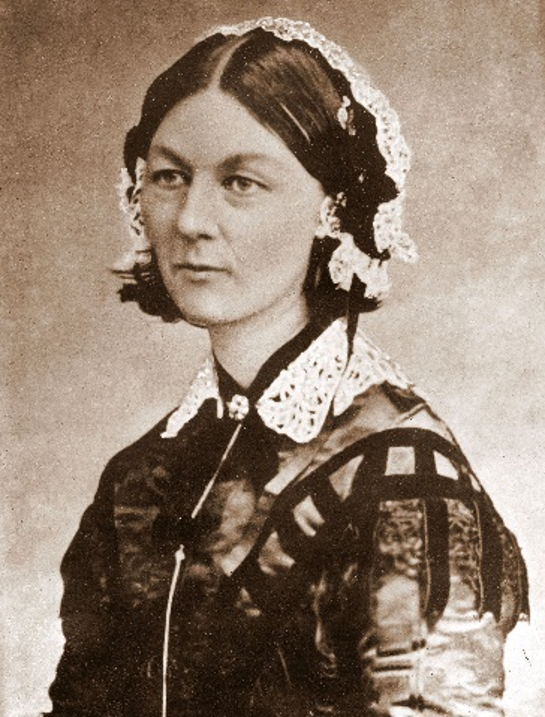
\includegraphics[keepaspectratio]{img/4-visualizacao-de-dados-tabulares/4-1-florence_nightingale.png}}

}

\end{figure}%

O que Nightingale encontrou em Scutari a levou a organizar um registro
meticuloso das causas de morte entre os soldados britânicos. Os números
mostravam que a maior parte das mortes não vinha dos combates, e sim de
doenças contraídas dentro do próprio hospital, como cólera, febre
tifoide e disenteria, favorecidas pela ausência de cuidados sanitários,
conforme se pode observar na Figura~\ref{fig-rose-diagram}. Nos
primeiros sete meses da campanha, a mortalidade por doença correspondia
sozinha a uma taxa anual de 60\%, superior à da Grande Peste de Londres
de 1665 (Friendly \& Andrews, 2021).

De volta à Inglaterra em julho de 1856, ela passou a pressionar o
governo britânico por reformas nos hospitais militares. Apresentou
relatórios extensos, cheios de tabelas e de propostas concretas, e pouco
aconteceu. Foi então que recorreu a um recurso que acabaria por mudar a
história da comunicação de dados.

\begin{figure}[H]

\caption{\label{fig-rose-diagram}Diagrama da Rosa, apresentando as
causas de mortalidade no exército britânico no Oriente, publicado por
Florence Nightingale em 1859. A rosa da direita cobre o período de abril
de 1854 a março de 1855, e a da esquerda cobre de abril de 1855 a março
de 1856. Fonte: Nightingale (1859).}

\centering{

\pandocbounded{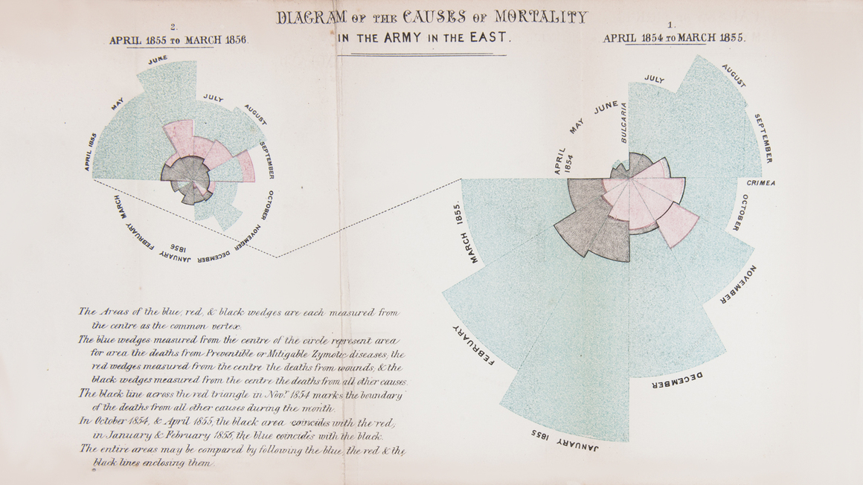
\includegraphics[keepaspectratio]{img/4-visualizacao-de-dados-tabulares/4-2-rose_diagram.png}}

}

\end{figure}%

O diagrama representa cada mês do conflito como uma fatia de ângulo
igual, cuja extensão a partir do centro corresponde à mortalidade
daquele mês. As áreas azuis indicam mortes por doenças evitáveis, as
vermelhas indicam mortes por ferimentos de combate e as cinzas indicam
as demais causas, como acidentes e queimaduras. A separação em duas
rosas é proposital, pois a Comissão Sanitária encarregada de investigar
as condições dos hospitais chegou à região em março de 1855, exatamente
na fronteira entre os dois períodos representados (Friendly \& Andrews,
2021).

A comparação entre as duas rosas dispensa qualquer cálculo. O azul
domina a figura inteira e encolhe visivelmente no segundo período. Em
uma única imagem ficava demonstrado que os soldados morriam sobretudo de
causas evitáveis e que as medidas sanitárias funcionavam. O argumento
venceu onde os relatórios haviam falhado, e as reformas sanitárias foram
adotadas nos hospitais militares britânicos. A estratégia está resumida
em uma frase tradicionalmente atribuída a ela:

``O diagrama deve afetar através dos olhos o que não conseguimos
transmitir ao cérebro do público através dos seus ouvidos à prova de
palavras.''

Há no diagrama um detalhe que antecipa o assunto das próximas seções. Em
uma versão anterior, Nightingale representou a mortalidade pela
distância entre o centro e a ponta da fatia. Ela percebeu que o
resultado enganava, porque o olho lê a área da fatia e não o seu
comprimento, de modo que dobrar a taxa de mortalidade quadruplicava a
área percebida. Na versão final passou a usar a raiz quadrada da
distância, fazendo com que a área de cada fatia refletisse corretamente
o número de mortes (Friendly \& Andrews, 2021). Mais de um século antes
de a psicologia da percepção ser sistematicamente incorporada ao projeto
de gráficos, ela já havia identificado o problema e o corrigido.

\section{Como percebemos elementos visuais}\label{sec-percepcao}

Todo gráfico codifica dados usando um repertório limitado de
propriedades gráficas. Sistematizá-las ajuda a perceber que a escolha
entre um gráfico e outro é, no fundo, uma escolha entre esses elementos
(Munzner, 2015):

\begin{itemize}
\tightlist
\item
  \textbf{posição}, o local que o dado ocupa no espaço do gráfico;
\item
  \textbf{tamanho}, a extensão linear das formas;
\item
  \textbf{ângulo}, a rotação entre dois vetores;
\item
  \textbf{inclinação}, a orientação de um vetor no espaço;
\item
  \textbf{forma}, o símbolo usado para representar categorias;
\item
  \textbf{área}, a extensão em duas dimensões;
\item
  \textbf{volume}, a extensão em três dimensões;
\item
  \textbf{matiz}, o tom ou coloração propriamente dito;
\item
  \textbf{saturação}, a intensidade da matiz.
\end{itemize}

\begin{figure}[H]

\caption{\label{fig-elementos-visuais}Elementos visuais disponíveis para
codificar dados em um gráfico. Fonte: adaptado de Munzner (2015).}

\centering{

\pandocbounded{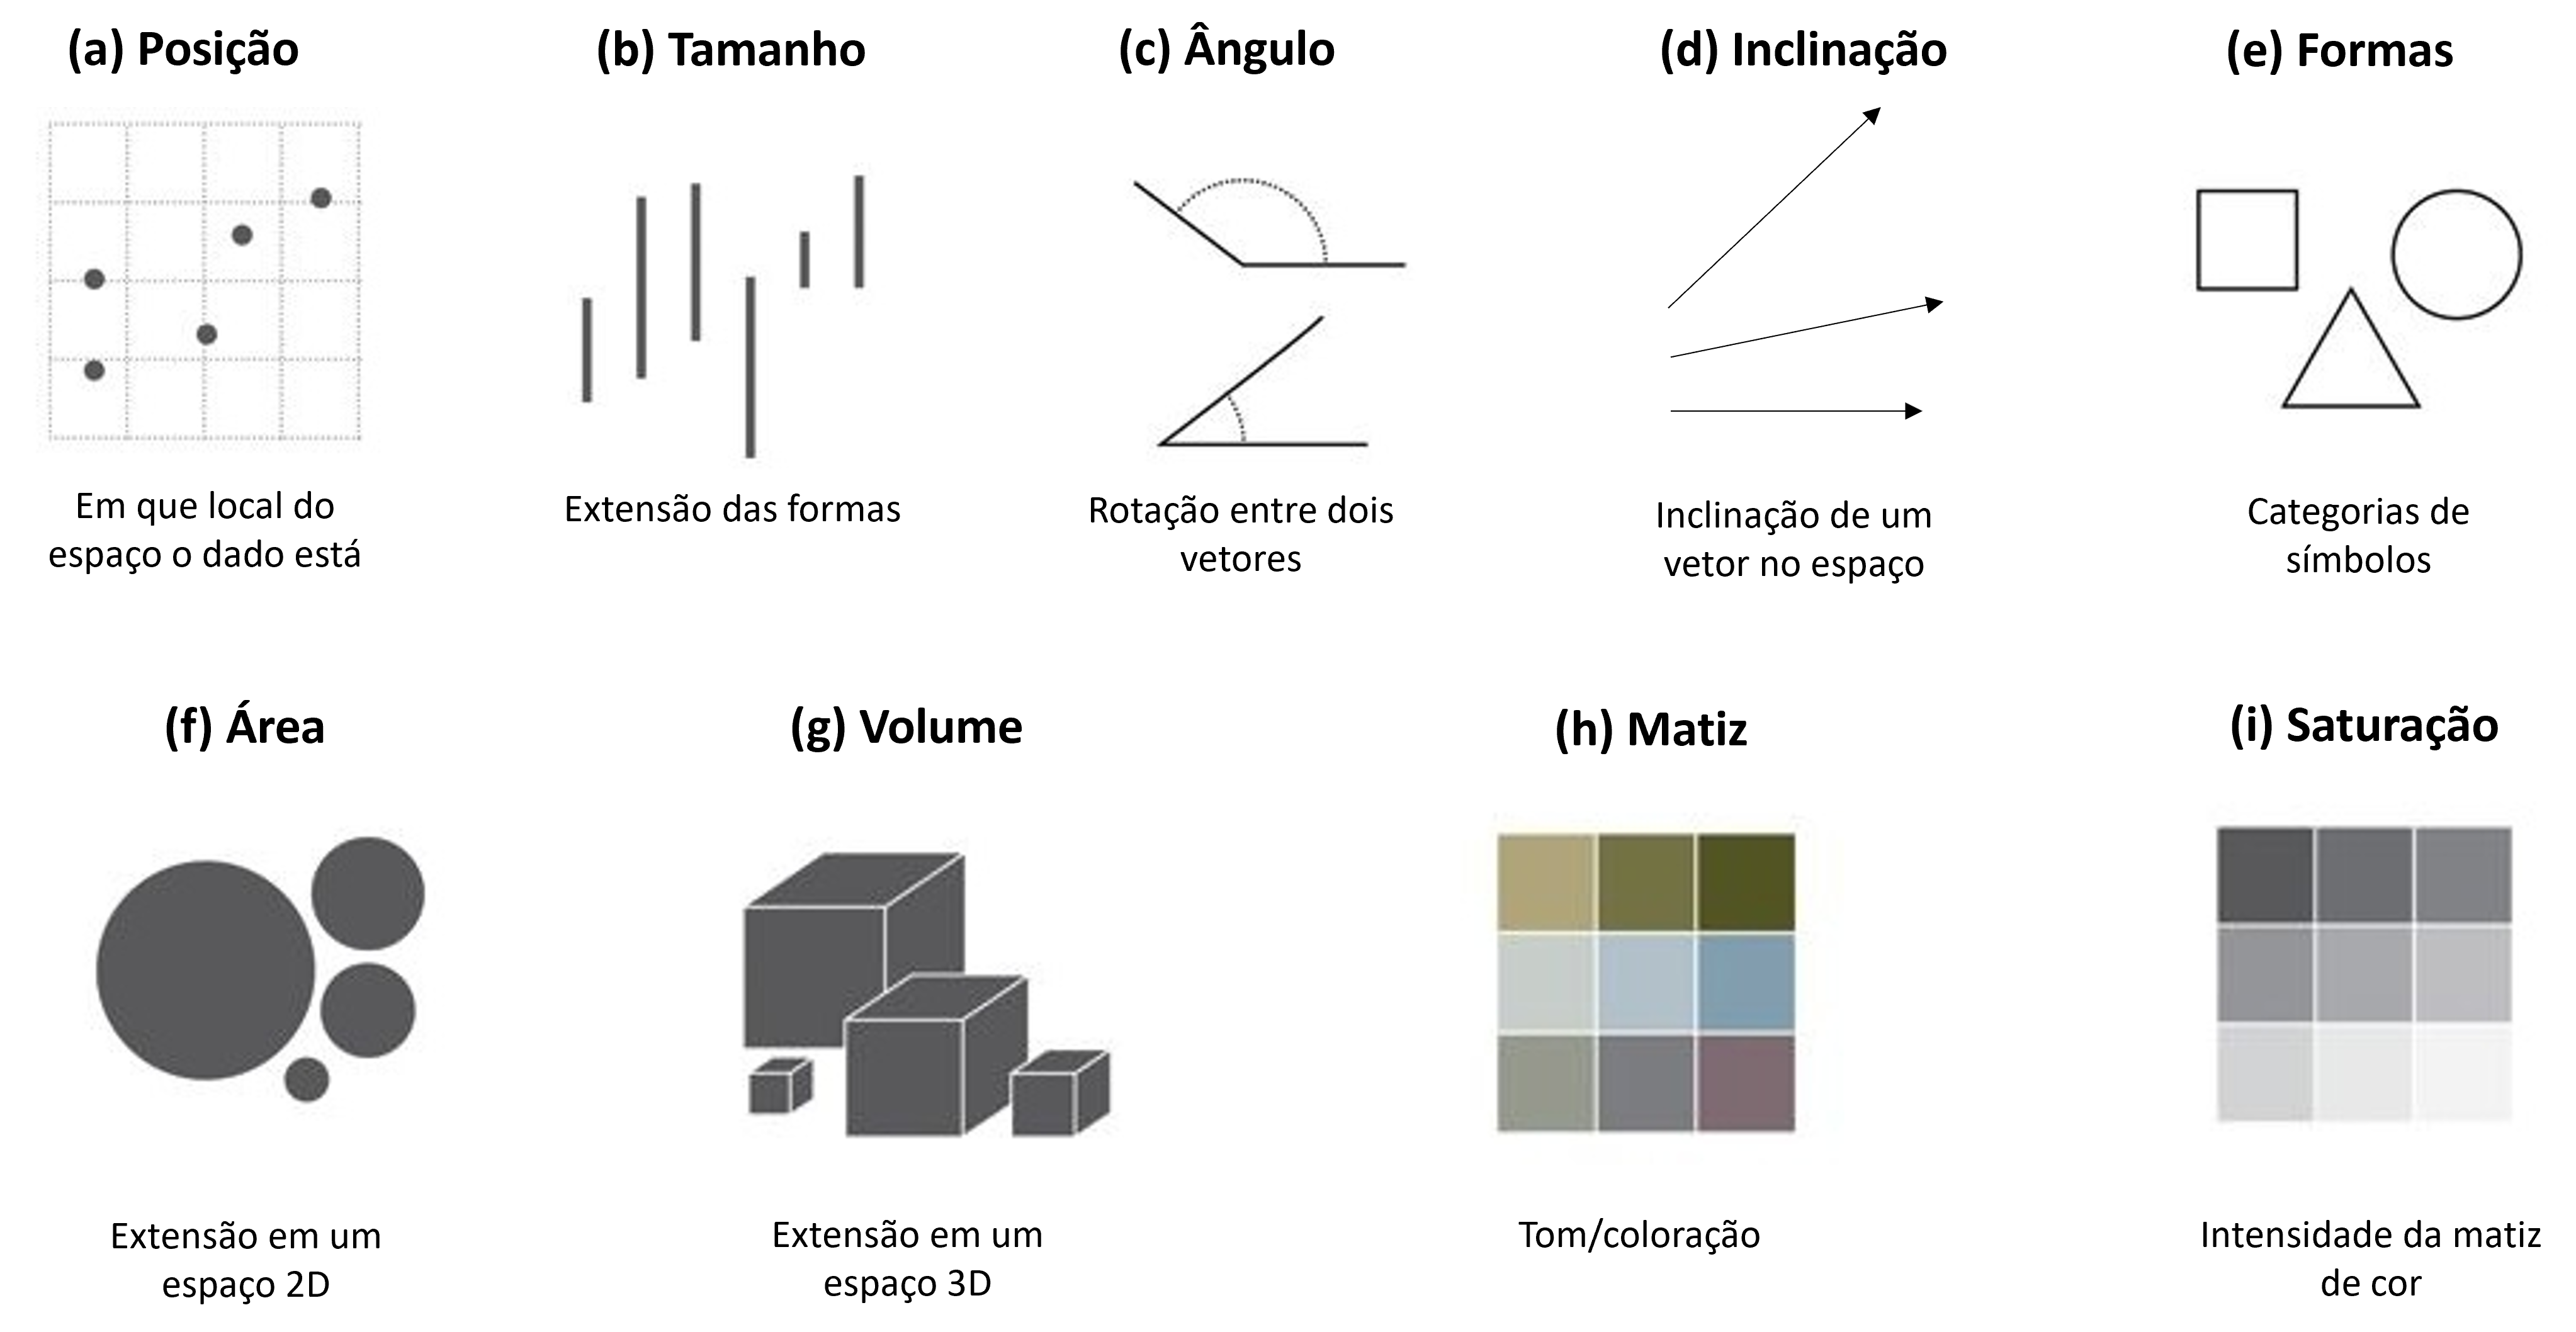
\includegraphics[keepaspectratio]{img/4-visualizacao-de-dados-tabulares/4-3-elementos_visuais.png}}

}

\end{figure}%

Os diferentes tipos de gráfico possuem como pecularidade exatamente um
ou mais destes elementos. Enquanto um gráfico de barras usa posição e
tamanho, um gráfico de setores\footnote{Coloquialmente conhecido como
  gráfico de \emph{pizza}} usa ângulo e área. Já um gráfico de dispersão
com pontos coloridos usa posição, matiz e eventualmente área. A pergunta
que importa é quão eficiente cada um desses elementos é no processo de
assimilação das informações que se pretende transmitir.

A resposta a essa pergunta pode ser dada a partir de um simples
exercício visual. A Figura~\ref{fig-tres-codificacoes} mostra um mesmo
conjunto de cinco valores codificado de três maneiras, por intensidade
de cor, por área de círculo e por altura de barra. Antes de prosseguir
na leitura, vale a pena parar e tentar responder, para cada um dos três
painéis, quantas vezes o valor de D é maior que o de E.

\begin{figure}[H]

\caption{\label{fig-tres-codificacoes}Um mesmo conjunto de valores
codificado por intensidade de cor (a), por área de círculo (b) e por
altura de barra (c). Elaboração própria, com base na demonstração de
Munzner (2015).}

\centering{

\pandocbounded{
\includegraphics[keepaspectratio]{4-visualizacao-de-dados-tabulares_files/figure-pdf/fig-tres-codificacoes-1.pdf}}

}

\end{figure}%

Os valores são exatamente os mesmos nos três painéis, e D vale cinco
vezes E. Com intensidade de cor conseguimos no máximo ordenar
grosseiramente as categorias, sem nenhuma noção da razão entre elas. Com
área acertamos a ordem e subestimamos a diferença, porque o olho
comprime a percepção de área. Com altura de barra a razão de cinco para
um é lida com boa precisão. A comparação, portanto, é progressivamente
mais fácil da primeira para a terceira representação.

Esse resultado não é uma impressão subjetiva. Estudos experimentais
foram realizados em ocasiões diferentes e chegaram à mesma ordenação
(Cleveland \& McGill, 1985; Heer \& Bostock, 2010)\footnote{Cleveland \&
  McGill (1985) conduziram experimentos controlados medindo o erro
  cometido por participantes ao estimar quantidades codificadas por
  diferentes elementos visuais, e obtiveram uma ordenação estável entre
  eles. Vinte e cinco anos depois, Heer \& Bostock (2010) repetiram
  esses experimentos recorrendo a uma plataforma de trabalho
  colaborativo pela internet, o que lhes permitiu recrutar um conjunto
  de participantes muito maior e mais heterogêneo do que era viável em
  laboratório. Os resultados anteriores foram reproduzidos, e o estudo
  ainda os estendeu a codificações não contempladas originalmente, como
  a área de retângulos.}. A hierarquia resultante desses estudos
(Figura~\ref{fig-hierarquia-percepcao}) coloca no topo a posição em
escala comum e alinhada, seguida da posição em escala comum mas
desalinhada, da extensão, do ângulo, da inclinação, da área, do volume,
da intensidade de cor e, por último, da matiz. Consequentemente, quando
o objetivo é comparar quantidades com precisão, convém usar elementos do
topo da hierarquia.

\begin{figure}[H]

\caption{\label{fig-hierarquia-percepcao}Hierarquia de percepção dos
elementos visuais. Os elementos no topo permitem comparações
quantitativas mais precisas, e os da base permitem apenas comparações
genéricas. Fonte: adaptado de Cleveland \& McGill (1985) e Munzner
(2015).}

\centering{

\pandocbounded{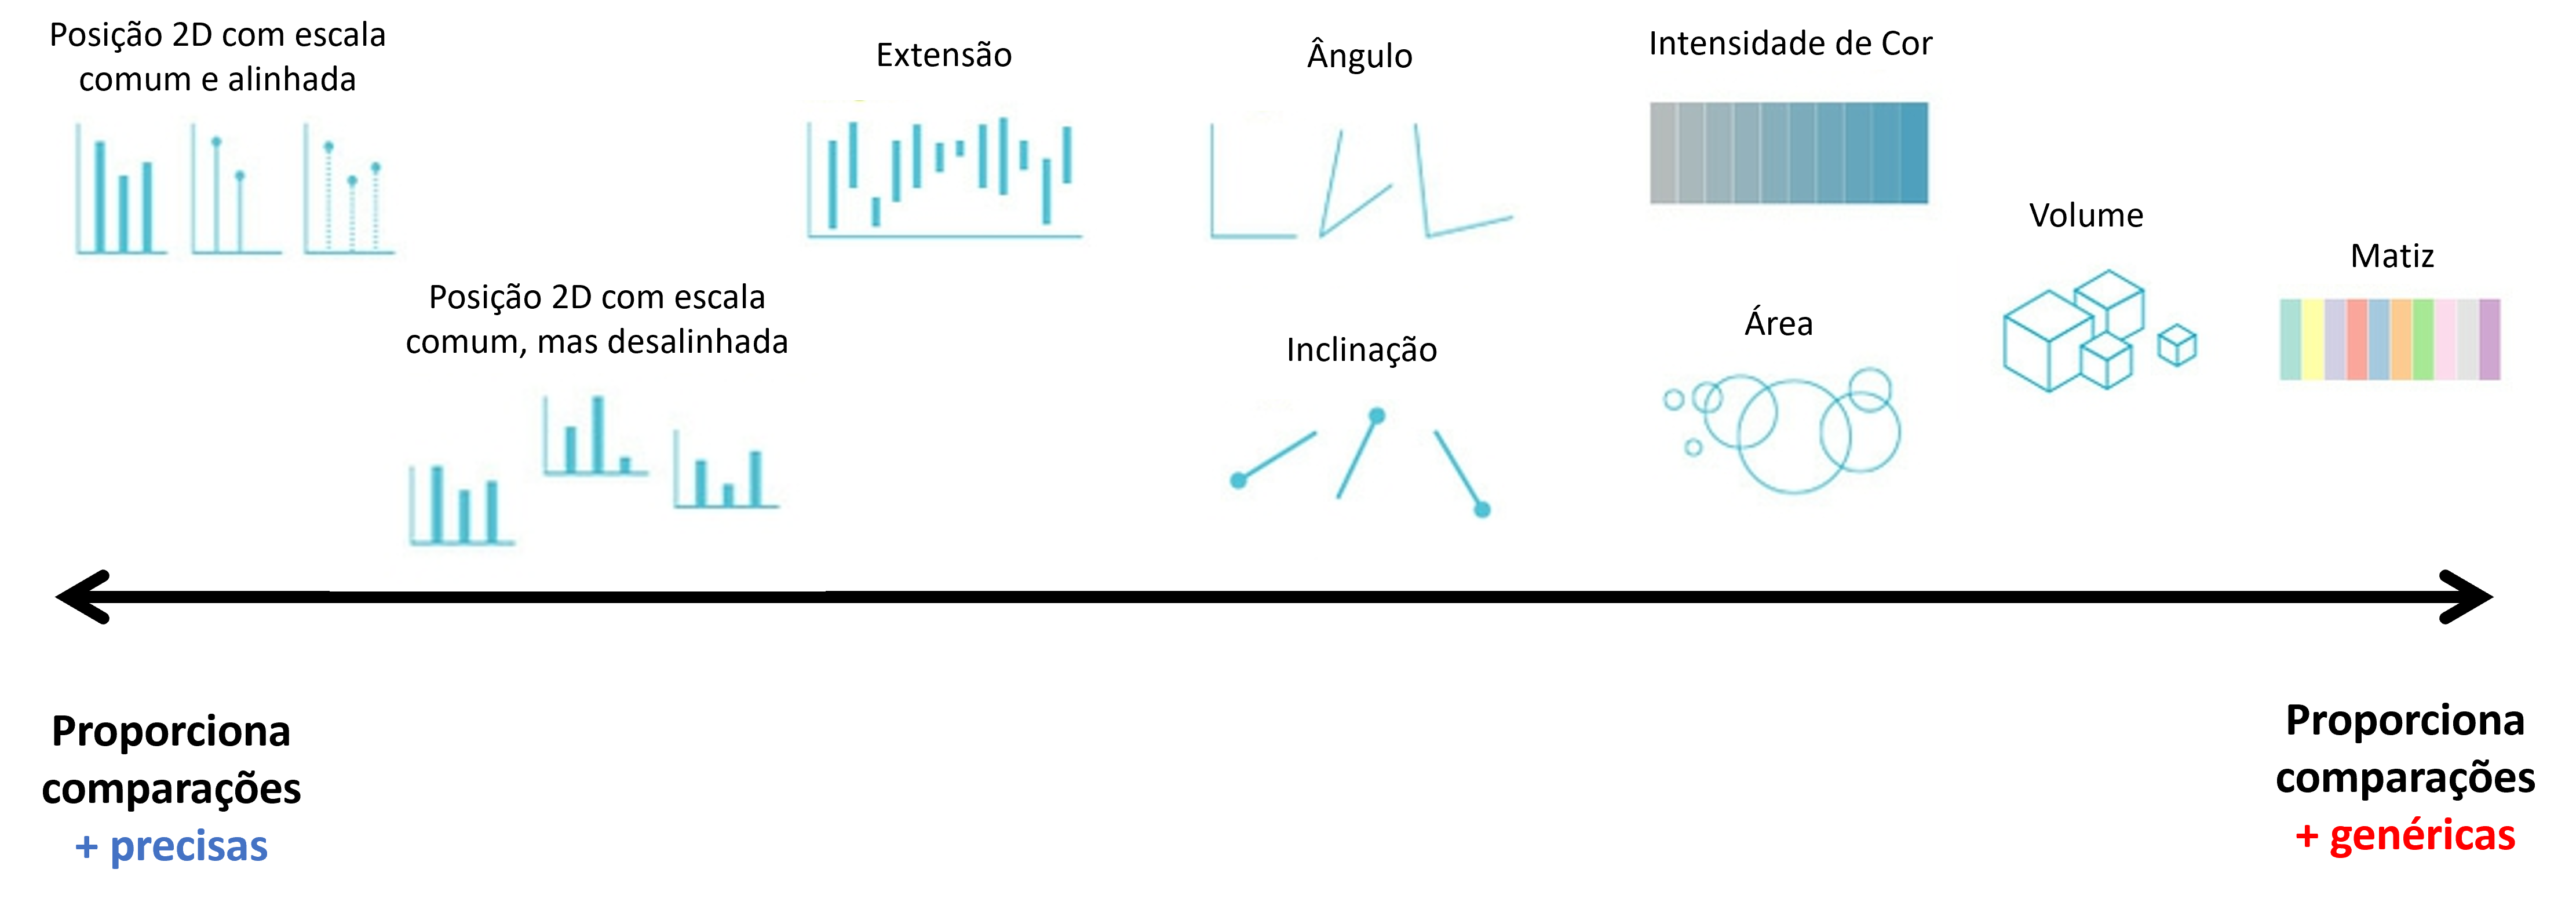
\includegraphics[keepaspectratio]{img/4-visualizacao-de-dados-tabulares/4-5-hierarquia_elem_visuais.png}}

}

\end{figure}%

Isso não significa que os elementos da base sejam inúteis, e sim que
eles servem a outro propósito ou apoiam a intuição de forma secundária.
Um exemplo do primeiro caso é a matiz, bastante contraindicada para
representar magnitude, porém excelente para distinguir categorias,
porque o cérebro humano reconhece diferenças de tom com facilidade sem
tentar quantificá-las.

O segundo caso aparece sempre que a leitura precisa fica a cargo de
outro elemento e a codificação de baixa hierarquia apenas orienta o
olhar. É o que veremos adiante neste capítulo no gráfico de dispersão em
que uma terceira variável é representada pela intensidade de cor ou pelo
tamanho dos pontos. A posição nos eixos sustenta a leitura precisa das
duas primeiras variáveis, enquanto a cor ou área do ponto apenas indica
se a terceira cresce ou diminui ao longo dos valores de \(x\) e \(y\),
sem permitir comparação numérica direta entre observações.

\section{A gramática dos gráficos}\label{a-gramuxe1tica-dos-gruxe1ficos}

\subsection{Por que uma gramática}\label{por-que-uma-gramuxe1tica}

Até aqui discutimos gráficos como objetos prontos, escolhidos de um
catálogo. Quem aprende visualização dessa maneira acaba com uma lista
mental de tipos de gráficos (barras, setores, dispersão, histograma,
\emph{boxplot}, \ldots) e com a tarefa de escolher um deles a cada
análise. O problema dessa abordagem é que a lista é bastante extensa,
não explica por que um tipo funciona melhor que outro e não ajuda em
nada quando a situação não se encaixa em nenhum item do catálogo.

\begin{figure}[H]

\caption{\label{fig-grammar_of_graphics}Capa da segunda edição de
\emph{The Grammar of Graphics}, de Leland Wilkinson.}

\centering{

\pandocbounded{
\includegraphics[keepaspectratio]{img/4-visualizacao-de-dados-tabulares/4-6-grammar_of_graphics.png}}

}

\end{figure}%

Em 1999, Leland Wilkinson propôs uma inversão dessa perspectiva em um
trabalho que se tornou uma das referências teóricas mais influente da
área, denominado a \textbf{Gramática dos Gráficos}\footnote{do inglês,
  \emph{Grammar of Graphics}} (Wilkinson, 2005). O argumento central é
que um gráfico não existe por si próprio, da mesma forma que uma frase
não existe independentemente das palavras que a compõem. Sabemos que uma
língua é muito mais que um repertório de frases prontas a serem
memorizadas. Ela é um vocabulário extenso somado a regras de combinação,
e dessa interação nasce a possibilidade de formular frases que ninguém
jamais pronunciou. Wilkinson percebeu que gráficos funcionam do mesmo
modo, ou seja, que existe um conjunto pequeno de componentes cujas
combinações geram praticamente qualquer representação visual de dados,
inclusive as que ainda não foram inventadas.

A consequência mais imediata dessa mudança de olhar é que a taxonomia
dos tipos de gráfico se dissolve. O que parecem duas modalidades
distintas costuma ser a mesma construção com uma única camada trocada. O
caso mais eloquente é o par formado pelo gráfico de barras empilhadas e
pelo gráfico de setores, caracterizando duas representações diferentes
para a mesma informação.

\begin{figure}[H]

\caption{\label{fig-cartesiano-polar}Uma mesma barra empilhada
representada em coordenadas cartesianas (a) e em coordenadas polares
(b). A segunda é o que costumamos chamar de gráfico de setores.}

\centering{

\pandocbounded{
\includegraphics[keepaspectratio]{4-visualizacao-de-dados-tabulares_files/figure-pdf/fig-cartesiano-polar-1.pdf}}

}

\end{figure}%

\subsection{As camadas de um gráfico}\label{as-camadas-de-um-gruxe1fico}

A composição proposta pela Gramática dos Gráficos é \textbf{modular} e
organizada em camadas sobrepostas, o que permite construir praticamente
qualquer modalidade de gráfico a partir de um conjunto pequeno de
decisões.

\begin{figure}[H]

\caption{\label{fig-camadas-gg}Composição de um gráfico em camadas
sobrepostas, conforme a gramática dos gráficos.}

\centering{

\pandocbounded{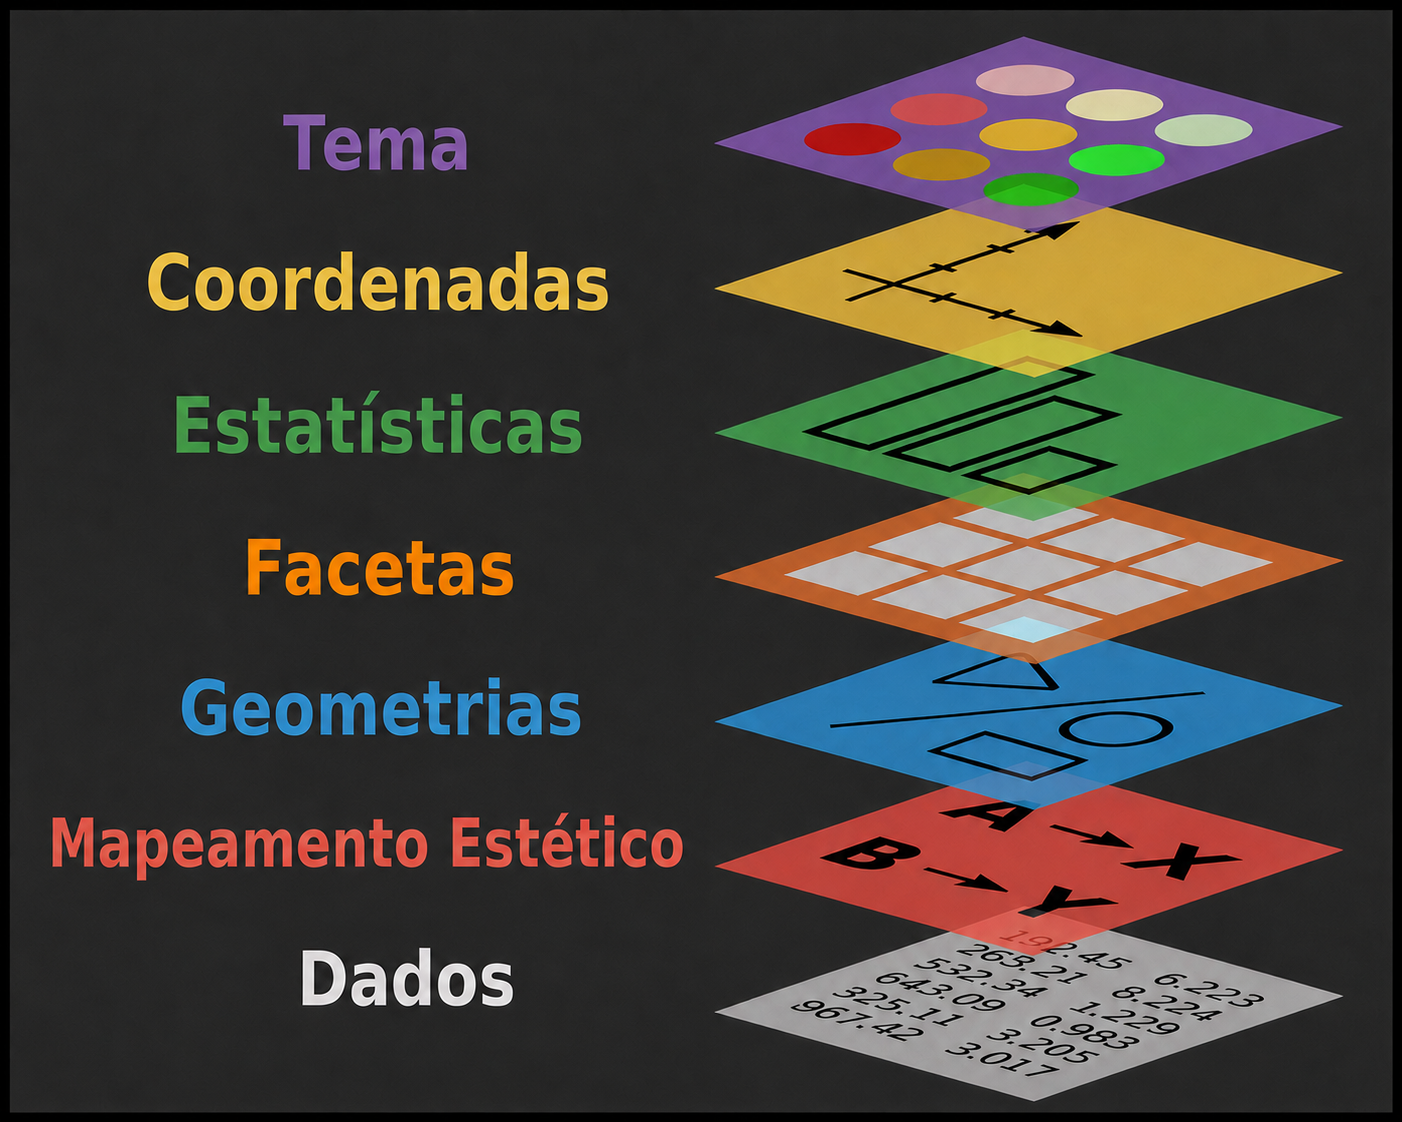
\includegraphics[keepaspectratio]{img/4-visualizacao-de-dados-tabulares/4-8-grammar_of_graphics_layers.png}}

}

\end{figure}%

As camadas se dividem em dois grupos. O primeiro reúne os elementos
fundamentais, sem os quais não há gráfico algum:

\begin{itemize}
\item
  Os \textbf{dados} (\emph{data}) são a tabela que fornece os valores a
  representar. Na gramática, ela é a primeira camada, pois determina o
  que é possível representar. Uma tabela em que cada linha é uma
  observação e cada coluna é uma variável, formato que vimos no capítulo
  anterior, é exatamente o que a gramática pressupõe.
\item
  O \textbf{mapeamento estético} (\emph{aesthetics} ou \emph{aesthetic
  mapping}) é a conexão entre cada variável da tabela e a propriedade
  gráfica que a representará. É aqui que a discussão da seção anterior
  entra na prática, porque mapear uma variável ao eixo \(x\), à cor ou
  ao tamanho dos pontos são decisões com consequências perceptivas muito
  diferentes. O mapeamento é a camada que traduz números em elementos
  visuais.
\item
  A \textbf{geometria} (\emph{geometry}) é a forma visual concreta que
  traduz esse mapeamento, como pontos, barras, linhas ou caixas. Um
  mesmo mapeamento admite geometrias diferentes. Duas variáveis
  numéricas mapeadas aos eixos \(x\) e \(y\) podem virar uma nuvem de
  pontos ou uma linha, e a escolha entre elas depende de a relação entre
  as observações ser de comparação ou de continuidade.
\end{itemize}

O segundo grupo reúne os elementos complementares, que refinam o
resultado sem alterar sua estrutura básica:

\begin{itemize}
\item
  As \textbf{estatísticas} (\emph{statistics}) inserem no gráfico
  quantidades calculadas a partir dos dados em vez dos valores
  originais. Essa camada costuma passar despercebida porque quase sempre
  age de forma silenciosa. Um histograma, por exemplo, agrupa os valores
  em classes e desenha a \emph{contagem} de cada classe. Um gráfico de
  barras construído a partir de uma variável categórica também
  \emph{conta} observações antes de desenhar, e um boxplot calcula
  \emph{quartis} e \emph{limites} antes de traçar a caixa.
\item
  As \textbf{escalas} (\emph{scales}) definem como os valores das
  variáveis se convertem em valores concretos da propriedade gráfica, ou
  seja, quais números correspondem a quais posições no eixo, a quais
  cores e a quais tamanhos. Toda variável mapeada recebe automaticamente
  uma escala, e ajustá-la é o que permite trocar uma paleta de cores,
  inverter um eixo ou garantir que a área dos círculos seja proporcional
  ao valor representado.
\item
  O \textbf{sistema de coordenadas} (\emph{coordinates}) organiza o
  espaço em que as geometrias são desenhadas, podendo ser cartesiano ou
  polar, por exemplo.
\item
  As \textbf{facetas} (\emph{facets}) subdividem o gráfico em painéis
  segundo os níveis de uma ou duas variáveis categóricas, repetindo a
  mesma construção para cada subconjunto dos dados. É o recurso que
  permite comparar grupos sem sobrecarregar um único painel.
\item
  O \textbf{tema} (\emph{theme}) reúne os ajustes estéticos que não
  codificam dado algum, como cor de fundo, presença de grades, tamanho
  de fonte e posição da legenda.
\end{itemize}

Convém guardar essa divisão, porque ela organiza tudo o que faremos
daqui em diante. Diante de qualquer gráfico deste capítulo, vale o
exercício de identificar qual variável está em qual mapeamento, qual
geometria foi escolhida e quais camadas complementares foram acionadas.

\subsection{O ggplot2}\label{o-ggplot2}

A Gramática dos Gráficos orienta o desenvolvimento das principais
ferramentas de visualização em uso hoje, entre elas o Tableau, o Plotly
e bibliotecas de Python como \texttt{bokeh}, \texttt{altair},
\texttt{seaborn} e \texttt{plotnine}. Sua implementação mais completa,
porém, é o pacote \texttt{ggplot2} do R, onde o duplo \emph{g} inicial
vem justamente da sigla em inglês \emph{G}rammar of \emph{G}raphics.

O \texttt{ggplot2} foi desenvolvido por Hadley Wickham, que traduziu a
proposta de Wilkinson para código. Ao implementá-la, inclusive, ele a
reformulou naquilo que chamou de \textbf{gramática em camadas} (Wickham,
2010). Duas contribuições dessa reformulação explicam por que o pacote é
tão econômico de usar.

A primeira é a organização em camadas propriamente dita, que agrupa
dados, mapeamento, geometria e estatística em unidades sobrepostas. É
isso que torna possível somar elementos a um gráfico com o operador
\texttt{+}, escrevendo a construção na mesma ordem em que a pensamos. A
segunda é a \textbf{hierarquia de valores-padrão}. Todo gráfico precisa
das sete camadas para existir, e exigir que todas fossem declaradas a
cada vez tornaria o código muito comprido. O \texttt{ggplot2} deduz o
que não foi informado. Ao pedir um histograma, o pacote sabe que a
estatística é o agrupamento em classes, que o sistema de coordenadas é o
cartesiano, que a escala do eixo \(x\) é contínua e que o tema é o
padrão. Nada disso precisa ser escrito, e tudo isso pode ser sobrescrito
quando necessário. Por isso duas linhas de código produzem um gráfico
completo, e por isso mesmo vale insistir que as camadas continuam todas
lá, ainda que invisíveis no código.

Uma consequência prática dessa arquitetura é que o \texttt{ggplot2} não
tem uma função por tipo de gráfico, ou seja, não existe uma função
\texttt{hist()} e outra \texttt{barplot()} para se produzir os gráficos
isoladamente como no R base. Em vez disso, existem funções para cada
camada, e o tipo de gráfico emerge da combinação escolhida, como a
Tabela~\ref{tbl-camadas} resume.

\begin{longtable}[]{@{}
  >{\raggedright\arraybackslash}p{(\linewidth - 4\tabcolsep) * \real{0.3333}}
  >{\raggedright\arraybackslash}p{(\linewidth - 4\tabcolsep) * \real{0.3333}}
  >{\raggedright\arraybackslash}p{(\linewidth - 4\tabcolsep) * \real{0.3333}}@{}}
\caption{Correspondência entre as camadas da gramática dos gráficos e as
funções do \protect\texttt{ggplot2}.}\label{tbl-camadas}\tabularnewline
\toprule\noalign{}
\begin{minipage}[b]{\linewidth}\raggedright
Camada
\end{minipage} & \begin{minipage}[b]{\linewidth}\raggedright
Papel
\end{minipage} & \begin{minipage}[b]{\linewidth}\raggedright
Funções no \texttt{ggplot2}
\end{minipage} \\
\midrule\noalign{}
\endfirsthead
\toprule\noalign{}
\begin{minipage}[b]{\linewidth}\raggedright
Camada
\end{minipage} & \begin{minipage}[b]{\linewidth}\raggedright
Papel
\end{minipage} & \begin{minipage}[b]{\linewidth}\raggedright
Funções no \texttt{ggplot2}
\end{minipage} \\
\midrule\noalign{}
\endhead
\bottomrule\noalign{}
\endlastfoot
Dados & Tabela com os valores a representar &
\texttt{ggplot(data\ =\ ...)} \\
Mapeamento estético & Liga variáveis a propriedades gráficas &
\texttt{aes()} \\
Geometria & Forma visual que representa os dados &
\texttt{geom\_point()}, \texttt{geom\_col()},
\texttt{geom\_boxplot()} \\
Estatística & Transforma os dados antes de desenhá-los &
\texttt{stat\_*()} e o argumento \texttt{stat} das geometrias \\
Escalas & Converte valores em posições, cores e tamanhos &
\texttt{scale\_x\_continuous()}, \texttt{scale\_fill\_manual()} \\
Coordenadas & Organiza o espaço do gráfico &
\texttt{coord\_cartesian()}, \texttt{coord\_polar()},
\texttt{coord\_flip()} \\
Facetas & Subdivide o gráfico em painéis & \texttt{facet\_grid()},
\texttt{facet\_wrap()} \\
Tema & Ajustes estéticos que não codificam dados & \texttt{theme\_bw()},
\texttt{theme\_minimal()}, \texttt{theme()} \\
\end{longtable}

Essa tabela é a chave de leitura de todo o restante do capítulo. Cada
gráfico que produzirmos daqui em diante será uma escolha explícita de
algumas dessas linhas, com as demais assumindo seus valores-padrão. Para
quem quiser aprofundar o funcionamento do pacote camada por camada, a
referência é o livro do próprio autor (Wickham, 2016), disponível
gratuitamente em \href{https://ggplot2-book.org/}{ggplot2-book.org}.

O \texttt{ggplot2} faz parte do \texttt{tidyverse}, de modo que carregar
a coleção completa já o disponibiliza:

\begin{Shaded}
\begin{Highlighting}[]
\FunctionTok{library}\NormalTok{(tidyverse)}
\end{Highlighting}
\end{Shaded}

\section{O primeiro gráfico}\label{o-primeiro-gruxe1fico}

Trabalharemos com a base \texttt{escolha\_modal}, a mesma dos capítulos
anteriores. Lembre-se de fazer o download pelo link abaixo, salvando o
arquivo em uma pasta onde você irá criar o projeto no RStudio junto com
o script no qual executará o código para a criação dos gráficos:

\begin{itemize}
\tightlist
\item
  \href{https://github.com/pedreirajr/rcensolivro/releases/download/dados/escolha_modal.csv}{\texttt{escolha\_modal.csv}}
\end{itemize}

O código abaixo repete o encadeamento construído no capítulo anterior,
lendo o arquivo, convertendo as variáveis categóricas para
\emph{factor}, passando o tempo de viagem de minutos para horas e
criando a velocidade média da viagem:

\begin{Shaded}
\begin{Highlighting}[]
\NormalTok{em }\OtherTok{\textless{}{-}} \FunctionTok{read\_csv}\NormalTok{(}\StringTok{"escolha\_modal.csv"}\NormalTok{, }\AttributeTok{locale =} \FunctionTok{locale}\NormalTok{(}\AttributeTok{encoding =} \StringTok{"Latin1"}\NormalTok{)) }\SpecialCharTok{|\textgreater{}}
  \FunctionTok{mutate}\NormalTok{(}
    \AttributeTok{sexo             =} \FunctionTok{factor}\NormalTok{(sexo),}
    \AttributeTok{posse\_auto       =} \FunctionTok{factor}\NormalTok{(posse\_auto),}
    \AttributeTok{modo\_viagem      =} \FunctionTok{factor}\NormalTok{(modo\_viagem),}
    \AttributeTok{tempo\_viagem     =}\NormalTok{ tempo\_viagem }\SpecialCharTok{/} \DecValTok{60}\NormalTok{,}
    \AttributeTok{vel\_media\_viagem =}\NormalTok{ dist\_viagem }\SpecialCharTok{/}\NormalTok{ tempo\_viagem}
\NormalTok{  )}
\end{Highlighting}
\end{Shaded}

Vale conferir rapidamente a estrutura resultante antes de seguir:

\begin{Shaded}
\begin{Highlighting}[]
\FunctionTok{glimpse}\NormalTok{(em)}
\end{Highlighting}
\end{Shaded}

\begin{verbatim}
Rows: 1,000
Columns: 8
$ sexo             <fct> F, F, F, F, M, M, F, F, M, M, M, F, M, M, M, F, M, M,~
$ idade            <dbl> 34, 43, 55, 45, 45, 36, 18, 31, 53, 40, 58, 19, 33, 3~
$ renda            <dbl> 3797, 3515, 4791, 2749, 2929, 2011, 1084, 2338, 7473,~
$ posse_auto       <fct> N, N, S, N, N, N, N, N, S, N, S, N, S, N, N, N, N, S,~
$ modo_viagem      <fct> Carro ou App, Carro ou App, TP, A pé, Carro ou App, T~
$ dist_viagem      <dbl> 14.3, 36.1, 26.9, 2.9, 20.6, 22.6, 29.6, 26.9, 18.3, ~
$ tempo_viagem     <dbl> 0.4500000, 0.9166667, 1.0666667, 0.4333333, 0.7333333~
$ vel_media_viagem <dbl> 31.777778, 39.381818, 25.218750, 6.692308, 28.090909,~
\end{verbatim}

A base tem 1.000 observações e sete variáveis originais, além da
velocidade média que acabamos de criar. Há três variáveis categóricas
(\texttt{sexo}, \texttt{posse\_auto} e \texttt{modo\_viagem}) e cinco
numéricas (\texttt{idade}, \texttt{renda}, \texttt{dist\_viagem},
\texttt{tempo\_viagem} e \texttt{vel\_media\_viagem}), combinação que
nos permitirá percorrer todos os casos deste capítulo.

A primeira função que trabalharemos do pacote é a \texttt{ggplot()}, que
recebe dois argumentos principais, que correspondem exatamente às duas
primeiras camadas da gramática. O argumento \texttt{data} recebe a
tabela, e o argumento \texttt{mapping} recebe a função \texttt{aes()},
dentro da qual declaramos a correspondência entre as variáveis
correspondem a as propriedades gráficas. Vejamos o que acontece ao
informar somente esses dois argumentos:

\begin{Shaded}
\begin{Highlighting}[]
\FunctionTok{ggplot}\NormalTok{(}\AttributeTok{data =}\NormalTok{ em, }\AttributeTok{mapping =} \FunctionTok{aes}\NormalTok{(}\AttributeTok{x =}\NormalTok{ renda))}
\end{Highlighting}
\end{Shaded}

\begin{figure}[H]

\caption{\label{fig-ggplot-vazio}Resultado de uma chamada a
\texttt{ggplot()} sem geometria. O sistema de eixos é construído, mas
nada é desenhado.}

\centering{

\pandocbounded{
\includegraphics[keepaspectratio]{4-visualizacao-de-dados-tabulares_files/figure-pdf/fig-ggplot-vazio-1.pdf}}

}

\end{figure}%

O R desenhou o painel e a escala do eixo \(x\) correspondente à variável
\texttt{renda}, sem ter desenhado nenhum elemento gráfico. Isso ocorre
porque falta a terceira camada fundamental, a geometria. As geometrias
são adicionadas com o operador \texttt{+} após \texttt{ggplot()},
conforme o exemplo da \texttt{geom\_histogram()} abaixo que desenha um
histograma para a variável renda:

\begin{Shaded}
\begin{Highlighting}[]
\FunctionTok{ggplot}\NormalTok{(}\AttributeTok{data =}\NormalTok{ em, }\AttributeTok{mapping =} \FunctionTok{aes}\NormalTok{(}\AttributeTok{x =}\NormalTok{ renda)) }\SpecialCharTok{+}
  \FunctionTok{geom\_histogram}\NormalTok{()}
\end{Highlighting}
\end{Shaded}

\begin{figure}[H]

\caption{\label{fig-ggplot-primeiro}Histograma da renda obtido com as
três camadas fundamentais da gramática.}

\centering{

\pandocbounded{
\includegraphics[keepaspectratio]{4-visualizacao-de-dados-tabulares_files/figure-pdf/fig-ggplot-primeiro-1.pdf}}

}

\end{figure}%

Com duas linhas de código tratamos de três das sete camadas da
gramática. Os nomes dos argumentos podem ser omitidos, já que
\texttt{data} e \texttt{mapping} são o primeiro e o segundo parâmetros
da função. É também comum encadear a base de dados inicialmente com o
pipe, o que se torna conveniente quando é preciso transformar os dados
antes de plotá-los. Verifique, no seu computador, como as três formas
abaixo produzem o mesmo resultado:

\begin{Shaded}
\begin{Highlighting}[]
\FunctionTok{ggplot}\NormalTok{(}\AttributeTok{data =}\NormalTok{ em, }\AttributeTok{mapping =} \FunctionTok{aes}\NormalTok{(}\AttributeTok{x =}\NormalTok{ renda)) }\SpecialCharTok{+}
  \FunctionTok{geom\_histogram}\NormalTok{()}

\FunctionTok{ggplot}\NormalTok{(em, }\FunctionTok{aes}\NormalTok{(}\AttributeTok{x =}\NormalTok{ renda)) }\SpecialCharTok{+}
  \FunctionTok{geom\_histogram}\NormalTok{()}

\NormalTok{em }\SpecialCharTok{|\textgreater{}}
  \FunctionTok{ggplot}\NormalTok{(}\FunctionTok{aes}\NormalTok{(}\AttributeTok{x =}\NormalTok{ renda)) }\SpecialCharTok{+}
  \FunctionTok{geom\_histogram}\NormalTok{()}
\end{Highlighting}
\end{Shaded}

\begin{tcolorbox}[enhanced jigsaw, arc=.35mm, bottomrule=.15mm, bottomtitle=1mm, breakable, colback=white, colbacktitle=quarto-callout-warning-color!10!white, colframe=quarto-callout-warning-color-frame, coltitle=black, left=2mm, leftrule=.75mm, opacityback=0, opacitybacktitle=0.6, rightrule=.15mm, title=\textcolor{quarto-callout-warning-color}{\faExclamationTriangle}\hspace{0.5em}{\texttt{+} e \texttt{\textbar{}\textgreater{}} não são intercambiáveis}, titlerule=0mm, toprule=.15mm, toptitle=1mm]

O operador \texttt{\textbar{}\textgreater{}} encadeia transformações de
dados, passando o resultado de uma função como primeiro argumento da
seguinte. O operador \texttt{+} empilha camadas de um gráfico já
iniciado por \texttt{ggplot()}. Trocar um pelo outro gera erro. Na
prática, o \texttt{\textbar{}\textgreater{}} aparece antes da chamada a
\texttt{ggplot()} e o \texttt{+} aparece depois dela.

\end{tcolorbox}

Para apresentarmos de forma mais sistematizada o desenvolvimento dos
tipos de gráfico mais fundamentais, subdiviremos o nosso fluxo de
trabalho nas três subseções a seguir:

\begin{itemize}
\item
  Visualização de \textbf{uma única variável}.
\item
  Visualização de \textbf{duas variáveis}.
\item
  Visualização de \textbf{três ou mais variáveis}.
\end{itemize}

\section{Visualizando uma única
variável}\label{visualizando-uma-uxfanica-variuxe1vel}

Com uma única variável, a escolha do gráfico depende essencialmente da
escala de mensuração desta variável (se numérica ou categórica),
conforme demonstrado na Figura~\ref{fig-unica-variavel}. Para variáveis
numéricas queremos enxergar a forma da distribuição, onde os valores se
concentram e quão dispersos eles são, e as ferramentas usuais são o
histograma e o boxplot. Para variáveis categóricas queremos contar
observações em cada nível, e a ferramenta usual é o gráfico de barras.

\begin{figure}[H]

\caption{\label{fig-unica-variavel}Principais tipos de visualização para
uma única variável}

\centering{

\pandocbounded{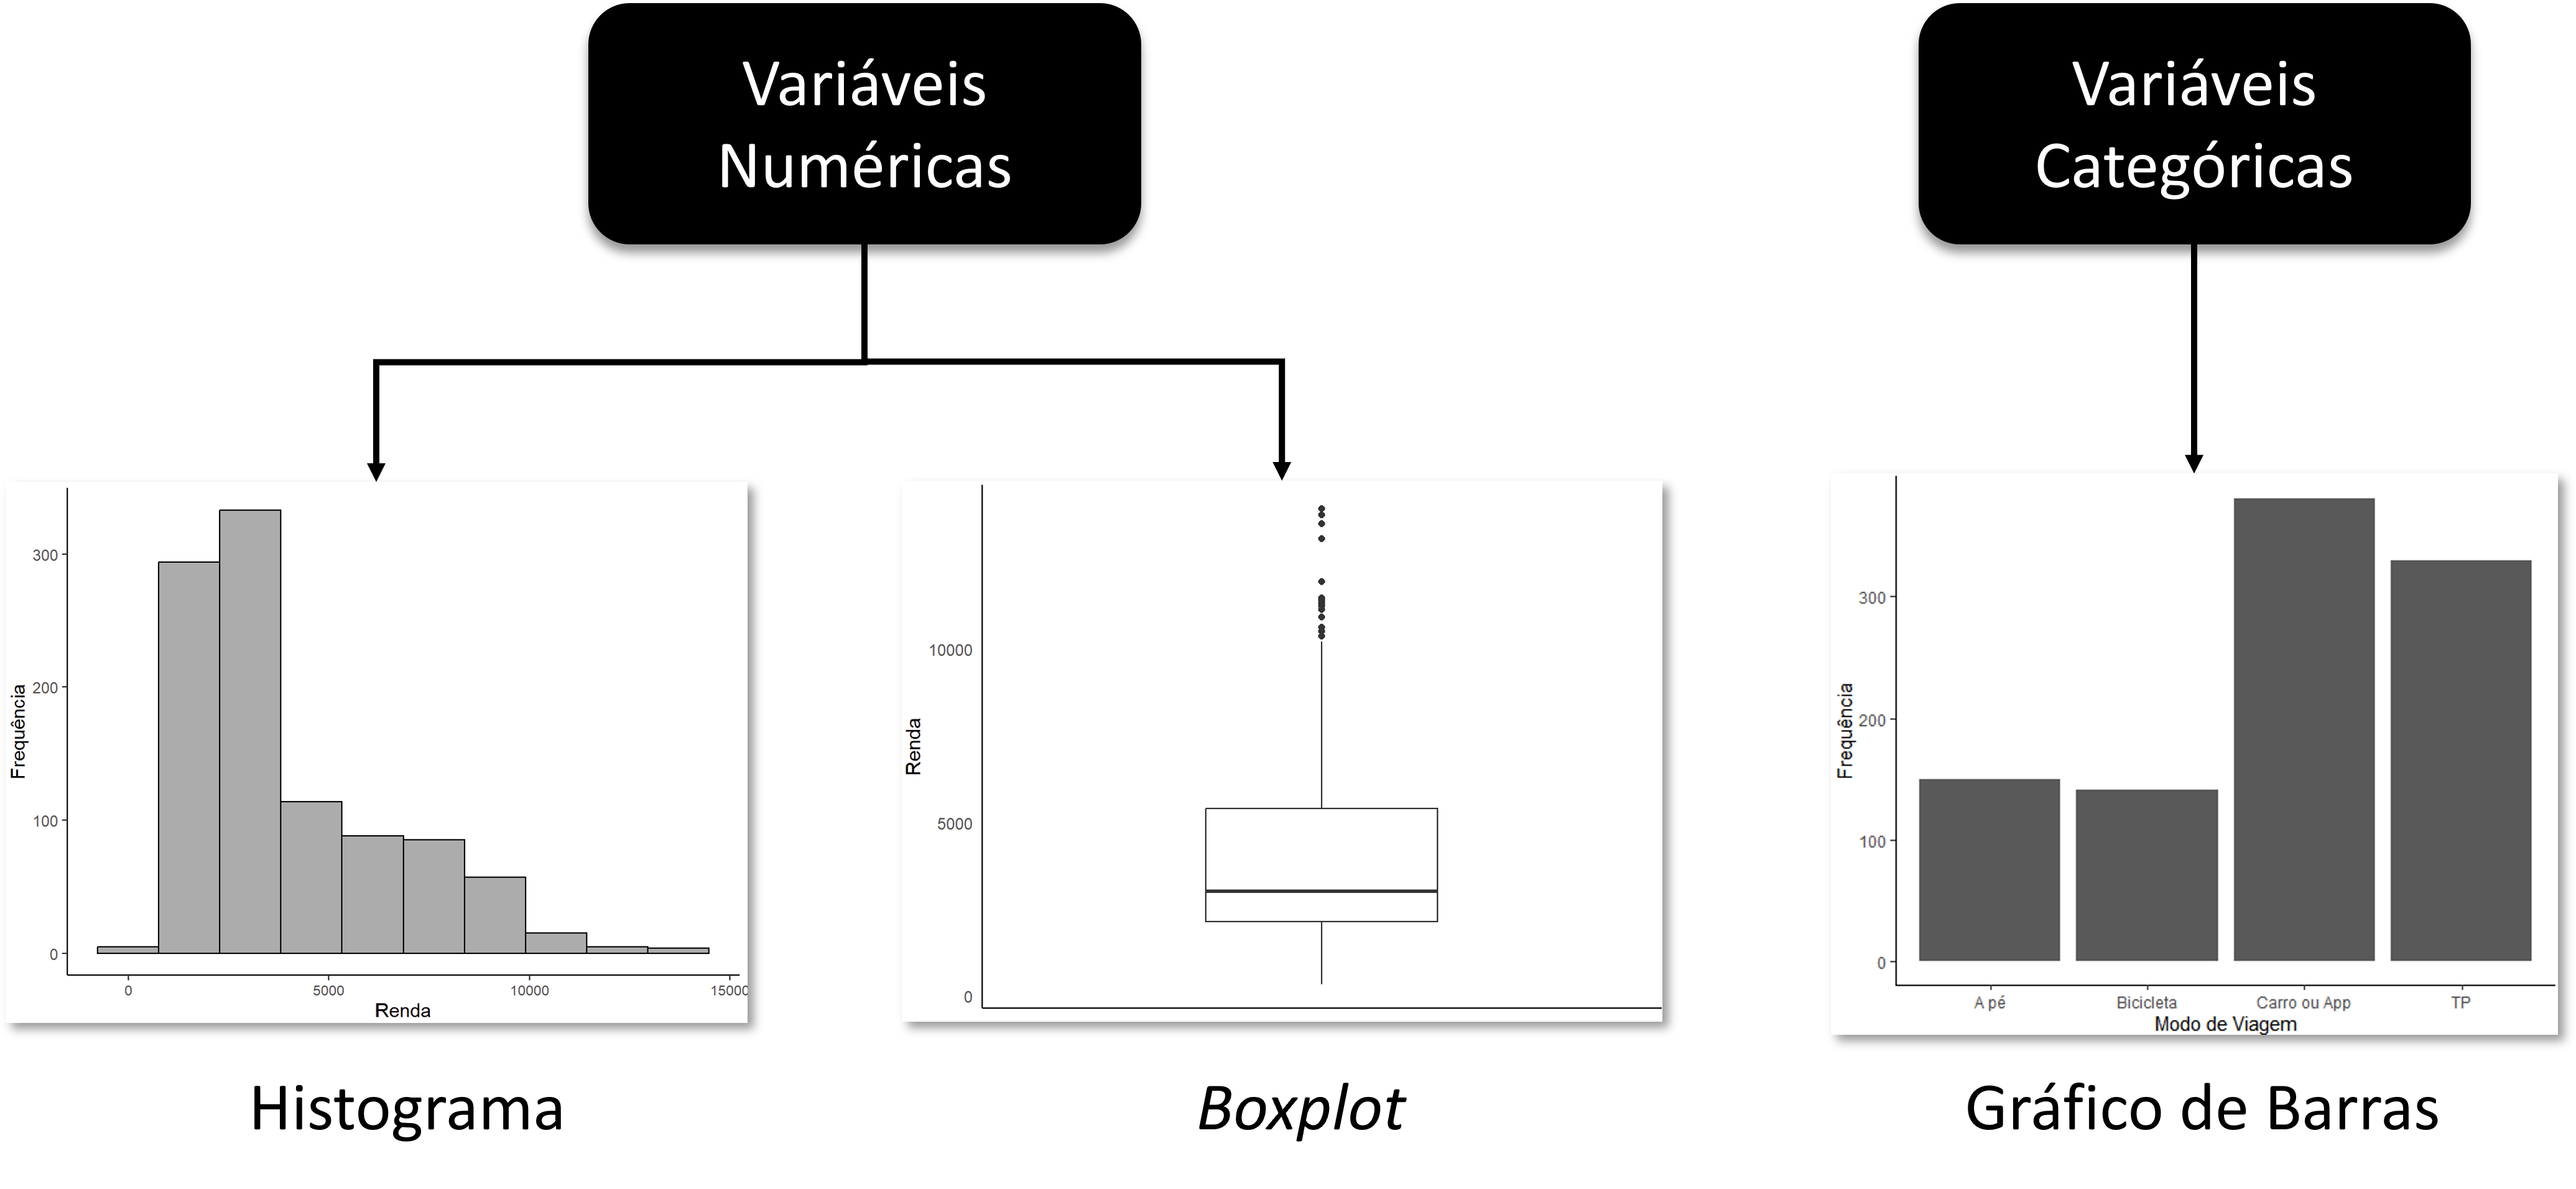
\includegraphics[keepaspectratio]{img/4-visualizacao-de-dados-tabulares/4-11-uma_unica_variavel.png}}

}

\end{figure}%

Apesar da leitura do gráfico de barras ser bem direta, existem aspectos
teóricos importantes a serem discutidos a respeito de histogramas e do
\emph{boxplot}, que serão discutidos de forma mais minuciosa nas
próximas seções.

\subsection{O histograma}\label{o-histograma}

O histograma divide o intervalo de valores da variável em faixas
contíguas, chamadas \textbf{classes}, e representa cada classe por uma
barra cuja altura corresponde à quantidade de observações que caem
naquela faixa (Figura~\ref{fig-hist-elementos}). Observe que no eixo
\(x\) temos a variável de interesse e no eixo \(y\) a frequência
observada daquela classe.

\begin{figure}[H]

\caption{\label{fig-hist-elementos}Anatomia de um histograma. Cada barra
corresponde a uma classe, e sua altura indica a quantidade de
observações no intervalo.}

\centering{

\pandocbounded{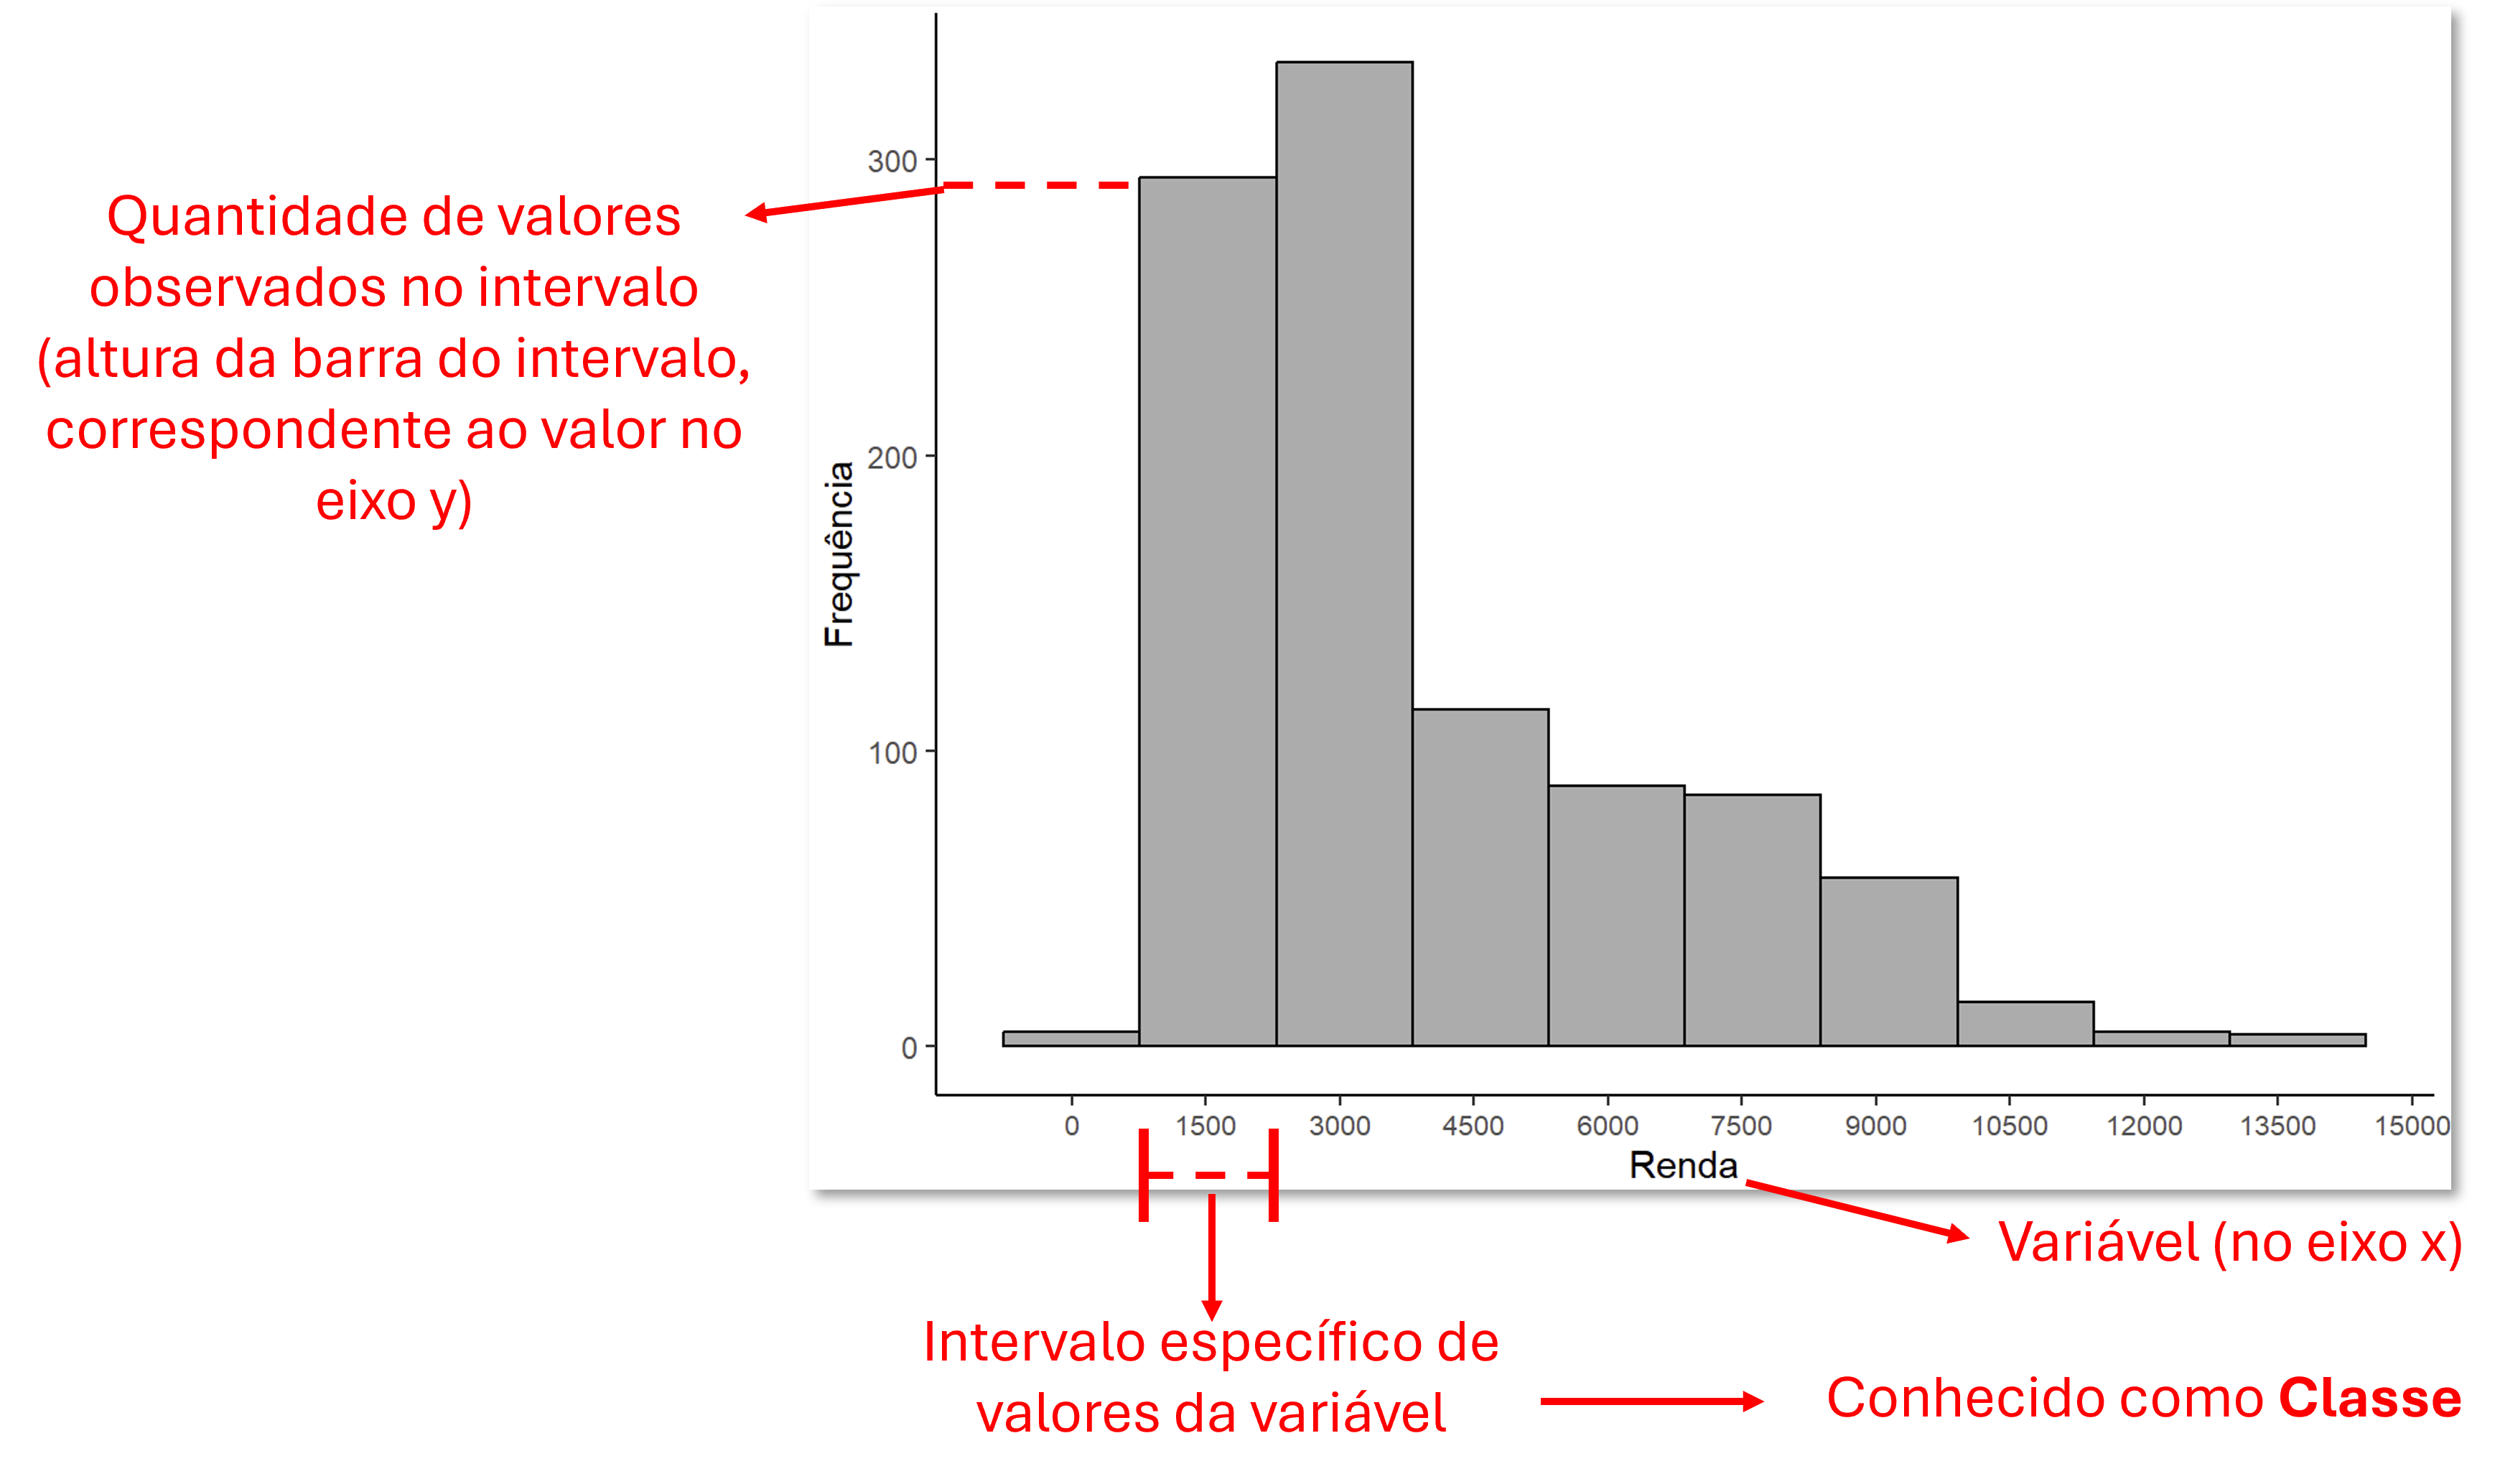
\includegraphics[keepaspectratio]{img/4-visualizacao-de-dados-tabulares/4-12-hist_elementos.png}}

}

\end{figure}%

A leitura de um histograma responde a duas perguntas de imediato. A
primeira é onde os dados se concentram, indicada pelas barras mais
altas. A segunda é quão espalhados eles estão, indicada pela largura da
região ocupada pelas barras.

Para entender como o histograma é montado, é importante interpretar as
escolhas que os pacotes fazem por nós. Vamos construir um manualmente a
partir dos seguintes valores de idade abaixo:

\begin{Shaded}
\begin{Highlighting}[]
\NormalTok{idades }\OtherTok{\textless{}{-}} \FunctionTok{c}\NormalTok{(}\FloatTok{58.8}\NormalTok{, }\FloatTok{65.5}\NormalTok{, }\FloatTok{42.9}\NormalTok{, }\FloatTok{98.4}\NormalTok{, }\FloatTok{87.0}\NormalTok{, }\FloatTok{63.9}\NormalTok{, }\FloatTok{60.8}\NormalTok{, }\FloatTok{60.2}\NormalTok{, }\FloatTok{66.9}\NormalTok{, }\FloatTok{73.8}\NormalTok{,}
            \FloatTok{77.6}\NormalTok{, }\FloatTok{39.9}\NormalTok{, }\FloatTok{58.1}\NormalTok{, }\FloatTok{58.2}\NormalTok{, }\FloatTok{56.5}\NormalTok{, }\FloatTok{59.9}\NormalTok{, }\FloatTok{59.7}\NormalTok{, }\FloatTok{52.8}\NormalTok{, }\FloatTok{62.6}\NormalTok{, }\FloatTok{68.5}\NormalTok{)}
\end{Highlighting}
\end{Shaded}

O primeiro passo é ordenar as idades de forma crescente, o que já dá uma
primeira noção de como elas se distribuem:

\begin{Shaded}
\begin{Highlighting}[]
\FunctionTok{sort}\NormalTok{(idades)}
\end{Highlighting}
\end{Shaded}

\begin{verbatim}
 [1] 39.9 42.9 52.8 56.5 58.1 58.2 58.8 59.7 59.9 60.2 60.8 62.6 63.9 65.5 66.9
[16] 68.5 73.8 77.6 87.0 98.4
\end{verbatim}

O segundo passo é definir as classes. É importante salientar que podemos
escolher a quantidade de classes arbitrariamente, mas que existem regras
práticas úteis para determiná-la. Antes de apresentar estas regras,
vamos salvar alguns valores importantes para esta definição, que são a
quantidade de observações da variável (\(n\)) e sua amplitude:

\begin{Shaded}
\begin{Highlighting}[]
\NormalTok{n }\OtherTok{\textless{}{-}} \FunctionTok{length}\NormalTok{(idades)}

\NormalTok{n}
\end{Highlighting}
\end{Shaded}

\begin{verbatim}
[1] 20
\end{verbatim}

\begin{Shaded}
\begin{Highlighting}[]
\NormalTok{amplitude }\OtherTok{\textless{}{-}} \FunctionTok{max}\NormalTok{(idades) }\SpecialCharTok{{-}} \FunctionTok{min}\NormalTok{(idades)}

\NormalTok{amplitude}
\end{Highlighting}
\end{Shaded}

\begin{verbatim}
[1] 58.5
\end{verbatim}

As duas regras práticas mais difundidas para a determinação da
quantidade de classes (\(C\)) são a raiz quadrada do número de
observações (\(C=\sqrt{n}\)), e a segunda é a regra de Sturges, que
calcula \(C = 1 + \log_2(n)\). Sendo assim:

\begin{Shaded}
\begin{Highlighting}[]
\CommentTok{\# Regra da raiz quadrada:}
\NormalTok{n\_classes\_raizquad }\OtherTok{=} \FunctionTok{sqrt}\NormalTok{(n)}

\NormalTok{n\_classes\_raizquad}
\end{Highlighting}
\end{Shaded}

\begin{verbatim}
[1] 4.472136
\end{verbatim}

\begin{Shaded}
\begin{Highlighting}[]
\CommentTok{\# Regra de Sturges:}
\NormalTok{n\_classes\_rsturges }\OtherTok{=} \DecValTok{1} \SpecialCharTok{+} \FunctionTok{log2}\NormalTok{(n)}

\NormalTok{n\_classes\_rsturges}
\end{Highlighting}
\end{Shaded}

\begin{verbatim}
[1] 5.321928
\end{verbatim}

Em geral, adotamos uma das regras e tomamos o valor do inteiro superior
mais próximo. Neste caso, teríamos o valor de 5 para a regra da raiz
quadrada e 6 para a regra de Sturges. Como ambas apontam para um
resultado em torno de 5, utilizaremos essa quantidade. Logo, dividindo a
amplitude por esse número e obtemos a extensão de cada intervalo
(classe):

\begin{Shaded}
\begin{Highlighting}[]
\NormalTok{n\_classes }\OtherTok{=} \DecValTok{5}
\NormalTok{ext\_intervalo }\OtherTok{=}\NormalTok{ amplitude }\SpecialCharTok{/}\NormalTok{ n\_classes}

\NormalTok{ext\_intervalo}
\end{Highlighting}
\end{Shaded}

\begin{verbatim}
[1] 11.7
\end{verbatim}

O valor de 11,7 anos pode ser pouco prático como referência de leitura,
e por isso costumamos arredondar para um número inteiro superior.
Adotando intervalos de 12 anos iniciadas em 39, os limites das cinco
classes ficam assim:

\begin{Shaded}
\begin{Highlighting}[]
\CommentTok{\# Usamos celing() para obter o maior inteiro (arredondamento p/ cima):}
\NormalTok{ext\_intervalo }\OtherTok{\textless{}{-}} \FunctionTok{ceiling}\NormalTok{(ext\_intervalo) }

\NormalTok{ext\_intervalo}
\end{Highlighting}
\end{Shaded}

\begin{verbatim}
[1] 12
\end{verbatim}

\begin{Shaded}
\begin{Highlighting}[]
\CommentTok{\# Para obter o limite superior do intervalo, somamos o valor mínimo de idade à nova }
\CommentTok{\# amplitude, dada pela extensão do intervalo de uma classe vezes o número de classes:}
\NormalTok{lim\_superior }\OtherTok{\textless{}{-}}\NormalTok{ ext\_intervalo}\SpecialCharTok{*}\NormalTok{n\_classes }\SpecialCharTok{+} \FunctionTok{min}\NormalTok{(idades)}

\NormalTok{lim\_superior}
\end{Highlighting}
\end{Shaded}

\begin{verbatim}
[1] 99.9
\end{verbatim}

\begin{Shaded}
\begin{Highlighting}[]
\CommentTok{\# O código abaixo produz uma sequência numérica começando em \textquotesingle{}from\textquotesingle{}, }
\CommentTok{\# terminando em \textquotesingle{}to\textquotesingle{} e espaçado de \textquotesingle{}by\textquotesingle{} em \textquotesingle{}by\textquotesingle{}:}
\NormalTok{limites }\OtherTok{\textless{}{-}} \FunctionTok{seq}\NormalTok{(}\AttributeTok{from =} \DecValTok{39}\NormalTok{, }\AttributeTok{to =}\NormalTok{ lim\_superior, }\AttributeTok{by =} \DecValTok{12}\NormalTok{) }

\NormalTok{limites}
\end{Highlighting}
\end{Shaded}

\begin{verbatim}
[1] 39 51 63 75 87 99
\end{verbatim}

A convenção usual é tratar cada intervalo como fechado no início e
aberto no final, de modo que a primeira classe contém os valores maiores
ou iguais a 39 anos e menores que 51 anos. No R, a função \texttt{cut()}
faz esse recorte e o argumento \texttt{right\ =\ FALSE} estabelece
justamente essa convenção. O terceiro passo é contar quantas observações
caem em cada classe:

\begin{table}

\caption{\label{tbl-classes}Distribuição de frequências das idades em
cinco classes de 12 anos.}

\centering{

\begin{Shaded}
\begin{Highlighting}[]
\NormalTok{tab\_classes }\OtherTok{\textless{}{-}} \FunctionTok{tibble}\NormalTok{(}\AttributeTok{idades =}\NormalTok{ idades) }\SpecialCharTok{|\textgreater{}}
  \FunctionTok{mutate}\NormalTok{(}\AttributeTok{classe =} \FunctionTok{cut}\NormalTok{(idades, }\AttributeTok{breaks =}\NormalTok{ limites, }\AttributeTok{right =} \ConstantTok{FALSE}\NormalTok{)) }\SpecialCharTok{|\textgreater{}}
  \FunctionTok{count}\NormalTok{(classe, }\AttributeTok{name =} \StringTok{"frequencia"}\NormalTok{) }\SpecialCharTok{|\textgreater{}}
  \FunctionTok{mutate}\NormalTok{(}\AttributeTok{proporcao =}\NormalTok{ frequencia }\SpecialCharTok{/} \FunctionTok{sum}\NormalTok{(frequencia))}

\NormalTok{tab\_classes}
\end{Highlighting}
\end{Shaded}

\begin{verbatim}
# A tibble: 5 x 3
  classe  frequencia proporcao
  <fct>        <int>     <dbl>
1 [39,51)          2      0.1 
2 [51,63)         10      0.5 
3 [63,75)          5      0.25
4 [75,87)          1      0.05
5 [87,99)          2      0.1 
\end{verbatim}

}

\end{table}%

Vamos agora salvar as idades em um formato \texttt{tibble} com única
coluna, já que não podemos passar um vetor para o ggplot:

\begin{Shaded}
\begin{Highlighting}[]
\NormalTok{tab\_idades }\OtherTok{\textless{}{-}} \FunctionTok{tibble}\NormalTok{(}\AttributeTok{idades =}\NormalTok{ idades)}

\NormalTok{tab\_idades}
\end{Highlighting}
\end{Shaded}

\begin{verbatim}
# A tibble: 20 x 1
   idades
    <dbl>
 1   58.8
 2   65.5
 3   42.9
 4   98.4
 5   87  
 6   63.9
 7   60.8
 8   60.2
 9   66.9
10   73.8
11   77.6
12   39.9
13   58.1
14   58.2
15   56.5
16   59.9
17   59.7
18   52.8
19   62.6
20   68.5
\end{verbatim}

O quarto e último passo é desenhar uma barra para cada classe, com
altura igual à sua frequência. É exatamente o que o
\texttt{geom\_histogram()} faz:

\begin{Shaded}
\begin{Highlighting}[]
\NormalTok{tab\_idades }\SpecialCharTok{|\textgreater{}}
  \FunctionTok{ggplot}\NormalTok{(}\FunctionTok{aes}\NormalTok{(}\AttributeTok{x =}\NormalTok{ idades)) }\SpecialCharTok{+}
  \FunctionTok{geom\_histogram}\NormalTok{()}
\end{Highlighting}
\end{Shaded}

\begin{verbatim}
`stat_bin()` using `bins = 30`. Pick better value `binwidth`.
\end{verbatim}

\begin{figure}[H]

\caption{\label{fig-hist-manual}Histograma das idades com o número de
classes definido automaticamente pelo \texttt{ggplot2}.}

\centering{

\pandocbounded{
\includegraphics[keepaspectratio]{4-visualizacao-de-dados-tabulares_files/figure-pdf/fig-hist-manual-1.pdf}}

}

\end{figure}%

Observe a mensagem reproduzida logo acima do gráfico. Ela indica que o
\texttt{ggplot2} adotou 30 classes (\emph{bins}) por padrão e nos sugere
escolher um número mais apropriado. Podemos então informar no argumento
\texttt{bins} a quantidade de classes que calculamos anteriormente
(\texttt{n\_classes}), conforme o exemplo abaixo:

\begin{Shaded}
\begin{Highlighting}[]
\NormalTok{tab\_idades }\SpecialCharTok{|\textgreater{}}
  \FunctionTok{ggplot}\NormalTok{(}\FunctionTok{aes}\NormalTok{(}\AttributeTok{x =}\NormalTok{ idades)) }\SpecialCharTok{+}
  \FunctionTok{geom\_histogram}\NormalTok{(}\AttributeTok{bins =}\NormalTok{ n\_classes)}
\end{Highlighting}
\end{Shaded}

\begin{figure}[H]

\caption{\label{fig-hist-bins}Histograma das idades com o número de
classes definido pelo argumento \texttt{bins}.}

\centering{

\pandocbounded{
\includegraphics[keepaspectratio]{4-visualizacao-de-dados-tabulares_files/figure-pdf/fig-hist-bins-1.pdf}}

}

\end{figure}%

O gráfico passou a ter cinco barras, como queríamos, mas os limites das
classes não são os mesmos da Tabela~\ref{tbl-classes}. A primeira barra
começa em 32,6 anos e cada classe tem extensão de 14,6 anos, e não os 12
anos que havíamos definido. Isso ocorre porque o
\texttt{geom\_histogram()} do \texttt{ggplot2} usa uma lógica específica
para definir os limites das classes (\emph{bins}) quando o argumento
\texttt{bins} é ajustado. Ao contrário do que se poderia esperar, ele
não divide o intervalo total dos dados pelo número de classes, e sim por
esse número menos um. O motivo é que o \texttt{ggplot2} posiciona as
classes de forma que a primeira fique centrada no valor mínimo e a
última no valor máximo, o que faz sobrar meia classe em cada
extremidade. Com dados de 0 a 100 e \texttt{bins\ =\ 5}, por exemplo,
cada classe terá extensão de 25 unidades (e não 20), e o histograma se
estenderá de -12,5 a 112,5. No nosso caso, a amplitude de 58,5 anos foi
dividida por 4, o que produziu as classes de 14,6 anos que observamos.
Por esse motivo, quando os limites das classes forem importantes, convém
defini-los diretamente, como faremos a seguir com o argumento de
extensão da classe \texttt{binwidth}.

Abaixo passamos a esse argumento o valor \texttt{ext\_intervalo} que
calculamos anteriormente:

\begin{Shaded}
\begin{Highlighting}[]
\NormalTok{tab\_idades }\SpecialCharTok{|\textgreater{}}
  \FunctionTok{ggplot}\NormalTok{(}\FunctionTok{aes}\NormalTok{(}\AttributeTok{x =}\NormalTok{ idades)) }\SpecialCharTok{+}
  \FunctionTok{geom\_histogram}\NormalTok{(}\AttributeTok{binwidth =}\NormalTok{ ext\_intervalo)}
\end{Highlighting}
\end{Shaded}

\begin{figure}[H]

\caption{\label{fig-hist-binwidth}Histograma das idades com a extensão
das classes definida pelo argumento \texttt{binwidth}.}

\centering{

\pandocbounded{
\includegraphics[keepaspectratio]{4-visualizacao-de-dados-tabulares_files/figure-pdf/fig-hist-binwidth-1.pdf}}

}

\end{figure}%

Cada classe tem agora os 12 anos de extensão que pedimos, mas o
resultado continua diferente da Tabela~\ref{tbl-classes}, porque
surgiram seis barras em vez de cinco. Isso acontece porque o
\texttt{binwidth} define a largura das classes sem dizer onde a primeira
delas começa, e o \texttt{ggplot2} a iniciou em 30 anos. Para chegar ao
mesmo recorte da tabela precisamos de mais dois argumentos. O
\texttt{boundary} fixa um dos limites das classes, e o \texttt{closed}
estabelece se os intervalos são fechados à esquerda ou à direita,
cumprindo o mesmo papel do argumento \texttt{right} da função
\texttt{cut()} que usamos antes:

\begin{Shaded}
\begin{Highlighting}[]
\NormalTok{tab\_idades }\SpecialCharTok{|\textgreater{}}
  \FunctionTok{ggplot}\NormalTok{(}\FunctionTok{aes}\NormalTok{(}\AttributeTok{x =}\NormalTok{ idades)) }\SpecialCharTok{+}
  \FunctionTok{geom\_histogram}\NormalTok{(}\AttributeTok{binwidth =}\NormalTok{ ext\_intervalo, }\AttributeTok{boundary =} \DecValTok{39}\NormalTok{, }\AttributeTok{closed =} \StringTok{"left"}\NormalTok{)}
\end{Highlighting}
\end{Shaded}

\begin{figure}[H]

\caption{\label{fig-hist-boundary}Histograma das idades com largura,
origem e fechamento das classes definidos explicitamente.}

\centering{

\pandocbounded{
\includegraphics[keepaspectratio]{4-visualizacao-de-dados-tabulares_files/figure-pdf/fig-hist-boundary-1.pdf}}

}

\end{figure}%

Com os três argumentos combinados, o histograma finalmente reproduz as
frequências da Tabela~\ref{tbl-classes}. Vale registrar que esse nível
de controle raramente é necessário na prática, já que na maior parte das
vezes basta ajustar \texttt{bins} ou \texttt{binwidth} até que a forma
da distribuição fique legível. Ele é útil, porém, quando o histograma
precisa corresponder a classes definidas por alguma convenção externa,
como faixas etárias oficiais ou faixas de renda em salários mínimos.

Neste momento é interessante testar algumas edições ao nosso gráfico que
podem torná-los mais visualmente adequados. No código abaixo, nós
reescrevemos os nomes dos eixos \(x\) e \(y\), além de propor um título
(\texttt{title}), um subtítulo (\texttt{subtitle}) e uma legenda para o
gráfico (\texttt{caption}) por meio da função \texttt{labs()}:

\begin{Shaded}
\begin{Highlighting}[]
\NormalTok{tab\_idades }\SpecialCharTok{|\textgreater{}}
  \FunctionTok{ggplot}\NormalTok{(}\FunctionTok{aes}\NormalTok{(}\AttributeTok{x =}\NormalTok{ idades)) }\SpecialCharTok{+}
  \FunctionTok{geom\_histogram}\NormalTok{(}\AttributeTok{bins =}\NormalTok{ n\_classes) }\SpecialCharTok{+}
  \FunctionTok{labs}\NormalTok{(}\AttributeTok{x =} \StringTok{"Idade"}\NormalTok{, }\AttributeTok{y =} \StringTok{"Frequência"}\NormalTok{, }\AttributeTok{title =} \StringTok{"Histograma"}\NormalTok{, }\AttributeTok{subtitle =} \StringTok{"Idades"}\NormalTok{,}
       \AttributeTok{caption =} \StringTok{"Nota: Valores extraídos de uma base de dados sobre estudos etários"}\NormalTok{)}
\end{Highlighting}
\end{Shaded}

\begin{figure}[H]

\caption{\label{fig-hist-labs}Histograma das idades com título,
subtítulo e nota definidos por \texttt{labs()}.}

\centering{

\pandocbounded{
\includegraphics[keepaspectratio]{4-visualizacao-de-dados-tabulares_files/figure-pdf/fig-hist-labs-1.pdf}}

}

\end{figure}%

A aparência das barras também pode ajustada pelos argumentos
\texttt{color}, que define a cor do contorno, \texttt{fill}, que define
a cor de preenchimento, e \texttt{alpha}, que define a opacidade entre 0
e 1:

\begin{Shaded}
\begin{Highlighting}[]
\NormalTok{tab\_idades }\SpecialCharTok{|\textgreater{}}
  \FunctionTok{ggplot}\NormalTok{(}\FunctionTok{aes}\NormalTok{(}\AttributeTok{x =}\NormalTok{ idades)) }\SpecialCharTok{+}
  \FunctionTok{geom\_histogram}\NormalTok{(}\AttributeTok{bins =}\NormalTok{ n\_classes, }\AttributeTok{color =} \StringTok{"black"}\NormalTok{,}
                 \AttributeTok{fill =} \StringTok{"steelblue"}\NormalTok{, }\AttributeTok{alpha =} \FloatTok{0.4}\NormalTok{) }\SpecialCharTok{+}
  \FunctionTok{labs}\NormalTok{(}\AttributeTok{x =} \StringTok{"Idade"}\NormalTok{, }\AttributeTok{y =} \StringTok{"Frequência"}\NormalTok{,}
       \AttributeTok{title =} \StringTok{"Histograma"}\NormalTok{, }\AttributeTok{subtitle =} \StringTok{"Idades"}\NormalTok{,}
       \AttributeTok{caption =} \StringTok{"Nota: Valores extraídos de uma base de dados sobre estudos etários"}\NormalTok{)}
\end{Highlighting}
\end{Shaded}

\begin{figure}[H]

\caption{\label{fig-hist-cores}Histograma das idades com ajustes de
contorno, preenchimento e opacidade das barras.}

\centering{

\pandocbounded{
\includegraphics[keepaspectratio]{4-visualizacao-de-dados-tabulares_files/figure-pdf/fig-hist-cores-1.pdf}}

}

\end{figure}%

Uma observação interessante é que as cores de contorno e preenchimento
podem ser definidas tanto por nomes (como o ``black'' e o
``steelblue''), quanto por meio de códigos de cor hexadecimal. Uma fonte
interessante para obter esses códigos é o site
\href{https://htmlcolorcodes.com/}{HTML Color Codes}. Experimente por
exemplo o gráfico anterior com \texttt{color\ =\ \#E8A61A} e
\texttt{fill\ =\ \#F50C05}.

\begin{tcolorbox}[enhanced jigsaw, arc=.35mm, bottomrule=.15mm, bottomtitle=1mm, breakable, colback=white, colbacktitle=quarto-callout-note-color!10!white, colframe=quarto-callout-note-color-frame, coltitle=black, left=2mm, leftrule=.75mm, opacityback=0, opacitybacktitle=0.6, rightrule=.15mm, title=\textcolor{quarto-callout-note-color}{\faInfo}\hspace{0.5em}{Argumentos dentro e fora de \texttt{aes()}}, titlerule=0mm, toprule=.15mm, toptitle=1mm]

Note que os argumentos \texttt{color}, \texttt{fill} e \texttt{alpha}
acima estão fora de \texttt{aes()}, e por isso não são mapeamento
estético. Eles atribuem um valor fixo à geometria inteira. Quando esses
mesmos argumentos aparecem dentro de \texttt{aes()}, passam a
representar uma variável da base, e o \texttt{ggplot2} cria
automaticamente uma escala e uma legenda para eles. Essa distinção
percorre todo o restante do capítulo.

\end{tcolorbox}

A última camada que costumamos ajustar é o tema. O \texttt{ggplot2} traz
vários temas prontos, entre eles \texttt{theme\_bw()},
\texttt{theme\_minimal()}, \texttt{theme\_classic()} e
\texttt{theme\_void()}, que alteram cores de fundo, grades e eixos sem
tocar nos dados representados. Abaixo testaremos o tema
\texttt{theme\_bw()}, mas fique à vontade para testar os possíveis temas
pré-definidos do \texttt{ggplot2}:

\begin{Shaded}
\begin{Highlighting}[]
\NormalTok{tab\_idades }\SpecialCharTok{|\textgreater{}}
  \FunctionTok{ggplot}\NormalTok{(}\FunctionTok{aes}\NormalTok{(}\AttributeTok{x =}\NormalTok{ idades)) }\SpecialCharTok{+}
  \FunctionTok{geom\_histogram}\NormalTok{(}\AttributeTok{bins =}\NormalTok{ n\_classes, }\AttributeTok{color =} \StringTok{"black"}\NormalTok{,}
                 \AttributeTok{fill =} \StringTok{"steelblue"}\NormalTok{, }\AttributeTok{alpha =} \FloatTok{0.4}\NormalTok{) }\SpecialCharTok{+}
  \FunctionTok{labs}\NormalTok{(}\AttributeTok{x =} \StringTok{"Idade"}\NormalTok{, }\AttributeTok{y =} \StringTok{"Frequência"}\NormalTok{,}
       \AttributeTok{title =} \StringTok{"Histograma"}\NormalTok{, }\AttributeTok{subtitle =} \StringTok{"Idades"}\NormalTok{,}
       \AttributeTok{caption =} \StringTok{"Nota: Valores extraídos de uma base de dados sobre estudos etários"}\NormalTok{) }\SpecialCharTok{+}
  \FunctionTok{theme\_bw}\NormalTok{()}
\end{Highlighting}
\end{Shaded}

\begin{figure}[H]

\caption{\label{fig-hist-tema}Histograma das idades com o tema
\texttt{theme\_bw()} aplicado.}

\centering{

\pandocbounded{
\includegraphics[keepaspectratio]{4-visualizacao-de-dados-tabulares_files/figure-pdf/fig-hist-tema-1.pdf}}

}

\end{figure}%

\subsection{\texorpdfstring{O
\emph{boxplot}}{O boxplot}}\label{o-boxplot}

O diagrama de caixa, mais conhecido como \emph{boxplot}, também é
utilizado para representar a distribuição dos dados. Há, porém, um ganho
adicional em relação ao histograma, ao permitir identificar algumas
medidas de posição importantes a partir do seu desenho. Ele é composto
por uma caixa, dois traços que dela se estendem, chamados
\emph{whiskers}, e eventualmente por pontos isolados, conforme podemos
observar na Figura~\ref{fig-boxplot-elementos}.

\begin{figure}[H]

\caption{\label{fig-boxplot-elementos}Anatomia de um boxplot, com a
caixa delimitada por Q1 e Q3, a mediana (Q2) em seu interior, os
\emph{whiskers} e os \emph{outliers}. Fonte: adaptado de Irizarry (s.
d.).}

\centering{

\pandocbounded{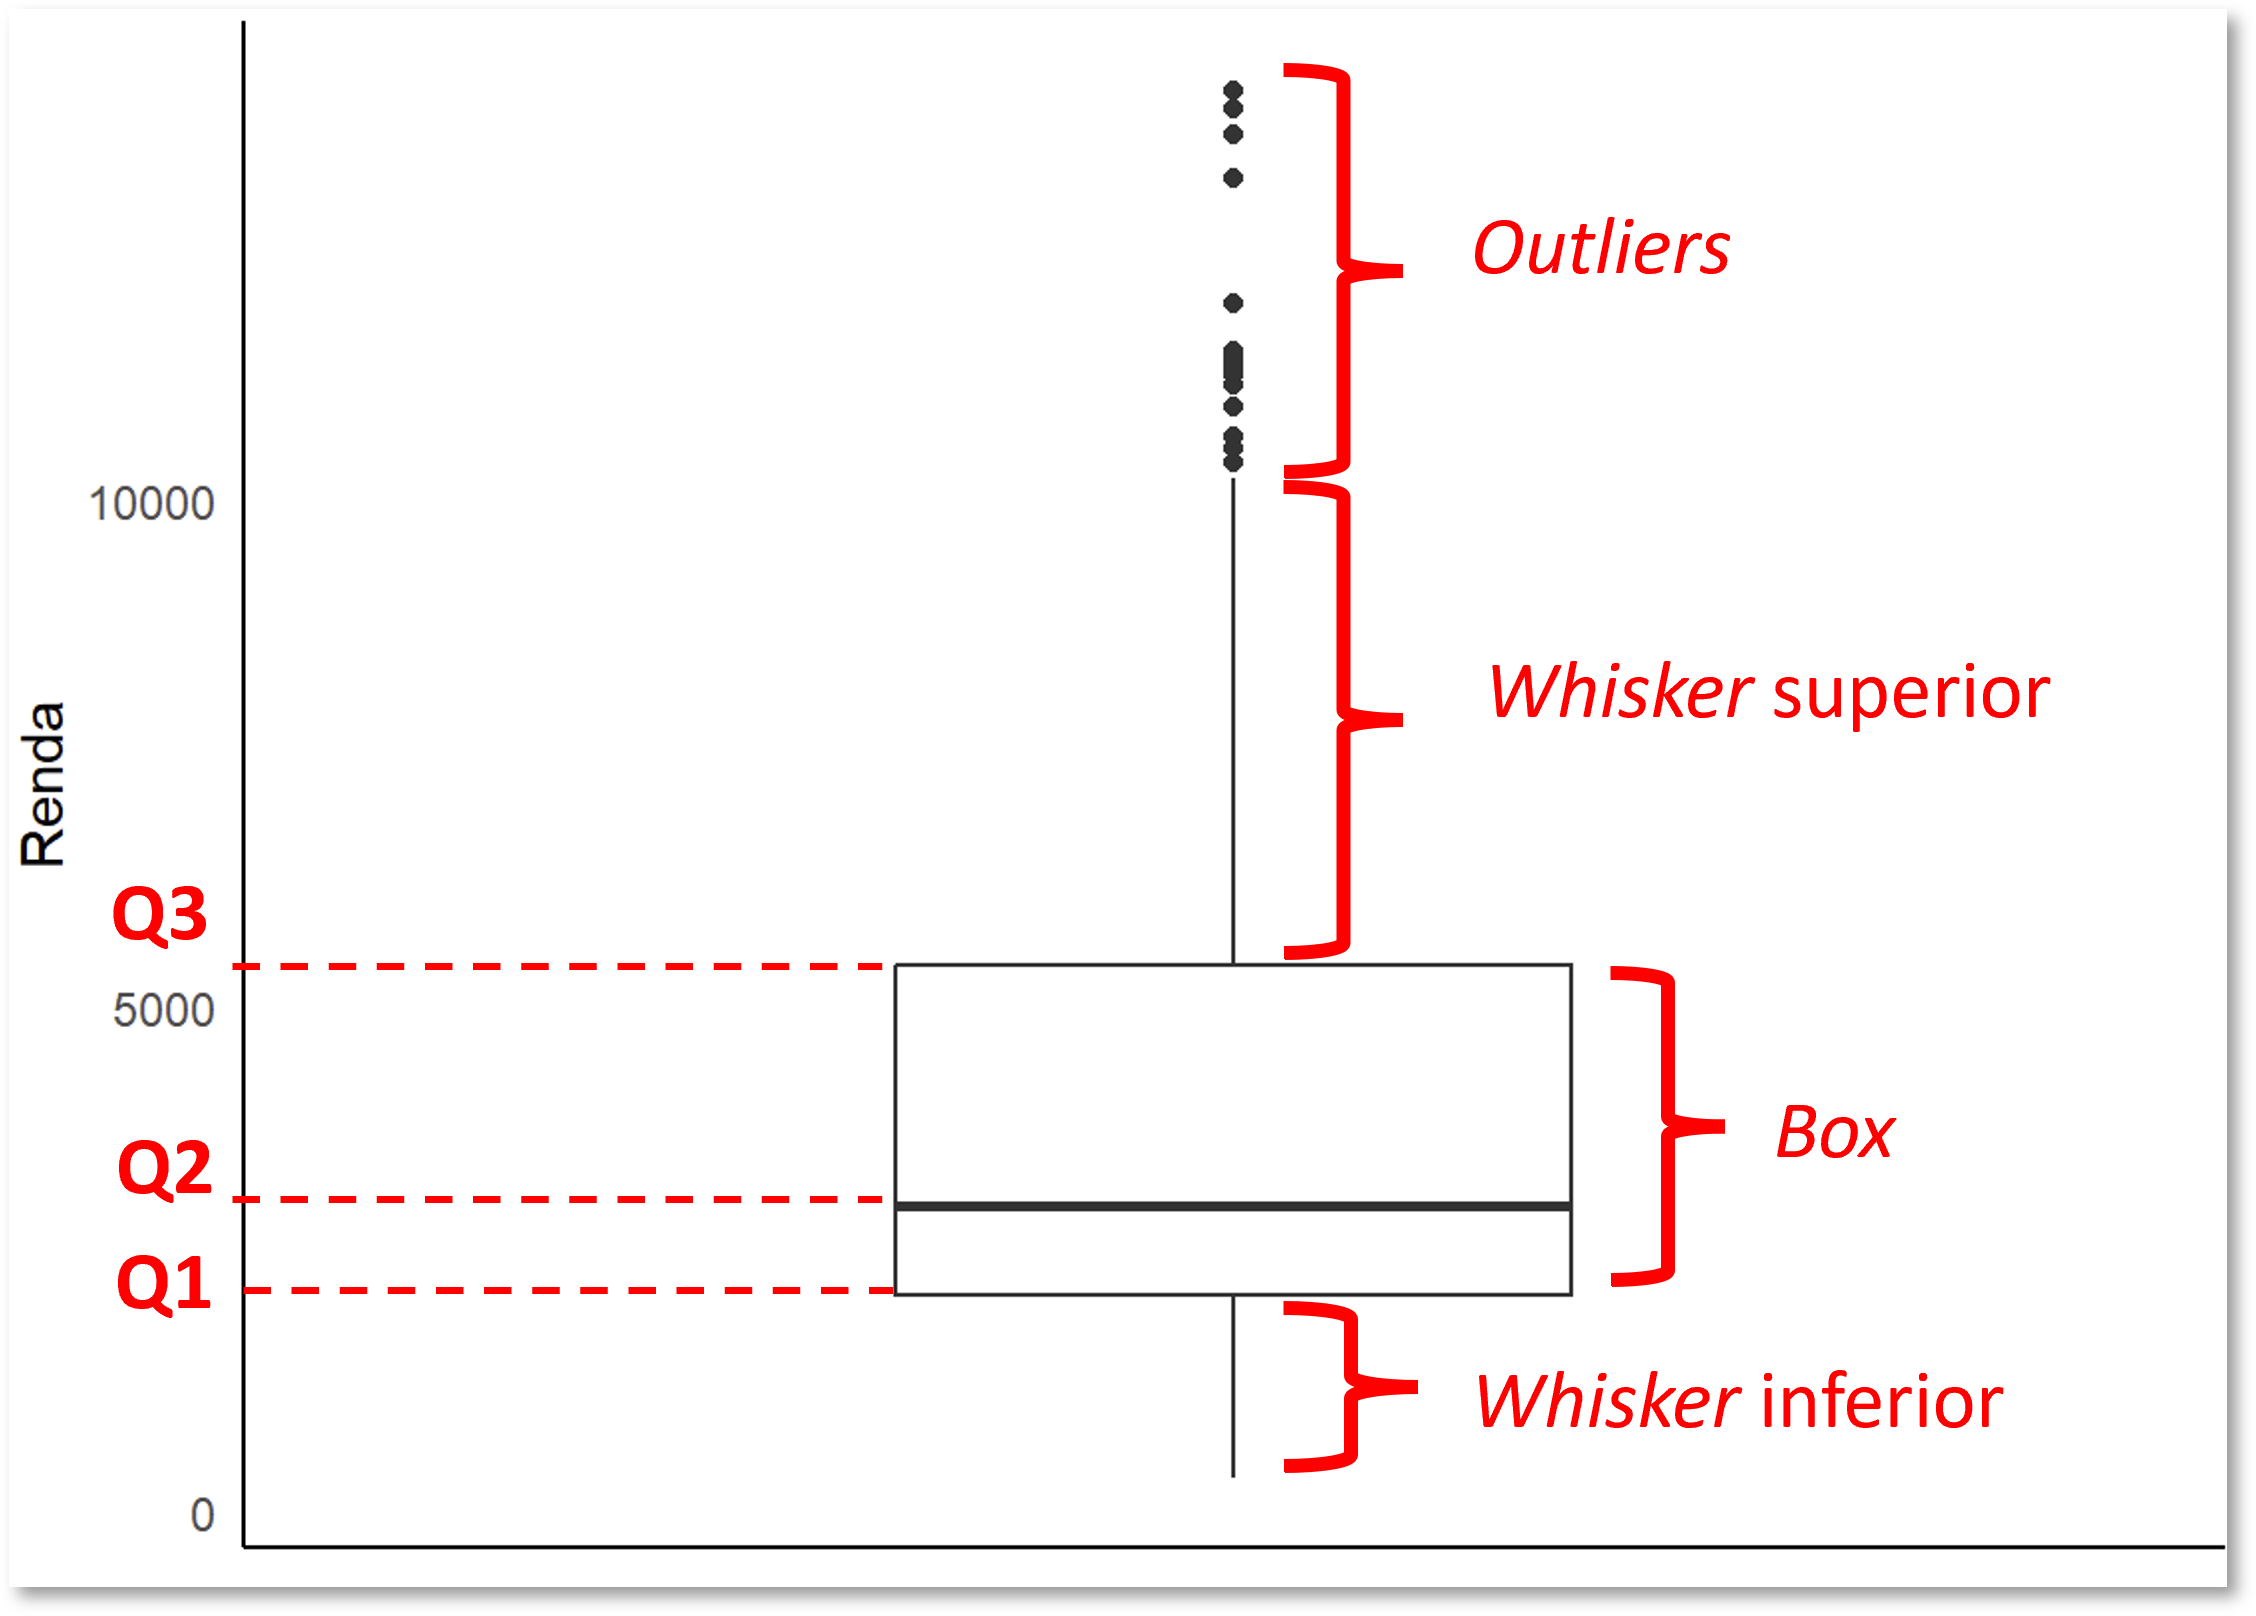
\includegraphics[keepaspectratio]{img/4-visualizacao-de-dados-tabulares/4-20-boxplot_elementos.png}}

}

\end{figure}%

A caixa é delimitada pelo primeiro e pelo terceiro quartis, com um traço
interno na mediana. Ela contém, portanto, os 50\% centrais das
observações, e quanto menor sua altura maior é a concentração no centro
da distribuição. Os \emph{whiskers} se estendem até o valor mais extremo
que ainda esteja a até 1,5 intervalo interquartil \((IQR = Q3 - Q1)\) de
distância da caixa. Isso significa que o \emph{whisker}
\textbf{superior} se estende até o \textbf{menor} valor entre
\(\max{x}\) e \(Q3 + 1{,}5 \cdot IQR\) e o \emph{whisker}
\textbf{inferior} se estende até o \textbf{maior} valor entre
\(\min{x}\) e \(Q1 - 1{,}5 \cdot IQR\). Observações além desses limites
(para cima ou para baixo) são desenhadas individualmente e classificadas
como valores discrepantes ou \emph{outliers}\footnote{É também comum
  utilizar o multiplicador 3 para a definição, ou seja
  \(Q3 + 3 \cdot IQR\) e \(Q1 - 3 \cdot IQR\)}, sendo pontos de atenção
no controle de qualidade dos dados.

Voltemos aos dados de \texttt{em}. Para construir um \emph{boxplot} da
renda, mapeamos a variável ao eixo vertical e adicionamos
\texttt{geom\_boxplot()}:

\begin{Shaded}
\begin{Highlighting}[]
\NormalTok{em }\SpecialCharTok{|\textgreater{}}
  \FunctionTok{ggplot}\NormalTok{(}\FunctionTok{aes}\NormalTok{(}\AttributeTok{y =}\NormalTok{ renda)) }\SpecialCharTok{+}
  \FunctionTok{geom\_boxplot}\NormalTok{() }\SpecialCharTok{+}
  \FunctionTok{labs}\NormalTok{(}\AttributeTok{y =} \StringTok{"Renda (R$)"}\NormalTok{) }\SpecialCharTok{+}
  \FunctionTok{theme\_bw}\NormalTok{()}
\end{Highlighting}
\end{Shaded}

\begin{figure}[H]

\caption{\label{fig-boxplot-renda}Boxplot da renda dos entrevistados.}

\centering{

\pandocbounded{
\includegraphics[keepaspectratio]{4-visualizacao-de-dados-tabulares_files/figure-pdf/fig-boxplot-renda-1.pdf}}

}

\end{figure}%

Quando representamos a distribuição de uma única variável, a caixa ocupa
toda a largura disponível, o que é pouco elegante. Como o
\texttt{ggplot2} posiciona a caixa entre -0,4 e 0,4 no eixo
horizontal\footnote{Note que esses valores no eixo \(x\) não possuem
  qualquer significado em relação à base de dados, pois servem somente
  para posicionarmos a caixa}, basta ampliar os limites desse eixo com
\texttt{xlim()} para obter uma proporção mais agradável:

\begin{Shaded}
\begin{Highlighting}[]
\NormalTok{em }\SpecialCharTok{|\textgreater{}}
  \FunctionTok{ggplot}\NormalTok{(}\FunctionTok{aes}\NormalTok{(}\AttributeTok{y =}\NormalTok{ renda)) }\SpecialCharTok{+}
  \FunctionTok{geom\_boxplot}\NormalTok{() }\SpecialCharTok{+}
  \FunctionTok{xlim}\NormalTok{(}\SpecialCharTok{{-}}\DecValTok{1}\NormalTok{, }\DecValTok{1}\NormalTok{) }\SpecialCharTok{+}
  \FunctionTok{labs}\NormalTok{(}\AttributeTok{y =} \StringTok{"Renda (R$)"}\NormalTok{) }\SpecialCharTok{+}
  \FunctionTok{theme\_bw}\NormalTok{()}
\end{Highlighting}
\end{Shaded}

\begin{figure}[H]

\caption{\label{fig-boxplot-ajustado}Boxplot da renda com os limites do
eixo horizontal ajustados.}

\centering{

\pandocbounded{
\includegraphics[keepaspectratio]{4-visualizacao-de-dados-tabulares_files/figure-pdf/fig-boxplot-ajustado-1.pdf}}

}

\end{figure}%

Vale conferir numericamente a que correspondem os elementos do gráfico.
Calculando os quartis, o intervalo interquartil e os limites dos
\emph{whiskers}:

\begin{Shaded}
\begin{Highlighting}[]
\NormalTok{Q1  }\OtherTok{\textless{}{-}} \FunctionTok{quantile}\NormalTok{(em}\SpecialCharTok{$}\NormalTok{renda, }\FloatTok{0.25}\NormalTok{)}
\NormalTok{Q3  }\OtherTok{\textless{}{-}} \FunctionTok{quantile}\NormalTok{(em}\SpecialCharTok{$}\NormalTok{renda, }\FloatTok{0.75}\NormalTok{)}

\NormalTok{Q1; Q3}
\end{Highlighting}
\end{Shaded}

\begin{verbatim}
    25% 
2141.75 
\end{verbatim}

\begin{verbatim}
 75% 
5398 
\end{verbatim}

\begin{Shaded}
\begin{Highlighting}[]
\NormalTok{IQR }\OtherTok{\textless{}{-}}\NormalTok{ Q3 }\SpecialCharTok{{-}}\NormalTok{ Q1}

\NormalTok{IQR}
\end{Highlighting}
\end{Shaded}

\begin{verbatim}
    75% 
3256.25 
\end{verbatim}

\begin{Shaded}
\begin{Highlighting}[]
\FunctionTok{c}\NormalTok{(}\AttributeTok{Q1 =}\NormalTok{ Q1, }\AttributeTok{mediana =} \FunctionTok{median}\NormalTok{(em}\SpecialCharTok{$}\NormalTok{renda), }\AttributeTok{Q3 =}\NormalTok{ Q3, }\AttributeTok{IQR =}\NormalTok{ IQR)}
\end{Highlighting}
\end{Shaded}

\begin{verbatim}
 Q1.25% mediana  Q3.75% IQR.75% 
2141.75 3017.00 5398.00 3256.25 
\end{verbatim}

\begin{Shaded}
\begin{Highlighting}[]
\FunctionTok{c}\NormalTok{(}\AttributeTok{limite\_inferior =}\NormalTok{ Q1 }\SpecialCharTok{{-}} \FloatTok{1.5} \SpecialCharTok{*}\NormalTok{ IQR, }\AttributeTok{minimo =} \FunctionTok{min}\NormalTok{(em}\SpecialCharTok{$}\NormalTok{renda))}
\end{Highlighting}
\end{Shaded}

\begin{verbatim}
limite_inferior.25%              minimo 
          -2742.625             327.000 
\end{verbatim}

\begin{Shaded}
\begin{Highlighting}[]
\FunctionTok{c}\NormalTok{(}\AttributeTok{limite\_superior =}\NormalTok{ Q3 }\SpecialCharTok{+} \FloatTok{1.5} \SpecialCharTok{*}\NormalTok{ IQR, }\AttributeTok{maximo =} \FunctionTok{max}\NormalTok{(em}\SpecialCharTok{$}\NormalTok{renda))}
\end{Highlighting}
\end{Shaded}

\begin{verbatim}
limite_superior.75%              maximo 
           10282.38            14049.00 
\end{verbatim}

O \emph{whisker} inferior termina no valor mínimo observado
(\texttt{min(em\$renda)}), porque este é maior que
\(Q_1 - 1{,}5 \cdot IQR\). Já o \emph{whisker} superior termina antes do
máximo (\texttt{max(em\$renda)}), o que confirma a existência de
observações classificadas como \emph{outliers} na cauda superior da
distribuição de renda.

Observe na Figura~\ref{fig-hist-vs-boxplot} como histograma e boxplot
são complementares. O histograma mostra a forma completa da
distribuição, incluindo eventuais picos, e o boxplot resume posição e
dispersão de maneira compacta, o que o torna especialmente útil para
comparar vários grupos lado a lado. Em uma análise exploratória com
variáveis numéricas é sempre interessante explorar ambos.

\begin{figure}[H]

\caption{\label{fig-hist-vs-boxplot}Dois conjuntos de dados com seus
histogramas e boxplots correspondentes. As duas representações descrevem
a mesma distribuição sob perspectivas diferentes.}

\centering{

\pandocbounded{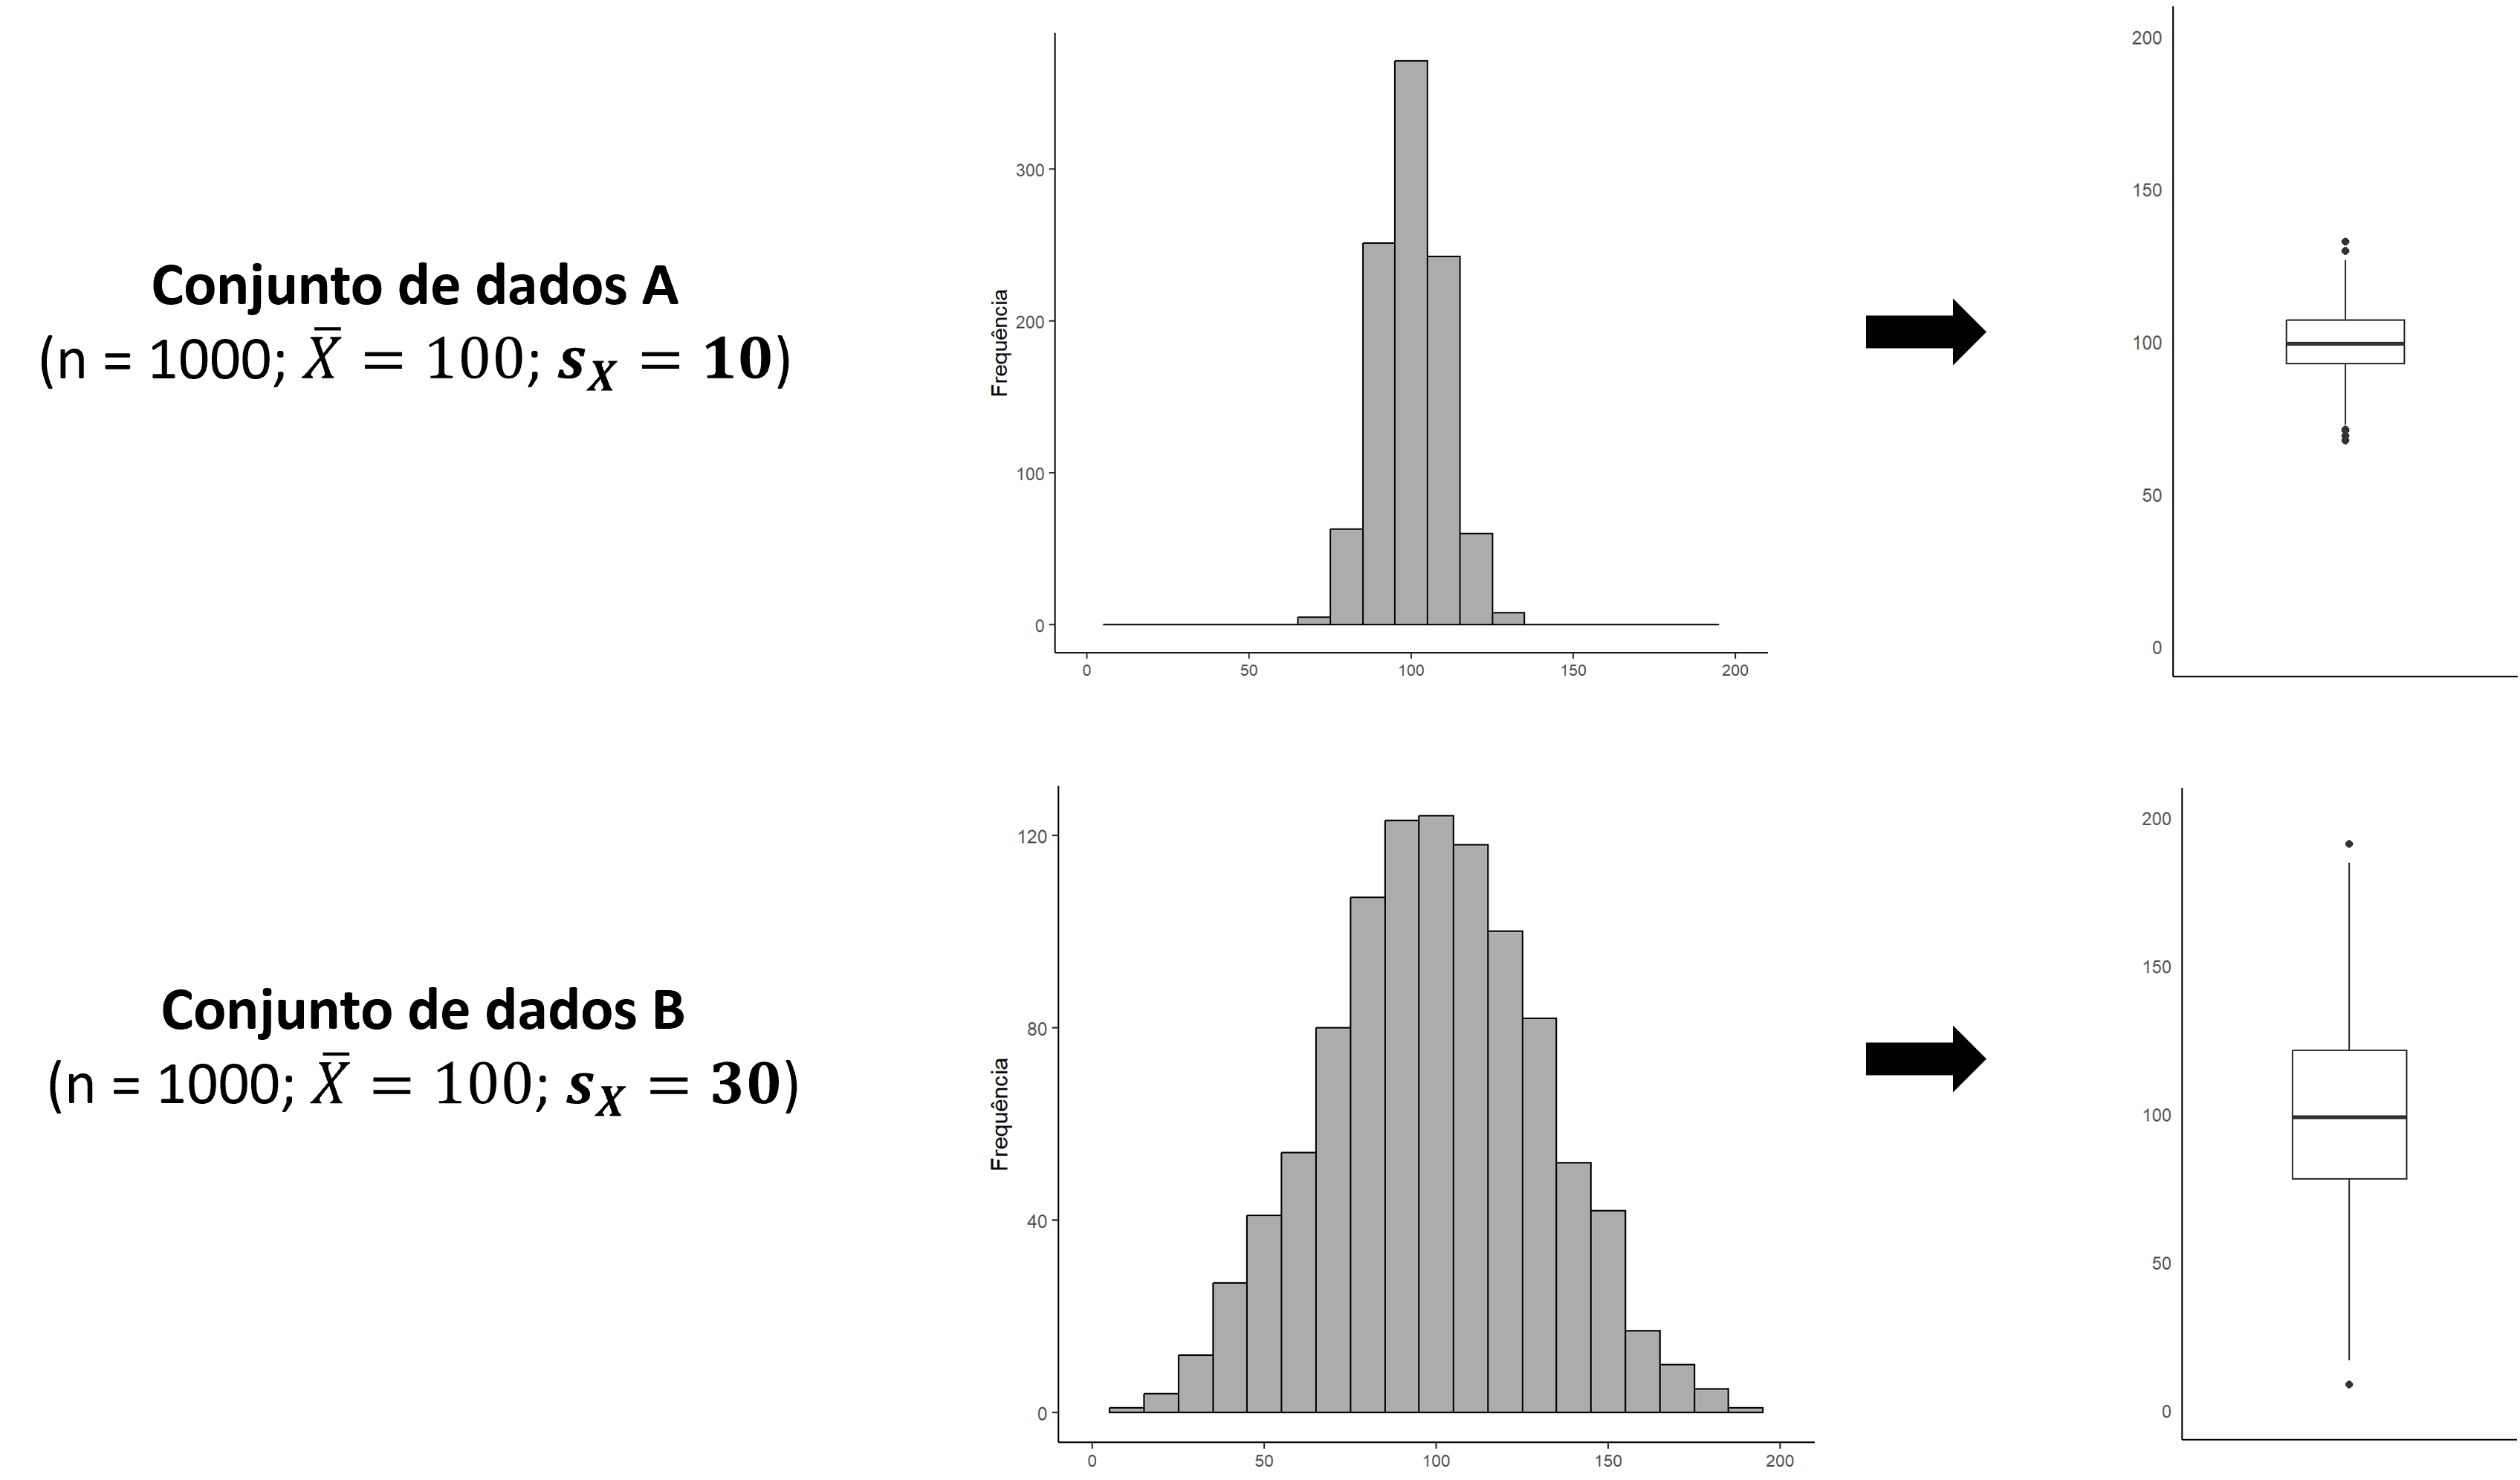
\includegraphics[keepaspectratio]{img/4-visualizacao-de-dados-tabulares/4-23-boxplot_vs_histograma.png}}

}

\end{figure}%

\subsection{O gráfico de barras}\label{o-gruxe1fico-de-barras}

Para variáveis categóricas, a representação usual é o gráfico de barras,
que conta as observações em cada nível. O eixo horizontal traz os níveis
e o eixo vertical traz a contagem, dada pela altura das barras.

O caminho mais direto usa \texttt{geom\_bar()}, que faz a contagem
internamente a partir da base completa:

\begin{Shaded}
\begin{Highlighting}[]
\NormalTok{em }\SpecialCharTok{|\textgreater{}}
  \FunctionTok{ggplot}\NormalTok{(}\FunctionTok{aes}\NormalTok{(}\AttributeTok{x =}\NormalTok{ modo\_viagem)) }\SpecialCharTok{+}
  \FunctionTok{geom\_bar}\NormalTok{() }\SpecialCharTok{+}
  \FunctionTok{labs}\NormalTok{(}\AttributeTok{x =} \StringTok{"Modo de viagem"}\NormalTok{, }\AttributeTok{y =} \StringTok{"Frequência"}\NormalTok{) }\SpecialCharTok{+}
  \FunctionTok{theme\_bw}\NormalTok{()}
\end{Highlighting}
\end{Shaded}

\begin{figure}[H]

\caption{\label{fig-barras-modo}Quantidade de entrevistados por modo de
viagem.}

\centering{

\pandocbounded{
\includegraphics[keepaspectratio]{4-visualizacao-de-dados-tabulares_files/figure-pdf/fig-barras-modo-1.pdf}}

}

\end{figure}%

Um caminho alternativo parte de uma tabela já agregada. Sumarizando
antes com \texttt{count()}, passamos a ter uma coluna com as contagens,
e nesse caso a geometria apropriada é \texttt{geom\_col()}, que usa os
valores tal como estão em vez de contá-los:

\begin{Shaded}
\begin{Highlighting}[]
\NormalTok{tab\_mv }\OtherTok{\textless{}{-}}\NormalTok{ em }\SpecialCharTok{|\textgreater{}}
  \FunctionTok{count}\NormalTok{(modo\_viagem)}

\NormalTok{tab\_mv}
\end{Highlighting}
\end{Shaded}

\begin{verbatim}
# A tibble: 4 x 2
  modo_viagem      n
  <fct>        <int>
1 A pé           150
2 Bicicleta      141
3 Carro ou App   380
4 TP             329
\end{verbatim}

\begin{Shaded}
\begin{Highlighting}[]
\NormalTok{tab\_mv }\SpecialCharTok{|\textgreater{}}
  \FunctionTok{ggplot}\NormalTok{(}\FunctionTok{aes}\NormalTok{(}\AttributeTok{x =}\NormalTok{ modo\_viagem, }\AttributeTok{y =}\NormalTok{ n)) }\SpecialCharTok{+}
  \FunctionTok{geom\_col}\NormalTok{() }\SpecialCharTok{+}
  \FunctionTok{labs}\NormalTok{(}\AttributeTok{x =} \StringTok{"Modo de viagem"}\NormalTok{, }\AttributeTok{y =} \StringTok{"Frequência"}\NormalTok{) }\SpecialCharTok{+}
  \FunctionTok{theme\_bw}\NormalTok{()}
\end{Highlighting}
\end{Shaded}

\begin{figure}[H]

\caption{\label{fig-barras-col}O mesmo gráfico construído a partir de
uma tabela previamente agregada.}

\centering{

\pandocbounded{
\includegraphics[keepaspectratio]{4-visualizacao-de-dados-tabulares_files/figure-pdf/fig-barras-col-1.pdf}}

}

\end{figure}%

Uma terceira forma equivalente é usar o
\texttt{geom\_bar(stat\ =\ "identity")}, notação mais antiga que produz
o mesmo resultado de \texttt{geom\_col()} e ainda aparece com frequência
em códigos R.

Os ajustes visuais seguem uma lógica parecida com a do histograma, com
\texttt{width} controlando a largura das barras, cujo padrão é 0,9.
Quando os rótulos dos níveis são longos, a função \texttt{coord\_flip()}
inverte os eixos e melhora bastante a legibilidade:

\begin{Shaded}
\begin{Highlighting}[]
\NormalTok{em }\SpecialCharTok{|\textgreater{}}
  \FunctionTok{ggplot}\NormalTok{(}\FunctionTok{aes}\NormalTok{(}\AttributeTok{x =}\NormalTok{ modo\_viagem)) }\SpecialCharTok{+}
  \FunctionTok{geom\_bar}\NormalTok{(}\AttributeTok{width =} \FloatTok{0.6}\NormalTok{, }\AttributeTok{color =} \StringTok{"black"}\NormalTok{, }\AttributeTok{fill =} \StringTok{"\#4D48B2"}\NormalTok{, }\AttributeTok{alpha =} \FloatTok{0.8}\NormalTok{) }\SpecialCharTok{+}
  \FunctionTok{coord\_flip}\NormalTok{() }\SpecialCharTok{+}
  \FunctionTok{labs}\NormalTok{(}\AttributeTok{x =} \StringTok{"Modo de viagem"}\NormalTok{, }\AttributeTok{y =} \StringTok{"Frequência"}\NormalTok{) }\SpecialCharTok{+}
  \FunctionTok{theme\_bw}\NormalTok{()}
\end{Highlighting}
\end{Shaded}

\begin{figure}[H]

\caption{\label{fig-barras-flip}Gráfico de barras horizontal, com
ajustes de largura e cor.}

\centering{

\pandocbounded{
\includegraphics[keepaspectratio]{4-visualizacao-de-dados-tabulares_files/figure-pdf/fig-barras-flip-1.pdf}}

}

\end{figure}%

\section{Visualizando duas
variáveis}\label{visualizando-duas-variuxe1veis}

Com duas variáveis passamos a investigar relações, e o gráfico adequado
depende da combinação de tipos. Vamos trabalhar, principalmente, com o
conjunto de opções apresentado na Figura~\ref{fig-duas-variaveis}, além
de outras alternativas a serem explicadas mais adiante.

\begin{figure}[H]

\caption{\label{fig-duas-variaveis}Alguns tipos de visualização para
duas variáveis}

\centering{

\pandocbounded{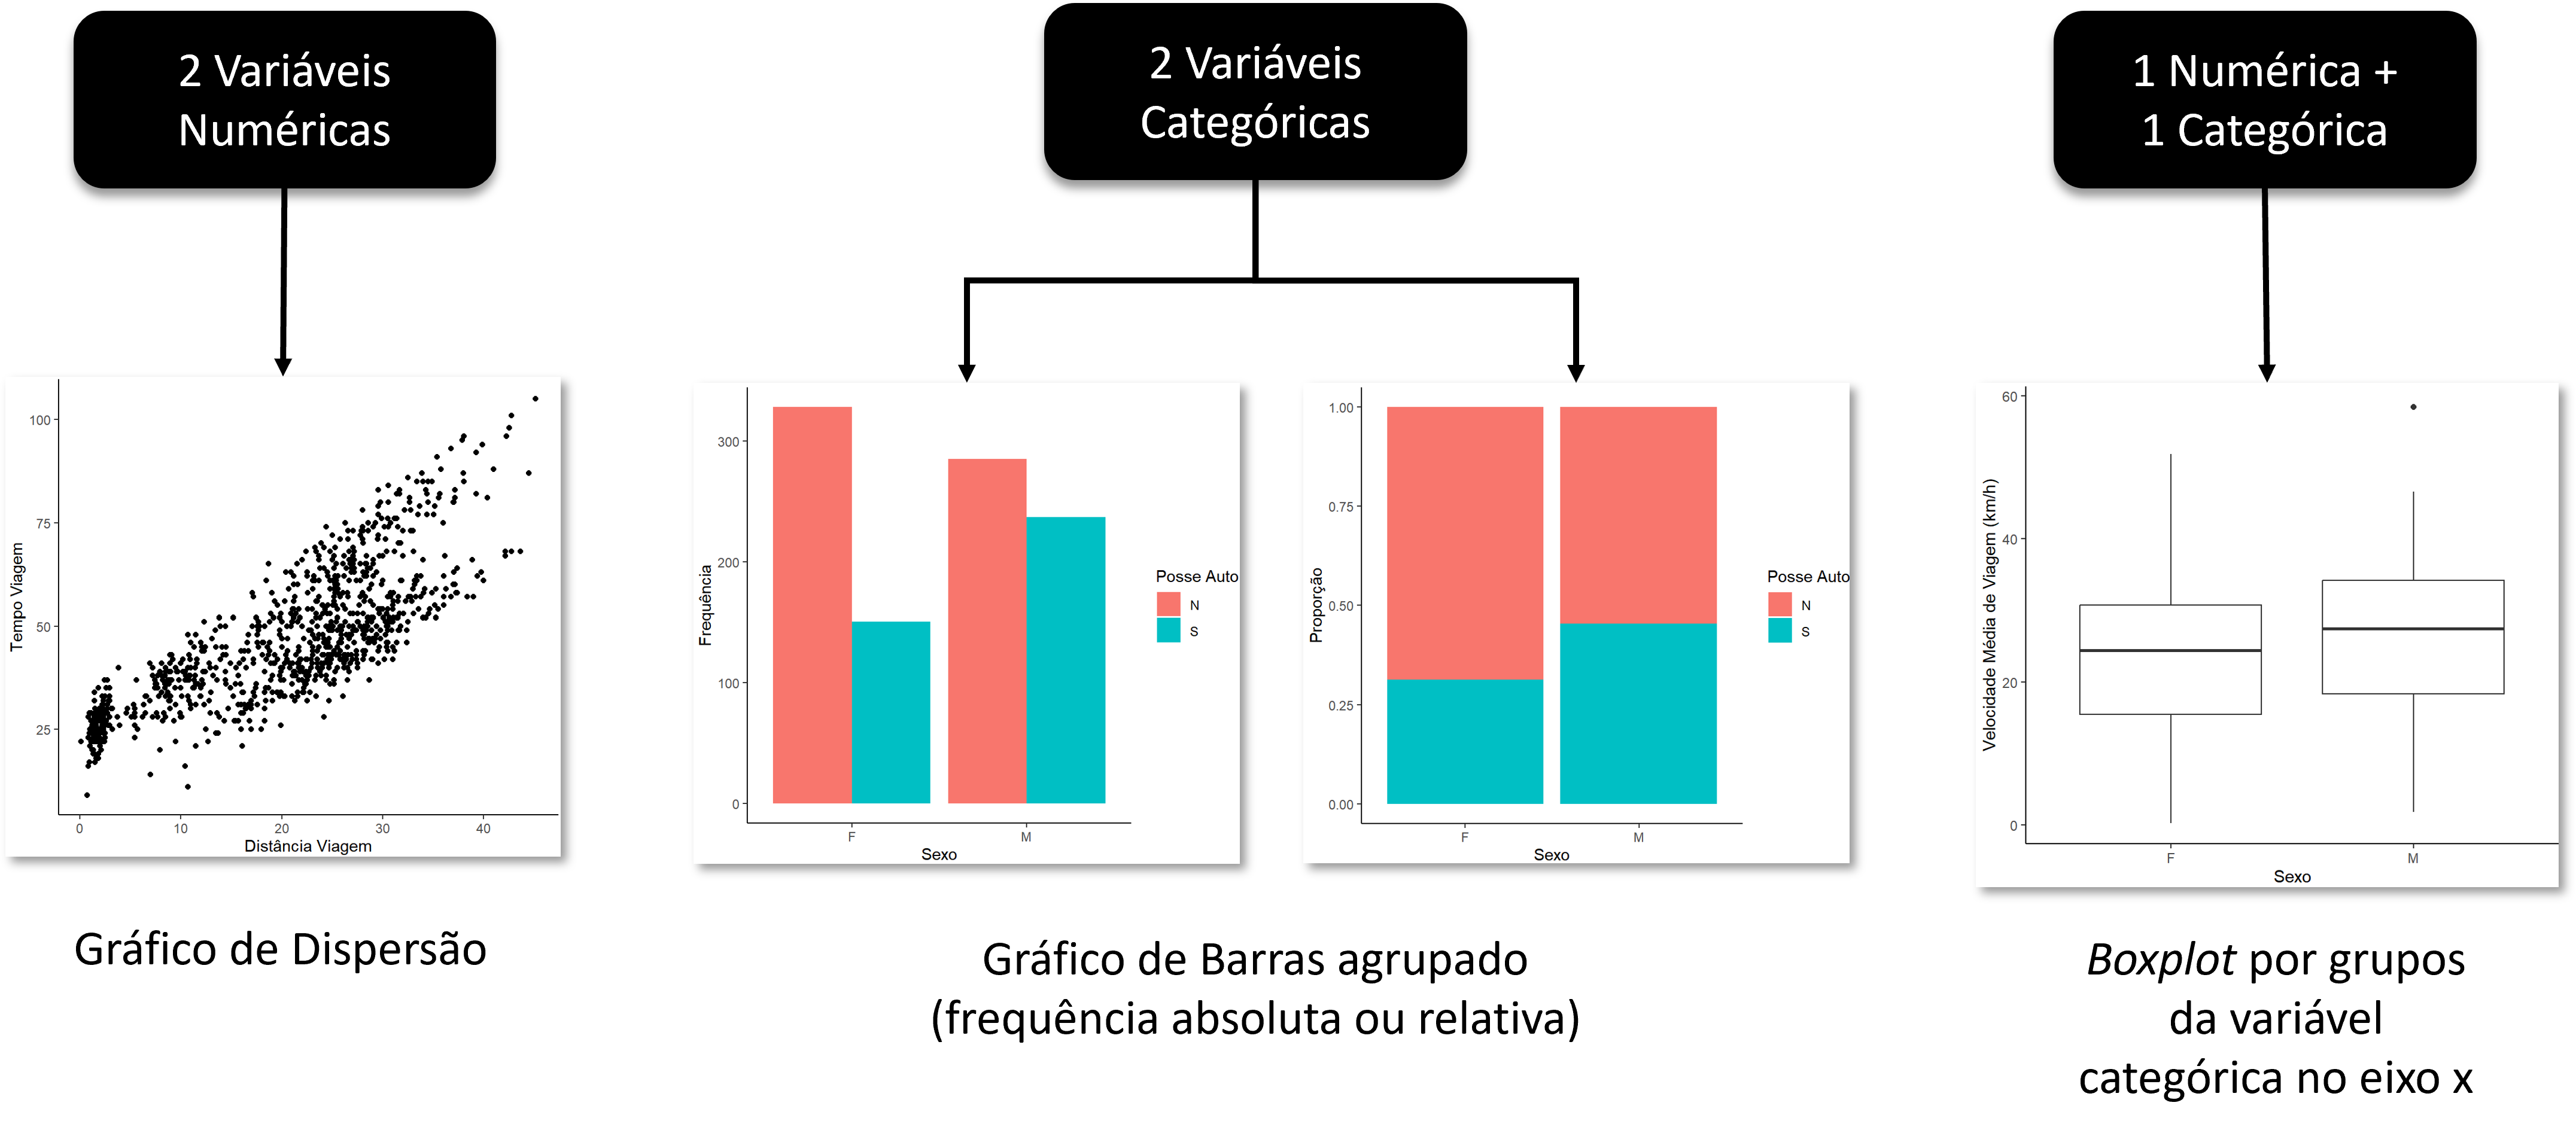
\includegraphics[keepaspectratio]{img/4-visualizacao-de-dados-tabulares/4-27-duas_variaveis.png}}

}

\end{figure}%

\subsection{Duas variáveis
numéricas}\label{duas-variuxe1veis-numuxe9ricas}

O gráfico de dispersão representa cada observação por um ponto cujas
coordenadas são os valores das duas variáveis nos eixos \(x\) e \(y\). É
a representação que melhor aproveita a hierarquia de percepção, porque
usa posição nos dois eixos. Abaixo utilizaremos a camada de geometria
\texttt{geom\_point()} para tanto, indicando dentro do mapeamento
estético, em \texttt{aes()}, quais variáveis da tabela \texttt{em} devem
vir em cada eixo. Neste caso, trabalharemos com distância e tempo de
viagem:

\begin{Shaded}
\begin{Highlighting}[]
\NormalTok{em }\SpecialCharTok{|\textgreater{}}
  \FunctionTok{ggplot}\NormalTok{(}\FunctionTok{aes}\NormalTok{(}\AttributeTok{x =}\NormalTok{ dist\_viagem, }\AttributeTok{y =}\NormalTok{ tempo\_viagem)) }\SpecialCharTok{+}
  \FunctionTok{geom\_point}\NormalTok{() }\SpecialCharTok{+}
  \FunctionTok{labs}\NormalTok{(}\AttributeTok{x =} \StringTok{"Distância da viagem (km)"}\NormalTok{, }\AttributeTok{y =} \StringTok{"Tempo de viagem (h)"}\NormalTok{) }\SpecialCharTok{+}
  \FunctionTok{theme\_bw}\NormalTok{()}
\end{Highlighting}
\end{Shaded}

\begin{figure}[H]

\caption{\label{fig-dispersao}Relação entre distância e tempo de
viagem.}

\centering{

\pandocbounded{
\includegraphics[keepaspectratio]{4-visualizacao-de-dados-tabulares_files/figure-pdf/fig-dispersao-1.pdf}}

}

\end{figure}%

Com muitas observações, muitos pontos se sobrepõem e a densidade da
nuvem fica difícil de avaliar. O argumento \texttt{alpha} resolve o
problema, porque regiões com mais sobreposição ficam visivelmente mais
escuras. Observe que alteramos também o tamanho dos pontos com
\texttt{size}, além da sua coloração com \texttt{color}:

\begin{Shaded}
\begin{Highlighting}[]
\NormalTok{em }\SpecialCharTok{|\textgreater{}}
  \FunctionTok{ggplot}\NormalTok{(}\FunctionTok{aes}\NormalTok{(}\AttributeTok{x =}\NormalTok{ dist\_viagem, }\AttributeTok{y =}\NormalTok{ tempo\_viagem)) }\SpecialCharTok{+}
  \FunctionTok{geom\_point}\NormalTok{(}\AttributeTok{size =} \DecValTok{3}\NormalTok{, }\AttributeTok{alpha =} \FloatTok{0.2}\NormalTok{, }\AttributeTok{color =} \StringTok{"blue"}\NormalTok{) }\SpecialCharTok{+}
  \FunctionTok{labs}\NormalTok{(}
    \AttributeTok{x =} \StringTok{"Distância da viagem (km)"}\NormalTok{,}
    \AttributeTok{y =} \StringTok{"Tempo de viagem (h)"}\NormalTok{,}
    \AttributeTok{title =} \StringTok{"Tempo de viagem em função da distância"}
\NormalTok{  ) }\SpecialCharTok{+}
  \FunctionTok{theme\_bw}\NormalTok{()}
\end{Highlighting}
\end{Shaded}

\begin{figure}[H]

\caption{\label{fig-dispersao-alpha}Relação entre distância e tempo de
viagem com transparência nos pontos.}

\centering{

\pandocbounded{
\includegraphics[keepaspectratio]{4-visualizacao-de-dados-tabulares_files/figure-pdf/fig-dispersao-alpha-1.pdf}}

}

\end{figure}%

A nuvem revela uma relação positiva entre as duas variáveis, com
dispersão crescente à medida que a distância aumenta.

\subsection{Duas variáveis
categóricas}\label{duas-variuxe1veis-categuxf3ricas}

Para cruzar duas variáveis categóricas, uma solução interessante é
mantermos a primeira no eixo horizontal e mapearmos a segunda com o
preenchimento de cor (\texttt{fill}) das barras. Vamos cruzar o sexo do
entrevistado com a posse de automóvel:

\begin{Shaded}
\begin{Highlighting}[]
\NormalTok{em }\SpecialCharTok{|\textgreater{}}
  \FunctionTok{ggplot}\NormalTok{(}\FunctionTok{aes}\NormalTok{(}\AttributeTok{x =}\NormalTok{ sexo, }\AttributeTok{fill =}\NormalTok{ posse\_auto)) }\SpecialCharTok{+}
  \FunctionTok{geom\_bar}\NormalTok{() }\SpecialCharTok{+}
  \FunctionTok{labs}\NormalTok{(}\AttributeTok{x =} \StringTok{"Sexo"}\NormalTok{, }\AttributeTok{y =} \StringTok{"Frequência"}\NormalTok{, }\AttributeTok{fill =} \StringTok{"Possui auto"}\NormalTok{) }\SpecialCharTok{+}
  \FunctionTok{theme\_bw}\NormalTok{()}
\end{Highlighting}
\end{Shaded}

\begin{figure}[H]

\caption{\label{fig-barras-empilhadas}Posse de automóvel por sexo, em
barras empilhadas.}

\centering{

\pandocbounded{
\includegraphics[keepaspectratio]{4-visualizacao-de-dados-tabulares_files/figure-pdf/fig-barras-empilhadas-1.pdf}}

}

\end{figure}%

O comportamento padrão do \texttt{geom\_bar()} é
\texttt{position\ =\ "stack"}, que empilha as categorias. O empilhamento
facilita a leitura do total de cada barra e dificulta a comparação entre
as categorias empilhadas, já que apenas o segmento da base fica alinhado
a uma escala comum. Alterando para \texttt{position\ =\ "dodge"}, as
barras ficam lado a lado e passam a compartilhar a mesma linha de base:

\begin{Shaded}
\begin{Highlighting}[]
\NormalTok{em }\SpecialCharTok{|\textgreater{}}
  \FunctionTok{ggplot}\NormalTok{(}\FunctionTok{aes}\NormalTok{(}\AttributeTok{x =}\NormalTok{ sexo, }\AttributeTok{fill =}\NormalTok{ posse\_auto)) }\SpecialCharTok{+}
  \FunctionTok{geom\_bar}\NormalTok{(}\AttributeTok{position =} \StringTok{"dodge"}\NormalTok{) }\SpecialCharTok{+}
  \FunctionTok{labs}\NormalTok{(}\AttributeTok{x =} \StringTok{"Sexo"}\NormalTok{, }\AttributeTok{y =} \StringTok{"Frequência"}\NormalTok{, }\AttributeTok{fill =} \StringTok{"Possui auto"}\NormalTok{) }\SpecialCharTok{+}
  \FunctionTok{theme\_bw}\NormalTok{()}
\end{Highlighting}
\end{Shaded}

\begin{figure}[H]

\caption{\label{fig-barras-dodge}Posse de automóvel por sexo, em barras
lado a lado.}

\centering{

\pandocbounded{
\includegraphics[keepaspectratio]{4-visualizacao-de-dados-tabulares_files/figure-pdf/fig-barras-dodge-1.pdf}}

}

\end{figure}%

Frequentemente interessa mais a frequência relativa que a absoluta,
sobretudo quando os grupos têm tamanhos diferentes. Aqui existe uma
armadilha comum. Ao calcular a proporção logo após o \texttt{count()},
obtemos a participação de cada combinação no total geral:

\begin{Shaded}
\begin{Highlighting}[]
\NormalTok{em }\SpecialCharTok{|\textgreater{}}
  \FunctionTok{count}\NormalTok{(sexo, posse\_auto) }\SpecialCharTok{|\textgreater{}}
  \FunctionTok{mutate}\NormalTok{(}\AttributeTok{p =}\NormalTok{ n }\SpecialCharTok{/} \FunctionTok{sum}\NormalTok{(n))}
\end{Highlighting}
\end{Shaded}

\begin{verbatim}
# A tibble: 4 x 4
  sexo  posse_auto     n     p
  <fct> <fct>      <int> <dbl>
1 F     N            328 0.328
2 F     S            150 0.15 
3 M     N            285 0.285
4 M     S            237 0.237
\end{verbatim}

As quatro proporções somam 1, e não é isso que queremos. A pergunta
correta é qual a proporção de cada categoria de posse de automóvel
\textbf{dentro} de cada sexo, o que exige agrupar pela primeira variável
antes de calcular:

\begin{Shaded}
\begin{Highlighting}[]
\NormalTok{tab\_sexo\_auto }\OtherTok{\textless{}{-}}\NormalTok{ em }\SpecialCharTok{|\textgreater{}}
  \FunctionTok{group\_by}\NormalTok{(sexo,posse\_auto) }\SpecialCharTok{|\textgreater{}}
  \FunctionTok{summarize}\NormalTok{(}\AttributeTok{n =} \FunctionTok{n}\NormalTok{()) }\SpecialCharTok{|\textgreater{}}
  \FunctionTok{mutate}\NormalTok{(}\AttributeTok{p =}\NormalTok{ n }\SpecialCharTok{/} \FunctionTok{sum}\NormalTok{(n))}
\end{Highlighting}
\end{Shaded}

\begin{verbatim}
`summarise()` has regrouped the output.
i Summaries were computed grouped by sexo and posse_auto.
i Output is grouped by sexo.
i Use `summarise(.groups = "drop_last")` to silence this message.
i Use `summarise(.by = c(sexo, posse_auto))` for per-operation grouping
  (`?dplyr::dplyr_by`) instead.
\end{verbatim}

\begin{Shaded}
\begin{Highlighting}[]
\NormalTok{tab\_sexo\_auto}
\end{Highlighting}
\end{Shaded}

\begin{verbatim}
# A tibble: 4 x 4
# Groups:   sexo [2]
  sexo  posse_auto     n     p
  <fct> <fct>      <int> <dbl>
1 F     N            328 0.686
2 F     S            150 0.314
3 M     N            285 0.546
4 M     S            237 0.454
\end{verbatim}

Outra opção mais enxuta é utilizar \texttt{count()} para ambas as
variáveis primeiro e depois agrupar por sexo e produzir as proporções,
conforme o código abaixo:

\begin{Shaded}
\begin{Highlighting}[]
\NormalTok{tab\_sexo\_auto }\OtherTok{\textless{}{-}}\NormalTok{ em }\SpecialCharTok{|\textgreater{}}
  \FunctionTok{count}\NormalTok{(sexo,posse\_auto) }\SpecialCharTok{|\textgreater{}} 
  \FunctionTok{group\_by}\NormalTok{(sexo) }\SpecialCharTok{|\textgreater{}}
  \FunctionTok{mutate}\NormalTok{(}\AttributeTok{p =}\NormalTok{ n }\SpecialCharTok{/} \FunctionTok{sum}\NormalTok{(n))}

\NormalTok{tab\_sexo\_auto}
\end{Highlighting}
\end{Shaded}

\begin{verbatim}
# A tibble: 4 x 4
# Groups:   sexo [2]
  sexo  posse_auto     n     p
  <fct> <fct>      <int> <dbl>
1 F     N            328 0.686
2 F     S            150 0.314
3 M     N            285 0.546
4 M     S            237 0.454
\end{verbatim}

Observe que em ambos os casos as proporções somam 1 dentro de cada sexo,
e o gráfico empilhado passa a comparar composições. Note também como é
possível agora afirmar que há indícios de associação entre as variáveis
sexo e automóvel, já que os dados apontam uma maior posse de automóvel
entre pessoas do sexo masculino, algo que não era imediatamente
identificável nos gráficos de barra com valores absolutos.

\begin{Shaded}
\begin{Highlighting}[]
\NormalTok{tab\_sexo\_auto }\SpecialCharTok{|\textgreater{}}
  \FunctionTok{ggplot}\NormalTok{(}\FunctionTok{aes}\NormalTok{(}\AttributeTok{x =}\NormalTok{ sexo, }\AttributeTok{y =}\NormalTok{ p, }\AttributeTok{fill =}\NormalTok{ posse\_auto)) }\SpecialCharTok{+}
  \FunctionTok{geom\_col}\NormalTok{() }\SpecialCharTok{+}
  \FunctionTok{labs}\NormalTok{(}\AttributeTok{x =} \StringTok{"Sexo"}\NormalTok{,  }\AttributeTok{y =} \StringTok{"Proporção"}\NormalTok{, }\AttributeTok{fill =} \StringTok{"Possui auto"}\NormalTok{) }\SpecialCharTok{+}
  \FunctionTok{theme\_bw}\NormalTok{()}
\end{Highlighting}
\end{Shaded}

\begin{figure}[H]

\caption{\label{fig-barras-relativa}Composição da posse de automóvel
dentro de cada sexo.}

\centering{

\pandocbounded{
\includegraphics[keepaspectratio]{4-visualizacao-de-dados-tabulares_files/figure-pdf/fig-barras-relativa-1.pdf}}

}

\end{figure}%

\subsection{Uma variável numérica e outra
categórica}\label{uma-variuxe1vel-numuxe9rica-e-outra-categuxf3rica}

Quando cruzamos uma variável numérica com uma categórica, o objetivo
costuma ser comparar a distribuição da primeira entre os níveis da
segunda. O boxplot é a opção mais econômica, porque coloca vários
resumos lado a lado com os eixos alinhados:

\begin{Shaded}
\begin{Highlighting}[]
\NormalTok{em }\SpecialCharTok{|\textgreater{}}
  \FunctionTok{ggplot}\NormalTok{(}\FunctionTok{aes}\NormalTok{(}\AttributeTok{x =}\NormalTok{ modo\_viagem, }\AttributeTok{y =}\NormalTok{ vel\_media\_viagem)) }\SpecialCharTok{+}
  \FunctionTok{geom\_boxplot}\NormalTok{() }\SpecialCharTok{+}
  \FunctionTok{labs}\NormalTok{(}\AttributeTok{x =} \StringTok{"Modo de viagem"}\NormalTok{, }\AttributeTok{y =} \StringTok{"Velocidade média (km/h)"}\NormalTok{) }\SpecialCharTok{+}
  \FunctionTok{theme\_bw}\NormalTok{()}
\end{Highlighting}
\end{Shaded}

\begin{figure}[H]

\caption{\label{fig-boxplot-grupos}Velocidade média da viagem por modo
de transporte.}

\centering{

\pandocbounded{
\includegraphics[keepaspectratio]{4-visualizacao-de-dados-tabulares_files/figure-pdf/fig-boxplot-grupos-1.pdf}}

}

\end{figure}%

O gráfico separa nitidamente os modos motorizados dos não motorizados, e
mostra também que a dispersão interna varia bastante de um modo para
outro. Note que diferente do caso do \emph{boxplot} para uma única
variável numérica, agora o eixo \(x\) faz sentido e representa de forma
categorizada os níveis da variável modo de viagem.

Uma alternativa é manter o histograma e usar a variável categórica para
subdividir o gráfico em painéis, o que introduz a camada de
\textbf{facetas}. A função \texttt{facet\_grid()} recebe uma fórmula com
dois lados separados pelo til (\texttt{\textasciitilde{}}). A variável
escrita antes do til define as linhas da grade de painéis e a variável
escrita depois dele define as colunas. Quando um dos lados não recebe
variável alguma, colocamos um ponto (\texttt{.}) no lugar, que funciona
como marcador de ausência. A fórmula \texttt{sexo\ \textasciitilde{}\ .}
pede, portanto, uma grade com uma linha para cada sexo e nenhuma divisão
em colunas, o que empilha os painéis verticalmente\footnote{Caso
  quiséssemos que a subdivisão fosse por coluna, faríamos
  \texttt{.\ \textasciitilde{}\ \ sexo}, o que empilharia os paines
  horizontalmente}:

\begin{Shaded}
\begin{Highlighting}[]
\NormalTok{em }\SpecialCharTok{|\textgreater{}}
  \FunctionTok{ggplot}\NormalTok{(}\FunctionTok{aes}\NormalTok{(}\AttributeTok{x =}\NormalTok{ vel\_media\_viagem)) }\SpecialCharTok{+}
  \FunctionTok{geom\_histogram}\NormalTok{(}\AttributeTok{color =} \StringTok{"black"}\NormalTok{, }\AttributeTok{fill =} \StringTok{"gray70"}\NormalTok{) }\SpecialCharTok{+}
  \FunctionTok{facet\_grid}\NormalTok{(sexo }\SpecialCharTok{\textasciitilde{}}\NormalTok{ .) }\SpecialCharTok{+}
  \FunctionTok{labs}\NormalTok{(}\AttributeTok{x =} \StringTok{"Velocidade média (km/h)"}\NormalTok{, }\AttributeTok{y =} \StringTok{"Frequência"}\NormalTok{) }\SpecialCharTok{+}
  \FunctionTok{theme\_bw}\NormalTok{()}
\end{Highlighting}
\end{Shaded}

\begin{figure}[H]

\caption{\label{fig-hist-facet}Distribuição da velocidade média por
sexo, em painéis.}

\centering{

\pandocbounded{
\includegraphics[keepaspectratio]{4-visualizacao-de-dados-tabulares_files/figure-pdf/fig-hist-facet-1.pdf}}

}

\end{figure}%

Uma terceira alternativa substitui as barras por curvas de densidade
sobrepostas através da camada de geometria \texttt{geom\_density()}, o
que facilita a comparação direta das formas por eliminar a separação em
painéis:

\begin{Shaded}
\begin{Highlighting}[]
\NormalTok{em }\SpecialCharTok{|\textgreater{}}
  \FunctionTok{ggplot}\NormalTok{(}\FunctionTok{aes}\NormalTok{(}\AttributeTok{x =}\NormalTok{ vel\_media\_viagem, }\AttributeTok{fill =}\NormalTok{ sexo)) }\SpecialCharTok{+}
  \FunctionTok{geom\_density}\NormalTok{(}\AttributeTok{alpha =} \FloatTok{0.5}\NormalTok{) }\SpecialCharTok{+}
  \FunctionTok{labs}\NormalTok{(}\AttributeTok{x =} \StringTok{"Velocidade média (km/h)"}\NormalTok{, }\AttributeTok{y =} \StringTok{"Densidade"}\NormalTok{, }\AttributeTok{fill =} \StringTok{"Sexo"}\NormalTok{) }\SpecialCharTok{+}
  \FunctionTok{theme\_bw}\NormalTok{()}
\end{Highlighting}
\end{Shaded}

\begin{figure}[H]

\caption{\label{fig-densidade}Densidade da velocidade média por sexo,
com curvas sobrepostas.}

\centering{

\pandocbounded{
\includegraphics[keepaspectratio]{4-visualizacao-de-dados-tabulares_files/figure-pdf/fig-densidade-1.pdf}}

}

\end{figure}%

Vale entender de onde vem essa curva, porque ela não é simplesmente o
contorno das barras de um histograma. Em vez de contar quantas
observações caem dentro de cada intervalo, o R substitui cada observação
por uma pequena curva em forma de sino, centrada no valor observado, e
soma todas essas curvas ao longo do eixo horizontal. Onde as observações
estão próximas umas das outras, as curvas se sobrepõem e a soma assume
valores altos. Onde há poucas observações, a soma permanece baixa. O
resultado é um perfil contínuo da distribuição, sem os degraus do
histograma\footnote{O procedimento se chama \emph{estimação de densidade
  por kernel}, e cada uma dessas pequenas curvas é o \emph{kernel} que
  dá nome ao método. A largura dessas curvas controla a suavidade do
  resultado, do mesmo modo que a largura das barras controla a aparência
  do histograma. Curvas estreitas produzem um traçado cheio de
  ondulações que refletem particularidades da amostra, e curvas largas
  produzem um traçado liso demais, a ponto de esconder características
  reais da distribuição. O R escolhe sozinho uma largura razoável a
  partir do tamanho da amostra e da dispersão dos dados, e o argumento
  \texttt{adjust} permite pedir mais suavização, com valores acima de 1,
  ou menos suavização, com valores abaixo de 1.}.

\section{Visualizando três ou mais
variáveis}\label{visualizando-truxeas-ou-mais-variuxe1veis}

A partir da terceira variável, todas as representações consistem em
acrescentar camadas de codificação aos gráficos que já conhecemos. É
aqui que a hierarquia de percepção se torna um critério prático de
decisão (Figura~\ref{fig-hierarquia-percepcao}), porque precisamos
distribuir as variáveis entre elementos visuais de eficácia desigual. A
regra de bolso é reservar os eixos com adequada alocação de facetas, que
ocupam o topo da hierarquia, para as variáveis mais importantes da
análise, e alocar as demais a cor, tamanho ou forma.

\subsection{Três e quatro variáveis
numéricas}\label{truxeas-e-quatro-variuxe1veis-numuxe9ricas}

Partindo do gráfico de dispersão, a terceira variável numérica pode ser
mapeada ao tamanho dos pontos. No caso abaixo, inserimos a variável
\texttt{idade} no mapeamento estético a ser representada pelo tamanho
desse ponto.

\begin{Shaded}
\begin{Highlighting}[]
\NormalTok{em }\SpecialCharTok{|\textgreater{}}
  \FunctionTok{ggplot}\NormalTok{(}\FunctionTok{aes}\NormalTok{(}\AttributeTok{x =}\NormalTok{ dist\_viagem, }\AttributeTok{y =}\NormalTok{ tempo\_viagem, }\AttributeTok{size =}\NormalTok{ idade)) }\SpecialCharTok{+}
  \FunctionTok{geom\_point}\NormalTok{(}\AttributeTok{alpha =} \FloatTok{0.3}\NormalTok{) }\SpecialCharTok{+}
  \FunctionTok{labs}\NormalTok{(}\AttributeTok{x =} \StringTok{"Distância da viagem (km)"}\NormalTok{, }\AttributeTok{y =} \StringTok{"Tempo de viagem (h)"}\NormalTok{, }\AttributeTok{size =} \StringTok{"Idade"}\NormalTok{) }\SpecialCharTok{+}
  \FunctionTok{theme\_bw}\NormalTok{()}
\end{Highlighting}
\end{Shaded}

\begin{figure}[H]

\caption{\label{fig-3num-size}Tempo e distância de viagem com a idade
representada pelo tamanho dos pontos.}

\centering{

\pandocbounded{
\includegraphics[keepaspectratio]{4-visualizacao-de-dados-tabulares_files/figure-pdf/fig-3num-size-1.pdf}}

}

\end{figure}%

Cabe uma explicação sobre o que o R faz com os valores de idade ao
desenhar os pontos. O que ele varia não é o diâmetro do círculo, e sim a
sua área, o que na prática significa extrair a raiz quadrada do valor
antes de definir o raio de cada ponto. Conforme já vimos, a razão é
perceptiva, pois quando comparamos círculos, julgamos a mancha que cada
um ocupa na tela, de modo que dobrar o diâmetro quadruplica a área e faz
o ponto parecer muito maior do que a diferença nos dados justifica. Ao
trabalhar com a área, o \texttt{ggplot2} mantém a impressão visual mais
próxima da variação real da variável\footnote{Por padrão, os pontos
  ficam entre 1 e 6 milímetros, com o menor valor observado recebendo o
  menor tamanho e o maior valor recebendo o maior. O tamanho comunica,
  portanto, a posição relativa de cada observação dentro da faixa
  observada, e não uma proporção exata, de forma que um ponto com o
  dobro da área não corresponde a alguém com o dobro da idade.}.

Alternativamente, a terceira variável pode ser mapeada à intensidade de
cor, conforme o gráfico abaixo. Note que o elemento visual
(Figura~\ref{fig-elementos-visuais}) utilizado a partir do mapeamento
estético do \texttt{color} é a \emph{saturação} e não a \emph{matiz}.

\begin{Shaded}
\begin{Highlighting}[]
\NormalTok{em }\SpecialCharTok{|\textgreater{}}
  \FunctionTok{ggplot}\NormalTok{(}\FunctionTok{aes}\NormalTok{(}\AttributeTok{x =}\NormalTok{ dist\_viagem, }\AttributeTok{y =}\NormalTok{ tempo\_viagem, }\AttributeTok{color =}\NormalTok{ idade)) }\SpecialCharTok{+}
  \FunctionTok{geom\_point}\NormalTok{() }\SpecialCharTok{+}
  \FunctionTok{labs}\NormalTok{(}\AttributeTok{x =} \StringTok{"Distância da viagem (km)"}\NormalTok{, }\AttributeTok{y =} \StringTok{"Tempo de viagem (h)"}\NormalTok{, }\AttributeTok{color =} \StringTok{"Idade"}\NormalTok{) }\SpecialCharTok{+}
  \FunctionTok{theme\_bw}\NormalTok{()}
\end{Highlighting}
\end{Shaded}

\begin{figure}[H]

\caption{\label{fig-3num-color}Tempo e distância de viagem com a idade
representada pela intensidade de cor.}

\centering{

\pandocbounded{
\includegraphics[keepaspectratio]{4-visualizacao-de-dados-tabulares_files/figure-pdf/fig-3num-color-1.pdf}}

}

\end{figure}%

Combinando os dois recursos, chegamos a quatro variáveis numéricas em um
único gráfico. É interessante apresentar, neste momento, possibilidades
de uso das camadas de \textbf{escalas} da Gramática dos Gráficos
(Figura~\ref{fig-camadas-gg}), onde podemos editar cores, tamanhos e
formatos além da coloração padrão do \texttt{ggplot2}. No caso abaixo,
utilizamos a função \texttt{scale\_color\_distiller()} permite trocar a
paleta de cores por uma sequencial mais legível que a padrão. Para este
gráfico, empregamos a paleta ``BuPu'' que vai do azul claro até o roxo
escuro, garantindo com o \texttt{direction\ =\ 1} que este seja o
sentido do gradiente\footnote{caso queiramos que vá do roxo escuro até o
  azul claro, utilizamos \texttt{direction\ =\ -1}. Por incrível que
  pareça, essa última escoha é o \emph{default} das funções de escala do
  \texttt{ggplot2}, ou seja, se nada for definido para
  \texttt{direction}, a função entenderá que o valor é \texttt{-1}}.

\begin{Shaded}
\begin{Highlighting}[]
\NormalTok{em }\SpecialCharTok{|\textgreater{}}
  \FunctionTok{ggplot}\NormalTok{(}\FunctionTok{aes}\NormalTok{(}\AttributeTok{x =}\NormalTok{ dist\_viagem, }\AttributeTok{y =}\NormalTok{ tempo\_viagem,}
             \AttributeTok{size =}\NormalTok{ renda, }\AttributeTok{color =}\NormalTok{ idade)) }\SpecialCharTok{+}
  \FunctionTok{geom\_point}\NormalTok{(}\AttributeTok{alpha =} \FloatTok{0.6}\NormalTok{) }\SpecialCharTok{+}
  \FunctionTok{scale\_color\_distiller}\NormalTok{(}\AttributeTok{palette =} \StringTok{"BuPu"}\NormalTok{, }\AttributeTok{direction =} \DecValTok{1}\NormalTok{) }\SpecialCharTok{+}
  \FunctionTok{labs}\NormalTok{(}\AttributeTok{x =} \StringTok{"Distância da viagem (km)"}\NormalTok{, }\AttributeTok{y =} \StringTok{"Tempo de viagem (h)"}\NormalTok{,}
       \AttributeTok{size =} \StringTok{"Renda (R$)"}\NormalTok{,}\AttributeTok{color =} \StringTok{"Idade"}\NormalTok{) }\SpecialCharTok{+}
  \FunctionTok{theme\_bw}\NormalTok{()}
\end{Highlighting}
\end{Shaded}

\begin{figure}[H]

\caption{\label{fig-4num}Quatro variáveis numéricas representadas por
posição, tamanho e cor.}

\centering{

\pandocbounded{
\includegraphics[keepaspectratio]{4-visualizacao-de-dados-tabulares_files/figure-pdf/fig-4num-1.pdf}}

}

\end{figure}%

Este é um bom momento para lembrar que a possibilidade técnica não
implica boa prática. \emph{Área} e \emph{saturação} ocupam posições
baixas na hierarquia de percepção, de modo que renda e idade aqui
comunicam tendências gerais e não permitem comparações precisas. Quando
a leitura exata da terceira ou quarta variável for essencial, é
preferível produzir vários gráficos mais simples.

\subsection{Duas numéricas e uma
categórica}\label{duas-numuxe9ricas-e-uma-categuxf3rica}

Para uma variável categórica, o recurso natural é a matiz, que apesar de
contraindicada para representar magnitude, é bastante adequada para
distinguir categorias:

\begin{Shaded}
\begin{Highlighting}[]
\NormalTok{em }\SpecialCharTok{|\textgreater{}}
  \FunctionTok{ggplot}\NormalTok{(}\FunctionTok{aes}\NormalTok{(}\AttributeTok{x =}\NormalTok{ dist\_viagem, }\AttributeTok{y =}\NormalTok{ tempo\_viagem, }\AttributeTok{color =}\NormalTok{ modo\_viagem)) }\SpecialCharTok{+}
  \FunctionTok{geom\_point}\NormalTok{(}\AttributeTok{alpha =} \FloatTok{0.6}\NormalTok{) }\SpecialCharTok{+}
  \FunctionTok{labs}\NormalTok{(}\AttributeTok{x =} \StringTok{"Distância da viagem (km)"}\NormalTok{, }\AttributeTok{y =} \StringTok{"Tempo de viagem (h)"}\NormalTok{,}
       \AttributeTok{color =} \StringTok{"Modo de viagem"}\NormalTok{) }\SpecialCharTok{+}
  \FunctionTok{theme\_bw}\NormalTok{()}
\end{Highlighting}
\end{Shaded}

\begin{figure}[H]

\caption{\label{fig-2num-1cat-cor}Tempo e distância de viagem por modo
de transporte, distinguidos por cor.}

\centering{

\pandocbounded{
\includegraphics[keepaspectratio]{4-visualizacao-de-dados-tabulares_files/figure-pdf/fig-2num-1cat-cor-1.pdf}}

}

\end{figure}%

A separação entre os modos fica evidente, com cada categoria formando
uma nuvem de pontos com faixas destacadas no diagrama distância VS.
viagem. A \emph{forma} dos pontos é outra alternativa para variáveis
categóricas, embora seja menos eficaz que a cor e só funcione bem com
poucos níveis e poucos pontos a serem mostrados. No caso abaixo,
passamos a variável \texttt{sexo} no argumento \texttt{shape} da função
\texttt{aes()} de mapeamento estético:

\begin{Shaded}
\begin{Highlighting}[]
\NormalTok{em }\SpecialCharTok{|\textgreater{}}
  \FunctionTok{ggplot}\NormalTok{(}\FunctionTok{aes}\NormalTok{(}\AttributeTok{x =}\NormalTok{ dist\_viagem, }\AttributeTok{y =}\NormalTok{ tempo\_viagem, }\AttributeTok{shape =}\NormalTok{ sexo)) }\SpecialCharTok{+}
  \FunctionTok{geom\_point}\NormalTok{(}\AttributeTok{alpha =} \FloatTok{0.5}\NormalTok{, }\AttributeTok{size =} \DecValTok{2}\NormalTok{) }\SpecialCharTok{+}
  \FunctionTok{labs}\NormalTok{(}\AttributeTok{x =} \StringTok{"Distância da viagem (km)"}\NormalTok{, }\AttributeTok{y =} \StringTok{"Tempo de viagem (h)"}\NormalTok{, }
       \AttributeTok{shape =} \StringTok{"Sexo"}\NormalTok{) }\SpecialCharTok{+}
  \FunctionTok{theme\_bw}\NormalTok{()}
\end{Highlighting}
\end{Shaded}

\begin{figure}[H]

\caption{\label{fig-2num-1cat-forma}Tempo e distância de viagem por
sexo, distinguidos pela forma dos pontos.}

\centering{

\pandocbounded{
\includegraphics[keepaspectratio]{4-visualizacao-de-dados-tabulares_files/figure-pdf/fig-2num-1cat-forma-1.pdf}}

}

\end{figure}%

\subsection{Duas categóricas e uma
numérica}\label{duas-categuxf3ricas-e-uma-numuxe9rica}

Partindo do \emph{boxplot} agrupado, a segunda variável categórica pode
ser mapeada ao preenchimento das caixas. A função
\texttt{scale\_fill\_manual()} permite definir cores customizadas para
cada nível definido no mapeamento estético de cor de preenchimento
(\texttt{fill}), através do seu argumento \texttt{values}\footnote{Neste
  caso, é importante entender qual a ordem desses níveis preliminarmente
  para saber qual categoria receberá qual cor}:

\begin{Shaded}
\begin{Highlighting}[]
\NormalTok{em }\SpecialCharTok{|\textgreater{}}
  \FunctionTok{ggplot}\NormalTok{(}\FunctionTok{aes}\NormalTok{(}\AttributeTok{x =}\NormalTok{ sexo, }\AttributeTok{y =}\NormalTok{ vel\_media\_viagem, }\AttributeTok{fill =}\NormalTok{ posse\_auto)) }\SpecialCharTok{+}
  \FunctionTok{geom\_boxplot}\NormalTok{() }\SpecialCharTok{+}
  \FunctionTok{scale\_fill\_manual}\NormalTok{(}\AttributeTok{values =} \FunctionTok{c}\NormalTok{(}\StringTok{"\#E4A11B"}\NormalTok{, }\StringTok{"\#3B71CA"}\NormalTok{)) }\SpecialCharTok{+}
  \FunctionTok{labs}\NormalTok{(}\AttributeTok{x =} \StringTok{"Sexo"}\NormalTok{, }\AttributeTok{y =} \StringTok{"Velocidade média (km/h)"}\NormalTok{, }\AttributeTok{fill =} \StringTok{"Possui auto"}\NormalTok{) }\SpecialCharTok{+}
  \FunctionTok{theme\_bw}\NormalTok{()}
\end{Highlighting}
\end{Shaded}

\begin{figure}[H]

\caption{\label{fig-2cat-1num-fill}Velocidade média por sexo e posse de
automóvel, com as caixas distinguidas por cor.}

\centering{

\pandocbounded{
\includegraphics[keepaspectratio]{4-visualizacao-de-dados-tabulares_files/figure-pdf/fig-2cat-1num-fill-1.pdf}}

}

\end{figure}%

Ou então às facetas, o que separa os grupos em painéis distintos:

\begin{Shaded}
\begin{Highlighting}[]
\NormalTok{em }\SpecialCharTok{|\textgreater{}}
  \FunctionTok{ggplot}\NormalTok{(}\FunctionTok{aes}\NormalTok{(}\AttributeTok{x =}\NormalTok{ sexo, }\AttributeTok{y =}\NormalTok{ vel\_media\_viagem)) }\SpecialCharTok{+}
  \FunctionTok{geom\_boxplot}\NormalTok{() }\SpecialCharTok{+}
  \FunctionTok{facet\_grid}\NormalTok{(. }\SpecialCharTok{\textasciitilde{}}\NormalTok{ posse\_auto) }\SpecialCharTok{+}
  \FunctionTok{labs}\NormalTok{(}\AttributeTok{x =} \StringTok{"Sexo"}\NormalTok{, }\AttributeTok{y =} \StringTok{"Velocidade média (km/h)"}\NormalTok{) }\SpecialCharTok{+}
  \FunctionTok{theme\_bw}\NormalTok{()}
\end{Highlighting}
\end{Shaded}

\begin{figure}[H]

\caption{\label{fig-2cat-1num-facet}Velocidade média por sexo, em
painéis definidos pela posse de automóvel.}

\centering{

\pandocbounded{
\includegraphics[keepaspectratio]{4-visualizacao-de-dados-tabulares_files/figure-pdf/fig-2cat-1num-facet-1.pdf}}

}

\end{figure}%

A escolha entre as duas depende da comparação que interessa. Com cor,
comparamos os níveis da segunda categórica dentro de cada nível da
primeira, porque as caixas ficam próximas. Com facetas, comparamos o
padrão geral entre os painéis.

\subsection{Três e quatro variáveis
categóricas}\label{truxeas-e-quatro-variuxe1veis-categuxf3ricas}

Com três variáveis categóricas e nenhuma numérica, o que resta a
representar é a contagem de observações. Combinamos então eixo
horizontal, preenchimento e facetas, uma para cada variável, mantendo a
contagem no eixo vertical. No caso abaixo, os paineis serão formados por
cada modo de viagem, junto com o sexo no eixo \(x\) e a posse de
automóvel como cor de preenchimento:

\begin{Shaded}
\begin{Highlighting}[]
\NormalTok{em }\SpecialCharTok{|\textgreater{}}
  \FunctionTok{count}\NormalTok{(sexo, posse\_auto, modo\_viagem) }\SpecialCharTok{|\textgreater{}}
  \FunctionTok{ggplot}\NormalTok{(}\FunctionTok{aes}\NormalTok{(}\AttributeTok{x =}\NormalTok{ sexo, }\AttributeTok{y =}\NormalTok{ n, }\AttributeTok{fill =}\NormalTok{ posse\_auto)) }\SpecialCharTok{+}
  \FunctionTok{geom\_col}\NormalTok{(}\AttributeTok{position =} \StringTok{"dodge"}\NormalTok{) }\SpecialCharTok{+}
  \FunctionTok{facet\_grid}\NormalTok{(. }\SpecialCharTok{\textasciitilde{}}\NormalTok{ modo\_viagem) }\SpecialCharTok{+}
  \FunctionTok{labs}\NormalTok{(}\AttributeTok{x =} \StringTok{"Sexo"}\NormalTok{,  }\AttributeTok{y =} \StringTok{"Frequência"}\NormalTok{, }\AttributeTok{fill =} \StringTok{"Possui auto"}\NormalTok{) }\SpecialCharTok{+}
  \FunctionTok{theme\_bw}\NormalTok{()}
\end{Highlighting}
\end{Shaded}

\begin{figure}[H]

\caption{\label{fig-3cat-abs}Frequência absoluta por sexo, posse de
automóvel e modo de viagem.}

\centering{

\pandocbounded{
\includegraphics[keepaspectratio]{4-visualizacao-de-dados-tabulares_files/figure-pdf/fig-3cat-abs-1.pdf}}

}

\end{figure}%

A versão em frequência relativa exige o mesmo cuidado com o agrupamento
visto anteriormente. É preciso, de antemão, entender como o gráfico será
estruturado, mais especificamente onde as variáveis serão relativizadas.
Para que cada barra empilhada represente a composição de posse de
automóvel dentro de uma combinação de sexo e modo de viagem, agrupamos
por essas duas últimas variáveis antes de calcular a proporção. Veja
primeiramente a tabela sumarizada:

\begin{Shaded}
\begin{Highlighting}[]
\NormalTok{em }\SpecialCharTok{|\textgreater{}}
  \FunctionTok{count}\NormalTok{(sexo, modo\_viagem, posse\_auto) }\SpecialCharTok{|\textgreater{}}
  \FunctionTok{group\_by}\NormalTok{(sexo, modo\_viagem) }\SpecialCharTok{|\textgreater{}}
  \FunctionTok{mutate}\NormalTok{(}\AttributeTok{p =}\NormalTok{ n }\SpecialCharTok{/} \FunctionTok{sum}\NormalTok{(n))}
\end{Highlighting}
\end{Shaded}

\begin{verbatim}
# A tibble: 16 x 5
# Groups:   sexo, modo_viagem [8]
   sexo  modo_viagem  posse_auto     n     p
   <fct> <fct>        <fct>      <int> <dbl>
 1 F     A pé         N             56 0.659
 2 F     A pé         S             29 0.341
 3 F     Bicicleta    N             44 0.721
 4 F     Bicicleta    S             17 0.279
 5 F     Carro ou App N             66 0.471
 6 F     Carro ou App S             74 0.529
 7 F     TP           N            162 0.844
 8 F     TP           S             30 0.156
 9 M     A pé         N             45 0.692
10 M     A pé         S             20 0.308
11 M     Bicicleta    N             46 0.575
12 M     Bicicleta    S             34 0.425
13 M     Carro ou App N             87 0.362
14 M     Carro ou App S            153 0.638
15 M     TP           N            107 0.781
16 M     TP           S             30 0.219
\end{verbatim}

Note como as proporções de sem (N) e com (S) automóvel agora somam 1
(100\%) em cada combinação de categorias de sexo e modo de viagem. Na
sequência, produzimos o gráfico de barras em frequência relativa a
partir dessa tabela:

\begin{Shaded}
\begin{Highlighting}[]
\NormalTok{em }\SpecialCharTok{|\textgreater{}}
  \FunctionTok{count}\NormalTok{(sexo, modo\_viagem, posse\_auto) }\SpecialCharTok{|\textgreater{}}
  \FunctionTok{group\_by}\NormalTok{(sexo, modo\_viagem) }\SpecialCharTok{|\textgreater{}}
  \FunctionTok{mutate}\NormalTok{(}\AttributeTok{p =}\NormalTok{ n }\SpecialCharTok{/} \FunctionTok{sum}\NormalTok{(n)) }\SpecialCharTok{|\textgreater{}}
  \FunctionTok{ggplot}\NormalTok{(}\FunctionTok{aes}\NormalTok{(}\AttributeTok{x =}\NormalTok{ sexo, }\AttributeTok{y =}\NormalTok{ p, }\AttributeTok{fill =}\NormalTok{ posse\_auto)) }\SpecialCharTok{+}
  \FunctionTok{geom\_col}\NormalTok{() }\SpecialCharTok{+}
  \FunctionTok{facet\_grid}\NormalTok{(. }\SpecialCharTok{\textasciitilde{}}\NormalTok{ modo\_viagem) }\SpecialCharTok{+}
  \FunctionTok{labs}\NormalTok{(}\AttributeTok{x =} \StringTok{"Sexo"}\NormalTok{, }\AttributeTok{y =} \StringTok{"Proporção"}\NormalTok{, }\AttributeTok{fill =} \StringTok{"Possui auto"}\NormalTok{) }\SpecialCharTok{+}
  \FunctionTok{theme\_bw}\NormalTok{()}
\end{Highlighting}
\end{Shaded}

\begin{figure}[H]

\caption{\label{fig-3cat-rel}Composição da posse de automóvel por sexo e
modo de viagem.}

\centering{

\pandocbounded{
\includegraphics[keepaspectratio]{4-visualizacao-de-dados-tabulares_files/figure-pdf/fig-3cat-rel-1.pdf}}

}

\end{figure}%

Uma quarta variável categórica cabe ainda na segunda dimensão do grid de
painéis. Vamos criar uma variável dicotômica de faixa etária e usá-la
nas linhas do grid, deixando o modo de viagem nas colunas, e produzir
mais um gráfico com frequência relativa, agrupando a posse de automóvel
agora pelas variáveis sexo, posse de automóvel e faixa etária:

\begin{Shaded}
\begin{Highlighting}[]
\NormalTok{em }\SpecialCharTok{|\textgreater{}}
  \FunctionTok{mutate}\NormalTok{(}\AttributeTok{faixa\_etaria =} \FunctionTok{ifelse}\NormalTok{(idade }\SpecialCharTok{\textgreater{}} \DecValTok{40}\NormalTok{, }\StringTok{"Mais de 40 anos"}\NormalTok{, }\StringTok{"Até 40 anos"}\NormalTok{)) }\SpecialCharTok{|\textgreater{}}
  \FunctionTok{count}\NormalTok{(sexo, modo\_viagem, faixa\_etaria, posse\_auto) }\SpecialCharTok{|\textgreater{}}
  \FunctionTok{group\_by}\NormalTok{(sexo, faixa\_etaria, modo\_viagem) }\SpecialCharTok{|\textgreater{}} 
  \FunctionTok{mutate}\NormalTok{(}\AttributeTok{p =}\NormalTok{ n }\SpecialCharTok{/} \FunctionTok{sum}\NormalTok{(n)) }\SpecialCharTok{|\textgreater{}}
  \FunctionTok{ggplot}\NormalTok{(}\FunctionTok{aes}\NormalTok{(}\AttributeTok{x =}\NormalTok{ sexo, }\AttributeTok{y =}\NormalTok{ p, }\AttributeTok{fill =}\NormalTok{ posse\_auto)) }\SpecialCharTok{+}
  \FunctionTok{geom\_col}\NormalTok{() }\SpecialCharTok{+}
  \FunctionTok{facet\_grid}\NormalTok{(faixa\_etaria }\SpecialCharTok{\textasciitilde{}}\NormalTok{ modo\_viagem) }\SpecialCharTok{+}
  \FunctionTok{labs}\NormalTok{(}\AttributeTok{x =} \StringTok{"Sexo"}\NormalTok{, }\AttributeTok{y =} \StringTok{"Proporção"}\NormalTok{, }\AttributeTok{fill =} \StringTok{"Possui auto"}\NormalTok{) }\SpecialCharTok{+}
  \FunctionTok{theme\_bw}\NormalTok{()}
\end{Highlighting}
\end{Shaded}

\begin{figure}[H]

\caption{\label{fig-4cat}Frequência relativa por sexo, posse de
automóvel, faixa etária e modo de viagem.}

\centering{

\pandocbounded{
\includegraphics[keepaspectratio]{4-visualizacao-de-dados-tabulares_files/figure-pdf/fig-4cat-1.pdf}}

}

\end{figure}%

Vale a pena discutirmos um pouco melhor esse gráfico anterior para
termos uma noção da importância dos gráficos em uma análise exploratória
de dados para o entendimento do fenômeno que estamos estudando. Observe
mais especificamente aqueles indivíduos que se deslocam primordialmente
por carro próprio ou transporte por aplicativo (3ª coluna do painel).
Note como o padrão de posse de automóvel por sexo é diferente quando
estamos olhando para indivíduos com até 40 anos e aqueles com mais de 40
anos. No caso dos mais jovens dentro desse grupo, há um leve indício de
maior posse de automóvel entre mulheres ao passo que esse padrão se
inverte quando consideramos aqueles com maior idade. Além de permitir
enxergar estes padrões mais complexos, estas representações podem servir
como primeiros indícios de especificação de modelos estatísticos mais
avançados a serem trabalhados com dados porventura tenhamos em mãos com
várias variáveis a serem consideradas.

\subsection{Duas numéricas e duas
categóricas}\label{duas-numuxe9ricas-e-duas-categuxf3ricas}

O último caso combina o gráfico de dispersão com um grid completo de
painéis, no qual uma variável categórica define as linhas e a outra
define as colunas:

\begin{Shaded}
\begin{Highlighting}[]
\NormalTok{em }\SpecialCharTok{|\textgreater{}}
  \FunctionTok{ggplot}\NormalTok{(}\FunctionTok{aes}\NormalTok{(}\AttributeTok{x =}\NormalTok{ dist\_viagem, }\AttributeTok{y =}\NormalTok{ tempo\_viagem)) }\SpecialCharTok{+}
  \FunctionTok{geom\_point}\NormalTok{(}\AttributeTok{alpha =} \FloatTok{0.4}\NormalTok{) }\SpecialCharTok{+}
  \FunctionTok{facet\_grid}\NormalTok{(posse\_auto }\SpecialCharTok{\textasciitilde{}}\NormalTok{ modo\_viagem) }\SpecialCharTok{+}
  \FunctionTok{labs}\NormalTok{(}\AttributeTok{x =} \StringTok{"Distância da viagem (km)"}\NormalTok{, }\AttributeTok{y =} \StringTok{"Tempo de viagem (h)"}\NormalTok{) }\SpecialCharTok{+}
  \FunctionTok{theme\_bw}\NormalTok{()}
\end{Highlighting}
\end{Shaded}

\begin{figure}[H]

\caption{\label{fig-2num-2cat-grid}Tempo e distância de viagem em
painéis definidos por posse de automóvel e modo de viagem.}

\centering{

\pandocbounded{
\includegraphics[keepaspectratio]{4-visualizacao-de-dados-tabulares_files/figure-pdf/fig-2num-2cat-grid-1.pdf}}

}

\end{figure}%

Alternativamente, uma das categóricas vai para a cor e apenas a outra
permanece nos painéis, o que economiza espaço:

\begin{Shaded}
\begin{Highlighting}[]
\NormalTok{em }\SpecialCharTok{|\textgreater{}}
  \FunctionTok{ggplot}\NormalTok{(}\FunctionTok{aes}\NormalTok{(}\AttributeTok{x =}\NormalTok{ dist\_viagem, }\AttributeTok{y =}\NormalTok{ tempo\_viagem, }\AttributeTok{color =}\NormalTok{ posse\_auto)) }\SpecialCharTok{+}
  \FunctionTok{geom\_point}\NormalTok{(}\AttributeTok{alpha =} \FloatTok{0.5}\NormalTok{) }\SpecialCharTok{+}
  \FunctionTok{facet\_grid}\NormalTok{(. }\SpecialCharTok{\textasciitilde{}}\NormalTok{ modo\_viagem) }\SpecialCharTok{+}
  \FunctionTok{labs}\NormalTok{(}\AttributeTok{x =} \StringTok{"Distância da viagem (km)"}\NormalTok{, }\AttributeTok{y =} \StringTok{"Tempo de viagem (h)"}\NormalTok{,}
       \AttributeTok{color =} \StringTok{"Possui auto"}\NormalTok{) }\SpecialCharTok{+}
  \FunctionTok{theme\_bw}\NormalTok{()}
\end{Highlighting}
\end{Shaded}

\begin{figure}[H]

\caption{\label{fig-2num-2cat-cor}Tempo e distância de viagem por modo,
com a posse de automóvel indicada por cor.}

\centering{

\pandocbounded{
\includegraphics[keepaspectratio]{4-visualizacao-de-dados-tabulares_files/figure-pdf/fig-2num-2cat-cor-1.pdf}}

}

\end{figure}%

\section{Ajustes estéticos
adicionais}\label{ajustes-estuxe9ticos-adicionais}

Esta seção reúne recursos de refinamento e pode ser tranquilamente
pulada em uma primeira leitura, já que tratam só de refinamentos
estéticos não obrigatórios. Ela funciona melhor como material de
consulta, para quando um gráfico já construído precisar de uma paleta
diferente, de um eixo em porcentagem ou de rótulos que não se
sobreponham. Por isso, em vez de propor exemplos novos, retomaremos aqui
figuras que já produzimos ao longo do capítulo, alterando um aspecto de
cada vez.

Antes de começar, convém retomar a distinção entre argumentos dentro e
fora de \texttt{aes()}, porque é ela que organiza tudo o que veremos.
Quando uma propriedade gráfica vale para a geometria inteira, ela entra
como argumento do próprio \texttt{geom\_*()}, como fizemos em
\texttt{geom\_histogram(fill\ =\ "steelblue")}. Não há variável da base
de dados envolvida e não há escala a ajustar. Quando a propriedade
representa uma variável da base, ela \textbf{deve} entrar em
\texttt{aes()}, e o \texttt{ggplot2} cria automaticamente uma escala e
uma legenda para ela. Nesse segundo caso, mudar a aparência significa
intervir na camada de \textbf{escalas}, com as funções da família
\texttt{scale\_*()}. Por fim, a função\texttt{theme()}, tratada no final
desta seção, é um terceiro caso de ajuste estético, pois trata de
elementos que não codificam dado algum e por isso nunca dependem de
\texttt{aes()}.

Vale conhecer a lógica dos nomes dessas funções de escala, porque ela se
repete em todas elas e permite deduzir a função certa antes mesmo de
procurar na documentação. Tomemos a \texttt{scale\_color\_distiller()},
usada na Figura~\ref{fig-4num}. O prefixo \texttt{scale\_} indica a
camada de escalas. O termo seguinte identifica o mapeamento estético que
será modificado, no caso \texttt{color}, e poderia ser \texttt{fill},
\texttt{size}, \texttt{shape}, \texttt{x} ou \texttt{y}. O último termo
indica a natureza da escala. Aqui, \texttt{distiller} designa as paletas
do projeto ColorBrewer adaptadas a variáveis contínuas (originalmente
reunidas no pacote \texttt{RColorBrewer}) e pensadas para leitura em
mapas e gráficos. Pela mesma lógica, \texttt{scale\_fill\_distiller()}
aplicaria a paleta ao preenchimento em vez da cor do contorno, e
\texttt{scale\_color\_brewer()} usaria as paletas do ColorBrewer para
uma variável categórica.

Nenhuma seção de livro dá conta de listar todas as combinações
possíveis. O nosso objetivo aqui é introduzir a discussão mostrando o
caminho inicial de possibilidades de ajustes estéticos no
\texttt{ggplot2}. Mais importante é saber onde procurar e a ajuda do
próprio R, acessível por \texttt{?scale\_fill\_brewer} ou
\texttt{?theme}, traz a lista completa de argumentos de cada função com
exemplos executáveis. Já a referência de funções do \texttt{ggplot2}, em
\url{https://ggplot2.tidyverse.org/reference/}, organiza todas as
escalas por família e mostra o resultado de cada uma. Ao longo desta
seção indicaremos, a cada assunto, a página que vale a consulta.

\subsection{Cores e preenchimentos}\label{cores-e-preenchimentos}

Duas estéticas distintas cuidam de cor no \texttt{ggplot2}. O
\texttt{color} define a cor de linhas, contornos e pontos, e o
\texttt{fill} define a cor da área preenchida de barras, caixas e
histogramas. Cada família de escalas existe nas duas versões, de modo
que \texttt{scale\_color\_brewer()} e \texttt{scale\_fill\_brewer()}
fazem a mesma coisa em elementos diferentes. Uma segunda divisão separa
as escalas conforme o tipo da variável mapeada. Variáveis categóricas
pedem escalas discretas, como \texttt{scale\_fill\_manual()},
\texttt{scale\_fill\_brewer()} e \texttt{scale\_fill\_viridis\_d()},
enquanto variáveis numéricas pedem escalas contínuas, como
\texttt{scale\_color\_gradient()}, \texttt{scale\_color\_distiller()} e
\texttt{scale\_color\_viridis\_c()}.

Já usamos a \texttt{scale\_fill\_manual()} na
Figura~\ref{fig-2cat-1num-fill}, informando as cores uma a uma. Quando
não temos uma preferência específica, é mais prático recorrer a uma
paleta pronta. Retomamos abaixo aquela mesma figura com a paleta
``Set2'' do ColorBrewer, aproveitando para mostrar que as funções de
escala também controlam a legenda, com os argumentos \texttt{name}
definindo o seu título e \texttt{labels} renomeando os seus níveis, o
que dispensa o argumento \texttt{fill} dentro de \texttt{labs()}:

\begin{Shaded}
\begin{Highlighting}[]
\NormalTok{em }\SpecialCharTok{|\textgreater{}}
  \FunctionTok{ggplot}\NormalTok{(}\FunctionTok{aes}\NormalTok{(}\AttributeTok{x =}\NormalTok{ sexo, }\AttributeTok{y =}\NormalTok{ vel\_media\_viagem, }\AttributeTok{fill =}\NormalTok{ posse\_auto)) }\SpecialCharTok{+}
  \FunctionTok{geom\_boxplot}\NormalTok{() }\SpecialCharTok{+}
  \FunctionTok{scale\_fill\_brewer}\NormalTok{(}\AttributeTok{palette =} \StringTok{"Set2"}\NormalTok{, }\AttributeTok{name =} \StringTok{"Possui automóvel"}\NormalTok{,}
                    \AttributeTok{labels =} \FunctionTok{c}\NormalTok{(}\StringTok{"Não"}\NormalTok{, }\StringTok{"Sim"}\NormalTok{)) }\SpecialCharTok{+}
  \FunctionTok{labs}\NormalTok{(}\AttributeTok{x =} \StringTok{"Sexo"}\NormalTok{, }\AttributeTok{y =} \StringTok{"Velocidade média (km/h)"}\NormalTok{) }\SpecialCharTok{+}
  \FunctionTok{theme\_bw}\NormalTok{()}
\end{Highlighting}
\end{Shaded}

\begin{figure}[H]

\caption{\label{fig-ajuste-fill-brewer}A Figura~\ref{fig-2cat-1num-fill}
com paleta pronta do ColorBrewer e legenda renomeada.}

\centering{

\pandocbounded{
\includegraphics[keepaspectratio]{4-visualizacao-de-dados-tabulares_files/figure-pdf/fig-ajuste-fill-brewer-1.pdf}}

}

\end{figure}%

O mesmo raciocínio vale para variáveis numéricas. Retomando a
Figura~\ref{fig-4num}, trocamos a paleta ColorBrewer pela família
\texttt{viridis}, que acompanha o \texttt{ggplot2} e reúne paletas
desenhadas para permanecer legíveis na impressão em tons de cinza e para
pessoas com daltonismo. O argumento \texttt{option} seleciona entre as
variantes disponíveis, como ``magma'', ``plasma'' e ``cividis'':

\begin{Shaded}
\begin{Highlighting}[]
\NormalTok{em }\SpecialCharTok{|\textgreater{}}
  \FunctionTok{ggplot}\NormalTok{(}\FunctionTok{aes}\NormalTok{(}\AttributeTok{x =}\NormalTok{ dist\_viagem, }\AttributeTok{y =}\NormalTok{ tempo\_viagem,}
             \AttributeTok{size =}\NormalTok{ renda, }\AttributeTok{color =}\NormalTok{ idade)) }\SpecialCharTok{+}
  \FunctionTok{geom\_point}\NormalTok{(}\AttributeTok{alpha =} \FloatTok{0.6}\NormalTok{) }\SpecialCharTok{+}
  \FunctionTok{scale\_color\_viridis\_c}\NormalTok{(}\AttributeTok{option =} \StringTok{"plasma"}\NormalTok{) }\SpecialCharTok{+}
  \FunctionTok{labs}\NormalTok{(}\AttributeTok{x =} \StringTok{"Distância da viagem (km)"}\NormalTok{, }\AttributeTok{y =} \StringTok{"Tempo de viagem (h)"}\NormalTok{,}
    \AttributeTok{size =} \StringTok{"Renda (R$)"}\NormalTok{,}\AttributeTok{color =} \StringTok{"Idade"}\NormalTok{) }\SpecialCharTok{+}
  \FunctionTok{theme\_bw}\NormalTok{()}
\end{Highlighting}
\end{Shaded}

\begin{figure}[H]

\caption{\label{fig-ajuste-cor-viridis}A Figura~\ref{fig-4num} com a
paleta contínua viridis na variante plasma.}

\centering{

\pandocbounded{
\includegraphics[keepaspectratio]{4-visualizacao-de-dados-tabulares_files/figure-pdf/fig-ajuste-cor-viridis-1.pdf}}

}

\end{figure}%

Três recursos ajudam na hora de escolher cores. O site do ColorBrewer,
em \url{https://colorbrewer2.org}, permite visualizar as paletas e
filtrá-las por critérios como legibilidade em tons de cinza, e os nomes
exibidos ali, como ``BuPu'' e ``Set2'', são exatamente os que entram no
argumento \texttt{palette}. Dentro do R, o comando
\texttt{RColorBrewer::display.brewer.all()} mostra todas essas paletas
de uma vez. Para cores definidas manualmente, o site
\href{https://htmlcolorcodes.com/}{HTML Color Codes}, já mencionado
neste capítulo, fornece os códigos hexadecimais.

\subsection{Formas, tamanhos e
espessuras}\label{formas-tamanhos-e-espessuras}

As demais estéticas seguem exatamente a mesma lógica de nomes, bastando
trocar o termo do meio. A Figura~\ref{fig-2num-1cat-forma} distinguiu o
sexo pela forma dos pontos, aceitando as formas que o \texttt{ggplot2}
escolhe por padrão. A função \texttt{scale\_shape\_manual()} permite
definir quais serão usadas, identificadas por números de 0 a 25, sendo
que de 0 a 14 temos símbolos abertos ou formados por linhas, de 15 a 20
símbolos sólidos e de 21 a 25 símbolos que aceitam contorno e
preenchimento definidos separadamente. Abaixo escolhemos o círculo
sólido (16) e o triângulo sólido (17):

\begin{Shaded}
\begin{Highlighting}[]
\NormalTok{em }\SpecialCharTok{|\textgreater{}}
  \FunctionTok{ggplot}\NormalTok{(}\FunctionTok{aes}\NormalTok{(}\AttributeTok{x =}\NormalTok{ dist\_viagem, }\AttributeTok{y =}\NormalTok{ tempo\_viagem, }\AttributeTok{shape =}\NormalTok{ sexo)) }\SpecialCharTok{+}
  \FunctionTok{geom\_point}\NormalTok{(}\AttributeTok{alpha =} \FloatTok{0.5}\NormalTok{, }\AttributeTok{size =} \DecValTok{2}\NormalTok{) }\SpecialCharTok{+}
  \FunctionTok{scale\_shape\_manual}\NormalTok{(}\AttributeTok{values =} \FunctionTok{c}\NormalTok{(}\DecValTok{16}\NormalTok{, }\DecValTok{17}\NormalTok{)) }\SpecialCharTok{+}
  \FunctionTok{labs}\NormalTok{(}\AttributeTok{x =} \StringTok{"Distância da viagem (km)"}\NormalTok{, }\AttributeTok{y =} \StringTok{"Tempo de viagem (h)"}\NormalTok{,}
       \AttributeTok{shape =} \StringTok{"Sexo"}\NormalTok{) }\SpecialCharTok{+}
  \FunctionTok{theme\_bw}\NormalTok{()}
\end{Highlighting}
\end{Shaded}

\begin{figure}[H]

\caption{\label{fig-ajuste-forma}A Figura~\ref{fig-2num-1cat-forma} com
as formas dos pontos definidas explicitamente.}

\centering{

\pandocbounded{
\includegraphics[keepaspectratio]{4-visualizacao-de-dados-tabulares_files/figure-pdf/fig-ajuste-forma-1.pdf}}

}

\end{figure}%

O tamanho segue o mesmo caminho. Vimos na Figura~\ref{fig-3num-size} que
os pontos variam por padrão entre 1 e 6 milímetros, com a área
proporcional ao valor representado. Quando essa faixa é estreita demais
para revelar a variação, o argumento \texttt{range} da função
\texttt{scale\_size()} a amplia:

\begin{Shaded}
\begin{Highlighting}[]
\NormalTok{em }\SpecialCharTok{|\textgreater{}}
  \FunctionTok{ggplot}\NormalTok{(}\FunctionTok{aes}\NormalTok{(}\AttributeTok{x =}\NormalTok{ dist\_viagem, }\AttributeTok{y =}\NormalTok{ tempo\_viagem, }\AttributeTok{size =}\NormalTok{ idade)) }\SpecialCharTok{+}
  \FunctionTok{geom\_point}\NormalTok{(}\AttributeTok{alpha =} \FloatTok{0.3}\NormalTok{) }\SpecialCharTok{+}
  \FunctionTok{scale\_size}\NormalTok{(}\AttributeTok{range =} \FunctionTok{c}\NormalTok{(}\DecValTok{1}\NormalTok{, }\DecValTok{10}\NormalTok{)) }\SpecialCharTok{+}
  \FunctionTok{labs}\NormalTok{(}\AttributeTok{x =} \StringTok{"Distância da viagem (km)"}\NormalTok{, }\AttributeTok{y =} \StringTok{"Tempo de viagem (h)"}\NormalTok{,}
       \AttributeTok{size =} \StringTok{"Idade"}\NormalTok{) }\SpecialCharTok{+}
  \FunctionTok{theme\_bw}\NormalTok{()}
\end{Highlighting}
\end{Shaded}

\begin{figure}[H]

\caption{\label{fig-ajuste-tamanho}A Figura~\ref{fig-3num-size} com a
faixa de tamanhos ampliada de 1 a 10 milímetros.}

\centering{

\pandocbounded{
\includegraphics[keepaspectratio]{4-visualizacao-de-dados-tabulares_files/figure-pdf/fig-ajuste-tamanho-1.pdf}}

}

\end{figure}%

Outras estéticas menos frequentes têm suas próprias escalas, como
\texttt{scale\_alpha()} para a transparência,
\texttt{scale\_linewidth()} para a espessura de linhas e
\texttt{scale\_linetype\_manual()} para o estilo do traço, que pode ser
contínuo, tracejado ou pontilhado. As formas numeradas, os tipos de
linha e as demais especificações estão reunidos e ilustrados na vinheta
\emph{Aesthetic specifications} do pacote, em
\url{https://ggplot2.tidyverse.org/articles/ggplot2-specs.html}.

\subsection{Eixos}\label{eixos}

Os eixos também são escalas, ainda que raramente pensemos neles assim.
As funções seguem a mesma convenção de nomes, com
\texttt{scale\_x\_continuous()} e \texttt{scale\_y\_continuous()} para
variáveis numéricas e \texttt{scale\_x\_discrete()} e
\texttt{scale\_y\_discrete()} para categóricas. Os argumentos mais
usados são \texttt{name}, que substitui o rótulo do eixo e faz o mesmo
que \texttt{labs()}, \texttt{breaks}, que define onde aparecem as
marcações, \texttt{labels}, que define como os valores dessas marcações
são escritos, e \texttt{limits}, que define o intervalo representado.

Um caso muito frequente é o eixo de proporções, que fica bem mais
legível em porcentagem. A Figura~\ref{fig-barras-relativa} trazia
valores entre 0 e 1, e abaixo definimos marcações de 25 em 25 pontos
percentuais e formatamos os rótulos com a função \texttt{percent()} do
pacote \texttt{scales}, instalado junto com o \texttt{ggplot2}:

\begin{Shaded}
\begin{Highlighting}[]
\NormalTok{tab\_sexo\_auto }\SpecialCharTok{|\textgreater{}}
  \FunctionTok{ggplot}\NormalTok{(}\FunctionTok{aes}\NormalTok{(}\AttributeTok{x =}\NormalTok{ sexo, }\AttributeTok{y =}\NormalTok{ p, }\AttributeTok{fill =}\NormalTok{ posse\_auto)) }\SpecialCharTok{+}
  \FunctionTok{geom\_col}\NormalTok{() }\SpecialCharTok{+}
  \FunctionTok{scale\_y\_continuous}\NormalTok{(}\AttributeTok{breaks =} \FunctionTok{seq}\NormalTok{(}\DecValTok{0}\NormalTok{, }\DecValTok{1}\NormalTok{, }\AttributeTok{by =} \FloatTok{0.25}\NormalTok{),}
                     \AttributeTok{labels =}\NormalTok{ scales}\SpecialCharTok{::}\NormalTok{percent) }\SpecialCharTok{+}
  \FunctionTok{labs}\NormalTok{(}\AttributeTok{x =} \StringTok{"Sexo"}\NormalTok{, }\AttributeTok{y =} \StringTok{"Proporção"}\NormalTok{, }\AttributeTok{fill =} \StringTok{"Possui auto"}\NormalTok{) }\SpecialCharTok{+}
  \FunctionTok{theme\_bw}\NormalTok{()}
\end{Highlighting}
\end{Shaded}

\begin{figure}[H]

\caption{\label{fig-ajuste-eixo-percent}A
Figura~\ref{fig-barras-relativa} com o eixo vertical formatado em
porcentagem.}

\centering{

\pandocbounded{
\includegraphics[keepaspectratio]{4-visualizacao-de-dados-tabulares_files/figure-pdf/fig-ajuste-eixo-percent-1.pdf}}

}

\end{figure}%

O pacote \texttt{scales} oferece formatadores para outras situações, e
vale conhecê-los porque a notação numérica padrão do R segue a convenção
anglófona, com ponto decimal e vírgula de milhar. A função
\texttt{scales::label\_number(big.mark\ =\ ".",\ decimal.mark\ =\ ",")}
escreve os números no padrão brasileiro (separação de milhar com ponto e
decimal com vírgula), e
\texttt{scales::label\_percent(decimal.mark\ =\ ",")} faz o mesmo com
porcentagens.

Já o argumento \texttt{limits} merece atenção, porque ele não faz
exatamente o que se espera dele. Retomando a
Figura~\ref{fig-dispersao-alpha}, vamos restringir o eixo horizontal às
viagens de até 20 km:

\begin{Shaded}
\begin{Highlighting}[]
\NormalTok{em }\SpecialCharTok{|\textgreater{}}
  \FunctionTok{ggplot}\NormalTok{(}\FunctionTok{aes}\NormalTok{(}\AttributeTok{x =}\NormalTok{ dist\_viagem, }\AttributeTok{y =}\NormalTok{ tempo\_viagem)) }\SpecialCharTok{+}
  \FunctionTok{geom\_point}\NormalTok{(}\AttributeTok{size =} \DecValTok{3}\NormalTok{, }\AttributeTok{alpha =} \FloatTok{0.2}\NormalTok{, }\AttributeTok{color =} \StringTok{"blue"}\NormalTok{) }\SpecialCharTok{+}
  \FunctionTok{scale\_x\_continuous}\NormalTok{(}\AttributeTok{limits =} \FunctionTok{c}\NormalTok{(}\DecValTok{0}\NormalTok{, }\DecValTok{20}\NormalTok{)) }\SpecialCharTok{+}
  \FunctionTok{labs}\NormalTok{(}\AttributeTok{x =} \StringTok{"Distância da viagem (km)"}\NormalTok{, }\AttributeTok{y =} \StringTok{"Tempo de viagem (h)"}\NormalTok{) }\SpecialCharTok{+}
  \FunctionTok{theme\_bw}\NormalTok{()}
\end{Highlighting}
\end{Shaded}

\begin{verbatim}
Warning: Removed 565 rows containing missing values or values outside the scale range
(`geom_point()`).
\end{verbatim}

\begin{figure}[H]

\caption{\label{fig-ajuste-eixo-limits}A
Figura~\ref{fig-dispersao-alpha} com o eixo horizontal restringido por
\texttt{limits}, o que descarta observações.}

\centering{

\pandocbounded{
\includegraphics[keepaspectratio]{4-visualizacao-de-dados-tabulares_files/figure-pdf/fig-ajuste-eixo-limits-1.pdf}}

}

\end{figure}%

Repare no aviso que o R emite junto ao gráfico, informando quantas
linhas foram removidas. Ao definir \texttt{limits}, as observações fora
do intervalo são descartadas antes do desenho, e não apenas escondidas.
Em um gráfico de dispersão isso passa quase despercebido, mas em um
\emph{boxplot} ou em uma curva de densidade o efeito é grave, porque os
quartis e a suavização passam a ser calculados sem esses valores. As
funções \texttt{xlim()} e \texttt{ylim()}, usadas na
Figura~\ref{fig-boxplot-ajustado}, são atalhos para essa mesma forma.

Quando a intenção é apenas aproximar a visualização, preservando todos
os dados nos cálculos, o caminho é a camada de coordenadas, com
\texttt{coord\_cartesian()}:

\begin{Shaded}
\begin{Highlighting}[]
\NormalTok{em }\SpecialCharTok{|\textgreater{}}
  \FunctionTok{ggplot}\NormalTok{(}\FunctionTok{aes}\NormalTok{(}\AttributeTok{x =}\NormalTok{ dist\_viagem, }\AttributeTok{y =}\NormalTok{ tempo\_viagem)) }\SpecialCharTok{+}
  \FunctionTok{geom\_point}\NormalTok{(}\AttributeTok{size =} \DecValTok{3}\NormalTok{, }\AttributeTok{alpha =} \FloatTok{0.2}\NormalTok{, }\AttributeTok{color =} \StringTok{"blue"}\NormalTok{) }\SpecialCharTok{+}
  \FunctionTok{coord\_cartesian}\NormalTok{(}\AttributeTok{xlim =} \FunctionTok{c}\NormalTok{(}\DecValTok{0}\NormalTok{, }\DecValTok{20}\NormalTok{)) }\SpecialCharTok{+}
  \FunctionTok{labs}\NormalTok{(}\AttributeTok{x =} \StringTok{"Distância da viagem (km)"}\NormalTok{, }\AttributeTok{y =} \StringTok{"Tempo de viagem (h)"}\NormalTok{) }\SpecialCharTok{+}
  \FunctionTok{theme\_bw}\NormalTok{()}
\end{Highlighting}
\end{Shaded}

\begin{figure}[H]

\caption{\label{fig-ajuste-eixo-zoom}A mesma restrição obtida com
\texttt{coord\_cartesian()}, que preserva todas as observações.}

\centering{

\pandocbounded{
\includegraphics[keepaspectratio]{4-visualizacao-de-dados-tabulares_files/figure-pdf/fig-ajuste-eixo-zoom-1.pdf}}

}

\end{figure}%

Desta vez nenhum aviso aparece e nenhuma observação é perdida, pois o
gráfico inteiro é construído e só depois recortado para exibição. A
regra prática é usar \texttt{limits} quando se quer efetivamente excluir
uma faixa de valores da análise e \texttt{coord\_cartesian()} quando se
quer apenas ampliar uma região do gráfico.

\subsection{Anotações e linhas de
referência}\label{anotauxe7uxf5es-e-linhas-de-referuxeancia}

Nem tudo o que aparece em um gráfico precisa vir da base de dados.
Linhas de corte, valores de referência e pequenos textos explicativos
são acréscimos frequentes. As funções \texttt{geom\_hline()} e
\texttt{geom\_vline()} desenham linhas horizontais e verticais em
posições informadas pelos argumentos \texttt{yintercept} e
\texttt{xintercept}, e \texttt{geom\_abline()} desenha uma reta a partir
de um intercepto e uma inclinação. Para textos e demais elementos
avulsos, a função \texttt{annotate()} desenha um único elemento nas
coordenadas indicadas. A diferença em relação a um \texttt{geom\_*()}
comum está justamente aí, pois a geometria desenha um elemento por linha
da base e a anotação desenha apenas o que pedimos.

No exemplo abaixo, marcamos na Figura~\ref{fig-dispersao-alpha} o tempo
médio de viagem com uma linha tracejada e a identificamos com um texto:

\begin{Shaded}
\begin{Highlighting}[]
\NormalTok{tempo\_medio }\OtherTok{\textless{}{-}} \FunctionTok{mean}\NormalTok{(em}\SpecialCharTok{$}\NormalTok{tempo\_viagem)}

\NormalTok{em }\SpecialCharTok{|\textgreater{}}
  \FunctionTok{ggplot}\NormalTok{(}\FunctionTok{aes}\NormalTok{(}\AttributeTok{x =}\NormalTok{ dist\_viagem, }\AttributeTok{y =}\NormalTok{ tempo\_viagem)) }\SpecialCharTok{+}
  \FunctionTok{geom\_point}\NormalTok{(}\AttributeTok{size =} \DecValTok{3}\NormalTok{, }\AttributeTok{alpha =} \FloatTok{0.2}\NormalTok{, }\AttributeTok{color =} \StringTok{"blue"}\NormalTok{) }\SpecialCharTok{+}
  \FunctionTok{geom\_hline}\NormalTok{(}\AttributeTok{yintercept =}\NormalTok{ tempo\_medio, }\AttributeTok{linetype =} \StringTok{"dashed"}\NormalTok{,}
             \AttributeTok{color =} \StringTok{"red"}\NormalTok{, }\AttributeTok{linewidth =} \FloatTok{0.8}\NormalTok{) }\SpecialCharTok{+}
  \FunctionTok{annotate}\NormalTok{(}\StringTok{"text"}\NormalTok{, }\AttributeTok{x =} \FloatTok{0.8} \SpecialCharTok{*} \FunctionTok{max}\NormalTok{(em}\SpecialCharTok{$}\NormalTok{dist\_viagem), }\AttributeTok{y =}\NormalTok{ tempo\_medio,}
           \AttributeTok{label =} \StringTok{"Tempo médio"}\NormalTok{, }\AttributeTok{color =} \StringTok{"red"}\NormalTok{, }\AttributeTok{vjust =} \SpecialCharTok{{-}}\FloatTok{0.5}\NormalTok{) }\SpecialCharTok{+}
  \FunctionTok{labs}\NormalTok{(}\AttributeTok{x =} \StringTok{"Distância da viagem (km)"}\NormalTok{, }\AttributeTok{y =} \StringTok{"Tempo de viagem (h)"}\NormalTok{) }\SpecialCharTok{+}
  \FunctionTok{theme\_bw}\NormalTok{()}
\end{Highlighting}
\end{Shaded}

\begin{figure}[H]

\caption{\label{fig-ajuste-anotacoes}A Figura~\ref{fig-dispersao-alpha}
com uma linha de referência no tempo médio de viagem.}

\centering{

\pandocbounded{
\includegraphics[keepaspectratio]{4-visualizacao-de-dados-tabulares_files/figure-pdf/fig-ajuste-anotacoes-1.pdf}}

}

\end{figure}%

O argumento \texttt{vjust} desloca o texto verticalmente em relação ao
ponto informado, evitando que ele fique sobre a linha. Note ainda que a
posição horizontal foi calculada a partir dos próprios dados, com
\texttt{0.8\ *\ max(em\$dist\_viagem)}, o que mantém a anotação dentro
do painel mesmo que a base mude.

\subsection{Ajustes de tema}\label{ajustes-de-tema}

O tema reúne tudo aquilo que altera a aparência do gráfico sem codificar
dado algum, como cores de fundo, grades, fontes e posição da legenda. Já
usamos os temas prontos, como \texttt{theme\_bw()}, que trocam vários
desses elementos de uma vez. A função \texttt{theme()} complementa esses
temas e permite modificar um elemento específico.

Cada elemento é ajustado por uma função própria, conforme a sua
natureza. A \texttt{element\_text()} cuida de textos, com argumentos
como \texttt{size}, \texttt{face}, \texttt{angle} e \texttt{color}. A
\texttt{element\_line()} cuida de linhas, como as da grade. A
\texttt{element\_rect()} cuida de retângulos, como o fundo do painel. E
a \texttt{element\_blank()} remove o elemento por completo. Uma
armadilha comum tem a ver com a ordem, pois um tema pronto sobrescreve
tudo o que veio antes dele. Por isso a chamada a \texttt{theme()}
precisa vir depois de \texttt{theme\_bw()} (ou qualquer outra
pré-definição, como \texttt{theme\_classic()}, \texttt{theme\_dark()},
\ldots), e não antes.

No exemplo abaixo, retomamos a Figura~\ref{fig-2num-1cat-cor} movendo a
legenda para a parte inferior, o que devolve largura ao painel, e
removendo as linhas de grade secundárias:

\begin{Shaded}
\begin{Highlighting}[]
\NormalTok{em }\SpecialCharTok{|\textgreater{}}
  \FunctionTok{ggplot}\NormalTok{(}\FunctionTok{aes}\NormalTok{(}\AttributeTok{x =}\NormalTok{ dist\_viagem, }\AttributeTok{y =}\NormalTok{ tempo\_viagem, }\AttributeTok{color =}\NormalTok{ modo\_viagem)) }\SpecialCharTok{+}
  \FunctionTok{geom\_point}\NormalTok{(}\AttributeTok{alpha =} \FloatTok{0.6}\NormalTok{) }\SpecialCharTok{+}
  \FunctionTok{labs}\NormalTok{(}\AttributeTok{x =} \StringTok{"Distância da viagem (km)"}\NormalTok{, }\AttributeTok{y =} \StringTok{"Tempo de viagem (h)"}\NormalTok{,}
       \AttributeTok{color =} \StringTok{"Modo de viagem"}\NormalTok{) }\SpecialCharTok{+}
  \FunctionTok{theme\_bw}\NormalTok{() }\SpecialCharTok{+}
  \FunctionTok{theme}\NormalTok{(}\AttributeTok{legend.position =} \StringTok{"bottom"}\NormalTok{,}
        \AttributeTok{panel.grid.minor =} \FunctionTok{element\_blank}\NormalTok{())}
\end{Highlighting}
\end{Shaded}

\begin{figure}[H]

\caption{\label{fig-ajuste-tema-legenda}A Figura~\ref{fig-2num-1cat-cor}
com a legenda embaixo e sem as grades secundárias.}

\centering{

\pandocbounded{
\includegraphics[keepaspectratio]{4-visualizacao-de-dados-tabulares_files/figure-pdf/fig-ajuste-tema-legenda-1.pdf}}

}

\end{figure}%

Vale notar a divisão de tarefas entre as camadas. O título da legenda e
os rótulos dos seus níveis pertencem à escala, e por isso são definidos
em \texttt{labs()} ou nos argumentos \texttt{name} e \texttt{labels} das
funções \texttt{scale\_*()}. A posição da legenda e a formatação do seu
texto pertencem ao tema.

Outro ajuste frequente resolve a sobreposição de rótulos no eixo
horizontal, situação comum quando os níveis têm nomes longos. Retomando
a Figura~\ref{fig-barras-modo}, inclinamos os rótulos em 45 graus e
destacamos o título em negrito:

\begin{Shaded}
\begin{Highlighting}[]
\NormalTok{em }\SpecialCharTok{|\textgreater{}}
  \FunctionTok{ggplot}\NormalTok{(}\FunctionTok{aes}\NormalTok{(}\AttributeTok{x =}\NormalTok{ modo\_viagem)) }\SpecialCharTok{+}
  \FunctionTok{geom\_bar}\NormalTok{() }\SpecialCharTok{+}
  \FunctionTok{labs}\NormalTok{(}\AttributeTok{x =} \StringTok{"Modo de viagem"}\NormalTok{, }\AttributeTok{y =} \StringTok{"Frequência"}\NormalTok{,}
       \AttributeTok{title =} \StringTok{"Entrevistados por modo de viagem"}\NormalTok{) }\SpecialCharTok{+}
  \FunctionTok{theme\_bw}\NormalTok{() }\SpecialCharTok{+}
  \FunctionTok{theme}\NormalTok{(}\AttributeTok{axis.text.x =} \FunctionTok{element\_text}\NormalTok{(}\AttributeTok{angle =} \DecValTok{45}\NormalTok{, }\AttributeTok{hjust =} \DecValTok{1}\NormalTok{),}
        \AttributeTok{plot.title =} \FunctionTok{element\_text}\NormalTok{(}\AttributeTok{face =} \StringTok{"bold"}\NormalTok{, }\AttributeTok{size =} \DecValTok{13}\NormalTok{))}
\end{Highlighting}
\end{Shaded}

\begin{figure}[H]

\caption{\label{fig-ajuste-tema-texto}A Figura~\ref{fig-barras-modo} com
rótulos inclinados no eixo horizontal e título em negrito.}

\centering{

\pandocbounded{
\includegraphics[keepaspectratio]{4-visualizacao-de-dados-tabulares_files/figure-pdf/fig-ajuste-tema-texto-1.pdf}}

}

\end{figure}%

O argumento \texttt{hjust\ =\ 1} alinha o final de cada rótulo à sua
marcação no eixo, evitando que o texto inclinado invada o painel.
Lembre-se de que a Figura~\ref{fig-barras-flip} resolveu um problema
semelhante por outro caminho, invertendo os eixos com
\texttt{coord\_flip()}.

\begin{tcolorbox}[enhanced jigsaw, arc=.35mm, bottomrule=.15mm, bottomtitle=1mm, breakable, colback=white, colbacktitle=quarto-callout-tip-color!10!white, colframe=quarto-callout-tip-color-frame, coltitle=black, left=2mm, leftrule=.75mm, opacityback=0, opacitybacktitle=0.6, rightrule=.15mm, title=\textcolor{quarto-callout-tip-color}{\faLightbulb}\hspace{0.5em}{Onde consultar as demais possibilidades}, titlerule=0mm, toprule=.15mm, toptitle=1mm]

A lista de ajustes possíveis é longa demais para caber em um capítulo, e
vale mais saber onde procurar do que memorizar funções. Cinco fontes
cobrem praticamente tudo o que aparece na prática:

\begin{itemize}
\tightlist
\item
  a ajuda do próprio R, com \texttt{?scale\_fill\_brewer},
  \texttt{?scale\_x\_continuous} ou \texttt{?theme}, que traz todos os
  argumentos de cada função com exemplos executáveis;
\item
  a referência de funções do \texttt{ggplot2}, em
  \url{https://ggplot2.tidyverse.org/reference/}, organizada por camada
  da gramática;
\item
  a vinheta \emph{Aesthetic specifications}, em
  \url{https://ggplot2.tidyverse.org/articles/ggplot2-specs.html}, que
  ilustra as formas numeradas de 0 a 25, os tipos de linha e os formatos
  de cor aceitos;
\item
  o livro do autor do pacote, em \url{https://ggplot2-book.org/}, com
  capítulos dedicados a escalas e a temas;
\item
  a folha de referência de visualização de dados do Posit, em
  \url{https://rstudio.github.io/cheatsheets/data-visualization.pdf},
  útil para consulta rápida.
\end{itemize}

\end{tcolorbox}

\section{\texorpdfstring{Plotando múltiplos gráficos com \emph{layout}
customizado}{Plotando múltiplos gráficos com layout customizado}}\label{plotando-muxfaltiplos-gruxe1ficos-com-layout-customizado}

Até aqui cada gráfico ocupou uma figura própria. Acontece que a
comparação costuma ser o objetivo da análise, e colocar dois ou três
painéis na mesma figura torna a leitura imediata. É o que faz o pacote
\texttt{patchwork}, a partir de uma ideia bastante simples, que é tratar
gráficos do \texttt{ggplot2} como termos de uma operação
matemática\footnote{a página do pacote reúne a lista completa de
  possibilidades, com exemplos de cada uma, em
  \url{https://patchwork.data-imaginist.com/}}. O pacote não faz parte
do \texttt{tidyverse}, de modo que é preciso instalá-lo uma única vez
com \texttt{install.packages("patchwork")} antes de carregá-lo.

O ponto de partida é guardar cada gráfico em um objeto, em vez de
deixá-lo ser impresso na tela assim que é criado. Abaixo construímos
dois histogramas da base \texttt{em}, um da renda e outro da idade, e os
reunimos com o operador \texttt{+}, que posiciona os gráficos um ao lado
do outro quando são apenas dois:

\begin{Shaded}
\begin{Highlighting}[]
\FunctionTok{library}\NormalTok{(patchwork)}

\NormalTok{graf\_renda }\OtherTok{\textless{}{-}}\NormalTok{ em }\SpecialCharTok{|\textgreater{}}
  \FunctionTok{ggplot}\NormalTok{(}\FunctionTok{aes}\NormalTok{(}\AttributeTok{x =}\NormalTok{ renda)) }\SpecialCharTok{+}
  \FunctionTok{geom\_histogram}\NormalTok{(}\AttributeTok{binwidth =} \DecValTok{500}\NormalTok{, }\AttributeTok{color =} \StringTok{"black"}\NormalTok{, }\AttributeTok{fill =} \StringTok{"gray70"}\NormalTok{) }\SpecialCharTok{+}
  \FunctionTok{labs}\NormalTok{(}\AttributeTok{x =} \StringTok{"Renda (R$)"}\NormalTok{, }\AttributeTok{y =} \StringTok{"Frequência"}\NormalTok{) }\SpecialCharTok{+}
  \FunctionTok{theme\_bw}\NormalTok{()}

\NormalTok{graf\_idade }\OtherTok{\textless{}{-}}\NormalTok{ em }\SpecialCharTok{|\textgreater{}}
  \FunctionTok{ggplot}\NormalTok{(}\FunctionTok{aes}\NormalTok{(}\AttributeTok{x =}\NormalTok{ idade)) }\SpecialCharTok{+}
  \FunctionTok{geom\_histogram}\NormalTok{(}\AttributeTok{binwidth =} \DecValTok{5}\NormalTok{, }\AttributeTok{color =} \StringTok{"black"}\NormalTok{, }\AttributeTok{fill =} \StringTok{"gray70"}\NormalTok{) }\SpecialCharTok{+}
  \FunctionTok{labs}\NormalTok{(}\AttributeTok{x =} \StringTok{"Idade (anos)"}\NormalTok{, }\AttributeTok{y =} \StringTok{"Frequência"}\NormalTok{) }\SpecialCharTok{+}
  \FunctionTok{theme\_bw}\NormalTok{()}

\NormalTok{graf\_renda }\SpecialCharTok{+}\NormalTok{ graf\_idade}
\end{Highlighting}
\end{Shaded}

\begin{figure}[H]

\caption{\label{fig-patchwork-lado}Distribuições da renda e da idade
reunidas lado a lado com o operador \texttt{+}.}

\centering{

\pandocbounded{
\includegraphics[keepaspectratio]{4-visualizacao-de-dados-tabulares_files/figure-pdf/fig-patchwork-lado-1.pdf}}

}

\end{figure}%

Repare que os objetos \texttt{graf\_renda} e \texttt{graf\_idade}
continuam sendo gráficos comuns do \texttt{ggplot2}, e podem ser
exibidos isoladamente a qualquer momento. O \texttt{patchwork} apenas
ensina o R a interpretar o \texttt{+} entre dois deles como uma
instrução de montagem.

O segundo operador é o \texttt{/}, que empilha os gráficos um sobre o
outro. A escolha entre os dois não é apenas estética, já que empilhar
alinha os eixos horizontais e favorece a comparação de valores na mesma
escala, enquanto dispor lado a lado preserva a altura de cada painel:

\begin{Shaded}
\begin{Highlighting}[]
\NormalTok{graf\_renda }\SpecialCharTok{/}\NormalTok{ graf\_idade}
\end{Highlighting}
\end{Shaded}

\begin{figure}[H]

\caption{\label{fig-patchwork-empilhado}As mesmas duas distribuições
empilhadas com o operador \texttt{/}.}

\centering{

\pandocbounded{
\includegraphics[keepaspectratio]{4-visualizacao-de-dados-tabulares_files/figure-pdf/fig-patchwork-empilhado-1.pdf}}

}

\end{figure}%

Os dois operadores podem ser combinados, e é aí que os parênteses passam
a importar. No exemplo abaixo, os dois histogramas ficam na linha de
cima e o gráfico de barras dos modos de viagem ocupa a linha de baixo,
sozinho:

\begin{Shaded}
\begin{Highlighting}[]
\NormalTok{graf\_modo }\OtherTok{\textless{}{-}}\NormalTok{ em }\SpecialCharTok{|\textgreater{}}
  \FunctionTok{ggplot}\NormalTok{(}\FunctionTok{aes}\NormalTok{(}\AttributeTok{x =}\NormalTok{ modo\_viagem)) }\SpecialCharTok{+}
  \FunctionTok{geom\_bar}\NormalTok{(}\AttributeTok{color =} \StringTok{"black"}\NormalTok{, }\AttributeTok{fill =} \StringTok{"gray70"}\NormalTok{) }\SpecialCharTok{+}
  \FunctionTok{labs}\NormalTok{(}\AttributeTok{x =} \StringTok{"Modo de viagem"}\NormalTok{, }\AttributeTok{y =} \StringTok{"Frequência"}\NormalTok{) }\SpecialCharTok{+}
  \FunctionTok{theme\_bw}\NormalTok{()}

\NormalTok{(graf\_renda }\SpecialCharTok{+}\NormalTok{ graf\_idade) }\SpecialCharTok{/}\NormalTok{ graf\_modo}
\end{Highlighting}
\end{Shaded}

\begin{figure}[H]

\caption{\label{fig-patchwork-composto}Composição em duas linhas, com
dois histogramas acima e o gráfico de barras abaixo.}

\centering{

\pandocbounded{
\includegraphics[keepaspectratio]{4-visualizacao-de-dados-tabulares_files/figure-pdf/fig-patchwork-composto-1.pdf}}

}

\end{figure}%

\begin{tcolorbox}[enhanced jigsaw, arc=.35mm, bottomrule=.15mm, bottomtitle=1mm, breakable, colback=white, colbacktitle=quarto-callout-warning-color!10!white, colframe=quarto-callout-warning-color-frame, coltitle=black, left=2mm, leftrule=.75mm, opacityback=0, opacitybacktitle=0.6, rightrule=.15mm, title=\textcolor{quarto-callout-warning-color}{\faExclamationTriangle}\hspace{0.5em}{Precedência entre \texttt{+} e \texttt{/}}, titlerule=0mm, toprule=.15mm, toptitle=1mm]

Em R, o operador \texttt{/} é avaliado antes do \texttt{+}, como na
aritmética. Sem os parênteses, a expressão
\texttt{graf\_renda\ +\ graf\_idade\ /\ graf\_modo} seria lida como
\texttt{graf\_renda\ +\ (graf\_idade\ /\ graf\_modo)}, produzindo a
renda à esquerda e os outros dois empilhados à direita. Nenhum erro é
gerado, e o único aviso é a figura sair diferente do que se pretendia.
Por isso, ao combinar operadores, use parênteses para deixar o
agrupamento explícito.

\end{tcolorbox}

Um último recurso resolve um incômodo frequente. Quando os gráficos
reunidos compartilham a mesma variável na cor, cada um traz a sua
própria legenda, e a repetição consome espaço sem acrescentar
informação. A função \texttt{plot\_layout()} reúne as legendas idênticas
em uma só, por meio do argumento \texttt{guides}:

\begin{Shaded}
\begin{Highlighting}[]
\NormalTok{graf\_disp }\OtherTok{\textless{}{-}}\NormalTok{ em }\SpecialCharTok{|\textgreater{}}
  \FunctionTok{ggplot}\NormalTok{(}\FunctionTok{aes}\NormalTok{(}\AttributeTok{x =}\NormalTok{ dist\_viagem, }\AttributeTok{y =}\NormalTok{ tempo\_viagem, }\AttributeTok{color =}\NormalTok{ modo\_viagem)) }\SpecialCharTok{+}
  \FunctionTok{geom\_point}\NormalTok{(}\AttributeTok{alpha =} \FloatTok{0.6}\NormalTok{) }\SpecialCharTok{+}
  \FunctionTok{labs}\NormalTok{(}\AttributeTok{x =} \StringTok{"Distância da viagem (km)"}\NormalTok{, }\AttributeTok{y =} \StringTok{"Tempo de viagem (h)"}\NormalTok{,}
       \AttributeTok{color =} \StringTok{"Modo de viagem"}\NormalTok{) }\SpecialCharTok{+}
  \FunctionTok{theme\_bw}\NormalTok{()}

\NormalTok{graf\_vel }\OtherTok{\textless{}{-}}\NormalTok{ em }\SpecialCharTok{|\textgreater{}}
  \FunctionTok{ggplot}\NormalTok{(}\FunctionTok{aes}\NormalTok{(}\AttributeTok{x =}\NormalTok{ modo\_viagem, }\AttributeTok{y =}\NormalTok{ vel\_media\_viagem, }\AttributeTok{color =}\NormalTok{ modo\_viagem)) }\SpecialCharTok{+}
  \FunctionTok{geom\_boxplot}\NormalTok{() }\SpecialCharTok{+}
  \FunctionTok{labs}\NormalTok{(}\AttributeTok{x =} \ConstantTok{NULL}\NormalTok{, }\AttributeTok{y =} \StringTok{"Velocidade média (km/h)"}\NormalTok{, }\AttributeTok{color =} \StringTok{"Modo de viagem"}\NormalTok{) }\SpecialCharTok{+}
  \FunctionTok{theme\_bw}\NormalTok{()}

\NormalTok{graf\_disp }\SpecialCharTok{+}\NormalTok{ graf\_vel }\SpecialCharTok{+} \FunctionTok{plot\_layout}\NormalTok{(}\AttributeTok{guides =} \StringTok{"collect"}\NormalTok{)}
\end{Highlighting}
\end{Shaded}

\begin{figure}[H]

\caption{\label{fig-patchwork-legendas}Dispersão e \emph{boxplot} por
modo de viagem, com as duas legendas recolhidas em uma só.}

\centering{

\pandocbounded{
\includegraphics[keepaspectratio]{4-visualizacao-de-dados-tabulares_files/figure-pdf/fig-patchwork-legendas-1.pdf}}

}

\end{figure}%

\begin{tcolorbox}[enhanced jigsaw, arc=.35mm, bottomrule=.15mm, bottomtitle=1mm, breakable, colback=white, colbacktitle=quarto-callout-note-color!10!white, colframe=quarto-callout-note-color-frame, coltitle=black, left=2mm, leftrule=.75mm, opacityback=0, opacitybacktitle=0.6, rightrule=.15mm, title=\textcolor{quarto-callout-note-color}{\faInfo}\hspace{0.5em}{A função \texttt{plot\_layout()}}, titlerule=0mm, toprule=.15mm, toptitle=1mm]

A \texttt{plot\_layout()} controla o arranjo da composição inteira e é
adicionada ao final com o \texttt{+}. Além de \texttt{guides}, que
recolhe legendas repetidas quando recebe \texttt{"collect"}, ela aceita
\texttt{ncol} e \texttt{nrow} para fixar o número de colunas e de
linhas, e \texttt{widths} e \texttt{heights} para definir a proporção
entre os painéis. Assim, \texttt{plot\_layout(heights\ =\ c(2,\ 1))} faz
a linha de cima ficar com o dobro da altura da de baixo.

\end{tcolorbox}

As possibilidades do pacote vão bem além do que cabe aqui, e incluem
títulos comuns a toda a composição, numeração automática dos painéis e
inserção de um gráfico dentro de outro. A página do pacote, indicada no
início desta seção, traz cada uma delas com exemplos executáveis.

\section{Salvando gráficos}\label{salvando-gruxe1ficos}

Por fim, gráficos costumam sair do R para relatórios, artigos e
apresentações. A função \texttt{ggsave()} exporta o último gráfico
produzido, ou um gráfico armazenado em um objeto, com controle sobre
dimensões e resolução:

\begin{Shaded}
\begin{Highlighting}[]
\NormalTok{grafico\_renda }\OtherTok{\textless{}{-}}\NormalTok{ em }\SpecialCharTok{|\textgreater{}}
  \FunctionTok{ggplot}\NormalTok{(}\FunctionTok{aes}\NormalTok{(}\AttributeTok{x =}\NormalTok{ renda)) }\SpecialCharTok{+}
  \FunctionTok{geom\_histogram}\NormalTok{(}\AttributeTok{binwidth =} \DecValTok{500}\NormalTok{, }\AttributeTok{color =} \StringTok{"black"}\NormalTok{, }\AttributeTok{fill =} \StringTok{"gray70"}\NormalTok{) }\SpecialCharTok{+}
  \FunctionTok{labs}\NormalTok{(}\AttributeTok{x =} \StringTok{"Renda (R$)"}\NormalTok{, }\AttributeTok{y =} \StringTok{"Frequência"}\NormalTok{) }\SpecialCharTok{+}
  \FunctionTok{theme\_bw}\NormalTok{()}

\FunctionTok{ggsave}\NormalTok{(}\StringTok{"histograma\_renda.png"}\NormalTok{, }\AttributeTok{plot =}\NormalTok{ grafico\_renda,}
       \AttributeTok{width =} \DecValTok{16}\NormalTok{, }\AttributeTok{height =} \DecValTok{10}\NormalTok{, }\AttributeTok{units =} \StringTok{"cm"}\NormalTok{, }\AttributeTok{dpi =} \DecValTok{300}\NormalTok{)}
\end{Highlighting}
\end{Shaded}

Os argumentos \texttt{width} e \texttt{height} definem as dimensões na
unidade indicada em \texttt{units}, e \texttt{dpi} define a resolução em
pontos por polegada. Para publicação impressa, 300 dpi é o valor
usualmente exigido. O formato de saída é deduzido da extensão do nome do
arquivo, o que permite gerar \texttt{.png}, \texttt{.jpg}, \texttt{.pdf}
ou \texttt{.svg} sem argumentos adicionais.

\section{Exercícios}\label{exercuxedcios-3}

Antes de iniciar os exercícios, baixe os arquivos abaixo para uma pasta
onde você irá processá-los. Crie um projeto do R dentro dessa pasta e um
novo script \texttt{.R} dentro desse projeto para responder às questões
abaixo.

\begin{itemize}
\tightlist
\item
  \href{https://github.com/pedreirajr/rcensolivro/releases/download/dados/escolha_modal.csv}{\texttt{escolha\_modal.csv}}
\item
  \href{https://github.com/pedreirajr/rcensolivro/releases/download/dados/velocidades.xlsx}{\texttt{velocidades.xlsx}}
\end{itemize}

\begin{enumerate}
\def\labelenumi{\arabic{enumi}.}
\item
  Leia o arquivo \texttt{velocidades.xlsx}, armazene-o em um objeto
  \texttt{vel} e converta \texttt{faixa} e \texttt{tipo\_veic} para
  \emph{factor}. Construa um histograma da variável \texttt{velocidade}
  com classes de 5 km/h, com contorno preto e preenchimento cinza,
  rótulos em português nos dois eixos e um tema à sua escolha.
\item
  Ainda com a base \texttt{vel}, construa um boxplot da variável
  \texttt{velocidade}. Em seguida calcule no R o primeiro quartil, o
  terceiro quartil, o intervalo interquartil e os limites
  \(Q_1 - 1{,}5 \cdot IQR\) e \(Q_3 + 1{,}5 \cdot IQR\). Verifique se
  existem \emph{outliers} e, em caso afirmativo, em qual das caudas eles
  se encontram.
\item
  Construa um gráfico de barras horizontal com a contagem de observações
  por \texttt{tipo\_veic}. Produza o mesmo gráfico de duas maneiras, uma
  diretamente da base completa com \texttt{geom\_bar()} e outra a partir
  de uma tabela agregada com \texttt{count()} e \texttt{geom\_col()}.
\item
  Compare a distribuição da velocidade entre os tipos de veículo usando
  um boxplot agrupado. Em seguida produza a mesma comparação com curvas
  de densidade sobrepostas. Qual das duas representações você considera
  mais adequada para essa comparação, e por quê?
\item
  Na base \texttt{vel}, cruze \texttt{faixa} e \texttt{tipo\_veic} em um
  gráfico de barras agrupadas, primeiro em frequência absoluta e depois
  em frequência relativa dentro de cada faixa. Atenção ao agrupamento
  necessário para o cálculo das proporções.
\item
  Usando a base \texttt{em} deste capítulo, construa um gráfico de
  dispersão entre \texttt{idade} e \texttt{renda}, mapeando o modo de
  viagem à cor dos pontos e a posse de automóvel aos painéis. Ajuste a
  transparência dos pontos e escreva uma frase interpretando o padrão
  observado.
\item
  Retome o gráfico da questão anterior e escolha uma codificação
  alternativa para a variável \texttt{modo\_viagem}, usando forma em vez
  de cor. Compare os dois resultados à luz da hierarquia de percepção
  discutida na Seção~\ref{sec-percepcao} e justifique qual deles
  comunica melhor a informação.
\item
  Escolha o gráfico que você considerou mais informativo entre todos os
  que produziu nesta lista e exporte-o com \texttt{ggsave()} em formato
  \texttt{.png}, com 16 cm de largura, 10 cm de altura e resolução de
  300 dpi.
\end{enumerate}

\chapter{Dados Geográficos}\label{dados-geogruxe1ficos}

Praticamente toda questão relevante em política pública, planejamento
urbano ou ciências sociais tem uma dimensão espacial. Precisamos saber
onde as pessoas moram, se as escolas estão bem distribuídas no
território ou quais bairros têm mais acesso a serviços de saúde.
Incorporar essa dimensão à análise de dados exige um conjunto de
conceitos e ferramentas específicos para trabalhar com dados
geográficos.

Este capítulo é uma introdução ao tema. Há livros e disciplinas inteiras
dedicados a geoprocessamento utilizando o R, a exemplo do
\href{https://r.geocompx.org/}{\emph{Geocomputation with R}} (Lovelace
et al., 2025) e do
\href{https://www.paulamoraga.com/book-spatial/}{\emph{Spatial
Statistics for Data Science}} (Moraga, 2023). Temos um objetivo mais
modesto por aqui, que é o de consolidar os requisitos teóricos mínimos
para trabalharmos com os dados geográficos das bases que ocupam os
demais capítulos.

O foco recai inteiramente sobre dados vetoriais e como processá-los com
o pacote \texttt{sf} (\emph{simple features}), que é a principal
biblioteca para esse tipo de dado no ecossistema R. Para executar as
atividades ao longo do capítulo, utilizaremos alguns arquivos
geográficos que seguem abaixo com \emph{link} para download. Desde já,
recomendo que você faça o \emph{donwload} dos mesmos para uma pasta em
seu computador, crie um arquivo de projeto do R neste mesmo local e, na
sequência, um \emph{script} \texttt{.R} para explorá-los conforme vá
desenvolvendo a leitura do capítulo.

\begin{itemize}
\tightlist
\item
  \href{https://github.com/pedreirajr/rcensolivro/releases/download/dados/uf_br.gpkg}{\texttt{uf\_br.gpkg}}
  --- polígonos dos estados do Brasil
\item
  \href{https://github.com/pedreirajr/rcensolivro/releases/download/dados/ssa.gpkg}{\texttt{ssa.gpkg}}
  --- polígono do município de Salvador
\item
  \href{https://github.com/pedreirajr/rcensolivro/releases/download/dados/bairros_ssa.geojson}{\texttt{bairros\_ssa.geojson}}
  --- polígonos dos bairros de Salvador
\item
  \href{https://github.com/pedreirajr/rcensolivro/releases/download/dados/escolas_ssa.gpkg}{\texttt{escolas\_ssa.gpkg}}
  --- pontos das escolas de Salvador
\item
  \href{https://github.com/pedreirajr/rcensolivro/releases/download/dados/smsl_est.gpkg}{\texttt{smsl\_est.gpkg}}
  --- estações do metrô de Salvador
\item
  \href{https://github.com/pedreirajr/rcensolivro/releases/download/dados/smsl_linhas.gpkg}{\texttt{smsl\_linhas.gpkg}}
  --- linhas do metrô de Salvador
\item
  \href{https://github.com/pedreirajr/rcensolivro/releases/download/dados/pop_uf_br.csv}{\texttt{pop\_uf\_br.csv}}
  --- população por UF (Censo 2022)
\end{itemize}

\section{Conceitos fundamentais}\label{conceitos-fundamentais}

Antes de partir para o código, é preciso compreender o que torna um dado
geográfico diferente de qualquer outra tabela de dados, e qual o papel
dos sistemas de referência que tornam possível posicionar esses dados na
superfície da Terra.

\subsection{Dado geográfico}\label{dado-geogruxe1fico}

Um dado geográfico é qualquer informação que possua referência explícita
a uma localização na superfície da Terra. Essa localização pode ser
absoluta, expressa em coordenadas (como latitude e longitude), ou
relativa (como ``200 m a leste da ponte''). A particularidade desse tipo
de dado está exatamente nessa componente espacial, que abre um conjunto
de análises impossíveis em uma tabela convencional, como medir
proximidade entre entidades, identificar vizinhança, calcular áreas de
cobertura ou detectar sobreposições entre fenômenos.

Estes tipos de dados se organizam em dois grandes modelos, conhecidos
como vetorial e \emph{raster}. No modelo \textbf{vetorial}, os fenômenos
são representados por entidades discretas com geometria definida. Pontos
representam localizações específicas (uma escola, uma estação de metrô,
um poço). Linhas representam trajetórias ou redes (uma rua, uma linha de
metrô, um rio). Polígonos representam áreas com fronteiras (um bairro,
um município, um estado). A cada entidade geométrica, também chamada de
feição, se associa uma tabela de atributos, exatamente como em um
\emph{data frame} convencional.

No modelo \textbf{\emph{raster}} (também denominado \textbf{matriz}), a
superfície é subdividida em uma grade regular de células (pixels), às
quais podem ser atribuídos valores. Esse modelo é adequado para
fenômenos contínuos e distribuídos, como elevação do terreno,
temperatura, precipitação e uso do solo classificado por sensoriamento
remoto. Em vez de fronteiras discretas, o \emph{raster} captura
gradações no espaço.

\begin{figure}[H]

\caption{\label{fig-vetor-raster}Os dois modelos de dados geográficos:
vetorial (esquerda), com entidades discretas representadas por pontos,
linhas e polígonos; e raster (direita), com a superfície dividida em uma
grade de células, cada uma armazenando um valor (aqui, elevação do
terreno em metros).}

\centering{

\pandocbounded{
\includegraphics[keepaspectratio]{5-dados-geograficos_files/figure-pdf/fig-vetor-raster-1.pdf}}

}

\end{figure}%

A divisão entre os dois modelos acompanha, em geral, a natureza das
perguntas de pesquisa. As ciências sociais, em geral, ao trabalhar com
assentamentos humanos, redes de transporte e divisões administrativas,
fazem uso intensivo de dados vetoriais. As ciências ambientais se apoiam
predominantemente em dados \emph{raster}, especialmente aqueles advindos
de sensoriamento remoto. Neste capítulo, teremos um foco em operações de
geoprocessamento mais voltadas para dados vetoriais.

\subsection{Sistema de Referência de Coordenadas
(SRC)}\label{sistema-de-referuxeancia-de-coordenadas-src}

O \emph{Sistema de Referência de Coordenadas} (SRC) é esse o contexto
que define como um par de coordenadas se traduz em uma posição real na
superfície terrestre. Todo dado geográfico precisa de um SRC para ser
interpretado corretamente, sendo composto por três elementos articulados
entre si: o \emph{datum}, o sistema de coordenadas e, no caso de dados
projetados, a projeção cartográfica.

\subsubsection{\texorpdfstring{\emph{Datum}}{Datum}}\label{datum}

A Terra não é uma esfera perfeita nem um elipsoide regular. Sua forma
real, influenciada pela gravidade e pela distribuição de massas
internas, é chamada de \emph{geoide}. O geoide é a superfície teórica
que representa o nível médio dos mares prolongado pelos continentes,
formando uma superfície de igual potencial gravitacional\footnote{Mais
  precisamente, ele é uma superfície equipotencial do campo de gravidade
  da Terra que, nos oceanos, aproxima-se do nível médio do mar em
  repouso, desconsiderando efeitos dinâmicos como correntes, ventos e
  marés.}.

Como o geoide é muito irregular para ser usado diretamente em
geoprocessamento, costumamos utilizar outra entidade, o
\emph{elipsoide}. Este, por sua vez, trata-se de uma superfície
matemática regular que aproxima a forma da Terra, definida por dois
parâmetros (o raio equatorial e o achatamento polar) e que serve de base
para os cálculos de coordenadas. A relação entre estes elementos pode
ser melhor observada na Figura~\ref{fig-geoide-elipsoide}.

\begin{figure}[H]

\caption{\label{fig-geoide-elipsoide}Relação esquemática entre o relevo
topográfico, o geoide e o elipsoide. O geoide (azul) é uma superfície
irregular determinada pelo campo gravitacional da Terra, que coincide
com o nível médio dos mares estendido sob os continentes. O elipsoide
(cinza) é uma superfície matemática regular e lisa que aproxima a forma
da Terra.}

\centering{

\pandocbounded{
\includegraphics[keepaspectratio]{5-dados-geograficos_files/figure-pdf/fig-geoide-elipsoide-1.pdf}}

}

\end{figure}%

O \emph{datum} define qual elipsoide utilizar e como ancorá-lo ao
planeta, estabelecendo um ponto de referência que relaciona a superfície
matemática à superfície física da Terra. Um aspecto importante a ser
mencionado é que um \emph{datum} pode ser \textbf{geocêntrico} ou
\textbf{local}, conforme se pode observar na
Figura~\ref{fig-datum_loc_geo}. Um \emph{datum} \textbf{geocêntrico},
como o WGS84 (o sistema global usado pelo GPS), posiciona o centro do
elipsoide no centro de massa da Terra e é otimizado para uso em escala
global. Um \emph{datum} \textbf{local}, por sua vez, ajusta o elipsoide
à superfície em uma região específica, sendo mais preciso naquela área à
custa de distorções em outras.

Vale salientar que o sistema oficial de referência no Brasil é o SIRGAS
2000 (\emph{Sistema de Referência Geocêntrico para as Américas}), um
\emph{datum} geocêntrico compatível com o WGS84 para a maioria das
aplicações práticas.

\begin{figure}[H]

\caption{\label{fig-datum_loc_geo}Diferença entre datum geocêntrico (a)
e local (b)}

\centering{

\pandocbounded{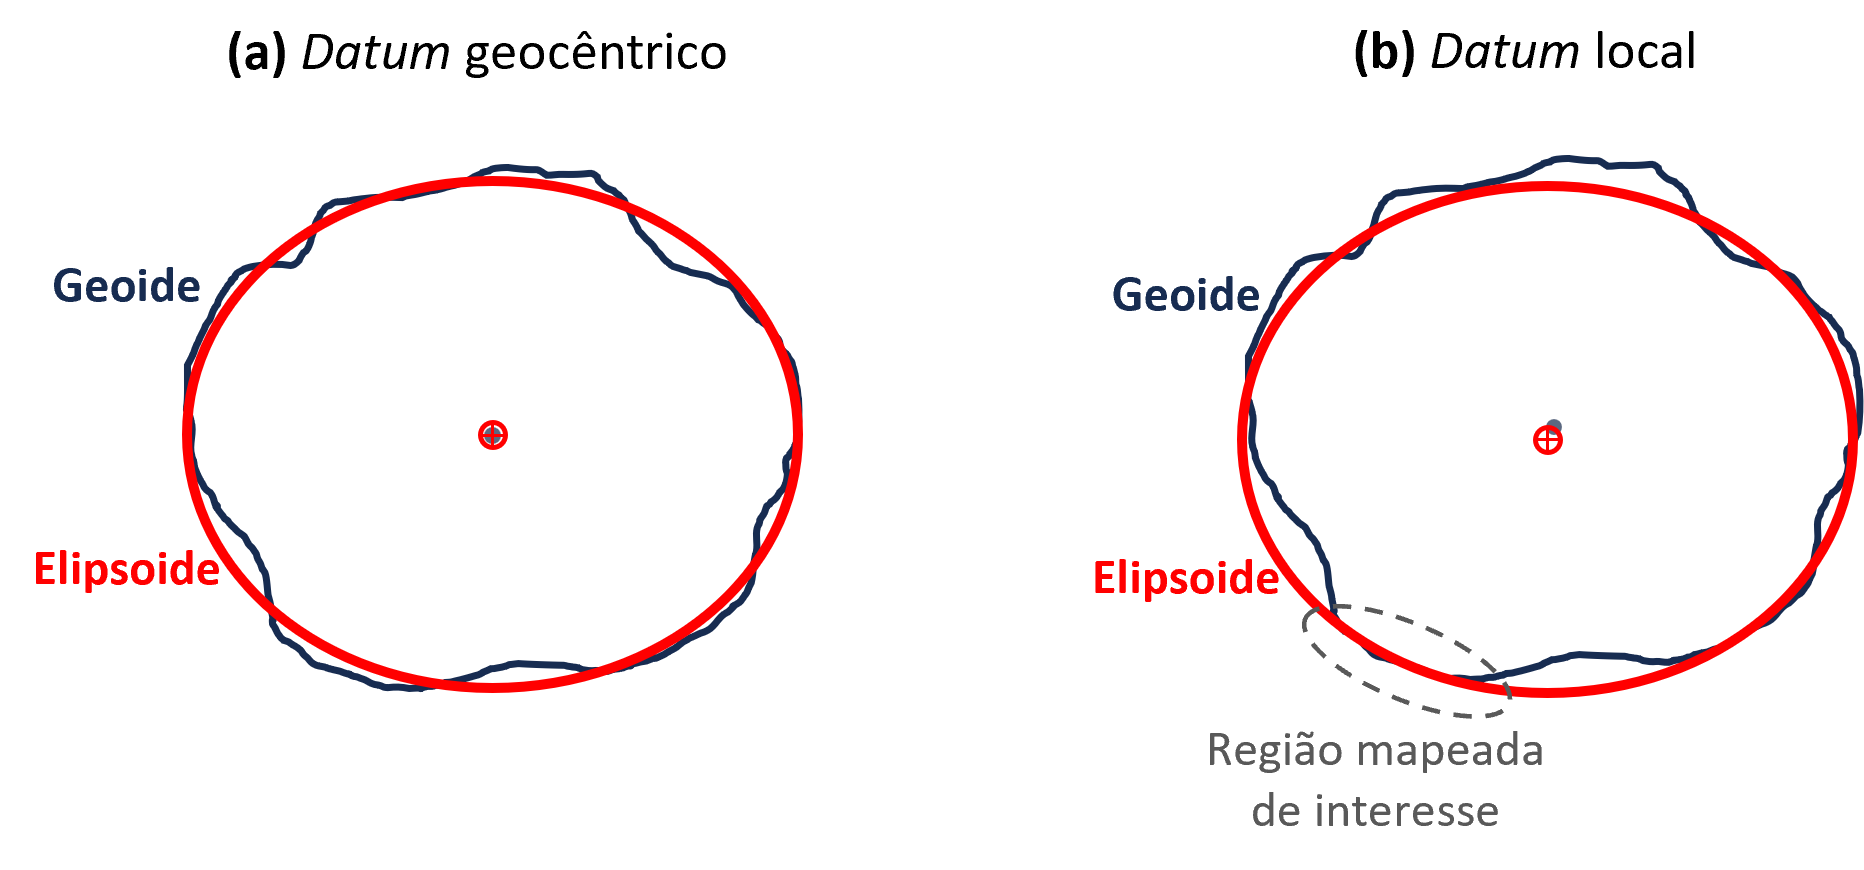
\includegraphics[keepaspectratio]{img/5-dados-geograficos/5-3-datum_loc_geo.png}}

}

\end{figure}%

\subsubsection{Sistema de coordenadas}\label{sistema-de-coordenadas}

O sistema de coordenadas define os eixos e as unidades que permitem
localizar pontos dentro do \emph{datum}, podendo ser de dois tipos
principais: \textbf{geográfico} e \textbf{projetado}. Um sistema de
coordenadas \textbf{geográfico} expressa a posição em latitude e
longitude, medidas em graus. A latitude varia de −90° (polo sul) a +90°
(polo norte), enquanto a longitude varia de −180° a +180°. É o sistema
mais familiar e universal, adotado por GPS, mapas \emph{web} e a maioria
dos arquivos geográficos distribuídos publicamente. Um sistema de
coordenadas \textbf{projetado}, por sua vez, expressa a posição em
coordenadas cartesianas (x e y) sobre um plano, geralmente em metros.
Para chegar a esse plano, é necessária uma projeção cartográfica, o
último aspecto a tratarmos neste tópico de SRC.

\begin{figure}[H]

\caption{\label{fig-src-comparacao}O município de Vitória da
Conquista-BA (em laranja) e seus vizinhos representados em dois sistemas
de referência de coordenadas: geográfico em SIRGAS 2000 (acima), com
eixos em graus de latitude e longitude; e projetado em SIRGAS 2000 / UTM
24S (abaixo), com eixos em metros.}

\centering{

\pandocbounded{
\includegraphics[keepaspectratio]{5-dados-geograficos_files/figure-pdf/fig-src-comparacao-1.pdf}}

}

\end{figure}%

\subsubsection{Projeção
cartográfica}\label{projeuxe7uxe3o-cartogruxe1fica}

A Terra é esférica, mas um mapa é plano. Para representar a superfície
curva do planeta em duas dimensões, é preciso deformá-la
matematicamente. Esse processo é o que se chama de projeção
cartográfica. Toda projeção introduz distorções inevitáveis, e cada tipo
prioriza preservar uma ou duas propriedades geométricas (área, forma,
distância ou direção) às custas das demais.

As projeções são classificadas pela superfície geométrica usada como
intermediária entre o globo e o plano (Figura~\ref{fig-projecoes}). Na
\textbf{projeção azimutal} (ou plana), projeta-se a superfície terrestre
sobre um plano tangente ao globo, geralmente no polo. O resultado é um
mapa circular centrado no ponto de tangência, com distorções crescentes
à medida que se afasta do centro. Na \textbf{projeção cônica},
envolve-se o globo com um cone que o toca ao longo de um ou dois
paralelos; ao se abrir o cone em um plano, obtém-se um mapa em forma de
setor, com distorções menores próximas aos paralelos de tangência. Na
\textbf{projeção cilíndrica}, o globo é envolvido por um cilindro; ao
abri-lo, obtém-se um mapa retangular. A projeção de Mercator (talvez a
mais conhecida) é cilíndrica e preserva formas e ângulos locais, sendo
útil para navegação. Apesar disso, distorce severamente a propriedade de
área. Por exemplo, a Groenlândia aparece com área similar à da África,
embora tenha apenas 7\% da área continental africana.

\begin{figure}[H]

\caption{\label{fig-projecoes}Três famílias de projeções cartográficas:
azimutal (esquerda), cônica (centro) e cilíndrica (direita). Em cada
caso, a superfície geométrica é tangente ao globo e depois planificada,
gerando o mapa correspondente. Fonte:
\href{https://gistbok-topics.ucgis.org/CV-03-006}{UCGIS GIS\&T Body of
Knowledge}.}

\centering{

\pandocbounded{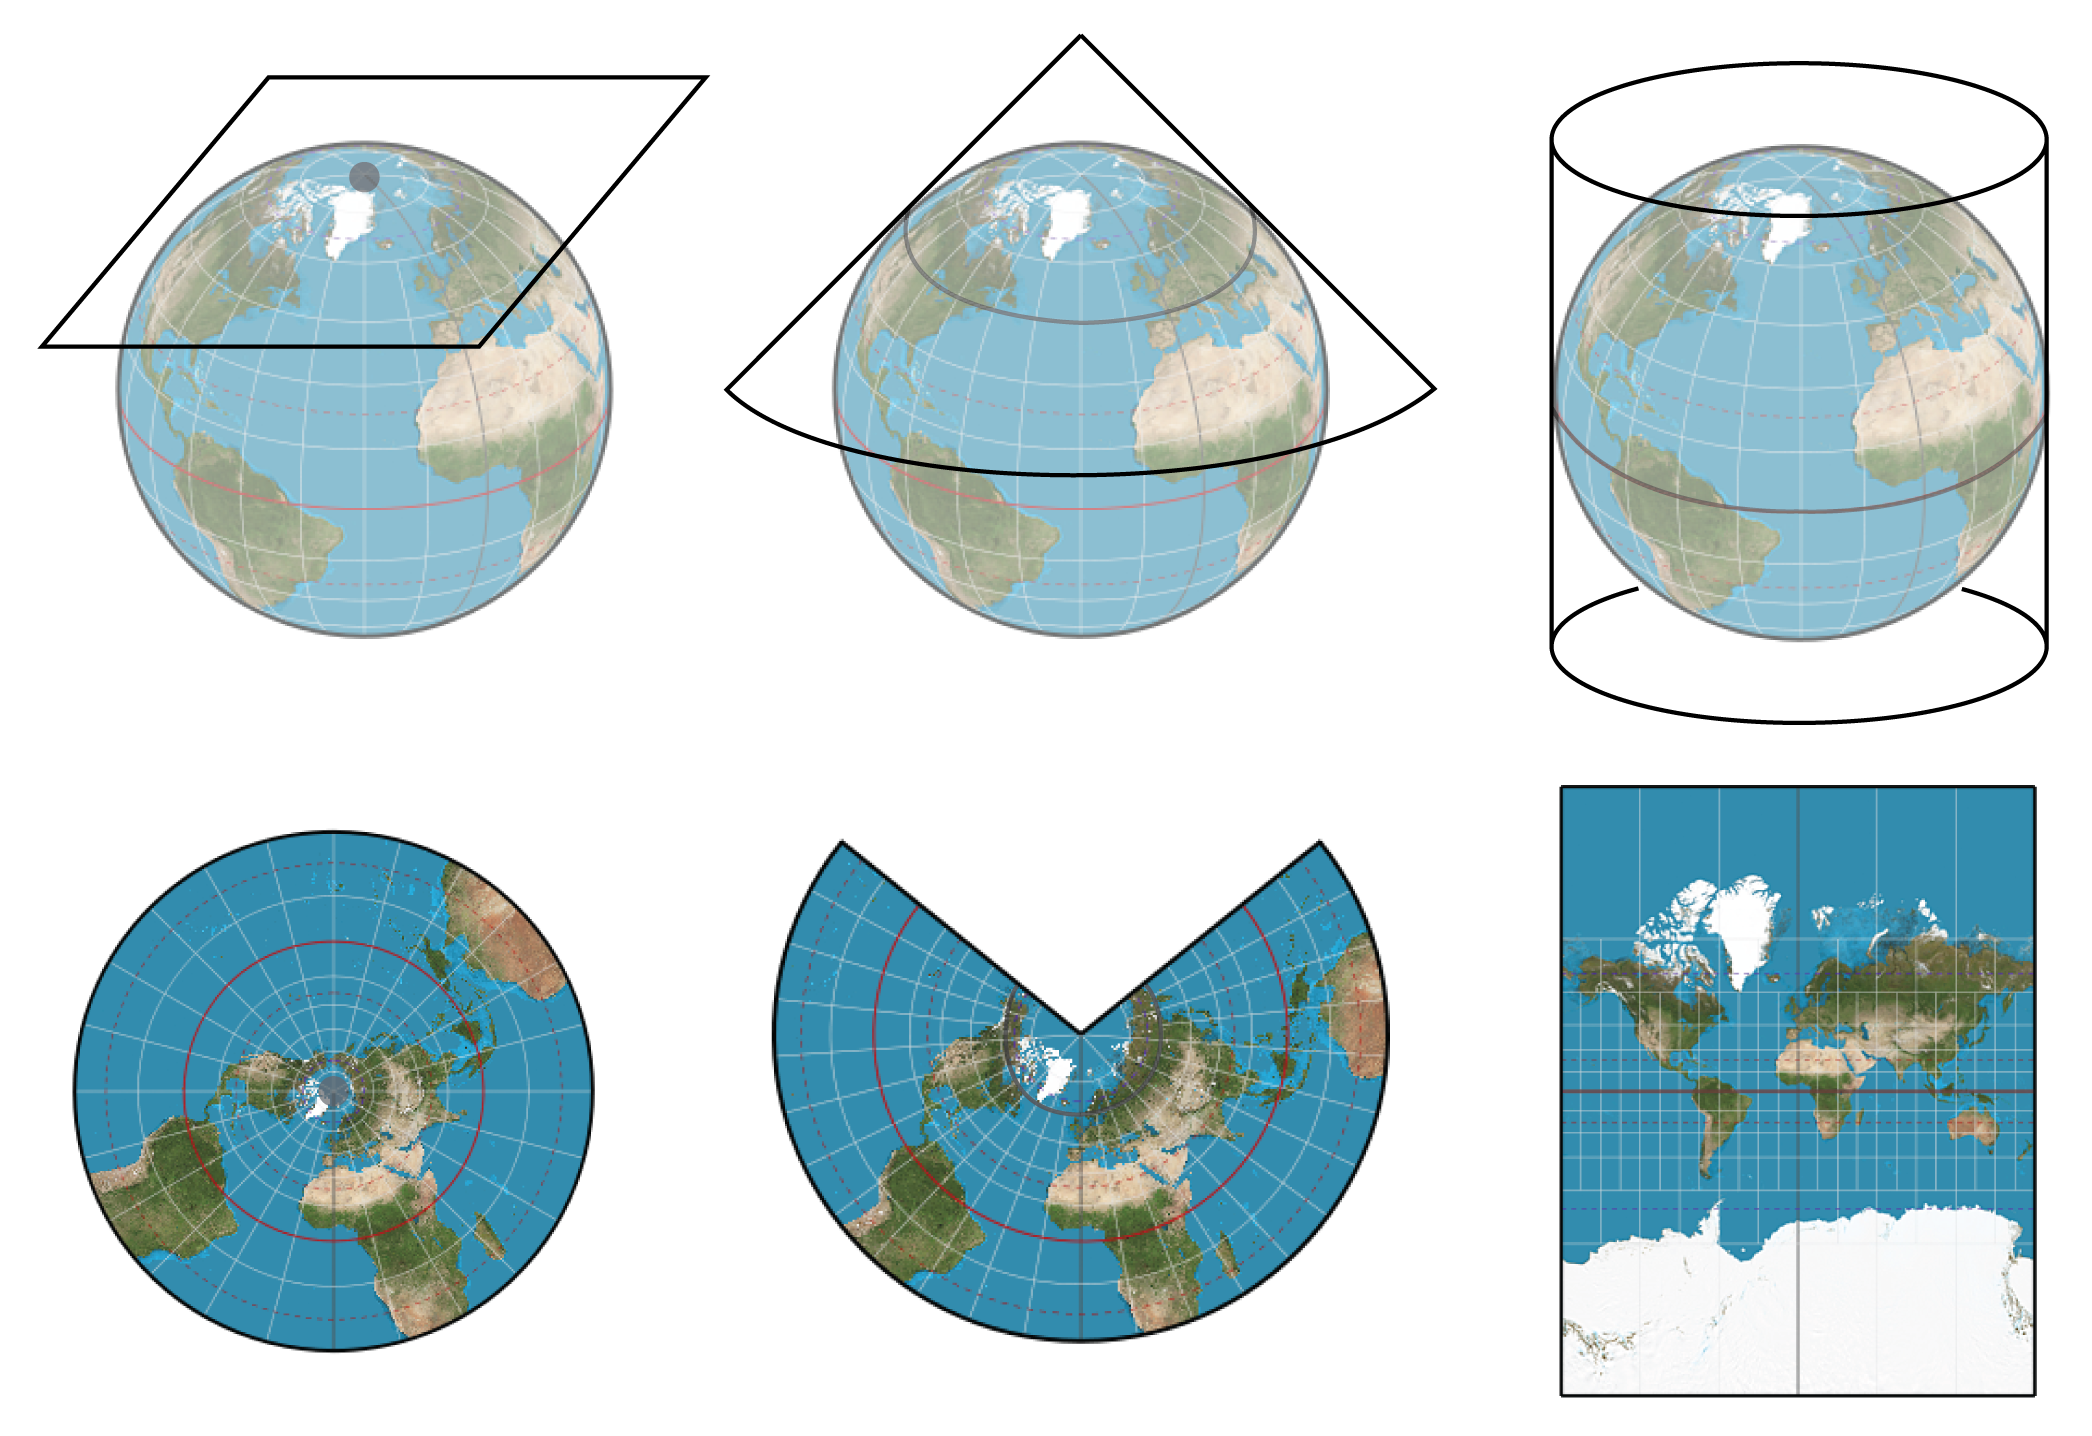
\includegraphics[keepaspectratio]{img/5-dados-geograficos/5-5-projecoes.png}}

}

\end{figure}%

Uma outra projeção bastante notória e que utilizaremos bastante é a UTM
(\emph{Universal Transverse Mercator}), do tipo cilíndrica, mas aplicada
de forma transversal e segmentada. Em vez de um único cilindro
envolvendo o mundo inteiro, o UTM divide o globo em 60 fusos verticais
de 6° de longitude cada, numerados de 1 a 60
(\href{https://gisgeography.com/utm-universal-transverse-mercator-projection/}{GIS
Geography}). Para cada fuso, aplica-se um cilindro transversal que
minimiza as distorções naquela faixa estreita.

\begin{figure}[H]

\caption{\label{fig-utm-cilindro-zonas}Cilindro secante aplicado a um
fuso UTM (a) e as 60 zonas UTM distribuídas ao longo de todo o globo
(b). Fonte:
\href{https://gisgeography.com/utm-universal-transverse-mercator-projection/}{GIS
Geography}.}

\centering{

\pandocbounded{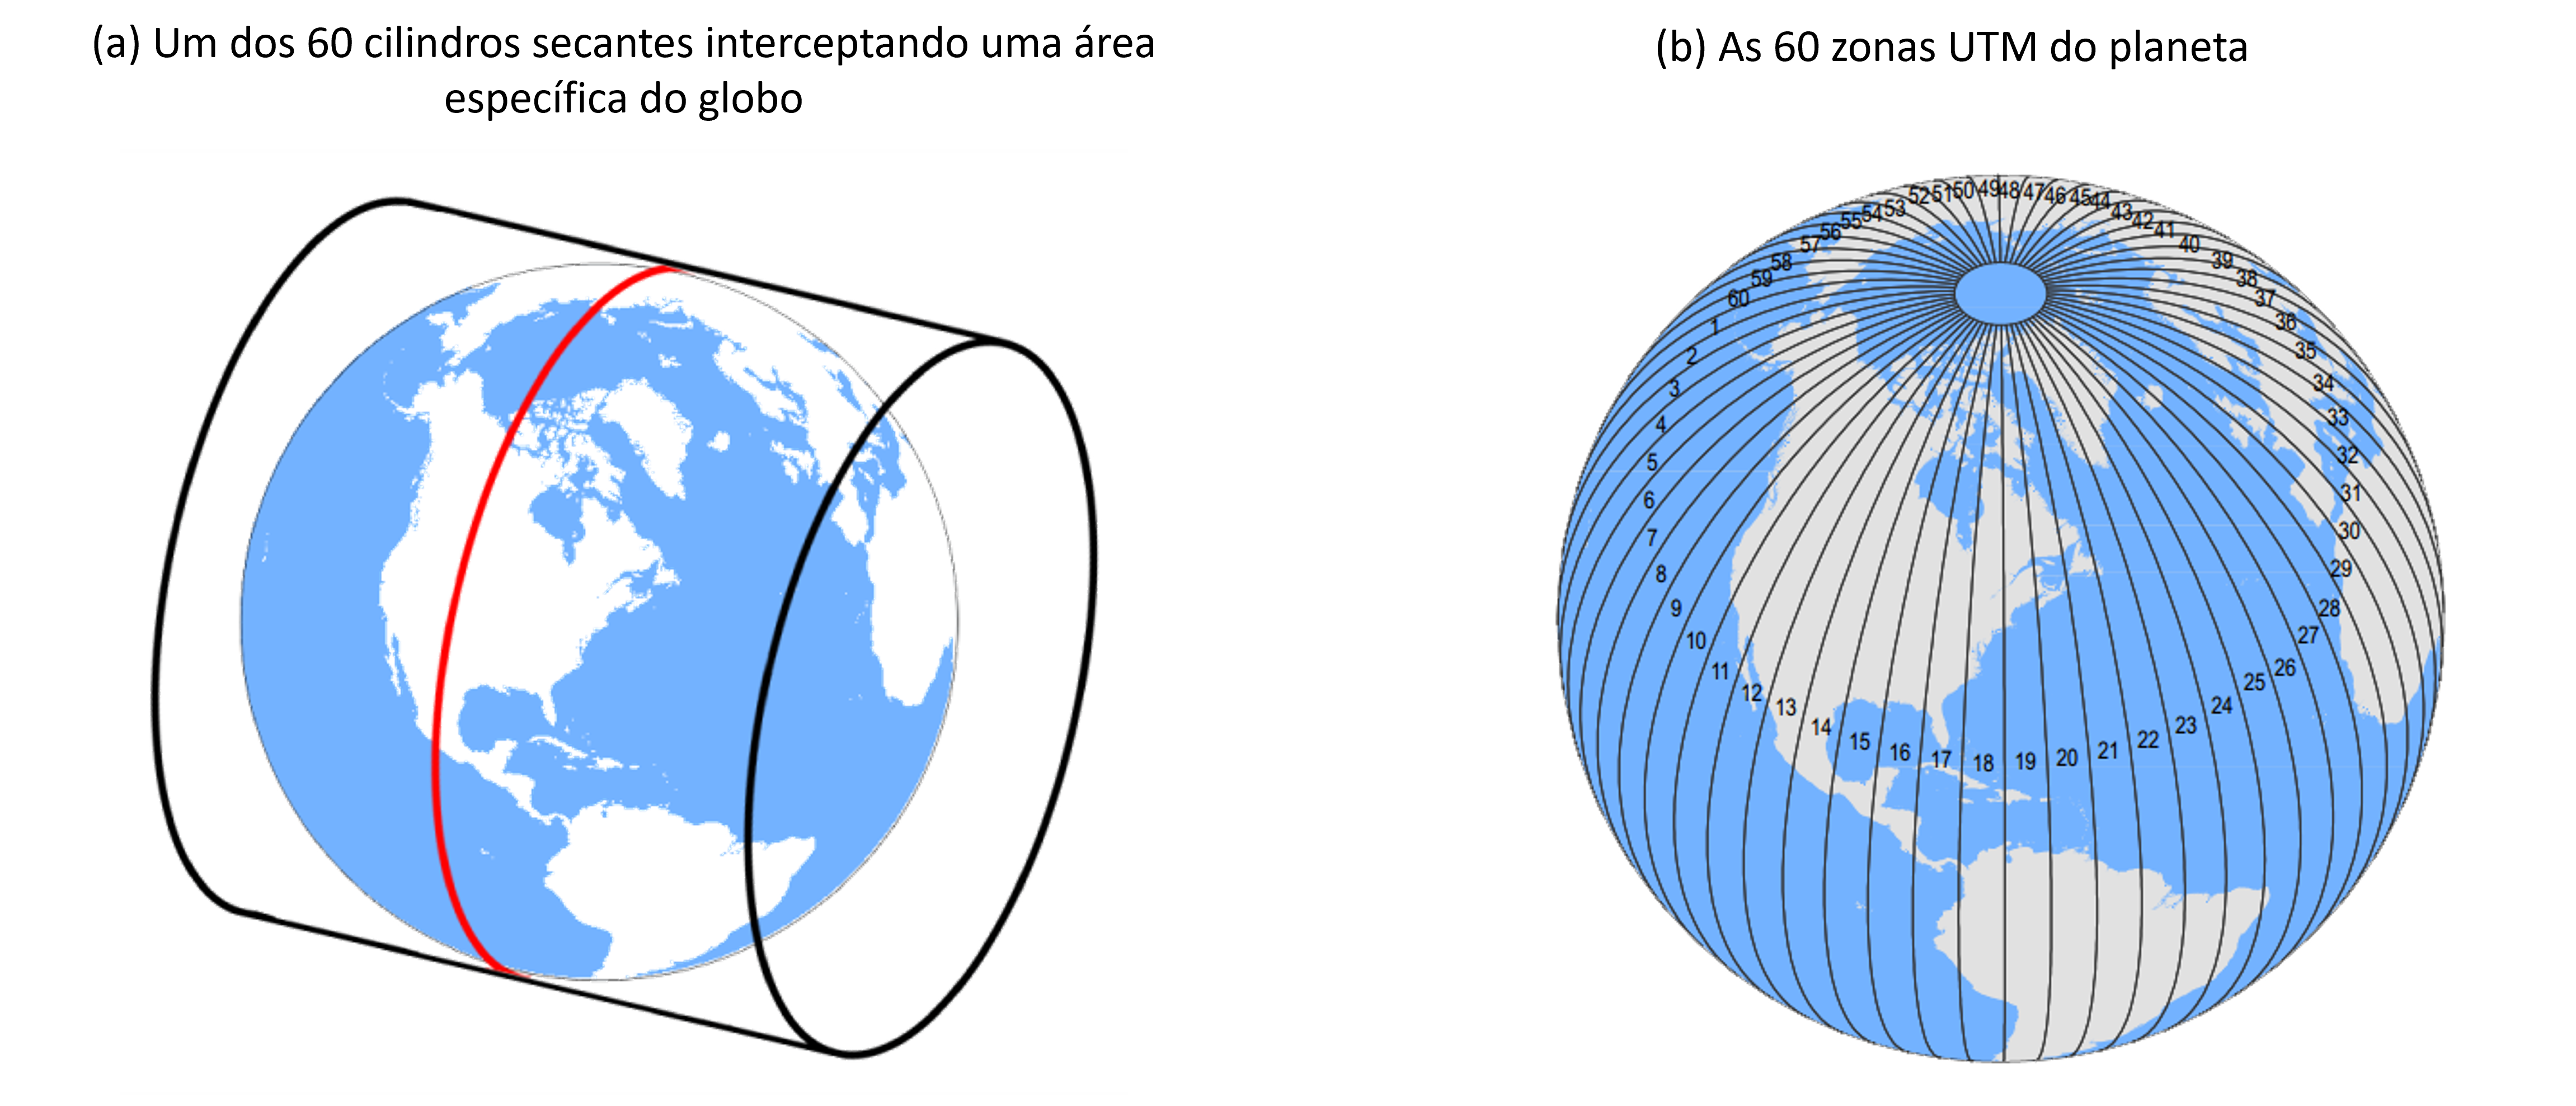
\includegraphics[keepaspectratio]{img/5-dados-geograficos/5-6-utm_cilindro_zonas.png}}

}

\end{figure}%

O Brasil ocupa principalmente os fusos 18 a 25, e a escolha do fuso
correto é essencial para que distâncias e áreas sejam matematicamente
precisas. No exemplo da Figura~\ref{fig-src-comparacao} anterior, por
exemplo, escolhemos o UTM 24S, pois é o fuso UTM onde o município de
Vitória da Conquista-BA se localiza.

\begin{figure}[H]

\caption{\label{fig-utm-brasil}Fusos UTM de 18 a 25 sobrepostos ao
território brasileiro, subdivididos em Norte (N) e Sul (S) pelo equador.
Cada fuso abrange 6° de longitude.}

\centering{

\pandocbounded{
\includegraphics[keepaspectratio]{5-dados-geograficos_files/figure-pdf/fig-utm-brasil-1.pdf}}

}

\end{figure}%

Na prática, para visualização de áreas extensas (ex.: estados inteiros)
e intercâmbio de dados, o SRC geográfico (lat/lon em graus) é o mais
conveniente. Para análises quantitativas que envolvam medição de
distâncias, cálculo de áreas ou criação de zonas de influência, é
necessário um SRC projetado com unidades métricas.

\subsubsection{Codificação EPSG}\label{codificauxe7uxe3o-epsg}

Com centenas de sistemas de referência disponíveis, é preciso uma forma
padronizada de identificá-los. A IOGP (\emph{International Association
of Oil \& Gas Producers}, antiga \emph{European Petroleum Survey Group})
publica o EPSG Geodetic Parameter Dataset, um banco de dados que atribui
um código numérico único a cada SRC, \emph{datum}, elipsoide e operação
de transformação registrados.

Os códigos EPSG aparecem frequentemente em arquivos geográficos e
funções de geoprocessamento. A tabela abaixo reúne os mais relevantes
para as análises com dados brasileiros.

{\def\LTcaptype{none} % do not increment counter
\begin{longtable}[]{@{}llll@{}}
\toprule\noalign{}
Código EPSG & SRC & Tipo & Unidade \\
\midrule\noalign{}
\endhead
\bottomrule\noalign{}
\endlastfoot
4326 & WGS84 & Geográfico & Graus \\
4674 & SIRGAS 2000 & Geográfico & Graus \\
31983 & SIRGAS 2000 / UTM fuso 23S & Projetado & Metros \\
31984 & SIRGAS 2000 / UTM fuso 24S & Projetado & Metros \\
5880 & SIRGAS 2000 / Policônico & Projetado & Metros \\
3857 & Web Mercator & Projetado & Metros \\
\end{longtable}
}

Com os conceitos de SRC estabelecidos, é possível avançar para o lado
prático sobre como trabalhar com dados geográficos no R, tema das nossas
próximas seções.

\section{\texorpdfstring{Dados vetoriais e o pacote \texttt{sf} para
R}{Dados vetoriais e o pacote sf para R}}\label{dados-vetoriais-e-o-pacote-sf-para-r}

O pacote \texttt{sf} (\emph{simple features}) é a principal biblioteca
para dados geográficos \textbf{vetoriais} no R. Ele implementa o padrão
ISO 19125, conhecido como \emph{Simple Features}, que define como
representar e operar sobre geometrias vetoriais de forma consistente.
Internamente, o \texttt{sf} se apoia em quatro bibliotecas escritas em
C++:

\begin{itemize}
\tightlist
\item
  \textbf{GDAL} (\emph{Geospatial Data Abstraction Library}): leitura e
  escrita de dezenas de formatos geográficos, como GeoPackage, GeoJSON,
  Shapefile e outros.
\item
  \textbf{GEOS} (\emph{Geometry Engine, Open Source}): operações
  geométricas como buffers, interseções e uniões em coordenadas
  projetadas.
\item
  \textbf{PROJ}: transformações entre sistemas de referência de
  coordenadas.
\item
  \textbf{s2geometry}: operações geométricas em coordenadas geográficas
  (longitude/latitude), tratando a Terra como uma esfera. Usada por
  padrão desde a versão 1.0 do \texttt{sf}.
\end{itemize}

Em geoprocessamento, uma \textbf{camada vetorial} é um conjunto de
feições do mesmo tipo geométrico, organizado como uma tabela. Os três
componentes fundamentais de uma camada vetorial são:

\begin{itemize}
\tightlist
\item
  \textbf{Feição} (\emph{feature}): cada linha da tabela corresponde a
  uma feição (um elemento geográfico individual), como um município, um
  trecho de rodovia ou uma escola. Cada feição tem uma geometria e um
  conjunto de atributos.
\item
  \textbf{Campos} (\emph{fields}) ou \textbf{atributos}: as colunas
  não-espaciais da tabela, que descrevem características de cada feição
  (nome, código, população, área, etc.). No R, são acessados como
  colunas normais de um \emph{data frame}.
\item
  \textbf{Geometria}: a coluna especial que armazena a representação
  espacial de cada feição (ponto, linha ou polígono). No \texttt{sf},
  essa coluna é da classe \texttt{sfc} e geralmente se chama
  \texttt{geometry} ou \texttt{geom}.
\end{itemize}

Além desses três componentes, toda camada vetorial carrega
\textbf{metadados} que descrevem suas propriedades globais. Eles
aparecem automaticamente ao imprimir um objeto \texttt{sf}. Os metadados
incluem o número de feições e campos, o tipo de geometria, a caixa
delimitadora e o sistema de referência de coordenadas.

O objeto \texttt{sf} de uma camada vetorial comporta-se essencialmente
como um \emph{data frame}. Isso significa que todas as operações do
\texttt{dplyr} (\texttt{filter()}, \texttt{mutate()},
\texttt{left\_join()} etc.) funcionam diretamente sobre objetos
\texttt{sf}, tornando o fluxo de trabalho coeso com o restante do
\texttt{tidyverse}.

\subsection{Tipos de geometria}\label{tipos-de-geometria}

O padrão \emph{Simple Features} define 18 tipos de geometria. Na
prática, utilizamos mais as seis primeiras das sete principais abaixo,
ilustradas na Figura~\ref{fig-tipos-geometria}:

\begin{itemize}
\tightlist
\item
  \texttt{POINT}: um único ponto (uma escola, uma estação de metrô).
\item
  \texttt{LINESTRING}: uma sequência de pontos conectados (uma rua, uma
  linha de metrô).
\item
  \texttt{POLYGON}: uma área fechada (um bairro, um município).
\item
  \texttt{MULTIPOINT}: coleção de pontos pertencentes à mesma feição.
\item
  \texttt{MULTILINESTRING}: coleção de linhas pertencentes à mesma
  feição (ex.: ruas descontínuas).
\item
  \texttt{MULTIPOLYGON}: coleção de polígonos pertencentes à mesma
  feição (um estado com ilhas, por exemplo).
\item
  \texttt{GEOMETRYCOLLECTION}: mistura de tipos geométricos em uma única
  feição.
\end{itemize}

\begin{figure}[H]

\caption{\label{fig-tipos-geometria}Tipos de geometria do padrão
\emph{Simple Features} e a relação entre eles.}

\centering{

\pandocbounded{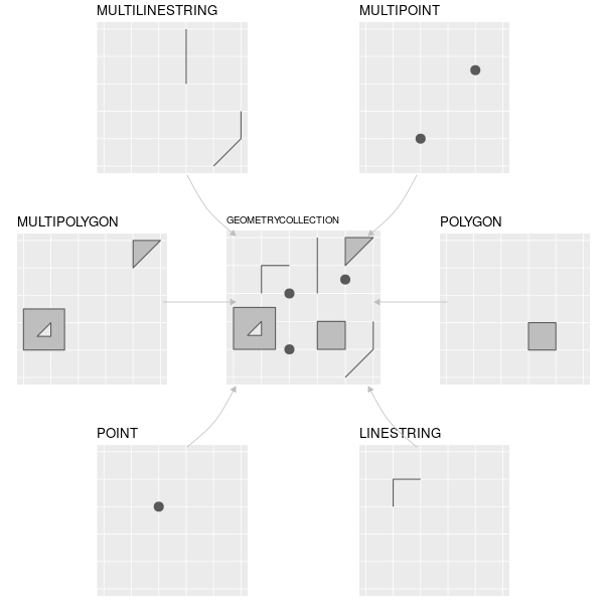
\includegraphics[keepaspectratio]{img/5-dados-geograficos/5-8-tipos_geometria.png}}

}

\end{figure}%

Cada tipo tem uma representação textual padronizada chamada \emph{WKT}
(\emph{Well-Known Text}), útil para inspecionar objetos \texttt{sf},
construir geometrias manualmente e trocar dados entre sistemas
diferentes. A função \texttt{st\_as\_sfc()} converte uma \emph{string}
WKT (no formato de texto, entre aspas) em um objeto de geometria do
\texttt{sf}.

Um \texttt{POINT} é o tipo mais simples: um único par de coordenadas x y
separadas por espaço, onde x corresponde à longitude e y à latitude:

\begin{Shaded}
\begin{Highlighting}[]
\FunctionTok{st\_as\_sfc}\NormalTok{(}\StringTok{"POINT ({-}38.51 {-}12.96)"}\NormalTok{)}
\end{Highlighting}
\end{Shaded}

\begin{verbatim}
Geometry set for 1 feature 
Geometry type: POINT
Dimension:     XY
Bounding box:  xmin: -38.51 ymin: -12.96 xmax: -38.51 ymax: -12.96
CRS:           NA
\end{verbatim}

Um \texttt{LINESTRING} é uma sequência de pares x y separados por
vírgula. O \texttt{sf} os conecta em ordem, formando segmentos de reta
para uma mesma linha:

\begin{Shaded}
\begin{Highlighting}[]
\FunctionTok{st\_as\_sfc}\NormalTok{(}\StringTok{"LINESTRING ({-}38.51 {-}12.96, {-}38.49 {-}12.97, {-}38.48 {-}13.00)"}\NormalTok{)}
\end{Highlighting}
\end{Shaded}

\begin{verbatim}
Geometry set for 1 feature 
Geometry type: LINESTRING
Dimension:     XY
Bounding box:  xmin: -38.51 ymin: -13 xmax: -38.48 ymax: -12.96
CRS:           NA
\end{verbatim}

Um \texttt{POLYGON} define uma área fechada por um anel de coordenadas.
Por isso, o último par deve ser idêntico ao primeiro. Os quatro pares
únicos abaixo definem os três cantos de um triângulo, sendo que o quarto
par fecha o anel voltando ao ponto de origem. Os parênteses são duplos
porque o padrão WKT reserva os parênteses internos para representar
furos no polígono (não utilizados no exemplo abaixo).

\begin{Shaded}
\begin{Highlighting}[]
\FunctionTok{st\_as\_sfc}\NormalTok{(}\StringTok{"POLYGON (({-}38.52 {-}12.95, {-}38.47 {-}12.95, {-}38.47 {-}13.01, {-}38.52 {-}12.95))"}\NormalTok{)}
\end{Highlighting}
\end{Shaded}

\begin{verbatim}
Geometry set for 1 feature 
Geometry type: POLYGON
Dimension:     XY
Bounding box:  xmin: -38.52 ymin: -13.01 xmax: -38.47 ymax: -12.95
CRS:           NA
\end{verbatim}

Um \texttt{MULTIPOINT} reúne dois ou mais pontos em uma única feição.
Cada ponto fica entre seus próprios parênteses internos. O importante é
que, na tabela, os dois pontos abaixo correspondem a uma só linha da
tabela (uma única feição com duas localizações):

\begin{Shaded}
\begin{Highlighting}[]
\FunctionTok{st\_as\_sfc}\NormalTok{(}\StringTok{"MULTIPOINT (({-}38.51 {-}12.96),}
\StringTok{                       ({-}38.49 {-}12.97))"}\NormalTok{)}
\end{Highlighting}
\end{Shaded}

\begin{verbatim}
Geometry set for 1 feature 
Geometry type: MULTIPOINT
Dimension:     XY
Bounding box:  xmin: -38.51 ymin: -12.97 xmax: -38.49 ymax: -12.96
CRS:           NA
\end{verbatim}

Um \texttt{MULTILINESTRING} reúne dois ou mais trechos de linha em uma
única feição. Cada trecho fica entre seus próprios parênteses. O exemplo
abaixo cria uma feição com dois segmentos, como os dois sentidos de uma
avenida representados como traços separados.

\begin{Shaded}
\begin{Highlighting}[]
\FunctionTok{st\_as\_sfc}\NormalTok{(}\StringTok{"MULTILINESTRING (({-}38.51 {-}12.96, {-}38.49 {-}12.97),}
\StringTok{                            ({-}38.48 {-}13.00, {-}38.47 {-}13.01))"}\NormalTok{)}
\end{Highlighting}
\end{Shaded}

\begin{verbatim}
Geometry set for 1 feature 
Geometry type: MULTILINESTRING
Dimension:     XY
Bounding box:  xmin: -38.51 ymin: -13.01 xmax: -38.47 ymax: -12.96
CRS:           NA
\end{verbatim}

Um \texttt{MULTIPOLYGON} reúne dois ou mais polígonos em uma única
feição. É o tipo mais frequente nas bases brasileiras. Estados e
municípios com ilhas têm o território continental e as ilhas como
polígonos distintos, mas compõem uma única feição na tabela. Cada
polígono fica entre parênteses duplos (o nível interno reservado ao
anel, o externo ao agrupamento), resultando em três níveis de parênteses
no total.

\begin{Shaded}
\begin{Highlighting}[]
\FunctionTok{st\_as\_sfc}\NormalTok{(}\StringTok{"MULTIPOLYGON ((({-}38.52 {-}12.95, {-}38.47 {-}12.95, {-}38.47 {-}13.01, {-}38.52 {-}12.95)),}
\StringTok{                         (({-}38.45 {-}12.94, {-}38.43 {-}12.94, {-}38.43 {-}12.96, {-}38.45 {-}12.94)))"}\NormalTok{)}
\end{Highlighting}
\end{Shaded}

\begin{verbatim}
Geometry set for 1 feature 
Geometry type: MULTIPOLYGON
Dimension:     XY
Bounding box:  xmin: -38.52 ymin: -13.01 xmax: -38.43 ymax: -12.94
CRS:           NA
\end{verbatim}

\subsection{Criando camadas vetoriais do
zero}\label{criando-camadas-vetoriais-do-zero}

Para entender a estrutura de objetos \texttt{sf}, é útil criá-los do
zero. Em vez de descrever geometrias como texto WKT, podemos utilizar
funções do pacote \texttt{sf}, como \texttt{st\_point()},
\texttt{st\_linestring()} e \texttt{st\_polygon()}, que recebem vetores
e matrizes de coordenadas. O resultado de cada uma é um objeto de
geometria individual (\texttt{sfg}), que depois é agrupado em uma coluna
de geometrias com \texttt{st\_sfc()} e associado a um \emph{data frame}
de atributos com \texttt{st\_sf()}, formando uma camada vetorial
completa.

O exemplo abaixo cria três pontos (estações hipotéticas de metrô), uma
linha (o traçado hipotético) e um polígono (um bairro hipotético), todos
referenciados ao \emph{datum} SIRGAS 2000 (EPSG 4674):

\begin{Shaded}
\begin{Highlighting}[]
\CommentTok{\# Três pontos: estações hipotéticas}
\NormalTok{p1 }\OtherTok{\textless{}{-}} \FunctionTok{st\_point}\NormalTok{(}\FunctionTok{c}\NormalTok{(}\SpecialCharTok{{-}}\FloatTok{38.510}\NormalTok{, }\SpecialCharTok{{-}}\FloatTok{12.960}\NormalTok{))}
\NormalTok{p2 }\OtherTok{\textless{}{-}} \FunctionTok{st\_point}\NormalTok{(}\FunctionTok{c}\NormalTok{(}\SpecialCharTok{{-}}\FloatTok{38.495}\NormalTok{, }\SpecialCharTok{{-}}\FloatTok{12.975}\NormalTok{))}
\NormalTok{p3 }\OtherTok{\textless{}{-}} \FunctionTok{st\_point}\NormalTok{(}\FunctionTok{c}\NormalTok{(}\SpecialCharTok{{-}}\FloatTok{38.480}\NormalTok{, }\SpecialCharTok{{-}}\FloatTok{13.005}\NormalTok{))}

\NormalTok{estacoes\_hip }\OtherTok{\textless{}{-}} \FunctionTok{st\_sf}\NormalTok{(}
  \AttributeTok{nome =} \FunctionTok{c}\NormalTok{(}\StringTok{"Estação A"}\NormalTok{, }\StringTok{"Estação B"}\NormalTok{, }\StringTok{"Estação C"}\NormalTok{),}
  \AttributeTok{geometry =} \FunctionTok{st\_sfc}\NormalTok{(p1, p2, p3, }\AttributeTok{crs =} \DecValTok{4674}\NormalTok{)}
\NormalTok{)}

\CommentTok{\# Uma linha: traçado hipotético}
\NormalTok{linha\_hip }\OtherTok{\textless{}{-}} \FunctionTok{st\_sf}\NormalTok{(}
  \AttributeTok{nome =} \StringTok{"Linha Hipotética"}\NormalTok{,}
  \AttributeTok{geometry =} \FunctionTok{st\_sfc}\NormalTok{(}
    \FunctionTok{st\_linestring}\NormalTok{(}
      \FunctionTok{matrix}\NormalTok{(}\FunctionTok{c}\NormalTok{(}\SpecialCharTok{{-}}\FloatTok{38.510}\NormalTok{, }\SpecialCharTok{{-}}\FloatTok{12.960}\NormalTok{,}
               \SpecialCharTok{{-}}\FloatTok{38.495}\NormalTok{, }\SpecialCharTok{{-}}\FloatTok{12.975}\NormalTok{,}
               \SpecialCharTok{{-}}\FloatTok{38.480}\NormalTok{, }\SpecialCharTok{{-}}\FloatTok{13.005}\NormalTok{),}
             \AttributeTok{ncol =} \DecValTok{2}\NormalTok{, }\AttributeTok{byrow =} \ConstantTok{TRUE}\NormalTok{)}
\NormalTok{    ),}
    \AttributeTok{crs =} \DecValTok{4674}
\NormalTok{  )}
\NormalTok{)}

\CommentTok{\# Um polígono: bairro hipotético}
\NormalTok{poligono\_hip }\OtherTok{\textless{}{-}} \FunctionTok{st\_sf}\NormalTok{(}
  \AttributeTok{nome =} \StringTok{"Bairro Hipotético"}\NormalTok{,}
  \AttributeTok{geometry =} \FunctionTok{st\_sfc}\NormalTok{(}
    \FunctionTok{st\_polygon}\NormalTok{(}\FunctionTok{list}\NormalTok{(}
      \FunctionTok{matrix}\NormalTok{(}\FunctionTok{c}\NormalTok{(}\SpecialCharTok{{-}}\FloatTok{38.520}\NormalTok{, }\SpecialCharTok{{-}}\FloatTok{12.950}\NormalTok{,}
               \SpecialCharTok{{-}}\FloatTok{38.470}\NormalTok{, }\SpecialCharTok{{-}}\FloatTok{12.950}\NormalTok{,}
               \SpecialCharTok{{-}}\FloatTok{38.470}\NormalTok{, }\SpecialCharTok{{-}}\FloatTok{13.015}\NormalTok{,}
               \SpecialCharTok{{-}}\FloatTok{38.520}\NormalTok{, }\SpecialCharTok{{-}}\FloatTok{13.015}\NormalTok{,}
               \SpecialCharTok{{-}}\FloatTok{38.520}\NormalTok{, }\SpecialCharTok{{-}}\FloatTok{12.950}\NormalTok{),}
             \AttributeTok{ncol =} \DecValTok{2}\NormalTok{, }\AttributeTok{byrow =} \ConstantTok{TRUE}\NormalTok{)}
\NormalTok{    )),}
    \AttributeTok{crs =} \DecValTok{4674}
\NormalTok{  )}
\NormalTok{)}
\end{Highlighting}
\end{Shaded}

O resultado das operações anteriores produzem os seguintes arquivos
geográficos abaixo, que aprenderemos a visualizar em R logo mais:

\begin{figure}[H]

\caption{\label{fig-geometrias-scratch}Objeto \texttt{sf} criado do zero
com três tipos de geometria: um polígono, uma linha e três pontos ---
todos referenciados ao datum SIRGAS 2000.}

\centering{

\pandocbounded{
\includegraphics[keepaspectratio]{5-dados-geograficos_files/figure-pdf/fig-geometrias-scratch-1.pdf}}

}

\end{figure}%

Dois aspectos merecem atenção. Primeiro, o SRC é definido no momento da
criação (\texttt{crs\ =\ 4674}). Sem ele, o objeto \texttt{sf}
existiria, mas seria espacialmente indefinido. Segundo, a estrutura
resultante é um \emph{data frame} comum: \texttt{estacoes\_hip} tem
linhas (uma por estação), colunas de atributos (\texttt{nome}) e uma
coluna de geometria.

\subsection{Lendo Arquivos
Geográficos}\label{lendo-arquivos-geogruxe1ficos}

Mais comum do que criarmos arquivos geográficos do zero é lermos
arquivos existentes de alguma base de dados. Eles podem assumir diversos
formatos (extensões) predefinidos, como GeoPackage (\texttt{.gpkg}),
GeoJSON (\texttt{.geojson}), Shapefile (\texttt{.shp}), entre outros. A
função \texttt{st\_read()} lê qualquer um desses formatos e devolve um
objeto \texttt{sf}.

Antes de prosseguir com o código abaixo, lembre-se de fazer o download
dos arquivos listados no início do capítulo, salve-os em uma pasta e
inicie um porjeto no RStudio\footnote{se você estiver usando Positron,
  esta etapa não é necessária}. Na sequência, em um script \texttt{.R},
use os comandos abaixo para carregá-los:

\begin{Shaded}
\begin{Highlighting}[]
\FunctionTok{library}\NormalTok{(tidyverse)}
\FunctionTok{library}\NormalTok{(sf)}

\NormalTok{uf\_br   }\OtherTok{\textless{}{-}} \FunctionTok{st\_read}\NormalTok{(}\StringTok{"uf\_br.gpkg"}\NormalTok{)}
\NormalTok{ssa     }\OtherTok{\textless{}{-}} \FunctionTok{st\_read}\NormalTok{(}\StringTok{"ssa.gpkg"}\NormalTok{)}
\NormalTok{bairros }\OtherTok{\textless{}{-}} \FunctionTok{st\_read}\NormalTok{(}\StringTok{"bairros\_ssa.geojson"}\NormalTok{)}
\NormalTok{escolas }\OtherTok{\textless{}{-}} \FunctionTok{st\_read}\NormalTok{(}\StringTok{"escolas\_ssa.gpkg"}\NormalTok{)}
\NormalTok{est\_metro }\OtherTok{\textless{}{-}} \FunctionTok{st\_read}\NormalTok{(}\StringTok{"smsl\_est.gpkg"}\NormalTok{)}
\NormalTok{lin\_metro }\OtherTok{\textless{}{-}} \FunctionTok{st\_read}\NormalTok{(}\StringTok{"smsl\_linhas.gpkg"}\NormalTok{)}
\NormalTok{pop\_uf  }\OtherTok{\textless{}{-}} \FunctionTok{read\_csv}\NormalTok{(}\StringTok{"pop\_uf\_br.csv"}\NormalTok{)}
\end{Highlighting}
\end{Shaded}

Após carregar, use \texttt{st\_crs()} para inspecionar o SRC de qualquer
objeto:

\begin{Shaded}
\begin{Highlighting}[]
\FunctionTok{st\_crs}\NormalTok{(uf\_br)}
\end{Highlighting}
\end{Shaded}

\begin{verbatim}
Coordinate Reference System:
  User input: SIRGAS 2000 
  wkt:
GEOGCRS["SIRGAS 2000",
    DATUM["Sistema de Referencia Geocentrico para las AmericaS 2000",
        ELLIPSOID["GRS 1980",6378137,298.257222101,
            LENGTHUNIT["metre",1]]],
    PRIMEM["Greenwich",0,
        ANGLEUNIT["degree",0.0174532925199433]],
    CS[ellipsoidal,2],
        AXIS["geodetic latitude (Lat)",north,
            ORDER[1],
            ANGLEUNIT["degree",0.0174532925199433]],
        AXIS["geodetic longitude (Lon)",east,
            ORDER[2],
            ANGLEUNIT["degree",0.0174532925199433]],
    USAGE[
        SCOPE["Horizontal component of 3D system."],
        AREA["Latin America - Central America and South America - onshore and offshore. Brazil - onshore and offshore."],
        BBOX[-59.87,-122.19,32.72,-25.28]],
    ID["EPSG",4674]]
\end{verbatim}

Note que o \emph{output} acima gera diversos metadados relativos ao SRC
do objeto espacial. Se quisermos de forma específica somente o código
EPSG do SRC da camada, podemos fazer:

\begin{Shaded}
\begin{Highlighting}[]
\FunctionTok{st\_crs}\NormalTok{(uf\_br)}\SpecialCharTok{$}\NormalTok{epsg}
\end{Highlighting}
\end{Shaded}

\begin{verbatim}
[1] 4674
\end{verbatim}

\begin{Shaded}
\begin{Highlighting}[]
\FunctionTok{st\_crs}\NormalTok{(bairros)}\SpecialCharTok{$}\NormalTok{epsg}
\end{Highlighting}
\end{Shaded}

\begin{verbatim}
[1] 4326
\end{verbatim}

\begin{Shaded}
\begin{Highlighting}[]
\FunctionTok{st\_crs}\NormalTok{(escolas)}\SpecialCharTok{$}\NormalTok{epsg}
\end{Highlighting}
\end{Shaded}

\begin{verbatim}
[1] 4674
\end{verbatim}

Observe que os estados do Brasil (\texttt{uf\_br}) e as escolas
(\texttt{escolas}) estão em SIRGAS 2000 (EPSG 4674). Os bairros de
Salvador (\texttt{bairros}) estão em WGS84 (EPSG 4326). Essa diferença
de SRC entre camadas é algo a ser observado antes de qualquer operação
que combine duas ou mais delas.

\subsection{Visualizando Dados
Geográficos}\label{visualizando-dados-geogruxe1ficos}

É possível plotar esses arquivos geográficos com apoio do pacote
\texttt{ggplot2}, oriundo da família de pacotes \texttt{tidyverse}, que
já vimos no capítulo anterior. Para tanto, utilizaremos a função
\texttt{geom\_sf()} para mapeá-los de maneira sobreposta, conforme o
exemplo abaixo. É importante destacar que o \texttt{ggplot2} reconhece
objetos \texttt{sf} automaticamente por meio da função
\texttt{geom\_sf()}.

Comecemos com o mapa de estados armazenado no objeto \texttt{sf}
denominado \texttt{uf\_br}, que contém feições (polígonos) relativos a
cada estado do Brasil. Antes de plotá-lo, vale examinar sua estrutura:

\begin{Shaded}
\begin{Highlighting}[]
\NormalTok{uf\_br}
\end{Highlighting}
\end{Shaded}

\begin{verbatim}
Simple feature collection with 27 features and 5 fields
Geometry type: MULTIPOLYGON
Dimension:     XY
Bounding box:  xmin: -73.99045 ymin: -33.75208 xmax: -28.83591 ymax: 5.271841
Geodetic CRS:  SIRGAS 2000
First 10 features:
   code_state abbrev_state name_state code_region name_region
1          11           RO   Rondônia           1       Norte
2          12           AC       Acre           1       Norte
3          13           AM   Amazonas           1       Norte
4          14           RR    Roraima           1       Norte
5          15           PA       Pará           1       Norte
6          16           AP      Amapá           1       Norte
7          17           TO  Tocantins           1       Norte
8          21           MA   Maranhão           2    Nordeste
9          22           PI      Piauí           2    Nordeste
10         23           CE      Ceará           2    Nordeste
                             geom
1  MULTIPOLYGON (((-63.32721 -...
2  MULTIPOLYGON (((-73.18253 -...
3  MULTIPOLYGON (((-67.32609 2...
4  MULTIPOLYGON (((-60.20051 5...
5  MULTIPOLYGON (((-54.95431 2...
6  MULTIPOLYGON (((-51.1797 4....
7  MULTIPOLYGON (((-48.35878 -...
8  MULTIPOLYGON (((-45.84073 -...
9  MULTIPOLYGON (((-41.74605 -...
10 MULTIPOLYGON (((-41.16703 -...
\end{verbatim}

O cabeçalho do output mostra os metadados da camada: 27 feições (uma por
estado), 5 campos de atributos, tipo de geometria \texttt{MULTIPOLYGON}
(cada estado pode ter ilhas e descontinuidades), as coordenadas das
extremidades da caixa delimitadora (\texttt{Bounding\ box}) que
compreende do território brasileiro e o SRC SIRGAS 2000. Logo abaixo
aparecem as primeiras linhas da tabela, com os campos
\texttt{code\_state}, \texttt{abbrev\_state}, \texttt{name\_state},
\texttt{code\_region} e \texttt{name\_region}, além da coluna
\texttt{geom}, que armazena a geometria de cada feição.

O argumento de geometria (\texttt{geom\_}) que utilizamos no
\texttt{ggplot2} para visualizar arquivos vetoriais é o
\texttt{geom\_sf()}, conforme pode ser visto para a camada dos estados
brasileiros abaixo:

\begin{Shaded}
\begin{Highlighting}[]
\NormalTok{uf\_br }\SpecialCharTok{|\textgreater{}}
  \FunctionTok{ggplot}\NormalTok{() }\SpecialCharTok{+}
  \FunctionTok{geom\_sf}\NormalTok{() }\SpecialCharTok{+}
  \FunctionTok{theme\_minimal}\NormalTok{()}
\end{Highlighting}
\end{Shaded}

\begin{figure}[H]

\caption{\label{fig-uf-simples}Mapa dos estados do Brasil, lidos do
arquivo \texttt{uf\_br.gpkg} e plotados com \texttt{geom\_sf()}.}

\centering{

\pandocbounded{
\includegraphics[keepaspectratio]{5-dados-geograficos_files/figure-pdf/fig-uf-simples-1.pdf}}

}

\end{figure}%

Podemos produzir mapas coropléticos com base em colunas da própria base
de dados ou cores determinadas \emph{a priori} de nosso interesse. A
coloração dos polígonos segue o padrão estético do ggplot2 definidos em
\texttt{aes()}, com o parâmetro \texttt{fill} representando a cor de
\emph{preenchimento} e \texttt{color} a coloração das \emph{bordas}.
Perceba, no caso abaixo, que \texttt{fill} foi definido dentro de
\texttt{aes()}, pois a coloração depende do valor da coluna
\texttt{name\_region}, ao passo que \texttt{color} foi escolhido
arbitrariamente com a cor branca, fora de \texttt{aes()}, sem depender
dos valores de qualquer coluna da base de dados.

\begin{Shaded}
\begin{Highlighting}[]
\NormalTok{uf\_br }\SpecialCharTok{|\textgreater{}}
  \FunctionTok{ggplot}\NormalTok{() }\SpecialCharTok{+}
  \FunctionTok{geom\_sf}\NormalTok{(}\FunctionTok{aes}\NormalTok{(}\AttributeTok{fill =}\NormalTok{ name\_region), }\AttributeTok{color =} \StringTok{"white"}\NormalTok{, }\AttributeTok{linewidth =} \FloatTok{0.2}\NormalTok{) }\SpecialCharTok{+}
  \FunctionTok{theme\_minimal}\NormalTok{()}
\end{Highlighting}
\end{Shaded}

\begin{figure}[H]

\caption{\label{fig-uf-regiao}Estados do Brasil coloridos por grande
região geográfica.}

\centering{

\pandocbounded{
\includegraphics[keepaspectratio]{5-dados-geograficos_files/figure-pdf/fig-uf-regiao-1.pdf}}

}

\end{figure}%

Já vimos anteriormente que é possível agregar duas bases de dados por
meio de uma operação de junção (\emph{join}). O mesmo pode ser feito
entre objetos espaciais \texttt{sf} e aqueles em formatos de tabela
(\texttt{data.frame} ou \texttt{tibble}, por exemplo). No exemplo
abaixo, construiremos um mapa coroplético adicionando dados de população
do arquivo \texttt{pop\_uf\_br.csv} ao objeto \texttt{uf\_br} com um
\texttt{left\_join()}, antes de plotar:

\begin{Shaded}
\begin{Highlighting}[]
\NormalTok{uf\_br }\SpecialCharTok{|\textgreater{}}
  \FunctionTok{left\_join}\NormalTok{(pop\_uf, }\AttributeTok{by =} \FunctionTok{join\_by}\NormalTok{(abbrev\_state }\SpecialCharTok{==}\NormalTok{ sigla)) }\SpecialCharTok{|\textgreater{}}
  \FunctionTok{ggplot}\NormalTok{() }\SpecialCharTok{+}
  \FunctionTok{geom\_sf}\NormalTok{(}\FunctionTok{aes}\NormalTok{(}\AttributeTok{fill =}\NormalTok{ pop2022), }\AttributeTok{color =} \StringTok{"white"}\NormalTok{, }\AttributeTok{linewidth =} \FloatTok{0.2}\NormalTok{) }\SpecialCharTok{+}
  \FunctionTok{scale\_fill\_viridis\_c}\NormalTok{() }\SpecialCharTok{+} \CommentTok{\# Ajusta as cores de preenchimento para a paleta Viridis}
  \FunctionTok{theme\_minimal}\NormalTok{()}
\end{Highlighting}
\end{Shaded}

\begin{figure}[H]

\caption{\label{fig-uf-pop}Mapa coroplético com a população dos estados
do Brasil no Censo 2022.}

\centering{

\pandocbounded{
\includegraphics[keepaspectratio]{5-dados-geograficos_files/figure-pdf/fig-uf-pop-1.pdf}}

}

\end{figure}%

Do mesmo modo, também é possível sobrepor múltiplas camadas no mesmo
mapa passando cada uma a um \texttt{geom\_sf()} com o argumento
\texttt{data}. No caso abaixo, conseguimos visualizar três tipos de
arquivos vetoriais (polígonos, linhas e pontos), com diferentes estilos
visuais. Observe que para modificar a coloração de linhas e pontos
utilizamos o argumento \texttt{color}, uma vez que eles não têm
preenchimento\footnote{Para o caso de pontos, há a possibilidade de
  alterar o preenchimento com o argumento \texttt{fill} quando definimos
  o formato dos pontos com o argumento \texttt{shape} nos tipos 21 a 25,
  que compreendem círculos, quadrados e losangos, por exemplo, onde é
  possível também definir a cor do contorno/borda com o argumento
  \texttt{color}}.

\begin{Shaded}
\begin{Highlighting}[]
\FunctionTok{ggplot}\NormalTok{() }\SpecialCharTok{+}
  \FunctionTok{geom\_sf}\NormalTok{(}\AttributeTok{data =}\NormalTok{ bairros, }\AttributeTok{fill =} \StringTok{"gray92"}\NormalTok{, }\AttributeTok{color =} \StringTok{"gray70"}\NormalTok{, }\AttributeTok{linewidth =} \FloatTok{0.2}\NormalTok{) }\SpecialCharTok{+}
  \FunctionTok{geom\_sf}\NormalTok{(}\AttributeTok{data =}\NormalTok{ lin\_metro, }\AttributeTok{color =} \StringTok{"\#C77D04"}\NormalTok{, }\AttributeTok{linewidth =} \DecValTok{1}\NormalTok{) }\SpecialCharTok{+}
  \FunctionTok{geom\_sf}\NormalTok{(}\AttributeTok{data =}\NormalTok{ est\_metro, }\AttributeTok{color =} \StringTok{"\#875401"}\NormalTok{, }\AttributeTok{size =} \DecValTok{2}\NormalTok{) }\SpecialCharTok{+}
  \FunctionTok{theme\_minimal}\NormalTok{()}
\end{Highlighting}
\end{Shaded}

\begin{figure}[H]

\caption{\label{fig-salvador-camadas}Bairros de Salvador com as estações
e as linhas do metrô sobrepostos.}

\centering{

\pandocbounded{
\includegraphics[keepaspectratio]{5-dados-geograficos_files/figure-pdf/fig-salvador-camadas-1.pdf}}

}

\end{figure}%

\subsection{Visualizando de Forma
Interativa}\label{visualizando-de-forma-interativa}

O pacote \texttt{mapview} oferece uma alternativa interativa ao
\texttt{ggplot2} para explorar dados geográficos. Em vez de uma imagem
estática, ele gera um mapa navegável com zoom e pan, sobreposto a uma
camada de base como OpenStreetMap ou imagens de satélite. É
especialmente útil na fase exploratória da análise, quando queremos
inspecionar feições individuais ou verificar a coerência espacial dos
dados.

Para utilizá-lo, basta passar um objeto \texttt{sf} à função
\texttt{mapview()}. O resultado é imediato, sem nenhuma configuração
estética:

\begin{Shaded}
\begin{Highlighting}[]
\FunctionTok{library}\NormalTok{(mapview)}
\FunctionTok{mapview}\NormalTok{(bairros)}
\end{Highlighting}
\end{Shaded}

\pandocbounded{\includegraphics[keepaspectratio]{5-dados-geograficos_files/figure-pdf/mapview-poligono-1.pdf}}

\begin{Shaded}
\begin{Highlighting}[]
\FunctionTok{mapview}\NormalTok{(lin\_metro)}
\end{Highlighting}
\end{Shaded}

\pandocbounded{\includegraphics[keepaspectratio]{5-dados-geograficos_files/figure-pdf/mapview-linha-1.pdf}}

\begin{Shaded}
\begin{Highlighting}[]
\FunctionTok{mapview}\NormalTok{(est\_metro)}
\end{Highlighting}
\end{Shaded}

\pandocbounded{\includegraphics[keepaspectratio]{5-dados-geograficos_files/figure-pdf/mapview-ponto-1.pdf}}

Para sobrepor múltiplas camadas, o \texttt{mapview} usa o operador
\texttt{+}, da mesma forma que o \texttt{ggplot2}:

\begin{Shaded}
\begin{Highlighting}[]
\FunctionTok{mapview}\NormalTok{(bairros) }\SpecialCharTok{+} \FunctionTok{mapview}\NormalTok{(lin\_metro) }\SpecialCharTok{+} \FunctionTok{mapview}\NormalTok{(est\_metro)}
\end{Highlighting}
\end{Shaded}

\pandocbounded{\includegraphics[keepaspectratio]{5-dados-geograficos_files/figure-pdf/mapview-conjunto-1.pdf}}

Observe que o \emph{default} de coloração de preenchimento e contorno
das geometrias do \texttt{mapview} é o azul, o que não é recomendável,
pois denota características de corpos da água em feições que não são
dessa natureza no nosso caso. Felizmente, a função aceita argumentos
para controlar a aparência de cada camada. Para polígonos, \texttt{zcol}
define a coluna usada para colorir as feições, \texttt{col.regions}
recebe o vetor de cores e \texttt{color} controla a cor das bordas. No
exemplo abaixo, colorimos os estados por grande região geográfica com
cores predefinidas:

\begin{Shaded}
\begin{Highlighting}[]
\NormalTok{cores\_regiao }\OtherTok{\textless{}{-}} \FunctionTok{c}\NormalTok{(}
  \StringTok{"Norte"}        \OtherTok{=} \StringTok{"\#2ca25f"}\NormalTok{,}
  \StringTok{"Nordeste"}     \OtherTok{=} \StringTok{"\#e6550d"}\NormalTok{,}
  \StringTok{"Centro{-}Oeste"} \OtherTok{=} \StringTok{"\#756bb1"}\NormalTok{,}
  \StringTok{"Sudeste"}      \OtherTok{=} \StringTok{"\#e31a1c"}\NormalTok{,}
  \StringTok{"Sul"}          \OtherTok{=} \StringTok{"\#DDED53"}
\NormalTok{)}

\FunctionTok{mapview}\NormalTok{(uf\_br,}
        \AttributeTok{zcol =} \StringTok{"name\_region"}\NormalTok{,}
        \AttributeTok{col.regions =}\NormalTok{ cores\_regiao,}
        \AttributeTok{color =} \StringTok{"white"}\NormalTok{)}
\end{Highlighting}
\end{Shaded}

\pandocbounded{\includegraphics[keepaspectratio]{5-dados-geograficos_files/figure-pdf/mapview-uf-regiao-1.pdf}}

Para linhas e pontos, os principais argumentos estéticos são
\texttt{color} (cor), \texttt{lwd} (espessura da linha), \texttt{cex}
(tamanho do ponto) e \texttt{alpha} / \texttt{alpha.regions}
(transparência da borda e do preenchimento, respectivamente, numa escala
de 0 a 1). O exemplo abaixo mostra as linhas e estações do metrô de
Salvador com estilos diferenciados num mesmo mapa:

\begin{Shaded}
\begin{Highlighting}[]
\FunctionTok{mapview}\NormalTok{(lin\_metro,}
        \AttributeTok{color =} \StringTok{"\#C77D04"}\NormalTok{,}
        \AttributeTok{lwd =} \DecValTok{4}\NormalTok{,}
        \AttributeTok{alpha =} \FloatTok{0.75}\NormalTok{) }\SpecialCharTok{+}
\FunctionTok{mapview}\NormalTok{(est\_metro,}
        \AttributeTok{col.regions =} \StringTok{"\#875401"}\NormalTok{,}
        \AttributeTok{color =} \StringTok{"white"}\NormalTok{,}
        \AttributeTok{cex =} \DecValTok{7}\NormalTok{,}
        \AttributeTok{alpha.regions =} \FloatTok{0.9}\NormalTok{)}
\end{Highlighting}
\end{Shaded}

\pandocbounded{\includegraphics[keepaspectratio]{5-dados-geograficos_files/figure-pdf/mapview-metro-1.pdf}}

Com a leitura e a visualização de dados dominadas, o próximo passo é
transformar essas camadas: recortá-las, combiná-las, medir distâncias e
extrair relações espaciais. Esse conjunto de operações é o que se chama
de geoprocessamento.

\section{Geoprocessamento}\label{geoprocessamento}

Geoprocessamento é qualquer transformação lógica ou matemática que
extraia, relacione ou sintetize informação contida nas geometrias e nos
atributos de um dado geográfico. Para dados tabulares, o \texttt{dplyr}
oferece \texttt{filter()}, \texttt{mutate()} e \texttt{summarize()}.
Para dados geográficos, o \texttt{sf} oferece um conjunto análogo de
funções que operam sobre as geometrias.

As seções a seguir percorrem as operações mais frequentes, na ordem em
que naturalmente se encadeiam: reprojeção primeiro (pré-requisito para
operações métricas), depois as operações geométricas propriamente ditas.

\subsection{Reprojeção}\label{reprojeuxe7uxe3o}

Como visto na seção sobre SRC, para análises que envolvam distâncias,
áreas ou zonas de influência é interessante que as operações sejam
realizadas em um SRC projetado com unidades métricas. Para tanto, a
função \texttt{st\_transform()} converte um objeto \texttt{sf} de um SRC
para outro, recebendo como argumento o código EPSG do sistema de
destino.

O primeiro passo antes de reprojetar é identificar o fuso UTM correto
para a área de estudo. O sistema UTM divide o globo em 60 fusos de 6° de
largura, numerados de 1 a 60 a partir do antimeridiano (longitude 180°
O) em direção ao leste. Para descobrir a qual fuso pertence uma
determinada longitude, some 180° à longitude e divida por 6,
arredondando o resultado para cima.

Por exemplo, o fuso que cobre o Rio de Janeiro abrange as longitudes de
−48° a −42°. Tomando a longitude −42°, a operação fica {[}180 + (−42){]}
/ 6 = 138 / 6 = 23. Como o Rio de Janeiro fica ao sul do Equador, o fuso
é 23 S. O mais adequado, entretanto, é verificar em qual fuso cai a
região mapeada como um todo.

Vejamos o caso para os bairros de Salvador que estamos trabalhando. Para
tanto, podemos obter a caixa delimitadora (\emph{bounding box}) dessa
camada utilizando a função \texttt{st\_bbox()}. O seu resultado retorna
as coordenadas das extremidades, \texttt{xmin} e \texttt{xmax}
(longitudes extremas) e \texttt{ymin} e \texttt{ymax} (latitudes
extremas), de um retângulo definido que engloba o objeto \texttt{sf} que
passamos como argumento:

\begin{Shaded}
\begin{Highlighting}[]
\NormalTok{bbox }\OtherTok{\textless{}{-}} \FunctionTok{st\_bbox}\NormalTok{(bairros)}
\NormalTok{bbox}
\end{Highlighting}
\end{Shaded}

\begin{verbatim}
     xmin      ymin      xmax      ymax 
-38.65748 -13.01739 -38.30437 -12.74267 
\end{verbatim}

É possível visualizar esses limites junto com os polígonos dos bairros.
Para isso, convertemos o objeto \texttt{bbox} em uma geometria
\texttt{sfc} com \texttt{st\_as\_sfc()} e plotamos as duas camadas
sobrepostas:

\begin{Shaded}
\begin{Highlighting}[]
\FunctionTok{ggplot}\NormalTok{() }\SpecialCharTok{+}
  \FunctionTok{geom\_sf}\NormalTok{(}\AttributeTok{data =}\NormalTok{ bairros, }\AttributeTok{fill =} \StringTok{"gray92"}\NormalTok{, }\AttributeTok{alpha =} \FloatTok{0.4}\NormalTok{,}
          \AttributeTok{color =} \StringTok{"gray70"}\NormalTok{, }\AttributeTok{linewidth =} \FloatTok{0.3}\NormalTok{) }\SpecialCharTok{+}
  \FunctionTok{geom\_sf}\NormalTok{(}\AttributeTok{data =} \FunctionTok{st\_as\_sfc}\NormalTok{(bbox), }\AttributeTok{fill =} \ConstantTok{NA}\NormalTok{, }\AttributeTok{color =} \StringTok{"red"}\NormalTok{,}
          \AttributeTok{linewidth =} \FloatTok{0.8}\NormalTok{, }\AttributeTok{linetype =} \StringTok{"dashed"}\NormalTok{) }\SpecialCharTok{+}
  \FunctionTok{theme\_minimal}\NormalTok{()}
\end{Highlighting}
\end{Shaded}

\begin{figure}[H]

\caption{\label{fig-bbox-bairros}Bairros de Salvador e sua caixa
delimitadora (\emph{bounding box})}

\centering{

\pandocbounded{
\includegraphics[keepaspectratio]{5-dados-geograficos_files/figure-pdf/fig-bbox-bairros-1.pdf}}

}

\end{figure}%

Com as quatro coordenadas em mãos, aplicamos a fórmula do fuso
separadamente a \texttt{xmin} e \texttt{xmax}, o que permite verificar
se toda a área cabe em um único fuso ou se cruza a fronteira entre dois.
O hemisfério é derivado de \texttt{ymin} e \texttt{ymax}, cobrindo toda
a extensão latitudinal da área. A função \texttt{ceiling()} arredonda
para cima em cada cálculo:

\begin{Shaded}
\begin{Highlighting}[]
\NormalTok{fuso\_oeste }\OtherTok{\textless{}{-}} \FunctionTok{ceiling}\NormalTok{((}\DecValTok{180} \SpecialCharTok{+}\NormalTok{ bbox[}\StringTok{"xmin"}\NormalTok{]) }\SpecialCharTok{/} \DecValTok{6}\NormalTok{)}
\NormalTok{fuso\_leste }\OtherTok{\textless{}{-}} \FunctionTok{ceiling}\NormalTok{((}\DecValTok{180} \SpecialCharTok{+}\NormalTok{ bbox[}\StringTok{"xmax"}\NormalTok{]) }\SpecialCharTok{/} \DecValTok{6}\NormalTok{)}
\NormalTok{hemi\_min   }\OtherTok{\textless{}{-}} \ControlFlowTok{if}\NormalTok{ (bbox[}\StringTok{"ymin"}\NormalTok{] }\SpecialCharTok{\textgreater{}=} \DecValTok{0}\NormalTok{) }\StringTok{"N"} \ControlFlowTok{else} \StringTok{"S"}
\NormalTok{hemi\_max   }\OtherTok{\textless{}{-}} \ControlFlowTok{if}\NormalTok{ (bbox[}\StringTok{"ymax"}\NormalTok{] }\SpecialCharTok{\textgreater{}=} \DecValTok{0}\NormalTok{) }\StringTok{"N"} \ControlFlowTok{else} \StringTok{"S"}
\end{Highlighting}
\end{Shaded}

Deste modo, temos os seguintes resultados para os valores x e y dos
valores extremos do caixa delimitadora (\emph{bounding box}):

\begin{Shaded}
\begin{Highlighting}[]
\NormalTok{fuso\_oeste}
\end{Highlighting}
\end{Shaded}

\begin{verbatim}
xmin 
  24 
\end{verbatim}

\begin{Shaded}
\begin{Highlighting}[]
\NormalTok{fuso\_leste}
\end{Highlighting}
\end{Shaded}

\begin{verbatim}
xmax 
  24 
\end{verbatim}

\begin{Shaded}
\begin{Highlighting}[]
\NormalTok{hemi\_min}
\end{Highlighting}
\end{Shaded}

\begin{verbatim}
[1] "S"
\end{verbatim}

\begin{Shaded}
\begin{Highlighting}[]
\NormalTok{hemi\_max}
\end{Highlighting}
\end{Shaded}

\begin{verbatim}
[1] "S"
\end{verbatim}

Os quatro valores confirmam que todos os bairros de Salvador estão
inteiramente no fuso 24 S. Os fusos calculados a partir de \texttt{xmin}
e \texttt{xmax} coincidem, e toda a extensão da cidade fica ao sul do
Equador. Para o datum SIRGAS 2000, os códigos EPSG dos fusos UTM no
hemisfério sul seguem o padrão 319XX, onde XX é o número do fuso. O fuso
23 S corresponde ao EPSG 31983, o fuso 24 S ao EPSG 31984, e assim por
diante. Essa relação pode ser calculada diretamente:

\begin{Shaded}
\begin{Highlighting}[]
\NormalTok{epsg\_sirgas\_utm\_s }\OtherTok{\textless{}{-}} \DecValTok{31960} \SpecialCharTok{+}\NormalTok{ fuso\_leste}
\FunctionTok{cat}\NormalTok{(}\StringTok{"EPSG (SIRGAS 2000 UTM fuso"}\NormalTok{, fuso\_leste, hemi\_max, }\StringTok{"):"}\NormalTok{, epsg\_sirgas\_utm\_s)}
\end{Highlighting}
\end{Shaded}

\begin{verbatim}
EPSG (SIRGAS 2000 UTM fuso 24 S ): 31984
\end{verbatim}

Com o código EPSG em mãos, a reprojeção com \texttt{st\_transform()} é
imediata. Antes de criar buffers de 600 metros ao redor das estações de
metrô (mais adiante), por exemplo, é interessante reprojetar as estações
de SIRGAS 2000 geográfico (EPSG 4674) para SIRGAS 2000 UTM fuso 24S
(EPSG 31984), o SRC projetado adequado para Salvador:

\begin{Shaded}
\begin{Highlighting}[]
\NormalTok{est\_metro\_utm  }\OtherTok{\textless{}{-}} \FunctionTok{st\_transform}\NormalTok{(est\_metro, }\AttributeTok{crs =} \DecValTok{31984}\NormalTok{)}
\NormalTok{lin\_metro\_utm  }\OtherTok{\textless{}{-}} \FunctionTok{st\_transform}\NormalTok{(lin\_metro, }\AttributeTok{crs =} \DecValTok{31984}\NormalTok{)}

\FunctionTok{st\_crs}\NormalTok{(est\_metro\_utm)}\SpecialCharTok{$}\NormalTok{epsg}
\end{Highlighting}
\end{Shaded}

\begin{verbatim}
[1] 31984
\end{verbatim}

Sempre que for criar buffers, calcular áreas ou medir distâncias,
verifique o SRC com \texttt{st\_crs()} e reprojeite se necessário.

\begin{tcolorbox}[enhanced jigsaw, arc=.35mm, bottomrule=.15mm, bottomtitle=1mm, breakable, colback=white, colbacktitle=quarto-callout-note-color!10!white, colframe=quarto-callout-note-color-frame, coltitle=black, left=2mm, leftrule=.75mm, opacityback=0, opacitybacktitle=0.6, rightrule=.15mm, title=\textcolor{quarto-callout-note-color}{\faInfo}\hspace{0.5em}{Quando a área de estudo cobre dois fusos UTM}, titlerule=0mm, toprule=.15mm, toptitle=1mm]

Áreas extensas, como estados de grande amplitude longitudinal, podem
cruzar a fronteira entre dois fusos UTM. Nesse caso,
\texttt{fuso\_oeste} e \texttt{fuso\_leste} retornarão valores
diferentes. Reprojetar para qualquer um dos dois fusos introduz
distorções crescentes nas feições que se afastam do meridiano central
escolhido.

Para essas situações, a alternativa mais indicada é adotar uma projeção
que cubra toda a área de interesse de maneira uniforme. Para o Brasil,
as opções mais comuns são o SIRGAS 2000 / Brazil Polyconic (EPSG 5880),
adequado para análises que abranjam o território nacional inteiro, e o
SIRGAS 2000 / Brazil Albers (EPSG 10857), indicado quando o objetivo é
preservar e comparar áreas entre regiões. Para análises municipais ou
estaduais de menor extensão longitudinal, o UTM é suficiente e deve ser
preferido pela sua precisão local.

\end{tcolorbox}

\subsection{Centroides}\label{centroides}

Um centroide é o ponto que representa o centro geométrico de um
polígono. Ele é útil em diversas situações: como referência para rotular
feições em um mapa, como ponto de origem em análises de acessibilidade,
ou como posição aproximada de uma área para cálculos de distância.

A função \texttt{st\_centroid()} calcula esse centro geométrico. Para a
maioria dos polígonos, o resultado cai dentro da feição. Mas para
polígonos com formas côncavas ou compostos por partes separadas (como um
estado que inclui ilhas), o centroide matemático pode cair fora do
polígono, o que em geral não é desejável. A alternativa é
\texttt{st\_point\_on\_surface()}, que garante que o ponto retornado
esteja sempre dentro do polígono, mesmo que não seja o centro
geométrico. Para rotular mapas ou gerar pontos de referência confiáveis,
\texttt{st\_point\_on\_surface()} é a escolha mais robusta. Veja no
exemplo abaixo os centroides dos bairros de salvador sendo gerados pelas
duas alternativas. Para os formados com a \texttt{st\_centroid()}
desenhamos o ponto como um círculo avermelhado e para aqueles do
\texttt{st\_point\_on\_surface()} com um triângulo
(\texttt{shape\ =\ 17}) azulado.

\begin{Shaded}
\begin{Highlighting}[]
\NormalTok{bairros\_cent  }\OtherTok{\textless{}{-}} \FunctionTok{st\_centroid}\NormalTok{(bairros)}
\NormalTok{bairros\_pos   }\OtherTok{\textless{}{-}} \FunctionTok{st\_point\_on\_surface}\NormalTok{(bairros)}

\FunctionTok{ggplot}\NormalTok{() }\SpecialCharTok{+}
  \FunctionTok{geom\_sf}\NormalTok{(}\AttributeTok{data =}\NormalTok{ bairros, }\AttributeTok{fill =} \StringTok{"gray92"}\NormalTok{, }\AttributeTok{color =} \StringTok{"gray70"}\NormalTok{, }\AttributeTok{linewidth =} \FloatTok{0.2}\NormalTok{) }\SpecialCharTok{+}
  \FunctionTok{geom\_sf}\NormalTok{(}\AttributeTok{data =}\NormalTok{ bairros\_cent, }\AttributeTok{color =} \StringTok{"tomato"}\NormalTok{,  }\AttributeTok{size =} \FloatTok{1.5}\NormalTok{) }\SpecialCharTok{+}
  \FunctionTok{geom\_sf}\NormalTok{(}\AttributeTok{data =}\NormalTok{ bairros\_pos,  }\AttributeTok{color =} \StringTok{"\#F2B346"}\NormalTok{, }\AttributeTok{size =} \FloatTok{1.5}\NormalTok{, }\AttributeTok{shape =} \DecValTok{17}\NormalTok{) }\SpecialCharTok{+}
  \FunctionTok{theme\_minimal}\NormalTok{()}
\end{Highlighting}
\end{Shaded}

\begin{figure}[H]

\caption{\label{fig-centroides-comparacao}Centroides calculados com
\texttt{st\_centroid()} (em vermelho) e com
\texttt{st\_point\_on\_surface()} (em azul) para os bairros de Salvador.
Nos polígonos côncavos, \texttt{st\_centroid()} pode cair fora da
feição, enquanto \texttt{st\_point\_on\_surface()} garante um ponto
interno.}

\centering{

\pandocbounded{
\includegraphics[keepaspectratio]{5-dados-geograficos_files/figure-pdf/fig-centroides-comparacao-1.pdf}}

}

\end{figure}%

\subsection{\texorpdfstring{\emph{Buffers}}{Buffers}}\label{buffers}

Um \emph{buffer} é uma zona de influência gerada ao redor de uma feição,
delimitada por uma distância definida. Ele responde a perguntas como ``o
que está a menos de 600 metros de cada estação de metrô?'' ou ``qual
área fica a menos de 400 metros da linha de metrô?''.

A função \texttt{st\_buffer()} funciona sobre qualquer tipo de
geometria: ao redor de um ponto, gera um círculo; ao redor de uma linha,
gera uma faixa paralela; ao redor de um polígono, expande seus limites.
Já o argumento \texttt{dist} especifica a distância em unidades do SRC.
Por isso, reprojetar para um SRC projetado antes de criar buffers é uma
boa prática. Vale destacar que desde a versão 1.0 do \texttt{sf}, a
biblioteca \texttt{s2geometry} permite que \texttt{st\_buffer()} opere
em coordenadas geográficas aceitando distâncias em metros. Todavia,
trabalhar em um SRC projetado continua sendo a abordagem mais previsível
e recomendável para análises locais, pois as operações geométricas são
feitas diretamente em um plano métrico.

\begin{Shaded}
\begin{Highlighting}[]
\NormalTok{bff\_estacoes }\OtherTok{\textless{}{-}} \FunctionTok{st\_buffer}\NormalTok{(est\_metro\_utm, }\AttributeTok{dist =} \DecValTok{600}\NormalTok{)}

\FunctionTok{ggplot}\NormalTok{() }\SpecialCharTok{+}
  \FunctionTok{geom\_sf}\NormalTok{(}\AttributeTok{data =}\NormalTok{ bairros, }\AttributeTok{fill =} \StringTok{"gray92"}\NormalTok{, }\AttributeTok{color =} \StringTok{"gray70"}\NormalTok{, }\AttributeTok{linewidth =} \FloatTok{0.2}\NormalTok{) }\SpecialCharTok{+}
  \FunctionTok{geom\_sf}\NormalTok{(}\AttributeTok{data =}\NormalTok{ bff\_estacoes, }\AttributeTok{fill =} \StringTok{"\#F2B346"}\NormalTok{, }\AttributeTok{alpha =} \FloatTok{0.35}\NormalTok{, }\AttributeTok{color =} \ConstantTok{NA}\NormalTok{) }\SpecialCharTok{+}
  \FunctionTok{geom\_sf}\NormalTok{(}\AttributeTok{data =}\NormalTok{ est\_metro\_utm, }\AttributeTok{color =} \StringTok{"\#875401"}\NormalTok{, }\AttributeTok{size =} \DecValTok{2}\NormalTok{) }\SpecialCharTok{+}
  \FunctionTok{theme\_minimal}\NormalTok{()}
\end{Highlighting}
\end{Shaded}

\begin{figure}[H]

\caption{\label{fig-buffer-estacoes}Buffer de 600 metros ao redor das
estações do metrô de Salvador (SIRGAS 2000 UTM fuso 24S).}

\centering{

\pandocbounded{
\includegraphics[keepaspectratio]{5-dados-geograficos_files/figure-pdf/fig-buffer-estacoes-1.pdf}}

}

\end{figure}%

O mesmo raciocínio se aplica à linha do metrô:

\begin{Shaded}
\begin{Highlighting}[]
\NormalTok{bff\_linha }\OtherTok{\textless{}{-}} \FunctionTok{st\_buffer}\NormalTok{(lin\_metro\_utm, }\AttributeTok{dist =} \DecValTok{400}\NormalTok{)}

\FunctionTok{ggplot}\NormalTok{() }\SpecialCharTok{+}
  \FunctionTok{geom\_sf}\NormalTok{(}\AttributeTok{data =}\NormalTok{ bairros, }\AttributeTok{fill =} \StringTok{"gray92"}\NormalTok{, }\AttributeTok{color =} \StringTok{"gray70"}\NormalTok{, }\AttributeTok{linewidth =} \FloatTok{0.2}\NormalTok{) }\SpecialCharTok{+}
  \FunctionTok{geom\_sf}\NormalTok{(}\AttributeTok{data =}\NormalTok{ bff\_linha,    }\AttributeTok{fill =} \StringTok{"\#f0500f"}\NormalTok{, }\AttributeTok{alpha =} \FloatTok{0.30}\NormalTok{, }\AttributeTok{color =} \ConstantTok{NA}\NormalTok{) }\SpecialCharTok{+}
  \FunctionTok{geom\_sf}\NormalTok{(}\AttributeTok{data =}\NormalTok{ lin\_metro\_utm, }\AttributeTok{color =} \StringTok{"darkred"}\NormalTok{, }\AttributeTok{linewidth =} \FloatTok{0.5}\NormalTok{) }\SpecialCharTok{+}
  \FunctionTok{theme\_minimal}\NormalTok{()}
\end{Highlighting}
\end{Shaded}

\begin{figure}[H]

\caption{\label{fig-buffer-linha}Buffer de 400 metros ao redor da linha
do metrô de Salvador.}

\centering{

\pandocbounded{
\includegraphics[keepaspectratio]{5-dados-geograficos_files/figure-pdf/fig-buffer-linha-1.pdf}}

}

\end{figure}%

\subsection{União}\label{uniuxe3o}

\texttt{st\_union()} funde todas as feições de uma camada em uma única
geometria, dissolvendo as fronteiras internas. O resultado é um objeto
com uma única feição.

Um uso típico é construir o contorno de um município a partir dos
polígonos dos seus bairros:

\begin{Shaded}
\begin{Highlighting}[]
\NormalTok{bairros\_unidos }\OtherTok{\textless{}{-}} \FunctionTok{st\_union}\NormalTok{(bairros)}

\FunctionTok{ggplot}\NormalTok{() }\SpecialCharTok{+}
  \FunctionTok{geom\_sf}\NormalTok{(}\AttributeTok{data =}\NormalTok{ bairros\_unidos, }\AttributeTok{fill =} \StringTok{"gray80"}\NormalTok{, }\AttributeTok{color =} \StringTok{"gray40"}\NormalTok{) }\SpecialCharTok{+}
  \FunctionTok{theme\_minimal}\NormalTok{()}
\end{Highlighting}
\end{Shaded}

\begin{figure}[H]

\caption{\label{fig-uniao-bairros}União de todos os bairros de Salvador
em um único polígono com \texttt{st\_union()}.}

\centering{

\pandocbounded{
\includegraphics[keepaspectratio]{5-dados-geograficos_files/figure-pdf/fig-uniao-bairros-1.pdf}}

}

\end{figure}%

\subsection{Dissolução}\label{dissoluuxe7uxe3o}

Enquanto \texttt{st\_union()} funde tudo em uma única feição, a
dissolução agrupa feições de acordo com um atributo e as funde dentro de
cada grupo. No \texttt{sf}, isso é feito com a combinação
\texttt{group\_by()} + \texttt{summarize()} do \texttt{dplyr}, pois o
\texttt{sf} reconhece automaticamente que as geometrias dentro de cada
grupo devem ser unidas. Ainda assim, é boa prática escrever
\texttt{geom\ =\ st\_union(geom)} explicitamente no
\texttt{summarize()}, deixando claro que a coluna de geometria está
sendo agregada por união, tornando o código mais legível e o
comportamento previsível independentemente da versão do \texttt{sf}.

O exemplo abaixo agrega os estados brasileiros por região, calculando a
população total de cada uma. Repare no uso de \texttt{st\_make\_valid()}
antes do agrupamento. Sem ele, a dissolução pode gerar geometrias
espúrias. Ao tentar unir os estados do Sudeste, por exemplo,
\texttt{st\_union()} pode devolver um \texttt{LINESTRING} solto junto do
polígono, porque as bordas compartilhadas entre estados têm sobreposição
topológica. Neste caso, em vez de cancelar essas bordas, a função as
``sobra'' como uma geometria separada. \texttt{st\_make\_valid()}
corrige essas inconsistências antes de processar.

\begin{Shaded}
\begin{Highlighting}[]
\NormalTok{regioes\_br }\OtherTok{\textless{}{-}}\NormalTok{ uf\_br }\SpecialCharTok{|\textgreater{}}
  \FunctionTok{left\_join}\NormalTok{(pop\_uf, }\AttributeTok{by =} \FunctionTok{join\_by}\NormalTok{(abbrev\_state }\SpecialCharTok{==}\NormalTok{ sigla)) }\SpecialCharTok{|\textgreater{}}
  \FunctionTok{st\_make\_valid}\NormalTok{() }\SpecialCharTok{|\textgreater{}}
  \FunctionTok{group\_by}\NormalTok{(name\_region) }\SpecialCharTok{|\textgreater{}}
  \FunctionTok{summarize}\NormalTok{(}\AttributeTok{pop\_total =} \FunctionTok{sum}\NormalTok{(pop2022, }\AttributeTok{na.rm =} \ConstantTok{TRUE}\NormalTok{), }\AttributeTok{geom =} \FunctionTok{st\_union}\NormalTok{(geom))}

\NormalTok{regioes\_br }\SpecialCharTok{|\textgreater{}}
  \FunctionTok{ggplot}\NormalTok{() }\SpecialCharTok{+}
  \FunctionTok{geom\_sf}\NormalTok{(}\FunctionTok{aes}\NormalTok{(}\AttributeTok{fill =}\NormalTok{ pop\_total), }\AttributeTok{color =} \StringTok{"white"}\NormalTok{, }\AttributeTok{linewidth =} \FloatTok{0.3}\NormalTok{) }\SpecialCharTok{+}
  \FunctionTok{theme\_minimal}\NormalTok{()}
\end{Highlighting}
\end{Shaded}

\begin{figure}[H]

\caption{\label{fig-dissolucao-regioes}Regiões do Brasil obtidas pela
dissolução dos estados, com coloração proporcional à população (Censo
2022).}

\centering{

\pandocbounded{
\includegraphics[keepaspectratio]{5-dados-geograficos_files/figure-pdf/fig-dissolucao-regioes-1.pdf}}

}

\end{figure}%

Observe que mesmo após \texttt{st\_make\_valid()}, o mapa pode exibir
riscos internos visíveis nos polígonos das regiões. Eles são as
fronteiras entre estados que não foram completamente dissolvidas. Isso
acontece porque estados adjacentes podem ter bordas com pequenas
discrepâncias de coordenadas: vértices que deveriam coincidir
perfeitamente estão deslocados por frações de grau. O
\texttt{st\_union()} só dissolve uma borda compartilhada se ela for
geometricamente idêntica nos dois polígonos. Se houver qualquer
diferença mínima, os dois polígonos permanecem como partes separadas
dentro do \texttt{MULTIPOLYGON}, e o \texttt{geom\_sf()} desenha a borda
de cada parte.

\subsection{Interseção}\label{interseuxe7uxe3o}

\texttt{st\_intersection()} recorta as geometrias de uma camada pelo
contorno das feições de outra, devolvendo os fragmentos resultantes com
os atributos das duas camadas reunidos em cada fragmento.

Uma aplicação direta é identificar quais porções de cada bairro de
Salvador estão dentro da área de influência do metrô. Para cada buffer
de estação, a interseção retorna os fragmentos de bairro que se
sobrepõem a ele, com atributos de ambas as bases de dados. Se o buffer
de uma estação M se sobrepõe aos bairros A e B, o resultado terá duas
linhas: uma para a interseção com A e outra para a interseção com B,
cada qual com as colunas originais das duas camadas.

Para produzir este resultado, é importante que ambas as camadas precisam
estejam no mesmo SRC:

\begin{Shaded}
\begin{Highlighting}[]
\NormalTok{bairros\_utm }\OtherTok{\textless{}{-}} \FunctionTok{st\_transform}\NormalTok{(bairros, }\DecValTok{31984}\NormalTok{)}

\NormalTok{inter\_metro\_bairros }\OtherTok{\textless{}{-}} \FunctionTok{st\_intersection}\NormalTok{(bff\_estacoes, bairros\_utm)}

\FunctionTok{ggplot}\NormalTok{() }\SpecialCharTok{+}
  \FunctionTok{geom\_sf}\NormalTok{(}\AttributeTok{data =}\NormalTok{ bairros\_utm, }\AttributeTok{fill =} \StringTok{"gray92"}\NormalTok{, }\AttributeTok{color =} \StringTok{"gray70"}\NormalTok{, }\AttributeTok{linewidth =} \FloatTok{0.2}\NormalTok{) }\SpecialCharTok{+}
  \FunctionTok{geom\_sf}\NormalTok{(}\AttributeTok{data =}\NormalTok{ inter\_metro\_bairros, }\AttributeTok{fill =} \StringTok{"\#F2B346"}\NormalTok{, }\AttributeTok{alpha =} \FloatTok{0.6}\NormalTok{, }\AttributeTok{color =} \StringTok{\textquotesingle{}black\textquotesingle{}}\NormalTok{) }\SpecialCharTok{+}
  \FunctionTok{theme\_minimal}\NormalTok{()}
\end{Highlighting}
\end{Shaded}

\begin{figure}[H]

\caption{\label{fig-intersecao-metro-bairros}Porções dos bairros de
Salvador que estão dentro do buffer de 600 metros das estações do
metrô.}

\centering{

\pandocbounded{
\includegraphics[keepaspectratio]{5-dados-geograficos_files/figure-pdf/fig-intersecao-metro-bairros-1.pdf}}

}

\end{figure}%

\subsection{Filtragem e Junção
Espacial}\label{filtragem-e-junuxe7uxe3o-espacial}

Filtrar e juntar camadas espacialmente são duas operações que, ao
contrário da interseção geométrica, não produzem novas geometrias. O que
ambas fazem é usar a posição relativa entre feições para selecionar ou
enriquecer dados. Para isso, as duas operações dependem de um mecanismo
comum: o predicado espacial.

\subsubsection{Predicados Espaciais}\label{predicados-espaciais}

Um \textbf{predicado espacial} é uma função que testa a relação
geométrica entre as feições de duas camadas. No \texttt{sf}, todas as
funções de predicado têm a mesma forma:
\texttt{st\_\textless{}predicado\textgreater{}(x,\ y)}. Nenhuma
geometria é modificada e o resultado é sempre uma afirmação sobre a
relação entre elas.

O output padrão é um objeto da classe \texttt{sgbp} (\emph{sparse
geometry binary predicate}), que é uma lista com um elemento por feição
de \texttt{x}, contendo os \textbf{índices} das feições de \texttt{y}
que satisfazem o predicado. Para feições sem nenhuma correspondência, o
elemento é um vetor inteiro vazio (\texttt{integer(0)}).

No código abaixo, reprojetamos os bairros para UTM e aplicamos
\texttt{st\_intersects()} em relação aos buffers das estações. Em
seguida, inspecionamos a classe do resultado, os índices retornados para
o primeiro bairro e o número de correspondências para cada bairro com
\texttt{lengths()}.

\begin{Shaded}
\begin{Highlighting}[]
\NormalTok{bairros\_utm }\OtherTok{\textless{}{-}} \FunctionTok{st\_transform}\NormalTok{(bairros, }\DecValTok{31984}\NormalTok{)}
\NormalTok{resultado }\OtherTok{\textless{}{-}} \FunctionTok{st\_intersects}\NormalTok{(bairros\_utm, bff\_estacoes)}
\FunctionTok{class}\NormalTok{(resultado)    }\CommentTok{\# "sgbp"}
\end{Highlighting}
\end{Shaded}

\begin{verbatim}
[1] "sgbp" "list"
\end{verbatim}

\begin{Shaded}
\begin{Highlighting}[]
\NormalTok{resultado[[}\DecValTok{1}\NormalTok{]]      }\CommentTok{\# índices dos buffers que intersectam o primeiro bairro}
\end{Highlighting}
\end{Shaded}

\begin{verbatim}
integer(0)
\end{verbatim}

\begin{Shaded}
\begin{Highlighting}[]
\FunctionTok{lengths}\NormalTok{(resultado)  }\CommentTok{\# número de correspondências para cada bairro}
\end{Highlighting}
\end{Shaded}

\begin{verbatim}
  [1] 0 0 1 0 0 0 3 2 1 0 0 0 0 0 0 0 3 1 0 3 3 2 0 2 1 0 0 0 1 2 1 1 0 0 2 4 0
 [38] 1 2 1 0 1 3 0 1 0 0 0 1 0 0 0 0 0 1 0 0 0 0 0 1 1 0 1 1 1 3 2 0 0 0 2 2 1
 [75] 1 1 0 0 0 0 2 0 0 0 0 0 0 0 2 1 0 2 0 2 2 1 1 0 1 2 1 1 2 0 0 0 0 0 0 0 0
[112] 0 0 0 0 0 0 0 1 0 0 0 0 0 0 0 0 0 0 0 0 0 0 0 0 0 0 0 0 0 0 0 0 0 1 0 0 2
[149] 0 1 2 0 2 2 0 0 0 0 0 2 0 0 0 1 0 0 0 0 5 0
\end{verbatim}

Com \texttt{sparse\ =\ FALSE}, o resultado é uma matriz lógica com uma
linha por feição de \texttt{x} e uma coluna por feição de \texttt{y}. O
código abaixo extrai as três primeiras linhas para ilustrar a estrutura:

\begin{Shaded}
\begin{Highlighting}[]
\NormalTok{mat }\OtherTok{\textless{}{-}} \FunctionTok{st\_intersects}\NormalTok{(bairros\_utm, bff\_estacoes, }\AttributeTok{sparse =} \ConstantTok{FALSE}\NormalTok{)}
\NormalTok{mat[}\DecValTok{1}\SpecialCharTok{:}\DecValTok{3}\NormalTok{, ]}
\end{Highlighting}
\end{Shaded}

\begin{verbatim}
      [,1]  [,2]  [,3]  [,4]  [,5]  [,6]  [,7]  [,8]  [,9] [,10] [,11] [,12]
[1,] FALSE FALSE FALSE FALSE FALSE FALSE FALSE FALSE FALSE FALSE FALSE FALSE
[2,] FALSE FALSE FALSE FALSE FALSE FALSE FALSE FALSE FALSE FALSE FALSE FALSE
[3,] FALSE FALSE FALSE FALSE FALSE FALSE FALSE FALSE  TRUE FALSE FALSE FALSE
     [,13] [,14] [,15] [,16] [,17] [,18] [,19] [,20] [,21]
[1,] FALSE FALSE FALSE FALSE FALSE FALSE FALSE FALSE FALSE
[2,] FALSE FALSE FALSE FALSE FALSE FALSE FALSE FALSE FALSE
[3,] FALSE FALSE FALSE FALSE FALSE FALSE FALSE FALSE FALSE
\end{verbatim}

Os principais predicados disponíveis no \texttt{sf} são descritos
abaixo. Todos compartilham o mesmo formato de output (\texttt{sgbp} ou
matriz lógica).

\textbf{\texttt{st\_intersects(x,\ y)}}: o predicado mais amplo. Retorna
\texttt{TRUE} sempre que as geometrias têm qualquer ponto em comum, seja
sobreposição de interior ou apenas toque de fronteira. É o predicado
padrão de \texttt{st\_filter()} e \texttt{st\_join()}, que veremos mais
adiante.

No exemplo abaixo, contamos quantos bairros têm ao menos um buffer de
estação sobreposto:

\begin{Shaded}
\begin{Highlighting}[]
\NormalTok{res\_intersects }\OtherTok{\textless{}{-}} \FunctionTok{st\_intersects}\NormalTok{(bairros\_utm, bff\_estacoes)}
\FunctionTok{length}\NormalTok{(res\_intersects[}\FunctionTok{lengths}\NormalTok{(res\_intersects) }\SpecialCharTok{\textgreater{}} \DecValTok{0}\NormalTok{])}
\end{Highlighting}
\end{Shaded}

\begin{verbatim}
[1] 60
\end{verbatim}

\textbf{\texttt{st\_within(x,\ y)}}: retorna \texttt{TRUE} se \texttt{x}
está completamente dentro de \texttt{y}, sem que nenhum ponto de
\texttt{x} esteja fora de \texttt{y}. É mais restritivo que
\texttt{st\_intersects}.

O código abaixo conta quantas escolas estão completamente dentro de
algum buffer de estação:

\begin{Shaded}
\begin{Highlighting}[]
\NormalTok{escolas\_utm }\OtherTok{\textless{}{-}} \FunctionTok{st\_transform}\NormalTok{(escolas, }\DecValTok{31984}\NormalTok{)}
\NormalTok{res\_within }\OtherTok{\textless{}{-}} \FunctionTok{st\_within}\NormalTok{(escolas\_utm, bff\_estacoes)}
\FunctionTok{length}\NormalTok{(res\_within[}\FunctionTok{lengths}\NormalTok{(res\_within) }\SpecialCharTok{\textgreater{}} \DecValTok{0}\NormalTok{])}
\end{Highlighting}
\end{Shaded}

\begin{verbatim}
[1] 77
\end{verbatim}

\textbf{\texttt{st\_contains(x,\ y)}}: inverso lógico de
\texttt{st\_within}, retornando \texttt{TRUE} se \texttt{x} contém
completamente \texttt{y}. O código abaixo conta quantas escolas cada
buffer contém:

\begin{Shaded}
\begin{Highlighting}[]
\NormalTok{res\_contains }\OtherTok{\textless{}{-}} \FunctionTok{st\_contains}\NormalTok{(bff\_estacoes, escolas\_utm)}
\FunctionTok{lengths}\NormalTok{(res\_contains)}
\end{Highlighting}
\end{Shaded}

\begin{verbatim}
 [1]  2  3  3  8  1  2 12 10 17 15  2  2  5  2  1  0  1  1  1  0  0
\end{verbatim}

\textbf{\texttt{st\_touches(x,\ y)}}: retorna \texttt{TRUE} se as
geometrias se tocam apenas na fronteira, sem sobreposição de interior. É
o predicado adequado para identificar polígonos adjacentes. O código
abaixo identifica os estados que fazem fronteira com a Bahia:

\begin{Shaded}
\begin{Highlighting}[]
\NormalTok{bahia }\OtherTok{\textless{}{-}}\NormalTok{ uf\_br[uf\_br}\SpecialCharTok{$}\NormalTok{abbrev\_state }\SpecialCharTok{==} \StringTok{"BA"}\NormalTok{, ]}
\NormalTok{res\_touches }\OtherTok{\textless{}{-}} \FunctionTok{st\_touches}\NormalTok{(uf\_br, bahia)}
\NormalTok{uf\_br}\SpecialCharTok{$}\NormalTok{name\_state[}\FunctionTok{lengths}\NormalTok{(res\_touches) }\SpecialCharTok{\textgreater{}} \DecValTok{0}\NormalTok{]}
\end{Highlighting}
\end{Shaded}

\begin{verbatim}
character(0)
\end{verbatim}

\textbf{\texttt{st\_crosses(x,\ y)}}: retorna \texttt{TRUE} se as
geometrias compartilham parte do interior mas nenhuma contém
completamente a outra. É especialmente útil para verificar se linhas
cruzam polígonos. O código abaixo verifica se a linha do metrô cruza
algum bairro:

\begin{Shaded}
\begin{Highlighting}[]
\NormalTok{lin\_metro\_utm }\OtherTok{\textless{}{-}} \FunctionTok{st\_transform}\NormalTok{(lin\_metro, }\DecValTok{31984}\NormalTok{)}
\NormalTok{res\_crosses }\OtherTok{\textless{}{-}} \FunctionTok{st\_crosses}\NormalTok{(lin\_metro\_utm, bairros\_utm)}
\NormalTok{res\_crosses}
\end{Highlighting}
\end{Shaded}

\begin{verbatim}
Sparse geometry binary predicate list of length 239, where the
predicate was `crosses'
first 10 elements:
 1: 20, 22
 2: (empty)
 3: (empty)
 4: 32, 76
 5: (empty)
 6: 20, 101
 7: 24, 67, 100, 101, 169
 8: 17, 36
 9: (empty)
 10: (empty)
\end{verbatim}

\textbf{\texttt{st\_disjoint(x,\ y)}}: retorna \texttt{TRUE} se não há
nenhum ponto em comum entre as geometrias. É o complemento exato de
\texttt{st\_intersects}. O código abaixo conta quantas escolas não têm
nenhuma proximidade com o metrô:

\begin{Shaded}
\begin{Highlighting}[]
\NormalTok{res\_disjoint }\OtherTok{\textless{}{-}} \FunctionTok{st\_disjoint}\NormalTok{(escolas\_utm, bff\_estacoes)}
\FunctionTok{length}\NormalTok{(res\_disjoint[}\FunctionTok{lengths}\NormalTok{(res\_disjoint) }\SpecialCharTok{\textgreater{}} \DecValTok{0}\NormalTok{])}
\end{Highlighting}
\end{Shaded}

\begin{verbatim}
[1] 1576
\end{verbatim}

\subsubsection{Filtro Espacial}\label{filtro-espacial}

Quando o objetivo é selecionar feições de uma camada que satisfaçam uma
condição espacial em relação a outra, \texttt{st\_filter()} aplica um
predicado para filtrar as feições da primeira camada, mantendo as
geometrias originais intactas, sem recortá-las.

O código abaixo seleciona as escolas de Salvador que intersectam a área
de influência do metrô (buffer de 600 m) e as plota em destaque:

\begin{Shaded}
\begin{Highlighting}[]
\NormalTok{escolas\_utm }\OtherTok{\textless{}{-}} \FunctionTok{st\_transform}\NormalTok{(escolas, }\DecValTok{31984}\NormalTok{)}

\NormalTok{escolas\_no\_metro }\OtherTok{\textless{}{-}} \FunctionTok{st\_filter}\NormalTok{(escolas\_utm, bff\_estacoes, }\AttributeTok{.predicate =}\NormalTok{ st\_intersects)}

\FunctionTok{ggplot}\NormalTok{() }\SpecialCharTok{+}
  \FunctionTok{geom\_sf}\NormalTok{(}\AttributeTok{data =}\NormalTok{ bairros\_utm, }\AttributeTok{fill =} \StringTok{"gray92"}\NormalTok{, }\AttributeTok{color =} \StringTok{"gray70"}\NormalTok{, }\AttributeTok{linewidth =} \FloatTok{0.2}\NormalTok{) }\SpecialCharTok{+}
  \FunctionTok{geom\_sf}\NormalTok{(}\AttributeTok{data =}\NormalTok{ bff\_estacoes, }\AttributeTok{fill =} \StringTok{"\#F2B346"}\NormalTok{, }\AttributeTok{alpha =} \FloatTok{0.25}\NormalTok{, }\AttributeTok{color =} \ConstantTok{NA}\NormalTok{) }\SpecialCharTok{+}
  \FunctionTok{geom\_sf}\NormalTok{(}\AttributeTok{data =}\NormalTok{ escolas\_utm, }\AttributeTok{color =} \StringTok{"gray60"}\NormalTok{, }\AttributeTok{size =} \FloatTok{0.8}\NormalTok{) }\SpecialCharTok{+}
  \FunctionTok{geom\_sf}\NormalTok{(}\AttributeTok{data =}\NormalTok{ escolas\_no\_metro, }\AttributeTok{color =} \StringTok{"tomato"}\NormalTok{, }\AttributeTok{size =} \FloatTok{1.5}\NormalTok{) }\SpecialCharTok{+}
  \FunctionTok{theme\_minimal}\NormalTok{()}
\end{Highlighting}
\end{Shaded}

\begin{figure}[H]

\caption{\label{fig-filtro-escolas-metro}Escolas de Salvador dentro do
buffer de 600 metros das estações do metrô (destacadas em laranja).}

\centering{

\pandocbounded{
\includegraphics[keepaspectratio]{5-dados-geograficos_files/figure-pdf/fig-filtro-escolas-metro-1.pdf}}

}

\end{figure}%

O argumento \texttt{.predicate} recebe qualquer um dos predicados vistos
anteriormente. Para garantir que os pontos estejam completamente dentro
dos polígonos, por exemplo, basta usar
\texttt{.predicate\ =\ st\_within}.

\subsubsection{Junção Espacial}\label{junuxe7uxe3o-espacial}

Nos capítulos anteriores, os \texttt{join()} do \texttt{dplyr} combinam
tabelas por colunas com valores em comum. A junção espacial faz o
equivalente, usando a localização geográfica como chave e transferindo
os atributos de uma camada para outra com base na posição relativa. O
predicado usado é definido pelo argumento \texttt{join}, sendo
\texttt{st\_within} um predicado bastante utilizado para esse tipo de
operação: ele transfere os atributos de um polígono para todos os pontos
que estão completamente dentro dele. Um detalhe importante é que
\texttt{st\_within} exige que o ponto esteja \emph{dentro} do polígono
--- pontos que caiam exatamente sobre a fronteira podem não ser
reconhecidos como pertencentes a ele. Para situações em que esse
comportamento seja indesejado, \texttt{st\_intersects} é uma alternativa
que também considera pontos sobre a borda.

O código abaixo atribui o nome do bairro a cada escola de Salvador:

\begin{Shaded}
\begin{Highlighting}[]
\NormalTok{escolas\_sirgas }\OtherTok{\textless{}{-}} \FunctionTok{st\_transform}\NormalTok{(escolas, }\DecValTok{4674}\NormalTok{)}
\NormalTok{bairros\_sirgas }\OtherTok{\textless{}{-}} \FunctionTok{st\_transform}\NormalTok{(bairros, }\DecValTok{4674}\NormalTok{)}

\NormalTok{escolas\_com\_bairro }\OtherTok{\textless{}{-}}\NormalTok{ escolas\_sirgas }\SpecialCharTok{|\textgreater{}}
  \FunctionTok{st\_join}\NormalTok{(bairros\_sirgas }\SpecialCharTok{|\textgreater{}} \FunctionTok{select}\NormalTok{(nome\_bairr), }\AttributeTok{join =}\NormalTok{ st\_within)}

\FunctionTok{ggplot}\NormalTok{() }\SpecialCharTok{+}
  \FunctionTok{geom\_sf}\NormalTok{(}\AttributeTok{data =}\NormalTok{ bairros\_sirgas, }\AttributeTok{fill =} \StringTok{"gray92"}\NormalTok{, }\AttributeTok{color =} \StringTok{"gray70"}\NormalTok{, }\AttributeTok{linewidth =} \FloatTok{0.2}\NormalTok{) }\SpecialCharTok{+}
  \FunctionTok{geom\_sf}\NormalTok{(}\AttributeTok{data =}\NormalTok{ escolas\_com\_bairro, }\FunctionTok{aes}\NormalTok{(}\AttributeTok{color =}\NormalTok{ nome\_bairr), }\AttributeTok{size =} \FloatTok{0.8}\NormalTok{, }\AttributeTok{show.legend =} \ConstantTok{FALSE}\NormalTok{) }\SpecialCharTok{+}
  \FunctionTok{theme\_minimal}\NormalTok{()}
\end{Highlighting}
\end{Shaded}

\begin{figure}[H]

\caption{\label{fig-join-escolas-bairros}Escolas de Salvador após a
junção espacial com os bairros: cada escola recebeu o nome do bairro em
que está inserida.}

\centering{

\pandocbounded{
\includegraphics[keepaspectratio]{5-dados-geograficos_files/figure-pdf/fig-join-escolas-bairros-1.pdf}}

}

\end{figure}%

Após a junção, a coluna \texttt{nome\_bairr} está disponível no objeto
\texttt{escolas\_com\_bairro}, permitindo agregações como contar o
número de escolas por bairro ou calcular a razão escolas-por-habitante
quando combinada com dados populacionais.

Com essas operações, é possível extrair uma grande variedade de
informações espaciais a partir das bases geográficas que aparecem nos
capítulos seguintes. Os exercícios a seguir propõem uma aplicação
integrada com dados de saúde da Bahia.

\section{Exercícios}\label{exercuxedcios-4}

Faça o download dos arquivos abaixo e salve-os na mesma pasta de
trabalho:

\begin{itemize}
\tightlist
\item
  \href{https://github.com/pedreirajr/rcensolivro/releases/download/dados/estab_sau_ba.gpkg}{\texttt{estab\_sau\_ba.gpkg}}
  --- estabelecimentos de saúde da Bahia
\item
  \href{https://github.com/pedreirajr/rcensolivro/releases/download/dados/reg_sau_ba.gpkg}{\texttt{reg\_sau\_ba.gpkg}}
  --- regiões de saúde da Bahia
\end{itemize}

\textbf{Exercício 1.} Carregue os dois arquivos com \texttt{st\_read()}.
Verifique o SRC de cada um com \texttt{st\_crs()}. Plote ambas as
camadas no mesmo mapa: as regiões de saúde como polígonos e os
estabelecimentos como pontos.

\textbf{Exercício 2.} Reprojete os dois objetos para SIRGAS 2000 /
Brazil Albers (EPSG 10857), um SRC projetado adequado para análises que
demandam preservação de área no contexto do Brasil.

\textbf{Exercício 3.} Calcule o centroide de cada região de saúde usando
duas opções de funções, justificando qual das duas seria mais
apropriada. Plote os centroides sobre o mapa das regiões.

\textbf{Exercício 4.} Crie um buffer de 20 km ao redor dos centroides
das regiões de saúde.

\textbf{Exercício 5.} Obtenha os estabelecimentos de saúde que estão
dentro do buffer de 20 km de cada centroide. Quantos estabelecimentos
existem em cada região?

\textbf{Exercício 6.} Ordene as regiões de saúde por número de
estabelecimentos no buffer (do maior para o menor) e apresente o
resultado em formato de tabela.

\part{PARTE 2: O CENSO DEMOGRÁFICO E SEUS PRODUTOS}

\chapter{Censo Demográfico: Conceitos e
Métodos}\label{censo-demogruxe1fico-conceitos-e-muxe9todos}

\section{Por que dados populacionais
importam}\label{por-que-dados-populacionais-importam}

O território de uma cidade ou região é habitado por pessoas com
características sociodemográficas distintas (idade, renda, escolaridade,
raça, gênero, composição familiar) que vivem em condições muito variadas
de habitação, saneamento, acesso a serviços e mobilidade. Conhecer essas
condições permite que entendamos adequadamente suas necessidades, de
modo que as prioridades de planejamento urbano e regional sejam bem
delineadas.

Considere alguns exemplos. A demanda por equipamentos de saúde depende
da estrutura etária e das condições de renda da população em cada área
da cidade. A escolha dos locais para construção de escolas requer saber
onde vivem crianças e adolescentes em idade escolar. O dimensionamento
de redes de saneamento básico exige conhecer quantos domicílios existem
em cada setor do território e em que condições se encontram. O
planejamento dos sistemas de transporte precisa saber onde moram e
trabalham as pessoas, quanto ganham e de que forma se deslocam. Em todos
esses casos, a eficácia das políticas públicas depende da qualidade e da
granularidade dos dados disponíveis sobre a população.

Essa necessidade é especialmente crítica em países com grandes
desigualdades intraurbanas, como o Brasil. Em uma mesma cidade, bairros
vizinhos podem apresentar condições de renda, habitação e acesso a
serviços completamente distintas. Sabemos, inclusive, que não é raro que
essas diferenças se apresentem dentro de um \emph{mesmo} bairro! Deste
modo, políticas formuladas com base em totais ou médias municipais
tendem a ignorar essas diferenças e, frequentemente, a aprofundá-las.
Dados desagregados em nível intraurbano são, portanto, indispensáveis
para um diagnóstico adequado e para o monitoramento dos efeitos de
qualquer intervenção.

No Brasil, a principal fonte de dados populacionais com essa capacidade
de desagregação espacial é o \textbf{Censo Demográfico}, realizado pelo
Instituto Brasileiro de Geografia e Estatística (IBGE). Este capítulo
apresenta alguns fundamentos conceituais e metodológicos para
compreender e utilizar esses dados, incluindo o papel institucional do
IBGE, os recortes geográficos para fins estatísticos do nosso
território, as características e o histórico do Censo e os instrumentos
de coleta empregados. Os capítulos seguintes aprofundam em questões
conceituais específicas e sobre como obter e explorar os dados
principais produtos do Censo: os Agregados por Setor Censitário (Cap.
7), os Microdados da Amostra (Cap. 8), a Grade Estatística (Cap. 9), o
Cadastro Nacional de Endereços para Fins Estatísticos (Cap. 10) e a
Pesquisa Urbanística do Entorno dos Domicílios (Cap. 11).

Embora existam ferramentas de acesso não programático aos dados do Censo
(a exemplo do
\href{https://sidra.ibge.gov.br/pesquisa/censo-demografico/demografico-2022/universo-caracteristicas-urbanisticas-do-entorno-dos-domicilios-nas-favelas-e-comunidades-urbanas}{SIDRA}
e do \href{https://www.ipeadata.gov.br/Default.aspx}{Ipeadata}), nosso
foco é em como explorar essas bases de forma programática em R, o que
nos permitirá uma flexibilidade bastante interessante de obtenção e
manipulação dessas informações. Ao longo destes capítulos, utilizaremos
principalmente três pacotes: o
\href{https://github.com/ipeaGIT/geobr}{\texttt{geobr}}, que permite
baixar recortes geográficos oficiais do Brasil de forma simples e
prática; o \href{https://github.com/ipeaGIT/censobr/}{\texttt{censobr}},
que dá acesso aos dados do Censo Demográfico (agregados por setor
censitário e microdados) de forma padronizada; e o
\href{https://github.com/pedreirajr/cnefetools}{\texttt{cnefetools}},
voltado para o processamento e análise do Cadastro Nacional de Endereços
para Fins Estatísticos (CNEFE).

\section{O papel institucional do
IBGE}\label{o-papel-institucional-do-ibge}

O IBGE é o órgão federal responsável pela produção e divulgação das
estatísticas oficiais do Brasil. Sua missão institucional é ``retratar o
Brasil com informações necessárias para conhecer sua realidade e exercer
a cidadania'' (IBGE, 2026). A primeira agência estatística brasileira
com caráter permanente foi a Diretoria Geral de Estatística, criada em
1871. Após sucessivas reorganizações, o governo federal criou, em 1934,
o Instituto Nacional de Estatística (INE), que iniciou suas operações em
maio de 1936. Em 1937, o Conselho Brasileiro de Geografia foi
incorporado ao INE, dando origem ao nome atual. Para cumprir sua missão,
o IBGE mantém hoje uma rede que abrange 27 superintendências estaduais e
mais de 560 agências de coleta distribuídas por todo o território
nacional.

O arcabouço legal que rege o IBGE foi construído ao longo de décadas. A
Lei nº 5.878/1973 define os objetivos e competências do Instituto, que
abrangem tanto a produção de estatísticas primárias e derivadas quanto
as atividades de geociências e cartografia (Brasil, 1973b). O
Decreto-Lei nº 161/1967, por sua vez, institui o Plano Nacional de
Estatística e o Plano Nacional de Geografia e Cartografia Terrestre,
estabelecendo que toda pessoa natural ou jurídica sob jurisdição
brasileira é obrigada a fornecer as informações solicitadas pelo IBGE
(Brasil, 1967). Essa obrigatoriedade é complementada pela Lei nº
5.534/1968 (Brasil, 1968), modificada pela Lei Federal nº 5.878/1973
(Brasil, 1973b) e regulamentada pelo Decreto nº 73.177/1973 (Brasil,
1973a), que garante o caráter sigiloso das informações coletadas. Os
dados fornecidos são usados exclusivamente para fins estatísticos e não
podem ser objeto de certidão nem servir de prova em processos
administrativos, fiscais ou judiciais (Brasil, 1968). Esse compromisso
com o sigilo é condição essencial para que a população confie no
processo e forneça informações verídicas.

As atividades do Instituto organizam-se em duas frentes. Na de
\textbf{estatísticas}, o IBGE produz informações em três áreas: (i)
sociais e demográficas (idade, sexo, cor ou raça, educação, trabalho,
renda, habitação, migração, saúde, saneamento, entre outros temas); (ii)
econômicas (produção, comércio, indústria e contas nacionais); e (iii)
agropecuárias (estrutura fundiária e produção rural). Na de
\textbf{geociências}, é o responsável oficial pela organização do
território nacional, incluindo o posicionamento geodésico, a cartografia
e a definição dos recortes territoriais usados nas pesquisas, aspecto
detalhado na seção Seção~\ref{sec-recortes}. É importante salientar que
as estatísticas sociais e demográficas são obtidas por pesquisas
domiciliares, registros públicos e levantamentos em estabelecimentos. A
Tabela~\ref{tbl-pesquisas-ibge} apresenta algumas das principais
pesquisas domiciliares realizadas pelo IBGE.

{

\begin{longtable}[]{@{}
  >{\raggedright\arraybackslash}p{(\linewidth - 6\tabcolsep) * \real{0.3174}}
  >{\centering\arraybackslash}p{(\linewidth - 6\tabcolsep) * \real{0.0479}}
  >{\raggedright\arraybackslash}p{(\linewidth - 6\tabcolsep) * \real{0.3832}}
  >{\raggedright\arraybackslash}p{(\linewidth - 6\tabcolsep) * \real{0.2515}}@{}}

\caption{\label{tbl-pesquisas-ibge}Principais pesquisas domiciliares do
IBGE. Fonte: IBGE (2026).}

\tabularnewline

\toprule\noalign{}
\begin{minipage}[b]{\linewidth}\raggedright
Pesquisa
\end{minipage} & \begin{minipage}[b]{\linewidth}\centering
Sigla
\end{minipage} & \begin{minipage}[b]{\linewidth}\raggedright
Periodicidade
\end{minipage} & \begin{minipage}[b]{\linewidth}\raggedright
Temas principais
\end{minipage} \\
\midrule\noalign{}
\endhead
\bottomrule\noalign{}
\endlastfoot
Censo Demográfico & Censo & Decenal & População, domicílios e condições
de vida \\
Pesquisa Nacional por Amostra de Domicílios Contínua & PNAD-C &
Trimestral (desde 2012) & Trabalho, renda e educação \\
Pesquisa de Orçamentos Familiares & POF & Irregular (últimas edições:
2002-03, 2008-09, 2017-18, 2024-25) & Consumo, despesas e orçamento
familiar \\
Pesquisa Nacional de Saúde & PNS & Quinquenal (últimas edições: 2013,
2019) & Saúde e acesso a serviços \\

\end{longtable}

}

Entre todas essas pesquisas, o Censo Demográfico ocupa uma posição de
destaque, pois é a única que cobre a totalidade da população e permite
desagregação espacial em nível intraurbano. Conforme mencionado
anteriormente, esta característica torna-o indispensável para o
planejamento dos municípios em aspectos importantes como habitação,
mobilidade, saneamento e distribuição de água e energia. Antes de
começarmos a falar especificamente sobre os produtos estatísticos do
Censo, é importante que entendamos melhor a respeito dos
\textbf{recortes geográficos} sobre os quais podemos obter estas
informações da população.

\section{Recortes geográficos do IBGE}\label{sec-recortes}

Para que as estatísticas possam ser associadas a um lugar, o IBGE
organiza o território nacional em diferentes tipos de recortes
espaciais, sistematizados no \textbf{Quadro Geográfico de Referência
para Produção, Análise e Disseminação de Estatísticas} (IBGE, 2022b).
Esses recortes dividem-se em duas grandes categorias, denominadas
recortes \textbf{legais} e \textbf{institucionais}. Os \textbf{recortes
legais} são definidos por legislação federal ou estadual e existem
independentemente do IBGE, sendo os mais conhecidos os recortes de
\textbf{país}, \textbf{grandes regiões}, \textbf{estados},
\textbf{regiões metropolitanas} e \textbf{municípios}. No nível
intraurbano, os recortes legais são os \textbf{bairros},
\textbf{distritos} e \textbf{subdistritos}, subdivisões administrativas
dos municípios.

Os \textbf{recortes institucionais}, por sua vez, são criados pelo
próprio IBGE para fins de organização operacional e divulgação de dados.
Em escala supramunicipal, incluem as \textbf{regiões geográficas}
\textbf{intermediárias} e \textbf{imediatas} (que substituíram,
respectivamente, as \textbf{mesorregiões} e \textbf{microrregiões} na
classificação de 2017 (IBGE, 2017), que veremos mais adiante). No nível
intraurbano, os recortes institucionais para a análise de dados do Censo
são as \textbf{áreas de ponderação}, os \textbf{setores censitários} e a
\textbf{grade estatística}, cada um com características específicas de
resolução espacial e riqueza temática.

Um conceito fundamental de se entender a respeito dos recortes
geográficos é o de \textbf{resolução espacial}, que é a medida do nível
de detalhamento espacial de um dado geográfico. Quanto \emph{maior} a
resolução espacial, \emph{menores} são as unidades representadas e
\emph{mais precisamente} os dados podem ser localizados no território.
Por exemplo, a grade estatística (células de 200 × 200 metros nas áreas
urbanas e 1 × 1 km nas rurais) representa a maior resolução espacial
disponível nos produtos do IBGE. Já a camada do país, com sua única
feição representando os seus 8,5 milhões de km² de área, a menor.

\subsection{\texorpdfstring{Explorando recortes geográficos com o
\texttt{geobr}}{Explorando recortes geográficos com o geobr}}\label{explorando-recortes-geogruxe1ficos-com-o-geobr}

Os recortes geográficos do IBGE podem ser explorados interativamente no
portal
\href{https://www.ibge.gov.br/geociencias/organizacao-do-territorio/divisao-regional/24233-quadro-geografico-de-referencia-para-producao-analise-e-disseminacao-de-estatisticas.html?=&t=acesso-ao-produto}{Quadro
Geográfico de Referência para Produção, Análise e Disseminação de
Estatísticas} (IBGE, 2022b). Para acesso programático em R, o pacote
\texttt{geobr} (Pereira \& Goncalves, 2025) disponibiliza funções para
download direto das malhas oficiais do IBGE, com geometrias
simplificadas ou precisas prontas para análise e visualização. A
documentação completa encontra-se em
\href{https://ipeagit.github.io/geobr/}{ipeagit.github.io/geobr}.

Vamos começar adicionando as bibliotecas necessárias para processamento
e visualização dos dados:

\begin{Shaded}
\begin{Highlighting}[]
\FunctionTok{library}\NormalTok{(geobr)}
\FunctionTok{library}\NormalTok{(dplyr)}
\FunctionTok{library}\NormalTok{(ggplot2)}
\end{Highlighting}
\end{Shaded}

A Figura~\ref{fig-recortes-legais-institucionais} ilustra como é simples
baixar algumas malhas territoriais e visualizá-las de forma
personalizada com poucas linhas de código. Os municípios representam a
malha legal de base, lidos com a função \texttt{read\_municipality()},
enquanto as regiões intermediárias agrupam municípios contíguos com
similaridades socioeconômicas para fins de organização estatística,
obtidas via \texttt{read\_intermediate\_region()}.

\begin{Shaded}
\begin{Highlighting}[]
\CommentTok{\# Download de municípios e regiões intermediárias}
\NormalTok{municipios   }\OtherTok{\textless{}{-}} \FunctionTok{read\_municipality}\NormalTok{(}\AttributeTok{year =} \DecValTok{2020}\NormalTok{)}
\NormalTok{regiao\_intermed }\OtherTok{\textless{}{-}} \FunctionTok{read\_intermediate\_region}\NormalTok{(}\AttributeTok{year =} \DecValTok{2020}\NormalTok{)}

\CommentTok{\# Plotando os mapas dos municípios e regiões intermediárias com ggplot:}
\FunctionTok{ggplot}\NormalTok{(municipios) }\SpecialCharTok{+}
  \FunctionTok{geom\_sf}\NormalTok{(}\AttributeTok{fill =} \StringTok{"gray92"}\NormalTok{, }\AttributeTok{color =} \StringTok{"gray70"}\NormalTok{, }\AttributeTok{linewidth =} \FloatTok{0.1}\NormalTok{) }\SpecialCharTok{+}
  \FunctionTok{theme\_minimal}\NormalTok{()}

\FunctionTok{ggplot}\NormalTok{(regiao\_intermed) }\SpecialCharTok{+}
  \FunctionTok{geom\_sf}\NormalTok{(}\AttributeTok{fill =} \StringTok{"gray92"}\NormalTok{, }\AttributeTok{color =} \StringTok{"gray70"}\NormalTok{, }\AttributeTok{linewidth =} \FloatTok{0.3}\NormalTok{) }\SpecialCharTok{+}
  \FunctionTok{theme\_minimal}\NormalTok{()}
\end{Highlighting}
\end{Shaded}

\begin{figure}[H]

\caption{\label{fig-recortes-legais-institucionais}Municípios (recorte
legal) e regiões intermediárias (recorte institucional) do Brasil.}

\begin{minipage}[t]{0.50\linewidth}

\subcaption{\label{fig-recortes-legais-institucionais-1}Os 5.570
municípios brasileiros}

\centering{

\pandocbounded{
\includegraphics[keepaspectratio]{6-conceitos-e-metodos-censo_files/figure-pdf/fig-recortes-legais-institucionais-1.pdf}}

}

\end{minipage}%
%
\begin{minipage}[t]{0.50\linewidth}

\subcaption{\label{fig-recortes-legais-institucionais-2}As 133 regiões
intermediárias brasileiras}

\centering{

\pandocbounded{
\includegraphics[keepaspectratio]{6-conceitos-e-metodos-censo_files/figure-pdf/fig-recortes-legais-institucionais-2.pdf}}

}

\end{minipage}%

\end{figure}%

É possível explorar as malhas geográficas disponibilizadas pelo
\texttt{geobr} por meio da função \texttt{list\_geobr()}, que retorna um
\texttt{data.frame} com uma linha para cada conjunto de dados
disponível, informando a função que o baixa, uma descrição sucinta da
geografia, a instituição de origem e os anos de referência oferecidos. É
importante destacar que, além de trazer os recortes geográficos
previstos pelo IBGE, o pacote também traz bases espaciais vinculadas a
outras áreas, a exemplo da malha de polígonos das regiões de saúde
(\texttt{read\_health\_region}) e da malha de pontos das escolas
(\texttt{read\_schools}). A coluna de origem deixa isso evidente, pois
nem todas as camadas vêm do IBGE. Sendo assim, o \texttt{list\_geobr()}
é um bom ponto de partida para descobrir o que o pacote oferece e,
principalmente, para conferir quais anos estão disponíveis antes de
escrever a chamada.

\begin{Shaded}
\begin{Highlighting}[]
\FunctionTok{library}\NormalTok{(geobr)}
\FunctionTok{library}\NormalTok{(knitr)}

\FunctionTok{kable}\NormalTok{(}\FunctionTok{list\_geobr}\NormalTok{())}
\end{Highlighting}
\end{Shaded}

{

\begin{longtable}[]{@{}
  >{\raggedright\arraybackslash}p{(\linewidth - 6\tabcolsep) * \real{0.0627}}
  >{\raggedright\arraybackslash}p{(\linewidth - 6\tabcolsep) * \real{0.1855}}
  >{\raggedright\arraybackslash}p{(\linewidth - 6\tabcolsep) * \real{0.0410}}
  >{\raggedright\arraybackslash}p{(\linewidth - 6\tabcolsep) * \real{0.7108}}@{}}

\caption{\label{tbl-list-geobr}Arquivos geográficos disponíveis no
pacote \texttt{geobr}.}

\tabularnewline

\toprule\noalign{}
\begin{minipage}[b]{\linewidth}\raggedright
Function
\end{minipage} & \begin{minipage}[b]{\linewidth}\raggedright
geography
\end{minipage} & \begin{minipage}[b]{\linewidth}\raggedright
source
\end{minipage} & \begin{minipage}[b]{\linewidth}\raggedright
year
\end{minipage} \\
\midrule\noalign{}
\endhead
\bottomrule\noalign{}
\endlastfoot
read\_amazon & Brazil's Legal Amazon & MMA & 2019, 2020, 2021, 2022,
2024 \\
read\_biomes & Biomes & IBGE & 2006, 2019, 2025 \\
read\_census\_tract & Census tract (setor censitário) & IBGE & 2000,
2010, 2022 \\
read\_conservation\_units & Environmental Conservation Units & MMA &
202402, 202503 \\
read\_country & Country & IBGE & 1872, 1900, 1911, 1920, 1933, 1940,
1950, 1960, 1970, 1980, 1991, 2000, 2001, 2010, 2013, 2014, 2015, 2016,
2017, 2018, 2019, 2020, 2021, 2022, 2023, 2024, 2025 \\
read\_disaster\_risk\_area & Disaster risk areas & CEMADEN and IBGE &
2010 \\
read\_favelas & Favelas and urban communities & IBGE & 2022 \\
read\_health\_facilities & Health facilities & CNES, DataSUS & 201704,
201707, 201710, 201801, 201804, 201807, 201810, 201901, 201904, 201907,
201910, 202001, 202004, 202007, 202010, 202101, 202104, 202107, 202110,
202201, 202204, 202207, 202210, 202301, 202304, 202307, 202310, 202401,
202404, 202407, 202410, 202501, 202504, 202507, 202510, 202601,
202604 \\
read\_health\_region & Health regions and macro regions & DataSUS &
1991, 1994, 1997, 2001, 2005, 2013, 2023, 2024, 2025 \\
read\_immediate\_region & Immediate region & IBGE & 2019, 2020, 2021,
2022, 2023, 2024, 2025 \\
read\_indigenous\_land & Indigenous lands & FUNAI & 2016, 2017, 2018,
2019, 2022, 2024, 2025 \\
read\_intermediate\_region & Intermediate region & IBGE & 2019, 2020,
2021, 2022, 2023, 2024, 2025 \\
read\_meso\_region & Meso region & IBGE & 2000, 2001, 2013, 2014, 2015,
2016, 2017, 2018, 2019, 2020, 2021, 2022 \\
read\_metro\_area & Metropolitan areas & IBGE & 1970, 2001, 2002, 2003,
2005, 2008, 2009, 2010, 2013, 2014, 2015, 2016, 2017, 2018, 2019, 2020,
2021, 2022, 2023, 2024 \\
read\_micro\_region & Micro region & IBGE & 2000, 2001, 2013, 2014,
2015, 2016, 2017, 2018, 2019, 2020, 2021, 2022 \\
read\_municipality & Municipality & IBGE & 1872, 1900, 1911, 1920, 1933,
1940, 1950, 1960, 1970, 1980, 1991, 2000, 2001, 2005, 2007, 2010, 2013,
2014, 2015, 2016, 2017, 2018, 2019, 2020, 2021, 2022, 2023, 2024,
2025 \\
read\_municipal\_seat & Municipality seats (sedes municipais) & IBGE &
1872, 1900, 1911, 1920, 1933, 1940, 1950, 1960, 1970, 1980, 1991, 2010,
2022 \\
read\_neighborhood & Neighborhood limits & IBGE & 2010, 2022 \\
read\_polling\_places & Voting places & TSE & 2010, 2012, 2014, 2016,
2018, 2020, 2022, 2024 \\
read\_urban\_concentrations & Urban concentration areas (concentrações
urbanas) & IBGE & 2010 \\
read\_pop\_arrangements & Population arrangements (arranjos
populacionais) & IBGE & 2010 \\
read\_quilombola\_lands & Quilombola lands officialy recognized & Incra
& 202605 \\
read\_comparable\_areas & Historically comparable municipalities, aka
áreas mínimas comparáveis (AMCs) & IBGE & temporarily suspended \\
read\_region & Region & IBGE & 1872, 1900, 1911, 1920, 1933, 1940, 1950,
1960, 1970, 1980, 1991, 2000, 2001, 2010, 2013, 2014, 2015, 2016, 2017,
2018, 2019, 2020, 2021, 2022, 2023, 2024, 2025 \\
read\_schools & Schools & INEP & 2007, 2008, 2009, 2010, 2011, 2012,
2013, 2014, 2015, 2016, 2017, 2018, 2019, 2020, 2021, 2022, 2023, 2024,
2025 \\
read\_semiarid & Semi Arid region & IBGE & 2005, 2017, 2021, 2022 \\
read\_state & States & IBGE & 1872, 1900, 1911, 1920, 1933, 1940, 1950,
1960, 1970, 1980, 1991, 2000, 2001, 2010, 2013, 2014, 2015, 2016, 2017,
2018, 2019, 2020, 2021, 2022, 2023, 2024, 2025 \\
read\_statistical\_grid & Statistical Grid (gridded population) & IBGE &
2010, 2022 \\
read\_urban\_area & Urban footprints & IBGE & 2005, 2015, 2019 \\
read\_weighting\_area & Census weighting area (área de ponderação) &
IBGE & 2010 \\

\end{longtable}

}

Um aspecto interessante do \texttt{geobr} é que a maioria das funções
relativas aos recortes geográficos do IBGE compartilha os mesmos
parâmetros:

\begin{itemize}
\item
  \texttt{year}: o ano de referência da malha, no formato YYYY. A partir
  da versão 2.0.0 do \texttt{geobr}, esse parâmetro passou a ser
  obrigatório em todas as funções de leitura, justamente para que a
  escolha do ano seja sempre uma decisão consciente de quem escreve o
  código;
\item
  \texttt{code\_*}: código IBGE ou sigla do estado com 2 dígitos ou
  código IBGE do município com 7 dígitos. Em geral, omitir esse
  parâmetro retorna a malha para o país inteiro. A propósito, quando não
  souber o código IBGE do município, é possível utilizar a função
  \texttt{lookup\_muni}. Para encontrar o código IBGE de Fortaleza, por
  exemplo, execute o código
  \texttt{lookup\_muni(name\_muni\ =\ \textquotesingle{}Fortaleza\textquotesingle{},\ year\ =\ 2022)\$code\_muni}.
  A partir da versão 2.0.0 do \texttt{geobr}, o argumento \texttt{year}
  passou a ser obrigatório nessa função, porque a malha municipal muda
  entre as edições .
\item
  \texttt{simplified}: parâmetro que é \texttt{TRUE} por padrão,
  retornando uma geometria simplificada de menor tamanho em memória,
  adequada para processamento dos dados. Se
  \texttt{simplified\ =\ FALSE}, então a malha virá sem imperfeições,
  mais adequada para visualização (especialmente mais aproximada das
  fronteiras das feições);
\item
  \texttt{showProgress}: exibe barra de progresso no download;
\item
  \texttt{cache}: parâmero que é \texttt{TRUE} por padrão, reutilizando
  dados já baixados localmente, evitando downloads repetidos;
\item
  \texttt{output}: define o formato do objeto retornado, sendo
  \texttt{"sf"} o padrão, adequado a praticamente tudo o que faremos
  neste livro;
\item
  \texttt{verbose}: parâmetro que é \texttt{TRUE} por padrão, exibindo
  mensagens informativas durante a execução, como o ano de referência
  efetivamente utilizado.
\end{itemize}

Os exemplos a seguir exploram as principais funções, organizados do
nível supramunicipal ao intraurbano.

\subsection{Recortes supramunicipais
legais}\label{recortes-supramunicipais-legais}

Vamos entender como baixar alguns tipos de recortes legais, mais
especificamente os de estados e regiões metropolitanas.
\texttt{read\_state} baixa os limites estaduais, ao passo que
\texttt{read\_metro\_area} baixa os recortes metropolitanos oficiais. Em
ambos os casos, omitir o parâmetro \texttt{code\_state} retorna o Brasil
inteiro (Figura~\ref{fig-recortes-supra-legais}).

\begin{Shaded}
\begin{Highlighting}[]
\FunctionTok{library}\NormalTok{(ggplot2)}

\NormalTok{estados }\OtherTok{\textless{}{-}} \FunctionTok{read\_state}\NormalTok{(}\AttributeTok{year =} \DecValTok{2020}\NormalTok{)}
\NormalTok{metros  }\OtherTok{\textless{}{-}} \FunctionTok{read\_metro\_area}\NormalTok{(}\AttributeTok{year =} \DecValTok{2018}\NormalTok{)}

\FunctionTok{ggplot}\NormalTok{(estados) }\SpecialCharTok{+}
  \FunctionTok{geom\_sf}\NormalTok{(}\AttributeTok{fill =} \StringTok{"gray92"}\NormalTok{, }\AttributeTok{color =} \StringTok{"gray70"}\NormalTok{, }\AttributeTok{linewidth =} \FloatTok{0.3}\NormalTok{) }\SpecialCharTok{+}
  \FunctionTok{theme\_minimal}\NormalTok{()}

\FunctionTok{ggplot}\NormalTok{(metros) }\SpecialCharTok{+}
  \FunctionTok{geom\_sf}\NormalTok{(}\AttributeTok{fill =} \StringTok{"gray92"}\NormalTok{, }\AttributeTok{color =} \StringTok{"gray70"}\NormalTok{, }\AttributeTok{linewidth =} \FloatTok{0.3}\NormalTok{) }\SpecialCharTok{+}
  \FunctionTok{theme\_minimal}\NormalTok{()}
\end{Highlighting}
\end{Shaded}

\begin{figure}[H]

\caption{\label{fig-recortes-supra-legais}Recortes supramunicipais
legais do Brasil.}

\begin{minipage}[t]{0.50\linewidth}

\subcaption{\label{fig-recortes-supra-legais-1}Estados}

\centering{

\pandocbounded{
\includegraphics[keepaspectratio]{6-conceitos-e-metodos-censo_files/figure-pdf/fig-recortes-supra-legais-1.pdf}}

}

\end{minipage}%
%
\begin{minipage}[t]{0.50\linewidth}

\subcaption{\label{fig-recortes-supra-legais-2}Regiões Metropolitanas}

\centering{

\pandocbounded{
\includegraphics[keepaspectratio]{6-conceitos-e-metodos-censo_files/figure-pdf/fig-recortes-supra-legais-2.pdf}}

}

\end{minipage}%

\end{figure}%

Caso você queira somente o estado do Ceará e a Região Metropolitana do
Rio de Janeiro, o parâmetro \texttt{code\_state} atende aos dois casos,
conforme a Figura~\ref{fig-recortes-supra-legais-2}. No caso
metropolitano, porém, um estado pode conter mais de uma região
metropolitana, de modo que ainda é preciso isolar a de interesse com um
\texttt{filter} do pacote \texttt{dplyr} sobre a coluna
\texttt{name\_metro}.

\begin{Shaded}
\begin{Highlighting}[]
\FunctionTok{library}\NormalTok{(ggplot2)}

\NormalTok{ceara }\OtherTok{\textless{}{-}} \FunctionTok{read\_state}\NormalTok{(}\AttributeTok{year =} \DecValTok{2020}\NormalTok{, }\AttributeTok{code\_state =} \StringTok{"CE"}\NormalTok{)}
\NormalTok{rmrj  }\OtherTok{\textless{}{-}} \FunctionTok{read\_metro\_area}\NormalTok{(}\AttributeTok{year =} \DecValTok{2018}\NormalTok{, }\AttributeTok{code\_state =} \StringTok{"RJ"}\NormalTok{) }\SpecialCharTok{|\textgreater{}}
  \FunctionTok{filter}\NormalTok{(name\_metro }\SpecialCharTok{==} \StringTok{"Rm Rio de Janeiro"}\NormalTok{)}


\FunctionTok{ggplot}\NormalTok{(ceara) }\SpecialCharTok{+}
  \FunctionTok{geom\_sf}\NormalTok{(}\AttributeTok{fill =} \StringTok{"gray92"}\NormalTok{, }\AttributeTok{color =} \StringTok{"gray70"}\NormalTok{, }\AttributeTok{linewidth =} \FloatTok{0.3}\NormalTok{) }\SpecialCharTok{+}
  \FunctionTok{theme\_minimal}\NormalTok{()}

\FunctionTok{ggplot}\NormalTok{(rmrj) }\SpecialCharTok{+}
  \FunctionTok{geom\_sf}\NormalTok{(}\AttributeTok{fill =} \StringTok{"gray92"}\NormalTok{, }\AttributeTok{color =} \StringTok{"gray70"}\NormalTok{, }\AttributeTok{linewidth =} \FloatTok{0.3}\NormalTok{) }\SpecialCharTok{+}
  \FunctionTok{theme\_minimal}\NormalTok{()}
\end{Highlighting}
\end{Shaded}

\begin{figure}[H]

\caption{\label{fig-recortes-supra-legais-2}Recortes supramunicipais
legais do Brasil (Ceará e RMRJ).}

\begin{minipage}[t]{0.50\linewidth}

\subcaption{\label{fig-recortes-supra-legais-2-1}Estado do Ceará}

\centering{

\pandocbounded{
\includegraphics[keepaspectratio]{6-conceitos-e-metodos-censo_files/figure-pdf/fig-recortes-supra-legais-2-1.pdf}}

}

\end{minipage}%
%
\begin{minipage}[t]{0.50\linewidth}

\subcaption{\label{fig-recortes-supra-legais-2-2}Região Metropolitana do
Rio de Janeiro}

\centering{

\pandocbounded{
\includegraphics[keepaspectratio]{6-conceitos-e-metodos-censo_files/figure-pdf/fig-recortes-supra-legais-2-2.pdf}}

}

\end{minipage}%

\end{figure}%

\begin{tcolorbox}[enhanced jigsaw, arc=.35mm, bottomrule=.15mm, bottomtitle=1mm, breakable, colback=white, colbacktitle=quarto-callout-warning-color!10!white, colframe=quarto-callout-warning-color-frame, coltitle=black, left=2mm, leftrule=.75mm, opacityback=0, opacitybacktitle=0.6, rightrule=.15mm, title=\textcolor{quarto-callout-warning-color}{\faExclamationTriangle}\hspace{0.5em}{Aviso}, titlerule=0mm, toprule=.15mm, toptitle=1mm]

Os valores de \texttt{name\_metro} seguem exatamente a grafia entregue
pelo \texttt{geobr}, que nem sempre coincide com a usual. A Região
Metropolitana do Rio de Janeiro aparece como
\texttt{"Rm\ Rio\ de\ Janeiro"}, e não como
\texttt{"RM\ Rio\ de\ Janeiro"}. Antes de filtrar por nome, convém
inspecionar os valores disponíveis com
\texttt{unique(metros\$name\_metro)}, já que qualquer divergência de
grafia devolve uma tabela vazia e, com ela, um mapa em branco sem
qualquer mensagem de erro.

\end{tcolorbox}

\subsection{Recortes supramunicipais
institucionais}\label{recortes-supramunicipais-institucionais}

As Regiões Geográficas Intermediárias e Imediatas são a classificação
institucional vigente, adotada pelo IBGE em 2017 para substituir as
mesorregiões e microrregiões (IBGE, 2017). As \textbf{Regiões
Geográficas Imediatas} têm na rede urbana o seu principal elemento de
referência e são estruturadas a partir de centros urbanos próximos para
a satisfação das necessidades imediatas das populações, como compras de
bens de consumo, busca de trabalho, acesso a serviços de saúde e
educação e prestação de serviços públicos. As \textbf{Regiões
Geográficas Intermediárias} correspondem a uma escala entre as Unidades
da Federação e as Imediatas, organizadas preferencialmente em torno de
metrópoles ou capitais regionais que articulam um conjunto de Regiões
Imediatas por meio de funções urbanas de maior complexidade e fluxos de
gestão pública e privada. \texttt{read\_intermediate\_region()} e
\texttt{read\_immediate\_region()} baixam esses recortes, enquanto
\texttt{read\_meso\_region()} e \texttt{read\_micro\_region()} retornam
a classificação anterior. Na
Figura~\ref{fig-recortes-supra-institucionais}, veremos em um único mapa
estes dois recortes para o estado de Minas Gerais, distinguindo-os pela
coloração e espessura da linha de contorno. Observe que também definimos
a cor de preenchimento dos polígonos das regiões intermediárias como
vazio (\texttt{NA}), de modo que a camada passada inicialmente
(\texttt{imediatas}) não seja sobreposta completamente.

\begin{Shaded}
\begin{Highlighting}[]
\NormalTok{regiao\_intermed }\OtherTok{\textless{}{-}} \FunctionTok{read\_intermediate\_region}\NormalTok{(}\AttributeTok{year =} \DecValTok{2020}\NormalTok{,}
                                            \AttributeTok{code\_intermediate =} \StringTok{"MG"}\NormalTok{)}
\NormalTok{regiao\_imed     }\OtherTok{\textless{}{-}} \FunctionTok{read\_immediate\_region}\NormalTok{(}\AttributeTok{year =} \DecValTok{2020}\NormalTok{, }
                                         \AttributeTok{code\_immediate =} \StringTok{"MG"}\NormalTok{)}

\FunctionTok{ggplot}\NormalTok{() }\SpecialCharTok{+}
  \FunctionTok{geom\_sf}\NormalTok{(}\AttributeTok{data =}\NormalTok{ regiao\_imed, }\AttributeTok{fill =} \StringTok{"gray92"}\NormalTok{, }\AttributeTok{color =} \StringTok{"gray70"}\NormalTok{, }\AttributeTok{linewidth =} \FloatTok{0.4}\NormalTok{) }\SpecialCharTok{+}
  \FunctionTok{geom\_sf}\NormalTok{(}\AttributeTok{data =}\NormalTok{ regiao\_intermed, }\AttributeTok{color =} \StringTok{"black"}\NormalTok{, }\AttributeTok{linewidth =} \FloatTok{1.2}\NormalTok{, }\AttributeTok{fill =} \ConstantTok{NA}\NormalTok{) }\SpecialCharTok{+}
  \FunctionTok{theme\_minimal}\NormalTok{()}
\end{Highlighting}
\end{Shaded}

\begin{figure}[H]

\caption{\label{fig-recortes-supra-institucionais}Recortes
supramunicipais institucionais do Brasil.}

\centering{

\pandocbounded{
\includegraphics[keepaspectratio]{6-conceitos-e-metodos-censo_files/figure-pdf/fig-recortes-supra-institucionais-1.pdf}}

}

\end{figure}%

\subsection{Recortes intramunicipais
legais}\label{recortes-intramunicipais-legais}

No nível intraurbano, \texttt{read\_neighborhood()} disponibiliza os
limites de bairros. O parâmetro \texttt{code\_muni} recebe o código IBGE
do município de interesse, e omiti-lo retorna de uma vez os bairros de
todos os municípios cobertos, que somam 895 na edição de 2022. A
cobertura é parcial, uma vez que nem todos os municípios
disponibilizaram seus limites oficiais de bairros ao IBGE.

\begin{Shaded}
\begin{Highlighting}[]
\FunctionTok{library}\NormalTok{(dplyr)}

\CommentTok{\# Código IBGE de Salvador: 2927408}
\NormalTok{bairros }\OtherTok{\textless{}{-}} \FunctionTok{read\_neighborhood}\NormalTok{(}\AttributeTok{year =} \DecValTok{2022}\NormalTok{, }\AttributeTok{code\_muni =} \DecValTok{2927408}\NormalTok{,}
                             \AttributeTok{showProgress =} \ConstantTok{FALSE}\NormalTok{)}

\FunctionTok{ggplot}\NormalTok{(bairros) }\SpecialCharTok{+}
  \FunctionTok{geom\_sf}\NormalTok{(}\AttributeTok{fill =} \StringTok{"gray92"}\NormalTok{, }\AttributeTok{color =} \StringTok{"gray70"}\NormalTok{, }\AttributeTok{linewidth =} \FloatTok{0.3}\NormalTok{) }\SpecialCharTok{+}
  \FunctionTok{theme\_minimal}\NormalTok{()}
\end{Highlighting}
\end{Shaded}

\begin{figure}[H]

\caption{\label{fig-bairros-salvador}Bairros de Salvador (BA), recorte
intraurbano legal.}

\centering{

\pandocbounded{
\includegraphics[keepaspectratio]{6-conceitos-e-metodos-censo_files/figure-pdf/fig-bairros-salvador-1.pdf}}

}

\end{figure}%

\subsection{Recortes intramunicipais
institucionais}\label{recortes-intramunicipais-institucionais}

Estes são os recortes que mais nos interessam ao longo dos próximos
capítulos. \texttt{read\_weighting\_area()} e
\texttt{read\_census\_tract()} baixam, respectivamente, as áreas de
ponderação e os setores censitários. Ambos aceitam código de estado
(sigla ou 2 dígitos) ou código de município (7 dígitos) nos parâmetros
\texttt{code\_weighting} e \texttt{code\_tract}, o que permite baixar
apenas os dados de interesse sem carregar o Brasil inteiro. Mais
adiante, veremos ainda como obter a grade estatística por meio da função
\texttt{read\_statistical\_grid()}.

Para visualizar os setores censitários e as áreas de ponderação de forma
comparada e interativa, utilizaremos o pacote \texttt{mapview} em
conjunto com o \texttt{leafsync}, que permite sincronizar dois mapas
lado a lado de modo que o zoom e o deslocamento em um deles reflitam
automaticamente no outro\footnote{Se você ainda não os tem instalados,
  lembre-se de utilizar a função \texttt{install.packages()} para tanto}.
O código a seguir baixa as áreas de ponderação e os setores censitários
de Maceió (AL) e os exibe em painéis sincronizados.

\begin{Shaded}
\begin{Highlighting}[]
\FunctionTok{library}\NormalTok{(mapview)}
\FunctionTok{library}\NormalTok{(leafsync)}

\CommentTok{\# Código IBGE de Maceió: 2704302}
\NormalTok{areas\_pond }\OtherTok{\textless{}{-}} \FunctionTok{read\_weighting\_area}\NormalTok{(}\AttributeTok{code\_weighting =} \DecValTok{2704302}\NormalTok{, }\AttributeTok{year =} \DecValTok{2010}\NormalTok{)}
\NormalTok{setores    }\OtherTok{\textless{}{-}} \FunctionTok{read\_census\_tract}\NormalTok{(}\AttributeTok{code\_tract =} \DecValTok{2704302}\NormalTok{, }\AttributeTok{year =} \DecValTok{2010}\NormalTok{)}

\NormalTok{m\_pond    }\OtherTok{\textless{}{-}} \FunctionTok{mapview}\NormalTok{(areas\_pond, }\AttributeTok{layer.name =} \StringTok{"Áreas de ponderação"}\NormalTok{,}
                     \AttributeTok{col.regions =} \StringTok{"gray80"}\NormalTok{, }\AttributeTok{color =} \StringTok{"gray40"}\NormalTok{, }\AttributeTok{lwd =} \FloatTok{1.5}\NormalTok{,}
                     \AttributeTok{alpha.regions =} \FloatTok{0.5}\NormalTok{, }\AttributeTok{legend =} \ConstantTok{FALSE}\NormalTok{)}
\NormalTok{m\_setores }\OtherTok{\textless{}{-}} \FunctionTok{mapview}\NormalTok{(setores, }\AttributeTok{layer.name =} \StringTok{"Setores censitários"}\NormalTok{,}
                     \AttributeTok{col.regions =} \StringTok{"gray80"}\NormalTok{, }\AttributeTok{color =} \StringTok{"gray40"}\NormalTok{, }\AttributeTok{lwd =} \FloatTok{0.5}\NormalTok{,}
                     \AttributeTok{alpha.regions =} \FloatTok{0.5}\NormalTok{, }\AttributeTok{legend =} \ConstantTok{FALSE}\NormalTok{)}

\FunctionTok{sync}\NormalTok{(m\_pond, m\_setores)}
\end{Highlighting}
\end{Shaded}

\begin{figure}[H]

\caption{Áreas de ponderação (à esquerda) e setores censitários (à
direita) de Maceió (AL) em 2010, exibidos em painéis sincronizados.
Fonte: elaboração própria com dados do \texttt{geobr}.}

{\centering \pandocbounded{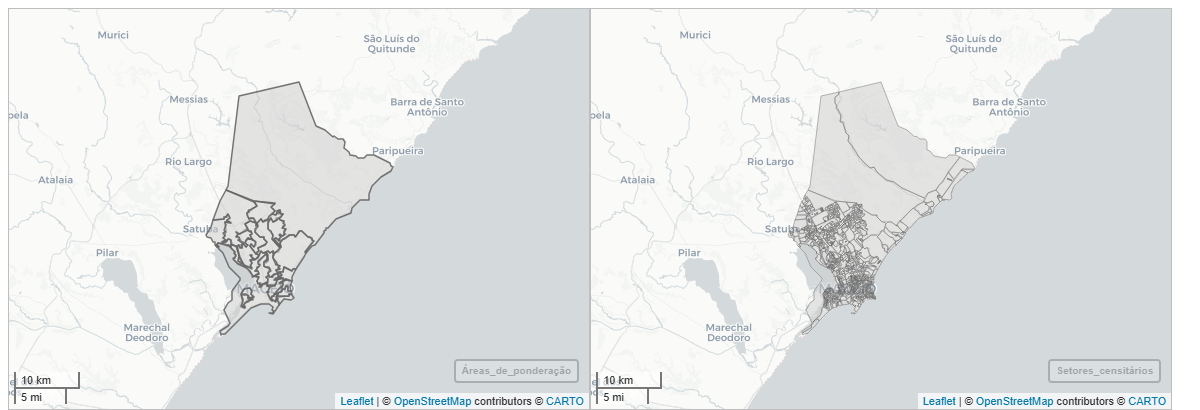
\includegraphics[keepaspectratio]{img/6-conceitos-e-metodos/recortes-intra-institucionais.png}}

}

\end{figure}%

\begin{tcolorbox}[enhanced jigsaw, arc=.35mm, bottomrule=.15mm, bottomtitle=1mm, breakable, colback=white, colbacktitle=quarto-callout-tip-color!10!white, colframe=quarto-callout-tip-color-frame, coltitle=black, left=2mm, leftrule=.75mm, opacityback=0, opacitybacktitle=0.6, rightrule=.15mm, title=\textcolor{quarto-callout-tip-color}{\faLightbulb}\hspace{0.5em}{Dica}, titlerule=0mm, toprule=.15mm, toptitle=1mm]

Aproxime o zoom nos dois mapas e observe os contornos dos polígonos. É
comum perceber pequenas imperfeições nas bordas das feições, com
vértices deslocados. Isso ocorre porque o parâmetro
\texttt{simplified\ =\ TRUE} é o padrão em todas as funções do
\texttt{geobr}, o que reduz o tamanho dos arquivos e acelera o
processamento, ao custo de simplificar a geometria. Para reproduzir os
mapas com geometrias precisas, execute o código localmente com
\texttt{simplified\ =\ FALSE} nos dois downloads e aproxime o zoom
novamente para verificar como as bordas ficam com os contornos
regularizados.

\end{tcolorbox}

\section{Principais aspectos
metodológicos}\label{principais-aspectos-metodoluxf3gicos}

Entendido o papel do IBGE e os seus principais recortes geográficos,
podemos voltar ao foco do nosso capítulo. O Censo Demográfico é o maior
e mais complexo levantamento estatístico do Brasil. Diferente das
pesquisas por amostragem (como a PNAD-C, a POF ou a PNS, que entrevistam
apenas uma fração dos domicílios), o Censo tem como ambição cobrir todos
os domicílios do território nacional, sem exceção. Essa universalidade é
o que o torna insubstituível, pois é a única pesquisa capaz de fornecer
informações estatísticas desagregadas em qualquer recorte do território,
desde o nível nacional até o setor censitário.

Os dois objetivos principais do Censo são contar todos os habitantes do
território nacional e identificar as condições em que vivem. O primeiro
recenseamento do território brasileiro foi realizado em 1872, no Período
Imperial. A partir de 1890, o Censo passou a ter periodicidade decenal,
sendo esta frequência formalmente estabelecida pela Lei nº 8.184/1991
(Brasil, 1991). No século XX, embora as edições previstas para 1910 e
1930 não tenham sido realizadas, os Censos de 1940, 1950, 1960, 1970,
1980 e 1991 foram realizados com sucesso. Já no século XXI, tivemos as
edições de 2000, 2010 e 2022. Este último intervalo maior de 12 anos
ocorreu em razão e de dificuldades no planejamento e financiamento da
pesquisa, agravadas ainda pela pandemia da COVID-19, o que inviabilizou
sua realização no ano previsto de 2020.

\begin{tcolorbox}[enhanced jigsaw, arc=.35mm, bottomrule=.15mm, bottomtitle=1mm, breakable, colback=white, colbacktitle=quarto-callout-note-color!10!white, colframe=quarto-callout-note-color-frame, coltitle=black, left=2mm, leftrule=.75mm, opacityback=0, opacitybacktitle=0.6, rightrule=.15mm, title=\textcolor{quarto-callout-note-color}{\faInfo}\hspace{0.5em}{Nota}, titlerule=0mm, toprule=.15mm, toptitle=1mm]

\textbf{Desafios do Censo de 2022}

A coleta do Censo Demográfico 2022 começou em 1º de agosto de 2022 e foi
concluída em 28 de maio de 2023. Em outubro de 2022, prazo inicialmente
previsto para o encerramento da operação, haviam sido recenseadas 70\%
das pessoas de 14 anos ou mais que seriam efetivamente investigadas até
o fim da coleta. Em fevereiro de 2023, esse percentual chegou a 96,4\%
e, em março, a 97,8\%. Para comparação, no Censo 2010 o patamar de 97\%
já havia sido alcançado em outubro de 2010, dentro do prazo tradicional
de três meses. O desempenho mais baixo do Censo 2022 até outubro
decorreu de diversos fatores, entre eles dificuldades de contratação de
pessoal pelo IBGE e a menor disposição da população em responder ao
recenseamento. Esse declínio nas taxas de resposta em pesquisas e censos
com entrevistas diretas, contudo, não é um fenômeno exclusivo do Brasil,
tendo sido registrado também em outros países.

\end{tcolorbox}

Realizar um censo demográfico é uma das operações logísticas mais
complexas que um Estado pode empreender. Para o
\href{https://censo2022.ibge.gov.br/sobre/geografia-censitaria/base-territorial.html}{Censo
de 2022}, o IBGE coordenou 183 mil agentes recenseadores distribuídos em
468 mil setores censitários de todos os municípios do país. Com a missão
de visitar individualmente cada domicílio brasileiro, incluindo áreas
urbanas densas, zonas rurais isoladas, territórios indígenas e
comunidades de difícil acesso, estes agentes percorreram mais de
\href{https://agenciadenoticias.ibge.gov.br/agencia-noticias/2012-agencia-de-noticias/noticias/41911-censo-2022-na-casa-brasil-ibge-equipe-tecnica-divulga-os-agregados-por-setores-censitarios-e-trajetos-dos-recenseadores}{13,4
milhões de km no território}\footnote{isso equivale a, aproximadamente,
  335 voltas em torno da Terra!}. Essa escala exige anos de preparação
antes do trabalho de campo e anos de processamento e divulgação de
resultados após sua conclusão.

A importância do Censo ultrapassa sua própria produção de dados. Por
oferecer a única contagem exaustiva da população em nível intraurbano,
ele fundamenta o funcionamento de todo o sistema de estatísticas
nacionais. As pesquisas por amostragem do IBGE utilizam os resultados do
Censo para calibrar os pesos de suas amostras, garantindo que os
resultados sejam representativos para a população como um todo.
Projeções populacionais para os anos entre censos, utilizadas para o
planejamento público e a distribuição de recursos entre municípios,
também são calculadas com base nas tendências observadas entre edições
censitárias. Sem o Censo, o sistema estatístico brasileiro perderia sua
referência de ancoragem.

Vale ainda salientar que a metodologia censitária no Brasil é
desenvolvida em diálogo com padrões internacionais. A realização de
censos demográficos periódicos é prática comum entre os institutos
nacionais de estatística ao redor do mundo. Nos Estados Unidos, o
\emph{Census Bureau} conduz um censo decenal desde 1790, complementado
pela \emph{American Community Survey} (ACS), pesquisa amostral anual que
fornece estimativas de características socioeconômicas em nível local
entre os censos. Em Portugal e Espanha, o Instituto Nacional de
Estatística (INE) realiza recenseamentos decenais com estrutura
metodológica semelhante à do IBGE. O \emph{Statistics Canada} conduz o
censo a cada cinco anos, alternando entre um recenseamento completo e
uma versão com questionário expandido aplicado a uma amostra.

Todos estes institutos possuem como referência global o documento
\emph{Principles and Recommendations for Population and Housing
Censuses} (United Nations Statistics Division, 2025), publicado pela
Divisão de Estatística das Nações Unidas (UNSD, Série M67). A versão
mais recente, a Revisão 4 do documento, aprovada pela Comissão de
Estatística da ONU em março de 2025, orienta o chamado \emph{Census
Round} 2030, o ciclo internacional de censos que abrange os
recenseamentos realizados ao longo da década de 2030.

Para coordenar a produção dessa revisão, a ONU organizou grupos de
trabalho temáticos, os \emph{Task Teams}. O IBGE preside o \textbf{Task
Team 3: Use of Geospatial Information in Census Operations}, responsável
por consolidar as recomendações sobre o uso de informação geoespacial
nas operações censitárias.\footnote{A atuação do IBGE nesses fóruns é
  antiga. Desde 1950, os recenseamentos gerais brasileiros foram
  realizados de forma integrada ao Censo das Américas, programa
  continental de uniformização de conceitos e comparabilidade de
  resultados patrocinado pelo Instituto Interamericano de Estatística a
  pedido da ONU, arranjo que se repetiu nas edições de 1960, 1970 e 1980
  (Instituto Brasileiro de Geografia e Estatística, s. d.). O Brasil já
  figurava entre os países-membros da Comissão de Estatística das Nações
  Unidas em 1974 (United Nations Statistical Commission, 1974) e ocupou
  assentos em seu \emph{Bureau} em diferentes momentos, representado por
  presidentes do instituto, com Isaac Kerstenetzky na 20ª sessão (1979),
  Jessé de Souza Montello na 23ª (1985) e Eduardo Augusto Guimarães na
  26ª (1991) (United Nations Statistics Division, s. d.). Em 2016 e
  2017, Wasmália Bivar presidiu a Comissão e conduziu o acordo global
  sobre o quadro de indicadores dos Objetivos de Desenvolvimento
  Sustentável (United Nations Statistics Division, 2017).} O Task Team 3
conta com a participação de institutos e organismos de vários países e
regiões, entre eles Indonésia, Austrália, Colômbia, Índia, Quênia e
Polônia, além de organizações como a Comissão Europeia (Eurostat), o
Banco Mundial, a CEPAL e o UNFPA. A presidência brasileira desse grupo
reflete o reconhecimento internacional do trabalho do IBGE na integração
entre estatística e geografia na condução de pesquisas deste porte.

\begin{tcolorbox}[enhanced jigsaw, arc=.35mm, bottomrule=.15mm, bottomtitle=1mm, breakable, colback=white, colbacktitle=quarto-callout-note-color!10!white, colframe=quarto-callout-note-color-frame, coltitle=black, left=2mm, leftrule=.75mm, opacityback=0, opacitybacktitle=0.6, rightrule=.15mm, title=\textcolor{quarto-callout-note-color}{\faInfo}\hspace{0.5em}{Nota}, titlerule=0mm, toprule=.15mm, toptitle=1mm]

\textbf{Desafios e limitações do Censo}

A realização de um censo demográfico envolve desafios logísticos e
metodológicos consideráveis. Um dos principais é a impossibilidade de
garantir cobertura total da população. Nas operações censitárias, dois
tipos de erro de cobertura podem ocorrer. A \emph{omissão} acontece
quando pessoas que deveriam ter sido recenseadas não foram e a
\emph{inclusão indevida} quando pessoas são contadas quando não deveriam
ter sido. A diferença entre ambos é chamada de \emph{erro líquido de
enumeração}, a medida mais usada para avaliar a qualidade da cobertura.

Para o Censo de 2022, a Pesquisa de Pós-Enumeração (PPE) (IBGE, 2024d)
estimou um erro líquido de enumeração de \textbf{8,3\%} da população
recenseada, composto por uma taxa de omissão de \textbf{12,2\%} e de
inclusão indevida de \textbf{3,3\%}. Esses erros não se distribuem
uniformemente pelo território. O Rio de Janeiro registrou a maior taxa
entre os estados (15,5\%), seguido por Rondônia (11,2\%), Roraima
(10,9\%), Amapá (10,8\%) e São Paulo (10,8\%). No extremo oposto,
Paraíba (3,8\%), Piauí (4,1\%) e Alagoas (4,8\%) apresentaram as menores
taxas. As regiões Sul e Nordeste ficaram inteiramente abaixo da média
nacional, enquanto estados do Norte e do Sudeste tiveram desempenho
pior. Há também uma relação clara com o porte dos municípios, onde
municípios com menos de 14.000 habitantes registraram erro líquido de
3,9\%, enquanto municípios com mais de um milhão de habitantes chegaram
a 13,2\%. Nas grandes cidades, contribuem para esse resultado o difícil
acesso a condomínios fechados e as adversidades da coleta em favelas e
comunidades urbanas, onde o endereçamento precário e problemas de
segurança pública limitam a atuação dos recenseadores.

Outro aspecto metodológico relevante para a interpretação dos dados é a
\emph{imputação}. Quando um domicílio é classificado como ocupado, mas a
entrevista não é realizada (por recusa, ausência dos moradores ou
dificuldade de acesso), o IBGE não o registra automaticamente como dado
faltante/ausente. Em vez disso, atribui-se a ele o número de moradores
de um domicílio com perfil semelhante (o chamado domicílio
\emph{doador}), selecionado com base na situação do setor (urbano ou
rural), no porte do município, no tipo de espécie do domicílio e na
classe socioeconômica do setor censitário. No Censo de 2022, foram
imputadas aproximadamente \textbf{8 milhões de pessoas} (3,9\% do total
de 203 milhões), com São Paulo registrando a maior taxa estadual
(7,7\%).

Por fim, a periodicidade decenal representa uma limitação estrutural.
Com intervalos de dez anos entre censos, os dados envelhecem rapidamente
em um país com dinâmica urbana acelerada. Para mitigar essa limitação, o
IBGE realiza periodicamente pesquisas amostrais que permitem atualizar
estimativas entre censos, mas sem a mesma granularidade espacial.

\end{tcolorbox}

A partir dessa compreensão introdutória, podemos então apresentar os
principais métodos de coleta desta pesquisa e seus respectivos produtos,
cujo conteúdo será explorado de forma mais detalhada nos próximos
capítulos.

\subsection{Os Instrumentos de Coleta do
Censo}\label{os-instrumentos-de-coleta-do-censo}

O \textbf{setor censitário} é a menor porção territorial em que o Brasil
é dividido para fins de coleta estatística. Trata-se de uma área
contínua cujo dimensionamento leva em conta a extensão geográfica e a
quantidade de domicílios ou estabelecimentos agropecuários nela
presentes (IBGE, 2022b). Nas áreas urbanas, os setores tendem a ser
menores e mais densamente ocupados. Nas rurais, abrangem extensões
maiores com população dispersa. Conforme mencionado anteriormente, para
o Censo de 2022, o território brasileiro foi dividido em \textbf{468 mil
setores censitários}, quase 158 mil a mais que os 310 mil setores da
edição de 2010.

De acordo com o Manual do Recenseador (IBGE, 2022a), cada setor
censitário é de responsabilidade de um único recenseador, apesar de
haver exceções como as coletas por \textbf{mutirão}\footnote{Ocorrem,
  geralmente, em setores unidades recenseáveis muito acima da média (300
  domicílios), com objetivo de ganhos de eficiência na coleta em função
  grande extensão territorial e questões de segurança. Porém, devem ser
  a exceção e não a regra.}. Dentro de cada setor, a operação de campo
segue uma sequência com duas fases principais. Na primeira, denominada
pelo IBGE \textbf{etapa de reconhecimento do setor censitário}, os
Agentes Censitários Supervisores (ACS) percorrem as faces de quadra para
coletar informações sobre a infraestrutura do entorno e atualizar o mapa
do setor, identificando logradouros que orientarão o trabalho posterior.

Antes de iniciar a coleta propriamente dita, os próprios recenseadores
também realizam um reconhecimento individual de sua área de trabalho,
analisando o mapa do setor, planejando o percurso e sanando dúvidas de
localização com o ACS responsável (IBGE, 2022a). Somente após essa
preparação tem início a \textbf{coleta domiciliar}, em que os
recenseadores percorrem os endereços do setor, aplicam os questionários
e registram as coordenadas geográficas e a espécie de cada localização
visitada. Essa sequência organiza o conjunto de instrumentos de coleta
do Censo, cada um com finalidade, cobertura e método próprios, cujos
detalhese são melhor especificados a seguir.

\subsubsection{Questionário da Pesquisa Urbanística do Entorno dos
Domicílios}\label{questionuxe1rio-da-pesquisa-urbanuxedstica-do-entorno-dos-domicuxedlios}

A Pesquisa Urbanística do Entorno dos Domicílios corresponde à etapa de
reconhecimento do setor descrita anteriormente e tem a finalidade de
coletar dados de infraestrutura urbana e identificar logradouros que
orientarão o trabalho dos recenseadores. É conduzida pelos
\textbf{Agentes Censitários Supervisores (ACS)}, que percorrem as faces
de quadra a pé utilizando o \textbf{DMC} (Dispositivo Móvel de Coleta),
aparelho semelhante a um \emph{smartphone} equipado com o aplicativo de
coleta do IBGE. A pesquisa cobriu cerca de 340 mil dos 468 mil setores
existentes, abrangendo os setores urbanos faceados\footnote{Um setor
  \textbf{faceado} é aquele cujos limites são definidos por faces de
  quadra, ou seja, os trechos de logradouro entre duas esquinas
  consecutivas, o que permite percorrê-lo sistematicamente pela calçada,
  frente a frente com os imóveis.} e setores rurais com áreas
urbanizadas mapeadas, em todos os 5.568 municípios do país.

Para cada face percorrida, o ACS preenche por observação direta, sem
entrevistar moradores, um questionário padronizado que investiga
aspectos como capacidade de circulação da via\footnote{com relação ao
  tamanho dos veículos que podem trafegar pela mesma}, pavimentação,
bueiros, iluminação pública, pontos de parada de ônibus ou van,
sinalização para bicicletas, existência e condições das calçadas, rampas
para cadeirantes e arborização (IBGE, 2025a).

A coleta pelos ACS ocorreu predominantemente entre 20 de junho e 31 de
julho de 2022, antes do início da coleta domiciliar. Durante as
entrevistas domiciliares, os recenseadores puderam efetuar ajustes nas
informações registradas pelos ACS. As informações do entorno têm como
referência a data efetiva de coleta em campo, diferentemente dos
questionários domiciliares, cujo momento de referência é a meia-noite de
31 de julho para 1º de agosto de 2022. Os dados coletados são publicados
no produto \textbf{Características Urbanísticas do Entorno dos
Domicílios}, descrito na Seção~\ref{sec-produtos_censo}.

\subsubsection{Registro Automático de
Trajeto}\label{registro-automuxe1tico-de-trajeto}

Ao longo de todo o percurso pelo setor, o DMC do recenseador registra
automaticamente e de forma contínua a posição GPS/GNSS, gerando uma
trilha georreferenciada do caminho percorrido. Esse registro automático
permite ao IBGE monitorar a cobertura da coleta em tempo real e
identificar setores com lacunas durante a operação. Os trajetos
registrados são publicados como produto público após o encerramento da
coleta.

\subsubsection{Questionários de entrevista domiciliar (Básico e da
Amostra)}\label{questionuxe1rios-de-entrevista-domiciliar-buxe1sico-e-da-amostra}

Os dois questionários domiciliares do Censo compartilham uma mesma
\textbf{data de referência}, que define quem é recenseável. Para o Censo
de 2022, este momento foi o da meia-noite do dia 31 de julho para 1º de
agosto de 2022\footnote{Pessoas nascidas após esta data não foram
  incluídas no Censo 2022}. Qualquer pessoa que residia em um domicílio
brasileiro nesse momento é, por definição, parte da população
recenseada. Moradores temporariamente ausentes na data da visita do
recenseador são registrados normalmente, desde que o domicílio seja seu
local habitual de residência. Vale salientar que o período de coleta
inicia-se, geralmente, em 31 de agosto e dura aproximadamente 3
meses\footnote{Uma exceção importante foi o Censo de 2022, que só
  concluiu a coleta dos questionários em 28 de maio de 2023, devido a
  dificuldades de contratação de pessoal pelo IBGE e a menor disposição
  da população em responder ao recenseamento}.

Existem dois tipos de questionário aplicados, denominados Questionário
Básico (ou do Universo) e Questionário da Amostra (ou Ampliado). O
\textbf{Questionário Básico} é aplicado em todos os domicílios do país,
exceto naqueles selecionados para a amostra, e investiga as
características fundamentais dos moradores e do domicílio. Este
questionário possuía 34 itens no Censo de 2010, que foram reduzidos para
26 questões no Censo de 2022. Os resultados relativos a esta coleta são
divulgados em forma de agregados (totais, médias e variâncias), no nível
do setor censitário.

Já o \textbf{Questionário da Amostra} é aplicado em uma fração dos
domicílios, selecionados de forma aleatória dentro de cada setor
censitário. Além dos 26 quesitos do Básico, inclui investigações mais
detalhadas sobre temas específicos: identificação étnico-racial,
nupcialidade, núcleo familiar, fecundidade, religião ou culto,
deficiência, migração interna ou internacional, educação, deslocamento
para estudo, trabalho e rendimento, deslocamento para trabalho,
mortalidade e autismo (IBGE, 2024c). No Censo de 2010 o questionário
tinha 102 quesitos e, em 2022, este número foi de 77 (IBGE, 2024a). A
fração amostral varia conforme o porte do município. Nos menores (até
2.500 habitantes) chega a 50\% dos domicílios, ao passo que nos maiores
(acima de 500 mil habitantes) é de apenas 5\%, com média geral de 11\%
(IBGE, 2024c). Os resultados são divulgados por meio de microdados
(respostas individuais), cuja correspondência geográfica ocorre no nível
da \textbf{área de ponderação}, recorte formado por agrupamento de
setores censitários com no mínimo 400 domicílios particulares ocupados
na amostra, garantindo precisão estatística e preservando o anonimato
dos respondentes.

Os questionários foram coletados predominantemente na modalidade
\textbf{CAPI} (\emph{Computer-Assisted Personal Interviewing}), em que o
recenseador realiza a entrevista presencialmente utilizando o DMC.
Complementarmente, o Censo de 2022 também ofereceu coleta por
\textbf{CATI} (\emph{Computer-Assisted Telephone Interviewing}),
entrevista conduzida por telefone pelos recenseadores com seus próprios
DMCs, e por \textbf{CAWI} (\emph{Computer-Assisted Web Interviewing}),
preenchimento realizado pelo próprio morador via portal do Censo na
internet. A CAPI foi responsável por 98,9\% das entrevistas, enquanto
CATI e CAWI responderam por 0,6\% cada (IBGE, 2024a). O uso da internet
como canal de coleta foi uma inovação introduzida no Censo de 2010,
quando cerca de 45 mil questionários foram preenchidos pelos próprios
moradores pelo portal do IBGE, o que correspondeu a aproximadamente
0,07\% dos domicílios visitados (IBGE, 2016b). Vale salientar que a
coleta por telefone (CATI) foi realizada pela primeira vez neste Censo
de 2022.

\subsubsection{Cadastro de Endereços}\label{cadastro-de-endereuxe7os}

Enquanto os questionários coletam informações sobre quem mora nos
domicílios, o cadastro de endereços registra onde esses domicílios
estão. Durante a coleta domiciliar, ao percorrer cada endereço do setor,
o recenseador utiliza o receptor GPS/GNSS integrado ao DMC para capturar
as coordenadas geográficas de cada localização, além de informações
sobre a espécie do endereço (domicílio particular, estabelecimento de
saúde, de ensino, entre outros) e outras características do logradouro.
Antes da operação censitária, o IBGE também atualiza o cadastro de
endereços por outras duas vias, seja incorporando registros
administrativos (como os endereços do Cadastro de Pessoas Físicas) ou em
visitas de campo realizadas por equipes específicas de atualização
(IBGE, 2025a). O conjunto de endereços cadastrados é publicado no
\textbf{Cadastro Nacional de Endereços para Fins Estatísticos (CNEFE)},
produto descrito na seção seguinte.

\subsection{Os produtos do censo}\label{sec-produtos_censo}

O Censo Demográfico produz um conjunto diversificado de produtos de
dados a partir dos instrumentos de coleta apresentados anteriormente,
cada um com características distintas de resolução espacial, riqueza
temática e forma de acesso. Os principais são:

\begin{itemize}
\tightlist
\item
  \textbf{Agregados por setor censitário:} estatísticas (totais, médias
  e variâncias) tabuladas para cada um dos 468 mil setores censitários
  do país, a partir das respostas do Questionário Básico (universo).
  Cobrem características dos domicílios e dos moradores, e incluem
  também variáveis da Pesquisa Urbanística do Entorno dos Domicílios
  agregadas ao nível do setor.
\item
  \textbf{Microdados da Amostra:} registros individuais anonimizados de
  domicílios e moradores que responderam ao Questionário da Amostra,
  identificados até o nível da área de ponderação. Permitem análises
  complexas com controle de variáveis socioeconômicas.
\item
  \textbf{Grade Estatística:} contagens populacionais e de domicílios
  distribuídas em células regulares de 200 × 200 m nas áreas urbanas e 1
  × 1 km nas rurais, oferecendo a maior resolução espacial dos produtos
  do Censo.
\item
  \textbf{Cadastro Nacional de Endereços para Fins Estatísticos
  (CNEFE):} cadastro georreferenciado de todos os endereços visitados
  durante a operação censitária, com coordenadas geográficas e
  informações sobre a espécie de cada localização. No Censo de 2022
  foram cadastrados 106,8 milhões de endereços (IBGE, 2024b).
\item
  \textbf{Características Urbanísticas do Entorno dos Domicílios:}
  informações sobre a infraestrutura urbana coletadas na Pesquisa
  Urbanística do Entorno dos Domicílios. Embora a unidade de coleta seja
  a face de quadra, a melhor resolução espacial disponível ocorre no
  nível do \textbf{setor censitário} (estatísticas de totais e
  percentuais), com possibilidade de agregação também por
  \textbf{bairro, subdistrito, distrito e município} (IBGE, 2025a).
\item
  \textbf{Trajeto dos Recenseadores:} dados georreferenciados das
  trilhas percorridas por todos os recenseadores durante a operação de
  campo, disponibilizado publicamente pelo IBGE após o encerramento da
  coleta.
\item
  \textbf{Produtos temáticos:} o Censo produz ainda resultados
  específicos para territórios indígenas, comunidades quilombolas e
  favelas e comunidades urbanas.
\end{itemize}

Antes de fecharmos este capítulo, é importante compreender uma
característica marcante que orienta o uso desses produtos. Diz respeito
à relação inversa entre resolução espacial e riqueza temática das
informações divulgadas. Quanto maior a resolução espacial, menor a
quantidade de estatísticas disponíveis naquele nível. Isso decorre em
larga medida pela obrigação do IBGE em garantir o sigilo das informações
individuais coletadas. Em unidades geográficas muito pequenas, divulgar
muitas variáveis aumenta o risco de que uma combinação de
características permita identificar um domicílio ou uma pessoa
específica. Por essa razão, a grade estatística (a maior resolução
espacial) disponibiliza apenas totais populacionais e de domicílios,
enquanto os microdados do Questionário da Amostra, muito mais ricos
tematicamente, são identificados apenas até o nível da área de
ponderação. A Figura~\ref{fig-res-esp-vol-est} ilustra esse
\emph{trade-off} utilizando mapas de diferentes recortes geográficos
para o município de Salvador. Observe que à medida que a resolução
espacial aumenta, o volume de estatísticas disponíveis (oriunda dos seus
produtos correspondentes) diminui.

\begin{figure}[H]

\caption{\label{fig-res-esp-vol-est}Relação entre resolução espacial e
volume de estatísticas nos produtos do Censo Demográfico.}

\centering{

\pandocbounded{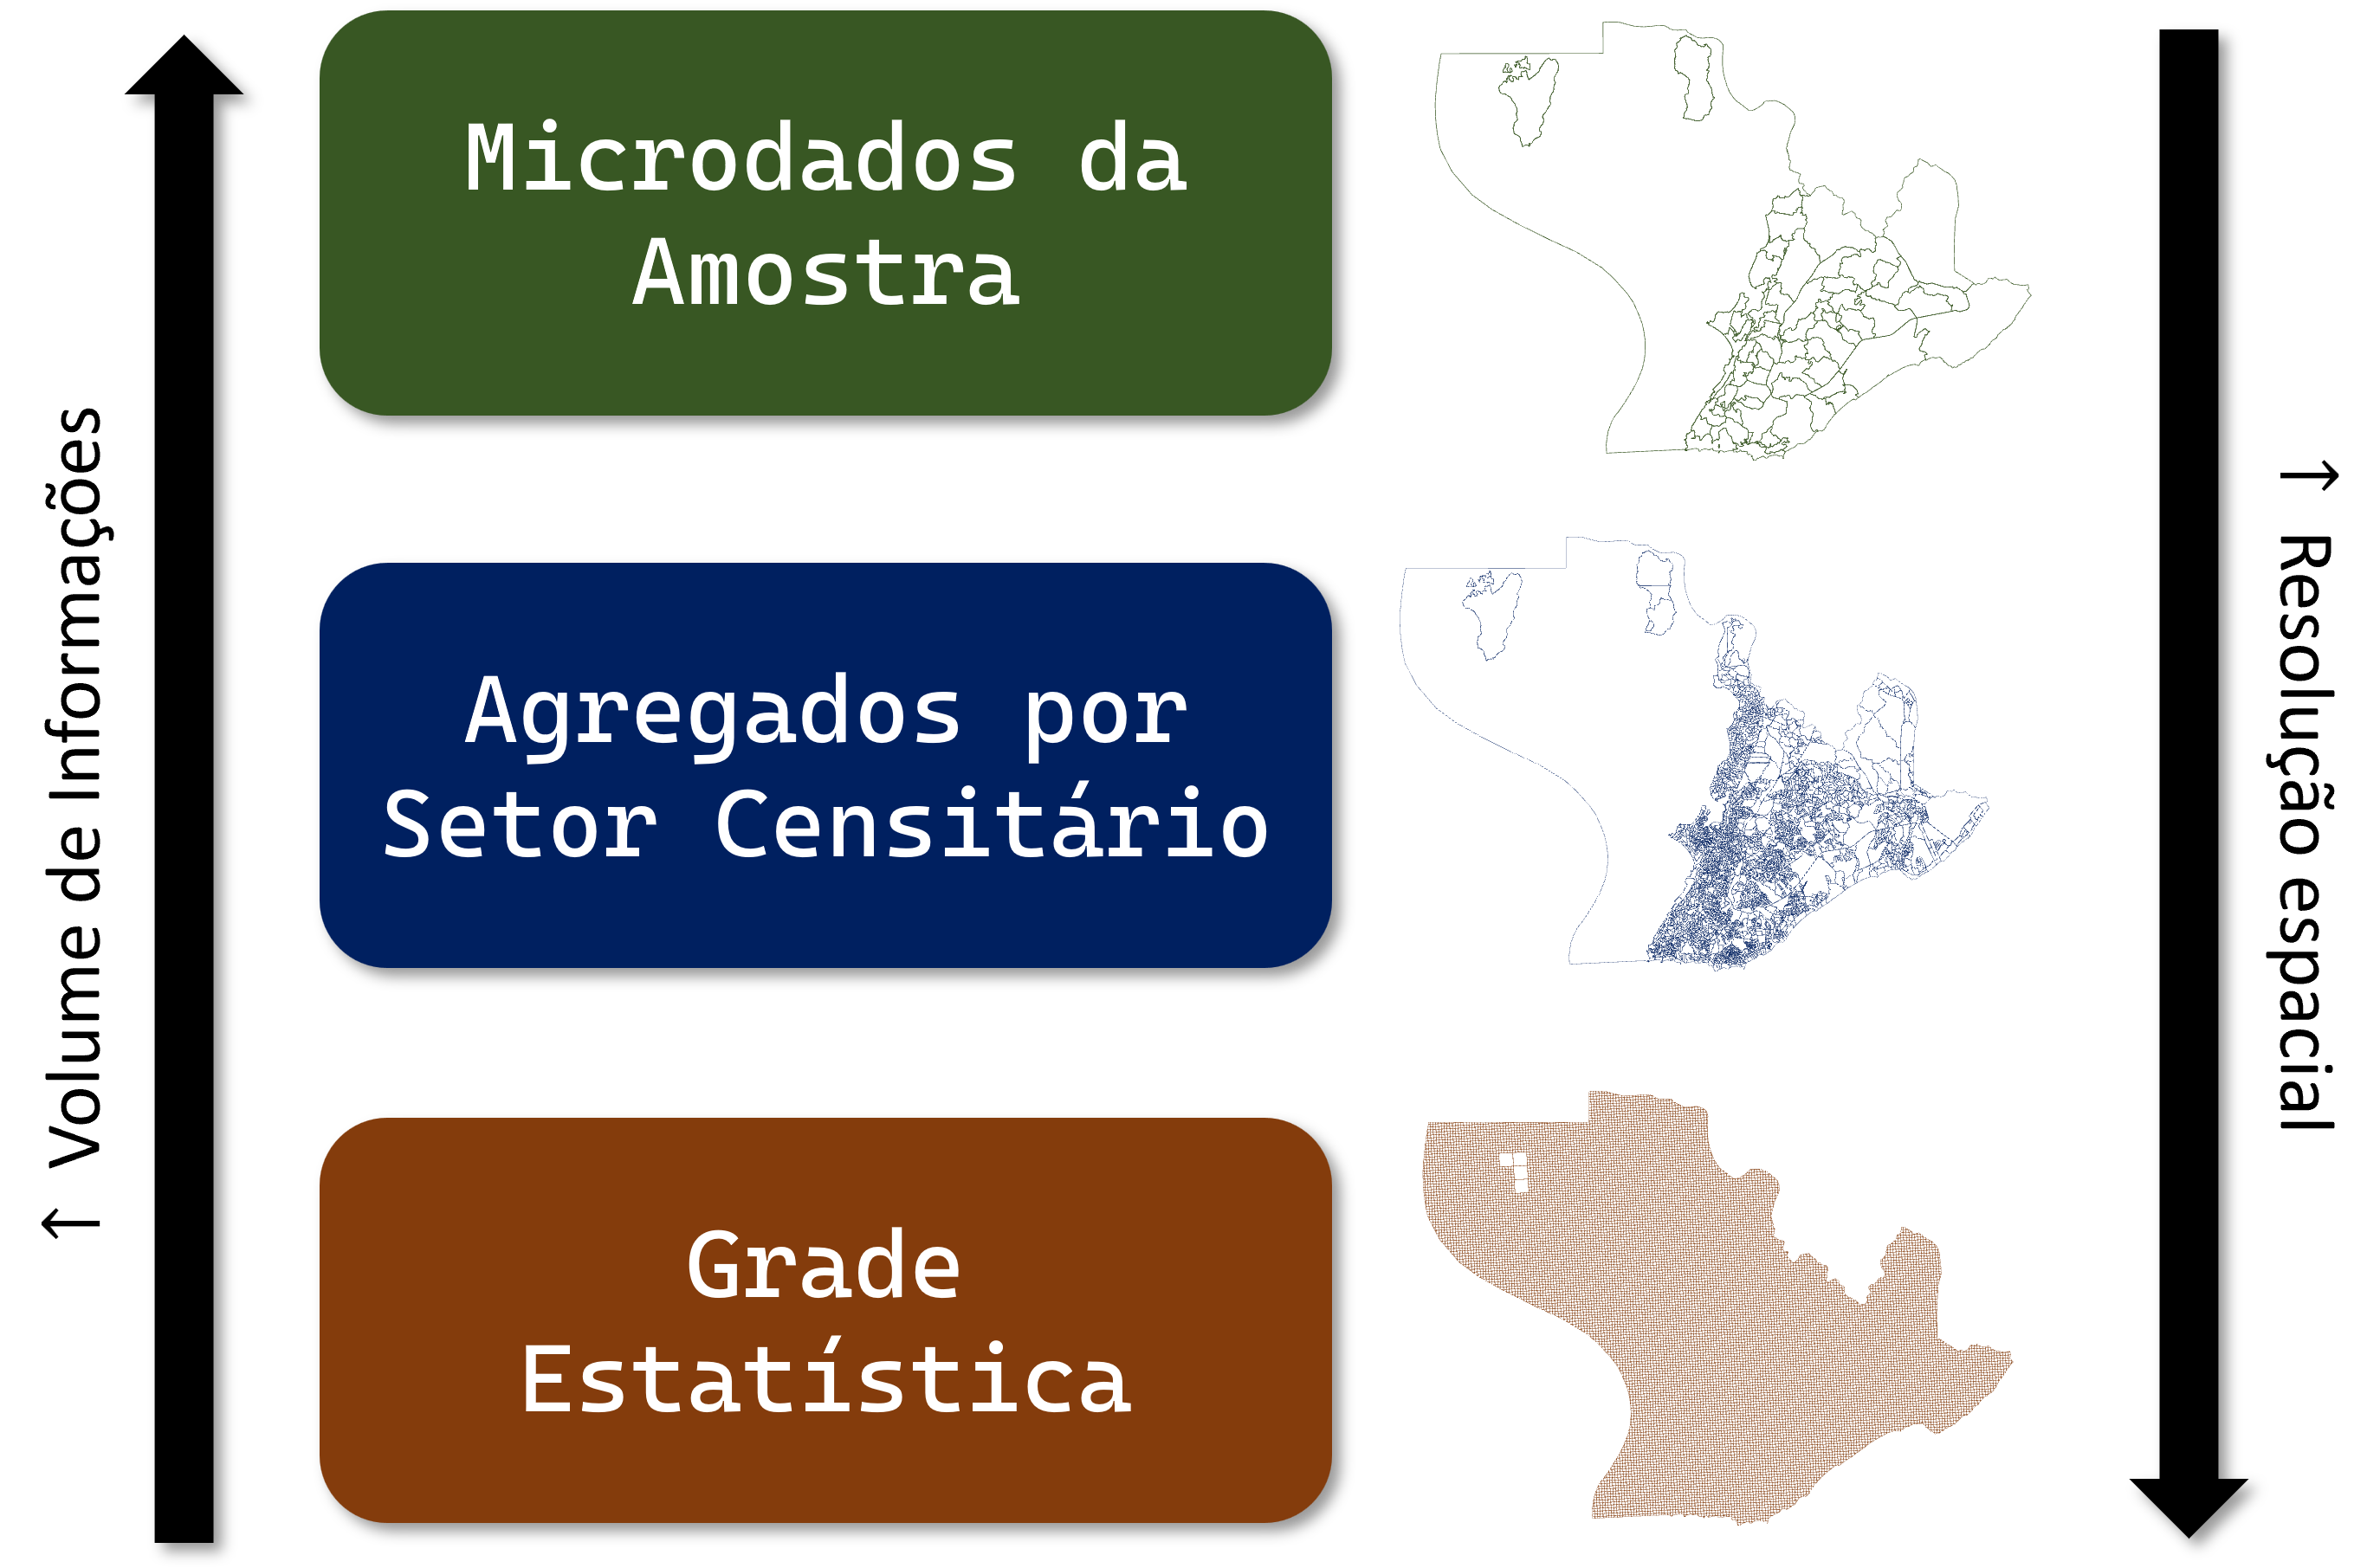
\includegraphics[keepaspectratio]{img/6-conceitos-e-metodos/res_esp_vs_vol_est.png}}

}

\end{figure}%

\chapter{Agregados por Setor
Censitário}\label{agregados-por-setor-censituxe1rio}

\section{Introdução}\label{introduuxe7uxe3o-1}

O produto \textbf{Agregados por Setores Censitários} é um dos resultados
do Censo mais amplamente utilizados por pesquisadores, planejadores e
gestores públicos. Trata-se de um conjunto de tabelas em que cada linha
representa um setor censitário e cada coluna representa uma variável
agregada, como o total de moradores, o número de domicílios, as
condições de abastecimento de água e esgotamento sanitário e a
composição etária da população.

A popularidade desse produto decorre do equilíbrio entre resolução
espacial e quantidade de estatísticas disponível por unidade espacial.
Enquanto os microdados da amostra permitem análises mais ricas em termos
de variáveis (renda, educação, migração), as \textbf{áreas de
ponderação} (unidade espacial dos microdados) são muito maiores que os
setores censitários. Para se ter uma ideia, no Censo de 2010, o
município de São Paulo possuía 5.082 setores censitários, mas apenas 107
áreas de ponderação, conforme ilustra a Figura~\ref{fig-sp-comparacao}.
A grade estatística, por sua vez, oferece resolução ainda maior com as
quadrículas urbanas de 200 x 200 m, mas contém somente totais de
população e domicílio.

\begin{figure}[H]

\caption{\label{fig-sp-comparacao}Setores censitários e áreas de
ponderação do município de São Paulo (Censo 2010).}

\begin{minipage}[t]{0.50\linewidth}

\subcaption{\label{fig-sp-comparacao-1}5.082 setores censitários}

\centering{

\pandocbounded{
\includegraphics[keepaspectratio]{7-agregados_files/figure-pdf/fig-sp-comparacao-1.pdf}}

}

\end{minipage}%
%
\begin{minipage}[t]{0.50\linewidth}

\subcaption{\label{fig-sp-comparacao-2}107 áreas de ponderação}

\centering{

\pandocbounded{
\includegraphics[keepaspectratio]{7-agregados_files/figure-pdf/fig-sp-comparacao-2.pdf}}

}

\end{minipage}%

\end{figure}%

O produto que conhecemos hoje tem uma origem mais modesta do que a
dimensão atual sugere. A ideia de setor censitário, como a menor unidade
espacial de trabalho do Censo, só veio surgir
\href{https://www.ibge.gov.br/estatisticas/sociais/saude/9662-censo-demografico-2010.html?edicao=9754&t=conceitos-e-metodos}{pela
primeira vez no Censo de 1950}. Antes do Censo 1991, esses arquivos eram
concebidos como cadastros de apoio às operações internas do IBGE, com a
finalidade de viabilizar a seleção de amostras em pesquisas domiciliares
posteriores (IBGE, 2024a). Para isso, era suficiente registrar variáveis
descritivas da divisão territorial e informações sobre o porte dos
setores, como o total de domicílios e estimativas de variância que
orientavam a determinação do tamanho das amostras.

No Censo 2000, o IBGE produziu a primeira edição dos agregados por setor
censitário, reunindo 527 variáveis sobre características dos domicílios,
dos responsáveis e das pessoas residentes, com cruzamentos
exclusivamente por sexo. Uma segunda edição, gerada a partir dos
microdados do universo, expandiu esse conjunto para mais de 3200
variáveis, organizadas em planilhas separadas por Unidade da Federação.

No Censo 2010, houve uma consolidação deste produto, com divulgação não
só no nível dos setores, mas também em Grandes Regiões, Unidades da
Federação, Municípios, Distritos, Subdistritos, Bairros e Regiões
Metropolitanas (IBGE, 2016b). Nesta edição, houve o acréscimo de
variáveis relativas a rendimento, tipologia do setor censitário e
características do entorno dos domicílios urbanos, totalizando cerca de
3000 variáveis.

No Censo 2022, os arquivos cobrem, pela primeira vez, dados sobre povos
indígenas e quilombolas em nível de setor, além dos temas já
consolidados de domicílios, demografia, alfabetização, cor ou raça,
mortalidade e relações de parentesco, com mais de 3500 variáveis
distribuídas em diversos arquivos temáticos (IBGE, 2024a). Não obstante,
com a redução do questionário Básico (de 34, em 2010, para 26, em 2022),
houve perda de variáveis importantes como o rendimento de todos os
membros do domicílio.

Antes de partirmos para a exploração destes dados, vamos entender
primeiramente alguns conceitos importantes que norteiam o levantamento e
a organização destes dados, sobretudo aqueles referentes a
\textbf{moradores} e aos tipos de \textbf{domicílio}.

\section{Conceitos importantes}\label{conceitos-importantes}

Para usar corretamente os dados dos agregados, é essencial compreender
como o IBGE conceitua moradores e classifica os domicílios. Muitas das
variáveis disponíveis nos arquivos temáticos dizem respeito a categorias
específicas dessa classificação (como domicílios particulares
permanentes ocupados ou domicílios coletivos com morador) e seu
significado só fica claro a partir desse sistema conceitual.

O ponto de partida é a definição de \textbf{morador(a)}. Para o Censo de
2022, é a pessoa que residia no domicílio na data de referência, ou
seja, à meia-noite da transição do dia 31 de julho ao dia 1º de agosto
de 2022. Mais especificamente, refere-se a alguém que tem aquele
domicílio como local habitual de residência e se encontrava presente no
mesmo na data de referência. Todavia, há pessoas que possuem um certo
domicílio como local habitual de residência, mas estavam ausentes no
período de referência. Nestes casos, esta pessoa ainda é considerada
moradora daquele local, caso essa ausência seja inferior a 12 meses e
tenha ocorrido por um dos seguintes motivos (IBGE, 2016b): viagens (a
passeio, serviço, negócio, estudos, etc.); internação em estabelecimento
de ensino ou hospedagem em outro domicílio, pensionato, república de
estudantes (visando facilitar a frequência durante o ano letivo);
detenção, sem sentença definitiva declarada; internação temporária em
hospital ou estabelecimento similar; ou embarque a serviço (militares,
petroleiros, etc.).

Já o conceito de domicílio refere-se a todo local estruturalmente
\textbf{separado} e \textbf{independente} que serve de habitação a uma
ou mais pessoas. Os critérios de separação (limitado por paredes, muros
ou cercas, com cobertura) e de independência (acesso direto, sem passar
por local de moradia de outras pessoas) devem ser atendidos
simultaneamente para que um espaço seja classificado como domicílio
(IBGE, 2024a).\footnote{Nas áreas indígenas, este conceito é
  flexibilizado para abranger a diversidade de domicílios de grupos
  variados}

A Figura~\ref{fig-domicilios} ilustra a árvore de classificação dos
domicílios adotada pelo IBGE.

\begin{figure}[H]

\caption{\label{fig-domicilios}Classificação dos domicílios no Censo
Demográfico 2022.}

\centering{

\pandocbounded{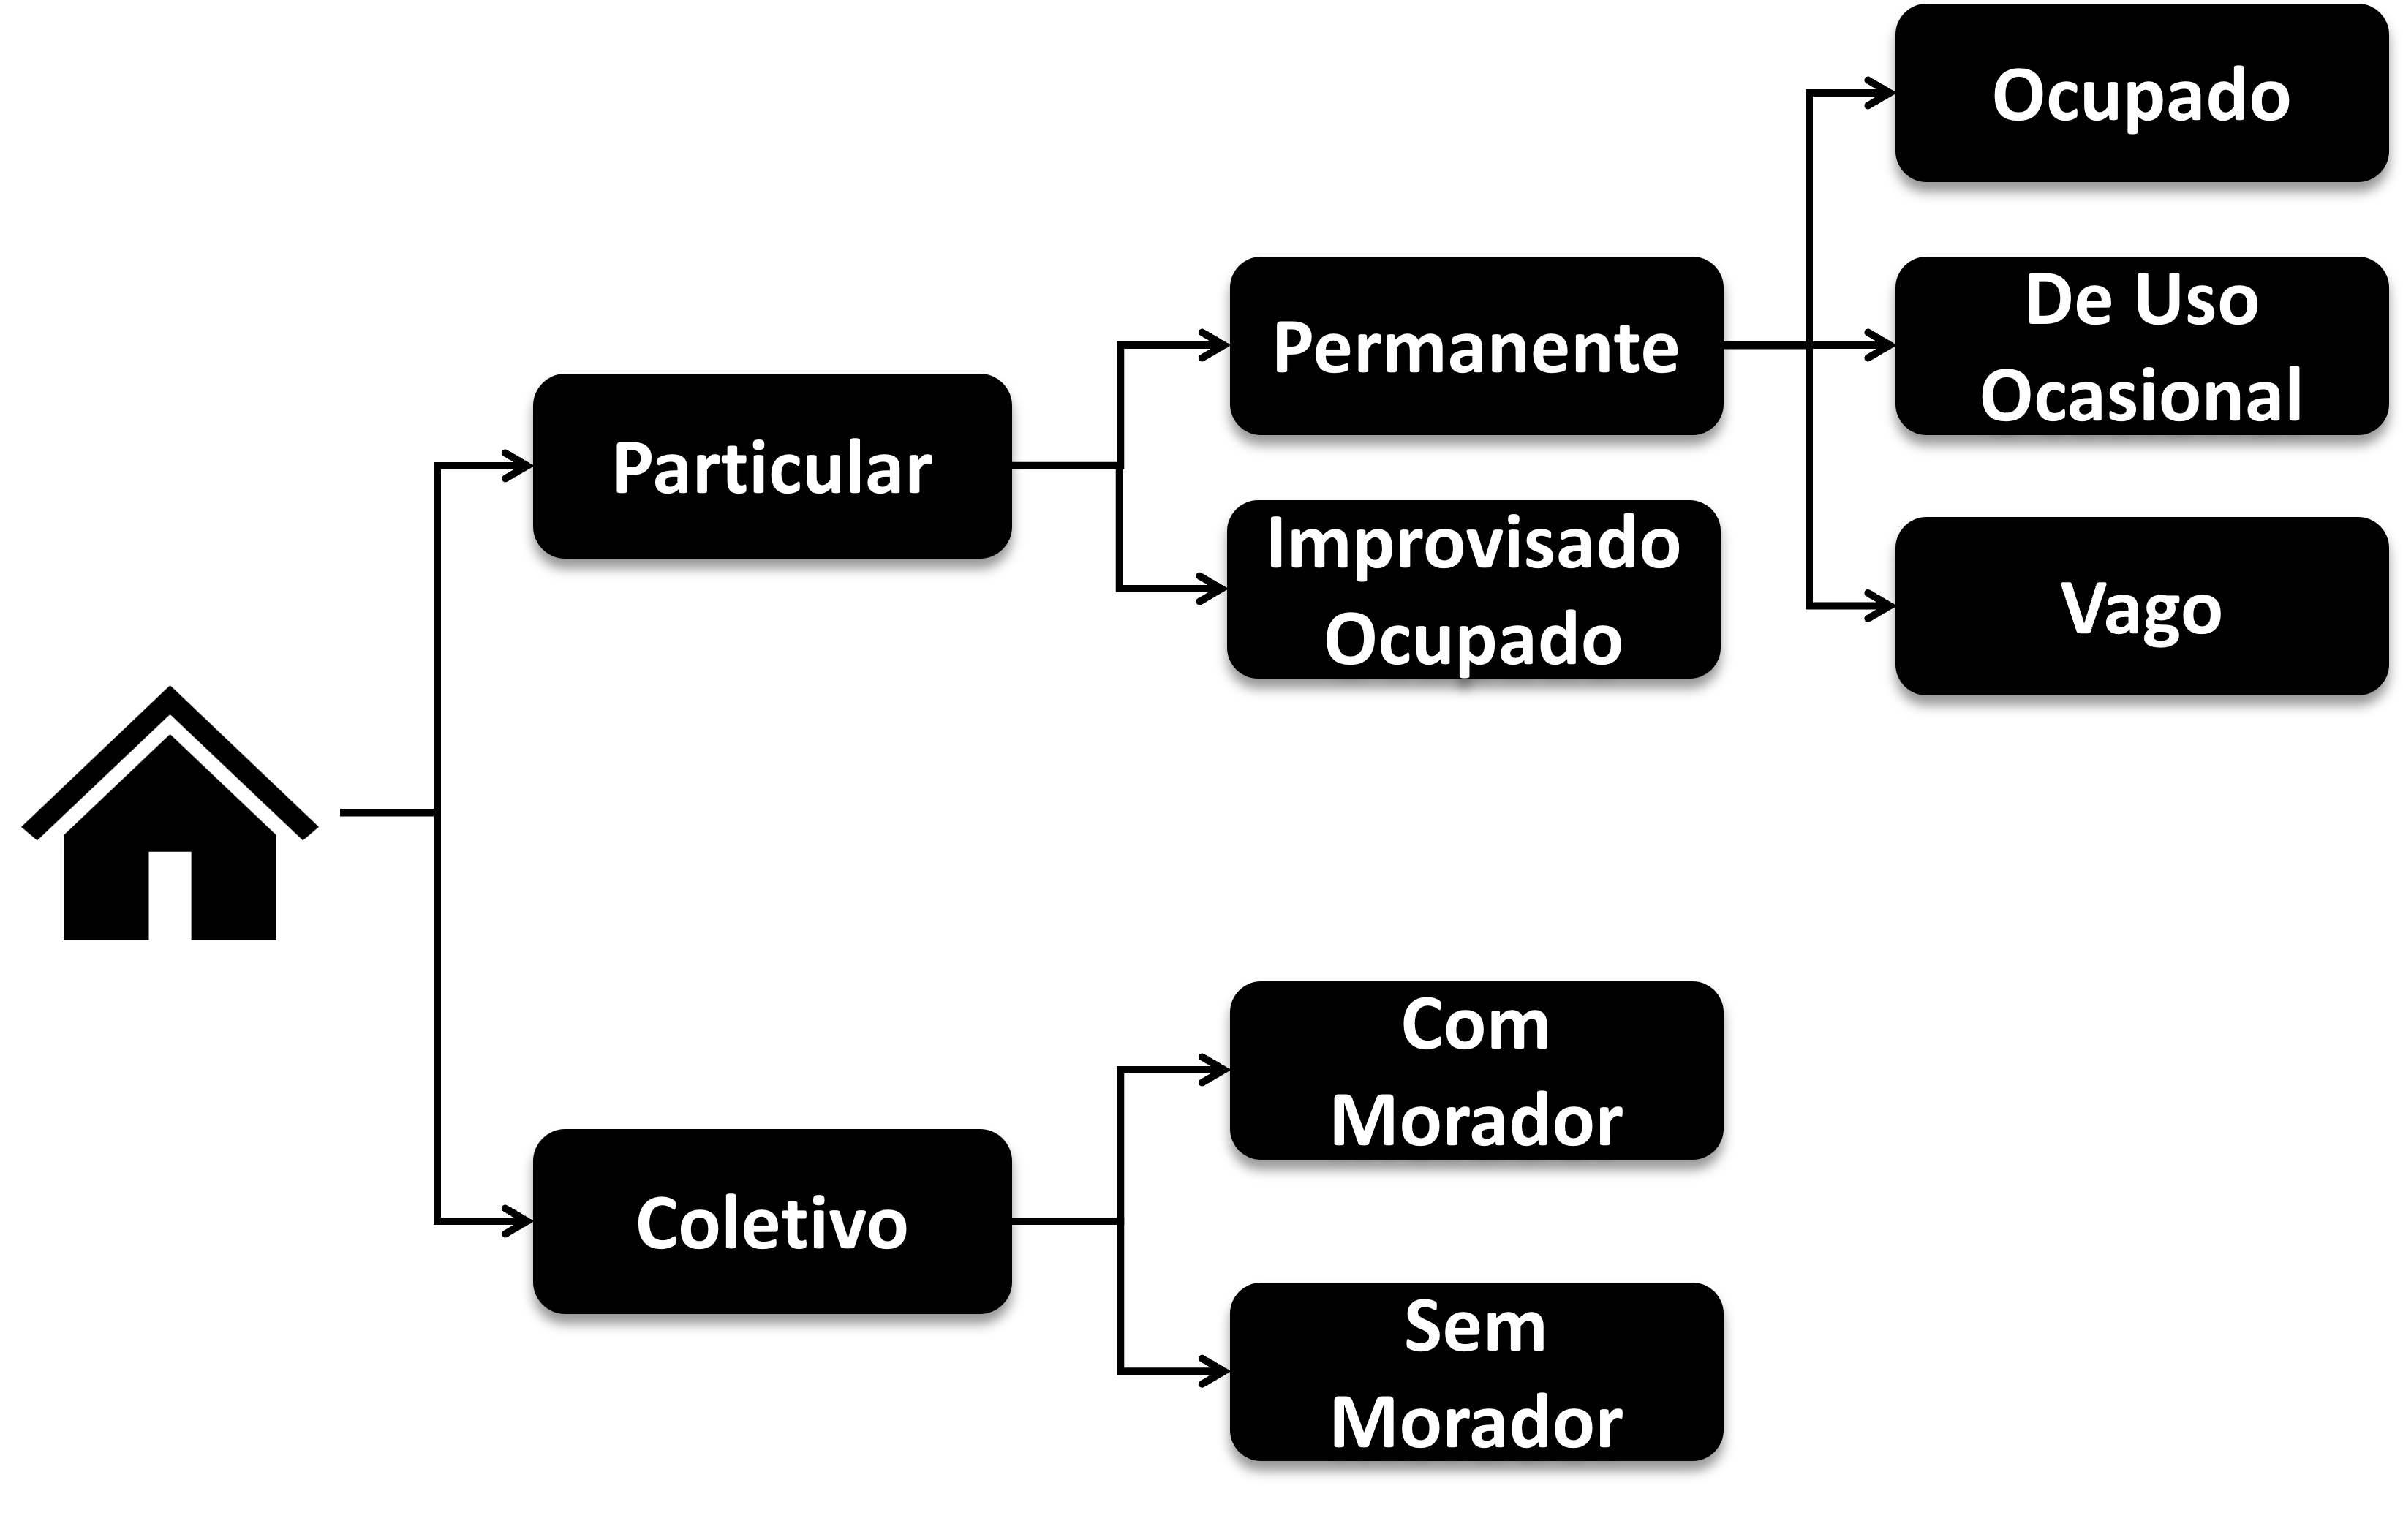
\includegraphics[keepaspectratio]{img/7-agregados/domicilios.png}}

}

\end{figure}%

A divisão principal separa os domicílios em dois grandes grupos:

\textbf{Domicílios particulares} são aqueles em que o relacionamento
entre os ocupantes é ditado por laços de parentesco, de dependência
doméstica ou por normas de convivência. Dentro desse grupo, há duas
subcategorias:

\begin{itemize}
\tightlist
\item
  \emph{Permanentes}: construídos com a finalidade exclusiva de servir
  como habitação. São classificados em três subtipos\footnote{pode-se
    considerar ainda a presença de um quarto subtipo \emph{Ocupado sem
    entrevista}, consistindo de domicílio que estava habitado na data de
    referência, mas os moradores estavam ausentes ou se recusaram a
    responder. Para esses casos, o IBGE aplica imputação estatística com
    base em domicílios semelhantes do mesmo setor}:

  \begin{itemize}
  \tightlist
  \item
    \emph{Ocupado}: estava habitado na data de referência e a entrevista
    foi realizada.
  \item
    \emph{De uso ocasional}: usado para descanso de fins de semana,
    férias ou outro fim, não sendo a residência habitual de nenhum
    morador.
  \item
    \emph{Vago}: sem morador na data de referência.
  \end{itemize}
\item
  \emph{Improvisados}: localizados em edificações sem finalidade
  habitacional (como comércios ou galpões), em espaços públicos
  (calçadas, praças, viadutos), estruturas móveis ou abrigos naturais, e
  que estavam ocupados por moradores na data de referência.
\end{itemize}

\textbf{Domicílios coletivos} são instituições ou estabelecimentos em
que a relação entre as pessoas que neles se encontravam era restrita a
normas de subordinação administrativa\footnote{condomínios residenciais,
  prédios residenciais, cortiços e repúblicas de estudantes \textbf{não}
  são considerados domicílios coletivos}. Incluem quartéis, hospitais,
orfanatos, asilos, presídios\footnote{detento é considerado morador da
  penitenciária se houver alguma condenação, ou se a detenção da
  detenção tiver ultrapassado 12 meses}, conventos e alojamentos. São
classificados em coletivos com morador e coletivos sem morador.

Como estes termos são utilizados com grande frequência, é comum
utilizarmos siglas para representá-los conforme a
Tabela~\ref{tbl-domicilios_termos}:

{

\begin{longtable}[]{@{}cc@{}}

\caption{\label{tbl-domicilios_termos}Siglas dos tipos de domicílios}

\tabularnewline

\toprule\noalign{}
Sigla & Descrição \\
\midrule\noalign{}
\endhead
\bottomrule\noalign{}
\endlastfoot
DPPO & Domicílio Particular Permanente Ocupado \\
DPIO & Domicílio Particular Improvisado Ocupado \\
DPO & Domicílio Particular Ocupado (DPPO + DPIO) \\
DPPV & Domicílio Particular Permanente Vago \\
DPPUO & Domicílio Particular Permanente de Uso Ocasional \\
DCCM & Domicílio Coletivo Com Morador \\
DCSM & Domicílio Coletivo Sem Morador \\

\end{longtable}

}

\section{Conteúdo dos Agregados}\label{conteuxfado-dos-agregados}

É importante lembrar que os Agregados por Setores Censitários são
produzidos a partir dos \textbf{resultados do universo}, ou seja, das
informações coletadas pelo \textbf{Questionário Básico}. Esse
questionário é aplicado em todas as unidades domiciliares \emph{não}
selecionadas para a amostra. Para os Censos de 2010 e 2022, estamos
falando de aproximadamente 90\% dos domicílios entrevistados.

O termo ``agregados'' indica que as informações não aparecem no nível do
indivíduo ou do domicílio, como nos microdados, mas como estatísticas
resumidas calculadas para todos os moradores e domicílios de cada setor.
Com relação às variáveis de \textbf{contagem (totais)}, são
disponibilizados valores relativos a variáveis individuais (a exemplo do
total de pessoas do sexo feminino ou do número de domicílios do tipo
apartamento) ou em cruzamentos de categorias (como o número de pessoas
entre 15 e 29 anos que são do sexo feminino e o total de domicílios do
tipo casa que possuem abastecimento de água da rede geral). Agregados de
\textbf{média} e \textbf{variância} são menos frequentes, sendo
especialmente calculados no caso de variáveis de renda/rendimento, seja
do(a) responsável do domicílio ou de todas as pessoas do domicílio com
10 anos ou mais (esta última não coletada no Questionário Básico no
Censo de 2022).

Essas informações estão organizadas em \textbf{arquivos temáticos}, pois
o volume total de variáveis é muito grande para ser distribuído em uma
única tabela. As cerca de 3500 variáveis do Censo 2022 são
disponibilizadas nos seguintes arquivos:

{

\begin{longtable}[]{@{}
  >{\centering\arraybackslash}p{(\linewidth - 4\tabcolsep) * \real{0.3071}}
  >{\centering\arraybackslash}p{(\linewidth - 4\tabcolsep) * \real{0.5591}}
  >{\centering\arraybackslash}p{(\linewidth - 4\tabcolsep) * \real{0.1339}}@{}}

\caption{\label{tbl-arquivos-tematicos}Arquivos temáticos dos Agregados
por Setores Censitários do Censo 2022. Fonte: IBGE (2024a).}

\tabularnewline

\toprule\noalign{}
\begin{minipage}[b]{\linewidth}\centering
Arquivo
\end{minipage} & \begin{minipage}[b]{\linewidth}\centering
Conteúdo
\end{minipage} & \begin{minipage}[b]{\linewidth}\centering
Nº de Variáveis
\end{minipage} \\
\midrule\noalign{}
\endhead
\bottomrule\noalign{}
\endlastfoot
Básico & Identificação geográfica e totais estruturais (população,
domicílios) & 7 \\
Domicílios (Parte 1) & Características dos domicílios & 89 \\
Domicílios (Parte 2) & Características dos domicílios (continuação) &
406 \\
Domicílios (Parte 3) & Características dos domicílios (continuação) &
148 \\
Pessoas (Alfabetização) & Condição de alfabetização por sexo e idade &
362 \\
Pessoas (Demografia) & Estrutura etária e sexo & 36 \\
Pessoas (Parentesco) & Relação com o responsável pelo domicílio & 182 \\
Mortalidade (Óbitos) & Óbitos no domicílio & 93 \\
Cor ou Raça & Distribuição por cor ou raça & 95 \\
Indígenas (Domicílios e pessoas) & Domicílios e pessoas em territórios
indígenas & 1.029 \\
Quilombolas (Domicílios e Pessoas) & Domicílios e pessoas em territórios
quilombolas & 951 \\
Entorno (Domicílios, Pessoas e Faces) & Características do entorno dos
domicílios urbanos & 105 \\
Renda do Responsável & Rendimento do responsável pelo domicílio & 5 \\

\end{longtable}

}

Uma limitação importante dos agregados por setor que todo usuário
precisa conhecer é a aplicação de \textbf{regras de sigilo} para
proteger a identidade dos informantes. Em setores com menos de cinco
domicílios particulares permanentes, os valores da maioria das variáveis
são substituídos por ``x'', indicando omissão (valor ausente). Para os
demais setores, células com frequência igual a 1 ou 2 também são
suprimidas, pelo risco de que combinações de variáveis com valores muito
baixos permitam a identificação indireta de um informante.

Vale ainda mencionar que além dos arquivos no nível de setor censitário,
o IBGE também disponibiliza agregações nos níveis de \textbf{Distritos},
\textbf{Subdistritos} e \textbf{Bairros}, facilitando consultas em
recortes administrativos mais amplos.

\section{\texorpdfstring{Analisando os agregados com o
\texttt{censobr}}{Analisando os agregados com o censobr}}\label{analisando-os-agregados-com-o-censobr}

Para obter os dados dos agregados e os microdados da amostra (no próximo
capítulo), utilizamos o pacote \texttt{censobr} (Pereira \& Barbosa,
2023), que oferece acesso direto a estes arquivos sem necessidade de
baixar e descompactar os arquivos do site do IBGE manualmente. Para os
agregados, utilizaremos a função \texttt{read\_tracts()}, cujos
argumentos principais são \texttt{year}, para escolher o ano do censo, e
\texttt{dataset}, para especificar qual arquivo temático carregar. Para
melhor compreensão, explore a ajuda da função \texttt{read\_tracts()} e
experimente as opções disponíveis para estes parâmetros. No exemplo
abaixo, são baixadas as tabelas dos arquivos Básico e Domicílio (as 3
partes indicadas na Tabela~\ref{tbl-arquivos-tematicos}) para o Censo de
2022:

\begin{Shaded}
\begin{Highlighting}[]
\FunctionTok{library}\NormalTok{(censobr)}

\CommentTok{\# Carregando o arquivo Básico do Censo 2022}
\NormalTok{sc2022 }\OtherTok{\textless{}{-}} \FunctionTok{read\_tracts}\NormalTok{(}\AttributeTok{dataset =} \StringTok{"Basico"}\NormalTok{, }\AttributeTok{year =} \DecValTok{2022}\NormalTok{)}

\CommentTok{\# Carregando o arquivo de Domicílios do Censo 2022}
\NormalTok{sc2022\_dom }\OtherTok{\textless{}{-}} \FunctionTok{read\_tracts}\NormalTok{(}\AttributeTok{dataset =} \StringTok{"Domicilio"}\NormalTok{, }\AttributeTok{year =} \DecValTok{2022}\NormalTok{)}
\end{Highlighting}
\end{Shaded}

Diversas funções do pacote, incluindo a \texttt{read\_tracts()}, foram
projetadas para lidar com o desafio do grande volume de dados produzido
pelo Censo. Para os agregados de todos os setores censitários do país,
por exemplo, estamos nos referindo a um arquivo de 468 mil linhas que
pode conter milhares de variáveis. Baixar esse volume toda vez que o
script é executado seria inviável. Por isso, por padrão, o argumento
\texttt{cache\ =\ TRUE} faz com que os arquivos sejam armazenados
localmente em formato \emph{parquet}\footnote{um formato de arquivo
  colunar que, ao contrário do CSV (que grava os dados linha a linha),
  organiza-os coluna a coluna, o que viabiliza compressão muito mais
  eficiente e leitura seletiva de apenas as variáveis necessárias} logo
após o primeiro download. Nas execuções seguintes, os dados são lidos do
disco, sem necessidade de acesso à rede.

Há ainda um segundo mecanismo que torna o fluxo eficiente. Em vez de
retornar um \texttt{data.frame} convencional, a função retorna um objeto
do tipo \emph{Arrow table}. A diferença está em quando os dados são
realmente carregados na memória. Com um \texttt{data.frame}, tudo é lido
imediatamente em RAM. Já um arquivo Arrow funciona de forma \emph{lazy}
(em português, \emph{preguiçosa}). Quando fazemos operações de
manipulação, como \texttt{filter()}, \texttt{select()} ou
\texttt{rename()}, nenhum dado é lido, já que o Arrow apenas registra
essas operações como um plano de execução. Os dados só são efetivamente
carregados quando \texttt{collect()} é chamado ao final. Isso significa
que o Arrow pode, ao executar o plano, ler do arquivo apenas as colunas
e linhas que sobrevivem aos filtros, ignorando o restante. Com 468 mil
setores no Brasil, filtrar pelo município antes de \texttt{collect()}
pode reduzir consideravelmente o que é carregado na RAM.

\subsection{Produzindo tabelas com base em diferentes arquivos de
agregados}\label{sec-obtendo}

Com os conceitos estabelecidos, podemos partir para a prática. Nesta
seção construímos um painel de mapas com indicadores de adequação
habitacional para os setores censitários de \textbf{Recife (PE)}. O
fluxo que seguiremos combina acesso aos dados do Censo
(\texttt{censobr}), manipulação tabular (via \texttt{tidyverse}),
operações espaciais (via \texttt{sf}), acesso à cartografia oficial
(\texttt{geobr}) e visualização estática (\texttt{ggplot2}):

\begin{Shaded}
\begin{Highlighting}[]
\FunctionTok{library}\NormalTok{(tidyverse)}
\FunctionTok{library}\NormalTok{(sf)}
\FunctionTok{library}\NormalTok{(geobr)}
\FunctionTok{library}\NormalTok{(censobr)}
\FunctionTok{library}\NormalTok{(mapview)}
\end{Highlighting}
\end{Shaded}

Vamos, preliminarmente, obter o código IBGE do município de Recife para
que possamos selecionar somente os setores censitários deste município
na nossa base:

\begin{Shaded}
\begin{Highlighting}[]
\NormalTok{recife\_ibge }\OtherTok{\textless{}{-}}\NormalTok{ geobr}\SpecialCharTok{::}\FunctionTok{lookup\_muni}\NormalTok{(}\AttributeTok{name\_muni =} \StringTok{"Recife"}\NormalTok{, }\AttributeTok{year =} \DecValTok{2022}\NormalTok{)}\SpecialCharTok{$}\NormalTok{code\_muni}
\end{Highlighting}
\end{Shaded}

Como as variáveis são identificadas por códigos (como \texttt{V0001},
\texttt{domicilio01\_V00001}), \textbf{consultar o dicionário de dados é
sempre o primeiro passo} antes de trabalhar com os arquivos. O
\texttt{censobr} dá acesso a esse dicionário pela função
\texttt{data\_dictionary()}. Para o Censo de 2022, isso fará com que um
arquivo .xlsx seja aberto em seu computador, onde cada planilha (aba)
representa um arquivo dos agregados:

\begin{Shaded}
\begin{Highlighting}[]
\CommentTok{\# Dicionário de variáveis dos agregados (Censo 2022)}
\FunctionTok{data\_dictionary}\NormalTok{(}\AttributeTok{year =} \DecValTok{2022}\NormalTok{, }\AttributeTok{dataset =} \StringTok{"tracts"}\NormalTok{)}
\end{Highlighting}
\end{Shaded}

\begin{tcolorbox}[enhanced jigsaw, arc=.35mm, bottomrule=.15mm, bottomtitle=1mm, breakable, colback=white, colbacktitle=quarto-callout-tip-color!10!white, colframe=quarto-callout-tip-color-frame, coltitle=black, left=2mm, leftrule=.75mm, opacityback=0, opacitybacktitle=0.6, rightrule=.15mm, title=\textcolor{quarto-callout-tip-color}{\faLightbulb}\hspace{0.5em}{Dica}, titlerule=0mm, toprule=.15mm, toptitle=1mm]

Mantenha o dicionário aberto enquanto trabalha com os dados. Os códigos
de variáveis são baseados no nome do arquivo temático e em um número
sequencial, sem nenhuma relação semântica com o conteúdo. Sem o
dicionário, não é possível saber o que cada coluna representa.

\end{tcolorbox}

Para o nosso exemplo, utilizaremos as seguintes variáveis:

{

\begin{longtable}[]{@{}
  >{\centering\arraybackslash}p{(\linewidth - 6\tabcolsep) * \real{0.1134}}
  >{\centering\arraybackslash}p{(\linewidth - 6\tabcolsep) * \real{0.2268}}
  >{\centering\arraybackslash}p{(\linewidth - 6\tabcolsep) * \real{0.1649}}
  >{\centering\arraybackslash}p{(\linewidth - 6\tabcolsep) * \real{0.4948}}@{}}

\caption{\label{tbl-variaveis-selecionadas}Variáveis selecionadas para o
exemplo.}

\tabularnewline

\toprule\noalign{}
\begin{minipage}[b]{\linewidth}\centering
Arquivo
\end{minipage} & \begin{minipage}[b]{\linewidth}\centering
Código original
\end{minipage} & \begin{minipage}[b]{\linewidth}\centering
Nome atribuído
\end{minipage} & \begin{minipage}[b]{\linewidth}\centering
Descrição
\end{minipage} \\
\midrule\noalign{}
\endhead
\bottomrule\noalign{}
\endlastfoot
Básico & \texttt{V0001} & \texttt{tot} & População total residente \\
Domicílio & \texttt{domicilio01\_V00001} & \texttt{dpp} & Domicílios
particulares permanentes \\
Domicílio & \texttt{domicilio02\_V00111} & \texttt{redger\_a} & Dom. com
abastecimento de água pela rede geral \\
Domicílio & \texttt{domicilio02\_V00309} & \texttt{redger\_e} & Dom. com
esgotamento via rede geral \\
Domicílio & \texttt{domicilio02\_V00310} & \texttt{fossa\_s} & Dom. com
fossa séptica ligada à rede \\

\end{longtable}

}

Essas variáveis brutas são contagens de domicílios, e contagens não se
comparam entre setores de tamanhos diferentes. Por isso, transformamos
cada uma delas em proporção sobre o total de domicílios particulares
permanentes do próprio setor, obtendo dois indicadores de cobertura das
redes de saneamento. Note que ambos são descritivos, ou seja, descrevem
o que existe sem julgar se é suficiente. A discussão sobre o que
caracteriza saneamento adequado, e sobre os critérios usados para essa
definição, fica para a Parte 3 do livro.

\begin{itemize}
\tightlist
\item
  \textbf{\texttt{perc\_sem\_agua\_rede}}: proporção de domicílios
  \emph{sem} abastecimento de água pela rede geral
  (\texttt{1\ -\ redger\_a\ /\ dpp})
\item
  \textbf{\texttt{perc\_sem\_esg\_rede\_fossa}}: proporção de domicílios
  \emph{sem} esgotamento por rede geral e \emph{sem} fossa séptica
  ligada à rede (\texttt{1\ -\ (redger\_e\ +\ fossa\_s)\ /\ dpp})
\end{itemize}

\begin{Shaded}
\begin{Highlighting}[]
\FunctionTok{library}\NormalTok{(censobr)}

\CommentTok{\# Leitura dos arquivos Básico e do Domicílio dos agregados:}
\NormalTok{sc2022     }\OtherTok{\textless{}{-}} \FunctionTok{read\_tracts}\NormalTok{(}\AttributeTok{dataset =} \StringTok{"Basico"}\NormalTok{,    }\AttributeTok{year =} \DecValTok{2022}\NormalTok{)}
\NormalTok{sc2022\_dom }\OtherTok{\textless{}{-}} \FunctionTok{read\_tracts}\NormalTok{(}\AttributeTok{dataset =} \StringTok{"Domicilio"}\NormalTok{, }\AttributeTok{year =} \DecValTok{2022}\NormalTok{)}

\CommentTok{\# Produção da base de dados para análise}
\NormalTok{sc\_recife\_2022 }\OtherTok{\textless{}{-}}\NormalTok{ sc2022 }\SpecialCharTok{|\textgreater{}}
  \FunctionTok{filter}\NormalTok{(code\_muni }\SpecialCharTok{==}\NormalTok{ recife\_ibge) }\SpecialCharTok{|\textgreater{}}     \CommentTok{\# Filtrando somente recife}
  \FunctionTok{select}\NormalTok{(code\_tract, code\_muni, V0001) }\SpecialCharTok{|\textgreater{}} \CommentTok{\# Selecionando somente colunas de interesse}
  \FunctionTok{rename}\NormalTok{(}\AttributeTok{tot =}\NormalTok{ V0001) }\SpecialCharTok{|\textgreater{}}                  \CommentTok{\# Renomeando a população total}
  \CommentTok{\# Junção dos dois arquivos de agregados:}
  \FunctionTok{left\_join}\NormalTok{(}
\NormalTok{    sc2022\_dom }\SpecialCharTok{|\textgreater{}}
      \FunctionTok{filter}\NormalTok{(code\_muni }\SpecialCharTok{==}\NormalTok{ recife\_ibge) }\SpecialCharTok{|\textgreater{}} \CommentTok{\# Filtrando somente recife}
      \FunctionTok{select}\NormalTok{(code\_tract, code\_muni,       }\CommentTok{\# Selecionando somente colunas de interesse}
\NormalTok{             domicilio01\_V00001,}
\NormalTok{             domicilio02\_V00111,}
\NormalTok{             domicilio02\_V00309,}
\NormalTok{             domicilio02\_V00310)}
\NormalTok{  ) }\SpecialCharTok{|\textgreater{}}
  \CommentTok{\# Atribuição de novos nomes às variáveis de interesse para análise:}
  \FunctionTok{rename}\NormalTok{(}
    \AttributeTok{dpp      =}\NormalTok{ domicilio01\_V00001,}
    \AttributeTok{redger\_a =}\NormalTok{ domicilio02\_V00111,}
    \AttributeTok{redger\_e =}\NormalTok{ domicilio02\_V00309,}
    \AttributeTok{fossa\_s  =}\NormalTok{ domicilio02\_V00310}
\NormalTok{  ) }\SpecialCharTok{|\textgreater{}}
  \FunctionTok{collect}\NormalTok{() }\SpecialCharTok{|\textgreater{}} \CommentTok{\# Observe que a base de dados é trazida para memória somente neste momento}
  \CommentTok{\# Cálculo das proporções sobre o total de domicílios do setor:}
  \FunctionTok{mutate}\NormalTok{(}
    \AttributeTok{perc\_sem\_agua\_rede      =} \DecValTok{100} \SpecialCharTok{*}\NormalTok{ (}\DecValTok{1} \SpecialCharTok{{-}}\NormalTok{ redger\_a }\SpecialCharTok{/}\NormalTok{ dpp),}
    \AttributeTok{perc\_sem\_esg\_rede\_fossa =} \DecValTok{100} \SpecialCharTok{*}\NormalTok{ (}\DecValTok{1} \SpecialCharTok{{-}}\NormalTok{ (redger\_e }\SpecialCharTok{+}\NormalTok{ fossa\_s) }\SpecialCharTok{/}\NormalTok{ dpp)}
\NormalTok{  )}
\end{Highlighting}
\end{Shaded}

O resultado é um \texttt{data.frame} com os setores censitários de
Recife. Podemos verificar o total de setores e as variáveis disponíveis:

\begin{Shaded}
\begin{Highlighting}[]
\FunctionTok{nrow}\NormalTok{(sc\_recife\_2022)}
\end{Highlighting}
\end{Shaded}

\begin{verbatim}
[1] 2835
\end{verbatim}

\begin{Shaded}
\begin{Highlighting}[]
\FunctionTok{names}\NormalTok{(sc\_recife\_2022)}
\end{Highlighting}
\end{Shaded}

\begin{verbatim}
[1] "code_tract"              "code_muni"              
[3] "tot"                     "dpp"                    
[5] "redger_a"                "redger_e"               
[7] "fossa_s"                 "perc_sem_agua_rede"     
[9] "perc_sem_esg_rede_fossa"
\end{verbatim}

\subsection{\texorpdfstring{Integrando a geometria com o
\texttt{geobr}}{Integrando a geometria com o geobr}}\label{integrando-a-geometria-com-o-geobr}

Com os dados de Recife já em memória, o próximo passo é integrar os
polígonos dos setores. Baixamos a malha com
\texttt{read\_census\_tract()} e fazemos a junção com os indicadores
pela coluna \texttt{code\_tract}:

\begin{Shaded}
\begin{Highlighting}[]
\NormalTok{recife\_sc\_geo }\OtherTok{\textless{}{-}}\NormalTok{ geobr}\SpecialCharTok{::}\FunctionTok{read\_census\_tract}\NormalTok{(}
  \AttributeTok{code\_tract =}\NormalTok{ recife\_ibge,}
  \AttributeTok{year       =} \DecValTok{2022}\NormalTok{,}
  \AttributeTok{simplified =} \ConstantTok{FALSE}
\NormalTok{)}

\NormalTok{recife\_sc\_geo }\OtherTok{\textless{}{-}}\NormalTok{ recife\_sc\_geo }\SpecialCharTok{|\textgreater{}}
  \FunctionTok{left\_join}\NormalTok{(sc\_recife\_2022, }\AttributeTok{by =} \StringTok{"code\_tract"}\NormalTok{)}
\end{Highlighting}
\end{Shaded}

\subsection{Visualizando os resultados em
mapas}\label{visualizando-os-resultados-em-mapas}

Com a camada espacial pronta, usamos o \texttt{ggplot2} para gerar mapas
coropléticos que mostram a distribuição espacial dos indicadores por
setor. Os quatro mapas a seguir mostram, respectivamente, a população
total, o total de domicílios particulares permanentes, a proporção de
domicílios sem abastecimento pela rede de água e a proporção de
domicílios sem esgotamento por rede geral ou fossa séptica ligada. Vale
observar desde já que os dois primeiros são contagens e os dois últimos
são proporções, e que essa diferença muda por completo o que cada mapa é
capaz de responder.

\begin{tcolorbox}[enhanced jigsaw, arc=.35mm, bottomrule=.15mm, bottomtitle=1mm, breakable, colback=white, colbacktitle=quarto-callout-note-color!10!white, colframe=quarto-callout-note-color-frame, coltitle=black, left=2mm, leftrule=.75mm, opacityback=0, opacitybacktitle=0.6, rightrule=.15mm, title=\textcolor{quarto-callout-note-color}{\faInfo}\hspace{0.5em}{Escala de cor com transformação de raiz quadrada}, titlerule=0mm, toprule=.15mm, toptitle=1mm]

O mapa da Figura~\ref{fig-recife-tot} utiliza uma escala de cor com
transformação de raiz quadrada (\texttt{trans\ =\ "sqrt"}). O motivo é a
presença de um setor com valor muito acima dos demais, o Complexo
Prisional do Curado, com 5.799 indivíduos, que é quase o triplo do
segundo setor mais populoso. Em uma escala linear, a paleta de azuis se
concentraria quase toda entre zero e esse valor extremo, deixando o
restante do município com tons muito claros e sem distinção visual. A
transformação raiz quadrada comprime os valores altos e expande os
baixos na escala de cor, sem precisar remover o setor ou tratar o valor
como ausente. Esse recurso é especialmente útil quando poucos locais
concentram valores muito acima da distribuição geral, como presídios,
hospitais de grande porte ou terminais de carga em mapas de população.

\end{tcolorbox}

\begin{Shaded}
\begin{Highlighting}[]
\FunctionTok{ggplot}\NormalTok{(recife\_sc\_geo) }\SpecialCharTok{+}
  \FunctionTok{geom\_sf}\NormalTok{(}\FunctionTok{aes}\NormalTok{(}\AttributeTok{fill =}\NormalTok{ tot), }\AttributeTok{color =} \ConstantTok{NA}\NormalTok{) }\SpecialCharTok{+}
  \FunctionTok{scale\_fill\_distiller}\NormalTok{(}\AttributeTok{palette =} \StringTok{"Blues"}\NormalTok{, }\AttributeTok{direction =} \DecValTok{1}\NormalTok{,}
                       \AttributeTok{name =} \StringTok{"Pop. total"}\NormalTok{,}
                       \AttributeTok{na.value =} \StringTok{"gray90"}\NormalTok{,}
                       \AttributeTok{trans =} \StringTok{"sqrt"}\NormalTok{,}
                       \AttributeTok{labels =}\NormalTok{ scales}\SpecialCharTok{::}\FunctionTok{label\_number}\NormalTok{(}\AttributeTok{big.mark =} \StringTok{"."}\NormalTok{)) }\SpecialCharTok{+}
  \FunctionTok{coord\_sf}\NormalTok{(}\AttributeTok{expand =} \ConstantTok{FALSE}\NormalTok{) }\SpecialCharTok{+}
  \FunctionTok{theme\_minimal}\NormalTok{() }\SpecialCharTok{+}
  \FunctionTok{theme}\NormalTok{(}\AttributeTok{axis.text =} \FunctionTok{element\_blank}\NormalTok{(),}
        \AttributeTok{axis.ticks =} \FunctionTok{element\_blank}\NormalTok{(),}
        \AttributeTok{panel.grid =} \FunctionTok{element\_blank}\NormalTok{())}
\end{Highlighting}
\end{Shaded}

\begin{figure}[H]

\caption{\label{fig-recife-tot}População total residente por setor
censitário, Recife (Censo 2022), com escala de cor com transformação de
raiz quadrada para compensar o efeito do setor do Complexo Prisional do
Curado (com 5.799 hab.).}

\centering{

\pandocbounded{
\includegraphics[keepaspectratio]{7-agregados_files/figure-pdf/fig-recife-tot-1.pdf}}

}

\end{figure}%

\begin{Shaded}
\begin{Highlighting}[]
\FunctionTok{ggplot}\NormalTok{(recife\_sc\_geo) }\SpecialCharTok{+}
  \FunctionTok{geom\_sf}\NormalTok{(}\FunctionTok{aes}\NormalTok{(}\AttributeTok{fill =}\NormalTok{ dpp), }\AttributeTok{color =} \ConstantTok{NA}\NormalTok{) }\SpecialCharTok{+}
  \FunctionTok{scale\_fill\_distiller}\NormalTok{(}\AttributeTok{palette =} \StringTok{"Purples"}\NormalTok{, }\AttributeTok{direction =} \DecValTok{1}\NormalTok{,}
                       \AttributeTok{name =} \StringTok{"Dom. part.}\SpecialCharTok{\textbackslash{}n}\StringTok{permanentes"}\NormalTok{,}
                       \AttributeTok{na.value =} \StringTok{"gray90"}\NormalTok{) }\SpecialCharTok{+}
  \FunctionTok{coord\_sf}\NormalTok{(}\AttributeTok{expand =} \ConstantTok{FALSE}\NormalTok{) }\SpecialCharTok{+}
  \FunctionTok{theme\_minimal}\NormalTok{() }\SpecialCharTok{+}
  \FunctionTok{theme}\NormalTok{(}\AttributeTok{axis.text =} \FunctionTok{element\_blank}\NormalTok{(),}
        \AttributeTok{axis.ticks =} \FunctionTok{element\_blank}\NormalTok{(),}
        \AttributeTok{panel.grid =} \FunctionTok{element\_blank}\NormalTok{())}
\end{Highlighting}
\end{Shaded}

\begin{figure}[H]

\caption{\label{fig-recife-dpp}Total de domicílios particulares
permanentes por setor censitário, Recife (Censo 2022).}

\centering{

\pandocbounded{
\includegraphics[keepaspectratio]{7-agregados_files/figure-pdf/fig-recife-dpp-1.pdf}}

}

\end{figure}%

\begin{Shaded}
\begin{Highlighting}[]
\FunctionTok{ggplot}\NormalTok{(recife\_sc\_geo) }\SpecialCharTok{+}
  \FunctionTok{geom\_sf}\NormalTok{(}\FunctionTok{aes}\NormalTok{(}\AttributeTok{fill =}\NormalTok{ perc\_sem\_agua\_rede), }\AttributeTok{color =} \ConstantTok{NA}\NormalTok{) }\SpecialCharTok{+}
  \FunctionTok{scale\_fill\_distiller}\NormalTok{(}\AttributeTok{palette =} \StringTok{"Reds"}\NormalTok{, }\AttributeTok{direction =} \DecValTok{1}\NormalTok{,}
                       \AttributeTok{name =} \StringTok{"\% sem água}\SpecialCharTok{\textbackslash{}n}\StringTok{da rede"}\NormalTok{,}
                       \AttributeTok{na.value =} \StringTok{"gray90"}\NormalTok{) }\SpecialCharTok{+}
  \FunctionTok{coord\_sf}\NormalTok{(}\AttributeTok{expand =} \ConstantTok{FALSE}\NormalTok{) }\SpecialCharTok{+}
  \FunctionTok{theme\_minimal}\NormalTok{() }\SpecialCharTok{+}
  \FunctionTok{theme}\NormalTok{(}\AttributeTok{axis.text =} \FunctionTok{element\_blank}\NormalTok{(),}
        \AttributeTok{axis.ticks =} \FunctionTok{element\_blank}\NormalTok{(),}
        \AttributeTok{panel.grid =} \FunctionTok{element\_blank}\NormalTok{())}
\end{Highlighting}
\end{Shaded}

\begin{figure}[H]

\caption{\label{fig-recife-agua}Proporção de domicílios sem
abastecimento de água pela rede geral, por setor censitário, Recife
(Censo 2022).}

\centering{

\pandocbounded{
\includegraphics[keepaspectratio]{7-agregados_files/figure-pdf/fig-recife-agua-1.pdf}}

}

\end{figure}%

\begin{Shaded}
\begin{Highlighting}[]
\FunctionTok{ggplot}\NormalTok{(recife\_sc\_geo) }\SpecialCharTok{+}
  \FunctionTok{geom\_sf}\NormalTok{(}\FunctionTok{aes}\NormalTok{(}\AttributeTok{fill =}\NormalTok{ perc\_sem\_esg\_rede\_fossa), }\AttributeTok{color =} \ConstantTok{NA}\NormalTok{) }\SpecialCharTok{+}
  \FunctionTok{scale\_fill\_distiller}\NormalTok{(}\AttributeTok{palette =} \StringTok{"YlOrRd"}\NormalTok{, }\AttributeTok{direction =} \DecValTok{1}\NormalTok{,}
                       \AttributeTok{name =} \StringTok{"\% sem rede}\SpecialCharTok{\textbackslash{}n}\StringTok{ou fossa"}\NormalTok{,}
                       \AttributeTok{na.value =} \StringTok{"gray90"}\NormalTok{) }\SpecialCharTok{+}
  \FunctionTok{coord\_sf}\NormalTok{(}\AttributeTok{expand =} \ConstantTok{FALSE}\NormalTok{) }\SpecialCharTok{+}
  \FunctionTok{theme\_minimal}\NormalTok{() }\SpecialCharTok{+}
  \FunctionTok{theme}\NormalTok{(}\AttributeTok{axis.text =} \FunctionTok{element\_blank}\NormalTok{(),}
        \AttributeTok{axis.ticks =} \FunctionTok{element\_blank}\NormalTok{(),}
        \AttributeTok{panel.grid =} \FunctionTok{element\_blank}\NormalTok{())}
\end{Highlighting}
\end{Shaded}

\begin{figure}[H]

\caption{\label{fig-recife-esgoto}Proporção de domicílios sem
esgotamento por rede geral ou fossa séptica ligada à rede, por setor
censitário, Recife (Censo 2022).}

\centering{

\pandocbounded{
\includegraphics[keepaspectratio]{7-agregados_files/figure-pdf/fig-recife-esgoto-1.pdf}}

}

\end{figure}%

Os mapas revelam padrões de desigualdade intraurbana típicos das grandes
metrópoles brasileiras. Setores com maior proporção de domicílios fora
das redes tendem a se concentrar em determinadas áreas do município,
enquanto outros apresentam cobertura praticamente universal. Esse tipo
de visualização é um ponto de partida valioso para diagnósticos de
infraestrutura urbana, e será retomado na Parte 3 do livro com um
conjunto bem mais detalhado de variáveis de saneamento.

\section{Produção de mapas personalizados das variáveis dos
Agregados}\label{produuxe7uxe3o-de-mapas-personalizados-das-variuxe1veis-dos-agregados}

Os setores censitários são a unidade espacial de coleta do IBGE,
desenhados para facilitar o trabalho dos recenseadores. Isso significa
que seus limites não necessariamente coincidem com as unidades de
análise que os pesquisadores desejam utilizar. Em muitos contextos, é
mais conveniente trabalhar com unidades padronizadas para propósitos
analíticos específicos, a exemplo de distritos sanitários,
subprefeituras, áreas de risco da defesa civil, distritos policiais ou
zonas de tráfego.

Em outras aplicações, pode ser mais interessante recorrer ao uso de
grades regulares como o \href{https://geohash.softeng.co/}{GeoHash} ou a
\href{https://h3geo.org/}{grade hexagonal H3}. Ambos têm em comum o fato
de particionarem a superfície terrestre em células indexadas de forma
hierárquica, permitindo representar localizações, agregar dados
espaciais e realizar análises em diferentes níveis de resolução. No caso
do GeoHash, essa indexação é feita a partir de uma subdivisão sucessiva
do espaço em retângulos, codificados por cadeias alfanuméricas, nas
quais o aumento do número de caracteres corresponde a um refinamento da
resolução espacial.

A grade hexagonal H3 também divide a superfície terrestre em células
hexagonais indexadas por cadeias alfanuméricas. Sua estrutura é
organizada em 16 níveis hierárquicos de resolução, nos quais cada célula
de um dado nível pode ser subdividida em sete células do nível seguinte,
preservando, em geral, a forma hexagonal. As resoluções mais usadas em
análises urbanas são a 8 (área média de \textasciitilde0,74 km², lado de
\textasciitilde460 m) e a 9 (\textasciitilde0,10 km², lado de
\textasciitilde174 m). No exemplo da Figura~\ref{fig-h3_ssa} abaixo, é
possível observar a sobreposição de grades hexagonais H3 para as
resoluções 7, 8 e 9, por exemplo, tendo parte do município de Salvador
como pano de fundo. Em termos práticos, a resolução 7 produz células
mais agregadas, a 8 representa um nível intermediário e a 9 gera uma
malha mais detalhada, com hexágonos progressivamente menores à medida
que a resolução aumenta.

\begin{figure}[H]

\caption{\label{fig-h3_ssa}Exemplo de malha hexagonal H3 nas resoluções
7, 8 e 9. Fonte: https://h3geo.org/}

\centering{

\pandocbounded{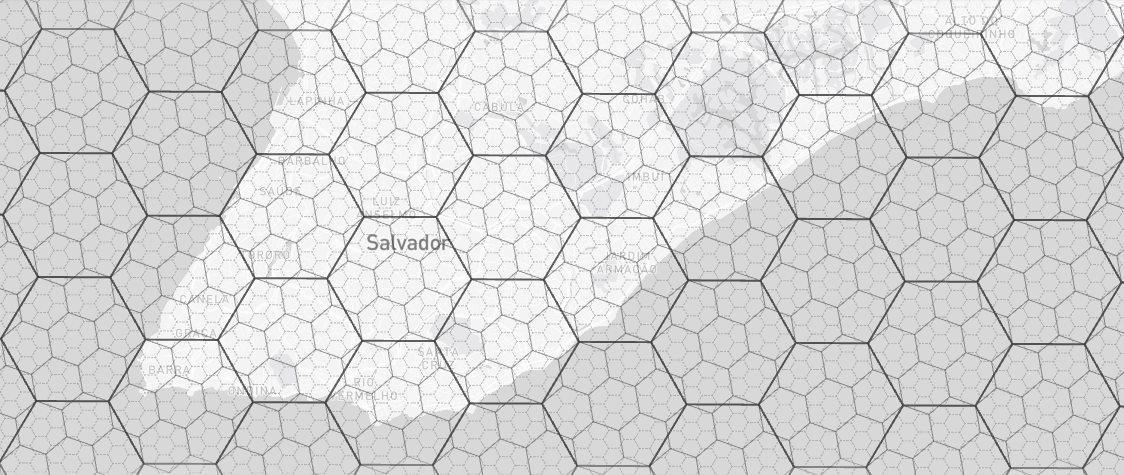
\includegraphics[keepaspectratio]{img/7-agregados/h3_ssa.png}}

}

\end{figure}%

Em relação às grades retangulares convencionais, grades hexagonais
apresentam algumas vantagens topológicas relevantes (Brodsky, 2018). Em
primeiro lugar, os hexágonos têm apenas um tipo de vizinho (os que
compartilham aresta), enquanto quadrados têm dois (aresta e vértice), o
que exige conjuntos distintos de coeficientes em análises. Em
decorrência desse aspecto, o centro de cada hexágono é equidistante dos
seis vizinhos, ao contrário das grades quadradas, onde os vizinhos
diagonais estão \textasciitilde41\% mais distantes que os laterais. Além
disso, anéis concêntricos de hexágonos aproximam círculos com mais
fidelidade do que anéis quadrados, tornando a análise de zonas de
influência e proximidade mais natural.

No Brasil, um caso de uso de destaque das grades hexagonais é o
\textbf{Projeto Acesso a Oportunidades} do IPEA (Pereira et al., 2022),
que disponibiliza dados censitários e de uso do solo em grade H3 de
resolução 9 para diversas cidades brasileiras, integrando informações
sobre distribuição espacial da população por idade, sexo, renda e raça,
além da localização de empregos e serviços públicos.

Contudo, transferir dados de setores censitários para outras unidades
espaciais não é uma tarefa trivial. A abordagem mais simples, que
distribui os dados proporcionalmente à área de sobreposição entre os
setores e as unidades-alvo, ignora que a população não está distribuída
uniformemente pelo espaço. Uma quadra residencial densa e um parque
urbano podem estar no mesmo setor e ter a mesma área, mas a população se
concentra na quadra.

\subsection{\texorpdfstring{Interpolação dasimétrica com o pacote
\texttt{cnefetools}}{Interpolação dasimétrica com o pacote cnefetools}}\label{interpolauxe7uxe3o-dasimuxe9trica-com-o-pacote-cnefetools}

Uma possível solução para esse problema é a \textbf{interpolação
dasimétrica} (\emph{dasymetric interpolation}), uma técnica que usa
informações espaciais auxiliares para guiar a redistribuição espacial
dos dados (Mennis, 2003). No contexto do Censo brasileiro, o Cadastro
Nacional de Endereços para Fins Estatísticos (CNEFE, um dos produtos do
Censo que abordaremos em um outro capítulo mais adiante) oferece um
insumo interessante para este propósito: a localização de cada endereço
visitado pelos recenseadores.

O pacote
\href{https://github.com/pedreirajr/cnefetools}{\texttt{cnefetools}}
(Pedreira Junior \& Stabile, 2026) implementa esse fluxo de trabalho de
forma integrada, combinando automaticamente os dados do CNEFE com os
agregados por setor para produzir estimativas em outras configurações
espaciais. As funções do pacote que executam esse processo são:

\begin{itemize}
\tightlist
\item
  \texttt{tracts\_to\_h3()}: transfere variáveis dos setores para uma
  grade de hexágonos H3 na resolução desejada.
\item
  \texttt{tracts\_to\_polygon()}: transfere variáveis dos setores para
  qualquer tipo de malha de polígonos fornecida pelo usuário.
\end{itemize}

Em vez de assumir distribuição uniforme por área, a interpolação
dasimétrica distribui os dados do setor pelos pontos de endereços que
estão dentro dele e, em seguida, agrega os valores dos pontos que caem
em cada unidade-alvo, conforme ilustrado na Figura~\ref{fig-dasyinter}.

\begin{figure}[H]

\caption{\label{fig-dasyinter}Esquema da interpolação dasimétrica usando
pontos de endereços do CNEFE como guia de distribuição espacial. Os
dados do setor censitário são alocados aos pontos de endereço e depois
agregados às unidades-alvo (hexágonos, zonas de tráfego etc.).}

\centering{

\pandocbounded{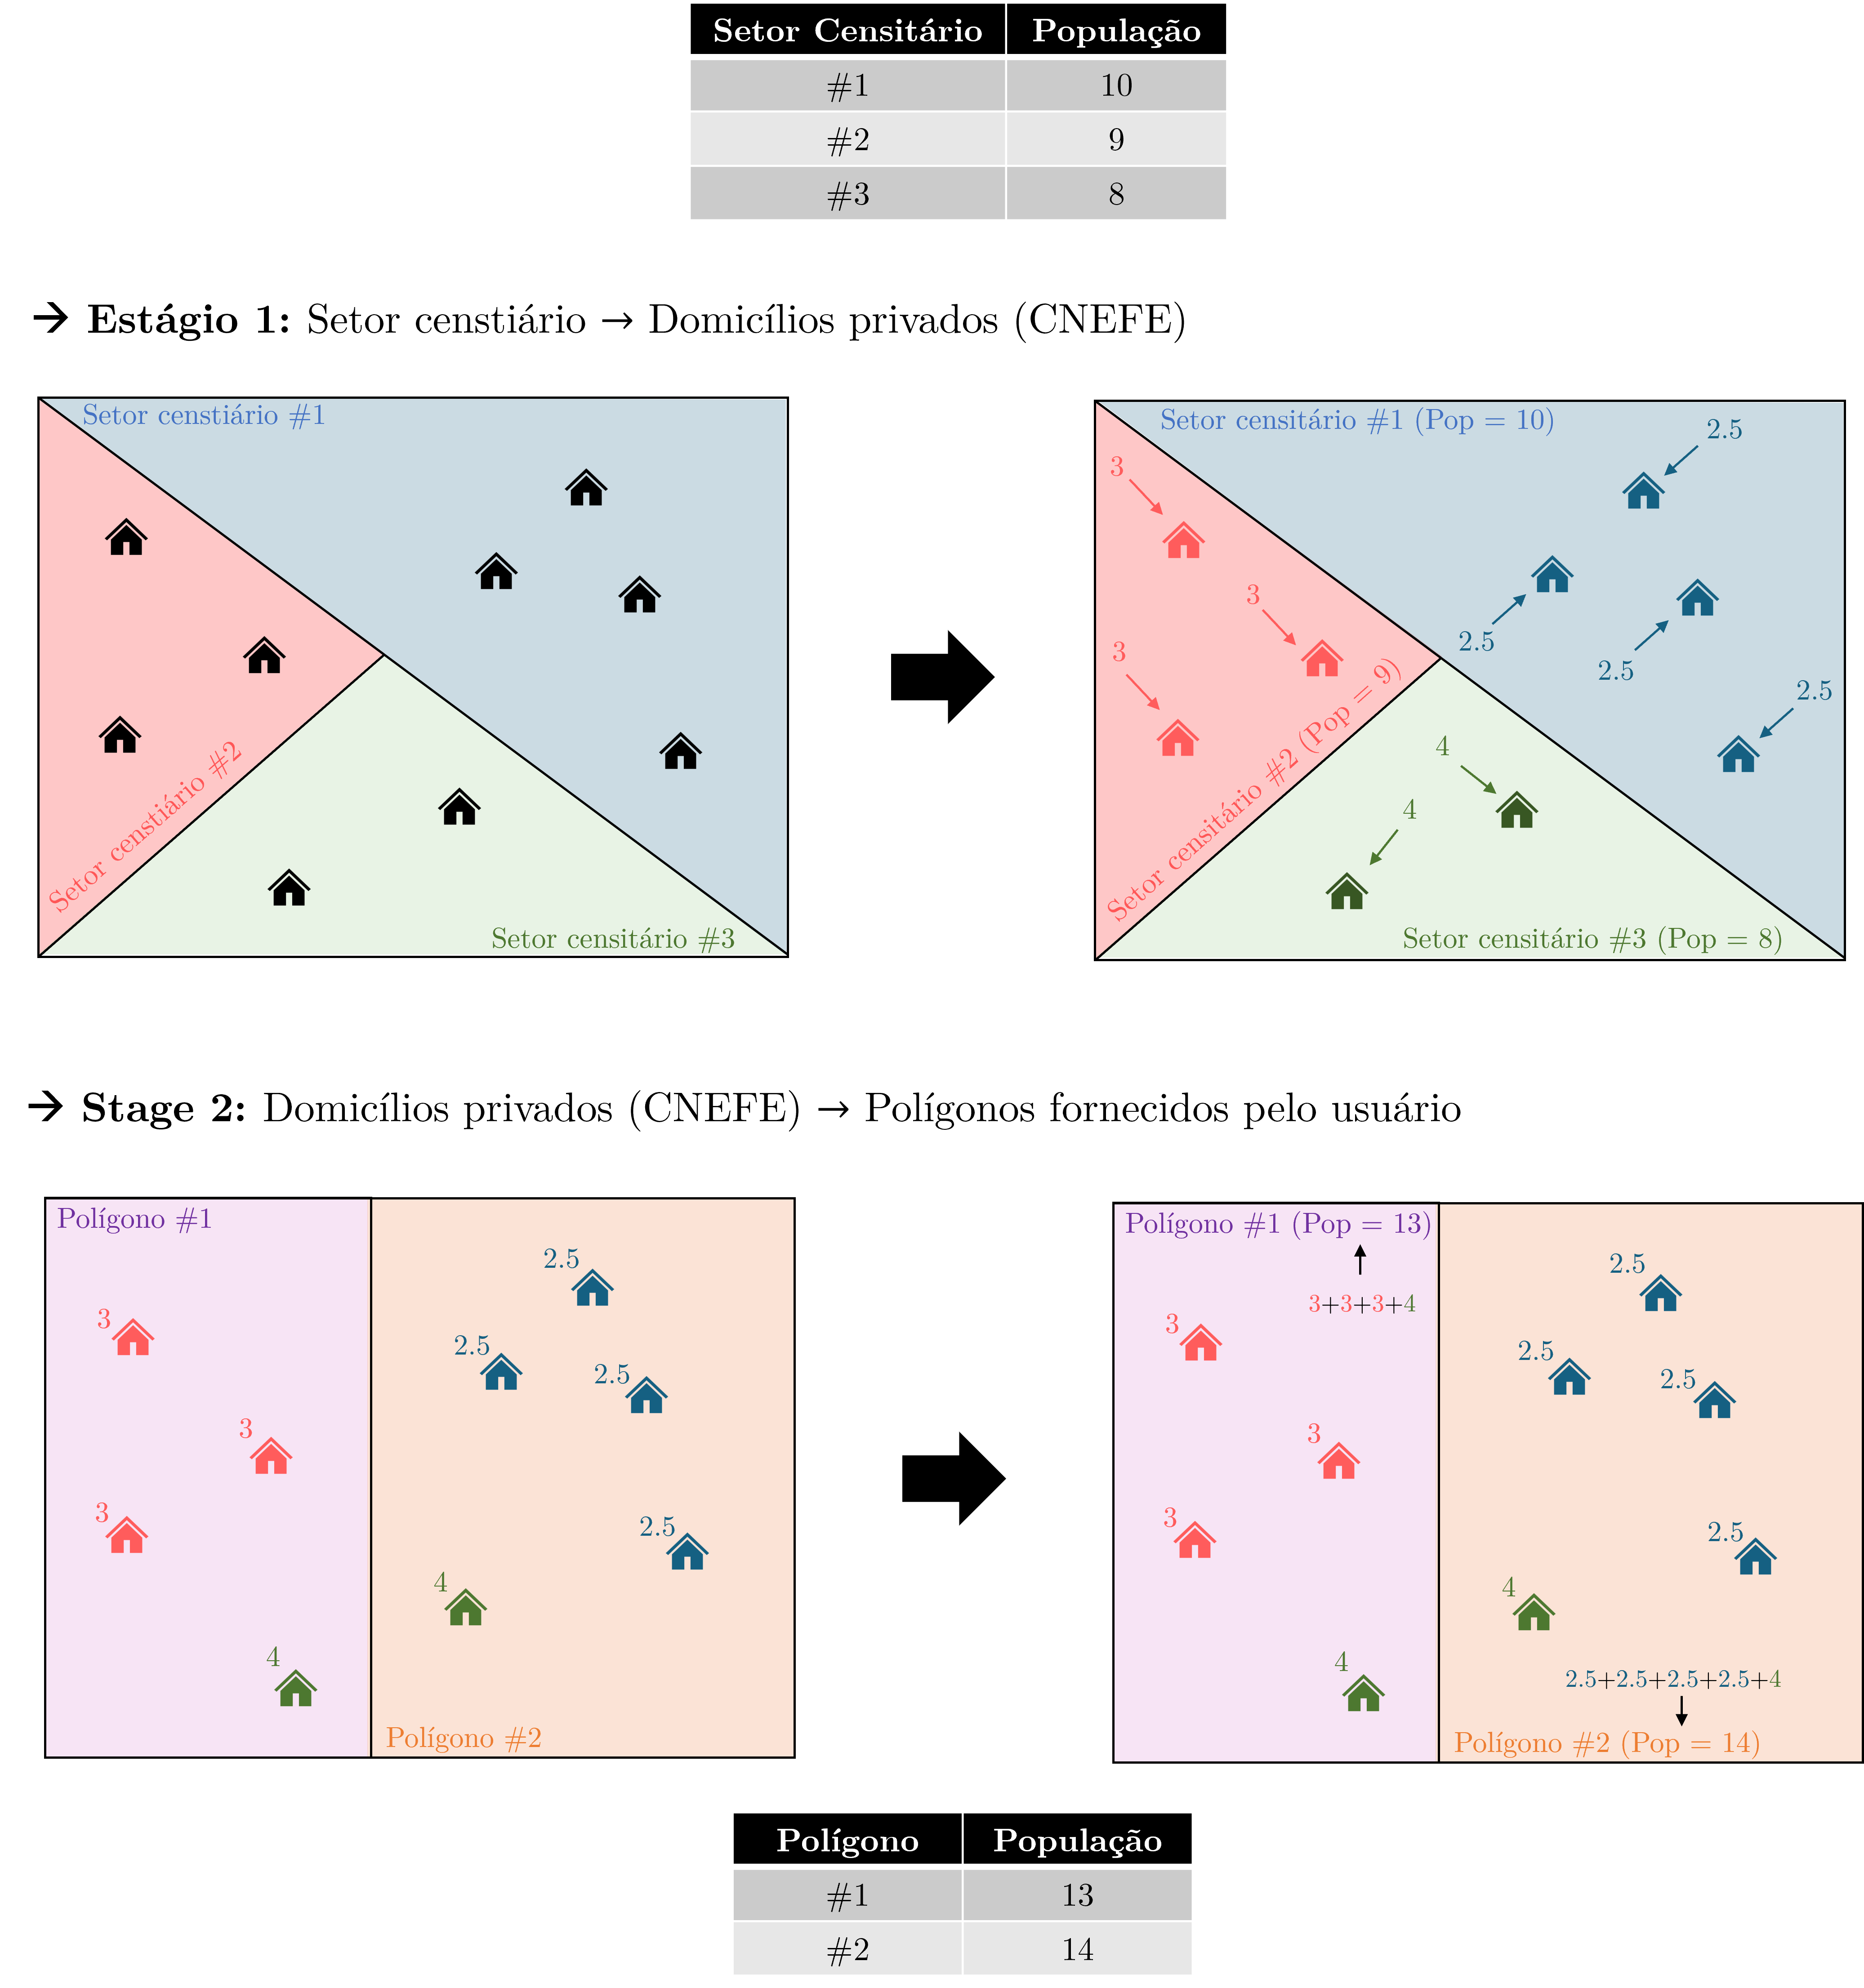
\includegraphics[keepaspectratio]{img/7-agregados/dasyinter.png}}

}

\end{figure}%

O argumento \texttt{vars} de ambas as funções aceita os nomes de
variáveis listados na Tabela~\ref{tbl-cnefetools-vars}. Para cada
variável, o pacote identifica automaticamente o tipo de alocação
adequado (total ou média) com base em uma tabela de referência interna
(\texttt{tracts\_variables\_ref}).

{

\begin{longtable}[]{@{}
  >{\centering\arraybackslash}p{(\linewidth - 6\tabcolsep) * \real{0.1650}}
  >{\centering\arraybackslash}p{(\linewidth - 6\tabcolsep) * \real{0.1262}}
  >{\centering\arraybackslash}p{(\linewidth - 6\tabcolsep) * \real{0.6408}}
  >{\centering\arraybackslash}p{(\linewidth - 6\tabcolsep) * \real{0.0680}}@{}}

\caption{\label{tbl-cnefetools-vars}Variáveis disponíveis para
interpolação dasimétrica no \texttt{cnefetools}. Fonte:
\texttt{cnefetools::tracts\_variables\_ref}.}

\tabularnewline

\toprule\noalign{}
\begin{minipage}[b]{\linewidth}\centering
Variável
\end{minipage} & \begin{minipage}[b]{\linewidth}\centering
Código IBGE
\end{minipage} & \begin{minipage}[b]{\linewidth}\centering
Descrição
\end{minipage} & \begin{minipage}[b]{\linewidth}\centering
Tipo
\end{minipage} \\
\midrule\noalign{}
\endhead
\bottomrule\noalign{}
\endlastfoot
\texttt{pop\_ph} & V00005 & Moradores em dom. particulares permanentes
ocupados & Total \\
\texttt{pop\_ch} & V00007 & Moradores em dom. coletivos com morador &
Total \\
\texttt{male} & V01007 & Pessoas do sexo masculino & Total \\
\texttt{female} & V01008 & Pessoas do sexo feminino & Total \\
\texttt{age\_0\_4} & V01031 & Pessoas de 0 a 4 anos & Total \\
\texttt{age\_5\_9} & V01032 & Pessoas de 5 a 9 anos & Total \\
\texttt{age\_10\_14} & V01033 & Pessoas de 10 a 14 anos & Total \\
\texttt{age\_15\_19} & V01034 & Pessoas de 15 a 19 anos & Total \\
\texttt{age\_20\_24} & V01035 & Pessoas de 20 a 24 anos & Total \\
\texttt{age\_25\_29} & V01036 & Pessoas de 25 a 29 anos & Total \\
\texttt{age\_30\_39} & V01037 & Pessoas de 30 a 39 anos & Total \\
\texttt{age\_40\_49} & V01038 & Pessoas de 40 a 49 anos & Total \\
\texttt{age\_50\_59} & V01039 & Pessoas de 50 a 59 anos & Total \\
\texttt{age\_60\_69} & V01040 & Pessoas de 60 a 69 anos & Total \\
\texttt{age\_70m} & V01041 & Pessoas de 70 anos ou mais & Total \\
\texttt{race\_branca} & V01317 & Pessoas de cor ou raça branca &
Total \\
\texttt{race\_preta} & V01318 & Pessoas de cor ou raça preta & Total \\
\texttt{race\_parda} & V01320 & Pessoas de cor ou raça parda & Total \\
\texttt{race\_amarela} & V01319 & Pessoas de cor ou raça amarela &
Total \\
\texttt{race\_indigena} & V01321 & Pessoas de cor ou raça indígena &
Total \\
\texttt{n\_resp} & V06001 & Responsáveis por dom. particulares
permanentes ocupados & Total \\
\texttt{avg\_inc\_resp} & V06004 & Rendimento nominal médio mensal dos
responsáveis com rendimentos & Média \\

\end{longtable}

}

É importante salientar que o método funciona de maneira diferente para
dois tipos de variáveis:

\begin{itemize}
\tightlist
\item
  \textbf{Variáveis de totais} (como população total ou quantidade de
  indivíduos do sexo feminino): o total do setor é dividido igualmente
  entre os pontos de endereço elegíveis dentro dele. Cada unidade
  espacial alvo recebe, então, a soma dos valores dos pontos que caem
  dentro de seus limites. Corresponde exatamente ao que é demonstrado na
  Figura~\ref{fig-dasyinter}.
\item
  \textbf{Variáveis de média} (a única: rendimento nominal médio mensal
  dos responsáveis com rendimento): o valor médio do setor é atribuído a
  cada ponto. A unidade espacial alvo recebe a média dos valores dos
  pontos que estão dentro dela.
\end{itemize}

\subsection{Interpolando para hexágonos
H3}\label{interpolando-para-hexuxe1gonos-h3}

Entendidos estes aspectos preliminares, podemos então produzir alguns
resultados. O código a seguir gera uma grade de hexágonos H3 (resolução
8, definido no argumento \texttt{h3\_resolution}) para Recife com a
variável de população total em domicílios particulares permanentes
(\texttt{pop\_ph}) a partir da função \texttt{tracts\_to\_h3()}:

\begin{Shaded}
\begin{Highlighting}[]
\FunctionTok{library}\NormalTok{(cnefetools)}

\NormalTok{hex\_recife }\OtherTok{\textless{}{-}} \FunctionTok{tracts\_to\_h3}\NormalTok{(}
  \AttributeTok{code\_muni     =} \DecValTok{2611606}\NormalTok{,}
  \AttributeTok{h3\_resolution =} \DecValTok{8}\NormalTok{,}
  \AttributeTok{vars          =} \StringTok{"pop\_ph"}
\NormalTok{)}
\end{Highlighting}
\end{Shaded}

A população de domicílios privados do arquivo geográfico
\texttt{hex\_recife} produzido pela \texttt{tracts\_to\_h3()}
anteriormente pode ser então visualizado de forma interativa com
\texttt{mapview}, conforme o código abaixo:

\begin{Shaded}
\begin{Highlighting}[]
\FunctionTok{mapview}\NormalTok{(hex\_recife,}
        \AttributeTok{zcol        =} \StringTok{"pop\_ph"}\NormalTok{,}
        \AttributeTok{layer.name  =} \StringTok{"Habitantes (estimativa)"}\NormalTok{,}
        \AttributeTok{col.regions =} \FunctionTok{hcl.colors}\NormalTok{(}\DecValTok{100}\NormalTok{, }\AttributeTok{palette =} \StringTok{"YlOrRd"}\NormalTok{) }\SpecialCharTok{|\textgreater{}} \FunctionTok{rev}\NormalTok{())}
\end{Highlighting}
\end{Shaded}

\pandocbounded{\includegraphics[keepaspectratio]{7-agregados_files/figure-pdf/unnamed-chunk-14-1.pdf}}

\subsection{Interpolando para malhas poligonais de qualquer
tipo}\label{interpolando-para-malhas-poligonais-de-qualquer-tipo}

Apesar de bastante úteis, nem sempre estamos interessados em produzir
informações do Censo em grades regulares (hexagonais ou não). No
contexto do planejamento de transportes, por exemplo, é muito comum
trabalharmos com a representação espacial de \textbf{zonas de tráfego}
para subdividir o território. Estas são as unidades espaciais básicas
usadas nos modelos de demanda por transporte, onde zona é delimitada de
modo que os deslocamentos entre origens e destinos diferentes possam ser
representados como fluxos entre pares de zonas.

Na prática, seus limites são definidos respeitando divisores naturais
como vias expressas, linhas férreas e rios. Neste desenho, é importante
também que o total de viagens internas (com origem e destino dentro de
cada zona) não sejam maiores que um determinado limite. O
\href{https://www.gov.br/dnit/pt-br/assuntos/planejamento-e-pesquisa/ipr/coletanea-de-manuais/vigentes/723_manual_estudos_trafego.pdf}{Manual
de Estudos de Tráfego} do Departamento Nacional de Infraestrutura de
Transportes (DNIT, 2006), por exemplo, preconiza que as zonas não tenham
tráfego local superior a 15\% do seu total de viagens. Tais
recomendações podem implicar que as fronteira dos setores censitários
não sejam úteis para estudos de transporte, o que torna necessária
alguma forma de interpolação para alocar variáveis socioeconômicas às
zonas.

Considerando este contexto, nosso objetivo será produzir dados
censitários para zonas de tráfego a partir da função
\texttt{tracts\_to\_polygon()}. Utilizaremos o município de São Paulo
como estudo de caso, a partir das suas zonas de tráfego produzidas na
Pesquisa Origem-Destino (OD) de 2017, realizada pelo Metrô de São Paulo.
Esse arquivo geográfico será obtido a partir do pacote
\href{https://github.com/hsvab/odbr}{\texttt{odbr}} (Svab et al., 2023),
que traz também os microdados desta pesquisa.

Como a pesquisa cobre toda a região metropolitana (39 municípios),
filtraremos apenas as zonas do município de São Paulo-SP através do
campo \texttt{NomeMunici}:

\begin{Shaded}
\begin{Highlighting}[]
\FunctionTok{library}\NormalTok{(cnefetools)}
\FunctionTok{library}\NormalTok{(odbr)}

\CommentTok{\# Zonas de tráfego da Pesquisa OD 2017 — Região Metropolitana de SP}
\NormalTok{sp\_zones }\OtherTok{\textless{}{-}} \FunctionTok{read\_map}\NormalTok{(}
  \AttributeTok{city     =} \StringTok{"Sao Paulo"}\NormalTok{,}
  \AttributeTok{year     =} \DecValTok{2017}\NormalTok{,}
  \AttributeTok{geometry =} \StringTok{"zone"}
\NormalTok{)}

\CommentTok{\# Filtrando apenas as zonas do município de São Paulo}
\NormalTok{sp\_zones\_muni }\OtherTok{\textless{}{-}}\NormalTok{ sp\_zones }\SpecialCharTok{|\textgreater{}}
  \FunctionTok{filter}\NormalTok{(NomeMunici }\SpecialCharTok{==} \StringTok{"São Paulo"}\NormalTok{) }\SpecialCharTok{|\textgreater{}}
\NormalTok{  sf}\SpecialCharTok{::}\FunctionTok{st\_make\_valid}\NormalTok{()}
\end{Highlighting}
\end{Shaded}

Utilizamos então essa malha poligonal \texttt{sp\_zones\_muni} como
valor do argumento \texttt{polygon} da função
\texttt{tracts\_to\_polygon()}, e escolhemos a população de domicílios
privados (\texttt{pop\_ph}) e a população com 70 anos ou mais
(\texttt{age\_70m}) para interpolar para as zonas de tráfego:

\begin{Shaded}
\begin{Highlighting}[]
\CommentTok{\# Transferindo população total e idosos dos setores para as zonas}
\NormalTok{sp\_zones\_census }\OtherTok{\textless{}{-}} \FunctionTok{tracts\_to\_polygon}\NormalTok{(}
  \AttributeTok{code\_muni =} \DecValTok{3550308}\NormalTok{,}
  \AttributeTok{polygon   =}\NormalTok{ sp\_zones\_muni,}
  \AttributeTok{vars      =} \FunctionTok{c}\NormalTok{(}\StringTok{"pop\_ph"}\NormalTok{, }\StringTok{"age\_70m"}\NormalTok{)}
\NormalTok{)}
\end{Highlighting}
\end{Shaded}

Por fim, produzimos um mapa da variável relativa à população de 70 anos
ou mais nas zonas de tráfego, originalmente advinda dos agregados:

\begin{Shaded}
\begin{Highlighting}[]
\CommentTok{\# Proporção de população com 70 anos ou mais por zona}
\NormalTok{sp\_zones\_ratio }\OtherTok{\textless{}{-}}\NormalTok{ sp\_zones\_census }\SpecialCharTok{|\textgreater{}}
  \FunctionTok{filter}\NormalTok{(pop\_ph }\SpecialCharTok{\textgreater{}} \DecValTok{0}\NormalTok{) }\SpecialCharTok{|\textgreater{}}
  \FunctionTok{mutate}\NormalTok{(}\AttributeTok{pct\_70m =}\NormalTok{ age\_70m }\SpecialCharTok{/}\NormalTok{ pop\_ph)}

\FunctionTok{mapview}\NormalTok{(sp\_zones\_ratio, }\AttributeTok{zcol =} \StringTok{"pct\_70m"}\NormalTok{, }\AttributeTok{layer.name =} \StringTok{"Prop. pop. 70+"}\NormalTok{)}
\end{Highlighting}
\end{Shaded}

\begin{Shaded}
\begin{Highlighting}[]
\FunctionTok{mapview}\NormalTok{(sp\_zones\_ratio,}
        \AttributeTok{zcol       =} \StringTok{"pct\_70m"}\NormalTok{,}
        \AttributeTok{layer.name =} \StringTok{"Prop. pop. 70+"}\NormalTok{)}
\end{Highlighting}
\end{Shaded}

\pandocbounded{\includegraphics[keepaspectratio]{7-agregados_files/figure-pdf/unnamed-chunk-19-1.pdf}}

\subsection{\texorpdfstring{Ressalvas com o uso da interpolação do
\texttt{cnefetools}}{Ressalvas com o uso da interpolação do cnefetools}}\label{ressalvas-com-o-uso-da-interpolauxe7uxe3o-do-cnefetools}

A interpolação dasimétrica implementada no \texttt{cnefetools}
representa um avanço em relação à interpolação por área convencional,
mas não elimina todos os problemas de inferência espacial. É importante
ter em mente duas limitações relevantes antes de interpretar os
resultados.

A primeira diz respeito à \textbf{falácia ecológica}. O método assume
que todos os domicílios de um setor censitário são razoavelmente
uniformes em relação à variável interpolada, pois cada ponto de endereço
dentro do setor recebe a mesma fração do total ou o mesmo valor médio.
Na prática, um setor pode conter domicílios de perfis socioeconômicos
distintos, e a alocação uniforme ignora essa heterogeneidade interna. O
resultado é que a variável estimada para a unidade-alvo reflete a média
do setor de origem, não necessariamente a composição real dos endereços
que caem dentro daquela unidade. Quanto menor e mais homogêneo for o
setor censitário em relação à variável de interesse, menor será esse
viés.

A segunda limitação refere-se às \textbf{unidades nas bordas
municipais}. Quando uma zona de tráfego (ou hexágono) cruza o limite do
município, ela recebe apenas os endereços do município informado em
\texttt{code\_muni}. Os endereços do município vizinho não são
incluídos, pois o \texttt{cnefetools} opera sobre o CNEFE de um
município de cada vez. Isso significa que as estatísticas calculadas
para unidades na borda representam apenas a parcela que pertence ao
\texttt{code\_muni} informado. Em análises de regiões metropolitanas,
onde os limites municipais cruzam frequentemente áreas contínuas de
ocupação, essa limitação deve ser levada em consideração na
interpretação dos resultados.

\section{Exercícios}\label{exercuxedcios-5}

\begin{enumerate}
\def\labelenumi{\arabic{enumi}.}
\item
  Utilizando o fluxo apresentado na Seção~\ref{sec-obtendo}, calcule
  para o município de \textbf{Fortaleza (CE)} a proporção de domicílios
  com coleta de lixo direta (consulte o dicionário para identificar a
  variável correspondente no arquivo Domicílio). Visualize o resultado
  em um mapa com \texttt{mapview}.
\item
  Selecione duas variáveis de diferentes arquivos temáticos (por
  exemplo, uma de demografia e uma de domicílios) e construa um mapa
  coropléfico com \texttt{ggplot2} para um município de sua escolha.
  Inclua título, legenda e fonte nos atributos do mapa.
\item
  Para o município de Salvador, reproduza os dois mapas de proporção
  produzidos neste capítulo, o de domicílios sem abastecimento pela rede
  geral e o de domicílios sem esgotamento por rede geral ou fossa
  séptica ligada. Em quais regiões do município as duas carências
  ocorrem simultaneamente? Como você interpretaria esse padrão em termos
  de planejamento urbano?
\item
  Pesquise a documentação do pacote \texttt{cnefetools} e identifique
  quais variáveis estão disponíveis para interpolação dasimétrica com
  \texttt{tracts\_to\_h3()}. Aplique a função para gerar uma grade H3
  (resolução 7) para \textbf{Salvador (BA)} com pelo menos duas
  variáveis e discuta esses resultados.
\end{enumerate}

\chapter{Microdados da Amostra}\label{microdados-da-amostra}

\section{Introdução}\label{introduuxe7uxe3o-2}

Nos dois capítulos anteriores, introduzimos conceitualmente o Censo
Demográfico e aprendemos a explorar um dos seus principais produtos, os
Agregados por Setor Censitário. Todavia, os Agregados são limitados com
relação aos aspectos sociodemográficos que são possíveis de analisar a
partir do Censo, já que se referem somente aos itens levantados no
Questionário Básico. Neste capítulo, apresentaremos um produto distinto
e complementar, os \textbf{microdados da amostra do Censo Demográfico},
que permitem análises muito mais ricas em termos de variáveis, embora ao
custo de uma resolução espacial menor.

A modalidade amostral do Censo
\href{https://www.ibge.gov.br/estatisticas/sociais/saude/9662-censo-demografico-2010.html?edicao=9754&t=conceitos-e-metodos}{tem
raízes na edição de 1960}, quando o Brasil adotou técnicas de amostragem
probabilística na coleta censitária. A partir de então, passou-se a
utilizar dois tipos de questionário para as entrevistas domiciliares, o
Básico e o da Amostra, que seguem até os dias atuais. Os microdados são
a forma mais desagregada de divulgação dos Resultados da Amostra, com os
registros individuais\footnote{daí se origina a nomenclatura
  \emph{microdados}} de cada domicílio e morador entrevistados.

Ao contrário dos agregados por setor, os microdados não vêm com totais
pré-calculados para áreas diferentes do território, mas sim com os
valores individuais de cada variável para cada domicílio ou pessoa. É o
pesquisador quem decide quais estatísticas calcular e como organizá-las.
Essa riqueza temática é possível porque os microdados registram todas as
variáveis do \textbf{Questionário da Amostra}, o instrumento mais
completo do Censo. Esse questionário contém todos os quesitos do
Questionário Básico (26 questões no Censo 2022 e 34 no de 2010) e um
conjunto adicional de temas, como outras características dos domicílios
(ex.: acesso a Internet e quantidade de cômodos) e dos indivíduos (ex.:
nupcialidade, fecundidade, religião, deficiência, migração e
deslocamento para estudo/trabalho) (IBGE, 2024c). Em 2022, o
questionário da amostra foi composto 77 questões, uma redução importante
em relação ao questionário de 2010, que contava com 102 quesitos. Em
ambas as edições, o questionário foi respondido por aproximadamente 1 de
cada 10 domicílios brasileiros.

Em contrapartida, a menor unidade geográfica identificável de cada
domicílio ou indivíduo nos microdados é a \textbf{área de ponderação},
um agrupamento de setores censitários descrito em detalhe na
Seção~\ref{sec-areas-pond}. Esse recorte é bastante mais amplo que o
setor censitário, já que uma área de ponderação contém, no mínimo, 400
domicílios particulares ocupados na amostra. Para se ter uma ideia, no
Censo de 2010, o maior município do país, São Paulo-SP, possuía 5.082
setores censitários e somente 107 áreas de ponderação. Em municípios
menores, ela corresponde ao município inteiro. Isso significa que
análises espacialmente detalhadas (como as possíveis com os Agregados e
a Grade Estatística) ficam fora do alcance dos microdados. No entanto,
para estudar variáveis que o Questionário Básico não cobre, os
microdados são o único caminho.

\begin{tcolorbox}[enhanced jigsaw, arc=.35mm, bottomrule=.15mm, bottomtitle=1mm, breakable, colback=white, colbacktitle=quarto-callout-warning-color!10!white, colframe=quarto-callout-warning-color-frame, coltitle=black, left=2mm, leftrule=.75mm, opacityback=0, opacitybacktitle=0.6, rightrule=.15mm, title=\textcolor{quarto-callout-warning-color}{\faExclamationTriangle}\hspace{0.5em}{Microdados do Censo 2022 ainda não disponíveis}, titlerule=0mm, toprule=.15mm, toptitle=1mm]

No momento da escrita deste capítulo (início de abril de 2026), o IBGE
ainda não havia divulgado os microdados da amostra do Censo Demográfico
2022. Todos os exemplos práticos das seções 4 e 5 utilizam dados do
Censo de 2010, acessados via pacote \texttt{censobr}. Os conceitos e
procedimentos apresentados são equivalentes para ambas as edições, e os
códigos deverão funcionar para 2022 com ajustes mínimos após a
divulgação dos dados.

\end{tcolorbox}

\section{Aspectos metodológicos}\label{aspectos-metodoluxf3gicos}

\subsection{O plano amostral}\label{o-plano-amostral}

Para o planejamento da coleta dos dados do Questionário da Amostra, o
IBGE realiza uma \textbf{amostragem probabilística} no interior de cada
setor censitário. Em cada setor, uma fração fixa de domicílios
particulares é selecionada por sorteio aleatório. Portanto, o setor
censitário é o \textbf{estrato} do plano, com a seleção ocorrendo de
forma independente dentro de cada um, onde nenhum domicílio é
selecionado com base no que ocorreu nos demais setores.

Quando um domicílio é selecionado, todos os seus moradores são
entrevistados. Isso cria dois regimes de amostragem distintos para os
dois arquivos de microdados, cuja distinção tem consequências diretas
para a análise, como veremos na Seção~\ref{sec-survey}:

\begin{itemize}
\tightlist
\item
  \textbf{Microdados de domicílios:} amostragem aleatória estratificada
  de domicílios, com estratos nos setores censitários.
\item
  \textbf{Microdados de pessoas:} amostragem estratificada e
  conglomerada, com estratificação nos setores censitários (estratos =
  setores censitários) e conglomeração nos domicílios (conglomerados =
  domicílios). Isso significa que os indivíduos não são sorteados
  diretamente, mas compõem um conglomerado inserido em um domicílio que
  foi selecionado.
\end{itemize}

A fração amostral aplicada aos setores depende do porte do município ao
qual pertencem. Para os dois últimos Censos (2010 e 2022), estes valores
foram os mesmos, conforme se observa na Tabela~\ref{tbl-fracoes}. Isso
resultou em 6,2 milhões de domicílios com 20,6 milhões de pessoas no
Censo de 2010 e 7,8 milhões de domicílios com 21,9 milhões de pessoas no
Censo de 2022 (IBGE, 2016b, 2024c). Em ambos os casos, temos quase 11\%
do total da população em análise respondendo ao Questionário da Amostra,
cujos dados exploraremos mais adiante.

\begin{longtable}[t]{cccc}

\caption{\label{tbl-fracoes}Frações amostrais dos Censo Demográficos de
2010 e 2022 por porte do município. Fonte: IBGE (2016b) e IBGE (2024c).}

\tabularnewline

\toprule
Porte do município (habitantes) & Nº Municípios (2010) & Nº Municípios (2022) & Fração (2010 e 2022)\\
\midrule
Até 2.500 & 260 & 289 & 50\%\\
2.501 a 8.000 & 1912 & 1808 & 33\%\\
8.001 a 20.000 & 1749 & 1673 & 20\%\\
20.001 a 500.000 & 1604 & 1751 & 10\%\\
Mais de 500.000 & 40 & 49 & 5\%\\
\bottomrule

\end{longtable}

A fração mais alta nos municípios menores garante que mesmo localidades
com poucos domicílios tenham amostras de tamanho suficiente para a
divulgação de resultados com qualidade estatística aceitável. Em
contrapartida, nos 49 municípios com mais de 500 mil habitantes em 2022,
a fração de 5\% já representa volumes consideráveis de domicílios
entrevistados.

Em ambas as edições, alguns distritos e subdistritos de grandes
municípios receberam frações maiores que a padrão municipal, para
viabilizar a divulgação de resultados em nível inframunicipal. Em 2022,
o procedimento foi estendido também a Terras Indígenas, Territórios
Quilombolas e Favelas e Comunidades Urbanas, que receberam frações
diferenciadas chegando a 100\% em alguns casos (IBGE, 2024c).

\subsection{Expansão da amostra}\label{expansuxe3o-da-amostra}

Numa pesquisa por amostragem probabilística, cada domicílio selecionado
não representa apenas a si mesmo. Ele ``fala'' por outros domicílios que
não foram sorteados. Para quantificar essa representatividade, cada
domicílio da amostra recebe um \textbf{peso amostral}, que indica
quantos domicílios ele representa na população. Para esclarecer esse
processo, suponha um município hipotético com a configuração da
Figura~\ref{fig-config_cidade_hipo}, com os 105 domicílios distribuídos
em 3 áreas de ponderação e 5 setores censtiários.

\begin{figure}[H]

\caption{\label{fig-config_cidade_hipo}Município hipotético com 105
domicílios em 2 áreas de ponderação e 5 setores censitários}

\centering{

\pandocbounded{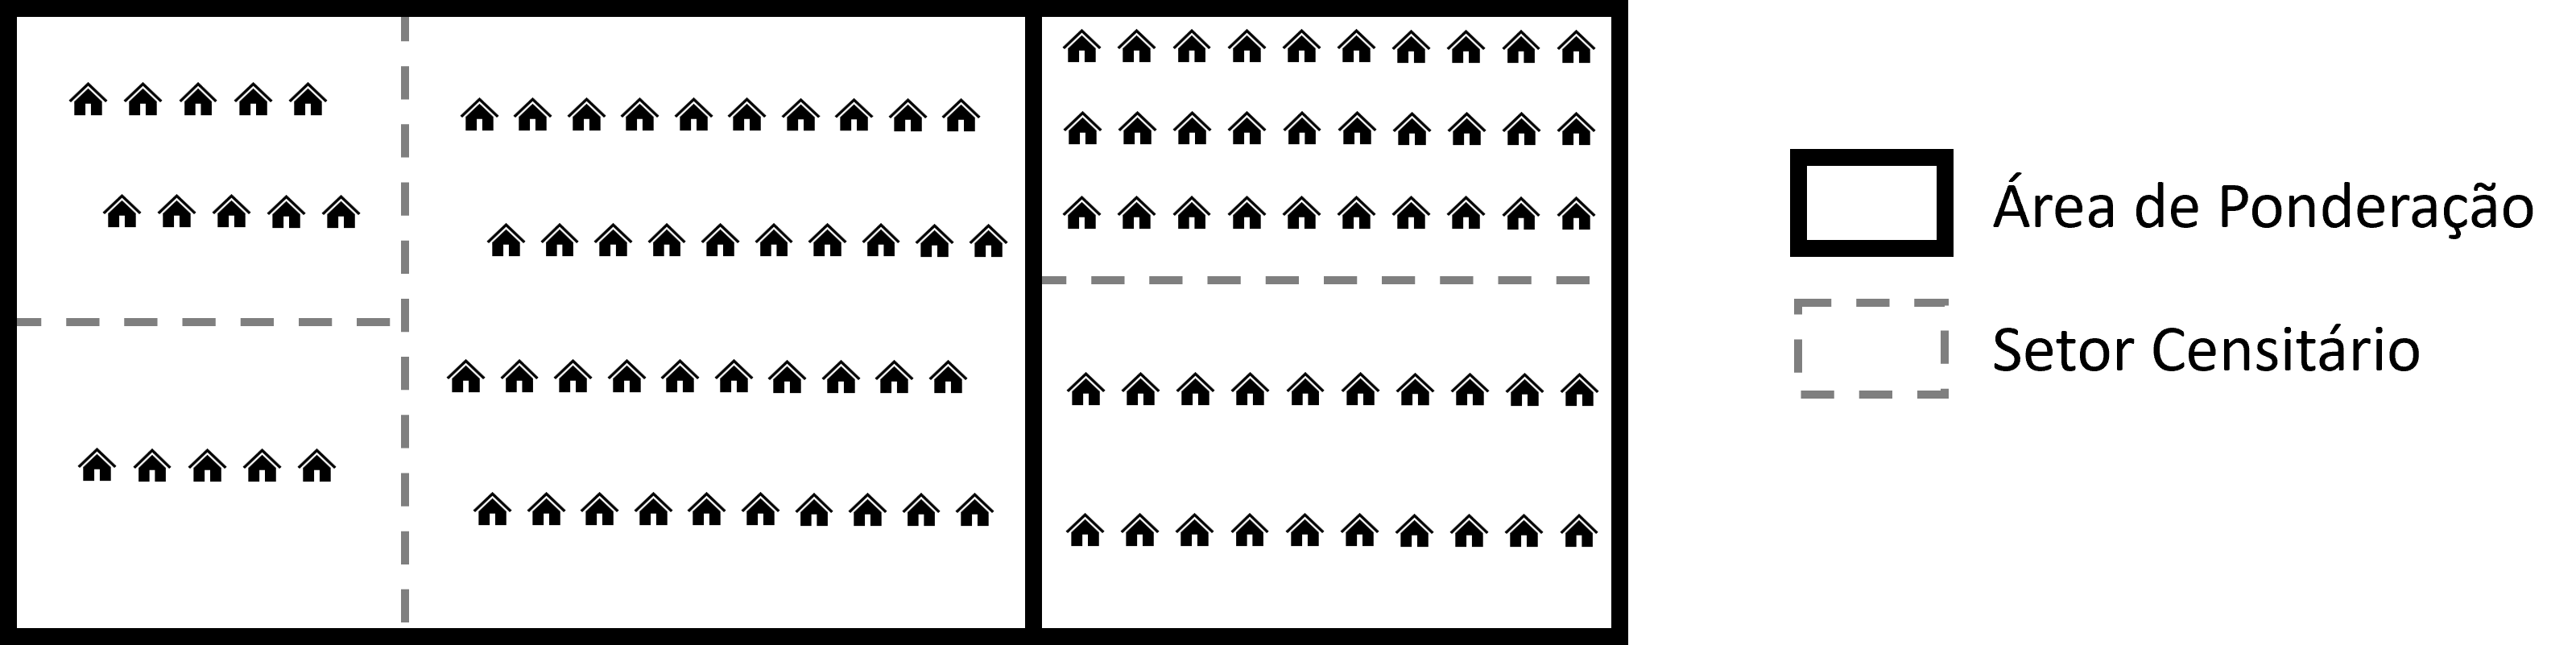
\includegraphics[keepaspectratio]{img/8-microdados/fig-config_cidade_hipo.png}}

}

\end{figure}%

Suponha que a fração amostral seja de 20\% para todo esse município,
implicando que 1 a cada 5 domicílios de cada setor censitário seja
selecionado para compor a amostra. Uma primeira aproximação para esse
peso é o inverso da fração amostral efetiva. Ou seja, cada domicílio
selecionado representa aproximadamente 5 outros domicílios (pois,
\(1/0,20 = 5\)). Deste modo, suponha que tenhamos selecionado
aleatoriamente os domicílios na cor vermelha conforme a
Figura~\ref{fig-domicilios_sorteados} no município hipotético. Nesse
processo, cada recebe peso amostral igual a 5 (ou seja, representam 5
domicílios em seu setor).

\begin{figure}[H]

\caption{\label{fig-domicilios_sorteados}Domicílios selecionados
aleatoriamente em cada setor censitário, de acordo com uma fração
amostral de 20\%}

\centering{

\pandocbounded{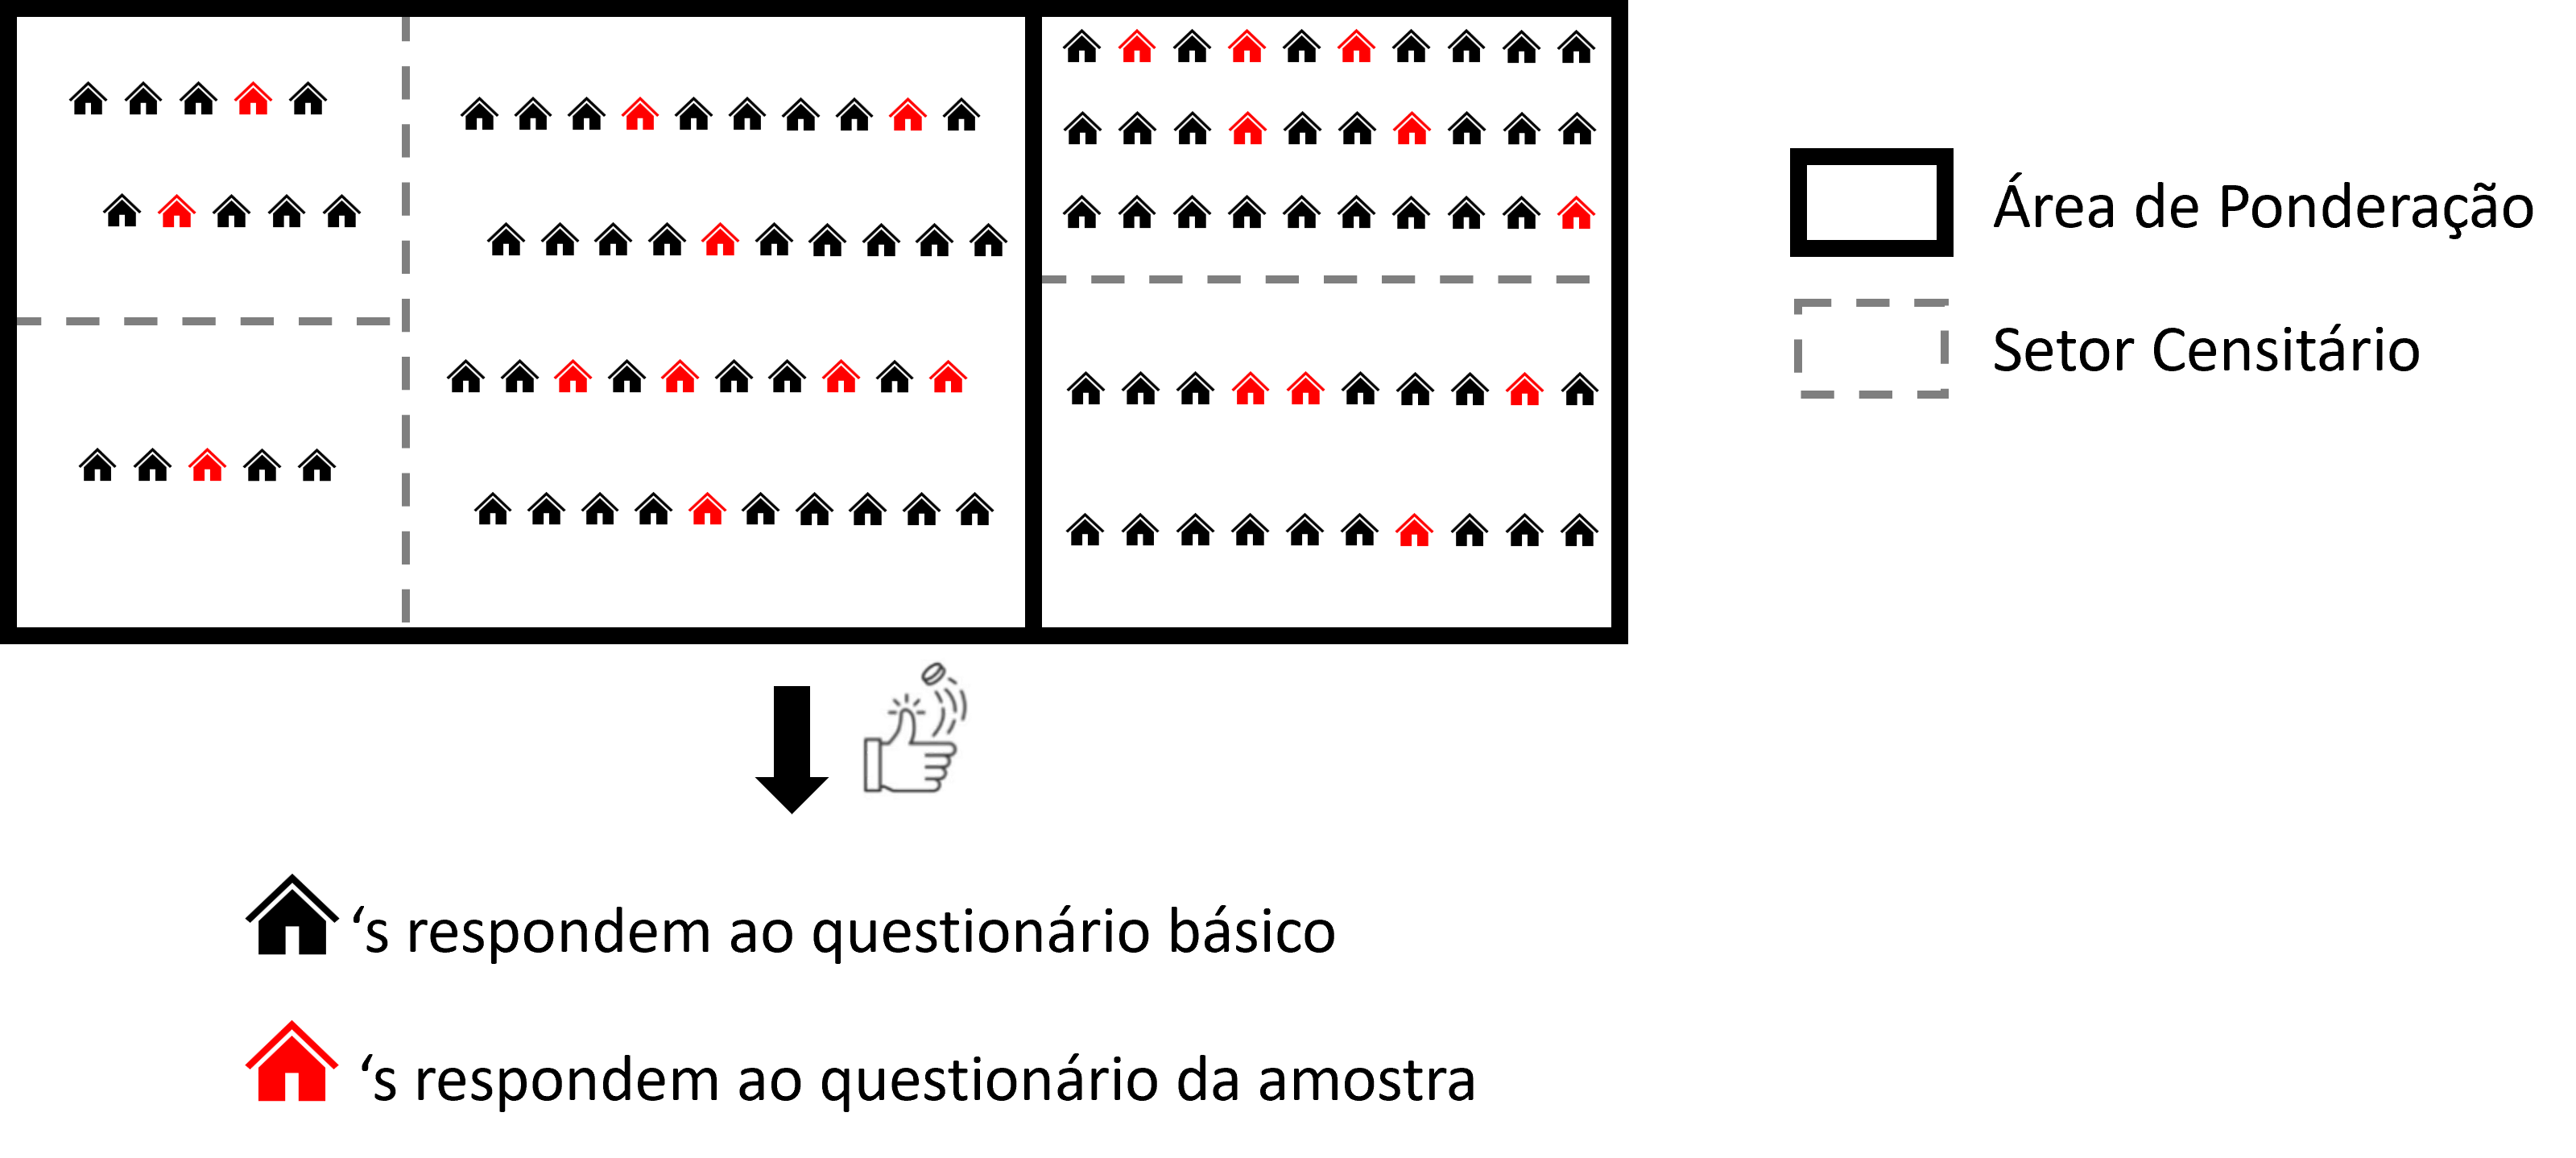
\includegraphics[keepaspectratio]{img/8-microdados/fig-domicilios_sorteados.png}}

}

\end{figure}%

Esse peso inicial, porém, pode não refletir adequadamente a distribuição
real da população. Por acaso, a amostra pode ter capturado um número
menor de pessoas de 0 a 15 anos ou mais pessoas do sexo feminino em
comparação ao que se sabe do universo naquela região. Para corrigir essa
variação aleatória, o IBGE realiza um processo de \textbf{calibração}
destes pesos.

A calibração consiste em ajustar os pesos iniciais de maneira que as
estimativas da amostra se aproximem dos totais já conhecidos para um
conjunto de variáveis \emph{auxiliares}. Tais variáveis são obtidas de
quesitos que existem em ambos os questionários (Básico e da Amostra), ou
seja, através delas conseguimos obter totais \textbf{populacionais
conhecidos} do processo de levantamento do Censo.

O método de calibração baseia-se em uma estratégia de Mínimos Quadrados
Generalizados (MQG), considerando as propostas de Bankier et al. (1992)
e Deville et al. (1993), similar ao empregado em censos de outros
países, como o canadense (IBGE, 2016b, 2024c; Statistics Canada, 2009).
Questões metodológicas específicas sobre amostragem complexa não são o
foco deste livro, mas o(a) leitor(a) interessado pode ganhar mais
profundidade teórica e prática consultando as obras de Silva et al.
(2021), Lumley (2011) e Zimmer et al. (2024).

É importante destacar que esse processo de calibração é realizado no
nível da área de \emph{ponderação}, que recebe esse nome justamente por
servir como unidade espacial onde se realiza a calibração dos pesos.
Nesse sentido, as \textbf{restrições de calibração} consistem em impor
que os totais populacionais das variáveis auxiliares se aproximem da
estimativa obtida a partir somente das informações da amostra expandida
(multiplicada por estes pesos) neste nível de desagregação espacial.

Em 2010, foram consideradas 40 restrições, incluindo total de pessoas,
total de domicílios, distribuição por sexo e faixas etárias detalhadas
(IBGE, 2016b). Em 2022, o conjunto foi ampliado para 47 restrições, com
a adição de Terras Indígenas, Territórios Quilombolas, Favelas e
Comunidades Urbanas, além de categorias de número de banheiros nos
domicílios particulares permanentes (IBGE, 2024c).

Nesse processo, há ainda a preocupação em evitar pesos extremos (muito
pequenos ou muito grandes) que poderiam distorcer as estimativas. Isso
se dá através da imposição de limites aos pesos calibrados. Na prática,
considerando os pesos inicial e calibrado de um domicílio \(i\) em uma
área de ponderação \(a\) como \(w_{ai}\) e \(w^*_{ai}\),
respectivamente, tem-se que os pesos calibrados não podem ser nem
inferiores a 1/5 (\(w^*_{ai} \ge w_{ai}/5\)) nem superiores a 5 vezes
(\(w^*_{ai}\le 5w_{ai}\)) o valor deste peso inicial (IBGE, 2024c).

O produto final é um único peso calibrado para cada domicílio da
amostra, que é replicado para todos os seus moradores. Esse peso,
armazenado na variável \texttt{V0010} para a base de microdados do Censo
de 2010, é o que utilizaremos em toda a análise. O IBGE recomenda que
ele seja mantido como valor fracionário (com 10 casas decimais), pois o
arredondamento para valores inteiros rompe a consistência das restrições
de calibração (IBGE, 2024c).

Na tabela da Figura~\ref{fig-vars_aux_censo22} abaixo, obtida de um
\emph{screenshot} do documento metodológico do Censo de 2022 (IBGE,
2024c), é possível evidenciar o resultado desse processo, comparando as
diferenças entre os totais observados e os totais estimados com os pesos
amostrais calibrados. Observe, as diferenças são sempre menores que 1\%,
à exceção da variável \emph{Total de domicílios particulares permanentes
sem banheiro} (\textasciitilde1,35\%).

\begin{figure}[H]

\caption{\label{fig-vars_aux_censo22}Comparação entre os totais
observados e com peso de cada variável auxiliar da calibração para o
Censo de 2022. Fonte: IBGE (2024c)}

\centering{

\pandocbounded{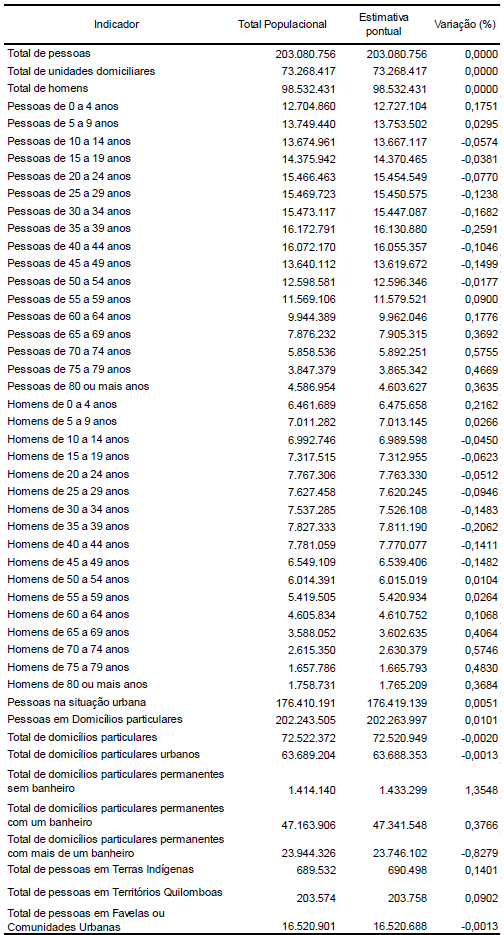
\includegraphics[keepaspectratio]{img/8-microdados/fig-vars_aux_censo22.png}}

}

\end{figure}%

\subsection{Áreas de ponderação (aspectos
metodológicos)}\label{sec-areas-pond}

Conforme mencionado anteriormente, a \textbf{área de ponderação} é o
recorte geográfico mais desagregado para o qual os microdados da amostra
podem ser divulgados publicamente. No Censo de 2010, estamos falando de
10.184 áreas de ponderação compreendendo os cerca de 313 mil setores
censitários. Para o Censo de 2022, temos, até o presente
momento\footnote{início de Abril de 2026}, somente áreas de ponderação
preliminares (cuja malha espacial não foi divulgada), com pesos
calibrados para a produção de alguns resultados parciais. Eles compõem
um total de 10.607 áreas de ponderação, que abrangem os 468 mil setores
censitários do país.

Dois critérios justificam essa escolha. O primeiro é a \textbf{precisão
estatística}, já que domínios geográficos muito pequenos produzem
estimativas com erros amostrais elevados. O segundo é a \textbf{proteção
da confidencialidade}, já que identificar unidades geográficas menores
nos microdados públicos permitiria, em muitas situações, identificar
domicílios ou indivíduos específicos.

A formação das áreas de ponderação obedece a três critérios simultâneos:
(i) \textbf{contiguidade} dos setores que a compõem; (ii)
\textbf{tamanho mínimo} de 400 domicílios particulares ocupados na
amostra; e (iii) \textbf{homogeneidade socioeconômica} interna. Em 2022,
a homogeneidade foi maximizada por um algoritmo baseado em oito
variáveis dos setores censitários, entre elas renda média do
responsável, proporção de domicílios na rede de esgoto e estrutura
etária da população (IBGE, 2024c).

O método de formação varia conforme o porte do município. Em municípios
com menos de 100 mil habitantes nos quais é possível formar pelo menos
duas áreas, o processo é automático, via algoritmo em R desenvolvido
pelo IBGE. Em municípios com mais de 100 mil habitantes, os técnicos do
Instituto realizam o agrupamento manualmente, utilizando as áreas de
ponderação do Censo 2010 como referência e fazendo ajustes com base em
critérios de homogeneidade e morfologia urbana. Municípios com uma única
área cobrem o território municipal por inteiro.

\section{Os pacotes survey e srvyr}\label{sec-survey}

Como discutido na seção anterior, os microdados da amostra têm uma
estrutura amostral complexa. A seleção foi feita por amostragem
estratificada (estratos nos setores censitários) nos domicílios, com uma
etapa adicional de conglomeração no caso de indivíduos. Cada observação
tem um peso diferente resultante da calibração. Calcular estatísticas
sem levar essa estrutura em conta produz estimativas que, para as médias
e totais, podem estar razoavelmente corretas, mas com
\textbf{erros-padrão incorretos} (geralmente subestimados). Isso faz com
que intervalos de confiança sejam mais estreitos do que deveriam, o que
pode levar a conclusões equivocadas sobre a significância das diferenças
encontradas.

O pacote \texttt{survey} para R (Lumley, 2023) foi desenvolvido
especificamente para lidar com esse problema. A ideia é implementar
estimadores e métodos de estimação de variância corretos para amostras
complexas, incorporando automaticamente os pesos, a estratificação e a
conglomeração em todos os cálculos. Vale salientar que o pacote
\texttt{survey} é inclusive a solução utilizada pelo corpo técnico do
IBGE no processo de calibração dos pesos desde o Censo de 2010 (IBGE,
2016b, 2024c). O ponto de partida é a criação de um \textbf{objeto de
desenho amostral} (\emph{survey design object}) com a função
\texttt{svydesign()}, que armazena os dados junto com a especificação do
plano de amostragem. Todas as funções de análise recebem esse objeto em
vez do \emph{data frame} original.

Já o pacote \texttt{srvyr} (Ellis \& Schneider, 2023) é uma extensão do
\texttt{survey} que oferece uma interface no estilo tidyverse. O objeto
de desenho é criado com \texttt{as\_survey\_design()}, que aceita os
mesmos argumentos de \texttt{svydesign()} mas sem fórmulas, de modo a se
integrar naturalmente ao fluxo \texttt{\textbar{}\textgreater{}}. A
análise por grupos usa \texttt{group\_by()} e \texttt{summarize()},
exatamente como no \texttt{dplyr}.

A Tabela~\ref{tbl-survey-srvyr} apresenta as principais funções
equivalentes entre os dois pacotes.

{

\begin{longtable}[]{@{}
  >{\raggedright\arraybackslash}p{(\linewidth - 4\tabcolsep) * \real{0.3483}}
  >{\centering\arraybackslash}p{(\linewidth - 4\tabcolsep) * \real{0.1910}}
  >{\centering\arraybackslash}p{(\linewidth - 4\tabcolsep) * \real{0.4607}}@{}}

\caption{\label{tbl-survey-srvyr}Funções equivalentes nos pacotes
\texttt{survey} e \texttt{srvyr}.}

\tabularnewline

\toprule\noalign{}
\begin{minipage}[b]{\linewidth}\raggedright
Tarefa
\end{minipage} & \begin{minipage}[b]{\linewidth}\centering
\texttt{survey}
\end{minipage} & \begin{minipage}[b]{\linewidth}\centering
\texttt{srvyr}
\end{minipage} \\
\midrule\noalign{}
\endhead
\bottomrule\noalign{}
\endlastfoot
Criar objeto de plano amostral & \texttt{svydesign()} &
\texttt{as\_survey\_design()} \\
Média & \texttt{svymean()} & \texttt{survey\_mean()} \\
Total & \texttt{svytotal()} & \texttt{survey\_total()} \\
Mediana / quantis & \texttt{svyquantile()} & \texttt{survey\_median()} /
\texttt{survey\_quantile()} \\
Proporção & \texttt{svymean()} & \texttt{survey\_prop()} \\
Estatísticas por grupo & \texttt{svyby()} & \texttt{group\_by()} +
\texttt{summarize()} \\

\end{longtable}

}

Nos exemplos das próximas seções, usaremos exclusivamente o
\texttt{srvyr}. Leitores que preferirem o \texttt{survey} podem
consultar Lumley (2011) e Zimmer et al. (2024) para a sintaxe
equivalente. Eles se baseiam no tutorial de Silva et al. (2017),
apresentado no 6º Seminário de Metodologia do IBGE em 2017. Para quem
deseja aprofundar em fundamentos metodológicos de amostragem complexa,
com foco especial no Censo Demográfico brasileiro, o livro de Pessoa \&
Silva (1998) é uma referência clássica na área.

\section{\texorpdfstring{Analisando microdados de
\emph{domicílios}}{Analisando microdados de domicílios}}\label{sec-dom}

Esta seção e a próxima (Seção~\ref{sec-ind}) percorrem um ciclo completo
de trabalho com microdados do Censo, desde a obtenção dos dados brutos à
visualização dos resultados. A seção atual trata dos microdados de
domicílios e a seguinte dos microdados de indivíduos. Em ambas, usamos
Belo Horizonte como município de exemplo, o que nos permite explorar um
contexto urbano de grande porte com diversidade interna expressiva. Como
os microdados da amostra do Censo 2022 ainda não foram divulgados pelo
IBGE no momento da escrita deste capítulo, todos os exemplos utilizam
dados do Censo de 2010, acessados via pacote \texttt{censobr}.

\subsection{Obtendo e preparando os
dados}\label{obtendo-e-preparando-os-dados}

O ponto de partida é carregar os pacotes necessários para as duas
seções\footnote{Lembre-se de instalá-los com \texttt{install.packages()}
  caso ainda não tenha feito por aí}.

\begin{Shaded}
\begin{Highlighting}[]
\FunctionTok{library}\NormalTok{(tidyverse)}
\FunctionTok{library}\NormalTok{(censobr)}
\FunctionTok{library}\NormalTok{(geobr)}
\FunctionTok{library}\NormalTok{(survey)}
\FunctionTok{library}\NormalTok{(srvyr)}
\end{Highlighting}
\end{Shaded}

Antes de ler os dados, vale consultar o dicionário de variáveis do
arquivo de domicílios. A função \texttt{data\_dictionary()} do
\texttt{censobr} abre arquivos html no seu browse com um quadro com
nomes, descrições e categorias de cada variável disponível. Com a grande
quantidade de colunas nos arquivos de microdados, esse passo é essencial
para identificar as variáveis de interesse antes de qualquer leitura.
Observe que definimos \texttt{year\ =\ 2010} e
\texttt{dataset\ =\ \textquotesingle{}households\textquotesingle{}} na
função \texttt{data\_dictionary()} para obter o dicionário dos
microdados de domicílios relativos ao Censo de 2010:

\begin{Shaded}
\begin{Highlighting}[]
\NormalTok{censobr}\SpecialCharTok{::}\FunctionTok{data\_dictionary}\NormalTok{(}\AttributeTok{year =} \DecValTok{2010}\NormalTok{, }\AttributeTok{dataset =} \StringTok{\textquotesingle{}households\textquotesingle{}}\NormalTok{)}
\end{Highlighting}
\end{Shaded}

Este processo fará abrir o quadro mostrado conforme a
Figura~\ref{fig-tab_dict}:

\begin{figure}[H]

\caption{\label{fig-tab_dict}Parte do quadro com as variáveis dos
microdados dos domicílios para o Censo de 2010 obtido com a função
\texttt{data\_dictionary()}}

\centering{

\pandocbounded{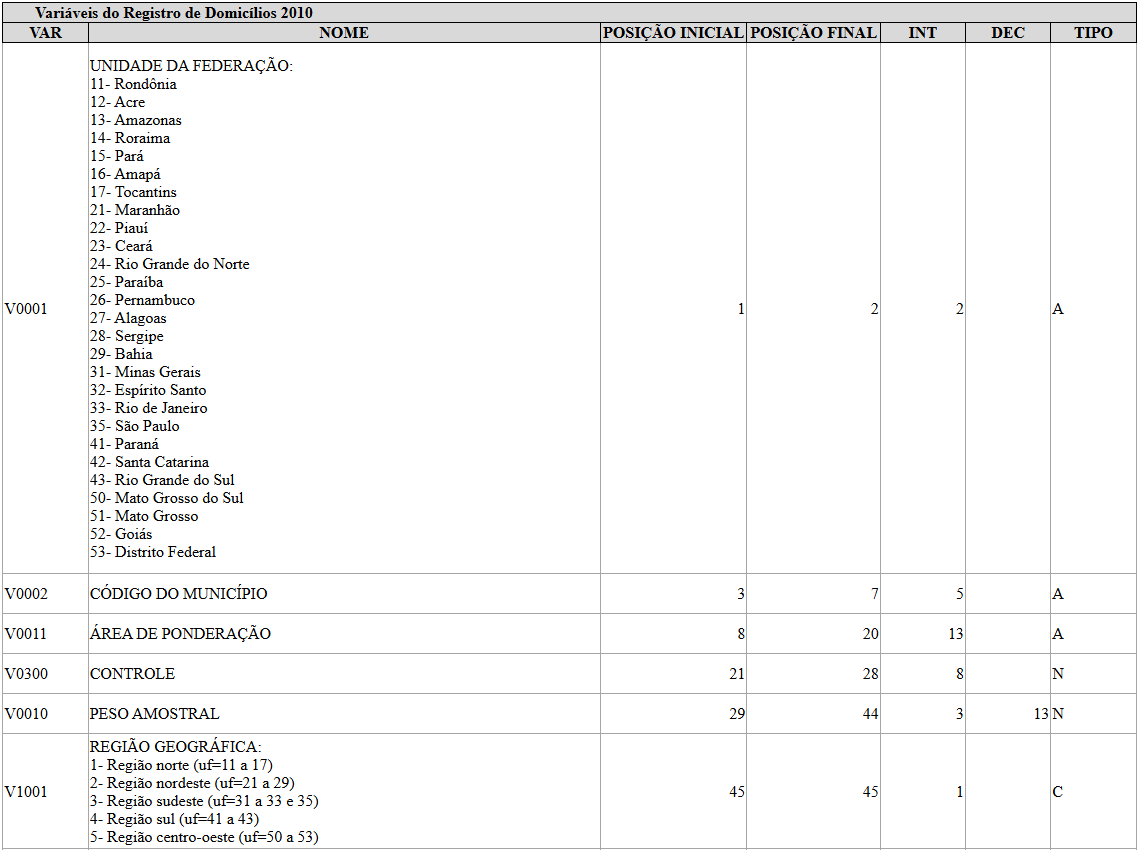
\includegraphics[keepaspectratio]{img/8-microdados/fig-tab_dict.png}}

}

\end{figure}%

Com o dicionário em mãos, o passo seguinte é obter a geometria das áreas
de ponderação de Belo Horizonte (código IBGE 3106200) com a função
\texttt{read\_weighting\_area()} do \texttt{geobr}. Com ele, poderemos
visualizar espacialmente os resultados nos mapas produzidos adiante e
selecionar os códigos das áreas de ponderação a serem utilizados para
filtrar os microdados de BH.

\begin{Shaded}
\begin{Highlighting}[]
\NormalTok{ap\_bh }\OtherTok{\textless{}{-}}\NormalTok{ geobr}\SpecialCharTok{::}\FunctionTok{read\_weighting\_area}\NormalTok{(}
  \AttributeTok{code\_weighting =} \DecValTok{3106200}\NormalTok{,}
  \AttributeTok{year =} \DecValTok{2010}\NormalTok{,}
  \AttributeTok{simplified =} \ConstantTok{FALSE}
\NormalTok{)}

\FunctionTok{ggplot}\NormalTok{(ap\_bh) }\SpecialCharTok{+}
  \FunctionTok{geom\_sf}\NormalTok{(}\AttributeTok{fill =} \StringTok{"gray92"}\NormalTok{, }\AttributeTok{color =} \StringTok{"gray60"}\NormalTok{, }\AttributeTok{linewidth =} \FloatTok{0.3}\NormalTok{) }\SpecialCharTok{+}
  \FunctionTok{theme\_minimal}\NormalTok{() }\SpecialCharTok{+}
  \FunctionTok{labs}\NormalTok{(}\AttributeTok{title =} \ConstantTok{NULL}\NormalTok{)}
\end{Highlighting}
\end{Shaded}

\begin{figure}[H]

\caption{\label{fig-bh-areas}Áreas de ponderação de Belo Horizonte,
Censo Demográfico 2010.}

\centering{

\pandocbounded{
\includegraphics[keepaspectratio]{8-microdados_files/figure-pdf/fig-bh-areas-1.pdf}}

}

\end{figure}%

A partir dos códigos das áreas de ponderação, podemos ler os microdados
filtrados somente para Belo Horizonte. A função
\texttt{read\_households()} do \texttt{censobr} retorna os dados de todo
o Brasil como um \emph{Arrow Table} (assim como na
\texttt{read\_tracts()} para os Agregados por Setor Censitário do
capítulo anterior), sem carregá-los para a memória imediatamente. O
filtro por \texttt{code\_weighting} seleciona apenas os domicílios de
Belo Horizonte, e \texttt{collect()} materializa o resultado em um
\emph{data frame} convencional. Selecionaremos também apenas as
variáveis de interesse, o que reduz consideravelmente o volume de dados
em memória.

\begin{Shaded}
\begin{Highlighting}[]
\DocumentationTok{\#\# Armazenando códigos das áreas de ponderação de BH em um vetor ap\_bh\_cods}
\NormalTok{ap\_bh\_cods }\OtherTok{\textless{}{-}}\NormalTok{ ap\_bh }\SpecialCharTok{|\textgreater{}}
  \FunctionTok{pull}\NormalTok{(code\_weighting)}

\DocumentationTok{\#\# Variáveis selecionadas do arquivo de domicílios}
\NormalTok{cols\_dom }\OtherTok{\textless{}{-}} \FunctionTok{c}\NormalTok{(}
  \StringTok{\textquotesingle{}V0300\textquotesingle{}}\NormalTok{,          }\CommentTok{\# Identificador do domicílio (controle)}
  \StringTok{\textquotesingle{}V0010\textquotesingle{}}\NormalTok{,          }\CommentTok{\# Peso amostral calibrado}
  \StringTok{\textquotesingle{}V1006\textquotesingle{}}\NormalTok{,          }\CommentTok{\# Situação do domicílio (urbano/rural)}
  \StringTok{\textquotesingle{}code\_weighting\textquotesingle{}}\NormalTok{, }\CommentTok{\# Área de ponderação}
  \StringTok{\textquotesingle{}V4001\textquotesingle{}}\NormalTok{,          }\CommentTok{\# Tipo de domicílio}
  \StringTok{\textquotesingle{}V0201\textquotesingle{}}\NormalTok{,          }\CommentTok{\# Condição de ocupação do domicílio (próprio, alugado, ...)}
  \StringTok{\textquotesingle{}V6203\textquotesingle{}}\NormalTok{,          }\CommentTok{\# Densidade (moradores por cômodo)}
  \StringTok{\textquotesingle{}V0207\textquotesingle{}}\NormalTok{,          }\CommentTok{\# Tipo de esgotamento sanitário}
  \StringTok{\textquotesingle{}V6531\textquotesingle{}}\NormalTok{,          }\CommentTok{\# Rendimento domiciliar per capita}
  \StringTok{\textquotesingle{}V0222\textquotesingle{}}           \CommentTok{\# Automóvel particular (sim/não)}
\NormalTok{)}

\DocumentationTok{\#\# Leitura e filtragem para BH}
\NormalTok{md\_dom\_bh }\OtherTok{\textless{}{-}}\NormalTok{ censobr}\SpecialCharTok{::}\FunctionTok{read\_households}\NormalTok{(}\AttributeTok{year =} \DecValTok{2010}\NormalTok{, }\AttributeTok{columns =}\NormalTok{ cols\_dom) }\SpecialCharTok{|\textgreater{}}
  \FunctionTok{filter}\NormalTok{(code\_weighting }\SpecialCharTok{\%in\%}\NormalTok{ ap\_bh\_cods) }\SpecialCharTok{|\textgreater{}}
  \FunctionTok{collect}\NormalTok{()}
\end{Highlighting}
\end{Shaded}

Para visualizar as primeiras linhas dessa base de dados, podemos fazer:

\begin{Shaded}
\begin{Highlighting}[]
\FunctionTok{head}\NormalTok{(md\_dom\_bh)}
\end{Highlighting}
\end{Shaded}

\begin{verbatim}
# A tibble: 6 x 10
  V0300 V0010 V1006 code_weighting V4001 V0201 V6203 V0207 V6531 V0222
  <dbl> <dbl> <chr>          <dbl> <chr> <chr> <dbl> <chr> <dbl> <chr>
1   169  20.7 1      3106200005001 01    1       0.6 1      700  1    
2 14998  23.4 1      3106200005001 01    1       0.8 1      637. 2    
3 32175  20.8 1      3106200005001 01    1       0.9 1      507. 2    
4 43533  19.8 1      3106200005001 01    3       0.6 1      170  2    
5 68172  22.9 1      3106200005001 01    1       0.8 1      333. 1    
6 72256  23.2 1      3106200005001 01    1       1   1      600  2    
\end{verbatim}

Na sequência, faremos a definição do plano amostral que nos permitirá
explorar adequadamente essa base.

\subsection{Declarando o plano
amostral}\label{declarando-o-plano-amostral}

Na Seção~\ref{sec-survey}, mencionamos que para obter estimativas
estatisticamente válidas para os microdados, é preciso declarar ao
\texttt{srvyr} o tipo de amostragem realizada com a função
\texttt{as\_survey\_design}\footnote{No caso do pacote \texttt{survey},
  essa função é a \texttt{svydesign()}}. Sem essa declaração, as
estatísticas descritivas ignorariam a estratificação e os pesos
calibrados, produzindo erros-padrão incorretos e, consequentemente,
intervalos de confiança inadequados.

Lembremos que no caso dos domicílios, temos uma \textbf{amostragem
aleatória estratificada}, em que os setores censitários são os estratos.
Nosso objetivo, então, é caracterizar esse plano amostral por meio do
preenchimento de 4 parâmetros da função \texttt{as\_survey\_design}:

\begin{itemize}
\tightlist
\item
  \texttt{id}: unidade amostral.
\item
  \texttt{strata}: o estrato do plano amostral.
\item
  \texttt{weights}: pesos amostrais.
\item
  \texttt{fpc}: correção de população finita (do inglês, \emph{finite
  population correction}).
\end{itemize}

Em primeiro lugar, para o parâmetro \texttt{id}, devemos indicar as
unidades que foram amostradas aleatoriamente no nosso plano. Como cada
linha representa um domicílio na tabela \texttt{md\_dom\_bh}, podemos
fazer simplesmente passar \texttt{id\ =\ 1} dentro da função
\texttt{as\_survey\_design()}. Na sequência, devemos definir o estrato
do plano amostral em \texttt{strata}. À primeira vista, parece óbvio que
devamos indicar os setores censitários para este parâmetro. Todavia,
além de não haver essa informação nos microdados, lembremos que os pesos
amostrais fornecidos na coluna \texttt{V0010} referem-se à versão
\textbf{calibrada} e que essa calibração é feita no nível da
\textbf{área de ponderação}. Deste modo, devemos inserir a coluna com o
código da área de ponderação da tabela \texttt{md\_dom\_bh}, ou seja,
\texttt{code\_weighting}.

Posteriormente, temos que declarar os pesos, e isto é simples, uma vez
que eles são representados pela coluna \texttt{V0010} de
\texttt{md\_dom\_bh}. Finalmente, precisamos inserir o parâmetro
\texttt{fpc}, um fator usado em amostragem para ajustar a variância, o
erro-padrão e a margem de erro quando a amostra representa uma fração
não desprezível de uma população finita. A ideia é que quando a
população é finita e você retira uma parcela considerável dela, há menos
incerteza do que haveria numa população muito grande ou ``infinita''.
Então, o FPC reduz o erro amostral estimado\footnote{Esse fator é dado
  por \(\sqrt{\frac{N-n}{N-1}}\), em que \(n\) é o tamanho da amostra e
  \(N\) é o tamanho da população}.

Neste caso, o que a função \texttt{as\_survey\_design()} necessita é que
forneçamos uma coluna na base de dados \texttt{md\_dom\_bh} com o total
de unidades correspondente aos estratos definido em \texttt{strata}, ou
seja, a quantidade de domicílios total da área de ponderação (no nosso
caso.) Uma maneira de obtermos essa informação é somar os valores dos
pesos \texttt{V0010} em cada área de ponderação. Lembre-se que a ideia
do peso de uma unidade amostral é exatamente indicar quantas unidades
ela representa em seu estrato. Logo somar os pesos de todas as unidades
dentro da área de ponderação corresponderá ao valor total de domicílios
nesta área.

Para tanto, devemos primeiro produzimos uma tabela sumarizada que
computa os totais de domicílios de cada área de ponderação. Na
sequência, trazemos esses totais da tabela sumarizada para cada linha de
\texttt{md\_dom\_bh} com o operador \texttt{left\_join}, informando
\texttt{code\_weighting} como chave, conforme o código abaixo:

\begin{Shaded}
\begin{Highlighting}[]
\DocumentationTok{\#\# Total de domicílios expandido por área de ponderação (para correção de população finita)}
\NormalTok{dom\_ap }\OtherTok{\textless{}{-}}\NormalTok{ md\_dom\_bh }\SpecialCharTok{|\textgreater{}}
  \FunctionTok{group\_by}\NormalTok{(code\_weighting) }\SpecialCharTok{|\textgreater{}}
  \FunctionTok{summarize}\NormalTok{(}\AttributeTok{n\_dom =} \FunctionTok{sum}\NormalTok{(V0010))}

\DocumentationTok{\#\# Adiciona n\_dom ao arquivo de domicílios}
\NormalTok{md\_dom\_bh }\OtherTok{\textless{}{-}}\NormalTok{ md\_dom\_bh }\SpecialCharTok{|\textgreater{}}
  \FunctionTok{left\_join}\NormalTok{(dom\_ap, }\AttributeTok{by =} \StringTok{"code\_weighting"}\NormalTok{)}

\DocumentationTok{\#\# Observe a última coluna n\_dom adicionada à tabela}
\FunctionTok{head}\NormalTok{(md\_dom\_bh)}
\end{Highlighting}
\end{Shaded}

\begin{verbatim}
# A tibble: 6 x 11
  V0300 V0010 V1006 code_weighting V4001 V0201 V6203 V0207 V6531 V0222 n_dom
  <dbl> <dbl> <chr>          <dbl> <chr> <chr> <dbl> <chr> <dbl> <chr> <dbl>
1   169  20.7 1      3106200005001 01    1       0.6 1      700  1     13998
2 14998  23.4 1      3106200005001 01    1       0.8 1      637. 2     13998
3 32175  20.8 1      3106200005001 01    1       0.9 1      507. 2     13998
4 43533  19.8 1      3106200005001 01    3       0.6 1      170  2     13998
5 68172  22.9 1      3106200005001 01    1       0.8 1      333. 1     13998
6 72256  23.2 1      3106200005001 01    1       1   1      600  2     13998
\end{verbatim}

Observe que os valores de \texttt{n\_dom} são repetidos para todas as 6
primeiras linhas mostradas acima, pois essas observações são relativas a
domicílios de uma mesma área de ponderação identificada pela coluna
\texttt{code\_weighting}. Com estas definições, podemos finalmente
produzir o plano amostral da função \texttt{as\_survey\_design()}, de
acordo com o código abaixo:

\begin{Shaded}
\begin{Highlighting}[]
\DocumentationTok{\#\# Objeto de desenho amostral (srvyr)}
\NormalTok{pa\_dom }\OtherTok{\textless{}{-}}\NormalTok{ md\_dom\_bh }\SpecialCharTok{|\textgreater{}}
  \FunctionTok{as\_survey\_design}\NormalTok{(}
    \AttributeTok{ids     =} \DecValTok{1}\NormalTok{,               }\CommentTok{\# cada linha é um domicílio (unidade sorteada)}
    \AttributeTok{strata  =}\NormalTok{ code\_weighting,  }\CommentTok{\# estratos = áreas de ponderação (onde a calibração foi feita)}
    \AttributeTok{weights =}\NormalTok{ V0010,           }\CommentTok{\# pesos calibrados}
    \AttributeTok{fpc     =}\NormalTok{ n\_dom            }\CommentTok{\# total de domicílios em cada área (correção de população finita)}
\NormalTok{  )}
\end{Highlighting}
\end{Shaded}

O objeto \texttt{pa\_dom} reúne os dados e a especificação completa do
plano amostral. Todas as funções de análise do \texttt{srvyr} a seguir
receberão esse objeto, garantindo que as estimativas levem em conta a
estratificação e os pesos.

\subsection{Calculando estatísticas}\label{sec-dom-estat}

Com o plano amostral configurado, podemos calcular estimativas para
qualquer variável dos microdados. O fluxo de trabalho é similar ao do
\texttt{dplyr}, com \texttt{summarize()} para estatísticas do município
como um todo e \texttt{group\_by()} para análises por subgrupos.

Começamos estimando a média e a mediana do rendimento domiciliar per
capita (\texttt{V6531}) em Belo Horizonte. Os argumentos
\texttt{vartype\ =\ "ci"} (de \emph{Confidence Interval}) e
\texttt{level\ =\ 0.95} solicitam que o resultado inclua os limites
inferior e superior do intervalo de confiança de 95\%.

\begin{Shaded}
\begin{Highlighting}[]
\NormalTok{pa\_dom }\SpecialCharTok{|\textgreater{}}
  \FunctionTok{summarize}\NormalTok{(}
    \AttributeTok{renda\_media   =} \FunctionTok{survey\_mean}\NormalTok{(V6531, }\AttributeTok{na.rm =} \ConstantTok{TRUE}\NormalTok{,}
                                \AttributeTok{vartype =} \StringTok{"ci"}\NormalTok{, }\AttributeTok{level =} \FloatTok{0.95}\NormalTok{),}
    \AttributeTok{renda\_mediana =} \FunctionTok{survey\_median}\NormalTok{(V6531, }\AttributeTok{na.rm =} \ConstantTok{TRUE}\NormalTok{,}
                                  \AttributeTok{vartype =} \StringTok{"ci"}\NormalTok{, }\AttributeTok{level =} \FloatTok{0.95}\NormalTok{)}
\NormalTok{  ) }\SpecialCharTok{|\textgreater{}}
\NormalTok{  knitr}\SpecialCharTok{::}\FunctionTok{kable}\NormalTok{(}
    \AttributeTok{col.names =} \FunctionTok{c}\NormalTok{(}\StringTok{"Média"}\NormalTok{, }\StringTok{"IC inf. (média)"}\NormalTok{, }\StringTok{"IC sup. (média)"}\NormalTok{,}
                  \StringTok{"Mediana"}\NormalTok{, }\StringTok{"IC inf. (mediana)"}\NormalTok{, }\StringTok{"IC sup. (mediana)"}\NormalTok{),}
    \AttributeTok{digits =} \DecValTok{1}
\NormalTok{  )}
\end{Highlighting}
\end{Shaded}

{

\begin{longtable}[]{@{}
  >{\raggedleft\arraybackslash}p{(\linewidth - 10\tabcolsep) * \real{0.0843}}
  >{\raggedleft\arraybackslash}p{(\linewidth - 10\tabcolsep) * \real{0.1928}}
  >{\raggedleft\arraybackslash}p{(\linewidth - 10\tabcolsep) * \real{0.1928}}
  >{\raggedleft\arraybackslash}p{(\linewidth - 10\tabcolsep) * \real{0.0964}}
  >{\raggedleft\arraybackslash}p{(\linewidth - 10\tabcolsep) * \real{0.2169}}
  >{\raggedleft\arraybackslash}p{(\linewidth - 10\tabcolsep) * \real{0.2169}}@{}}

\caption{\label{tbl-renda-bh}Rendimento domiciliar per capita em Belo
Horizonte (R\$), Censo 2010.}

\tabularnewline

\toprule\noalign{}
\begin{minipage}[b]{\linewidth}\raggedleft
Média
\end{minipage} & \begin{minipage}[b]{\linewidth}\raggedleft
IC inf. (média)
\end{minipage} & \begin{minipage}[b]{\linewidth}\raggedleft
IC sup. (média)
\end{minipage} & \begin{minipage}[b]{\linewidth}\raggedleft
Mediana
\end{minipage} & \begin{minipage}[b]{\linewidth}\raggedleft
IC inf. (mediana)
\end{minipage} & \begin{minipage}[b]{\linewidth}\raggedleft
IC sup. (mediana)
\end{minipage} \\
\midrule\noalign{}
\endhead
\bottomrule\noalign{}
\endlastfoot
1765.2 & 1714.5 & 1815.8 & 765 & 759 & 777.5 \\

\end{longtable}

}

A mediana é substancialmente menor que a média, o que reflete a
assimetria positiva da distribuição de renda. Uma minoria de domicílios
com rendimentos muito altos eleva a média sem deslocar a mediana,
tornando esta última a medida mais representativa da renda típica.

Uma comparação natural é verificar como a posse de automóvel particular
(\texttt{V0222}) se associa ao rendimento domiciliar (\texttt{V6531}). O
gráfico a seguir apresenta a renda mediana estimada para cada categoria
(função \texttt{survey\_median()}), com o respectivo intervalo de
confiança de 95\%.

\begin{Shaded}
\begin{Highlighting}[]
\NormalTok{pa\_dom }\SpecialCharTok{|\textgreater{}}
  \FunctionTok{filter}\NormalTok{(}\SpecialCharTok{!}\FunctionTok{is.na}\NormalTok{(V0222)) }\SpecialCharTok{|\textgreater{}}
  \FunctionTok{group\_by}\NormalTok{(V0222) }\SpecialCharTok{|\textgreater{}}
  \FunctionTok{summarize}\NormalTok{(}
    \AttributeTok{renda\_mediana =} \FunctionTok{survey\_median}\NormalTok{(V6531, }\AttributeTok{na.rm =} \ConstantTok{TRUE}\NormalTok{,}
                                  \AttributeTok{vartype =} \StringTok{"ci"}\NormalTok{, }\AttributeTok{level =} \FloatTok{0.95}\NormalTok{)}
\NormalTok{  ) }\SpecialCharTok{|\textgreater{}}
  \FunctionTok{mutate}\NormalTok{(}\AttributeTok{V0222 =} \FunctionTok{factor}\NormalTok{(V0222,}
                        \AttributeTok{levels =} \FunctionTok{c}\NormalTok{(}\StringTok{"1"}\NormalTok{, }\StringTok{"2"}\NormalTok{),}
                        \AttributeTok{labels =} \FunctionTok{c}\NormalTok{(}\StringTok{"Com automóvel"}\NormalTok{, }\StringTok{"Sem automóvel"}\NormalTok{))) }\SpecialCharTok{|\textgreater{}}
  \FunctionTok{ggplot}\NormalTok{(}\FunctionTok{aes}\NormalTok{(}\AttributeTok{x =}\NormalTok{ V0222, }\AttributeTok{y =}\NormalTok{ renda\_mediana,}
             \AttributeTok{ymin =}\NormalTok{ renda\_mediana\_low, }\AttributeTok{ymax =}\NormalTok{ renda\_mediana\_upp)) }\SpecialCharTok{+}
  \FunctionTok{geom\_col}\NormalTok{(}\AttributeTok{fill =} \StringTok{"steelblue"}\NormalTok{, }\AttributeTok{alpha =} \FloatTok{0.85}\NormalTok{, }\AttributeTok{width =} \FloatTok{0.5}\NormalTok{) }\SpecialCharTok{+}
  \FunctionTok{geom\_errorbar}\NormalTok{(}\AttributeTok{width =} \FloatTok{0.15}\NormalTok{, }\AttributeTok{color =} \StringTok{"orange"}\NormalTok{, }\AttributeTok{linewidth =} \FloatTok{0.8}\NormalTok{) }\SpecialCharTok{+}
  \FunctionTok{scale\_y\_continuous}\NormalTok{(}
    \AttributeTok{labels =}\NormalTok{ scales}\SpecialCharTok{::}\FunctionTok{label\_dollar}\NormalTok{(}\AttributeTok{prefix =} \StringTok{"R$ "}\NormalTok{, }\AttributeTok{big.mark =} \StringTok{"."}\NormalTok{, }\AttributeTok{decimal.mark =} \StringTok{","}\NormalTok{)}
\NormalTok{  ) }\SpecialCharTok{+}
  \FunctionTok{labs}\NormalTok{(}\AttributeTok{x =} \ConstantTok{NULL}\NormalTok{, }\AttributeTok{y =} \StringTok{"Renda mediana (R$)"}\NormalTok{) }\SpecialCharTok{+}
  \FunctionTok{theme\_minimal}\NormalTok{()}
\end{Highlighting}
\end{Shaded}

\begin{figure}[H]

\caption{\label{fig-renda-automovel}Rendimento domiciliar per capita
mediano por posse de automóvel, Belo Horizonte (Censo 2010). Barras de
erro indicam IC 95\%.}

\centering{

\pandocbounded{
\includegraphics[keepaspectratio]{8-microdados_files/figure-pdf/fig-renda-automovel-1.pdf}}

}

\end{figure}%

A diferença entre os dois grupos é expressiva, e como os intervalos de
confiança não se sobrepõem, ela é estatisticamente significativa.
Domicílios com automóvel apresentam renda per capita mediana
substancialmente maior, resultado esperado dado o custo de aquisição e
manutenção de um veículo próprio.

Os microdados também permitem estimar proporções para variáveis
categóricas. O gráfico a seguir apresenta a distribuição de domicílios
por condição de ocupação do domicílio (\texttt{V0201}), com a proporção
estimada e o intervalo de confiança de 95\% para cada categoria (função
\texttt{survey\_prop()}).

\begin{Shaded}
\begin{Highlighting}[]
\NormalTok{pa\_dom }\SpecialCharTok{|\textgreater{}}
  \FunctionTok{group\_by}\NormalTok{(V0201) }\SpecialCharTok{|\textgreater{}}
  \FunctionTok{summarize}\NormalTok{(}
    \AttributeTok{proporcao =} \FunctionTok{survey\_prop}\NormalTok{(}\AttributeTok{vartype =} \StringTok{"ci"}\NormalTok{, }\AttributeTok{level =} \FloatTok{0.95}\NormalTok{)}
\NormalTok{  ) }\SpecialCharTok{|\textgreater{}}
  \FunctionTok{mutate}\NormalTok{(}\AttributeTok{V0201 =} \FunctionTok{factor}\NormalTok{(V0201,}
                        \AttributeTok{levels =} \FunctionTok{c}\NormalTok{(}\StringTok{"1"}\NormalTok{, }\StringTok{"2"}\NormalTok{,}\StringTok{"3"}\NormalTok{,}\StringTok{"4"}\NormalTok{,}\StringTok{"5"}\NormalTok{,}\StringTok{"6"}\NormalTok{),}
                        \AttributeTok{labels =} \FunctionTok{c}\NormalTok{(}\StringTok{"Próprio de algum morador {-} já pago"}\NormalTok{, }\StringTok{"Próprio de algum morador {-} ainda pagando"}\NormalTok{,}
                                   \StringTok{"Alugado"}\NormalTok{,}\StringTok{"Cedido por empregador"}\NormalTok{,}\StringTok{"Cedido de outra forma"}\NormalTok{,}\StringTok{"Outra condição"}\NormalTok{)}
\NormalTok{                        )}
\NormalTok{         ) }\SpecialCharTok{|\textgreater{}} 
  \FunctionTok{ggplot}\NormalTok{(}\FunctionTok{aes}\NormalTok{(}\AttributeTok{x =} \FunctionTok{reorder}\NormalTok{(V0201, proporcao), }\AttributeTok{y =}\NormalTok{ proporcao,}
             \AttributeTok{ymin =}\NormalTok{ proporcao\_low, }\AttributeTok{ymax =}\NormalTok{ proporcao\_upp)) }\SpecialCharTok{+}
  \FunctionTok{geom\_col}\NormalTok{(}\AttributeTok{fill =} \StringTok{"steelblue"}\NormalTok{, }\AttributeTok{alpha =} \FloatTok{0.85}\NormalTok{) }\SpecialCharTok{+}
  \FunctionTok{geom\_errorbar}\NormalTok{(}\AttributeTok{width =} \FloatTok{0.3}\NormalTok{, }\AttributeTok{color =} \StringTok{"orange"}\NormalTok{, }\AttributeTok{linewidth =} \FloatTok{0.8}\NormalTok{) }\SpecialCharTok{+}
  \FunctionTok{coord\_flip}\NormalTok{() }\SpecialCharTok{+}
  \FunctionTok{scale\_y\_continuous}\NormalTok{(}\AttributeTok{labels =}\NormalTok{ scales}\SpecialCharTok{::}\FunctionTok{label\_percent}\NormalTok{(}\AttributeTok{decimal.mark =} \StringTok{","}\NormalTok{)) }\SpecialCharTok{+}
  \FunctionTok{labs}\NormalTok{(}\AttributeTok{x =} \ConstantTok{NULL}\NormalTok{, }\AttributeTok{y =} \StringTok{"Proporção"}\NormalTok{) }\SpecialCharTok{+}
  \FunctionTok{theme\_minimal}\NormalTok{()}
\end{Highlighting}
\end{Shaded}

\begin{figure}[H]

\caption{\label{fig-condicao-ocup}Proporção de domicílios por condição
de ocupação, Belo Horizonte (Censo 2010). Barras de erro indicam IC
95\%.}

\centering{

\pandocbounded{
\includegraphics[keepaspectratio]{8-microdados_files/figure-pdf/fig-condicao-ocup-1.pdf}}

}

\end{figure}%

Por fim, vamos mostrar como produzir uma nova variável a partir de uma
existente e computar algumas estatísticas. Utilizaremos a variável
\texttt{V0207} (Tipo de esgotamento sanitário), cujas cateorias são: -
1- Rede geral de esgoto ou pluvial - 2- Fossa séptica - 3- Fossa
rudimentar - 4- Vala - 5- Rio, lago ou mar - 6- Outro

Produziremos uma nova variável denominada \texttt{esg\_rede} que agrupa
as seis categorias em duas, separando os domicílios ligados à rede geral
de esgoto ou pluvial e os que usam fossa séptica (categorias 1 e 2)
daqueles que destinam o esgoto de outras formas (categorias 3 a 6). O
agrupamento é uma simplificação de trabalho, e os critérios técnicos que
sustentam essa separação serão discutidos na Parte 3 do livro.

\begin{Shaded}
\begin{Highlighting}[]
\NormalTok{pa\_dom }\SpecialCharTok{|\textgreater{}}
  \FunctionTok{mutate}\NormalTok{(}\AttributeTok{esg\_rede =} \FunctionTok{factor}\NormalTok{(}\FunctionTok{ifelse}\NormalTok{(V0207 }\SpecialCharTok{\%in\%} \FunctionTok{c}\NormalTok{(}\StringTok{\textquotesingle{}1\textquotesingle{}}\NormalTok{,}\StringTok{\textquotesingle{}2\textquotesingle{}}\NormalTok{), }\StringTok{\textquotesingle{}Rede ou fossa\textquotesingle{}}\NormalTok{, }\StringTok{\textquotesingle{}Outras formas\textquotesingle{}}\NormalTok{))) }\SpecialCharTok{|\textgreater{}}
  \FunctionTok{group\_by}\NormalTok{(esg\_rede) }\SpecialCharTok{|\textgreater{}}
  \FunctionTok{summarize}\NormalTok{(}\AttributeTok{proporcao =} \FunctionTok{survey\_prop}\NormalTok{(}\AttributeTok{vartype =} \StringTok{"ci"}\NormalTok{, }\AttributeTok{level =} \FloatTok{0.95}\NormalTok{)) }\SpecialCharTok{|\textgreater{}}
  \FunctionTok{ggplot}\NormalTok{(}\FunctionTok{aes}\NormalTok{(}\AttributeTok{x =}\NormalTok{ esg\_rede, }\AttributeTok{y =}\NormalTok{ proporcao,}
             \AttributeTok{ymin =}\NormalTok{ proporcao\_low, }\AttributeTok{ymax =}\NormalTok{ proporcao\_upp)) }\SpecialCharTok{+}
  \FunctionTok{geom\_col}\NormalTok{(}\AttributeTok{fill =} \StringTok{"steelblue"}\NormalTok{, }\AttributeTok{alpha =} \FloatTok{0.85}\NormalTok{, }\AttributeTok{width =} \FloatTok{0.5}\NormalTok{) }\SpecialCharTok{+}
  \FunctionTok{geom\_errorbar}\NormalTok{(}\AttributeTok{width =} \FloatTok{0.15}\NormalTok{, }\AttributeTok{color =} \StringTok{"orange"}\NormalTok{, }\AttributeTok{linewidth =} \FloatTok{0.8}\NormalTok{) }\SpecialCharTok{+}
  \FunctionTok{scale\_y\_continuous}\NormalTok{(}\AttributeTok{labels =}\NormalTok{ scales}\SpecialCharTok{::}\FunctionTok{label\_percent}\NormalTok{(}\AttributeTok{decimal.mark =} \StringTok{","}\NormalTok{)) }\SpecialCharTok{+}
  \FunctionTok{labs}\NormalTok{(}\AttributeTok{x =} \ConstantTok{NULL}\NormalTok{, }\AttributeTok{y =} \StringTok{"Proporção"}\NormalTok{) }\SpecialCharTok{+}
  \FunctionTok{theme\_minimal}\NormalTok{()}
\end{Highlighting}
\end{Shaded}

\begin{figure}[H]

\caption{\label{fig-esgoto-bh}Proporção de domicílios por tipo de
esgotamento sanitário, Belo Horizonte (Censo 2010). Barras de erro
indicam IC 95\%.}

\centering{

\pandocbounded{
\includegraphics[keepaspectratio]{8-microdados_files/figure-pdf/fig-esgoto-bh-1.pdf}}

}

\end{figure}%

\subsection{Produzindo mapas}\label{produzindo-mapas}

As mesmas estatísticas calculadas para o município como um todo podem
ser desagregadas por área de ponderação com
\texttt{group\_by(code\_weighting)} e visualizadas espacialmente com
\texttt{geom\_sf()}. O mapa da Figura~\ref{fig-bh-renda} apresenta a
renda domiciliar per capita mediana em cada área de ponderação. Para
isso, calculamos a mediana por área com \texttt{survey\_median()} e
depois unimos o resultado à geometria com \texttt{left\_join()}.

\begin{Shaded}
\begin{Highlighting}[]
\DocumentationTok{\#\# Estatística por área de ponderação}
\NormalTok{rend\_ap }\OtherTok{\textless{}{-}}\NormalTok{ pa\_dom }\SpecialCharTok{|\textgreater{}}
  \FunctionTok{group\_by}\NormalTok{(code\_weighting) }\SpecialCharTok{|\textgreater{}}
  \FunctionTok{summarize}\NormalTok{(}\AttributeTok{rend\_mediana =} \FunctionTok{survey\_median}\NormalTok{(V6531, }\AttributeTok{na.rm =} \ConstantTok{TRUE}\NormalTok{))}

\DocumentationTok{\#\# Join com geometria e mapa}
\NormalTok{ap\_bh }\SpecialCharTok{|\textgreater{}}
  \FunctionTok{left\_join}\NormalTok{(rend\_ap, }\AttributeTok{by =} \FunctionTok{join\_by}\NormalTok{(code\_weighting)) }\SpecialCharTok{|\textgreater{}}
  \FunctionTok{ggplot}\NormalTok{() }\SpecialCharTok{+}
  \FunctionTok{geom\_sf}\NormalTok{(}\FunctionTok{aes}\NormalTok{(}\AttributeTok{fill =}\NormalTok{ rend\_mediana), }\AttributeTok{color =} \StringTok{"white"}\NormalTok{, }\AttributeTok{linewidth =} \FloatTok{0.2}\NormalTok{) }\SpecialCharTok{+}
  \FunctionTok{scale\_fill\_distiller}\NormalTok{(}
    \AttributeTok{palette =} \StringTok{"RdYlGn"}\NormalTok{,}
    \AttributeTok{direction =} \DecValTok{1}\NormalTok{,}
    \AttributeTok{name =} \StringTok{"Renda mediana}\SpecialCharTok{\textbackslash{}n}\StringTok{(R$)"}\NormalTok{,}
    \AttributeTok{labels =}\NormalTok{ scales}\SpecialCharTok{::}\FunctionTok{label\_dollar}\NormalTok{(}\AttributeTok{prefix =} \StringTok{"R$ "}\NormalTok{, }\AttributeTok{big.mark =} \StringTok{"."}\NormalTok{, }\AttributeTok{decimal.mark =} \StringTok{","}\NormalTok{)}
\NormalTok{  ) }\SpecialCharTok{+}
  \FunctionTok{theme\_minimal}\NormalTok{() }\SpecialCharTok{+}
  \FunctionTok{theme}\NormalTok{(}
    \AttributeTok{axis.text =} \FunctionTok{element\_blank}\NormalTok{(),}
    \AttributeTok{axis.ticks =} \FunctionTok{element\_blank}\NormalTok{(),}
    \AttributeTok{panel.grid =} \FunctionTok{element\_blank}\NormalTok{()}
\NormalTok{  )}
\end{Highlighting}
\end{Shaded}

\begin{figure}[H]

\caption{\label{fig-bh-renda}Rendimento domiciliar per capita mediano
por área de ponderação, Belo Horizonte (Censo 2010, R\$ de julho de
2010).}

\centering{

\pandocbounded{
\includegraphics[keepaspectratio]{8-microdados_files/figure-pdf/fig-bh-renda-1.pdf}}

}

\end{figure}%

O padrão espacial é marcante, com áreas com rendimentos mais altos
concentrando-se na região sudeste do município, enquanto os menores
rendimentos predominam em regiões mais periféricas ao Sul e ao Norte. O
mapa da Figura~\ref{fig-bh-esgoto} apresenta, para as mesmas unidades
espaciais, a proporção de domicílios com esgotamento por rede geral ou
fossa séptica. O procedimento é idêntico ao do mapa anterior,
substituindo \texttt{survey\_median()} por \texttt{survey\_prop()} e
criando uma variável indicadora antes do agrupamento.

\begin{Shaded}
\begin{Highlighting}[]
\DocumentationTok{\#\# Estatística por área de ponderação}
\NormalTok{esg\_ap }\OtherTok{\textless{}{-}}\NormalTok{ pa\_dom }\SpecialCharTok{|\textgreater{}}
  \FunctionTok{mutate}\NormalTok{(}\AttributeTok{esg\_rede =} \FunctionTok{factor}\NormalTok{(}\FunctionTok{ifelse}\NormalTok{(V0207 }\SpecialCharTok{\%in\%} \FunctionTok{c}\NormalTok{(}\StringTok{\textquotesingle{}1\textquotesingle{}}\NormalTok{,}\StringTok{\textquotesingle{}2\textquotesingle{}}\NormalTok{), }\StringTok{\textquotesingle{}Rede ou fossa\textquotesingle{}}\NormalTok{, }\StringTok{\textquotesingle{}Outras formas\textquotesingle{}}\NormalTok{))) }\SpecialCharTok{|\textgreater{}} 
  \FunctionTok{group\_by}\NormalTok{(code\_weighting, esg\_rede) }\SpecialCharTok{|\textgreater{}}
  \FunctionTok{summarize}\NormalTok{(}\AttributeTok{proporcao =} \FunctionTok{survey\_prop}\NormalTok{()) }\SpecialCharTok{|\textgreater{}}
  \FunctionTok{filter}\NormalTok{(esg\_rede }\SpecialCharTok{==} \StringTok{\textquotesingle{}Rede ou fossa\textquotesingle{}}\NormalTok{)}

\DocumentationTok{\#\# Join com geometria e mapa}
\NormalTok{ap\_bh }\SpecialCharTok{|\textgreater{}}
  \FunctionTok{left\_join}\NormalTok{(esg\_ap, }\AttributeTok{by =} \FunctionTok{join\_by}\NormalTok{(code\_weighting)) }\SpecialCharTok{|\textgreater{}}
  \FunctionTok{ggplot}\NormalTok{() }\SpecialCharTok{+}
  \FunctionTok{geom\_sf}\NormalTok{(}\FunctionTok{aes}\NormalTok{(}\AttributeTok{fill =}\NormalTok{ proporcao), }\AttributeTok{color =} \StringTok{"white"}\NormalTok{, }\AttributeTok{linewidth =} \FloatTok{0.2}\NormalTok{) }\SpecialCharTok{+}
  \FunctionTok{scale\_fill\_distiller}\NormalTok{(}
    \AttributeTok{palette =} \StringTok{"Blues"}\NormalTok{,}
    \AttributeTok{direction =} \DecValTok{1}\NormalTok{,}
    \AttributeTok{name =} \StringTok{"Proporção com}\SpecialCharTok{\textbackslash{}n}\StringTok{rede ou fossa"}\NormalTok{,}
    \AttributeTok{labels =}\NormalTok{ scales}\SpecialCharTok{::}\FunctionTok{label\_percent}\NormalTok{(}\AttributeTok{decimal.mark =} \StringTok{","}\NormalTok{)}
\NormalTok{  ) }\SpecialCharTok{+}
  \FunctionTok{theme\_minimal}\NormalTok{() }\SpecialCharTok{+}
  \FunctionTok{theme}\NormalTok{(}
    \AttributeTok{axis.text =} \FunctionTok{element\_blank}\NormalTok{(),}
    \AttributeTok{axis.ticks =} \FunctionTok{element\_blank}\NormalTok{(),}
    \AttributeTok{panel.grid =} \FunctionTok{element\_blank}\NormalTok{()}
\NormalTok{  )}
\end{Highlighting}
\end{Shaded}

\begin{figure}[H]

\caption{\label{fig-bh-esgoto}Proporção de domicílios com esgotamento
por rede geral, rede pluvial ou fossa séptica, por área de ponderação,
Belo Horizonte (Censo 2010).}

\centering{

\pandocbounded{
\includegraphics[keepaspectratio]{8-microdados_files/figure-pdf/fig-bh-esgoto-1.pdf}}

}

\end{figure}%

Comparando os dois mapas, observa-se uma associação positiva entre renda
e cobertura de saneamento. As áreas com maior rendimento tendem a
apresentar maior proporção de domicílios atendidos pela rede geral de
esgoto. A relação, contudo, não é perfeita, e identificar onde o
saneamento está aquém do esperado dado o nível de renda é exatamente o
tipo de diagnóstico que os microdados da amostra viabilizam.

\section{\texorpdfstring{Analisando microdados de
\emph{indivíduos}}{Analisando microdados de indivíduos}}\label{sec-ind}

\subsection{Obtendo e preparando os
dados}\label{obtendo-e-preparando-os-dados-1}

O arquivo de pessoas do Censo segue a mesma lógica de acesso que o de
domicílios, mas exige atenção especial na especificação do plano
amostral. Como discutido na Seção~\ref{sec-survey}, os indivíduos não
foram sorteados diretamente. O que foi sorteado foi o domicílio, e todos
os seus moradores foram entrevistados. Essa estrutura de
\textbf{amostragem estratificada e conglomerada} precisa ser declarada
explicitamente, como veremos adiante.

Assim como no arquivo de domicílios, vale consultar o dicionário antes
de iniciar a leitura.

\begin{Shaded}
\begin{Highlighting}[]
\NormalTok{censobr}\SpecialCharTok{::}\FunctionTok{data\_dictionary}\NormalTok{(}\AttributeTok{year =} \DecValTok{2010}\NormalTok{, }\AttributeTok{dataset =} \StringTok{\textquotesingle{}population\textquotesingle{}}\NormalTok{)}
\end{Highlighting}
\end{Shaded}

O código a seguir seleciona as variáveis de interesse e lê os microdados
de indivíduos de Belo Horizonte, aproveitando os códigos de área de
ponderação já extraídos anteriormente.

\begin{Shaded}
\begin{Highlighting}[]
\DocumentationTok{\#\# Variáveis selecionadas do arquivo de pessoas}
\NormalTok{cols\_ind }\OtherTok{\textless{}{-}} \FunctionTok{c}\NormalTok{(}
  \StringTok{\textquotesingle{}V0300\textquotesingle{}}\NormalTok{,          }\CommentTok{\# Identificador do domicílio (controle, usado como id do conglomerado)}
  \StringTok{\textquotesingle{}V0010\textquotesingle{}}\NormalTok{,          }\CommentTok{\# Peso amostral calibrado}
  \StringTok{\textquotesingle{}V1006\textquotesingle{}}\NormalTok{,          }\CommentTok{\# Situação do domicílio (urbano/rural)}
  \StringTok{\textquotesingle{}code\_weighting\textquotesingle{}}\NormalTok{, }\CommentTok{\# Área de ponderação}
  \StringTok{\textquotesingle{}V0601\textquotesingle{}}\NormalTok{,          }\CommentTok{\# Sexo}
  \StringTok{\textquotesingle{}V0606\textquotesingle{}}\NormalTok{,          }\CommentTok{\# Cor ou raça}
  \StringTok{\textquotesingle{}V6036\textquotesingle{}}\NormalTok{,          }\CommentTok{\# Idade (em anos)}
  \StringTok{\textquotesingle{}V6400\textquotesingle{}}\NormalTok{,          }\CommentTok{\# Nível de instrução}
  \StringTok{\textquotesingle{}V0661\textquotesingle{}}\NormalTok{,          }\CommentTok{\# Retorna do trabalho para casa diariamente?}
  \StringTok{\textquotesingle{}V0662\textquotesingle{}}           \CommentTok{\# Tempo habitual de deslocamento até o trabalho}
\NormalTok{)}

\DocumentationTok{\#\# Leitura e filtragem para BH}
\NormalTok{md\_ind\_bh }\OtherTok{\textless{}{-}}\NormalTok{ censobr}\SpecialCharTok{::}\FunctionTok{read\_population}\NormalTok{(}\AttributeTok{year =} \DecValTok{2010}\NormalTok{, }\AttributeTok{columns =}\NormalTok{ cols\_ind) }\SpecialCharTok{|\textgreater{}}
  \FunctionTok{filter}\NormalTok{(code\_weighting }\SpecialCharTok{\%in\%}\NormalTok{ ap\_bh\_cods) }\SpecialCharTok{|\textgreater{}}
  \FunctionTok{collect}\NormalTok{()}
\end{Highlighting}
\end{Shaded}

\subsection{Declarando o plano
amostral}\label{declarando-o-plano-amostral-1}

O plano amostral de indivíduos difere do de domicílios em um aspecto
fundamental, que é a declaração da conglomeração. No arquivo de pessoas,
os moradores não chegaram à amostra de forma independente. Foram os
domicílios que foram sorteados, e cada morador pertence a um
conglomerado (seu domicílio). Dois moradores do mesmo domicílio tendem a
ter características muito mais similares entre si do que dois indivíduos
escolhidos ao acaso na população. Ignorar essa estrutura leva a
erros-padrão subestimados, porque o \texttt{srvyr} contaria cada
observação como se fosse independente, quando na verdade membros de uma
mesma família contribuem com informação redundante.

Para informar a conglomeração ao \texttt{srvyr}, usamos o argumento
\texttt{ids\ =\ V0300}, em que \texttt{V0300} é o identificador do
domicílio. Lembre-se que o argumento \texttt{ids} espera a unidade
amostral sorteada que, no nosso caso, são os domicílios. Com isso, o
pacote entende que todos os indivíduos com o mesmo \texttt{V0300} foram
coletados juntos, como parte do mesmo conglomerado. Além disso, o
\texttt{fpc} agora passa a ser o total expandido de pessoas por área de
ponderação, conforme o código abaixo:

\begin{Shaded}
\begin{Highlighting}[]
\DocumentationTok{\#\# Total de indivíduos expandido por área de ponderação (para correção de finitude)}
\NormalTok{pop\_ap }\OtherTok{\textless{}{-}}\NormalTok{ md\_ind\_bh }\SpecialCharTok{|\textgreater{}}
  \FunctionTok{group\_by}\NormalTok{(code\_weighting) }\SpecialCharTok{|\textgreater{}}
  \FunctionTok{summarize}\NormalTok{(}\AttributeTok{n\_ind =} \FunctionTok{sum}\NormalTok{(V0010))}

\DocumentationTok{\#\# Adiciona n\_ind ao arquivo de pessoas}
\NormalTok{md\_ind\_bh }\OtherTok{\textless{}{-}}\NormalTok{ md\_ind\_bh }\SpecialCharTok{|\textgreater{}}
  \FunctionTok{left\_join}\NormalTok{(pop\_ap, }\AttributeTok{by =} \FunctionTok{join\_by}\NormalTok{(code\_weighting))}

\DocumentationTok{\#\# Observando os 6 primeiros resultados com a nova coluna n\_ind}
\FunctionTok{head}\NormalTok{(md\_ind\_bh)}
\end{Highlighting}
\end{Shaded}

\begin{verbatim}
# A tibble: 6 x 11
  V0300 V0010 V1006 code_weighting V0601 V0606 V6036 V6400 V0661 V0662  n_ind
  <dbl> <dbl> <chr>          <dbl> <chr> <chr> <dbl> <chr> <chr> <chr>  <dbl>
1   169  20.7 1      3106200005001 1     1        65 1     1     2     45869.
2   169  20.7 1      3106200005001 1     1         0 1     <NA>  <NA>  45869.
3   169  20.7 1      3106200005001 2     1        21 3     1     2     45869.
4   169  20.7 1      3106200005001 1     1        27 3     1     2     45869.
5 14998  23.4 1      3106200005001 1     2        47 3     <NA>  <NA>  45869.
6 14998  23.4 1      3106200005001 2     2        17 1     <NA>  <NA>  45869.
\end{verbatim}

Sendo assim, podemos então definir o plano amostral como:

\begin{Shaded}
\begin{Highlighting}[]
\DocumentationTok{\#\# Objeto de desenho amostral (srvyr)}
\NormalTok{pa\_ind }\OtherTok{\textless{}{-}}\NormalTok{ md\_ind\_bh }\SpecialCharTok{|\textgreater{}}
  \FunctionTok{as\_survey\_design}\NormalTok{(}
    \AttributeTok{ids     =}\NormalTok{ V0300,           }\CommentTok{\# domicílio = unidade de conglomeração}
    \AttributeTok{strata  =}\NormalTok{ code\_weighting,  }\CommentTok{\# estratos = áreas de ponderação}
    \AttributeTok{weights =}\NormalTok{ V0010,           }\CommentTok{\# pesos calibrados}
    \AttributeTok{fpc     =}\NormalTok{ n\_ind            }\CommentTok{\# total de pessoas em cada área (correção de população finita)}
\NormalTok{  )}
\end{Highlighting}
\end{Shaded}

\subsection{Calculando estatísticas}\label{calculando-estatuxedsticas}

Com o plano amostral de indivíduos configurado, podemos explorar
variáveis que o Questionário Básico não cobre. Começamos com a
distribuição por cor ou raça (\texttt{V0606}). O gráfico a seguir
apresenta a proporção estimada para cada grupo, com intervalo de
confiança de 95\%.

\begin{Shaded}
\begin{Highlighting}[]
\NormalTok{pa\_ind }\SpecialCharTok{|\textgreater{}}
  \FunctionTok{group\_by}\NormalTok{(V0606) }\SpecialCharTok{|\textgreater{}}
  \FunctionTok{summarize}\NormalTok{(}
    \AttributeTok{proporcao =} \FunctionTok{survey\_prop}\NormalTok{(}\AttributeTok{vartype =} \StringTok{"ci"}\NormalTok{, }\AttributeTok{level =} \FloatTok{0.95}\NormalTok{)}
\NormalTok{  ) }\SpecialCharTok{|\textgreater{}}
  \FunctionTok{mutate}\NormalTok{(}\AttributeTok{V0606 =} \FunctionTok{factor}\NormalTok{(V0606,}
                        \AttributeTok{levels =} \FunctionTok{c}\NormalTok{(}\StringTok{"1"}\NormalTok{, }\StringTok{"2"}\NormalTok{, }\StringTok{"3"}\NormalTok{, }\StringTok{"4"}\NormalTok{, }\StringTok{"5"}\NormalTok{),}
                        \AttributeTok{labels =} \FunctionTok{c}\NormalTok{(}\StringTok{"Branca"}\NormalTok{, }\StringTok{"Preta"}\NormalTok{, }\StringTok{"Amarela"}\NormalTok{, }\StringTok{"Parda"}\NormalTok{, }\StringTok{"Indígena"}\NormalTok{))) }\SpecialCharTok{|\textgreater{}}
  \FunctionTok{ggplot}\NormalTok{(}\FunctionTok{aes}\NormalTok{(}\AttributeTok{x =} \FunctionTok{reorder}\NormalTok{(V0606, }\SpecialCharTok{{-}}\NormalTok{proporcao), }\AttributeTok{y =}\NormalTok{ proporcao,}
             \AttributeTok{ymin =}\NormalTok{ proporcao\_low, }\AttributeTok{ymax =}\NormalTok{ proporcao\_upp)) }\SpecialCharTok{+}
  \FunctionTok{geom\_col}\NormalTok{(}\AttributeTok{fill =} \StringTok{"steelblue"}\NormalTok{, }\AttributeTok{alpha =} \FloatTok{0.85}\NormalTok{) }\SpecialCharTok{+}
  \FunctionTok{geom\_errorbar}\NormalTok{(}\AttributeTok{width =} \FloatTok{0.3}\NormalTok{, }\AttributeTok{color =} \StringTok{"gray30"}\NormalTok{) }\SpecialCharTok{+}
  \FunctionTok{scale\_y\_continuous}\NormalTok{(}\AttributeTok{labels =}\NormalTok{ scales}\SpecialCharTok{::}\FunctionTok{label\_percent}\NormalTok{(}\AttributeTok{decimal.mark =} \StringTok{","}\NormalTok{)) }\SpecialCharTok{+}
  \FunctionTok{labs}\NormalTok{(}\AttributeTok{x =} \ConstantTok{NULL}\NormalTok{, }\AttributeTok{y =} \StringTok{"Proporção"}\NormalTok{) }\SpecialCharTok{+}
  \FunctionTok{theme\_minimal}\NormalTok{()}
\end{Highlighting}
\end{Shaded}

\begin{figure}[H]

\caption{\label{fig-raca-bh}Distribuição da população por cor ou raça,
Belo Horizonte (Censo 2010). Barras de erro indicam IC 95\%.}

\centering{

\pandocbounded{
\includegraphics[keepaspectratio]{8-microdados_files/figure-pdf/fig-raca-bh-1.pdf}}

}

\end{figure}%

O tempo de deslocamento ao trabalho (\texttt{V0662}) é uma das poucas
perguntas sobre mobilidade disponíveis no Censo. O gráfico a seguir
restringe a análise às pessoas que retornavam diariamente para casa
(\texttt{V0661\ ==\ \textquotesingle{}1\textquotesingle{}}) e compara a
distribuição dos tempos de deslocamento entre os três principais grupos
de cor ou raça, com intervalos de confiança de 95\%. Focamos nos grupos
Branca, Preta e Parda por concentrarem a quase totalidade da população
de Belo Horizonte.

\begin{Shaded}
\begin{Highlighting}[]
\NormalTok{pa\_ind }\SpecialCharTok{|\textgreater{}}
  \FunctionTok{filter}\NormalTok{(V0661 }\SpecialCharTok{==} \StringTok{\textquotesingle{}1\textquotesingle{}}\NormalTok{, V0606 }\SpecialCharTok{\%in\%} \FunctionTok{c}\NormalTok{(}\StringTok{"1"}\NormalTok{, }\StringTok{"2"}\NormalTok{, }\StringTok{"4"}\NormalTok{)) }\SpecialCharTok{|\textgreater{}}
  \FunctionTok{mutate}\NormalTok{(}
    \AttributeTok{V0606 =} \FunctionTok{factor}\NormalTok{(V0606,}
                   \AttributeTok{levels =} \FunctionTok{c}\NormalTok{(}\StringTok{"1"}\NormalTok{, }\StringTok{"2"}\NormalTok{, }\StringTok{"4"}\NormalTok{),}
                   \AttributeTok{labels =} \FunctionTok{c}\NormalTok{(}\StringTok{"Branca"}\NormalTok{, }\StringTok{"Preta"}\NormalTok{, }\StringTok{"Parda"}\NormalTok{))}
\NormalTok{  ) }\SpecialCharTok{|\textgreater{}}
  \FunctionTok{group\_by}\NormalTok{(V0606, V0662) }\SpecialCharTok{|\textgreater{}}
  \FunctionTok{summarize}\NormalTok{(}\AttributeTok{proporcao =} \FunctionTok{survey\_prop}\NormalTok{(}\AttributeTok{vartype =} \StringTok{"ci"}\NormalTok{, }\AttributeTok{level =} \FloatTok{0.95}\NormalTok{)) }\SpecialCharTok{|\textgreater{}}
  \FunctionTok{ggplot}\NormalTok{(}\FunctionTok{aes}\NormalTok{(}\AttributeTok{x =}\NormalTok{ V0662, }\AttributeTok{y =}\NormalTok{ proporcao,}
             \AttributeTok{ymin =}\NormalTok{ proporcao\_low, }\AttributeTok{ymax =}\NormalTok{ proporcao\_upp,}
             \AttributeTok{fill =}\NormalTok{ V0606)) }\SpecialCharTok{+}
  \FunctionTok{geom\_col}\NormalTok{(}\AttributeTok{position =} \StringTok{"dodge"}\NormalTok{, }\AttributeTok{alpha =} \FloatTok{0.85}\NormalTok{) }\SpecialCharTok{+}
  \FunctionTok{geom\_errorbar}\NormalTok{(}\AttributeTok{position =} \FunctionTok{position\_dodge}\NormalTok{(}\AttributeTok{width =} \FloatTok{0.9}\NormalTok{),}
                \AttributeTok{width =} \FloatTok{0.25}\NormalTok{, }\AttributeTok{color =} \StringTok{"gray30"}\NormalTok{) }\SpecialCharTok{+}
  \FunctionTok{scale\_y\_continuous}\NormalTok{(}\AttributeTok{labels =}\NormalTok{ scales}\SpecialCharTok{::}\FunctionTok{label\_percent}\NormalTok{(}\AttributeTok{decimal.mark =} \StringTok{","}\NormalTok{)) }\SpecialCharTok{+}
  \FunctionTok{scale\_fill\_brewer}\NormalTok{(}\AttributeTok{palette =} \StringTok{"Set2"}\NormalTok{, }\AttributeTok{name =} \StringTok{"Cor ou raça"}\NormalTok{) }\SpecialCharTok{+}
  \FunctionTok{labs}\NormalTok{(}\AttributeTok{x =} \StringTok{"Tempo de deslocamento (código)"}\NormalTok{, }\AttributeTok{y =} \StringTok{"Proporção"}\NormalTok{) }\SpecialCharTok{+}
  \FunctionTok{theme\_minimal}\NormalTok{()}
\end{Highlighting}
\end{Shaded}

\begin{figure}[H]

\caption{\label{fig-desloc-raca}Distribuição do tempo de deslocamento ao
trabalho por cor ou raça, Belo Horizonte, Censo 2010 (trabalhadores que
retornam diariamente). Barras de erro indicam IC 95\%.}

\centering{

\pandocbounded{
\includegraphics[keepaspectratio]{8-microdados_files/figure-pdf/fig-desloc-raca-1.pdf}}

}

\end{figure}%

\begin{tcolorbox}[enhanced jigsaw, arc=.35mm, bottomrule=.15mm, bottomtitle=1mm, breakable, colback=white, colbacktitle=quarto-callout-tip-color!10!white, colframe=quarto-callout-tip-color-frame, coltitle=black, left=2mm, leftrule=.75mm, opacityback=0, opacitybacktitle=0.6, rightrule=.15mm, title=\textcolor{quarto-callout-tip-color}{\faLightbulb}\hspace{0.5em}{Interpretando os códigos das variáveis}, titlerule=0mm, toprule=.15mm, toptitle=1mm]

Os valores numéricos de variáveis como \texttt{V0606} (cor ou raça) e
\texttt{V0662} (tempo de deslocamento) correspondem a categorias
descritas no dicionário de variáveis. Para interpretá-los corretamente,
consulte
\texttt{censobr::data\_dictionary(year\ =\ 2010,\ dataset\ =\ \textquotesingle{}population\textquotesingle{})}
e localize a variável de interesse. A coluna de categorias lista os
valores e seus rótulos. A conversão para rótulos legíveis pode ser feita
com \texttt{factor(...,\ levels\ =\ ...,\ labels\ =\ ...)} após a
leitura dos dados.

\end{tcolorbox}

\subsection{Produzindo mapas}\label{produzindo-mapas-1}

Assim como nos domicílios, as estatísticas por pessoa podem ser
desagregadas por área de ponderação e mapeadas. O mapa da
Figura~\ref{fig-bh-desloc} apresenta, para cada área de ponderação de
Belo Horizonte, a proporção de trabalhadores com tempo de deslocamento
superior a 30 minutos entre casa e trabalho, um indicador do esforço
cotidiano de mobilidade. As categorias da variável \texttt{V0662} com
código maior ou igual a 3 correspondem a tempos superiores a 30 minutos
(confirme com \texttt{data\_dictionary()} se os códigos mudaram).

\begin{Shaded}
\begin{Highlighting}[]
\NormalTok{desloc\_ap }\OtherTok{\textless{}{-}}\NormalTok{ pa\_ind }\SpecialCharTok{|\textgreater{}}
  \FunctionTok{filter}\NormalTok{(V0661 }\SpecialCharTok{==} \StringTok{\textquotesingle{}1\textquotesingle{}}\NormalTok{, }\SpecialCharTok{!}\FunctionTok{is.na}\NormalTok{(V0662)) }\SpecialCharTok{|\textgreater{}}
  \FunctionTok{mutate}\NormalTok{(}\AttributeTok{desloc\_longo =} \FunctionTok{factor}\NormalTok{(}\FunctionTok{ifelse}\NormalTok{(}\FunctionTok{as.integer}\NormalTok{(V0662) }\SpecialCharTok{\textgreater{}=} \DecValTok{3}\NormalTok{,}
                                      \StringTok{\textquotesingle{}Mais de 30 min\textquotesingle{}}\NormalTok{, }\StringTok{\textquotesingle{}Até 30 min\textquotesingle{}}\NormalTok{))) }\SpecialCharTok{|\textgreater{}}
  \FunctionTok{group\_by}\NormalTok{(code\_weighting, desloc\_longo) }\SpecialCharTok{|\textgreater{}}
  \FunctionTok{summarize}\NormalTok{(}\AttributeTok{proporcao =} \FunctionTok{survey\_prop}\NormalTok{()) }\SpecialCharTok{|\textgreater{}}
  \FunctionTok{filter}\NormalTok{(desloc\_longo }\SpecialCharTok{==} \StringTok{\textquotesingle{}Mais de 30 min\textquotesingle{}}\NormalTok{)}

\NormalTok{ap\_bh }\SpecialCharTok{|\textgreater{}}
  \FunctionTok{left\_join}\NormalTok{(desloc\_ap, }\AttributeTok{by =} \FunctionTok{join\_by}\NormalTok{(code\_weighting)) }\SpecialCharTok{|\textgreater{}}
  \FunctionTok{ggplot}\NormalTok{() }\SpecialCharTok{+}
  \FunctionTok{geom\_sf}\NormalTok{(}\FunctionTok{aes}\NormalTok{(}\AttributeTok{fill =}\NormalTok{ proporcao), }\AttributeTok{color =} \StringTok{"white"}\NormalTok{, }\AttributeTok{linewidth =} \FloatTok{0.2}\NormalTok{) }\SpecialCharTok{+}
  \FunctionTok{scale\_fill\_distiller}\NormalTok{(}
    \AttributeTok{palette =} \StringTok{"Oranges"}\NormalTok{,}
    \AttributeTok{direction =} \DecValTok{1}\NormalTok{,}
    \AttributeTok{name =} \StringTok{"Proporção"}\NormalTok{,}
    \AttributeTok{labels =}\NormalTok{ scales}\SpecialCharTok{::}\FunctionTok{label\_percent}\NormalTok{(}\AttributeTok{decimal.mark =} \StringTok{","}\NormalTok{)}
\NormalTok{  ) }\SpecialCharTok{+}
  \FunctionTok{theme\_minimal}\NormalTok{() }\SpecialCharTok{+}
  \FunctionTok{theme}\NormalTok{(}
    \AttributeTok{axis.text =} \FunctionTok{element\_blank}\NormalTok{(),}
    \AttributeTok{axis.ticks =} \FunctionTok{element\_blank}\NormalTok{(),}
    \AttributeTok{panel.grid =} \FunctionTok{element\_blank}\NormalTok{()}
\NormalTok{  )}
\end{Highlighting}
\end{Shaded}

\begin{figure}[H]

\caption{\label{fig-bh-desloc}Proporção de trabalhadores com tempo de
deslocamento ao trabalho superior a 30 minutos por área de ponderação,
Belo Horizonte (Censo 2010).}

\centering{

\pandocbounded{
\includegraphics[keepaspectratio]{8-microdados_files/figure-pdf/fig-bh-desloc-1.pdf}}

}

\end{figure}%

As maiores proporções de deslocamentos longos tendem a ocorrer nas áreas
periféricas do município, onde a distância até os principais centros de
emprego é maior e a oferta de transporte coletivo pode ser menos densa.
Sobreposto ao mapa de renda da Figura~\ref{fig-bh-renda}, esse padrão
sugere uma dupla desvantagem nas periferias, com menor renda e maior
esforço cotidiano de mobilidade.

\begin{tcolorbox}[enhanced jigsaw, arc=.35mm, bottomrule=.15mm, bottomtitle=1mm, breakable, colback=white, colbacktitle=quarto-callout-note-color!10!white, colframe=quarto-callout-note-color-frame, coltitle=black, left=2mm, leftrule=.75mm, opacityback=0, opacitybacktitle=0.6, rightrule=.15mm, title=\textcolor{quarto-callout-note-color}{\faInfo}\hspace{0.5em}{Combinando domicílios e indivíduos}, titlerule=0mm, toprule=.15mm, toptitle=1mm]

Os dois arquivos de microdados compartilham a variável \texttt{V0300}, o
identificador do domicílio. Isso permite cruzar informações dos dois
arquivos, por exemplo, associar características do domicílio (tipo de
esgotamento, número de cômodos) às características dos moradores (cor ou
raça, escolaridade). Esse cruzamento é feito com \texttt{left\_join()}
antes de montar o plano amostral e pode enriquecer consideravelmente a
análise.

\end{tcolorbox}

\section{Exercícios}\label{exercuxedcios-6}

\begin{enumerate}
\def\labelenumi{\arabic{enumi}.}
\item
  Utilizando os microdados de domicílios de Belo Horizonte (Censo 2010),
  calcule a densidade média de moradores por cômodo (\texttt{V6203}) em
  cada área de ponderação e produza um mapa. As áreas com maior
  densidade coincidem com as de menor renda per capita? Sobreponha os
  dois mapas ou construa um gráfico de dispersão para investigar essa
  relação.
\item
  Utilizando os microdados de indivíduos de Belo Horizonte (Censo 2010),
  compare o nível de instrução médio (\texttt{V6400}) entre pessoas
  pardas, pretas e brancas, com intervalos de confiança. Repita a
  análise separando por sexo (\texttt{V0601}). Os padrões diferem entre
  homens e mulheres?
\item
  Replique os mapas de renda domiciliar per capita mediana e de
  cobertura de esgoto por rede geral para outra capital brasileira à sua
  escolha. Compare os padrões encontrados com os de Belo Horizonte. Qual
  das duas cidades apresenta maior desigualdade intraurbana nas
  variáveis analisadas?
\end{enumerate}

\chapter{Grade Estatística}\label{grade-estatuxedstica}

\section{Introdução}\label{sec-ge-intro}

Nos capítulos anteriores, exploramos os dois principais produtos
tabulares do Censo Demográfico: os Agregados por Setor Censitário e os
Microdados da Amostra. Juntos, eles cobrem um amplo espectro de
possibilidades analíticas, mas cada um com seus próprios limites. Os
Agregados chegam ao nível do setor censitário com milhares de variáveis.
Os Microdados oferecem uma riqueza temática ainda maior, porém com
resolução espacial restrita às áreas de ponderação. Neste capítulo,
apresentaremos um terceiro produto do Censo que ocupa uma posição
singular nesse espectro, a \textbf{Grade Estatística}.

A Grade Estatística é o produto do Censo de maior resolução espacial
disponível ao público, com células de 200 x 200 metros nas áreas urbanas
e 1 x 1 quilômetro nas áreas rurais. Essa granularidade espacial
superior vem acompanhada, no entanto, de uma restrição temática
significativa. A Grade disponibiliza apenas duas variáveis, a população
total e o número de domicílios ocupados. A restrição existe por razões
de sigilo estatístico, uma vez que células muito pequenas poderiam
permitir a identificação de indivíduos. A
Tabela~\ref{tbl-comparacao-produtos} resume o posicionamento da Grade em
relação aos produtos do Censo já vistos até então.

\begin{longtable}[t]{lll}

\caption{\label{tbl-comparacao-produtos}Comparação entre os principais
produtos do Censo Demográfico quanto à resolução espacial e à riqueza
temática.}

\tabularnewline

\toprule
Produto & Resolução espacial & Variáveis disponíveis\\
\midrule
Microdados da amostra & Área de ponderação & Todas os itens do Questionário da Amostra\\
Agregados por setor & Setor censitário & Somente itens do Questionário Básico\\
Grade Estatística & 200 x 200 m (urbano) / 1 x 1 km (rural) & Totais de população e domicílios (2)\\
\bottomrule

\end{longtable}

Apesar das poucas variáveis, a Grade possui um conjunto de
características que a torna um produto analítico poderoso, especialmente
para estudos de distribuição espacial da população e para comparações
entre os Censos de 2010 e 2022.

A distribuição de dados censitários em uma malha regular de células
retangulares teve início no Japão em 1969, quando o Escritório de
Estatística do país publicou dados do Censo de Tóquio nesse formato. Nos
anos seguintes, países nórdicos como a Finlândia adotaram abordagens
semelhantes para seus próprios Censos, e o modelo se difundiu
gradualmente por outros países da Europa e da Ásia.

No Brasil, a viabilização da Grade Estatística dependeu de um salto
tecnológico significativo ocorrido no Censo 2010. Naquela edição, o IBGE
introduziu a coleta eletrônica de dados com GPS e o Cadastro Nacional de
Endereços para Fins Estatísticos (CNEFE), que geocodificou os endereços
de todos os domicílios visitados. Essa infraestrutura de geocodificação
permitiu, pela primeira vez, associar cada domicílio a uma posição
geográfica precisa e, consequentemente, agregar a população a células de
tamanho fixo. O produto foi publicado em 2016 com dados do Censo 2010
(IBGE, 2016a) e atualizado em 2024 com dados do Censo 2022 (IBGE,
2025b). As próximas seções detalham as características metodológicas que
sustentam essas possibilidades analíticas e mostram como trabalhar com a
Grade no R.

\section{Aspectos metodológicos}\label{sec-aspectos_metodologicos}

As células da Grade são classificadas como urbanas ou rurais de acordo
com a Malha de Setores Censitários. Células que intersectam setores
urbanos recebem dimensões de 200 x 200 metros, enquanto as demais
recebem 1 x 1 quilômetro. Todas as células são projetadas no sistema de
referência SIRGAS 2000, utilizando a Projeção Cônica Equivalente de
Albers com meridiano central em -54°, garantindo que áreas e densidades
sejam comparáveis em todo o território nacional.

Além da resolução básica, a Grade é disponibilizada em seis níveis
hierárquicos: 200m/1km, 5km, 10km, 50km, 100km e 500km. Os níveis
superiores resultam da agregação dos inferiores, e cada célula possui um
identificador único que é preservado ao longo da hierarquia e entre as
edições do Censo. A articulação das células no nível de maior agregação
espacial (500km) pode ser vista na Figura~\ref{fig-art_500km}.

\begin{figure}[H]

\caption{\label{fig-art_500km}Articulação 500 x 500 km da grade
estatística. Fonte:
\href{https://geoftp.ibge.gov.br/recortes_para_fins_estatisticos/grade_estatistica/censo_2022/grade_estatistica/}{FTP
IBGE (2025)}}

\centering{

\pandocbounded{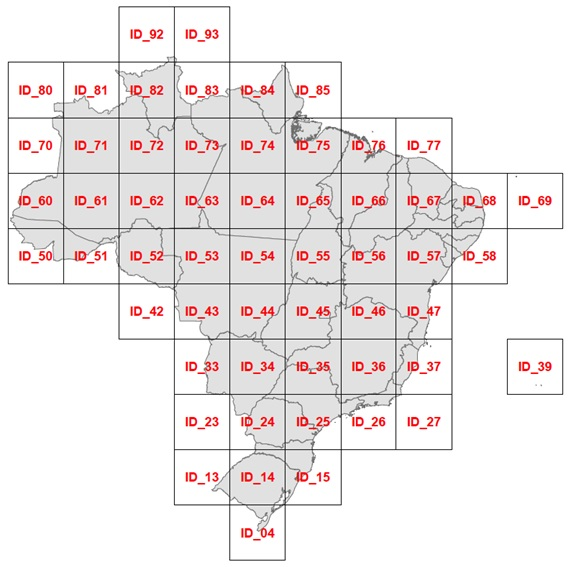
\includegraphics[keepaspectratio]{img/9-grade-estatistica/articulacao.jpg}}

}

\end{figure}%

Esse nível de 500km é também a unidade de distribuição dos arquivos
originais no FTP do IBGE, e cada quadrante recebe um identificador
numérico próprio. O mapa da Figura~\ref{fig-mapa-quadrantes} permite
explorar essa articulação sobre o território nacional, de forma
interativa para quem estiver utilizando o livro no formato digital.
Navegando até Salvador (BA), por exemplo, percebe-se que a cidade é
atravessada pela fronteira entre dois quadrantes, o ID 47, que cobre a
porção Sul, e o ID 57, que cobre a porção Norte. Como veremos na
Seção~\ref{sec-ge-dados}, o quadrante de cada célula acompanha os dados
baixados no campo \texttt{quadrante}, de modo que essa informação hoje
serve para compreender a articulação e localizar os arquivos originais,
e não como uma etapa prévia ao \emph{download}.

\begin{figure}[H]

\caption{\label{fig-mapa-quadrantes}Articulação 500 × 500 km da Grade
Estatística do IBGE sobre os municípios brasileiros. Fontes: IBGE
(2016a); IBGE (2025b).}

\centering{

\pandocbounded{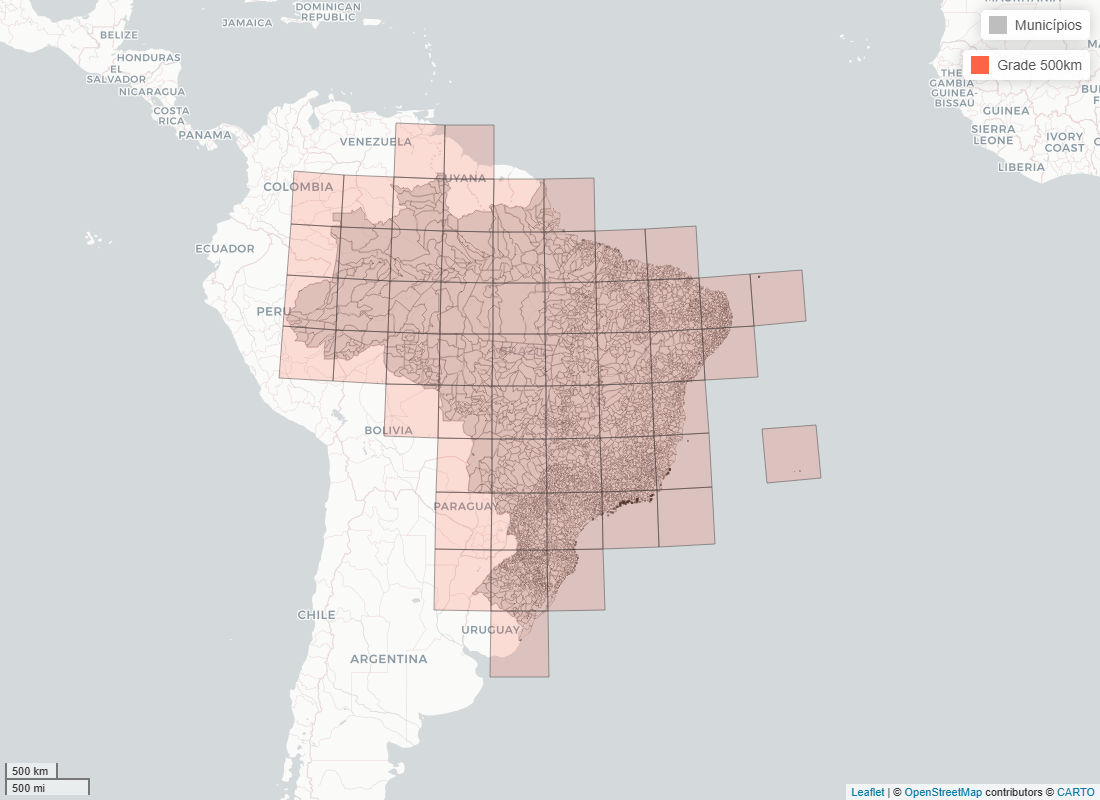
\includegraphics[keepaspectratio]{img/9-grade-estatistica/articulacao_quadrantes.png}}

}

\end{figure}%

As estatísticas das células são derivadas dos microdados \textbf{do
universo} do Censo Demográfico. Lembre-se que o universo compreende a
totalidade dos domicílios visitados pelo recenseador, independentemente
de terem respondido ao questionário básico ou ao da amostra. Esse ponto
é relevante porque os microdados do universo não são disponibilizados ao
público, uma vez que temos acesso apenas aos microdados da amostra,
produto abordado no Capítulo 8. A vinculação entre os microdados do
universo e as células da Grade é feita pelas coordenadas geográficas dos
domicílios registradas no CNEFE.

Os campos estatísticos disponíveis nos arquivos da Grade diferem entre
as duas edições, como mostra a Tabela~\ref{tbl-dicionario-variaveis}. Os
nomes dos campos da edição de 2022 constam no Quadro 4 das notas
metodológicas do IBGE (IBGE, 2025b). O documento metodológico de 2010
(IBGE, 2016a) não apresenta um dicionário de dados equivalente, mas os
nomes e descrição dos campos dessa edição podem ser consultados em
fontes como o OSM Wiki (OpenStreetMap Wiki contributors, 2024). Note que
a versão de 2010 disponibiliza totais de população por sexo
(\texttt{MASC} e \texttt{FEM}), variáveis ausentes na edição de 2022.

A tabela traz uma terceira coluna com os nomes que o pacote
\texttt{geobr} atribui a cada campo, já que é por meio desse pacote que
baixaremos os dados na Seção~\ref{sec-ge-dados}. O \texttt{geobr}
padroniza os nomes em letras minúsculas e harmoniza a população total em
\texttt{pop\_total} nas duas edições, o que elimina boa parte da atenção
que antes era exigida ao comparar os dois Censos. Resta uma divergência
relevante, a dos domicílios, que aparecem como \texttt{dom\_ocu} em 2010
e \texttt{total\_dom} em 2022. Esse é o ponto a vigiar ao realizar
junções entre as bases, e voltaremos a ele na Seção~\ref{sec-ge-maceio}.
O pacote acrescenta ainda quatro campos de identificação territorial que
não existem nos arquivos originais do IBGE.

\begin{longtable}[t]{cccl}

\caption{\label{tbl-dicionario-variaveis}Dicionário de variáveis dos
arquivos da Grade Estatística nas edições de 2010 e 2022, com os nomes
correspondentes no pacote \texttt{geobr}.}

\tabularnewline

\toprule
Campo IBGE (2010) & Campo IBGE (2022) & Campo `geobr` & Descrição\\
\midrule
ID\_UNICO & ID\_UNICO & id\_unico & Identificador único da célula\\
POP & TOTAL & pop\_total & Total de população\\
DOM\_OCU & TOTAL\_DOM & dom\_ocu (2010) / total\_dom (2022) & Total de domicílios ocupados (particular e coletivo)\\
MASC & — & pop\_masc & Total de pessoas do sexo masculino\\
FEM & — & pop\_fem & Total de pessoas do sexo feminino\\
\addlinespace
nome\_1km ... nome\_500km & nome\_1km ... nome\_500KM & nome\_1km ... nome\_500km & Código da célula em cada nível hierárquico\\
QUADRANTE & QUADRANTE & quadrante & Quadrante de articulação (500 x 500 km)\\
— & — & code\_muni & Código do município ao qual a célula foi atribuída\\
— & — & name\_muni & Nome do município\\
— & — & code\_state & Código da unidade da federação\\
\addlinespace
— & — & abbrev\_state & Sigla da unidade da federação\\
\bottomrule

\end{longtable}

É relevante mencionar que o número de células na resolução 200m/1km
também muda entre os Censos. O Censo 2010 gerou 13,3 milhões de células
na resolução básica, sendo 4.610.350 de 200m (34,7\%) e 8.676.139 de 1km
(65,3\%). Em 2022, esse número cresceu para 14,1 milhões, um acréscimo
de cerca de 841 mil células, com 5.486.725 células de 200m (38,84\%) e
8.641.084 células de 1km (61,16\%). Isso ocorre porque, ao se tornarem
urbanizadas\footnote{interceptarem setores censitários do tipo urbano no
  Censo mais recente}, algumas áreas que estavam em células de 1km são
subdivididas em células de 200m. Cabe destacar que células de 200m que
porventura tenham se tornado rurais não passam por um processo de
agregação\footnote{\emph{downgrade}} para a resolução de 1km em um Censo
posterior.

Uma diferença metodológica importante separa as duas edições. No Censo
2010, a geocodificação dos endereços ainda era incompleta, de modo que
parte dos domicílios precisou ser alocada às células por meio de uma
metodologia híbrida que combinava agregação direta com desagregação
proporcional por área. Esse processo introduziu alguma imprecisão na
distribuição espacial da população e gerou uma perda de dados de até 5\%
em algumas áreas. No Censo 2022, a geocodificação foi realizada em seis
níveis de qualidade posicional. Os níveis 5 e 6\footnote{5: mediana das
  coordenadas de endereços em mesmo logradouro, CEP e localidade; 6:
  Coordenadas do centroide do Setor Censitário no qual o endereço está
  contido}, de maior incerteza, foram excluídos da Grade, mas eles
representavam apenas 0,028\% da população total, tornando a perda de
dados praticamente nula (IBGE, 2025b). Detalhes técnicos sobre a
precisão das coordenadas do CNEFE serão melhor explicitados no próximo
capítulo.

A Tabela~\ref{tbl-diferencas-censos} sintetiza as principais diferenças
metodológicas entre os Censos de 2010 e 2022.

\begin{longtable}[t]{lll}

\caption{\label{tbl-diferencas-censos}Principais diferenças
metodológicas na construção da Grade Estatística entre os Censos de 2010
e 2022. Fontes: IBGE (2016a); IBGE (2025b).}

\tabularnewline

\toprule
Aspecto & Censo 2010 & Censo 2022\\
\midrule
Método de alocação & Híbrido (agregação + desagregação proporcional por área) & Agregação direta de endereços geocodificados\\
Geocodificação & Incompleta, complementada por alocação por área & Baseada nos 4 maiores níveis de qualidade; níveis inferiores (5 e 6) excluídos\\
Perda de dados & Até 5\% em algumas regiões & 0,028\% da população\\
Total de células (resolução básica) & 13,3 milhões & 14,1 milhões\\
\bottomrule

\end{longtable}

Com esse panorama metodológico em vista, a próxima seção examina as
principais vantagens e limitações da Grade para fins analíticos.

\section{Vantagens e limitações}\label{sec-ge-vantagens}

A Grade apresenta quatro vantagens analíticas que a distinguem dos
demais produtos do Censo (IBGE, 2016a). A primeira é a
\textbf{estabilidade espaço-temporal}. Como o identificador único de
cada célula é idêntico nas edições de 2010 e 2022, isso contrasta
diretamente com os setores censitários e áreas de ponderação, cujas
fronteiras e identificadores são redesenhados a cada Censo para
acompanhar o crescimento urbano e as necessidades operacionais da
coleta. Salvador, por exemplo, tinha 3.592 setores censitários em 2010 e
4.555 em 2022. Uma comparação direta setor a setor entre as duas edições
seria inviável, pois a maioria dos setores de 2010 não tem
correspondente exato em 2022. Com a Grade, a comparação é feita
simplesmente por meio de uma junção de ambas as tabelas pelo
identificador único, como veremos na Seção~\ref{sec-ge-maceio}.

A segunda vantagem é a \textbf{adaptação a recortes espaciais
personalizados}. As células da Grade funcionam como blocos de construção
que podem ser agregados, de forma aproximada, a qualquer geometria de
interesse, como zonas de tráfego de pesquisas de mobilidade, distritos
sanitários ou bacias hidrográficas. Ao somar as células que intersectam
um recorte de interesse, obtém-se uma estimativa de população para esse
recorte sem necessidade de microdados ou de técnicas de interpolação.

A terceira é a \textbf{hierarquia e flexibilidade}. Os seis níveis de
resolução de quadrículas disponíveis no mesmo sistema de referência
permitem navegar entre escalas de análise com facilidade. Uma análise
que começa na escala metropolitana (nível 50km) pode ser aprofundada
progressivamente até a resolução máxima sem mudar de sistema de
coordenadas ou de conjunto de dados.

A quarta vantagem é a \textbf{versatilidade de representação}. A
estrutura retangular regular da Grade permite tratar os dados tanto como
vetor quanto como \emph{raster}. Essa dualidade amplia o conjunto de
ferramentas analíticas disponíveis, abrindo a possibilidade de aplicar
métodos de processamento de imagem e análise espacial matricial.

Todavia, há restrições importantes com relação ao uso da Grade. A
principal delas é o \textbf{reduzido número de variáveis} disponíveis.
Com apenas população total e domicílios ocupados, ela não permite
análises de renda, escolaridade, raça, acesso a serviços ou qualquer
outro atributo socioeconômico. Para essas análises, os Microdados e os
Agregados continuam sendo indispensáveis.

Uma segunda limitação diz respeito à geometria retangular das células.
Como discutido no Capítulo 7 ao apresentar as grades hexagonais H3,
células quadradas possuem dois tipos de vizinhança, os que compartilham
aresta e os que compartilham apenas um vértice, com distância entre
centros cerca de 41\% maior neste último caso. Essa \textbf{assimetria}
implica que análises de proximidade e acessibilidade, nas quais a
equidistância entre vizinhos é uma propriedade desejável, produzem
resultados geometricamente menos precisos em grades retangulares do que
em grades hexagonais. Acrescenta-se ainda que anéis concêntricos de
hexágonos aproximam círculos com mais fidelidade do que anéis quadrados,
tornando a delimitação de zonas de influência e buffer mais natural
naquele formato.

Por fim, a \textbf{forma de distribuição} dos dados pelo IBGE cria uma
etapa adicional de trabalho antes do \emph{download}. A Grade
Estatística na sua melhor resolução (200m/1km) não é disponibilizada
como um arquivo único para o país ou por município, mas em recortes por
quadrantes de 500 x 500 km. Antes de baixar os dados, é preciso
identificar quais quadrantes cobrem o município de interesse.
Felizmente, essa restrição foi contornada mais recentemente com
melhorias implementadas no pacote \texttt{geobr} do IPEA, que permite
obter esses dados por município ou UF.

Com essas vantagens e limitações em mente, a próxima seção mostra como
obter a Grade no R e transformá-la em mapas.

\section{Obtendo e mapeando os dados no R}\label{sec-ge-dados}

\subsection{Obtenção da grade por
município}\label{obtenuxe7uxe3o-da-grade-por-municuxedpio}

O pacote \texttt{geobr}, a partir da sua versão 2.0.0, passou a
disponibilizar a grade estatística recortada por município de interesse
na função \texttt{read\_statistical\_grid()}. São necessários apenas
dois argumentos, o ano da edição do Censo em \texttt{year} e o código de
7 dígitos do IBGE em \texttt{code\_muni}. O código a seguir obtém as
duas edições da Grade para Salvador (BA), cujo código municipal é
2927408.

\begin{Shaded}
\begin{Highlighting}[]
\FunctionTok{library}\NormalTok{(tidyverse)}
\FunctionTok{library}\NormalTok{(sf)}
\FunctionTok{library}\NormalTok{(geobr)}
\end{Highlighting}
\end{Shaded}

\begin{verbatim}
Warning: pacote 'geobr' foi compilado no R versão 4.6.1
\end{verbatim}

\begin{Shaded}
\begin{Highlighting}[]
\NormalTok{ge\_ssa2010 }\OtherTok{\textless{}{-}} \FunctionTok{read\_statistical\_grid}\NormalTok{(}\AttributeTok{year =} \DecValTok{2010}\NormalTok{, }\AttributeTok{code\_muni =} \DecValTok{2927408}\NormalTok{)}
\NormalTok{ge\_ssa2022 }\OtherTok{\textless{}{-}} \FunctionTok{read\_statistical\_grid}\NormalTok{(}\AttributeTok{year =} \DecValTok{2022}\NormalTok{, }\AttributeTok{code\_muni =} \DecValTok{2927408}\NormalTok{)}
\end{Highlighting}
\end{Shaded}

Duas linhas de código substituem todo o trabalho de identificar
quadrantes, baixar arquivos compactados, empilhá-los e recortá-los aos
limites municipais. A função também mantém, por padrão, um cache local
dos arquivos baixados (\texttt{cache\ =\ TRUE}), de modo que uma segunda
chamada dentro da mesma sessão do R não repete o \emph{download}.

\begin{tcolorbox}[enhanced jigsaw, arc=.35mm, bottomrule=.15mm, bottomtitle=1mm, breakable, colback=white, colbacktitle=quarto-callout-tip-color!10!white, colframe=quarto-callout-tip-color-frame, coltitle=black, left=2mm, leftrule=.75mm, opacityback=0, opacitybacktitle=0.6, rightrule=.15mm, title=\textcolor{quarto-callout-tip-color}{\faLightbulb}\hspace{0.5em}{Outros recortes espaciais}, titlerule=0mm, toprule=.15mm, toptitle=1mm]

O argumento \texttt{code\_muni} aceita mais do que o código de um
município. Passando a sigla ou o código de dois dígitos de uma unidade
da federação, a função baixa a Grade de todo o estado, como em
\texttt{read\_statistical\_grid(year\ =\ 2022,\ code\_muni\ =\ "BA")} ou
\texttt{code\_muni\ =\ 29}. Com \texttt{code\_muni\ =\ "all"}, obtém-se
a Grade do país inteiro. Para consultar códigos municipais sem sair do
R, use \texttt{geobr::lookup\_muni()}.

\end{tcolorbox}

\begin{tcolorbox}[enhanced jigsaw, arc=.35mm, bottomrule=.15mm, bottomtitle=1mm, breakable, colback=white, colbacktitle=quarto-callout-note-color!10!white, colframe=quarto-callout-note-color-frame, coltitle=black, left=2mm, leftrule=.75mm, opacityback=0, opacitybacktitle=0.6, rightrule=.15mm, title=\textcolor{quarto-callout-note-color}{\faInfo}\hspace{0.5em}{Grades muito grandes e os arquivos originais}, titlerule=0mm, toprule=.15mm, toptitle=1mm]

A Grade de um município cabe confortavelmente na memória, mas o mesmo
não vale para um estado populoso ou para o país, que reúne mais de 14
milhões de células. Para esses casos, o argumento \texttt{output} aceita
os valores \texttt{"duckdb"} e \texttt{"arrow"}, que devolvem uma tabela
espacial preguiçosa em vez de um objeto \texttt{sf} carregado na
memória. Assim, é possível filtrar e agregar os dados antes de trazê-los
para a sessão do R.

Os arquivos originais do IBGE, organizados por quadrante de 500 x 500 km
e em formato \emph{shapefile}, continuam disponíveis no servidor FTP do
instituto, em
\url{https://geoftp.ibge.gov.br/recortes_para_fins_estatisticos/grade_estatistica/}.

\end{tcolorbox}

\subsection{Mapeando os resultados}\label{mapeando-os-resultados}

Vamos primeiramente observar o formato destes arquivos de grade,
relativo aos Censos de 2010 (Figura~\ref{fig-grade-ssa-2010}) e de 2022
(Figura~\ref{fig-grade-ssa-2022}), em que cada polígono corresponde a
uma célula de 200m ou 1km, utilizando o \texttt{ggplot2}. Note como, em
2022, as poucas quadrículas do tipo rural de 2010 foram subdivididas em
quadrículas do tipo urbano, de 200m\footnote{Curiosidade: essa
  urbanização ocorreu na Ilha dos Frades, que pertence ao município de
  Salvador}.

\begin{Shaded}
\begin{Highlighting}[]
\NormalTok{ge\_ssa2010 }\SpecialCharTok{|\textgreater{}}
  \FunctionTok{ggplot}\NormalTok{() }\SpecialCharTok{+}
  \FunctionTok{geom\_sf}\NormalTok{() }\SpecialCharTok{+}
  \FunctionTok{theme\_minimal}\NormalTok{()}
\end{Highlighting}
\end{Shaded}

\begin{figure}[H]

\caption{\label{fig-grade-ssa-2010}Resolução das células da Grade
Estatística de 2010 em Salvador (BA).}

\centering{

\pandocbounded{
\includegraphics[keepaspectratio]{9-grade-estatistica_files/figure-pdf/fig-grade-ssa-2010-1.pdf}}

}

\end{figure}%

\begin{Shaded}
\begin{Highlighting}[]
\NormalTok{ge\_ssa2022 }\SpecialCharTok{|\textgreater{}}
  \FunctionTok{ggplot}\NormalTok{() }\SpecialCharTok{+}
  \FunctionTok{geom\_sf}\NormalTok{() }\SpecialCharTok{+}
  \FunctionTok{theme\_minimal}\NormalTok{()}
\end{Highlighting}
\end{Shaded}

\begin{figure}[H]

\caption{\label{fig-grade-ssa-2022}Resolução das células da Grade
Estatística de 2022 em Salvador (BA). Nota: observe que não há mais as
quadrículas do tipo rural (resolução de 1km)}

\centering{

\pandocbounded{
\includegraphics[keepaspectratio]{9-grade-estatistica_files/figure-pdf/fig-grade-ssa-2022-1.pdf}}

}

\end{figure}%

É igualmente interessante explorar as tabelas de dados que esses
arquivos geográficos carregam consigo. Como cada objeto traz mais de uma
dezena de colunas, vamos selecionar apenas os campos que nos interessam
antes de visualizar os primeiros registros.

\begin{Shaded}
\begin{Highlighting}[]
\NormalTok{ge\_ssa2010 }\SpecialCharTok{|\textgreater{}}
  \FunctionTok{st\_drop\_geometry}\NormalTok{() }\SpecialCharTok{|\textgreater{}}
  \FunctionTok{select}\NormalTok{(id\_unico, pop\_total, dom\_ocu, quadrante) }\SpecialCharTok{|\textgreater{}}
  \FunctionTok{head}\NormalTok{()}
\end{Highlighting}
\end{Shaded}

\begin{verbatim}
# A tibble: 6 x 4
  id_unico         pop_total dom_ocu quadrante
  <chr>                <int>   <int> <chr>    
1 200ME66358N98634         0       0 ID_57    
2 200ME66358N98636         0       0 ID_57    
3 200ME66356N98638         0       0 ID_57    
4 200ME66358N98638         0       0 ID_57    
5 200ME66356N98640         0       0 ID_57    
6 200ME66358N98640         0       0 ID_57    
\end{verbatim}

\begin{Shaded}
\begin{Highlighting}[]
\NormalTok{ge\_ssa2022 }\SpecialCharTok{|\textgreater{}}
  \FunctionTok{st\_drop\_geometry}\NormalTok{() }\SpecialCharTok{|\textgreater{}}
  \FunctionTok{select}\NormalTok{(id\_unico, pop\_total, total\_dom, quadrante) }\SpecialCharTok{|\textgreater{}}
  \FunctionTok{head}\NormalTok{()}
\end{Highlighting}
\end{Shaded}

\begin{verbatim}
# A tibble: 6 x 4
  id_unico         pop_total total_dom quadrante
  <chr>                <dbl>     <dbl> <chr>    
1 200ME66358N98634         0         0 ID_57    
2 200ME66358N98636         0         0 ID_57    
3 200ME66356N98638         0         0 ID_57    
4 200ME66358N98638         0         0 ID_57    
5 200ME66356N98640         0         0 ID_57    
6 200ME66358N98640         0         0 ID_57    
\end{verbatim}

Duas coisas chamam a atenção nessas tabelas. A primeira é que o campo
\texttt{id\_unico} de cada célula permite identificar sua resolução.
Aqueles que começam com \texttt{"200M"} correspondem a células de 200m
(áreas urbanas), enquanto os que começam com \texttt{"1KM"} correspondem
a células de 1km (áreas rurais). A segunda é o campo \texttt{quadrante},
que registra o quadrante de 500 x 500 km ao qual a célula pertence.
Listando seus valores distintos, confirmamos o que o mapa da
Figura~\ref{fig-mapa-quadrantes} mostrava, já que Salvador se distribui
entre dois quadrantes.

\begin{Shaded}
\begin{Highlighting}[]
\FunctionTok{unique}\NormalTok{(ge\_ssa2022}\SpecialCharTok{$}\NormalTok{quadrante)}
\end{Highlighting}
\end{Shaded}

\begin{verbatim}
[1] "ID_57" "ID_47"
\end{verbatim}

Entendida essa estrutura, podemos produzir alguns mapas coropléticos.
Para o mapa de 2010 (Figura~\ref{fig-grade-ssa-pop2010}), observe que
passamos a variável \texttt{pop\_total} no mapeamento estético da cor de
preenchimento dos polígonos (\texttt{fill}) e editamos essa coloração
para a paleta ``Reds'' em \texttt{scale\_fill\_distiller()}. Neste caso,
quanto mais intenso na cor vermelha, maior a população naquela
quadrícula. O mapa de 2022 (Figura~\ref{fig-grade-ssa-pop2022}) usa
exatamente o mesmo código, trocando apenas o objeto de entrada. Essa
repetição é possível porque o \texttt{geobr} padroniza o nome da
população total como \texttt{pop\_total} nas duas edições, poupando o
trabalho de lidar com os nomes originais \texttt{POP} e \texttt{TOTAL}
dos arquivos do IBGE.

\begin{Shaded}
\begin{Highlighting}[]
\FunctionTok{ggplot}\NormalTok{(ge\_ssa2010) }\SpecialCharTok{+}
  \FunctionTok{geom\_sf}\NormalTok{(}\FunctionTok{aes}\NormalTok{(}\AttributeTok{fill =}\NormalTok{ pop\_total), }\AttributeTok{color =} \ConstantTok{NA}\NormalTok{) }\SpecialCharTok{+}
  \FunctionTok{scale\_fill\_distiller}\NormalTok{(}
    \AttributeTok{palette =} \StringTok{"Reds"}\NormalTok{,}
    \AttributeTok{direction =} \DecValTok{1}\NormalTok{,}
    \AttributeTok{name =} \StringTok{"Pop. total"}\NormalTok{,}
    \AttributeTok{na.value =} \StringTok{"gray90"}\NormalTok{,}
    \AttributeTok{labels =}\NormalTok{ scales}\SpecialCharTok{::}\FunctionTok{label\_number}\NormalTok{(}\AttributeTok{big.mark =} \StringTok{"."}\NormalTok{, }\AttributeTok{decimal.mark =} \StringTok{","}\NormalTok{)}
\NormalTok{  ) }\SpecialCharTok{+}
  \FunctionTok{coord\_sf}\NormalTok{(}\AttributeTok{expand =} \ConstantTok{FALSE}\NormalTok{) }\SpecialCharTok{+}
  \FunctionTok{theme\_minimal}\NormalTok{() }\SpecialCharTok{+}
  \FunctionTok{theme}\NormalTok{(}
    \AttributeTok{axis.text  =} \FunctionTok{element\_blank}\NormalTok{(),}
    \AttributeTok{axis.ticks =} \FunctionTok{element\_blank}\NormalTok{(),}
    \AttributeTok{panel.grid =} \FunctionTok{element\_blank}\NormalTok{()}
\NormalTok{  )}
\end{Highlighting}
\end{Shaded}

\begin{figure}[H]

\caption{\label{fig-grade-ssa-pop2010}Distribuição da população total
por célula da Grade Estatística de 2010 em Salvador (BA).}

\centering{

\pandocbounded{
\includegraphics[keepaspectratio]{9-grade-estatistica_files/figure-pdf/fig-grade-ssa-pop2010-1.pdf}}

}

\end{figure}%

\begin{Shaded}
\begin{Highlighting}[]
\FunctionTok{ggplot}\NormalTok{(ge\_ssa2022) }\SpecialCharTok{+}
  \FunctionTok{geom\_sf}\NormalTok{(}\FunctionTok{aes}\NormalTok{(}\AttributeTok{fill =}\NormalTok{ pop\_total), }\AttributeTok{color =} \ConstantTok{NA}\NormalTok{) }\SpecialCharTok{+}
  \FunctionTok{scale\_fill\_distiller}\NormalTok{(}
    \AttributeTok{palette =} \StringTok{"Reds"}\NormalTok{,}
    \AttributeTok{direction =} \DecValTok{1}\NormalTok{,}
    \AttributeTok{name =} \StringTok{"Pop. total"}\NormalTok{,}
    \AttributeTok{na.value =} \StringTok{"gray90"}\NormalTok{,}
    \AttributeTok{labels =}\NormalTok{ scales}\SpecialCharTok{::}\FunctionTok{label\_number}\NormalTok{(}\AttributeTok{big.mark =} \StringTok{"."}\NormalTok{, }\AttributeTok{decimal.mark =} \StringTok{","}\NormalTok{)}
\NormalTok{  ) }\SpecialCharTok{+}
  \FunctionTok{coord\_sf}\NormalTok{(}\AttributeTok{expand =} \ConstantTok{FALSE}\NormalTok{) }\SpecialCharTok{+}
  \FunctionTok{theme\_minimal}\NormalTok{() }\SpecialCharTok{+}
  \FunctionTok{theme}\NormalTok{(}
    \AttributeTok{axis.text  =} \FunctionTok{element\_blank}\NormalTok{(),}
    \AttributeTok{axis.ticks =} \FunctionTok{element\_blank}\NormalTok{(),}
    \AttributeTok{panel.grid =} \FunctionTok{element\_blank}\NormalTok{()}
\NormalTok{  )}
\end{Highlighting}
\end{Shaded}

\begin{figure}[H]

\caption{\label{fig-grade-ssa-pop2022}Distribuição da população total
por célula da Grade Estatística de 2022 em Salvador (BA).}

\centering{

\pandocbounded{
\includegraphics[keepaspectratio]{9-grade-estatistica_files/figure-pdf/fig-grade-ssa-pop2022-1.pdf}}

}

\end{figure}%

Os dois mapas de população revelam a distribuição espacial de Salvador
com uma granularidade muito superior à dos setores censitários. Porém, a
comparação visual entre eles para verificar onde houve crescimento ou
retração entre as duas edições é mais difícil. A próxima seção explora
esse potencial comparativo de forma sistemática, usando Maceió como caso
de análise. Essa escolha revela o poder da Grade Estatística de mapear
fenômenos importantes como deslocamentos populacionais significativos
causados por desastres ambientais.

\section{Variação populacional entre Censos: o caso de
Maceió}\label{sec-ge-maceio}

A estabilidade do identificador \texttt{id\_unico} entre as edições do
Censo é a vantagem mais distintiva da Grade Estatística. Ela permite
comparar diretamente a população e os domicílios de cada célula entre
2010 e 2022, identificando onde houve crescimento, estagnação ou
declínio com uma resolução espacial de 200 metros. Para ilustrar essa
capacidade, analisaremos o caso de Maceió (AL), onde esse tipo de
comparação revela um fenômeno de grande impacto social e urbano.

Entre os dois Censos, a capital alagoana viveu os afundamentos do solo
causados pela mineração de sal-gema, especialmente nos bairros de
Pinheiro, Mutange, Bebedouro e Bom Parto. A subsidência progressiva do
terreno, decorrente da dissolução das cavernas subterrâneas de onde o
sal era extraído, tornou inabitáveis vastas áreas residenciais nesses
bairros. A partir de 2018, o processo de evacuação compulsória de
moradores se intensificou, resultando no deslocamento de dezenas de
milhares de pessoas até o período do Censo 2022. O impacto desse
fenômeno na distribuição espacial da população é precisamente o tipo de
mudança que a comparação entre grades censitárias é capaz de revelar.

O procedimento de obtenção dos dados é o mesmo que usamos para Salvador,
bastando trocar o código municipal para 2704302. Diferentemente de
Salvador, Maceió está integralmente contida em um único quadrante, o ID
58, o que pode ser conferido inspecionando o campo \texttt{quadrante}
depois do \emph{download}.

\begin{Shaded}
\begin{Highlighting}[]
\FunctionTok{library}\NormalTok{(tidyverse)}
\FunctionTok{library}\NormalTok{(sf)}
\FunctionTok{library}\NormalTok{(geobr)}

\NormalTok{ge\_mcz2010 }\OtherTok{\textless{}{-}} \FunctionTok{read\_statistical\_grid}\NormalTok{(}\AttributeTok{year =} \DecValTok{2010}\NormalTok{, }\AttributeTok{code\_muni =} \DecValTok{2704302}\NormalTok{)}
\NormalTok{ge\_mcz2022 }\OtherTok{\textless{}{-}} \FunctionTok{read\_statistical\_grid}\NormalTok{(}\AttributeTok{year =} \DecValTok{2022}\NormalTok{, }\AttributeTok{code\_muni =} \DecValTok{2704302}\NormalTok{)}

\FunctionTok{unique}\NormalTok{(ge\_mcz2022}\SpecialCharTok{$}\NormalTok{quadrante)}
\end{Highlighting}
\end{Shaded}

\begin{verbatim}
[1] "ID_58"
\end{verbatim}

Com os dados, é possível observar a grade de Maceió em ambos os anos em
Figura~\ref{fig-grade-mcz-2010} e Figura~\ref{fig-grade-mcz-2022}:

\begin{Shaded}
\begin{Highlighting}[]
\NormalTok{ge\_mcz2010 }\SpecialCharTok{|\textgreater{}}
  \FunctionTok{ggplot}\NormalTok{() }\SpecialCharTok{+}
  \FunctionTok{geom\_sf}\NormalTok{() }\SpecialCharTok{+}
  \FunctionTok{theme\_minimal}\NormalTok{()}
\end{Highlighting}
\end{Shaded}

\begin{figure}[H]

\caption{\label{fig-grade-mcz-2010}Resolução das células da Grade
Estatística de 2010 em Maceió (AL).}

\centering{

\pandocbounded{
\includegraphics[keepaspectratio]{9-grade-estatistica_files/figure-pdf/fig-grade-mcz-2010-1.pdf}}

}

\end{figure}%

\begin{Shaded}
\begin{Highlighting}[]
\NormalTok{ge\_mcz2022 }\SpecialCharTok{|\textgreater{}}
  \FunctionTok{ggplot}\NormalTok{() }\SpecialCharTok{+}
  \FunctionTok{geom\_sf}\NormalTok{() }\SpecialCharTok{+}
  \FunctionTok{theme\_minimal}\NormalTok{()}
\end{Highlighting}
\end{Shaded}

\begin{figure}[H]

\caption{\label{fig-grade-mcz-2022}Resolução das células da Grade
Estatística de 2022 em Maceió (AL).}

\centering{

\pandocbounded{
\includegraphics[keepaspectratio]{9-grade-estatistica_files/figure-pdf/fig-grade-mcz-2022-1.pdf}}

}

\end{figure}%

\subsection{Verificando a correspondência entre as
edições}\label{sec-ge-correspondencia}

Com os objetos \texttt{ge\_mcz2010} e \texttt{ge\_mcz2022} carregados, é
tentador partir direto para um \emph{join} por \texttt{id\_unico}. Antes
disso, porém, convém verificar se a correspondência entre as duas
edições é de fato completa. A estabilidade do identificador garante que
uma célula com o mesmo \texttt{id\_unico} representa o mesmo pedaço de
território nos dois anos, mas não garante que toda célula de 2022 tenha
uma correspondente em 2010.

Há dois motivos para isso. O primeiro é a subdivisão discutida na
Seção~\ref{sec-aspectos_metodologicos}, em que uma célula de 1 km de
2010 se torna um conjunto de células de 200 m em 2022 ao ser
classificada como urbana. Nesse caso a correspondência existe, mas é de
\textbf{hierarquia diferente}, e a chave que a revela é o campo
\texttt{nome\_1km}, que registra a célula de 1 km à qual cada célula de
200 m pertence. O segundo motivo é a ausência pura e simples de
correspondente, seja porque a célula não existia na edição anterior,
seja pelas razões de atribuição territorial descritas na nota
metodológica ao final desta seção.

Vamos então classificar cada célula de 2022 em três situações, tomando a
edição mais recente como ponto de partida. Uma célula tem
correspondência \textbf{direta} se o seu \texttt{id\_unico} aparece em
2010. Se não aparece, mas é uma célula de 200 m cujo \texttt{nome\_1km}
consta como célula de 1 km em 2010, então ela é fruto de
\textbf{subdivisão}. Restando as duas hipóteses, a célula fica
\textbf{sem correspondência}.

\begin{Shaded}
\begin{Highlighting}[]
\NormalTok{ids\_2010     }\OtherTok{\textless{}{-}}\NormalTok{ ge\_mcz2010}\SpecialCharTok{$}\NormalTok{id\_unico}
\NormalTok{ids\_1km\_2010 }\OtherTok{\textless{}{-}}\NormalTok{ ids\_2010[}\FunctionTok{str\_starts}\NormalTok{(ids\_2010, }\StringTok{"1KM"}\NormalTok{)]}

\NormalTok{niveis }\OtherTok{\textless{}{-}} \FunctionTok{c}\NormalTok{(}\StringTok{"direta"}\NormalTok{, }\StringTok{"subdividida"}\NormalTok{, }\StringTok{"sem correspondência"}\NormalTok{)}

\NormalTok{corresp\_2022 }\OtherTok{\textless{}{-}}\NormalTok{ ge\_mcz2022 }\SpecialCharTok{|\textgreater{}}
  \FunctionTok{st\_drop\_geometry}\NormalTok{() }\SpecialCharTok{|\textgreater{}}
  \FunctionTok{mutate}\NormalTok{(}
    \AttributeTok{situacao =} \FunctionTok{case\_when}\NormalTok{(}
\NormalTok{      id\_unico }\SpecialCharTok{\%in\%}\NormalTok{ ids\_2010                                     }\SpecialCharTok{\textasciitilde{}} \StringTok{"direta"}\NormalTok{,}
      \FunctionTok{str\_starts}\NormalTok{(id\_unico, }\StringTok{"200M"}\NormalTok{) }\SpecialCharTok{\&}\NormalTok{ nome\_1km }\SpecialCharTok{\%in\%}\NormalTok{ ids\_1km\_2010  }\SpecialCharTok{\textasciitilde{}} \StringTok{"subdividida"}\NormalTok{,}
      \AttributeTok{.default                                                   =} \StringTok{"sem correspondência"}
\NormalTok{    ),}
    \AttributeTok{situacao =} \FunctionTok{factor}\NormalTok{(situacao, }\AttributeTok{levels =}\NormalTok{ niveis)}
\NormalTok{  )}

\NormalTok{corresp\_2022 }\SpecialCharTok{|\textgreater{}}
  \FunctionTok{group\_by}\NormalTok{(situacao, }\AttributeTok{.drop =} \ConstantTok{FALSE}\NormalTok{) }\SpecialCharTok{|\textgreater{}}
  \FunctionTok{summarize}\NormalTok{(}\AttributeTok{celulas =} \FunctionTok{n}\NormalTok{(), }\AttributeTok{pop =} \FunctionTok{sum}\NormalTok{(pop\_total), }\AttributeTok{.groups =} \StringTok{"drop"}\NormalTok{)}
\end{Highlighting}
\end{Shaded}

\begin{verbatim}
# A tibble: 3 x 3
  situacao            celulas    pop
  <fct>                 <int>  <dbl>
1 direta                 6294 956251
2 subdividida               0      0
3 sem correspondência      49    559
\end{verbatim}

O teste mostra que, em Maceió, \textbf{nenhuma} célula resultou de
subdivisão. A quase totalidade tem correspondência direta, e sobra um
resíduo de algumas dezenas de células sem par, que reúnem pouco mais de
meia centena de habitantes. Convém repetir a verificação no sentido
inverso, partindo de 2010, para detectar células que existiam naquela
edição e não têm correspondente em 2022.

\begin{Shaded}
\begin{Highlighting}[]
\NormalTok{filhas\_2022 }\OtherTok{\textless{}{-}}\NormalTok{ ge\_mcz2022 }\SpecialCharTok{|\textgreater{}}
  \FunctionTok{st\_drop\_geometry}\NormalTok{() }\SpecialCharTok{|\textgreater{}}
  \FunctionTok{filter}\NormalTok{(}\FunctionTok{str\_starts}\NormalTok{(id\_unico, }\StringTok{"200M"}\NormalTok{)) }\SpecialCharTok{|\textgreater{}}
  \FunctionTok{pull}\NormalTok{(nome\_1km)}

\NormalTok{corresp\_2010 }\OtherTok{\textless{}{-}}\NormalTok{ ge\_mcz2010 }\SpecialCharTok{|\textgreater{}}
  \FunctionTok{st\_drop\_geometry}\NormalTok{() }\SpecialCharTok{|\textgreater{}}
  \FunctionTok{mutate}\NormalTok{(}
    \AttributeTok{situacao =} \FunctionTok{case\_when}\NormalTok{(}
\NormalTok{      id\_unico }\SpecialCharTok{\%in\%}\NormalTok{ ge\_mcz2022}\SpecialCharTok{$}\NormalTok{id\_unico }\SpecialCharTok{\textasciitilde{}} \StringTok{"direta"}\NormalTok{,}
\NormalTok{      id\_unico }\SpecialCharTok{\%in\%}\NormalTok{ filhas\_2022         }\SpecialCharTok{\textasciitilde{}} \StringTok{"subdividida"}\NormalTok{,}
      \AttributeTok{.default                          =} \StringTok{"sem correspondência"}
\NormalTok{    ),}
    \AttributeTok{situacao =} \FunctionTok{factor}\NormalTok{(situacao, }\AttributeTok{levels =}\NormalTok{ niveis)}
\NormalTok{  )}

\NormalTok{corresp\_2010 }\SpecialCharTok{|\textgreater{}}
  \FunctionTok{group\_by}\NormalTok{(situacao, }\AttributeTok{.drop =} \ConstantTok{FALSE}\NormalTok{) }\SpecialCharTok{|\textgreater{}}
  \FunctionTok{summarize}\NormalTok{(}\AttributeTok{celulas =} \FunctionTok{n}\NormalTok{(), }\AttributeTok{pop =} \FunctionTok{sum}\NormalTok{(pop\_total), }\AttributeTok{.groups =} \StringTok{"drop"}\NormalTok{)}
\end{Highlighting}
\end{Shaded}

\begin{verbatim}
# A tibble: 3 x 3
  situacao            celulas    pop
  <fct>                 <int>  <int>
1 direta                 6294 920809
2 subdividida               0      0
3 sem correspondência      24   1225
\end{verbatim}

O resultado confirma o diagnóstico. Não há subdivisões em nenhum dos
dois sentidos e o mesmo conjunto de células se corresponde diretamente
nas duas edições, cobrindo mais de 99\% da população municipal em cada
ano. Para Maceió, portanto, o \emph{join} direto por \texttt{id\_unico}
é legítimo, e a etapa de agregação hierárquica que seria necessária em
outros municípios pode ser dispensada.

Vale insistir que essa conclusão é um resultado do teste empírico que
estamos realizando. Em municípios que se urbanizaram intensamente no
período, a categoria ``subdividida'' é volumosa e ignorá-la produziria
buracos nos mapas de variação. O callout ao final da seção detalha esse
ponto.

Feita a verificação, o \emph{join} é simples. Renomeamos as variáveis
com sufixos de ano dentro do próprio \texttt{select()}, o que resolve
duas coisas de uma vez. A primeira é a colisão de nomes, já que a
população total se chama \texttt{pop\_total} nas duas edições e o
\emph{join} produziria colunas ambíguas do tipo \texttt{pop\_total.x} e
\texttt{pop\_total.y}. A segunda é a divergência entre \texttt{dom\_ocu}
e \texttt{total\_dom}, apontada na
Tabela~\ref{tbl-dicionario-variaveis}.

\begin{Shaded}
\begin{Highlighting}[]
\NormalTok{mcz\_ge }\OtherTok{\textless{}{-}}\NormalTok{ ge\_mcz2010 }\SpecialCharTok{|\textgreater{}}
  \FunctionTok{select}\NormalTok{(id\_unico, }\AttributeTok{pop\_2010 =}\NormalTok{ pop\_total, }\AttributeTok{dom\_2010 =}\NormalTok{ dom\_ocu) }\SpecialCharTok{|\textgreater{}}
  \FunctionTok{left\_join}\NormalTok{(}
\NormalTok{    ge\_mcz2022 }\SpecialCharTok{|\textgreater{}}
      \FunctionTok{st\_drop\_geometry}\NormalTok{() }\SpecialCharTok{|\textgreater{}}
      \FunctionTok{select}\NormalTok{(id\_unico, }\AttributeTok{pop\_2022 =}\NormalTok{ pop\_total, }\AttributeTok{dom\_2022 =}\NormalTok{ total\_dom),}
    \AttributeTok{by =} \FunctionTok{join\_by}\NormalTok{(id\_unico)}
\NormalTok{  ) }\SpecialCharTok{|\textgreater{}}
  \FunctionTok{mutate}\NormalTok{(}
    \AttributeTok{varpop =}\NormalTok{ pop\_2022 }\SpecialCharTok{{-}}\NormalTok{ pop\_2010,}
    \AttributeTok{vardom =}\NormalTok{ dom\_2022 }\SpecialCharTok{{-}}\NormalTok{ dom\_2010}
\NormalTok{  )}
\end{Highlighting}
\end{Shaded}

\begin{tcolorbox}[enhanced jigsaw, arc=.35mm, bottomrule=.15mm, bottomtitle=1mm, breakable, colback=white, colbacktitle=quarto-callout-note-color!10!white, colframe=quarto-callout-note-color-frame, coltitle=black, left=2mm, leftrule=.75mm, opacityback=0, opacitybacktitle=0.6, rightrule=.15mm, title=\textcolor{quarto-callout-note-color}{\faInfo}\hspace{0.5em}{Três cuidados ao comparar edições da Grade}, titlerule=0mm, toprule=.15mm, toptitle=1mm]

\textbf{1. A subdivisão existe, ainda que não em Maceió.} Aplicando o
mesmo teste a todo o estado de Alagoas, encontram-se 463 células de 1 km
de 2010 que foram substituídas por células de 200 m em 2022, das quais
372 tinham população, somando cerca de 110 mil habitantes. Elas se
concentram em municípios que se urbanizaram no período, com destaque
para Arapiraca. Nesses casos, é preciso agregar as células de 2022 de
volta ao nível de 1 km antes do \emph{join}, agrupando por
\texttt{nome\_1km} e somando população e domicílios.

\textbf{2. Testar a resolução pelo prefixo do identificador não basta.}
Uma tentação natural é comparar apenas os conjuntos de células de 1 km
das duas edições e supor que as que desapareceram foram subdivididas.
Esse atalho mistura fenômenos distintos, porque uma célula pode sumir do
conjunto sem ter sido subdividida. A verificação confiável é a que
fizemos aqui, que procura as células filhas de 200 m pelo campo
\texttt{nome\_1km}.

\textbf{3. O \texttt{geobr} descarta células sem município.} Ao preparar
os dados, o pacote calcula o centroide de cada célula e o cruza com a
malha municipal do ano correspondente. Células cujo centroide cai fora
de qualquer polígono municipal, tipicamente sobre lagoas, baías e o mar,
ficam sem \texttt{code\_muni} e não são devolvidas por nenhuma consulta
a município ou estado. No quadrante que cobre Alagoas, isso alcança
12.442 das 145.199 células de 2010. Na área de Maceió são 143 células,
quase todas de população zero por estarem sobre a Lagoa Mundaú, embora
nove delas somem 226 habitantes. Essa é a razão pela qual a contagem de
células obtida pelo \texttt{geobr} é menor do que a dos arquivos
originais do FTP, e ajuda a explicar o resíduo sem correspondência dos
testes acima.

\end{tcolorbox}

As células sem correspondência não encontram par no \emph{join} e
recebem \texttt{NA} nas variações, sendo desenhadas em cinza pelo
argumento \texttt{na.value\ =\ "gray90"} dos mapas a seguir.

Com \texttt{mcz\_ge} pronto, podemos visualizar as variações de
população e domicílios ocupados nos mapas interativos da
Figura~\ref{fig-mcz-varpop} e Figura~\ref{fig-mcz-vardom}. Para que a
escala de cores destaque tanto as perdas quanto os ganhos de forma
simétrica, usamos a paleta divergente \texttt{"RdBu"} com limites iguais
em valor absoluto nos dois extremos, calculados a partir de
\texttt{max(abs(...))}. Assim, o branco central da paleta corresponde
sempre ao zero, vermelho indica redução e azul indica aumento.

\begin{Shaded}
\begin{Highlighting}[]
\NormalTok{lim\_pop }\OtherTok{\textless{}{-}} \FunctionTok{max}\NormalTok{(}\FunctionTok{abs}\NormalTok{(mcz\_ge}\SpecialCharTok{$}\NormalTok{varpop), }\AttributeTok{na.rm =} \ConstantTok{TRUE}\NormalTok{)}

\FunctionTok{ggplot}\NormalTok{(mcz\_ge) }\SpecialCharTok{+}
  \FunctionTok{geom\_sf}\NormalTok{(}\FunctionTok{aes}\NormalTok{(}\AttributeTok{fill =}\NormalTok{ varpop), }\AttributeTok{color =} \ConstantTok{NA}\NormalTok{) }\SpecialCharTok{+}
  \FunctionTok{scale\_fill\_distiller}\NormalTok{(}
    \AttributeTok{palette   =} \StringTok{"RdBu"}\NormalTok{,}
    \AttributeTok{direction =} \DecValTok{1}\NormalTok{,}
    \AttributeTok{limits    =} \FunctionTok{c}\NormalTok{(}\SpecialCharTok{{-}}\NormalTok{lim\_pop, lim\_pop),}
    \AttributeTok{name      =} \StringTok{"Var. população"}\NormalTok{,}
    \AttributeTok{na.value  =} \StringTok{"gray90"}\NormalTok{,}
    \AttributeTok{labels    =}\NormalTok{ scales}\SpecialCharTok{::}\FunctionTok{label\_number}\NormalTok{(}\AttributeTok{big.mark =} \StringTok{"."}\NormalTok{, }\AttributeTok{decimal.mark =} \StringTok{","}\NormalTok{,}
                                     \AttributeTok{style\_positive =} \StringTok{"plus"}\NormalTok{)}
\NormalTok{  ) }\SpecialCharTok{+}
  \FunctionTok{coord\_sf}\NormalTok{(}\AttributeTok{expand =} \ConstantTok{FALSE}\NormalTok{) }\SpecialCharTok{+}
  \FunctionTok{theme\_minimal}\NormalTok{() }\SpecialCharTok{+}
  \FunctionTok{theme}\NormalTok{(}
    \AttributeTok{axis.text  =} \FunctionTok{element\_blank}\NormalTok{(),}
    \AttributeTok{axis.ticks =} \FunctionTok{element\_blank}\NormalTok{(),}
    \AttributeTok{panel.grid =} \FunctionTok{element\_blank}\NormalTok{()}
\NormalTok{  )}
\end{Highlighting}
\end{Shaded}

\begin{figure}[H]

\caption{\label{fig-mcz-varpop}Variação de população total entre os
Censos de 2010 e 2022 em Maceió (AL). Vermelho indica redução; azul
indica aumento.}

\centering{

\pandocbounded{
\includegraphics[keepaspectratio]{9-grade-estatistica_files/figure-pdf/fig-mcz-varpop-1.pdf}}

}

\end{figure}%

\begin{Shaded}
\begin{Highlighting}[]
\NormalTok{lim\_dom }\OtherTok{\textless{}{-}} \FunctionTok{max}\NormalTok{(}\FunctionTok{abs}\NormalTok{(mcz\_ge}\SpecialCharTok{$}\NormalTok{vardom), }\AttributeTok{na.rm =} \ConstantTok{TRUE}\NormalTok{)}

\FunctionTok{ggplot}\NormalTok{(mcz\_ge) }\SpecialCharTok{+}
  \FunctionTok{geom\_sf}\NormalTok{(}\FunctionTok{aes}\NormalTok{(}\AttributeTok{fill =}\NormalTok{ vardom), }\AttributeTok{color =} \ConstantTok{NA}\NormalTok{) }\SpecialCharTok{+}
  \FunctionTok{scale\_fill\_distiller}\NormalTok{(}
    \AttributeTok{palette   =} \StringTok{"RdBu"}\NormalTok{,}
    \AttributeTok{direction =} \DecValTok{1}\NormalTok{,}
    \AttributeTok{limits    =} \FunctionTok{c}\NormalTok{(}\SpecialCharTok{{-}}\NormalTok{lim\_dom, lim\_dom),}
    \AttributeTok{name      =} \StringTok{"Var. domicílios"}\NormalTok{,}
    \AttributeTok{na.value  =} \StringTok{"gray90"}\NormalTok{,}
    \AttributeTok{labels    =}\NormalTok{ scales}\SpecialCharTok{::}\FunctionTok{label\_number}\NormalTok{(}\AttributeTok{big.mark =} \StringTok{"."}\NormalTok{, }\AttributeTok{decimal.mark =} \StringTok{","}\NormalTok{,}
                                     \AttributeTok{style\_positive =} \StringTok{"plus"}\NormalTok{)}
\NormalTok{  ) }\SpecialCharTok{+}
  \FunctionTok{coord\_sf}\NormalTok{(}\AttributeTok{expand =} \ConstantTok{FALSE}\NormalTok{) }\SpecialCharTok{+}
  \FunctionTok{theme\_minimal}\NormalTok{() }\SpecialCharTok{+}
  \FunctionTok{theme}\NormalTok{(}
    \AttributeTok{axis.text  =} \FunctionTok{element\_blank}\NormalTok{(),}
    \AttributeTok{axis.ticks =} \FunctionTok{element\_blank}\NormalTok{(),}
    \AttributeTok{panel.grid =} \FunctionTok{element\_blank}\NormalTok{()}
\NormalTok{  )}
\end{Highlighting}
\end{Shaded}

\begin{figure}[H]

\caption{\label{fig-mcz-vardom}Variação de domicílios ocupados entre os
Censos de 2010 e 2022 em Maceió (AL). Vermelho indica redução; azul
indica aumento.}

\centering{

\pandocbounded{
\includegraphics[keepaspectratio]{9-grade-estatistica_files/figure-pdf/fig-mcz-vardom-1.pdf}}

}

\end{figure}%

Os mapas evidenciam de forma nítida o impacto dos afundamentos do solo.
A mancha vermelha intensa localizada na porção central-oeste da cidade
corresponde exatamente aos bairros de Pinheiro, Mutange, Bebedouro e Bom
Parto, onde o processo de evacuação compulsória esvaziou centenas de
células que em 2010 abrigavam milhares de moradores. Em algumas dessas
células, a população foi reduzida a zero entre os dois Censos. O mapa de
domicílios ocupados reforça a mesma leitura: a redução no número de
residências habitadas acompanha o padrão espacial da perda populacional,
sugerindo que os domicílios foram abandonados e não apenas
temporariamente desocupados.

Os mapas mostram também um padrão complementar de crescimento em azul em
outras regiões da cidade, possivelmente relacionado ao reassentamento de
parte das famílias evacuadas em bairros adjacentes ou em novas áreas de
expansão urbana ao norte e ao sul. Esse tipo de leitura integrada,
conectando as perdas em uma área às possíveis absorções em outras, só é
possível porque a Grade cobre todo o município de forma contínua e com
resolução suficiente para discriminar bairros vizinhos.

É importante notar que essa análise não seria realizável com os outros
produtos do Censo. Com os Agregados por Setor Censitário, a comparação
temporal seria inviável porque os identificadores dos setores mudam
entre edições. Com os Microdados, a resolução espacial seria
insuficiente para isolar os bairros afetados, já que as áreas de
ponderação agrupam populações muito maiores. A Grade Estatística, com
sua estabilidade identificadora e resolução fina, é o único produto que
permite essa leitura direta do impacto territorial.

\section{Exercícios}\label{sec-ge-exercicios}

\begin{enumerate}
\def\labelenumi{\arabic{enumi}.}
\item
  Baixe a Grade Estatística de 2022 para \textbf{Fortaleza (CE)} com
  \texttt{read\_statistical\_grid()}. Calcule a densidade populacional
  de cada célula (habitantes por km²) a partir de \texttt{pop\_total} e
  da área obtida com \texttt{st\_area()}, e produza um mapa coroplético
  com escala de cor contínua. Verifique também em quais quadrantes o
  município se distribui.
\item
  Utilizando as grades de 2010 e 2022 para \textbf{Recife (PE)}, calcule
  a variação de domicílios ocupados por célula, lembrando que a variável
  se chama \texttt{dom\_ocu} em 2010 e \texttt{total\_dom} em 2022.
  Produza um mapa com escala de cor divergente. Alguma área da cidade
  apresenta padrão de variação semelhante ao observado em Maceió?
\item
  Agregue as células da Grade Estatística de 2022 de Salvador a um
  recorte espacial de sua escolha (por exemplo, bairros oficiais, zonas
  de tráfego ou distritos sanitários) somando a população de cada célula
  que intersecta o recorte. Compare o resultado com a estimativa obtida
  pela interpolação dasimétrica apresentada no Capítulo 7.
\end{enumerate}

\chapter{CNEFE}\label{cnefe}

\section{Introdução}\label{sec-cnefe-intro}

Para o IBGE, saber onde as pessoas estão é condição para fazer
pesquisas. É preciso localizar os informantes, controlar operações de
campo, selecionar amostras e enviar questionários. Sem um cadastro de
endereços atualizado e abrangente, essas atividades simplesmente não
funcionam. O Cadastro Nacional de Endereços para Fins Estatísticos
(CNEFE) é a resposta institucional do IBGE a esse problema.

O CNEFE vai além de ser um instrumento interno do instituto. Governos,
empresas e pesquisadores utilizam seus dados para planejar pesquisas
amostrais, localizar serviços, avaliar a cobertura de equipamentos
públicos, apoiar a defesa civil em emergências climáticas e subsidiar
estudos científicos. Além de apoiar o planejamento das pesquisas
amostrais do próprio IBGE (ex.: PNAD-C), tem sido bastante utilizado
desde a década de 2010 como quadro amostral para seleção aleatória de
residências em pesquisas domiciliares no contexto do planejamento de
transportes, também conhecidas como Pesquisas Origem-Destino (OD). Vale
salientar, por exemplo, o seu uso nas pesquisas OD das regiões
metropolitanas de São Paulo (RMSP) e de Salvador (RMS).

Além disso, quando enchentes devastaram o Rio Grande do Sul em 2024, o
CNEFE foi uma das ferramentas mobilizadas para identificar endereços em
áreas alagadas e apoiar as ações de socorro. O mesmo ocorreu nas
tragédias de Brumadinho-MG (2019) e São Sebastião-SP (2023). Nesses
casos, é possível dimensionar os impactos nas regiões afetadas ao
sobrepor as zonas atingidas às coordenadas dos estabelecimentos e
domicílios.

Reconhecendo a importância de mais esse produto do Censo, este capítulo
apresenta o CNEFE resultante do Censo Demográfico 2022, a versão mais
completa e precisa já publicada, com cerca de 111 milhões de espécies e
coordenadas para praticamente todas elas. Veremos como o cadastro é
construído, o que ele contém e como acessá-lo e analisá-lo com R por
meio do pacote \texttt{cnefetools}.

O CNEFE tem origem em 2005, quando o instituto formalizou o cadastro
como produto permanente, criando um padrão unificado de registro e
atribuindo à Gerência do Cadastro de Endereços a responsabilidade por
sua manutenção. A partir daí, o CNEFE foi progressivamente aprimorado a
cada operação censitária. Em 2007, serviu de insumo para a Contagem
Populacional. Em 2010, passou por melhorias significativas, sendo
associado pela primeira vez aos mapas digitais e tendo seus dados
divulgados publicamente, apesar de com geocodificação restrita às áreas
rurais. Em 2017, acompanhou o Censo Agropecuário e, em 2022, o cadastro
deu um salto qualitativo importante, pois, pela primeira vez, todos os
endereços registrados receberam coordenadas geográficas individuais,
tornando o CNEFE 100\% georreferenciado. A seção seguinte detalha como
essa coleta foi conduzida e como as coordenadas foram validadas e
corrigidas.

\section{Aspectos metodológicos da coleta}\label{sec-cnefe-metodologia}

O CNEFE de 2022 é resultado direto do trabalho dos cerca de 183 mil
recenseadores que percorreram o território brasileiro durante a
realização do Censo. Para cada setor censitário, o recenseador carregava
em seu dispositivo móvel uma \emph{lista prévia} de endereços,
construída a partir de operações anteriores do IBGE. Essa lista continha
cerca de 89 milhões de registros.

Ao percorrer o setor, o recenseador tinha três tarefas em relação a cada
endereço da lista prévia:

\begin{itemize}
\tightlist
\item
  \textbf{Confirmar} os endereços que ainda existiam (81,5\% dos
  registros prévios foram confirmados);
\item
  \textbf{Incluir} endereços novos que não constavam da lista (34
  milhões de registros foram adicionados em campo, representando 31,8\%
  da lista final);
\item
  \textbf{Excluir} endereços que deixaram de existir ou haviam sido
  incluídos indevidamente (18,5\% dos registros prévios foram
  excluídos).
\end{itemize}

O resultado final foi uma lista de 106 milhões de \textbf{endereços},
cobrindo a totalidade dos setores censitários do país. É importante
frisar que a tabela do CNEFE consiste em registros por \textbf{espécie}
(a finalidade de uso da unidade associada ao endereço), e não por
endereço. Isso ocorre porque um mesmo endereço pode abrigar mais de uma
espécie ao mesmo tempo. Por exemplo, um terreno com uma casa e uma
edificação em construção nos fundos ou um domicílio e estabelecimento
que coexistem numa mesma unidade. Por isso, o número total de espécies
(111 milhões) é maior que o número de endereços (106 milhões).

A novidade mais importante do CNEFE 2022 em relação às edições
anteriores é que todos os endereços, não apenas os rurais, receberam
coordenadas geográficas individuais. Isso foi possível graças ao uso de
dispositivos móveis de coleta equipados com receptor GNSS (\emph{Global
Navigation Satellite System}). Para cada endereço confirmado ou
incluído, o aplicativo de coleta exigia três tentativas de captura das
coordenadas antes de permitir que o recenseador prosseguisse. As
coordenadas eram registradas automaticamente pelo dispositivo e
transmitidas ao sistema de acompanhamento do IBGE, o que permitia
supervisionar a cobertura territorial em tempo real.

A precisão das coordenadas depende das condições locais de coleta. Em
situação ideal, onde não há qualquer tipo de obstáculo para obtenção do
posicionamento, o erro quadrático médio (EQM) do receptor GNSS embarcado
foi estimado em \textbf{5,84 metros}. Em condições normais de campo, com
edificações horizontais e áreas rurais, o erro chegou a \textbf{11,71
metros}. Em condições adversas, como áreas com edificações verticais
densas, vielas estreitas ou restrições de acesso (como condomínios
fechados), o erro pode superar esse valor ou mesmo impossibilitar a
captura.

Após a coleta, as coordenadas passaram por um processo de validação,
padronização e estimação. Os setores censitários foram agrupados em
quatro categorias com critérios distintos de aceitação, refletindo
diferenças na organização espacial e na densidade de edificações:

\begin{itemize}
\tightlist
\item
  \textbf{Grupo 1:} setores urbanos com alta densidade de edificações ou
  núcleos urbanos
\item
  \textbf{Grupo 2:} setores urbanos com baixa densidade ou aglomerados
  rurais (exceto indígenas)
\item
  \textbf{Grupo 3:} setores rurais (exceto aglomerados rurais)
\item
  \textbf{Grupo 4:} aglomerados rurais do tipo agrupamento indígena
\end{itemize}

Para cada grupo, foram definidas distâncias máximas de aceitação das
coordenadas em relação ao contorno do setor censitário e, onde
aplicável, à face de quadra associada ao endereço. Para os setores
urbanos (Grupos 1 e 2), o limite foi de até 500 metros do contorno do
setor. Já para setores rurais (Grupo 3), o limite em relação ao setor
foi de 1.000 metros, enquanto para agrupamentos indígenas (Grupo 4) o
limite chegou a 10.000 metros, dada a maior dificuldade de acesso e as
imprecisões cartográficas nesses territórios. O Grupo 1 contou ainda com
um critério complementar, no qual a coordenada não podia estar a mais de
1.000 metros da face de quadra do endereço.

Um tratamento especial foi aplicado aos apartamentos. Como unidades de
um mesmo edifício geram coordenadas naturalmente próximas e com variação
aleatória introduzida pelo GNSS, o IBGE substituiu as coordenadas
individuais pela mediana do conjunto de unidades com coordenadas válidas
no mesmo número e face de quadra. Para edifícios com blocos
identificados no complemento, o agrupamento considerou também o bloco,
de modo que diferentes torres do mesmo empreendimento recebessem
coordenadas distintas. Esse procedimento gerou 6 milhões de coordenadas
classificadas como ``modificadas'' (nível 2).

Para as coordenadas inválidas ou ausentes, o IBGE aplicou uma cadeia de
estimações em ordem decrescente de precisão, diferenciada por tipo de
setor. Nos setores urbanos e de aglomerados rurais, as regras foram, em
ordem de prioridade: (i) mediana das coordenadas capturadas pelo
recenseador durante a aplicação do questionário naquele endereço; (ii)
mediana das coordenadas de outros endereços do setor com mesmo número,
mesmo logradouro e mesma face de quadra; (iii) coordenada registrada em
operação censitária anterior para o mesmo endereço, desde que confirmado
no Censo 2022; (iv) ponto médio da linha da face de quadra associada ao
endereço; e (v) centroide do setor censitário. Nos setores rurais, onde
não há organização por faces de quadra, as regras priorizaram a
localização do recenseador durante a entrevista e coordenadas de
endereços vizinhos no percurso. Ao final, 747 mil coordenadas foram
estimadas e classificadas no nível 3, e apenas 358 mil (0,32\% do total)
ficaram em níveis inferiores ao endereço (face de quadra, localidade ou
setor).

O resultado desse processo é representado pelo campo
\texttt{NV\_GEO\_COORD}, que classifica cada registro em um de seis
níveis:

{

\begin{longtable}[]{@{}
  >{\centering\arraybackslash}p{(\linewidth - 2\tabcolsep) * \real{0.1039}}
  >{\centering\arraybackslash}p{(\linewidth - 2\tabcolsep) * \real{0.8961}}@{}}

\caption{\label{tbl-geocod}Níveis de geocodificação no CNEFE 2022}

\tabularnewline

\toprule\noalign{}
\begin{minipage}[b]{\linewidth}\centering
Código
\end{minipage} & \begin{minipage}[b]{\linewidth}\centering
Descrição
\end{minipage} \\
\midrule\noalign{}
\endhead
\bottomrule\noalign{}
\endlastfoot
1 & Endereço (coordenada original do Censo 2022) \\
2 & Endereço (coordenada modificada, apartamentos em mesmo
número/face) \\
3 & Endereço (coordenada estimada) \\
4 & Face de quadra \\
5 & Localidade \\
6 & Setor censitário \\

\end{longtable}

}

Os resultados, em geral, confirmam a alta qualidade posicional do CNEFE
2022. De fato, 99,68\% dos 111 milhões de registros foram geocodificados
ao nível do endereço. Desses, 93,8\% mantiveram a coordenada original
coletada em campo, 5,5\% receberam coordenada modificada pelo
procedimento de padronização de apartamentos e apenas 0,7\% foram
estimados. Apenas 0,32\% do total ficou em níveis de precisão menor
(face de quadra, localidade ou setor). Maiores detalhes sobre esse
processo podem ser encontrados no documento metodológico do CNEFE (IBGE,
2024b). Entendido o processo de obtenção e validação das coordenadas, o
próximo passo é compreender o que o CNEFE contém e como seus campos se
organizam.

\section{Conteúdo e estrutura dos dados}\label{sec-cnefe-dados}

A versão completa do CNEFE 2022 conta com 29 variáveis. Mencionaremos o
significado de algumas delas nesta seção. Os campos se organizam em
cinco grupos funcionais, conforme a Tabela~\ref{tbl-dicionario}:

{

\begin{longtable}[]{@{}
  >{\centering\arraybackslash}p{(\linewidth - 2\tabcolsep) * \real{0.1429}}
  >{\centering\arraybackslash}p{(\linewidth - 2\tabcolsep) * \real{0.8571}}@{}}

\caption{\label{tbl-dicionario}Principais grupos de variáveis do CNEFE
2022}

\tabularnewline

\toprule\noalign{}
\begin{minipage}[b]{\linewidth}\centering
Grupo
\end{minipage} & \begin{minipage}[b]{\linewidth}\centering
Variáveis
\end{minipage} \\
\midrule\noalign{}
\endhead
\bottomrule\noalign{}
\endlastfoot
Localização geográfica & COD\_UF, COD\_MUNICIPIO, COD\_DISTRITO,
COD\_SUBDISTRITO, COD\_SETOR, NUM\_QUADRA, NUM\_FACE \\
Endereço textual & NOM\_TIPO\_SEGLOGR, NOM\_SEGLOGR, NUM\_ENDERECO,
DSC\_MODIFICADOR, NOM/VAL\_COMP\_ELEM1-5, CEP, DSC\_LOCALIDADE \\
Coordenadas & LATITUDE, LONGITUDE, NV\_GEO\_COORD \\
Espécie e uso & COD\_ESPECIE, DSC\_ESTABELECIMENTO, COD\_TIPO\_ESPECIE,
COD\_INDICADOR\_ESTAB\_ENDERECO, COD\_INDICADOR\_CONST\_ENDERECO,
COD\_INDICADOR\_FINALIDADE\_CONST \\
Identificador & COD\_UNICO\_ENDERECO \\

\end{longtable}

}

O \textbf{grupo de localização geográfica} vincula cada endereço à
hierarquia territorial do IBGE. Os campos \texttt{COD\_UF} a
\texttt{COD\_SETOR} identificam toda a hierarquia territorial, da
unidade federativa ao setor censitário. \texttt{NUM\_QUADRA} e
\texttt{NUM\_FACE} refinam essa localização dentro do setor, associando
o endereço a uma quadra e a uma face específica, o trecho de logradouro
entre duas esquinas consecutivas que pode ser percorrido pela calçada.

O \textbf{grupo de endereço textual} codifica os componentes do Padrão
de Registro de Endereços adotado pelo IBGE (IBGE, 2022a):

\begin{itemize}
\tightlist
\item
  \texttt{DSC\_LOCALIDADE}: nome da localidade onde o endereço está
  situado. Nas áreas urbanas corresponde ao bairro e, nas rurais, ao
  nome da região (povoado, assentamento, comunidade). Em territórios de
  povos tradicionais, inclui o prefixo de tradicionalidade, como
  ``Aldeia Indígena'' ou ``Comunidade Quilombola''.
\item
  \texttt{NOM\_TIPO\_SEGLOGR} e \texttt{NOM\_SEGLOGR}: tipo e nome do
  logradouro. O tipo indica a natureza da via (Rua, Avenida, Travessa,
  Estrada etc.) e eventualmente o título do homenageado (Doutor, Santa,
  Coronel etc.). O nome é a denominação própria do logradouro.
\item
  \texttt{NUM\_ENDERECO}: número que indica a posição da edificação no
  logradouro.
\item
  \texttt{DSC\_MODIFICADOR}: sufixo alfanumérico associado ao número,
  usado para diferenciar unidades com a mesma numeração (ex.: 1367 A,
  1367 B) ou para indicar sistemas de numeração não oficiais, como os de
  companhias de energia ou saúde. O valor ``SN'' indica que o endereço
  não possui nenhuma numeração conhecida.
\item
  \texttt{NOM\_COMP\_ELEM1} a \texttt{NOM\_COMP\_ELEM5} e
  \texttt{VAL\_COMP\_ELEM1} a \texttt{VAL\_COMP\_ELEM5}: até cinco pares
  de elemento e valor que individualizam a unidade dentro de uma
  edificação com múltiplas unidades. Os complementos seguem a hierarquia
  do mais abrangente ao mais específico (ex.: Bloco A, Apartamento 43;
  ou Quadra 7, Lote 37, Casa 2). Exemplos de elementos: bloco,
  apartamento, casa, sala, loja, fundos, sobrado.
\item
  \texttt{CEP}: código de endereçamento postal de oito dígitos mantido
  pelos Correios, que pode referenciar um bairro, um logradouro, um
  trecho de logradouro ou, em casos específicos, um único edifício.
\end{itemize}

O \textbf{campo \texttt{COD\_UNICO\_ENDERECO}} é um identificador
numérico único por endereço físico. Como um mesmo endereço pode gerar
múltiplos registros no CNEFE (um por espécie), esse campo permite
agrupar todas as espécies pertencentes a uma mesma localização.

Uma das variáveis mais relevantes para análises temáticas do CNEFE é
\texttt{COD\_ESPECIE}, que classifica cada registro segundo a finalidade
de uso do endereço. São oito categorias, cobrindo desde domicílios
particulares até edificações em construção, como indicado na
Tabela~\ref{tbl-especies}:

{

\begin{longtable}[]{@{}ccc@{}}

\caption{\label{tbl-especies}Espécies de endereço no CNEFE 2022 e seus
totais}

\tabularnewline

\toprule\noalign{}
Código & Espécie & Total \\
\midrule\noalign{}
\endhead
\bottomrule\noalign{}
\endlastfoot
1 & Domicílio particular & 90,6 milhões \\
2 & Domicílio coletivo & 104 mil \\
3 & Estabelecimento agropecuário & 4,1 milhões \\
4 & Estabelecimento de ensino & 264 mil \\
5 & Estabelecimento de saúde & 247,5 mil \\
6 & Estabelecimento de outras finalidades & 11,7 milhões \\
7 & Edificação em construção ou reforma & 3,5 milhões \\
8 & Estabelecimento religioso & 579,8 mil \\

\end{longtable}

}

O campo \texttt{DSC\_ESTABELECIMENTO} registra o nome do estabelecimento
tal como coletado pelo recenseador, em texto livre e sem padronização,
para todos os registros que não são domicílios particulares. Apesar
disso, é útil para identificar tipos específicos de equipamentos por
busca de palavras-chave, como hospitais, escolas ou igrejas de
determinadas denominações.

O campo \texttt{COD\_TIPO\_ESPECIE} detalha o tipo de edificação dos
domicílios particulares: casa (101), casa de vila ou em condomínio
(102), apartamento (103) e outros (104). Para as edificações em
construção, \texttt{COD\_INDICADOR\_FINALIDADE\_CONST} indica o uso
planejado: residencial (1), não residencial (2), misto (3) ou
indeterminado (4). Já \texttt{COD\_INDICADOR\_CONST\_ENDERECO} registra
o número de unidades em construção no endereço, com categorias única,
múltipla com até dez unidades, múltipla com mais de dez unidades e
quantidade desconhecida.

Para estabelecimentos de ensino, saúde, religiosos e de outras
finalidades, o campo \texttt{COD\_INDICADOR\_ESTAB\_ENDERECO} registra
quantas vezes a mesma espécie ocorre em um mesmo endereço, como
consultórios e lojas em uma galeria comercial. As categorias são as
mesmas: único, múltiplo com até dez, múltiplo com mais de dez e
quantidade desconhecida.

Com os campos compreendidos, a seção seguinte mostra como acessar e
explorar esses dados diretamente no R.

\section{Explorando os dados do CNEFE em R}\label{sec-cnefe-r}

\subsection{Leitura dos dados}\label{leitura-dos-dados}

O pacote \texttt{cnefetools} foi desenvolvido para facilitar o acesso e
a análise do CNEFE no R (Pedreira Junior \& Stabile, 2026). Ele já foi
utilizado anteriormente no capítulo 7, sobre Agregados por Setor
Censitário, quando produzimos as informações dos Agregados em outras
unidades espaciais que não o setor censitário, por meio de uma operação
de interpolação dasimétrica com apoio dos domicílios do CNEFE. Se ainda
não o instalou, lembre-se de executar:

\begin{Shaded}
\begin{Highlighting}[]
\FunctionTok{install.packages}\NormalTok{(}\StringTok{"cnefetools"}\NormalTok{)}
\end{Highlighting}
\end{Shaded}

Para explorar os dados do CNEFE, utilizaremos duas funções principais.
\texttt{read\_cnefe()} baixa os dados por município e faz sua leitura
para uso imediato no R, enquanto \texttt{cnefe\_counts()}, além de
baixar e ler os dados do CNEFE, conta os tipos de espécie de endereço
(Tabela~\ref{tbl-especies}) agregados em qualquer malha de polígonos de
interesse. Algumas funções de apoio também acompanham o pacote, como
\texttt{cnefe\_dictionary()}, que abre o dicionário de dados em Excel, e
\texttt{cnefe\_doc()}, que abre a nota metodológica em PDF.

Vamos começar carregando o pacote \texttt{cnefetools} e os demais
pacotes auxiliares necessários:

\begin{Shaded}
\begin{Highlighting}[]
\FunctionTok{library}\NormalTok{(cnefetools)}
\FunctionTok{library}\NormalTok{(geobr)}
\FunctionTok{library}\NormalTok{(dplyr)}
\FunctionTok{library}\NormalTok{(sf)}
\FunctionTok{library}\NormalTok{(ggplot2)}
\FunctionTok{library}\NormalTok{(mapview)}
\end{Highlighting}
\end{Shaded}

A função \texttt{read\_cnefe()} recebe o código IBGE do município e pode
retornar dois tipos de objetos, a depender do argumento \texttt{output}.
Caso \texttt{output\ =\ "arrow"} (\emph{default}), será retornado um
\emph{Arrow Table}. Este formato é útil porque os arquivos do CNEFE
costumam ser grandes nos municípios maiores (São Paulo-SP, por exemplo,
possui mais de 5,6 milhões de coordenadas). Caso
\texttt{output\ =\ "sf"}, a função retorna um objeto \texttt{sf} com
todos os registros do CNEFE como pontos geográficos em SIRGAS 2000,
pronto para análises espaciais. Uma outra praticidade da função é o
parâmetro \texttt{cache\ =\ TRUE}, que baixa os arquivos uma única vez e
os relê nas execuções seguintes sem novo download.

Para carregar os dados de Porto Alegre-RS, como um arquivo geográfico,
por exemplo, fazemos:

\begin{Shaded}
\begin{Highlighting}[]
\CommentTok{\# Obtendo código IBGE de Porto Alegre com o geobr}
\NormalTok{poa\_ibge }\OtherTok{\textless{}{-}} \FunctionTok{lookup\_muni}\NormalTok{(}\AttributeTok{name\_muni =} \StringTok{"Porto Alegre"}\NormalTok{, }\AttributeTok{year =} \DecValTok{2022}\NormalTok{)}\SpecialCharTok{$}\NormalTok{code\_muni}

\CommentTok{\# Lendo o CNEFE de Porto Alegre:}
\NormalTok{poa\_cnefe }\OtherTok{\textless{}{-}} \FunctionTok{read\_cnefe}\NormalTok{(}
  \AttributeTok{code\_muni =}\NormalTok{ poa\_ibge,}
  \AttributeTok{cache     =} \ConstantTok{TRUE}\NormalTok{,}
  \AttributeTok{output    =} \StringTok{"sf"}
\NormalTok{)}
\end{Highlighting}
\end{Shaded}

Com os dados carregados, podemos fazer uma contagem sumarizada dos
registros por espécie, por exemplo. Para tanto, lançamos mão da função
\texttt{count()} do dplyr, conforme o código abaixo:

\begin{Shaded}
\begin{Highlighting}[]
\NormalTok{poa\_cnefe }\SpecialCharTok{|\textgreater{}}
\NormalTok{  sf}\SpecialCharTok{::}\FunctionTok{st\_drop\_geometry}\NormalTok{() }\SpecialCharTok{|\textgreater{}} \CommentTok{\# Remove geometria para processamento ficar mais leve}
  \FunctionTok{count}\NormalTok{(COD\_ESPECIE) }\SpecialCharTok{|\textgreater{}}
  \FunctionTok{mutate}\NormalTok{(}
    \AttributeTok{especie =} \FunctionTok{case\_when}\NormalTok{(}
\NormalTok{      COD\_ESPECIE }\SpecialCharTok{==} \DecValTok{1} \SpecialCharTok{\textasciitilde{}} \StringTok{"Domicílio particular"}\NormalTok{,}
\NormalTok{      COD\_ESPECIE }\SpecialCharTok{==} \DecValTok{2} \SpecialCharTok{\textasciitilde{}} \StringTok{"Domicílio coletivo"}\NormalTok{,}
\NormalTok{      COD\_ESPECIE }\SpecialCharTok{==} \DecValTok{3} \SpecialCharTok{\textasciitilde{}} \StringTok{"Est. agropecuário"}\NormalTok{,}
\NormalTok{      COD\_ESPECIE }\SpecialCharTok{==} \DecValTok{4} \SpecialCharTok{\textasciitilde{}} \StringTok{"Est. de ensino"}\NormalTok{,}
\NormalTok{      COD\_ESPECIE }\SpecialCharTok{==} \DecValTok{5} \SpecialCharTok{\textasciitilde{}} \StringTok{"Est. de saúde"}\NormalTok{,}
\NormalTok{      COD\_ESPECIE }\SpecialCharTok{==} \DecValTok{6} \SpecialCharTok{\textasciitilde{}} \StringTok{"Est. de outras finalidades"}\NormalTok{,}
\NormalTok{      COD\_ESPECIE }\SpecialCharTok{==} \DecValTok{7} \SpecialCharTok{\textasciitilde{}} \StringTok{"Edificação em construção"}\NormalTok{,}
\NormalTok{      COD\_ESPECIE }\SpecialCharTok{==} \DecValTok{8} \SpecialCharTok{\textasciitilde{}} \StringTok{"Est. religioso"}
\NormalTok{    ),}
    \AttributeTok{perc\_especie =} \FunctionTok{round}\NormalTok{(}\DecValTok{100}\SpecialCharTok{*}\NormalTok{(n}\SpecialCharTok{/}\FunctionTok{sum}\NormalTok{(n)),}\DecValTok{3}\NormalTok{)}
\NormalTok{  ) }\SpecialCharTok{|\textgreater{}}
  \FunctionTok{select}\NormalTok{(COD\_ESPECIE, especie, n, perc\_especie) }\SpecialCharTok{|\textgreater{}}
\NormalTok{  knitr}\SpecialCharTok{::}\FunctionTok{kable}\NormalTok{(}
    \AttributeTok{col.names =} \FunctionTok{c}\NormalTok{(}\StringTok{"Código"}\NormalTok{, }\StringTok{"Espécie"}\NormalTok{, }\StringTok{"Nº Registros"}\NormalTok{, }\StringTok{"Perc. Registros (\%)"}\NormalTok{),}
    \AttributeTok{align =} \FunctionTok{c}\NormalTok{(}\StringTok{"c"}\NormalTok{,}\StringTok{"c"}\NormalTok{,}\StringTok{"c"}\NormalTok{,}\StringTok{"c"}\NormalTok{),}
    \AttributeTok{format.args =} \FunctionTok{list}\NormalTok{(}\AttributeTok{decimal.mark =} \StringTok{","}\NormalTok{)}
\NormalTok{  )}
\end{Highlighting}
\end{Shaded}

{

\begin{longtable}[]{@{}
  >{\centering\arraybackslash}p{(\linewidth - 6\tabcolsep) * \real{0.1127}}
  >{\centering\arraybackslash}p{(\linewidth - 6\tabcolsep) * \real{0.3944}}
  >{\centering\arraybackslash}p{(\linewidth - 6\tabcolsep) * \real{0.1972}}
  >{\centering\arraybackslash}p{(\linewidth - 6\tabcolsep) * \real{0.2958}}@{}}

\caption{\label{tbl-especies-poa}Registros do CNEFE 2022 em Porto Alegre
por espécie}

\tabularnewline

\toprule\noalign{}
\begin{minipage}[b]{\linewidth}\centering
Código
\end{minipage} & \begin{minipage}[b]{\linewidth}\centering
Espécie
\end{minipage} & \begin{minipage}[b]{\linewidth}\centering
Nº Registros
\end{minipage} & \begin{minipage}[b]{\linewidth}\centering
Perc. Registros (\%)
\end{minipage} \\
\midrule\noalign{}
\endhead
\bottomrule\noalign{}
\endlastfoot
1 & Domicílio particular & 686846 & 90,109 \\
2 & Domicílio coletivo & 833 & 0,109 \\
3 & Est. agropecuário & 128 & 0,017 \\
4 & Est. de ensino & 1194 & 0,157 \\
5 & Est. de saúde & 1592 & 0,209 \\
6 & Est. de outras finalidades & 61068 & 8,012 \\
7 & Edificação em construção & 8627 & 1,132 \\
8 & Est. religioso & 1951 & 0,256 \\

\end{longtable}

}

\subsection{Mapeando estabelecimentos
específicos}\label{mapeando-estabelecimentos-especuxedficos}

Podemos explorar o CNEFE de inúmeras formas, inclusive aproveitando a
coluna em texto aberto \texttt{DSC\_ESTABELECIMENTO} preenchida pelos
recenseadores no caso de estabelecimentos. Na aplicação abaixo,
filtramos os registros com \texttt{COD\_ESPECIE\ ==\ 5}
(estabelecimentos de saúde) e, dentro deles, buscamos os que têm
``hospital'' no nome do estabelecimento por meio do campo
\texttt{DSC\_ESTABELECIMENTO}, com a ajuda da função \texttt{grepl()}.
Na configuração abaixo, procuramos a palavra ``hospital'' em qualquer
variação de maiúsculas e minúsculas, usando o argumento
\texttt{ignore.case\ =\ TRUE}:

\begin{Shaded}
\begin{Highlighting}[]
\NormalTok{poa\_saude }\OtherTok{\textless{}{-}}\NormalTok{ poa\_cnefe }\SpecialCharTok{|\textgreater{}}
  \FunctionTok{filter}\NormalTok{(COD\_ESPECIE }\SpecialCharTok{==} \DecValTok{5}\NormalTok{)}

\NormalTok{poa\_hospitais }\OtherTok{\textless{}{-}}\NormalTok{ poa\_saude }\SpecialCharTok{|\textgreater{}}
  \FunctionTok{filter}\NormalTok{(}\FunctionTok{grepl}\NormalTok{(}\StringTok{"hospital"}\NormalTok{, DSC\_ESTABELECIMENTO, }\AttributeTok{ignore.case =} \ConstantTok{TRUE}\NormalTok{))}
\end{Highlighting}
\end{Shaded}

Para visualizar a distribuição espacial, usamos o limite municipal de
Porto Alegre como camada de fundo e sobrepomos os dois conjuntos de
pontos:

\begin{Shaded}
\begin{Highlighting}[]
\NormalTok{poa\_muni }\OtherTok{\textless{}{-}} \FunctionTok{read\_municipality}\NormalTok{(}
  \AttributeTok{code\_muni  =} \DecValTok{4314902}\NormalTok{,}
  \AttributeTok{year       =} \DecValTok{2022}\NormalTok{,}
  \AttributeTok{simplified =} \ConstantTok{FALSE}
\NormalTok{)}

\FunctionTok{ggplot}\NormalTok{() }\SpecialCharTok{+}
  \FunctionTok{geom\_sf}\NormalTok{(}\AttributeTok{data =}\NormalTok{ poa\_muni, }\AttributeTok{fill =} \StringTok{"grey95"}\NormalTok{, }\AttributeTok{color =} \StringTok{"grey60"}\NormalTok{, }\AttributeTok{linewidth =} \FloatTok{0.4}\NormalTok{) }\SpecialCharTok{+}
  \FunctionTok{geom\_sf}\NormalTok{(}\AttributeTok{data =}\NormalTok{ poa\_saude, }\AttributeTok{color =} \StringTok{"steelblue"}\NormalTok{, }\AttributeTok{size =} \FloatTok{0.6}\NormalTok{, }\AttributeTok{alpha =} \FloatTok{0.5}\NormalTok{) }\SpecialCharTok{+}
  \FunctionTok{geom\_sf}\NormalTok{(}\AttributeTok{data =}\NormalTok{ poa\_hospitais, }\AttributeTok{color =} \StringTok{"firebrick"}\NormalTok{, }\AttributeTok{size =} \FloatTok{1.5}\NormalTok{) }\SpecialCharTok{+}
  \FunctionTok{theme\_minimal}\NormalTok{() }\SpecialCharTok{+}
  \FunctionTok{labs}\NormalTok{(}
    \AttributeTok{x =} \ConstantTok{NULL}\NormalTok{, }\AttributeTok{y =} \ConstantTok{NULL}\NormalTok{,}
    \AttributeTok{caption =} \StringTok{"Fonte: CNEFE 2022 (IBGE) | Pacote cnefetools"}
\NormalTok{  )}
\end{Highlighting}
\end{Shaded}

\begin{figure}[H]

\caption{\label{fig-saude-poa}Estabelecimentos de saúde em Porto Alegre
segundo o CNEFE 2022. Os pontos vermelhos indicam os estabelecimentos
com `hospital' no nome do estabelecimento.}

\centering{

\pandocbounded{
\includegraphics[keepaspectratio]{10-cnefe_files/figure-pdf/fig-saude-poa-1.pdf}}

}

\end{figure}%

\begin{tcolorbox}[enhanced jigsaw, arc=.35mm, bottomrule=.15mm, bottomtitle=1mm, breakable, colback=white, colbacktitle=quarto-callout-note-color!10!white, colframe=quarto-callout-note-color-frame, coltitle=black, left=2mm, leftrule=.75mm, opacityback=0, opacitybacktitle=0.6, rightrule=.15mm, title=\textcolor{quarto-callout-note-color}{\faInfo}\hspace{0.5em}{Buscas por texto no DSC\_ESTABELECIMENTO}, titlerule=0mm, toprule=.15mm, toptitle=1mm]

O campo \texttt{DSC\_ESTABELECIMENTO} é texto livre coletado pelo
recenseador. Isso significa que a mesma instituição pode aparecer
grafada de formas diferentes em registros distintos (com abreviações,
sem acentos ou com erros de digitação). Ao usar \texttt{grepl()} para
filtrar por palavras-chave, vale testar variações da busca para não
perder registros relevantes.

\end{tcolorbox}

\subsection{Agregando contagens espacialmente por
tipo}\label{sec-cnefe-counts}

Ao analisar a distribuição espacial de endereços, muitas vezes queremos
trabalhar com recortes espaciais em vez de pontos individuais. A função
\texttt{cnefe\_counts()} resolve isso ao baixar os dados do CNEFE e
agregá-los a células hexagonais H3 ou a polígonos fornecidos pelo
usuário, retornando a contagem de registros por espécie em cada unidade
espacial.

Os principais argumentos são:

\begin{itemize}
\tightlist
\item
  \texttt{code\_muni}: código IBGE do município
\item
  \texttt{polygon\_type}: \texttt{"hex"} para grade hexagonal H3 ou
  \texttt{"user"} para polígonos personalizados
\item
  \texttt{h3\_resolution}: resolução da grade H3 (padrão 9, células de
  aproximadamente 0,1 km²)
\item
  \texttt{polygon}: objeto \texttt{sf} com os polígonos (obrigatório
  quando \texttt{polygon\_type\ =\ "user"})
\item
  \texttt{backend}: motor de processamento, que pode ser
  \texttt{"duckdb"} (mais rápido, \emph{default}) ou \texttt{"r"} (sem
  dependências extras)
\end{itemize}

O retorno é um objeto \texttt{sf} com oito colunas de contagem, uma por
espécie (\texttt{addr\_type1} a \texttt{addr\_type8}), além da geometria
das células ou polígonos.

Para identificar padrões intra-urbanos de distribuição de equipamentos
de ensino e religiosos em Porto Alegre, usamos a grade hexagonal H3 com
resolução 8 (células de aproximadamente 0,7 km²). Antes de fazer os
cálculos, precisamos agregar os dados:

\begin{Shaded}
\begin{Highlighting}[]
\NormalTok{poa\_hex }\OtherTok{\textless{}{-}} \FunctionTok{cnefe\_counts}\NormalTok{(}
  \AttributeTok{code\_muni     =} \DecValTok{4314902}\NormalTok{,}
  \AttributeTok{polygon\_type  =} \StringTok{"hex"}\NormalTok{,}
  \AttributeTok{h3\_resolution =} \DecValTok{8}\NormalTok{,}
  \AttributeTok{cache         =} \ConstantTok{TRUE}\NormalTok{,}
  \AttributeTok{verbose       =} \ConstantTok{FALSE}
\NormalTok{)}
\end{Highlighting}
\end{Shaded}

Vamos visualizar nas figuras abaixo, por exemplo, as contagens de
estabelecimentos de ensino (\texttt{addr\_type1}) e estabelecimentos
religiosos (\texttt{addr\_type8}) geradas no código anterior e
armazenadas em \texttt{poa\_hex}:

\begin{Shaded}
\begin{Highlighting}[]
\NormalTok{poa\_hex }\SpecialCharTok{|\textgreater{}} 
  \FunctionTok{ggplot}\NormalTok{() }\SpecialCharTok{+}
  \FunctionTok{geom\_sf}\NormalTok{(}\FunctionTok{aes}\NormalTok{(}\AttributeTok{fill =}\NormalTok{ addr\_type4)) }\SpecialCharTok{+}
  \FunctionTok{scale\_fill\_distiller}\NormalTok{(}\AttributeTok{palette =} \StringTok{"Blues"}\NormalTok{, }\AttributeTok{direction =} \DecValTok{1}\NormalTok{) }\SpecialCharTok{+}
  \FunctionTok{labs}\NormalTok{(}\AttributeTok{fill =} \StringTok{"\# Estabelecimentos}\SpecialCharTok{\textbackslash{}n}\StringTok{de Ensino"}\NormalTok{) }\SpecialCharTok{+}
  \FunctionTok{theme\_minimal}\NormalTok{()}
\end{Highlighting}
\end{Shaded}

\begin{figure}[H]

\caption{\label{fig-ensino}Total de estabelecimentos de ensino por
hexágono H3 (resolução 8).}

\centering{

\pandocbounded{
\includegraphics[keepaspectratio]{10-cnefe_files/figure-pdf/fig-ensino-1.pdf}}

}

\end{figure}%

\begin{Shaded}
\begin{Highlighting}[]
\NormalTok{poa\_hex }\SpecialCharTok{|\textgreater{}} 
  \FunctionTok{ggplot}\NormalTok{() }\SpecialCharTok{+} 
  \FunctionTok{geom\_sf}\NormalTok{(}\FunctionTok{aes}\NormalTok{(}\AttributeTok{fill =}\NormalTok{ addr\_type8)) }\SpecialCharTok{+}
  \FunctionTok{scale\_fill\_distiller}\NormalTok{(}\AttributeTok{palette =} \StringTok{"Oranges"}\NormalTok{, }\AttributeTok{direction =} \DecValTok{1}\NormalTok{) }\SpecialCharTok{+}
  \FunctionTok{labs}\NormalTok{(}\AttributeTok{fill =} \StringTok{"\# Estabelecimentos}\SpecialCharTok{\textbackslash{}n}\StringTok{Religiosos"}\NormalTok{) }\SpecialCharTok{+}
  \FunctionTok{theme\_minimal}\NormalTok{()}
\end{Highlighting}
\end{Shaded}

\begin{figure}[H]

\caption{\label{fig-religiao}Total de estabelecimentos religiosos por
hexágono H3 (resolução 8).}

\centering{

\pandocbounded{
\includegraphics[keepaspectratio]{10-cnefe_files/figure-pdf/fig-religiao-1.pdf}}

}

\end{figure}%

Observem que diversas análises podem ser realizadas com esses dados.
Podemos, por exemplo, produzir índices comparativos entre usos distintos
em determinadas regiões. No caso abaixo, calculamos a proporção de
estabelecimentos de ensino em relação ao total de estabelecimentos de
ensino e religiosos em cada célula. Células com valores próximos a 1
indicam predominância de ensino, já aquelas próximas a 0, predominância
religiosa:

\begin{Shaded}
\begin{Highlighting}[]
\FunctionTok{library}\NormalTok{(mapview)}

\NormalTok{poa\_hex\_ratio }\OtherTok{\textless{}{-}}\NormalTok{ poa\_hex }\SpecialCharTok{|\textgreater{}}
  \CommentTok{\# Filtra somente os hexágonos com pelo menos um estabelecimento (ensino ou religioso):}
  \FunctionTok{filter}\NormalTok{((addr\_type4 }\SpecialCharTok{+}\NormalTok{ addr\_type8) }\SpecialCharTok{\textgreater{}} \DecValTok{0}\NormalTok{) }\SpecialCharTok{|\textgreater{}} 
  \CommentTok{\# Computa indicador de proporção de ensino:}
  \FunctionTok{mutate}\NormalTok{(}\AttributeTok{prop\_ensino =}\NormalTok{ addr\_type4 }\SpecialCharTok{/}\NormalTok{ (addr\_type4 }\SpecialCharTok{+}\NormalTok{ addr\_type8))}

\FunctionTok{mapview}\NormalTok{(}
\NormalTok{  poa\_hex\_ratio,}
  \AttributeTok{zcol        =} \StringTok{"prop\_ensino"}\NormalTok{,}
  \AttributeTok{layer.name  =} \StringTok{"Predominância de Ensino"}\NormalTok{,}
  \AttributeTok{legend      =} \ConstantTok{TRUE}
\NormalTok{)}
\end{Highlighting}
\end{Shaded}

\begin{figure}[H]

\caption{\label{fig-prop-ensino}Proporção de estabelecimentos de ensino
em relação ao total de equipamentos de ensino e religiosos em Porto
Alegre, por hexágono H3 (resolução 8). Valores próximos a 1 (amarelo)
indicam predomínio de ensino e próximos a 0 (roxo), predomínio
religioso.}

\centering{

\pandocbounded{\includegraphics[keepaspectratio]{10-cnefe_files/figure-pdf/fig-prop-ensino-1.pdf}}

}

\end{figure}%

Lembre-se de que é possível também produzir contagens para malhas
espaciais além da H3 com a \texttt{cnefe\_counts()}. No exemplo abaixo,
utilizamos os bairros de Porto Alegre como unidades de contagem.
Primeiro baixamos os bairros com \texttt{read\_neighborhood()} do pacote
\texttt{geobr}, restringindo o download ao município pelo argumento
\texttt{code\_muni}:

\begin{Shaded}
\begin{Highlighting}[]
\NormalTok{poa\_brr }\OtherTok{\textless{}{-}} \FunctionTok{read\_neighborhood}\NormalTok{(}\AttributeTok{year =} \DecValTok{2022}\NormalTok{, }\AttributeTok{code\_muni =}\NormalTok{ poa\_ibge,}
                             \AttributeTok{simplified =}\NormalTok{ F)}
\end{Highlighting}
\end{Shaded}

Posteriormente, usamos \texttt{polygon\_type\ =\ "user"} e fornecemos o
\texttt{sf} com os bairros como argumento \texttt{polygon}:

\begin{Shaded}
\begin{Highlighting}[]
\NormalTok{poa\_brr\_counts }\OtherTok{\textless{}{-}} \FunctionTok{cnefe\_counts}\NormalTok{(}
   \AttributeTok{code\_muni    =} \DecValTok{4314902}\NormalTok{,}
   \AttributeTok{polygon\_type =} \StringTok{"user"}\NormalTok{,}
   \AttributeTok{polygon      =}\NormalTok{ poa\_brr}
\NormalTok{ )}
\end{Highlighting}
\end{Shaded}

\begin{verbatim}
Warning: Polygon coverage: "100.0%" of CNEFE points captured.
i 762110 of 762239 points are within the provided polygon.
i 129 points fell outside the polygon and were not counted.
\end{verbatim}

Mapeando o resultado:

\begin{Shaded}
\begin{Highlighting}[]
\FunctionTok{mapview}\NormalTok{(}
\NormalTok{  poa\_brr\_counts,}
  \AttributeTok{zcol        =} \StringTok{"addr\_type1"}\NormalTok{,}
  \AttributeTok{layer.name  =} \StringTok{"\# Domicílios particulares"}
\NormalTok{)}
\end{Highlighting}
\end{Shaded}

\pandocbounded{\includegraphics[keepaspectratio]{10-cnefe_files/figure-pdf/unnamed-chunk-2-1.pdf}}

\section{Exercícios}\label{sec-cnefe-exercicios}

\begin{enumerate}
\def\labelenumi{\arabic{enumi}.}
\item
  \textbf{Cobertura de saúde em Salvador:} Baixe os dados do CNEFE para
  Salvador (código 2927408) e filtre os estabelecimentos de saúde
  (\texttt{COD\_ESPECIE\ ==\ 5}). Use \texttt{cnefe\_counts()} com
  hexágonos para mapear a densidade desses estabelecimentos. Quais
  regiões da cidade apresentam menor concentração de equipamentos de
  saúde?
\item
  \textbf{Expansão imobiliária em Porto Alegre:} Usando
  \texttt{COD\_ESPECIE\ ==\ 7} (edificações em construção ou reforma),
  identifique as regiões de Porto Alegre com maior número de obras
  ativas. Filtre apenas as de finalidade residencial
  (\texttt{COD\_INDICADOR\_FINALIDADE\_CONST\ ==\ 1}) e mapeie sua
  distribuição. O padrão corresponde ao que você esperaria com base no
  conhecimento sobre a expansão urbana da cidade?
\item
  \textbf{Comparação entre cidades:} Compare a razão entre
  estabelecimentos religiosos e de ensino em Belo Horizonte (3106200),
  Recife (2611606) e Porto Alegre (4314902). Use
  \texttt{cnefe\_counts()} com hexágonos e calcule, para cada cidade, a
  mediana da proporção
  \texttt{addr\_type8\ /\ (addr\_type4\ +\ addr\_type8)} entre os
  hexágonos com ao menos um estabelecimento de cada tipo. Qual das três
  cidades apresenta a maior proporção relativa de templos religiosos?
\end{enumerate}

\chapter{Características Urbanísticas do Entorno dos
Domicílios}\label{caracteruxedsticas-urbanuxedsticas-do-entorno-dos-domicuxedlios}

\section{Introdução}\label{sec-entorno-intro}

Os quatro produtos do Censo apresentados até aqui têm algo em comum. Os
Agregados por Setor Censitário, os Microdados da Amostra, a Grade
Estatística e o CNEFE descrevem pessoas, domicílios e endereços, ou
seja, aquilo que existe \textbf{dentro} do lote. A \emph{Pesquisa
Urbanística do Entorno dos Domicílios} faz o movimento inverso e
descreve o que existe \textbf{fora} dele, na calçada, na via e no
canteiro central. É o retrato do espaço público que cerca a moradia.

Essa inversão de foco vem acompanhada de uma mudança sutil de método.
Enquanto todos os demais produtos nascem de uma resposta dada por um
informante, as características do entorno nascem de \textbf{observação
direta}, feita por um agente do IBGE que percorre a rua a pé e registra
o que vê, sem entrevistar ninguém. Não há morador para dizer se a rua
tem boca de lobo, mas sim um agente censitário olhando para a sarjeta e
registrando ``sim'' ou ``não'' no questionário da pesquisa.

O interesse prático dessa informação é imediato para quem trabalha com o
território. Saber quantos domicílios de um bairro estão em ruas sem
calçada, sem rampa de acessibilidade, sem ponto de ônibus ou sem uma
única árvore permite dimensionar carências de infraestrutura com a mesma
granularidade com que se dimensiona população e renda. O próprio IBGE
posiciona o produto como subsídio ao Estatuto da Cidade, à Agenda 2030 e
à Nova Agenda Urbana, alinhando a estatística oficial às pautas de
acessibilidade, drenagem pluvial, mobilidade ativa e enfrentamento das
mudanças climáticas (IBGE, 2025a).

\subsection{Histórico}\label{histuxf3rico}

A investigação do entorno começou no Censo 2000, mas o produto que
usamos hoje só existe desde 2010, e mudou de forma substancial em 2022.
Vale percorrer essa trajetória, porque cada etapa deixou marcas na
estrutura dos dados que o leitor vai encontrar.

No \textbf{Censo 2000}, o levantamento contemplava apenas três itens, a
identificação dos logradouros, a iluminação pública e o calçamento ou
pavimentação. Nesta época, especialistas em habitação haviam concluído
que os quesitos de material das paredes, do piso e da cobertura já não
distinguiam sozinhos a qualidade da moradia, e que características do
entorno a classificariam melhor. Decidiu-se então registrar os três
itens nos instrumentos de listagem do setor via observação direta do
recenseador, o que permitia estabelecer a correspondência entre cada
domicílio e seu entorno e evitava o custo de acrescentar quesitos ao
questionário (IBGE, 2003). A caracterização era feita de forma separada
para o logradouro e para o setor censitário. Na Caderneta do Setor, ao
encerrar seu trabalho, o recenseador indicava existência total,
existência parcial ou inexistência de cada item. Na Folha de Coleta,
usada para caracterizar o logradouro após percorrer a face ou o trecho,
apenas o calçamento admitia a alternativa de existência parcial (IBGE,
2003, 2025a). Diferentemente dos censos de 2010 e 2022, esses resultados
foram divulgados por meio dos microdados da amostra\footnote{mais
  especificamente, na segunda edição dos microdados para o Censo de 2000}.

No \textbf{Censo 2010}, o levantamento ganhou escopo e virou uma etapa
estruturada da operação. Foram dez itens investigados durante a
\textbf{pré-coleta}, operação de campo inédita que antecedeu o
recenseamento e cuja finalidade principal era montar a lista de
endereços de cada setor. Cerca de 22 mil agentes censitários
supervisores percorreram 222.541 setores censitários urbanos, nas áreas
urbanizadas dos 5.565 municípios então existentes (IBGE, 2012). Como a
coleta exigia percorrer faces de quadra, foram excluídos da pré-coleta
os setores sem arruamento regular, o que deixou de fora tanto os setores
rurais quanto os aglomerados subnormais sem quadras e faces
identificáveis. Esses últimos foram caracterizados por um instrumento à
parte, o Levantamento de Informações Territoriais (LIT), com metodologia
própria e resultados que não podem ser confrontados com os do restante
da cidade (IBGE, 2013).

No \textbf{Censo 2022}, a pesquisa manteve os dez itens, mas trocou
quatro deles, migrou para questionário eletrônico e ampliou o universo
para 340.965 setores. A mudança conceitualmente mais relevante foi a
\textbf{unificação metodológica}. Favelas e comunidades urbanas passaram
a ser pesquisadas com o mesmo instrumento aplicado ao resto da cidade,
corrigindo justamente a lacuna que o LIT havia contornado em 2010 (IBGE,
2025a). Pela primeira vez, portanto, é possível comparar a
infraestrutura de uma favela com a do bairro vizinho usando a mesma
régua.

A Tabela~\ref{tbl-quesitos-censos} resume quais itens foram investigados
em cada edição, informação que costuma faltar aos quadros comparativos e
que determina o que efetivamente dá para analisar. A marcação ``só na
amostra'' indica os itens de 2000, que foram divulgados vinculados ao
domicílio nos resultados amostrais e nunca agregados por setor.

\begin{longtable}[t]{cccc}

\caption{\label{tbl-quesitos-censos}Itens investigados pela Pesquisa
Urbanística do Entorno dos Domicílios nos Censos de 2000, 2010 e 2022, e
sua divulgação por setor censitário.}

\tabularnewline

\toprule
Quesito & 2000 & 2010 & 2022\\
\midrule
Iluminação pública & X & X & X\\
Identificação do logradouro & X & X & —\\
Calçamento ou pavimentação & X & X & X\\
Calçada ou passeio & — & X & X\\
Rampa para cadeirante & — & X & X\\
\addlinespace
Bueiro ou boca de lobo & — & X & X\\
Arborização & — & X & X\\
Meio-fio ou guia & — & X & —\\
Lixo acumulado nos logradouros & — & X & —\\
Esgoto a céu aberto & — & X & —\\
\addlinespace
Capacidade de circulação da via & — & — & X\\
Ponto de ônibus ou van & — & — & X\\
Via sinalizada para bicicletas & — & — & X\\
Obstáculo na calçada & — & — & X\\
\bottomrule

\end{longtable}

Duas leituras saltam do quadro. A primeira é que a continuidade temática
é menor do que parece, já que apenas seis itens aparecem em 2010 e em
2022. A segunda é que 2022 deslocou o eixo do produto. Saíram os itens
que descreviam \textbf{degradação} do espaço público, como lixo
acumulado e esgoto a céu aberto, e entraram itens que descrevem
\textbf{oferta de mobilidade e acessibilidade}, como capacidade da via,
ponto de ônibus, ciclovia e obstáculo na calçada. Como veremos na
Seção~\ref{sec-entorno-variaveis}, a semelhança de nomes entre os itens
que sobreviveram esconde armadilhas de comparação, e há apenas dois
casos em que o confronto direto entre 2010 e 2022 é legítimo.

As seções seguintes destrincham a metodologia da pesquisa, a estrutura
das variáveis em cada censo e os níveis geográficos em que a informação
é coletada e divulgada. Somente depois disso partiremos para a obtenção
e a análise dos dados no R.

\section{Conceitos e metodologia}\label{sec-entorno-metodologia}

\subsection{A face de quadra como unidade de
investigação}\label{sec-entorno-face}

Tudo na Pesquisa Urbanística gira em torno de uma unidade territorial
que não aparece em nenhum outro capítulo deste livro como protagonista,
a \textbf{face de quadra}. O IBGE a define como a linha que representa
graficamente os alinhamentos das fachadas do parcelamento dos lotes
distribuídos nas quadras. Em termos mais diretos, cada face é um dos
lados de uma quadra, contenha ou não edificações (IBGE, 2025a).

A face é a mesma âncora espacial que sustenta o CNEFE, visto na
Seção~\ref{sec-cnefe-intro}. Lá, os campos \texttt{NUM\_QUADRA} e
\texttt{NUM\_FACE} localizam cada endereço dentro do setor. Aqui, a face
deixa de ser um atributo do endereço e passa a ser a própria unidade
pesquisada. Cada questionário preenchido do entorno equivale a uma face
percorrida.

Ao caminhar por uma face, o agente observa três elementos distintos, e é
fundamental entender que \textbf{nem todos os itens usam a mesma área de
observação}. Existem a face percorrida, a \textbf{face confrontante},
que é a face em frente, e o \textbf{canteiro central}, quando presente.
A definição de face confrontante adotada em 2010 traz uma consequência
que passa despercebida com facilidade, pois a face em frente é
considerada independentemente de pertencer ao setor que está sendo
trabalhado (IBGE, 2012). Ou seja, para boa parte dos itens, o dado
atribuído a um setor censitário incorpora observações feitas do outro
lado da rua, que pode estar em outro setor. A
Figura~\ref{fig-face-quadra} ilustra esses elementos.

\begin{figure}[H]

\caption{\label{fig-face-quadra}Elementos observados na Pesquisa
Urbanística do Entorno dos Domicílios. A face percorrida é a unidade de
investigação, e a área observada varia conforme o item pesquisado.}

\centering{

\pandocbounded{
\includegraphics[keepaspectratio]{11-entorno_files/figure-pdf/fig-face-quadra-1.pdf}}

}

\end{figure}%

Em campo, o agente precisa reconhecer os mesmos elementos em tecidos
urbanos muito diferentes entre si, e a Figura~\ref{fig-face-real} mostra
dois extremos desse espectro. À esquerda, a perspectiva de quem percorre
uma via de traçado regular, com a face em amarelo, a face confrontante
em vermelho e a via entre as duas. À direita, a leitura aérea de uma
área densamente ocupada, em que as faces existem e podem ser
delimitadas, ainda que os lotes e as edificações não sigam um
parcelamento regular.

\begin{figure}[H]

\caption{\label{fig-face-real}Identificação da face percorrida e da face
confrontante em perspectiva de campo e em perspectiva aérea. Fonte: IBGE
(2025a).}

\centering{

\pandocbounded{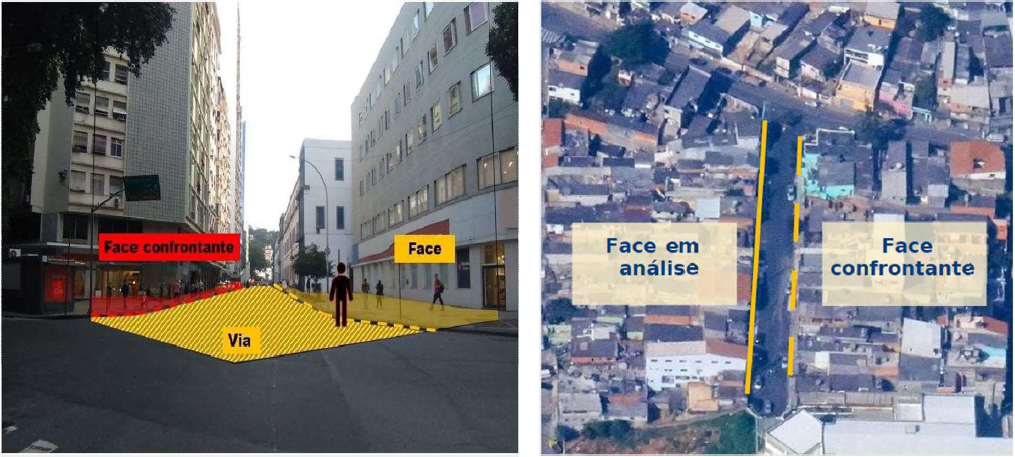
\includegraphics[keepaspectratio]{img/11-entorno/face.png}}

}

\end{figure}%

A definição de face não exige a presença de edificações, e é aí que
aparece uma situação que o leitor precisa ter em mente ao interpretar os
dados. Quando a face percorrida ou a confrontante corresponde ao limite
de um espaço não edificado, como um parque, uma praça ou a orla de uma
praia, não há fachadas para servir de alinhamento. Nesses casos, o IBGE
orientou que fossem considerados os itens avistados pelo agente enquanto
percorria o caminho adjacente ao espaço observado, de modo que a área de
análise passa a ser a calçada somada ao \textbf{campo de visão} do
agente (IBGE, 2025a). A Figura~\ref{fig-face-nao-edificada} ilustra as
duas situações.

\begin{figure}[H]

\caption{\label{fig-face-nao-edificada}Delimitação da área de observação
em faces que limitam espaços não edificados, com a área analisada
definida pelo campo de visão do agente. Fonte: IBGE (2025a).}

\centering{

\pandocbounded{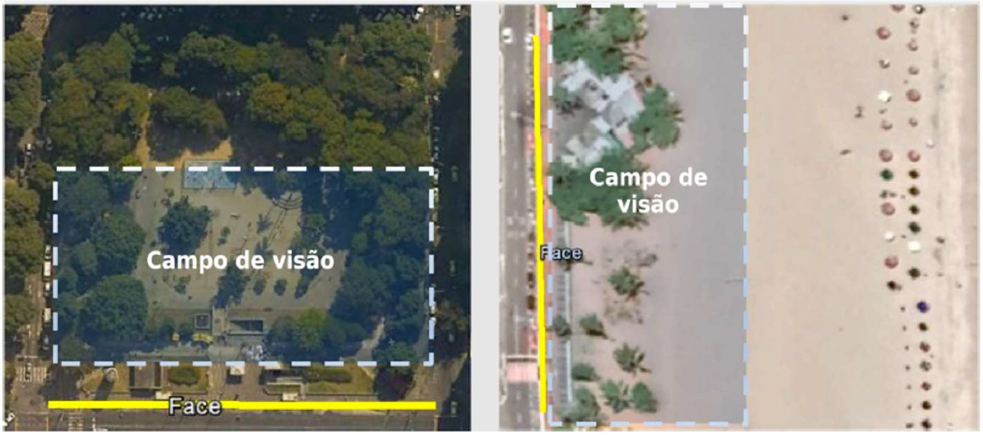
\includegraphics[keepaspectratio]{img/11-entorno/face-nao-edificavel.png}}

}

\end{figure}%

Duas implicações decorrem disso. A primeira é que faces sem nenhum
domicílio entram normalmente na contagem de faces do setor, o que ajuda
a explicar por que os percentuais calculados sobre faces e sobre
domicílios divergem, ponto que retomaremos na parte prática. A segunda é
que, nesses trechos, o registro depende de um julgamento visual do
agente sobre o que está ao alcance da vista, e não de um limite físico
bem definido.

\subsection{O universo da pesquisa}\label{sec-entorno-universo}

A Pesquisa Urbanística não cobre o país inteiro, e entender quem fica de
fora é pré-requisito para interpretar qualquer percentual calculado a
partir dela. Em 2010, o critério era a existência de arruamento regular.
Setores rurais e setores urbanos sem quadras e faces identificáveis
ficaram fora da pré-coleta (IBGE, 2012). Em 2022, o critério passou a
ser a \textbf{morfologia urbana observada}, e não a classificação legal
do setor. Além dos setores classificados como urbanos na Base
Territorial, entraram setores com áreas urbanizadas mapeadas e setores
que apresentassem concentração de estruturas, edificações e equipamentos
urbanos ou sistema viário consolidado, independentemente de serem
urbanos ou rurais. A identificação desses casos adicionais foi feita por
análise de imagens de satélite de alta resolução (IBGE, 2025a). Nos
setores rurais com pequenos núcleos de morfologia urbana ou situados em
franja periurbana, a pesquisa alcançou apenas a porção urbanizada, onde
havia faces definidas.

O resultado é uma cobertura alta dentro do universo escolhido e parcial
em relação ao país. Em 2022, dos 202.083.020 moradores de domicílios
particulares permanentes enumerados pelo Censo, 174.162.485 residiam em
setores selecionados para a pesquisa, o equivalente a 86,2\%. Dentro
desses setores, a coleta alcançou 99,7\% dos domicílios particulares
permanentes ocupados, com variação entre 99,5\% no Rio de Janeiro e em
Rondônia e 100,0\% no Amapá (IBGE, 2025a). Em 2010, a pesquisa alcançou
96,9\% dos domicílios particulares permanentes \textbf{urbanos} do país,
com variação regional entre 94,7\% no Nordeste e 99,7\% no Centro-Oeste
(IBGE, 2012).

\begin{tcolorbox}[enhanced jigsaw, arc=.35mm, bottomrule=.15mm, bottomtitle=1mm, breakable, colback=white, colbacktitle=quarto-callout-warning-color!10!white, colframe=quarto-callout-warning-color-frame, coltitle=black, left=2mm, leftrule=.75mm, opacityback=0, opacitybacktitle=0.6, rightrule=.15mm, title=\textcolor{quarto-callout-warning-color}{\faExclamationTriangle}\hspace{0.5em}{Os percentuais do entorno não são percentuais do Brasil}, titlerule=0mm, toprule=.15mm, toptitle=1mm]

Quando este capítulo disser que determinado percentual de domicílios
está em faces com calçada, o denominador serão sempre os domicílios
\textbf{do universo da pesquisa} (ou seja, o total que teve suas
características do entorno investigadas), e não todos os domicílios do
município, do estado ou do país. Essa ressalva vale para 2010 e para
2022, com recortes de universo diferentes em cada ano.

\end{tcolorbox}

\subsection{O questionário e o momento da
coleta}\label{sec-entorno-questionario}

Como visto na Seção~\ref{sec-produtos_censo}, a Pesquisa Urbanística
corresponde à etapa de reconhecimento do setor censitário, anterior à
coleta domiciliar. Antes de tratar de quem executou essa etapa e quando,
vale conhecer o próprio instrumento, reproduzido na
Figura~\ref{fig-questionario}.

\begin{figure}[H]

\caption{\label{fig-questionario}Questionário da Pesquisa Urbanística do
Entorno dos Domicílios aplicado no Censo Demográfico 2022. Fonte: IBGE
(2025a).}

\centering{

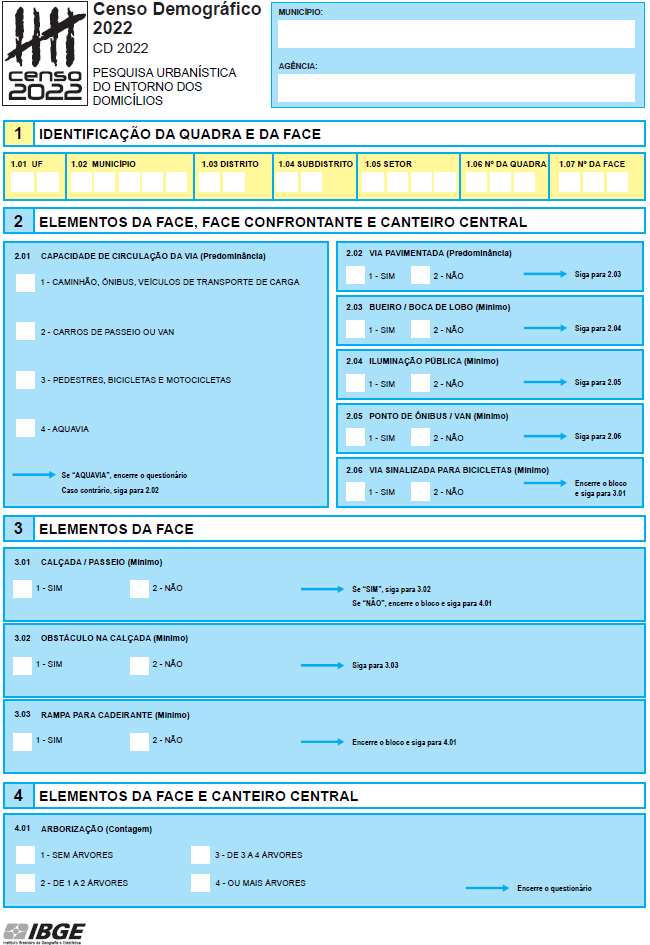
\includegraphics[width=0.88\linewidth,height=\textheight,keepaspectratio]{img/11-entorno/quest-entorno.png}

}

\end{figure}%

O questionário cabe em uma única página e está organizado em quatro
blocos. O bloco 1 apenas identifica a quadra e a face dentro do setor
censitário. Os três seguintes agrupam os itens pelo \textbf{elemento que
precisa ser observado} (face, canteiro central ou face confrontante)
para respondê-los. Repare ainda em dois detalhes que o questionário
revela de imediato. Ao lado de cada item aparece, entre parênteses, o
critério que rege o registro, com as indicações de \emph{Predominância},
\emph{Mínimo} e \emph{Contagem}. Já as setas azuis à direita explicitam
o encadeamento das perguntas, incluindo as instruções de encerrar o
questionário ou pular um bloco inteiro.

Quanto ao calendário da coleta, há consequências analíticas que convém
registrar. Em 2010, a operação de pré-coleta começou em 12 de abril para
os municípios com mais de 1.500 endereços residenciais urbanos e em 7 de
maio para os demais, estendendo-se até junho. Uma parte residual do
levantamento foi realizada já durante a coleta do Censo, iniciada em
agosto de 2010, em setores com características mistas de regularidade e
irregularidade urbanas (IBGE, 2012). Em 2022, a coleta se deu
prioritariamente na etapa de Reconhecimento do Setor Censitário, entre
20 de junho e 31 de julho, complementada por duas frentes. Durante as
entrevistas domiciliares, os recenseadores puderam ajustar as
informações registradas pelos agentes supervisores e indicar a inclusão
de novas faces. Já a etapa conhecida como \textbf{Entorno pós-coleta}
atendeu setores em que a pesquisa não pôde ser feita antes por razões
logísticas, além das localidades de povos e comunidades tradicionais em
áreas urbanas, onde se garantiu que o primeiro contato do IBGE com as
lideranças fosse a reunião de abordagem do recenseador (IBGE, 2025a).

Daí decorre uma característica que merece atenção. As informações do
entorno têm como referência a \textbf{data efetiva da observação em
campo}, enquanto os questionários domiciliares têm como referência a
meia-noite de 31 de julho para 1º de agosto. Entorno e domicílio de um
mesmo setor, portanto, não são estritamente contemporâneos. Em 2022,
embora a maior parte da coleta se concentre em pouco mais de um mês (20
de junho a 31 de julho de 2022), o período a que se referem as
informações do entorno estende-se de 20 de junho de 2022 a 28 de maio de
2023 (IBGE, 2025a). Em 2010 a defasagem também alcançava alguns meses,
já que a pré-coleta antecedeu em cerca de um trimestre a data de
referência do censo.

Três situações de campo fogem do padrão e explicam feições que o leitor
encontrará nos dados. A primeira ocorre em favelas e comunidades urbanas
muito adensadas, onde a ocorrência de faces era inexistente ou
rarefeita. Nesses casos, a coleta se deu por captura de coordenadas
geográficas, com um questionário aplicado a cada quinze edificações
visíveis ao longo do percurso. A segunda é a inclusão de faces novas por
rastreio\footnote{\emph{tracking}} georreferenciado, quando o mapa não
correspondia ao encontrado em campo. A terceira é o Distrito Federal,
cuja estrutura de quadras exigiu duas metodologias específicas,
denominadas Blocos Superquadras e Faces-quadras, além das faces
tradicionais, que seguem o padrão nacional (IBGE, 2025a).

\subsubsection{Critérios de análise e área de
observação}\label{sec-entorno-criterios}

Chegamos ao ponto que mais afeta a interpretação dos resultados. Os dez
itens de 2022 não foram registrados da mesma maneira. Cada um combina um
\textbf{critério de análise}, que define o que basta para considerar o
item existente, com um \textbf{local de investigação}, que define até
onde vai o olhar do agente. Os três critérios são os seguintes.

\begin{itemize}
\tightlist
\item
  \textbf{Mínimo}, quando basta observar a existência do item em
  qualquer ponto da área analisada. Foi o critério de sete dos dez
  itens.
\item
  \textbf{Contagem}, quando foi preciso quantificar o elemento
  observado. Aplicou-se apenas à arborização, registrada em quatro
  classes.
\item
  \textbf{Predominância}, quando a característica precisava ser
  preponderante, ou seja, estar presente em mais de 50\% do trecho.
  Aplicou-se à capacidade de circulação da via e à pavimentação.
\end{itemize}

A Tabela~\ref{tbl-criterios} cruza esses critérios com a área observada
em cada item.

\begin{longtable}[t]{lll}

\caption{\label{tbl-criterios}Critério de análise e local de
investigação de cada item da Pesquisa Urbanística do Entorno dos
Domicílios no Censo 2022.}

\tabularnewline

\toprule
Quesito & Critério & Local de investigação\\
\midrule
Capacidade de circulação da via & Predominância (mais de 50\%) & Face, face confrontante e canteiro central\\
Pavimentação da via & Predominância (mais de 50\%) & Face, face confrontante e canteiro central\\
Bueiro ou boca de lobo & Mínimo & Face, face confrontante e canteiro central\\
Iluminação pública & Mínimo & Face, face confrontante e canteiro central\\
Ponto de ônibus ou van & Mínimo & Face, face confrontante e canteiro central\\
\addlinespace
Via sinalizada para bicicletas & Mínimo & Face, face confrontante e canteiro central\\
Calçada ou passeio & Mínimo & Somente a face percorrida\\
Obstáculo na calçada & Mínimo & Somente a face percorrida\\
Rampa para cadeirante & Mínimo & Somente a face percorrida\\
Arborização & Contagem (0, 1 a 2, 3 a 4, 5+) & Face percorrida e canteiro central\\
\bottomrule

\end{longtable}

São três as consequências principais. Primeiro, os itens ligados à
calçada olham \textbf{apenas para a face percorrida}, enquanto os itens
ligados à via olham para os dois lados. Um percentual de calçadas e um
percentual de iluminação, ainda que apresentados lado a lado, não
descrevem a mesma extensão de espaço público. Segundo, a arborização é o
único item que considera a face e o canteiro central sem considerar a
face confrontante, escolha que, como veremos adiante, inviabiliza a
comparação com 2010. Por fim, a pesquisa investiga \textbf{existência,
não estado de conservação, funcionamento ou eficácia} (IBGE, 2025a). Um
poste sem lâmpada conta como iluminação pública existente. Um bueiro
entupido conta como bueiro existente. Os dados descrevem a presença do
equipamento urbano, e não a sua qualidade.

\subsubsection{O fluxo do questionário e seus
saltos}\label{sec-entorno-fluxo}

O questionário de 2022 possui uma lógica condicional que faz com que
certos itens deixem de ser aplicados em determinadas faces, e essa
lógica é a origem de uma categoria de resposta que confunde muitos
usuários dos dados. Há dois saltos, ambos visíveis nas instruções
impressas na Figura~\ref{fig-questionario}. O primeiro ocorre quando a
capacidade de circulação da via é registrada como \textbf{aquavia},
situação em que o rio ou canal constitui a própria face e é a forma de
acesso direto às edificações. O formulário instrui a encerrar o
questionário ali mesmo, e nenhum outro item é preenchido. O segundo,
muito mais frequente, ocorre quando \textbf{não há calçada} na face.
Como obstáculo e rampa são características da calçada, não faz sentido
investigá-los onde ela não existe, e o item 3.01 manda seguir direto
para o bloco de arborização. A Figura~\ref{fig-fluxo-questionario}
resume esse encadeamento.

\begin{figure}[H]

\caption{\label{fig-fluxo-questionario}Fluxo do questionário da Pesquisa
Urbanística do Entorno dos Domicílios no Censo 2022, com os dois pontos
de salto. Elaborado a partir do questionário reproduzido na
Figura~\ref{fig-questionario}.}

\centering{

\includegraphics[width=6.5in,height=12.37in]{11-entorno_files/figure-latex/mermaid-figure-1.png}

}

\end{figure}%

Guarde este fluxograma, pois quando chegarmos aos dados, veremos que as
faces que sofreram ``salto'' não desaparecem das tabelas. Elas são
contabilizadas em categorias específicas de não resposta, e confundi-las
com falhas de coleta produz percentuais errados.

\subsection{As variáveis e sua
disponibilização}\label{sec-entorno-variaveis}

É importante salientar que as tabelas de 2010 e de 2022 \textbf{não
diferem apenas nos itens investigados}. Elas têm arquiteturas
incompatíveis, e quem tentar transportar o raciocínio de um ano para o
outro vai errar. Vejamos cada uma.

\subsubsection{Variáveis do Censo 2022}\label{sec-entorno-var2022}

A tabela de 2022 organiza a informação em três blocos que medem os
mesmos dez itens em \textbf{unidades de contagem diferentes}. O primeiro
conta faces de quadra, ou seja, o dado como foi coletado. O segundo
conta domicílios particulares permanentes ocupados situados naquelas
faces. O terceiro conta os moradores desses domicílios. A
Tabela~\ref{tbl-blocos-2022} resume a estrutura, já usando os nomes que
o pacote \texttt{censobr} atribui às colunas.

\begin{longtable}[t]{cccc}

\caption{\label{tbl-blocos-2022}Blocos de variáveis do arquivo Entorno
do Censo 2022 e suas respectivas variáveis de total.}

\tabularnewline

\toprule
Bloco & Prefixo no censobr & Variável de total & Unidade contada\\
\midrule
Faces de quadra & faces\_V054xx & faces\_V05400 & Faces com questionário aplicado\\
Domicílios & domicilios\_V050xx & domicilios\_V05000 & Domicílios particulares permanentes ocupados com entorno pesquisado\\
Moradores & moradores\_V052xx & moradores\_V05200 & Moradores desses domicílios\\
\bottomrule

\end{longtable}

Os três blocos têm 35 variáveis cada e seguem exatamente o mesmo
\emph{layout}, com os itens na mesma ordem e na mesma posição relativa à
variável de total. A existência de bueiro, por exemplo, ocupa o nono
deslocamento nos três blocos, em \texttt{faces\_V05409},
\texttt{domicilios\_V05009} e \texttt{moradores\_V05209}\footnote{Essa
  regularidade é uma boa notícia para quem programa, porque permite
  escrever uma única rotina que atende aos três blocos.}.

Dentro de cada bloco, os itens aparecem decompostos em categorias. Oito
deles trazem a tríade \textbf{Sim}, \textbf{Não} e \textbf{Não
Declarado}. Os dois restantes trazem classes múltiplas, pois a
arborização é registrada em quatro faixas de contagem e a capacidade de
circulação da via em quatro tipos de veículo, e ambos contam ainda com
uma categoria reservada aos casos em que o item não chegou a ser
perguntado. A propriedade que torna o cálculo simples é que, em todo
item, \textbf{as categorias somam a variável de total do bloco}. O
denominador de um percentual, portanto, é sempre a variável de total, e
não uma soma que o analista precise montar.

Por outro lado, essa simplicidade é compensada pela existência da
categoria ``Não Declarado'', que carrega dois significados distintos. Na
maioria dos itens ela reúne um resíduo pequeno de inconsistências e não
validações. Nos itens de obstáculo na calçada e rampa para cadeirante,
ela absorve também as faces que sofreram o ``salto'' do questionário, ou
seja, aquelas em que não existe calçada. O que parece uma não resposta
é, na verdade, um ``não se aplica''. Voltaremos a esse ponto com números
na parte prática, porque ele muda o resultado de forma perceptível.

\subsubsection{Variáveis do Censo 2010}\label{sec-entorno-var2010}

A organização dos dados de 2010 segue uma outra lógica. São 1.161
variáveis distribuídas em cinco arquivos, de \texttt{Entorno01} a
\texttt{Entorno05}, e três diferenças estruturais a separam de 2022. A
primeira é que \textbf{não existe contagem de faces}. Embora a coleta
tenha sido feita por face, o produto divulgado conta apenas domicílios e
moradores. Não há como saber, em 2010, qual proporção das faces de um
setor tinha calçada. A segunda é que \textbf{não existe a categoria
``Não Declarado''}, já que cada item aparece apenas como ``Existe'' ou
``Não existe''.

A terceira é a mais complexa para quem abre o arquivo pela primeira vez.
Em 2010, os itens do entorno \textbf{nunca aparecem sozinhos}. Eles vêm
sempre cruzados com um atributo do domicílio ou do morador. Não há uma
variável que informe quantos domicílios estão em faces com iluminação
pública. Há variáveis que informam quantos domicílios \emph{próprios}
estão em faces com iluminação, quantos \emph{alugados}, quantos
\emph{com responsável do sexo feminino}, quantos \emph{de renda per
capita até um quarto de salário mínimo}, e assim por diante. O arquivo
é, na prática, uma coleção de tabulações cruzadas (IBGE, 2011).

Essa organização em blocos gera uma complexidade prática, pois como não
há uma variável de total de domicílios com entorno pesquisado, o
denominador precisa ser reconstruído somando um bloco inteiro. E
\textbf{nem todos os blocos são exaustivos}. Os blocos de condição de
ocupação, de abastecimento de água e de existência de banheiro e
esgotamento sanitário deixam categorias de fora, de modo que somá-los
produz um total menor que o correto. Já os blocos de sexo do
responsável, adequação da moradia, renda per capita, grupos de idade e
cor ou raça cobrem todos os domicílios ou moradores pesquisados. A
escolha do bloco de referência é, portanto, uma decisão metodológica
importante. Trataremos disso com código na parte prática.

A Tabela~\ref{tbl-estrutura} confronta estruturalmente os resultados do
Entorno para ambos os censos e sintetiza o que muda de um censo para o
outro.

\begin{longtable}[t]{ccc}

\caption{\label{tbl-estrutura}Diferenças estruturais entre os arquivos
de entorno dos Censos de 2010 e 2022.}

\tabularnewline

\toprule
Aspecto & Censo 2010 & Censo 2022\\
\midrule
Contagem de faces & Ausente & Presente, em bloco próprio\\
Unidades de contagem & Domicílios e moradores & Faces, domicílios e moradores\\
Categorias de resposta & Existe e Não existe & Sim, Não e Não Declarado\\
Total de pesquisados & Não divulgado, precisa ser reconstruído & Variável explícita em cada bloco\\
Forma de apresentação & Sempre cruzado com atributo do domicílio ou morador & Item isolado\\
\addlinespace
Número de variáveis & 1.161, em cinco arquivos & 105, em um arquivo\\
Itens com classes múltiplas & Nenhum & Arborização e capacidade da via\\
\bottomrule

\end{longtable}

Para entender o que é possível ou não comparar, vale mencionar que seis
itens aparecem nos dois censos, o que sugere uma série histórica
confortável. No entanto, a realidade é bem mais restrita, já que o
próprio IBGE alerta que apenas \textbf{dois} itens admitem comparação
direta, e a Tabela~\ref{tbl-comparabilidade} explica o motivo caso a
caso.

\begin{longtable}[t]{ccc}

\caption{\label{tbl-comparabilidade}Comparabilidade dos itens
investigados nos Censos de 2010 e 2022. Elaborado a partir da Tabela 2
de IBGE (2025a).}

\tabularnewline

\toprule
Quesito & Comparável? & Motivo\\
\midrule
Iluminação pública & Sim & Mesmo conceito e mesmo critério de coleta nos dois censos\\
Bueiro ou boca de lobo & Sim & Mesmo conceito e mesmo critério de coleta nos dois censos\\
Rampa para cadeirante & Com ressalva & Em 2010 foi investigada em todas as faces e em 2022 apenas nas faces com calçada\\
Calçada ou passeio & Não & Em 2010 exigia caminho calçado ou pavimentado e em 2022 aceita calçada sem pavimentação\\
Pavimentação da via & Não & Em 2010 bastava qualquer trecho pavimentado e em 2022 exige-se predominância\\
\addlinespace
Arborização & Não & Em 2010 considerava a face confrontante e em 2022 considera apenas a face e o canteiro central\\
\bottomrule

\end{longtable}

Note que as três incomparabilidades apontam em direções previsíveis. A
mudança no conceito de calçada tende a \textbf{inflar} o resultado de
2022, porque o conceito ficou mais abrangente. As mudanças em
pavimentação e arborização tendem a \textbf{reduzi-lo}, porque o
critério ficou mais exigente em um caso e a área observada diminuiu no
outro. Uma queda aparente na arborização entre 2010 e 2022 pode ser
inteiramente artefato metodológico.

\begin{tcolorbox}[enhanced jigsaw, arc=.35mm, bottomrule=.15mm, bottomtitle=1mm, breakable, colback=white, colbacktitle=quarto-callout-warning-color!10!white, colframe=quarto-callout-warning-color-frame, coltitle=black, left=2mm, leftrule=.75mm, opacityback=0, opacitybacktitle=0.6, rightrule=.15mm, title=\textcolor{quarto-callout-warning-color}{\faExclamationTriangle}\hspace{0.5em}{O universo também mudou, e isso independe dos itens}, titlerule=0mm, toprule=.15mm, toptitle=1mm]

Mesmo nos dois itens comparáveis, a comparação exige cautela adicional.
O número de setores pesquisados passou de 223.666 em 2010 para 340.965
em 2022\footnotemark{}, crescimento de mais de 50\% que decorre da
expansão das cidades e, principalmente, da decisão de incluir áreas
urbanizadas de setores rurais e setores de favelas e comunidades urbanas
(IBGE, 2025a). Como essas áreas incorporadas tendem a apresentar
infraestrutura mais precária, um percentual nacional que fique estável
entre os dois censos pode estar escondendo uma melhora real, e uma piora
aparente pode refletir apenas o alargamento do universo. Comparações por
recortes territoriais estáveis são sempre preferíveis às comparações de
médias nacionais.

\end{tcolorbox}

\footnotetext{Esse total de 2010 é o que consta na Tabela 3 de IBGE
(2025a). A publicação original de 2010 informa 222.541 setores (IBGE,
2012), diferença de pouco mais de mil setores que provavelmente decorre
de revisões posteriores da base territorial. A ordem de grandeza da
comparação não se altera.}

\subsection{Níveis geográficos de coleta e de
divulgação}\label{sec-entorno-niveis}

Neste ponto, é importante esclarecer um aspecto bastante relevante sobre
o produto: \textbf{a coleta ocorre na face, mas a divulgação é feita no
nível do setor censitário}. Isso quer dizer que a face de quadra é a
unidade de investigação, mas não é unidade de divulgação. Não existe, no
conjunto de dados públicos, uma tabela que informe as características
urbanísticas de uma face específica. O que se publica é a
\textbf{contagem de faces por categoria dentro de cada setor
censitário}, que passa a ser a maior resolução espacial disponível. Essa
diferença tem uma implicação analítica que convém fixar desde já, pois o
valor de um setor é uma síntese de faces que podem ser bastante
heterogêneas entre si.

A partir do setor censitário, a informação pode ser agregada para os
recortes já discutidos na Seção~\ref{sec-recortes}, na sequência bairro,
subdistrito, distrito e município, e daí para concentração urbana,
unidade da federação, grande região e Brasil. A publicação de 2022
apresenta resultados até o nível de município e de concentração urbana,
além de uma leitura segundo a hierarquia urbana definida em Regiões de
Influência das Cidades (IBGE, 2025a).

Há três caminhos de acesso aos dados, com alcances distintos:

\begin{itemize}
\tightlist
\item
  \textbf{Agregados por Setor Censitário:} É o único caminho que chega
  ao setor e, por ser o mais desagregado espacialmente, é o que usaremos
  neste livro. Em 2022 as variáveis do entorno foram incorporadas ao
  conjunto dos Agregados. Em 2010 elas vinham em cinco planilhas por
  unidade da federação, de \texttt{Entorno01\_UF} a
  \texttt{Entorno05\_UF}, dentro do mesmo pacote. Nos dois casos, o
  acesso se dá pela função \texttt{read\_tracts()} do pacote
  \texttt{censobr} (Pereira \& Barbosa, 2023).
\item
  \textbf{SIDRA:} Oferece tabelas prontas até o nível de município e de
  concentração urbana, incluindo os indicadores de cobertura da
  pesquisa. É a via mais rápida para consultas pontuais, sem a
  flexibilidade da manipulação programática.
\item
  \textbf{Plataforma Geográfica Interativa (PGI):} Disponibiliza
  arquivos vetoriais e temas relacionados para \emph{download}, voltada
  a quem trabalha diretamente em ambiente de geoprocessamento.
\end{itemize}

Com o terreno conceitual preparado, podemos partir para os dados. Na
próxima seção obteremos os arquivos de entorno dos dois censos com o
\texttt{censobr}, montaremos os indicadores respeitando os denominadores
corretos de cada ano e levaremos os resultados ao mapa.

\section{Obtendo e integrando os dados}\label{sec-entorno-dados}

Usaremos \textbf{Fortaleza} como pano de fundo do restante do capítulo.
O ponto de partida é a leitura dos arquivos de entorno dos dois censos
com a função \texttt{read\_tracts()}, já apresentada no
Seção~\ref{sec-obtendo}. O argumento \texttt{dataset} recebe o valor
\texttt{"Entorno"}, e o retorno é um \emph{Dataset} do Arrow, e não um
\texttt{data.frame}. Isso importa porque o arquivo de 2022 tem quase 345
mil linhas e o de 2010 tem 310 mil, com mais de mil colunas no caso de
2010. Filtrar antes de materializar evita carregar o país inteiro na
memória.

\begin{Shaded}
\begin{Highlighting}[]
\CommentTok{\# Código IBGE de Fortaleza (CE)}
\NormalTok{cod\_for }\OtherTok{\textless{}{-}} \DecValTok{2304400}

\CommentTok{\# Os objetos abaixo ainda não são data.frames, e sim Datasets do Arrow}
\NormalTok{ent2010 }\OtherTok{\textless{}{-}} \FunctionTok{read\_tracts}\NormalTok{(}\AttributeTok{year =} \DecValTok{2010}\NormalTok{, }\AttributeTok{dataset =} \StringTok{"Entorno"}\NormalTok{)}
\NormalTok{ent2022 }\OtherTok{\textless{}{-}} \FunctionTok{read\_tracts}\NormalTok{(}\AttributeTok{year =} \DecValTok{2022}\NormalTok{, }\AttributeTok{dataset =} \StringTok{"Entorno"}\NormalTok{)}

\CommentTok{\# O filtro é aplicado antes do collect(), que só então traz os dados à memória}
\NormalTok{ent\_for2010 }\OtherTok{\textless{}{-}}\NormalTok{ ent2010 }\SpecialCharTok{|\textgreater{}}
  \FunctionTok{filter}\NormalTok{(code\_muni }\SpecialCharTok{==}\NormalTok{ cod\_for) }\SpecialCharTok{|\textgreater{}}
  \FunctionTok{collect}\NormalTok{()}

\NormalTok{ent\_for2022 }\OtherTok{\textless{}{-}}\NormalTok{ ent2022 }\SpecialCharTok{|\textgreater{}}
  \FunctionTok{filter}\NormalTok{(code\_muni }\SpecialCharTok{==}\NormalTok{ cod\_for) }\SpecialCharTok{|\textgreater{}}
  \FunctionTok{collect}\NormalTok{()}
\end{Highlighting}
\end{Shaded}

\begin{tcolorbox}[enhanced jigsaw, arc=.35mm, bottomrule=.15mm, bottomtitle=1mm, breakable, colback=white, colbacktitle=quarto-callout-note-color!10!white, colframe=quarto-callout-note-color-frame, coltitle=black, left=2mm, leftrule=.75mm, opacityback=0, opacitybacktitle=0.6, rightrule=.15mm, title=\textcolor{quarto-callout-note-color}{\faInfo}\hspace{0.5em}{Por que não existe
\texttt{read\_tracts(year\ =\ 2000,\ dataset\ =\ "Entorno")}}, titlerule=0mm, toprule=.15mm, toptitle=1mm]

Como registrado na Tabela~\ref{tbl-quesitos-censos}, o Censo 2000
investigou três itens do entorno, mas os divulgou vinculados ao
domicílio nos resultados da amostra, e não nos Agregados por Setor
Censitário. Por isso o \texttt{censobr} não oferece o conjunto
\texttt{Entorno} para aquele ano, e a chamada retorna erro. A série por
setor começa em 2010.

\end{tcolorbox}

Antes de qualquer cálculo, o dicionário precisa estar aberto ao lado. Já
se sabe dos capítulos anteriores que a função
\texttt{data\_dictionary()} cuida disso. Lembre-se que para 2010 ela
abre um PDF, e nele podemos verificar que as seções 6.22 a 6.26
descrevem os cinco arquivos de entorno. Já para 2022, a função abre uma
pasta de trabalho \texttt{.xlsx}, cuja última aba, chamada
\texttt{Entorno}, traz as variáveis que nos interessam.

\begin{Shaded}
\begin{Highlighting}[]
\FunctionTok{data\_dictionary}\NormalTok{(}\AttributeTok{year =} \DecValTok{2010}\NormalTok{, }\AttributeTok{dataset =} \StringTok{"tracts"}\NormalTok{)  }\CommentTok{\# abre um PDF}
\FunctionTok{data\_dictionary}\NormalTok{(}\AttributeTok{year =} \DecValTok{2022}\NormalTok{, }\AttributeTok{dataset =} \StringTok{"tracts"}\NormalTok{)  }\CommentTok{\# abre um .xlsx, ver aba "Entorno"}
\end{Highlighting}
\end{Shaded}

Recorde-se também que até a versão do \texttt{censobr} trabalhada no
nosso texto (v0.6.0), os arquivos não vêm com uma coluna de geometria.
Deste modo, precisamos obter os polígonos dos setores no \texttt{geobr},
com \texttt{read\_census\_tract()}. O argumento \texttt{code\_tract}
aceita o código do município para devolver todos os seus setores. Usamos
\texttt{simplified\ =\ FALSE} para preservar o traçado original.

\begin{Shaded}
\begin{Highlighting}[]
\NormalTok{geo\_for2010 }\OtherTok{\textless{}{-}} \FunctionTok{read\_census\_tract}\NormalTok{(}\AttributeTok{year =} \DecValTok{2010}\NormalTok{, }\AttributeTok{code\_tract =}\NormalTok{ cod\_for,}
                                 \AttributeTok{simplified =} \ConstantTok{FALSE}\NormalTok{)}
\NormalTok{geo\_for2022 }\OtherTok{\textless{}{-}} \FunctionTok{read\_census\_tract}\NormalTok{(}\AttributeTok{year =} \DecValTok{2022}\NormalTok{, }\AttributeTok{code\_tract =}\NormalTok{ cod\_for,}
                                 \AttributeTok{simplified =} \ConstantTok{FALSE}\NormalTok{)}
\end{Highlighting}
\end{Shaded}

\subsection{Nem todo setor tem dado de entorno}\label{sec-entorno-join}

Aqui aparece a primeira consequência prática da
Seção~\ref{sec-entorno-universo}. O \texttt{geobr} devolve
\textbf{todos} os setores do município, enquanto o arquivo de entorno
traz apenas os que entraram no universo da pesquisa. Um
\texttt{left\_join()} entre os dois produz valores ausentes, e é muito
melhor contá-los de forma deliberada do que descobri-los depois como
buracos inexplicados no mapa.

\begin{Shaded}
\begin{Highlighting}[]
\FunctionTok{tibble}\NormalTok{(}
  \AttributeTok{Censo =} \FunctionTok{c}\NormalTok{(}\DecValTok{2010}\NormalTok{, }\DecValTok{2022}\NormalTok{),}
  \StringTok{\textasciigrave{}}\AttributeTok{Setores na malha}\StringTok{\textasciigrave{}} \OtherTok{=} \FunctionTok{c}\NormalTok{(}\FunctionTok{nrow}\NormalTok{(geo\_for2010), }\FunctionTok{nrow}\NormalTok{(geo\_for2022)),}
  \StringTok{\textasciigrave{}}\AttributeTok{Setores no Entorno}\StringTok{\textasciigrave{}} \OtherTok{=} \FunctionTok{c}\NormalTok{(}\FunctionTok{nrow}\NormalTok{(ent\_for2010), }\FunctionTok{nrow}\NormalTok{(ent\_for2022)),}
  \StringTok{\textasciigrave{}}\AttributeTok{Sem correspondência}\StringTok{\textasciigrave{}} \OtherTok{=} \FunctionTok{c}\NormalTok{(}
    \FunctionTok{sum}\NormalTok{(}\SpecialCharTok{!}\NormalTok{geo\_for2010}\SpecialCharTok{$}\NormalTok{code\_tract }\SpecialCharTok{\%in\%}\NormalTok{ ent\_for2010}\SpecialCharTok{$}\NormalTok{code\_tract),}
    \FunctionTok{sum}\NormalTok{(}\SpecialCharTok{!}\NormalTok{geo\_for2022}\SpecialCharTok{$}\NormalTok{code\_tract }\SpecialCharTok{\%in\%}\NormalTok{ ent\_for2022}\SpecialCharTok{$}\NormalTok{code\_tract)}
\NormalTok{  )}
\NormalTok{) }\SpecialCharTok{|\textgreater{}}
\NormalTok{  knitr}\SpecialCharTok{::}\FunctionTok{kable}\NormalTok{(}\AttributeTok{align =} \FunctionTok{c}\NormalTok{(}\StringTok{"c"}\NormalTok{, }\StringTok{"c"}\NormalTok{, }\StringTok{"c"}\NormalTok{, }\StringTok{"c"}\NormalTok{),}
               \AttributeTok{format.args =} \FunctionTok{list}\NormalTok{(}\AttributeTok{big.mark =} \StringTok{"."}\NormalTok{, }\AttributeTok{decimal.mark =} \StringTok{","}\NormalTok{)) }\SpecialCharTok{|\textgreater{}}
\NormalTok{  kableExtra}\SpecialCharTok{::}\FunctionTok{kable\_styling}\NormalTok{(}\AttributeTok{full\_width =} \ConstantTok{FALSE}\NormalTok{)}
\end{Highlighting}
\end{Shaded}

\begin{longtable}[t]{cccc}

\caption{\label{tbl-entorno-cobertura}Setores censitários de Fortaleza
disponíveis na malha do \texttt{geobr} e no arquivo de entorno do
\texttt{censobr}, nos dois censos.}

\tabularnewline

\toprule
Censo & Setores na malha & Setores no Entorno & Sem correspondência\\
\midrule
2.010 & 3.043 & 3.020 & 23\\
2.022 & 4.408 & 4.381 & 27\\
\bottomrule

\end{longtable}

Os 23 setores de 2010 e os 27 de 2022 que ficam sem par são setores que
não foram selecionados para a pesquisa, \textbf{não consistindo em falha
de dado}. Eles aparecerão nos mapas com a cor reservada a valores
ausentes. Repare também que a malha de Fortaleza cresceu de 3.043 para
4.408 setores entre os dois censos, informação que será decisiva na
Seção~\ref{sec-entorno-comparacao}.

Em 2022 existe ainda um segundo tipo de ausência, mais sutil, que não
vem do \texttt{join} e sim do próprio arquivo. Abaixo, contabilizamos a
quantidade de setores que possuem \texttt{NA} na variável de total de
domicílios investigados com relação ao entorno:

\begin{Shaded}
\begin{Highlighting}[]
\FunctionTok{sum}\NormalTok{(}\FunctionTok{is.na}\NormalTok{(ent\_for2022}\SpecialCharTok{$}\NormalTok{domicilios\_V05000))}
\end{Highlighting}
\end{Shaded}

\begin{verbatim}
[1] 111
\end{verbatim}

São 111 setores com faces pesquisadas mas sem total de domicílios,
tipicamente setores sem uso residencial, como grandes áreas de parque,
equipamentos e concentrações de comércio. A consequência direta é que
\textbf{um indicador calculado sobre faces existe nesses setores,
enquanto o mesmo indicador calculado sobre domicílios não existe.}
Somando os 27 setores não pareados aos 111 sem domicílios, um mapa por
domicílios terá 138 setores em branco, contra apenas 27 de um mapa por
faces.

\section{A escolha do denominador}\label{sec-entorno-denominador}

A Seção~\ref{sec-entorno-var2022} estabeleceu a regra de cálculo de
2022, ou seja, as categorias de todo item somam a variável de total do
bloco, de modo que o denominador é sempre essa variável. O que a regra
não resolve é a pergunta anterior a ela, que é decidir \textbf{qual
bloco usar}. Vamos medir os mesmos itens nas duas unidades e comparar.

\begin{Shaded}
\begin{Highlighting}[]
\CommentTok{\# Função auxiliar para calcular percentuais com segurança. Se a variável de}
\CommentTok{\# total (o denominador) for 0 ou ausente, ela é substituída por NA\_real\_, e a}
\CommentTok{\# divisão 100 * numerador / total devolve NA em vez de Inf ou NaN. Aqui, com}
\CommentTok{\# totais municipais, isso nunca acontece, mas será decisivo nos cálculos por}
\CommentTok{\# setor logo adiante, onde há os 111 setores sem domicílios investigados.}
\NormalTok{perc }\OtherTok{\textless{}{-}} \ControlFlowTok{function}\NormalTok{(numerador, total) \{}
\NormalTok{  total }\OtherTok{\textless{}{-}} \FunctionTok{ifelse}\NormalTok{(}\FunctionTok{is.na}\NormalTok{(total) }\SpecialCharTok{|}\NormalTok{ total }\SpecialCharTok{==} \DecValTok{0}\NormalTok{, }\ConstantTok{NA\_real\_}\NormalTok{, total)}
  \DecValTok{100} \SpecialCharTok{*}\NormalTok{ numerador }\SpecialCharTok{/}\NormalTok{ total}
\NormalTok{\}}

\CommentTok{\# Totais municipais de cada variável dos três blocos}
\CommentTok{\# Obs.: mais explicações sobre as funções novas que aparecem abaixo na nota mais adiante.}
\NormalTok{tot\_for2022 }\OtherTok{\textless{}{-}}\NormalTok{ ent\_for2022 }\SpecialCharTok{|\textgreater{}}
  \FunctionTok{summarize}\NormalTok{(}\FunctionTok{across}\NormalTok{(}\FunctionTok{starts\_with}\NormalTok{(}\FunctionTok{c}\NormalTok{(}\StringTok{"faces\_"}\NormalTok{, }\StringTok{"domicilios\_"}\NormalTok{)),}
\NormalTok{                   \textbackslash{}(x) }\FunctionTok{sum}\NormalTok{(x, }\AttributeTok{na.rm =} \ConstantTok{TRUE}\NormalTok{)))}

\FunctionTok{tibble}\NormalTok{(}
  \AttributeTok{Item =} \FunctionTok{c}\NormalTok{(}\StringTok{"Via pavimentada"}\NormalTok{, }\StringTok{"Iluminação pública"}\NormalTok{,}
           \StringTok{"Bueiro ou boca de lobo"}\NormalTok{, }\StringTok{"Calçada ou passeio"}\NormalTok{,}
           \StringTok{"Ponto de ônibus ou van"}\NormalTok{, }\StringTok{"Via sinalizada para bicicletas"}\NormalTok{,}
           \StringTok{"Rampa para cadeirante"}\NormalTok{, }\StringTok{"Sem árvores"}\NormalTok{),}
  \AttributeTok{face =} \FunctionTok{c}\NormalTok{(}\StringTok{"faces\_V05406"}\NormalTok{, }\StringTok{"faces\_V05412"}\NormalTok{,}
           \StringTok{"faces\_V05409"}\NormalTok{, }\StringTok{"faces\_V05421"}\NormalTok{,}
           \StringTok{"faces\_V05415"}\NormalTok{, }\StringTok{"faces\_V05418"}\NormalTok{,}
           \StringTok{"faces\_V05427"}\NormalTok{, }\StringTok{"faces\_V05430"}\NormalTok{),}
  \AttributeTok{domicilio =} \FunctionTok{c}\NormalTok{(}\StringTok{"domicilios\_V05006"}\NormalTok{, }\StringTok{"domicilios\_V05012"}\NormalTok{,}
                \StringTok{"domicilios\_V05009"}\NormalTok{, }\StringTok{"domicilios\_V05021"}\NormalTok{,}
                \StringTok{"domicilios\_V05015"}\NormalTok{, }\StringTok{"domicilios\_V05018"}\NormalTok{,}
                \StringTok{"domicilios\_V05027"}\NormalTok{, }\StringTok{"domicilios\_V05030"}\NormalTok{)}
\NormalTok{) }\SpecialCharTok{|\textgreater{}}
  \FunctionTok{mutate}\NormalTok{(}
    \StringTok{\textasciigrave{}}\AttributeTok{\% das faces}\StringTok{\textasciigrave{}}      \OtherTok{=} \FunctionTok{perc}\NormalTok{(}\FunctionTok{as.numeric}\NormalTok{(tot\_for2022[face]),}
\NormalTok{                              tot\_for2022}\SpecialCharTok{$}\NormalTok{faces\_V05400),}
    \StringTok{\textasciigrave{}}\AttributeTok{\% dos domicílios}\StringTok{\textasciigrave{}} \OtherTok{=} \FunctionTok{perc}\NormalTok{(}\FunctionTok{as.numeric}\NormalTok{(tot\_for2022[domicilio]),}
\NormalTok{                              tot\_for2022}\SpecialCharTok{$}\NormalTok{domicilios\_V05000),}
    \AttributeTok{face =} \ConstantTok{NULL}\NormalTok{, }\AttributeTok{domicilio =} \ConstantTok{NULL}
\NormalTok{  ) }\SpecialCharTok{|\textgreater{}}
\NormalTok{  knitr}\SpecialCharTok{::}\FunctionTok{kable}\NormalTok{(}\AttributeTok{digits =} \DecValTok{1}\NormalTok{, }\AttributeTok{align =} \FunctionTok{c}\NormalTok{(}\StringTok{"l"}\NormalTok{, }\StringTok{"c"}\NormalTok{, }\StringTok{"c"}\NormalTok{),}
               \AttributeTok{format.args =} \FunctionTok{list}\NormalTok{(}\AttributeTok{decimal.mark =} \StringTok{","}\NormalTok{)) }\SpecialCharTok{|\textgreater{}}
\NormalTok{  kableExtra}\SpecialCharTok{::}\FunctionTok{kable\_styling}\NormalTok{(}\AttributeTok{full\_width =} \ConstantTok{FALSE}\NormalTok{)}
\end{Highlighting}
\end{Shaded}

\begin{longtable}[t]{lcc}

\caption{\label{tbl-entorno-unidades}Os mesmos itens do entorno medidos
sobre faces de quadra e sobre domicílios, Fortaleza (Censo 2022).}

\tabularnewline

\toprule
Item & \% das faces & \% dos domicílios\\
\midrule
Via pavimentada & 88,6 & 93,9\\
Iluminação pública & 96,3 & 99,0\\
Bueiro ou boca de lobo & 28,4 & 33,1\\
Calçada ou passeio & 79,5 & 89,0\\
Ponto de ônibus ou van & 10,5 & 12,0\\
\addlinespace
Via sinalizada para bicicletas & 7,9 & 7,2\\
Rampa para cadeirante & 10,1 & 12,2\\
Sem árvores & 49,0 & 39,8\\
\bottomrule

\end{longtable}

\begin{tcolorbox}[enhanced jigsaw, arc=.35mm, bottomrule=.15mm, bottomtitle=1mm, breakable, colback=white, colbacktitle=quarto-callout-note-color!10!white, colframe=quarto-callout-note-color-frame, coltitle=black, left=2mm, leftrule=.75mm, opacityback=0, opacitybacktitle=0.6, rightrule=.15mm, title=\textcolor{quarto-callout-note-color}{\faInfo}\hspace{0.5em}{Três novidades de sintaxe no código acima}, titlerule=0mm, toprule=.15mm, toptitle=1mm]

\begin{itemize}
\tightlist
\item
  \textbf{\texttt{across()}} aplica a mesma operação a várias colunas de
  uma só vez, dentro de um \texttt{summarize()} ou de um
  \texttt{mutate()}. Sem ela, seria preciso escrever uma linha de
  \texttt{sum()} para cada uma das 70 variáveis dos blocos de faces e de
  domicílios.
\item
  \textbf{\texttt{starts\_with()}} é uma das funções de seleção auxiliar
  do \texttt{tidyselect}, que escolhe colunas por padrão no nome. Aqui
  ela captura de uma vez todas as colunas iniciadas por \texttt{faces\_}
  e por \texttt{domicilios\_}. Existem outras da mesma família, como
  \texttt{ends\_with()}, \texttt{contains()} e \texttt{all\_of()}, esta
  última usada mais adiante neste capítulo.
\item
  \textbf{\texttt{\textbackslash{}(x)\ sum(x,\ na.rm\ =\ TRUE)}} é a
  forma abreviada de escrever uma função anônima em R, equivalente a
  \texttt{function(x)\ sum(x,\ na.rm\ =\ TRUE)}. Ela é útil quando
  precisamos passar como argumento uma função que não existe pronta, no
  caso a soma que ignora valores ausentes.
\end{itemize}

\end{tcolorbox}

A tabela revela um padrão sistemático, pois em quase todos os itens o
percentual medido sobre domicílios é \textbf{maior} que o medido sobre
faces, e a diferença chega a quase dez pontos no caso da calçada. Isso
ocorre pois as faces mais bem servidas de infraestrutura concentram mais
moradias, enquanto as faces mal servidas tendem a ser trechos de baixa
densidade, terrenos vazios ou vias de borda. Ao contar domicílios, damos
peso maior justamente às faces onde mais gente vive\footnote{O item de
  sinalização cicloviária é a única exceção, com 7,9\% das faces contra
  7,2\% dos domicílios. Isso ocorre provavelmente porque a sinalização
  para bicicletas se concentra em vias arteriais e orlas, onde há
  proporcionalmente menos residências}. A regra prática que decorre
disso pode ser resumida assim: faces medem \textbf{oferta de
infraestrutura no território} e domicílios medem \textbf{população
atendida por ela}. Nenhuma das duas é mais correta, mas responder à
pergunta errada com a unidade errada é um erro comum, e a escolha
precisa ser declarada explicitamente em qualquer análise.

\subsection{Quando ``Não Declarado'' significa ``não se
aplica''}\label{sec-entorno-nd}

A Seção~\ref{sec-entorno-fluxo} antecipou que os saltos do questionário
não fazem as faces sumirem das tabelas. Chegou o momento de verificar
isso nos dados. Vamos comparar o tamanho da categoria ``Não Declarado''
em um item comum e nos dois itens que dependem da existência de calçada.

\begin{Shaded}
\begin{Highlighting}[]
\NormalTok{ent\_for2022 }\SpecialCharTok{|\textgreater{}}
  \FunctionTok{summarize}\NormalTok{(}
    \AttributeTok{total          =} \FunctionTok{sum}\NormalTok{(domicilios\_V05000, }\AttributeTok{na.rm =} \ConstantTok{TRUE}\NormalTok{),}
    \AttributeTok{com\_calcada    =} \FunctionTok{sum}\NormalTok{(domicilios\_V05021, }\AttributeTok{na.rm =} \ConstantTok{TRUE}\NormalTok{),}
    \AttributeTok{nd\_bueiro      =} \FunctionTok{sum}\NormalTok{(domicilios\_V05011, }\AttributeTok{na.rm =} \ConstantTok{TRUE}\NormalTok{),}
    \AttributeTok{nd\_obstaculo   =} \FunctionTok{sum}\NormalTok{(domicilios\_V05026, }\AttributeTok{na.rm =} \ConstantTok{TRUE}\NormalTok{),}
    \AttributeTok{nd\_rampa       =} \FunctionTok{sum}\NormalTok{(domicilios\_V05029, }\AttributeTok{na.rm =} \ConstantTok{TRUE}\NormalTok{)}
\NormalTok{  ) }\SpecialCharTok{|\textgreater{}}
  \FunctionTok{mutate}\NormalTok{(}\AttributeTok{sem\_calcada =}\NormalTok{ total }\SpecialCharTok{{-}}\NormalTok{ com\_calcada) }\SpecialCharTok{|\textgreater{}}
  \FunctionTok{glimpse}\NormalTok{()}
\end{Highlighting}
\end{Shaded}

\begin{verbatim}
Rows: 1
Columns: 6
$ total        <dbl> 858884
$ com_calcada  <dbl> 764358
$ nd_bueiro    <dbl> 794
$ nd_obstaculo <dbl> 94526
$ nd_rampa     <dbl> 94526
$ sem_calcada  <dbl> 94526
\end{verbatim}

Veja como o contraste é significativo. No item de bueiro, o ``Não
Declarado'' reúne somente 794 domicílios, representando 0,1\% do total,
indicando inconsistências de coleta. Nos itens de obstáculo e de rampa,
ele reúne 94.526 domicílios, justamente a diferença entre o total de
domicílios e os que estão em faces com calçada. Trata-se de domicílios
para os quais a pergunta não fazia sentido (pois foi saltada) e não
informação perdida.

Daí decorrem duas taxas legítimas e bem diferentes para a rampa de
acessibilidade em Fortaleza.

\begin{Shaded}
\begin{Highlighting}[]
\NormalTok{ent\_for2022 }\SpecialCharTok{|\textgreater{}}
  \FunctionTok{summarize}\NormalTok{(}
    \AttributeTok{rampa\_sobre\_total       =} \FunctionTok{perc}\NormalTok{(}\FunctionTok{sum}\NormalTok{(domicilios\_V05027, }\AttributeTok{na.rm =} \ConstantTok{TRUE}\NormalTok{),}
                                   \FunctionTok{sum}\NormalTok{(domicilios\_V05000, }\AttributeTok{na.rm =} \ConstantTok{TRUE}\NormalTok{)),}
    \AttributeTok{rampa\_sobre\_com\_calcada =} \FunctionTok{perc}\NormalTok{(}\FunctionTok{sum}\NormalTok{(domicilios\_V05027, }\AttributeTok{na.rm =} \ConstantTok{TRUE}\NormalTok{),}
                                   \FunctionTok{sum}\NormalTok{(domicilios\_V05021, }\AttributeTok{na.rm =} \ConstantTok{TRUE}\NormalTok{))}
\NormalTok{  ) }\SpecialCharTok{|\textgreater{}}
  \FunctionTok{round}\NormalTok{(}\DecValTok{1}\NormalTok{)}
\end{Highlighting}
\end{Shaded}

\begin{verbatim}
  rampa_sobre_total rampa_sobre_com_calcada
1              12.2                    13.8
\end{verbatim}

A primeira, de 12,2\%, é a que o IBGE publica e responde à pergunta
``que parcela da população mora em rua com rampa?''. A segunda, de
13,8\%, responde a ``onde há calçada, com que frequência ela é
acessível?''. Um relatório de acessibilidade urbana pode precisar das
duas, mas apresentar uma no lugar da outra distorce o diagnóstico.
Novamente, o essencial é declarar qual está sendo usada.

\section{Mapeando os indicadores de 2022}\label{sec-entorno-mapas2022}

Com os denominadores resolvidos, o caminho até o mapa é curto. Basta
calcular o indicador no objeto tabular, uni-lo à geometria e passar a
variável ao \texttt{fill}. Começamos pelo percentual de faces com
calçada, medido sobre faces por se tratar de uma pergunta sobre oferta
de infraestrutura no território.

\begin{Shaded}
\begin{Highlighting}[]
\NormalTok{geo\_for2022 }\SpecialCharTok{|\textgreater{}}
  \FunctionTok{left\_join}\NormalTok{(}
\NormalTok{    ent\_for2022 }\SpecialCharTok{|\textgreater{}}
      \FunctionTok{transmute}\NormalTok{(code\_tract, }\AttributeTok{perc\_calcada =} \FunctionTok{perc}\NormalTok{(faces\_V05421, faces\_V05400)),}
    \AttributeTok{by =} \StringTok{"code\_tract"}
\NormalTok{  ) }\SpecialCharTok{|\textgreater{}}
  \FunctionTok{ggplot}\NormalTok{() }\SpecialCharTok{+}
  \FunctionTok{geom\_sf}\NormalTok{(}\FunctionTok{aes}\NormalTok{(}\AttributeTok{fill =}\NormalTok{ perc\_calcada), }\AttributeTok{color =} \ConstantTok{NA}\NormalTok{) }\SpecialCharTok{+}
  \FunctionTok{scale\_fill\_distiller}\NormalTok{(}\AttributeTok{palette =} \StringTok{"YlGnBu"}\NormalTok{, }\AttributeTok{direction =} \DecValTok{1}\NormalTok{,}
                       \AttributeTok{name =} \StringTok{"\% das faces"}\NormalTok{,}
                       \AttributeTok{na.value =} \StringTok{"gray90"}\NormalTok{, }\AttributeTok{limits =} \FunctionTok{c}\NormalTok{(}\DecValTok{0}\NormalTok{, }\DecValTok{100}\NormalTok{)) }\SpecialCharTok{+}
  \FunctionTok{coord\_sf}\NormalTok{(}\AttributeTok{expand =} \ConstantTok{FALSE}\NormalTok{) }\SpecialCharTok{+}
  \FunctionTok{theme\_minimal}\NormalTok{() }\SpecialCharTok{+}
  \FunctionTok{theme}\NormalTok{(}\AttributeTok{axis.text =} \FunctionTok{element\_blank}\NormalTok{(),}
        \AttributeTok{axis.ticks =} \FunctionTok{element\_blank}\NormalTok{(),}
        \AttributeTok{panel.grid =} \FunctionTok{element\_blank}\NormalTok{())}
\end{Highlighting}
\end{Shaded}

\begin{figure}[H]

\caption{\label{fig-for-calcada}Percentual de faces de quadra com
calçada ou passeio, por setor censitário, Fortaleza (Censo 2022).
Setores em cinza não integram o universo da pesquisa.}

\centering{

\pandocbounded{
\includegraphics[keepaspectratio]{11-entorno_files/figure-pdf/fig-for-calcada-1.pdf}}

}

\end{figure}%

\begin{tcolorbox}[enhanced jigsaw, arc=.35mm, bottomrule=.15mm, bottomtitle=1mm, breakable, colback=white, colbacktitle=quarto-callout-note-color!10!white, colframe=quarto-callout-note-color-frame, coltitle=black, left=2mm, leftrule=.75mm, opacityback=0, opacitybacktitle=0.6, rightrule=.15mm, title=\textcolor{quarto-callout-note-color}{\faInfo}\hspace{0.5em}{Nota}, titlerule=0mm, toprule=.15mm, toptitle=1mm]

Lembre-se de que o \texttt{transmute()}, visto no Capítulo 3, é um
\texttt{mutate()} que preserva apenas as variáveis calculadas ou
mencionadas. Aqui isso é conveniente, pois o objeto
\texttt{ent\_for2022} tem 134 colunas e queremos levar para o
\texttt{left\_join()} somente o \texttt{code\_tract}, necessário para a
união, e o indicador recém-calculado. Usar \texttt{mutate()} no lugar
funcionaria, mas arrastaria as outras 133 colunas para dentro do objeto
espacial sem qualquer utilidade.

\end{tcolorbox}

O mapa mostra uma cidade majoritariamente calçada com bolsões bem
definidos de carência. A mediana municipal é de 91,7\% das faces por
setor e 53,4\% dos setores têm 90\% ou mais de suas faces calçadas, mas
554 setores, ou 12,6\% do total, ficam abaixo da metade. Observe como
obter esses resultados com o código abaixo:

\begin{Shaded}
\begin{Highlighting}[]
\NormalTok{ent\_for2022 }\SpecialCharTok{|\textgreater{}}
  \FunctionTok{transmute}\NormalTok{(}\AttributeTok{perc\_calcada =} \FunctionTok{perc}\NormalTok{(faces\_V05421, faces\_V05400)) }\SpecialCharTok{|\textgreater{}}
  \FunctionTok{summarize}\NormalTok{(}
    \AttributeTok{mediana           =} \FunctionTok{median}\NormalTok{(perc\_calcada),}
    \AttributeTok{perc\_acima\_90     =} \DecValTok{100} \SpecialCharTok{*} \FunctionTok{sum}\NormalTok{(perc\_calcada }\SpecialCharTok{\textgreater{}=} \DecValTok{90}\NormalTok{) }\SpecialCharTok{/} \FunctionTok{n}\NormalTok{(),}
    \AttributeTok{setores\_abaixo\_50 =} \FunctionTok{sum}\NormalTok{(perc\_calcada }\SpecialCharTok{\textless{}} \DecValTok{50}\NormalTok{),}
    \AttributeTok{perc\_abaixo\_50    =} \DecValTok{100} \SpecialCharTok{*} \FunctionTok{sum}\NormalTok{(perc\_calcada }\SpecialCharTok{\textless{}} \DecValTok{50}\NormalTok{) }\SpecialCharTok{/} \FunctionTok{n}\NormalTok{()}
\NormalTok{  )}
\end{Highlighting}
\end{Shaded}

\begin{verbatim}
   mediana perc_acima_90 setores_abaixo_50 perc_abaixo_50
1 91.66667      53.36681               554       12.64551
\end{verbatim}

Vale insistir na leitura correta de um valor intermediário, retomando a
Seção~\ref{sec-entorno-niveis}. Um setor com 60\% de faces calçadas não
é um setor com calçadas de má qualidade, e sim um setor em que quatro de
cada dez trechos de rua não têm por onde caminhar.

O mapa sugere um padrão espacial, e a agregação por bairro permite
nomeá-lo. O arquivo de entorno já traz a coluna
\texttt{name\_neighborhood}, ao lado de todo o encadeamento de recortes
discutido na Seção~\ref{sec-recortes}, de modo que basta agrupar por
ela. Um cuidado é decisivo nesse passo: o percentual do bairro
\textbf{não é a média dos percentuais de seus setores}, e sim a razão
entre a soma das faces com calçada e a soma de todas as faces do bairro.
Setores têm quantidades muito diferentes de faces, e tratar todos com o
mesmo peso distorce o resultado\footnote{Em Manuel Dias Branco, por
  exemplo, a média simples dos setores dá 51,0\%, contra 38,5\% do
  cálculo correto}. A Tabela~\ref{tbl-for-calcada-bairros} traz os cinco
bairros de cada extremo.

\begin{Shaded}
\begin{Highlighting}[]
\DocumentationTok{\#\# Sumarizando os resultados por bairro (name\_neighborhood):}
\NormalTok{calcada\_bairro }\OtherTok{\textless{}{-}}\NormalTok{ ent\_for2022 }\SpecialCharTok{|\textgreater{}}
  \FunctionTok{group\_by}\NormalTok{(name\_neighborhood) }\SpecialCharTok{|\textgreater{}}
  \FunctionTok{summarize}\NormalTok{(}\AttributeTok{setores =} \FunctionTok{n}\NormalTok{(),}
            \AttributeTok{perc\_calcada =} \FunctionTok{perc}\NormalTok{(}\FunctionTok{sum}\NormalTok{(faces\_V05421, }\AttributeTok{na.rm =} \ConstantTok{TRUE}\NormalTok{),}
                                \FunctionTok{sum}\NormalTok{(faces\_V05400, }\AttributeTok{na.rm =} \ConstantTok{TRUE}\NormalTok{)))}

\CommentTok{\# O código abaixo seleciona os 5 melhores e piores bairros com relação à percentual}
\CommentTok{\# de calçadas (mais detalhes sobre as funções na nota abaixo):}
\FunctionTok{bind\_rows}\NormalTok{(}
\NormalTok{  calcada\_bairro }\SpecialCharTok{|\textgreater{}}
    \FunctionTok{slice\_max}\NormalTok{(perc\_calcada, }\AttributeTok{n =} \DecValTok{5}\NormalTok{),}
\NormalTok{  calcada\_bairro }\SpecialCharTok{|\textgreater{}}
    \FunctionTok{slice\_min}\NormalTok{(perc\_calcada, }\AttributeTok{n =} \DecValTok{5}\NormalTok{)}
\NormalTok{) }\SpecialCharTok{|\textgreater{}}
  \FunctionTok{arrange}\NormalTok{(}\FunctionTok{desc}\NormalTok{(perc\_calcada)) }\SpecialCharTok{|\textgreater{}}
\NormalTok{  knitr}\SpecialCharTok{::}\FunctionTok{kable}\NormalTok{(}\AttributeTok{col.names =} \FunctionTok{c}\NormalTok{(}\StringTok{"Bairro"}\NormalTok{, }\StringTok{"Setores"}\NormalTok{, }\StringTok{"\% das faces c/ calçada"}\NormalTok{),}
               \AttributeTok{digits =} \DecValTok{1}\NormalTok{, }\AttributeTok{align =} \FunctionTok{c}\NormalTok{(}\StringTok{"c"}\NormalTok{, }\StringTok{"c"}\NormalTok{, }\StringTok{"c"}\NormalTok{),}
               \AttributeTok{format.args =} \FunctionTok{list}\NormalTok{(}\AttributeTok{decimal.mark =} \StringTok{","}\NormalTok{)) }\SpecialCharTok{|\textgreater{}}
\NormalTok{  kableExtra}\SpecialCharTok{::}\FunctionTok{kable\_styling}\NormalTok{(}\AttributeTok{full\_width =} \ConstantTok{FALSE}\NormalTok{)}
\end{Highlighting}
\end{Shaded}

\begin{longtable}[t]{ccc}

\caption{\label{tbl-for-calcada-bairros}Bairros de Fortaleza com maior e
com menor percentual de faces de quadra com calçada ou passeio (Censo
2022).}

\tabularnewline

\toprule
Bairro & Setores & \% das faces c/ calçada\\
\midrule
Varjota & 13 & 99,0\\
Parque Santa Rosa & 17 & 98,0\\
Dionísio Torres & 28 & 97,8\\
Cidade 2000 & 12 & 97,6\\
Centro & 56 & 97,1\\
\addlinespace
Praia do Futuro I & 9 & 45,4\\
Curió & 20 & 44,7\\
Praia do Futuro II & 23 & 42,6\\
Manuel Dias Branco & 14 & 38,5\\
Sabiaguaba & 11 & 19,1\\
\bottomrule

\end{longtable}

\begin{tcolorbox}[enhanced jigsaw, arc=.35mm, bottomrule=.15mm, bottomtitle=1mm, breakable, colback=white, colbacktitle=quarto-callout-note-color!10!white, colframe=quarto-callout-note-color-frame, coltitle=black, left=2mm, leftrule=.75mm, opacityback=0, opacitybacktitle=0.6, rightrule=.15mm, title=\textcolor{quarto-callout-note-color}{\faInfo}\hspace{0.5em}{Extraindo os extremos de uma tabela}, titlerule=0mm, toprule=.15mm, toptitle=1mm]

\begin{itemize}
\tightlist
\item
  \textbf{\texttt{slice\_max()}} e \textbf{\texttt{slice\_min()}}
  retornam as \texttt{n} linhas com os maiores e os menores valores da
  coluna indicada, já ordenadas. Elas dispensam a dupla
  \texttt{arrange()} mais \texttt{head()} e, ao contrário dela, tratam
  empates de forma explícita pelo argumento \texttt{with\_ties}, que por
  padrão devolve todas as linhas empatadas na última posição.
\item
  \textbf{\texttt{bind\_rows()}} empilha tabelas, casando as colunas
  pelo nome. É a operação usada aqui para reunir os dois extremos em um
  único quadro, e não deve ser confundida com os \texttt{joins} da
  Seção~\ref{sec-entorno-dados}, que unem tabelas lado a lado por uma
  chave.
\end{itemize}

\end{tcolorbox}

Os extremos superiores reúnem bairros com praticamente toda a sua
extensão calçada, com Varjota em 99,0\%, Parque Santa Rosa em 98,0\% e
Dionísio Torres em 97,8\%. Os três últimos colocados se concentram na
frente de expansão a leste e sudeste, com Sabiaguaba em 19,1\%, Manuel
Dias Branco em 38,5\% e Praia do Futuro II em 42,6\%. É essa faixa leste
que aparece em tons claros na ponta direita do mapa.

O segundo mapa muda de unidade e de sentido. Ele mostra o percentual de
domicílios em faces sem nenhuma árvore, medido sobre domicílios por ser
uma pergunta sobre exposição da população, e aqui valores altos são
ruins, o que justifica uma paleta em tons quentes.

\begin{Shaded}
\begin{Highlighting}[]
\NormalTok{geo\_for2022 }\SpecialCharTok{|\textgreater{}}
  \FunctionTok{left\_join}\NormalTok{(}
\NormalTok{    ent\_for2022 }\SpecialCharTok{|\textgreater{}}
      \FunctionTok{transmute}\NormalTok{(code\_tract,}
                \AttributeTok{perc\_sem\_arvore =} \FunctionTok{perc}\NormalTok{(domicilios\_V05030, domicilios\_V05000)),}
    \AttributeTok{by =} \StringTok{"code\_tract"}
\NormalTok{  ) }\SpecialCharTok{|\textgreater{}}
  \FunctionTok{ggplot}\NormalTok{() }\SpecialCharTok{+}
  \FunctionTok{geom\_sf}\NormalTok{(}\FunctionTok{aes}\NormalTok{(}\AttributeTok{fill =}\NormalTok{ perc\_sem\_arvore), }\AttributeTok{color =} \ConstantTok{NA}\NormalTok{) }\SpecialCharTok{+}
  \FunctionTok{scale\_fill\_distiller}\NormalTok{(}\AttributeTok{palette =} \StringTok{"OrRd"}\NormalTok{, }\AttributeTok{direction =} \DecValTok{1}\NormalTok{,}
                       \AttributeTok{name =} \StringTok{"\% dos}\SpecialCharTok{\textbackslash{}n}\StringTok{domicílios"}\NormalTok{,}
                       \AttributeTok{na.value =} \StringTok{"gray90"}\NormalTok{, }\AttributeTok{limits =} \FunctionTok{c}\NormalTok{(}\DecValTok{0}\NormalTok{, }\DecValTok{100}\NormalTok{)) }\SpecialCharTok{+}
  \FunctionTok{coord\_sf}\NormalTok{(}\AttributeTok{expand =} \ConstantTok{FALSE}\NormalTok{) }\SpecialCharTok{+}
  \FunctionTok{theme\_minimal}\NormalTok{() }\SpecialCharTok{+}
  \FunctionTok{theme}\NormalTok{(}\AttributeTok{axis.text =} \FunctionTok{element\_blank}\NormalTok{(),}
        \AttributeTok{axis.ticks =} \FunctionTok{element\_blank}\NormalTok{(),}
        \AttributeTok{panel.grid =} \FunctionTok{element\_blank}\NormalTok{())}
\end{Highlighting}
\end{Shaded}

\begin{figure}[H]

\caption{\label{fig-for-arvores}Percentual de domicílios em faces de
quadra sem nenhuma árvore, por setor censitário, Fortaleza (Censo 2022).
Valores altos indicam pior situação.}

\centering{

\pandocbounded{
\includegraphics[keepaspectratio]{11-entorno_files/figure-pdf/fig-for-arvores-1.pdf}}

}

\end{figure}%

Compare a quantidade de cinza nos dois mapas. O primeiro tem 27 setores
sem valor e o segundo tem 138, exatamente a diferença antecipada na
Seção~\ref{sec-entorno-join}. Trocar o denominador de faces para
domicílios não muda apenas a escala do indicador, mas também a
\textbf{cobertura} do mapa.

\section{Recuperando os dados de 2010}\label{sec-entorno-r2010}

Passamos agora ao censo anterior, e o primeiro obstáculo aparece antes
de qualquer cálculo. Enquanto em 2022 os nomes de coluna já indicam o
bloco, em 2010 eles não dizem absolutamente nada.

\begin{Shaded}
\begin{Highlighting}[]
\FunctionTok{names}\NormalTok{(ent\_for2010)[}\FunctionTok{c}\NormalTok{(}\DecValTok{30}\NormalTok{, }\DecValTok{100}\NormalTok{, }\DecValTok{500}\NormalTok{, }\DecValTok{900}\NormalTok{)]}
\end{Highlighting}
\end{Shaded}

\begin{verbatim}
[1] "entorno01_V002" "entorno01_V072" "entorno03_V432" "entorno04_V812"
\end{verbatim}

A Seção~\ref{sec-entorno-var2010} descreveu a lógica que organiza essas
1.161 variáveis. Vamos agora convertê-la em código. A regra é que,
dentro de cada bloco, os dez itens aparecem sempre na mesma ordem, e
cada um ocupa \texttt{2\ ×\ número\ de\ categorias} colunas
consecutivas. Adotaremos o bloco de \textbf{sexo do responsável}, do
arquivo \texttt{Entorno02}, por duas razões. Ele é exaustivo, portanto
serve de denominador, e é o mais econômico, com apenas duas categorias e
quatro colunas por item.

Esse bloco começa em \texttt{V382}, e dentro de cada item a ordem é
masculino-Existe, masculino-Não existe, feminino-Existe, feminino-Não
existe. Em vez de digitar quarenta nomes de coluna, construímos o
dicionário por aritmética.

\begin{Shaded}
\begin{Highlighting}[]
\NormalTok{quesitos\_2010 }\OtherTok{\textless{}{-}} \FunctionTok{c}\NormalTok{(}
  \StringTok{"Identificação do logradouro"}\NormalTok{, }\StringTok{"Iluminação pública"}\NormalTok{, }\StringTok{"Pavimentação"}\NormalTok{,}
  \StringTok{"Calçada"}\NormalTok{, }\StringTok{"Meio{-}fio ou guia"}\NormalTok{, }\StringTok{"Bueiro ou boca de lobo"}\NormalTok{,}
  \StringTok{"Rampa para cadeirante"}\NormalTok{, }\StringTok{"Arborização"}\NormalTok{, }\StringTok{"Esgoto a céu aberto"}\NormalTok{,}
  \StringTok{"Lixo acumulado nos logradouros"}
\NormalTok{)}

\NormalTok{dic\_2010 }\OtherTok{\textless{}{-}} \FunctionTok{tibble}\NormalTok{(}
  \AttributeTok{quesito =}\NormalTok{ quesitos\_2010,}
  \AttributeTok{inicio  =} \DecValTok{382} \SpecialCharTok{+} \DecValTok{4} \SpecialCharTok{*}\NormalTok{ (}\FunctionTok{seq\_along}\NormalTok{(quesitos\_2010) }\SpecialCharTok{{-}} \DecValTok{1}\NormalTok{)}
\NormalTok{) }\SpecialCharTok{|\textgreater{}}
  \FunctionTok{mutate}\NormalTok{(}
    \AttributeTok{masc\_existe =} \FunctionTok{sprintf}\NormalTok{(}\StringTok{"entorno02\_V\%03d"}\NormalTok{, inicio),}
    \AttributeTok{masc\_nao    =} \FunctionTok{sprintf}\NormalTok{(}\StringTok{"entorno02\_V\%03d"}\NormalTok{, inicio }\SpecialCharTok{+} \DecValTok{1}\NormalTok{),}
    \AttributeTok{fem\_existe  =} \FunctionTok{sprintf}\NormalTok{(}\StringTok{"entorno02\_V\%03d"}\NormalTok{, inicio }\SpecialCharTok{+} \DecValTok{2}\NormalTok{),}
    \AttributeTok{fem\_nao     =} \FunctionTok{sprintf}\NormalTok{(}\StringTok{"entorno02\_V\%03d"}\NormalTok{, inicio }\SpecialCharTok{+} \DecValTok{3}\NormalTok{),}
    \AttributeTok{inicio      =} \ConstantTok{NULL}
\NormalTok{  )}

\NormalTok{dic\_2010}
\end{Highlighting}
\end{Shaded}

\begin{verbatim}
# A tibble: 10 x 5
   quesito                        masc_existe    masc_nao     fem_existe fem_nao
   <chr>                          <chr>          <chr>        <chr>      <chr>  
 1 Identificação do logradouro    entorno02_V382 entorno02_V~ entorno02~ entorn~
 2 Iluminação pública             entorno02_V386 entorno02_V~ entorno02~ entorn~
 3 Pavimentação                   entorno02_V390 entorno02_V~ entorno02~ entorn~
 4 Calçada                        entorno02_V394 entorno02_V~ entorno02~ entorn~
 5 Meio-fio ou guia               entorno02_V398 entorno02_V~ entorno02~ entorn~
 6 Bueiro ou boca de lobo         entorno02_V402 entorno02_V~ entorno02~ entorn~
 7 Rampa para cadeirante          entorno02_V406 entorno02_V~ entorno02~ entorn~
 8 Arborização                    entorno02_V410 entorno02_V~ entorno02~ entorn~
 9 Esgoto a céu aberto            entorno02_V414 entorno02_V~ entorno02~ entorn~
10 Lixo acumulado nos logradouros entorno02_V418 entorno02_V~ entorno02~ entorn~
\end{verbatim}

\begin{tcolorbox}[enhanced jigsaw, arc=.35mm, bottomrule=.15mm, bottomtitle=1mm, breakable, colback=white, colbacktitle=quarto-callout-note-color!10!white, colframe=quarto-callout-note-color-frame, coltitle=black, left=2mm, leftrule=.75mm, opacityback=0, opacitybacktitle=0.6, rightrule=.15mm, title=\textcolor{quarto-callout-note-color}{\faInfo}\hspace{0.5em}{\texttt{seq\_along()} e \texttt{sprintf()} para montar nomes de coluna}, titlerule=0mm, toprule=.15mm, toptitle=1mm]

A função \textbf{\texttt{seq\_along()}} recebe um vetor e devolve a
sequência das posições que ele ocupa, ou seja, \texttt{1,\ 2,\ ...,\ n}.
Aqui \texttt{seq\_along(quesitos\_2010)} devolve os números de 1 a 10,
um para cada item da pesquisa. A conta
\texttt{382\ +\ 4\ *\ (seq\_along(quesitos\_2010)\ -\ 1)} transforma
essas posições nos códigos de início de cada item. A subtração de 1 faz
o primeiro item começar no próprio 382, e a multiplicação por 4 avança
de quatro em quatro colunas, produzindo 382, 386, 390 e assim por diante
até 418.

Poderíamos ter escrito \texttt{1:10} no lugar, mas \texttt{seq\_along()}
é preferível por duas razões. A sequência se ajusta sozinha caso o vetor
de quesitos mude de tamanho, e ela nunca produz uma contagem invertida,
problema clássico de \texttt{1:length(x)} quando o vetor está vazio,
situação em que essa expressão devolve \texttt{1\ 0} em vez de sequência
nenhuma.

A função \textbf{\texttt{sprintf()}}, por sua vez, monta textos a partir
de um molde com marcadores de posição, estando disponível em
praticamente toda linguagem de programação. O molde
\texttt{"entorno02\_V\%03d"} tem duas partes. O trecho literal
\texttt{entorno02\_V} é copiado como está, e o marcador \texttt{\%03d} é
substituído pelo número passado adiante, formatado como inteiro
(\texttt{d}) com três dígitos (\texttt{3}) e preenchido com zeros à
esquerda (\texttt{0}).

É esse preenchimento que interessa aqui. O código 382 vira \texttt{V382}
naturalmente, mas o número 9 precisaria virar \texttt{V009}, e não
\texttt{V9}, para casar com os nomes reais das colunas. Escrever
\texttt{paste0("entorno02\_V",\ inicio)} produziria
\texttt{entorno02\_V9} e a coluna não seria encontrada. Como
\texttt{sprintf()} é vetorizada, os dez códigos são gerados de uma vez.

\end{tcolorbox}

Antes de prosseguir, teste o mapa de códigos construído. Se o bloco é
realmente exaustivo e a ordem dos itens está correta, a soma das quatro
colunas tem de dar \textbf{exatamente o mesmo total} nos dez itens,
porque todas elas repartem o mesmo conjunto de domicílios. Se algum
total destoar, o mapeamento está errado.

\begin{Shaded}
\begin{Highlighting}[]
\CommentTok{\# Para cada um dos dez itens, soma ao longo de todos os setores de Fortaleza os}
\CommentTok{\# domicílios das duas colunas de "Existe", masculino e feminino, e acrescenta as}
\CommentTok{\# duas de "Não existe" para chegar ao total de domicílios investigados}
\NormalTok{resumo\_2010 }\OtherTok{\textless{}{-}}\NormalTok{ dic\_2010 }\SpecialCharTok{|\textgreater{}}
  \FunctionTok{rowwise}\NormalTok{() }\SpecialCharTok{|\textgreater{}}
  \FunctionTok{mutate}\NormalTok{(}
    \AttributeTok{existe =} \FunctionTok{sum}\NormalTok{(ent\_for2010[[masc\_existe]], ent\_for2010[[fem\_existe]],}
                 \AttributeTok{na.rm =} \ConstantTok{TRUE}\NormalTok{),}
    \AttributeTok{total  =}\NormalTok{ existe }\SpecialCharTok{+} \FunctionTok{sum}\NormalTok{(ent\_for2010[[masc\_nao]], ent\_for2010[[fem\_nao]],}
                          \AttributeTok{na.rm =} \ConstantTok{TRUE}\NormalTok{)}
\NormalTok{  ) }\SpecialCharTok{|\textgreater{}}
  \FunctionTok{ungroup}\NormalTok{()}

\NormalTok{resumo\_2010}
\end{Highlighting}
\end{Shaded}

\begin{verbatim}
# A tibble: 10 x 7
   quesito                 masc_existe masc_nao fem_existe fem_nao existe  total
   <chr>                   <chr>       <chr>    <chr>      <chr>    <dbl>  <dbl>
 1 Identificação do logra~ entorno02_~ entorno~ entorno02~ entorn~ 434840 684389
 2 Iluminação pública      entorno02_~ entorno~ entorno02~ entorn~ 669938 684389
 3 Pavimentação            entorno02_~ entorno~ entorno02~ entorn~ 616631 684389
 4 Calçada                 entorno02_~ entorno~ entorno02~ entorn~ 571256 684389
 5 Meio-fio ou guia        entorno02_~ entorno~ entorno02~ entorn~ 498742 684389
 6 Bueiro ou boca de lobo  entorno02_~ entorno~ entorno02~ entorn~ 113097 684389
 7 Rampa para cadeirante   entorno02_~ entorno~ entorno02~ entorn~  11048 684389
 8 Arborização             entorno02_~ entorno~ entorno02~ entorn~ 515102 684389
 9 Esgoto a céu aberto     entorno02_~ entorno~ entorno02~ entorn~ 131917 684389
10 Lixo acumulado nos log~ entorno02_~ entorno~ entorno02~ entorn~  52496 684389
\end{verbatim}

\begin{Shaded}
\begin{Highlighting}[]
\CommentTok{\# Um único valor de total significa que o mapeamento está consistente}
\FunctionTok{n\_distinct}\NormalTok{(resumo\_2010}\SpecialCharTok{$}\NormalTok{total)}
\end{Highlighting}
\end{Shaded}

\begin{verbatim}
[1] 1
\end{verbatim}

\begin{Shaded}
\begin{Highlighting}[]
\NormalTok{resumo\_2010 }\SpecialCharTok{|\textgreater{}}
  \FunctionTok{transmute}\NormalTok{(}\AttributeTok{Quesito =}\NormalTok{ quesito,}
            \StringTok{\textasciigrave{}}\AttributeTok{Domicílios}\StringTok{\textasciigrave{}} \OtherTok{=}\NormalTok{ total,}
            \StringTok{\textasciigrave{}}\AttributeTok{\% com o item}\StringTok{\textasciigrave{}} \OtherTok{=} \FunctionTok{perc}\NormalTok{(existe, total)) }\SpecialCharTok{|\textgreater{}}
\NormalTok{  knitr}\SpecialCharTok{::}\FunctionTok{kable}\NormalTok{(}\AttributeTok{digits =} \DecValTok{1}\NormalTok{, }\AttributeTok{align =} \FunctionTok{c}\NormalTok{(}\StringTok{"l"}\NormalTok{, }\StringTok{"c"}\NormalTok{, }\StringTok{"c"}\NormalTok{),}
               \AttributeTok{format.args =} \FunctionTok{list}\NormalTok{(}\AttributeTok{big.mark =} \StringTok{"."}\NormalTok{, }\AttributeTok{decimal.mark =} \StringTok{","}\NormalTok{)) }\SpecialCharTok{|\textgreater{}}
\NormalTok{  kableExtra}\SpecialCharTok{::}\FunctionTok{kable\_styling}\NormalTok{(}\AttributeTok{full\_width =} \ConstantTok{FALSE}\NormalTok{)}
\end{Highlighting}
\end{Shaded}

\begin{longtable}[t]{lcc}

\caption{\label{tbl-entorno-2010}Características do entorno dos
domicílios em Fortaleza no Censo 2010, reconstruídas a partir do bloco
de sexo do responsável do arquivo Entorno02.}

\tabularnewline

\toprule
Quesito & Domicílios & \% com o item\\
\midrule
Identificação do logradouro & 684.389 & 63,5\\
Iluminação pública & 684.389 & 97,9\\
Pavimentação & 684.389 & 90,1\\
Calçada & 684.389 & 83,5\\
Meio-fio ou guia & 684.389 & 72,9\\
\addlinespace
Bueiro ou boca de lobo & 684.389 & 16,5\\
Rampa para cadeirante & 684.389 & 1,6\\
Arborização & 684.389 & 75,3\\
Esgoto a céu aberto & 684.389 & 19,3\\
Lixo acumulado nos logradouros & 684.389 & 7,7\\
\bottomrule

\end{longtable}

\begin{tcolorbox}[enhanced jigsaw, arc=.35mm, bottomrule=.15mm, bottomtitle=1mm, breakable, colback=white, colbacktitle=quarto-callout-note-color!10!white, colframe=quarto-callout-note-color-frame, coltitle=black, left=2mm, leftrule=.75mm, opacityback=0, opacitybacktitle=0.6, rightrule=.15mm, title=\textcolor{quarto-callout-note-color}{\faInfo}\hspace{0.5em}{\texttt{rowwise()}, \texttt{ungroup()} e \texttt{n\_distinct()}}, titlerule=0mm, toprule=.15mm, toptitle=1mm]

\begin{itemize}
\tightlist
\item
  \textbf{\texttt{rowwise()}} faz o \texttt{dplyr} processar a tabela
  \textbf{uma linha por vez}, em vez de operar sobre colunas inteiras
  como de costume. Precisamos disso porque cada linha de
  \texttt{dic\_2010} guarda nomes de coluna diferentes, e a expressão
  \texttt{ent\_for2010{[}{[}masc\_existe{]}{]}} precisa ser avaliada com
  o valor daquela linha específica. Sem \texttt{rowwise()}, o R tentaria
  usar os dez nomes de uma vez e devolveria erro.
\item
  \textbf{\texttt{ungroup()}}, visto no Capítulo 3, desfaz esse
  comportamento e devolve a tabela ao processamento normal. Vale
  encerrar sempre um \texttt{rowwise()} ou um \texttt{group\_by()} com
  ele, pois o agrupamento fica pendurado no objeto e afeta em silêncio
  as operações seguintes.
\item
  \textbf{\texttt{n\_distinct()}} conta quantos valores diferentes
  existem em um vetor, e é a forma curta de escrever
  \texttt{length(unique(x))}. Aqui ela é o teste em si, já que o
  resultado 1 significa que os dez itens compartilham o mesmo total.
\end{itemize}

Vale registrar que o \texttt{rowwise()} é conveniente para tabelas
pequenas como esta, com dez linhas, e não é a ferramenta indicada para
grandes volumes, porque processar linha a linha é bem mais lento que a
operação vetorizada padrão do R.

\end{tcolorbox}

O teste passa, com um único total de 684.389 domicílios nos dez itens.
Esse hábito de validar mapeamentos deduzidos vale muito além deste
capítulo, e é o que separa uma leitura confiável de um palpite
bem-intencionado.

Os resultados de 2010 já antecipam o que veremos adiante. A iluminação
pública alcançava 97,9\% dos domicílios, praticamente saturada, enquanto
o bueiro chegava a apenas 16,5\%. Note ainda que aparecem aqui os quatro
itens que não sobreviveram a 2022, e o esgoto a céu aberto, presente no
entorno de 19,3\% dos domicílios de Fortaleza em 2010, é um retrato que
o Censo 2022 simplesmente não permite refazer.

Um último detalhe a ser discutido é a \textbf{armadilha do denominador
zero} para 2010. Em 2022, o denominador podia estar ausente, mas nunca
era zero. Em 2010, o arquivo inclui setores com domicílios registrados
na variável \texttt{entorno01\_V001} cujas faces não foram pesquisadas,
e neles a soma do bloco dá zero.

\begin{Shaded}
\begin{Highlighting}[]
\CommentTok{\# Nomes das quatro colunas de um item qualquer do bloco, aqui o da iluminação}
\CommentTok{\# pública, já que os dez itens repartem o mesmo total de domicílios}
\NormalTok{cols\_total }\OtherTok{\textless{}{-}}\NormalTok{ dic\_2010 }\SpecialCharTok{|\textgreater{}}
  \FunctionTok{filter}\NormalTok{(quesito }\SpecialCharTok{==} \StringTok{"Iluminação pública"}\NormalTok{) }\SpecialCharTok{|\textgreater{}}
  \FunctionTok{select}\NormalTok{(masc\_existe, masc\_nao, fem\_existe, fem\_nao) }\SpecialCharTok{|\textgreater{}}
  \FunctionTok{unlist}\NormalTok{(}\AttributeTok{use.names =} \ConstantTok{FALSE}\NormalTok{)   }\CommentTok{\# converte a linha da tabela em um vetor de texto}

\NormalTok{cols\_total}
\end{Highlighting}
\end{Shaded}

\begin{verbatim}
[1] "entorno02_V386" "entorno02_V387" "entorno02_V388" "entorno02_V389"
\end{verbatim}

\begin{Shaded}
\begin{Highlighting}[]
\CommentTok{\# Enquanto até aqui somamos colunas inteiras, obtendo totais municipais, o}
\CommentTok{\# rowSums() soma as quatro colunas dentro de cada linha, produzindo o}
\CommentTok{\# denominador setor a setor, que é onde o zero pode aparecer}
\NormalTok{ent\_for2010 }\OtherTok{\textless{}{-}}\NormalTok{ ent\_for2010 }\SpecialCharTok{|\textgreater{}}
  \FunctionTok{mutate}\NormalTok{(}\AttributeTok{total\_entorno =} \FunctionTok{rowSums}\NormalTok{(}\FunctionTok{across}\NormalTok{(}\FunctionTok{all\_of}\NormalTok{(cols\_total)), }\AttributeTok{na.rm =} \ConstantTok{TRUE}\NormalTok{))}

\CommentTok{\# Diagnóstico do problema, contando os setores com denominador zero e medindo}
\CommentTok{\# quanto dos domicílios do arquivo o entorno de fato cobre}
\FunctionTok{tibble}\NormalTok{(}
  \AttributeTok{setores                =} \FunctionTok{nrow}\NormalTok{(ent\_for2010),}
  \AttributeTok{denominador\_zero       =} \FunctionTok{sum}\NormalTok{(ent\_for2010}\SpecialCharTok{$}\NormalTok{total\_entorno }\SpecialCharTok{==} \DecValTok{0}\NormalTok{),}
  \AttributeTok{domicilios\_no\_arquivo  =} \FunctionTok{sum}\NormalTok{(ent\_for2010}\SpecialCharTok{$}\NormalTok{entorno01\_V001, }\AttributeTok{na.rm =} \ConstantTok{TRUE}\NormalTok{),}
  \AttributeTok{domicilios\_pesquisados =} \FunctionTok{sum}\NormalTok{(ent\_for2010}\SpecialCharTok{$}\NormalTok{total\_entorno)}
\NormalTok{)}
\end{Highlighting}
\end{Shaded}

\begin{verbatim}
# A tibble: 1 x 4
  setores denominador_zero domicilios_no_arquivo domicilios_pesquisados
    <int>            <int>                 <dbl>                  <dbl>
1    3020              119                709680                 684389
\end{verbatim}

\begin{tcolorbox}[enhanced jigsaw, arc=.35mm, bottomrule=.15mm, bottomtitle=1mm, breakable, colback=white, colbacktitle=quarto-callout-note-color!10!white, colframe=quarto-callout-note-color-frame, coltitle=black, left=2mm, leftrule=.75mm, opacityback=0, opacitybacktitle=0.6, rightrule=.15mm, title=\textcolor{quarto-callout-note-color}{\faInfo}\hspace{0.5em}{\texttt{unlist()} e \texttt{rowSums()}}, titlerule=0mm, toprule=.15mm, toptitle=1mm]

\begin{itemize}
\tightlist
\item
  \textbf{\texttt{unlist()}} achata uma estrutura aninhada em um vetor
  simples. Aqui ela é necessária porque o \texttt{select()} devolve uma
  tabela de uma linha e quatro colunas, enquanto o \texttt{all\_of()} da
  linha seguinte espera um vetor de textos com os nomes das colunas. O
  argumento \texttt{use.names\ =\ FALSE} descarta os nomes das colunas
  de origem, que só atrapalhariam.
\item
  \textbf{\texttt{rowSums()}} soma valores \textbf{ao longo da linha},
  devolvendo um resultado por linha da tabela. É a operação complementar
  ao \texttt{sum()} usado até aqui, que reduz tudo a um único número.
  Vem do R base e por isso não entende nomes de coluna soltos, o que
  explica o \texttt{across(all\_of(...))} em volta, cuja função é
  traduzir os nomes em um bloco de colunas.
\end{itemize}

\end{tcolorbox}

São 119 setores com denominador igual a zero, e a diferença entre os
709.680 domicílios do arquivo e os 684.389 com entorno pesquisado
corresponde a 96,4\% de cobertura, coerente com os 96,9\% que o IBGE
reporta para o conjunto do país (IBGE, 2012). Uma divisão ingênua nesses
119 setores devolveria \texttt{NaN}, que o \texttt{ggplot2} pinta com a
cor de ausente sem emitir aviso algum. O erro passaria despercebido. É
justamente para isso que serve a função \texttt{perc()} definida na
Seção~\ref{sec-entorno-denominador}, que converte o denominador zero em
ausente antes de dividir, tornando a ausência explícita em vez de
acidental.

\section{Comparando 2010 e 2022}\label{sec-entorno-comparacao}

Para finalizar, iremos comparar alguns resultados entre os Censos de
2010 e 2022. Antes de sobrepor qualquer resultado, três cuidados
precisam ser levados em consideração. O primeiro vem da
Tabela~\ref{tbl-comparabilidade}, ou seja, apenas \textbf{iluminação
pública} e \textbf{bueiro} mantiveram conceito e critério nos dois
censos. Calçada, pavimentação e arborização mudaram e não devem ser
confrontadas.

O segundo decorre da Seção~\ref{sec-entorno-var2010}, pois 2010 não tem
contagem de faces. A comparação tem de ser feita \textbf{por domicílios}
nos dois anos. Confrontar o percentual de faces de 2022 com o percentual
de domicílios de 2010 seria um erro grosseiro, e a
Tabela~\ref{tbl-entorno-unidades} mostra que a distância entre as duas
unidades chega a dez pontos percentuais, mais que suficiente para
inventar uma tendência inexistente.

O terceiro é de natureza geográfica. A malha de Fortaleza passou de
3.043 para 4.408 setores, de modo que os setores de 2010 e de 2022
\textbf{não são as mesmas unidades}. Isso inviabiliza um mapa de
diferença por setor, recurso que no Seção~\ref{sec-ge-maceio} foi
possível justamente porque as células da Grade Estatística permanecem
estáveis entre as edições. Aqui o caminho é apresentar dois mapas
independentes lado a lado.

Começamos pelo retrato municipal dos dois itens comparáveis. Lembre-se
que não existe tabela pronta com os dois censos lado a lado, então
montamos o quadro manualmente, com uma linha por item comparável e uma
coluna por ano. Note que em 2010, o numerador exige somar as colunas
masculina e feminina de ``Existe'', sobre o \texttt{total\_entorno}
calculado no bloco anterior, enquanto em 2022 uma única coluna já traz
os domicílios com o item, sobre a variável de total do próprio bloco:

\begin{Shaded}
\begin{Highlighting}[]
\CommentTok{\# Preparação do quadro comparativo entre 2010 e 2022 para Fortaleza:}
\FunctionTok{tibble}\NormalTok{(}
  \AttributeTok{Item =} \FunctionTok{c}\NormalTok{(}\StringTok{"Iluminação pública"}\NormalTok{, }\StringTok{"Bueiro ou boca de lobo"}\NormalTok{),}
  \StringTok{\textasciigrave{}}\AttributeTok{2010}\StringTok{\textasciigrave{}} \OtherTok{=} \FunctionTok{c}\NormalTok{(}
    \FunctionTok{perc}\NormalTok{(}\FunctionTok{sum}\NormalTok{(ent\_for2010}\SpecialCharTok{$}\NormalTok{entorno02\_V386, }\AttributeTok{na.rm =} \ConstantTok{TRUE}\NormalTok{) }\SpecialCharTok{+} 
           \FunctionTok{sum}\NormalTok{(ent\_for2010}\SpecialCharTok{$}\NormalTok{entorno02\_V388, }\AttributeTok{na.rm =} \ConstantTok{TRUE}\NormalTok{),}
         \FunctionTok{sum}\NormalTok{(ent\_for2010}\SpecialCharTok{$}\NormalTok{total\_entorno, }\AttributeTok{na.rm =} \ConstantTok{TRUE}\NormalTok{)),}
    \FunctionTok{perc}\NormalTok{(}\FunctionTok{sum}\NormalTok{(ent\_for2010}\SpecialCharTok{$}\NormalTok{entorno02\_V402, }\AttributeTok{na.rm =} \ConstantTok{TRUE}\NormalTok{) }\SpecialCharTok{+}
           \FunctionTok{sum}\NormalTok{(ent\_for2010}\SpecialCharTok{$}\NormalTok{entorno02\_V404, }\AttributeTok{na.rm =} \ConstantTok{TRUE}\NormalTok{),}
         \FunctionTok{sum}\NormalTok{(ent\_for2010}\SpecialCharTok{$}\NormalTok{total\_entorno, }\AttributeTok{na.rm =} \ConstantTok{TRUE}\NormalTok{))}
\NormalTok{  ),}
  \StringTok{\textasciigrave{}}\AttributeTok{2022}\StringTok{\textasciigrave{}} \OtherTok{=} \FunctionTok{c}\NormalTok{(}
    \FunctionTok{perc}\NormalTok{(}\FunctionTok{sum}\NormalTok{(ent\_for2022}\SpecialCharTok{$}\NormalTok{domicilios\_V05012, }\AttributeTok{na.rm =} \ConstantTok{TRUE}\NormalTok{),}
         \FunctionTok{sum}\NormalTok{(ent\_for2022}\SpecialCharTok{$}\NormalTok{domicilios\_V05000, }\AttributeTok{na.rm =} \ConstantTok{TRUE}\NormalTok{)),}
    \FunctionTok{perc}\NormalTok{(}\FunctionTok{sum}\NormalTok{(ent\_for2022}\SpecialCharTok{$}\NormalTok{domicilios\_V05009, }\AttributeTok{na.rm =} \ConstantTok{TRUE}\NormalTok{), }
         \FunctionTok{sum}\NormalTok{(ent\_for2022}\SpecialCharTok{$}\NormalTok{domicilios\_V05000, }\AttributeTok{na.rm =} \ConstantTok{TRUE}\NormalTok{))}
\NormalTok{  )}
\NormalTok{) }\SpecialCharTok{|\textgreater{}}
  \FunctionTok{mutate}\NormalTok{(}\StringTok{\textasciigrave{}}\AttributeTok{Variação (p.p.)}\StringTok{\textasciigrave{}} \OtherTok{=} \StringTok{\textasciigrave{}}\AttributeTok{2022}\StringTok{\textasciigrave{}} \SpecialCharTok{{-}} \StringTok{\textasciigrave{}}\AttributeTok{2010}\StringTok{\textasciigrave{}}\NormalTok{) }\SpecialCharTok{|\textgreater{}}
\NormalTok{  knitr}\SpecialCharTok{::}\FunctionTok{kable}\NormalTok{(}\AttributeTok{digits =} \DecValTok{1}\NormalTok{, }\AttributeTok{align =} \FunctionTok{c}\NormalTok{(}\StringTok{"c"}\NormalTok{, }\StringTok{"c"}\NormalTok{, }\StringTok{"c"}\NormalTok{, }\StringTok{"c"}\NormalTok{),}
               \AttributeTok{format.args =} \FunctionTok{list}\NormalTok{(}\AttributeTok{decimal.mark =} \StringTok{","}\NormalTok{)) }\SpecialCharTok{|\textgreater{}}
\NormalTok{  kableExtra}\SpecialCharTok{::}\FunctionTok{kable\_styling}\NormalTok{(}\AttributeTok{full\_width =} \ConstantTok{FALSE}\NormalTok{)}
\end{Highlighting}
\end{Shaded}

\begin{longtable}[t]{cccc}

\caption{\label{tbl-entorno-comparacao}Percentual de domicílios com
entorno pesquisado segundo os dois itens comparáveis entre os Censos de
2010 e 2022, Fortaleza.}

\tabularnewline

\toprule
Item & 2010 & 2022 & Variação (p.p.)\\
\midrule
Iluminação pública & 97,9 & 99,0 & 1,1\\
Bueiro ou boca de lobo & 16,5 & 33,1 & 16,6\\
\bottomrule

\end{longtable}

Os dois itens que sobrevivem à comparação contam histórias opostas, e é
essa oposição que torna o par interessante. A iluminação pública sobe
apenas 1,1 ponto porque já estava perto do teto em 2010, sem para onde
crescer. O bueiro dobra em doze anos, com um ganho de 16,6 pontos, e
ainda assim os 33,1\% de 2022 permanecem bem abaixo dos 55,0\% da média
nacional. O avanço é real e o passivo continua grande.

Para levar isso ao mapa, calculamos os dois indicadores em cada ano e já
os unimos à geometria correspondente.

\begin{Shaded}
\begin{Highlighting}[]
\NormalTok{mapa2010 }\OtherTok{\textless{}{-}}\NormalTok{ geo\_for2010 }\SpecialCharTok{|\textgreater{}}
  \FunctionTok{left\_join}\NormalTok{(}
\NormalTok{    ent\_for2010 }\SpecialCharTok{|\textgreater{}}
      \FunctionTok{transmute}\NormalTok{(}
\NormalTok{        code\_tract,}
        \AttributeTok{ilum   =} \FunctionTok{perc}\NormalTok{(entorno02\_V386 }\SpecialCharTok{+}\NormalTok{ entorno02\_V388, total\_entorno),}
        \AttributeTok{bueiro =} \FunctionTok{perc}\NormalTok{(entorno02\_V402 }\SpecialCharTok{+}\NormalTok{ entorno02\_V404, total\_entorno)}
\NormalTok{      ),}
    \AttributeTok{by =} \StringTok{"code\_tract"}
\NormalTok{  )}

\NormalTok{mapa2022 }\OtherTok{\textless{}{-}}\NormalTok{ geo\_for2022 }\SpecialCharTok{|\textgreater{}}
  \FunctionTok{left\_join}\NormalTok{(}
\NormalTok{    ent\_for2022 }\SpecialCharTok{|\textgreater{}}
      \FunctionTok{transmute}\NormalTok{(}
\NormalTok{        code\_tract,}
        \AttributeTok{ilum   =} \FunctionTok{perc}\NormalTok{(domicilios\_V05012, domicilios\_V05000),}
        \AttributeTok{bueiro =} \FunctionTok{perc}\NormalTok{(domicilios\_V05009, domicilios\_V05000)}
\NormalTok{      ),}
    \AttributeTok{by =} \StringTok{"code\_tract"}
\NormalTok{  )}
\end{Highlighting}
\end{Shaded}

Cada figura será composta por dois gráficos independentes, um para cada
ano, unidos lado a lado pelo operador \texttt{\textbar{}} do pacote
\texttt{patchwork} para visualizar múltiplos gráficos/mapas\footnote{para
  entender melhor, consulte a página do pacote e explore as opções:
  https://patchwork.data-imaginist.com/}. Há um cuidado que não pode ser
negligenciado, pois os dois painéis precisam compartilhar
\textbf{exatamente os mesmos limites de escala}. Se cada mapa ajustar a
paleta ao próprio intervalo de valores, o mapa de 2010 ficará tão
colorido quanto o de 2022 e a evolução desaparecerá da imagem. Por isso
fixamos \texttt{limits\ =\ c(0,\ 100)} nos dois. Com
\texttt{plot\_layout(guides\ =\ "collect")}, recolhemos as duas legendas
idênticas em uma só.

O primeiro par mostra a drenagem urbana, o item em que Fortaleza mais
avançou.

\begin{Shaded}
\begin{Highlighting}[]
\FunctionTok{library}\NormalTok{(patchwork)}

\NormalTok{bueiro2010 }\OtherTok{\textless{}{-}} \FunctionTok{ggplot}\NormalTok{(mapa2010) }\SpecialCharTok{+}
  \FunctionTok{geom\_sf}\NormalTok{(}\FunctionTok{aes}\NormalTok{(}\AttributeTok{fill =}\NormalTok{ bueiro), }\AttributeTok{color =} \ConstantTok{NA}\NormalTok{) }\SpecialCharTok{+}
  \FunctionTok{scale\_fill\_distiller}\NormalTok{(}\AttributeTok{palette =} \StringTok{"PuBu"}\NormalTok{, }\AttributeTok{direction =} \DecValTok{1}\NormalTok{,}
                       \AttributeTok{name =} \StringTok{"\% dos}\SpecialCharTok{\textbackslash{}n}\StringTok{domicílios"}\NormalTok{,}
                       \AttributeTok{na.value =} \StringTok{"gray90"}\NormalTok{, }\AttributeTok{limits =} \FunctionTok{c}\NormalTok{(}\DecValTok{0}\NormalTok{, }\DecValTok{100}\NormalTok{)) }\SpecialCharTok{+}
  \FunctionTok{labs}\NormalTok{(}\AttributeTok{subtitle =} \StringTok{"Censo 2010"}\NormalTok{) }\SpecialCharTok{+}
  \FunctionTok{coord\_sf}\NormalTok{(}\AttributeTok{expand =} \ConstantTok{FALSE}\NormalTok{) }\SpecialCharTok{+}
  \FunctionTok{theme\_void}\NormalTok{()}

\NormalTok{bueiro2022 }\OtherTok{\textless{}{-}} \FunctionTok{ggplot}\NormalTok{(mapa2022) }\SpecialCharTok{+}
  \FunctionTok{geom\_sf}\NormalTok{(}\FunctionTok{aes}\NormalTok{(}\AttributeTok{fill =}\NormalTok{ bueiro), }\AttributeTok{color =} \ConstantTok{NA}\NormalTok{) }\SpecialCharTok{+}
  \FunctionTok{scale\_fill\_distiller}\NormalTok{(}\AttributeTok{palette =} \StringTok{"PuBu"}\NormalTok{, }\AttributeTok{direction =} \DecValTok{1}\NormalTok{,}
                       \AttributeTok{name =} \StringTok{"\% dos}\SpecialCharTok{\textbackslash{}n}\StringTok{domicílios"}\NormalTok{,}
                       \AttributeTok{na.value =} \StringTok{"gray90"}\NormalTok{, }\AttributeTok{limits =} \FunctionTok{c}\NormalTok{(}\DecValTok{0}\NormalTok{, }\DecValTok{100}\NormalTok{)) }\SpecialCharTok{+}
  \FunctionTok{labs}\NormalTok{(}\AttributeTok{subtitle =} \StringTok{"Censo 2022"}\NormalTok{) }\SpecialCharTok{+}
  \FunctionTok{coord\_sf}\NormalTok{(}\AttributeTok{expand =} \ConstantTok{FALSE}\NormalTok{) }\SpecialCharTok{+}
  \FunctionTok{theme\_void}\NormalTok{()}

\NormalTok{(bueiro2010 }\SpecialCharTok{|}\NormalTok{ bueiro2022) }\SpecialCharTok{+} \FunctionTok{plot\_layout}\NormalTok{(}\AttributeTok{guides =} \StringTok{"collect"}\NormalTok{)}
\end{Highlighting}
\end{Shaded}

\begin{figure}[H]

\caption{\label{fig-for-comp-bueiro}Percentual de domicílios em faces
com bueiro ou boca de lobo, por setor censitário, Fortaleza. Escala de
cor idêntica nos dois anos.}

\centering{

\pandocbounded{
\includegraphics[keepaspectratio]{11-entorno_files/figure-pdf/fig-for-comp-bueiro-1.pdf}}

}

\end{figure}%

\begin{tcolorbox}[enhanced jigsaw, arc=.35mm, bottomrule=.15mm, bottomtitle=1mm, breakable, colback=white, colbacktitle=quarto-callout-warning-color!10!white, colframe=quarto-callout-warning-color-frame, coltitle=black, left=2mm, leftrule=.75mm, opacityback=0, opacitybacktitle=0.6, rightrule=.15mm, title=\textcolor{quarto-callout-warning-color}{\faExclamationTriangle}\hspace{0.5em}{Importância dos parênteses em torno do \texttt{\textbar{}} no
\texttt{patchwork}}, titlerule=0mm, toprule=.15mm, toptitle=1mm]

Em R, o operador \texttt{+} tem precedência maior que o
\texttt{\textbar{}}. Sem os parênteses, a expressão
\texttt{bueiro2010\ \textbar{}\ bueiro2022\ +\ plot\_layout(guides\ =\ "collect")}
seria lida como
\texttt{bueiro2010\ \textbar{}\ (bueiro2022\ +\ plot\_layout(...))}, ou
seja, o ajuste de leiaute se aplicaria \textbf{apenas ao segundo
gráfico}. O resultado não dá erro, os mapas aparecem lado a lado
normalmente, mas as duas legendas continuam duplicadas. É um descuido
fácil de cometer e difícil de perceber, já que a única pista é a legenda
que não foi recolhida.

\end{tcolorbox}

O escurecimento geral entre os dois painéis é visível sem esforço, e o
mapa acrescenta a natureza intraurbana dos dados censitários que a
tabela sumarizada para todo o município não podia mostrar. O ganho de
16,6 pontos da média municipal não corresponde a uma frente territorial
coerente, e sim a saltos localizados espalhados por certas regiões da
cidade. Agregando por bairro, os dois maiores saltos ocorrem em De
Lourdes, que passa de 16,0\% para 96,4\% dos domicílios, e no Conjunto
Ceará II, no vetor oeste, que vai de 9,7\% para 86,9\%, mas ganhos
expressivos aparecem igualmente na orla nordeste, no miolo e nos bairros
do sul. Uma média municipal que sobe pode, portanto, esconder tanto
avanços muito concentrados quanto áreas estagnadas, e é essa
heterogeneidade que justifica descer ao setor censitário em vez de parar
no agregado.

O segundo par mostra o contraste, ou seja, um item que praticamente não
tinha para onde avançar:

\begin{Shaded}
\begin{Highlighting}[]
\NormalTok{ilum2010 }\OtherTok{\textless{}{-}} \FunctionTok{ggplot}\NormalTok{(mapa2010) }\SpecialCharTok{+}
  \FunctionTok{geom\_sf}\NormalTok{(}\FunctionTok{aes}\NormalTok{(}\AttributeTok{fill =}\NormalTok{ ilum), }\AttributeTok{color =} \ConstantTok{NA}\NormalTok{) }\SpecialCharTok{+}
  \FunctionTok{scale\_fill\_distiller}\NormalTok{(}\AttributeTok{palette =} \StringTok{"YlOrBr"}\NormalTok{, }\AttributeTok{direction =} \DecValTok{1}\NormalTok{,}
                       \AttributeTok{name =} \StringTok{"\% dos}\SpecialCharTok{\textbackslash{}n}\StringTok{domicílios"}\NormalTok{,}
                       \AttributeTok{na.value =} \StringTok{"gray90"}\NormalTok{, }\AttributeTok{limits =} \FunctionTok{c}\NormalTok{(}\DecValTok{0}\NormalTok{, }\DecValTok{100}\NormalTok{)) }\SpecialCharTok{+}
  \FunctionTok{labs}\NormalTok{(}\AttributeTok{subtitle =} \StringTok{"Censo 2010"}\NormalTok{) }\SpecialCharTok{+}
  \FunctionTok{coord\_sf}\NormalTok{(}\AttributeTok{expand =} \ConstantTok{FALSE}\NormalTok{) }\SpecialCharTok{+}
  \FunctionTok{theme\_void}\NormalTok{()}

\NormalTok{ilum2022 }\OtherTok{\textless{}{-}} \FunctionTok{ggplot}\NormalTok{(mapa2022) }\SpecialCharTok{+}
  \FunctionTok{geom\_sf}\NormalTok{(}\FunctionTok{aes}\NormalTok{(}\AttributeTok{fill =}\NormalTok{ ilum), }\AttributeTok{color =} \ConstantTok{NA}\NormalTok{) }\SpecialCharTok{+}
  \FunctionTok{scale\_fill\_distiller}\NormalTok{(}\AttributeTok{palette =} \StringTok{"YlOrBr"}\NormalTok{, }\AttributeTok{direction =} \DecValTok{1}\NormalTok{,}
                       \AttributeTok{name =} \StringTok{"\% dos}\SpecialCharTok{\textbackslash{}n}\StringTok{domicílios"}\NormalTok{,}
                       \AttributeTok{na.value =} \StringTok{"gray90"}\NormalTok{, }\AttributeTok{limits =} \FunctionTok{c}\NormalTok{(}\DecValTok{0}\NormalTok{, }\DecValTok{100}\NormalTok{)) }\SpecialCharTok{+}
  \FunctionTok{labs}\NormalTok{(}\AttributeTok{subtitle =} \StringTok{"Censo 2022"}\NormalTok{) }\SpecialCharTok{+}
  \FunctionTok{coord\_sf}\NormalTok{(}\AttributeTok{expand =} \ConstantTok{FALSE}\NormalTok{) }\SpecialCharTok{+}
  \FunctionTok{theme\_void}\NormalTok{()}

\NormalTok{(ilum2010 }\SpecialCharTok{|}\NormalTok{ ilum2022) }\SpecialCharTok{+} \FunctionTok{plot\_layout}\NormalTok{(}\AttributeTok{guides =} \StringTok{"collect"}\NormalTok{)}
\end{Highlighting}
\end{Shaded}

\begin{figure}[H]

\caption{\label{fig-for-comp-ilum}Percentual de domicílios em faces com
iluminação pública, por setor censitário, Fortaleza. Escala de cor
idêntica nos dois anos.}

\centering{

\pandocbounded{
\includegraphics[keepaspectratio]{11-entorno_files/figure-pdf/fig-for-comp-ilum-1.pdf}}

}

\end{figure}%

Os dois painéis são quase indistinguíveis, e essa ausência de mudança é
a informação, já que um item universalizado produz um mapa sem
gradiente. Isso costuma ser sinal de que a política pública
correspondente cumpriu seu objetivo e o indicador perdeu poder
discriminante.

Resta a ressalva final, que é independente dos itens escolhidos.
Fortaleza passou de 3.020 para 4.381 setores pesquisados entre os dois
censos, e a expansão recaiu sobre áreas que antes ficavam fora do
universo da pesquisa. Parte da variação observada reflete esse
alargamento. O efeito é verificável nos próprios dados, pois entre os 93
bairros de Fortaleza presentes nos dois censos, cinco registram
\textbf{queda} no percentual de domicílios com bueiro, o que é
contraintuitivo para um item de infraestrutura permanente medido por
critério mínimo. Os dois maiores recuos ocorrem em bairros cujo universo
pesquisado se expandiu bastante, com o Dendê triplicando o número de
domicílios pesquisados e o Benfica quase dobrando. Não se trata de
bueiros que desapareceram, e sim de áreas antes não pesquisadas que
passaram a compor o denominador. Quando o objetivo for medir evolução
com rigor, o caminho mais seguro é examinar a variação do universo antes
de interpretar a variação do indicador.

\section{Exercícios}\label{sec-entorno-exercicios}

\begin{enumerate}
\def\labelenumi{\arabic{enumi}.}
\item
  Fortaleza tem 1.321 dos seus 4.381 setores pesquisados classificados
  como Favela e Comunidade Urbana, identificáveis pela variável
  \texttt{code\_type} igual a 1. Calcule, por faces, os percentuais de
  pavimentação, calçada, rampa e arborização nesses setores e nos
  demais, e compare os resultados. Em seguida, explique por que essa
  mesma comparação não poderia ser feita com os dados de 2010, retomando
  o que foi discutido na Seção~\ref{sec-entorno-intro} sobre o
  Levantamento de Informações Territoriais.
\item
  Calcule a taxa de rampa para cadeirante nas duas versões apresentadas
  na Seção~\ref{sec-entorno-nd}, sobre o total de domicílios e
  condicionada à existência de calçada, para os cinco maiores municípios
  de sua unidade da federação. Discuta qual das duas você apresentaria
  em um relatório de acessibilidade urbana e por quê.
\item
  Use o dicionário construído na Seção~\ref{sec-entorno-r2010} para
  mapear, por setor censitário, o percentual de domicílios com esgoto a
  céu aberto no entorno em Fortaleza em 2010. Esse item não existe no
  Censo 2022, o que impede qualquer comparação temporal, mas não impede
  a análise do retrato de 2010. Compare o padrão espacial obtido com o
  do bueiro no mesmo ano e comente a relação entre os dois.
\end{enumerate}

\part{PARTE 3: APLICAÇÕES TERRITORIAIS}

\chapter{Demografia}\label{demografia}

\section{Introdução}\label{sec-dem-intro}

Toda decisão de política pública que tem endereço depende de uma
pergunta anterior, que é saber onde vive o público que ela pretende
alcançar. Um centro de convivência para pessoas idosas precisa estar
perto de quem já parou de trabalhar. Uma creche precisa estar perto de
quem tem filho pequeno. Já políticas baseadas em aspectos raciais
precisa entender onde se concentra a população indígena e negra, por
exemplo. Nenhuma dessas perguntas se responde com o total do município,
porque o município é grande demais para caber numa decisão de
localização.

O Censo Demográfico é a única fonte brasileira que responde a essas
perguntas com elevada granularidade intraurbana, e faz isso para os
cinco mil e poucos municípios do país ao mesmo tempo. Este capítulo
mostra como transformar esse material em indicadores utilizáveis,
percorrendo seis recortes temáticos: (i) \textbf{idade}; (ii)
\textbf{cor ou raça}; (iii) \textbf{quem responde pelo domicílio}; (iv)
\textbf{arranjo domiciliar}; (v) \textbf{deficiência}; e (vi)
\textbf{naturalidade}.

Para os quatro primeiros, trabalharemos com os dados \textbf{agregados
por setor censitário}, que nascem do Questionário Básico. Os dois
últimos não existem nos agregados, porque o Questionário Básico não os
investiga. Para alcançá-los é preciso recorrer aos \textbf{microdados da
amostra}, que são divulgados por área de ponderação. Trocar de fonte
significa, portanto, trocar de escala, e o capítulo percorre as duas na
ordem em que elas se impõem, primeiro o que se pode fazer com o maior
detalhe territorial disponível\footnote{Lembre-se que a grade
  estatística, de maior desagregação, não permite inferir estas quatro
  primeiras informações}, depois o que só a amostra permite perguntar.

Entre os recortes dos agregados, o do arranjo domiciliar é o menos
explorado e talvez o mais interessante. Os agregados informam não apenas
quantas pessoas moram em cada setor, mas também como elas se organizam
dentro do domicílio, quem é a pessoa responsável e se há cônjuge e
filhos. É a partir daí que se chega a indicadores como o de domicílios
monoparentais, que dificilmente aparecem em relatórios técnicos e que
mudam bastante a leitura de um território.

O município escolhido para o capítulo é \textbf{Goiânia (GO)}. Os
indicadores dos agregados são calculados para os setores censitários do
município no Censo 2022, os da amostra para as áreas de ponderação do
Censo 2010\footnote{já que até o momento de elaboração deste livro, os
  microdados de 2022 ainda não haviam sido divulgados}, e sempre que a
comparação entre as duas edições for possível ela é feita.

Antes de qualquer cálculo, vale reter uma advertência: nenhum dos
indicadores deste capítulo é uma contagem bruta. Todos são proporções, e
a escolha de qual total vai no denominador é a decisão que mais afeta o
resultado. Essa escolha reaparecerá em cada seção, e em uma delas ela
muda de uma linha para a outra.

Comecemos carregando os pacotes usados ao longo do capítulo\footnote{Lembre-se
  de instalá-los com \texttt{install.packages()} caso ainda não o tenha
  feito}.

\begin{Shaded}
\begin{Highlighting}[]
\FunctionTok{library}\NormalTok{(tidyverse)}
\FunctionTok{library}\NormalTok{(censobr)}
\FunctionTok{library}\NormalTok{(geobr)}
\FunctionTok{library}\NormalTok{(sf)}
\FunctionTok{library}\NormalTok{(srvyr)}
\FunctionTok{library}\NormalTok{(patchwork)}
\end{Highlighting}
\end{Shaded}

\section{Estruturação dos dados dos agregados do Censo de
2022}\label{sec-dem-dados}

Começamos pelos agregados, que sustentam a maior parte do capítulo. Os
indicadores construídos até a Seção~\ref{sec-dem-monoparental} vêm de
três dos arquivos temáticos apresentados na
Tabela~\ref{tbl-arquivos-tematicos} do Capítulo 7. Do arquivo
\textbf{Básico} vem a população total e a identificação geográfica. Do
arquivo \textbf{Pessoas} vêm os blocos de Demografia, Cor ou Raça e
Parentesco. Do arquivo \textbf{Domicílio} vem o total de domicílios
particulares permanentes ocupados e a contagem de crianças. Os
microdados da amostra entram mais adiante, na
Seção~\ref{sec-dem-amostra}, com uma preparação própria.

O primeiro passo é obter o código do município. Como visto no Capítulo
6, a função \texttt{lookup\_muni()} do \texttt{geobr} faz essa busca
pelo nome, e a partir da versão 2.0.0 do pacote ela exige que o ano de
referência seja informado.

\begin{Shaded}
\begin{Highlighting}[]
\NormalTok{goiania }\OtherTok{\textless{}{-}} \FunctionTok{lookup\_muni}\NormalTok{(}\AttributeTok{name\_muni =} \StringTok{"Goiânia"}\NormalTok{, }\AttributeTok{year =} \DecValTok{2022}\NormalTok{)}\SpecialCharTok{$}\NormalTok{code\_muni}
\NormalTok{goiania}
\end{Highlighting}
\end{Shaded}

\begin{verbatim}
[1] 5208707
\end{verbatim}

Com o código em mãos, lemos os três arquivos. Em todos eles o filtro por
município vem antes do \texttt{collect()}, para que o Arrow leia do
disco apenas os setores de Goiânia, conforme discutido na
Seção~\ref{sec-obtendo}. As variáveis já são selecionadas na leitura, e
não depois, pelo mesmo motivo.

\begin{Shaded}
\begin{Highlighting}[]
\NormalTok{sc\_basico }\OtherTok{\textless{}{-}} \FunctionTok{read\_tracts}\NormalTok{(}\AttributeTok{dataset =} \StringTok{"Basico"}\NormalTok{, }\AttributeTok{year =} \DecValTok{2022}\NormalTok{) }\SpecialCharTok{|\textgreater{}}
  \FunctionTok{filter}\NormalTok{(code\_muni }\SpecialCharTok{==}\NormalTok{ goiania) }\SpecialCharTok{|\textgreater{}}
  \FunctionTok{select}\NormalTok{(code\_tract, name\_subdistrict, situacao, V0001) }\SpecialCharTok{|\textgreater{}}
  \FunctionTok{collect}\NormalTok{()}

\FunctionTok{nrow}\NormalTok{(sc\_basico)}
\end{Highlighting}
\end{Shaded}

\begin{verbatim}
[1] 2310
\end{verbatim}

Do arquivo Pessoas vêm quase todas as variáveis do capítulo. São dezoito
colunas, distribuídas pelos três blocos temáticos que nos interessam. A
Tabela~\ref{tbl-dem-variaveis} descreve cada uma delas.

{

\begin{longtable}[]{@{}
  >{\centering\arraybackslash}p{(\linewidth - 8\tabcolsep) * \real{0.1009}}
  >{\centering\arraybackslash}p{(\linewidth - 8\tabcolsep) * \real{0.1193}}
  >{\centering\arraybackslash}p{(\linewidth - 8\tabcolsep) * \real{0.2018}}
  >{\centering\arraybackslash}p{(\linewidth - 8\tabcolsep) * \real{0.1468}}
  >{\raggedright\arraybackslash}p{(\linewidth - 8\tabcolsep) * \real{0.4312}}@{}}

\caption{\label{tbl-dem-variaveis}Variáveis dos Agregados por Setor
Censitário utilizadas neste capítulo (Censo 2022).}

\tabularnewline

\toprule\noalign{}
\begin{minipage}[b]{\linewidth}\centering
Arquivo
\end{minipage} & \begin{minipage}[b]{\linewidth}\centering
Bloco
\end{minipage} & \begin{minipage}[b]{\linewidth}\centering
Código original
\end{minipage} & \begin{minipage}[b]{\linewidth}\centering
Nome atribuído
\end{minipage} & \begin{minipage}[b]{\linewidth}\raggedright
Descrição
\end{minipage} \\
\midrule\noalign{}
\endhead
\bottomrule\noalign{}
\endlastfoot
Básico & --- & \texttt{V0001} & \texttt{pop} & População total
residente \\
Pessoas & Demografia & \texttt{demografia\_V01031} & \texttt{pess\_0\_4}
& Pessoas de 0 a 4 anos \\
Pessoas & Demografia & \texttt{demografia\_V01040} & \texttt{id\_60\_69}
& Pessoas de 60 a 69 anos \\
Pessoas & Demografia & \texttt{demografia\_V01041} & \texttt{id\_70m} &
Pessoas de 70 anos ou mais \\
Pessoas & Cor ou Raça & \texttt{raca\_V01317} & \texttt{branca} &
Pessoas de cor ou raça branca \\
Pessoas & Cor ou Raça & \texttt{raca\_V01318} & \texttt{preta} & Pessoas
de cor ou raça preta \\
Pessoas & Cor ou Raça & \texttt{raca\_V01319} & \texttt{amarela} &
Pessoas de cor ou raça amarela \\
Pessoas & Cor ou Raça & \texttt{raca\_V01320} & \texttt{parda} & Pessoas
de cor ou raça parda \\
Pessoas & Cor ou Raça & \texttt{raca\_V01321} & \texttt{indigena} &
Pessoas de cor ou raça indígena \\
Pessoas & Cor ou Raça & \texttt{raca\_V01340} & \texttt{resp\_f\_preta}
& Responsável preta, sexo feminino \\
Pessoas & Cor ou Raça & \texttt{raca\_V01344} & \texttt{resp\_f\_parda}
& Responsável parda, sexo feminino \\
Pessoas & Parentesco & \texttt{parentesco\_V01062} & \texttt{resp\_m} &
Pessoa responsável, sexo masculino \\
Pessoas & Parentesco & \texttt{parentesco\_V01063} & \texttt{resp\_f} &
Pessoa responsável, sexo feminino \\
Pessoas & Parentesco & \texttt{parentesco\_V01191} & \texttt{arr\_casal}
& Responsável e cônjuge sem filhos \\
Pessoas & Parentesco & \texttt{parentesco\_V01192} & \texttt{arr\_ambos}
& Responsável e cônjuge com filho de ambos \\
Pessoas & Parentesco & \texttt{parentesco\_V01193} & \texttt{arr\_um} &
Responsável e cônjuge com filho de um deles \\
Pessoas & Parentesco & \texttt{parentesco\_V01194} & \texttt{arr\_mono}
& Responsável sem cônjuge com filhos ou enteados \\
Pessoas & Parentesco & \texttt{parentesco\_V01195} &
\texttt{arr\_outros} & Outros tipos de composição \\
Pessoas & Parentesco & \texttt{parentesco\_V01203} & \texttt{mono\_m} &
Monoparental, responsável masculino \\
Pessoas & Parentesco & \texttt{parentesco\_V01204} & \texttt{mono\_f} &
Monoparental, responsável feminino \\
Domicílio & Parte 1 & \texttt{domicilio01\_V00001} & \texttt{dppo} &
Domicílios particulares permanentes ocupados \\

\end{longtable}

}

A leitura do arquivo Pessoas segue a mesma lógica da anterior. Repare
que os códigos não guardam relação semântica com o conteúdo, o que torna
a consulta ao dicionário obrigatória e a atribuição de nomes legíveis
quase indispensável.

\begin{Shaded}
\begin{Highlighting}[]
\NormalTok{sc\_pessoas }\OtherTok{\textless{}{-}} \FunctionTok{read\_tracts}\NormalTok{(}\AttributeTok{dataset =} \StringTok{"Pessoas"}\NormalTok{, }\AttributeTok{year =} \DecValTok{2022}\NormalTok{) }\SpecialCharTok{|\textgreater{}}
  \FunctionTok{filter}\NormalTok{(code\_muni }\SpecialCharTok{==}\NormalTok{ goiania) }\SpecialCharTok{|\textgreater{}}
  \FunctionTok{select}\NormalTok{(code\_tract,}
\NormalTok{         demografia\_V01031, demografia\_V01040, demografia\_V01041,}
\NormalTok{         raca\_V01317, raca\_V01318, raca\_V01319, raca\_V01320, raca\_V01321,}
\NormalTok{         raca\_V01340, raca\_V01344,}
\NormalTok{         parentesco\_V01062, parentesco\_V01063,}
\NormalTok{         parentesco\_V01191, parentesco\_V01192, parentesco\_V01193,}
\NormalTok{         parentesco\_V01194, parentesco\_V01195,}
\NormalTok{         parentesco\_V01203, parentesco\_V01204) }\SpecialCharTok{|\textgreater{}}
  \FunctionTok{collect}\NormalTok{()}
\end{Highlighting}
\end{Shaded}

Do arquivo Domicílio vem uma única coluna, o total de domicílios
particulares permanentes ocupados, que servirá de denominador para os
indicadores de arranjo domiciliar.

\begin{Shaded}
\begin{Highlighting}[]
\NormalTok{sc\_domicilio }\OtherTok{\textless{}{-}} \FunctionTok{read\_tracts}\NormalTok{(}\AttributeTok{dataset =} \StringTok{"Domicilio"}\NormalTok{, }\AttributeTok{year =} \DecValTok{2022}\NormalTok{) }\SpecialCharTok{|\textgreater{}}
  \FunctionTok{filter}\NormalTok{(code\_muni }\SpecialCharTok{==}\NormalTok{ goiania) }\SpecialCharTok{|\textgreater{}}
  \FunctionTok{select}\NormalTok{(code\_tract, domicilio01\_V00001) }\SpecialCharTok{|\textgreater{}}
  \FunctionTok{collect}\NormalTok{()}
\end{Highlighting}
\end{Shaded}

Com os três objetos em memória, resta juntá-los pelo código do setor e
atribuir os nomes da Tabela~\ref{tbl-dem-variaveis}. O resultado é uma
única tabela com uma linha por setor censitário, que servirá de base
para todo o capítulo.

\begin{Shaded}
\begin{Highlighting}[]
\NormalTok{goiania\_sc }\OtherTok{\textless{}{-}}\NormalTok{ sc\_basico }\SpecialCharTok{|\textgreater{}}
  \FunctionTok{left\_join}\NormalTok{(sc\_pessoas,   }\AttributeTok{by =} \StringTok{"code\_tract"}\NormalTok{) }\SpecialCharTok{|\textgreater{}}
  \FunctionTok{left\_join}\NormalTok{(sc\_domicilio, }\AttributeTok{by =} \StringTok{"code\_tract"}\NormalTok{) }\SpecialCharTok{|\textgreater{}}
  \FunctionTok{rename}\NormalTok{(}
    \AttributeTok{pop          =}\NormalTok{ V0001,}
    \AttributeTok{pess\_0\_4     =}\NormalTok{ demografia\_V01031,}
    \AttributeTok{id\_60\_69     =}\NormalTok{ demografia\_V01040,}
    \AttributeTok{id\_70m       =}\NormalTok{ demografia\_V01041,}
    \AttributeTok{branca       =}\NormalTok{ raca\_V01317,}
    \AttributeTok{preta        =}\NormalTok{ raca\_V01318,}
    \AttributeTok{amarela      =}\NormalTok{ raca\_V01319,}
    \AttributeTok{parda        =}\NormalTok{ raca\_V01320,}
    \AttributeTok{indigena     =}\NormalTok{ raca\_V01321,}
    \AttributeTok{resp\_f\_preta =}\NormalTok{ raca\_V01340,}
    \AttributeTok{resp\_f\_parda =}\NormalTok{ raca\_V01344,}
    \AttributeTok{resp\_m       =}\NormalTok{ parentesco\_V01062,}
    \AttributeTok{resp\_f       =}\NormalTok{ parentesco\_V01063,}
    \AttributeTok{arr\_casal    =}\NormalTok{ parentesco\_V01191,}
    \AttributeTok{arr\_ambos    =}\NormalTok{ parentesco\_V01192,}
    \AttributeTok{arr\_um       =}\NormalTok{ parentesco\_V01193,}
    \AttributeTok{arr\_mono     =}\NormalTok{ parentesco\_V01194,}
    \AttributeTok{arr\_outros   =}\NormalTok{ parentesco\_V01195,}
    \AttributeTok{mono\_m       =}\NormalTok{ parentesco\_V01203,}
    \AttributeTok{mono\_f       =}\NormalTok{ parentesco\_V01204,}
    \AttributeTok{dppo         =}\NormalTok{ domicilio01\_V00001}
\NormalTok{  )}

\FunctionTok{dim}\NormalTok{(goiania\_sc)}
\end{Highlighting}
\end{Shaded}

\begin{verbatim}
[1] 2310   24
\end{verbatim}

Por fim, precisamos da geometria dos setores para produzir os mapas. A
malha vem do \texttt{geobr} pela função \texttt{read\_census\_tract()},
já utilizada no Capítulo 7, e é unida à tabela de indicadores pela mesma
coluna \texttt{code\_tract}.

\begin{Shaded}
\begin{Highlighting}[]
\NormalTok{goiania\_geo }\OtherTok{\textless{}{-}} \FunctionTok{read\_census\_tract}\NormalTok{(}
  \AttributeTok{code\_tract =}\NormalTok{ goiania,}
  \AttributeTok{year       =} \DecValTok{2022}\NormalTok{,}
  \AttributeTok{simplified =} \ConstantTok{FALSE}
\NormalTok{) }\SpecialCharTok{|\textgreater{}}
  \FunctionTok{select}\NormalTok{(code\_tract) }\SpecialCharTok{|\textgreater{}}
  \FunctionTok{left\_join}\NormalTok{(goiania\_sc, }\AttributeTok{by =} \StringTok{"code\_tract"}\NormalTok{)}
\end{Highlighting}
\end{Shaded}

Antes de processar e mapear os dados do Censo para Goiânia, cabe uma
advertência cartográfica que vale para todas as figuras deste capítulol.
Diz respeito à situação do setor censitário (coluna \texttt{situacao}),
que indica se ele é urbano ou rural. Observe na
Tabela~\ref{tbl-dem-situacao} produzida abaixo o total de população para
ambos casos:

\begin{Shaded}
\begin{Highlighting}[]
\NormalTok{goiania\_sc }\SpecialCharTok{|\textgreater{}}
  \FunctionTok{group\_by}\NormalTok{(situacao) }\SpecialCharTok{|\textgreater{}}
  \FunctionTok{summarize}\NormalTok{(}\AttributeTok{setores =} \FunctionTok{n}\NormalTok{(), }\AttributeTok{populacao =} \FunctionTok{sum}\NormalTok{(pop, }\AttributeTok{na.rm =} \ConstantTok{TRUE}\NormalTok{)) }\SpecialCharTok{|\textgreater{}}
  \FunctionTok{mutate}\NormalTok{(}\AttributeTok{perc\_populacao =} \DecValTok{100} \SpecialCharTok{*}\NormalTok{ populacao }\SpecialCharTok{/} \FunctionTok{sum}\NormalTok{(populacao)) }\SpecialCharTok{|\textgreater{}}
\NormalTok{  knitr}\SpecialCharTok{::}\FunctionTok{kable}\NormalTok{(}
    \AttributeTok{col.names =} \FunctionTok{c}\NormalTok{(}\StringTok{"Situação"}\NormalTok{, }\StringTok{"Setores"}\NormalTok{, }\StringTok{"População"}\NormalTok{, }\StringTok{"\% da população"}\NormalTok{),}
    \AttributeTok{digits =} \DecValTok{2}\NormalTok{,}
    \AttributeTok{format.args =} \FunctionTok{list}\NormalTok{(}\AttributeTok{big.mark =} \StringTok{"."}\NormalTok{, }\AttributeTok{decimal.mark =} \StringTok{","}\NormalTok{)}
\NormalTok{  )}
\end{Highlighting}
\end{Shaded}

{

\begin{longtable}[]{@{}lrrr@{}}

\caption{\label{tbl-dem-situacao}Setores censitários e população de
Goiânia (GO) segundo a situação urbana ou rural do setor, Censo 2022.}

\tabularnewline

\toprule\noalign{}
Situação & Setores & População & \% da população \\
\midrule\noalign{}
\endhead
\bottomrule\noalign{}
\endlastfoot
Rural & 19 & 2.180 & 0,15 \\
Urbana & 2.291 & 1.435.186 & 99,85 \\

\end{longtable}

}

Na Figura~\ref{fig-dem-situacao}, são espacializados onde cada tipo se
encontra:

\begin{Shaded}
\begin{Highlighting}[]
\FunctionTok{ggplot}\NormalTok{(goiania\_geo) }\SpecialCharTok{+}
  \FunctionTok{geom\_sf}\NormalTok{(}\FunctionTok{aes}\NormalTok{(}\AttributeTok{fill =}\NormalTok{ situacao), }\AttributeTok{color =} \ConstantTok{NA}\NormalTok{) }\SpecialCharTok{+}
  \FunctionTok{scale\_fill\_brewer}\NormalTok{(}\AttributeTok{palette =} \StringTok{"Set2"}\NormalTok{, }\AttributeTok{name =} \ConstantTok{NULL}\NormalTok{) }\SpecialCharTok{+}
  \FunctionTok{coord\_sf}\NormalTok{(}\AttributeTok{expand =} \ConstantTok{FALSE}\NormalTok{) }\SpecialCharTok{+}
  \FunctionTok{theme\_minimal}\NormalTok{() }\SpecialCharTok{+}
  \FunctionTok{theme}\NormalTok{(}\AttributeTok{axis.text =} \FunctionTok{element\_blank}\NormalTok{(), }\AttributeTok{axis.ticks =} \FunctionTok{element\_blank}\NormalTok{(),}
        \AttributeTok{panel.grid =} \FunctionTok{element\_blank}\NormalTok{(), }\AttributeTok{legend.position =} \StringTok{"bottom"}\NormalTok{)}
\end{Highlighting}
\end{Shaded}

\begin{figure}[H]

\caption{\label{fig-dem-situacao}Setores censitários de Goiânia (GO)
segundo a situação urbana ou rural, Censo 2022.}

\centering{

\pandocbounded{
\includegraphics[keepaspectratio]{12-demografia_files/figure-pdf/fig-dem-situacao-1.pdf}}

}

\end{figure}%

Os setores rurais formam uma faixa quase contínua ao longo das divisas
do município, mais espessa ao norte, nordeste e a oeste, contornando a
mancha urbana. Os 19 setores rurais de Goiânia abrigam pouco mais de
dois mil moradores, ou 0,15\% da população, e ainda assim respondem por
cerca de 40\% da área mapeada. O polígono rural médio tem 15 km², contra
0,19 km² do urbano, uma diferença de quase oitenta vezes. A consequência
é que as manchas mais extensas de qualquer mapa deste capítulo
correspondem a setores praticamente vazios, e o olho tende a lhes
atribuir um peso que a população não justifica. Os indicadores
calculados para esses setores, quando existem, ficam próximos dos
urbanos, de modo que eles não deslocam os resultados. O cuidado,
portanto, é de leitura visual e não de cálculo, e ele será retomado
sempre que este capítulo fizer afirmações sobre centro e periferia.

Com a base montada, podemos começar pelo recorte que mais mudou no
Brasil das últimas duas décadas.

\section{Estrutura etária e envelhecimento}\label{sec-dem-idade}

A distribuição da população por idade é um dos retratos mais imediato
que um censo oferece, sendo os dois extremos dessa distribuição aspectos
relevantes para o planejamento urbano. De um lado estão as crianças
pequenas, que demandam creche, atenção básica à saúde e espaços de
convivência próximos de casa. Do outro estão as pessoas idosas, que
demandam acessibilidade nas calçadas, atenção domiciliar e equipamentos
que não exijam deslocamentos longos. O bloco de Demografia do arquivo
Pessoas entrega as duas pontas prontas, com a faixa de 0 a 4 anos em uma
variável e as faixas de 60 a 69 e de 70 anos ou mais em outras duas, que
somamos para chegar ao contingente de 60 anos ou mais. Esse corte dos 60
anos não é arbitrário, já que é o limiar adotado pela Lei nº 10.741, de
2003, que institui o Estatuto da Pessoa Idosa e assegura direitos às
pessoas com idade igual ou superior a essa (Brasil, 2003).

Abaixo, produz-se uma primeira sumarização das proporções de cada grupo
em Goiânia como um todo:

\begin{Shaded}
\begin{Highlighting}[]
\NormalTok{goiania\_geo }\OtherTok{\textless{}{-}}\NormalTok{ goiania\_geo }\SpecialCharTok{|\textgreater{}}
  \FunctionTok{mutate}\NormalTok{(}
    \AttributeTok{idosos      =}\NormalTok{ id\_60\_69 }\SpecialCharTok{+}\NormalTok{ id\_70m,}
    \AttributeTok{perc\_0\_4    =} \DecValTok{100} \SpecialCharTok{*}\NormalTok{ pess\_0\_4 }\SpecialCharTok{/}\NormalTok{ pop,}
    \AttributeTok{perc\_idosos =} \DecValTok{100} \SpecialCharTok{*}\NormalTok{ idosos }\SpecialCharTok{/}\NormalTok{ pop}
\NormalTok{  )}

\FunctionTok{summary}\NormalTok{(goiania\_geo}\SpecialCharTok{$}\NormalTok{perc\_0\_4)}
\end{Highlighting}
\end{Shaded}

\begin{verbatim}
   Min. 1st Qu.  Median    Mean 3rd Qu.    Max.     NAs 
  0.000   4.329   5.540   5.642   6.834  21.053      42 
\end{verbatim}

\begin{Shaded}
\begin{Highlighting}[]
\FunctionTok{summary}\NormalTok{(goiania\_geo}\SpecialCharTok{$}\NormalTok{perc\_idosos)}
\end{Highlighting}
\end{Shaded}

\begin{verbatim}
   Min. 1st Qu.  Median    Mean 3rd Qu.    Max.     NAs 
  1.446  10.616  15.961  16.136  20.209  46.875      46 
\end{verbatim}

As duas distribuições têm amplitudes bem diferentes. A proporção de
crianças de 0 a 4 anos vai de zero a 21\% dos residentes, com mediana de
5,5\%, próxima dos 5,8\% do município como um todo. Já a proporção de
pessoas de 60 anos ou mais vai de 1,4\% a 46,9\%, com mediana de 16,0\%
contra 15,0\% no município. Há setores em que quase metade dos moradores
já passou dos 60 anos, e essa amplitude é o primeiro sinal de que o
envelhecimento de Goiânia está longe de se distribuir de maneira
homogênea pelo território.

Levar os dois indicadores ao mapa mostra que eles descrevem um padrão
bem marcado. Como partilham a mesma unidade, a porcentagem da população
do setor, podemos exibi-los lado a lado com o \texttt{patchwork}.

\begin{Shaded}
\begin{Highlighting}[]
\NormalTok{mapa\_criancas }\OtherTok{\textless{}{-}} \FunctionTok{ggplot}\NormalTok{(goiania\_geo) }\SpecialCharTok{+}
  \FunctionTok{geom\_sf}\NormalTok{(}\FunctionTok{aes}\NormalTok{(}\AttributeTok{fill =}\NormalTok{ perc\_0\_4), }\AttributeTok{color =} \ConstantTok{NA}\NormalTok{) }\SpecialCharTok{+}
  \FunctionTok{scale\_fill\_distiller}\NormalTok{(}\AttributeTok{palette =} \StringTok{"Greens"}\NormalTok{, }\AttributeTok{direction =} \DecValTok{1}\NormalTok{,}
                       \AttributeTok{name =} \StringTok{"\% da pop.}\SpecialCharTok{\textbackslash{}n}\StringTok{do setor"}\NormalTok{,}
                       \AttributeTok{na.value =} \StringTok{"gray90"}\NormalTok{) }\SpecialCharTok{+}
  \FunctionTok{coord\_sf}\NormalTok{(}\AttributeTok{expand =} \ConstantTok{FALSE}\NormalTok{) }\SpecialCharTok{+}
  \FunctionTok{labs}\NormalTok{(}\AttributeTok{subtitle =} \StringTok{"0 a 4 anos"}\NormalTok{) }\SpecialCharTok{+}
  \FunctionTok{theme\_minimal}\NormalTok{() }\SpecialCharTok{+}
  \FunctionTok{theme}\NormalTok{(}\AttributeTok{axis.text =} \FunctionTok{element\_blank}\NormalTok{(), }\AttributeTok{axis.ticks =} \FunctionTok{element\_blank}\NormalTok{(),}
        \AttributeTok{panel.grid =} \FunctionTok{element\_blank}\NormalTok{())}

\NormalTok{mapa\_idosos }\OtherTok{\textless{}{-}} \FunctionTok{ggplot}\NormalTok{(goiania\_geo) }\SpecialCharTok{+}
  \FunctionTok{geom\_sf}\NormalTok{(}\FunctionTok{aes}\NormalTok{(}\AttributeTok{fill =}\NormalTok{ perc\_idosos), }\AttributeTok{color =} \ConstantTok{NA}\NormalTok{) }\SpecialCharTok{+}
  \FunctionTok{scale\_fill\_distiller}\NormalTok{(}\AttributeTok{palette =} \StringTok{"Blues"}\NormalTok{, }\AttributeTok{direction =} \DecValTok{1}\NormalTok{,}
                       \AttributeTok{name =} \StringTok{"\% da pop.}\SpecialCharTok{\textbackslash{}n}\StringTok{do setor"}\NormalTok{,}
                       \AttributeTok{na.value =} \StringTok{"gray90"}\NormalTok{) }\SpecialCharTok{+}
  \FunctionTok{coord\_sf}\NormalTok{(}\AttributeTok{expand =} \ConstantTok{FALSE}\NormalTok{) }\SpecialCharTok{+}
  \FunctionTok{labs}\NormalTok{(}\AttributeTok{subtitle =} \StringTok{"60 anos ou mais"}\NormalTok{) }\SpecialCharTok{+}
  \FunctionTok{theme\_minimal}\NormalTok{() }\SpecialCharTok{+}
  \FunctionTok{theme}\NormalTok{(}\AttributeTok{axis.text =} \FunctionTok{element\_blank}\NormalTok{(), }\AttributeTok{axis.ticks =} \FunctionTok{element\_blank}\NormalTok{(),}
        \AttributeTok{panel.grid =} \FunctionTok{element\_blank}\NormalTok{())}

\NormalTok{mapa\_criancas }\SpecialCharTok{+}\NormalTok{ mapa\_idosos}
\end{Highlighting}
\end{Shaded}

\begin{figure}[H]

\caption{\label{fig-idade-pares}Proporção de pessoas de 0 a 4 anos e de
60 anos ou mais na população de cada setor censitário, Goiânia (GO),
Censo 2022.}

\centering{

\pandocbounded{
\includegraphics[keepaspectratio]{12-demografia_files/figure-pdf/fig-idade-pares-1.pdf}}

}

\end{figure}%

Note que os dois mapas são quase o inverso um do outro. A área central
consolidada reúne as maiores proporções de pessoas idosas e as menores
de crianças pequenas, ao passo que as bordas do município apresentam o
padrão oposto. O coeficiente de correlação de Pearson\footnote{varia de
  \(-1\) a \(+1\), sendo \(-1\) correlação altamente negativa, \(+1\)
  altamente positiva e valores próximos de \(0\) correlação baixa ou
  inexistente} entre os dois indicadores obtido com a função
\texttt{cor()} abaixo confirma o que o padrão dos mapas acima sugere:

\begin{Shaded}
\begin{Highlighting}[]
\FunctionTok{cor}\NormalTok{(goiania\_geo}\SpecialCharTok{$}\NormalTok{perc\_0\_4, goiania\_geo}\SpecialCharTok{$}\NormalTok{perc\_idosos,}
    \AttributeTok{use =} \StringTok{"complete.obs"}\NormalTok{)}
\end{Highlighting}
\end{Shaded}

\begin{verbatim}
[1] -0.6535454
\end{verbatim}

O argumento \texttt{use\ =\ "complete.obs"} descarta os setores em que
algum dos dois indicadores está ausente, sem o que o resultado seria
\texttt{NA}. O valor obtido, de −0,65, é uma correlação negativa forte
para dados intraurbanos. Quando dois indicadores se opõem dessa maneira,
vale condensá-los em um só. A razão entre crianças de 0 a 4 anos e
pessoas de 60 anos ou mais produzida abaixo faz exatamente isso,
informando quantas crianças pequenas existem para cada pessoa idosa no
setor. Valores abaixo de 1 indicam predomínio de pessoas idosas e
valores acima de 1 indicam predomínio de crianças pequenas.

\begin{Shaded}
\begin{Highlighting}[]
\NormalTok{goiania\_geo }\OtherTok{\textless{}{-}}\NormalTok{ goiania\_geo }\SpecialCharTok{|\textgreater{}}
  \FunctionTok{mutate}\NormalTok{(}\AttributeTok{razao\_cri\_idoso =}\NormalTok{ pess\_0\_4 }\SpecialCharTok{/}\NormalTok{ idosos)}

\FunctionTok{summary}\NormalTok{(goiania\_geo}\SpecialCharTok{$}\NormalTok{razao\_cri\_idoso)}
\end{Highlighting}
\end{Shaded}

\begin{verbatim}
   Min. 1st Qu.  Median    Mean 3rd Qu.    Max.     NAs 
 0.0000  0.2202  0.3556  0.5022  0.5932  5.4167      62 
\end{verbatim}

No município como um todo há 0,39 criança de 0 a 4 anos para cada pessoa
de 60 anos ou mais, e a mediana entre os setores é de 0,36. Somente 232
dos 2.248 setores com dado disponível, ou 10,3\% deles, têm mais
crianças pequenas do que pessoas idosas.

O indicador pede um tipo de escala de cor diferente das que usamos até
aqui. Todos os mapas anteriores do capítulo mostram grandezas que
crescem em uma única direção, e para elas basta um gradiente que vai do
claro ao escuro. A razão entre crianças e pessoas idosas tem um centro
com significado próprio, o valor 1, que separa os setores em que
predominam crianças daqueles em que predominam pessoas idosas. O que se
quer, portanto, é uma \textbf{escala divergente}, com uma cor de cada
lado e o branco exatamente sobre o 1.

Há ainda uma segunda dificuldade. A distribuição é assimétrica, com
metade dos setores abaixo de 0,36 e um máximo de 5,4. Pior que isso, a
escala natural de uma razão é multiplicativa e não aditiva, pois o valor
0,5 significa duas vezes mais pessoas idosas do que crianças, enquanto o
2 significa o dobro de crianças. Os dois estão à mesma distância do 1,
mas uma escala linear colocaria o 0,5 muito mais perto do centro do que
o 2. A solução para ambos os problemas é a mesma, que é transformar a
escala em logarítmica, conforme o exemplo abaixo:

\begin{Shaded}
\begin{Highlighting}[]
\CommentTok{\# Mapa:}
\FunctionTok{ggplot}\NormalTok{(goiania\_geo) }\SpecialCharTok{+}
  \FunctionTok{geom\_sf}\NormalTok{(}\FunctionTok{aes}\NormalTok{(}\AttributeTok{fill =}\NormalTok{ razao\_cri\_idoso), }\AttributeTok{color =} \ConstantTok{NA}\NormalTok{) }\SpecialCharTok{+}
  \FunctionTok{scale\_fill\_gradient2}\NormalTok{(}
    \AttributeTok{low       =} \StringTok{"\#B2182B"}\NormalTok{,}
    \AttributeTok{mid       =} \StringTok{"\#F7F7F7"}\NormalTok{,}
    \AttributeTok{high      =} \StringTok{"\#2166AC"}\NormalTok{,}
    \AttributeTok{midpoint  =} \DecValTok{1}\NormalTok{,}
    \AttributeTok{transform =} \StringTok{"log2"}\NormalTok{,}
    \AttributeTok{breaks    =} \FunctionTok{c}\NormalTok{(}\FloatTok{0.05}\NormalTok{, }\FloatTok{0.125}\NormalTok{, }\FloatTok{0.25}\NormalTok{, }\FloatTok{0.5}\NormalTok{, }\DecValTok{1}\NormalTok{, }\DecValTok{2}\NormalTok{, }\DecValTok{4}\NormalTok{),}
    \AttributeTok{name      =} \StringTok{"Crianças de 0 a 4}\SpecialCharTok{\textbackslash{}n}\StringTok{por pessoa idosa"}\NormalTok{,}
    \AttributeTok{na.value  =} \StringTok{"gray70"}
\NormalTok{  ) }\SpecialCharTok{+}
  \FunctionTok{coord\_sf}\NormalTok{(}\AttributeTok{expand =} \ConstantTok{FALSE}\NormalTok{) }\SpecialCharTok{+}
  \FunctionTok{theme\_minimal}\NormalTok{() }\SpecialCharTok{+}
  \FunctionTok{theme}\NormalTok{(}\AttributeTok{axis.text =} \FunctionTok{element\_blank}\NormalTok{(), }\AttributeTok{axis.ticks =} \FunctionTok{element\_blank}\NormalTok{(),}
        \AttributeTok{panel.grid =} \FunctionTok{element\_blank}\NormalTok{())}
\end{Highlighting}
\end{Shaded}

\begin{figure}[H]

\caption{\label{fig-razao-idade}Razão entre pessoas de 0 a 4 anos e
pessoas de 60 anos ou mais por setor censitário, Goiânia (GO), Censo
2022. Valores abaixo de 1 indicam predomínio de pessoas idosas.}

\centering{

\pandocbounded{
\includegraphics[keepaspectratio]{12-demografia_files/figure-pdf/fig-razao-idade-1.pdf}}

}

\end{figure}%

\begin{tcolorbox}[enhanced jigsaw, arc=.35mm, bottomrule=.15mm, bottomtitle=1mm, breakable, colback=white, colbacktitle=quarto-callout-note-color!10!white, colframe=quarto-callout-note-color-frame, coltitle=black, left=2mm, leftrule=.75mm, opacityback=0, opacitybacktitle=0.6, rightrule=.15mm, title=\textcolor{quarto-callout-note-color}{\faInfo}\hspace{0.5em}{Nota}, titlerule=0mm, toprule=.15mm, toptitle=1mm]

A função \texttt{scale\_fill\_gradient2()} constrói uma escala
divergente a partir de três cores, uma para o extremo inferior
(\texttt{low}), uma para o centro (\texttt{mid}) e uma para o extremo
superior (\texttt{high}). Ela difere do
\texttt{scale\_fill\_distiller()} usado nos mapas anteriores, que
trabalha com um gradiente de sentido único, indo do claro ao escuro. O
argumento \texttt{midpoint} informa sobre qual valor dos dados a cor
central deve cair, e é ele que assenta o branco exatamente sobre o 1,
deixando o vermelho para os setores com predomínio de pessoas idosas e o
azul para aqueles com predomínio de crianças pequenas.

O argumento \texttt{transform\ =\ "log2"} aplica o logaritmo de base 2 à
escala de cor, sem alterar os dados nem o indicador calculado. A
transformação atende à natureza multiplicativa da razão, fazendo com que
1/2 e 2 fiquem à mesma distância do centro, assim como 1/4 e 4. Já os
valores passados em \texttt{breaks} são os que aparecem na legenda, e é
importante notar que eles são declarados em unidades do próprio
indicador orginal, e não em unidades do logaritmo.

Por fim, o \texttt{na.value} define a cor dos setores sem valor
(\texttt{NA}) a representar. São 67 dos 2.310 setores de Goiânia.

\end{tcolorbox}

O mapa condensa em uma imagem o que os dois anteriores mostravam
separadamente. O vermelho domina a área central e o azul aparece nas
franjas, com as manchas azuis mais intensas nas áreas de ocupação
recente. Um equipamento voltado à primeira infância e outro voltado à
população idosa provavelmente não disputarão o mesmo terreno em Goiânia.

Cabe uma ressalva importante de planejamento territorial, neste caso.
Maior proporção de crianças em um determinado local não indica
necessariamente uma maior demanda por serviços relacionados a esse
público, já que o valor total deve ser levado em consideração. Seria
mais informativo um mapa da densidade populacional deste grupo na região
de interesse (medido em pessoas/km², por exemplo\footnote{baseado em
  tudo que já vimos até aqui, em especial no
  \hyperref[dados-geogruxe1ficos]{Capítulo 5}}).

Agregar os setores em recortes maiores ajuda a identificar regiões da
cidade que conhecemos pelo nome. Goiânia não possui a divisão por
bairros nos Agregados, e a coluna \texttt{name\_neighborhood} vem
inteiramente vazia para o município, situação que o leitor deve sempre
verificar antes de contar com esse recorte. O nível imediatamente
disponível acima do setor é o subdistrito.

Ao agregar, somamos cada variável original separadamente, em vez de
somar o indicador já calculado por setor. A diferença importa. Quando
uma das parcelas está ausente em um setor, a soma
\texttt{id\_60\_69\ +\ id\_70m} daquele setor também fica ausente, e
somar essa coluna descartaria a contribuição inteira do setor enquanto a
população dele continuaria no denominador. Somando cada parcela por
conta própria, aproveitamos tudo que foi divulgado.

\begin{Shaded}
\begin{Highlighting}[]
\DocumentationTok{\#\# Produzindo tabela agregada por subdistrito em Goiânia:}
\NormalTok{idosos\_sub }\OtherTok{\textless{}{-}}\NormalTok{ goiania\_geo }\SpecialCharTok{|\textgreater{}}
  \FunctionTok{st\_drop\_geometry}\NormalTok{() }\SpecialCharTok{|\textgreater{}}
  \FunctionTok{filter}\NormalTok{(}\SpecialCharTok{!}\FunctionTok{is.na}\NormalTok{(name\_subdistrict)) }\SpecialCharTok{|\textgreater{}}
  \FunctionTok{group\_by}\NormalTok{(name\_subdistrict) }\SpecialCharTok{|\textgreater{}}
  \FunctionTok{summarize}\NormalTok{(}
    \AttributeTok{pop    =} \FunctionTok{sum}\NormalTok{(pop, }\AttributeTok{na.rm =} \ConstantTok{TRUE}\NormalTok{),}
    \AttributeTok{idosos =} \FunctionTok{sum}\NormalTok{(id\_60\_69, }\AttributeTok{na.rm =} \ConstantTok{TRUE}\NormalTok{) }\SpecialCharTok{+} \FunctionTok{sum}\NormalTok{(id\_70m, }\AttributeTok{na.rm =} \ConstantTok{TRUE}\NormalTok{),}
    \AttributeTok{dppo   =} \FunctionTok{sum}\NormalTok{(dppo, }\AttributeTok{na.rm =} \ConstantTok{TRUE}\NormalTok{)}
\NormalTok{  ) }\SpecialCharTok{|\textgreater{}}
  \FunctionTok{filter}\NormalTok{(dppo }\SpecialCharTok{\textgreater{}=} \DecValTok{1000}\NormalTok{) }\SpecialCharTok{|\textgreater{}} \CommentTok{\# Filtrando somente bairros com mais domicílios}
  \FunctionTok{mutate}\NormalTok{(}\AttributeTok{perc\_idosos =} \DecValTok{100} \SpecialCharTok{*}\NormalTok{ idosos }\SpecialCharTok{/}\NormalTok{ pop)}

\DocumentationTok{\#\# Produzindo tabela somente com os maiores e menores casos:}
\FunctionTok{bind\_rows}\NormalTok{(}
\NormalTok{  idosos\_sub }\SpecialCharTok{|\textgreater{}} \FunctionTok{slice\_max}\NormalTok{(perc\_idosos, }\AttributeTok{n =} \DecValTok{5}\NormalTok{),}
\NormalTok{  idosos\_sub }\SpecialCharTok{|\textgreater{}} \FunctionTok{slice\_min}\NormalTok{(perc\_idosos, }\AttributeTok{n =} \DecValTok{5}\NormalTok{)}
\NormalTok{) }\SpecialCharTok{|\textgreater{}}
  \FunctionTok{select}\NormalTok{(name\_subdistrict, pop, perc\_idosos) }\SpecialCharTok{|\textgreater{}}
\NormalTok{  knitr}\SpecialCharTok{::}\FunctionTok{kable}\NormalTok{(}
    \AttributeTok{col.names =} \FunctionTok{c}\NormalTok{(}\StringTok{"Subdistrito"}\NormalTok{, }\StringTok{"População"}\NormalTok{, }\StringTok{"\% com 60 anos ou mais"}\NormalTok{),}
    \AttributeTok{digits =} \DecValTok{1}\NormalTok{,}
    \AttributeTok{format.args =} \FunctionTok{list}\NormalTok{(}\AttributeTok{big.mark =} \StringTok{"."}\NormalTok{, }\AttributeTok{decimal.mark =} \StringTok{","}\NormalTok{)}
\NormalTok{  )}
\end{Highlighting}
\end{Shaded}

{

\begin{longtable}[]{@{}lrr@{}}

\caption{\label{tbl-dem-idosos-sub}Subdistritos de Goiânia (GO) com as
cinco maiores e as cinco menores proporções de pessoas de 60 anos ou
mais, entre os que possuem ao menos mil domicílios particulares
permanentes ocupados, Censo 2022.}

\tabularnewline

\toprule\noalign{}
Subdistrito & População & \% com 60 anos ou mais \\
\midrule\noalign{}
\endhead
\bottomrule\noalign{}
\endlastfoot
U.T.P. Oeste & 24.939 & 31,2 \\
U.T.P. Aeroporto & 8.409 & 27,7 \\
U.T.P. Sul & 9.084 & 27,5 \\
U.T.P. Central & 17.728 & 27,2 \\
U.T.P. Nova Suiça & 7.672 & 26,6 \\
U.T.P. Parque Bom Jesus & 15.413 & 6,9 \\
U.T.P. Zona Rural & 67.570 & 8,5 \\
U.T.P. Vila Rizzo & 22.272 & 8,6 \\
U.T.P. Parque Santa Rita & 34.620 & 8,9 \\
U.T.P. Baliza-Itaipu & 47.015 & 9,0 \\

\end{longtable}

}

O contraste é de mais de quatro vezes entre o subdistrito mais
envelhecido e o mais jovem. Guardemos os nomes que aparecem no topo da
tabela, porque eles voltarão a aparecer na próxima seção, e com um sinal
invertido.

\section{População preta e parda}\label{sec-dem-raca}

O Censo classifica a cor ou raça em cinco categorias, branca, preta,
amarela, parda e indígena, todas por autodeclaração. Em análises de
desigualdade, é frequente somar as categorias preta e parda em um único
grupo, procedimento que o próprio IBGE adota na publicação
\emph{Desigualdades Sociais por Cor ou Raça no Brasil}, onde o grupo
aparece sob a denominação ``pretos ou pardos'' (Instituto Brasileiro de
Geografia e Estatística, 2022). Comecemos pelo quadro geral do
município.

\begin{Shaded}
\begin{Highlighting}[]
\NormalTok{composicao\_raca }\OtherTok{\textless{}{-}}\NormalTok{ goiania\_sc }\SpecialCharTok{|\textgreater{}}
  \FunctionTok{summarize}\NormalTok{(}
    \AttributeTok{Branca   =} \FunctionTok{sum}\NormalTok{(branca,   }\AttributeTok{na.rm =} \ConstantTok{TRUE}\NormalTok{),}
    \AttributeTok{Preta    =} \FunctionTok{sum}\NormalTok{(preta,    }\AttributeTok{na.rm =} \ConstantTok{TRUE}\NormalTok{),}
    \AttributeTok{Amarela  =} \FunctionTok{sum}\NormalTok{(amarela,  }\AttributeTok{na.rm =} \ConstantTok{TRUE}\NormalTok{),}
    \AttributeTok{Parda    =} \FunctionTok{sum}\NormalTok{(parda,    }\AttributeTok{na.rm =} \ConstantTok{TRUE}\NormalTok{),}
\NormalTok{    Indígena }\OtherTok{=} \FunctionTok{sum}\NormalTok{(indigena, }\AttributeTok{na.rm =} \ConstantTok{TRUE}\NormalTok{)}
\NormalTok{  ) }\SpecialCharTok{|\textgreater{}}
  \FunctionTok{pivot\_longer}\NormalTok{(}\FunctionTok{everything}\NormalTok{(), }\AttributeTok{names\_to =} \StringTok{"cor\_raca"}\NormalTok{, }\AttributeTok{values\_to =} \StringTok{"pessoas"}\NormalTok{) }\SpecialCharTok{|\textgreater{}}
  \FunctionTok{mutate}\NormalTok{(}\AttributeTok{perc =} \DecValTok{100} \SpecialCharTok{*}\NormalTok{ pessoas }\SpecialCharTok{/} \FunctionTok{sum}\NormalTok{(pessoas))}

\NormalTok{composicao\_raca }\SpecialCharTok{|\textgreater{}}
\NormalTok{  knitr}\SpecialCharTok{::}\FunctionTok{kable}\NormalTok{(}
    \AttributeTok{col.names =} \FunctionTok{c}\NormalTok{(}\StringTok{"Cor ou raça"}\NormalTok{, }\StringTok{"Pessoas"}\NormalTok{, }\StringTok{"\% do total"}\NormalTok{),}
    \AttributeTok{digits =} \DecValTok{1}\NormalTok{,}
    \AttributeTok{format.args =} \FunctionTok{list}\NormalTok{(}\AttributeTok{big.mark =} \StringTok{"."}\NormalTok{, }\AttributeTok{decimal.mark =} \StringTok{","}\NormalTok{)}
\NormalTok{  )}
\end{Highlighting}
\end{Shaded}

{

\begin{longtable}[]{@{}lrr@{}}

\caption{\label{tbl-dem-raca-mun}Composição da população de Goiânia (GO)
por cor ou raça autodeclarada, Censo 2022.}

\tabularnewline

\toprule\noalign{}
Cor ou raça & Pessoas & \% do total \\
\midrule\noalign{}
\endhead
\bottomrule\noalign{}
\endlastfoot
Branca & 626.649 & 43,7 \\
Preta & 113.975 & 7,9 \\
Amarela & 4.125 & 0,3 \\
Parda & 689.331 & 48,0 \\
Indígena & 1.097 & 0,1 \\

\end{longtable}

}

\begin{tcolorbox}[enhanced jigsaw, arc=.35mm, bottomrule=.15mm, bottomtitle=1mm, breakable, colback=white, colbacktitle=quarto-callout-note-color!10!white, colframe=quarto-callout-note-color-frame, coltitle=black, left=2mm, leftrule=.75mm, opacityback=0, opacitybacktitle=0.6, rightrule=.15mm, title=\textcolor{quarto-callout-note-color}{\faInfo}\hspace{0.5em}{Nota}, titlerule=0mm, toprule=.15mm, toptitle=1mm]

Lembre-se de que o \texttt{pivot\_longer()}, visto no Capítulo 3,
empilha em duas colunas aquelas indicadas em \texttt{cols}, guardando os
nomes originais na coluna nomeada por \texttt{names\_to} e os valores na
coluna nomeada por \texttt{values\_to}. Aqui o \texttt{summarize()}
produziu uma tabela de uma única linha e cinco colunas, e o
\texttt{pivot\_longer()} a converte em cinco linhas, formato adequado
tanto para a tabela impressa quanto para os gráficos. O seletor
\texttt{everything()} indica que todas as colunas devem ser empilhadas,
e é a forma mais curta de escrever isso quando não há coluna
identificadora a preservar.

\end{tcolorbox}

Pretos e pardos somados respondem por pouco mais da metade dos
residentes de Goiânia. O indicador por setor é construído da mesma forma
que o anterior, somando as duas categorias e dividindo pela população
total do setor.

\begin{Shaded}
\begin{Highlighting}[]
\NormalTok{goiania\_geo }\OtherTok{\textless{}{-}}\NormalTok{ goiania\_geo }\SpecialCharTok{|\textgreater{}}
  \FunctionTok{mutate}\NormalTok{(}
    \AttributeTok{pretos\_pardos      =}\NormalTok{ preta }\SpecialCharTok{+}\NormalTok{ parda,}
    \AttributeTok{perc\_pretos\_pardos =} \DecValTok{100} \SpecialCharTok{*}\NormalTok{ pretos\_pardos }\SpecialCharTok{/}\NormalTok{ pop}
\NormalTok{  )}

\FunctionTok{summary}\NormalTok{(goiania\_geo}\SpecialCharTok{$}\NormalTok{perc\_pretos\_pardos)}
\end{Highlighting}
\end{Shaded}

\begin{verbatim}
   Min. 1st Qu.  Median    Mean 3rd Qu.    Max.     NAs 
  11.42   46.85   58.63   55.36   65.97   94.20      47 
\end{verbatim}

O mapa a seguir mostra a distribuição desse indicador. Diferentemente do
caso anterior, aqui não faz sentido apresentar a contagem, porque a
pergunta é sobre composição da população e não sobre volume de
atendimento.

\begin{Shaded}
\begin{Highlighting}[]
\FunctionTok{ggplot}\NormalTok{(goiania\_geo) }\SpecialCharTok{+}
  \FunctionTok{geom\_sf}\NormalTok{(}\FunctionTok{aes}\NormalTok{(}\AttributeTok{fill =}\NormalTok{ perc\_pretos\_pardos), }\AttributeTok{color =} \ConstantTok{NA}\NormalTok{) }\SpecialCharTok{+}
  \FunctionTok{scale\_fill\_distiller}\NormalTok{(}\AttributeTok{palette =} \StringTok{"Oranges"}\NormalTok{, }\AttributeTok{direction =} \DecValTok{1}\NormalTok{,}
                       \AttributeTok{name =} \StringTok{"\% pretos}\SpecialCharTok{\textbackslash{}n}\StringTok{e pardos"}\NormalTok{,}
                       \AttributeTok{na.value =} \StringTok{"gray90"}\NormalTok{) }\SpecialCharTok{+}
  \FunctionTok{coord\_sf}\NormalTok{(}\AttributeTok{expand =} \ConstantTok{FALSE}\NormalTok{) }\SpecialCharTok{+}
  \FunctionTok{theme\_minimal}\NormalTok{() }\SpecialCharTok{+}
  \FunctionTok{theme}\NormalTok{(}\AttributeTok{axis.text =} \FunctionTok{element\_blank}\NormalTok{(), }\AttributeTok{axis.ticks =} \FunctionTok{element\_blank}\NormalTok{(),}
        \AttributeTok{panel.grid =} \FunctionTok{element\_blank}\NormalTok{())}
\end{Highlighting}
\end{Shaded}

\begin{figure}[H]

\caption{\label{fig-raca}Proporção de pessoas pretas ou pardas na
população do setor censitário, Goiânia (GO), Censo 2022.}

\centering{

\pandocbounded{
\includegraphics[keepaspectratio]{12-demografia_files/figure-pdf/fig-raca-1.pdf}}

}

\end{figure}%

O padrão espacial é nítido, com uma mancha clara e contínua concentrada
na região central, cercada por valores altos em todas as direções,
similar aos locais que concentram população mais idosa no município
(Figura~\ref{fig-razao-idade}). Repetindo a agregação por subdistrito, o
contraste fica explícito.

\begin{Shaded}
\begin{Highlighting}[]
\NormalTok{raca\_sub }\OtherTok{\textless{}{-}}\NormalTok{ goiania\_geo }\SpecialCharTok{|\textgreater{}}
  \FunctionTok{st\_drop\_geometry}\NormalTok{() }\SpecialCharTok{|\textgreater{}}
  \FunctionTok{filter}\NormalTok{(}\SpecialCharTok{!}\FunctionTok{is.na}\NormalTok{(name\_subdistrict)) }\SpecialCharTok{|\textgreater{}}
  \FunctionTok{group\_by}\NormalTok{(name\_subdistrict) }\SpecialCharTok{|\textgreater{}}
  \FunctionTok{summarize}\NormalTok{(}
    \AttributeTok{pop           =} \FunctionTok{sum}\NormalTok{(pop, }\AttributeTok{na.rm =} \ConstantTok{TRUE}\NormalTok{),}
    \AttributeTok{pretos\_pardos =} \FunctionTok{sum}\NormalTok{(preta, }\AttributeTok{na.rm =} \ConstantTok{TRUE}\NormalTok{) }\SpecialCharTok{+} \FunctionTok{sum}\NormalTok{(parda, }\AttributeTok{na.rm =} \ConstantTok{TRUE}\NormalTok{),}
    \AttributeTok{dppo          =} \FunctionTok{sum}\NormalTok{(dppo, }\AttributeTok{na.rm =} \ConstantTok{TRUE}\NormalTok{)}
\NormalTok{  ) }\SpecialCharTok{|\textgreater{}}
  \FunctionTok{filter}\NormalTok{(dppo }\SpecialCharTok{\textgreater{}=} \DecValTok{1000}\NormalTok{) }\SpecialCharTok{|\textgreater{}}
  \FunctionTok{mutate}\NormalTok{(}\AttributeTok{perc\_pretos\_pardos =} \DecValTok{100} \SpecialCharTok{*}\NormalTok{ pretos\_pardos }\SpecialCharTok{/}\NormalTok{ pop)}

\FunctionTok{bind\_rows}\NormalTok{(}
\NormalTok{  raca\_sub }\SpecialCharTok{|\textgreater{}} \FunctionTok{slice\_max}\NormalTok{(perc\_pretos\_pardos, }\AttributeTok{n =} \DecValTok{5}\NormalTok{),}
\NormalTok{  raca\_sub }\SpecialCharTok{|\textgreater{}} \FunctionTok{slice\_min}\NormalTok{(perc\_pretos\_pardos, }\AttributeTok{n =} \DecValTok{5}\NormalTok{)}
\NormalTok{) }\SpecialCharTok{|\textgreater{}}
  \FunctionTok{select}\NormalTok{(name\_subdistrict, pop, perc\_pretos\_pardos) }\SpecialCharTok{|\textgreater{}}
\NormalTok{  knitr}\SpecialCharTok{::}\FunctionTok{kable}\NormalTok{(}
    \AttributeTok{col.names =} \FunctionTok{c}\NormalTok{(}\StringTok{"Subdistrito"}\NormalTok{, }\StringTok{"População"}\NormalTok{, }\StringTok{"\% pretos e pardos"}\NormalTok{),}
    \AttributeTok{digits =} \DecValTok{1}\NormalTok{,}
    \AttributeTok{format.args =} \FunctionTok{list}\NormalTok{(}\AttributeTok{big.mark =} \StringTok{"."}\NormalTok{, }\AttributeTok{decimal.mark =} \StringTok{","}\NormalTok{)}
\NormalTok{  )}
\end{Highlighting}
\end{Shaded}

{

\begin{longtable}[]{@{}lrr@{}}

\caption{\label{tbl-dem-raca-sub}Subdistritos de Goiânia (GO) com as
cinco maiores e as cinco menores proporções de população preta e parda,
entre os que possuem ao menos mil domicílios particulares permanentes
ocupados, Censo 2022.}

\tabularnewline

\toprule\noalign{}
Subdistrito & População & \% pretos e pardos \\
\midrule\noalign{}
\endhead
\bottomrule\noalign{}
\endlastfoot
U.T.P. São Domingos & 23.563 & 71,9 \\
U.T.P. Jardim Primavera & 7.376 & 70,6 \\
U.T.P. Baliza-Itaipu & 47.015 & 69,7 \\
U.T.P. Zona Rural & 67.570 & 69,6 \\
U.T.P. Vila Pedroso & 19.658 & 69,5 \\
U.T.P. Oeste & 24.939 & 24,2 \\
U.T.P. Autódromo ou Parque Lozandes & 10.699 & 26,4 \\
U.T.P. Marista & 11.173 & 26,5 \\
U.T.P. Nova Suiça & 7.672 & 26,6 \\
U.T.P. Bueno & 53.221 & 27,4 \\

\end{longtable}

}

Observe como alguns subdistritos que aparecem entre os mais envelhecidos
(Tabela~\ref{tbl-dem-idosos-sub}) são também os mesmos que aparecem
entre os de menor proporção de população preta e parda (e vice-versa).
Envelhecimento e composição por cor ou raça não são fenômenos
independentes no território brasileiro, porque ambos guardam relação com
a renda e com a trajetória histórica de ocupação da cidade.

\section{Responsável pelo domicílio}\label{sec-dem-responsavel}

Até aqui, todos os indicadores tiveram a população total do setor no
denominador. Esta seção muda de unidade e passa a falar de domicílios,
ou mais precisamente das pessoas responsáveis por eles. Cada domicílio
tem exatamente uma pessoa responsável, de modo que contar responsáveis é
uma outra forma de contar domicílios.

O bloco de Parentesco traz a pessoa responsável desagregada por sexo,
nas variáveis \texttt{resp\_m} e \texttt{resp\_f}. O total de
responsáveis é a soma das duas.

\begin{Shaded}
\begin{Highlighting}[]
\NormalTok{goiania\_geo }\OtherTok{\textless{}{-}}\NormalTok{ goiania\_geo }\SpecialCharTok{|\textgreater{}}
  \FunctionTok{mutate}\NormalTok{(}
    \AttributeTok{resp\_total  =}\NormalTok{ resp\_m }\SpecialCharTok{+}\NormalTok{ resp\_f,}
    \AttributeTok{perc\_resp\_f =} \DecValTok{100} \SpecialCharTok{*}\NormalTok{ resp\_f }\SpecialCharTok{/}\NormalTok{ resp\_total}
\NormalTok{  )}

\NormalTok{goiania\_geo }\SpecialCharTok{|\textgreater{}}
  \FunctionTok{st\_drop\_geometry}\NormalTok{() }\SpecialCharTok{|\textgreater{}}
  \FunctionTok{summarize}\NormalTok{(}
    \AttributeTok{responsaveis   =} \FunctionTok{sum}\NormalTok{(resp\_m, }\AttributeTok{na.rm =} \ConstantTok{TRUE}\NormalTok{) }\SpecialCharTok{+} \FunctionTok{sum}\NormalTok{(resp\_f, }\AttributeTok{na.rm =} \ConstantTok{TRUE}\NormalTok{),}
    \AttributeTok{resp\_femininas =} \FunctionTok{sum}\NormalTok{(resp\_f, }\AttributeTok{na.rm =} \ConstantTok{TRUE}\NormalTok{)}
\NormalTok{  ) }\SpecialCharTok{|\textgreater{}}
  \FunctionTok{mutate}\NormalTok{(}\AttributeTok{perc\_femininas =} \DecValTok{100} \SpecialCharTok{*}\NormalTok{ resp\_femininas }\SpecialCharTok{/}\NormalTok{ responsaveis)}
\end{Highlighting}
\end{Shaded}

\begin{verbatim}
# A tibble: 1 x 3
  responsaveis resp_femininas perc_femininas
         <dbl>          <dbl>          <dbl>
1       549551         275035           50.0
\end{verbatim}

Metade dos domicílios de Goiânia é chefiada por uma mulher. O segundo
indicador desta seção pergunta outra coisa, que é qual a proporção
dessas responsáveis mulheres que são pretas ou pardas. E aqui está o
ponto metodológico mais importante do capítulo.

O numerador é a soma de \texttt{resp\_f\_preta} e
\texttt{resp\_f\_parda}, que já vêm cruzadas por sexo no arquivo. O
denominador \textbf{não} é o total de responsáveis, nem o total de
domicílios, e sim o total de responsáveis \textbf{mulheres}. Trocar esse
denominador não produz um resultado ligeiramente diferente, produz um
indicador que responde a outra pergunta.

\begin{Shaded}
\begin{Highlighting}[]
\NormalTok{goiania\_geo }\OtherTok{\textless{}{-}}\NormalTok{ goiania\_geo }\SpecialCharTok{|\textgreater{}}
  \FunctionTok{mutate}\NormalTok{(}
    \AttributeTok{resp\_f\_negra      =}\NormalTok{ resp\_f\_preta }\SpecialCharTok{+}\NormalTok{ resp\_f\_parda,}
    \AttributeTok{perc\_resp\_f\_negra =} \DecValTok{100} \SpecialCharTok{*}\NormalTok{ resp\_f\_negra }\SpecialCharTok{/}\NormalTok{ resp\_f}
\NormalTok{  )}

\NormalTok{goiania\_geo }\SpecialCharTok{|\textgreater{}}
  \FunctionTok{st\_drop\_geometry}\NormalTok{() }\SpecialCharTok{|\textgreater{}}
  \FunctionTok{summarize}\NormalTok{(}
    \AttributeTok{resp\_f\_negra =} \FunctionTok{sum}\NormalTok{(resp\_f\_preta, }\AttributeTok{na.rm =} \ConstantTok{TRUE}\NormalTok{) }\SpecialCharTok{+} \FunctionTok{sum}\NormalTok{(resp\_f\_parda, }\AttributeTok{na.rm =} \ConstantTok{TRUE}\NormalTok{),}
    \AttributeTok{resp\_f       =} \FunctionTok{sum}\NormalTok{(resp\_f, }\AttributeTok{na.rm =} \ConstantTok{TRUE}\NormalTok{),}
    \AttributeTok{resp\_total   =} \FunctionTok{sum}\NormalTok{(resp\_m, }\AttributeTok{na.rm =} \ConstantTok{TRUE}\NormalTok{) }\SpecialCharTok{+} \FunctionTok{sum}\NormalTok{(resp\_f, }\AttributeTok{na.rm =} \ConstantTok{TRUE}\NormalTok{)}
\NormalTok{  ) }\SpecialCharTok{|\textgreater{}}
  \FunctionTok{mutate}\NormalTok{(}
    \AttributeTok{sobre\_resp\_femininas =} \DecValTok{100} \SpecialCharTok{*}\NormalTok{ resp\_f\_negra }\SpecialCharTok{/}\NormalTok{ resp\_f,}
    \AttributeTok{sobre\_resp\_totais    =} \DecValTok{100} \SpecialCharTok{*}\NormalTok{ resp\_f\_negra }\SpecialCharTok{/}\NormalTok{ resp\_total}
\NormalTok{  )}
\end{Highlighting}
\end{Shaded}

\begin{verbatim}
# A tibble: 1 x 5
  resp_f_negra resp_f resp_total sobre_resp_femininas sobre_resp_totais
         <dbl>  <dbl>      <dbl>                <dbl>             <dbl>
1       155228 275035     549551                 56.4              28.2
\end{verbatim}

As duas contas dão respostas legítimas para perguntas diferentes. A
primeira diz que, entre as mulheres que respondem pelo domicílio em
Goiânia, cerca de 56\% são pretas ou pardas. A segunda diz que cerca de
28\% de todos os domicílios do município são chefiados por mulheres
pretas ou pardas. A primeira descreve a composição de um grupo, a
segunda descreve a incidência de um arranjo.

Os dois mapas a seguir tornam a diferença visível. Repare que as
legendas trazem o denominador escrito, e não apenas o numerador.

\begin{Shaded}
\begin{Highlighting}[]
\NormalTok{mapa\_resp\_f }\OtherTok{\textless{}{-}} \FunctionTok{ggplot}\NormalTok{(goiania\_geo) }\SpecialCharTok{+}
  \FunctionTok{geom\_sf}\NormalTok{(}\FunctionTok{aes}\NormalTok{(}\AttributeTok{fill =}\NormalTok{ perc\_resp\_f), }\AttributeTok{color =} \ConstantTok{NA}\NormalTok{) }\SpecialCharTok{+}
  \FunctionTok{scale\_fill\_distiller}\NormalTok{(}\AttributeTok{palette =} \StringTok{"BuPu"}\NormalTok{, }\AttributeTok{direction =} \DecValTok{1}\NormalTok{,}
                       \AttributeTok{name =} \StringTok{"\% do total de}\SpecialCharTok{\textbackslash{}n}\StringTok{responsáveis"}\NormalTok{,}
                       \AttributeTok{na.value =} \StringTok{"gray90"}\NormalTok{) }\SpecialCharTok{+}
  \FunctionTok{coord\_sf}\NormalTok{(}\AttributeTok{expand =} \ConstantTok{FALSE}\NormalTok{) }\SpecialCharTok{+}
  \FunctionTok{labs}\NormalTok{(}\AttributeTok{subtitle =} \StringTok{"Responsáveis mulheres"}\NormalTok{) }\SpecialCharTok{+}
  \FunctionTok{theme\_minimal}\NormalTok{() }\SpecialCharTok{+}
  \FunctionTok{theme}\NormalTok{(}\AttributeTok{axis.text =} \FunctionTok{element\_blank}\NormalTok{(), }\AttributeTok{axis.ticks =} \FunctionTok{element\_blank}\NormalTok{(),}
        \AttributeTok{panel.grid =} \FunctionTok{element\_blank}\NormalTok{())}

\NormalTok{mapa\_resp\_negra }\OtherTok{\textless{}{-}} \FunctionTok{ggplot}\NormalTok{(goiania\_geo) }\SpecialCharTok{+}
  \FunctionTok{geom\_sf}\NormalTok{(}\FunctionTok{aes}\NormalTok{(}\AttributeTok{fill =}\NormalTok{ perc\_resp\_f\_negra), }\AttributeTok{color =} \ConstantTok{NA}\NormalTok{) }\SpecialCharTok{+}
  \FunctionTok{scale\_fill\_distiller}\NormalTok{(}\AttributeTok{palette =} \StringTok{"BuPu"}\NormalTok{, }\AttributeTok{direction =} \DecValTok{1}\NormalTok{,}
                       \AttributeTok{name =} \StringTok{"\% das responsáveis}\SpecialCharTok{\textbackslash{}n}\StringTok{mulheres"}\NormalTok{,}
                       \AttributeTok{na.value =} \StringTok{"gray90"}\NormalTok{) }\SpecialCharTok{+}
  \FunctionTok{coord\_sf}\NormalTok{(}\AttributeTok{expand =} \ConstantTok{FALSE}\NormalTok{) }\SpecialCharTok{+}
  \FunctionTok{labs}\NormalTok{(}\AttributeTok{subtitle =} \StringTok{"Responsáveis mulheres pretas ou pardas"}\NormalTok{) }\SpecialCharTok{+}
  \FunctionTok{theme\_minimal}\NormalTok{() }\SpecialCharTok{+}
  \FunctionTok{theme}\NormalTok{(}\AttributeTok{axis.text =} \FunctionTok{element\_blank}\NormalTok{(), }\AttributeTok{axis.ticks =} \FunctionTok{element\_blank}\NormalTok{(),}
        \AttributeTok{panel.grid =} \FunctionTok{element\_blank}\NormalTok{())}

\NormalTok{mapa\_resp\_f }\SpecialCharTok{+}\NormalTok{ mapa\_resp\_negra}
\end{Highlighting}
\end{Shaded}

\begin{figure}[H]

\caption{\label{fig-resp}Domicílios com pessoa responsável do sexo
feminino (à esquerda) e proporção de responsáveis mulheres que são
pretas ou pardas (à direita), por setor censitário, Goiânia (GO), Censo
2022.}

\centering{

\pandocbounded{
\includegraphics[keepaspectratio]{12-demografia_files/figure-pdf/fig-resp-1.pdf}}

}

\end{figure}%

O mapa da esquerda é relativamente uniforme, com a chefia feminina
distribuída por toda a cidade. O da direita reproduz de perto os mapas
de idade e de cor ou raça das seções anteriores, reforçando mais um
aspecto do padrão socioeconômico encontrado.

\section{O que mudou desde 2010}\label{sec-dem-2010}

Os três indicadores construídos até aqui existem também no Censo 2010, o
que permite medir a direção e a intensidade da mudança. A comparação
exige um cuidado que o Capítulo 9 já discutiu a propósito da Grade
Estatística. A malha de setores censitários foi inteiramente redesenhada
entre as duas edições, e Goiânia passou de 1.629 setores em 2010 para
2.310 em 2022. Comparar setor a setor é impossível, mas comparar totais
municipais é perfeitamente legítimo, porque o município é o mesmo.

A estrutura dos arquivos de 2010 é bastante diferente da de 2022. O
arquivo de pessoas chama-se \texttt{Pessoa}, no singular, e organiza a
cor ou raça no bloco \texttt{pessoa03} e a idade, ano a ano, no bloco
\texttt{pessoa13}. Os responsáveis estão em um arquivo próprio, o
\texttt{Responsavel}, separados em dois blocos, um para mulheres e outro
para o total e os homens.

Como a idade em 2010 vem detalhada ano a ano, precisamos somar as
colunas correspondentes a 60 anos ou mais. No bloco \texttt{pessoa13}, a
variável \texttt{V034} corresponde a 11 meses de idade e a \texttt{V035}
a um ano completo, de modo que a variável de idade \(i\) é \texttt{V0}
seguido de \(i + 34\). Os 60 anos ou mais vão, portanto, de
\texttt{pessoa13\_V094} até \texttt{pessoa13\_V134}, que é a última. A
função \texttt{num\_range()} gera essa sequência de nomes.

\begin{Shaded}
\begin{Highlighting}[]
\NormalTok{pessoa\_2010 }\OtherTok{\textless{}{-}} \FunctionTok{read\_tracts}\NormalTok{(}\AttributeTok{dataset =} \StringTok{"Pessoa"}\NormalTok{, }\AttributeTok{year =} \DecValTok{2010}\NormalTok{) }\SpecialCharTok{|\textgreater{}}
  \FunctionTok{filter}\NormalTok{(code\_muni }\SpecialCharTok{==}\NormalTok{ goiania) }\SpecialCharTok{|\textgreater{}}
  \FunctionTok{select}\NormalTok{(code\_tract,}
\NormalTok{         pessoa03\_V001, pessoa03\_V002, pessoa03\_V003, pessoa03\_V005,}
         \FunctionTok{num\_range}\NormalTok{(}\StringTok{"pessoa13\_V"}\NormalTok{, }\DecValTok{94}\SpecialCharTok{:}\DecValTok{134}\NormalTok{, }\AttributeTok{width =} \DecValTok{3}\NormalTok{)) }\SpecialCharTok{|\textgreater{}}
  \FunctionTok{collect}\NormalTok{()}

\NormalTok{resp\_2010 }\OtherTok{\textless{}{-}} \FunctionTok{read\_tracts}\NormalTok{(}\AttributeTok{dataset =} \StringTok{"Responsavel"}\NormalTok{, }\AttributeTok{year =} \DecValTok{2010}\NormalTok{) }\SpecialCharTok{|\textgreater{}}
  \FunctionTok{filter}\NormalTok{(code\_muni }\SpecialCharTok{==}\NormalTok{ goiania) }\SpecialCharTok{|\textgreater{}}
  \FunctionTok{select}\NormalTok{(code\_tract, responsavel01\_V001, responsavel02\_V001) }\SpecialCharTok{|\textgreater{}}
  \FunctionTok{collect}\NormalTok{()}

\FunctionTok{nrow}\NormalTok{(pessoa\_2010)}
\end{Highlighting}
\end{Shaded}

\begin{verbatim}
[1] 1629
\end{verbatim}

\begin{tcolorbox}[enhanced jigsaw, arc=.35mm, bottomrule=.15mm, bottomtitle=1mm, breakable, colback=white, colbacktitle=quarto-callout-note-color!10!white, colframe=quarto-callout-note-color-frame, coltitle=black, left=2mm, leftrule=.75mm, opacityback=0, opacitybacktitle=0.6, rightrule=.15mm, title=\textcolor{quarto-callout-note-color}{\faInfo}\hspace{0.5em}{\texttt{num\_range()} e a armadilha do \texttt{width}}, titlerule=0mm, toprule=.15mm, toptitle=1mm]

A função \texttt{num\_range()}, do pacote \texttt{tidyselect}, seleciona
colunas cujo nome combina um prefixo fixo com uma sequência numérica. A
chamada \texttt{num\_range("pessoa13\_V",\ 94:134)} parece resolver o
problema, mas gera os nomes \texttt{pessoa13\_V94},
\texttt{pessoa13\_V95} e assim por diante, sem os zeros à esquerda. Como
as colunas do arquivo se chamam \texttt{pessoa13\_V094}, nenhuma das
seis primeiras seria encontrada.

O detalhe é importante porque a seleção \textbf{não} produz erro.
Colunas que não existem são simplesmente ignoradas, e o resultado é uma
soma incompleta, que neste caso deixaria de fora justamente as pessoas
de 60 a 65 anos.

O argumento \texttt{width} resolve, preenchendo os números com zeros à
esquerda até o comprimento indicado. Com \texttt{width\ =\ 3}, a
sequência gerada passa a ser \texttt{pessoa13\_V094} até
\texttt{pessoa13\_V134}.

Sempre que uma seleção por padrão devolver menos colunas do que o
esperado, vale conferir o resultado com \texttt{ncol()} antes de seguir
adiante.

\end{tcolorbox}

Com os dois arquivos em memória, calculamos os três indicadores de 2010
e os colocamos ao lado dos de 2022. Todas as somas são feitas variável a
variável, pelo motivo discutido na Seção~\ref{sec-dem-idade}.

\begin{Shaded}
\begin{Highlighting}[]
\NormalTok{pop\_2010   }\OtherTok{\textless{}{-}} \FunctionTok{sum}\NormalTok{(pessoa\_2010}\SpecialCharTok{$}\NormalTok{pessoa03\_V001, }\AttributeTok{na.rm =} \ConstantTok{TRUE}\NormalTok{)}
\NormalTok{idade\_2010 }\OtherTok{\textless{}{-}}\NormalTok{ pessoa\_2010 }\SpecialCharTok{|\textgreater{}}
  \FunctionTok{select}\NormalTok{(}\FunctionTok{num\_range}\NormalTok{(}\StringTok{"pessoa13\_V"}\NormalTok{, }\DecValTok{94}\SpecialCharTok{:}\DecValTok{134}\NormalTok{, }\AttributeTok{width =} \DecValTok{3}\NormalTok{)) }\SpecialCharTok{|\textgreater{}}
  \FunctionTok{sum}\NormalTok{(}\AttributeTok{na.rm =} \ConstantTok{TRUE}\NormalTok{)}
\NormalTok{pp\_2010    }\OtherTok{\textless{}{-}} \FunctionTok{sum}\NormalTok{(pessoa\_2010}\SpecialCharTok{$}\NormalTok{pessoa03\_V003, }\AttributeTok{na.rm =} \ConstantTok{TRUE}\NormalTok{) }\SpecialCharTok{+}
              \FunctionTok{sum}\NormalTok{(pessoa\_2010}\SpecialCharTok{$}\NormalTok{pessoa03\_V005, }\AttributeTok{na.rm =} \ConstantTok{TRUE}\NormalTok{)}

\NormalTok{pop\_2022   }\OtherTok{\textless{}{-}} \FunctionTok{sum}\NormalTok{(goiania\_sc}\SpecialCharTok{$}\NormalTok{pop, }\AttributeTok{na.rm =} \ConstantTok{TRUE}\NormalTok{)}
\NormalTok{idade\_2022 }\OtherTok{\textless{}{-}} \FunctionTok{sum}\NormalTok{(goiania\_sc}\SpecialCharTok{$}\NormalTok{id\_60\_69, }\AttributeTok{na.rm =} \ConstantTok{TRUE}\NormalTok{) }\SpecialCharTok{+}
              \FunctionTok{sum}\NormalTok{(goiania\_sc}\SpecialCharTok{$}\NormalTok{id\_70m,   }\AttributeTok{na.rm =} \ConstantTok{TRUE}\NormalTok{)}
\NormalTok{pp\_2022    }\OtherTok{\textless{}{-}} \FunctionTok{sum}\NormalTok{(goiania\_sc}\SpecialCharTok{$}\NormalTok{preta, }\AttributeTok{na.rm =} \ConstantTok{TRUE}\NormalTok{) }\SpecialCharTok{+}
              \FunctionTok{sum}\NormalTok{(goiania\_sc}\SpecialCharTok{$}\NormalTok{parda, }\AttributeTok{na.rm =} \ConstantTok{TRUE}\NormalTok{)}

\NormalTok{comparativo }\OtherTok{\textless{}{-}} \FunctionTok{tibble}\NormalTok{(}
  \AttributeTok{Indicador =} \FunctionTok{c}\NormalTok{(}\StringTok{"\% com 60 anos ou mais"}\NormalTok{,}
                \StringTok{"\% pretos e pardos"}\NormalTok{,}
                \StringTok{"\% de responsáveis mulheres"}\NormalTok{),}
  \StringTok{\textasciigrave{}}\AttributeTok{2010}\StringTok{\textasciigrave{}} \OtherTok{=} \FunctionTok{c}\NormalTok{(}
    \DecValTok{100} \SpecialCharTok{*}\NormalTok{ idade\_2010 }\SpecialCharTok{/}\NormalTok{ pop\_2010,}
    \DecValTok{100} \SpecialCharTok{*}\NormalTok{ pp\_2010 }\SpecialCharTok{/}\NormalTok{ pop\_2010,}
    \DecValTok{100} \SpecialCharTok{*} \FunctionTok{sum}\NormalTok{(resp\_2010}\SpecialCharTok{$}\NormalTok{responsavel01\_V001, }\AttributeTok{na.rm =} \ConstantTok{TRUE}\NormalTok{) }\SpecialCharTok{/}
          \FunctionTok{sum}\NormalTok{(resp\_2010}\SpecialCharTok{$}\NormalTok{responsavel02\_V001, }\AttributeTok{na.rm =} \ConstantTok{TRUE}\NormalTok{)}
\NormalTok{  ),}
  \StringTok{\textasciigrave{}}\AttributeTok{2022}\StringTok{\textasciigrave{}} \OtherTok{=} \FunctionTok{c}\NormalTok{(}
    \DecValTok{100} \SpecialCharTok{*}\NormalTok{ idade\_2022 }\SpecialCharTok{/}\NormalTok{ pop\_2022,}
    \DecValTok{100} \SpecialCharTok{*}\NormalTok{ pp\_2022 }\SpecialCharTok{/}\NormalTok{ pop\_2022,}
    \DecValTok{100} \SpecialCharTok{*} \FunctionTok{sum}\NormalTok{(goiania\_sc}\SpecialCharTok{$}\NormalTok{resp\_f, }\AttributeTok{na.rm =} \ConstantTok{TRUE}\NormalTok{) }\SpecialCharTok{/}
\NormalTok{          (}\FunctionTok{sum}\NormalTok{(goiania\_sc}\SpecialCharTok{$}\NormalTok{resp\_m, }\AttributeTok{na.rm =} \ConstantTok{TRUE}\NormalTok{) }\SpecialCharTok{+} \FunctionTok{sum}\NormalTok{(goiania\_sc}\SpecialCharTok{$}\NormalTok{resp\_f, }\AttributeTok{na.rm =} \ConstantTok{TRUE}\NormalTok{))}
\NormalTok{  )}
\NormalTok{)}

\NormalTok{comparativo }\SpecialCharTok{|\textgreater{}}
\NormalTok{  knitr}\SpecialCharTok{::}\FunctionTok{kable}\NormalTok{(}\AttributeTok{digits =} \DecValTok{1}\NormalTok{, }\AttributeTok{format.args =} \FunctionTok{list}\NormalTok{(}\AttributeTok{decimal.mark =} \StringTok{","}\NormalTok{))}
\end{Highlighting}
\end{Shaded}

{

\begin{longtable}[]{@{}lrr@{}}

\caption{\label{tbl-dem-comparativo}Envelhecimento, composição por cor
ou raça e responsabilidade feminina pelo domicílio em Goiânia (GO),
Censos de 2010 e 2022.}

\tabularnewline

\toprule\noalign{}
Indicador & 2010 & 2022 \\
\midrule\noalign{}
\endhead
\bottomrule\noalign{}
\endlastfoot
\% com 60 anos ou mais & 9,6 & 15,0 \\
\% pretos e pardos & 50,2 & 55,9 \\
\% de responsáveis mulheres & 42,8 & 50,0 \\

\end{longtable}

}

A população do município passou de 1.302.001 para 1.437.366 residentes
no período, um crescimento de cerca de 10\%. Os três indicadores, porém,
mudaram bem mais que isso, e todos na mesma direção do que se observou
no país. A proporção de pessoas com 60 anos ou mais cresceu mais da
metade em doze anos, o que é uma transformação rápida para um indicador
demográfico. A população que se declara preta ou parda passou de metade
para pouco mais da metade dos residentes, tendência que se repetiu em
quase todos os municípios brasileiros e que combina mudança na
composição real da população com mudança na forma como as pessoas se
autodeclaram. Observe também que a chefia feminina de domicílios saltou
de pouco mais de dois quintos para exatamente a metade. Na próxima
seção, abordaremos um aspecto análogo para enriquecer ainda mais nossa
discussão.

\section{Arranjos domiciliares e
monoparentalidade}\label{sec-dem-monoparental}

O bloco de Parentesco dos agregados classifica cada domicílio segundo a
composição da unidade doméstica, em cinco categorias mutuamente
exclusivas, mais uma sexta para as unidades em domicílios coletivos. A
tabela a seguir mostra a distribuição dessas categorias em Goiânia.

\begin{Shaded}
\begin{Highlighting}[]
\NormalTok{arranjos }\OtherTok{\textless{}{-}}\NormalTok{ goiania\_sc }\SpecialCharTok{|\textgreater{}}
  \FunctionTok{summarize}\NormalTok{(}
    \StringTok{\textasciigrave{}}\AttributeTok{Responsável e cônjuge, sem filhos}\StringTok{\textasciigrave{}}              \OtherTok{=} \FunctionTok{sum}\NormalTok{(arr\_casal,  }\AttributeTok{na.rm =} \ConstantTok{TRUE}\NormalTok{),}
    \StringTok{\textasciigrave{}}\AttributeTok{Responsável e cônjuge, com filhos de ambos}\StringTok{\textasciigrave{}}     \OtherTok{=} \FunctionTok{sum}\NormalTok{(arr\_ambos,  }\AttributeTok{na.rm =} \ConstantTok{TRUE}\NormalTok{),}
    \StringTok{\textasciigrave{}}\AttributeTok{Responsável e cônjuge, com filhos de um deles}\StringTok{\textasciigrave{}}  \OtherTok{=} \FunctionTok{sum}\NormalTok{(arr\_um,     }\AttributeTok{na.rm =} \ConstantTok{TRUE}\NormalTok{),}
    \StringTok{\textasciigrave{}}\AttributeTok{Responsável sem cônjuge, com filhos}\StringTok{\textasciigrave{}}            \OtherTok{=} \FunctionTok{sum}\NormalTok{(arr\_mono,   }\AttributeTok{na.rm =} \ConstantTok{TRUE}\NormalTok{),}
    \StringTok{\textasciigrave{}}\AttributeTok{Outros tipos de composição}\StringTok{\textasciigrave{}}                     \OtherTok{=} \FunctionTok{sum}\NormalTok{(arr\_outros, }\AttributeTok{na.rm =} \ConstantTok{TRUE}\NormalTok{)}
\NormalTok{  ) }\SpecialCharTok{|\textgreater{}}
  \FunctionTok{pivot\_longer}\NormalTok{(}\FunctionTok{everything}\NormalTok{(), }\AttributeTok{names\_to =} \StringTok{"arranjo"}\NormalTok{, }\AttributeTok{values\_to =} \StringTok{"domicilios"}\NormalTok{) }\SpecialCharTok{|\textgreater{}}
  \FunctionTok{mutate}\NormalTok{(}\AttributeTok{perc =} \DecValTok{100} \SpecialCharTok{*}\NormalTok{ domicilios }\SpecialCharTok{/} \FunctionTok{sum}\NormalTok{(domicilios))}

\NormalTok{arranjos }\SpecialCharTok{|\textgreater{}}
\NormalTok{  knitr}\SpecialCharTok{::}\FunctionTok{kable}\NormalTok{(}
    \AttributeTok{col.names =} \FunctionTok{c}\NormalTok{(}\StringTok{"Composição da unidade doméstica"}\NormalTok{, }\StringTok{"Domicílios"}\NormalTok{, }\StringTok{"\% do total"}\NormalTok{),}
    \AttributeTok{digits =} \DecValTok{1}\NormalTok{,}
    \AttributeTok{format.args =} \FunctionTok{list}\NormalTok{(}\AttributeTok{big.mark =} \StringTok{"."}\NormalTok{, }\AttributeTok{decimal.mark =} \StringTok{","}\NormalTok{)}
\NormalTok{  )}
\end{Highlighting}
\end{Shaded}

{

\begin{longtable}[]{@{}lrr@{}}

\caption{\label{tbl-dem-arranjos}Distribuição dos domicílios de Goiânia
(GO) segundo a composição da unidade doméstica, Censo 2022.}

\tabularnewline

\toprule\noalign{}
Composição da unidade doméstica & Domicílios & \% do total \\
\midrule\noalign{}
\endhead
\bottomrule\noalign{}
\endlastfoot
Responsável e cônjuge, sem filhos & 110.417 & 20,1 \\
Responsável e cônjuge, com filhos de ambos & 150.376 & 27,4 \\
Responsável e cônjuge, com filhos de um deles & 34.232 & 6,2 \\
Responsável sem cônjuge, com filhos & 86.739 & 15,8 \\
Outros tipos de composição & 167.499 & 30,5 \\

\end{longtable}

}

A quarta linha é a que nos interessa. Domicílios com responsável sem
cônjuge e com filhos ou enteados são o que a literatura de política
social costuma chamar de \textbf{arranjos monoparentais}. Cabe uma
advertência de vocabulário, porque o IBGE não divulga nenhuma variável
com esse nome. O que existe é a classificação por composição da unidade
doméstica, e o indicador de monoparentalidade é uma leitura que fazemos
dessa classificação, não um dado oficial rotulado assim.

O bloco traz ainda a mesma categoria desagregada por sexo da pessoa
responsável, o que permite separar arranjos monoparentais masculinos e
femininos. Ao somar as duas partes, porém, algo não fecha.

\begin{Shaded}
\begin{Highlighting}[]
\NormalTok{goiania\_sc }\SpecialCharTok{|\textgreater{}}
  \FunctionTok{summarize}\NormalTok{(}
    \AttributeTok{total\_mono =} \FunctionTok{sum}\NormalTok{(arr\_mono, }\AttributeTok{na.rm =} \ConstantTok{TRUE}\NormalTok{),}
    \AttributeTok{masculino  =} \FunctionTok{sum}\NormalTok{(mono\_m,   }\AttributeTok{na.rm =} \ConstantTok{TRUE}\NormalTok{),}
    \AttributeTok{feminino   =} \FunctionTok{sum}\NormalTok{(mono\_f,   }\AttributeTok{na.rm =} \ConstantTok{TRUE}\NormalTok{),}
    \AttributeTok{soma\_sexos =} \FunctionTok{sum}\NormalTok{(mono\_m, }\AttributeTok{na.rm =} \ConstantTok{TRUE}\NormalTok{) }\SpecialCharTok{+} \FunctionTok{sum}\NormalTok{(mono\_f, }\AttributeTok{na.rm =} \ConstantTok{TRUE}\NormalTok{),}
    \AttributeTok{diferenca  =} \FunctionTok{sum}\NormalTok{(arr\_mono, }\AttributeTok{na.rm =} \ConstantTok{TRUE}\NormalTok{) }\SpecialCharTok{{-}}
\NormalTok{                 (}\FunctionTok{sum}\NormalTok{(mono\_m, }\AttributeTok{na.rm =} \ConstantTok{TRUE}\NormalTok{) }\SpecialCharTok{+} \FunctionTok{sum}\NormalTok{(mono\_f, }\AttributeTok{na.rm =} \ConstantTok{TRUE}\NormalTok{))}
\NormalTok{  )}
\end{Highlighting}
\end{Shaded}

\begin{verbatim}
  total_mono masculino feminino soma_sexos diferenca
1      86739     10094    75891      85985       754
\end{verbatim}

Faltam mais de setecentos domicílios na soma por sexo. A explicação está
nas regras de sigilo dos Agregados, apresentadas no Capítulo 7. Células
com frequência muito baixa são suprimidas para impedir a identificação
indireta de informantes, e chegam ao usuário como valores ausentes. Como
os arranjos monoparentais masculinos são menos frequentes, essa é
possivelmente a variável mais atingida.

\begin{Shaded}
\begin{Highlighting}[]
\NormalTok{goiania\_sc }\SpecialCharTok{|\textgreater{}}
  \FunctionTok{summarize}\NormalTok{(}
    \AttributeTok{setores           =} \FunctionTok{n}\NormalTok{(),}
    \AttributeTok{na\_total\_mono     =} \FunctionTok{sum}\NormalTok{(}\FunctionTok{is.na}\NormalTok{(arr\_mono)),}
    \AttributeTok{na\_mono\_masculino =} \FunctionTok{sum}\NormalTok{(}\FunctionTok{is.na}\NormalTok{(mono\_m)),}
    \AttributeTok{na\_mono\_feminino  =} \FunctionTok{sum}\NormalTok{(}\FunctionTok{is.na}\NormalTok{(mono\_f))}
\NormalTok{  )}
\end{Highlighting}
\end{Shaded}

\begin{verbatim}
  setores na_total_mono na_mono_masculino na_mono_feminino
1    2310            45               477               54
\end{verbatim}

Em um quinto dos setores de Goiânia o número de arranjos monoparentais
masculinos foi suprimido. Esse é um resultado importante de reter, e não
apenas para esta variável. Sempre que um indicador desagregado
apresentar totais que não fecham com o agregado correspondente, a
supressão por sigilo é a primeira hipótese a investigar, e a verificação
é tão simples quanto o \texttt{sum(is.na())} acima. Ignorar o problema
significa publicar um indicador que subestima sistematicamente o
fenômeno nas áreas em que ele é mais raro.

Feita a ressalva, construímos o indicador. O denominador é o total de
domicílios particulares permanentes ocupados, que é o universo em que os
arranjos foram classificados.

\begin{Shaded}
\begin{Highlighting}[]
\NormalTok{goiania\_geo }\OtherTok{\textless{}{-}}\NormalTok{ goiania\_geo }\SpecialCharTok{|\textgreater{}}
  \FunctionTok{mutate}\NormalTok{(}
    \AttributeTok{perc\_mono   =} \DecValTok{100} \SpecialCharTok{*}\NormalTok{ arr\_mono }\SpecialCharTok{/}\NormalTok{ dppo,}
    \AttributeTok{perc\_mono\_f =} \DecValTok{100} \SpecialCharTok{*}\NormalTok{ mono\_f   }\SpecialCharTok{/}\NormalTok{ dppo}
\NormalTok{  )}

\FunctionTok{summary}\NormalTok{(goiania\_geo}\SpecialCharTok{$}\NormalTok{perc\_mono)}
\end{Highlighting}
\end{Shaded}

\begin{verbatim}
   Min. 1st Qu.  Median    Mean 3rd Qu.    Max.     NAs 
   0.00   12.84   15.86   15.95   18.82   37.95      45 
\end{verbatim}

O mapa a seguir apresenta a proporção de arranjos monoparentais
femininos, que respondem por cerca de 88\% do total de arranjos
monoparentais do município.

\begin{Shaded}
\begin{Highlighting}[]
\FunctionTok{ggplot}\NormalTok{(goiania\_geo) }\SpecialCharTok{+}
  \FunctionTok{geom\_sf}\NormalTok{(}\FunctionTok{aes}\NormalTok{(}\AttributeTok{fill =}\NormalTok{ perc\_mono\_f), }\AttributeTok{color =} \ConstantTok{NA}\NormalTok{) }\SpecialCharTok{+}
  \FunctionTok{scale\_fill\_distiller}\NormalTok{(}\AttributeTok{palette =} \StringTok{"YlOrBr"}\NormalTok{, }\AttributeTok{direction =} \DecValTok{1}\NormalTok{,}
                       \AttributeTok{name =} \StringTok{"\% dos}\SpecialCharTok{\textbackslash{}n}\StringTok{domicílios"}\NormalTok{,}
                       \AttributeTok{na.value =} \StringTok{"gray90"}\NormalTok{) }\SpecialCharTok{+}
  \FunctionTok{coord\_sf}\NormalTok{(}\AttributeTok{expand =} \ConstantTok{FALSE}\NormalTok{) }\SpecialCharTok{+}
  \FunctionTok{theme\_minimal}\NormalTok{() }\SpecialCharTok{+}
  \FunctionTok{theme}\NormalTok{(}\AttributeTok{axis.text =} \FunctionTok{element\_blank}\NormalTok{(), }\AttributeTok{axis.ticks =} \FunctionTok{element\_blank}\NormalTok{(),}
        \AttributeTok{panel.grid =} \FunctionTok{element\_blank}\NormalTok{())}
\end{Highlighting}
\end{Shaded}

\begin{figure}[H]

\caption{\label{fig-mono}Proporção de domicílios com responsável mulher,
sem cônjuge e com filhos ou enteados, sobre o total de domicílios
particulares permanentes ocupados do setor, Goiânia (GO), Censo 2022.}

\centering{

\pandocbounded{
\includegraphics[keepaspectratio]{12-demografia_files/figure-pdf/fig-mono-1.pdf}}

}

\end{figure}%

Apesar de aparecerem alguns setores de valores maiores na periferia,
visualmente os padrões não são tão claros para se tirar conclusões
preliminares. Neste caso, a recomendação é buscar métodos estatísticos
apropriados para identificar estas relações de forma mais segura e
confiável.

\section{Estruturação dos microdados da amostra do Censo de
2010}\label{sec-dem-amostra}

Chegamos ao ponto anunciado na introdução, em que a fonte muda. Todos os
indicadores construídos até aqui vieram dos Agregados por Setor
Censitário, produzidos a partir do Questionário Básico, aplicado a todos
os domicílios. Essa é a fonte com maior detalhe espacial que o Censo
oferece, e por isso ela veio primeiro. Ela também é a mais limitada em
conteúdo, porque o Questionário Básico investiga poucos temas.

Os dois recortes que faltam estão fora dela. O primeiro é a
\textbf{deficiência}, investigada apenas no Questionário da Amostra. O
segundo é a \textbf{naturalidade}, ou mais precisamente a distinção
entre quem nasceu e sempre morou no município e quem chegou depois. Para
alcançá-los é preciso recorrer aos microdados da amostra, no fluxo
apresentado no Capítulo 8.

A mudança de fonte traz uma mudança de unidade espacial. Os microdados
não são divulgados por setor censitário, e a menor unidade disponível é
a \textbf{área de ponderação}, discutida na Seção~\ref{sec-areas-pond}.
Goiânia tem 43 delas em 2010, contra os mais de dois mil setores usados
até aqui. É um caso em que a pergunta determina a fonte e a fonte
determina a escala, e não o contrário.

O primeiro passo é obter a geometria das áreas de ponderação com o
\texttt{geobr} e guardar seus códigos, que servirão para filtrar os
microdados.

\begin{Shaded}
\begin{Highlighting}[]
\NormalTok{ap\_goiania }\OtherTok{\textless{}{-}} \FunctionTok{read\_weighting\_area}\NormalTok{(}
  \AttributeTok{code\_weighting =}\NormalTok{ goiania,}
  \AttributeTok{year           =} \DecValTok{2010}\NormalTok{,}
  \AttributeTok{simplified     =} \ConstantTok{FALSE}
\NormalTok{)}

\NormalTok{ap\_cods }\OtherTok{\textless{}{-}}\NormalTok{ ap\_goiania }\SpecialCharTok{|\textgreater{}}
  \FunctionTok{pull}\NormalTok{(code\_weighting)}

\FunctionTok{length}\NormalTok{(ap\_cods)}
\end{Highlighting}
\end{Shaded}

Em seguida lemos o arquivo de pessoas, selecionando apenas as colunas
necessárias. Além do identificador do domicílio, do peso amostral e da
área de ponderação, exigidos pelo plano amostral, pedimos os quatro
quesitos de deficiência, o de naturalidade e a idade.

\begin{Shaded}
\begin{Highlighting}[]
\NormalTok{cols\_pessoa }\OtherTok{\textless{}{-}} \FunctionTok{c}\NormalTok{(}
  \StringTok{"V0300"}\NormalTok{,          }\CommentTok{\# Identificador do domicílio (conglomerado)}
  \StringTok{"V0010"}\NormalTok{,          }\CommentTok{\# Peso amostral calibrado}
  \StringTok{"code\_weighting"}\NormalTok{, }\CommentTok{\# Área de ponderação}
  \StringTok{"V0614"}\NormalTok{,          }\CommentTok{\# Dificuldade permanente de enxergar}
  \StringTok{"V0615"}\NormalTok{,          }\CommentTok{\# Dificuldade permanente de ouvir}
  \StringTok{"V0616"}\NormalTok{,          }\CommentTok{\# Dificuldade permanente de caminhar ou subir degraus}
  \StringTok{"V0617"}\NormalTok{,          }\CommentTok{\# Deficiência mental ou intelectual permanente}
  \StringTok{"V0618"}\NormalTok{,          }\CommentTok{\# Nasceu neste município}
  \StringTok{"V6036"}           \CommentTok{\# Idade em anos completos}
\NormalTok{)}

\NormalTok{md\_goiania }\OtherTok{\textless{}{-}} \FunctionTok{read\_population}\NormalTok{(}\AttributeTok{year =} \DecValTok{2010}\NormalTok{, }\AttributeTok{columns =}\NormalTok{ cols\_pessoa) }\SpecialCharTok{|\textgreater{}}
  \FunctionTok{filter}\NormalTok{(code\_weighting }\SpecialCharTok{\%in\%}\NormalTok{ ap\_cods) }\SpecialCharTok{|\textgreater{}}
  \FunctionTok{collect}\NormalTok{()}

\FunctionTok{nrow}\NormalTok{(md\_goiania)}
\end{Highlighting}
\end{Shaded}

\begin{verbatim}
[1] 60244
\end{verbatim}

Pouco mais de sessenta mil registros amostrais representam a população
do município. Antes de seguir, vale uma verificação simples que confirma
que o filtro e os pesos estão corretos, comparando o total expandido com
a população que os agregados de 2010 informaram.

\begin{Shaded}
\begin{Highlighting}[]
\FunctionTok{sum}\NormalTok{(md\_goiania}\SpecialCharTok{$}\NormalTok{V0010)}
\end{Highlighting}
\end{Shaded}

\begin{verbatim}
[1] 1302001
\end{verbatim}

O valor coincide com a população de 2010 apresentada na
Seção~\ref{sec-dem-2010}, o que é esperado, já que os pesos são
calibrados justamente para reproduzir os totais do universo. Sempre que
essa conta não fechar, há erro no filtro ou na seleção dos pesos.

Resta declarar o plano amostral. A construção repete a que foi detalhada
no Capítulo 8 para o arquivo de pessoas, com o domicílio como unidade de
conglomeração, a área de ponderação como estrato, os pesos calibrados e
o total expandido de pessoas por área para a correção de população
finita.

\begin{Shaded}
\begin{Highlighting}[]
\NormalTok{pop\_ap }\OtherTok{\textless{}{-}}\NormalTok{ md\_goiania }\SpecialCharTok{|\textgreater{}}
  \FunctionTok{group\_by}\NormalTok{(code\_weighting) }\SpecialCharTok{|\textgreater{}}
  \FunctionTok{summarize}\NormalTok{(}\AttributeTok{n\_ind =} \FunctionTok{sum}\NormalTok{(V0010))}

\NormalTok{md\_goiania }\OtherTok{\textless{}{-}}\NormalTok{ md\_goiania }\SpecialCharTok{|\textgreater{}}
  \FunctionTok{left\_join}\NormalTok{(pop\_ap, }\AttributeTok{by =} \FunctionTok{join\_by}\NormalTok{(code\_weighting))}

\NormalTok{pa\_goiania }\OtherTok{\textless{}{-}}\NormalTok{ md\_goiania }\SpecialCharTok{|\textgreater{}}
  \FunctionTok{as\_survey\_design}\NormalTok{(}
    \AttributeTok{ids     =}\NormalTok{ V0300,}
    \AttributeTok{strata  =}\NormalTok{ code\_weighting,}
    \AttributeTok{weights =}\NormalTok{ V0010,}
    \AttributeTok{fpc     =}\NormalTok{ n\_ind}
\NormalTok{  )}
\end{Highlighting}
\end{Shaded}

\section{Pessoas com deficiência}\label{sec-dem-deficiencia}

O Censo 2010 investigou a deficiência por meio de quatro quesitos. Três
deles, sobre enxergar, ouvir e caminhar ou subir degraus, seguem uma
escala de quatro graus, que vai de ``não consegue de modo algum'' até
``nenhuma dificuldade''. O quarto, sobre deficiência mental ou
intelectual permanente, admite apenas sim ou não.

A pergunta que parece trivial, a de quantas pessoas com deficiência há
no município, não tem resposta única. Ela depende de onde se traça a
linha de corte na escala de graus, e essa escolha já foi revista
oficialmente pelo IBGE.

\begin{Shaded}
\begin{Highlighting}[]
\NormalTok{pa\_goiania }\OtherTok{\textless{}{-}}\NormalTok{ pa\_goiania }\SpecialCharTok{|\textgreater{}}
  \FunctionTok{mutate}\NormalTok{(}
    \AttributeTok{def\_amplo   =}\NormalTok{ V0614 }\SpecialCharTok{\%in\%} \FunctionTok{c}\NormalTok{(}\StringTok{"1"}\NormalTok{, }\StringTok{"2"}\NormalTok{, }\StringTok{"3"}\NormalTok{) }\SpecialCharTok{|}\NormalTok{ V0615 }\SpecialCharTok{\%in\%} \FunctionTok{c}\NormalTok{(}\StringTok{"1"}\NormalTok{, }\StringTok{"2"}\NormalTok{, }\StringTok{"3"}\NormalTok{) }\SpecialCharTok{|}
\NormalTok{                  V0616 }\SpecialCharTok{\%in\%} \FunctionTok{c}\NormalTok{(}\StringTok{"1"}\NormalTok{, }\StringTok{"2"}\NormalTok{, }\StringTok{"3"}\NormalTok{) }\SpecialCharTok{|}\NormalTok{ V0617 }\SpecialCharTok{==} \StringTok{"1"}\NormalTok{,}
    \AttributeTok{def\_estrito =}\NormalTok{ V0614 }\SpecialCharTok{\%in\%} \FunctionTok{c}\NormalTok{(}\StringTok{"1"}\NormalTok{, }\StringTok{"2"}\NormalTok{) }\SpecialCharTok{|}\NormalTok{ V0615 }\SpecialCharTok{\%in\%} \FunctionTok{c}\NormalTok{(}\StringTok{"1"}\NormalTok{, }\StringTok{"2"}\NormalTok{) }\SpecialCharTok{|}
\NormalTok{                  V0616 }\SpecialCharTok{\%in\%} \FunctionTok{c}\NormalTok{(}\StringTok{"1"}\NormalTok{, }\StringTok{"2"}\NormalTok{) }\SpecialCharTok{|}\NormalTok{ V0617 }\SpecialCharTok{==} \StringTok{"1"}
\NormalTok{  )}

\NormalTok{pa\_goiania }\SpecialCharTok{|\textgreater{}}
  \FunctionTok{summarize}\NormalTok{(}
    \AttributeTok{criterio\_amplo   =} \FunctionTok{survey\_mean}\NormalTok{(def\_amplo,   }\AttributeTok{vartype =} \StringTok{"ci"}\NormalTok{),}
    \AttributeTok{criterio\_estrito =} \FunctionTok{survey\_mean}\NormalTok{(def\_estrito, }\AttributeTok{vartype =} \StringTok{"ci"}\NormalTok{)}
\NormalTok{  ) }\SpecialCharTok{|\textgreater{}}
\NormalTok{  knitr}\SpecialCharTok{::}\FunctionTok{kable}\NormalTok{(}\AttributeTok{digits =} \DecValTok{3}\NormalTok{, }\AttributeTok{format.args =} \FunctionTok{list}\NormalTok{(}\AttributeTok{decimal.mark =} \StringTok{","}\NormalTok{))}
\end{Highlighting}
\end{Shaded}

{

\begin{longtable}[]{@{}
  >{\raggedleft\arraybackslash}p{(\linewidth - 10\tabcolsep) * \real{0.1339}}
  >{\raggedleft\arraybackslash}p{(\linewidth - 10\tabcolsep) * \real{0.1696}}
  >{\raggedleft\arraybackslash}p{(\linewidth - 10\tabcolsep) * \real{0.1696}}
  >{\raggedleft\arraybackslash}p{(\linewidth - 10\tabcolsep) * \real{0.1518}}
  >{\raggedleft\arraybackslash}p{(\linewidth - 10\tabcolsep) * \real{0.1875}}
  >{\raggedleft\arraybackslash}p{(\linewidth - 10\tabcolsep) * \real{0.1875}}@{}}

\caption{\label{tbl-dem-def-criterios}Prevalência de deficiência em
Goiânia (GO) pelos critérios amplo e estrito, com intervalos de
confiança, microdados da amostra do Censo 2010.}

\tabularnewline

\toprule\noalign{}
\begin{minipage}[b]{\linewidth}\raggedleft
criterio\_amplo
\end{minipage} & \begin{minipage}[b]{\linewidth}\raggedleft
criterio\_amplo\_low
\end{minipage} & \begin{minipage}[b]{\linewidth}\raggedleft
criterio\_amplo\_upp
\end{minipage} & \begin{minipage}[b]{\linewidth}\raggedleft
criterio\_estrito
\end{minipage} & \begin{minipage}[b]{\linewidth}\raggedleft
criterio\_estrito\_low
\end{minipage} & \begin{minipage}[b]{\linewidth}\raggedleft
criterio\_estrito\_upp
\end{minipage} \\
\midrule\noalign{}
\endhead
\bottomrule\noalign{}
\endlastfoot
0,229 & 0,224 & 0,233 & 0,057 & 0,055 & 0,059 \\

\end{longtable}

}

O \texttt{mutate()} acima foi aplicado diretamente sobre o objeto de
desenho amostral, e não sobre a tabela de microdados. O \texttt{srvyr}
permite isso, criando as duas colunas dentro do desenho e preservando
pesos, estratos e conglomerados. É o caminho mais seguro, porque evita
reconstruir o plano amostral a cada nova variável derivada.

\begin{tcolorbox}[enhanced jigsaw, arc=.35mm, bottomrule=.15mm, bottomtitle=1mm, breakable, colback=white, colbacktitle=quarto-callout-warning-color!10!white, colframe=quarto-callout-warning-color-frame, coltitle=black, left=2mm, leftrule=.75mm, opacityback=0, opacitybacktitle=0.6, rightrule=.15mm, title=\textcolor{quarto-callout-warning-color}{\faExclamationTriangle}\hspace{0.5em}{Duas respostas oficiais para a mesma pergunta}, titlerule=0mm, toprule=.15mm, toptitle=1mm]

Ao divulgar os resultados de 2010, o IBGE classificou como pessoa com
deficiência quem declarasse \textbf{alguma} dificuldade em pelo menos um
dos quesitos. Por esse critério, chegou-se a 45.606.048 pessoas no
Brasil, ou 23,9\% da população recenseada.

Em 2018, o Instituto publicou a Nota Técnica 01/2018 revendo essa
leitura (Instituto Brasileiro de Geografia e Estatística, 2018).
Adotando a linha de corte recomendada pelo Grupo de Washington para
Estatísticas sobre Pessoas com Deficiência, passou a classificar como
pessoa com deficiência somente quem declarasse \textbf{grande
dificuldade} ou \textbf{não conseguir de modo algum}. O total caiu para
12.748.663 pessoas, ou 6,7\% da população.

A mudança não corrige um erro de coleta, pois os dados são exatamente os
mesmos. O que mudou foi o limiar de gravidade adotado para a
classificação, com o objetivo de tornar a estatística brasileira
comparável à de outros países. A nota registra ainda que a linha de
corte \textbf{não se aplica} à deficiência mental ou intelectual, cujo
quesito não seguiu o modelo do Grupo de Washington e admite apenas sim
ou não.

A lição prática vale muito além deste indicador. Antes de publicar
qualquer número sobre deficiência a partir do Censo 2010, é obrigatório
declarar qual critério foi usado, porque a diferença entre os dois é de
um fator próximo de quatro. Um relatório que compare o seu resultado com
um número de outra fonte sem verificar esse detalhe estará comparando
coisas diferentes.

\end{tcolorbox}

Os valores obtidos para Goiânia acompanham de perto os nacionais, com
cerca de 23\% pelo critério amplo e menos de 6\% pelo estrito. Daqui em
diante usamos o critério estrito, que é o vigente. Decomposto por tipo
de deficiência, o quadro fica assim.

\begin{Shaded}
\begin{Highlighting}[]
\NormalTok{pa\_goiania }\SpecialCharTok{|\textgreater{}}
  \FunctionTok{summarize}\NormalTok{(}
    \AttributeTok{Visual      =} \FunctionTok{survey\_mean}\NormalTok{(V0614 }\SpecialCharTok{\%in\%} \FunctionTok{c}\NormalTok{(}\StringTok{"1"}\NormalTok{, }\StringTok{"2"}\NormalTok{)),}
    \AttributeTok{Auditiva    =} \FunctionTok{survey\_mean}\NormalTok{(V0615 }\SpecialCharTok{\%in\%} \FunctionTok{c}\NormalTok{(}\StringTok{"1"}\NormalTok{, }\StringTok{"2"}\NormalTok{)),}
    \AttributeTok{Motora      =} \FunctionTok{survey\_mean}\NormalTok{(V0616 }\SpecialCharTok{\%in\%} \FunctionTok{c}\NormalTok{(}\StringTok{"1"}\NormalTok{, }\StringTok{"2"}\NormalTok{)),}
    \AttributeTok{Intelectual =} \FunctionTok{survey\_mean}\NormalTok{(V0617 }\SpecialCharTok{==} \StringTok{"1"}\NormalTok{)}
\NormalTok{  ) }\SpecialCharTok{|\textgreater{}}
  \FunctionTok{select}\NormalTok{(Visual, Auditiva, Motora, Intelectual) }\SpecialCharTok{|\textgreater{}}
  \FunctionTok{pivot\_longer}\NormalTok{(}\FunctionTok{everything}\NormalTok{(), }\AttributeTok{names\_to =} \StringTok{"Tipo"}\NormalTok{, }\AttributeTok{values\_to =} \StringTok{"Proporção"}\NormalTok{) }\SpecialCharTok{|\textgreater{}}
  \FunctionTok{mutate}\NormalTok{(}\StringTok{\textasciigrave{}}\AttributeTok{\% da população}\StringTok{\textasciigrave{}} \OtherTok{=} \DecValTok{100} \SpecialCharTok{*} \StringTok{\textasciigrave{}}\AttributeTok{Proporção}\StringTok{\textasciigrave{}}\NormalTok{) }\SpecialCharTok{|\textgreater{}}
  \FunctionTok{select}\NormalTok{(Tipo, }\StringTok{\textasciigrave{}}\AttributeTok{\% da população}\StringTok{\textasciigrave{}}\NormalTok{) }\SpecialCharTok{|\textgreater{}}
\NormalTok{  knitr}\SpecialCharTok{::}\FunctionTok{kable}\NormalTok{(}\AttributeTok{digits =} \DecValTok{2}\NormalTok{, }\AttributeTok{format.args =} \FunctionTok{list}\NormalTok{(}\AttributeTok{decimal.mark =} \StringTok{","}\NormalTok{))}
\end{Highlighting}
\end{Shaded}

{

\begin{longtable}[]{@{}lr@{}}

\caption{\label{tbl-dem-def-tipo}Prevalência de deficiência em Goiânia
(GO) por tipo, segundo o critério estrito, microdados da amostra do
Censo 2010.}

\tabularnewline

\toprule\noalign{}
Tipo & \% da população \\
\midrule\noalign{}
\endhead
\bottomrule\noalign{}
\endlastfoot
Visual & 3,00 \\
Auditiva & 1,04 \\
Motora & 2,03 \\
Intelectual & 1,12 \\

\end{longtable}

}

A deficiência visual é a mais frequente, seguida da motora. Repare que a
soma dos quatro percentuais supera o total pelo critério estrito, o que
é esperado, porque uma mesma pessoa pode declarar mais de um tipo de
dificuldade e ser contada uma única vez no indicador agregado.

Um resultado que interessa diretamente a este capítulo aparece ao cruzar
deficiência com idade, retomando o recorte da Seção~\ref{sec-dem-idade}.

\begin{Shaded}
\begin{Highlighting}[]
\NormalTok{pa\_goiania }\SpecialCharTok{|\textgreater{}}
  \FunctionTok{mutate}\NormalTok{(}
    \AttributeTok{faixa =} \FunctionTok{cut}\NormalTok{(V6036,}
                \AttributeTok{breaks =} \FunctionTok{c}\NormalTok{(}\SpecialCharTok{{-}}\DecValTok{1}\NormalTok{, }\DecValTok{14}\NormalTok{, }\DecValTok{39}\NormalTok{, }\DecValTok{59}\NormalTok{, }\ConstantTok{Inf}\NormalTok{),}
                \AttributeTok{labels =} \FunctionTok{c}\NormalTok{(}\StringTok{"0 a 14"}\NormalTok{, }\StringTok{"15 a 39"}\NormalTok{, }\StringTok{"40 a 59"}\NormalTok{, }\StringTok{"60 ou mais"}\NormalTok{))}
\NormalTok{  ) }\SpecialCharTok{|\textgreater{}}
  \FunctionTok{group\_by}\NormalTok{(faixa) }\SpecialCharTok{|\textgreater{}}
  \FunctionTok{summarize}\NormalTok{(}\AttributeTok{perc\_deficiencia =} \FunctionTok{survey\_mean}\NormalTok{(def\_estrito, }\AttributeTok{vartype =} \StringTok{"ci"}\NormalTok{))}
\end{Highlighting}
\end{Shaded}

\begin{verbatim}
# A tibble: 4 x 4
  faixa      perc_deficiencia perc_deficiencia_low perc_deficiencia_upp
  <fct>                 <dbl>                <dbl>                <dbl>
1 0 a 14               0.0204               0.0176               0.0231
2 15 a 39              0.0290               0.0268               0.0312
3 40 a 59              0.0801               0.0752               0.0850
4 60 ou mais           0.217                0.205                0.228 
\end{verbatim}

A prevalência da deficiência mais que dobra a cada salto de faixa a
partir dos 40 anos, e entre as pessoas de 60 anos ou mais ela ultrapassa
um quinto. No nível das pessoas, portanto, a relação entre idade e
deficiência é inequívoca. Guardemos esse resultado, porque o mapa a
seguir vai colocá-lo à prova.

O mapa a seguir apresenta a prevalência de deficiência por área de
ponderação:

\begin{Shaded}
\begin{Highlighting}[]
\NormalTok{def\_ap }\OtherTok{\textless{}{-}}\NormalTok{ pa\_goiania }\SpecialCharTok{|\textgreater{}}
  \FunctionTok{group\_by}\NormalTok{(code\_weighting) }\SpecialCharTok{|\textgreater{}}
  \FunctionTok{summarize}\NormalTok{(}\AttributeTok{perc\_def =} \FunctionTok{survey\_mean}\NormalTok{(def\_estrito))}

\NormalTok{ap\_goiania }\SpecialCharTok{|\textgreater{}}
  \FunctionTok{left\_join}\NormalTok{(def\_ap, }\AttributeTok{by =} \FunctionTok{join\_by}\NormalTok{(code\_weighting)) }\SpecialCharTok{|\textgreater{}}
  \FunctionTok{ggplot}\NormalTok{() }\SpecialCharTok{+}
  \FunctionTok{geom\_sf}\NormalTok{(}\FunctionTok{aes}\NormalTok{(}\AttributeTok{fill =} \DecValTok{100} \SpecialCharTok{*}\NormalTok{ perc\_def), }\AttributeTok{color =} \StringTok{"white"}\NormalTok{, }\AttributeTok{linewidth =} \FloatTok{0.2}\NormalTok{) }\SpecialCharTok{+}
  \FunctionTok{scale\_fill\_distiller}\NormalTok{(}\AttributeTok{palette =} \StringTok{"OrRd"}\NormalTok{, }\AttributeTok{direction =} \DecValTok{1}\NormalTok{,}
                       \AttributeTok{name =} \StringTok{"\% com}\SpecialCharTok{\textbackslash{}n}\StringTok{deficiência"}\NormalTok{,}
                       \AttributeTok{na.value =} \StringTok{"gray90"}\NormalTok{) }\SpecialCharTok{+}
  \FunctionTok{coord\_sf}\NormalTok{(}\AttributeTok{expand =} \ConstantTok{FALSE}\NormalTok{) }\SpecialCharTok{+}
  \FunctionTok{theme\_minimal}\NormalTok{() }\SpecialCharTok{+}
  \FunctionTok{theme}\NormalTok{(}\AttributeTok{axis.text =} \FunctionTok{element\_blank}\NormalTok{(), }\AttributeTok{axis.ticks =} \FunctionTok{element\_blank}\NormalTok{(),}
        \AttributeTok{panel.grid =} \FunctionTok{element\_blank}\NormalTok{())}
\end{Highlighting}
\end{Shaded}

\begin{figure}[H]

\caption{\label{fig-deficiencia}Proporção de pessoas com deficiência
pelo critério estrito, por área de ponderação, Goiânia (GO), microdados
da amostra do Censo 2010.}

\centering{

\pandocbounded{
\includegraphics[keepaspectratio]{12-demografia_files/figure-pdf/fig-deficiencia-1.pdf}}

}

\end{figure}%

O mapa não reproduz o mapa do envelhecimento, e é aí que está o
interesse. As áreas de maior prevalência não são as centrais, que a
Seção~\ref{sec-dem-idade} identificou como as mais envelhecidas, e sim
as periféricas, que são também as de maior peso de população preta e
parda. Nas áreas mais velhas do município, a prevalência medida é das
mais baixas.

Duas ressalvas antes de seguir. A primeira é que a comparação com os
mapas anteriores atravessa fontes, unidades e anos diferentes, pois
aqueles vêm dos agregados por setor censitário de 2022 e este vem dos
microdados da amostra por área de ponderação de 2010. A leitura conjunta
é legítima como indício, e não como medida. A segunda é a advertência
cartográfica já feita na Seção~\ref{sec-dem-idade}, pois parte do que o
olho identifica como periferia corresponde aos poucos setores rurais,
extensos e quase desabitados, que aqui estão diluídos dentro de áreas de
ponderação muito maiores.

O contraste vale como lembrete de que uma relação verdadeira entre
pessoas não se transporta automaticamente para o agregado territorial.
Se a idade fosse o único determinante, as duas manchas coincidiriam.
Como não coincidem, outros fatores estão operando na composição de cada
área, e a hipótese mais imediata é a de que condições socioeconômicas
produzam deficiência por caminhos independentes do envelhecimento.
Deficiências motoras decorrentes de acidentes de trânsito, por exemplo,
atingem sobretudo pedestres e motociclistas, e a exposição a esse risco
não se distribui igualmente pela cidade. Trabalho pesado, acesso tardio
a cuidado de saúde e violência urbana operariam na mesma direção.

Cabe frisar que nada disso se demonstra cabalmente com os dados
analisados neste capítulo, e o que fica registrado é uma suspeita, não
um achado. Passemos ao segundo recorte que só a amostra permite
investigar.

\section{Migração}\label{sec-dem-migracao}

A variável \texttt{V0618} registra se a pessoa nasceu no município e
distingue três situações, a de quem nasceu e sempre morou ali, a de quem
nasceu ali mas morou em outro lugar em algum momento, e a de quem nasceu
em outro município ou país. É a informação mais direta que o Censo
oferece sobre a formação da população de uma cidade.

\begin{Shaded}
\begin{Highlighting}[]
\NormalTok{pa\_goiania }\SpecialCharTok{|\textgreater{}}
  \FunctionTok{mutate}\NormalTok{(}
    \AttributeTok{naturalidade =} \FunctionTok{case\_when}\NormalTok{(}
\NormalTok{      V0618 }\SpecialCharTok{==} \StringTok{"1"} \SpecialCharTok{\textasciitilde{}} \StringTok{"Nasceu aqui e sempre morou"}\NormalTok{,}
\NormalTok{      V0618 }\SpecialCharTok{==} \StringTok{"2"} \SpecialCharTok{\textasciitilde{}} \StringTok{"Nasceu aqui, mas morou fora"}\NormalTok{,}
\NormalTok{      V0618 }\SpecialCharTok{==} \StringTok{"3"} \SpecialCharTok{\textasciitilde{}} \StringTok{"Nasceu em outro município ou país"}
\NormalTok{    )}
\NormalTok{  ) }\SpecialCharTok{|\textgreater{}}
  \FunctionTok{group\_by}\NormalTok{(naturalidade) }\SpecialCharTok{|\textgreater{}}
  \FunctionTok{summarize}\NormalTok{(}\AttributeTok{proporcao =} \FunctionTok{survey\_prop}\NormalTok{(}\AttributeTok{vartype =} \StringTok{"ci"}\NormalTok{))}
\end{Highlighting}
\end{Shaded}

\begin{verbatim}
# A tibble: 3 x 4
  naturalidade                      proporcao proporcao_low proporcao_upp
  <chr>                                 <dbl>         <dbl>         <dbl>
1 Nasceu aqui e sempre morou           0.472         0.466         0.477 
2 Nasceu aqui, mas morou fora          0.0501        0.0477        0.0526
3 Nasceu em outro município ou país    0.478         0.473         0.484 
\end{verbatim}

Quase metade dos residentes de Goiânia em 2010 havia nascido em outro
município ou país. O dado dialoga com a história da cidade, que é uma
capital planejada e fundada na década de 1930, muito mais nova que a
maioria das capitais brasileiras, e que cresceu por atração de população
de outras regiões.

O interesse territorial dessa variável está em como ela se distribui
internamente. O código abaixo calcula, por área de ponderação, a
proporção de residentes que nasceram no município e nunca moraram fora.

\begin{Shaded}
\begin{Highlighting}[]
\NormalTok{nat\_ap }\OtherTok{\textless{}{-}}\NormalTok{ pa\_goiania }\SpecialCharTok{|\textgreater{}}
  \FunctionTok{mutate}\NormalTok{(}\AttributeTok{nativo =}\NormalTok{ V0618 }\SpecialCharTok{==} \StringTok{"1"}\NormalTok{) }\SpecialCharTok{|\textgreater{}}
  \FunctionTok{group\_by}\NormalTok{(code\_weighting) }\SpecialCharTok{|\textgreater{}}
  \FunctionTok{summarize}\NormalTok{(}\AttributeTok{perc\_nativo =} \FunctionTok{survey\_mean}\NormalTok{(nativo))}

\NormalTok{ap\_goiania }\SpecialCharTok{|\textgreater{}}
  \FunctionTok{left\_join}\NormalTok{(nat\_ap, }\AttributeTok{by =} \FunctionTok{join\_by}\NormalTok{(code\_weighting)) }\SpecialCharTok{|\textgreater{}}
  \FunctionTok{ggplot}\NormalTok{() }\SpecialCharTok{+}
  \FunctionTok{geom\_sf}\NormalTok{(}\FunctionTok{aes}\NormalTok{(}\AttributeTok{fill =} \DecValTok{100} \SpecialCharTok{*}\NormalTok{ perc\_nativo), }\AttributeTok{color =} \StringTok{"white"}\NormalTok{, }\AttributeTok{linewidth =} \FloatTok{0.2}\NormalTok{) }\SpecialCharTok{+}
  \FunctionTok{scale\_fill\_distiller}\NormalTok{(}\AttributeTok{palette =} \StringTok{"YlGnBu"}\NormalTok{, }\AttributeTok{direction =} \DecValTok{1}\NormalTok{,}
                       \AttributeTok{name =} \StringTok{"\% nascidos}\SpecialCharTok{\textbackslash{}n}\StringTok{e sempre}\SpecialCharTok{\textbackslash{}n}\StringTok{residentes"}\NormalTok{,}
                       \AttributeTok{na.value =} \StringTok{"gray90"}\NormalTok{) }\SpecialCharTok{+}
  \FunctionTok{coord\_sf}\NormalTok{(}\AttributeTok{expand =} \ConstantTok{FALSE}\NormalTok{) }\SpecialCharTok{+}
  \FunctionTok{theme\_minimal}\NormalTok{() }\SpecialCharTok{+}
  \FunctionTok{theme}\NormalTok{(}\AttributeTok{axis.text =} \FunctionTok{element\_blank}\NormalTok{(), }\AttributeTok{axis.ticks =} \FunctionTok{element\_blank}\NormalTok{(),}
        \AttributeTok{panel.grid =} \FunctionTok{element\_blank}\NormalTok{())}
\end{Highlighting}
\end{Shaded}

\begin{figure}[H]

\caption{\label{fig-migracao}Proporção de residentes que nasceram no
município e sempre moraram nele, por área de ponderação, Goiânia (GO),
microdados da amostra do Censo 2010.}

\centering{

\pandocbounded{
\includegraphics[keepaspectratio]{12-demografia_files/figure-pdf/fig-migracao-1.pdf}}

}

\end{figure}%

A proporção vai de cerca de 34\% a 64\% entre as áreas de ponderação,
quase o dobro de uma ponta à outra. O padrão indica que as áreas com
\textbf{menor} proporção de nascidos e sempre residentes são as mesmas
que as seções anteriores identificaram como as mais envelhecidas, as de
menor peso de população preta e parda e as de menor proporção de
mulheres pretas e pardas responsáveis pelo domicílio. Nas franjas do
município, onde esses três indicadores se invertem, a população que
nunca saiu de Goiânia é proporcionalmente maior.

Uma explicação plausível é que migrar entre cidades exige recursos, e
que a trajetória de chegar de fora e se instalar na área central é
acessível a quem já dispõe de renda para isso. Se for esse o caso, a
naturalidade deixa de ser um dado apenas demográfico e passa a funcionar
como mais um marcador da mesma clivagem socioeconômica que os recortes
anteriores desenharam. A hipótese não se decide com os dados deste
capítulo e fica registrada como pergunta, que os capítulos sobre renda e
habitação ajudam a instruir.

Além disso, cabem aqui as mesmas duas ressalvas da seção anterior. A
comparação com os recortes de idade, cor ou raça e responsabilidade pelo
domicílio atravessa fontes e anos distintos, pois aqueles vêm dos
agregados de 2022 por setor e este vem dos microdados de 2010 por área
de ponderação. E o que o mapa mostra como periferia inclui os setores
rurais do município, extensos e quase vazios, cuja contribuição para
qualquer estimativa é desprezível diante do espaço que ocupam na figura.

Uma advertência sobre a leitura dos dois mapas desta seção.
Diferentemente dos mapas por setor censitário, estes trazem estimativas
amostrais, sujeitas a incerteza. O intervalo de confiança de cada
estimativa por área de ponderação tem largura média em torno de 3 pontos
percentuais no caso da deficiência e de 7 pontos no caso da
naturalidade. Diferenças pequenas entre áreas vizinhas, portanto, não
devem ser interpretadas como reais sem antes verificar os intervalos,
cuidado que a Seção~\ref{sec-survey} já havia introduzido.

\section{Síntese}\label{sec-dem-sintese}

Os seis recortes percorridos neste capítulo descrevem a mesma cidade por
ângulos diferentes, e o que mais chama atenção é a insistência com que
os mapas se repetem. A área central consolidada concentra as maiores
proporções de pessoas idosas e as menores de crianças pequenas, e é
também onde a população preta e parda tem menor peso. As bordas do
município invertem todos esses sinais. Isso sugere que envelhecimento,
cor ou raça, composição do domicílio e naturalidade não são fenômenos
independentes no território, mas leituras distintas de uma mesma
organização social do espaço, construída ao longo de décadas de expansão
urbana.

O capítulo mostrou também que a fonte determina o que se pode perguntar
e a que distância. Os agregados por setor censitário sustentaram quatro
recortes com o maior detalhe territorial que o Censo oferece, e pararam
exatamente onde para o Questionário Básico. Deficiência e naturalidade
exigiram os microdados da amostra, e o preço foi trocar mais de dois mil
setores por 43 áreas de ponderação, além de recuar de 2022 para 2010, já
que no momento da escrita desta obra ainda não foram disponibilizados os
microdados de 2022. Em todos os casos, porém, o resultado dependeu menos
do numerador do que do denominador escolhido, ponto que apareceu de
forma mais aguda na Seção~\ref{sec-dem-responsavel}, em que duas frações
com o mesmo numerador respondem a perguntas diferentes. É o cuidado que
os capítulos seguintes vão exigir de novo, com os mesmos produtos postos
a serviço de outros temas.

\section{Exercícios}\label{sec-dem-exercicios}

\begin{enumerate}
\def\labelenumi{\arabic{enumi}.}
\item
  Reproduza o indicador de proporção de pessoas com 60 anos ou mais para
  a capital do seu estado e compare o mapa obtido com o de Goiânia. Em
  seguida, calcule para os dois municípios a razão entre o valor do
  setor mais envelhecido e o do menos envelhecido, e discuta o que essa
  razão informa sobre a homogeneidade interna de cada cidade.
\item
  A \textbf{razão de dependência} é definida como o quociente entre a
  população em idades consideradas dependentes, de 0 a 14 anos e de 60
  anos ou mais, e a população em idade ativa, de 15 a 59 anos. Calcule
  esse indicador por setor censitário para Goiânia usando as variáveis
  do bloco de Demografia. Explique por que ele é uma razão e não uma
  proporção, e diga o que muda na interpretação do mapa por causa disso.
\item
  Na Seção~\ref{sec-dem-monoparental} verificamos que a soma dos
  arranjos monoparentais por sexo não fecha com o total, por efeito das
  regras de sigilo. Investigue os setores em que \texttt{mono\_m} é
  ausente e descreva o que eles têm em comum quanto ao número de
  domicílios e à população. Em seguida, proponha e justifique uma forma
  de apresentar o indicador de monoparentalidade masculina que deixe
  essa limitação visível para o leitor do relatório.
\item
  Calcule, para os subdistritos de Goiânia, a proporção de responsáveis
  mulheres que são pretas ou pardas usando os dois denominadores
  discutidos na Seção~\ref{sec-dem-responsavel}, o total de responsáveis
  mulheres e o total de responsáveis. Monte uma tabela com as duas
  colunas lado a lado e escreva, para cada uma, a frase que a
  descreveria corretamente na legenda de um mapa.
\end{enumerate}

\chapter{Habitação}\label{habitauxe7uxe3o}

\section{Introdução}\label{sec-hab-intro}

Analisar a questão habitacional de uma cidade começa por descrever seu
estoque de moradias e a forma como as pessoas vivem nele. Quantos
domicílios existem, de que tipo são, quantos estão ocupados, quantas
pessoas há dentro de cada um e onde estão surgindo novas construções são
perguntas descritivas que antecedem qualquer diagnóstico. Respondê-las
com detalhe espacial é o que permite enxergar situações bastante
distintas dentro de um mesmo município, que a média municipal esconde.

O Censo Demográfico é a fonte que viabiliza esse nível de desagregação
para qualquer município brasileiro, com definições padronizadas que
tornam as cidades comparáveis entre si e, dentro de certos limites, ao
longo do tempo. Ele não esgota o tema, porque muitas dimensões da
questão habitacional, como preço, posse e condição jurídica do imóvel,
ficam fora do questionário. O que ele oferece é a base descritiva sobre
a qual essas outras discussões costumam se apoiar.

Este capítulo constrói esse retrato em três frentes. A primeira descreve
o estoque existente e sua ocupação, ou seja, quantos domicílios há, de
que tipo, e quantos estão sem morador. A segunda olha para dentro do
domicílio ocupado e mede quantas pessoas dormem em cada dormitório. A
terceira pergunta para onde a cidade está crescendo. As três exigem
produtos diferentes do Censo, e nenhum deles responde sozinho. Os
\textbf{agregados por setor censitário} informam quantos domicílios
existem, quantos estão ocupados e quantas pessoas moram em cada um. Os
\textbf{microdados da amostra} informam quantas pessoas dormem em cada
dormitório, que é a medida de adensamento que interessa e que os
agregados não trazem. O \textbf{CNEFE} informa onde havia obra em
andamento no momento da coleta, e é a única fonte censitária que permite
ter uma noção do estoque futuro.

Neste capítulo, conviveremos com três unidades espaciais e dois anos de
referência distintos. Os agregados vêm por setor censitário em 2022, os
microdados por área de ponderação em 2010 e o CNEFE vem em pontos de
endereço em 2022. Lidaremos com estas limitações de maneira honesta
sempre que formos discutir resultados integrando as diferentes bases.

O município escolhido é \textbf{João Pessoa (PB)}, capital litorânea em
que a proporção de domicílios sem morador é alta o suficiente para
tornar o indicador especialmente ilustrativo.

Comecemos carregando os pacotes usados ao longo do capítulo\footnote{Lembre-se
  de instalá-los com \texttt{install.packages()} caso ainda não o tenha
  feito}.

\begin{Shaded}
\begin{Highlighting}[]
\FunctionTok{library}\NormalTok{(tidyverse)}
\FunctionTok{library}\NormalTok{(censobr)}
\FunctionTok{library}\NormalTok{(cnefetools)}
\FunctionTok{library}\NormalTok{(geobr)}
\FunctionTok{library}\NormalTok{(sf)}
\FunctionTok{library}\NormalTok{(srvyr)}
\FunctionTok{library}\NormalTok{(patchwork)}
\end{Highlighting}
\end{Shaded}

\section{\texorpdfstring{A lógica dos tipos de domicílio (\emph{um breve
retorno})}{A lógica dos tipos de domicílio (um breve retorno)}}\label{sec-hab-tipos}

Antes de organizar os dados, vale retomar um ponto do Capítulo 7 que
aqui deixa de ser detalhe e passa a ser o centro da análise. Quase todo
indicador habitacional construído a partir dos agregados é uma razão
entre dois totais de domicílios, e acertar o numerador e o denominador
exige saber exatamente o que cada total contém. A
Figura~\ref{fig-hab-domicilios} reproduz a árvore de classificação
adotada pelo IBGE\footnote{Já apresentamos ela anteriormente no capítulo
  de Agregados por Setor Censitário, na Figura~\ref{fig-domicilios}}.

\begin{figure}[H]

\caption{\label{fig-hab-domicilios}Classificação dos domicílios no Censo
Demográfico 2022, reproduzida do Capítulo 7.}

\centering{

\pandocbounded{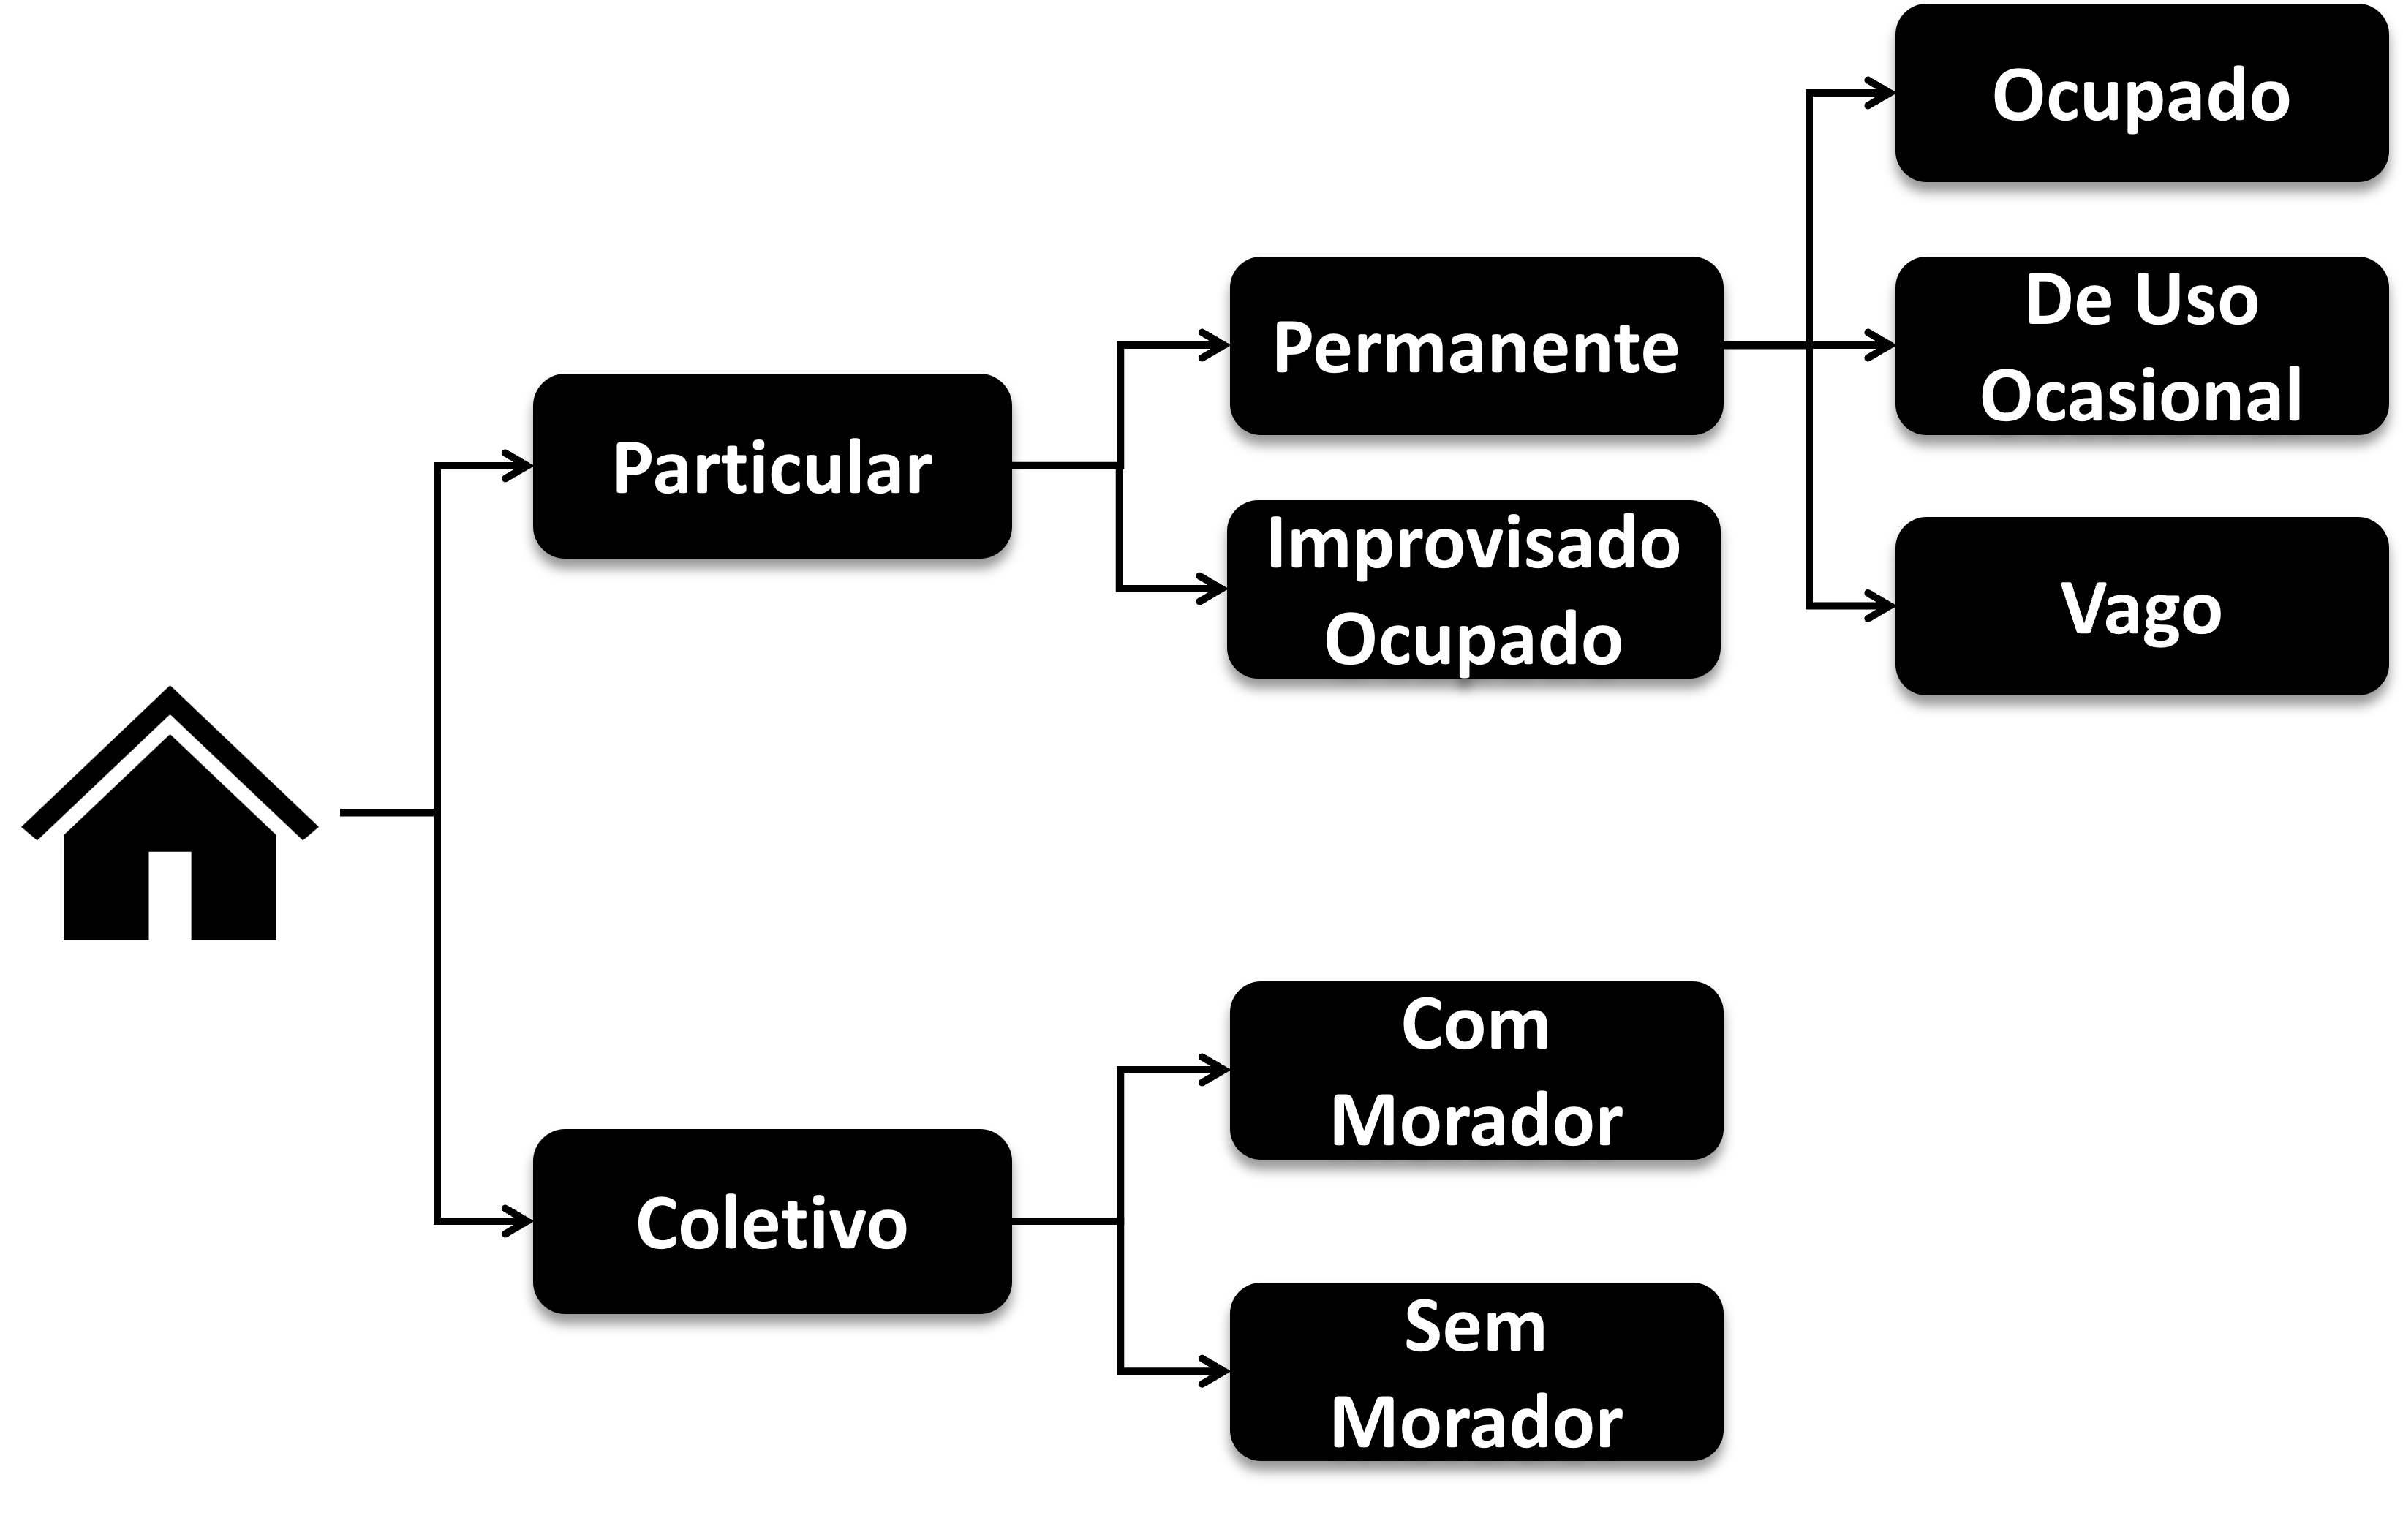
\includegraphics[keepaspectratio]{img/7-agregados/domicilios.png}}

}

\end{figure}%

A leitura da árvore começa pela distinção entre \textbf{particulares} e
\textbf{coletivos}. Os particulares são aqueles em que a convivência se
dá por laços de parentesco, dependência doméstica ou normas de
convivência, e se dividem entre os \textbf{permanentes}, construídos
para servir de moradia, e os \textbf{improvisados}, que ocupam
edificações ou espaços sem finalidade habitacional. Os permanentes, por
sua vez, admitem três situações na data de referência, com o domicílio
ocupado, vago ou de uso ocasional. Os coletivos são estabelecimentos
regidos por normas de subordinação administrativa, como quartéis,
presídios e asilos, e aparecem com ou sem morador.

Esses nomes são longos e reaparecem o tempo todo na documentação, razão
pela qual o IBGE trabalha com siglas. Elas estão reunidas na planilha
\texttt{Siglas\_Basico}, que é a primeira aba do dicionário aberto por
\texttt{data\_dictionary(year\ =\ 2022,\ dataset\ =\ "tracts")} e cujo
conteúdo a Tabela~\ref{tbl-hab-siglas} reproduz.

{

\begin{longtable}[]{@{}cl@{}}

\caption{\label{tbl-hab-siglas}Siglas dos tipos de domicílio do Censo
2022, conforme a planilha \texttt{Siglas\_Basico} do dicionário dos
Agregados por Setores Censitários.}

\tabularnewline

\toprule\noalign{}
Sigla & Descrição \\
\midrule\noalign{}
\endhead
\bottomrule\noalign{}
\endlastfoot
DPPO & Domicílio Particular Permanente Ocupado \\
DPIO & Domicílio Particular Improvisado Ocupado \\
DPPV & Domicílio Particular Permanente Vago \\
DPPUO & Domicílio Particular Permanente de Uso Ocasional \\
DCCM & Domicílio Coletivo Com Morador \\
DCSM & Domicílio Coletivo Sem Morador \\
DPO & Domicílio Particular Ocupado (DPPO + DPIO) \\

\end{longtable}

}

Note que a última linha já é uma soma. O DPO não é uma categoria da
árvore, e sim o agrupamento dos dois tipos de domicílio particular que
tinham morador na data de referência. Essa é a chave para entender o
restante, porque os totais de domicílio do arquivo Básico são definidos
no dicionário exatamente nesses termos, e não em linguagem corrente. A
Tabela~\ref{tbl-hab-somas} transcreve essas definições.

{

\begin{longtable}[]{@{}
  >{\centering\arraybackslash}p{(\linewidth - 4\tabcolsep) * \real{0.0926}}
  >{\raggedright\arraybackslash}p{(\linewidth - 4\tabcolsep) * \real{0.5278}}
  >{\raggedright\arraybackslash}p{(\linewidth - 4\tabcolsep) * \real{0.3796}}@{}}

\caption{\label{tbl-hab-somas}Composição dos totais de domicílio do
arquivo Básico dos Agregados por Setores Censitários, Censo 2022,
conforme o dicionário de dados.}

\tabularnewline

\toprule\noalign{}
\begin{minipage}[b]{\linewidth}\centering
Variável
\end{minipage} & \begin{minipage}[b]{\linewidth}\raggedright
Descrição
\end{minipage} & \begin{minipage}[b]{\linewidth}\raggedright
Composição
\end{minipage} \\
\midrule\noalign{}
\endhead
\bottomrule\noalign{}
\endlastfoot
\texttt{V0002} & Total de domicílios & DPPO + DPPV + DPPUO + DPIO + DCCM
+ DCSM \\
\texttt{V0003} & Total de domicílios particulares & DPPO + DPPV + DPPUO
+ DPIO \\
\texttt{V0004} & Total de domicílios coletivos & DCCM + DCSM \\
\texttt{V0005} & Média de moradores em domicílios particulares ocupados
& Pessoas em DPO / (DPPO + DPIO) \\
\texttt{V0006} & Percentual de domicílios particulares ocupados
imputados & DPO imputados / DPO \\
\texttt{V0007} & Total de domicílios particulares ocupados & DPPO +
DPIO \\

\end{longtable}

}

Duas consequências práticas saltam dessa tabela e valem ser fixadas
desde já. A primeira é que \texttt{V0003} não conta todos os domicílios
do setor, porque deixa os coletivos de fora, de modo que usá-lo como
denominador de um indicador que fale de ``domicílios'' em geral seria
incorreto. A segunda é que a diferença entre \texttt{V0003} e
\texttt{V0007} tem um significado preciso, já que subtrair DPPO + DPIO
de DPPO + DPPV + DPPUO + DPIO deixa como resto DPPV + DPPUO, ou seja, os
domicílios permanentes vagos somados aos de uso ocasional. Voltaremos a
essa subtração na Seção~\ref{sec-hab-nao-ocupados}, e ela explica por
que o indicador correspondente não pode ser chamado simplesmente de
vacância.

Vale lembrar que essas definições estão detalhadas na nota metodológica
dos Agregados por Setores Censitários (IBGE, 2024a), que é a referência
a consultar sempre que restar dúvida sobre o que um total específico
inclui. Com o vocabulário reposto, podemos organizar os dados do
capítulo.

\section{Estruturação dos dados de agregados do Censo de
2022}\label{sec-hab-dados}

Começamos pelos agregados, e tudo o que precisamos deles está no arquivo
\textbf{Básico}. De lá vêm a população, dois dos totais de domicílio da
Tabela~\ref{tbl-hab-somas} e a média de moradores, além do campo que
identifica os setores de Favela e Comunidade Urbana. A
Tabela~\ref{tbl-hab-variaveis} descreve o que será lido.

{

\begin{longtable}[]{@{}
  >{\centering\arraybackslash}p{(\linewidth - 6\tabcolsep) * \real{0.0804}}
  >{\centering\arraybackslash}p{(\linewidth - 6\tabcolsep) * \real{0.1518}}
  >{\centering\arraybackslash}p{(\linewidth - 6\tabcolsep) * \real{0.1429}}
  >{\raggedright\arraybackslash}p{(\linewidth - 6\tabcolsep) * \real{0.6250}}@{}}

\caption{\label{tbl-hab-variaveis}Variáveis dos Agregados por Setor
Censitário utilizadas neste capítulo (Censo 2022).}

\tabularnewline

\toprule\noalign{}
\begin{minipage}[b]{\linewidth}\centering
Arquivo
\end{minipage} & \begin{minipage}[b]{\linewidth}\centering
Código original
\end{minipage} & \begin{minipage}[b]{\linewidth}\centering
Nome atribuído
\end{minipage} & \begin{minipage}[b]{\linewidth}\raggedright
Descrição
\end{minipage} \\
\midrule\noalign{}
\endhead
\bottomrule\noalign{}
\endlastfoot
Básico & \texttt{V0001} & \texttt{pop} & População total residente \\
Básico & \texttt{V0003} & \texttt{dom\_part} & Total de domicílios
particulares (ocupados, vagos e de uso ocasional) \\
Básico & \texttt{V0005} & \texttt{mor\_dom} & Média de moradores em
domicílios particulares ocupados \\
Básico & \texttt{V0007} & \texttt{dom\_ocup} & Total de domicílios
particulares ocupados \\
Básico & \texttt{code\_type} & --- & Tipo do setor, em que 1 indica
Favela e Comunidade Urbana \\

\end{longtable}

}

Obtemos primeiro o código do município e, em seguida, lemos os dois
arquivos, filtrando por João Pessoa antes do \texttt{collect()}.

\begin{Shaded}
\begin{Highlighting}[]
\NormalTok{joao\_pessoa }\OtherTok{\textless{}{-}} \FunctionTok{lookup\_muni}\NormalTok{(}\AttributeTok{name\_muni =} \StringTok{"João Pessoa"}\NormalTok{, }\AttributeTok{year =} \DecValTok{2022}\NormalTok{)}\SpecialCharTok{$}\NormalTok{code\_muni}
\NormalTok{joao\_pessoa}
\end{Highlighting}
\end{Shaded}

\begin{verbatim}
[1] 2507507
\end{verbatim}

Do arquivo Básico pedimos também \texttt{name\_neighborhood} e
\texttt{code\_type}, que serão usados adiante para agregar os resultados
e para separar os setores classificados como Favela e Comunidade Urbana.

\begin{Shaded}
\begin{Highlighting}[]
\NormalTok{jp\_sc }\OtherTok{\textless{}{-}} \FunctionTok{read\_tracts}\NormalTok{(}\AttributeTok{dataset =} \StringTok{"Basico"}\NormalTok{, }\AttributeTok{year =} \DecValTok{2022}\NormalTok{) }\SpecialCharTok{|\textgreater{}}
  \FunctionTok{filter}\NormalTok{(code\_muni }\SpecialCharTok{==}\NormalTok{ joao\_pessoa) }\SpecialCharTok{|\textgreater{}}
  \FunctionTok{select}\NormalTok{(code\_tract, name\_neighborhood, code\_type, V0001, V0003, V0005, V0007) }\SpecialCharTok{|\textgreater{}}
  \FunctionTok{collect}\NormalTok{() }\SpecialCharTok{|\textgreater{}}
  \FunctionTok{rename}\NormalTok{(}
    \AttributeTok{pop      =}\NormalTok{ V0001,}
    \AttributeTok{dom\_part =}\NormalTok{ V0003,}
    \AttributeTok{mor\_dom  =}\NormalTok{ V0005,}
    \AttributeTok{dom\_ocup =}\NormalTok{ V0007}
\NormalTok{  )}

\FunctionTok{nrow}\NormalTok{(jp\_sc)}
\end{Highlighting}
\end{Shaded}

\begin{verbatim}
[1] 1778
\end{verbatim}

Precisamos ainda da geometria dos setores, que virá do \texttt{geobr} e
será unida à tabela pela coluna \texttt{code\_tract}.

\begin{Shaded}
\begin{Highlighting}[]
\NormalTok{jp\_geo }\OtherTok{\textless{}{-}} \FunctionTok{read\_census\_tract}\NormalTok{(}
  \AttributeTok{code\_tract =}\NormalTok{ joao\_pessoa,}
  \AttributeTok{year       =} \DecValTok{2022}\NormalTok{,}
  \AttributeTok{simplified =} \ConstantTok{FALSE}
\NormalTok{) }\SpecialCharTok{|\textgreater{}}
  \FunctionTok{select}\NormalTok{(code\_tract) }\SpecialCharTok{|\textgreater{}}
  \FunctionTok{left\_join}\NormalTok{(jp\_sc, }\AttributeTok{by =} \StringTok{"code\_tract"}\NormalTok{)}
\end{Highlighting}
\end{Shaded}

Antes de calcular qualquer coisa, uma verificação de coerência. Os três
totais de domicílios do arquivo Básico têm de guardar entre si a relação
que suas definições anunciam, com o total de particulares maior que o de
particulares ocupados.

\begin{Shaded}
\begin{Highlighting}[]
\NormalTok{jp\_sc }\SpecialCharTok{|\textgreater{}}
  \FunctionTok{summarize}\NormalTok{(}
    \AttributeTok{populacao      =} \FunctionTok{sum}\NormalTok{(pop,      }\AttributeTok{na.rm =} \ConstantTok{TRUE}\NormalTok{),}
    \AttributeTok{dom\_particular =} \FunctionTok{sum}\NormalTok{(dom\_part, }\AttributeTok{na.rm =} \ConstantTok{TRUE}\NormalTok{),}
    \AttributeTok{dom\_ocupado    =} \FunctionTok{sum}\NormalTok{(dom\_ocup, }\AttributeTok{na.rm =} \ConstantTok{TRUE}\NormalTok{),}
    \AttributeTok{diferenca      =} \FunctionTok{sum}\NormalTok{(dom\_part, }\AttributeTok{na.rm =} \ConstantTok{TRUE}\NormalTok{) }\SpecialCharTok{{-}} \FunctionTok{sum}\NormalTok{(dom\_ocup, }\AttributeTok{na.rm =} \ConstantTok{TRUE}\NormalTok{)}
\NormalTok{  )}
\end{Highlighting}
\end{Shaded}

\begin{verbatim}
  populacao dom_particular dom_ocupado diferenca
1    833932         377504      296743     80761
\end{verbatim}

A diferença entre os dois totais passa de oitenta mil domicílios, e a
Tabela~\ref{tbl-hab-somas} já nos diz o que ela contém. É desse resto
que trata a próxima seção.

\section{Domicílios particulares não
ocupados}\label{sec-hab-nao-ocupados}

Nenhuma variável dos Agregados de 2022 informa diretamente quantos
domicílios estão vagos. O que existe são os dois totais que já lemos, e
a diferença entre eles.

\[
\text{não ocupados} = \underbrace{V0003}_{\text{particulares}} - \underbrace{V0007}_{\text{particulares ocupados}}
\]

Pela composição vista na Seção~\ref{sec-hab-tipos}, o resto dessa
subtração é \textbf{DPPV + DPPUO}, e é por isso que ele não pode ser
lido estritamente como total de vagos. As duas categorias descrevem
situações bem diferentes, porque um imóvel vago está fora de uso e um
imóvel de uso ocasional é a casa de praia que fica fechada durante boa
parte do ano, por exemplo.

Há, porém, um sentido em que somar as duas é exatamente o que interessa.
Quando a pergunta é quanto do estoque construído está servindo de
moradia regular, o que importa é a ocupação habitual e, a rigor, nem o
domicílio vago nem o de uso ocasional a cumprem. Por esse ângulo, os
dois são estoque edificado que existe e não abriga ninguém de forma
permanente, o que faz da soma uma medida abrangente do uso do parque
residencial, útil para uma análise voltada a políticas de habitação.
Deste modo, a impossibilidade de separá-las nos agregados deixa de ser
apenas uma limitação da fonte e passa a coincidir com o que se quer
medir.

Isso não dispensa o cuidado com o nome. O vazio de mercado e a segunda
residência têm causas distintas e pedem respostas distintas, de modo que
o indicador precisa ser apresentado pelo que ele de fato mede, sem ser
convertido em taxa de vacância. Partindo para o seu cômputo, temos
então:

\begin{Shaded}
\begin{Highlighting}[]
\NormalTok{jp\_geo }\OtherTok{\textless{}{-}}\NormalTok{ jp\_geo }\SpecialCharTok{|\textgreater{}}
  \FunctionTok{mutate}\NormalTok{(}
    \AttributeTok{nao\_ocup      =}\NormalTok{ dom\_part }\SpecialCharTok{{-}}\NormalTok{ dom\_ocup,}
    \AttributeTok{perc\_nao\_ocup =} \DecValTok{100} \SpecialCharTok{*}\NormalTok{ nao\_ocup }\SpecialCharTok{/}\NormalTok{ dom\_part}
\NormalTok{  )}

\NormalTok{jp\_geo }\SpecialCharTok{|\textgreater{}}
  \FunctionTok{st\_drop\_geometry}\NormalTok{() }\SpecialCharTok{|\textgreater{}}
  \FunctionTok{summarize}\NormalTok{(}
    \AttributeTok{nao\_ocupados =} \FunctionTok{sum}\NormalTok{(nao\_ocup, }\AttributeTok{na.rm =} \ConstantTok{TRUE}\NormalTok{),}
    \AttributeTok{percentual   =} \DecValTok{100} \SpecialCharTok{*} \FunctionTok{sum}\NormalTok{(nao\_ocup, }\AttributeTok{na.rm =} \ConstantTok{TRUE}\NormalTok{) }\SpecialCharTok{/} \FunctionTok{sum}\NormalTok{(dom\_part, }\AttributeTok{na.rm =} \ConstantTok{TRUE}\NormalTok{)}
\NormalTok{  )}
\end{Highlighting}
\end{Shaded}

\begin{verbatim}
# A tibble: 1 x 2
  nao_ocupados percentual
         <dbl>      <dbl>
1        80761       21.4
\end{verbatim}

Note que mais de um em cada cinco domicílios particulares de João Pessoa
não tinha morador (ou morador regular) em 2022. É uma proporção alta, e
o mapa mostra que ela está longe de se distribuir por igual:

\begin{Shaded}
\begin{Highlighting}[]
\FunctionTok{ggplot}\NormalTok{(jp\_geo) }\SpecialCharTok{+}
  \FunctionTok{geom\_sf}\NormalTok{(}\FunctionTok{aes}\NormalTok{(}\AttributeTok{fill =}\NormalTok{ perc\_nao\_ocup), }\AttributeTok{color =} \ConstantTok{NA}\NormalTok{) }\SpecialCharTok{+}
  \FunctionTok{scale\_fill\_distiller}\NormalTok{(}\AttributeTok{palette =} \StringTok{"OrRd"}\NormalTok{, }\AttributeTok{direction =} \DecValTok{1}\NormalTok{,}
                       \AttributeTok{name =} \StringTok{"\% não}\SpecialCharTok{\textbackslash{}n}\StringTok{ocupados"}\NormalTok{,}
                       \AttributeTok{na.value =} \StringTok{"gray90"}\NormalTok{) }\SpecialCharTok{+}
  \FunctionTok{coord\_sf}\NormalTok{(}\AttributeTok{expand =} \ConstantTok{FALSE}\NormalTok{) }\SpecialCharTok{+}
  \FunctionTok{theme\_minimal}\NormalTok{() }\SpecialCharTok{+}
  \FunctionTok{theme}\NormalTok{(}\AttributeTok{axis.text =} \FunctionTok{element\_blank}\NormalTok{(), }\AttributeTok{axis.ticks =} \FunctionTok{element\_blank}\NormalTok{(),}
        \AttributeTok{panel.grid =} \FunctionTok{element\_blank}\NormalTok{())}
\end{Highlighting}
\end{Shaded}

\begin{figure}[H]

\caption{\label{fig-nao-ocupados}Proporção de domicílios particulares
não ocupados, somando vagos e de uso ocasional, por setor censitário,
João Pessoa (PB), Censo 2022.}

\centering{

\pandocbounded{
\includegraphics[keepaspectratio]{13-habitacao_files/figure-pdf/fig-nao-ocupados-1.pdf}}

}

\end{figure}%

Para nomear as áreas, agregamos por bairro. Aqui cabe uma observação
prática que continua a do Capítulo 12. Em Goiânia, a coluna
\texttt{name\_neighborhood} vinha inteiramente vazia e tivemos de
recorrer ao subdistrito. Em João Pessoa acontece o contrário, com os
bairros preenchidos e o município inteiro formando um único distrito e
um único subdistrito. Não existe um recorte intermediário que sirva para
todos os municípios, e a verificação precisa ser feita caso a caso.

\begin{Shaded}
\begin{Highlighting}[]
\NormalTok{jp\_sc }\SpecialCharTok{|\textgreater{}}
  \FunctionTok{summarize}\NormalTok{(}
    \AttributeTok{bairros\_distintos =} \FunctionTok{n\_distinct}\NormalTok{(name\_neighborhood),}
    \AttributeTok{setores\_sem\_bairro =} \FunctionTok{sum}\NormalTok{(}\FunctionTok{is.na}\NormalTok{(name\_neighborhood))}
\NormalTok{  )}
\end{Highlighting}
\end{Shaded}

\begin{verbatim}
  bairros_distintos setores_sem_bairro
1                65                 14
\end{verbatim}

Com 65 bairros preenchidos, a agregação é viável. Restringimos a tabela
aos bairros com pelo menos mil domicílios particulares, para que
proporções calculadas sobre bases muito pequenas não dominem os
extremos.

\begin{Shaded}
\begin{Highlighting}[]
\NormalTok{bairros }\OtherTok{\textless{}{-}}\NormalTok{ jp\_geo }\SpecialCharTok{|\textgreater{}}
  \FunctionTok{st\_drop\_geometry}\NormalTok{() }\SpecialCharTok{|\textgreater{}}
  \FunctionTok{filter}\NormalTok{(}\SpecialCharTok{!}\FunctionTok{is.na}\NormalTok{(name\_neighborhood)) }\SpecialCharTok{|\textgreater{}}
  \FunctionTok{group\_by}\NormalTok{(name\_neighborhood) }\SpecialCharTok{|\textgreater{}}
  \FunctionTok{summarize}\NormalTok{(}
    \AttributeTok{pop      =} \FunctionTok{sum}\NormalTok{(pop,      }\AttributeTok{na.rm =} \ConstantTok{TRUE}\NormalTok{),}
    \AttributeTok{dom\_part =} \FunctionTok{sum}\NormalTok{(dom\_part, }\AttributeTok{na.rm =} \ConstantTok{TRUE}\NormalTok{),}
    \AttributeTok{dom\_ocup =} \FunctionTok{sum}\NormalTok{(dom\_ocup, }\AttributeTok{na.rm =} \ConstantTok{TRUE}\NormalTok{)}
\NormalTok{  ) }\SpecialCharTok{|\textgreater{}}
  \FunctionTok{filter}\NormalTok{(dom\_part }\SpecialCharTok{\textgreater{}=} \DecValTok{1000}\NormalTok{) }\SpecialCharTok{|\textgreater{}}
  \FunctionTok{mutate}\NormalTok{(}\AttributeTok{perc\_nao\_ocup =} \DecValTok{100} \SpecialCharTok{*}\NormalTok{ (dom\_part }\SpecialCharTok{{-}}\NormalTok{ dom\_ocup) }\SpecialCharTok{/}\NormalTok{ dom\_part)}

\FunctionTok{bind\_rows}\NormalTok{(}
\NormalTok{  bairros }\SpecialCharTok{|\textgreater{}} \FunctionTok{slice\_max}\NormalTok{(perc\_nao\_ocup, }\AttributeTok{n =} \DecValTok{8}\NormalTok{),}
\NormalTok{  bairros }\SpecialCharTok{|\textgreater{}} \FunctionTok{slice\_min}\NormalTok{(perc\_nao\_ocup, }\AttributeTok{n =} \DecValTok{5}\NormalTok{)}
\NormalTok{) }\SpecialCharTok{|\textgreater{}}
  \FunctionTok{select}\NormalTok{(name\_neighborhood, dom\_part, perc\_nao\_ocup) }\SpecialCharTok{|\textgreater{}}
\NormalTok{  knitr}\SpecialCharTok{::}\FunctionTok{kable}\NormalTok{(}
    \AttributeTok{col.names =} \FunctionTok{c}\NormalTok{(}\StringTok{"Bairro"}\NormalTok{, }\StringTok{"Domicílios particulares"}\NormalTok{, }\StringTok{"\% não ocupados"}\NormalTok{),}
    \AttributeTok{digits =} \DecValTok{1}\NormalTok{,}
    \AttributeTok{format.args =} \FunctionTok{list}\NormalTok{(}\AttributeTok{big.mark =} \StringTok{"."}\NormalTok{, }\AttributeTok{decimal.mark =} \StringTok{","}\NormalTok{)}
\NormalTok{  )}
\end{Highlighting}
\end{Shaded}

{

\begin{longtable}[]{@{}lrr@{}}

\caption{\label{tbl-hab-nao-ocup-bairro}Bairros de João Pessoa (PB) com
as maiores e as menores proporções de domicílios particulares não
ocupados, entre os que possuem ao menos mil domicílios particulares,
Censo 2022.}

\tabularnewline

\toprule\noalign{}
Bairro & Domicílios particulares & \% não ocupados \\
\midrule\noalign{}
\endhead
\bottomrule\noalign{}
\endlastfoot
Cabo Branco & 6.831 & 48,7 \\
Varadouro & 1.546 & 40,7 \\
Tambaú & 6.280 & 35,5 \\
Muçumagro & 6.859 & 32,5 \\
Centro & 1.483 & 32,4 \\
Bessa & 9.386 & 31,1 \\
Água Fria & 4.011 & 30,9 \\
Jardim Oceania & 11.154 & 27,1 \\
São José & 2.399 & 12,1 \\
Treze de Maio & 3.129 & 12,6 \\
Padre Zé & 2.354 & 14,1 \\
Alto do Céu & 7.554 & 14,4 \\
Costa e Silva & 2.676 & 14,5 \\

\end{longtable}

}

A tabela revela dois fenômenos distintos misturados no mesmo indicador,
e é justamente por isso que ele não pode ser chamado de vacância. No
topo aparecem bairros da orla, onde a proporção de domicílios sem
morador chega a quase metade do estoque, padrão compatível com segunda
residência e uso de veraneio. Também no topo aparecem o Centro e o
Varadouro, que ficam do lado oposto da cidade e cuja história é outra, a
de esvaziamento de área central consolidada. Somar os dois casos em um
único número é aceitável desde que a leitura os separe.

A tabela nomeia os extremos, mas não diz onde eles estão. Para isso
precisamos da malha de bairros, que o \texttt{geobr} fornece pela função
\texttt{read\_neighborhood()}, e de uma junção com os valores já
calculados. O mapa da Figura~\ref{fig-hab-bairros} repete a escala de
cores usada por setor censitário, agora com o bairro como unidade, e
rotula os oito de maior proporção com a geometria
\texttt{geom\_sf\_label()}.

\begin{Shaded}
\begin{Highlighting}[]
\NormalTok{bairros\_geo }\OtherTok{\textless{}{-}} \FunctionTok{read\_neighborhood}\NormalTok{(}\AttributeTok{year =} \DecValTok{2022}\NormalTok{, }\AttributeTok{code\_muni =}\NormalTok{ joao\_pessoa)}

\NormalTok{bairros\_mapa }\OtherTok{\textless{}{-}}\NormalTok{ bairros\_geo }\SpecialCharTok{|\textgreater{}}
  \FunctionTok{select}\NormalTok{(name\_neighborhood) }\SpecialCharTok{|\textgreater{}}
  \FunctionTok{left\_join}\NormalTok{(bairros, }\AttributeTok{by =} \StringTok{"name\_neighborhood"}\NormalTok{)}

\NormalTok{destaques }\OtherTok{\textless{}{-}}\NormalTok{ bairros\_mapa }\SpecialCharTok{|\textgreater{}}
  \FunctionTok{slice\_max}\NormalTok{(perc\_nao\_ocup, }\AttributeTok{n =} \DecValTok{8}\NormalTok{)}

\FunctionTok{ggplot}\NormalTok{(bairros\_mapa) }\SpecialCharTok{+}
  \FunctionTok{geom\_sf}\NormalTok{(}\FunctionTok{aes}\NormalTok{(}\AttributeTok{fill =}\NormalTok{ perc\_nao\_ocup), }\AttributeTok{color =} \StringTok{"white"}\NormalTok{, }\AttributeTok{linewidth =} \FloatTok{0.2}\NormalTok{) }\SpecialCharTok{+}
  \FunctionTok{geom\_sf\_label}\NormalTok{(}\AttributeTok{data =}\NormalTok{ destaques, }\FunctionTok{aes}\NormalTok{(}\AttributeTok{label =}\NormalTok{ name\_neighborhood),}
                \AttributeTok{size =} \FloatTok{2.2}\NormalTok{, }\AttributeTok{alpha =} \FloatTok{0.85}\NormalTok{,}
                \AttributeTok{label.padding =} \FunctionTok{unit}\NormalTok{(}\FloatTok{0.12}\NormalTok{, }\StringTok{"lines"}\NormalTok{)) }\SpecialCharTok{+}
  \FunctionTok{scale\_fill\_distiller}\NormalTok{(}\AttributeTok{palette =} \StringTok{"OrRd"}\NormalTok{, }\AttributeTok{direction =} \DecValTok{1}\NormalTok{,}
                       \AttributeTok{name =} \StringTok{"\% não}\SpecialCharTok{\textbackslash{}n}\StringTok{ocupados"}\NormalTok{,}
                       \AttributeTok{na.value =} \StringTok{"gray90"}\NormalTok{) }\SpecialCharTok{+}
  \FunctionTok{coord\_sf}\NormalTok{(}\AttributeTok{expand =} \ConstantTok{FALSE}\NormalTok{) }\SpecialCharTok{+}
  \FunctionTok{labs}\NormalTok{(}\AttributeTok{x =} \ConstantTok{NULL}\NormalTok{, }\AttributeTok{y =} \ConstantTok{NULL}\NormalTok{) }\SpecialCharTok{+}
  \FunctionTok{theme\_minimal}\NormalTok{() }\SpecialCharTok{+}
  \FunctionTok{theme}\NormalTok{(}\AttributeTok{axis.text =} \FunctionTok{element\_blank}\NormalTok{(), }\AttributeTok{axis.ticks =} \FunctionTok{element\_blank}\NormalTok{(),}
        \AttributeTok{panel.grid =} \FunctionTok{element\_blank}\NormalTok{())}
\end{Highlighting}
\end{Shaded}

\begin{figure}[H]

\caption{\label{fig-hab-bairros}Proporção de domicílios particulares não
ocupados por bairro, com destaque para os oito de maior proporção, João
Pessoa (PB), Censo 2022.}

\centering{

\pandocbounded{
\includegraphics[keepaspectratio]{13-habitacao_files/figure-pdf/fig-hab-bairros-1.pdf}}

}

\end{figure}%

O mapa mostra que os oito bairros do topo não formam um grupo homogêneo.
Quatro deles, Cabo Branco, Tambaú, Bessa e Jardim Oceania, estão numa
faixa contínua junto ao litoral, o que sustenta a hipótese da segunda
residência. O Centro e o Varadouro são vizinhos entre si e ficam
afastados do mar, correspondendo ao padrão de área central esvaziada.
Sobram Muçumagro e Água Fria, no interior do município, que não se
encaixam em nenhum dos dois padrões e lembram que o indicador reúne
situações mais variadas do que a leitura pela orla e pelo centro faz
supor.

Resta uma última comparação, levando em consideração a característica do
setor ser de favela/comunidade urbana ou não. Conforme descrito
anteriormente, em caso afirmativo a coluna \texttt{code\_type} recebe
valor 1. Contrastando esses tipos de setor com os demais, temos então:

\begin{Shaded}
\begin{Highlighting}[]
\NormalTok{jp\_geo }\SpecialCharTok{|\textgreater{}}
  \FunctionTok{st\_drop\_geometry}\NormalTok{() }\SpecialCharTok{|\textgreater{}}
  \FunctionTok{mutate}\NormalTok{(}
    \AttributeTok{tipo =} \FunctionTok{ifelse}\NormalTok{(code\_type }\SpecialCharTok{==} \DecValTok{1}\NormalTok{, }\StringTok{"Favela e Comunidade Urbana"}\NormalTok{, }\StringTok{"Demais setores"}\NormalTok{)}
\NormalTok{  ) }\SpecialCharTok{|\textgreater{}}
  \FunctionTok{group\_by}\NormalTok{(tipo) }\SpecialCharTok{|\textgreater{}}
  \FunctionTok{summarize}\NormalTok{(}
    \AttributeTok{dom\_part =} \FunctionTok{sum}\NormalTok{(dom\_part, }\AttributeTok{na.rm =} \ConstantTok{TRUE}\NormalTok{),}
    \AttributeTok{dom\_ocup =} \FunctionTok{sum}\NormalTok{(dom\_ocup, }\AttributeTok{na.rm =} \ConstantTok{TRUE}\NormalTok{)}
\NormalTok{  ) }\SpecialCharTok{|\textgreater{}}
  \FunctionTok{mutate}\NormalTok{(}\AttributeTok{perc\_nao\_ocup =} \DecValTok{100} \SpecialCharTok{*}\NormalTok{ (dom\_part }\SpecialCharTok{{-}}\NormalTok{ dom\_ocup) }\SpecialCharTok{/}\NormalTok{ dom\_part) }\SpecialCharTok{|\textgreater{}}
\NormalTok{  knitr}\SpecialCharTok{::}\FunctionTok{kable}\NormalTok{(}
    \AttributeTok{digits =} \DecValTok{1}\NormalTok{,}
    \AttributeTok{format.args =} \FunctionTok{list}\NormalTok{(}\AttributeTok{big.mark =} \StringTok{"."}\NormalTok{, }\AttributeTok{decimal.mark =} \StringTok{","}\NormalTok{)}
\NormalTok{  )}
\end{Highlighting}
\end{Shaded}

{

\begin{longtable}[]{@{}lrrr@{}}

\caption{\label{tbl-hab-nao-ocup-favela}Domicílios particulares não
ocupados em João Pessoa (PB), comparando os setores de Favela e
Comunidade Urbana aos demais setores, Censo 2022.}

\tabularnewline

\toprule\noalign{}
tipo & dom\_part & dom\_ocup & perc\_nao\_ocup \\
\midrule\noalign{}
\endhead
\bottomrule\noalign{}
\endlastfoot
Demais setores & 331.369 & 258.694 & 21,9 \\
Favela e Comunidade Urbana & 46.135 & 38.049 & 17,5 \\

\end{longtable}

}

Observe que a proporção de domicílios sem morador é ligeiramente menor
dentro das favelas e comunidades urbanas do que no restante da cidade,
resultado coerente com o que o indicador mede. Domicílio de uso
ocasional pressupõe que alguém disponha de uma segunda casa, e domicílio
vago pressupõe estoque à espera de comprador ou inquilino (ou mera
especulação). Onde a moradia é escassa e disputada, o espaço construído
tende a ser ocupado para morar, qualquer que seja sua qualidade, e sobra
pouco imóvel fora de uso. O estoque sem morador se concentra em outras
situações, como a orla de segunda residência e a área central que perdeu
população para as frentes de expansão, que foi o que a
Figura~\ref{fig-hab-bairros} mostrou.

Contamos até aqui quantos domicílios existem e quantos estão vazios.
Falta a pergunta oposta, que é quantas pessoas ocupam os que estão
cheios.

\section{Quantas pessoas por domicílio}\label{sec-hab-moradores}

O arquivo Básico traz a variável \texttt{V0005}, que é a média de
moradores em domicílios particulares ocupados de cada setor. Ela merece
um cuidado que as demais variáveis dos agregados não exigem, porque
\textbf{já chega calculada como média}. Não se relativiza uma média, não
se soma média de setores diferentes e, ao agregar para bairro, é preciso
reconstruir o quociente a partir dos totais, e não tirar a média das
médias.

Comecemos observando a distribuição da variável entre os setores do
município.

\begin{Shaded}
\begin{Highlighting}[]
\FunctionTok{summary}\NormalTok{(jp\_geo}\SpecialCharTok{$}\NormalTok{mor\_dom)}
\end{Highlighting}
\end{Shaded}

\begin{verbatim}
   Min. 1st Qu.  Median    Mean 3rd Qu.    Max. 
   0.00    2.60    2.80    2.75    3.00    6.50 
\end{verbatim}

Os quartis estão muito próximos uns dos outros, o que sugere pouca
variação entre setores. O mapa confirma essa impressão.

\begin{Shaded}
\begin{Highlighting}[]
\FunctionTok{ggplot}\NormalTok{(jp\_geo) }\SpecialCharTok{+}
  \FunctionTok{geom\_sf}\NormalTok{(}\FunctionTok{aes}\NormalTok{(}\AttributeTok{fill =}\NormalTok{ mor\_dom), }\AttributeTok{color =} \ConstantTok{NA}\NormalTok{) }\SpecialCharTok{+}
  \FunctionTok{scale\_fill\_distiller}\NormalTok{(}\AttributeTok{palette =} \StringTok{"Purples"}\NormalTok{, }\AttributeTok{direction =} \DecValTok{1}\NormalTok{,}
                       \AttributeTok{name =} \StringTok{"Moradores por}\SpecialCharTok{\textbackslash{}n}\StringTok{domicílio"}\NormalTok{,}
                       \AttributeTok{na.value =} \StringTok{"gray90"}\NormalTok{) }\SpecialCharTok{+}
  \FunctionTok{coord\_sf}\NormalTok{(}\AttributeTok{expand =} \ConstantTok{FALSE}\NormalTok{) }\SpecialCharTok{+}
  \FunctionTok{theme\_minimal}\NormalTok{() }\SpecialCharTok{+}
  \FunctionTok{theme}\NormalTok{(}\AttributeTok{axis.text =} \FunctionTok{element\_blank}\NormalTok{(), }\AttributeTok{axis.ticks =} \FunctionTok{element\_blank}\NormalTok{(),}
        \AttributeTok{panel.grid =} \FunctionTok{element\_blank}\NormalTok{())}
\end{Highlighting}
\end{Shaded}

\begin{figure}[H]

\caption{\label{fig-moradores}Média de moradores em domicílios
particulares ocupados, por setor censitário, João Pessoa (PB), Censo
2022.}

\centering{

\pandocbounded{
\includegraphics[keepaspectratio]{13-habitacao_files/figure-pdf/fig-moradores-1.pdf}}

}

\end{figure}%

A variação entre setores é modesta, com a maior parte da cidade entre
dois e meio e três moradores por domicílio. Essa compressão é esperada,
porque o tamanho médio das famílias brasileiras caiu muito e ficou
parecido entre classes de renda. É também a razão pela qual esse
indicador, sozinho, diz pouco sobre adensamento.

O motivo é simples. Três pessoas em um domicílio de três dormitórios e
três pessoas em um domicílio de um dormitório produzem exatamente a
mesma média de moradores, e são situações habitacionais completamente
diferentes. O que distingue as duas é o número de dormitórios, e essa
informação não existe nos agregados.

\section{Quantas pessoas por dormitório}\label{sec-hab-dormitorio}

O quesito sobre cômodos usados como dormitório pertence ao Questionário
da Amostra, e por isso a resposta está nos microdados. O Censo 2010
divulga inclusive a razão já calculada, na variável \texttt{V6204}, que
é a densidade de moradores por dormitório do domicílio.

Como no Capítulo 12, a mudança de fonte traz mudança de unidade espacial
e de ano. Os microdados de 2022 ainda não foram divulgados, conforme
discutido no Capítulo 8, de modo que trabalhamos com 2010. Comecemos
verificando a quantidade de áreas de ponderação para João Pessoa:

\begin{Shaded}
\begin{Highlighting}[]
\NormalTok{ap\_jp }\OtherTok{\textless{}{-}} \FunctionTok{read\_weighting\_area}\NormalTok{(}
  \AttributeTok{code\_weighting =}\NormalTok{ joao\_pessoa,}
  \AttributeTok{year           =} \DecValTok{2010}\NormalTok{,}
  \AttributeTok{simplified     =} \ConstantTok{FALSE}
\NormalTok{)}

\NormalTok{ap\_cods }\OtherTok{\textless{}{-}}\NormalTok{ ap\_jp }\SpecialCharTok{|\textgreater{}}
  \FunctionTok{pull}\NormalTok{(code\_weighting)}

\FunctionTok{length}\NormalTok{(ap\_cods)}
\end{Highlighting}
\end{Shaded}

\begin{verbatim}
[1] 12
\end{verbatim}

São apenas doze áreas de ponderação para todo o município, contra os
1.778 setores censitários usados nas seções anteriores. Guardemos esse
contraste, porque ele é o assunto da seção seguinte.

A leitura dos microdados de domicílios segue o fluxo do Capítulo 8. Além
da variável de interesse, pedimos o identificador do domicílio, o peso
amostral e a área de ponderação, exigidos pelo plano amostral.

\begin{Shaded}
\begin{Highlighting}[]
\NormalTok{cols\_dom }\OtherTok{\textless{}{-}} \FunctionTok{c}\NormalTok{(}
  \StringTok{"V0300"}\NormalTok{,          }\CommentTok{\# Identificador do domicílio}
  \StringTok{"V0010"}\NormalTok{,          }\CommentTok{\# Peso amostral calibrado}
  \StringTok{"code\_weighting"}\NormalTok{, }\CommentTok{\# Área de ponderação}
  \StringTok{"V0204"}\NormalTok{,          }\CommentTok{\# Número de cômodos servindo de dormitório}
  \StringTok{"V6204"}           \CommentTok{\# Densidade de moradores por dormitório}
\NormalTok{)}

\NormalTok{md\_jp }\OtherTok{\textless{}{-}} \FunctionTok{read\_households}\NormalTok{(}\AttributeTok{year =} \DecValTok{2010}\NormalTok{, }\AttributeTok{columns =}\NormalTok{ cols\_dom) }\SpecialCharTok{|\textgreater{}}
  \FunctionTok{filter}\NormalTok{(code\_weighting }\SpecialCharTok{\%in\%}\NormalTok{ ap\_cods) }\SpecialCharTok{|\textgreater{}}
  \FunctionTok{collect}\NormalTok{()}

\FunctionTok{nrow}\NormalTok{(md\_jp)}
\end{Highlighting}
\end{Shaded}

\begin{verbatim}
[1] 10677
\end{verbatim}

Lembre-se que, no caso dos domicílios, o plano amostral é uma amostragem
estratificada, sem conglomeração, porque o domicílio é a própria unidade
sorteada. Declaramos, então, os estratos, os pesos e o total expandido
por área para a correção de população finita:

\begin{Shaded}
\begin{Highlighting}[]
\NormalTok{dom\_ap }\OtherTok{\textless{}{-}}\NormalTok{ md\_jp }\SpecialCharTok{|\textgreater{}}
  \FunctionTok{group\_by}\NormalTok{(code\_weighting) }\SpecialCharTok{|\textgreater{}}
  \FunctionTok{summarize}\NormalTok{(}\AttributeTok{n\_dom =} \FunctionTok{sum}\NormalTok{(V0010))}

\NormalTok{md\_jp }\OtherTok{\textless{}{-}}\NormalTok{ md\_jp }\SpecialCharTok{|\textgreater{}}
  \FunctionTok{left\_join}\NormalTok{(dom\_ap, }\AttributeTok{by =} \FunctionTok{join\_by}\NormalTok{(code\_weighting))}

\NormalTok{pa\_jp }\OtherTok{\textless{}{-}}\NormalTok{ md\_jp }\SpecialCharTok{|\textgreater{}}
  \FunctionTok{as\_survey\_design}\NormalTok{(}
    \AttributeTok{strata  =}\NormalTok{ code\_weighting,}
    \AttributeTok{weights =}\NormalTok{ V0010,}
    \AttributeTok{fpc     =}\NormalTok{ n\_dom}
\NormalTok{  )}
\end{Highlighting}
\end{Shaded}

Um detalhe preliminar importante é que precisamos olhar os valores
ausentes, porque neste caso eles não vêm de sigilo e sim de uma
característica real do domicílio:

\begin{Shaded}
\begin{Highlighting}[]
\NormalTok{md\_jp }\SpecialCharTok{|\textgreater{}}
  \FunctionTok{summarize}\NormalTok{(}
    \AttributeTok{registros        =} \FunctionTok{n}\NormalTok{(),}
    \AttributeTok{sem\_dormitorio   =} \FunctionTok{sum}\NormalTok{(}\FunctionTok{is.na}\NormalTok{(V0204)),}
    \AttributeTok{sem\_densidade    =} \FunctionTok{sum}\NormalTok{(}\FunctionTok{is.na}\NormalTok{(V6204))}
\NormalTok{  )}
\end{Highlighting}
\end{Shaded}

\begin{verbatim}
# A tibble: 1 x 3
  registros sem_dormitorio sem_densidade
      <int>          <int>         <int>
1     10677            194           194
\end{verbatim}

Os registros sem informação de dormitório são domicílios que não têm
nenhum cômodo servindo permanentemente de dormitório, situação típica de
moradias de um único cômodo. Como a densidade é uma divisão pelo número
de dormitórios, ela fica indefinida nesses casos e chega como ausente.
Isso significa que o indicador que vamos calcular \textbf{exclui
justamente os domicílios em situação mais precária}, o que subestima o
adensamento. É uma limitação que precisa ser declarada, e não contornada
silenciosamente com \texttt{na.rm\ =\ TRUE}.

Feita a ressalva, calculamos as estatísticas municipais. Além da média e
da mediana, incluímos a proporção de domicílios com mais de dois
moradores por dormitório, corte frequentemente usado como referência de
adensamento excessivo na literatura de habitação e que adotamos aqui
como escolha explícita, e não como norma oficial.

\begin{Shaded}
\begin{Highlighting}[]
\NormalTok{estimativas }\OtherTok{\textless{}{-}}\NormalTok{ pa\_jp }\SpecialCharTok{|\textgreater{}}
  \FunctionTok{summarize}\NormalTok{(}
    \AttributeTok{media          =} \FunctionTok{survey\_mean}\NormalTok{(V6204, }\AttributeTok{na.rm =} \ConstantTok{TRUE}\NormalTok{, }\AttributeTok{vartype =} \StringTok{"ci"}\NormalTok{),}
    \AttributeTok{mediana        =} \FunctionTok{survey\_median}\NormalTok{(V6204, }\AttributeTok{na.rm =} \ConstantTok{TRUE}\NormalTok{, }\AttributeTok{vartype =} \StringTok{"ci"}\NormalTok{),}
    \AttributeTok{acima\_de\_dois  =} \FunctionTok{survey\_mean}\NormalTok{(V6204 }\SpecialCharTok{\textgreater{}} \DecValTok{2}\NormalTok{, }\AttributeTok{na.rm =} \ConstantTok{TRUE}\NormalTok{, }\AttributeTok{vartype =} \StringTok{"ci"}\NormalTok{)}
\NormalTok{  )}
\end{Highlighting}
\end{Shaded}

Cada uma das três estimativas veio acompanhada de um limite inferior e
de um superior, o que dá nove colunas em uma única linha, formato pouco
amigável para leitura direta. Reorganizamos esses valores em uma tabela
longa, com uma linha por estimativa, e convertemos a proporção para
percentual no código abaixo:

\begin{Shaded}
\begin{Highlighting}[]
\NormalTok{ic }\OtherTok{\textless{}{-}} \FunctionTok{tibble}\NormalTok{(}
  \AttributeTok{medida =} \FunctionTok{fct\_inorder}\NormalTok{(}\FunctionTok{c}\NormalTok{(}
    \StringTok{"Média de moradores por dormitório"}\NormalTok{,}
    \StringTok{"Mediana de moradores por dormitório"}\NormalTok{,}
    \StringTok{"\% de domicílios com mais de 2 moradores por dormitório"}
\NormalTok{  )),}
  \AttributeTok{estimativa =} \FunctionTok{c}\NormalTok{(estimativas}\SpecialCharTok{$}\NormalTok{media,}
\NormalTok{                 estimativas}\SpecialCharTok{$}\NormalTok{mediana,}
                 \DecValTok{100} \SpecialCharTok{*}\NormalTok{ estimativas}\SpecialCharTok{$}\NormalTok{acima\_de\_dois),}
  \AttributeTok{inferior   =} \FunctionTok{c}\NormalTok{(estimativas}\SpecialCharTok{$}\NormalTok{media\_low,}
\NormalTok{                 estimativas}\SpecialCharTok{$}\NormalTok{mediana\_low,}
                 \DecValTok{100} \SpecialCharTok{*}\NormalTok{ estimativas}\SpecialCharTok{$}\NormalTok{acima\_de\_dois\_low),}
  \AttributeTok{superior   =} \FunctionTok{c}\NormalTok{(estimativas}\SpecialCharTok{$}\NormalTok{media\_upp,}
\NormalTok{                 estimativas}\SpecialCharTok{$}\NormalTok{mediana\_upp,}
                 \DecValTok{100} \SpecialCharTok{*}\NormalTok{ estimativas}\SpecialCharTok{$}\NormalTok{acima\_de\_dois\_upp)}
\NormalTok{)}

\NormalTok{ic}
\end{Highlighting}
\end{Shaded}

\begin{verbatim}
# A tibble: 3 x 4
  medida                                            estimativa inferior superior
  <fct>                                                  <dbl>    <dbl>    <dbl>
1 Média de moradores por dormitório                       1.67     1.66     1.69
2 Mediana de moradores por dormitório                     1.5      1.5      1.7 
3 % de domicílios com mais de 2 moradores por dorm~      14.5     13.9     15.2 
\end{verbatim}

A média municipal fica em torno de um 1,67 moradores por dormitório, e
cerca de um em cada sete domicílios tinha mais de dois moradores por
dormitório em 2010. Neste último caso, o mapa por área de ponderação
abaixo mostra onde esses domicílios se concentravam:

\begin{Shaded}
\begin{Highlighting}[]
\NormalTok{dens\_ap }\OtherTok{\textless{}{-}}\NormalTok{ pa\_jp }\SpecialCharTok{|\textgreater{}}
  \FunctionTok{group\_by}\NormalTok{(code\_weighting) }\SpecialCharTok{|\textgreater{}}
  \FunctionTok{summarize}\NormalTok{(}\AttributeTok{acima\_de\_dois =} \FunctionTok{survey\_mean}\NormalTok{(V6204 }\SpecialCharTok{\textgreater{}} \DecValTok{2}\NormalTok{, }\AttributeTok{na.rm =} \ConstantTok{TRUE}\NormalTok{))}

\NormalTok{ap\_jp }\SpecialCharTok{|\textgreater{}}
  \FunctionTok{left\_join}\NormalTok{(dens\_ap, }\AttributeTok{by =} \FunctionTok{join\_by}\NormalTok{(code\_weighting)) }\SpecialCharTok{|\textgreater{}}
  \FunctionTok{ggplot}\NormalTok{() }\SpecialCharTok{+}
  \FunctionTok{geom\_sf}\NormalTok{(}\FunctionTok{aes}\NormalTok{(}\AttributeTok{fill =} \DecValTok{100} \SpecialCharTok{*}\NormalTok{ acima\_de\_dois), }\AttributeTok{color =} \StringTok{"white"}\NormalTok{, }\AttributeTok{linewidth =} \FloatTok{0.3}\NormalTok{) }\SpecialCharTok{+}
  \FunctionTok{scale\_fill\_distiller}\NormalTok{(}\AttributeTok{palette =} \StringTok{"YlOrRd"}\NormalTok{, }\AttributeTok{direction =} \DecValTok{1}\NormalTok{,}
                       \AttributeTok{name =} \StringTok{"\% acima de}\SpecialCharTok{\textbackslash{}n}\StringTok{2 por dormitório"}\NormalTok{,}
                       \AttributeTok{na.value =} \StringTok{"gray90"}\NormalTok{) }\SpecialCharTok{+}
  \FunctionTok{coord\_sf}\NormalTok{(}\AttributeTok{expand =} \ConstantTok{FALSE}\NormalTok{) }\SpecialCharTok{+}
  \FunctionTok{theme\_minimal}\NormalTok{() }\SpecialCharTok{+}
  \FunctionTok{theme}\NormalTok{(}\AttributeTok{axis.text =} \FunctionTok{element\_blank}\NormalTok{(), }\AttributeTok{axis.ticks =} \FunctionTok{element\_blank}\NormalTok{(),}
        \AttributeTok{panel.grid =} \FunctionTok{element\_blank}\NormalTok{())}
\end{Highlighting}
\end{Shaded}

\begin{figure}[H]

\caption{\label{fig-densidade}Proporção de domicílios com mais de dois
moradores por dormitório, por área de ponderação, João Pessoa (PB),
microdados da amostra do Censo 2010.}

\centering{

\pandocbounded{
\includegraphics[keepaspectratio]{13-habitacao_files/figure-pdf/fig-densidade-1.pdf}}

}

\end{figure}%

Note como a região litorânea, que identificamos anteriormente com grande
número de domicílios não ocupados (provavelmente de uso ocasional),
encontra-se exatamente na área de ponderação com menor proporção de
domicílios com mais de duas pessoas compartilhando um mesmo dormitório.
Apesar da tentação de tecer conclusões definitivas ser grande, lembre-se
que estamos não só comparando unidades espaciais diferentes (setores
censitários VS. áreas de ponderação), mas também anos diferentes.

\section{CNEFE para entender o crescimento do estoque
habitacional}\label{sec-hab-expansao}

O CNEFE é o único produto do Censo que registra edificações \textbf{em
construção}. A espécie de código 7 identifica esses endereços, e dois
campos adicionais os qualificam. O
\texttt{COD\_INDICADOR\_FINALIDADE\_CONST} informa a destinação
planejada, e o \texttt{COD\_INDICADOR\_CONST\_ENDERECO} informa quantas
unidades estão sendo construídas naquele endereço. Ambos foram
apresentados no Capítulo 10 e é aqui que os usamos pela primeira vez em
análise.

Começamos lendo o CNEFE do município como objeto espacial.

\begin{Shaded}
\begin{Highlighting}[]
\NormalTok{jp\_cnefe }\OtherTok{\textless{}{-}} \FunctionTok{read\_cnefe}\NormalTok{(}
  \AttributeTok{code\_muni =}\NormalTok{ joao\_pessoa,}
  \AttributeTok{cache     =} \ConstantTok{TRUE}\NormalTok{,}
  \AttributeTok{output    =} \StringTok{"sf"}
\NormalTok{)}

\FunctionTok{nrow}\NormalTok{(jp\_cnefe)}
\end{Highlighting}
\end{Shaded}

\begin{verbatim}
[1] 426733
\end{verbatim}

Vale uma verificação que dá confiança no que virá. O número de registros
de espécie 1, os domicílios particulares, deve bater com o total de
domicílios particulares do arquivo Básico, já que ambos descrevem o
mesmo universo recenseado.

\begin{Shaded}
\begin{Highlighting}[]
\NormalTok{jp\_cnefe }\SpecialCharTok{|\textgreater{}}
  \FunctionTok{st\_drop\_geometry}\NormalTok{() }\SpecialCharTok{|\textgreater{}}
  \FunctionTok{summarize}\NormalTok{(}
    \AttributeTok{dom\_particulares\_cnefe =} \FunctionTok{sum}\NormalTok{(COD\_ESPECIE }\SpecialCharTok{==} \DecValTok{1}\NormalTok{),}
    \AttributeTok{dom\_particulares\_agreg =} \FunctionTok{sum}\NormalTok{(jp\_sc}\SpecialCharTok{$}\NormalTok{dom\_part, }\AttributeTok{na.rm =} \ConstantTok{TRUE}\NormalTok{)}
\NormalTok{  )}
\end{Highlighting}
\end{Shaded}

\begin{verbatim}
  dom_particulares_cnefe dom_particulares_agreg
1                 377504                 377504
\end{verbatim}

Os dois totais coincidem exatamente, o que confirma que estamos diante
do mesmo recenseamento visto por dois produtos diferentes.

Filtramos agora as edificações em construção com destinação residencial.
As categorias 1 e 3 do campo de finalidade correspondem,
respectivamente, a residencial e misto, e são as que interessam para
expansão habitacional.

\begin{Shaded}
\begin{Highlighting}[]
\NormalTok{construcoes }\OtherTok{\textless{}{-}}\NormalTok{ jp\_cnefe }\SpecialCharTok{|\textgreater{}}
  \FunctionTok{filter}\NormalTok{(COD\_ESPECIE }\SpecialCharTok{==} \DecValTok{7}\NormalTok{,}
\NormalTok{         COD\_INDICADOR\_FINALIDADE\_CONST }\SpecialCharTok{\%in\%} \FunctionTok{c}\NormalTok{(}\DecValTok{1}\NormalTok{, }\DecValTok{3}\NormalTok{))}

\NormalTok{construcoes }\SpecialCharTok{|\textgreater{}}
  \FunctionTok{st\_drop\_geometry}\NormalTok{() }\SpecialCharTok{|\textgreater{}}
  \FunctionTok{count}\NormalTok{(COD\_INDICADOR\_CONST\_ENDERECO) }\SpecialCharTok{|\textgreater{}}
  \FunctionTok{mutate}\NormalTok{(}
    \AttributeTok{unidades =} \FunctionTok{case\_when}\NormalTok{(}
\NormalTok{      COD\_INDICADOR\_CONST\_ENDERECO }\SpecialCharTok{==} \DecValTok{1} \SpecialCharTok{\textasciitilde{}} \StringTok{"Única"}\NormalTok{,}
\NormalTok{      COD\_INDICADOR\_CONST\_ENDERECO }\SpecialCharTok{==} \DecValTok{2} \SpecialCharTok{\textasciitilde{}} \StringTok{"Múltipla, até dez unidades"}\NormalTok{,}
\NormalTok{      COD\_INDICADOR\_CONST\_ENDERECO }\SpecialCharTok{==} \DecValTok{3} \SpecialCharTok{\textasciitilde{}} \StringTok{"Múltipla, mais de dez unidades"}\NormalTok{,}
\NormalTok{      COD\_INDICADOR\_CONST\_ENDERECO }\SpecialCharTok{==} \DecValTok{4} \SpecialCharTok{\textasciitilde{}} \StringTok{"Quantidade desconhecida"}
\NormalTok{    ),}
    \AttributeTok{perc =} \DecValTok{100} \SpecialCharTok{*}\NormalTok{ n }\SpecialCharTok{/} \FunctionTok{sum}\NormalTok{(n)}
\NormalTok{  ) }\SpecialCharTok{|\textgreater{}}
  \FunctionTok{select}\NormalTok{(unidades, n, perc) }\SpecialCharTok{|\textgreater{}}
\NormalTok{  knitr}\SpecialCharTok{::}\FunctionTok{kable}\NormalTok{(}
    \AttributeTok{col.names =} \FunctionTok{c}\NormalTok{(}\StringTok{"Unidades em construção no endereço"}\NormalTok{, }\StringTok{"Endereços"}\NormalTok{, }\StringTok{"\%"}\NormalTok{),}
    \AttributeTok{digits =} \DecValTok{1}\NormalTok{,}
    \AttributeTok{format.args =} \FunctionTok{list}\NormalTok{(}\AttributeTok{big.mark =} \StringTok{"."}\NormalTok{, }\AttributeTok{decimal.mark =} \StringTok{","}\NormalTok{)}
\NormalTok{  )}
\end{Highlighting}
\end{Shaded}

{

\begin{longtable}[]{@{}lrr@{}}

\caption{\label{tbl-hab-construcoes}Edificações em construção com
destinação residencial ou mista em João Pessoa (PB), segundo o número de
unidades previstas no endereço, CNEFE 2022.}

\tabularnewline

\toprule\noalign{}
Unidades em construção no endereço & Endereços & \% \\
\midrule\noalign{}
\endhead
\bottomrule\noalign{}
\endlastfoot
Única & 3.527 & 76,2 \\
Múltipla, até dez unidades & 556 & 12,0 \\
Múltipla, mais de dez unidades & 468 & 10,1 \\
Quantidade desconhecida & 79 & 1,7 \\

\end{longtable}

}

Esse campo é o que nos permite distinguir, ainda que por aproximação,
dois modos de crescer. Um endereço com \textbf{uma única} unidade em
construção corresponde tipicamente a expansão horizontal, casa a casa.
Um endereço com \textbf{mais de dez} unidades corresponde tipicamente a
verticalização, ou seja, a um edifício. A aproximação é grosseira e
precisa ser declarada como tal, porque um condomínio horizontal fechado
também registra muitas unidades em um único endereço.

\begin{tcolorbox}[enhanced jigsaw, arc=.35mm, bottomrule=.15mm, bottomtitle=1mm, breakable, colback=white, colbacktitle=quarto-callout-warning-color!10!white, colframe=quarto-callout-warning-color-frame, coltitle=black, left=2mm, leftrule=.75mm, opacityback=0, opacitybacktitle=0.6, rightrule=.15mm, title=\textcolor{quarto-callout-warning-color}{\faExclamationTriangle}\hspace{0.5em}{Duas ressalvas antes de chamar isso de expansão}, titlerule=0mm, toprule=.15mm, toptitle=1mm]

A primeira é que a espécie 7 do CNEFE é definida como edificação em
construção \textbf{ou reforma}. Não há campo que separe obra nova de
obra de reforma, o que significa que parte dos endereços aqui contados
não acrescenta nenhuma unidade ao estoque. O indicador pode, portanto,
superestimar a expansão em áreas consolidadas, onde a reforma é mais
provável.

A segunda é que o CNEFE é um retrato do momento da coleta. Uma obra que
começou depois não aparece, e uma que terminou antes já foi recenseada
como domicílio. O que se mede é o canteiro aberto em 2022 no momento de
registro do recenseador, e não o crescimento acumulado de um período.

\end{tcolorbox}

Resta agregar os pontos por bairro, e faremos isso pelas
\textbf{coordenadas} de cada registro. Todo endereço do CNEFE traz
latitude e longitude, e uma junção espacial atribui a cada ponto o
polígono que o contém, sem depender de nenhum código de área. A operação
é a \texttt{st\_join()} apresentada no Capítulo 5:

\begin{Shaded}
\begin{Highlighting}[]
\NormalTok{construcoes\_bairro }\OtherTok{\textless{}{-}}\NormalTok{ construcoes }\SpecialCharTok{|\textgreater{}}
  \FunctionTok{select}\NormalTok{(COD\_INDICADOR\_CONST\_ENDERECO) }\SpecialCharTok{|\textgreater{}}
  \FunctionTok{st\_join}\NormalTok{(bairros\_geo }\SpecialCharTok{|\textgreater{}} \FunctionTok{select}\NormalTok{(name\_neighborhood), }\AttributeTok{join =}\NormalTok{ st\_within) }\SpecialCharTok{|\textgreater{}}
  \FunctionTok{st\_drop\_geometry}\NormalTok{()}

\NormalTok{construcoes\_bairro }\SpecialCharTok{|\textgreater{}}
  \FunctionTok{summarize}\NormalTok{(}
    \AttributeTok{pontos          =} \FunctionTok{n}\NormalTok{(),}
    \AttributeTok{sem\_bairro      =} \FunctionTok{sum}\NormalTok{(}\FunctionTok{is.na}\NormalTok{(name\_neighborhood))}
\NormalTok{  )}
\end{Highlighting}
\end{Shaded}

\begin{verbatim}
  pontos sem_bairro
1   4631         30
\end{verbatim}

\begin{tcolorbox}[enhanced jigsaw, arc=.35mm, bottomrule=.15mm, bottomtitle=1mm, breakable, colback=white, colbacktitle=quarto-callout-note-color!10!white, colframe=quarto-callout-note-color-frame, coltitle=black, left=2mm, leftrule=.75mm, opacityback=0, opacitybacktitle=0.6, rightrule=.15mm, title=\textcolor{quarto-callout-note-color}{\faInfo}\hspace{0.5em}{Por que não juntar pelo código de setor do CNEFE}, titlerule=0mm, toprule=.15mm, toptitle=1mm]

O CNEFE traz a coluna \texttt{COD\_SETOR}, e o caminho aparentemente
mais direto seria usá-la para ligar os pontos aos setores dos agregados.
Em João Pessoa, essa junção não se sustenta. Os códigos do CNEFE têm
dezesseis caracteres, contra quinze nos agregados, e mesmo descartando o
caractere excedente os dois conjuntos não se alinham. O cadastro
registra 1.635 setores distintos no município, os agregados registram
1.778, e apenas 1.449 códigos encontram correspondência entre os dois
lados.

O CNEFE aparenta, portanto, ter inconsistências no registro do setor
censitário, ao menos na versão divulgada e para este município. O ponto
delicado é que uma junção por código não produziria erro algum. Ela
descartaria centenas de setores em silêncio, e o resultado pareceria
plausível. Por isso trabalhamos diretamente com as coordenadas, que são
a informação mais confiável do cadastro para fins de localização. Ao
usar o CNEFE em outro município, vale repetir essa conferência antes de
confiar no código de setor.

\end{tcolorbox}

Poucas dezenas de pontos ficam sem bairro, o que corresponde a
construções situadas fora dos polígonos de bairro divulgados. Com a
atribuição feita, produzimos a contagem por bairro, separando as
construções de unidade única das de mais de dez unidades.

\begin{Shaded}
\begin{Highlighting}[]
\NormalTok{expansao }\OtherTok{\textless{}{-}}\NormalTok{ construcoes\_bairro }\SpecialCharTok{|\textgreater{}}
  \FunctionTok{filter}\NormalTok{(}\SpecialCharTok{!}\FunctionTok{is.na}\NormalTok{(name\_neighborhood)) }\SpecialCharTok{|\textgreater{}}
  \FunctionTok{group\_by}\NormalTok{(name\_neighborhood) }\SpecialCharTok{|\textgreater{}}
  \FunctionTok{summarize}\NormalTok{(}
    \AttributeTok{total      =} \FunctionTok{n}\NormalTok{(),}
    \AttributeTok{horizontal =} \FunctionTok{sum}\NormalTok{(COD\_INDICADOR\_CONST\_ENDERECO }\SpecialCharTok{==} \DecValTok{1}\NormalTok{),}
    \AttributeTok{vertical   =} \FunctionTok{sum}\NormalTok{(COD\_INDICADOR\_CONST\_ENDERECO }\SpecialCharTok{==} \DecValTok{3}\NormalTok{)}
\NormalTok{  )}

\NormalTok{expansao }\SpecialCharTok{|\textgreater{}}
  \FunctionTok{slice\_max}\NormalTok{(total, }\AttributeTok{n =} \DecValTok{10}\NormalTok{) }\SpecialCharTok{|\textgreater{}}
\NormalTok{  knitr}\SpecialCharTok{::}\FunctionTok{kable}\NormalTok{(}
    \AttributeTok{col.names =} \FunctionTok{c}\NormalTok{(}\StringTok{"Bairro"}\NormalTok{, }\StringTok{"Total"}\NormalTok{, }\StringTok{"Unidade única"}\NormalTok{, }\StringTok{"Mais de dez unidades"}\NormalTok{),}
    \AttributeTok{format.args =} \FunctionTok{list}\NormalTok{(}\AttributeTok{big.mark =} \StringTok{"."}\NormalTok{, }\AttributeTok{decimal.mark =} \StringTok{","}\NormalTok{)}
\NormalTok{  )}
\end{Highlighting}
\end{Shaded}

{

\begin{longtable}[]{@{}lrrr@{}}

\caption{\label{tbl-hab-constr-bairro}Dez bairros de João Pessoa (PB)
com maior número de edificações em construção, discriminadas entre
unidade única e mais de dez unidades, CNEFE 2022.}

\tabularnewline

\toprule\noalign{}
Bairro & Total & Unidade única & Mais de dez unidades \\
\midrule\noalign{}
\endhead
\bottomrule\noalign{}
\endlastfoot
Gramame & 507 & 368 & 59 \\
Mangabeira & 361 & 285 & 1 \\
Costa do Sol & 259 & 250 & 0 \\
Muçumagro & 249 & 135 & 96 \\
Portal do Sol & 221 & 206 & 2 \\
Cristo Redentor & 207 & 105 & 80 \\
Mumbaba & 194 & 152 & 0 \\
Alto do Mateus & 191 & 182 & 0 \\
Paratibe & 143 & 126 & 2 \\
Manaíra & 125 & 96 & 16 \\

\end{longtable}

}

Os bairros com mais canteiros abertos não são os mesmos que lideram em
(\emph{possível}) verticalização, e a tabela seguinte deixa isso claro:

\begin{Shaded}
\begin{Highlighting}[]
\NormalTok{expansao }\SpecialCharTok{|\textgreater{}}
  \FunctionTok{slice\_max}\NormalTok{(vertical, }\AttributeTok{n =} \DecValTok{8}\NormalTok{) }\SpecialCharTok{|\textgreater{}}
  \FunctionTok{mutate}\NormalTok{(}\AttributeTok{perc\_vertical =} \DecValTok{100} \SpecialCharTok{*}\NormalTok{ vertical }\SpecialCharTok{/}\NormalTok{ total) }\SpecialCharTok{|\textgreater{}}
\NormalTok{  knitr}\SpecialCharTok{::}\FunctionTok{kable}\NormalTok{(}
    \AttributeTok{col.names =} \FunctionTok{c}\NormalTok{(}\StringTok{"Bairro"}\NormalTok{, }\StringTok{"Total"}\NormalTok{, }\StringTok{"Unidade única"}\NormalTok{, }\StringTok{"Mais de dez unidades"}\NormalTok{, }\StringTok{"\% vertical"}\NormalTok{),}
    \AttributeTok{digits =} \DecValTok{1}\NormalTok{,}
    \AttributeTok{format.args =} \FunctionTok{list}\NormalTok{(}\AttributeTok{big.mark =} \StringTok{"."}\NormalTok{, }\AttributeTok{decimal.mark =} \StringTok{","}\NormalTok{)}
\NormalTok{  )}
\end{Highlighting}
\end{Shaded}

{

\begin{longtable}[]{@{}
  >{\raggedright\arraybackslash}p{(\linewidth - 8\tabcolsep) * \real{0.3500}}
  >{\raggedleft\arraybackslash}p{(\linewidth - 8\tabcolsep) * \real{0.0750}}
  >{\raggedleft\arraybackslash}p{(\linewidth - 8\tabcolsep) * \real{0.1750}}
  >{\raggedleft\arraybackslash}p{(\linewidth - 8\tabcolsep) * \real{0.2625}}
  >{\raggedleft\arraybackslash}p{(\linewidth - 8\tabcolsep) * \real{0.1375}}@{}}

\caption{\label{tbl-hab-constr-vertical}Oito bairros de João Pessoa (PB)
com maior número de construções de mais de dez unidades e a participação
delas no total de canteiros do bairro, CNEFE 2022.}

\tabularnewline

\toprule\noalign{}
\begin{minipage}[b]{\linewidth}\raggedright
Bairro
\end{minipage} & \begin{minipage}[b]{\linewidth}\raggedleft
Total
\end{minipage} & \begin{minipage}[b]{\linewidth}\raggedleft
Unidade única
\end{minipage} & \begin{minipage}[b]{\linewidth}\raggedleft
Mais de dez unidades
\end{minipage} & \begin{minipage}[b]{\linewidth}\raggedleft
\% vertical
\end{minipage} \\
\midrule\noalign{}
\endhead
\bottomrule\noalign{}
\endlastfoot
Muçumagro & 249 & 135 & 96 & 38,6 \\
Cristo Redentor & 207 & 105 & 80 & 38,6 \\
Gramame & 507 & 368 & 59 & 11,6 \\
Ernesto Geisel & 105 & 56 & 34 & 32,4 \\
Jardim Oceania & 88 & 31 & 33 & 37,5 \\
Bessa & 105 & 49 & 18 & 17,1 \\
Jardim Cidade Universitária & 73 & 31 & 18 & 24,7 \\
Bancários & 79 & 37 & 16 & 20,3 \\
Manaíra & 125 & 96 & 16 & 12,8 \\

\end{longtable}

}

O contraste é um achado importante desta seção. Há bairros em que a
construção é abundante e quase toda horizontal, com centenas de
endereços de unidade única, e há bairros em que o número de canteiros é
menor mas a proporção de edifícios é muito maior. São dois modos de
produzir cidade, com consequências distintas sobre densidade,
infraestrutura e preço da terra. Para ver o padrão espacialmente,
mapeamos as duas contagens por bairro:

\begin{Shaded}
\begin{Highlighting}[]
\NormalTok{expansao\_geo }\OtherTok{\textless{}{-}}\NormalTok{ bairros\_geo }\SpecialCharTok{|\textgreater{}}
  \FunctionTok{select}\NormalTok{(name\_neighborhood) }\SpecialCharTok{|\textgreater{}}
  \FunctionTok{left\_join}\NormalTok{(expansao, }\AttributeTok{by =} \StringTok{"name\_neighborhood"}\NormalTok{)}

\NormalTok{mapa\_horizontal }\OtherTok{\textless{}{-}} \FunctionTok{ggplot}\NormalTok{(expansao\_geo) }\SpecialCharTok{+}
  \FunctionTok{geom\_sf}\NormalTok{(}\FunctionTok{aes}\NormalTok{(}\AttributeTok{fill =}\NormalTok{ horizontal), }\AttributeTok{color =} \StringTok{"white"}\NormalTok{, }\AttributeTok{linewidth =} \FloatTok{0.2}\NormalTok{) }\SpecialCharTok{+}
  \FunctionTok{scale\_fill\_distiller}\NormalTok{(}\AttributeTok{palette =} \StringTok{"Greens"}\NormalTok{, }\AttributeTok{direction =} \DecValTok{1}\NormalTok{,}
                       \AttributeTok{name =} \StringTok{"Endereços"}\NormalTok{,}
                       \AttributeTok{na.value =} \StringTok{"gray90"}\NormalTok{) }\SpecialCharTok{+}
  \FunctionTok{coord\_sf}\NormalTok{(}\AttributeTok{expand =} \ConstantTok{FALSE}\NormalTok{) }\SpecialCharTok{+}
  \FunctionTok{labs}\NormalTok{(}\AttributeTok{subtitle =} \StringTok{"Unidade única"}\NormalTok{) }\SpecialCharTok{+}
  \FunctionTok{theme\_minimal}\NormalTok{() }\SpecialCharTok{+}
  \FunctionTok{theme}\NormalTok{(}\AttributeTok{axis.text =} \FunctionTok{element\_blank}\NormalTok{(), }\AttributeTok{axis.ticks =} \FunctionTok{element\_blank}\NormalTok{(),}
        \AttributeTok{panel.grid =} \FunctionTok{element\_blank}\NormalTok{())}

\NormalTok{mapa\_vertical }\OtherTok{\textless{}{-}} \FunctionTok{ggplot}\NormalTok{(expansao\_geo) }\SpecialCharTok{+}
  \FunctionTok{geom\_sf}\NormalTok{(}\FunctionTok{aes}\NormalTok{(}\AttributeTok{fill =}\NormalTok{ vertical), }\AttributeTok{color =} \StringTok{"white"}\NormalTok{, }\AttributeTok{linewidth =} \FloatTok{0.2}\NormalTok{) }\SpecialCharTok{+}
  \FunctionTok{scale\_fill\_distiller}\NormalTok{(}\AttributeTok{palette =} \StringTok{"Purples"}\NormalTok{, }\AttributeTok{direction =} \DecValTok{1}\NormalTok{,}
                       \AttributeTok{name =} \StringTok{"Endereços"}\NormalTok{,}
                       \AttributeTok{na.value =} \StringTok{"gray90"}\NormalTok{) }\SpecialCharTok{+}
  \FunctionTok{coord\_sf}\NormalTok{(}\AttributeTok{expand =} \ConstantTok{FALSE}\NormalTok{) }\SpecialCharTok{+}
  \FunctionTok{labs}\NormalTok{(}\AttributeTok{subtitle =} \StringTok{"Mais de dez unidades"}\NormalTok{) }\SpecialCharTok{+}
  \FunctionTok{theme\_minimal}\NormalTok{() }\SpecialCharTok{+}
  \FunctionTok{theme}\NormalTok{(}\AttributeTok{axis.text =} \FunctionTok{element\_blank}\NormalTok{(), }\AttributeTok{axis.ticks =} \FunctionTok{element\_blank}\NormalTok{(),}
        \AttributeTok{panel.grid =} \FunctionTok{element\_blank}\NormalTok{())}

\NormalTok{mapa\_horizontal }\SpecialCharTok{+}\NormalTok{ mapa\_vertical}
\end{Highlighting}
\end{Shaded}

\begin{figure}[H]

\caption{\label{fig-expansao}Edificações residenciais em construção por
bairro, João Pessoa (PB), CNEFE 2022. À esquerda, endereços com unidade
única. À direita, endereços com mais de dez unidades.}

\centering{

\pandocbounded{
\includegraphics[keepaspectratio]{13-habitacao_files/figure-pdf/fig-expansao-1.pdf}}

}

\end{figure}%

Note como em ambos os casos, há uma expansão mais ao Sul do município,
mas um destaque à expansão de unidades únicas mais próxima do litoral.

\section{Síntese}\label{sec-hab-sintese}

O capítulo produziu três leituras do estoque habitacional de João
Pessoa, e vale reuni-las. O primeiro resultado é que mais de um quinto
dos domicílios particulares não tinha morador, distribuído em situações
que o mapa por bairro mostrou serem heterogêneas, com a faixa litorânea
de segunda residência, o par formado pelo Centro e pelo Varadouro e
ainda bairros do interior do município que não se encaixam em nenhum dos
dois padrões. O segundo é que o adensamento, medido pelos moradores por
dormitório, se distribui de forma bem mais desigual do que a média de
moradores por domicílio sugere. O terceiro é que a expansão se concentra
no sul do município, com predomínio de endereços de unidade única, que
também são os que chegam mais perto do litoral.

A relação entre o vazio e a expansão merece uma última observação, e ela
se concentra em um bairro. Muçumagro aparece em quarto lugar tanto na
proporção de domicílios não ocupados quanto no número de edificações em
construção, e é o segundo bairro em endereços com mais de dez unidades
previstas. Uma explicação plausível é que parte do seu estoque não
ocupado seja recente e ainda não vendido ou não habitado, o que
colocaria o indicador de domicílios não ocupados e o de expansão medindo
faces do mesmo processo. Os dados deste capítulo sustentam a
coincidência, mas não a explicação, que exigiria informação sobre data
de conclusão das obras, ausente no Censo.

Descrito o domicílio, a pergunta seguinte é a de como ele se liga às
redes que o servem. Por onde chega a água e se ela entra de fato na
moradia, por onde sai o esgoto e o que acontece com ele quando não há
rede, se o lixo é recolhido e se a rua em frente tem elementos de
drenagem para escoar a chuva. É disso que trata o próximo capítulo.

\section{Exercícios}\label{sec-hab-exercicios}

\begin{enumerate}
\def\labelenumi{\arabic{enumi}.}
\item
  Leia também a variável \texttt{V0002} do arquivo Básico e recalcule a
  proporção de domicílios não ocupados usando esse total no denominador,
  no lugar de \texttt{dom\_part}. A diferença no resultado é pequena,
  mas o indicador passa a ser conceitualmente incorreto. Explique por
  quê, retomando a composição das variáveis na
  Tabela~\ref{tbl-hab-somas}.
\item
  O indicador de domicílios não ocupados soma vagos e de uso ocasional.
  Consulte a documentação dos Agregados do Censo 2010 e verifique se
  aquela edição permitia separar as duas categorias. Em caso positivo,
  calcule as duas separadamente para João Pessoa em 2010 e discuta o que
  se perdeu com a mudança.
\item
  Reproduza a junção espacial das construções do CNEFE para outro
  município à sua escolha, usando os setores censitários do
  \texttt{geobr} como polígonos em vez dos bairros. Compare o número de
  pontos sem polígono atribuído nas duas versões e explique a diferença.
\item
  Na Seção~\ref{sec-hab-dormitorio}, os domicílios sem nenhum cômodo
  servindo de dormitório saem do cálculo por terem densidade indefinida.
  Conte quantos são em João Pessoa, estime que proporção do total
  representam e proponha uma forma de apresentar o indicador de
  adensamento que torne essa exclusão visível ao leitor.
\end{enumerate}

\chapter{Saneamento e Drenagem
Urbana}\label{saneamento-e-drenagem-urbana}

O Capítulo 7 mapeou cobertura de água e esgoto em Recife com dois
indicadores binários, que respondiam se o domicílio estava ou não ligado
à rede. Era o que aquele capítulo precisava, porque seu objetivo era
ensinar a juntar arquivos temáticos dos agregados. Como diagnóstico de
saneamento, aqueles dois indicadores são apenas o começo.

O que eles deixam de fora cabe em quatro perguntas, e é delas que este
capítulo trata. Os domicílios estão ligados à rede geral de água e ela
chega encanada até o seu interior? Qual a destinação do esgoto? Todo
domicílio tem ao menos um banheiro? E a rua em frente ao domicílio tem
por onde escoar a chuva?

Respondê-las exige três fontes. As características do domicílio vêm dos
\textbf{agregados por setor censitário}, com um complemento dos
\textbf{microdados da amostra} para o que o sigilo dos agregados
esconde. A drenagem não está em nenhum dos dois, porque não é
característica do domicílio e sim da via, e vem da \textbf{Pesquisa
Urbanística do Entorno dos Domicílios}, apresentada no Capítulo 11.

O município escolhido é \textbf{Macapá (AP)}, e a escolha não é
arbitrária. Em junho de 2023, ao divulgar a publicação
\href{https://biblioteca.ibge.gov.br/visualizacao/livros/liv102004_informativo.pdf}{Características
gerais dos domicílios e dos moradores 2022}, da Pesquisa Nacional por
Amostra de Domicílios Contínua, o IBGE apontou a região Norte como a de
menor acesso à rede geral de esgoto do país. No detalhamento por unidade
da federação,
\href{https://g1.globo.com/ap/amapa/noticia/2023/06/16/amapa-foi-o-estado-com-menor-cobertura-de-esgoto-no-pais-em-2022-aponta-ibge.ghtml}{o
Amapá aparece na última posição}, com menos de 30\% dos domicílios
urbanos conectados.

Comecemos carregando os pacotes usados ao longo do capítulo\footnote{Lembre-se
  de instalá-los com \texttt{install.packages()} caso ainda não o tenha
  feito}.

\begin{Shaded}
\begin{Highlighting}[]
\FunctionTok{library}\NormalTok{(tidyverse)}
\FunctionTok{library}\NormalTok{(censobr)}
\FunctionTok{library}\NormalTok{(geobr)}
\FunctionTok{library}\NormalTok{(sf)}
\FunctionTok{library}\NormalTok{(srvyr)}
\FunctionTok{library}\NormalTok{(patchwork)}
\end{Highlighting}
\end{Shaded}

\section{Estruturação dos dados de agregados do Censo de
2022}\label{sec-san-dados}

Macapá tem o mesmo problema de escala territorial que vimos para
Goiânia, no \hyperref[demografia]{Capítulo 12}, sobre Demografia. O
município é grande e majoritariamente rural, enquanto a população se
concentra numa mancha urbana pequena. Deste modo, recortaremos Macapá a
uma situação rural bem específica, conforme explicaremos logo mais.
Antes de prosseguir, vamos obter o código IBGE do município para a sua
leitura:

\begin{Shaded}
\begin{Highlighting}[]
\NormalTok{macapa }\OtherTok{\textless{}{-}} \FunctionTok{lookup\_muni}\NormalTok{(}\AttributeTok{name\_muni =} \StringTok{"Macapá"}\NormalTok{, }\AttributeTok{year =} \DecValTok{2022}\NormalTok{)}\SpecialCharTok{$}\NormalTok{code\_muni}
\NormalTok{macapa}
\end{Highlighting}
\end{Shaded}

\begin{verbatim}
[1] 1600303
\end{verbatim}

Como se sabe, o arquivo Básico traz a coluna \texttt{situacao}, que
classifica cada setor entre urbano e rural. Abaixo, após a leitura dos
setores, podemos verifcar a distribuição da tipologia, seja por
quantidade quanto por sua extensão territorial:

\begin{Shaded}
\begin{Highlighting}[]
\NormalTok{basico }\OtherTok{\textless{}{-}} \FunctionTok{read\_tracts}\NormalTok{(}\AttributeTok{dataset =} \StringTok{"Basico"}\NormalTok{, }\AttributeTok{year =} \DecValTok{2022}\NormalTok{) }\SpecialCharTok{|\textgreater{}}
  \FunctionTok{filter}\NormalTok{(code\_muni }\SpecialCharTok{==}\NormalTok{ macapa) }\SpecialCharTok{|\textgreater{}}
  \FunctionTok{select}\NormalTok{(code\_tract, name\_neighborhood, name\_district, situacao,}
\NormalTok{         code\_type, area\_km2, V0001, V0007) }\SpecialCharTok{|\textgreater{}}
  \FunctionTok{collect}\NormalTok{()}

\NormalTok{basico }\SpecialCharTok{|\textgreater{}}
  \FunctionTok{group\_by}\NormalTok{(situacao) }\SpecialCharTok{|\textgreater{}}
  \FunctionTok{summarize}\NormalTok{(}
    \AttributeTok{setores   =} \FunctionTok{n}\NormalTok{(),}
    \AttributeTok{populacao =} \FunctionTok{sum}\NormalTok{(V0001,    }\AttributeTok{na.rm =} \ConstantTok{TRUE}\NormalTok{),}
    \AttributeTok{area\_km2  =} \FunctionTok{sum}\NormalTok{(area\_km2, }\AttributeTok{na.rm =} \ConstantTok{TRUE}\NormalTok{)}
\NormalTok{  ) }\SpecialCharTok{|\textgreater{}}
\NormalTok{  knitr}\SpecialCharTok{::}\FunctionTok{kable}\NormalTok{(}\AttributeTok{digits =} \DecValTok{0}\NormalTok{, }\AttributeTok{format.args =} \FunctionTok{list}\NormalTok{(}\AttributeTok{big.mark =} \StringTok{"."}\NormalTok{, }\AttributeTok{decimal.mark =} \StringTok{","}\NormalTok{))}
\end{Highlighting}
\end{Shaded}

{

\begin{longtable}[]{@{}lrrr@{}}

\caption{\label{tbl-san-situacao}Setores censitários, população e área
de Macapá (AP) segundo a situação urbana ou rural do setor, Censo 2022.}

\tabularnewline

\toprule\noalign{}
situacao & setores & populacao & area\_km2 \\
\midrule\noalign{}
\endhead
\bottomrule\noalign{}
\endlastfoot
Rural & 112 & 24.133 & 5.752 \\
Urbana & 659 & 418.800 & 149 \\
NA & 5 & 0 & 662 \\

\end{longtable}

}

Veja como a mancha urbana concentra a quase totalidade da população em
cerca de 2,5\% da área do município. Vale levar essa mesma informação ao
mapa, porque a tabela diz quanto e o mapa diz onde. Antes, vamos ler as
geometrias dos setores com \texttt{read\_census\_tract()}, guardando o
resultado em \texttt{setores\_geo}, que será reaproveitado em todos os
mapas do capítulo:

\begin{Shaded}
\begin{Highlighting}[]
\NormalTok{setores\_geo }\OtherTok{\textless{}{-}} \FunctionTok{read\_census\_tract}\NormalTok{(}
  \AttributeTok{code\_tract =}\NormalTok{ macapa,}
  \AttributeTok{year       =} \DecValTok{2022}\NormalTok{,}
  \AttributeTok{simplified =} \ConstantTok{FALSE}
\NormalTok{)}
\end{Highlighting}
\end{Shaded}

Note que não foi preciso juntar nada ao arquivo Básico. A própria malha
de setores já vem com a coluna \texttt{zone}, que classifica o setor
entre urbano e rural, e com as colunas \texttt{name\_district} e
\texttt{name\_neighborhood}, que trazem o distrito e o bairro.
Produzindo então um mapa coroplético cuja cor de preenchimento é a
\texttt{zone} de cada setor, temos:

\begin{Shaded}
\begin{Highlighting}[]
\FunctionTok{ggplot}\NormalTok{(setores\_geo) }\SpecialCharTok{+}
  \FunctionTok{geom\_sf}\NormalTok{(}\FunctionTok{aes}\NormalTok{(}\AttributeTok{fill =}\NormalTok{ zone), }\AttributeTok{color =} \ConstantTok{NA}\NormalTok{) }\SpecialCharTok{+}
  \FunctionTok{scale\_fill\_brewer}\NormalTok{(}\AttributeTok{palette =} \StringTok{"Set2"}\NormalTok{, }\AttributeTok{name =} \StringTok{"Situação"}\NormalTok{, }\AttributeTok{na.value =} \StringTok{"gray85"}\NormalTok{,}
                    \AttributeTok{labels =} \FunctionTok{c}\NormalTok{(}\StringTok{"Rural"}\NormalTok{, }\StringTok{"Urbana"}\NormalTok{, }\StringTok{"Sem classificação"}\NormalTok{)) }\SpecialCharTok{+}
  \FunctionTok{coord\_sf}\NormalTok{(}\AttributeTok{expand =} \ConstantTok{FALSE}\NormalTok{) }\SpecialCharTok{+}
  \FunctionTok{theme\_minimal}\NormalTok{() }\SpecialCharTok{+}
  \FunctionTok{theme}\NormalTok{(}\AttributeTok{axis.text =} \FunctionTok{element\_blank}\NormalTok{(), }\AttributeTok{axis.ticks =} \FunctionTok{element\_blank}\NormalTok{(),}
        \AttributeTok{panel.grid =} \FunctionTok{element\_blank}\NormalTok{())}
\end{Highlighting}
\end{Shaded}

\begin{figure}[H]

\caption{\label{fig-san-situacao}Setores censitários de Macapá (AP)
segundo a situação urbana ou rural, Censo 2022.}

\centering{

\pandocbounded{
\includegraphics[keepaspectratio]{14-saneamento_files/figure-pdf/fig-san-situacao-1.pdf}}

}

\end{figure}%

Repare como em Macapá aparecem algumas manchas urbanas (alaranjadas) em
volta de áreas rurais (verdes). É importante lembrar que a classificação
de urbano no Censo é \textbf{funcional e não espacial}. Ela diz que o
setor tem características urbanas, e não que ele pertence à cidade.
Sedes de vila e povoados afastados também são classificados como
urbanos, ainda que fiquem bem distantes da mancha contínua. Basta um
deles para obrigar o mapa a enquadrar o município inteiro e perdermos a
capacidade de visualizar bem os setores onde está a maior parte da
população.

\begin{tcolorbox}[enhanced jigsaw, arc=.35mm, bottomrule=.15mm, bottomtitle=1mm, breakable, colback=white, colbacktitle=quarto-callout-note-color!10!white, colframe=quarto-callout-note-color-frame, coltitle=black, left=2mm, leftrule=.75mm, opacityback=0, opacitybacktitle=0.6, rightrule=.15mm, title=\textcolor{quarto-callout-note-color}{\faInfo}\hspace{0.5em}{Os setores com \texttt{NA} estão sobre o Rio Amazonas}, titlerule=0mm, toprule=.15mm, toptitle=1mm]

Note que temos cinco setores de dimensão considerável sem classificação
urbana ou rural (\texttt{NA}). Observe abaixo com o mapa interativo via
\texttt{mapview()} que eles estão sobre o Rio Amazonas, que banha o
município:

\begin{Shaded}
\begin{Highlighting}[]
\FunctionTok{library}\NormalTok{(mapview)}

\FunctionTok{mapview}\NormalTok{(setores\_geo, }\AttributeTok{legend =} \ConstantTok{NULL}\NormalTok{, }\AttributeTok{alpha.regions =} \FloatTok{0.001}\NormalTok{)}
\end{Highlighting}
\end{Shaded}

\end{tcolorbox}

Voltando à questão dos povoados afastados, a verificação é simples e se
faz olhando a distribuição dos setores urbanos entre os distritos:

\begin{Shaded}
\begin{Highlighting}[]
\NormalTok{basico }\SpecialCharTok{|\textgreater{}}
  \FunctionTok{filter}\NormalTok{(situacao }\SpecialCharTok{==} \StringTok{"Urbana"}\NormalTok{) }\SpecialCharTok{|\textgreater{}}
  \FunctionTok{group\_by}\NormalTok{(name\_district) }\SpecialCharTok{|\textgreater{}}
  \FunctionTok{summarize}\NormalTok{(}\AttributeTok{setores =} \FunctionTok{n}\NormalTok{(), }\AttributeTok{populacao =} \FunctionTok{sum}\NormalTok{(V0001, }\AttributeTok{na.rm =} \ConstantTok{TRUE}\NormalTok{)) }\SpecialCharTok{|\textgreater{}}
  \FunctionTok{arrange}\NormalTok{(}\FunctionTok{desc}\NormalTok{(setores)) }\SpecialCharTok{|\textgreater{}}
\NormalTok{  knitr}\SpecialCharTok{::}\FunctionTok{kable}\NormalTok{(}\AttributeTok{format.args =} \FunctionTok{list}\NormalTok{(}\AttributeTok{big.mark =} \StringTok{"."}\NormalTok{, }\AttributeTok{decimal.mark =} \StringTok{","}\NormalTok{))}
\end{Highlighting}
\end{Shaded}

{

\begin{longtable}[]{@{}lrr@{}}

\caption{\label{tbl-san-distritos}Distribuição dos setores censitários
urbanos de Macapá (AP) entre os distritos do município, Censo 2022.}

\tabularnewline

\toprule\noalign{}
name\_district & setores & populacao \\
\midrule\noalign{}
\endhead
\bottomrule\noalign{}
\endlastfoot
Macapá & 631 & 398.490 \\
Fazendinha & 24 & 17.933 \\
Bailique & 2 & 1.337 \\
Carapanantuba & 1 & 200 \\
São Joaquim do Pacuí & 1 & 840 \\

\end{longtable}

}

Os distritos de Macapá e Fazendinha formam a mancha urbana contínua da
cidade e concentram mais de 99\% da população urbana. Os outros três
aparecem com pouquíssimos setores, que são sedes de vila isoladas, entre
elas o arquipélago do Bailique, a cerca de cem quilômetros da capital.

Observemos no mapa para deixar o argumento visível. Na parte superior,
os setores urbanos coloridos por distrito sobre o município inteiro,
desenhado em cinza claro. Embaixo, o mesmo mapa recortado na mancha
urbana contínua, o que exige apenas informar ao \texttt{coord\_sf()} os
limites desejados nos argumentos \texttt{xlim} e \texttt{ylim}. Esses
limites saem do próprio dado, com a caixa delimitadora, dada por
\texttt{st\_bbox()}, aplicada aos setores dos dois distritos centrais:

\begin{Shaded}
\begin{Highlighting}[]
\NormalTok{urbanos\_geo }\OtherTok{\textless{}{-}}\NormalTok{ setores\_geo }\SpecialCharTok{|\textgreater{}}
  \FunctionTok{filter}\NormalTok{(zone }\SpecialCharTok{==} \StringTok{"Urbana"}\NormalTok{)}

\NormalTok{recorte }\OtherTok{\textless{}{-}}\NormalTok{ urbanos\_geo }\SpecialCharTok{|\textgreater{}}
  \FunctionTok{filter}\NormalTok{(name\_district }\SpecialCharTok{\%in\%} \FunctionTok{c}\NormalTok{(}\StringTok{"Macapá"}\NormalTok{, }\StringTok{"Fazendinha"}\NormalTok{)) }\SpecialCharTok{|\textgreater{}}
  \FunctionTok{st\_bbox}\NormalTok{()}

\NormalTok{mapa\_municipio }\OtherTok{\textless{}{-}} \FunctionTok{ggplot}\NormalTok{() }\SpecialCharTok{+}
  \FunctionTok{geom\_sf}\NormalTok{(}\AttributeTok{data =}\NormalTok{ setores\_geo, }\AttributeTok{fill =} \StringTok{"gray93"}\NormalTok{, }\AttributeTok{color =} \ConstantTok{NA}\NormalTok{) }\SpecialCharTok{+}
  \FunctionTok{geom\_sf}\NormalTok{(}\AttributeTok{data =}\NormalTok{ urbanos\_geo, }\FunctionTok{aes}\NormalTok{(}\AttributeTok{fill =}\NormalTok{ name\_district),}
          \AttributeTok{color =} \ConstantTok{NA}\NormalTok{) }\SpecialCharTok{+}
  \FunctionTok{scale\_fill\_brewer}\NormalTok{(}\AttributeTok{palette =} \StringTok{"Dark2"}\NormalTok{, }\AttributeTok{name =} \StringTok{"Distrito"}\NormalTok{) }\SpecialCharTok{+}
  \FunctionTok{coord\_sf}\NormalTok{(}\AttributeTok{expand =} \ConstantTok{FALSE}\NormalTok{) }\SpecialCharTok{+}
  \FunctionTok{labs}\NormalTok{(}\AttributeTok{subtitle =} \StringTok{"Município inteiro"}\NormalTok{) }\SpecialCharTok{+}
  \FunctionTok{theme\_minimal}\NormalTok{() }\SpecialCharTok{+}
  \FunctionTok{theme}\NormalTok{(}\AttributeTok{axis.text =} \FunctionTok{element\_blank}\NormalTok{(), }\AttributeTok{axis.ticks =} \FunctionTok{element\_blank}\NormalTok{(),}
        \AttributeTok{panel.grid =} \FunctionTok{element\_blank}\NormalTok{(),}
        \AttributeTok{plot.subtitle =} \FunctionTok{element\_text}\NormalTok{(}\AttributeTok{hjust =} \FloatTok{0.5}\NormalTok{))}

\NormalTok{mapa\_mancha }\OtherTok{\textless{}{-}} \FunctionTok{ggplot}\NormalTok{() }\SpecialCharTok{+}
  \FunctionTok{geom\_sf}\NormalTok{(}\AttributeTok{data =}\NormalTok{ urbanos\_geo, }\FunctionTok{aes}\NormalTok{(}\AttributeTok{fill =}\NormalTok{ name\_district),}
          \AttributeTok{color =} \ConstantTok{NA}\NormalTok{) }\SpecialCharTok{+}
  \FunctionTok{geom\_sf}\NormalTok{(}\AttributeTok{data =}\NormalTok{ setores\_geo, }\AttributeTok{fill =} \ConstantTok{NA}\NormalTok{, }\AttributeTok{color =} \StringTok{"gray65"}\NormalTok{) }\SpecialCharTok{+}
  \FunctionTok{scale\_fill\_brewer}\NormalTok{(}\AttributeTok{palette =} \StringTok{"Dark2"}\NormalTok{, }\AttributeTok{name =} \StringTok{"Distrito"}\NormalTok{) }\SpecialCharTok{+}
  \FunctionTok{coord\_sf}\NormalTok{(}\AttributeTok{xlim =}\NormalTok{ recorte[}\FunctionTok{c}\NormalTok{(}\StringTok{"xmin"}\NormalTok{, }\StringTok{"xmax"}\NormalTok{)],}
           \AttributeTok{ylim =}\NormalTok{ recorte[}\FunctionTok{c}\NormalTok{(}\StringTok{"ymin"}\NormalTok{, }\StringTok{"ymax"}\NormalTok{)], }\AttributeTok{expand =} \ConstantTok{FALSE}\NormalTok{) }\SpecialCharTok{+}
  \FunctionTok{labs}\NormalTok{(}\AttributeTok{subtitle =} \StringTok{"Mancha urbana contínua"}\NormalTok{) }\SpecialCharTok{+}
  \FunctionTok{theme\_minimal}\NormalTok{() }\SpecialCharTok{+}
  \FunctionTok{theme}\NormalTok{(}\AttributeTok{axis.text =} \FunctionTok{element\_blank}\NormalTok{(), }\AttributeTok{axis.ticks =} \FunctionTok{element\_blank}\NormalTok{(),}
        \AttributeTok{plot.subtitle =} \FunctionTok{element\_text}\NormalTok{(}\AttributeTok{hjust =} \FloatTok{0.5}\NormalTok{),}
        \AttributeTok{panel.grid =} \FunctionTok{element\_blank}\NormalTok{())}

\NormalTok{(mapa\_municipio }\SpecialCharTok{/}\NormalTok{ mapa\_mancha) }\SpecialCharTok{+}
  \FunctionTok{plot\_layout}\NormalTok{(}\AttributeTok{guides =} \StringTok{"collect"}\NormalTok{)}
\end{Highlighting}
\end{Shaded}

\begin{figure}[H]

\caption{\label{fig-san-distritos}Setores censitários urbanos de Macapá
(AP) por distrito, no município inteiro (acima) e recortados na mancha
urbana contínua (abaixo), Censo 2022.}

\centering{

\pandocbounded{
\includegraphics[keepaspectratio]{14-saneamento_files/figure-pdf/fig-san-distritos-1.pdf}}

}

\end{figure}%

No painel de cima, os setores de Bailique, Carapanantuba e São Joaquim
do Pacuí são manchas minúsculas espalhadas pelo município, e são elas
que obrigam o enquadramento a ir do extremo norte ao extremo sul. No
painel de baixo, com o recorte aplicado, aparecem os dois distritos que
interessam e a subdivisão fina dos seus setores, com Macapá ocupando
toda a porção norte e Fazendinha o prolongamento ao sul.

É importante destacar que restringiremos todas as análises planejadas
com os agregados deste capítulo a esses dois distritos:

\begin{Shaded}
\begin{Highlighting}[]
\NormalTok{setores\_urbanos }\OtherTok{\textless{}{-}}\NormalTok{ basico }\SpecialCharTok{|\textgreater{}}
  \FunctionTok{filter}\NormalTok{(situacao }\SpecialCharTok{==} \StringTok{"Urbana"}\NormalTok{,}
\NormalTok{         name\_district }\SpecialCharTok{\%in\%} \FunctionTok{c}\NormalTok{(}\StringTok{"Macapá"}\NormalTok{, }\StringTok{"Fazendinha"}\NormalTok{)) }\SpecialCharTok{|\textgreater{}}
  \FunctionTok{pull}\NormalTok{(code\_tract)}

\FunctionTok{length}\NormalTok{(setores\_urbanos)}
\end{Highlighting}
\end{Shaded}

\begin{verbatim}
[1] 655
\end{verbatim}

Essa exclusão custa pouco mais de dois mil moradores e devolve um mapa
legível. Vale registrar que ela é uma decisão de recorte, e que uma
análise voltada às comunidades mais afastadas do município faria
exatamente o contrário, mantendo esses setores e descartando a cidade.

Façamos então a leitura do arquivo Domicílio, de onde vêm todas as
variáveis de saneamento. São trinta e duas colunas, distribuídas em sete
blocos, e a Tabela~\ref{tbl-san-variaveis} descreve cada um deles. Para
selecioná-las sem escrever nome por nome, usamos a
\texttt{num\_range()}, apresentada no Capítulo 12, com o cuidado do
argumento \texttt{width}:

{

\begin{longtable}[]{@{}lcc@{}}

\caption{\label{tbl-san-variaveis}Blocos de variáveis de saneamento do
arquivo Domicílio dos Agregados por Setor Censitário (Censo 2022).}

\tabularnewline

\toprule\noalign{}
Bloco & Códigos & Categorias \\
\midrule\noalign{}
\endhead
\bottomrule\noalign{}
\endlastfoot
Forma de abastecimento de água & \texttt{V00111} a \texttt{V00118} &
8 \\
Como a água chega ao domicílio & \texttt{V00199} a \texttt{V00201} &
3 \\
Instalação sanitária disponível & \texttt{V00232} a \texttt{V00238} &
7 \\
Destinação do esgoto & \texttt{V00309} a \texttt{V00316} & 8 \\
Destinação do lixo & \texttt{V00397} a \texttt{V00402} & 6 \\
Água da rede por cor ou raça & \texttt{V00143} a \texttt{V00147} & 5 \\
Esgoto por rede por cor ou raça & \texttt{V00341} a \texttt{V00345} &
5 \\

\end{longtable}

}

A leitura seleciona os sete blocos de uma vez, e a restrição aos setores
urbanos vem logo em seguida, na construção de \texttt{macapa\_sc}.

\begin{Shaded}
\begin{Highlighting}[]
\NormalTok{domicilio }\OtherTok{\textless{}{-}} \FunctionTok{read\_tracts}\NormalTok{(}\AttributeTok{dataset =} \StringTok{"Domicilio"}\NormalTok{, }\AttributeTok{year =} \DecValTok{2022}\NormalTok{) }\SpecialCharTok{|\textgreater{}}
  \FunctionTok{filter}\NormalTok{(code\_muni }\SpecialCharTok{==}\NormalTok{ macapa) }\SpecialCharTok{|\textgreater{}}
  \FunctionTok{select}\NormalTok{(code\_tract, domicilio01\_V00001,}
         \FunctionTok{num\_range}\NormalTok{(}\StringTok{"domicilio02\_V00"}\NormalTok{, }\DecValTok{111}\SpecialCharTok{:}\DecValTok{118}\NormalTok{, }\AttributeTok{width =} \DecValTok{3}\NormalTok{),}
         \FunctionTok{num\_range}\NormalTok{(}\StringTok{"domicilio02\_V00"}\NormalTok{, }\DecValTok{199}\SpecialCharTok{:}\DecValTok{201}\NormalTok{, }\AttributeTok{width =} \DecValTok{3}\NormalTok{),}
         \FunctionTok{num\_range}\NormalTok{(}\StringTok{"domicilio02\_V00"}\NormalTok{, }\DecValTok{232}\SpecialCharTok{:}\DecValTok{238}\NormalTok{, }\AttributeTok{width =} \DecValTok{3}\NormalTok{),}
         \FunctionTok{num\_range}\NormalTok{(}\StringTok{"domicilio02\_V00"}\NormalTok{, }\DecValTok{309}\SpecialCharTok{:}\DecValTok{316}\NormalTok{, }\AttributeTok{width =} \DecValTok{3}\NormalTok{),}
         \FunctionTok{num\_range}\NormalTok{(}\StringTok{"domicilio02\_V00"}\NormalTok{, }\DecValTok{397}\SpecialCharTok{:}\DecValTok{402}\NormalTok{, }\AttributeTok{width =} \DecValTok{3}\NormalTok{),}
         \FunctionTok{num\_range}\NormalTok{(}\StringTok{"domicilio02\_V00"}\NormalTok{, }\DecValTok{143}\SpecialCharTok{:}\DecValTok{147}\NormalTok{, }\AttributeTok{width =} \DecValTok{3}\NormalTok{),}
         \FunctionTok{num\_range}\NormalTok{(}\StringTok{"domicilio02\_V00"}\NormalTok{, }\DecValTok{341}\SpecialCharTok{:}\DecValTok{345}\NormalTok{, }\AttributeTok{width =} \DecValTok{3}\NormalTok{)) }\SpecialCharTok{|\textgreater{}}
  \FunctionTok{collect}\NormalTok{()}

\NormalTok{macapa\_sc }\OtherTok{\textless{}{-}}\NormalTok{ basico }\SpecialCharTok{|\textgreater{}}
  \FunctionTok{filter}\NormalTok{(code\_tract }\SpecialCharTok{\%in\%}\NormalTok{ setores\_urbanos) }\SpecialCharTok{|\textgreater{}}
  \FunctionTok{left\_join}\NormalTok{(domicilio, }\AttributeTok{by =} \StringTok{"code\_tract"}\NormalTok{)}

\NormalTok{dpp }\OtherTok{\textless{}{-}} \FunctionTok{sum}\NormalTok{(macapa\_sc}\SpecialCharTok{$}\NormalTok{domicilio01\_V00001, }\AttributeTok{na.rm =} \ConstantTok{TRUE}\NormalTok{)}
\NormalTok{dpp}
\end{Highlighting}
\end{Shaded}

\begin{verbatim}
[1] 116576
\end{verbatim}

Esse total de domicílios particulares permanentes ocupados será o
denominador de quase todos os indicadores do capítulo. Como usaremos a
mesma conta muitas vezes, guardamos o valor em um objeto em vez de
repeti-lo.

\section{O que é saneamento adequado}\label{sec-san-ivs}

Antes de calcular qualquer coisa, é preciso definir o que conta como
adequado. O critério que adotamos aqui vem do \textbf{Índice de
Vulnerabilidade Social (IVS)}, construído pelo Ipea e divulgado no Atlas
da Vulnerabilidade Social (Costa \& Marguti, 2015). O IVS busca medir a
ausência ou a insuficiência de um conjunto de ativos considerados
essenciais ao bem-estar, e se organiza em três dimensões, que são
infraestrutura urbana, capital humano, e renda e trabalho.

A dimensão de \textbf{Infraestrutura Urbana} reflete as condições de
acesso aos serviços de saneamento básico e de mobilidade urbana, e é
composta por três indicadores. Dois deles interessam diretamente a este
capítulo, que são o percentual de pessoas em domicílios com
abastecimento de água e esgotamento sanitário inadequados e o percentual
de pessoas em domicílios urbanos sem coleta de lixo. O terceiro trata do
tempo de deslocamento de trabalhadores de baixa renda, e é assunto do
Capítulo 15.

\begin{tcolorbox}[enhanced jigsaw, arc=.35mm, bottomrule=.15mm, bottomtitle=1mm, breakable, colback=white, colbacktitle=quarto-callout-warning-color!10!white, colframe=quarto-callout-warning-color-frame, coltitle=black, left=2mm, leftrule=.75mm, opacityback=0, opacitybacktitle=0.6, rightrule=.15mm, title=\textcolor{quarto-callout-warning-color}{\faExclamationTriangle}\hspace{0.5em}{O IVS entra como critério, e não como índice calculado}, titlerule=0mm, toprule=.15mm, toptitle=1mm]

Este livro usa o IVS para \textbf{definir o que conta como adequado}, e
não reproduz o índice. Além disso, o índice oficial é calculado por
município e por unidade de desenvolvimento humano, e não por setor
censitário.

O que fazemos é bem mais modesto e bem mais seguro. Tomamos emprestadas
as definições de adequação e calculamos os indicadores que os agregados
permitem, deixando claro em cada caso qual é o numerador e qual é o
denominador.

\end{tcolorbox}

Segundo o critério do IVS, o abastecimento de água é \textbf{inadequado}
quando não provém de rede geral, e o esgotamento sanitário é
\textbf{inadequado} quando não é feito por rede coletora nem por fossa
séptica ligada à rede. Traduzidas para as variáveis dos agregados, as
duas definições produzem os indicadores a seguir:

\begin{Shaded}
\begin{Highlighting}[]
\NormalTok{macapa\_sc }\OtherTok{\textless{}{-}}\NormalTok{ macapa\_sc }\SpecialCharTok{|\textgreater{}}
  \FunctionTok{mutate}\NormalTok{(}
    \AttributeTok{dom      =}\NormalTok{ domicilio01\_V00001,}
    \AttributeTok{redger\_a =}\NormalTok{ domicilio02\_V00111,}
    \AttributeTok{redger\_e =}\NormalTok{ domicilio02\_V00309,}
    \AttributeTok{fossa\_s  =}\NormalTok{ domicilio02\_V00310,}
    \AttributeTok{perc\_agua\_inadeq =} \DecValTok{100} \SpecialCharTok{*}\NormalTok{ (}\DecValTok{1} \SpecialCharTok{{-}}\NormalTok{ redger\_a }\SpecialCharTok{/}\NormalTok{ dom),}
    \AttributeTok{perc\_esg\_inadeq  =} \DecValTok{100} \SpecialCharTok{*}\NormalTok{ (}\DecValTok{1} \SpecialCharTok{{-}}\NormalTok{ (redger\_e }\SpecialCharTok{+}\NormalTok{ fossa\_s) }\SpecialCharTok{/}\NormalTok{ dom)}
\NormalTok{  )}

\NormalTok{macapa\_sc }\SpecialCharTok{|\textgreater{}}
  \FunctionTok{summarize}\NormalTok{(}
    \AttributeTok{agua\_inadequada  =} \DecValTok{100} \SpecialCharTok{*}\NormalTok{ (}\DecValTok{1} \SpecialCharTok{{-}} \FunctionTok{sum}\NormalTok{(redger\_a, }\AttributeTok{na.rm =} \ConstantTok{TRUE}\NormalTok{) }\SpecialCharTok{/}\NormalTok{ dpp),}
    \AttributeTok{esgoto\_inadequado =} \DecValTok{100} \SpecialCharTok{*}\NormalTok{ (}\DecValTok{1} \SpecialCharTok{{-}}\NormalTok{ (}\FunctionTok{sum}\NormalTok{(redger\_e, }\AttributeTok{na.rm =} \ConstantTok{TRUE}\NormalTok{) }\SpecialCharTok{+}
                                    \FunctionTok{sum}\NormalTok{(fossa\_s,  }\AttributeTok{na.rm =} \ConstantTok{TRUE}\NormalTok{)) }\SpecialCharTok{/}\NormalTok{ dpp)}
\NormalTok{  )}
\end{Highlighting}
\end{Shaded}

\begin{verbatim}
  agua_inadequada esgoto_inadequado
1        54.55497          82.49211
\end{verbatim}

Veja que mais da metade dos domicílios das áreas urbanas que
selecionamos de Macapá tem abastecimento inadequado pelo critério do
IVS, em 2022, e cerca de oito em cada dez têm esgotamento inadequado. Os
dois números são altos, e o restante do capítulo se dedica a mostrar as
nuances que eles escondem.

\section{Distribuição de Água}\label{sec-san-agua}

O indicador binário diz que pouco menos da metade dos domicílios usa a
rede geral. Vamos entender melhor, então, de onde vem a maior parte da
distribuição de água em Macapá. Abaixo, nós fazemos a codificação dos
valores das variáveis dos agregados para atingir esse objetivo:

\begin{Shaded}
\begin{Highlighting}[]
\NormalTok{formas\_agua }\OtherTok{\textless{}{-}} \FunctionTok{tibble}\NormalTok{(}
  \AttributeTok{Forma =} \FunctionTok{c}\NormalTok{(}\StringTok{"Rede geral de distribuição"}\NormalTok{, }\StringTok{"Poço profundo ou artesiano"}\NormalTok{,}
            \StringTok{"Poço raso, freático ou cacimba"}\NormalTok{, }\StringTok{"Fonte, nascente ou mina"}\NormalTok{,}
            \StringTok{"Carro{-}pipa"}\NormalTok{, }\StringTok{"Água da chuva armazenada"}\NormalTok{,}
            \StringTok{"Rios, açudes, córregos, lagos e igarapés"}\NormalTok{, }\StringTok{"Outra forma"}\NormalTok{),}
  \AttributeTok{variavel =} \FunctionTok{sprintf}\NormalTok{(}\StringTok{"domicilio02\_V00\%d"}\NormalTok{, }\DecValTok{111}\SpecialCharTok{:}\DecValTok{118}\NormalTok{)}
\NormalTok{)}

\NormalTok{formas\_agua}
\end{Highlighting}
\end{Shaded}

\begin{verbatim}
# A tibble: 8 x 2
  Forma                                    variavel          
  <chr>                                    <chr>             
1 Rede geral de distribuição               domicilio02_V00111
2 Poço profundo ou artesiano               domicilio02_V00112
3 Poço raso, freático ou cacimba           domicilio02_V00113
4 Fonte, nascente ou mina                  domicilio02_V00114
5 Carro-pipa                               domicilio02_V00115
6 Água da chuva armazenada                 domicilio02_V00116
7 Rios, açudes, córregos, lagos e igarapés domicilio02_V00117
8 Outra forma                              domicilio02_V00118
\end{verbatim}

Na sequência, obtemos os totais e percentuais para cada um dos tipos:

\begin{Shaded}
\begin{Highlighting}[]
\NormalTok{formas\_agua }\SpecialCharTok{|\textgreater{}}
  \FunctionTok{mutate}\NormalTok{(}
\NormalTok{    Domicílios }\OtherTok{=} \FunctionTok{map\_dbl}\NormalTok{(variavel, \textbackslash{}(v) }\FunctionTok{sum}\NormalTok{(macapa\_sc[[v]], }\AttributeTok{na.rm =} \ConstantTok{TRUE}\NormalTok{)),}
    \StringTok{\textasciigrave{}}\AttributeTok{\%}\StringTok{\textasciigrave{}}        \OtherTok{=} \DecValTok{100} \SpecialCharTok{*}\NormalTok{ Domicílios }\SpecialCharTok{/}\NormalTok{ dpp}
\NormalTok{  ) }\SpecialCharTok{|\textgreater{}}
  \FunctionTok{select}\NormalTok{(}\SpecialCharTok{{-}}\NormalTok{variavel) }\SpecialCharTok{|\textgreater{}}
\NormalTok{  knitr}\SpecialCharTok{::}\FunctionTok{kable}\NormalTok{(}\AttributeTok{digits =} \DecValTok{1}\NormalTok{, }\AttributeTok{format.args =} \FunctionTok{list}\NormalTok{(}\AttributeTok{big.mark =} \StringTok{"."}\NormalTok{, }\AttributeTok{decimal.mark =} \StringTok{","}\NormalTok{))}
\end{Highlighting}
\end{Shaded}

{

\begin{longtable}[]{@{}lrr@{}}

\caption{\label{tbl-san-agua-forma}Domicílios particulares permanentes
de Macapá (AP) segundo a forma de abastecimento de água, Censo 2022.}

\tabularnewline

\toprule\noalign{}
Forma & Domicílios & \% \\
\midrule\noalign{}
\endhead
\bottomrule\noalign{}
\endlastfoot
Rede geral de distribuição & 52.978 & 45,4 \\
Poço profundo ou artesiano & 41.376 & 35,5 \\
Poço raso, freático ou cacimba & 20.354 & 17,5 \\
Fonte, nascente ou mina & 84 & 0,1 \\
Carro-pipa & 21 & 0,0 \\
Água da chuva armazenada & 3 & 0,0 \\
Rios, açudes, córregos, lagos e igarapés & 129 & 0,1 \\
Outra forma & 1.097 & 0,9 \\

\end{longtable}

}

\begin{tcolorbox}[enhanced jigsaw, arc=.35mm, bottomrule=.15mm, bottomtitle=1mm, breakable, colback=white, colbacktitle=quarto-callout-note-color!10!white, colframe=quarto-callout-note-color-frame, coltitle=black, left=2mm, leftrule=.75mm, opacityback=0, opacitybacktitle=0.6, rightrule=.15mm, title=\textcolor{quarto-callout-note-color}{\faInfo}\hspace{0.5em}{\texttt{map\_dbl()} para percorrer nomes de colunas}, titlerule=0mm, toprule=.15mm, toptitle=1mm]

A função \texttt{map\_dbl()}, do pacote \texttt{purrr}, aplica uma
função a cada elemento de um vetor e devolve o resultado como vetor
numérico. O nome descreve o que ela faz, porque \emph{map} é a operação
de mapear elemento a elemento e \emph{dbl} é o tipo devolvido, o
\texttt{double}. Ela tem irmãs para cada tipo de retorno, entre elas a
\texttt{map\_int()}, que devolve inteiros e será usada mais adiante, e a
\texttt{map\_chr()}, que devolve texto.

O que a torna útil aqui é o formato da tabela que estamos montando. A
coluna \texttt{variavel} guarda \textbf{nomes de colunas em texto}, e
não os valores em si. Precisamos, para cada um desses oito nomes, somar
a coluna correspondente de \texttt{macapa\_sc}. É exatamente esse o
desenho da \texttt{map\_dbl()}, que recebe o vetor de nomes e a operação
a aplicar em cada um.

\begin{Shaded}
\begin{Highlighting}[]
\FunctionTok{map\_dbl}\NormalTok{(variavel, \textbackslash{}(v) }\FunctionTok{sum}\NormalTok{(macapa\_sc[[v]], }\AttributeTok{na.rm =} \ConstantTok{TRUE}\NormalTok{))}
\end{Highlighting}
\end{Shaded}

A função anônima \texttt{\textbackslash{}(v)}, na forma abreviada
apresentada na Seção~\ref{sec-entorno-denominador}, recebe um nome de
cada vez na variável \texttt{v}. Os colchetes duplos, vistos no Capítulo
1, extraem de \texttt{macapa\_sc} a coluna cujo nome está guardado em
\texttt{v}, e não uma coluna chamada literalmente \texttt{v}. Sem essa
construção, seria preciso escrever oito linhas de \texttt{sum()}, uma
para cada variável, e repeti-las em cada uma das tabelas seguintes.

Vale registrar que a \texttt{map\_dbl()} exige que cada aplicação
devolva \textbf{um único} valor numérico. Se a função devolvesse dois
valores, ou um texto, a chamada falharia com erro em vez de devolver um
resultado silenciosamente errado. Essa rigidez é uma vantagem, porque
avisa cedo quando o cálculo não é o que se imaginava.

\end{tcolorbox}

Observe que a alternativa dominante à rede geral em Macapá não é a
precariedade extrema, e sim o \textbf{poço}, profundo ou raso, que
atende mais da metade dos domicílios. É importante destacar que poço não
é necessariamente sinônimo de água insegura, embora seja fonte sem
tratamento e sem monitoramento regular.

Há ainda uma segunda pergunta que o indicador binário não alcança. Estar
ligado a alguma fonte não é o mesmo que ter água chegando dentro de
casa, e quesitos adicionais dos agregados nos permitem responder a essa
pergunta:

\begin{Shaded}
\begin{Highlighting}[]
\FunctionTok{tibble}\NormalTok{(}
\NormalTok{  Situação }\OtherTok{=} \FunctionTok{c}\NormalTok{(}\StringTok{"Encanada até dentro do domicílio"}\NormalTok{,}
               \StringTok{"Encanada, mas apenas no terreno"}\NormalTok{,}
               \StringTok{"Não chega encanada"}\NormalTok{),}
  \AttributeTok{variavel =} \FunctionTok{sprintf}\NormalTok{(}\StringTok{"domicilio02\_V00\%d"}\NormalTok{, }\DecValTok{199}\SpecialCharTok{:}\DecValTok{201}\NormalTok{)}
\NormalTok{) }\SpecialCharTok{|\textgreater{}}
  \FunctionTok{mutate}\NormalTok{(}
\NormalTok{    Domicílios }\OtherTok{=} \FunctionTok{map\_dbl}\NormalTok{(variavel, \textbackslash{}(v) }\FunctionTok{sum}\NormalTok{(macapa\_sc[[v]], }\AttributeTok{na.rm =} \ConstantTok{TRUE}\NormalTok{)),}
    \StringTok{\textasciigrave{}}\AttributeTok{\%}\StringTok{\textasciigrave{}}        \OtherTok{=} \DecValTok{100} \SpecialCharTok{*}\NormalTok{ Domicílios }\SpecialCharTok{/}\NormalTok{ dpp}
\NormalTok{  ) }\SpecialCharTok{|\textgreater{}}
  \FunctionTok{select}\NormalTok{(}\SpecialCharTok{{-}}\NormalTok{variavel) }\SpecialCharTok{|\textgreater{}}
\NormalTok{  knitr}\SpecialCharTok{::}\FunctionTok{kable}\NormalTok{(}\AttributeTok{digits =} \DecValTok{1}\NormalTok{, }\AttributeTok{format.args =} \FunctionTok{list}\NormalTok{(}\AttributeTok{big.mark =} \StringTok{"."}\NormalTok{, }\AttributeTok{decimal.mark =} \StringTok{","}\NormalTok{))}
\end{Highlighting}
\end{Shaded}

{

\begin{longtable}[]{@{}lrr@{}}

\caption{\label{tbl-san-agua-chegada}Domicílios particulares permanentes
de Macapá (AP) segundo a maneira como a água chega ao domicílio, Censo
2022.}

\tabularnewline

\toprule\noalign{}
Situação & Domicílios & \% \\
\midrule\noalign{}
\endhead
\bottomrule\noalign{}
\endlastfoot
Encanada até dentro do domicílio & 106.061 & 91,0 \\
Encanada, mas apenas no terreno & 8.852 & 7,6 \\
Não chega encanada & 1.221 & 1,0 \\

\end{longtable}

}

Nove em cada dez domicílios têm água encanada até dentro de casa, contra
menos da metade ligados à rede geral. Antes de interpretar a diferença,
é preciso reconhecer o que as duas tabelas são. As duas trazem
distribuições separadas do mesmo conjunto de domicílios, e não um
cruzamento entre as duas perguntas. Nenhuma delas informa, domicílio a
domicílio, quem está em cada combinação, de modo que os agregados não
permitem calcular quantos dos ligados à rede têm água dentro de casa.

Por fim, mapeamos abaixo a situação dos setores tanto quanto ao fato de
a água chegar via rede geral quanto ao fato de ser encanada, chegando
até dentro do domicílio:

\begin{Shaded}
\begin{Highlighting}[]
\NormalTok{macapa\_geo }\OtherTok{\textless{}{-}}\NormalTok{ setores\_geo }\SpecialCharTok{|\textgreater{}}
  \FunctionTok{select}\NormalTok{(code\_tract) }\SpecialCharTok{|\textgreater{}}
  \FunctionTok{inner\_join}\NormalTok{(macapa\_sc, }\AttributeTok{by =} \StringTok{"code\_tract"}\NormalTok{) }\SpecialCharTok{|\textgreater{}}
  \FunctionTok{mutate}\NormalTok{(}
    \AttributeTok{perc\_rede\_agua =} \DecValTok{100} \SpecialCharTok{*}\NormalTok{ redger\_a }\SpecialCharTok{/}\NormalTok{ dom,}
    \AttributeTok{perc\_encanada  =} \DecValTok{100} \SpecialCharTok{*}\NormalTok{ domicilio02\_V00199 }\SpecialCharTok{/}\NormalTok{ dom}
\NormalTok{  )}

\NormalTok{mapa\_rede }\OtherTok{\textless{}{-}} \FunctionTok{ggplot}\NormalTok{(macapa\_geo) }\SpecialCharTok{+}
  \FunctionTok{geom\_sf}\NormalTok{(}\FunctionTok{aes}\NormalTok{(}\AttributeTok{fill =}\NormalTok{ perc\_rede\_agua), }\AttributeTok{color =} \ConstantTok{NA}\NormalTok{) }\SpecialCharTok{+}
  \FunctionTok{scale\_fill\_distiller}\NormalTok{(}\AttributeTok{palette =} \StringTok{"Blues"}\NormalTok{, }\AttributeTok{direction =} \DecValTok{1}\NormalTok{,}
                       \AttributeTok{name =} \StringTok{"\%"}\NormalTok{, }\AttributeTok{na.value =} \StringTok{"gray90"}\NormalTok{, }\AttributeTok{limits =} \FunctionTok{c}\NormalTok{(}\DecValTok{0}\NormalTok{, }\DecValTok{100}\NormalTok{)) }\SpecialCharTok{+}
  \FunctionTok{coord\_sf}\NormalTok{(}\AttributeTok{expand =} \ConstantTok{FALSE}\NormalTok{) }\SpecialCharTok{+}
  \FunctionTok{labs}\NormalTok{(}\AttributeTok{subtitle =} \StringTok{"Rede geral de distribuição"}\NormalTok{) }\SpecialCharTok{+}
  \FunctionTok{theme\_minimal}\NormalTok{() }\SpecialCharTok{+}
  \FunctionTok{theme}\NormalTok{(}\AttributeTok{axis.text =} \FunctionTok{element\_blank}\NormalTok{(), }\AttributeTok{axis.ticks =} \FunctionTok{element\_blank}\NormalTok{(),}
        \AttributeTok{panel.grid =} \FunctionTok{element\_blank}\NormalTok{())}

\NormalTok{mapa\_encanada }\OtherTok{\textless{}{-}} \FunctionTok{ggplot}\NormalTok{(macapa\_geo) }\SpecialCharTok{+}
  \FunctionTok{geom\_sf}\NormalTok{(}\FunctionTok{aes}\NormalTok{(}\AttributeTok{fill =}\NormalTok{ perc\_encanada), }\AttributeTok{color =} \ConstantTok{NA}\NormalTok{) }\SpecialCharTok{+}
  \FunctionTok{scale\_fill\_distiller}\NormalTok{(}\AttributeTok{palette =} \StringTok{"Blues"}\NormalTok{, }\AttributeTok{direction =} \DecValTok{1}\NormalTok{,}
                       \AttributeTok{name =} \StringTok{"\%"}\NormalTok{, }\AttributeTok{na.value =} \StringTok{"gray90"}\NormalTok{, }\AttributeTok{limits =} \FunctionTok{c}\NormalTok{(}\DecValTok{0}\NormalTok{, }\DecValTok{100}\NormalTok{)) }\SpecialCharTok{+}
  \FunctionTok{coord\_sf}\NormalTok{(}\AttributeTok{expand =} \ConstantTok{FALSE}\NormalTok{) }\SpecialCharTok{+}
  \FunctionTok{labs}\NormalTok{(}\AttributeTok{subtitle =} \StringTok{"Encanada dentro do domicílio"}\NormalTok{) }\SpecialCharTok{+}
  \FunctionTok{theme\_minimal}\NormalTok{() }\SpecialCharTok{+}
  \FunctionTok{theme}\NormalTok{(}\AttributeTok{axis.text =} \FunctionTok{element\_blank}\NormalTok{(), }\AttributeTok{axis.ticks =} \FunctionTok{element\_blank}\NormalTok{(),}
        \AttributeTok{panel.grid =} \FunctionTok{element\_blank}\NormalTok{())}

\NormalTok{mapa\_rede }\SpecialCharTok{+}\NormalTok{ mapa\_encanada}
\end{Highlighting}
\end{Shaded}

\begin{figure}[H]

\caption{\label{fig-agua}Domicílios abastecidos pela rede geral (à
esquerda) e domicílios com água encanada até dentro do domicílio (à
direita), por setor censitário urbano, Macapá (AP), Censo 2022.}

\centering{

\pandocbounded{
\includegraphics[keepaspectratio]{14-saneamento_files/figure-pdf/fig-agua-1.pdf}}

}

\end{figure}%

As duas escalas vão de zero a cem, de propósito, para que a comparação
seja direta. O mapa da direita é quase todo escuro e o da esquerda é
irregular, o que confirma no território o que a tabela mostrou.

\section{Esgotamento Sanitário}\label{sec-san-esgoto}

Se o abastecimento de água adequado já apresenta cobertura baixa em
Macapá, o esgotamento sanitário está em situação ainda mais
desfavorável. O questionário do Censo registra oito destinações, e
olhá-las em sequência revela um gradiente que vai do adequado ao
insalubre.

Observemos o quantitativo em cada um dos casos:

\begin{Shaded}
\begin{Highlighting}[]
\NormalTok{esgoto }\OtherTok{\textless{}{-}} \FunctionTok{tibble}\NormalTok{(}
\NormalTok{  Destinação }\OtherTok{=} \FunctionTok{c}\NormalTok{(}\StringTok{"Rede geral ou pluvial"}\NormalTok{, }\StringTok{"Fossa séptica ou filtro ligada à rede"}\NormalTok{,}
                 \StringTok{"Fossa séptica ou filtro não ligada à rede"}\NormalTok{,}
                 \StringTok{"Fossa rudimentar ou buraco"}\NormalTok{, }\StringTok{"Vala"}\NormalTok{,}
                 \StringTok{"Rio, lago, córrego ou mar"}\NormalTok{, }\StringTok{"Outra forma"}\NormalTok{,}
                 \StringTok{"Não tinha banheiro nem sanitário"}\NormalTok{),}
  \AttributeTok{variavel =} \FunctionTok{sprintf}\NormalTok{(}\StringTok{"domicilio02\_V00\%d"}\NormalTok{, }\DecValTok{309}\SpecialCharTok{:}\DecValTok{316}\NormalTok{)}
\NormalTok{) }\SpecialCharTok{|\textgreater{}}
  \FunctionTok{mutate}\NormalTok{(}
\NormalTok{    Domicílios }\OtherTok{=} \FunctionTok{map\_dbl}\NormalTok{(variavel, \textbackslash{}(v) }\FunctionTok{sum}\NormalTok{(macapa\_sc[[v]], }\AttributeTok{na.rm =} \ConstantTok{TRUE}\NormalTok{)),}
    \StringTok{\textasciigrave{}}\AttributeTok{\%}\StringTok{\textasciigrave{}}        \OtherTok{=} \DecValTok{100} \SpecialCharTok{*}\NormalTok{ Domicílios }\SpecialCharTok{/}\NormalTok{ dpp}
\NormalTok{  ) }\SpecialCharTok{|\textgreater{}}
  \FunctionTok{select}\NormalTok{(}\SpecialCharTok{{-}}\NormalTok{variavel)}

\NormalTok{esgoto }\SpecialCharTok{|\textgreater{}}
\NormalTok{  knitr}\SpecialCharTok{::}\FunctionTok{kable}\NormalTok{(}\AttributeTok{digits =} \DecValTok{1}\NormalTok{, }\AttributeTok{format.args =} \FunctionTok{list}\NormalTok{(}\AttributeTok{big.mark =} \StringTok{"."}\NormalTok{, }\AttributeTok{decimal.mark =} \StringTok{","}\NormalTok{))}
\end{Highlighting}
\end{Shaded}

{

\begin{longtable}[]{@{}lrr@{}}

\caption{\label{tbl-san-esgoto-destino}Domicílios particulares
permanentes de Macapá (AP) segundo a destinação do esgotamento
sanitário, Censo 2022.}

\tabularnewline

\toprule\noalign{}
Destinação & Domicílios & \% \\
\midrule\noalign{}
\endhead
\bottomrule\noalign{}
\endlastfoot
Rede geral ou pluvial & 15.938 & 13,7 \\
Fossa séptica ou filtro ligada à rede & 4.472 & 3,8 \\
Fossa séptica ou filtro não ligada à rede & 48.259 & 41,4 \\
Fossa rudimentar ou buraco & 32.314 & 27,7 \\
Vala & 1.384 & 1,2 \\
Rio, lago, córrego ou mar & 12.517 & 10,7 \\
Outra forma & 560 & 0,5 \\
Não tinha banheiro nem sanitário & 44 & 0,0 \\

\end{longtable}

}

O corte binário do Capítulo 7 juntaria as duas primeiras linhas de um
lado e as seis restantes do outro. O gradiente mostra por que isso é
insuficiente. A destinação mais frequente em Macapá é a fossa séptica ou
filtro \textbf{não} ligada à rede, seguida da fossa rudimentar, e as
duas juntas respondem por cerca de sete em cada dez domicílios. Vale
salientar que, em ambos os casos, o efluente termina infiltrado no solo,
porque a fossa séptica não ligada à rede tem como destino final o
sumidouro ou a vala de infiltração, enquanto a rudimentar acumula as
duas funções em um único buraco escavado. Como nem o tanque séptico nem
os pós-tratamentos previstos nas normas brasileiras removem nitrogênio,
o principal impacto é a contaminação do solo e do lençol freático por
patógenos e nitrato (Figueiredo et al., 2019), risco que a falta de
manutenção e a instalação em local inadequado agravam, e que pesa mais
em uma cidade onde metade dos domicílios se abastece por poço.

O que mais chama atenção, entretanto, é a sexta linha. Um em cada dez
domicílios urbanos de Macapá lançava esgoto diretamente em rio, lago,
córrego ou mar. Levado ao mapa, observe que este aspecto não se
distribui no território de maneira uniforme:

\begin{Shaded}
\begin{Highlighting}[]
\NormalTok{macapa\_geo }\OtherTok{\textless{}{-}}\NormalTok{ macapa\_geo }\SpecialCharTok{|\textgreater{}}
  \FunctionTok{mutate}\NormalTok{(}
    \AttributeTok{perc\_curso\_agua =} \DecValTok{100} \SpecialCharTok{*}\NormalTok{ (domicilio02\_V00313 }\SpecialCharTok{+}\NormalTok{ domicilio02\_V00314) }\SpecialCharTok{/}\NormalTok{ dom}
\NormalTok{  )}

\FunctionTok{ggplot}\NormalTok{(macapa\_geo) }\SpecialCharTok{+}
  \FunctionTok{geom\_sf}\NormalTok{(}\FunctionTok{aes}\NormalTok{(}\AttributeTok{fill =}\NormalTok{ perc\_curso\_agua), }\AttributeTok{color =} \ConstantTok{NA}\NormalTok{) }\SpecialCharTok{+}
  \FunctionTok{scale\_fill\_distiller}\NormalTok{(}\AttributeTok{palette =} \StringTok{"YlOrRd"}\NormalTok{, }\AttributeTok{direction =} \DecValTok{1}\NormalTok{,}
                       \AttributeTok{name =} \StringTok{"\% em vala}\SpecialCharTok{\textbackslash{}n}\StringTok{ou curso d\textquotesingle{}água"}\NormalTok{,}
                       \AttributeTok{na.value =} \StringTok{"gray90"}\NormalTok{) }\SpecialCharTok{+}
  \FunctionTok{coord\_sf}\NormalTok{(}\AttributeTok{expand =} \ConstantTok{FALSE}\NormalTok{) }\SpecialCharTok{+}
  \FunctionTok{theme\_minimal}\NormalTok{() }\SpecialCharTok{+}
  \FunctionTok{theme}\NormalTok{(}\AttributeTok{axis.text =} \FunctionTok{element\_blank}\NormalTok{(), }\AttributeTok{axis.ticks =} \FunctionTok{element\_blank}\NormalTok{(),}
        \AttributeTok{panel.grid =} \FunctionTok{element\_blank}\NormalTok{())}
\end{Highlighting}
\end{Shaded}

\begin{figure}[H]

\caption{\label{fig-esgoto}Proporção de domicílios cujo esgoto é lançado
em vala, rio, lago, córrego ou mar, por setor censitário urbano, Macapá
(AP), Censo 2022.}

\centering{

\pandocbounded{
\includegraphics[keepaspectratio]{14-saneamento_files/figure-pdf/fig-esgoto-1.pdf}}

}

\end{figure}%

A concentração é evidente em algumas áreas. Agregando por bairro, é
possível nomeá-las.

\begin{Shaded}
\begin{Highlighting}[]
\DocumentationTok{\#\# Produzindo os indicadores por bairro:}
\NormalTok{bairros }\OtherTok{\textless{}{-}}\NormalTok{ macapa\_sc }\SpecialCharTok{|\textgreater{}}
  \FunctionTok{filter}\NormalTok{(}\SpecialCharTok{!}\FunctionTok{is.na}\NormalTok{(name\_neighborhood)) }\SpecialCharTok{|\textgreater{}}
  \FunctionTok{group\_by}\NormalTok{(name\_neighborhood) }\SpecialCharTok{|\textgreater{}}
  \FunctionTok{summarize}\NormalTok{(}
    \AttributeTok{dom       =} \FunctionTok{sum}\NormalTok{(dom,                }\AttributeTok{na.rm =} \ConstantTok{TRUE}\NormalTok{),}
    \AttributeTok{rede      =} \FunctionTok{sum}\NormalTok{(redger\_e,           }\AttributeTok{na.rm =} \ConstantTok{TRUE}\NormalTok{),}
    \AttributeTok{vala      =} \FunctionTok{sum}\NormalTok{(domicilio02\_V00313, }\AttributeTok{na.rm =} \ConstantTok{TRUE}\NormalTok{),}
    \AttributeTok{curso     =} \FunctionTok{sum}\NormalTok{(domicilio02\_V00314, }\AttributeTok{na.rm =} \ConstantTok{TRUE}\NormalTok{)}
\NormalTok{  ) }\SpecialCharTok{|\textgreater{}}
  \FunctionTok{filter}\NormalTok{(dom }\SpecialCharTok{\textgreater{}=} \DecValTok{100}\NormalTok{) }\SpecialCharTok{|\textgreater{}}
  \FunctionTok{mutate}\NormalTok{(}
    \AttributeTok{perc\_rede       =} \DecValTok{100} \SpecialCharTok{*}\NormalTok{ rede }\SpecialCharTok{/}\NormalTok{ dom,}
    \AttributeTok{perc\_curso\_agua =} \DecValTok{100} \SpecialCharTok{*}\NormalTok{ (vala }\SpecialCharTok{+}\NormalTok{ curso) }\SpecialCharTok{/}\NormalTok{ dom}
\NormalTok{  )}

\NormalTok{bairros }\SpecialCharTok{|\textgreater{}}
  \FunctionTok{slice\_max}\NormalTok{(perc\_curso\_agua, }\AttributeTok{n =} \DecValTok{6}\NormalTok{) }\SpecialCharTok{|\textgreater{}}
  \FunctionTok{select}\NormalTok{(name\_neighborhood, dom, perc\_curso\_agua, perc\_rede) }\SpecialCharTok{|\textgreater{}}
\NormalTok{  knitr}\SpecialCharTok{::}\FunctionTok{kable}\NormalTok{(}
    \AttributeTok{col.names =} \FunctionTok{c}\NormalTok{(}\StringTok{"Bairro"}\NormalTok{, }\StringTok{"Domicílios"}\NormalTok{, }\StringTok{"\% em vala ou curso d\textquotesingle{}água"}\NormalTok{, }\StringTok{"\% com rede geral"}\NormalTok{),}
    \AttributeTok{digits =} \DecValTok{1}\NormalTok{,}
    \AttributeTok{format.args =} \FunctionTok{list}\NormalTok{(}\AttributeTok{big.mark =} \StringTok{"."}\NormalTok{, }\AttributeTok{decimal.mark =} \StringTok{","}\NormalTok{)}
\NormalTok{  )}
\end{Highlighting}
\end{Shaded}

{

\begin{longtable}[]{@{}
  >{\raggedright\arraybackslash}p{(\linewidth - 6\tabcolsep) * \real{0.2500}}
  >{\raggedleft\arraybackslash}p{(\linewidth - 6\tabcolsep) * \real{0.1528}}
  >{\raggedleft\arraybackslash}p{(\linewidth - 6\tabcolsep) * \real{0.3611}}
  >{\raggedleft\arraybackslash}p{(\linewidth - 6\tabcolsep) * \real{0.2361}}@{}}

\caption{\label{tbl-san-esgoto-bairro}Bairros de Macapá (AP) com maior
proporção de domicílios que lançam esgoto em vala ou curso d'água, entre
os que possuem ao menos cem domicílios, Censo 2022.}

\tabularnewline

\toprule\noalign{}
\begin{minipage}[b]{\linewidth}\raggedright
Bairro
\end{minipage} & \begin{minipage}[b]{\linewidth}\raggedleft
Domicílios
\end{minipage} & \begin{minipage}[b]{\linewidth}\raggedleft
\% em vala ou curso d'água
\end{minipage} & \begin{minipage}[b]{\linewidth}\raggedleft
\% com rede geral
\end{minipage} \\
\midrule\noalign{}
\endhead
\bottomrule\noalign{}
\endlastfoot
Congós & 4.856 & 52,0 & 1,3 \\
Muca & 3.177 & 41,3 & 2,7 \\
Nova Esperança & 1.027 & 38,8 & 0,0 \\
Jardim Marco Zero & 4.770 & 34,4 & 2,8 \\
Novo Buritizal & 6.620 & 28,7 & 14,8 \\
Universidade & 4.440 & 25,7 & 2,1 \\

\end{longtable}

}

Em alguns bairros, mais de um terço dos domicílios lança esgoto em vala
ou curso d'água, e a coluna da direita mostra que são exatamente os
bairros a que a rede não chegou.

A tabela nomeia os bairros, e o mapa diz onde eles ficam. No Capítulo
13, buscamos a malha de bairros no \texttt{geobr}, com a
\texttt{read\_neighborhood()}, mas aqui faremos por um caminho diferente
para fins didáticos. Observe que o arquivo de setores já vem com uma
coluna \texttt{name\_neighborhood} e, sendo assim, basta dissolvê-los
por bairro com a combinação \texttt{group\_by()} e \texttt{summarize()}
que apresentamos no Capítulo 5, escrevendo o \texttt{st\_union()} de
forma explícita e passando antes pela \texttt{st\_make\_valid()} para
ajustar geometrias inválidas:

\begin{Shaded}
\begin{Highlighting}[]
\DocumentationTok{\#\# Produzindo a geometria por bairros a partir do arquivo original e juntando}
\DocumentationTok{\#\# ao arquivo bairros com os indicadores produzido anteriormente:}
\NormalTok{bairros\_mapa }\OtherTok{\textless{}{-}}\NormalTok{ macapa\_geo }\SpecialCharTok{|\textgreater{}}
  \FunctionTok{filter}\NormalTok{(}\SpecialCharTok{!}\FunctionTok{is.na}\NormalTok{(name\_neighborhood)) }\SpecialCharTok{|\textgreater{}}
  \FunctionTok{st\_make\_valid}\NormalTok{() }\SpecialCharTok{|\textgreater{}}
  \FunctionTok{group\_by}\NormalTok{(name\_neighborhood) }\SpecialCharTok{|\textgreater{}}
  \FunctionTok{summarize}\NormalTok{(}\AttributeTok{geometry =} \FunctionTok{st\_union}\NormalTok{(geometry)) }\SpecialCharTok{|\textgreater{}}
  \FunctionTok{left\_join}\NormalTok{(bairros, }\AttributeTok{by =} \StringTok{"name\_neighborhood"}\NormalTok{)}

\DocumentationTok{\#\# Selecionando os 6 piores casos para trazer o rótulo no mapa}
\NormalTok{destaques }\OtherTok{\textless{}{-}}\NormalTok{ bairros\_mapa }\SpecialCharTok{|\textgreater{}}
  \FunctionTok{slice\_max}\NormalTok{(perc\_curso\_agua, }\AttributeTok{n =} \DecValTok{6}\NormalTok{)}

\DocumentationTok{\#\# Plotando o mapa:}
\FunctionTok{ggplot}\NormalTok{(bairros\_mapa) }\SpecialCharTok{+}
  \FunctionTok{geom\_sf}\NormalTok{(}\FunctionTok{aes}\NormalTok{(}\AttributeTok{fill =}\NormalTok{ perc\_curso\_agua), }\AttributeTok{color =} \StringTok{"white"}\NormalTok{, }\AttributeTok{linewidth =} \FloatTok{0.2}\NormalTok{) }\SpecialCharTok{+}
  \FunctionTok{geom\_sf\_label}\NormalTok{(}\AttributeTok{data =}\NormalTok{ destaques, }\FunctionTok{aes}\NormalTok{(}\AttributeTok{label =}\NormalTok{ name\_neighborhood),}
                \AttributeTok{size =} \FloatTok{2.5}\NormalTok{, }\AttributeTok{alpha =} \FloatTok{0.85}\NormalTok{,}
                \AttributeTok{label.padding =} \FunctionTok{unit}\NormalTok{(}\FloatTok{0.12}\NormalTok{, }\StringTok{"lines"}\NormalTok{)) }\SpecialCharTok{+}
  \FunctionTok{scale\_fill\_distiller}\NormalTok{(}\AttributeTok{palette =} \StringTok{"YlOrRd"}\NormalTok{, }\AttributeTok{direction =} \DecValTok{1}\NormalTok{,}
                       \AttributeTok{name =} \StringTok{"\% em vala}\SpecialCharTok{\textbackslash{}n}\StringTok{ou curso d\textquotesingle{}água"}\NormalTok{,}
                       \AttributeTok{na.value =} \StringTok{"gray90"}\NormalTok{) }\SpecialCharTok{+}
  \FunctionTok{coord\_sf}\NormalTok{(}\AttributeTok{expand =} \ConstantTok{FALSE}\NormalTok{) }\SpecialCharTok{+}
  \FunctionTok{labs}\NormalTok{(}\AttributeTok{x =} \ConstantTok{NULL}\NormalTok{, }\AttributeTok{y =} \ConstantTok{NULL}\NormalTok{) }\SpecialCharTok{+}
  \FunctionTok{theme\_minimal}\NormalTok{() }\SpecialCharTok{+}
  \FunctionTok{theme}\NormalTok{(}\AttributeTok{axis.text =} \FunctionTok{element\_blank}\NormalTok{(), }\AttributeTok{axis.ticks =} \FunctionTok{element\_blank}\NormalTok{(),}
        \AttributeTok{panel.grid =} \FunctionTok{element\_blank}\NormalTok{())}
\end{Highlighting}
\end{Shaded}

\begin{figure}[H]

\caption{\label{fig-san-esgoto-bairros}Proporção de domicílios que
lançam esgoto em vala ou curso d'água por bairro, com destaque para os
seis de maior proporção, Macapá (AP), Censo 2022.}

\centering{

\pandocbounded{
\includegraphics[keepaspectratio]{14-saneamento_files/figure-pdf/fig-san-esgoto-bairros-1.pdf}}

}

\end{figure}%

O contraste com o resto da cidade é grande. A mediana dos 59 bairros
analisados fica em 2,4\%, e 44 deles não chegam a 10\%, de modo que o
lançamento em vala ou curso d'água é fenômeno de poucos lugares, e não
uma condição difusa de Macapá.

Esses lugares ocupam uma faixa central da mancha urbana. Nenhum dos sete
bairros acima de 20\% está na porção norte da cidade nem em sua borda
oeste, e os seis destacados formam um bloco contínuo, em que cada um faz
fronteira com ao menos um dos demais. O único bairro em cinza, Bella
Ville, ficou abaixo do corte de cem domicílios e por isso não entrou na
tabela.

\section{Coleta de lixo}\label{sec-san-lixo}

O terceiro componente do saneamento básico é o resíduo sólido, e é
também o segundo indicador da dimensão de Infraestrutura Urbana do IVS.
Vamos entender as condições a partir da codificação fornecida pelos
agregados:

\begin{Shaded}
\begin{Highlighting}[]
\FunctionTok{tibble}\NormalTok{(}
\NormalTok{  Destinação }\OtherTok{=} \FunctionTok{c}\NormalTok{(}\StringTok{"Coletado no domicílio por serviço de limpeza"}\NormalTok{,}
                 \StringTok{"Depositado em caçamba de serviço de limpeza"}\NormalTok{,}
                 \StringTok{"Queimado na propriedade"}\NormalTok{, }\StringTok{"Enterrado na propriedade"}\NormalTok{,}
                 \StringTok{"Jogado em terreno baldio, encosta ou área pública"}\NormalTok{,}
                 \StringTok{"Outro destino"}\NormalTok{),}
  \AttributeTok{variavel =} \FunctionTok{sprintf}\NormalTok{(}\StringTok{"domicilio02\_V00\%d"}\NormalTok{, }\DecValTok{397}\SpecialCharTok{:}\DecValTok{402}\NormalTok{)}
\NormalTok{) }\SpecialCharTok{|\textgreater{}}
  \FunctionTok{mutate}\NormalTok{(}
\NormalTok{    Domicílios }\OtherTok{=} \FunctionTok{map\_dbl}\NormalTok{(variavel, \textbackslash{}(v) }\FunctionTok{sum}\NormalTok{(macapa\_sc[[v]], }\AttributeTok{na.rm =} \ConstantTok{TRUE}\NormalTok{)),}
    \StringTok{\textasciigrave{}}\AttributeTok{\%}\StringTok{\textasciigrave{}}        \OtherTok{=} \DecValTok{100} \SpecialCharTok{*}\NormalTok{ Domicílios }\SpecialCharTok{/}\NormalTok{ dpp}
\NormalTok{  ) }\SpecialCharTok{|\textgreater{}}
  \FunctionTok{select}\NormalTok{(}\SpecialCharTok{{-}}\NormalTok{variavel) }\SpecialCharTok{|\textgreater{}}
\NormalTok{  knitr}\SpecialCharTok{::}\FunctionTok{kable}\NormalTok{(}\AttributeTok{digits =} \DecValTok{1}\NormalTok{, }\AttributeTok{format.args =} \FunctionTok{list}\NormalTok{(}\AttributeTok{big.mark =} \StringTok{"."}\NormalTok{, }\AttributeTok{decimal.mark =} \StringTok{","}\NormalTok{))}
\end{Highlighting}
\end{Shaded}

{

\begin{longtable}[]{@{}lrr@{}}

\caption{\label{tbl-san-lixo}Domicílios particulares permanentes de
Macapá (AP) segundo a destinação do lixo, Censo 2022.}

\tabularnewline

\toprule\noalign{}
Destinação & Domicílios & \% \\
\midrule\noalign{}
\endhead
\bottomrule\noalign{}
\endlastfoot
Coletado no domicílio por serviço de limpeza & 105.991 & 90,9 \\
Depositado em caçamba de serviço de limpeza & 7.391 & 6,3 \\
Queimado na propriedade & 1.115 & 1,0 \\
Enterrado na propriedade & 7 & 0,0 \\
Jogado em terreno baldio, encosta ou área pública & 712 & 0,6 \\
Outro destino & 924 & 0,8 \\

\end{longtable}

}

Observe que a situação se apresenta bem mais favorável em relação à
distribuição de água e esgotamento. A coleta de lixo alcança nove em
cada dez domicílios urbanos, e somando a caçamba de serviço de limpeza
chega-se a mais de 97\%. São essas duas formas, a coleta no domicílio e
a caçamba do serviço de limpeza, que o IVS considera atendimento
adequado nessa dimensão.

Note que o indicador do IVS é o complemento dessas duas primeiras
linhas, ou seja, os domicílios que \textbf{não} contam com nenhuma das
duas formas de coleta. Ele corresponde exatamente às quatro linhas
restantes da tabela, que são o lixo queimado, o enterrado, o jogado em
terreno baldio e o de outro destino.

Poderíamos calculá-lo subtraindo as duas primeiras linhas do total, mas
é melhor somar as quatro últimas. O motivo é o sigilo, já que a caçamba
tem valor suprimido em 151 dos 655 setores, e qualquer conta que a use
arrasta essa ausência para o resultado, deixando quase um quarto do mapa
em cinza. Somando as quatro categorias de destinação inadequada com
\texttt{rowSums()} e \texttt{across()}, apresentadas no Capítulo 11,
restam apenas sete setores sem informação. O \texttt{na.rm\ =\ TRUE}
trata as células suprimidas como zero, o que subestima o indicador de
forma conhecida e pequena, já que o total municipal passa de 2,7\% para
2,4\%. Observemos o resultado com o mapa abaixo:

\begin{Shaded}
\begin{Highlighting}[]
\NormalTok{macapa\_geo }\OtherTok{\textless{}{-}}\NormalTok{ macapa\_geo }\SpecialCharTok{|\textgreater{}}
  \FunctionTok{mutate}\NormalTok{(}
    \AttributeTok{perc\_sem\_coleta =} \DecValTok{100} \SpecialCharTok{*} \FunctionTok{rowSums}\NormalTok{(}
      \FunctionTok{across}\NormalTok{(}\FunctionTok{num\_range}\NormalTok{(}\StringTok{"domicilio02\_V00"}\NormalTok{, }\DecValTok{399}\SpecialCharTok{:}\DecValTok{402}\NormalTok{, }\AttributeTok{width =} \DecValTok{3}\NormalTok{)),}
      \AttributeTok{na.rm =} \ConstantTok{TRUE}
\NormalTok{    ) }\SpecialCharTok{/}\NormalTok{ dom}
\NormalTok{  )}

\FunctionTok{ggplot}\NormalTok{(macapa\_geo) }\SpecialCharTok{+}
  \FunctionTok{geom\_sf}\NormalTok{(}\FunctionTok{aes}\NormalTok{(}\AttributeTok{fill =}\NormalTok{ perc\_sem\_coleta), }\AttributeTok{color =} \ConstantTok{NA}\NormalTok{) }\SpecialCharTok{+}
  \FunctionTok{scale\_fill\_distiller}\NormalTok{(}\AttributeTok{palette =} \StringTok{"OrRd"}\NormalTok{, }\AttributeTok{direction =} \DecValTok{1}\NormalTok{,}
                       \AttributeTok{name =} \StringTok{"\% sem}\SpecialCharTok{\textbackslash{}n}\StringTok{coleta"}\NormalTok{, }\AttributeTok{na.value =} \StringTok{"gray90"}\NormalTok{) }\SpecialCharTok{+}
  \FunctionTok{coord\_sf}\NormalTok{(}\AttributeTok{expand =} \ConstantTok{FALSE}\NormalTok{) }\SpecialCharTok{+}
  \FunctionTok{theme\_minimal}\NormalTok{() }\SpecialCharTok{+}
  \FunctionTok{theme}\NormalTok{(}\AttributeTok{axis.text =} \FunctionTok{element\_blank}\NormalTok{(), }\AttributeTok{axis.ticks =} \FunctionTok{element\_blank}\NormalTok{(),}
        \AttributeTok{panel.grid =} \FunctionTok{element\_blank}\NormalTok{())}
\end{Highlighting}
\end{Shaded}

\begin{figure}[H]

\caption{\label{fig-lixo}Proporção de domicílios sem coleta de lixo, por
setor censitário urbano, Macapá (AP), Censo 2022.}

\centering{

\pandocbounded{
\includegraphics[keepaspectratio]{14-saneamento_files/figure-pdf/fig-lixo-1.pdf}}

}

\end{figure}%

Note que o déficit é bastante concentrado. Em 530 dos 655 setores
urbanos o indicador é exatamente zero, e apenas 24 passam de um quarto
dos domicílios. As manchas escuras são poucas e bem delimitadas, com
destaque para a faixa ao norte e as áreas a oeste e ao sul.

A agregação por bairro confirma a concentração e revela um degrau
abrupto. Parque Aeroportuário e Lagoa Azul aparecem com 42,2\% e 41,2\%
dos domicílios sem coleta, e o terceiro colocado, Macapaba, já cai para
8,4\%. Os 2.758 domicílios nessa condição em toda a cidade cabem, em boa
medida, em um punhado de bairros. Reproduza esse agrupamento por conta
própria, somando as quatro colunas de destinação inadequada por
\texttt{name\_neighborhood} e dividindo pelo total de domicílios de cada
bairro, e confira quantos deles concentram a maior parte do déficit.

Veja que os três componentes do saneamento básico nem sempre caminham
juntos para as mesmas partes do município, e um índice que os combine
numa única nota esconde exatamente isso. É por essa razão que
apresentamos os três separadamente antes de qualquer síntese.

\section{Banheiro e sanitário}\label{sec-san-banheiro}

A última linha da Tabela~\ref{tbl-san-esgoto-destino} registrou os
domicílios que não tinham banheiro nem sanitário. Ela apareceu ali como
resíduo do gradiente de esgotamento, e é a ponta de um bloco que ainda
não abrimos. O arquivo Domicílio classifica todos os domicílios
particulares permanentes segundo a instalação sanitária de que dispõem,
das quatro faixas de banheiro de uso exclusivo até a ausência completa
de qualquer instalação.

\begin{Shaded}
\begin{Highlighting}[]
\NormalTok{banheiro }\OtherTok{\textless{}{-}} \FunctionTok{tibble}\NormalTok{(}
\NormalTok{  Instalação }\OtherTok{=} \FunctionTok{c}\NormalTok{(}\StringTok{"1 banheiro de uso exclusivo"}\NormalTok{, }\StringTok{"2 banheiros de uso exclusivo"}\NormalTok{,}
                 \StringTok{"3 banheiros de uso exclusivo"}\NormalTok{, }\StringTok{"4 ou mais banheiros de uso exclusivo"}\NormalTok{,}
                 \StringTok{"Apenas banheiro de uso comum a mais de um domicílio"}\NormalTok{,}
                 \StringTok{"Apenas sanitário ou buraco para dejeções"}\NormalTok{,}
                 \StringTok{"Não tinham banheiro nem sanitário"}\NormalTok{),}
  \AttributeTok{variavel =} \FunctionTok{sprintf}\NormalTok{(}\StringTok{"domicilio02\_V00\%d"}\NormalTok{, }\DecValTok{232}\SpecialCharTok{:}\DecValTok{238}\NormalTok{)}
\NormalTok{) }\SpecialCharTok{|\textgreater{}}
  \FunctionTok{mutate}\NormalTok{(}
\NormalTok{    Domicílios         }\OtherTok{=} \FunctionTok{map\_dbl}\NormalTok{(variavel, \textbackslash{}(v) }\FunctionTok{sum}\NormalTok{(macapa\_sc[[v]], }\AttributeTok{na.rm =} \ConstantTok{TRUE}\NormalTok{)),}
    \StringTok{\textasciigrave{}}\AttributeTok{\%}\StringTok{\textasciigrave{}}                \OtherTok{=} \DecValTok{100} \SpecialCharTok{*}\NormalTok{ Domicílios }\SpecialCharTok{/}\NormalTok{ dpp,}
    \StringTok{\textasciigrave{}}\AttributeTok{Setores omitidos}\StringTok{\textasciigrave{}} \OtherTok{=} \FunctionTok{map\_int}\NormalTok{(variavel, \textbackslash{}(v) }\FunctionTok{sum}\NormalTok{(}\FunctionTok{is.na}\NormalTok{(macapa\_sc[[v]])))}
\NormalTok{  ) }\SpecialCharTok{|\textgreater{}}
  \FunctionTok{select}\NormalTok{(}\SpecialCharTok{{-}}\NormalTok{variavel)}

\NormalTok{banheiro }\SpecialCharTok{|\textgreater{}}
\NormalTok{  knitr}\SpecialCharTok{::}\FunctionTok{kable}\NormalTok{(}\AttributeTok{digits =} \DecValTok{2}\NormalTok{, }\AttributeTok{align =} \FunctionTok{c}\NormalTok{(}\StringTok{"l"}\NormalTok{, }\StringTok{"c"}\NormalTok{, }\StringTok{"c"}\NormalTok{, }\StringTok{"c"}\NormalTok{),}
               \AttributeTok{format.args =} \FunctionTok{list}\NormalTok{(}\AttributeTok{big.mark =} \StringTok{"."}\NormalTok{, }\AttributeTok{decimal.mark =} \StringTok{","}\NormalTok{))}
\end{Highlighting}
\end{Shaded}

{

\begin{longtable}[]{@{}
  >{\raggedright\arraybackslash}p{(\linewidth - 6\tabcolsep) * \real{0.5843}}
  >{\centering\arraybackslash}p{(\linewidth - 6\tabcolsep) * \real{0.1348}}
  >{\centering\arraybackslash}p{(\linewidth - 6\tabcolsep) * \real{0.0787}}
  >{\centering\arraybackslash}p{(\linewidth - 6\tabcolsep) * \real{0.2022}}@{}}

\caption{\label{tbl-san-banheiro}Domicílios particulares permanentes de
Macapá (AP) segundo a instalação sanitária disponível, Censo 2022.}

\tabularnewline

\toprule\noalign{}
\begin{minipage}[b]{\linewidth}\raggedright
Instalação
\end{minipage} & \begin{minipage}[b]{\linewidth}\centering
Domicílios
\end{minipage} & \begin{minipage}[b]{\linewidth}\centering
\%
\end{minipage} & \begin{minipage}[b]{\linewidth}\centering
Setores omitidos
\end{minipage} \\
\midrule\noalign{}
\endhead
\bottomrule\noalign{}
\endlastfoot
1 banheiro de uso exclusivo & 73.660 & 63,19 & 9 \\
2 banheiros de uso exclusivo & 28.422 & 24,38 & 24 \\
3 banheiros de uso exclusivo & 8.903 & 7,64 & 114 \\
4 ou mais banheiros de uso exclusivo & 3.790 & 3,25 & 177 \\
Apenas banheiro de uso comum a mais de um domicílio & 622 & 0,53 &
177 \\
Apenas sanitário ou buraco para dejeções & 308 & 0,26 & 91 \\
Não tinham banheiro nem sanitário & 44 & 0,04 & 61 \\

\end{longtable}

}

Pela leitura direta, o problema estaria resolvido. Menos de um por cento
dos domicílios urbanos de Macapá ficaria sem banheiro de uso exclusivo,
e apenas algumas dezenas não teriam instalação nenhuma. A quarta coluna,
porém, pede cautela, e é por isso que a incluímos.

Ela conta em quantos setores a célula veio ausente. Lembre-se da regra
de sigilo apresentada no Capítulo 7, segundo a qual células com
frequência igual a um ou dois são suprimidas dos agregados. A regra
atinge com força justamente as categorias raras, que são as três últimas
linhas da tabela, e o efeito é sistemático. Cada setor omitido esconde
um ou dois domicílios que existem e não entram na soma, de modo que os
totais dessas linhas são \textbf{subestimativas}, e não medidas.

\begin{tcolorbox}[enhanced jigsaw, arc=.35mm, bottomrule=.15mm, bottomtitle=1mm, breakable, colback=white, colbacktitle=quarto-callout-warning-color!10!white, colframe=quarto-callout-warning-color-frame, coltitle=black, left=2mm, leftrule=.75mm, opacityback=0, opacitybacktitle=0.6, rightrule=.15mm, title=\textcolor{quarto-callout-warning-color}{\faExclamationTriangle}\hspace{0.5em}{O sigilo não é aleatório}, titlerule=0mm, toprule=.15mm, toptitle=1mm]

É tentador tratar as células ausentes dos agregados como dados faltantes
quaisquer e seguir adiante com \texttt{na.rm\ =\ TRUE}. Neste caso isso
seria um erro de método, porque a supressão não sorteia quais células
apaga. Ela apaga exatamente as pequenas, e por isso o viés tem direção
conhecida, sempre para baixo, e recai sobre as categorias que descrevem
as situações mais precárias. Quanto mais raro o fenômeno que se quer
medir, mais dele desaparece.

O antídoto barato é o que fizemos acima, que é contar as omissões e
declará-las ao lado do total. O remédio mais caro, porém mais
informativo, é mudar de produto, conforme faremos a seguir.

\end{tcolorbox}

\subsection{O que os microdados da amostra
acrescentam}\label{sec-san-banheiro-amostra}

Os microdados da amostra não passam por essa regra, porque não divulgam
contagens por setor e sim registros individuais anonimizados, com peso
amostral. Em troca do sigilo por supressão, aceitam a incerteza
amostral, que vem declarada em intervalo de confiança. Como os
microdados de 2022 ainda não foram divulgados, conforme discutido no
Capítulo 8, trabalhamos com 2010.

O Censo 2010 tratou o assunto em duas perguntas encadeadas. A
\texttt{V0205} registra quantos banheiros de uso exclusivo o domicílio
tem, e admite o valor zero. Só para quem respondeu zero é que se
pergunta a \texttt{V0206}, que é a existência de sanitário ou buraco
para dejeções, inclusive os localizados no terreno. Essa segunda
pergunta é a que separa quem tem alguma instalação de quem não tem
nenhuma.

Começamos pelas áreas de ponderação, que são a unidade de identificação
geográfica dos microdados.

\begin{Shaded}
\begin{Highlighting}[]
\NormalTok{ap\_macapa }\OtherTok{\textless{}{-}} \FunctionTok{read\_weighting\_area}\NormalTok{(}
  \AttributeTok{code\_weighting =}\NormalTok{ macapa,}
  \AttributeTok{year           =} \DecValTok{2010}\NormalTok{,}
  \AttributeTok{simplified     =} \ConstantTok{FALSE}
\NormalTok{)}

\FunctionTok{nrow}\NormalTok{(ap\_macapa)}
\end{Highlighting}
\end{Shaded}

\begin{verbatim}
[1] 19
\end{verbatim}

São dezenove áreas de ponderação para todo o município, contra as
centenas de setores urbanos das seções anteriores. A leitura dos
microdados de domicílios pede a variável de interesse e mais as colunas
exigidas pelo plano amostral e pelos recortes que faremos.

\begin{Shaded}
\begin{Highlighting}[]
\NormalTok{cols\_dom }\OtherTok{\textless{}{-}} \FunctionTok{c}\NormalTok{(}
  \StringTok{"V0300"}\NormalTok{,          }\CommentTok{\# Identificador do domicílio}
  \StringTok{"V0010"}\NormalTok{,          }\CommentTok{\# Peso amostral calibrado}
  \StringTok{"code\_weighting"}\NormalTok{, }\CommentTok{\# Área de ponderação}
  \StringTok{"V1006"}\NormalTok{,          }\CommentTok{\# Situação do domicílio (urbana ou rural)}
  \StringTok{"V4001"}\NormalTok{,          }\CommentTok{\# Espécie da unidade visitada}
  \StringTok{"V0205"}\NormalTok{,          }\CommentTok{\# Banheiros de uso exclusivo, número}
  \StringTok{"V0206"}           \CommentTok{\# Sanitário ou buraco para dejeções, existência}
\NormalTok{)}

\NormalTok{md\_macapa }\OtherTok{\textless{}{-}} \FunctionTok{read\_households}\NormalTok{(}\AttributeTok{year =} \DecValTok{2010}\NormalTok{, }\AttributeTok{columns =}\NormalTok{ cols\_dom) }\SpecialCharTok{|\textgreater{}}
  \FunctionTok{filter}\NormalTok{(code\_weighting }\SpecialCharTok{\%in\%}\NormalTok{ ap\_macapa}\SpecialCharTok{$}\NormalTok{code\_weighting) }\SpecialCharTok{|\textgreater{}}
  \FunctionTok{collect}\NormalTok{()}

\NormalTok{md\_macapa }\SpecialCharTok{|\textgreater{}}
  \FunctionTok{summarize}\NormalTok{(}
    \AttributeTok{registros            =} \FunctionTok{n}\NormalTok{(),}
    \AttributeTok{sem\_banheiro         =} \FunctionTok{sum}\NormalTok{(V0205 }\SpecialCharTok{==} \StringTok{"0"}\NormalTok{, }\AttributeTok{na.rm =} \ConstantTok{TRUE}\NormalTok{),}
    \AttributeTok{com\_resposta\_em\_V0206 =} \FunctionTok{sum}\NormalTok{(}\SpecialCharTok{!}\FunctionTok{is.na}\NormalTok{(V0206))}
\NormalTok{  )}
\end{Highlighting}
\end{Shaded}

\begin{verbatim}
# A tibble: 1 x 3
  registros sem_banheiro com_resposta_em_V0206
      <int>        <int>                 <int>
1      9166          850                   850
\end{verbatim}

Os dois últimos números são iguais, e essa igualdade confirma o
encadeamento das perguntas. A \texttt{V0206} só foi preenchida para os
domicílios que declararam zero banheiros de uso exclusivo, e vem ausente
para todos os demais. Aqui o valor ausente não é sigilo nem falha de
coleta, é ausência de pergunta, e tratá-lo como dado faltante levaria a
conclusões erradas.

Declarado isso, montamos o plano amostral no formato do Capítulo 8, com
estratificação por área de ponderação, pesos calibrados e correção de
população finita.

\begin{Shaded}
\begin{Highlighting}[]
\NormalTok{dom\_ap }\OtherTok{\textless{}{-}}\NormalTok{ md\_macapa }\SpecialCharTok{|\textgreater{}}
  \FunctionTok{group\_by}\NormalTok{(code\_weighting) }\SpecialCharTok{|\textgreater{}}
  \FunctionTok{summarize}\NormalTok{(}\AttributeTok{n\_dom =} \FunctionTok{sum}\NormalTok{(V0010))}

\NormalTok{md\_macapa }\OtherTok{\textless{}{-}}\NormalTok{ md\_macapa }\SpecialCharTok{|\textgreater{}}
  \FunctionTok{left\_join}\NormalTok{(dom\_ap, }\AttributeTok{by =} \FunctionTok{join\_by}\NormalTok{(code\_weighting))}

\NormalTok{pa\_macapa }\OtherTok{\textless{}{-}}\NormalTok{ md\_macapa }\SpecialCharTok{|\textgreater{}}
  \FunctionTok{as\_survey\_design}\NormalTok{(}
    \AttributeTok{strata  =}\NormalTok{ code\_weighting,}
    \AttributeTok{weights =}\NormalTok{ V0010,}
    \AttributeTok{fpc     =}\NormalTok{ n\_dom}
\NormalTok{  )}
\end{Highlighting}
\end{Shaded}

Falta um recorte antes de estimar. O arquivo de domicílios traz também
improvisados e coletivos, que não respondem a esse bloco do
questionário, e traz a área rural, que este capítulo deixou de fora
desde o início. Filtramos o desenho amostral, e não a tabela, para que
os estratos e os pesos continuem corretos, conforme o código abaixo:

\begin{Shaded}
\begin{Highlighting}[]
\NormalTok{banheiro\_2010 }\OtherTok{\textless{}{-}}\NormalTok{ pa\_macapa }\SpecialCharTok{|\textgreater{}}
  \FunctionTok{filter}\NormalTok{(V4001 }\SpecialCharTok{==} \StringTok{"01"}\NormalTok{, V1006 }\SpecialCharTok{==} \StringTok{"1"}\NormalTok{) }\SpecialCharTok{|\textgreater{}}
  \FunctionTok{mutate}\NormalTok{(}
    \AttributeTok{sem\_banheiro =}\NormalTok{ V0205 }\SpecialCharTok{==} \StringTok{"0"}\NormalTok{,}
    \AttributeTok{so\_sanitario =}\NormalTok{ V0205 }\SpecialCharTok{==} \StringTok{"0"} \SpecialCharTok{\&}\NormalTok{ V0206 }\SpecialCharTok{==} \StringTok{"1"}\NormalTok{,}
    \AttributeTok{sem\_nada     =}\NormalTok{ V0205 }\SpecialCharTok{==} \StringTok{"0"} \SpecialCharTok{\&}\NormalTok{ V0206 }\SpecialCharTok{==} \StringTok{"2"}
\NormalTok{  ) }\SpecialCharTok{|\textgreater{}}
  \FunctionTok{summarize}\NormalTok{(}
    \AttributeTok{sem\_banheiro =} \FunctionTok{survey\_mean}\NormalTok{(sem\_banheiro, }\AttributeTok{vartype =} \StringTok{"ci"}\NormalTok{),}
    \AttributeTok{so\_sanitario =} \FunctionTok{survey\_mean}\NormalTok{(so\_sanitario, }\AttributeTok{vartype =} \StringTok{"ci"}\NormalTok{),}
    \AttributeTok{sem\_nada     =} \FunctionTok{survey\_mean}\NormalTok{(sem\_nada,     }\AttributeTok{vartype =} \StringTok{"ci"}\NormalTok{)}
\NormalTok{  )}

\FunctionTok{tibble}\NormalTok{(}
\NormalTok{  Situação }\OtherTok{=} \FunctionTok{fct\_inorder}\NormalTok{(}\FunctionTok{c}\NormalTok{(}
    \StringTok{"Sem banheiro de uso exclusivo"}\NormalTok{,}
    \StringTok{"Sem banheiro, mas com sanitário ou buraco para dejeções"}\NormalTok{,}
    \StringTok{"Sem banheiro e sem sanitário"}
\NormalTok{  )),}
  \StringTok{\textasciigrave{}}\AttributeTok{\%}\StringTok{\textasciigrave{}}        \OtherTok{=} \DecValTok{100} \SpecialCharTok{*} \FunctionTok{c}\NormalTok{(banheiro\_2010}\SpecialCharTok{$}\NormalTok{sem\_banheiro,}
\NormalTok{                       banheiro\_2010}\SpecialCharTok{$}\NormalTok{so\_sanitario,}
\NormalTok{                       banheiro\_2010}\SpecialCharTok{$}\NormalTok{sem\_nada),}
  \AttributeTok{Inferior   =} \DecValTok{100} \SpecialCharTok{*} \FunctionTok{c}\NormalTok{(banheiro\_2010}\SpecialCharTok{$}\NormalTok{sem\_banheiro\_low,}
\NormalTok{                       banheiro\_2010}\SpecialCharTok{$}\NormalTok{so\_sanitario\_low,}
\NormalTok{                       banheiro\_2010}\SpecialCharTok{$}\NormalTok{sem\_nada\_low),}
  \AttributeTok{Superior   =} \DecValTok{100} \SpecialCharTok{*} \FunctionTok{c}\NormalTok{(banheiro\_2010}\SpecialCharTok{$}\NormalTok{sem\_banheiro\_upp,}
\NormalTok{                       banheiro\_2010}\SpecialCharTok{$}\NormalTok{so\_sanitario\_upp,}
\NormalTok{                       banheiro\_2010}\SpecialCharTok{$}\NormalTok{sem\_nada\_upp)}
\NormalTok{) }\SpecialCharTok{|\textgreater{}}
\NormalTok{  knitr}\SpecialCharTok{::}\FunctionTok{kable}\NormalTok{(}\AttributeTok{digits =} \DecValTok{1}\NormalTok{, }\AttributeTok{align =} \FunctionTok{c}\NormalTok{(}\StringTok{"l"}\NormalTok{, }\StringTok{"c"}\NormalTok{, }\StringTok{"c"}\NormalTok{, }\StringTok{"c"}\NormalTok{),}
               \AttributeTok{format.args =} \FunctionTok{list}\NormalTok{(}\AttributeTok{decimal.mark =} \StringTok{","}\NormalTok{))}
\end{Highlighting}
\end{Shaded}

{

\begin{longtable}[]{@{}
  >{\raggedright\arraybackslash}p{(\linewidth - 6\tabcolsep) * \real{0.6914}}
  >{\centering\arraybackslash}p{(\linewidth - 6\tabcolsep) * \real{0.0617}}
  >{\centering\arraybackslash}p{(\linewidth - 6\tabcolsep) * \real{0.1235}}
  >{\centering\arraybackslash}p{(\linewidth - 6\tabcolsep) * \real{0.1235}}@{}}

\caption{\label{tbl-san-banheiro-2010}Domicílios particulares
permanentes urbanos de Macapá (AP) sem banheiro de uso exclusivo, com
intervalo de confiança de 95\%, microdados da amostra do Censo 2010.}

\tabularnewline

\toprule\noalign{}
\begin{minipage}[b]{\linewidth}\raggedright
Situação
\end{minipage} & \begin{minipage}[b]{\linewidth}\centering
\%
\end{minipage} & \begin{minipage}[b]{\linewidth}\centering
Inferior
\end{minipage} & \begin{minipage}[b]{\linewidth}\centering
Superior
\end{minipage} \\
\midrule\noalign{}
\endhead
\bottomrule\noalign{}
\endlastfoot
Sem banheiro de uso exclusivo & 8,7 & 8,1 & 9,3 \\
Sem banheiro, mas com sanitário ou buraco para dejeções & 7,5 & 6,9 &
8,0 \\
Sem banheiro e sem sanitário & 1,3 & 1,0 & 1,5 \\

\end{longtable}

}

Em 2010, cerca de um em cada onze domicílios urbanos de Macapá não tinha
banheiro de uso exclusivo, e a maior parte desse grupo se virava com
sanitário ou buraco para dejeções. O grupo sem instalação alguma ficava
em torno de um por cento, o que corresponde a mais de mil domicílios na
cidade. Os intervalos de confiança são estreitos, porque a amostra do
Censo em Macapá é grande.

Os microdados permitem ainda descer da cidade para as áreas de
ponderação, que são a menor unidade geográfica que eles identificam.
Basta inserir um \texttt{group\_by()} antes do \texttt{summarize()},
porque o restante do cálculo é o mesmo da tabela anterior. O recorte do
mapa reaproveita o objeto \texttt{recorte} construído na
Figura~\ref{fig-san-distritos}, de modo a enquadrar a mancha urbana
contínua.

\begin{Shaded}
\begin{Highlighting}[]
\NormalTok{banheiro\_ap }\OtherTok{\textless{}{-}}\NormalTok{ pa\_macapa }\SpecialCharTok{|\textgreater{}}
  \FunctionTok{filter}\NormalTok{(V4001 }\SpecialCharTok{==} \StringTok{"01"}\NormalTok{, V1006 }\SpecialCharTok{==} \StringTok{"1"}\NormalTok{) }\SpecialCharTok{|\textgreater{}}
  \FunctionTok{mutate}\NormalTok{(}
    \AttributeTok{sem\_banheiro =}\NormalTok{ V0205 }\SpecialCharTok{==} \StringTok{"0"}\NormalTok{,}
    \AttributeTok{so\_sanitario =}\NormalTok{ V0205 }\SpecialCharTok{==} \StringTok{"0"} \SpecialCharTok{\&}\NormalTok{ V0206 }\SpecialCharTok{==} \StringTok{"1"}\NormalTok{,}
    \AttributeTok{sem\_nada     =}\NormalTok{ V0205 }\SpecialCharTok{==} \StringTok{"0"} \SpecialCharTok{\&}\NormalTok{ V0206 }\SpecialCharTok{==} \StringTok{"2"}
\NormalTok{  ) }\SpecialCharTok{|\textgreater{}}
  \FunctionTok{group\_by}\NormalTok{(code\_weighting) }\SpecialCharTok{|\textgreater{}}
  \FunctionTok{summarize}\NormalTok{(}
    \AttributeTok{sem\_banheiro =} \FunctionTok{survey\_mean}\NormalTok{(sem\_banheiro),}
    \AttributeTok{so\_sanitario =} \FunctionTok{survey\_mean}\NormalTok{(so\_sanitario),}
    \AttributeTok{sem\_nada     =} \FunctionTok{survey\_mean}\NormalTok{(sem\_nada)}
\NormalTok{  )}

\NormalTok{ap\_macapa }\SpecialCharTok{|\textgreater{}}
  \FunctionTok{left\_join}\NormalTok{(banheiro\_ap, }\AttributeTok{by =} \FunctionTok{join\_by}\NormalTok{(code\_weighting)) }\SpecialCharTok{|\textgreater{}}
  \FunctionTok{pivot\_longer}\NormalTok{(}\FunctionTok{c}\NormalTok{(sem\_banheiro, so\_sanitario, sem\_nada),}
               \AttributeTok{names\_to  =} \StringTok{"situacao\_banheiro"}\NormalTok{,}
               \AttributeTok{values\_to =} \StringTok{"proporcao"}\NormalTok{) }\SpecialCharTok{|\textgreater{}}
  \FunctionTok{mutate}\NormalTok{(}\AttributeTok{situacao\_banheiro =} \FunctionTok{factor}\NormalTok{(}
\NormalTok{    situacao\_banheiro,}
    \AttributeTok{levels =} \FunctionTok{c}\NormalTok{(}\StringTok{"sem\_banheiro"}\NormalTok{, }\StringTok{"so\_sanitario"}\NormalTok{, }\StringTok{"sem\_nada"}\NormalTok{),}
    \AttributeTok{labels =} \FunctionTok{c}\NormalTok{(}\StringTok{"Sem banheiro de uso exclusivo"}\NormalTok{,}
               \StringTok{"Sem banheiro, com sanitário"}\NormalTok{,}
               \StringTok{"Sem banheiro e sem sanitário"}\NormalTok{)}
\NormalTok{  )) }\SpecialCharTok{|\textgreater{}}
  \FunctionTok{ggplot}\NormalTok{() }\SpecialCharTok{+}
  \FunctionTok{geom\_sf}\NormalTok{(}\FunctionTok{aes}\NormalTok{(}\AttributeTok{fill =} \DecValTok{100} \SpecialCharTok{*}\NormalTok{ proporcao), }\AttributeTok{color =} \StringTok{"white"}\NormalTok{, }\AttributeTok{linewidth =} \FloatTok{0.2}\NormalTok{) }\SpecialCharTok{+}
  \FunctionTok{facet\_grid}\NormalTok{(. }\SpecialCharTok{\textasciitilde{}}\NormalTok{ situacao\_banheiro) }\SpecialCharTok{+}
  \FunctionTok{scale\_fill\_distiller}\NormalTok{(}\AttributeTok{palette =} \StringTok{"PuRd"}\NormalTok{, }\AttributeTok{direction =} \DecValTok{1}\NormalTok{, }\AttributeTok{name =} \StringTok{"\%"}\NormalTok{,}
                       \AttributeTok{na.value =} \StringTok{"gray90"}\NormalTok{) }\SpecialCharTok{+}
  \FunctionTok{coord\_sf}\NormalTok{(}\AttributeTok{xlim =}\NormalTok{ recorte[}\FunctionTok{c}\NormalTok{(}\StringTok{"xmin"}\NormalTok{, }\StringTok{"xmax"}\NormalTok{)],}
           \AttributeTok{ylim =}\NormalTok{ recorte[}\FunctionTok{c}\NormalTok{(}\StringTok{"ymin"}\NormalTok{, }\StringTok{"ymax"}\NormalTok{)], }\AttributeTok{expand =} \ConstantTok{FALSE}\NormalTok{) }\SpecialCharTok{+}
  \FunctionTok{theme\_minimal}\NormalTok{() }\SpecialCharTok{+}
  \FunctionTok{theme}\NormalTok{(}\AttributeTok{axis.text =} \FunctionTok{element\_blank}\NormalTok{(), }\AttributeTok{axis.ticks =} \FunctionTok{element\_blank}\NormalTok{(),}
        \AttributeTok{panel.grid =} \FunctionTok{element\_blank}\NormalTok{())}
\end{Highlighting}
\end{Shaded}

\begin{figure}[H]

\caption{\label{fig-san-banheiro-ap}Domicílios particulares permanentes
urbanos sem banheiro de uso exclusivo, decompostos entre os que
dispunham e os que não dispunham de sanitário, por área de ponderação,
Macapá (AP), microdados da amostra do Censo 2010. Enquadramento na
mancha urbana contínua.}

\centering{

\pandocbounded{
\includegraphics[keepaspectratio]{14-saneamento_files/figure-pdf/fig-san-banheiro-ap-1.pdf}}

}

\end{figure}%

A dispersão entre as áreas é considerável, com o déficit indo de 2,1\% a
16,3\% dos domicílios, quase oito vezes de uma ponta à outra da cidade.
Os dois primeiros painéis são quase idênticos, com correlação de 0,98
entre eles, o que revela uma composição estável do déficit em todo o
território. Em nenhuma área de ponderação o grupo que dispunha de
sanitário representa menos de 70\% dos domicílios sem banheiro, e a
mediana fica em 85\%. O terceiro painel traz menos nitidez por
construção, já que o grupo sem instalação alguma não passa de 2,7\% em
área alguma, e ainda assim varia, ficando acima de 2\% em cinco das
dezenove.

Cabe a cautela de sempre com essa unidade. Dezenove polígonos para uma
cidade inteira suavizam contrastes internos que os 655 setores urbanos
revelariam, e por isso estes mapas não são comparáveis aos demais do
capítulo, que foram construídos por setor censitário.

\section{Drenagem urbana}\label{sec-san-drenagem}

Água, esgoto, lixo e banheiro são características do domicílio, e todas
descrevem o que existe dentro do lote. A drenagem faz o movimento
inverso, no sentido do Capítulo 11. Ela pertence à via, e por isso não
está no arquivo Domicílio nem nos microdados da amostra, e sim na
Pesquisa Urbanística do Entorno dos Domicílios.

Usamos o bloco de \textbf{domicílios} do arquivo de \textbf{Entorno},
pelo motivo já discutido na Seção~\ref{sec-entorno-denominador}, que é
medir quantas moradias estão diante de cada situação, e não quantos
metros de via existem.

\begin{Shaded}
\begin{Highlighting}[]
\NormalTok{entorno }\OtherTok{\textless{}{-}} \FunctionTok{read\_tracts}\NormalTok{(}\AttributeTok{dataset =} \StringTok{"Entorno"}\NormalTok{, }\AttributeTok{year =} \DecValTok{2022}\NormalTok{) }\SpecialCharTok{|\textgreater{}}
  \FunctionTok{filter}\NormalTok{(code\_muni }\SpecialCharTok{==}\NormalTok{ macapa) }\SpecialCharTok{|\textgreater{}}
  \FunctionTok{select}\NormalTok{(code\_tract, name\_neighborhood,}
\NormalTok{         domicilios\_V05000,}
\NormalTok{         domicilios\_V05006, domicilios\_V05007, domicilios\_V05008,}
\NormalTok{         domicilios\_V05009, domicilios\_V05010, domicilios\_V05011) }\SpecialCharTok{|\textgreater{}}
  \FunctionTok{collect}\NormalTok{() }\SpecialCharTok{|\textgreater{}}
  \FunctionTok{filter}\NormalTok{(code\_tract }\SpecialCharTok{\%in\%}\NormalTok{ setores\_urbanos)}

\NormalTok{investigados }\OtherTok{\textless{}{-}} \FunctionTok{sum}\NormalTok{(entorno}\SpecialCharTok{$}\NormalTok{domicilios\_V05000, }\AttributeTok{na.rm =} \ConstantTok{TRUE}\NormalTok{)}

\NormalTok{dom\_urbanos }\OtherTok{\textless{}{-}}\NormalTok{ basico }\SpecialCharTok{|\textgreater{}}
  \FunctionTok{filter}\NormalTok{(code\_tract }\SpecialCharTok{\%in\%}\NormalTok{ setores\_urbanos) }\SpecialCharTok{|\textgreater{}}
  \FunctionTok{summarize}\NormalTok{(}\AttributeTok{total =} \FunctionTok{sum}\NormalTok{(V0007, }\AttributeTok{na.rm =} \ConstantTok{TRUE}\NormalTok{)) }\SpecialCharTok{|\textgreater{}}
  \FunctionTok{pull}\NormalTok{(total)}

\FunctionTok{tibble}\NormalTok{(}
  \AttributeTok{setores\_com\_entorno =} \FunctionTok{nrow}\NormalTok{(entorno),}
  \AttributeTok{domicilios\_investigados =}\NormalTok{ investigados,}
  \AttributeTok{cobertura =} \DecValTok{100} \SpecialCharTok{*}\NormalTok{ investigados }\SpecialCharTok{/}\NormalTok{ dom\_urbanos}
\NormalTok{)}
\end{Highlighting}
\end{Shaded}

\begin{verbatim}
# A tibble: 1 x 3
  setores_com_entorno domicilios_investigados cobertura
                <int>                   <dbl>     <dbl>
1                 650                  116314      99.7
\end{verbatim}

O denominador do Entorno é o total de domicílios com entorno pesquisado,
e não o total de domicílios do setor. Feita a verificação de cobertura,
calculamos o indicador:

\begin{Shaded}
\begin{Highlighting}[]
\FunctionTok{tibble}\NormalTok{(}
  \AttributeTok{Item =} \StringTok{"Bueiro ou boca de lobo"}\NormalTok{,}
  \AttributeTok{sim  =} \FunctionTok{sum}\NormalTok{(entorno}\SpecialCharTok{$}\NormalTok{domicilios\_V05009, }\AttributeTok{na.rm =} \ConstantTok{TRUE}\NormalTok{),}
  \AttributeTok{nao  =} \FunctionTok{sum}\NormalTok{(entorno}\SpecialCharTok{$}\NormalTok{domicilios\_V05010, }\AttributeTok{na.rm =} \ConstantTok{TRUE}\NormalTok{)}
\NormalTok{) }\SpecialCharTok{|\textgreater{}}
  \FunctionTok{mutate}\NormalTok{(}\StringTok{\textasciigrave{}}\AttributeTok{\% dos domicílios investigados}\StringTok{\textasciigrave{}} \OtherTok{=} \DecValTok{100} \SpecialCharTok{*}\NormalTok{ sim }\SpecialCharTok{/}\NormalTok{ investigados)}
\end{Highlighting}
\end{Shaded}

\begin{verbatim}
# A tibble: 1 x 4
  Item                     sim   nao `% dos domicílios investigados`
  <chr>                  <dbl> <dbl>                           <dbl>
1 Bueiro ou boca de lobo 48603 67658                            41.8
\end{verbatim}

Pouco mais de quatro em cada dez domicílios de Macapá estão em face de
quadra com bueiro ou boca de lobo. É um número baixo para uma cidade da
Amazônia, sujeita a chuvas intensas e situada em terreno de cotas
baixas, com áreas alagáveis extensas.

Levado ao mapa, o indicador mostra a distribuição espacial desse aspecto
da drenagem urbana em Macapá:

\begin{Shaded}
\begin{Highlighting}[]
\NormalTok{entorno\_geo }\OtherTok{\textless{}{-}}\NormalTok{ macapa\_geo }\SpecialCharTok{|\textgreater{}}
  \FunctionTok{left\_join}\NormalTok{(}
\NormalTok{    entorno }\SpecialCharTok{|\textgreater{}} \FunctionTok{select}\NormalTok{(code\_tract, domicilios\_V05000, domicilios\_V05009),}
    \AttributeTok{by =} \StringTok{"code\_tract"}
\NormalTok{  ) }\SpecialCharTok{|\textgreater{}}
  \FunctionTok{mutate}\NormalTok{(}
    \AttributeTok{perc\_bueiro =} \DecValTok{100} \SpecialCharTok{*}\NormalTok{ domicilios\_V05009 }\SpecialCharTok{/}\NormalTok{ domicilios\_V05000}
\NormalTok{  )}

\FunctionTok{ggplot}\NormalTok{(entorno\_geo) }\SpecialCharTok{+}
  \FunctionTok{geom\_sf}\NormalTok{(}\FunctionTok{aes}\NormalTok{(}\AttributeTok{fill =}\NormalTok{ perc\_bueiro), }\AttributeTok{color =} \ConstantTok{NA}\NormalTok{) }\SpecialCharTok{+}
  \FunctionTok{scale\_fill\_distiller}\NormalTok{(}\AttributeTok{palette =} \StringTok{"PuBu"}\NormalTok{, }\AttributeTok{direction =} \DecValTok{1}\NormalTok{,}
                       \AttributeTok{name =} \StringTok{"\% com bueiro}\SpecialCharTok{\textbackslash{}n}\StringTok{/boca de lobo}\SpecialCharTok{\textbackslash{}n}\StringTok{na face de quadra"}\NormalTok{,}
                       \AttributeTok{na.value =} \StringTok{"gray90"}\NormalTok{, }\AttributeTok{limits =} \FunctionTok{c}\NormalTok{(}\DecValTok{0}\NormalTok{, }\DecValTok{100}\NormalTok{)) }\SpecialCharTok{+}
  \FunctionTok{coord\_sf}\NormalTok{(}\AttributeTok{expand =} \ConstantTok{FALSE}\NormalTok{) }\SpecialCharTok{+}
  \FunctionTok{theme\_minimal}\NormalTok{() }\SpecialCharTok{+}
  \FunctionTok{theme}\NormalTok{(}\AttributeTok{axis.text =} \FunctionTok{element\_blank}\NormalTok{(), }\AttributeTok{axis.ticks =} \FunctionTok{element\_blank}\NormalTok{(),}
        \AttributeTok{panel.grid =} \FunctionTok{element\_blank}\NormalTok{())}
\end{Highlighting}
\end{Shaded}

\begin{figure}[H]

\caption{\label{fig-drenagem}Proporção de domicílios em face de quadra
com bueiro ou boca de lobo, por setor censitário urbano, Macapá (AP),
Censo 2022.}

\centering{

\pandocbounded{
\includegraphics[keepaspectratio]{14-saneamento_files/figure-pdf/fig-drenagem-1.pdf}}

}

\end{figure}%

Em 143 dos 645 setores com informação nenhum domicílio investigado está
em face de quadra com bueiro, e em 56 deles todos estão. Dois terços dos
setores ficam abaixo de 20\% ou acima de 80\%, de modo que a cobertura
se distribui por áreas inteiras e não de forma gradual dentro delas.

Por bairro, a mediana fica em 30,9\%. No topo aparecem Macapaba,
Central, Trem, Perpétuo Socorro e Santa Inês, todos acima de 82\%, e os
quatro últimos formam um bloco contínuo junto à borda leste da cidade.
No extremo oposto, Igarapé de Fortaleza, Ilha Mirim e Lagoa Azul não têm
um único domicílio investigado com bueiro na face de quadra.

\subsection{A drenagem em 2010 e em 2022}\label{sec-san-2010}

O bueiro é um dos seis itens que a Pesquisa do Entorno manteve entre as
duas edições, conforme a Tabela~\ref{tbl-quesitos-censos} do Capítulo
11, e por isso admite comparação temporal. Recuperá-lo em 2010 exige
reconstruir o mapa de códigos daquele censo, com a mesma lógica da
Seção~\ref{sec-entorno-r2010}, em que cada item ocupa quatro colunas
consecutivas, duas para responsável do sexo masculino e duas para o
feminino.

Repare que o vetor \texttt{quesitos\_2010} lista os dez itens do
questionário, e não apenas o que nos interessa. A posição de cada coluna
é calculada por aritmética sobre a ordem em que os itens aparecem, de
modo que suprimir qualquer um deles deslocaria todos os seguintes.

\begin{Shaded}
\begin{Highlighting}[]
\NormalTok{quesitos\_2010 }\OtherTok{\textless{}{-}} \FunctionTok{c}\NormalTok{(}
  \StringTok{"Identificação do logradouro"}\NormalTok{, }\StringTok{"Iluminação pública"}\NormalTok{, }\StringTok{"Pavimentação"}\NormalTok{,}
  \StringTok{"Calçada"}\NormalTok{, }\StringTok{"Meio{-}fio ou guia"}\NormalTok{, }\StringTok{"Bueiro ou boca de lobo"}\NormalTok{,}
  \StringTok{"Rampa para cadeirante"}\NormalTok{, }\StringTok{"Arborização"}\NormalTok{, }\StringTok{"Esgoto a céu aberto"}\NormalTok{,}
  \StringTok{"Lixo acumulado nos logradouros"}
\NormalTok{)}

\NormalTok{dic\_2010 }\OtherTok{\textless{}{-}} \FunctionTok{tibble}\NormalTok{(}
  \AttributeTok{quesito =}\NormalTok{ quesitos\_2010,}
  \AttributeTok{inicio  =} \DecValTok{382} \SpecialCharTok{+} \DecValTok{4} \SpecialCharTok{*}\NormalTok{ (}\FunctionTok{seq\_along}\NormalTok{(quesitos\_2010) }\SpecialCharTok{{-}} \DecValTok{1}\NormalTok{)}
\NormalTok{) }\SpecialCharTok{|\textgreater{}}
  \FunctionTok{mutate}\NormalTok{(}
    \AttributeTok{masc\_existe =} \FunctionTok{sprintf}\NormalTok{(}\StringTok{"entorno02\_V\%03d"}\NormalTok{, inicio),}
    \AttributeTok{masc\_nao    =} \FunctionTok{sprintf}\NormalTok{(}\StringTok{"entorno02\_V\%03d"}\NormalTok{, inicio }\SpecialCharTok{+} \DecValTok{1}\NormalTok{),}
    \AttributeTok{fem\_existe  =} \FunctionTok{sprintf}\NormalTok{(}\StringTok{"entorno02\_V\%03d"}\NormalTok{, inicio }\SpecialCharTok{+} \DecValTok{2}\NormalTok{),}
    \AttributeTok{fem\_nao     =} \FunctionTok{sprintf}\NormalTok{(}\StringTok{"entorno02\_V\%03d"}\NormalTok{, inicio }\SpecialCharTok{+} \DecValTok{3}\NormalTok{)}
\NormalTok{  )}

\NormalTok{entorno\_2010 }\OtherTok{\textless{}{-}} \FunctionTok{read\_tracts}\NormalTok{(}\AttributeTok{dataset =} \StringTok{"Entorno"}\NormalTok{, }\AttributeTok{year =} \DecValTok{2010}\NormalTok{) }\SpecialCharTok{|\textgreater{}}
  \FunctionTok{filter}\NormalTok{(code\_muni }\SpecialCharTok{==}\NormalTok{ macapa) }\SpecialCharTok{|\textgreater{}}
  \FunctionTok{collect}\NormalTok{()}

\NormalTok{resumo\_2010 }\OtherTok{\textless{}{-}}\NormalTok{ dic\_2010 }\SpecialCharTok{|\textgreater{}}
  \FunctionTok{rowwise}\NormalTok{() }\SpecialCharTok{|\textgreater{}}
  \FunctionTok{mutate}\NormalTok{(}
    \AttributeTok{existe =} \FunctionTok{sum}\NormalTok{(entorno\_2010[[masc\_existe]], entorno\_2010[[fem\_existe]],}
                 \AttributeTok{na.rm =} \ConstantTok{TRUE}\NormalTok{),}
    \AttributeTok{total  =}\NormalTok{ existe }\SpecialCharTok{+} \FunctionTok{sum}\NormalTok{(entorno\_2010[[masc\_nao]], entorno\_2010[[fem\_nao]],}
                          \AttributeTok{na.rm =} \ConstantTok{TRUE}\NormalTok{)}
\NormalTok{  ) }\SpecialCharTok{|\textgreater{}}
  \FunctionTok{ungroup}\NormalTok{()}

\FunctionTok{n\_distinct}\NormalTok{(resumo\_2010}\SpecialCharTok{$}\NormalTok{total)}
\end{Highlighting}
\end{Shaded}

\begin{verbatim}
[1] 1
\end{verbatim}

Um único valor de total nos dez itens confirma que o mapeamento de
códigos está correto, porque todos eles repartem o mesmo conjunto de
domicílios investigados. Validado o dicionário, extraímos dele o item de
interesse e o confrontamos com 2022.

\begin{Shaded}
\begin{Highlighting}[]
\FunctionTok{tibble}\NormalTok{(}
  \AttributeTok{Item =} \StringTok{"Bueiro ou boca de lobo"}\NormalTok{,}
  \StringTok{\textasciigrave{}}\AttributeTok{2010}\StringTok{\textasciigrave{}} \OtherTok{=} \DecValTok{100} \SpecialCharTok{*}\NormalTok{ resumo\_2010}\SpecialCharTok{$}\NormalTok{existe[resumo\_2010}\SpecialCharTok{$}\NormalTok{quesito }\SpecialCharTok{==} \StringTok{"Bueiro ou boca de lobo"}\NormalTok{] }\SpecialCharTok{/}
\NormalTok{                 resumo\_2010}\SpecialCharTok{$}\NormalTok{total[resumo\_2010}\SpecialCharTok{$}\NormalTok{quesito }\SpecialCharTok{==} \StringTok{"Bueiro ou boca de lobo"}\NormalTok{],}
  \StringTok{\textasciigrave{}}\AttributeTok{2022}\StringTok{\textasciigrave{}} \OtherTok{=} \DecValTok{100} \SpecialCharTok{*} \FunctionTok{sum}\NormalTok{(entorno}\SpecialCharTok{$}\NormalTok{domicilios\_V05009, }\AttributeTok{na.rm =} \ConstantTok{TRUE}\NormalTok{) }\SpecialCharTok{/}\NormalTok{ investigados}
\NormalTok{) }
\end{Highlighting}
\end{Shaded}

\begin{verbatim}
# A tibble: 1 x 3
  Item                   `2010` `2022`
  <chr>                   <dbl>  <dbl>
1 Bueiro ou boca de lobo   18.9   41.8
\end{verbatim}

A drenagem avançou de forma expressiva em doze anos, passando de menos
de um quinto para mais de dois quintos dos domicílios investigados. Vale
a ressalva de que o universo da pesquisa mudou entre as duas edições,
como discutido no Capítulo 11, o que recomenda ler os dois valores como
ordem de grandeza, e não como variação exata.

\section{Síntese}\label{sec-san-sintese}

Os quatro componentes percorridos neste capítulo descrevem a mesma
cidade em estágios muito diferentes, e é essa defasagem entre eles o
principal resultado. A água chega encanada até dentro de nove em cada
dez domicílios, e a rede pública atende menos da metade, de modo que o
encanamento interno de Macapá foi resolvido em boa parte por poço. O
esgotamento é onde a carência é mais profunda, com a fossa séptica não
ligada à rede e a fossa rudimentar respondendo por cerca de sete em cada
dez domicílios e um em cada dez lançando direto em vala ou curso d'água,
concentrado em um bloco contínuo de seis bairros. A coleta de lixo é o
oposto disso, alcançando mais de 97\% dos domicílios e deixando um
déficit restrito a dois bairros. A drenagem fica em pouco mais de quatro
em cada dez domicílios, distribuída de forma quase binária, com o setor
inteiro servido ou inteiro descoberto, e foi o componente que mais
avançou entre as duas edições da Pesquisa do Entorno.

Nada disso apareceria em uma nota única. Um índice que combinasse os
quatro componentes atribuiria a Macapá um valor intermediário que não
descreve nenhuma das quatro situações, e foi por essa razão que tomamos
do IVS apenas o critério de adequação, sem reproduzir o índice. O mesmo
cuidado valeu para a escolha da fonte e da unidade. Os agregados
sustentaram o maior detalhe territorial, com 655 setores urbanos, e
pararam onde o sigilo começa, porque a supressão de células não é
aleatória e atinge justamente as categorias raras, que são as que
descrevem precariedade, sempre empurrando o resultado para baixo. Os
microdados da amostra contornaram esse limite no caso do banheiro, ao
preço de trocar os setores por dezenove áreas de ponderação e recuar
para 2010. E a Pesquisa do Entorno respondeu o que nenhum dos dois
alcança, porque a drenagem não é característica do domicílio e sim da
via.

A infraestrutura urbana, no recorte do IVS, tem ainda um terceiro
indicador que este capítulo não tratou, que é o tempo de deslocamento
dos trabalhadores de baixa renda. Descrito o que chega até o domicílio e
o que sai dele, o capítulo seguinte trata de como as pessoas se deslocam
a partir dele.

\section{Exercícios}\label{sec-san-exercicios}

\begin{enumerate}
\def\labelenumi{\arabic{enumi}.}
\item
  Recalcule os dois indicadores de inadequação da
  Seção~\ref{sec-san-ivs} para o município inteiro, sem a restrição aos
  setores urbanos, e compare com os valores obtidos no capítulo.
  Explique por que a diferença aparece e discuta em que situação a
  restrição urbana seria inadequada.
\item
  Os agregados de 2022 trazem o acesso à rede de água e à rede de esgoto
  já cruzado com a cor ou raça da pessoa responsável pelo domicílio, nas
  variáveis \texttt{V00143} a \texttt{V00147} e \texttt{V00341} a
  \texttt{V00345}. Os totais de responsáveis por cor ou raça estão no
  arquivo Pessoas, em \texttt{V01332} a \texttt{V01336}. Calcule, para
  os setores urbanos de Macapá, o percentual de acesso a cada uma das
  duas redes por cor ou raça do responsável, usando como denominador o
  total de responsáveis daquele grupo. Em seguida, refaça a conta usando
  como denominador o total de domicílios e escreva, para cada versão, a
  frase que a descreveria corretamente na legenda de uma tabela.
\item
  Reproduza a tabela do gradiente de esgotamento da
  Seção~\ref{sec-san-esgoto} para a capital do seu estado e compare a
  distribuição das oito categorias com a de Macapá. Identifique qual
  categoria concentra a maior diferença entre os dois municípios e
  discuta o que isso revela sobre o modelo de saneamento predominante em
  cada um.
\item
  O indicador de esgoto a céu aberto de 2010 descreve o espaço público,
  enquanto o de destinação do esgoto descreve o domicílio. Para os
  setores de Macapá em que ambos existem, verifique se as duas
  informações são coerentes entre si e descreva os casos em que elas
  divergem, propondo uma explicação para a divergência.
\end{enumerate}

\chapter{Mobilidade e Acessibilidade}\label{mobilidade-e-acessibilidade}

\section{Introdução}\label{sec-mob-intro}

Deslocar-se é uma necessidade urbana cotidiana e talvez uma das mais
desigualmente atendidas. Indivíduos de locais não tão distantes entre si
podem enfrentar condições bem distintas a depender do seu destino e dos
recursos que dispõem para tanto. Por mais que existam pesquisas de
origem e destino para descrever esse fenômeno com um detalhe que nenhuma
outra fonte alcança, elas geralmente são realizadas em cidades e regiões
metropolitanas de maior porte e com maiores recursos. Por outro lado, o
Censo cobre todo o território nacional com periodicidade regular, e por
isso continua sendo a única base que permite comparar a mobilidade entre
todos municípios brasileiros.

O título deste capítulo traz dois termos porque os dados do Censo podem
responder a duas perguntas distintas nesse contexto. A primeira é sobre
o \textbf{comportamento de deslocamento}, a exemplo de quanto tempo as
pessoas gastam e quais recursos dispõem para chegar lá. Essa é a
pergunta da mobilidade, e ela é respondida pelos microdados da amostra.
A segunda é sobre a infraestrutura de transportes disponível para
\emph{acessar} os diferentes locais do município. Essa é a pergunta da
\textbf{acessibilidade}, e ela é respondida pela Pesquisa Urbanística do
Entorno dos Domicílios.

Esta segunda pergunta é importante, pois uma cidade proporciona melhores
condições de vida a seus habitantes quando existe uma base física de
qualidade para estes deslocamentos. Essa base é feita de calçada, rampas
para cadeirantes, vias pavimentadas e abundância pontos de parada para o
transporte coletivo. Onde essa base é deficiente, o deslocamento
continua acontecendo, porque as pessoas precisam trabalhar e estudar,
mas passa a ser feito com maior esforço, risco e tempo. Medir o
comportamento sem medir a infraestrutura descreve o resultado e esconde
a condição que o produziu.

\begin{tcolorbox}[enhanced jigsaw, arc=.35mm, bottomrule=.15mm, bottomtitle=1mm, breakable, colback=white, colbacktitle=quarto-callout-note-color!10!white, colframe=quarto-callout-note-color-frame, coltitle=black, left=2mm, leftrule=.75mm, opacityback=0, opacitybacktitle=0.6, rightrule=.15mm, title=\textcolor{quarto-callout-note-color}{\faInfo}\hspace{0.5em}{Como o termo acessibilidade é usado neste capítulo}, titlerule=0mm, toprule=.15mm, toptitle=1mm]

No planejamento de transportes, \textbf{acessibilidade} designa a
facilidade com que se alcança um destino a partir de um lugar, e é uma
função, principalmente, da rede de transporte e da distribuição das
atividades no território. Calculá-la nesse sentido estrito exige
matrizes de tempo de viagem e a localização das oportunidades de
emprego, saúde e educação, insumos que o Censo Demográfico não fornece.

Não é isso que faremos aqui. Este capítulo trata da \textbf{camada
física} sobre a qual qualquer medida de acessibilidade se apoia, ou
seja, da infraestrutura que torna o território percorrível. Quando
dissermos que um setor censitário é mais acessível que outro, estaremos
afirmando algo verificável nos dados, que é a maior presença de calçada,
de pavimentação, de rampa e de ponto de ônibus no entorno imediato dos
seus domicílios.

O termo carrega ainda um segundo sentido, o da \textbf{acessibilidade
universal}, que trata das condições de circulação de pessoas com
deficiência e mobilidade reduzida. Esse sentido também aparece nos
dados, na rampa para cadeirante e no obstáculo na calçada, tratados na
Seção~\ref{sec-mob-acessibilidade}. Os dois sentidos convergem no mesmo
objeto, que é a calçada, e é por isso que ela ocupa o centro da segunda
metade do capítulo.

\end{tcolorbox}

O município escolhido para este capítulo é \textbf{Salvador (BA)}, que
possui estrutura socioespacial fortemente polarizada entre a orla
atlântica e a chamada área do miolo e o Subúrbio Ferroviário. Conforme
será visto, os resultados produzem contrastes internos marcantes em
qualquer indicador que produziremos.

Comecemos carregando os pacotes usados ao longo do capítulo\footnote{Lembre-se
  de instalá-los com \texttt{install.packages()} caso ainda não o tenha
  feito}.

\begin{Shaded}
\begin{Highlighting}[]
\FunctionTok{library}\NormalTok{(tidyverse)}
\FunctionTok{library}\NormalTok{(censobr)}
\FunctionTok{library}\NormalTok{(geobr)}
\FunctionTok{library}\NormalTok{(sf)}
\FunctionTok{library}\NormalTok{(srvyr)}
\FunctionTok{library}\NormalTok{(patchwork)}
\end{Highlighting}
\end{Shaded}

\section{O que cada edição do Censo permite
investigar}\label{sec-mob-edicoes}

Antes de qualquer cálculo, vamos explorar o que existe. Este é o
capítulo do livro em que a diferença entre as edições mais restringe o
que se pode fazer, e ignorá-la levaria a procurar variáveis que não
existem ou a comparar quesitos que mudaram de redação. A
Tabela~\ref{tbl-mob-edicoes} confronta os quesitos de deslocamento dos
dois Questionários da Amostra.

{

\begin{longtable}[]{@{}
  >{\raggedright\arraybackslash}p{(\linewidth - 4\tabcolsep) * \real{0.3448}}
  >{\centering\arraybackslash}p{(\linewidth - 4\tabcolsep) * \real{0.2644}}
  >{\centering\arraybackslash}p{(\linewidth - 4\tabcolsep) * \real{0.3908}}@{}}

\caption{\label{tbl-mob-edicoes}Quesitos de mobilidade nos Questionários
da Amostra dos Censos 2010 e 2022.}

\tabularnewline

\toprule\noalign{}
\begin{minipage}[b]{\linewidth}\raggedright
Quesito
\end{minipage} & \begin{minipage}[b]{\linewidth}\centering
2010
\end{minipage} & \begin{minipage}[b]{\linewidth}\centering
2022
\end{minipage} \\
\midrule\noalign{}
\endhead
\bottomrule\noalign{}
\endlastfoot
Posse de motocicleta & \texttt{V0221} & Não investigado \\
Posse de automóvel & \texttt{V0222} & Não investigado \\
Município onde trabalha & \texttt{V0660}, \texttt{V6604} & Quesito
15.01 \\
Retorna do trabalho para casa & \texttt{V0661}, diariamente & Quesito
15.02, três dias ou mais \\
Tempo de deslocamento & \texttt{V0662}, cinco faixas & Quesito 15.03,
horas e minutos \\
Modo de transporte principal & Não investigado & Quesito 15.04, 14
categorias \\
Deslocamento para estudo & Não investigado & Bloco 13 \\

\end{longtable}

}

Três leituras importam nessa tabela. A primeira é que \textbf{2022
eliminou a posse de veículos}. O bloco de bens duráveis do Questionário
da Amostra ficou reduzido a dois itens, máquina de lavar roupa e acesso
à internet, e automóvel e motocicleta saíram. Não haverá continuidade
para esse indicador.

A segunda é que, em contrapartida, \textbf{2022 ganhou o modo de
transporte}, que nunca existiu em censo brasileiro anterior. Quando os
microdados forem divulgados, será possível descrever a divisão modal do
deslocamento casa-trabalho para qualquer município do país.

A terceira é mais sutil e mais perigosa. O quesito sobre retorno ao
domicílio mudou de redação, de ``retorna do trabalho para casa
\textbf{diariamente}'' em 2010 para ``retorna do trabalho para casa
\textbf{três dias ou mais} na semana'' em 2022. São perguntas
diferentes, e comparar as duas respostas produziria uma variação que
pode trazer imprecisões importantes sobre esse aspecto.

Como os microdados de 2022 ainda não foram divulgados, todo o
comportamento de deslocamento deste capítulo vem de 2010. Todavia, a
infraestrutura que vem do Entorno é de 2022, e a
Seção~\ref{sec-mob-acessibilidade} explica por que ela não é comparada
com a de 2010.

\section{Estruturação dos microdados da amostra de
2010}\label{sec-mob-dados}

Para os microdados de 2010, precisamos do código do município e da malha
de áreas de ponderação dessas áreas, que servirá de base para todos os
mapas da primeira metade do capítulo.

\begin{Shaded}
\begin{Highlighting}[]
\NormalTok{salvador }\OtherTok{\textless{}{-}} \FunctionTok{lookup\_muni}\NormalTok{(}\AttributeTok{name\_muni =} \StringTok{"Salvador"}\NormalTok{, }\AttributeTok{year =} \DecValTok{2022}\NormalTok{)}\SpecialCharTok{$}\NormalTok{code\_muni}

\NormalTok{ap\_ssa }\OtherTok{\textless{}{-}} \FunctionTok{read\_weighting\_area}\NormalTok{(}
  \AttributeTok{code\_weighting =}\NormalTok{ salvador,}
  \AttributeTok{year           =} \DecValTok{2010}\NormalTok{,}
  \AttributeTok{simplified     =} \ConstantTok{FALSE}
\NormalTok{)}

\NormalTok{ap\_cods }\OtherTok{\textless{}{-}}\NormalTok{ ap\_ssa }\SpecialCharTok{|\textgreater{}}
  \FunctionTok{pull}\NormalTok{(code\_weighting)}
\end{Highlighting}
\end{Shaded}

\begin{Shaded}
\begin{Highlighting}[]
\FunctionTok{length}\NormalTok{(ap\_cods)}
\end{Highlighting}
\end{Shaded}

\begin{verbatim}
[1] 62
\end{verbatim}

Temos sessenta e duas áreas para um município de mais de dois milhões e
meio de habitantes em 2010, o que nos dá uma resolução espacial razoável
a ser explorada. Neste capítulo, utilizaremos tanto o arquivo de
\textbf{indivíduos} quanto o de \textbf{domicílio} dos microdados. Isso
porque a posse de veículos é característica do domicílio e o tempo de
deslocamento e o local de trabalho são características da pessoa e estão
no arquivo de pessoas.

Começamos pelos domicílios. Além das duas variáveis de interesse,
pedimos \texttt{V4001}, que identifica o tipo de domicílio, por uma
razão que ficará clara adiante.

\begin{Shaded}
\begin{Highlighting}[]
\NormalTok{cols\_dom }\OtherTok{\textless{}{-}} \FunctionTok{c}\NormalTok{(}
  \StringTok{"V0300"}\NormalTok{,          }\CommentTok{\# Identificador do domicílio}
  \StringTok{"V0010"}\NormalTok{,          }\CommentTok{\# Peso amostral calibrado}
  \StringTok{"code\_weighting"}\NormalTok{, }\CommentTok{\# Área de ponderação}
  \StringTok{"V4001"}\NormalTok{,          }\CommentTok{\# Tipo de domicílio}
  \StringTok{"V0221"}\NormalTok{,          }\CommentTok{\# Motocicleta para uso particular}
  \StringTok{"V0222"}           \CommentTok{\# Automóvel para uso particular}
\NormalTok{)}

\NormalTok{md\_dom }\OtherTok{\textless{}{-}} \FunctionTok{read\_households}\NormalTok{(}\AttributeTok{year =} \DecValTok{2010}\NormalTok{, }\AttributeTok{columns =}\NormalTok{ cols\_dom) }\SpecialCharTok{|\textgreater{}}
  \FunctionTok{filter}\NormalTok{(code\_weighting }\SpecialCharTok{\%in\%}\NormalTok{ ap\_cods) }\SpecialCharTok{|\textgreater{}}
  \FunctionTok{collect}\NormalTok{()}

\NormalTok{md\_dom }\SpecialCharTok{|\textgreater{}}
  \FunctionTok{count}\NormalTok{(V0222)}
\end{Highlighting}
\end{Shaded}

\begin{verbatim}
# A tibble: 3 x 2
  V0222     n
  <chr> <int>
1 1     12295
2 2     31594
3 <NA>    613
\end{verbatim}

Há registros sem resposta, e antes de aplicar \texttt{na.rm\ =\ TRUE}
convém entender de onde vêm. O cruzamento com o tipo de domicílio
resolve a dúvida.

\begin{Shaded}
\begin{Highlighting}[]
\NormalTok{md\_dom }\SpecialCharTok{|\textgreater{}}
  \FunctionTok{group\_by}\NormalTok{(V4001) }\SpecialCharTok{|\textgreater{}}
  \FunctionTok{summarize}\NormalTok{(}
    \AttributeTok{registros       =} \FunctionTok{n}\NormalTok{(),}
    \AttributeTok{sem\_resposta    =} \FunctionTok{sum}\NormalTok{(}\FunctionTok{is.na}\NormalTok{(V0222))}
\NormalTok{  )}
\end{Highlighting}
\end{Shaded}

\begin{verbatim}
# A tibble: 3 x 3
  V4001 registros sem_resposta
  <chr>     <int>        <int>
1 01        43889            0
2 05          160          160
3 06          453          453
\end{verbatim}

Todos os ausentes estão nos tipos 05 e 06, que são o domicílio
particular improvisado e o domicílio coletivo. O quesito de bens
duráveis só é aplicado a \textbf{domicílios particulares permanentes},
de código 01, e por isso os demais chegam em branco. É meramente um caso
de ``não se aplica''.

A conduta correta, portanto, não é descartar os ausentes com
\texttt{na.rm\ =\ TRUE}, e sim restringir a análise ao universo em que a
pergunta foi feita. As duas coisas produzem o mesmo número neste caso,
mas apenas a segunda deixa o universo explícito para quem lê.

Esse recorte, porém, não é aplicado à tabela. Declaramos o desenho
amostral sobre todos os domicílios lidos, na forma apresentada no
Capítulo 8, e só então restringimos o universo filtrando o próprio
desenho. O objeto resultante, que chamaremos de \texttt{pa\_dpp}, mantém
a estratificação e a correção de população finita originais e passa a
tratar os domicílios particulares permanentes como um domínio dentro da
amostra, que é o que eles de fato são. A Seção~\ref{sec-mob-tempo}
retoma essa distinção em detalhe, quando o universo em jogo for o das
pessoas que se deslocam para o trabalho.

\begin{Shaded}
\begin{Highlighting}[]
\NormalTok{dom\_ap }\OtherTok{\textless{}{-}}\NormalTok{ md\_dom }\SpecialCharTok{|\textgreater{}}
  \FunctionTok{group\_by}\NormalTok{(code\_weighting) }\SpecialCharTok{|\textgreater{}}
  \FunctionTok{summarize}\NormalTok{(}\AttributeTok{n\_dom =} \FunctionTok{sum}\NormalTok{(V0010))}

\NormalTok{md\_dom }\OtherTok{\textless{}{-}}\NormalTok{ md\_dom }\SpecialCharTok{|\textgreater{}}
  \FunctionTok{left\_join}\NormalTok{(dom\_ap, }\AttributeTok{by =} \FunctionTok{join\_by}\NormalTok{(code\_weighting))}

\DocumentationTok{\#\# Produzindo o plano amostral para os domicílios:}
\NormalTok{pa\_dom }\OtherTok{\textless{}{-}}\NormalTok{ md\_dom }\SpecialCharTok{|\textgreater{}}
  \FunctionTok{as\_survey\_design}\NormalTok{(}
    \AttributeTok{strata  =}\NormalTok{ code\_weighting,}
    \AttributeTok{weights =}\NormalTok{ V0010,}
    \AttributeTok{fpc     =}\NormalTok{ n\_dom}
\NormalTok{  )}

\DocumentationTok{\#\# Restringindo o universo aos domicílios particulares permanentes:}
\NormalTok{pa\_dpp }\OtherTok{\textless{}{-}}\NormalTok{ pa\_dom }\SpecialCharTok{|\textgreater{}}
  \FunctionTok{filter}\NormalTok{(V4001 }\SpecialCharTok{==} \StringTok{"01"}\NormalTok{)}
\end{Highlighting}
\end{Shaded}

O arquivo de pessoas segue a mesma lógica, com a diferença já discutida
no Capítulo 8, que é a necessidade de declarar o domicílio como unidade
de conglomeração. Pedimos as três variáveis de deslocamento que serão
usadas adiante.

\begin{Shaded}
\begin{Highlighting}[]
\NormalTok{cols\_pes }\OtherTok{\textless{}{-}} \FunctionTok{c}\NormalTok{(}
  \StringTok{"V0300"}\NormalTok{,          }\CommentTok{\# Identificador do domicílio (conglomerado)}
  \StringTok{"V0010"}\NormalTok{,          }\CommentTok{\# Peso amostral calibrado}
  \StringTok{"code\_weighting"}\NormalTok{, }\CommentTok{\# Área de ponderação}
  \StringTok{"V0660"}\NormalTok{,          }\CommentTok{\# Município ou país onde trabalha}
  \StringTok{"V0661"}\NormalTok{,          }\CommentTok{\# Retorna do trabalho para casa diariamente}
  \StringTok{"V0662"}           \CommentTok{\# Tempo habitual de deslocamento até o trabalho}
\NormalTok{)}

\NormalTok{md\_pes }\OtherTok{\textless{}{-}} \FunctionTok{read\_population}\NormalTok{(}\AttributeTok{year =} \DecValTok{2010}\NormalTok{, }\AttributeTok{columns =}\NormalTok{ cols\_pes) }\SpecialCharTok{|\textgreater{}}
  \FunctionTok{filter}\NormalTok{(code\_weighting }\SpecialCharTok{\%in\%}\NormalTok{ ap\_cods) }\SpecialCharTok{|\textgreater{}}
  \FunctionTok{collect}\NormalTok{()}

\NormalTok{pes\_ap }\OtherTok{\textless{}{-}}\NormalTok{ md\_pes }\SpecialCharTok{|\textgreater{}}
  \FunctionTok{group\_by}\NormalTok{(code\_weighting) }\SpecialCharTok{|\textgreater{}}
  \FunctionTok{summarize}\NormalTok{(}\AttributeTok{n\_ind =} \FunctionTok{sum}\NormalTok{(V0010))}

\NormalTok{md\_pes }\OtherTok{\textless{}{-}}\NormalTok{ md\_pes }\SpecialCharTok{|\textgreater{}}
  \FunctionTok{left\_join}\NormalTok{(pes\_ap, }\AttributeTok{by =} \FunctionTok{join\_by}\NormalTok{(code\_weighting))}

\DocumentationTok{\#\# Produzindo o plano amostral para os indivíduos:}
\NormalTok{pa\_pes }\OtherTok{\textless{}{-}}\NormalTok{ md\_pes }\SpecialCharTok{|\textgreater{}}
  \FunctionTok{as\_survey\_design}\NormalTok{(}
    \AttributeTok{ids     =}\NormalTok{ V0300,}
    \AttributeTok{strata  =}\NormalTok{ code\_weighting,}
    \AttributeTok{weights =}\NormalTok{ V0010,}
    \AttributeTok{fpc     =}\NormalTok{ n\_ind}
\NormalTok{  )}
\end{Highlighting}
\end{Shaded}

Com os dois desenhos amostrais declarados, podemos calcular.

\section{Posse de automóvel e motocicleta}\label{sec-mob-veiculos}

A posse de veículo não mede mobilidade, mas uma \emph{possibilidade},
configurando, inclusive, uma medida importante de acessibilidade. Um
domicílio com automóvel tem uma alternativa de deslocamento que outro
que não possui, e essa diferença costuma influenciar consideravelmente
todo o restante, do tempo de viagem à sensibilidade quanto à qualidade
do transporte público. Comecemos pelo retrato municipal, com os
intervalos de confiança que o desenho amostral exige.

Os dois veículos vêm de variáveis diferentes, e por isso cada um exige
uma chamada própria a \texttt{survey\_mean()}. Para levá-los ao mesmo
gráfico, empilhamos os dois resultados com \texttt{bind\_rows()},
acrescentando em cada um a coluna que identifica o veículo. O formato
longo resultante, com uma linha por veículo, é o que o \texttt{ggplot2}
espera, e o resultado aparece na Figura~\ref{fig-mob-posse}.

\begin{Shaded}
\begin{Highlighting}[]
\NormalTok{posse\_mun }\OtherTok{\textless{}{-}} \FunctionTok{bind\_rows}\NormalTok{(}
\NormalTok{  pa\_dpp }\SpecialCharTok{|\textgreater{}}
    \FunctionTok{summarize}\NormalTok{(}\AttributeTok{proporcao =} \FunctionTok{survey\_mean}\NormalTok{(V0222 }\SpecialCharTok{==} \StringTok{"1"}\NormalTok{, }\AttributeTok{vartype =} \StringTok{"ci"}\NormalTok{)) }\SpecialCharTok{|\textgreater{}}
    \FunctionTok{mutate}\NormalTok{(}\AttributeTok{veiculo =} \StringTok{"Automóvel"}\NormalTok{),}
\NormalTok{  pa\_dpp }\SpecialCharTok{|\textgreater{}}
    \FunctionTok{summarize}\NormalTok{(}\AttributeTok{proporcao =} \FunctionTok{survey\_mean}\NormalTok{(V0221 }\SpecialCharTok{==} \StringTok{"1"}\NormalTok{, }\AttributeTok{vartype =} \StringTok{"ci"}\NormalTok{)) }\SpecialCharTok{|\textgreater{}}
    \FunctionTok{mutate}\NormalTok{(}\AttributeTok{veiculo =} \StringTok{"Motocicleta"}\NormalTok{)}
\NormalTok{)}

\NormalTok{posse\_mun}
\end{Highlighting}
\end{Shaded}

\begin{verbatim}
# A tibble: 2 x 4
  proporcao proporcao_low proporcao_upp veiculo    
      <dbl>         <dbl>         <dbl> <chr>      
1    0.286         0.282         0.290  Automóvel  
2    0.0575        0.0552        0.0597 Motocicleta
\end{verbatim}

\begin{Shaded}
\begin{Highlighting}[]
\FunctionTok{ggplot}\NormalTok{(posse\_mun, }\FunctionTok{aes}\NormalTok{(}\AttributeTok{x =}\NormalTok{ veiculo, }\AttributeTok{y =}\NormalTok{ proporcao,}
                      \AttributeTok{ymin =}\NormalTok{ proporcao\_low, }\AttributeTok{ymax =}\NormalTok{ proporcao\_upp)) }\SpecialCharTok{+}
  \FunctionTok{geom\_col}\NormalTok{(}\AttributeTok{fill =} \StringTok{"steelblue"}\NormalTok{, }\AttributeTok{alpha =} \FloatTok{0.85}\NormalTok{, }\AttributeTok{width =} \FloatTok{0.5}\NormalTok{) }\SpecialCharTok{+}
  \FunctionTok{geom\_errorbar}\NormalTok{(}\AttributeTok{width =} \FloatTok{0.15}\NormalTok{, }\AttributeTok{color =} \StringTok{"orange"}\NormalTok{, }\AttributeTok{linewidth =} \FloatTok{0.8}\NormalTok{) }\SpecialCharTok{+}
  \FunctionTok{coord\_flip}\NormalTok{() }\SpecialCharTok{+}
  \FunctionTok{scale\_y\_continuous}\NormalTok{(}\AttributeTok{labels =}\NormalTok{ scales}\SpecialCharTok{::}\FunctionTok{label\_percent}\NormalTok{(}\AttributeTok{decimal.mark =} \StringTok{","}\NormalTok{)) }\SpecialCharTok{+}
  \FunctionTok{labs}\NormalTok{(}\AttributeTok{x =} \ConstantTok{NULL}\NormalTok{, }\AttributeTok{y =} \StringTok{"Domicílios particulares permanentes"}\NormalTok{) }\SpecialCharTok{+}
  \FunctionTok{theme\_minimal}\NormalTok{()}
\end{Highlighting}
\end{Shaded}

\begin{figure}[H]

\caption{\label{fig-mob-posse}Proporção de domicílios particulares
permanentes de Salvador (BA) com automóvel e com motocicleta, microdados
da amostra do Censo 2010. Barras de erro indicam IC 95\%.}

\centering{

\pandocbounded{
\includegraphics[keepaspectratio]{15-mobilidade_files/figure-pdf/fig-mob-posse-1.pdf}}

}

\end{figure}%

Pouco menos de três em cada dez domicílios particulares permanentes de
Salvador tinham automóvel em 2010, e a motocicleta aparecia em cerca de
um em cada dezoito. As barras de erro quase desaparecem sobre as
colunas, e é esse o resultado esperado, uma vez que a amostra do Censo é
grande e o cálculo foi feito para o município inteiro. Quando descermos
à área de ponderação, com uma fração dos domicílios em cada uma, eles
voltarão a ter tamanho suficiente para exigir atenção.

O interesse está na distribuição interna. Os dois mapas da
Figura~\ref{fig-veiculos} trazem cada veículo em uma escala própria,
porque as amplitudes são muito diferentes e uma escala comum apagaria o
padrão da motocicleta.

\begin{Shaded}
\begin{Highlighting}[]
\DocumentationTok{\#\# Sumarização dos que possuem automóvel e motocicleta:}
\NormalTok{veic\_ap }\OtherTok{\textless{}{-}}\NormalTok{ pa\_dpp }\SpecialCharTok{|\textgreater{}}
  \FunctionTok{group\_by}\NormalTok{(code\_weighting) }\SpecialCharTok{|\textgreater{}}
  \FunctionTok{summarize}\NormalTok{(}
    \AttributeTok{automovel   =} \FunctionTok{survey\_mean}\NormalTok{(V0222 }\SpecialCharTok{==} \StringTok{"1"}\NormalTok{),}
    \AttributeTok{motocicleta =} \FunctionTok{survey\_mean}\NormalTok{(V0221 }\SpecialCharTok{==} \StringTok{"1"}\NormalTok{)}
\NormalTok{  )}

\NormalTok{veic\_geo }\OtherTok{\textless{}{-}}\NormalTok{ ap\_ssa }\SpecialCharTok{|\textgreater{}}
  \FunctionTok{left\_join}\NormalTok{(veic\_ap, }\AttributeTok{by =} \FunctionTok{join\_by}\NormalTok{(code\_weighting))}

\DocumentationTok{\#\# Produzindo os gráficos:}
\NormalTok{tema\_mapa }\OtherTok{\textless{}{-}} \FunctionTok{theme\_minimal}\NormalTok{() }\SpecialCharTok{+}
  \FunctionTok{theme}\NormalTok{(}\AttributeTok{axis.text =} \FunctionTok{element\_blank}\NormalTok{(), }\AttributeTok{axis.ticks =} \FunctionTok{element\_blank}\NormalTok{(),}
        \AttributeTok{plot.subtitle =} \FunctionTok{element\_text}\NormalTok{(}\AttributeTok{hjust =} \FloatTok{0.5}\NormalTok{),}
        \AttributeTok{panel.grid =} \FunctionTok{element\_blank}\NormalTok{())}

\NormalTok{mapa\_auto }\OtherTok{\textless{}{-}} \FunctionTok{ggplot}\NormalTok{(veic\_geo) }\SpecialCharTok{+}
  \FunctionTok{geom\_sf}\NormalTok{(}\FunctionTok{aes}\NormalTok{(}\AttributeTok{fill =} \DecValTok{100} \SpecialCharTok{*}\NormalTok{ automovel), }\AttributeTok{color =} \ConstantTok{NA}\NormalTok{) }\SpecialCharTok{+}
  \FunctionTok{scale\_fill\_distiller}\NormalTok{(}\AttributeTok{palette =} \StringTok{"Blues"}\NormalTok{, }\AttributeTok{direction =} \DecValTok{1}\NormalTok{,}
                       \AttributeTok{name =} \StringTok{"\% dos}\SpecialCharTok{\textbackslash{}n}\StringTok{domicílios"}\NormalTok{, }\AttributeTok{na.value =} \StringTok{"gray90"}\NormalTok{) }\SpecialCharTok{+}
  \FunctionTok{coord\_sf}\NormalTok{(}\AttributeTok{expand =} \ConstantTok{FALSE}\NormalTok{) }\SpecialCharTok{+}
  \FunctionTok{labs}\NormalTok{(}\AttributeTok{subtitle =} \StringTok{"Automóvel"}\NormalTok{) }\SpecialCharTok{+}
\NormalTok{  tema\_mapa}

\NormalTok{mapa\_moto }\OtherTok{\textless{}{-}} \FunctionTok{ggplot}\NormalTok{(veic\_geo) }\SpecialCharTok{+}
  \FunctionTok{geom\_sf}\NormalTok{(}\FunctionTok{aes}\NormalTok{(}\AttributeTok{fill =} \DecValTok{100} \SpecialCharTok{*}\NormalTok{ motocicleta), }\AttributeTok{color =} \ConstantTok{NA}\NormalTok{) }\SpecialCharTok{+}
  \FunctionTok{scale\_fill\_distiller}\NormalTok{(}\AttributeTok{palette =} \StringTok{"Oranges"}\NormalTok{, }\AttributeTok{direction =} \DecValTok{1}\NormalTok{,}
                       \AttributeTok{name =} \StringTok{"\% dos}\SpecialCharTok{\textbackslash{}n}\StringTok{domicílios"}\NormalTok{, }\AttributeTok{na.value =} \StringTok{"gray90"}\NormalTok{) }\SpecialCharTok{+}
  \FunctionTok{coord\_sf}\NormalTok{(}\AttributeTok{expand =} \ConstantTok{FALSE}\NormalTok{) }\SpecialCharTok{+}
  \FunctionTok{labs}\NormalTok{(}\AttributeTok{subtitle =} \StringTok{"Motocicleta"}\NormalTok{) }\SpecialCharTok{+}
\NormalTok{  tema\_mapa}

\NormalTok{mapa\_auto }\SpecialCharTok{/}\NormalTok{ mapa\_moto}
\end{Highlighting}
\end{Shaded}

\begin{figure}[H]

\caption{\label{fig-veiculos}Domicílios particulares permanentes com
automóvel (acima) e com motocicleta (abaixo), por área de ponderação,
Salvador (BA), microdados da amostra do Censo 2010.}

\centering{

\pandocbounded{
\includegraphics[keepaspectratio]{15-mobilidade_files/figure-pdf/fig-veiculos-1.pdf}}

}

\end{figure}%

Os dois mapas mostram uma inconveniência cartográfica que precisa ser
discutida preliminarmente. Uma única área de ponderação, a de código
\texttt{2927408005038}, ocupa quase metade da figura e empurra o
restante da cidade para o canto inferior direito. Ela tem mais de
quatrocentos quilômetros quadrados porque incorpora as águas da Baía de
Todos-os-Santos, que estão dentro dos limites de Salvador, e os bairros
de Paripe e São Tomé, no Subúrbio Ferroviário, onde se encontra toda a
sua população.

As ilhas habitadas do município não pertencem a essa área. Elas formam a
área de ponderação \texttt{2927408005027}, que aparece nos dois recortes
claros desenhados no alto de cada mapa, reunindo Ilha de Maré, Ilha dos
Frades, Ilha de Santo Antônio e Ilha de Bom Jesus dos Passos. É ela que
registra a menor posse de automóvel de todo o município, e o valor não
expressa somente privação de renda, porque nas ilhas de Salvador
praticamente não há por onde dirigir. O mesmo problema de enquadramento
reaparece com os setores censitários de 2022, e a
Seção~\ref{sec-mob-mapas} mostra como resolvê-lo.

Descontada a distorção do enquadramento, o padrão do automóvel é nítido,
com as proporções mais altas concentradas na ponta sul da península e ao
longo da orla atlântica, e um declínio contínuo em direção ao miolo e ao
norte do município, compreendendo também a região do Subúrbio
Ferroviário. A motocicleta desenha um padrão aproximadamente invertido,
com as maiores proporções no Subúrbio Ferroviário e algumas áreas do
miolo, com as menores exatamente onde o automóvel é mais frequente.
Convém não exagerar a leitura dessa inversão, porque as duas escalas são
incomparáveis em magnitude, conforme o resultado abaixo deixa claro.

\begin{Shaded}
\begin{Highlighting}[]
\NormalTok{veic\_ap }\SpecialCharTok{|\textgreater{}}
  \FunctionTok{summarize}\NormalTok{(}
    \AttributeTok{auto\_minimo =} \DecValTok{100} \SpecialCharTok{*} \FunctionTok{min}\NormalTok{(automovel),}
    \AttributeTok{auto\_maximo =} \DecValTok{100} \SpecialCharTok{*} \FunctionTok{max}\NormalTok{(automovel),}
    \AttributeTok{moto\_minimo =} \DecValTok{100} \SpecialCharTok{*} \FunctionTok{min}\NormalTok{(motocicleta),}
    \AttributeTok{moto\_maximo =} \DecValTok{100} \SpecialCharTok{*} \FunctionTok{max}\NormalTok{(motocicleta)}
\NormalTok{  )}
\end{Highlighting}
\end{Shaded}

\begin{verbatim}
# A tibble: 1 x 4
  auto_minimo auto_maximo moto_minimo moto_maximo
        <dbl>       <dbl>       <dbl>       <dbl>
1       0.487        84.8       0.178        8.23
\end{verbatim}

A posse de automóvel varia de menos de um por cento a quase oitenta e
cinco por cento entre as áreas de ponderação de um mesmo município. É
uma amplitude de mais de oitenta pontos percentuais, e ela expressa,
dentro dos limites de Salvador, distâncias que costumam ser descritas
comparando países. A motocicleta varia num intervalo de oito pontos, e a
leitura correta é que ela funciona como alternativa de menor custo em
algumas áreas, sem nunca ter alcançado a difusão que o automóvel tem na
orla até 2010.

Guardadas essas proporções, resta saber para onde essas pessoas se
deslocavam, e é do local de trabalho que trata a próxima seção.

\section{Categorias de local de trabalho}\label{sec-mob-local}

A variável \texttt{V0660} informa onde a pessoa ocupada exercia o
trabalho principal, e ela precisa vir antes do tempo de deslocamento por
uma razão prática. É ela que define quem se desloca, e portanto quem
entra no denominador do indicador de tempo. A
Tabela~\ref{tbl-mob-local-trabalho} traz a sua distribuição.

\begin{Shaded}
\begin{Highlighting}[]
\NormalTok{pa\_pes }\SpecialCharTok{|\textgreater{}}
  \FunctionTok{filter}\NormalTok{(}\SpecialCharTok{!}\FunctionTok{is.na}\NormalTok{(V0660)) }\SpecialCharTok{|\textgreater{}}
  \FunctionTok{mutate}\NormalTok{(}
    \AttributeTok{local =} \FunctionTok{factor}\NormalTok{(}
\NormalTok{      V0660,}
      \AttributeTok{levels =} \FunctionTok{c}\NormalTok{(}\StringTok{"1"}\NormalTok{, }\StringTok{"2"}\NormalTok{, }\StringTok{"3"}\NormalTok{, }\StringTok{"4"}\NormalTok{, }\StringTok{"5"}\NormalTok{),}
      \AttributeTok{labels =} \FunctionTok{c}\NormalTok{(}\StringTok{"No próprio domicílio"}\NormalTok{,}
                 \StringTok{"Apenas neste município, fora do domicílio"}\NormalTok{,}
                 \StringTok{"Em outro município"}\NormalTok{, }\StringTok{"Em país estrangeiro"}\NormalTok{,}
                 \StringTok{"Em mais de um município ou país"}\NormalTok{)}
\NormalTok{    )}
\NormalTok{  ) }\SpecialCharTok{|\textgreater{}}
  \FunctionTok{group\_by}\NormalTok{(local) }\SpecialCharTok{|\textgreater{}}
  \FunctionTok{summarize}\NormalTok{(}\AttributeTok{proporcao =} \FunctionTok{survey\_prop}\NormalTok{(}\AttributeTok{vartype =} \StringTok{"ci"}\NormalTok{)) }\SpecialCharTok{|\textgreater{}}
\NormalTok{  knitr}\SpecialCharTok{::}\FunctionTok{kable}\NormalTok{(}
    \AttributeTok{col.names =} \FunctionTok{c}\NormalTok{(}\StringTok{"Local de trabalho"}\NormalTok{, }\StringTok{"Proporção"}\NormalTok{,}
                  \StringTok{"IC 95\%, limite inferior"}\NormalTok{, }\StringTok{"IC 95\%, limite superior"}\NormalTok{),}
    \AttributeTok{digits =} \DecValTok{4}\NormalTok{,}
    \AttributeTok{format.args =} \FunctionTok{list}\NormalTok{(}\AttributeTok{decimal.mark =} \StringTok{","}\NormalTok{)}
\NormalTok{  )}
\end{Highlighting}
\end{Shaded}

{

\begin{longtable}[]{@{}
  >{\raggedright\arraybackslash}p{(\linewidth - 6\tabcolsep) * \real{0.4200}}
  >{\raggedleft\arraybackslash}p{(\linewidth - 6\tabcolsep) * \real{0.1000}}
  >{\raggedleft\arraybackslash}p{(\linewidth - 6\tabcolsep) * \real{0.2400}}
  >{\raggedleft\arraybackslash}p{(\linewidth - 6\tabcolsep) * \real{0.2400}}@{}}

\caption{\label{tbl-mob-local-trabalho}Distribuição das pessoas ocupadas
de Salvador (BA) segundo o local de trabalho, microdados da amostra do
Censo 2010.}

\tabularnewline

\toprule\noalign{}
\begin{minipage}[b]{\linewidth}\raggedright
Local de trabalho
\end{minipage} & \begin{minipage}[b]{\linewidth}\raggedleft
Proporção
\end{minipage} & \begin{minipage}[b]{\linewidth}\raggedleft
IC 95\%, limite inferior
\end{minipage} & \begin{minipage}[b]{\linewidth}\raggedleft
IC 95\%, limite superior
\end{minipage} \\
\midrule\noalign{}
\endhead
\bottomrule\noalign{}
\endlastfoot
No próprio domicílio & 0,2357 & 0,2311 & 0,2403 \\
Apenas neste município, fora do domicílio & 0,7104 & 0,7055 & 0,7152 \\
Em outro município & 0,0481 & 0,0462 & 0,0500 \\
Em país estrangeiro & 0,0005 & 0,0003 & 0,0007 \\
Em mais de um município ou país & 0,0055 & 0,0049 & 0,0061 \\

\end{longtable}

}

Duas informações saem daí. A primeira é que cerca de sete em cada dez
pessoas ocupadas trabalhavam no próprio município e fora de casa, e que
\textbf{menos de cinco por cento saíam de Salvador para trabalhar}. Esse
número é baixo, e a razão é que Salvador é o polo da sua região
metropolitana, e não uma cidade-dormitório. O movimento pendular
relevante ali é o de entrada, vindo sobretudo de outros municípios
vizinhos como Simões Filho e Lauro de Freitas.

Cabe aqui um alerta metodológico que vale para qualquer leitura
municipal do Censo. A pesquisa descreve quem \textbf{mora} no município,
e não quem trabalha nele. Para dimensionar quem chega de fora todos os
dias seria preciso ler os microdados dos municípios de origem e usar
\texttt{V6604}, que informa o código do município de trabalho. O
capítulo não faz isso, e o leitor que precisar dessa conta deve ter em
mente que o recorte de leitura muda por completo.

A segunda informação é que praticamente um quarto das pessoas ocupadas
trabalhava no próprio domicílio. Esse contingente não realiza
deslocamento casa-trabalho e, por construção do questionário, não
responde ao quesito de tempo. Antes de calcular qualquer tempo médio,
portanto, é preciso saber exatamente quem responde ao quesito:

Cruzamos, entre os que trabalham fora do domicílio, o retorno diário
para casa (\texttt{V0661}) com o fato de a pessoa ter ou não respondido
ao tempo de deslocamento (\texttt{V0662}). O argumento
\texttt{.drop\ =\ FALSE} do \texttt{count()}, apresentado no Capítulo 9,
é essencial aqui, porque sem ele as combinações que não ocorrem
simplesmente não apareceriam na tabela, e são justamente elas que
precisamos ver. O \texttt{pivot\_wider()} do Capítulo 3 arruma o
resultado como um quadro de dupla entrada.

\begin{Shaded}
\begin{Highlighting}[]
\NormalTok{md\_pes }\SpecialCharTok{|\textgreater{}}
  \FunctionTok{filter}\NormalTok{(V0660 }\SpecialCharTok{\%in\%} \FunctionTok{c}\NormalTok{(}\StringTok{"2"}\NormalTok{, }\StringTok{"3"}\NormalTok{, }\StringTok{"4"}\NormalTok{)) }\SpecialCharTok{|\textgreater{}}
  \FunctionTok{mutate}\NormalTok{(}
    \AttributeTok{retorna =} \FunctionTok{factor}\NormalTok{(V0661, }\AttributeTok{levels =} \FunctionTok{c}\NormalTok{(}\StringTok{"1"}\NormalTok{, }\StringTok{"2"}\NormalTok{),}
                     \AttributeTok{labels =} \FunctionTok{c}\NormalTok{(}\StringTok{"Retorna diariamente"}\NormalTok{, }\StringTok{"Não retorna diariamente"}\NormalTok{)),}
    \AttributeTok{tempo   =} \FunctionTok{factor}\NormalTok{(}\SpecialCharTok{!}\FunctionTok{is.na}\NormalTok{(V0662), }\AttributeTok{levels =} \FunctionTok{c}\NormalTok{(}\ConstantTok{TRUE}\NormalTok{, }\ConstantTok{FALSE}\NormalTok{),}
                     \AttributeTok{labels =} \FunctionTok{c}\NormalTok{(}\StringTok{"Respondeu V0662"}\NormalTok{, }\StringTok{"V0662 em branco"}\NormalTok{))}
\NormalTok{  ) }\SpecialCharTok{|\textgreater{}}
  \FunctionTok{count}\NormalTok{(retorna, tempo, }\AttributeTok{.drop =} \ConstantTok{FALSE}\NormalTok{) }\SpecialCharTok{|\textgreater{}}
  \FunctionTok{pivot\_wider}\NormalTok{(}\AttributeTok{names\_from =}\NormalTok{ tempo, }\AttributeTok{values\_from =}\NormalTok{ n) }\SpecialCharTok{|\textgreater{}}
\NormalTok{  knitr}\SpecialCharTok{::}\FunctionTok{kable}\NormalTok{(}
    \AttributeTok{col.names =} \FunctionTok{c}\NormalTok{(}\StringTok{"Retorno para casa"}\NormalTok{, }\StringTok{"Respondeu \textasciigrave{}V0662\textasciigrave{}"}\NormalTok{, }\StringTok{"\textasciigrave{}V0662\textasciigrave{} em branco"}\NormalTok{),}
    \AttributeTok{format.args =} \FunctionTok{list}\NormalTok{(}\AttributeTok{big.mark =} \StringTok{"."}\NormalTok{, }\AttributeTok{decimal.mark =} \StringTok{","}\NormalTok{)}
\NormalTok{  )}
\end{Highlighting}
\end{Shaded}

{

\begin{longtable}[]{@{}lrr@{}}

\caption{\label{tbl-mob-universo}Registros da amostra de Salvador (BA)
que trabalhavam fora do domicílio, segundo o retorno diário para casa
(\texttt{V0661}) e a resposta ao tempo de deslocamento (\texttt{V0662}),
Censo 2010.}

\tabularnewline

\toprule\noalign{}
Retorno para casa & Respondeu \texttt{V0662} & \texttt{V0662} em
branco \\
\midrule\noalign{}
\endhead
\bottomrule\noalign{}
\endlastfoot
Retorna diariamente & 46.905 & 0 \\
Não retorna diariamente & 0 & 2.365 \\

\end{longtable}

}

As duas casas fora da diagonal valem \textbf{exatamente zero}, e é isso
que o \texttt{.drop\ =\ FALSE} permite enxergar. Nenhum dos 46.905
registros de quem retorna diariamente deixou o tempo em branco, e nenhum
dos 2.365 registros de quem não retorna respondeu ao quesito. As duas
perguntas delimitam o mesmo conjunto de pessoas, o que confirma que o
universo do indicador de tempo é o das pessoas que trabalham fora do
domicílio \textbf{e} retornam para casa diariamente, exatamente como
consta no título das tabelas que o IBGE publica no SIDRA para esse
quesito. Quem trabalha em casa, quem trabalha em mais de um município e
quem não volta todo dia ficam de fora, e a soma dos três não é
desprezível em Salvador.

\section{Tempo de deslocamento}\label{sec-mob-tempo}

Fixado o universo, podemos calcular a métrica mais interessante sobre
mobilidade do Censo de 2010. O tempo de deslocamento é o indicador de
mobilidade mais próximo da experiência cotidiana, e em 2010 ele foi
coletado em cinco níveis de natureza categórica ordinal, o que impede
calcular uma média ou mediana.

Como fizemos com os domicílios, declaramos o universo filtrando o
próprio desenho amostral, e não a tabela de origem. Vale insistir na
razão, agora que o recorte é mais delicado. O \texttt{srvyr} trata o
subconjunto como domínio e calcula os erros-padrão levando em conta que
ele é parte de uma amostra maior, preservando a estratificação, os
conglomerados e a correção de população finita declarados no desenho. Um
filtro aplicado antes de \texttt{as\_survey\_design()} faria o
\texttt{srvyr} enxergar o subconjunto como se fosse a amostra inteira,
produzindo erros-padrão que não correspondem ao desenho efetivamente
realizado. A Tabela~\ref{tbl-mob-tempo} traz a distribuição pelas cinco
faixas.

\begin{Shaded}
\begin{Highlighting}[]
\NormalTok{pa\_pes }\SpecialCharTok{|\textgreater{}}
  \FunctionTok{filter}\NormalTok{(}\SpecialCharTok{!}\FunctionTok{is.na}\NormalTok{(V0662)) }\SpecialCharTok{|\textgreater{}}
  \FunctionTok{mutate}\NormalTok{(}
    \AttributeTok{faixa =} \FunctionTok{factor}\NormalTok{(}
\NormalTok{      V0662,}
      \AttributeTok{levels =} \FunctionTok{c}\NormalTok{(}\StringTok{"1"}\NormalTok{, }\StringTok{"2"}\NormalTok{, }\StringTok{"3"}\NormalTok{, }\StringTok{"4"}\NormalTok{, }\StringTok{"5"}\NormalTok{),}
      \AttributeTok{labels =} \FunctionTok{c}\NormalTok{(}\StringTok{"Até 5 minutos"}\NormalTok{, }\StringTok{"De 6 minutos até meia hora"}\NormalTok{,}
                 \StringTok{"Mais de meia hora até uma hora"}\NormalTok{,}
                 \StringTok{"Mais de uma hora até duas horas"}\NormalTok{,}
                 \StringTok{"Mais de duas horas"}\NormalTok{)}
\NormalTok{    )}
\NormalTok{  ) }\SpecialCharTok{|\textgreater{}}
  \FunctionTok{group\_by}\NormalTok{(faixa) }\SpecialCharTok{|\textgreater{}}
  \FunctionTok{summarize}\NormalTok{(}\AttributeTok{proporcao =} \FunctionTok{survey\_prop}\NormalTok{(}\AttributeTok{vartype =} \StringTok{"ci"}\NormalTok{)) }\SpecialCharTok{|\textgreater{}}
\NormalTok{  knitr}\SpecialCharTok{::}\FunctionTok{kable}\NormalTok{(}
    \AttributeTok{col.names =} \FunctionTok{c}\NormalTok{(}\StringTok{"Tempo habitual de deslocamento"}\NormalTok{, }\StringTok{"Proporção"}\NormalTok{,}
                  \StringTok{"IC 95\%, limite inferior"}\NormalTok{, }\StringTok{"IC 95\%, limite superior"}\NormalTok{),}
    \AttributeTok{digits =} \DecValTok{3}\NormalTok{,}
    \AttributeTok{format.args =} \FunctionTok{list}\NormalTok{(}\AttributeTok{decimal.mark =} \StringTok{","}\NormalTok{)}
\NormalTok{  )}
\end{Highlighting}
\end{Shaded}

{

\begin{longtable}[]{@{}
  >{\raggedright\arraybackslash}p{(\linewidth - 6\tabcolsep) * \real{0.3556}}
  >{\raggedleft\arraybackslash}p{(\linewidth - 6\tabcolsep) * \real{0.1111}}
  >{\raggedleft\arraybackslash}p{(\linewidth - 6\tabcolsep) * \real{0.2667}}
  >{\raggedleft\arraybackslash}p{(\linewidth - 6\tabcolsep) * \real{0.2667}}@{}}

\caption{\label{tbl-mob-tempo}Distribuição das pessoas que trabalham
fora do domicílio e retornam diariamente para casa em Salvador (BA)
segundo o tempo habitual de deslocamento até o trabalho, microdados da
amostra do Censo 2010.}

\tabularnewline

\toprule\noalign{}
\begin{minipage}[b]{\linewidth}\raggedright
Tempo habitual de deslocamento
\end{minipage} & \begin{minipage}[b]{\linewidth}\raggedleft
Proporção
\end{minipage} & \begin{minipage}[b]{\linewidth}\raggedleft
IC 95\%, limite inferior
\end{minipage} & \begin{minipage}[b]{\linewidth}\raggedleft
IC 95\%, limite superior
\end{minipage} \\
\midrule\noalign{}
\endhead
\bottomrule\noalign{}
\endlastfoot
Até 5 minutos & 0,059 & 0,056 & 0,061 \\
De 6 minutos até meia hora & 0,335 & 0,330 & 0,340 \\
Mais de meia hora até uma hora & 0,386 & 0,381 & 0,392 \\
Mais de uma hora até duas horas & 0,195 & 0,190 & 0,199 \\
Mais de duas horas & 0,026 & 0,024 & 0,028 \\

\end{longtable}

}

Cerca de quatro em cada dez viagens cabiam em meia hora e \textbf{pouco
mais de um quinto passava de uma hora}. Esse último grupo é um dos que
mais interessa à política pública, porque tempo de deslocamento
excessivo é uma forma de privação que se acumula todos os dias e que
consome horas que não voltam. Vale dimensionar o quanto essa proporção é
alta. A \href{https://sidra.ibge.gov.br/tabela/3422}{Tabela 3422 do
SIDRA} traz esse mesmo quesito para todos os municípios do país em 2010
e permite situar Salvador entre as capitais. Apenas São Paulo, com
31,0\%, e Rio de Janeiro, com 25,3\%, registravam proporção maior. A
mediana das 27 capitais era de 9,3\%, com Curitiba em 10,8\%, Porto
Alegre em 10,1\% e Goiânia em 9,3\%, e mesmo capitais populosas como
Fortaleza e Recife ficavam em 12,7\% e 11,2\%. Salvador estava,
portanto, entre as três capitais em que o deslocamento casa-trabalho
mais consumia tempo, o que dá a medida do que significava atravessar a
cidade em hora de pico no período investigado no Censo de 2010.

Convém olhar com o mesmo cuidado para o outro extremo da tabela. As
viagens de até meia hora reúnem quase quatro em cada dez pessoas, com a
faixa de 6 a 30 minutos concentrando sozinha um terço do total, e seria
apressado ler esse resultado como sinal de boa mobilidade. Um tempo
curto de deslocamento pode significar que a pessoa mora perto de um bom
emprego, mas também pode corresponder ao contrário, que o seu
\textbf{espaço de atividades} é restrito e que ela trabalha perto de
casa por não conseguir custear um deslocamento maior, seja por
motorização individual, seja por transporte coletivo.

A literatura de transportes trata o tamanho do espaço de atividades como
indicador de risco de exclusão social por essa razão (Schönfelder \&
Axhausen, 2003), e os estudos sobre exclusão social relacionada ao
transporte mostram que a restrição de deslocamento estreita o leque de
oportunidades de emprego, estudo e serviços ao alcance da pessoa (Lucas,
2012; Vasconcellos, 2001).

A Figura~\ref{fig-tempo} leva o indicador ao território, somando as duas
faixas superiores, compreendendo os indivíduos que se deslocam por mais
de uma hora:

\begin{Shaded}
\begin{Highlighting}[]
\NormalTok{tempo\_ap }\OtherTok{\textless{}{-}}\NormalTok{ pa\_pes }\SpecialCharTok{|\textgreater{}}
  \FunctionTok{filter}\NormalTok{(}\SpecialCharTok{!}\FunctionTok{is.na}\NormalTok{(V0662)) }\SpecialCharTok{|\textgreater{}}
  \FunctionTok{group\_by}\NormalTok{(code\_weighting) }\SpecialCharTok{|\textgreater{}}
  \FunctionTok{summarize}\NormalTok{(}\AttributeTok{mais\_de\_uma\_hora =} \FunctionTok{survey\_mean}\NormalTok{(V0662 }\SpecialCharTok{\%in\%} \FunctionTok{c}\NormalTok{(}\StringTok{"4"}\NormalTok{, }\StringTok{"5"}\NormalTok{)))}

\NormalTok{ap\_ssa }\SpecialCharTok{|\textgreater{}}
  \FunctionTok{left\_join}\NormalTok{(tempo\_ap, }\AttributeTok{by =} \FunctionTok{join\_by}\NormalTok{(code\_weighting)) }\SpecialCharTok{|\textgreater{}}
  \FunctionTok{ggplot}\NormalTok{() }\SpecialCharTok{+}
  \FunctionTok{geom\_sf}\NormalTok{(}\FunctionTok{aes}\NormalTok{(}\AttributeTok{fill =} \DecValTok{100} \SpecialCharTok{*}\NormalTok{ mais\_de\_uma\_hora), }\AttributeTok{color =} \ConstantTok{NA}\NormalTok{) }\SpecialCharTok{+}
  \FunctionTok{scale\_fill\_distiller}\NormalTok{(}\AttributeTok{palette =} \StringTok{"RdPu"}\NormalTok{, }\AttributeTok{direction =} \DecValTok{1}\NormalTok{,}
                       \AttributeTok{name =} \StringTok{"\% acima de}\SpecialCharTok{\textbackslash{}n}\StringTok{uma hora"}\NormalTok{, }\AttributeTok{na.value =} \StringTok{"gray90"}\NormalTok{) }\SpecialCharTok{+}
  \FunctionTok{coord\_sf}\NormalTok{(}\AttributeTok{expand =} \ConstantTok{FALSE}\NormalTok{) }\SpecialCharTok{+}
\NormalTok{  tema\_mapa}
\end{Highlighting}
\end{Shaded}

\begin{figure}[H]

\caption{\label{fig-tempo}Proporção de trabalhadores com mais de uma
hora de deslocamento até o trabalho, por área de ponderação, Salvador
(BA), microdados da amostra do Censo 2010.}

\centering{

\pandocbounded{
\includegraphics[keepaspectratio]{15-mobilidade_files/figure-pdf/fig-tempo-1.pdf}}

}

\end{figure}%

Sem surpresa, as manchas mais escuras estão nas áreas de maior
vulnerabilidade socioeconômica do município, que também são as mais
distantes dos centros de emprego. Elas formam um bloco contínuo no
extremo nordeste da malha urbana. Antes de qualquer leitura mais fina,
vale medir o tamanho da variação e confrontá-lo com a incerteza das
estimativas.

\begin{Shaded}
\begin{Highlighting}[]
\NormalTok{tempo\_ap }\SpecialCharTok{|\textgreater{}}
  \FunctionTok{summarize}\NormalTok{(}
    \AttributeTok{minimo              =} \DecValTok{100} \SpecialCharTok{*} \FunctionTok{min}\NormalTok{(mais\_de\_uma\_hora),}
    \AttributeTok{maximo              =} \DecValTok{100} \SpecialCharTok{*} \FunctionTok{max}\NormalTok{(mais\_de\_uma\_hora),}
    \AttributeTok{largura\_media\_do\_ic =} \DecValTok{100} \SpecialCharTok{*} \FunctionTok{mean}\NormalTok{(}\DecValTok{2} \SpecialCharTok{*} \FloatTok{1.96} \SpecialCharTok{*}\NormalTok{ mais\_de\_uma\_hora\_se)}
\NormalTok{  ) }
\end{Highlighting}
\end{Shaded}

\begin{verbatim}
# A tibble: 1 x 3
  minimo maximo largura_media_do_ic
   <dbl>  <dbl>               <dbl>
1   7.79   50.7                7.34
\end{verbatim}

A amplitude é grande, com áreas em que menos de um em cada doze
trabalhadores gasta mais de uma hora e áreas em que a proporção passa de
metade. A largura média do intervalo de confiança fica bem abaixo dessa
diferença, o que significa que o contraste entre os extremos é real, e
não ruído amostral. Diferenças pequenas entre áreas vizinhas, porém,
continuam exigindo cautela, porque duas áreas separadas por sete pontos
percentuais podem ter intervalos que se sobrepõem.

Vale, por fim, confrontar a Figura~\ref{fig-veiculos} com a
Figura~\ref{fig-tempo}, já que ambas usam a mesma amostra, o mesmo ano e
o mesmo recorte espacial. As áreas de maior posse de automóvel são, em
geral, as de menor tempo de deslocamento, e nesse ponto os dois mapas se
espelham.

Descrito o comportamento, passamos à infraestrutura que o sustenta.

\section{A infraestrutura para a
acessibilidade}\label{sec-mob-acessibilidade}

Agora mudamos a fonte, o ano e a unidade espacial. A Pesquisa
Urbanística do Entorno dos Domicílios, apresentada no Capítulo 11,
descreve por observação direta as características urbanísticas do trecho
de rua em frente a cada domicílio, e é divulgada por setor censitário.
Ela não pergunta nada ao morador, o que a torna independente de
declaração e a coloca em outro registro de evidência.

Convém ter em mente, desde já, que \textbf{o local observada não é a
mesma em todos os itens}, conforme a Tabela~\ref{tbl-criterios} do
Capítulo 11 detalha. Os itens ligados à via, entre eles a pavimentação,
o ponto de ônibus e a sinalização para bicicleta, são observados na face
percorrida, na face confrontante e no canteiro central. Já os itens
ligados à calçada, que são a existência, o obstáculo e a rampa, são
observados \textbf{somente na face percorrida}. Percentuais desses dois
grupos apresentados lado a lado não descrevem a mesma extensão de espaço
público.

Dos dez itens investigados em 2022, seis dizem respeito direto à
acessibilidade física no sentido definido na introdução. Dois deles
descrevem a via, que são a pavimentação e a sinalização para bicicleta.
Três descrevem a calçada, que são a existência, a presença de obstáculo
e a rampa para cadeirante. E um descreve um componente da oferta de
transporte coletivo, que é o ponto de ônibus ou van.

Além disso, é importante frisar que estes itens registram somente a
presença ou a ausência de cada elemento, e nada informam sobre largura,
estado de conservação, continuidade ao longo do percurso, declividade ou
frequência do serviço, todos determinantes da experiência de quem
caminha ou espera o ônibus. Não sustentam, portanto, um diagnóstico
completo da infraestrutura física, nem uma avaliação rigorosa de
macroacessibilidade, que trata do alcance da rede de transporte na
escala da cidade, nem de microacessibilidade, que trata das condições de
circulação no percurso imediato. O que eles oferecem são bons primeiros
indícios, disponíveis para todos os setores censitários do país e
comparáveis entre si, e é assim que devem ser lidos ao longo do
capítulo.

Usaremos apenas os dados de 2022 por uma razão metodológica. Conforme
vimos na Tabela~\ref{tbl-comparabilidade} do Capítulo 11, somente
iluminação pública e bueiro ou boca de lobo mantiveram o mesmo conceito
e critério entre os dois censos. Calçada e pavimentação mudaram de
definição, a rampa passou a ser investigada apenas nas faces que têm
calçada, e nenhum dos itens que interessam a este capítulo admite
comparação direta com 2010. Uma série histórica montada com esses
números mediria a mudança do questionário, e não a da cidade.

O bloco a ser utilizado é o de \textbf{domicílios} do arquivo, e não o
de faces de quadra. Essa escolha importa porque contar faces mede
extensão de via, enquanto contar domicílios mede quantas moradias estão
diante de cada situação, que é o que interessa quando a pergunta é sobre
pessoas.

\begin{Shaded}
\begin{Highlighting}[]
\NormalTok{ent\_ssa }\OtherTok{\textless{}{-}} \FunctionTok{read\_tracts}\NormalTok{(}\AttributeTok{dataset =} \StringTok{"Entorno"}\NormalTok{, }\AttributeTok{year =} \DecValTok{2022}\NormalTok{) }\SpecialCharTok{|\textgreater{}}
  \FunctionTok{filter}\NormalTok{(code\_muni }\SpecialCharTok{==}\NormalTok{ salvador) }\SpecialCharTok{|\textgreater{}}
  \FunctionTok{select}\NormalTok{(code\_tract,}
\NormalTok{         domicilios\_V05000,}
         \FunctionTok{num\_range}\NormalTok{(}\StringTok{"domicilios\_V050"}\NormalTok{, }\DecValTok{6}\SpecialCharTok{:}\DecValTok{8}\NormalTok{,   }\AttributeTok{width =} \DecValTok{2}\NormalTok{),}
         \FunctionTok{num\_range}\NormalTok{(}\StringTok{"domicilios\_V050"}\NormalTok{, }\DecValTok{15}\SpecialCharTok{:}\DecValTok{29}\NormalTok{, }\AttributeTok{width =} \DecValTok{2}\NormalTok{)) }\SpecialCharTok{|\textgreater{}}
  \FunctionTok{collect}\NormalTok{()}

\FunctionTok{nrow}\NormalTok{(ent\_ssa)}
\end{Highlighting}
\end{Shaded}

\begin{verbatim}
[1] 4531
\end{verbatim}

O denominador de todos os indicadores é \texttt{domicilios\_V05000}, o
total de domicílios particulares permanentes com entorno pesquisado. Não
é o total de domicílios do setor, pela razão discutida na
Seção~\ref{sec-entorno-denominador}. Vale medir o quanto o entorno cobre
do município antes de calcular qualquer percentual, e para isso
precisamos do arquivo Básico, que traz o total de domicílios ocupados e
a identificação geográfica de cada setor.

\begin{Shaded}
\begin{Highlighting}[]
\NormalTok{basico\_2022 }\OtherTok{\textless{}{-}} \FunctionTok{read\_tracts}\NormalTok{(}\AttributeTok{dataset =} \StringTok{"Basico"}\NormalTok{, }\AttributeTok{year =} \DecValTok{2022}\NormalTok{) }\SpecialCharTok{|\textgreater{}}
  \FunctionTok{filter}\NormalTok{(code\_muni }\SpecialCharTok{==}\NormalTok{ salvador) }\SpecialCharTok{|\textgreater{}}
  \FunctionTok{select}\NormalTok{(code\_tract, name\_neighborhood, situacao, V0007) }\SpecialCharTok{|\textgreater{}}
  \FunctionTok{collect}\NormalTok{()}

\FunctionTok{nrow}\NormalTok{(basico\_2022)}
\end{Highlighting}
\end{Shaded}

\begin{verbatim}
[1] 4542
\end{verbatim}

\begin{Shaded}
\begin{Highlighting}[]
\FunctionTok{tibble}\NormalTok{(}
  \AttributeTok{setores\_no\_basico   =} \FunctionTok{nrow}\NormalTok{(basico\_2022),}
  \AttributeTok{setores\_com\_entorno =} \FunctionTok{nrow}\NormalTok{(ent\_ssa),}
  \AttributeTok{dom\_ocupados        =} \FunctionTok{sum}\NormalTok{(basico\_2022}\SpecialCharTok{$}\NormalTok{V0007, }\AttributeTok{na.rm =} \ConstantTok{TRUE}\NormalTok{),}
  \AttributeTok{dom\_investigados    =} \FunctionTok{sum}\NormalTok{(ent\_ssa}\SpecialCharTok{$}\NormalTok{domicilios\_V05000, }\AttributeTok{na.rm =} \ConstantTok{TRUE}\NormalTok{)}
\NormalTok{) }\SpecialCharTok{|\textgreater{}}
  \FunctionTok{mutate}\NormalTok{(}\AttributeTok{cobertura =} \DecValTok{100} \SpecialCharTok{*}\NormalTok{ dom\_investigados }\SpecialCharTok{/}\NormalTok{ dom\_ocupados)}
\end{Highlighting}
\end{Shaded}

\begin{verbatim}
# A tibble: 1 x 5
  setores_no_basico setores_com_entorno dom_ocupados dom_investigados cobertura
              <int>               <int>        <dbl>            <dbl>     <dbl>
1              4542                4531       959423           956277      99.7
\end{verbatim}

Praticamente todos os domicílios ocupados do município têm entorno
pesquisado, o que dá segurança à leitura. Municípios com forte presença
rural apresentam cobertura bem menor, conforme vimos no Capítulo 11, e a
verificação deve ser refeita a cada caso.

Calculamos agora os indicadores municipais, e eles não cabem todos em
uma tabela só. Quatro dos seis itens são perguntados em toda face
pesquisada, e o denominador deles é o total de domicílios com entorno
pesquisado. Os outros dois, obstáculo e rampa, só são investigados onde
existe calçada, e por isso pedem denominador próprio. Começamos pelos
quatro primeiros.

\begin{Shaded}
\begin{Highlighting}[]
\NormalTok{totais }\OtherTok{\textless{}{-}}\NormalTok{ ent\_ssa }\SpecialCharTok{|\textgreater{}}
  \FunctionTok{summarize}\NormalTok{(}\FunctionTok{across}\NormalTok{(}\FunctionTok{starts\_with}\NormalTok{(}\StringTok{"domicilios\_"}\NormalTok{), \textbackslash{}(x) }\FunctionTok{sum}\NormalTok{(x, }\AttributeTok{na.rm =} \ConstantTok{TRUE}\NormalTok{)))}

\FunctionTok{tibble}\NormalTok{(}
  \AttributeTok{Item =} \FunctionTok{c}\NormalTok{(}\StringTok{"Via pavimentada"}\NormalTok{, }\StringTok{"Ponto de ônibus ou van"}\NormalTok{,}
           \StringTok{"Via sinalizada para bicicleta"}\NormalTok{, }\StringTok{"Calçada"}\NormalTok{),}
  \AttributeTok{Sim  =} \FunctionTok{c}\NormalTok{(totais}\SpecialCharTok{$}\NormalTok{domicilios\_V05006, totais}\SpecialCharTok{$}\NormalTok{domicilios\_V05015,}
\NormalTok{           totais}\SpecialCharTok{$}\NormalTok{domicilios\_V05018, totais}\SpecialCharTok{$}\NormalTok{domicilios\_V05021),}
  \AttributeTok{Nao  =} \FunctionTok{c}\NormalTok{(totais}\SpecialCharTok{$}\NormalTok{domicilios\_V05007, totais}\SpecialCharTok{$}\NormalTok{domicilios\_V05016,}
\NormalTok{           totais}\SpecialCharTok{$}\NormalTok{domicilios\_V05019, totais}\SpecialCharTok{$}\NormalTok{domicilios\_V05022),}
  \StringTok{\textasciigrave{}}\AttributeTok{Não declarado}\StringTok{\textasciigrave{}} \OtherTok{=} \FunctionTok{c}\NormalTok{(totais}\SpecialCharTok{$}\NormalTok{domicilios\_V05008, totais}\SpecialCharTok{$}\NormalTok{domicilios\_V05017,}
\NormalTok{                      totais}\SpecialCharTok{$}\NormalTok{domicilios\_V05020, totais}\SpecialCharTok{$}\NormalTok{domicilios\_V05023)}
\NormalTok{) }\SpecialCharTok{|\textgreater{}}
  \FunctionTok{mutate}\NormalTok{(}\StringTok{\textasciigrave{}}\AttributeTok{\% com o item}\StringTok{\textasciigrave{}} \OtherTok{=} \DecValTok{100} \SpecialCharTok{*}\NormalTok{ Sim }\SpecialCharTok{/}\NormalTok{ totais}\SpecialCharTok{$}\NormalTok{domicilios\_V05000) }\SpecialCharTok{|\textgreater{}}
\NormalTok{  knitr}\SpecialCharTok{::}\FunctionTok{kable}\NormalTok{(}\AttributeTok{digits =} \DecValTok{1}\NormalTok{, }\AttributeTok{format.args =} \FunctionTok{list}\NormalTok{(}\AttributeTok{big.mark =} \StringTok{"."}\NormalTok{, }\AttributeTok{decimal.mark =} \StringTok{","}\NormalTok{))}
\end{Highlighting}
\end{Shaded}

{

\begin{longtable}[]{@{}
  >{\raggedright\arraybackslash}p{(\linewidth - 8\tabcolsep) * \real{0.4110}}
  >{\raggedleft\arraybackslash}p{(\linewidth - 8\tabcolsep) * \real{0.1096}}
  >{\raggedleft\arraybackslash}p{(\linewidth - 8\tabcolsep) * \real{0.1096}}
  >{\raggedleft\arraybackslash}p{(\linewidth - 8\tabcolsep) * \real{0.1918}}
  >{\raggedleft\arraybackslash}p{(\linewidth - 8\tabcolsep) * \real{0.1781}}@{}}

\caption{\label{tbl-mob-entorno-mun}Presença dos itens de infraestrutura
do entorno investigados em todas as faces, sobre o total de domicílios
com entorno pesquisado, Salvador (BA), Censo 2022.}

\tabularnewline

\toprule\noalign{}
\begin{minipage}[b]{\linewidth}\raggedright
Item
\end{minipage} & \begin{minipage}[b]{\linewidth}\raggedleft
Sim
\end{minipage} & \begin{minipage}[b]{\linewidth}\raggedleft
Nao
\end{minipage} & \begin{minipage}[b]{\linewidth}\raggedleft
Não declarado
\end{minipage} & \begin{minipage}[b]{\linewidth}\raggedleft
\% com o item
\end{minipage} \\
\midrule\noalign{}
\endhead
\bottomrule\noalign{}
\endlastfoot
Via pavimentada & 935.870 & 17.479 & 2.928 & 97,9 \\
Ponto de ônibus ou van & 79.753 & 873.596 & 2.928 & 8,3 \\
Via sinalizada para bicicleta & 30.572 & 922.777 & 2.928 & 3,2 \\
Calçada & 543.881 & 409.468 & 2.928 & 56,9 \\

\end{longtable}

}

A tabela desenha cenários bastante distintos para a mobilidade
motorizada e a ativa (caminhada e bicicleta). A pavimentação está
praticamente universalizada, com quase noventa e oito por cento dos
domicílios em face de via pavimentada. A calçada cai para pouco mais da
metade, o que significa que perto de quatrocentos mil domicílios de
Salvador não têm calçada em frente. Como pouco mais de vinte mil
domicílios do município estão em face de via sem pavimentação ou sem
declaração, a imensa maioria desses quatrocentos mil está diante de uma
via pavimentada e sem qualquer separação entre quem anda e quem dirige.
E os itens que servem a quem não usa automóvel, como o ponto de ônibus e
a via sinalizada para bicicleta, ficam abaixo de dez por cento. Repare
ainda que a coluna de não declarados é um resíduo pequeno, de menos de
três mil domicílios, o mesmo nos quatro itens.

\begin{tcolorbox}[enhanced jigsaw, arc=.35mm, bottomrule=.15mm, bottomtitle=1mm, breakable, colback=white, colbacktitle=quarto-callout-warning-color!10!white, colframe=quarto-callout-warning-color-frame, coltitle=black, left=2mm, leftrule=.75mm, opacityback=0, opacitybacktitle=0.6, rightrule=.15mm, title=\textcolor{quarto-callout-warning-color}{\faExclamationTriangle}\hspace{0.5em}{Ponto de ônibus na face não é o mesmo que acesso ao transporte}, titlerule=0mm, toprule=.15mm, toptitle=1mm]

Os oito por cento de ponto de ônibus não medem de forma inequívoca a
cobertura do transporte coletivo em Salvador. O objetivo declarado na
definição do quesito é ``identificar pontos com sinalização visível de
parada de transporte público do tipo ônibus/van para embarque e
desembarque de passageiros'', com critério \textbf{Mínimo} e local de
investigação na \textbf{face percorrida, na face confrontante e no
canteiro central}, quando houver (IBGE, 2025a). Basta, portanto, uma
sinalização em qualquer dos dois lados da rua, e o outro lado conta
tanto quanto o da porta de casa. Por outro lado, nada é observado fora
desse trecho, de modo que um ponto situado na esquina seguinte, a poucos
minutos de caminhada, não entra na conta daquela face. Todavia, para uma
análise mais ampla da acessibilidade proporcionada pelo transporte
público, é necessário entender outros aspectos, a exemplo de quais
linhas passam por esses pontos e com que frequência os ônibus passam por
eles.

\end{tcolorbox}

Passemos aos dois itens restantes. Como o questionário só pergunta por
obstáculo e por rampa nas faces em que existe calçada, conforme o fluxo
apresentado na Seção~\ref{sec-entorno-fluxo}, os domicílios sem calçada
não recebem ``não'' nesses quesitos, e sim ``não declarado''. Dividi-los
pelo total de domicílios investigados jogaria no denominador quem nunca
teve chance de aparecer no numerador, e o percentual resultante
misturaria duas carências distintas, a de não ter calçada e a de ter uma
calçada sem rampa. O denominador correto é o total de domicílios com
calçada, e a própria tabela mostra que ele fecha, porque as colunas de
``sim'' e ``não'' somam exatamente esse total em ambos os itens.

\begin{Shaded}
\begin{Highlighting}[]
\FunctionTok{tibble}\NormalTok{(}
  \AttributeTok{Item =} \FunctionTok{c}\NormalTok{(}\StringTok{"Obstáculo na calçada"}\NormalTok{, }\StringTok{"Rampa para cadeirante"}\NormalTok{),}
  \AttributeTok{Sim  =} \FunctionTok{c}\NormalTok{(totais}\SpecialCharTok{$}\NormalTok{domicilios\_V05024, totais}\SpecialCharTok{$}\NormalTok{domicilios\_V05027),}
  \AttributeTok{Nao  =} \FunctionTok{c}\NormalTok{(totais}\SpecialCharTok{$}\NormalTok{domicilios\_V05025, totais}\SpecialCharTok{$}\NormalTok{domicilios\_V05028),}
  \StringTok{\textasciigrave{}}\AttributeTok{Domicílios com calçada}\StringTok{\textasciigrave{}} \OtherTok{=}\NormalTok{ totais}\SpecialCharTok{$}\NormalTok{domicilios\_V05021}
\NormalTok{) }\SpecialCharTok{|\textgreater{}}
  \FunctionTok{mutate}\NormalTok{(}\StringTok{\textasciigrave{}}\AttributeTok{\% com o item}\StringTok{\textasciigrave{}} \OtherTok{=} \DecValTok{100} \SpecialCharTok{*}\NormalTok{ Sim }\SpecialCharTok{/} \StringTok{\textasciigrave{}}\AttributeTok{Domicílios com calçada}\StringTok{\textasciigrave{}}\NormalTok{) }\SpecialCharTok{|\textgreater{}}
\NormalTok{  knitr}\SpecialCharTok{::}\FunctionTok{kable}\NormalTok{(}\AttributeTok{digits =} \DecValTok{1}\NormalTok{, }\AttributeTok{format.args =} \FunctionTok{list}\NormalTok{(}\AttributeTok{big.mark =} \StringTok{"."}\NormalTok{, }\AttributeTok{decimal.mark =} \StringTok{","}\NormalTok{))}
\end{Highlighting}
\end{Shaded}

{

\begin{longtable}[]{@{}
  >{\raggedright\arraybackslash}p{(\linewidth - 8\tabcolsep) * \real{0.2973}}
  >{\raggedleft\arraybackslash}p{(\linewidth - 8\tabcolsep) * \real{0.1081}}
  >{\raggedleft\arraybackslash}p{(\linewidth - 8\tabcolsep) * \real{0.1081}}
  >{\raggedleft\arraybackslash}p{(\linewidth - 8\tabcolsep) * \real{0.3108}}
  >{\raggedleft\arraybackslash}p{(\linewidth - 8\tabcolsep) * \real{0.1757}}@{}}

\caption{\label{tbl-mob-calcada-qualidade}Obstáculo e rampa no entorno
dos domicílios de Salvador (BA), calculados sobre o total de domicílios
em face com calçada, Censo 2022.}

\tabularnewline

\toprule\noalign{}
\begin{minipage}[b]{\linewidth}\raggedright
Item
\end{minipage} & \begin{minipage}[b]{\linewidth}\raggedleft
Sim
\end{minipage} & \begin{minipage}[b]{\linewidth}\raggedleft
Nao
\end{minipage} & \begin{minipage}[b]{\linewidth}\raggedleft
Domicílios com calçada
\end{minipage} & \begin{minipage}[b]{\linewidth}\raggedleft
\% com o item
\end{minipage} \\
\midrule\noalign{}
\endhead
\bottomrule\noalign{}
\endlastfoot
Obstáculo na calçada & 366.700 & 177.181 & 543.881 & 67,4 \\
Rampa para cadeirante & 68.338 & 475.543 & 543.881 & 12,6 \\

\end{longtable}

}

Dois terços das calçadas de Salvador têm alguma obstrução, seja poste,
seja degrau, seja mercadoria exposta. A rampa para cadeirante, por sua
vez, aparece em pouco mais de um em cada oito domicílios que têm calçada
em frente. Como esse subconjunto já é apenas pouco mais da metade dos
domicílios investigados, o caminho acessível de ponta a ponta, com
calçada e com rampa, é bem mais raro do que qualquer um dos dois
indicadores isolados sugere.

Essa é a forma de contar que adotaremos em todo o restante do capítulo
sempre que o assunto for a qualidade da calçada.

\subsection{Onde está a infraestrutura}\label{sec-mob-mapas}

Levemos os indicadores ao mapa. A leitura das geometrias exige dois
cuidados, ambos resolvidos no mesmo bloco de código. O primeiro é
descartar o setor \texttt{292740805100008}, que tem 386 km², nenhum
morador e nenhuma classificação de situação, porque corresponde à porção
da Baía de Todos-os-Santos que está dentro dos limites municipais. É
importante frisar que, neste caso, ele só se encontra sobre as águas da
baía e não compreende nenhuma porção terrestre habitada\footnote{diferentemente
  da área de ponderação \texttt{2927408005038} que contém as águas da
  baía e outros dois bairros, Paripe e São Tomé}. Mantê-lo comprimiria a
cidade em um canto da figura, como aconteceu com a área de ponderação da
Figura~\ref{fig-veiculos}. O filtro \texttt{!is.na(situacao)} dá conta
dele, e as ilhas habitadas permanecem no mapa. O segundo é que a malha
de setores censitários do \texttt{geobr} para Salvador traz três setores
repartidos em mais de uma linha. Por terem partes desconexas, e é
preciso dissolvê-los pelo código com \texttt{group\_by()} e
\texttt{summarize()}, na forma apresentada no Capítulo 5, para que
nenhum setor entre duas vezes nas somas por bairro.

\begin{Shaded}
\begin{Highlighting}[]
\NormalTok{setores\_2022 }\OtherTok{\textless{}{-}} \FunctionTok{read\_census\_tract}\NormalTok{(}
  \AttributeTok{code\_tract =}\NormalTok{ salvador,}
  \AttributeTok{year       =} \DecValTok{2022}\NormalTok{,}
  \AttributeTok{simplified =} \ConstantTok{FALSE}
\NormalTok{) }\SpecialCharTok{|\textgreater{}}
  \FunctionTok{select}\NormalTok{(code\_tract)}

\NormalTok{ent\_geo }\OtherTok{\textless{}{-}}\NormalTok{ setores\_2022 }\SpecialCharTok{|\textgreater{}}
  \FunctionTok{group\_by}\NormalTok{(code\_tract) }\SpecialCharTok{|\textgreater{}}
  \FunctionTok{summarize}\NormalTok{(}\AttributeTok{.groups =} \StringTok{"drop"}\NormalTok{) }\SpecialCharTok{|\textgreater{}}
  \FunctionTok{left\_join}\NormalTok{(basico\_2022, }\AttributeTok{by =} \StringTok{"code\_tract"}\NormalTok{) }\SpecialCharTok{|\textgreater{}}
  \FunctionTok{filter}\NormalTok{(}\SpecialCharTok{!}\FunctionTok{is.na}\NormalTok{(situacao)) }\SpecialCharTok{|\textgreater{}}
  \FunctionTok{left\_join}\NormalTok{(ent\_ssa, }\AttributeTok{by =} \StringTok{"code\_tract"}\NormalTok{) }\SpecialCharTok{|\textgreater{}}
  \FunctionTok{mutate}\NormalTok{(}
    \AttributeTok{p\_pavimentada =} \DecValTok{100} \SpecialCharTok{*}\NormalTok{ domicilios\_V05006 }\SpecialCharTok{/}\NormalTok{ domicilios\_V05000,}
    \AttributeTok{p\_calcada     =} \DecValTok{100} \SpecialCharTok{*}\NormalTok{ domicilios\_V05021 }\SpecialCharTok{/}\NormalTok{ domicilios\_V05000,}
    \AttributeTok{p\_obstaculo   =} \DecValTok{100} \SpecialCharTok{*}\NormalTok{ domicilios\_V05024 }\SpecialCharTok{/}\NormalTok{ domicilios\_V05021,}
    \AttributeTok{p\_rampa       =} \DecValTok{100} \SpecialCharTok{*}\NormalTok{ domicilios\_V05027 }\SpecialCharTok{/}\NormalTok{ domicilios\_V05021}
\NormalTok{  )}

\FunctionTok{nrow}\NormalTok{(ent\_geo)}
\end{Highlighting}
\end{Shaded}

\begin{verbatim}
[1] 4541
\end{verbatim}

Restam 4.541 setores, que são os 4.542 do arquivo Básico menos o setor
da baía. A Figura~\ref{fig-entorno} traz quatro indicadores nessa malha.
Os dois de cima descrevem o que existe na via e na testada do lote,
sobre o total de domicílios investigados. Os dois de baixo descrevem a
qualidade da calçada e, por isso, usam como denominador apenas os
domicílios que têm calçada, na forma discutida na seção anterior.
Faremos a leitura depois de ver a mesma figura em um segundo recorte
espacial.

\begin{Shaded}
\begin{Highlighting}[]
\CommentTok{\# Legenda compacta, para sobrar espaço aos mapas nos quatro painéis}
\NormalTok{tema\_legenda }\OtherTok{\textless{}{-}} \FunctionTok{theme}\NormalTok{(}
  \AttributeTok{legend.key.width  =} \FunctionTok{unit}\NormalTok{(}\FloatTok{0.30}\NormalTok{, }\StringTok{"cm"}\NormalTok{),}
  \AttributeTok{legend.key.height =} \FunctionTok{unit}\NormalTok{(}\FloatTok{0.55}\NormalTok{, }\StringTok{"cm"}\NormalTok{),}
  \AttributeTok{legend.title      =} \FunctionTok{element\_text}\NormalTok{(}\AttributeTok{size =} \DecValTok{7}\NormalTok{),}
  \AttributeTok{legend.text       =} \FunctionTok{element\_text}\NormalTok{(}\AttributeTok{size =} \DecValTok{6}\NormalTok{),}
  \AttributeTok{legend.margin     =} \FunctionTok{margin}\NormalTok{(}\AttributeTok{l =} \DecValTok{0}\NormalTok{, }\AttributeTok{r =} \DecValTok{0}\NormalTok{),}
  \AttributeTok{plot.subtitle     =} \FunctionTok{element\_text}\NormalTok{(}\AttributeTok{size =} \DecValTok{9}\NormalTok{, }\AttributeTok{hjust =} \FloatTok{0.5}\NormalTok{)}
\NormalTok{)}

\NormalTok{e1 }\OtherTok{\textless{}{-}} \FunctionTok{ggplot}\NormalTok{(ent\_geo) }\SpecialCharTok{+}
  \FunctionTok{geom\_sf}\NormalTok{(}\FunctionTok{aes}\NormalTok{(}\AttributeTok{fill =}\NormalTok{ p\_pavimentada), }\AttributeTok{color =} \ConstantTok{NA}\NormalTok{) }\SpecialCharTok{+}
  \FunctionTok{scale\_fill\_distiller}\NormalTok{(}\AttributeTok{palette =} \StringTok{"Greys"}\NormalTok{, }\AttributeTok{direction =} \DecValTok{1}\NormalTok{, }\AttributeTok{name =} \StringTok{"\%"}\NormalTok{,}
                       \AttributeTok{na.value =} \StringTok{"gray95"}\NormalTok{, }\AttributeTok{limits =} \FunctionTok{c}\NormalTok{(}\DecValTok{0}\NormalTok{, }\DecValTok{100}\NormalTok{)) }\SpecialCharTok{+}
  \FunctionTok{coord\_sf}\NormalTok{(}\AttributeTok{expand =} \ConstantTok{FALSE}\NormalTok{) }\SpecialCharTok{+} \FunctionTok{labs}\NormalTok{(}\AttributeTok{subtitle =} \StringTok{"Via pavimentada"}\NormalTok{) }\SpecialCharTok{+}
\NormalTok{  tema\_mapa }\SpecialCharTok{+}\NormalTok{ tema\_legenda}

\NormalTok{e2 }\OtherTok{\textless{}{-}} \FunctionTok{ggplot}\NormalTok{(ent\_geo) }\SpecialCharTok{+}
  \FunctionTok{geom\_sf}\NormalTok{(}\FunctionTok{aes}\NormalTok{(}\AttributeTok{fill =}\NormalTok{ p\_calcada), }\AttributeTok{color =} \ConstantTok{NA}\NormalTok{) }\SpecialCharTok{+}
  \FunctionTok{scale\_fill\_distiller}\NormalTok{(}\AttributeTok{palette =} \StringTok{"BuGn"}\NormalTok{, }\AttributeTok{direction =} \DecValTok{1}\NormalTok{, }\AttributeTok{name =} \StringTok{"\%"}\NormalTok{,}
                       \AttributeTok{na.value =} \StringTok{"gray95"}\NormalTok{, }\AttributeTok{limits =} \FunctionTok{c}\NormalTok{(}\DecValTok{0}\NormalTok{, }\DecValTok{100}\NormalTok{)) }\SpecialCharTok{+}
  \FunctionTok{coord\_sf}\NormalTok{(}\AttributeTok{expand =} \ConstantTok{FALSE}\NormalTok{) }\SpecialCharTok{+} \FunctionTok{labs}\NormalTok{(}\AttributeTok{subtitle =} \StringTok{"Calçada"}\NormalTok{) }\SpecialCharTok{+}
\NormalTok{  tema\_mapa }\SpecialCharTok{+}\NormalTok{ tema\_legenda}

\NormalTok{e3 }\OtherTok{\textless{}{-}} \FunctionTok{ggplot}\NormalTok{(ent\_geo) }\SpecialCharTok{+}
  \FunctionTok{geom\_sf}\NormalTok{(}\FunctionTok{aes}\NormalTok{(}\AttributeTok{fill =}\NormalTok{ p\_obstaculo), }\AttributeTok{color =} \ConstantTok{NA}\NormalTok{) }\SpecialCharTok{+}
  \FunctionTok{scale\_fill\_distiller}\NormalTok{(}\AttributeTok{palette =} \StringTok{"OrRd"}\NormalTok{, }\AttributeTok{direction =} \DecValTok{1}\NormalTok{, }\AttributeTok{name =} \StringTok{"\%"}\NormalTok{,}
                       \AttributeTok{na.value =} \StringTok{"gray95"}\NormalTok{, }\AttributeTok{limits =} \FunctionTok{c}\NormalTok{(}\DecValTok{0}\NormalTok{, }\DecValTok{100}\NormalTok{)) }\SpecialCharTok{+}
  \FunctionTok{coord\_sf}\NormalTok{(}\AttributeTok{expand =} \ConstantTok{FALSE}\NormalTok{) }\SpecialCharTok{+} \FunctionTok{labs}\NormalTok{(}\AttributeTok{subtitle =} \StringTok{"Obstáculo, entre os com calçada"}\NormalTok{) }\SpecialCharTok{+}
\NormalTok{  tema\_mapa }\SpecialCharTok{+}\NormalTok{ tema\_legenda}

\NormalTok{e4 }\OtherTok{\textless{}{-}} \FunctionTok{ggplot}\NormalTok{(ent\_geo) }\SpecialCharTok{+}
  \FunctionTok{geom\_sf}\NormalTok{(}\FunctionTok{aes}\NormalTok{(}\AttributeTok{fill =}\NormalTok{ p\_rampa), }\AttributeTok{color =} \ConstantTok{NA}\NormalTok{) }\SpecialCharTok{+}
  \FunctionTok{scale\_fill\_distiller}\NormalTok{(}\AttributeTok{palette =} \StringTok{"Purples"}\NormalTok{, }\AttributeTok{direction =} \DecValTok{1}\NormalTok{, }\AttributeTok{name =} \StringTok{"\%"}\NormalTok{,}
                       \AttributeTok{na.value =} \StringTok{"gray95"}\NormalTok{) }\SpecialCharTok{+}
  \FunctionTok{coord\_sf}\NormalTok{(}\AttributeTok{expand =} \ConstantTok{FALSE}\NormalTok{) }\SpecialCharTok{+} \FunctionTok{labs}\NormalTok{(}\AttributeTok{subtitle =} \StringTok{"Rampa, entre os com calçada"}\NormalTok{) }\SpecialCharTok{+}
\NormalTok{  tema\_mapa }\SpecialCharTok{+}\NormalTok{ tema\_legenda}

\NormalTok{(e1 }\SpecialCharTok{+}\NormalTok{ e2) }\SpecialCharTok{/}\NormalTok{ (e3 }\SpecialCharTok{+}\NormalTok{ e4)}
\end{Highlighting}
\end{Shaded}

\begin{figure}[H]

\caption{\label{fig-entorno}Indicadores de acessibilidade do entorno por
setor censitário, Salvador (BA), Censo 2022. Nos painéis superiores,
percentuais sobre os domicílios com entorno pesquisado. Nos inferiores,
sobre os domicílios com calçada.}

\centering{

\pandocbounded{
\includegraphics[keepaspectratio]{15-mobilidade_files/figure-pdf/fig-entorno-1.pdf}}

}

\end{figure}%

O setor censitário é a maior resolução disponível e, com 4.541 unidades,
produz uma figura granulada em que a leitura de conjunto compete com o
detalhe. Vale, por isso, refazer a mesma figura por bairro. Salvador tem
os bairros preenchidos nos agregados, ao contrário do que vimos em
Goiânia no Capítulo 12, e são 170 no total. Agregamos os indicadores
somando numeradores e denominadores antes de dividir, conforme sempre
fizemos.

\begin{Shaded}
\begin{Highlighting}[]
\NormalTok{bairros\_ent }\OtherTok{\textless{}{-}}\NormalTok{ ent\_geo }\SpecialCharTok{|\textgreater{}}
  \FunctionTok{st\_drop\_geometry}\NormalTok{() }\SpecialCharTok{|\textgreater{}}
  \FunctionTok{filter}\NormalTok{(}\SpecialCharTok{!}\FunctionTok{is.na}\NormalTok{(name\_neighborhood)) }\SpecialCharTok{|\textgreater{}}
  \FunctionTok{group\_by}\NormalTok{(name\_neighborhood) }\SpecialCharTok{|\textgreater{}}
  \FunctionTok{summarize}\NormalTok{(}
    \AttributeTok{investigados =} \FunctionTok{sum}\NormalTok{(domicilios\_V05000, }\AttributeTok{na.rm =} \ConstantTok{TRUE}\NormalTok{),}
    \AttributeTok{pavimentada  =} \FunctionTok{sum}\NormalTok{(domicilios\_V05006, }\AttributeTok{na.rm =} \ConstantTok{TRUE}\NormalTok{),}
    \AttributeTok{calcada      =} \FunctionTok{sum}\NormalTok{(domicilios\_V05021, }\AttributeTok{na.rm =} \ConstantTok{TRUE}\NormalTok{),}
    \AttributeTok{obstaculo    =} \FunctionTok{sum}\NormalTok{(domicilios\_V05024, }\AttributeTok{na.rm =} \ConstantTok{TRUE}\NormalTok{),}
    \AttributeTok{rampa        =} \FunctionTok{sum}\NormalTok{(domicilios\_V05027, }\AttributeTok{na.rm =} \ConstantTok{TRUE}\NormalTok{)}
\NormalTok{  ) }\SpecialCharTok{|\textgreater{}}
  \FunctionTok{mutate}\NormalTok{(}
    \AttributeTok{p\_pavimentada =} \DecValTok{100} \SpecialCharTok{*}\NormalTok{ pavimentada }\SpecialCharTok{/}\NormalTok{ investigados,}
    \AttributeTok{p\_calcada     =} \DecValTok{100} \SpecialCharTok{*}\NormalTok{ calcada }\SpecialCharTok{/}\NormalTok{ investigados,}
    \AttributeTok{p\_obstaculo   =} \DecValTok{100} \SpecialCharTok{*}\NormalTok{ obstaculo }\SpecialCharTok{/}\NormalTok{ calcada,}
    \AttributeTok{p\_rampa       =} \DecValTok{100} \SpecialCharTok{*}\NormalTok{ rampa }\SpecialCharTok{/}\NormalTok{ calcada}
\NormalTok{  )}
\end{Highlighting}
\end{Shaded}

A geometria dos bairros sai da própria malha de setores, dissolvida pelo
nome do bairro com \texttt{group\_by()} e \texttt{summarize()}, na forma
usada no Capítulo 14, com a \texttt{st\_make\_valid()} antes para
corrigir geometrias inválidas.

\begin{Shaded}
\begin{Highlighting}[]
\NormalTok{bairros\_geo }\OtherTok{\textless{}{-}}\NormalTok{ ent\_geo }\SpecialCharTok{|\textgreater{}}
  \FunctionTok{filter}\NormalTok{(}\SpecialCharTok{!}\FunctionTok{is.na}\NormalTok{(name\_neighborhood)) }\SpecialCharTok{|\textgreater{}}
  \FunctionTok{st\_make\_valid}\NormalTok{() }\SpecialCharTok{|\textgreater{}}
  \FunctionTok{group\_by}\NormalTok{(name\_neighborhood) }\SpecialCharTok{|\textgreater{}}
  \FunctionTok{summarize}\NormalTok{(}\AttributeTok{.groups =} \StringTok{"drop"}\NormalTok{) }\SpecialCharTok{|\textgreater{}}
  \FunctionTok{left\_join}\NormalTok{(bairros\_ent, }\AttributeTok{by =} \StringTok{"name\_neighborhood"}\NormalTok{)}
\end{Highlighting}
\end{Shaded}

Os quatro painéis da Figura~\ref{fig-entorno-bairros} são os mesmos da
Figura~\ref{fig-entorno}, com as mesmas paletas e as mesmas escalas, de
modo que a comparação entre as duas figuras é direta.

\begin{Shaded}
\begin{Highlighting}[]
\NormalTok{b1 }\OtherTok{\textless{}{-}} \FunctionTok{ggplot}\NormalTok{(bairros\_geo) }\SpecialCharTok{+}
  \FunctionTok{geom\_sf}\NormalTok{(}\FunctionTok{aes}\NormalTok{(}\AttributeTok{fill =}\NormalTok{ p\_pavimentada), }\AttributeTok{color =} \ConstantTok{NA}\NormalTok{) }\SpecialCharTok{+}
  \FunctionTok{scale\_fill\_distiller}\NormalTok{(}\AttributeTok{palette =} \StringTok{"Greys"}\NormalTok{, }\AttributeTok{direction =} \DecValTok{1}\NormalTok{, }\AttributeTok{name =} \StringTok{"\%"}\NormalTok{,}
                       \AttributeTok{na.value =} \StringTok{"gray95"}\NormalTok{, }\AttributeTok{limits =} \FunctionTok{c}\NormalTok{(}\DecValTok{0}\NormalTok{, }\DecValTok{100}\NormalTok{)) }\SpecialCharTok{+}
  \FunctionTok{coord\_sf}\NormalTok{(}\AttributeTok{expand =} \ConstantTok{FALSE}\NormalTok{) }\SpecialCharTok{+} \FunctionTok{labs}\NormalTok{(}\AttributeTok{subtitle =} \StringTok{"Via pavimentada"}\NormalTok{) }\SpecialCharTok{+}
\NormalTok{  tema\_mapa }\SpecialCharTok{+}\NormalTok{ tema\_legenda}

\NormalTok{b2 }\OtherTok{\textless{}{-}} \FunctionTok{ggplot}\NormalTok{(bairros\_geo) }\SpecialCharTok{+}
  \FunctionTok{geom\_sf}\NormalTok{(}\FunctionTok{aes}\NormalTok{(}\AttributeTok{fill =}\NormalTok{ p\_calcada), }\AttributeTok{color =} \ConstantTok{NA}\NormalTok{) }\SpecialCharTok{+}
  \FunctionTok{scale\_fill\_distiller}\NormalTok{(}\AttributeTok{palette =} \StringTok{"BuGn"}\NormalTok{, }\AttributeTok{direction =} \DecValTok{1}\NormalTok{, }\AttributeTok{name =} \StringTok{"\%"}\NormalTok{,}
                       \AttributeTok{na.value =} \StringTok{"gray95"}\NormalTok{, }\AttributeTok{limits =} \FunctionTok{c}\NormalTok{(}\DecValTok{0}\NormalTok{, }\DecValTok{100}\NormalTok{)) }\SpecialCharTok{+}
  \FunctionTok{coord\_sf}\NormalTok{(}\AttributeTok{expand =} \ConstantTok{FALSE}\NormalTok{) }\SpecialCharTok{+} \FunctionTok{labs}\NormalTok{(}\AttributeTok{subtitle =} \StringTok{"Calçada"}\NormalTok{) }\SpecialCharTok{+}
\NormalTok{  tema\_mapa }\SpecialCharTok{+}\NormalTok{ tema\_legenda}

\NormalTok{b3 }\OtherTok{\textless{}{-}} \FunctionTok{ggplot}\NormalTok{(bairros\_geo) }\SpecialCharTok{+}
  \FunctionTok{geom\_sf}\NormalTok{(}\FunctionTok{aes}\NormalTok{(}\AttributeTok{fill =}\NormalTok{ p\_obstaculo), }\AttributeTok{color =} \ConstantTok{NA}\NormalTok{) }\SpecialCharTok{+}
  \FunctionTok{scale\_fill\_distiller}\NormalTok{(}\AttributeTok{palette =} \StringTok{"OrRd"}\NormalTok{, }\AttributeTok{direction =} \DecValTok{1}\NormalTok{, }\AttributeTok{name =} \StringTok{"\%"}\NormalTok{,}
                       \AttributeTok{na.value =} \StringTok{"gray95"}\NormalTok{, }\AttributeTok{limits =} \FunctionTok{c}\NormalTok{(}\DecValTok{0}\NormalTok{, }\DecValTok{100}\NormalTok{)) }\SpecialCharTok{+}
  \FunctionTok{coord\_sf}\NormalTok{(}\AttributeTok{expand =} \ConstantTok{FALSE}\NormalTok{) }\SpecialCharTok{+} \FunctionTok{labs}\NormalTok{(}\AttributeTok{subtitle =} \StringTok{"Obstáculo, entre os com calçada"}\NormalTok{) }\SpecialCharTok{+}
\NormalTok{  tema\_mapa }\SpecialCharTok{+}\NormalTok{ tema\_legenda}

\NormalTok{b4 }\OtherTok{\textless{}{-}} \FunctionTok{ggplot}\NormalTok{(bairros\_geo) }\SpecialCharTok{+}
  \FunctionTok{geom\_sf}\NormalTok{(}\FunctionTok{aes}\NormalTok{(}\AttributeTok{fill =}\NormalTok{ p\_rampa), }\AttributeTok{color =} \ConstantTok{NA}\NormalTok{) }\SpecialCharTok{+}
  \FunctionTok{scale\_fill\_distiller}\NormalTok{(}\AttributeTok{palette =} \StringTok{"Purples"}\NormalTok{, }\AttributeTok{direction =} \DecValTok{1}\NormalTok{, }\AttributeTok{name =} \StringTok{"\%"}\NormalTok{,}
                       \AttributeTok{na.value =} \StringTok{"gray95"}\NormalTok{, }\AttributeTok{limits =} \FunctionTok{c}\NormalTok{(}\DecValTok{0}\NormalTok{, }\DecValTok{100}\NormalTok{)) }\SpecialCharTok{+}
  \FunctionTok{coord\_sf}\NormalTok{(}\AttributeTok{expand =} \ConstantTok{FALSE}\NormalTok{) }\SpecialCharTok{+} \FunctionTok{labs}\NormalTok{(}\AttributeTok{subtitle =} \StringTok{"Rampa, entre os com calçada"}\NormalTok{) }\SpecialCharTok{+}
\NormalTok{  tema\_mapa }\SpecialCharTok{+}\NormalTok{ tema\_legenda}

\NormalTok{(b1 }\SpecialCharTok{+}\NormalTok{ b2) }\SpecialCharTok{/}\NormalTok{ (b3 }\SpecialCharTok{+}\NormalTok{ b4)}
\end{Highlighting}
\end{Shaded}

\begin{figure}[H]

\caption{\label{fig-entorno-bairros}Indicadores de acessibilidade do
entorno por bairro, Salvador (BA), Censo 2022. Nos painéis superiores,
percentuais sobre os domicílios com entorno pesquisado. Nos inferiores,
sobre os domicílios com calçada.}

\centering{

\pandocbounded{
\includegraphics[keepaspectratio]{15-mobilidade_files/figure-pdf/fig-entorno-bairros-1.pdf}}

}

\end{figure}%

Com as duas figuras à vista, podemos ler os quatro indicadores de uma
vez. A \textbf{pavimentação} confirma no território o que a tabela
municipal já indicava, com quase toda a mancha urbana no tom mais escuro
da escala. As exceções são poucas e localizadas, e a agregação por
bairro as isola bem, com destaque para a mancha da porção norte da
cidade, sobretudo nos bairros Cassange, Areia Branca e Itinga. Cassange
é o caso mais pronunciado entre os bairros de terra firme. Com ocupação
mais recente, evidenciada no aumento expressivo da população entre os
dois últimos censos, tem pouco mais de setenta por cento dos domicílios
em face de via pavimentada, contra os 97,9\% do município. A Ilha de
Maré, com metade dos domicílios, é exceção de outra natureza, já que a
questão ali não é a data da ocupação.

A \textbf{calçada} muda completamente a figura, e nela reaparece a
dicotomia socioespacial anunciada na introdução. Uma faixa quase
contínua de tom escuro acompanha a orla atlântica e a ponta sul da
península, com valores próximos de cem por cento, enquanto o miolo e boa
parte do Subúrbio Ferroviário aparecem nos tons mais claros. É no mapa
por bairro que essa faixa se fecha e vira um bloco reconhecível. A
separação entre quem anda e quem dirige, portanto, existe sobretudo onde
moram os grupos de maior renda, e falta justamente onde a dependência do
deslocamento a pé é maior.

Os dois painéis inferiores repetem parcialmente esse desenho. O
\textbf{obstáculo} é escuro em quase toda a cidade, com setores inteiros
em que todas as calçadas pesquisadas têm alguma obstrução, mas com maior
predominância no miolo e no Subúrbio Ferroviário. A leitura que ele
autoriza também carrega a desigualdade territorial, mas também revela um
padrão construtivo generalizado, já que onde a calçada existe ela
costuma estar obstruída, em maior ou menor grau ao longo de toda a
cidade. A \textbf{rampa} é o item mais escasso do conjunto, e os dois
painéis ficam quase todos no tom mais claro da escala. Onde ela é mais
frequente, tende a ser no eixo que vai dos bairros da Pituba ao Imbuí e
em outros bairros da orla atlântica, exatamente onde a cobertura de
calçada é maior, de modo que a desigualdade da calçada se reproduz e se
agrava na sua acessibilidade.

Passemos aos extremos. Na Tabela~\ref{tbl-mob-entorno-bairro}, mantemos
apenas os bairros com ao menos quinhentos domicílios investigados, para
que percentuais calculados sobre denominadores muito pequenos não
dominem as pontas.

\begin{Shaded}
\begin{Highlighting}[]
\NormalTok{bairros\_500 }\OtherTok{\textless{}{-}}\NormalTok{ bairros\_ent }\SpecialCharTok{|\textgreater{}}
  \FunctionTok{filter}\NormalTok{(investigados }\SpecialCharTok{\textgreater{}=} \DecValTok{500}\NormalTok{)}

\FunctionTok{bind\_rows}\NormalTok{(}
\NormalTok{  bairros\_500 }\SpecialCharTok{|\textgreater{}} \FunctionTok{slice\_max}\NormalTok{(p\_calcada, }\AttributeTok{n =} \DecValTok{4}\NormalTok{),}
\NormalTok{  bairros\_500 }\SpecialCharTok{|\textgreater{}} \FunctionTok{slice\_min}\NormalTok{(p\_calcada, }\AttributeTok{n =} \DecValTok{6}\NormalTok{)}
\NormalTok{) }\SpecialCharTok{|\textgreater{}}
  \FunctionTok{select}\NormalTok{(name\_neighborhood, investigados, p\_pavimentada, p\_calcada, p\_rampa) }\SpecialCharTok{|\textgreater{}}
\NormalTok{  knitr}\SpecialCharTok{::}\FunctionTok{kable}\NormalTok{(}
    \AttributeTok{col.names =} \FunctionTok{c}\NormalTok{(}\StringTok{"Bairro"}\NormalTok{, }\StringTok{"Domicílios investigados"}\NormalTok{, }\StringTok{"\% com via pavimentada"}\NormalTok{,}
                  \StringTok{"\% com calçada"}\NormalTok{, }\StringTok{"\% com rampa, entre os com calçada"}\NormalTok{),}
    \AttributeTok{digits =} \DecValTok{1}\NormalTok{,}
    \AttributeTok{format.args =} \FunctionTok{list}\NormalTok{(}\AttributeTok{big.mark =} \StringTok{"."}\NormalTok{, }\AttributeTok{decimal.mark =} \StringTok{","}\NormalTok{)}
\NormalTok{  )}
\end{Highlighting}
\end{Shaded}

{

\begin{longtable}[]{@{}
  >{\raggedright\arraybackslash}p{(\linewidth - 8\tabcolsep) * \real{0.1455}}
  >{\raggedleft\arraybackslash}p{(\linewidth - 8\tabcolsep) * \real{0.2182}}
  >{\raggedleft\arraybackslash}p{(\linewidth - 8\tabcolsep) * \real{0.2000}}
  >{\raggedleft\arraybackslash}p{(\linewidth - 8\tabcolsep) * \real{0.1273}}
  >{\raggedleft\arraybackslash}p{(\linewidth - 8\tabcolsep) * \real{0.3091}}@{}}

\caption{\label{tbl-mob-entorno-bairro}Bairros de Salvador (BA) com as
menores e as maiores proporções de domicílios com calçada, entre os que
possuem ao menos quinhentos domicílios investigados, Censo 2022.}

\tabularnewline

\toprule\noalign{}
\begin{minipage}[b]{\linewidth}\raggedright
Bairro
\end{minipage} & \begin{minipage}[b]{\linewidth}\raggedleft
Domicílios investigados
\end{minipage} & \begin{minipage}[b]{\linewidth}\raggedleft
\% com via pavimentada
\end{minipage} & \begin{minipage}[b]{\linewidth}\raggedleft
\% com calçada
\end{minipage} & \begin{minipage}[b]{\linewidth}\raggedleft
\% com rampa, entre os com calçada
\end{minipage} \\
\midrule\noalign{}
\endhead
\bottomrule\noalign{}
\endlastfoot
Chame-Chame & 968 & 100,0 & 100,0 & 0,0 \\
Amaralina & 1.635 & 100,0 & 99,9 & 26,3 \\
Itaigara & 3.495 & 100,0 & 99,9 & 27,0 \\
Horto Florestal & 2.823 & 100,0 & 99,9 & 18,1 \\
Ilha de Maré & 1.444 & 50,8 & 1,7 & 0,0 \\
Engomadeira & 3.446 & 98,2 & 5,1 & 0,0 \\
Palestina & 1.942 & 97,7 & 5,4 & 0,0 \\
São Gonçalo & 5.789 & 99,7 & 14,9 & 0,0 \\
Calabetão & 2.780 & 97,9 & 15,4 & 14,1 \\
São Marcos & 9.159 & 97,1 & 16,0 & 0,9 \\

\end{longtable}

}

O contraste entre as duas pontas é o de uma cidade inteira contra outra.
Nos bairros do topo, a calçada é praticamente universal. Nos da base,
ela existe no entorno de menos de um sexto dos domicílios, e em um deles
quase não existe.

Esse caso extremo é a Ilha de Maré, e ele merece leitura própria porque
combina duas carências de naturezas distintas. A coluna de pavimentação
mostra que metade dos domicílios da ilha está em face de via
pavimentada, contra praticamente cem por cento nos demais bairros da
tabela. Nos outros bairros da base, a via foi asfaltada e a calçada não
veio junto. Na Ilha de Maré, boa parte da via sequer foi pavimentada.
São dois estágios diferentes de provisão de infraestrutura, e o
indicador de calçada isolado os confundiria.

\section{Síntese}\label{sec-mob-sintese}

O capítulo percorreu as duas perguntas anunciadas no título, cada uma
com o produto do Censo que a responde. Do lado do
\textbf{comportamento}, os microdados da amostra de 2010 mostraram uma
Salvador em que menos de três em cada dez domicílios tinham automóvel,
com variação de menos de um por cento a quase oitenta e cinco por cento
entre áreas de ponderação, e em que pouco mais de um quinto de quem se
desloca gastava mais de uma hora para chegar ao trabalho. Esse indicador
também é desigual no território, indo de menos de oito por cento a mais
de metade dos trabalhadores conforme a área, com os piores tempos nas
porções mais distantes dos centros de emprego. Menos de cinco por cento
dos ocupados saíam do município para trabalhar, o que é próprio de um
polo metropolitano e não de uma cidade-dormitório.

Do lado da \textbf{acessibilidade}, o Entorno de 2022 descreveu uma
cidade quase inteiramente pavimentada, com 97,9\% dos domicílios em face
de via pavimentada, e ao mesmo tempo com calçada em apenas 56,9\% deles.
Entre os que têm calçada, dois terços convivem com algum obstáculo e
apenas 12,6\% contam com rampa para cadeirante. Os mapas por setor e por
bairro mostraram que a pavimentação é praticamente uniforme, com
carência concentrada na porção norte de ocupação mais recente, enquanto
a calçada reproduz a divisão socioespacial entre a orla atlântica e a
ponta sul, de um lado, e o miolo e o Subúrbio Ferroviário, de outro. A
distância entre as duas pontas é grande, indo de praticamente nenhuma
calçada na Ilha de Maré à cobertura integral em bairros da orla.

Quatro cuidados de método atravessam esses resultados. O primeiro é o do
\textbf{universo}, porque o tempo de deslocamento só se aplica a quem
trabalha fora de casa e retorna diariamente para ela, e calcular a média
sobre todos os ocupados produziria um número que não descreve ninguém. O
segundo é o do \textbf{denominador}, porque obstáculo e rampa só são
investigados onde existe calçada, e contá-los sobre o total de
domicílios pesquisados jogaria no denominador quem nunca teve chance de
aparecer no numerador. O terceiro é o da \textbf{comparabilidade},
porque montar uma série histórica de calçada entre 2010 e 2022 mediria a
mudança do conceito, e não a da cidade. O quarto é o da \textbf{unidade
espacial}, já que a mesma figura desenhada por setor e por bairro deixa
claro que agregar reduz o ruído e ajuda a nomear os lugares, sem criar
padrão onde não havia.

Fica, por fim, o limite do que o Censo alcança. Os seis itens do Entorno
registram presença e ausência, e nada dizem sobre largura, conservação,
continuidade ou frequência do serviço. Eles descrevem a camada física
sobre a qual a acessibilidade se apoia, e não a acessibilidade no
sentido estrito, que depende da rede de transporte e da localização das
oportunidades. Quando os microdados de 2022 forem divulgados, o quesito
de modo de transporte permitirá acrescentar a essa camada física a
divisão modal de quem a percorre.

O capítulo seguinte trata da renda e do trabalho, que são, ao mesmo
tempo, o destino da maior parte desses deslocamentos e o recurso que
determina quais deles são possíveis.

\section{Exercícios}\label{sec-mob-exercicios}

\begin{enumerate}
\def\labelenumi{\arabic{enumi}.}
\item
  Reproduza o indicador de deslocamento acima de uma hora para um
  município que seja periferia de região metropolitana, e não polo, e
  compare a distribuição das cinco faixas de \texttt{V0662} com a de
  Salvador. Relacione a diferença encontrada com o que a variável
  \texttt{V0660} informa sobre o local de trabalho em cada um dos dois
  municípios.
\item
  A Tabela~\ref{tbl-mob-universo} mostrou que o quesito de tempo só é
  respondido por quem trabalha fora do domicílio e retorna diariamente.
  Calcule, para Salvador, que proporção do total de pessoas ocupadas
  fica fora desse universo e decomponha esse total entre os três motivos
  de exclusão. Discuta o efeito que teria sobre o indicador tratar os
  excluídos como se tivessem tempo de deslocamento igual a zero.
\item
  A Tabela~\ref{tbl-mob-calcada-qualidade} calculou a rampa sobre os
  domicílios com calçada. Calcule também, por bairro, a versão que usa
  como denominador o total de domicílios investigados, identifique os
  bairros em que a diferença entre as duas versões é maior e explique o
  que caracteriza esses bairros.
\item
  Leia do arquivo Pessoas dos agregados de 2022 as variáveis
  \texttt{demografia\_V01040} e \texttt{demografia\_V01041}, que trazem
  a população de 60 a 69 anos e a de 70 anos ou mais, e calcule a
  proporção de pessoas nessa faixa em cada setor censitário de Salvador.
  Selecione então os setores que estão, ao mesmo tempo, entre os vinte e
  cinco por cento mais envelhecidos e entre os vinte e cinco por cento
  de menor cobertura de calçada. Mapeie-os, identifique a que bairros
  pertencem e discuta por que esse recorte é mais útil para orientar uma
  intervenção de acessibilidade universal do que a média municipal.
\item
  O bloco de faces de quadra do arquivo de Entorno traz os mesmos seis
  itens usados neste capítulo, com denominador em faces em vez de
  domicílios. Recalcule os indicadores municipais pelas faces e compare
  com os da Tabela~\ref{tbl-mob-entorno-mun}. Explique por que os dois
  conjuntos de percentuais diferem e em que situação cada um é o mais
  adequado.
\item
  Usando a Tabela~\ref{tbl-mob-edicoes}, escreva duas listas. Na
  primeira, as perguntas de mobilidade que só poderão ser respondidas
  depois da divulgação dos microdados de 2022. Na segunda, as que
  deixaram de ser respondíveis para sempre. Para cada item da segunda
  lista, indique que outra fonte de dados poderia substituir o Censo.
\end{enumerate}

\chapter{Renda e Trabalho}\label{renda-e-trabalho}

\section{Introdução}\label{sec-ren-intro}

Renda é a variável que atravessa todos os capítulos anteriores. Ela
explica boa parte de onde vivem os grupos descritos no Capítulo 12, das
condições de moradia do Capítulo 13 e do tempo gasto no deslocamento do
Capítulo 15. Entretanto, é uma das variáveis que o Censo 2022 tornou
mais difícil de mapear.

Quem usou os Agregados por Setor Censitário de 2010 tinha o rendimento
domiciliar por setor e podia calcular a renda média de cada pedaço da
cidade. Em 2022 essa informação não existe. O arquivo de renda encolheu
para cinco variáveis, todas referentes à pessoa responsável pelo
domicílio, e o rendimento domiciliar saiu do universo.

Este capítulo trata o problema de frente. Começa delimitando a área que
interessa analisar, mostra o que se perdeu entre as duas edições do
Censo e verifica se o rendimento da pessoa responsável serve como
substituto do rendimento domiciliar. Em seguida trabalha com o que
restou nos agregados de 2022, levando a renda do setor censitário ao
bairro e a uma grade hexagonal. Depois recorre aos microdados da amostra
de 2010, que ainda permitem descrever a distribuição da renda, mesmo com
perda de resolução espacial. Ao final, olha para uma das principais
origens da renda, que é o trabalho, com a posição na ocupação e as horas
trabalhadas.

O município escolhido é \textbf{Manaus (AM)}, a maior cidade da região
Norte e um caso em que a distância entre a renda média e a renda típica
é particularmente grande.

Comecemos carregando os pacotes usados ao longo do capítulo\footnote{Lembre-se
  de instalá-los com \texttt{install.packages()} caso ainda não o tenha
  feito}.

\begin{Shaded}
\begin{Highlighting}[]
\FunctionTok{library}\NormalTok{(tidyverse)}
\FunctionTok{library}\NormalTok{(censobr)}
\FunctionTok{library}\NormalTok{(cnefetools)}
\FunctionTok{library}\NormalTok{(geobr)}
\FunctionTok{library}\NormalTok{(sf)}
\FunctionTok{library}\NormalTok{(srvyr)}
\FunctionTok{library}\NormalTok{(patchwork)}
\end{Highlighting}
\end{Shaded}

\section{Decisão sobre o recorte urbano em Manaus
(AM)}\label{sec-ren-dados}

As fontes deste capítulo entram em quatro momentos. Os Agregados por
Setor Censitário de 2022 sustentam a maior parte da análise e são
preparados aqui. Os Agregados de 2010 aparecem na
Seção~\ref{sec-ren-proxy}, para testar se uma variável que deixou de
existir pode ser substituída por outra. O CNEFE entra na
Seção~\ref{sec-ren-cnefetools}, como guia para levar a renda a uma malha
diferente do setor censitário. Já os microdados da amostra de 2010
chegam na Seção~\ref{sec-ren-microdados}, com o desenho amostral já
conhecido dos capítulos anteriores.

A preparação começa por uma decisão que Manaus impõe e que vale para
muitos municípios brasileiros. O território municipal é enorme e quase
todo rural, enquanto praticamente toda a população vive numa mancha
urbana comparativamente minúscula. Mapear o município inteiro produziria
uma figura em que a cidade aparece como um borrão no canto, e os setores
urbanos, que são o objeto da análise, ficariam pequenos demais para
serem lidos.

Começamos obtendo o código do município e o arquivo Básico de 2022, que
traz a coluna \texttt{situacao}, com a classificação de cada setor entre
urbano e rural.

\begin{Shaded}
\begin{Highlighting}[]
\NormalTok{manaus }\OtherTok{\textless{}{-}} \FunctionTok{lookup\_muni}\NormalTok{(}\AttributeTok{name\_muni =} \StringTok{"Manaus"}\NormalTok{, }\AttributeTok{year =} \DecValTok{2022}\NormalTok{)}\SpecialCharTok{$}\NormalTok{code\_muni}
\NormalTok{manaus}
\end{Highlighting}
\end{Shaded}

\begin{verbatim}
[1] 1302603
\end{verbatim}

Com o código em mãos, lemos o arquivo Básico e comparamos os dois grupos
de setores em população e em área.

\begin{Shaded}
\begin{Highlighting}[]
\DocumentationTok{\#\# Leitura do arquivo Basico dos agregados de 2022:}
\NormalTok{basico\_2022 }\OtherTok{\textless{}{-}} \FunctionTok{read\_tracts}\NormalTok{(}\AttributeTok{dataset =} \StringTok{"Basico"}\NormalTok{, }\AttributeTok{year =} \DecValTok{2022}\NormalTok{) }\SpecialCharTok{|\textgreater{}}
  \FunctionTok{filter}\NormalTok{(code\_muni }\SpecialCharTok{==}\NormalTok{ manaus) }\SpecialCharTok{|\textgreater{}}
  \FunctionTok{select}\NormalTok{(code\_tract, situacao, area\_km2, V0001) }\SpecialCharTok{|\textgreater{}}
  \FunctionTok{collect}\NormalTok{()}

\DocumentationTok{\#\# Sumarizando a quantidade de setores, população e área por tipo de setor:}
\NormalTok{basico\_2022 }\SpecialCharTok{|\textgreater{}}
  \FunctionTok{group\_by}\NormalTok{(situacao) }\SpecialCharTok{|\textgreater{}}
  \FunctionTok{summarize}\NormalTok{(}
    \AttributeTok{setores   =} \FunctionTok{n}\NormalTok{(),}
    \AttributeTok{populacao =} \FunctionTok{sum}\NormalTok{(V0001,    }\AttributeTok{na.rm =} \ConstantTok{TRUE}\NormalTok{),}
    \AttributeTok{area\_km2  =} \FunctionTok{sum}\NormalTok{(area\_km2, }\AttributeTok{na.rm =} \ConstantTok{TRUE}\NormalTok{)}
\NormalTok{  ) }\SpecialCharTok{|\textgreater{}}
  \FunctionTok{mutate}\NormalTok{(}
    \AttributeTok{perc\_populacao =} \DecValTok{100} \SpecialCharTok{*}\NormalTok{ populacao }\SpecialCharTok{/} \FunctionTok{sum}\NormalTok{(populacao),}
    \AttributeTok{perc\_area      =} \DecValTok{100} \SpecialCharTok{*}\NormalTok{ area\_km2  }\SpecialCharTok{/} \FunctionTok{sum}\NormalTok{(area\_km2)}
\NormalTok{  ) }\SpecialCharTok{|\textgreater{}}
\NormalTok{  knitr}\SpecialCharTok{::}\FunctionTok{kable}\NormalTok{(}\AttributeTok{digits =} \DecValTok{2}\NormalTok{, }\AttributeTok{format.args =} \FunctionTok{list}\NormalTok{(}\AttributeTok{big.mark =} \StringTok{"."}\NormalTok{, }\AttributeTok{decimal.mark =} \StringTok{","}\NormalTok{))}
\end{Highlighting}
\end{Shaded}

{

\begin{longtable}[]{@{}lrrrrr@{}}

\caption{\label{tbl-ren-situacao}Setores censitários, população e área
de Manaus (AM) segundo a situação urbana ou rural do setor, Censo 2022.}

\tabularnewline

\toprule\noalign{}
situacao & setores & populacao & area\_km2 & perc\_populacao &
perc\_area \\
\midrule\noalign{}
\endhead
\bottomrule\noalign{}
\endlastfoot
Rural & 109 & 20.012 & 9.764,77 & 0,97 & 85,65 \\
Urbana & 3.171 & 2.043.677 & 556,33 & 99,03 & 4,88 \\
NA & 1 & 0 & 1.079,90 & 0,00 & 9,47 \\

\end{longtable}

}

O quadro justifica a decisão sozinho. Os setores urbanos concentram
cerca de 99\% da população em menos de 5\% da área do município.

Os números ficam mais eloquentes quando levados ao mapa. Para isso,
buscamos a malha de setores de 2022 com \texttt{read\_census\_tract()}:

\begin{Shaded}
\begin{Highlighting}[]
\DocumentationTok{\#\# Obtendo a malha de setores:}
\NormalTok{setores\_geo }\OtherTok{\textless{}{-}} \FunctionTok{read\_census\_tract}\NormalTok{(}
  \AttributeTok{code\_tract =}\NormalTok{ manaus,}
  \AttributeTok{year       =} \DecValTok{2022}\NormalTok{,}
  \AttributeTok{simplified =} \ConstantTok{FALSE}
\NormalTok{) }
\end{Highlighting}
\end{Shaded}

Com a geometria em mãos, produzimos o mapa coroplético usando a situação
do setor como cor de preenchimento. Na coluna \texttt{zone} da malha de
setores está a classificação do tipo de setor, com a qual podemos
visualizar cada um dos tipos.

\begin{Shaded}
\begin{Highlighting}[]
\FunctionTok{ggplot}\NormalTok{(setores\_geo) }\SpecialCharTok{+}
  \FunctionTok{geom\_sf}\NormalTok{(}\FunctionTok{aes}\NormalTok{(}\AttributeTok{fill =}\NormalTok{ zone), }\AttributeTok{color =} \ConstantTok{NA}\NormalTok{) }\SpecialCharTok{+}
  \FunctionTok{scale\_fill\_brewer}\NormalTok{(}\AttributeTok{palette =} \StringTok{"Set2"}\NormalTok{, }\AttributeTok{name =} \StringTok{"Situação"}\NormalTok{, }\AttributeTok{na.value =} \StringTok{"gray85"}\NormalTok{,}
                    \AttributeTok{labels =} \FunctionTok{c}\NormalTok{(}\StringTok{"Rural"}\NormalTok{, }\StringTok{"Urbana"}\NormalTok{, }\StringTok{"Sem classificação"}\NormalTok{)) }\SpecialCharTok{+}
  \FunctionTok{coord\_sf}\NormalTok{(}\AttributeTok{expand =} \ConstantTok{FALSE}\NormalTok{) }\SpecialCharTok{+}
  \FunctionTok{theme\_minimal}\NormalTok{() }\SpecialCharTok{+}
  \FunctionTok{theme}\NormalTok{(}\AttributeTok{axis.text =} \FunctionTok{element\_blank}\NormalTok{(), }\AttributeTok{axis.ticks =} \FunctionTok{element\_blank}\NormalTok{(),}
        \AttributeTok{panel.grid =} \FunctionTok{element\_blank}\NormalTok{())}
\end{Highlighting}
\end{Shaded}

\begin{figure}[H]

\caption{\label{fig-ren-situacao}Setores censitários de Manaus (AM)
segundo a situação urbana ou rural, Censo 2022.}

\centering{

\pandocbounded{
\includegraphics[keepaspectratio]{16-renda-e-trabalho_files/figure-pdf/fig-ren-situacao-1.pdf}}

}

\end{figure}%

A mancha urbana (alaranjada) aparece como um aglomerado compacto na
porção sul do município, junto ao rio, cercada por uma extensão rural
(verde) que ocupa quase todo o restante do território. É esse
desequilíbrio que a tabela anterior já anunciava e que o mapa torna
imediato.

\begin{tcolorbox}[enhanced jigsaw, arc=.35mm, bottomrule=.15mm, bottomtitle=1mm, breakable, colback=white, colbacktitle=quarto-callout-note-color!10!white, colframe=quarto-callout-note-color-frame, coltitle=black, left=2mm, leftrule=.75mm, opacityback=0, opacitybacktitle=0.6, rightrule=.15mm, title=\textcolor{quarto-callout-note-color}{\faInfo}\hspace{0.5em}{O setor com \texttt{NA} está sobre o rio}, titlerule=0mm, toprule=.15mm, toptitle=1mm]

Assim como em Macapá, Manaus tem um setor sem classificação urbana ou
rural (\texttt{NA}). Ele reúne 1.079,9 km², quase um décimo da área do
município, e não tem morador algum. A explicação é a mesma do caso
anterior, pois esse setor está sobre a água, cobrindo os trechos do Rio
Negro e do Rio Amazonas que banham o município. Você pode conferir isso
reaproveitando o \texttt{mapview()} apresentado no
\hyperref[saneamento-e-drenagem-urbana]{Capítulo 14}, aplicado agora a
\texttt{setores\_geo} do presente capítulo.

\end{tcolorbox}

Daqui em diante, este capítulo trabalha apenas com os setores urbanos, e
guardamos seus códigos em um vetor que servirá de filtro para todas as
fontes.

\begin{Shaded}
\begin{Highlighting}[]
\NormalTok{manaus\_sc\_urb }\OtherTok{\textless{}{-}}\NormalTok{ basico\_2022 }\SpecialCharTok{|\textgreater{}}
  \FunctionTok{filter}\NormalTok{(situacao }\SpecialCharTok{==} \StringTok{"Urbana"}\NormalTok{) }\SpecialCharTok{|\textgreater{}}
  \FunctionTok{pull}\NormalTok{(code\_tract)}

\FunctionTok{length}\NormalTok{(manaus\_sc\_urb)}
\end{Highlighting}
\end{Shaded}

\begin{verbatim}
[1] 3171
\end{verbatim}

Com o recorte definido, podemos olhar para o que os agregados de renda
oferecem em cada uma das duas edições do Censo.

\section{Comparativo da renda nos Censos de 2010 e
2022}\label{sec-ren-renda}

A renda por setor censitário mudou de natureza entre as duas últimas
edições do Censo, e trabalhar com ela hoje exige entender esse processo.
A melhor forma de dimensionar a perda é colocar as duas estruturas lado
a lado. Em 2010, a informação de renda por setor censitário estava
distribuída por três arquivos temáticos, além de variáveis no próprio
Básico. Em 2022, restou um arquivo só, e com bem menos dentro dele,
conforme demonstrado na Tabela~\ref{tbl-ren-perda}.

{

\begin{longtable}[]{@{}
  >{\centering\arraybackslash}p{(\linewidth - 4\tabcolsep) * \real{0.4537}}
  >{\centering\arraybackslash}p{(\linewidth - 4\tabcolsep) * \real{0.2963}}
  >{\centering\arraybackslash}p{(\linewidth - 4\tabcolsep) * \real{0.2500}}@{}}

\caption{\label{tbl-ren-perda}Variáveis de renda por setor censitário
nos Censos 2010 e 2022.}

\tabularnewline

\toprule\noalign{}
\begin{minipage}[b]{\linewidth}\centering
Informação
\end{minipage} & \begin{minipage}[b]{\linewidth}\centering
2010
\end{minipage} & \begin{minipage}[b]{\linewidth}\centering
2022
\end{minipage} \\
\midrule\noalign{}
\endhead
\bottomrule\noalign{}
\endlastfoot
Rendimento médio do responsável & Básico \texttt{V005} e \texttt{V007} &
ResponsavelRenda \texttt{V06004} \\
Variância do rendimento do responsável & Básico \texttt{V006} e
\texttt{V008} & ResponsavelRenda \texttt{V06005} \\
Rendimento médio das pessoas de 10 anos ou mais & Básico \texttt{V009} e
\texttt{V011} & Não divulgado \\
Rendimento total dos domicílios permanentes & DomicilioRenda
\texttt{V003} & Não divulgado \\
Domicílios por faixa de renda per capita & DomicilioRenda \texttt{V005}
a \texttt{V013} & Não divulgado \\
Responsáveis por faixa de rendimento & ResponsavelRenda, 141 colunas &
Não divulgado \\

\end{longtable}

}

Observe que saíram as faixas de renda, que permitiam descrever a
distribuição dentro do setor, o rendimento das pessoas de dez anos ou
mais e o rendimento domiciliar, que era a base de praticamente todo
indicador de renda por setor produzido no país. Dada a notícia ruim, a
subseção seguinte mostrará que nem tudo está perdido, pois a renda do
responsável possui relação muito forte com a renda domiciliar média.
Mostraremos que isso é verdade em 2010, e que talvez não haja motivo
para desconfiar que seja diferente em 2022.

Neste ponto, cabe uma decisão didática relevante ao leitor. A subseção
seguinte é completamente dispensável para o entendimento de como obter
informações de renda do Censo, e quem quiser já entender esse processo
pode partir direto para a Seção~\ref{sec-agg-renda-2022}. A
Seção~\ref{sec-ren-proxy} serve somente como um suporte argumentativo
para podermos utilizar o dado que temos em 2022 (renda do responsável)
para continuarmos entendendo, na maior parte dos casos, a distribuição
de renda entre os setores.

\subsection{\texorpdfstring{A renda do responsável como \emph{proxy} da
renda
média}{A renda do responsável como proxy da renda média}}\label{sec-ren-proxy}

O rendimento domiciliar deixou de ser divulgado, e a saída praticada por
quem trabalha com os dados de 2022 é usar o rendimento da pessoa
responsável em seu lugar. A substituição é plausível, já que o
responsável costuma ser quem sustenta o domicílio, mas plausibilidade
não é evidência. O Censo de 2010 permite testá-la, porque naquele ano as
duas medidas coexistem no mesmo setor censitário.

Aqui, obteremos a renda média e o rendimento médio da pessoa responsável
para cada setor de 2010 e mediremos o quanto a segunda explica a
primeira. Se a associação for forte, usar somente a renda do responsável
em 2022 não implicará uma perda tão substancial. Mas é preciso checar se
isso se sustenta em todos os contextos.

Duas definições precisam ficar claras antes do código. A \textbf{renda
média} do setor sai da divisão do rendimento total dos domicílios
particulares permanentes, que é a \texttt{V003} do arquivo
\texttt{DomicilioRenda}, pelo número de moradores nesses domicílios, que
é a \texttt{V002} do Básico. O \textbf{rendimento do responsável} é a
\texttt{V007} do Básico, referente às pessoas responsáveis com
rendimento, exatamente o mesmo universo da \texttt{V06004} de 2022.
Existe no Básico de 2010 uma segunda versão dessa medida, a
\texttt{V005}, que inclui as responsáveis sem rendimento, mas ela não
tem equivalente em 2022 e testá-la responderia a outra pergunta.

Como o \texttt{censobr} baixa o arquivo nacional e só depois aplica os
filtros, ler o país inteiro não custa nenhum download além dos que já
fizemos. Aproveitamos isso e montamos a base com todos os setores do
Brasil.

\begin{Shaded}
\begin{Highlighting}[]
\DocumentationTok{\#\# Baixando o arquivo Basico do Censo de 2010:}
\NormalTok{basico\_br\_2010 }\OtherTok{\textless{}{-}} \FunctionTok{read\_tracts}\NormalTok{(}\AttributeTok{dataset =} \StringTok{"Basico"}\NormalTok{, }\AttributeTok{year =} \DecValTok{2010}\NormalTok{) }\SpecialCharTok{|\textgreater{}}
  \FunctionTok{select}\NormalTok{(code\_tract, code\_muni, name\_muni, V002, V007) }\SpecialCharTok{|\textgreater{}}
  \FunctionTok{collect}\NormalTok{()}

\DocumentationTok{\#\# Baixando o arquivo DomicilioRenda do Censo de 2010:}
\NormalTok{domrenda\_br\_2010 }\OtherTok{\textless{}{-}} \FunctionTok{read\_tracts}\NormalTok{(}\AttributeTok{dataset =} \StringTok{"DomicilioRenda"}\NormalTok{, }\AttributeTok{year =} \DecValTok{2010}\NormalTok{) }\SpecialCharTok{|\textgreater{}}
  \FunctionTok{select}\NormalTok{(code\_tract, V003) }\SpecialCharTok{|\textgreater{}}
  \FunctionTok{collect}\NormalTok{()}

\DocumentationTok{\#\# Juntando os dois arquivos anteriores em um único:}
\NormalTok{renda\_br\_2010 }\OtherTok{\textless{}{-}}\NormalTok{ basico\_br\_2010 }\SpecialCharTok{|\textgreater{}}
  \FunctionTok{left\_join}\NormalTok{(domrenda\_br\_2010, }\AttributeTok{by =} \StringTok{"code\_tract"}\NormalTok{) }\SpecialCharTok{|\textgreater{}}
  \FunctionTok{mutate}\NormalTok{(}\AttributeTok{renda\_media =}\NormalTok{ V003 }\SpecialCharTok{/}\NormalTok{ V002) }\SpecialCharTok{|\textgreater{}}
  \FunctionTok{filter}\NormalTok{(}\FunctionTok{is.finite}\NormalTok{(renda\_media), }\FunctionTok{is.finite}\NormalTok{(V007))}

\FunctionTok{nrow}\NormalTok{(renda\_br\_2010)}
\end{Highlighting}
\end{Shaded}

\begin{verbatim}
[1] 303073
\end{verbatim}

O filtro com \texttt{is.finite()} descarta os setores sem moradores em
domicílios particulares permanentes, que produziriam divisão por zero, e
os setores sem rendimento divulgado. Restam pouco mais de trezentos mil
setores, de um total de cerca de trezentos e dez mil.

Começamos por Manaus, ajustando uma regressão linear simples\footnote{Se
  você desconhece a técnica, não se preocupe. Com esta técnica,
  conseguimos entender a \emph{força} da relação entre essas duas
  variáveis} da renda média (\(y\)) pelo rendimento do responsável
(\(x\)).

\begin{Shaded}
\begin{Highlighting}[]
\DocumentationTok{\#\# Filtrando para setores censitários de Manaus:}
\NormalTok{renda\_manaus\_2010 }\OtherTok{\textless{}{-}}\NormalTok{ renda\_br\_2010 }\SpecialCharTok{|\textgreater{}}
  \FunctionTok{filter}\NormalTok{(code\_muni }\SpecialCharTok{==}\NormalTok{ manaus)}

\DocumentationTok{\#\# Regressão linear pela função lm():}
\NormalTok{modelo\_manaus }\OtherTok{\textless{}{-}} \FunctionTok{lm}\NormalTok{(renda\_media }\SpecialCharTok{\textasciitilde{}}\NormalTok{ V007, }\AttributeTok{data =}\NormalTok{ renda\_manaus\_2010)}

\DocumentationTok{\#\# Resultados do modelo:}
\FunctionTok{summary}\NormalTok{(modelo\_manaus)}
\end{Highlighting}
\end{Shaded}

\begin{verbatim}

Call:
lm(formula = renda_media ~ V007, data = renda_manaus_2010)

Residuals:
    Min      1Q  Median      3Q     Max 
-6133.6   -34.8     4.3    48.4  4838.5 

Coefficients:
              Estimate Std. Error t value Pr(>|t|)    
(Intercept) -73.867891   5.988138  -12.34   <2e-16 ***
V007          0.464706   0.001882  246.97   <2e-16 ***
---
Signif. codes:  0 '***' 0.001 '**' 0.01 '*' 0.05 '.' 0.1 ' ' 1

Residual standard error: 249.6 on 2404 degrees of freedom
Multiple R-squared:  0.9621,    Adjusted R-squared:  0.9621 
F-statistic: 6.099e+04 on 1 and 2404 DF,  p-value: < 2.2e-16
\end{verbatim}

\begin{tcolorbox}[enhanced jigsaw, arc=.35mm, bottomrule=.15mm, bottomtitle=1mm, breakable, colback=white, colbacktitle=quarto-callout-note-color!10!white, colframe=quarto-callout-note-color-frame, coltitle=black, left=2mm, leftrule=.75mm, opacityback=0, opacitybacktitle=0.6, rightrule=.15mm, title=\textcolor{quarto-callout-note-color}{\faInfo}\hspace{0.5em}{A função \texttt{lm()} e a leitura do \texttt{summary()}}, titlerule=0mm, toprule=.15mm, toptitle=1mm]

\texttt{lm()}, de \emph{linear model}, ajusta uma regressão linear. Seu
primeiro argumento é uma \textbf{fórmula}, escrita com o til, em que a
variável à esquerda é a que se quer explicar e as da direita são as
explicativas. A leitura de
\texttt{renda\_media\ \textasciitilde{}\ V007} é ``renda média em função
do rendimento do responsável''. O argumento \texttt{data} informa onde
estão as colunas.

O \texttt{summary()} aplicado a um modelo devolve bem mais do que o
\texttt{summary()} de um vetor. Três informações interessam aqui.

O \textbf{coeficiente de \texttt{V007}}, na coluna \texttt{Estimate}, é
a inclinação da reta. Ele indica quantos reais a renda média do setor
sobe a cada real a mais no rendimento do responsável.

O \textbf{intercepto} é o valor previsto quando o rendimento do
responsável é zero. Em modelos como este ele raramente tem significado
concreto, porque nenhum setor tem rendimento zero, e serve apenas para
posicionar a reta.

O \textbf{\texttt{Multiple\ R-squared}}, ou \(R^2\), é a proporção da
variação da renda média que o modelo explica, indo de 0 a 1. É ele que
responde à pergunta desta subseção.

\end{tcolorbox}

Em Manaus, a inclinação de 0,46 indica que a renda média do setor sobe
cerca de quarenta e seis centavos a cada real adicional no rendimento do
responsável. O valor abaixo de um é esperado, porque a renda do
responsável é dividida entre todos os moradores do domicílio. O \(R^2\)
de 0,96 é a informação central, pois significa que o rendimento do
responsável, sozinho, explica noventa e seis por cento da variação da
renda média entre os setores de Manaus.

Um município isolado, porém, não sustenta uma recomendação de método.
Repetimos o exercício para doze capitais, escolhidas para cobrir as
cinco regiões e portes bem distintos.

\begin{Shaded}
\begin{Highlighting}[]
\DocumentationTok{\#\# Seleção de códigos IBGE de algumas capitais:}
\NormalTok{capitais }\OtherTok{\textless{}{-}} \FunctionTok{c}\NormalTok{(}\DecValTok{1501402}\NormalTok{, }\DecValTok{3106200}\NormalTok{, }\DecValTok{5300108}\NormalTok{, }\DecValTok{4106902}\NormalTok{, }\DecValTok{2304400}\NormalTok{, }\DecValTok{5208707}\NormalTok{,}
              \DecValTok{1302603}\NormalTok{, }\DecValTok{4314902}\NormalTok{, }\DecValTok{2611606}\NormalTok{, }\DecValTok{3304557}\NormalTok{, }\DecValTok{2927408}\NormalTok{, }\DecValTok{3550308}\NormalTok{)}

\DocumentationTok{\#\# Filtrando por essas capitais:}
\NormalTok{renda\_capitais }\OtherTok{\textless{}{-}}\NormalTok{ renda\_br\_2010 }\SpecialCharTok{|\textgreater{}}
  \FunctionTok{filter}\NormalTok{(code\_muni }\SpecialCharTok{\%in\%}\NormalTok{ capitais)}

\DocumentationTok{\#\# Produzindo gráfico de dispersão com reta da regressão para cada capital:}
\FunctionTok{ggplot}\NormalTok{(renda\_capitais, }\FunctionTok{aes}\NormalTok{(}\AttributeTok{x =}\NormalTok{ V007, }\AttributeTok{y =}\NormalTok{ renda\_media)) }\SpecialCharTok{+}
  \FunctionTok{geom\_point}\NormalTok{(}\AttributeTok{alpha =} \FloatTok{0.2}\NormalTok{, }\AttributeTok{size =} \FloatTok{0.5}\NormalTok{) }\SpecialCharTok{+}
  \FunctionTok{geom\_smooth}\NormalTok{(}\AttributeTok{method =} \StringTok{"lm"}\NormalTok{, }\AttributeTok{se =} \ConstantTok{FALSE}\NormalTok{, }\AttributeTok{color =} \StringTok{"\#D95F02"}\NormalTok{, }\AttributeTok{linewidth =} \FloatTok{0.7}\NormalTok{) }\SpecialCharTok{+}
  \FunctionTok{facet\_wrap}\NormalTok{(}\SpecialCharTok{\textasciitilde{}}\NormalTok{ name\_muni, }\AttributeTok{scales =} \StringTok{"free"}\NormalTok{, }\AttributeTok{ncol =} \DecValTok{4}\NormalTok{) }\SpecialCharTok{+}
  \FunctionTok{scale\_x\_continuous}\NormalTok{(}\AttributeTok{labels =}\NormalTok{ scales}\SpecialCharTok{::}\FunctionTok{label\_number}\NormalTok{(}\AttributeTok{big.mark =} \StringTok{"."}\NormalTok{, }\AttributeTok{decimal.mark =} \StringTok{","}\NormalTok{)) }\SpecialCharTok{+}
  \FunctionTok{scale\_y\_continuous}\NormalTok{(}\AttributeTok{labels =}\NormalTok{ scales}\SpecialCharTok{::}\FunctionTok{label\_number}\NormalTok{(}\AttributeTok{big.mark =} \StringTok{"."}\NormalTok{, }\AttributeTok{decimal.mark =} \StringTok{","}\NormalTok{)) }\SpecialCharTok{+}
  \FunctionTok{labs}\NormalTok{(}\AttributeTok{x =} \StringTok{"Rendimento médio do responsável com rendimento (R$)"}\NormalTok{,}
       \AttributeTok{y =} \StringTok{"Renda média do setor (R$)"}\NormalTok{) }\SpecialCharTok{+}
  \FunctionTok{theme\_bw}\NormalTok{() }\SpecialCharTok{+}
  \FunctionTok{theme}\NormalTok{(}\AttributeTok{panel.grid.minor =} \FunctionTok{element\_blank}\NormalTok{(),}
        \AttributeTok{strip.text =} \FunctionTok{element\_text}\NormalTok{(}\AttributeTok{size =} \DecValTok{8}\NormalTok{),}
        \AttributeTok{axis.text  =} \FunctionTok{element\_text}\NormalTok{(}\AttributeTok{size =} \FloatTok{6.5}\NormalTok{))}
\end{Highlighting}
\end{Shaded}

\begin{figure}[H]

\caption{\label{fig-ren-capitais}Relação entre a renda média do setor
censitário e o rendimento médio mensal da pessoa responsável com
rendimento, em doze capitais brasileiras, Censo 2010. Cada ponto é um
setor censitário e a linha é o ajuste linear. As escalas variam entre os
painéis.}

\centering{

\pandocbounded{
\includegraphics[keepaspectratio]{16-renda-e-trabalho_files/figure-pdf/fig-ren-capitais-1.pdf}}

}

\end{figure}%

\begin{tcolorbox}[enhanced jigsaw, arc=.35mm, bottomrule=.15mm, bottomtitle=1mm, breakable, colback=white, colbacktitle=quarto-callout-note-color!10!white, colframe=quarto-callout-note-color-frame, coltitle=black, left=2mm, leftrule=.75mm, opacityback=0, opacitybacktitle=0.6, rightrule=.15mm, title=\textcolor{quarto-callout-note-color}{\faInfo}\hspace{0.5em}{\texttt{geom\_smooth()} e \texttt{facet\_wrap()}}, titlerule=0mm, toprule=.15mm, toptitle=1mm]

O \texttt{geom\_smooth()} acrescenta ao gráfico uma linha ajustada aos
pontos. Com \texttt{method\ =\ "lm"} a linha é a mesma reta que o
\texttt{lm()} produziria, o que permite ver o ajuste sem calcular nada à
parte. O argumento \texttt{se\ =\ FALSE} suprime a faixa de incerteza em
volta da linha, que aqui apenas poluiria painéis com milhares de pontos.

O \texttt{facet\_wrap()} divide o gráfico em painéis segundo uma
variável, informada também por fórmula, e distribui os painéis em linhas
e colunas, com \texttt{ncol} controlando quantas colunas. Ele apareceu
na tabela de componentes do gráfico no Capítulo 4 e é usado aqui pela
primeira vez. O \texttt{scales\ =\ "free"} deixa cada painel com sua
própria escala, o que é indispensável quando as cidades têm patamares de
renda muito diferentes, e por isso a comparação entre painéis deve se
ater ao \textbf{formato} da nuvem, e nunca à posição dos pontos.

\end{tcolorbox}

A nuvem de pontos tem formatos parecidos nas doze capitais, alongada e
próxima da reta. Os painéis também deixam ver o efeito da cauda longa da
renda. Em Belo Horizonte, Manaus e São Paulo, uns poucos setores de
rendimento muito alto esticam os eixos e comprimem o restante da nuvem
contra a origem.

Verifiquemos numericamente o quão forte é essa relação em cada uma das
capitais. No código abaixo, em vez de repetir à mão o \texttt{lm()} de
Manaus doze vezes, ajustamos um modelo por capital dentro do
\texttt{summarize()}, depois de agrupar por município, e retiramos de
cada modelo o seu \(R^2\). O valor é o mesmo que aparece na linha
\texttt{Multiple\ R-squared} da saída do \texttt{summary()}, e pode ser
acessado diretamente com \texttt{summary(modelo)\$r.squared}, que
devolve apenas esse número.

\begin{Shaded}
\begin{Highlighting}[]
\NormalTok{renda\_capitais }\SpecialCharTok{|\textgreater{}}
  \FunctionTok{group\_by}\NormalTok{(name\_muni) }\SpecialCharTok{|\textgreater{}}
  \FunctionTok{summarize}\NormalTok{(}
    \AttributeTok{setores =} \FunctionTok{n}\NormalTok{(),}
    \AttributeTok{r2      =} \FunctionTok{summary}\NormalTok{(}\FunctionTok{lm}\NormalTok{(renda\_media }\SpecialCharTok{\textasciitilde{}}\NormalTok{ V007))}\SpecialCharTok{$}\NormalTok{r.squared}
\NormalTok{  ) }\SpecialCharTok{|\textgreater{}}
  \FunctionTok{arrange}\NormalTok{(}\FunctionTok{desc}\NormalTok{(r2)) }\SpecialCharTok{|\textgreater{}}
\NormalTok{  knitr}\SpecialCharTok{::}\FunctionTok{kable}\NormalTok{(}\AttributeTok{col.names =} \FunctionTok{c}\NormalTok{(}\StringTok{"Capital"}\NormalTok{, }\StringTok{"Setores"}\NormalTok{, }\StringTok{"R²"}\NormalTok{),}
               \AttributeTok{digits =} \DecValTok{3}\NormalTok{,}
               \AttributeTok{format.args =} \FunctionTok{list}\NormalTok{(}\AttributeTok{big.mark =} \StringTok{"."}\NormalTok{, }\AttributeTok{decimal.mark =} \StringTok{","}\NormalTok{))}
\end{Highlighting}
\end{Shaded}

{

\begin{longtable}[]{@{}lrr@{}}

\caption{\label{tbl-ren-r2-capitais}Coeficiente de determinação da
regressão da renda média do setor sobre o rendimento médio da pessoa
responsável com rendimento, em doze capitais brasileiras, Censo 2010.}

\tabularnewline

\toprule\noalign{}
Capital & Setores & R² \\
\midrule\noalign{}
\endhead
\bottomrule\noalign{}
\endlastfoot
BELÉM & 1.312 & 0,969 \\
RECIFE & 1.829 & 0,967 \\
SALVADOR & 3.530 & 0,965 \\
GOIÂNIA & 1.621 & 0,962 \\
MANAUS & 2.406 & 0,962 \\
FORTALEZA & 3.007 & 0,959 \\
BELO HORIZONTE & 3.830 & 0,956 \\
PORTO ALEGRE & 2.381 & 0,951 \\
CURITIBA & 2.369 & 0,942 \\
RIO DE JANEIRO & 10.158 & 0,939 \\
BRASÍLIA & 4.293 & 0,936 \\
SÃO PAULO & 18.182 & 0,900 \\

\end{longtable}

}

Observe que o resultado é uniforme, com onze das doze capitais
apresentando \(R^2\) acima de 0,93, e São Paulo, com 0,900, fechando a
lista. Mesmo no menor valor da tabela, o rendimento do responsável
responde por cerca de noventa por cento da variação da renda média entre
os setores da cidade.

O mesmo cálculo aplicado a todos os setores do país de uma vez confirma
o padrão em escala nacional.

\begin{Shaded}
\begin{Highlighting}[]
\FunctionTok{summary}\NormalTok{(}\FunctionTok{lm}\NormalTok{(renda\_media }\SpecialCharTok{\textasciitilde{}}\NormalTok{ V007, }\AttributeTok{data =}\NormalTok{ renda\_br\_2010))}\SpecialCharTok{$}\NormalTok{r.squared}
\end{Highlighting}
\end{Shaded}

\begin{verbatim}
[1] 0.9302285
\end{verbatim}

Reunindo os mais de trezentos mil setores do Brasil numa única
regressão, o \(R^2\) é de 0,93, próximo do que se observou nas capitais.

Encerramos por aqui a parte computacional e fechamos com um panorama,
que se obtém repetindo o mesmo cálculo município a município em vez de
agrupar o país inteiro. Entre os 4.505 municípios com pelo menos dez
setores censitários, o \(R^2\) mediano cai para 0,87, o primeiro quartil
fica em 0,78 e menos de quatro em cada dez ultrapassam 0,90. O que
separa os dois grupos é o porte. Nos municípios de dez a cinquenta
setores o ajuste mediano é de 0,85 e apenas três em cada dez passam de
0,90, enquanto entre os de mais de mil setores a mediana chega a 0,95 e
quase nove em cada dez passam. O resultado é coerente com o que a
regressão mede, já que municípios pequenos têm poucos setores, de modo
que o ruído responde por uma fatia maior da variação total.

O saldo prático é que em capitais e municípios com centenas de setores,
o rendimento do responsável de 2022 pode ser lido como um indicador
(\emph{proxy}) da renda média do setor, e mapas construídos com a
\texttt{V06004} reproduzem de perto o padrão espacial que o rendimento
domiciliar produziria. Em municípios pequenos a aproximação perde força
e precisa ser analisada caso a caso, verificação que os dados de 2022 já
não permitem fazer, porque a variável de referência não existe mais.
Destaca-se, entretanto, que \textbf{em nenhum dos dois casos a
\texttt{V06004} deve ser lida como renda por morador}, pois a inclinação
em torno de 0,46 mostra que as escalas são diferentes, e \textbf{o que a
variável sustenta é a \emph{comparação} entre setores}.

Estabelecido esse entendimento, vamos enfim começar a trabalhar com os
dados de renda que o Censo nos disponibiliza.

\section{Estruturação dos agregados do Censo de
2022}\label{sec-agg-renda-2022}

No arquivo \texttt{ResponsavelRenda} de 2022, existem cinco variáveis.
Duas descrevem moradores, duas descrevem rendimento e uma conta
responsáveis, conforme indicado na Tabela~\ref{tbl-ren-2022}.

{

\begin{longtable}[]{@{}
  >{\centering\arraybackslash}p{(\linewidth - 2\tabcolsep) * \real{0.1163}}
  >{\raggedright\arraybackslash}p{(\linewidth - 2\tabcolsep) * \real{0.8837}}@{}}

\caption{\label{tbl-ren-2022}As cinco variáveis do arquivo
ResponsavelRenda do Censo 2022.}

\tabularnewline

\toprule\noalign{}
\begin{minipage}[b]{\linewidth}\centering
Código
\end{minipage} & \begin{minipage}[b]{\linewidth}\raggedright
Descrição
\end{minipage} \\
\midrule\noalign{}
\endhead
\bottomrule\noalign{}
\endlastfoot
\texttt{V06001} & Pessoas responsáveis em domicílios particulares
permanentes ocupados \\
\texttt{V06002} & Moradores em domicílios particulares permanentes
ocupados \\
\texttt{V06003} & Variância do número de moradores \\
\texttt{V06004} & Rendimento nominal médio mensal das pessoas
responsáveis \textbf{com rendimento} \\
\texttt{V06005} & Variância desse rendimento \\

\end{longtable}

}

Duas ressalvas precisam acompanhar qualquer uso da \texttt{V06004}. A
primeira está no nome da variável, pois o rendimento médio se refere às
pessoas responsáveis \textbf{com rendimento}, o que exclui do cálculo as
responsáveis sem qualquer rendimento. A média não descreve todas as
responsáveis do setor, e sim as que declararam ter renda. Em áreas com
muitas responsáveis sem rendimento, isso empurra a média para cima. A
segunda é que a variável \textbf{já vem calculada como média}. Não se
relativiza, não se soma entre setores e, ao agregar para bairro, é
preciso ponderar pelo número de responsáveis, e não tirar a média das
médias.

Com as ressalvas postas, lemos o arquivo para os setores urbanos de
Manaus e olhamos a distribuição da \texttt{V06004}.

\begin{Shaded}
\begin{Highlighting}[]
\NormalTok{resprenda\_2022 }\OtherTok{\textless{}{-}} \FunctionTok{read\_tracts}\NormalTok{(}\AttributeTok{dataset =} \StringTok{"ResponsavelRenda"}\NormalTok{, }\AttributeTok{year =} \DecValTok{2022}\NormalTok{) }\SpecialCharTok{|\textgreater{}}
  \FunctionTok{filter}\NormalTok{(code\_tract }\SpecialCharTok{\%in\%}\NormalTok{ manaus\_sc\_urb) }\SpecialCharTok{|\textgreater{}}
  \FunctionTok{select}\NormalTok{(code\_tract, code\_neighborhood, name\_neighborhood,}
\NormalTok{         V06001, V06002, V06003, V06004, V06005) }\SpecialCharTok{|\textgreater{}}
  \FunctionTok{collect}\NormalTok{()}

\FunctionTok{summary}\NormalTok{(resprenda\_2022}\SpecialCharTok{$}\NormalTok{V06004)}
\end{Highlighting}
\end{Shaded}

\begin{verbatim}
   Min. 1st Qu.  Median    Mean 3rd Qu.    Max.     NAs 
    624    1498    1853    2890    2690   50803      27 
\end{verbatim}

A distribuição é fortemente assimétrica, com a média bem acima da
mediana e um valor máximo dezenas de vezes maior que o valor típico. É o
comportamento esperado de uma variável de renda, e já sugere o que
veremos adiante sobre média e mediana.

A variância divulgada na \texttt{V06005} permite algo que raramente se
faz. Sua raiz quadrada é o desvio-padrão do rendimento dentro do setor,
e a razão entre desvio-padrão e média, conhecida como
\textbf{coeficiente de variação}, indica o quanto o setor é internamente
heterogêneo. Dois setores podem ter a mesma renda média e realidades
completamente diferentes.

\begin{Shaded}
\begin{Highlighting}[]
\NormalTok{resprenda\_2022 }\OtherTok{\textless{}{-}}\NormalTok{ resprenda\_2022 }\SpecialCharTok{|\textgreater{}}
  \FunctionTok{mutate}\NormalTok{(}
    \AttributeTok{desvio\_padrao =} \FunctionTok{sqrt}\NormalTok{(V06005),}
    \AttributeTok{coef\_variacao =}\NormalTok{ desvio\_padrao }\SpecialCharTok{/}\NormalTok{ V06004}
\NormalTok{  )}

\FunctionTok{summary}\NormalTok{(resprenda\_2022}\SpecialCharTok{$}\NormalTok{coef\_variacao)}
\end{Highlighting}
\end{Shaded}

\begin{verbatim}
    Min.  1st Qu.   Median     Mean  3rd Qu.     Max.      NAs 
 0.09798  0.69098  0.82192  0.93420  0.99083 12.98463       27 
\end{verbatim}

Metade dos setores de Manaus tem desvio-padrão em torno de oitenta por
cento da média, o que é bastante heterogeneidade dentro de uma unidade
tão pequena. Levemos ao mapa a renda média e o coeficiente de variação,
um sobre o outro.

\begin{Shaded}
\begin{Highlighting}[]
\DocumentationTok{\#\# Juntando arquivo geográfico de Manaus com o Arquivo ResponsavelRenda}
\NormalTok{manaus\_geo }\OtherTok{\textless{}{-}}\NormalTok{ setores\_geo }\SpecialCharTok{|\textgreater{}}
  \FunctionTok{select}\NormalTok{(code\_tract) }\SpecialCharTok{|\textgreater{}}
  \FunctionTok{inner\_join}\NormalTok{(resprenda\_2022, }\AttributeTok{by =} \StringTok{"code\_tract"}\NormalTok{)}

\DocumentationTok{\#\# Obtendo percentil 95 da renda média do resp. e do coeficiente de variação da renda:}
\NormalTok{limite\_renda }\OtherTok{\textless{}{-}} \FunctionTok{quantile}\NormalTok{(manaus\_geo}\SpecialCharTok{$}\NormalTok{V06004,        }\FloatTok{0.95}\NormalTok{, }\AttributeTok{na.rm =} \ConstantTok{TRUE}\NormalTok{)}
\NormalTok{limite\_cv    }\OtherTok{\textless{}{-}} \FunctionTok{quantile}\NormalTok{(manaus\_geo}\SpecialCharTok{$}\NormalTok{coef\_variacao, }\FloatTok{0.95}\NormalTok{, }\AttributeTok{na.rm =} \ConstantTok{TRUE}\NormalTok{)}

\DocumentationTok{\#\# Mapeando ambas:}
\NormalTok{mapa\_renda }\OtherTok{\textless{}{-}} \FunctionTok{ggplot}\NormalTok{(manaus\_geo) }\SpecialCharTok{+}
  \FunctionTok{geom\_sf}\NormalTok{(}\FunctionTok{aes}\NormalTok{(}\AttributeTok{fill =}\NormalTok{ V06004), }\AttributeTok{color =} \ConstantTok{NA}\NormalTok{) }\SpecialCharTok{+}
  \FunctionTok{scale\_fill\_distiller}\NormalTok{(}\AttributeTok{palette =} \StringTok{"YlGnBu"}\NormalTok{, }\AttributeTok{direction =} \DecValTok{1}\NormalTok{,}
                       \AttributeTok{name =} \StringTok{"R$"}\NormalTok{, }\AttributeTok{na.value =} \StringTok{"gray90"}\NormalTok{,}
                       \AttributeTok{limits =} \FunctionTok{c}\NormalTok{(}\ConstantTok{NA}\NormalTok{, limite\_renda), }\AttributeTok{oob =}\NormalTok{ scales}\SpecialCharTok{::}\NormalTok{squish,}
                       \AttributeTok{labels =}\NormalTok{ scales}\SpecialCharTok{::}\FunctionTok{label\_number}\NormalTok{(}\AttributeTok{big.mark =} \StringTok{"."}\NormalTok{, }\AttributeTok{decimal.mark =} \StringTok{","}\NormalTok{)) }\SpecialCharTok{+}
  \FunctionTok{coord\_sf}\NormalTok{(}\AttributeTok{expand =} \ConstantTok{FALSE}\NormalTok{) }\SpecialCharTok{+}
  \FunctionTok{labs}\NormalTok{(}\AttributeTok{subtitle =} \StringTok{"Rendimento médio do responsável"}\NormalTok{) }\SpecialCharTok{+}
  \FunctionTok{theme\_minimal}\NormalTok{() }\SpecialCharTok{+}
  \FunctionTok{theme}\NormalTok{(}\AttributeTok{axis.text =} \FunctionTok{element\_blank}\NormalTok{(), }\AttributeTok{axis.ticks =} \FunctionTok{element\_blank}\NormalTok{(),}
        \AttributeTok{panel.grid =} \FunctionTok{element\_blank}\NormalTok{())}

\NormalTok{mapa\_cv }\OtherTok{\textless{}{-}} \FunctionTok{ggplot}\NormalTok{(manaus\_geo) }\SpecialCharTok{+}
  \FunctionTok{geom\_sf}\NormalTok{(}\FunctionTok{aes}\NormalTok{(}\AttributeTok{fill =}\NormalTok{ coef\_variacao), }\AttributeTok{color =} \ConstantTok{NA}\NormalTok{) }\SpecialCharTok{+}
  \FunctionTok{scale\_fill\_distiller}\NormalTok{(}\AttributeTok{palette =} \StringTok{"OrRd"}\NormalTok{, }\AttributeTok{direction =} \DecValTok{1}\NormalTok{,}
                       \AttributeTok{name =} \StringTok{"Coef. de Variação}\SpecialCharTok{\textbackslash{}n}\StringTok{ do Rend. Médio}\SpecialCharTok{\textbackslash{}n}\StringTok{ do Responsável"}\NormalTok{,}
                       \AttributeTok{na.value =} \StringTok{"gray90"}\NormalTok{,}
                       \AttributeTok{limits =} \FunctionTok{c}\NormalTok{(}\ConstantTok{NA}\NormalTok{, limite\_cv), }\AttributeTok{oob =}\NormalTok{ scales}\SpecialCharTok{::}\NormalTok{squish) }\SpecialCharTok{+}
  \FunctionTok{coord\_sf}\NormalTok{(}\AttributeTok{expand =} \ConstantTok{FALSE}\NormalTok{) }\SpecialCharTok{+}
  \FunctionTok{labs}\NormalTok{(}\AttributeTok{subtitle =} \StringTok{"Heterogeneidade interna do setor"}\NormalTok{) }\SpecialCharTok{+}
  \FunctionTok{theme\_minimal}\NormalTok{() }\SpecialCharTok{+}
  \FunctionTok{theme}\NormalTok{(}\AttributeTok{axis.text =} \FunctionTok{element\_blank}\NormalTok{(), }\AttributeTok{axis.ticks =} \FunctionTok{element\_blank}\NormalTok{(),}
        \AttributeTok{panel.grid =} \FunctionTok{element\_blank}\NormalTok{())}

\NormalTok{mapa\_renda }\SpecialCharTok{/}\NormalTok{ mapa\_cv}
\end{Highlighting}
\end{Shaded}

\begin{figure}[H]

\caption{\label{fig-ren-2022}Rendimento médio mensal das pessoas
responsáveis com rendimento (acima) e coeficiente de variação desse
rendimento (abaixo), por setor censitário urbano, Manaus (AM), Censo
2022. Escalas de cor limitadas ao percentil 95 de cada variável.}

\centering{

\pandocbounded{
\includegraphics[keepaspectratio]{16-renda-e-trabalho_files/figure-pdf/fig-ren-2022-1.pdf}}

}

\end{figure}%

\begin{tcolorbox}[enhanced jigsaw, arc=.35mm, bottomrule=.15mm, bottomtitle=1mm, breakable, colback=white, colbacktitle=quarto-callout-note-color!10!white, colframe=quarto-callout-note-color-frame, coltitle=black, left=2mm, leftrule=.75mm, opacityback=0, opacitybacktitle=0.6, rightrule=.15mm, title=\textcolor{quarto-callout-note-color}{\faInfo}\hspace{0.5em}{Limitando a escala de cor com \texttt{oob\ =\ scales::squish}}, titlerule=0mm, toprule=.15mm, toptitle=1mm]

Renda tem cauda longa. Em Manaus, metade dos setores tem rendimento
médio do responsável abaixo de dois mil reais, mas o valor máximo passa
de cinquenta mil. Numa escala de cor linear, esse único setor consome
quase toda a paleta e o restante da cidade fica indistinguível.

O Capítulo 7 resolveu problema parecido com a transformação de raiz
quadrada, que comprime os valores altos. Aqui usamos outro recurso, que
é \textbf{limitar} a escala. O argumento \texttt{limits} do
\texttt{scale\_fill\_*} define o intervalo representado, e o argumento
\texttt{oob}, de \emph{out of bounds}, decide o que fazer com os valores
fora dele. O padrão é transformá-los em ausentes, o que deixaria buracos
no mapa. Com \texttt{oob\ =\ scales::squish}, eles são empurrados para o
extremo da escala e recebem a cor mais intensa.

Adotamos como limite o percentil 95 de cada variável, calculado no
próprio código. Os cerca de 5\% de setores acima dele aparecem todos com
a cor máxima, e a informação que se perde é a distinção \textbf{entre}
esses setores extremos. Em troca, ganha-se a distinção entre os 95\%
restantes, que é onde está a cidade.

A escolha precisa ser declarada, e é por isso que a legenda da
Figura~\ref{fig-ren-2022} informa o corte. Um mapa com escala limitada e
sem aviso induz o leitor a subestimar os extremos.

\end{tcolorbox}

Os dois mapas não coincidem. Há setores de renda média alta e baixa
dispersão, que são áreas socialmente homogêneas, e há setores de renda
média intermediária e dispersão muito alta, onde convivem situações
econômicas distintas. Um indicador de renda que ignore a segunda
dimensão trata os dois casos como equivalentes.

Embora o setor censitário tenha uma alta resolução espacial, essa
granularidade dificulta a leitura de quem não conhece a cidade em
detalhe. Levar a renda ao bairro resolve isso, e a operação é simples
porque o próprio arquivo de agregados traz a coluna
\texttt{name\_neighborhood}, com o bairro a que cada setor pertence, e a
\texttt{code\_neighborhood}, com o código correspondente. Basta agrupar
por bairro e resumir.

O cuidado está em \textbf{como} resumir. A \texttt{V06004} já é uma
média, e a segunda ressalva feita no início desta seção advertia
justamente sobre isso. Tirar a média simples das médias dos setores
daria o mesmo peso a um setor com quinhentas pessoas responsáveis e a
outro com cinquenta, o que distorceria o resultado em favor dos setores
pequenos. A média precisa ser \textbf{ponderada pelo número de pessoas
responsáveis}, que é a \texttt{V06001}. No mapa, rotulamos apenas os
cinco bairros de maior e os três de menor rendimento, selecionados com o
\texttt{slice\_max()} e o \texttt{slice\_min()} do Capítulo 11, que são
justamente os comentados logo adiante.

A malha exige um cuidado antes disso. A \texttt{read\_neighborhood()}
devolve 76 polígonos para os 63 bairros de Manaus, porque alguns deles
vêm repartidos em mais de uma parte, e Jorge Teixeira sozinho ocupa três
linhas. Sobre uma malha assim, o \texttt{slice\_max()} gasta suas cinco
posições com bairros repetidos e deixa de fora quem deveria estar no
mapa. Unimos então as partes de cada bairro com o \texttt{group\_by()} e
o \texttt{summarize()} do Capítulo 5 antes de juntar os valores de
renda.

\begin{Shaded}
\begin{Highlighting}[]
\DocumentationTok{\#\# Obtendo o rendimento médio dos responsáveis ponderado para os bairros:}
\NormalTok{renda\_bairro\_ag }\OtherTok{\textless{}{-}}\NormalTok{ resprenda\_2022 }\SpecialCharTok{|\textgreater{}}
  \FunctionTok{filter}\NormalTok{(}\SpecialCharTok{!}\FunctionTok{is.na}\NormalTok{(code\_neighborhood)) }\SpecialCharTok{|\textgreater{}}
  \FunctionTok{group\_by}\NormalTok{(code\_neighborhood, name\_neighborhood) }\SpecialCharTok{|\textgreater{}}
  \FunctionTok{summarize}\NormalTok{(}
    \AttributeTok{renda\_media =} \FunctionTok{weighted.mean}\NormalTok{(V06004, V06001, }\AttributeTok{na.rm =} \ConstantTok{TRUE}\NormalTok{),}
    \AttributeTok{.groups =} \StringTok{"drop"}
\NormalTok{  )}

\DocumentationTok{\#\# Unindo as partes de cada bairro antes de juntar os dados de renda:}
\NormalTok{bairros\_geo }\OtherTok{\textless{}{-}} \FunctionTok{read\_neighborhood}\NormalTok{(}\AttributeTok{year =} \DecValTok{2022}\NormalTok{, }\AttributeTok{code\_muni =}\NormalTok{ manaus) }\SpecialCharTok{|\textgreater{}}
  \FunctionTok{group\_by}\NormalTok{(code\_neighborhood) }\SpecialCharTok{|\textgreater{}}
  \FunctionTok{summarize}\NormalTok{(}\AttributeTok{.groups =} \StringTok{"drop"}\NormalTok{) }\SpecialCharTok{|\textgreater{}}
  \FunctionTok{left\_join}\NormalTok{(renda\_bairro\_ag, }\AttributeTok{by =} \StringTok{"code\_neighborhood"}\NormalTok{)}

\DocumentationTok{\#\# Selecionando os cinco maiores e os três menores para rotular no mapa:}
\NormalTok{destaques }\OtherTok{\textless{}{-}} \FunctionTok{bind\_rows}\NormalTok{(}
\NormalTok{  bairros\_geo }\SpecialCharTok{|\textgreater{}} \FunctionTok{slice\_max}\NormalTok{(renda\_media, }\AttributeTok{n =} \DecValTok{5}\NormalTok{),}
\NormalTok{  bairros\_geo }\SpecialCharTok{|\textgreater{}} \FunctionTok{slice\_min}\NormalTok{(renda\_media, }\AttributeTok{n =} \DecValTok{3}\NormalTok{)}
\NormalTok{) }\SpecialCharTok{|\textgreater{}}
  \DocumentationTok{\#\# Deslocando um rótulo que se sobrepõe ao do bairro vizinho:}
  \FunctionTok{mutate}\NormalTok{(}\AttributeTok{ajuste\_y =} \FunctionTok{if\_else}\NormalTok{(name\_neighborhood }\SpecialCharTok{==} \StringTok{"Nossa Senhora das Graças"}\NormalTok{,}
                            \SpecialCharTok{{-}}\FloatTok{0.012}\NormalTok{, }\DecValTok{0}\NormalTok{))}

\FunctionTok{ggplot}\NormalTok{(bairros\_geo) }\SpecialCharTok{+}
  \FunctionTok{geom\_sf}\NormalTok{(}\FunctionTok{aes}\NormalTok{(}\AttributeTok{fill =}\NormalTok{ renda\_media), }\AttributeTok{color =} \StringTok{"white"}\NormalTok{, }\AttributeTok{linewidth =} \FloatTok{0.2}\NormalTok{) }\SpecialCharTok{+}
  \FunctionTok{geom\_sf\_label}\NormalTok{(}\AttributeTok{data =}\NormalTok{ destaques, }\FunctionTok{aes}\NormalTok{(}\AttributeTok{label =}\NormalTok{ name\_neighborhood),}
                \AttributeTok{nudge\_y =}\NormalTok{ destaques}\SpecialCharTok{$}\NormalTok{ajuste\_y,}
                \AttributeTok{size =} \FloatTok{2.8}\NormalTok{, }\AttributeTok{alpha =} \FloatTok{0.85}\NormalTok{,}
                \AttributeTok{label.padding =} \FunctionTok{unit}\NormalTok{(}\FloatTok{0.12}\NormalTok{, }\StringTok{"lines"}\NormalTok{)) }\SpecialCharTok{+}
  \FunctionTok{scale\_fill\_distiller}\NormalTok{(}\AttributeTok{palette =} \StringTok{"YlGnBu"}\NormalTok{, }\AttributeTok{direction =} \DecValTok{1}\NormalTok{,}
                       \AttributeTok{name =} \StringTok{"R$"}\NormalTok{, }\AttributeTok{na.value =} \StringTok{"gray90"}\NormalTok{,}
                       \AttributeTok{labels =}\NormalTok{ scales}\SpecialCharTok{::}\FunctionTok{label\_number}\NormalTok{(}\AttributeTok{big.mark =} \StringTok{"."}\NormalTok{, }\AttributeTok{decimal.mark =} \StringTok{","}\NormalTok{)) }\SpecialCharTok{+}
  \FunctionTok{coord\_sf}\NormalTok{(}\AttributeTok{expand =} \ConstantTok{FALSE}\NormalTok{) }\SpecialCharTok{+}
  \FunctionTok{labs}\NormalTok{(}\AttributeTok{x =} \ConstantTok{NULL}\NormalTok{, }\AttributeTok{y =} \ConstantTok{NULL}\NormalTok{) }\SpecialCharTok{+}
  \FunctionTok{theme\_minimal}\NormalTok{() }\SpecialCharTok{+}
  \FunctionTok{theme}\NormalTok{(}\AttributeTok{axis.text =} \FunctionTok{element\_blank}\NormalTok{(), }\AttributeTok{axis.ticks =} \FunctionTok{element\_blank}\NormalTok{(),}
        \AttributeTok{panel.grid =} \FunctionTok{element\_blank}\NormalTok{())}
\end{Highlighting}
\end{Shaded}

\begin{figure}[H]

\caption{\label{fig-ren-bairro-agregado}Rendimento nominal médio mensal
das pessoas responsáveis com rendimento, agregado por bairro a partir
dos setores censitários urbanos pela média ponderada, com destaque para
os cinco de maior e os três de menor rendimento, Manaus (AM), Censo
2022.}

\centering{

\pandocbounded{
\includegraphics[keepaspectratio]{16-renda-e-trabalho_files/figure-pdf/fig-ren-bairro-agregado-1.pdf}}

}

\end{figure}%

\begin{tcolorbox}[enhanced jigsaw, arc=.35mm, bottomrule=.15mm, bottomtitle=1mm, breakable, colback=white, colbacktitle=quarto-callout-note-color!10!white, colframe=quarto-callout-note-color-frame, coltitle=black, left=2mm, leftrule=.75mm, opacityback=0, opacitybacktitle=0.6, rightrule=.15mm, title=\textcolor{quarto-callout-note-color}{\faInfo}\hspace{0.5em}{\texttt{weighted.mean()} e a média de médias}, titlerule=0mm, toprule=.15mm, toptitle=1mm]

A \texttt{mean()} trata todas as observações como equivalentes. A
\texttt{weighted.mean()} recebe um segundo vetor, o dos pesos, e calcula
a média em que cada observação entra com a importância que o peso lhe
dá. A chamada \texttt{weighted.mean(V06004,\ V06001)} soma os
rendimentos médios de cada setor multiplicados pelo número de
responsáveis daquele setor e divide pelo total de responsáveis do
bairro, que é exatamente o rendimento médio do bairro.

A regra vale para qualquer variável dos agregados que já venha calculada
como média ou como proporção. Somar ou tirar média simples dessas
variáveis produz um número que não corresponde a nenhuma pergunta. Para
variáveis de \textbf{total}, como população ou contagem de domicílios, a
agregação é a soma direta, sem peso nenhum.

O \texttt{na.rm\ =\ TRUE} descarta os setores em que a \texttt{V06004}
não foi divulgada. Em Manaus são 27 setores, e neles a \texttt{V06001}
também vem ausente, de modo que eles saem do numerador e do denominador
ao mesmo tempo.

\end{tcolorbox}

Ponta Negra aparece isolada no topo, com rendimento médio próximo de
quinze mil reais, seguida por Adrianópolis, Aleixo, Nossa Senhora das
Graças e Parque 10 de Novembro, que formam um corredor contínuo na
porção centro-sul. No extremo oposto ficam Colônia Antônio Aleixo,
Puraquequara e Jorge Teixeira, todos abaixo de mil e quinhentos reais. A
distância entre o primeiro e o último bairro é de mais de dez vezes, e a
mediana entre os 63 bairros fica em torno de dois mil e trezentos reais.

Vale registrar o que essa agregação não corrige. Ela troca a unidade
espacial e reduz o ruído, e continua sendo uma média, com todas as
ressalvas apontadas no início desta seção. Além disso, o peso usado é o
total de pessoas responsáveis, enquanto a \texttt{V06004} se refere
apenas às que têm rendimento, número que os agregados de 2022 não
divulgam. A ponderação é, portanto, a melhor aproximação disponível, e
não a exata\footnote{Talvez uma outra opção melhor seria a do número de
  domicílios. Teste por si mesmo e verifique se há mudanças substanciais
  nos resultados!}.

\subsection{Levando a renda a outros recortes}\label{sec-ren-cnefetools}

O Capítulo 7 apresentou a interpolação dasimétrica do pacote
\texttt{cnefetools}, que redistribui informação dos setores para outras
malhas usando os endereços do CNEFE como guia. Naquele capítulo, o
exemplo usou variáveis de \textbf{total}. Aqui usamos a única variável
de \textbf{média} disponível no pacote, que é justamente a
\texttt{V06004}, sob o nome \texttt{avg\_inc\_resp}.

Há uma distinção muito importante que merece ser relembrada. Para uma
variável de total, o valor do setor é \textbf{dividido} entre os pontos
de endereço que caem dentro dele, e a unidade-alvo recebe a soma dos
pontos que a compõem. Para uma variável de média, o valor do setor é
\textbf{atribuído} a cada ponto, e a unidade-alvo recebe a média dos
valores dos pontos que estão dentro dela. A consequência prática é que a
média resultante fica ponderada pela densidade de endereços, e não pela
área, o que é o comportamento desejável.

A malha de destino utilizada aqui é a grade hexagonal H3 na resolução 8,
com células de cerca de 0,7 km², a mesma usada no exemplo de Recife no
Capítulo 7. Essa troca do bairro pelo hexágono pode ser vantajosa do
ponto de vista da análise espacial. O bairro é uma unidade
administrativa de tamanho muito desigual, e a agregação feita há pouco
herdou essa desigualdade, com Ponta Negra ocupando uma área imensa e os
bairros centrais cabendo em poucos quarteirões. O hexágono tem área
constante, o que torna as células comparáveis entre si e mostra
variações internas que o bairro dissolve quando os setores têm grande
granularidade.

Começamos realizando a interpolação para a malha hexagonal:

\begin{Shaded}
\begin{Highlighting}[]
\NormalTok{renda\_h3 }\OtherTok{\textless{}{-}} \FunctionTok{tracts\_to\_h3}\NormalTok{(}
  \AttributeTok{code\_muni     =}\NormalTok{ manaus,}
  \AttributeTok{h3\_resolution =} \DecValTok{8}\NormalTok{,}
  \AttributeTok{vars          =} \StringTok{"avg\_inc\_resp"}
\NormalTok{)}
\end{Highlighting}
\end{Shaded}

O objeto devolvido é um \texttt{sf} com um hexágono por célula da grade
e a variável já interpolada. A grade cobre o município inteiro, e as
células que não contêm nenhum endereço do CNEFE vêm com valor ausente, o
que em Manaus é a maioria delas, dada a extensão da área sem ocupação.
Vale conferir a amplitude do resultado antes de mapear.

\begin{Shaded}
\begin{Highlighting}[]
\NormalTok{renda\_h3 }\SpecialCharTok{|\textgreater{}}
  \FunctionTok{st\_drop\_geometry}\NormalTok{() }\SpecialCharTok{|\textgreater{}}
  \FunctionTok{summarize}\NormalTok{(}
    \AttributeTok{hexagonos =} \FunctionTok{n}\NormalTok{(),}
    \AttributeTok{com\_valor =} \FunctionTok{sum}\NormalTok{(}\SpecialCharTok{!}\FunctionTok{is.na}\NormalTok{(avg\_inc\_resp)),}
    \AttributeTok{minimo    =} \FunctionTok{min}\NormalTok{(avg\_inc\_resp,    }\AttributeTok{na.rm =} \ConstantTok{TRUE}\NormalTok{),}
    \AttributeTok{mediana   =} \FunctionTok{median}\NormalTok{(avg\_inc\_resp, }\AttributeTok{na.rm =} \ConstantTok{TRUE}\NormalTok{),}
    \AttributeTok{maximo    =} \FunctionTok{max}\NormalTok{(avg\_inc\_resp,    }\AttributeTok{na.rm =} \ConstantTok{TRUE}\NormalTok{)}
\NormalTok{  )}
\end{Highlighting}
\end{Shaded}

\begin{verbatim}
  hexagonos com_valor minimo mediana maximo
1     15477      2293    575  1276.8  40720
\end{verbatim}

A função reporta, durante a execução, a proporção de pontos do CNEFE
efetivamente aproveitados e a de setores em que a variável estava
ausente. Vale sempre ler essas mensagens, porque uma cobertura baixa
invalida o resultado. Em Manaus, a \texttt{avg\_inc\_resp} foi atribuída
a 99,8\% dos pontos elegíveis e estava ausente em 2,5\% dos setores, o
que é uma cobertura confortável.

Antes de mapear, descartamos as células vazias e reaproveitamos a escala
limitada ao percentil 95 com \texttt{oob\ =\ scales::squish}, já usada
na Figura~\ref{fig-ren-2022}. Observe como aparecem resultados de renda
além da mancha urbana, pois a função \texttt{tracts\_to\_h3()} realiza o
mapeamento para todo o município, incluindo a área rural.

\begin{Shaded}
\begin{Highlighting}[]
\NormalTok{renda\_h3\_ocupados }\OtherTok{\textless{}{-}}\NormalTok{ renda\_h3 }\SpecialCharTok{|\textgreater{}}
  \FunctionTok{filter}\NormalTok{(}\SpecialCharTok{!}\FunctionTok{is.na}\NormalTok{(avg\_inc\_resp))}

\NormalTok{limite\_h3 }\OtherTok{\textless{}{-}} \FunctionTok{quantile}\NormalTok{(renda\_h3\_ocupados}\SpecialCharTok{$}\NormalTok{avg\_inc\_resp, }\FloatTok{0.95}\NormalTok{)}

\FunctionTok{ggplot}\NormalTok{(renda\_h3\_ocupados) }\SpecialCharTok{+}
  \FunctionTok{geom\_sf}\NormalTok{(}\FunctionTok{aes}\NormalTok{(}\AttributeTok{fill =}\NormalTok{ avg\_inc\_resp), }\AttributeTok{color =} \ConstantTok{NA}\NormalTok{) }\SpecialCharTok{+}
  \FunctionTok{scale\_fill\_distiller}\NormalTok{(}\AttributeTok{palette =} \StringTok{"YlGnBu"}\NormalTok{, }\AttributeTok{direction =} \DecValTok{1}\NormalTok{,}
                       \AttributeTok{name =} \StringTok{"R$"}\NormalTok{, }\AttributeTok{na.value =} \StringTok{"gray90"}\NormalTok{,}
                       \AttributeTok{limits =} \FunctionTok{c}\NormalTok{(}\ConstantTok{NA}\NormalTok{, limite\_h3), }\AttributeTok{oob =}\NormalTok{ scales}\SpecialCharTok{::}\NormalTok{squish,}
                       \AttributeTok{labels =}\NormalTok{ scales}\SpecialCharTok{::}\FunctionTok{label\_number}\NormalTok{(}\AttributeTok{big.mark =} \StringTok{"."}\NormalTok{, }\AttributeTok{decimal.mark =} \StringTok{","}\NormalTok{)) }\SpecialCharTok{+}
  \FunctionTok{theme\_minimal}\NormalTok{() }\SpecialCharTok{+}
  \FunctionTok{theme}\NormalTok{(}\AttributeTok{axis.text =} \FunctionTok{element\_blank}\NormalTok{(), }\AttributeTok{axis.ticks =} \FunctionTok{element\_blank}\NormalTok{(),}
        \AttributeTok{panel.grid =} \FunctionTok{element\_blank}\NormalTok{())}
\end{Highlighting}
\end{Shaded}

\begin{figure}[H]

\caption{\label{fig-renda-h3}Rendimento médio mensal das pessoas
responsáveis com rendimento, interpolado dos setores censitários para a
grade hexagonal H3 de resolução 8 por interpolação dasimétrica, Manaus
(AM), Censo 2022. Escala de cor limitada ao percentil 95}

\centering{

\pandocbounded{
\includegraphics[keepaspectratio]{16-renda-e-trabalho_files/figure-pdf/fig-renda-h3-1.pdf}}

}

\end{figure}%

Note o ganho de resolução espacial em relação ao mapa por bairro,
considerando o contexto urbano. A divisão geral reaparece, com os
rendimentos altos a oeste e no corredor centro-sul e os baixos a leste e
ao norte, mas o que muda é o interior de cada bairro. Ponta Negra, que
na Figura~\ref{fig-ren-bairro-agregado} aparece com um único valor de
cerca de quinze mil reais, se decompõe aqui em 39 células que vão de mil
e duzentos a mais de quarenta mil reais.

Essa variação interna merece um comentário, porque a figura não a mostra
por inteiro. A escala limitada ao percentil 95 corta em pouco menos de
cinco mil reais, e quase todas as células de Ponta Negra ficam acima
desse valor, de modo que a área aparece uniformemente escura. A
informação continua no dado, e recuperá-la exige elevar o limite da
escala ou consultar os valores diretamente. É o preço da legibilidade do
restante do mapa, e o motivo pelo qual o corte precisa ser declarado.

Valem as mesmas ressalvas listadas no Capítulo 7. A interpolação assume
que a variável se distribui de forma homogênea entre os endereços do
setor, o que é uma aproximação, e nenhuma interpolação cria informação
que não existia. O hexágono aumenta a resolução aparente do mapa sem
aumentar a resolução do dado, que continua sendo o setor censitário.

\section{Estruturação dos microdados do Censo de
2010}\label{sec-ren-microdados}

Todos os indicadores até aqui são médias, seja por setor censitário,
seja por bairro. Os agregados não permitem outra coisa, porque não
divulgam nem mediana nem faixas. Isso só é viabilizado com os microdados
da amostra, pois temos resultados por indivíduo que podem ser agregados
ao nível da área de ponderação com qualquer estatística descritiva.

Como a média é fortemente puxada pelos valores altos em variáveis de
renda, ela descreve mal a situação típica, conforme veremos. Antes,
vamos estruturar os nossos microdados para as análises:

\begin{Shaded}
\begin{Highlighting}[]
\DocumentationTok{\#\# Lendo a malha de áreas de ponderação de Manaus}
\NormalTok{ap\_manaus }\OtherTok{\textless{}{-}} \FunctionTok{read\_weighting\_area}\NormalTok{(}
  \AttributeTok{code\_weighting =}\NormalTok{ manaus,}
  \AttributeTok{year           =} \DecValTok{2010}\NormalTok{,}
  \AttributeTok{simplified     =} \ConstantTok{FALSE}
\NormalTok{)}

\DocumentationTok{\#\# Obtendo os códigos dessas áreas de ponderação}
\NormalTok{ap\_cods }\OtherTok{\textless{}{-}}\NormalTok{ ap\_manaus }\SpecialCharTok{|\textgreater{}}
  \FunctionTok{pull}\NormalTok{(code\_weighting)}

\DocumentationTok{\#\# Variáveis a serem selecionadas dos microdados}
\NormalTok{cols\_pes }\OtherTok{\textless{}{-}} \FunctionTok{c}\NormalTok{(}
  \StringTok{"V0300"}\NormalTok{,          }\CommentTok{\# Identificador do domicílio (conglomerado)}
  \StringTok{"V0010"}\NormalTok{,          }\CommentTok{\# Peso amostral calibrado}
  \StringTok{"code\_weighting"}\NormalTok{, }\CommentTok{\# Área de ponderação}
  \StringTok{"V1006"}\NormalTok{,          }\CommentTok{\# Situação do domicílio, urbana ou rural}
  \StringTok{"V0641"}\NormalTok{, }\StringTok{"V0642"}\NormalTok{, }\StringTok{"V0643"}\NormalTok{, }\StringTok{"V0644"}\NormalTok{,  }\CommentTok{\# Condição de ocupação na semana de referência}
  \StringTok{"V0648"}\NormalTok{,          }\CommentTok{\# Posição na ocupação no trabalho principal}
  \StringTok{"V0653"}\NormalTok{,          }\CommentTok{\# Horas habitualmente trabalhadas por semana}
  \StringTok{"V6511"}\NormalTok{,          }\CommentTok{\# Rendimento no trabalho principal}
  \StringTok{"V6531"}           \CommentTok{\# Rendimento domiciliar per capita}
\NormalTok{)}

\DocumentationTok{\#\# Lendo o arquivo de microdados (tabela de indivíduos):}
\NormalTok{md\_manaus }\OtherTok{\textless{}{-}} \FunctionTok{read\_population}\NormalTok{(}\AttributeTok{year =} \DecValTok{2010}\NormalTok{, }\AttributeTok{columns =}\NormalTok{ cols\_pes) }\SpecialCharTok{|\textgreater{}}
  \FunctionTok{filter}\NormalTok{(code\_weighting }\SpecialCharTok{\%in\%}\NormalTok{ ap\_cods, V1006 }\SpecialCharTok{==} \StringTok{"1"}\NormalTok{) }\SpecialCharTok{|\textgreater{}}
  \FunctionTok{collect}\NormalTok{()}

\DocumentationTok{\#\# Obtendo o total populacional de cada área de ponderação para a correção de}
\DocumentationTok{\#\# população finita no plano amostral:}
\NormalTok{pes\_ap }\OtherTok{\textless{}{-}}\NormalTok{ md\_manaus }\SpecialCharTok{|\textgreater{}}
  \FunctionTok{group\_by}\NormalTok{(code\_weighting) }\SpecialCharTok{|\textgreater{}}
  \FunctionTok{summarize}\NormalTok{(}\AttributeTok{n\_ind =} \FunctionTok{sum}\NormalTok{(V0010))}

\NormalTok{md\_manaus }\OtherTok{\textless{}{-}}\NormalTok{ md\_manaus }\SpecialCharTok{|\textgreater{}}
  \FunctionTok{left\_join}\NormalTok{(pes\_ap, }\AttributeTok{by =} \FunctionTok{join\_by}\NormalTok{(code\_weighting))}

\DocumentationTok{\#\# plano amostral:}
\NormalTok{pa\_manaus }\OtherTok{\textless{}{-}}\NormalTok{ md\_manaus }\SpecialCharTok{|\textgreater{}}
  \FunctionTok{as\_survey\_design}\NormalTok{(}
    \AttributeTok{ids     =}\NormalTok{ V0300,}
    \AttributeTok{strata  =}\NormalTok{ code\_weighting,}
    \AttributeTok{weights =}\NormalTok{ V0010,}
    \AttributeTok{fpc     =}\NormalTok{ n\_ind}
\NormalTok{  )}

\FunctionTok{c}\NormalTok{(}\AttributeTok{areas\_de\_ponderacao =} \FunctionTok{length}\NormalTok{(ap\_cods), }\AttributeTok{registros =} \FunctionTok{nrow}\NormalTok{(md\_manaus))}
\end{Highlighting}
\end{Shaded}

\begin{verbatim}
areas_de_ponderacao           registros 
                 33               86989 
\end{verbatim}

O filtro por \texttt{V1006} mantém a coerência com a restrição urbana da
Seção~\ref{sec-ren-dados}. Ele remove poucas centenas de registros e
todas as áreas de ponderação seguem com amostra suficiente, o que
confirma que a restrição é de recorte territorial, e não de conteúdo.

As áreas de ponderação, porém, são polígonos que cobrem o município
inteiro, inclusive a parte rural, e uma delas sozinha responde por 96\%
da área de Manaus. Dedicar quase todo o mapa a ela deixaria o restante
ilegível, e por isso ficamos apenas com as áreas de ponderação
\textbf{centradas} na mancha urbana. O teste é feito em dois passos,
unindo os setores urbanos de \texttt{setores\_geo} numa geometria só e
verificando se o centroide de cada área de ponderação cai dentro dela.

\begin{Shaded}
\begin{Highlighting}[]
\DocumentationTok{\#\# Unindo os setores urbanos em uma geometria única:}
\NormalTok{urbana\_2022 }\OtherTok{\textless{}{-}}\NormalTok{ setores\_geo }\SpecialCharTok{|\textgreater{}}
  \FunctionTok{filter}\NormalTok{(zone }\SpecialCharTok{==} \StringTok{"Urbana"}\NormalTok{) }\SpecialCharTok{|\textgreater{}}
  \FunctionTok{st\_union}\NormalTok{()}

\DocumentationTok{\#\# Mantendo as áreas de ponderação cujo centroide cai na mancha urbana:}
\NormalTok{ap\_urbanas }\OtherTok{\textless{}{-}}\NormalTok{ ap\_manaus }\SpecialCharTok{|\textgreater{}}
  \FunctionTok{filter}\NormalTok{(}\FunctionTok{lengths}\NormalTok{(}\FunctionTok{st\_within}\NormalTok{(}\FunctionTok{st\_centroid}\NormalTok{(ap\_manaus), urbana\_2022)) }\SpecialCharTok{\textgreater{}} \DecValTok{0}\NormalTok{)}

\FunctionTok{nrow}\NormalTok{(ap\_urbanas)}
\end{Highlighting}
\end{Shaded}

\begin{verbatim}
[1] 32
\end{verbatim}

Das 33 áreas de ponderação de Manaus, 32 passam no teste. A única
descartada é a maior de todas, com 11.038 km², e o descarte vale apenas
para os mapas, já que as estimativas municipais continuam calculadas
sobre a amostra inteira.

\begin{tcolorbox}[enhanced jigsaw, arc=.35mm, bottomrule=.15mm, bottomtitle=1mm, breakable, colback=white, colbacktitle=quarto-callout-note-color!10!white, colframe=quarto-callout-note-color-frame, coltitle=black, left=2mm, leftrule=.75mm, opacityback=0, opacitybacktitle=0.6, rightrule=.15mm, title=\textcolor{quarto-callout-note-color}{\faInfo}\hspace{0.5em}{\texttt{st\_within()} e a escolha do predicado espacial}, titlerule=0mm, toprule=.15mm, toptitle=1mm]

O \texttt{st\_within()} compara duas geometrias e informa se a primeira
está contida na segunda. Ele devolve uma lista com uma posição por
elemento de \texttt{x}, e cada posição guarda os índices de \texttt{y}
que satisfazem a relação, de modo que \texttt{lengths()} conta quantos
são e o \texttt{\textgreater{}\ 0} transforma isso no vetor lógico que o
\texttt{filter()} espera.

A escolha do predicado é o ponto delicado. O caminho mais óbvio seria
manter as áreas de ponderação que \textbf{cruzam} a mancha urbana, com
\texttt{st\_intersects()}, mas em Manaus isso não descarta nada, porque
as áreas rurais fazem fronteira com as urbanas e o simples encostar já
conta como interseção. Testar o centroide é mais exigente e resolve o
caso, ao custo de descartar áreas cuja ocupação urbana existe, mas não
está no meio do polígono.

\end{tcolorbox}

Com as predefinições realizadas, calculamos, primeiro, a média e a
mediana do rendimento domiciliar per capita. As duas medidas vêm de
funções diferentes, a \texttt{survey\_mean()} e a
\texttt{survey\_median()}, e por isso cada uma exige a sua própria
chamada. Para colocá-las no mesmo gráfico, repetimos a estratégia da
Figura~\ref{fig-mob-posse} do Capítulo 15, empilhando os dois resultados
com \texttt{bind\_rows()} e identificando cada um por uma coluna nova. O
resultado aparece na Figura~\ref{fig-ren-distribuicao}.

\begin{Shaded}
\begin{Highlighting}[]
\NormalTok{renda\_mun }\OtherTok{\textless{}{-}} \FunctionTok{bind\_rows}\NormalTok{(}
\NormalTok{  pa\_manaus }\SpecialCharTok{|\textgreater{}}
    \FunctionTok{summarize}\NormalTok{(}\AttributeTok{valor =} \FunctionTok{survey\_mean}\NormalTok{(V6531, }\AttributeTok{na.rm =} \ConstantTok{TRUE}\NormalTok{, }\AttributeTok{vartype =} \StringTok{"ci"}\NormalTok{)) }\SpecialCharTok{|\textgreater{}}
    \FunctionTok{mutate}\NormalTok{(}\AttributeTok{medida =} \StringTok{"Média"}\NormalTok{),}
\NormalTok{  pa\_manaus }\SpecialCharTok{|\textgreater{}}
    \FunctionTok{summarize}\NormalTok{(}\AttributeTok{valor =} \FunctionTok{survey\_median}\NormalTok{(V6531, }\AttributeTok{na.rm =} \ConstantTok{TRUE}\NormalTok{, }\AttributeTok{vartype =} \StringTok{"ci"}\NormalTok{)) }\SpecialCharTok{|\textgreater{}}
    \FunctionTok{mutate}\NormalTok{(}\AttributeTok{medida =} \StringTok{"Mediana"}\NormalTok{)}
\NormalTok{)}

\NormalTok{renda\_mun}
\end{Highlighting}
\end{Shaded}

\begin{verbatim}
# A tibble: 2 x 4
  valor valor_low valor_upp medida 
  <dbl>     <dbl>     <dbl> <chr>  
1  745.      688.      803. Média  
2  350.      340       353. Mediana
\end{verbatim}

\begin{Shaded}
\begin{Highlighting}[]
\FunctionTok{ggplot}\NormalTok{(renda\_mun, }\FunctionTok{aes}\NormalTok{(}\AttributeTok{x =}\NormalTok{ medida, }\AttributeTok{y =}\NormalTok{ valor,}
                      \AttributeTok{ymin =}\NormalTok{ valor\_low, }\AttributeTok{ymax =}\NormalTok{ valor\_upp)) }\SpecialCharTok{+}
  \FunctionTok{geom\_col}\NormalTok{(}\AttributeTok{fill =} \StringTok{"steelblue"}\NormalTok{, }\AttributeTok{alpha =} \FloatTok{0.85}\NormalTok{, }\AttributeTok{width =} \FloatTok{0.5}\NormalTok{) }\SpecialCharTok{+}
  \FunctionTok{geom\_errorbar}\NormalTok{(}\AttributeTok{width =} \FloatTok{0.15}\NormalTok{, }\AttributeTok{color =} \StringTok{"orange"}\NormalTok{, }\AttributeTok{linewidth =} \FloatTok{0.8}\NormalTok{) }\SpecialCharTok{+}
  \FunctionTok{coord\_flip}\NormalTok{() }\SpecialCharTok{+}
  \FunctionTok{scale\_y\_continuous}\NormalTok{(}\AttributeTok{labels =}\NormalTok{ scales}\SpecialCharTok{::}\FunctionTok{label\_number}\NormalTok{(}\AttributeTok{big.mark =} \StringTok{"."}\NormalTok{, }\AttributeTok{decimal.mark =} \StringTok{","}\NormalTok{)) }\SpecialCharTok{+}
  \FunctionTok{labs}\NormalTok{(}\AttributeTok{x =} \ConstantTok{NULL}\NormalTok{, }\AttributeTok{y =} \StringTok{"Rendimento domiciliar per capita (R$)"}\NormalTok{) }\SpecialCharTok{+}
  \FunctionTok{theme\_minimal}\NormalTok{()}
\end{Highlighting}
\end{Shaded}

\begin{figure}[H]

\caption{\label{fig-ren-distribuicao}Média e mediana do rendimento
domiciliar per capita em Manaus (AM), microdados da amostra do Censo
2010. Barras de erro indicam IC 95\%.}

\centering{

\pandocbounded{
\includegraphics[keepaspectratio]{16-renda-e-trabalho_files/figure-pdf/fig-ren-distribuicao-1.pdf}}

}

\end{figure}%

Repare como a média é mais que o dobro da mediana. Metade dos moradores
de Manaus vivia em domicílios com rendimento per capita abaixo de
trezentos e cinquenta reais, enquanto a média passava de setecentos.
Nenhum indicador construído a partir dos agregados de 2022 revelaria
isso, porque lá só existe média.

Os quartis e o percentil 90 ajudam a completar o retrato:

\begin{Shaded}
\begin{Highlighting}[]
\NormalTok{pa\_manaus }\SpecialCharTok{|\textgreater{}}
  \FunctionTok{summarize}\NormalTok{(}
    \AttributeTok{quartis =} \FunctionTok{survey\_quantile}\NormalTok{(V6531, }\AttributeTok{quantiles =} \FunctionTok{c}\NormalTok{(}\FloatTok{0.25}\NormalTok{, }\FloatTok{0.5}\NormalTok{, }\FloatTok{0.75}\NormalTok{, }\FloatTok{0.9}\NormalTok{),}
                              \AttributeTok{na.rm =} \ConstantTok{TRUE}\NormalTok{, }\AttributeTok{vartype =} \StringTok{"ci"}\NormalTok{)}
\NormalTok{  ) }\SpecialCharTok{|\textgreater{}}
  \FunctionTok{select}\NormalTok{(}\FunctionTok{starts\_with}\NormalTok{(}\StringTok{"quartis\_q"}\NormalTok{)) }\SpecialCharTok{|\textgreater{}}
  \FunctionTok{select}\NormalTok{(}\SpecialCharTok{!}\FunctionTok{ends\_with}\NormalTok{(}\StringTok{"\_low"}\NormalTok{) }\SpecialCharTok{\&} \SpecialCharTok{!}\FunctionTok{ends\_with}\NormalTok{(}\StringTok{"\_upp"}\NormalTok{))}
\end{Highlighting}
\end{Shaded}

\begin{verbatim}
# A tibble: 1 x 4
  quartis_q25 quartis_q50 quartis_q75 quartis_q90
        <dbl>       <dbl>       <dbl>       <dbl>
1         182        350.        673.        1380
\end{verbatim}

O quarto mais pobre da população vivia com até cento e oitenta reais per
capita, e o décimo mais rico começava acima de mil e trezentos. A
distância entre os extremos é de mais de sete vezes.

Por fim, a comparação entre média e mediana pode ser levada ao
território:

\begin{Shaded}
\begin{Highlighting}[]
\DocumentationTok{\#\# Produzindo indicadores por área de ponderação:}
\NormalTok{renda\_ap }\OtherTok{\textless{}{-}}\NormalTok{ pa\_manaus }\SpecialCharTok{|\textgreater{}}
  \FunctionTok{group\_by}\NormalTok{(code\_weighting) }\SpecialCharTok{|\textgreater{}}
  \FunctionTok{summarize}\NormalTok{(}
    \AttributeTok{media   =} \FunctionTok{survey\_mean}\NormalTok{(V6531,   }\AttributeTok{na.rm =} \ConstantTok{TRUE}\NormalTok{),}
    \AttributeTok{mediana =} \FunctionTok{survey\_median}\NormalTok{(V6531, }\AttributeTok{na.rm =} \ConstantTok{TRUE}\NormalTok{)}
\NormalTok{  )}

\DocumentationTok{\#\# Juntando com a malha de áreas de ponderação:}
\NormalTok{renda\_ap\_geo }\OtherTok{\textless{}{-}}\NormalTok{ ap\_urbanas }\SpecialCharTok{|\textgreater{}}
  \FunctionTok{left\_join}\NormalTok{(renda\_ap, }\AttributeTok{by =} \FunctionTok{join\_by}\NormalTok{(code\_weighting))}

\DocumentationTok{\#\# Mapas:}
\NormalTok{mapa\_media }\OtherTok{\textless{}{-}} \FunctionTok{ggplot}\NormalTok{(renda\_ap\_geo) }\SpecialCharTok{+}
  \FunctionTok{geom\_sf}\NormalTok{(}\FunctionTok{aes}\NormalTok{(}\AttributeTok{fill =}\NormalTok{ media), }\AttributeTok{color =} \StringTok{"white"}\NormalTok{, }\AttributeTok{linewidth =} \FloatTok{0.2}\NormalTok{) }\SpecialCharTok{+}
  \FunctionTok{scale\_fill\_distiller}\NormalTok{(}\AttributeTok{palette =} \StringTok{"BuPu"}\NormalTok{, }\AttributeTok{direction =} \DecValTok{1}\NormalTok{, }\AttributeTok{name =} \StringTok{"R$"}\NormalTok{,}
                       \AttributeTok{na.value =} \StringTok{"gray90"}\NormalTok{, }\AttributeTok{limits =} \FunctionTok{c}\NormalTok{(}\DecValTok{0}\NormalTok{, }\FunctionTok{max}\NormalTok{(renda\_ap}\SpecialCharTok{$}\NormalTok{media)),}
                       \AttributeTok{labels =}\NormalTok{ scales}\SpecialCharTok{::}\FunctionTok{label\_number}\NormalTok{(}\AttributeTok{big.mark =} \StringTok{"."}\NormalTok{, }\AttributeTok{decimal.mark =} \StringTok{","}\NormalTok{)) }\SpecialCharTok{+}
  \FunctionTok{coord\_sf}\NormalTok{(}\AttributeTok{expand =} \ConstantTok{FALSE}\NormalTok{) }\SpecialCharTok{+}
  \FunctionTok{labs}\NormalTok{(}\AttributeTok{subtitle =} \StringTok{"Média"}\NormalTok{) }\SpecialCharTok{+}
  \FunctionTok{theme\_minimal}\NormalTok{() }\SpecialCharTok{+}
  \FunctionTok{theme}\NormalTok{(}\AttributeTok{axis.text =} \FunctionTok{element\_blank}\NormalTok{(), }\AttributeTok{axis.ticks =} \FunctionTok{element\_blank}\NormalTok{(),}
        \AttributeTok{panel.grid =} \FunctionTok{element\_blank}\NormalTok{(), }
        \AttributeTok{plot.subtitle =} \FunctionTok{element\_text}\NormalTok{(}\AttributeTok{hjust =} \FloatTok{0.5}\NormalTok{))}

\NormalTok{mapa\_mediana }\OtherTok{\textless{}{-}} \FunctionTok{ggplot}\NormalTok{(renda\_ap\_geo) }\SpecialCharTok{+}
  \FunctionTok{geom\_sf}\NormalTok{(}\FunctionTok{aes}\NormalTok{(}\AttributeTok{fill =}\NormalTok{ mediana), }\AttributeTok{color =} \StringTok{"white"}\NormalTok{, }\AttributeTok{linewidth =} \FloatTok{0.2}\NormalTok{) }\SpecialCharTok{+}
  \FunctionTok{scale\_fill\_distiller}\NormalTok{(}\AttributeTok{palette =} \StringTok{"BuPu"}\NormalTok{, }\AttributeTok{direction =} \DecValTok{1}\NormalTok{, }\AttributeTok{name =} \StringTok{"R$"}\NormalTok{,}
                       \AttributeTok{na.value =} \StringTok{"gray90"}\NormalTok{, }\AttributeTok{limits =} \FunctionTok{c}\NormalTok{(}\DecValTok{0}\NormalTok{, }\FunctionTok{max}\NormalTok{(renda\_ap}\SpecialCharTok{$}\NormalTok{media)),}
                       \AttributeTok{labels =}\NormalTok{ scales}\SpecialCharTok{::}\FunctionTok{label\_number}\NormalTok{(}\AttributeTok{big.mark =} \StringTok{"."}\NormalTok{, }\AttributeTok{decimal.mark =} \StringTok{","}\NormalTok{)) }\SpecialCharTok{+}
  \FunctionTok{coord\_sf}\NormalTok{(}\AttributeTok{expand =} \ConstantTok{FALSE}\NormalTok{) }\SpecialCharTok{+}
  \FunctionTok{labs}\NormalTok{(}\AttributeTok{subtitle =} \StringTok{"Mediana"}\NormalTok{) }\SpecialCharTok{+}
  \FunctionTok{theme\_minimal}\NormalTok{() }\SpecialCharTok{+}
  \FunctionTok{theme}\NormalTok{(}\AttributeTok{axis.text =} \FunctionTok{element\_blank}\NormalTok{(), }\AttributeTok{axis.ticks =} \FunctionTok{element\_blank}\NormalTok{(),}
        \AttributeTok{panel.grid =} \FunctionTok{element\_blank}\NormalTok{(), }
        \AttributeTok{plot.subtitle =} \FunctionTok{element\_text}\NormalTok{(}\AttributeTok{hjust =} \FloatTok{0.5}\NormalTok{))}

\NormalTok{mapa\_media }\SpecialCharTok{/}\NormalTok{ mapa\_mediana}
\end{Highlighting}
\end{Shaded}

\begin{figure}[H]

\caption{\label{fig-media-mediana}Rendimento domiciliar per capita nas
áreas de ponderação centradas na mancha urbana, Manaus (AM), microdados
da amostra do Censo 2010. Acima a média, abaixo a mediana.}

\centering{

\pandocbounded{
\includegraphics[keepaspectratio]{16-renda-e-trabalho_files/figure-pdf/fig-media-mediana-1.pdf}}

}

\end{figure}%

As duas escalas de cor variam deliberadamente na mesma amplitude, para
que a comparação seja visual e direta. O mapa de cima, da média, destaca
com força três áreas, enquanto o de baixo, da mediana, é bem mais
uniforme. A razão entre as duas medidas mede exatamente esse efeito:

\begin{Shaded}
\begin{Highlighting}[]
\CommentTok{\# Razão entre a média e a mediana do rendimento domiciliar per capita nas áreas de ponderação de Manaus (AM), com}
\CommentTok{\# valores mínimo, mediano e máximo, microdados da amostra do Censo 2010.}

\NormalTok{renda\_ap }\SpecialCharTok{|\textgreater{}}
  \FunctionTok{mutate}\NormalTok{(}\AttributeTok{razao =}\NormalTok{ media }\SpecialCharTok{/}\NormalTok{ mediana) }\SpecialCharTok{|\textgreater{}}
  \FunctionTok{summarize}\NormalTok{(}
    \AttributeTok{razao\_minima =} \FunctionTok{min}\NormalTok{(razao),}
    \AttributeTok{razao\_mediana =} \FunctionTok{median}\NormalTok{(razao),}
    \AttributeTok{razao\_maxima =} \FunctionTok{max}\NormalTok{(razao)}
\NormalTok{  )}
\end{Highlighting}
\end{Shaded}

\begin{verbatim}
# A tibble: 1 x 3
  razao_minima razao_mediana razao_maxima
         <dbl>         <dbl>        <dbl>
1         1.30          1.60         4.86
\end{verbatim}

Há áreas de ponderação em que a média é quase cinco vezes a mediana. São
justamente as áreas de maior desigualdade interna e as que um indicador
baseado apenas em média descreve pior.

Tudo o que os microdados descreveram até aqui é resultado, o quanto cada
domicílio dispunha e o quanto essa quantia varia de uma parte da cidade
para outra. O mesmo questionário permite inverter a pergunta e observar
as condições em que esse rendimento é obtido, e é esse o passo da
próxima seção.

\section{Trabalho, posição e jornada}\label{sec-ren-trabalho}

Para a maioria das pessoas a renda vem quase que exclusivamente do
\textbf{trabalho}, e o Questionário da Amostra descreve essa dimensão
com detalhe considerável. Utilizaremos duas variáveis interessantes
aqui. A \texttt{V0648} informa a \textbf{posição na ocupação}, ou seja,
o vínculo que a pessoa tinha no trabalho principal, enquanto a
\texttt{V0653} informa as \textbf{horas habitualmente trabalhadas} por
semana nesse mesmo trabalho.

Antes de usá-las, é preciso definir quem responde. O bloco de trabalho
começa com quatro perguntas de triagem, todas referentes à semana de 25
a 31 de julho de 2010 e todas respondidas com sim ou não. São elas:

\begin{itemize}
\tightlist
\item
  \texttt{V0641}, se trabalhou durante pelo menos uma hora ganhando em
  dinheiro, produtos, mercadorias ou benefícios;
\item
  \texttt{V0642}, se tinha trabalho remunerado do qual estava
  temporariamente afastada;
\item
  \texttt{V0643}, se ajudou durante pelo menos uma hora, sem qualquer
  pagamento, no trabalho remunerado de outro morador do domicílio;
\item
  \texttt{V0644}, se trabalhou durante pelo menos uma hora na plantação,
  na criação de animais ou na pesca somente para alimentação dos
  moradores do domicílio, o que inclui a caça e a extração vegetal.
\end{itemize}

Basta responder sim a qualquer uma delas para ser considerada ocupada na
semana de referência. A \texttt{V0644} recebe um tratamento à parte no
código, porque quem respondeu sim apenas a ela trabalhou somente para o
próprio consumo, e essa distinção será decisiva logo adiante. Quanto à
função \texttt{coalesce()}, que estreia aqui, ela devolve o primeiro
valor não ausente entre os argumentos que recebe, e é assim que as
comparações que resultariam em \texttt{NA}, para quem não respondeu ao
bloco, viram \texttt{FALSE}.

\begin{Shaded}
\begin{Highlighting}[]
\NormalTok{md\_manaus }\OtherTok{\textless{}{-}}\NormalTok{ md\_manaus }\SpecialCharTok{|\textgreater{}}
  \FunctionTok{mutate}\NormalTok{(}
    \AttributeTok{ocupado =} \FunctionTok{coalesce}\NormalTok{(}
\NormalTok{      V0641 }\SpecialCharTok{==} \StringTok{"1"} \SpecialCharTok{|}\NormalTok{ V0642 }\SpecialCharTok{==} \StringTok{"1"} \SpecialCharTok{|}\NormalTok{ V0643 }\SpecialCharTok{==} \StringTok{"1"} \SpecialCharTok{|}\NormalTok{ V0644 }\SpecialCharTok{==} \StringTok{"1"}\NormalTok{,}
      \ConstantTok{FALSE}
\NormalTok{    ),}
    \AttributeTok{autoconsumo =} \FunctionTok{coalesce}\NormalTok{(V0644 }\SpecialCharTok{==} \StringTok{"1"}\NormalTok{, }\ConstantTok{FALSE}\NormalTok{)}
\NormalTok{  )}

\NormalTok{md\_manaus }\SpecialCharTok{|\textgreater{}}
  \FunctionTok{summarize}\NormalTok{(}
    \AttributeTok{registros           =} \FunctionTok{n}\NormalTok{(),}
    \AttributeTok{ocupados            =} \FunctionTok{sum}\NormalTok{(ocupado),}
    \AttributeTok{apenas\_autoconsumo  =} \FunctionTok{sum}\NormalTok{(autoconsumo),}
    \AttributeTok{ocupados\_sem\_V0653  =} \FunctionTok{sum}\NormalTok{(ocupado }\SpecialCharTok{\&} \FunctionTok{is.na}\NormalTok{(V0653)),}
    \AttributeTok{ocupados\_sem\_V0648  =} \FunctionTok{sum}\NormalTok{(ocupado }\SpecialCharTok{\&} \FunctionTok{is.na}\NormalTok{(V0648))}
\NormalTok{  )}
\end{Highlighting}
\end{Shaded}

\begin{verbatim}
# A tibble: 1 x 5
  registros ocupados apenas_autoconsumo ocupados_sem_V0653 ocupados_sem_V0648
      <int>    <int>              <int>              <int>              <int>
1     86989    35898                150                  0                150
\end{verbatim}

O resultado dessa checagem é o ponto metodológico da seção. A variável
de horas não tem nenhum ausente entre os ocupados, mas a de posição na
ocupação tem alguns, e não é acaso.

\begin{Shaded}
\begin{Highlighting}[]
\NormalTok{md\_manaus }\SpecialCharTok{|\textgreater{}}
  \FunctionTok{filter}\NormalTok{(ocupado, }\FunctionTok{is.na}\NormalTok{(V0648)) }\SpecialCharTok{|\textgreater{}}
  \FunctionTok{summarize}\NormalTok{(}
    \AttributeTok{ausentes\_em\_V0648        =} \FunctionTok{n}\NormalTok{(),}
    \AttributeTok{destes\_apenas\_autoconsumo =} \FunctionTok{sum}\NormalTok{(autoconsumo)}
\NormalTok{  )}
\end{Highlighting}
\end{Shaded}

\begin{verbatim}
# A tibble: 1 x 2
  ausentes_em_V0648 destes_apenas_autoconsumo
              <int>                     <int>
1               150                       150
\end{verbatim}

Todos os ausentes são pessoas cujo único trabalho foi a produção para
consumo próprio.

\begin{tcolorbox}[enhanced jigsaw, arc=.35mm, bottomrule=.15mm, bottomtitle=1mm, breakable, colback=white, colbacktitle=quarto-callout-warning-color!10!white, colframe=quarto-callout-warning-color-frame, coltitle=black, left=2mm, leftrule=.75mm, opacityback=0, opacitybacktitle=0.6, rightrule=.15mm, title=\textcolor{quarto-callout-warning-color}{\faExclamationTriangle}\hspace{0.5em}{\texttt{V0653} pode ser usada direto, \texttt{V0648} não}, titlerule=0mm, toprule=.15mm, toptitle=1mm]

O fluxo do Questionário da Amostra de 2010 explica o resultado acima.
Depois do quesito 6.47 (\texttt{V6471}), sobre a atividade principal do
empreendimento, a instrução determina que, se a pessoa respondeu sim ao
quesito 6.44 (\texttt{V0644}), que é o de trabalho na plantação, criação
ou pesca \textbf{somente para alimentação dos moradores do domicílio}, o
entrevistador passe direto ao quesito 6.53 (\texttt{V0653}), das horas
trabalhadas. Ou seja, a pergunta sobre posição na ocupação, que é o
quesito 6.48 (\texttt{V0648}), \textbf{não é feita} a quem trabalhou
apenas para o próprio consumo.

As consequências práticas são duas:

\begin{itemize}
\item
  A \textbf{\texttt{V0653}}, das horas, corresponde ao quesito 6.53 e é
  alcançada por todos os caminhos do bloco. Seu universo é o conjunto de
  ocupados, e ela pode ser usada diretamente, bastando definir a
  ocupação a partir de \texttt{V0641} a \texttt{V0644}.
\item
  A \textbf{\texttt{V0648}}, da posição na ocupação, corresponde ao
  quesito 6.48 e exclui os ocupados apenas em autoconsumo. Seu
  denominador correto é, portanto, o de ocupados \textbf{menos} aqueles
  com \texttt{V0644} igual a 1. Tratar os ausentes como não resposta, ou
  aplicar \texttt{na.rm\ =\ TRUE} sem pensar, produziria percentuais
  sobre um universo que não é o da pergunta.
\end{itemize}

Em Manaus o ajuste desloca pouco o resultado, porque o autoconsumo é
raro numa capital. Em municípios rurais ou amazônicos de menor porte, o
mesmo cuidado muda bastante os percentuais, e é lá que a distinção pesa.

\end{tcolorbox}

Com o universo correto, calculamos a distribuição por posição na
ocupação.

\begin{Shaded}
\begin{Highlighting}[]
\DocumentationTok{\#\# Produção do plano amostral:}
\NormalTok{pa\_manaus }\OtherTok{\textless{}{-}}\NormalTok{ md\_manaus }\SpecialCharTok{|\textgreater{}}
  \FunctionTok{as\_survey\_design}\NormalTok{(}\AttributeTok{ids =}\NormalTok{ V0300, }\AttributeTok{strata =}\NormalTok{ code\_weighting,}
                   \AttributeTok{weights =}\NormalTok{ V0010, }\AttributeTok{fpc =}\NormalTok{ n\_ind)}

\NormalTok{posicoes }\OtherTok{\textless{}{-}} \FunctionTok{c}\NormalTok{(}\StringTok{"1"} \OtherTok{=} \StringTok{"Empregado com carteira assinada"}\NormalTok{,}
              \StringTok{"2"} \OtherTok{=} \StringTok{"Militar"}\NormalTok{,}
              \StringTok{"3"} \OtherTok{=} \StringTok{"Empregado pelo regime jurídico dos servidores públicos"}\NormalTok{,}
              \StringTok{"4"} \OtherTok{=} \StringTok{"Empregado sem carteira assinada"}\NormalTok{,}
              \StringTok{"5"} \OtherTok{=} \StringTok{"Conta própria"}\NormalTok{,}
              \StringTok{"6"} \OtherTok{=} \StringTok{"Empregador"}\NormalTok{,}
              \StringTok{"7"} \OtherTok{=} \StringTok{"Não remunerado"}\NormalTok{)}

\DocumentationTok{\#\# Tabela sumarizada por tipo de ocupação:}
\NormalTok{pa\_manaus }\SpecialCharTok{|\textgreater{}}
  \FunctionTok{filter}\NormalTok{(ocupado, }\SpecialCharTok{!}\NormalTok{autoconsumo) }\SpecialCharTok{|\textgreater{}}
  \FunctionTok{mutate}\NormalTok{(}\AttributeTok{posicao =} \FunctionTok{factor}\NormalTok{(V0648, }\AttributeTok{levels =} \FunctionTok{names}\NormalTok{(posicoes), }\AttributeTok{labels =}\NormalTok{ posicoes)) }\SpecialCharTok{|\textgreater{}}
  \FunctionTok{group\_by}\NormalTok{(posicao) }\SpecialCharTok{|\textgreater{}}
  \FunctionTok{summarize}\NormalTok{(}\AttributeTok{proporcao =} \FunctionTok{survey\_prop}\NormalTok{(}\AttributeTok{vartype =} \StringTok{"ci"}\NormalTok{)) }\SpecialCharTok{|\textgreater{}}
\NormalTok{  knitr}\SpecialCharTok{::}\FunctionTok{kable}\NormalTok{(}\AttributeTok{digits =} \DecValTok{4}\NormalTok{, }\AttributeTok{format.args =} \FunctionTok{list}\NormalTok{(}\AttributeTok{decimal.mark =} \StringTok{","}\NormalTok{))}
\end{Highlighting}
\end{Shaded}

{

\begin{longtable}[]{@{}
  >{\raggedright\arraybackslash}p{(\linewidth - 6\tabcolsep) * \real{0.5914}}
  >{\raggedleft\arraybackslash}p{(\linewidth - 6\tabcolsep) * \real{0.1075}}
  >{\raggedleft\arraybackslash}p{(\linewidth - 6\tabcolsep) * \real{0.1505}}
  >{\raggedleft\arraybackslash}p{(\linewidth - 6\tabcolsep) * \real{0.1505}}@{}}

\caption{\label{tbl-ren-posicao}Distribuição das pessoas ocupadas de
Manaus (AM) segundo a posição na ocupação, microdados da amostra do
Censo 2010.}

\tabularnewline

\toprule\noalign{}
\begin{minipage}[b]{\linewidth}\raggedright
posicao
\end{minipage} & \begin{minipage}[b]{\linewidth}\raggedleft
proporcao
\end{minipage} & \begin{minipage}[b]{\linewidth}\raggedleft
proporcao\_low
\end{minipage} & \begin{minipage}[b]{\linewidth}\raggedleft
proporcao\_upp
\end{minipage} \\
\midrule\noalign{}
\endhead
\bottomrule\noalign{}
\endlastfoot
Empregado com carteira assinada & 0,5005 & 0,4944 & 0,5067 \\
Militar & 0,0136 & 0,0124 & 0,0150 \\
Empregado pelo regime jurídico dos servidores públicos & 0,0554 & 0,0527
& 0,0583 \\
Empregado sem carteira assinada & 0,1975 & 0,1926 & 0,2025 \\
Conta própria & 0,2042 & 0,1992 & 0,2092 \\
Empregador & 0,0129 & 0,0115 & 0,0145 \\
Não remunerado & 0,0158 & 0,0142 & 0,0176 \\

\end{longtable}

}

Metade dos ocupados de Manaus tinha carteira assinada em 2010. Somando
quem trabalhava sem carteira e quem trabalhava por conta própria,
chega-se a cerca de dois quintos dos ocupados em posições sem vínculo
formal de emprego.

Esse número municipal esconde as diferenças internas, e a área de
ponderação as revela. Calculamos a proporção de ocupados sem carteira em
cada uma delas, sempre sobre o universo correto do quesito, e levamos o
resultado ao mapa.

\begin{Shaded}
\begin{Highlighting}[]
\NormalTok{vinculo\_ap }\OtherTok{\textless{}{-}}\NormalTok{ pa\_manaus }\SpecialCharTok{|\textgreater{}}
  \FunctionTok{filter}\NormalTok{(ocupado, }\SpecialCharTok{!}\NormalTok{autoconsumo) }\SpecialCharTok{|\textgreater{}}
  \FunctionTok{group\_by}\NormalTok{(code\_weighting) }\SpecialCharTok{|\textgreater{}}
  \FunctionTok{summarize}\NormalTok{(}\AttributeTok{sem\_carteira =} \FunctionTok{survey\_mean}\NormalTok{(V0648 }\SpecialCharTok{==} \StringTok{"4"}\NormalTok{, }\AttributeTok{na.rm =} \ConstantTok{TRUE}\NormalTok{))}

\NormalTok{ap\_urbanas }\SpecialCharTok{|\textgreater{}}
  \FunctionTok{left\_join}\NormalTok{(vinculo\_ap, }\AttributeTok{by =} \FunctionTok{join\_by}\NormalTok{(code\_weighting)) }\SpecialCharTok{|\textgreater{}}
  \FunctionTok{ggplot}\NormalTok{() }\SpecialCharTok{+}
  \FunctionTok{geom\_sf}\NormalTok{(}\FunctionTok{aes}\NormalTok{(}\AttributeTok{fill =} \DecValTok{100} \SpecialCharTok{*}\NormalTok{ sem\_carteira), }\AttributeTok{color =} \StringTok{"white"}\NormalTok{, }\AttributeTok{linewidth =} \FloatTok{0.2}\NormalTok{) }\SpecialCharTok{+}
  \FunctionTok{scale\_fill\_distiller}\NormalTok{(}\AttributeTok{palette =} \StringTok{"Reds"}\NormalTok{, }\AttributeTok{direction =} \DecValTok{1}\NormalTok{,}
                       \AttributeTok{name =} \StringTok{"\% sem}\SpecialCharTok{\textbackslash{}n}\StringTok{carteira"}\NormalTok{, }\AttributeTok{na.value =} \StringTok{"gray90"}\NormalTok{) }\SpecialCharTok{+}
  \FunctionTok{coord\_sf}\NormalTok{(}\AttributeTok{expand =} \ConstantTok{FALSE}\NormalTok{) }\SpecialCharTok{+}
  \FunctionTok{theme\_minimal}\NormalTok{() }\SpecialCharTok{+}
  \FunctionTok{theme}\NormalTok{(}\AttributeTok{axis.text =} \FunctionTok{element\_blank}\NormalTok{(), }\AttributeTok{axis.ticks =} \FunctionTok{element\_blank}\NormalTok{(),}
        \AttributeTok{panel.grid =} \FunctionTok{element\_blank}\NormalTok{())}
\end{Highlighting}
\end{Shaded}

\begin{figure}[H]

\caption{\label{fig-ren-carteira}Proporção de ocupados sem carteira de
trabalho assinada nas áreas de ponderação centradas na mancha urbana,
Manaus (AM), microdados da amostra do Censo 2010.}

\centering{

\pandocbounded{
\includegraphics[keepaspectratio]{16-renda-e-trabalho_files/figure-pdf/fig-ren-carteira-1.pdf}}

}

\end{figure}%

Observe como, comparando com a Figura~\ref{fig-media-mediana}, a
proporção de pessoas sem carteira assinada parece se correlacionar
negativamente com a renda média. Vamos testar essa correlação abaixo:

\begin{Shaded}
\begin{Highlighting}[]
\NormalTok{renda\_ap }\SpecialCharTok{|\textgreater{}}
  \FunctionTok{left\_join}\NormalTok{(vinculo\_ap, }\AttributeTok{by =} \FunctionTok{join\_by}\NormalTok{(code\_weighting)) }\SpecialCharTok{|\textgreater{}}
  \FunctionTok{filter}\NormalTok{(code\_weighting }\SpecialCharTok{\%in\%}\NormalTok{ ap\_urbanas}\SpecialCharTok{$}\NormalTok{code\_weighting) }\SpecialCharTok{|\textgreater{}}
  \FunctionTok{summarize}\NormalTok{(}
    \AttributeTok{cor\_media   =} \FunctionTok{cor}\NormalTok{(sem\_carteira, media),}
    \AttributeTok{cor\_mediana =} \FunctionTok{cor}\NormalTok{(sem\_carteira, mediana)}
\NormalTok{  )}
\end{Highlighting}
\end{Shaded}

\begin{verbatim}
# A tibble: 1 x 2
  cor_media cor_mediana
      <dbl>       <dbl>
1    -0.521      -0.529
\end{verbatim}

A impressão visual se confirma em dois valores moderados e negativos, de
-0,52 com a média e -0,53 com a mediana. Onde o emprego sem carteira é
mais frequente, o rendimento é menor, e a proporção sem carteira entre
as 32 áreas vai de 12,6\% a 30,3\%, ou seja, mais que dobra da ponta
mais formalizada para a menos formalizada. A quase coincidência entre as
duas correlações também diz algo sobre o indicador, pois mostra que a
relação não depende da medida de renda escolhida e não é produzida pela
cauda alta que puxa a média.

Vamos agora analisar as horas trabalhadas. Antes, observemos os
intervalos de confiança da média, da mediana e da proporção de pessoas
que trabalham acima de quarenta e quatro horas semanais. Quanto a esta
última, o corte não é escolha nossa, e sim o teto fixado pelo artigo 7º,
inciso XIII, da Constituição Federal, em vigor em 2010, ano ao qual os
dados se referem. Vale registrar que a PEC 221/2019, aprovada pela
Câmara dos Deputados em maio de 2026 e em tramitação no Senado, propõe
baixar esse teto para quarenta horas semanais, de modo que quem refizer
este cálculo com dados mais recentes deve conferir qual limite estava
valendo.

Como as três estimativas não estão na mesma unidade, o gráfico é montado
em dois painéis reunidos pelo \texttt{patchwork}. O de cima traz a média
e a mediana em horas semanais, e o de baixo traz a proporção de ocupados
acima desse limite.

\begin{Shaded}
\begin{Highlighting}[]
\DocumentationTok{\#\# Tabela com média e mediana}
\NormalTok{horas\_mun }\OtherTok{\textless{}{-}} \FunctionTok{bind\_rows}\NormalTok{(}
\NormalTok{  pa\_manaus }\SpecialCharTok{|\textgreater{}}
    \FunctionTok{filter}\NormalTok{(ocupado) }\SpecialCharTok{|\textgreater{}}
    \FunctionTok{summarize}\NormalTok{(}\AttributeTok{valor =} \FunctionTok{survey\_mean}\NormalTok{(V0653, }\AttributeTok{na.rm =} \ConstantTok{TRUE}\NormalTok{, }\AttributeTok{vartype =} \StringTok{"ci"}\NormalTok{)) }\SpecialCharTok{|\textgreater{}}
    \FunctionTok{mutate}\NormalTok{(}\AttributeTok{medida =} \StringTok{"Média"}\NormalTok{),}
\NormalTok{  pa\_manaus }\SpecialCharTok{|\textgreater{}}
    \FunctionTok{filter}\NormalTok{(ocupado) }\SpecialCharTok{|\textgreater{}}
    \FunctionTok{summarize}\NormalTok{(}\AttributeTok{valor =} \FunctionTok{survey\_median}\NormalTok{(V0653, }\AttributeTok{na.rm =} \ConstantTok{TRUE}\NormalTok{, }\AttributeTok{vartype =} \StringTok{"ci"}\NormalTok{)) }\SpecialCharTok{|\textgreater{}}
    \FunctionTok{mutate}\NormalTok{(}\AttributeTok{medida =} \StringTok{"Mediana"}\NormalTok{)}
\NormalTok{)}

\DocumentationTok{\#\# Tabela com proporção acima de 44h}
\NormalTok{jornada\_longa }\OtherTok{\textless{}{-}}\NormalTok{ pa\_manaus }\SpecialCharTok{|\textgreater{}}
  \FunctionTok{filter}\NormalTok{(ocupado) }\SpecialCharTok{|\textgreater{}}
  \FunctionTok{summarize}\NormalTok{(}\AttributeTok{valor =} \FunctionTok{survey\_mean}\NormalTok{(V0653 }\SpecialCharTok{\textgreater{}} \DecValTok{44}\NormalTok{, }\AttributeTok{na.rm =} \ConstantTok{TRUE}\NormalTok{, }\AttributeTok{vartype =} \StringTok{"ci"}\NormalTok{)) }\SpecialCharTok{|\textgreater{}}
  \FunctionTok{mutate}\NormalTok{(}\AttributeTok{medida =} \StringTok{"Acima de 44h"}\NormalTok{)}

\DocumentationTok{\#\# Gráficos com intervalos de confiança:}
\NormalTok{graf\_horas }\OtherTok{\textless{}{-}} \FunctionTok{ggplot}\NormalTok{(horas\_mun, }\FunctionTok{aes}\NormalTok{(}\AttributeTok{x =}\NormalTok{ medida, }\AttributeTok{y =}\NormalTok{ valor,}
                                    \AttributeTok{ymin =}\NormalTok{ valor\_low, }\AttributeTok{ymax =}\NormalTok{ valor\_upp)) }\SpecialCharTok{+}
  \FunctionTok{geom\_col}\NormalTok{(}\AttributeTok{fill =} \StringTok{"steelblue"}\NormalTok{, }\AttributeTok{alpha =} \FloatTok{0.85}\NormalTok{, }\AttributeTok{width =} \FloatTok{0.5}\NormalTok{) }\SpecialCharTok{+}
  \FunctionTok{geom\_errorbar}\NormalTok{(}\AttributeTok{width =} \FloatTok{0.15}\NormalTok{, }\AttributeTok{color =} \StringTok{"orange"}\NormalTok{, }\AttributeTok{linewidth =} \FloatTok{0.8}\NormalTok{) }\SpecialCharTok{+}
  \FunctionTok{coord\_flip}\NormalTok{() }\SpecialCharTok{+}
  \FunctionTok{labs}\NormalTok{(}\AttributeTok{x =} \ConstantTok{NULL}\NormalTok{, }\AttributeTok{y =} \StringTok{"Horas semanais"}\NormalTok{) }\SpecialCharTok{+}
  \FunctionTok{theme\_minimal}\NormalTok{()}

\NormalTok{graf\_44h }\OtherTok{\textless{}{-}} \FunctionTok{ggplot}\NormalTok{(jornada\_longa, }\FunctionTok{aes}\NormalTok{(}\AttributeTok{x =}\NormalTok{ medida, }\AttributeTok{y =}\NormalTok{ valor,}
                                      \AttributeTok{ymin =}\NormalTok{ valor\_low, }\AttributeTok{ymax =}\NormalTok{ valor\_upp)) }\SpecialCharTok{+}
  \FunctionTok{geom\_col}\NormalTok{(}\AttributeTok{fill =} \StringTok{"steelblue"}\NormalTok{, }\AttributeTok{alpha =} \FloatTok{0.85}\NormalTok{, }\AttributeTok{width =} \FloatTok{0.25}\NormalTok{) }\SpecialCharTok{+}
  \FunctionTok{geom\_errorbar}\NormalTok{(}\AttributeTok{width =} \FloatTok{0.08}\NormalTok{, }\AttributeTok{color =} \StringTok{"orange"}\NormalTok{, }\AttributeTok{linewidth =} \FloatTok{0.8}\NormalTok{) }\SpecialCharTok{+}
  \FunctionTok{coord\_flip}\NormalTok{() }\SpecialCharTok{+}
  \FunctionTok{scale\_y\_continuous}\NormalTok{(}\AttributeTok{labels =}\NormalTok{ scales}\SpecialCharTok{::}\FunctionTok{label\_percent}\NormalTok{(}\AttributeTok{decimal.mark =} \StringTok{","}\NormalTok{)) }\SpecialCharTok{+}
  \FunctionTok{labs}\NormalTok{(}\AttributeTok{x =} \ConstantTok{NULL}\NormalTok{, }\AttributeTok{y =} \StringTok{"Ocupados"}\NormalTok{) }\SpecialCharTok{+}
  \FunctionTok{theme\_minimal}\NormalTok{()}

\NormalTok{graf\_horas }\SpecialCharTok{/}\NormalTok{ graf\_44h }\SpecialCharTok{+} \FunctionTok{plot\_layout}\NormalTok{(}\AttributeTok{heights =} \FunctionTok{c}\NormalTok{(}\DecValTok{2}\NormalTok{, }\DecValTok{1}\NormalTok{))}
\end{Highlighting}
\end{Shaded}

\begin{figure}[H]

\caption{\label{fig-ren-horas}Horas semanais habitualmente trabalhadas
em Manaus (AM), com média e mediana (acima) e proporção de ocupados
acima de quarenta e quatro horas (abaixo), microdados da amostra do
Censo 2010. Barras de erro indicam IC 95\%.}

\centering{

\pandocbounded{
\includegraphics[keepaspectratio]{16-renda-e-trabalho_files/figure-pdf/fig-ren-horas-1.pdf}}

}

\end{figure}%

A jornada mediana é de quarenta horas semanais, e quase três em cada dez
ocupados trabalhavam acima do limite constitucional.

\begin{tcolorbox}[enhanced jigsaw, arc=.35mm, bottomrule=.15mm, bottomtitle=1mm, breakable, colback=white, colbacktitle=quarto-callout-note-color!10!white, colframe=quarto-callout-note-color-frame, coltitle=black, left=2mm, leftrule=.75mm, opacityback=0, opacitybacktitle=0.6, rightrule=.15mm, title=\textcolor{quarto-callout-note-color}{\faInfo}\hspace{0.5em}{O intervalo da mediana começa no próprio valor estimado}, titlerule=0mm, toprule=.15mm, toptitle=1mm]

A barra de erro da mediana chama a atenção, porque parte de quarenta e
vai até quarenta e dois, deixando a estimativa colada no limite
inferior. O intervalo está correto, e a explicação está na variável.

As horas trabalhadas são declaradas em números inteiros e se concentram
fortemente em alguns valores, com um terço dos ocupados de Manaus
declarando exatamente quarenta horas. A distribuição acumulada, por
causa disso, salta de 27\% logo abaixo de quarenta para 60\% em
quarenta, sem passar por nenhum valor intermediário.

O intervalo de confiança de uma mediana amostral é obtido procurando os
valores da variável em que a distribuição acumulada cruza 50\% mais ou
menos a margem de erro. Como o limite inferior dessa margem cai dentro
do salto descrito acima, ele é atingido no mesmo valor de quarenta
horas, enquanto o limite superior só é alcançado em quarenta e dois. O
intervalo sai assimétrico, e isso ocorre sempre que uma variável
discreta tem muita massa concentrada em um único ponto.

\end{tcolorbox}

O cruzamento das duas variáveis mostra que jornada e vínculo caminham
juntos.

\begin{Shaded}
\begin{Highlighting}[]
\NormalTok{pa\_manaus }\SpecialCharTok{|\textgreater{}}
  \FunctionTok{filter}\NormalTok{(ocupado, }\SpecialCharTok{!}\NormalTok{autoconsumo) }\SpecialCharTok{|\textgreater{}}
  \FunctionTok{mutate}\NormalTok{(}\AttributeTok{posicao =} \FunctionTok{factor}\NormalTok{(V0648, }\AttributeTok{levels =} \FunctionTok{names}\NormalTok{(posicoes), }\AttributeTok{labels =}\NormalTok{ posicoes)) }\SpecialCharTok{|\textgreater{}}
  \FunctionTok{group\_by}\NormalTok{(posicao) }\SpecialCharTok{|\textgreater{}}
  \FunctionTok{summarize}\NormalTok{(}
    \AttributeTok{horas\_medias        =} \FunctionTok{survey\_mean}\NormalTok{(V0653,   }\AttributeTok{na.rm =} \ConstantTok{TRUE}\NormalTok{),}
    \AttributeTok{rendimento\_mediano  =} \FunctionTok{survey\_median}\NormalTok{(V6511, }\AttributeTok{na.rm =} \ConstantTok{TRUE}\NormalTok{)}
\NormalTok{  ) }\SpecialCharTok{|\textgreater{}}
  \FunctionTok{select}\NormalTok{(posicao, horas\_medias, rendimento\_mediano) }\SpecialCharTok{|\textgreater{}}
\NormalTok{  knitr}\SpecialCharTok{::}\FunctionTok{kable}\NormalTok{(}
    \AttributeTok{col.names =} \FunctionTok{c}\NormalTok{(}\StringTok{"Posição na ocupação"}\NormalTok{, }\StringTok{"Horas semanais médias"}\NormalTok{,}
                  \StringTok{"Rendimento mediano no trabalho principal"}\NormalTok{),}
    \AttributeTok{digits =} \DecValTok{1}\NormalTok{,}
    \AttributeTok{format.args =} \FunctionTok{list}\NormalTok{(}\AttributeTok{big.mark =} \StringTok{"."}\NormalTok{, }\AttributeTok{decimal.mark =} \StringTok{","}\NormalTok{)}
\NormalTok{  )}
\end{Highlighting}
\end{Shaded}

{

\begin{longtable}[]{@{}
  >{\raggedright\arraybackslash}p{(\linewidth - 4\tabcolsep) * \real{0.4661}}
  >{\raggedleft\arraybackslash}p{(\linewidth - 4\tabcolsep) * \real{0.1864}}
  >{\raggedleft\arraybackslash}p{(\linewidth - 4\tabcolsep) * \real{0.3475}}@{}}

\caption{\label{tbl-ren-horas-posicao}Horas semanais médias e rendimento
mediano no trabalho principal em Manaus (AM), segundo a posição na
ocupação, microdados da amostra do Censo 2010.}

\tabularnewline

\toprule\noalign{}
\begin{minipage}[b]{\linewidth}\raggedright
Posição na ocupação
\end{minipage} & \begin{minipage}[b]{\linewidth}\raggedleft
Horas semanais médias
\end{minipage} & \begin{minipage}[b]{\linewidth}\raggedleft
Rendimento mediano no trabalho principal
\end{minipage} \\
\midrule\noalign{}
\endhead
\bottomrule\noalign{}
\endlastfoot
Empregado com carteira assinada & 40,8 & 800 \\
Militar & 43,9 & 2.000 \\
Empregado pelo regime jurídico dos servidores públicos & 35,5 & 1.700 \\
Empregado sem carteira assinada & 37,7 & 510 \\
Conta própria & 39,5 & 700 \\
Empregador & 44,5 & 3.500 \\
Não remunerado & 18,4 & 0 \\

\end{longtable}

}

Por fim, vamos mapear essa jornada no território. A média de horas não
serve para isso, porque varia muito pouco entre as áreas, e por isso
mapeamos a proporção de ocupados acima das quarenta e quatro horas, que
é a mesma medida da Figura~\ref{fig-ren-horas} aplicada agora a cada
área de ponderação.

\begin{Shaded}
\begin{Highlighting}[]
\DocumentationTok{\#\# Produzindo as estatísticas para a agregação por área de ponderação:}
\NormalTok{jornada\_ap }\OtherTok{\textless{}{-}}\NormalTok{ pa\_manaus }\SpecialCharTok{|\textgreater{}}
  \FunctionTok{filter}\NormalTok{(ocupado) }\SpecialCharTok{|\textgreater{}}
  \FunctionTok{group\_by}\NormalTok{(code\_weighting) }\SpecialCharTok{|\textgreater{}}
  \FunctionTok{summarize}\NormalTok{(}
    \AttributeTok{horas\_medias =} \FunctionTok{survey\_mean}\NormalTok{(V0653,      }\AttributeTok{na.rm =} \ConstantTok{TRUE}\NormalTok{),}
    \AttributeTok{acima\_de\_44h =} \FunctionTok{survey\_mean}\NormalTok{(V0653 }\SpecialCharTok{\textgreater{}} \DecValTok{44}\NormalTok{, }\AttributeTok{na.rm =} \ConstantTok{TRUE}\NormalTok{)}
\NormalTok{  )}

\DocumentationTok{\#\# Mapa da proporção de pessoas trabalhando acima de 44h:}
\NormalTok{ap\_urbanas }\SpecialCharTok{|\textgreater{}}
  \FunctionTok{left\_join}\NormalTok{(jornada\_ap, }\AttributeTok{by =} \FunctionTok{join\_by}\NormalTok{(code\_weighting)) }\SpecialCharTok{|\textgreater{}}
  \FunctionTok{ggplot}\NormalTok{() }\SpecialCharTok{+}
  \FunctionTok{geom\_sf}\NormalTok{(}\FunctionTok{aes}\NormalTok{(}\AttributeTok{fill =} \DecValTok{100} \SpecialCharTok{*}\NormalTok{ acima\_de\_44h), }\AttributeTok{color =} \StringTok{"white"}\NormalTok{, }\AttributeTok{linewidth =} \FloatTok{0.2}\NormalTok{) }\SpecialCharTok{+}
  \FunctionTok{scale\_fill\_distiller}\NormalTok{(}\AttributeTok{palette =} \StringTok{"OrRd"}\NormalTok{, }\AttributeTok{direction =} \DecValTok{1}\NormalTok{,}
                       \AttributeTok{name =} \StringTok{"\% acima}\SpecialCharTok{\textbackslash{}n}\StringTok{de 44h"}\NormalTok{, }\AttributeTok{na.value =} \StringTok{"gray90"}\NormalTok{) }\SpecialCharTok{+}
  \FunctionTok{coord\_sf}\NormalTok{(}\AttributeTok{expand =} \ConstantTok{FALSE}\NormalTok{) }\SpecialCharTok{+}
  \FunctionTok{theme\_minimal}\NormalTok{() }\SpecialCharTok{+}
  \FunctionTok{theme}\NormalTok{(}\AttributeTok{axis.text =} \FunctionTok{element\_blank}\NormalTok{(), }\AttributeTok{axis.ticks =} \FunctionTok{element\_blank}\NormalTok{(),}
        \AttributeTok{panel.grid =} \FunctionTok{element\_blank}\NormalTok{())}
\end{Highlighting}
\end{Shaded}

\begin{figure}[H]

\caption{\label{fig-ren-jornada}Proporção de ocupados com jornada
habitual acima de quarenta e quatro horas semanais nas áreas de
ponderação centradas na mancha urbana, Manaus (AM), microdados da
amostra do Censo 2010.}

\centering{

\pandocbounded{
\includegraphics[keepaspectratio]{16-renda-e-trabalho_files/figure-pdf/fig-ren-jornada-1.pdf}}

}

\end{figure}%

Os resultados mostram que a proporção acima de quarenta e quatro horas
varia de 19,1\% a 44,8\% entre as áreas. Além disso, há uma correlação
de -0,66 com o rendimento mediano, de modo que as jornadas longas são
mais frequentes justamente onde os rendimentos são menores, conforme se
pode observar abaixo:

\begin{Shaded}
\begin{Highlighting}[]
\NormalTok{renda\_ap }\SpecialCharTok{|\textgreater{}}
  \FunctionTok{left\_join}\NormalTok{(jornada\_ap, }\AttributeTok{by =} \FunctionTok{join\_by}\NormalTok{(code\_weighting)) }\SpecialCharTok{|\textgreater{}}
  \FunctionTok{filter}\NormalTok{(code\_weighting }\SpecialCharTok{\%in\%}\NormalTok{ ap\_urbanas}\SpecialCharTok{$}\NormalTok{code\_weighting) }\SpecialCharTok{|\textgreater{}}
  \FunctionTok{summarize}\NormalTok{(}
    \AttributeTok{cor\_acima\_44h =} \FunctionTok{cor}\NormalTok{(acima\_de\_44h, mediana)}
\NormalTok{  )}
\end{Highlighting}
\end{Shaded}

\begin{verbatim}
# A tibble: 1 x 1
  cor_acima_44h
          <dbl>
1        -0.659
\end{verbatim}

\section{Síntese}\label{sec-ren-sintese}

O capítulo tratou de uma informação que mudou de natureza entre as duas
últimas edições do Censo. Em 2010, os agregados por setor censitário
traziam o rendimento total dos domicílios, as faixas de renda per capita
e o rendimento das pessoas de dez anos ou mais. Em 2022 restou uma única
medida de renda por setor, que é o \textbf{rendimento médio mensal das
pessoas responsáveis pelo domicílio que declararam ter rendimento}.

A primeira pergunta foi se essa medida substitui o que se perdeu. Os
dados de 2010, ano em que as duas medidas coexistem no mesmo setor,
indicaram que sim na escala das grandes cidades, com \(R^2\) de 0,96 em
Manaus, acima de 0,93 em onze das doze capitais examinadas e de 0,93 no
país inteiro. Em municípios pequenos a aproximação enfraquece, com
\(R^2\) mediano de 0,87 entre os 4.505 municípios de pelo menos dez
setores.

Em Manaus, o rendimento do responsável foi levado a três recortes
espaciais. Por setor censitário, revelou uma distribuição fortemente
assimétrica, que exigiu limitar a escala de cor no percentil 95, e
ganhou companhia do coeficiente de variação, calculado a partir da
variância divulgada, que mede a heterogeneidade interna que a média
sozinha esconde. Por bairro, com média ponderada pelo número de
responsáveis, mostrou Ponta Negra perto de quinze mil reais contra três
bairros abaixo de mil e quinhentos, uma distância de mais de dez vezes
em torno de uma mediana de dois mil e trezentos reais. Por grade
hexagonal, obtida por interpolação dasimétrica com o CNEFE, decompôs o
interior dos bairros que a agregação administrativa dissolvia.

Os microdados da amostra de 2010 responderam o que os agregados de 2022
não alcançam. A média do rendimento domiciliar per capita, de R\$ 745, é
mais que o dobro da mediana, de R\$ 350, e a razão entre as duas medidas
chega a quase cinco em algumas áreas de ponderação, que são justamente
as de maior desigualdade interna. Do lado do trabalho, metade dos
ocupados tinha carteira assinada, o emprego sem carteira variou de
12,6\% a 30,3\% entre as áreas e se correlacionou a -0,53 com o
rendimento mediano, e a jornada acima de quarenta e quatro horas, que
atingia quase três em cada dez ocupados, mostrou correlação de -0,66 com
esse mesmo rendimento.

Quatro cuidados de método atravessam esses resultados. O primeiro é o do
\textbf{universo}, porque o rendimento médio do responsável descreve
apenas quem declarou ter renda, e a posição na ocupação não é perguntada
a quem trabalhou somente para o próprio consumo, de modo que ambos os
denominadores precisam ser declarados. O segundo é o da \textbf{natureza
da medida}, já que o rendimento do responsável chega ao usuário como
média e por isso não se soma nem admite média de médias, exigindo
ponderação pelo número de responsáveis ao mudar de recorte. O terceiro é
o da \textbf{geometria}, pois a malha de bairros traz alguns deles
repartidos em vários polígonos e as áreas de ponderação cobrem também a
zona rural, situações em que a escolha do predicado espacial decide o
que entra no mapa. O quarto é o da \textbf{medida de posição}, porque só
os microdados oferecem mediana e quantis, e um retrato construído apenas
com médias descreve pior justamente os lugares mais desiguais.

Fica, por fim, o limite do que se pode fazer com 2022. A verificação que
sustentou o uso do rendimento do responsável como aproximação só foi
possível porque 2010 divulgava as duas medidas, e essa checagem não pode
ser repetida com os dados atuais, o que recomenda cautela sempre que o
município for pequeno.

\section{Exercícios}\label{sec-ren-exercicios}

\begin{enumerate}
\def\labelenumi{\arabic{enumi}.}
\item
  Calcule, para um município à sua escolha, o coeficiente de variação do
  rendimento do responsável por setor a partir de \texttt{V06004} e
  \texttt{V06005}, e mapeie o resultado. Identifique os setores que
  combinam renda média alta com coeficiente de variação alto e descreva
  o que caracteriza essas áreas.
\item
  Reproduza, para dois municípios de portes diferentes, a comparação
  entre média e mediana do rendimento domiciliar per capita por área de
  ponderação. Calcule a razão entre as duas medidas e discuta o que a
  diferença entre os dois municípios informa sobre a desigualdade
  interna de cada um.
\item
  Na Seção~\ref{sec-ren-trabalho}, o universo de \texttt{V0648} exclui
  quem trabalhou apenas para consumo próprio. Escolha um município
  amazônico de pequeno porte, calcule a proporção de ocupados nessa
  situação e compare com o valor obtido para Manaus. Em seguida, calcule
  a distribuição por posição na ocupação com e sem o ajuste de universo
  e meça o quanto os percentuais mudam.
\item
  Usando \texttt{V0653} e \texttt{V6511}, construa um indicador de
  rendimento por hora trabalhada no trabalho principal e compare sua
  distribuição entre as posições na ocupação. Discuta que informação
  esse indicador acrescenta em relação às duas variáveis analisadas
  separadamente, e que cuidados são necessários com os casos de
  rendimento igual a zero.
\end{enumerate}

\bookmarksetup{startatroot}

\chapter*{Referências}\label{referuxeancias}
\addcontentsline{toc}{chapter}{Referências}

\markboth{Referências}{Referências}

\protect\phantomsection\label{refs}
\begin{CSLReferences}{1}{0}
\bibitem[\citeproctext]{ref-bankier1992}
Bankier, M. D., Rathwell, S., \& Majkowski, M. (1992). \emph{Two Step
Generalized Least Squares Estimation in the 1991 {Canadian} Census}.
Statistics Canada.

\bibitem[\citeproctext]{ref-dl161}
Brasil. (1967). \emph{Decreto-Lei nº 161, de 13 de fevereiro de 1967}.
\url{https://www.planalto.gov.br/ccivil_03/Decreto-Lei/1965-1988/Del0161.htm}

\bibitem[\citeproctext]{ref-lei5534}
Brasil. (1968). \emph{Lei nº 5.534, de 14 de novembro de 1968}.
\url{https://www.planalto.gov.br/ccivil_03/leis/l5534.htm}

\bibitem[\citeproctext]{ref-d77177}
Brasil. (1973a). \emph{Decreto nº 77.177, de 20 de fevereiro de 1973}.
\url{https://www.planalto.gov.br/ccivil_03/decreto/antigos/d73177.htm}

\bibitem[\citeproctext]{ref-lei5878}
Brasil. (1973b). \emph{Lei nº 5.878, de 11 de maio de 1973}.
\url{https://www.planalto.gov.br/ccivil_03/leis/l5878.htm}

\bibitem[\citeproctext]{ref-lei8184}
Brasil. (1991). \emph{Lei nº 8.184, de 10 de maio de 1991}.
\url{https://www.planalto.gov.br/ccivil_03/leis/l8184.htm}

\bibitem[\citeproctext]{ref-brasil_estatuto_idoso}
Brasil. (2003). \emph{Lei nº 10.741, de 1º de outubro de 2003. Institui
o Estatuto da Pessoa Idosa}. Diário Oficial da União.
\url{https://www.planalto.gov.br/ccivil_03/leis/2003/l10.741compilado.htm}

\bibitem[\citeproctext]{ref-brodsky_h3_2018}
Brodsky, I. (2018). \emph{H3: {U}ber's Hexagonal Hierarchical Spatial
Index}. \url{https://www.uber.com/blog/h3/}

\bibitem[\citeproctext]{ref-cleveland1985}
Cleveland, W. S., \& McGill, R. (1985). Graphical Perception and
Graphical Methods for Analyzing Scientific Data. \emph{Science},
\emph{229}(4716), 828--833.

\bibitem[\citeproctext]{ref-ipea_ivs2015}
Costa, M. A., \& Marguti, B. O. (Org.). (2015). \emph{Atlas da
Vulnerabilidade Social nos Municípios Brasileiros}. IPEA.
\url{https://repositorio.ipea.gov.br/entities/book/7c139f01-9ac7-48fa-8159-ec16018fa98c}

\bibitem[\citeproctext]{ref-deville1993}
Deville, J.-C., Särndal, C.-E., \& Sautory, O. (1993). Generalized
Raking Procedures in Survey Sampling. \emph{Journal of the American
Statistical Association}, \emph{88}(423), 1013--1020.
\url{https://doi.org/10.2307/2290793}

\bibitem[\citeproctext]{ref-dnit2006trafego}
DNIT. (2006). \emph{Manual de Estudos de Tráfego} (IPR-723; p. 384).
DNIT/IPR.
\url{https://www.gov.br/dnit/pt-br/assuntos/planejamento-e-pesquisa/ipr/coletanea-de-manuais/vigentes/723_manual_estudos_trafego.pdf}

\bibitem[\citeproctext]{ref-srvyr_pkg}
Ellis, G. F., \& Schneider, B. (2023). \emph{srvyr: '{dplyr}'-Like
Syntax for Summary Statistics of Survey Data}.
\url{https://CRAN.R-project.org/package=srvyr}

\bibitem[\citeproctext]{ref-figueiredo2019fossa}
Figueiredo, I. C. S., Miyazaki, C. K., Madrid, F. J. P. y. L., Duarte,
N. C., Magalhães, T. M., \& Tonetti, A. L. (2019). Fossa absorvente ou
rudimentar aplicada ao saneamento rural: solução adequada ou alternativa
precária? \emph{Revista DAE}, \emph{67}(220).
\url{https://doi.org/10.4322/dae.2019.057}

\bibitem[\citeproctext]{ref-friendly2021}
Friendly, M., \& Andrews, R. J. (2021). The Radiant Diagrams of Florence
Nightingale. \emph{SORT}, \emph{45}(1), 1--18.
\url{https://doi.org/10.2436/20.8080.02.77}

\bibitem[\citeproctext]{ref-heer2010}
Heer, J., \& Bostock, M. (2010). Crowdsourcing Graphical Perception:
Using Mechanical Turk to Assess Visualization Design. \emph{Proceedings
of the SIGCHI Conference on Human Factors in Computing Systems (CHI
'10)}, 203--212. \url{https://doi.org/10.1145/1753326.1753357}

\bibitem[\citeproctext]{ref-hyndman1996}
Hyndman, R. J., \& Fan, Y. (1996). Sample Quantiles in Statistical
Packages. \emph{The American Statistician}, \emph{50}(4), 361--365.
\url{https://doi.org/10.2307/2684934}

\bibitem[\citeproctext]{ref-ibge_metodologia2000}
IBGE. (2003). \emph{Metodologia do {Censo Demográfico} 2000} (V. 25, p.
574). IBGE.
\url{https://biblioteca.ibge.gov.br/index.php/biblioteca-catalogo?view=detalhes&id=284173}

\bibitem[\citeproctext]{ref-ibge_base2010}
IBGE. (2011). \emph{Base de informações do {Censo Demográfico} 2010:
Resultados do Universo por setor censitário --- Documentação do
arquivo}. IBGE, Centro de Documentação e Disseminação de Informações.
\url{https://ftp.ibge.gov.br/Censos/Censo_Demografico_2010/Resultados_do_Universo/Agregados_por_Setores_Censitarios/}

\bibitem[\citeproctext]{ref-ibge_entorno2010}
IBGE. (2012). \emph{{Censo Demográfico} 2010: Características
urbanísticas do entorno dos domicílios}. IBGE.
\url{https://biblioteca.ibge.gov.br/visualizacao/periodicos/96/cd_2010_entorno_domicilios.pdf}

\bibitem[\citeproctext]{ref-ibge_aglomerados2010}
IBGE. (2013). \emph{{Censo Demográfico} 2010: Aglomerados subnormais ---
Informações territoriais}. IBGE.
\url{https://biblioteca.ibge.gov.br/pt/biblioteca-catalogo?view=detalhes&id=7552}

\bibitem[\citeproctext]{ref-ibge_grade2016}
IBGE. (2016a). \emph{{Grade Estatística}}. IBGE.
\url{https://geoftp.ibge.gov.br/recortes_para_fins_estatisticos/grade_estatistica/censo_2010/grade_estatistica.pdf}

\bibitem[\citeproctext]{ref-ibge_metodologia2010}
IBGE. (2016b). \emph{Metodologia do {Censo Demográfico} 2010} (2º ed.,
V. 41). IBGE.
\url{https://ftp.ibge.gov.br/Censos/Censo_Demografico_2010/metodologia/metodologia_censo_dem_2010.pdf}

\bibitem[\citeproctext]{ref-ibge_div_regional2017}
IBGE. (2017). \emph{{Divisão Regional} do {Brasil} em Regiões
Geográficas Imediatas e Regiões Geográficas Intermediárias 2017}. IBGE.
\url{https://biblioteca.ibge.gov.br/visualizacao/livros/liv100600.pdf}

\bibitem[\citeproctext]{ref-ibge2022recenseador}
IBGE. (2022a). \emph{Manual do Recenseador: {CD-1.09}}. IBGE.

\bibitem[\citeproctext]{ref-ibge_quageo}
IBGE. (2022b). \emph{{Quadro Geográfico} de Referência para Produção,
Análise e Disseminação de Estatísticas}.
\url{https://biblioteca.ibge.gov.br/visualizacao/livros/liv101962.pdf}

\bibitem[\citeproctext]{ref-ibge_nota_sc2022}
IBGE. (2024a). \emph{{Censo Demográfico} 2022: Agregados por Setores
Censitários --- Resultados do Universo. {Nota Metodológica} n. 06}.
IBGE.
\url{https://biblioteca.ibge.gov.br/visualizacao/livros/liv102136.pdf}

\bibitem[\citeproctext]{ref-cnefe_metodologia2024}
IBGE. (2024b). \emph{{Censo Demográfico} 2022: Coordenadas Geográficas
dos Endereços. {Nota metodológica} n. 01}. IBGE.
\url{https://www.ibge.gov.br/estatisticas/sociais/trabalho/22827-censo-demografico-2022.html}

\bibitem[\citeproctext]{ref-ibge_nota_am2022}
IBGE. (2024c). \emph{{Censo Demográfico} 2022: {Notas Metodológicas} n.
07/2024 --- Processo de expansão da amostra para os resultados
preliminares}. IBGE.
\url{https://biblioteca.ibge.gov.br/visualizacao/livros/liv102149.pdf}

\bibitem[\citeproctext]{ref-ibge_ppe2022}
IBGE. (2024d). \emph{{Pesquisa de Pós-Enumeração} do {Censo Demográfico}
2022: Resultados da análise da cobertura}. IBGE.
\url{https://biblioteca.ibge.gov.br/visualizacao/livros/liv102110.pdf}

\bibitem[\citeproctext]{ref-ibge_entorno2022}
IBGE. (2025a). \emph{Características Urbanísticas do Entorno dos
Domicílios: {Censo Demográfico} 2022}. IBGE.
\url{https://biblioteca.ibge.gov.br/visualizacao/livros/liv102168.pdf}

\bibitem[\citeproctext]{ref-ibge_grade2025}
IBGE. (2025b). \emph{{Censo Demográfico} 2022: {Notas metodológicas}
01/2025 --- {G}rade {E}statística}. IBGE.
\url{https://biblioteca.ibge.gov.br/visualizacao/livros/liv102184.pdf}

\bibitem[\citeproctext]{ref-ibge_institucional}
IBGE. (2026). \emph{O {IBGE}}.
\url{https://www.ibge.gov.br/acesso-informacao/institucional/o-ibge.html}

\bibitem[\citeproctext]{ref-ibge_memoria_censos}
Instituto Brasileiro de Geografia e Estatística. (s. d.). \emph{{Censos
demográficos}}. Memória IBGE. Recuperado 10 de agosto de 2026, de
\url{https://memoria.ibge.gov.br/historia-do-ibge/historico-dos-censos/censos-demograficos.html}

\bibitem[\citeproctext]{ref-ibge_nota_deficiencia2018}
Instituto Brasileiro de Geografia e Estatística. (2018). \emph{{Censo
Demográfico} 2010: {Nota técnica} 01/2018. Releitura dos dados de
pessoas com deficiência no {Censo Demográfico} 2010 à luz das
recomendações do Grupo de Washington}. IBGE.
\url{https://ftp.ibge.gov.br/Censos/Censo_Demografico_2010/metodologia/notas_tecnicas/nota_tecnica_2018_01_censo2010.pdf}

\bibitem[\citeproctext]{ref-ibge_desigualdades2022}
Instituto Brasileiro de Geografia e Estatística. (2022).
\emph{Desigualdades sociais por cor ou raça no {Brasil}} (2º ed.). IBGE.
\url{https://biblioteca.ibge.gov.br/visualizacao/livros/liv101972_informativo.pdf}

\bibitem[\citeproctext]{ref-irizarry_dsbook}
Irizarry, R. A. (s. d.). \emph{Introduction to Data Science: Data
Wrangling and Visualization with R}. Livro eletrônico. Recuperado
\url{https://rafalab.dfci.harvard.edu/dsbook-part-1/}

\bibitem[\citeproctext]{ref-lovelace_geocomputation_2025}
Lovelace, R., Nowosad, J., \& Muenchow, J. (2025). \emph{Geocomputation
with {R}} (Second). CRC Press. \url{https://r.geocompx.org/}

\bibitem[\citeproctext]{ref-lucas2012transport}
Lucas, K. (2012). Transport and social exclusion: Where are we now?
\emph{Transport Policy}, \emph{20}, 105--113.
\url{https://doi.org/10.1016/j.tranpol.2012.01.013}

\bibitem[\citeproctext]{ref-lumley2011}
Lumley, T. (2011). \emph{Complex Surveys: {A} Guide to Analysis Using
{R}}. John Wiley \& Sons.

\bibitem[\citeproctext]{ref-survey_pkg}
Lumley, T. (2023). \emph{survey: Analysis of Complex Survey Samples}.
\url{https://CRAN.R-project.org/package=survey}

\bibitem[\citeproctext]{ref-mennis2003dasymetric}
Mennis, J. (2003). Generating Surface Models of Population Using
Dasymetric Mapping. \emph{The Professional Geographer}, \emph{55}(1),
31--42.

\bibitem[\citeproctext]{ref-moraga_spatial_2023}
Moraga, P. (2023). \emph{Spatial Statistics for Data Science: {T}heory
and Practice with {R}}. Chapman \& Hall/{CRC}.
\url{https://www.paulamoraga.com/book-spatial/}

\bibitem[\citeproctext]{ref-munzner2015}
Munzner, T. (2015). \emph{Visualization Analysis \& Design} (V. 1). CRC
Press.

\bibitem[\citeproctext]{ref-nightingale1859}
Nightingale, F. (1859). \emph{A Contribution to the Sanitary History of
the British Army during the Late War with Russia}. John W. Parker; Son.

\bibitem[\citeproctext]{ref-osmwiki_grade2010}
OpenStreetMap Wiki contributors. (2024). \emph{Brazil/{G}rade
{E}statística {O}ficial}.
\url{https://wiki.openstreetmap.org/wiki/Brazil/Grade_Estat\%C3\%ADstica_Oficial}

\bibitem[\citeproctext]{ref-pedreira2026cnefetools}
Pedreira Junior, J. U., \& Stabile, B. H. M. (2026). \emph{{cnefetools}:
{Access and Analysis of Brazilian CNEFE Address Data}}.
\url{https://github.com/pedreirajr/cnefetools}

\bibitem[\citeproctext]{ref-censobr}
Pereira, R. H. M., \& Barbosa, R. J. (2023). \emph{censobr: {D}ownload
{D}ata from {B}razil's {P}opulation {C}ensus}.
\url{https://CRAN.R-project.org/package=censobr}

\bibitem[\citeproctext]{ref-geobr}
Pereira, R. H. M., \& Goncalves, C. N. (2025). \emph{geobr: {D}ownload
{O}fficial {S}patial {D}ata {S}ets of {B}razil}.
\url{https://ipeagit.github.io/geobr/}

\bibitem[\citeproctext]{ref-pereira_aop_td2772}
Pereira, R. H. M., Herszenhut, D., Braga, C. K. V., Bazzo, J. P.,
Oliveira, J. L. A., Parga, J. P., Saraiva, M., Silva, L. P., Tomasiello,
D. B., \& Warwar, L. (2022). \emph{Distribuição espacial de
características sociodemográficas e localização de empregos e serviços
públicos das vinte maiores cidades do {Brasil}} (Texto para Discussão N.
2772). Instituto de Pesquisa Econômica Aplicada (Ipea).
\url{https://doi.org/10.38116/td2772}

\bibitem[\citeproctext]{ref-pessoa1998analise}
Pessoa, D. G. C., \& Silva, P. L. do N. (1998). \emph{Análise de dados
amostrais complexos}. Associação Brasileira de Estatística.
\url{https://djalmapessoa.github.io/adac/index.html}

\bibitem[\citeproctext]{ref-schonfelder2003activity}
Schönfelder, S., \& Axhausen, K. W. (2003). Activity spaces: Measures of
social exclusion? \emph{Transport Policy}, \emph{10}(4), 273--286.
\url{https://doi.org/10.1016/j.tranpol.2003.07.002}

\bibitem[\citeproctext]{ref-silva2021amostragem}
Silva, P. L. do N., Bianchini, Z. M. de A., \& Dias, A. J. R. (2021).
\emph{Amostragem: Teoria e Prática Usando {R}}.
\url{https://amostragemcomr.github.io/livro/index.html}

\bibitem[\citeproctext]{ref-silva2017censo}
Silva, P. L. do N., Cardoso, R. L., \& Oliveira, S. (2017).
\emph{Utilização de dados públicos dos {Censos Demográficos}
brasileiros}.

\bibitem[\citeproctext]{ref-statisticscanada2009}
Statistics Canada. (2009). \emph{Statistics Canada Quality Guidelines}
(12-539-X; 5º ed.). Statistics Canada.
\url{https://unstats.un.org/unsd/dnss/docs-nqaf/Canada-12-539-x2009001-eng.pdf}

\bibitem[\citeproctext]{ref-svab2023odbr}
Svab, H., Milz, B., Oliveira, D. R., \& Pereira, R. H. M. (2023).
\emph{{odbr}: {Download Data from Brazil's Origin Destination Surveys}}.
\url{https://CRAN.R-project.org/package=odbr}

\bibitem[\citeproctext]{ref-unsd_membership1974}
United Nations Statistical Commission. (1974). \emph{Membership of the
{Statistical Commission} 1974}. United Nations.
\url{https://unstats.un.org/unsd/statcom/18th-session/documents/membership-1974.pdf}

\bibitem[\citeproctext]{ref-unsd_bureau}
United Nations Statistics Division. (s. d.). \emph{Bureau of the {United
Nations Statistical Commission}}. Tabela histórica das presidências e
vice-presidências. Recuperado 10 de agosto de 2026, de
\url{https://unstats.un.org/UNSDWebsite/statcom/documents/Table-SC-Bureau.pdf}

\bibitem[\citeproctext]{ref-unsd_statcom70}
United Nations Statistics Division. (2017). \emph{The {United Nations
Statistical Commission} at 70 years: guided by 33 distinguished
chairpersons}. United Nations.
\url{https://unstats.un.org/UNSDWebsite/statcom/70thAnniversary/UN_Statistical_Chairs_booklet_WEB.pdf}

\bibitem[\citeproctext]{ref-unsd_princrec2025}
United Nations Statistics Division. (2025). \emph{Principles and
Recommendations for Population and Housing Censuses, Revision 4}. United
Nations.
\url{https://unstats.un.org/unsd/publication/SeriesM/Series_M67Rev4en.pdf}

\bibitem[\citeproctext]{ref-vasconcellos2001transporte}
Vasconcellos, E. A. (2001). \emph{Transporte urbano, espaço e equidade:
Análise das políticas públicas}. Annablume.

\bibitem[\citeproctext]{ref-wickham2010}
Wickham, H. (2010). A Layered Grammar of Graphics. \emph{Journal of
Computational and Graphical Statistics}, \emph{19}(1), 3--28.
\url{https://doi.org/10.1198/jcgs.2009.07098}

\bibitem[\citeproctext]{ref-wickham2016ggplot2}
Wickham, H. (2016). \emph{ggplot2: Elegant Graphics for Data Analysis}
(2º ed.). Springer. \url{https://ggplot2-book.org/}

\bibitem[\citeproctext]{ref-wilkinson2005}
Wilkinson, L. (2005). \emph{The Grammar of Graphics} (2º ed.). Springer.

\bibitem[\citeproctext]{ref-zimmer2024}
Zimmer, S., Powell, R., \& Velásquez, I. (2024). \emph{Exploring Complex
Survey Data Analysis Using {R}: {A} Tidy Introduction with \{srvyr\} and
\{survey\}}. CRC Press.

\end{CSLReferences}


\backmatter


\end{document}
